%************************************************
\chapter{Hessian Approximization Quality and SApollo}\label{ch:mathtest} % $\mathbb{ZNR}$
%************************************************
In this chapter, we will closely examine the behavior of \emph{Apollo} and \emph{AdaHessian} to understand how they differ from established first-order methods and whether their resource overhead is justified.
As both \emph{Apollo} and \emph{AdaHessian} claim to provide more accurate second-order estimates
than their predecessors, we therefore compare the calculated batch Hessian
diagonal with the approximations generated by \emph{Apollo}, \emph{AdaHessian}, \emph{Adam}, and \emph{AdaBelief}
across different batch sizes.

\section{Hessian Approximization Quality}
Before comparing the quality of the Hessian approximations provided by the previously mentioned optimizers,
 we need to address some additional details.
Recalling their definitions, \emph{Adam}, \emph{AdaBelief}, and \emph{AdaHessian} all use an estimate of the
absolute curvature in their second-moment computations.
The diagonal elements of the Hessian matrix of the loss function consist of the second-order partial derivatives with respect to each parameter $H_{ii} = \frac{\partial^2 L}{\partial \theta_i^2},$
where \( L \) is the loss function and \( \theta_i \) is the \( i \)-th parameter.
The entries \( H_{ii} \) are negative when the loss function is locally concave with respect to \( \theta_i \) and positive when it is locally convex.
Consequently, we will compare the \emph{absolute} values of the Hessian diagonal elements with the optimizers' approximations,
 since they only consider the \emph{absolute} curvature—that is, they ignore the sign of the Hessian diagonal entries, 
 as they all use the squared approaximations in their second moment.
To do so, we first calculate the Hessian diagonal for the current batch using \texttt{torch.autograd}.
Since PyTorch does not natively support the calculation of the Hessian diagonal in a fully vectorized form,
we implemented this by iterating over each gradient element, performing a second backward pass, and extracting the corresponding second-order derivative.
Given that this process is inherently slow, we limited our investigation to a relatively small CNN model with 13.5K parameters, consisting of two convolutional layers and two fully connected layers.
For training, we used the MNIST dataset, which contains 60,000 images of handwritten digits, each of size 28 $\times$ 28.
To measure the similarity between the approximated Hessian diagonal and the actual batch Hessian diagonal, we needed a metric that is independent of the magnitude of the vectors.
This is crucial because the scale of the second moments can be adjusted through the learning rate.
Therefore, we utilized the cosine similarity measure, which is defined as follows:
\[
\cos(\theta) = \frac{\mathbf{A} \cdot \mathbf{B}}{\|\mathbf{A}\| \|\mathbf{B}\|} = \frac{\sum_{i=1}^{n} A_i B_i}{\sqrt{\sum_{i=1}^{n} A_i^2} \sqrt{\sum_{i=1}^{n} B_i^2}}, \quad \mathbf{A}, \mathbf{B} \in \mathbb{R}^n.
\]
This provides a measure of the angle between the two vectors, where \( \cos(\theta) = 1 \) indicates perfect directional alignment, and \( \cos(\theta) = 0 \) indicates orthogonality.
We record the measured cosine similarity and plot its development throughout the training process.
This is done for both batch sizes of 124 and 1024 to observe whether the increased stochastic variance in the gradient significantly impacts the quality of the approximation results.
In Figures \ref{fig:cosine-small-batch} and \ref{fig:cosine-big-batch}, we observe the angle between the approximations
and the \emph{absolute} batch Hessian diagonal for both small and large batch sizes.
For improved visualization, a moving average with a window size of 10 is applied to the small batch plots.
The results indicate that \emph{Apollo}'s approximations are much worse than those of the other optimizers across most layers and for both batch sizes.

Although the approximation quality of \emph{Apollo} improves significantly with larger batch sizes, even approaching that of \emph{Adam} and \emph{AdaBelief},
it still fails to match their performance.
\emph{AdaHessian} is able to produces more accurate approximations than \emph{Adam} and \emph{AdaBelief} both in the small batch setting,
as well as in the large batch setting.
Finally, we see that \emph{AdaBelief} performs similarly to \emph{Adam}, but is able to provide a noticeably better approximation of the batch Hessian when less noisy gradient estimates are available.
This brings us to the conclusion that, although we could only evaluate \emph{Apollo} on a small model,
it does not seem to live up to its claim of providing a better curvature approximation than traditional first-order methods.
\emph{AdaHessian}, on the other hand, is able to significantly outperform both traditional first-order methods, as well as \emph{Apollo},
in terms of curvature approximation.
However, due to the nature of \emph{AdaHessian}'s stochastic approximation, it will always require a warm-up period for its approximation to become accurate,
as $ \text{diag}(H) = \mathbb{E}[z \odot (Hz)]$ (see \ref{sec:adahessian}) needs several evaluations of $z \odot (Hz)$ . We can see this in Figure \ref{fig:cosine-small-batch},
were it starts of with a much higher degree until arriving at better approximates in later steps.


The good approximation performance of \emph{AdaBelief},in the \emph{big} batch setting,  may be explained by regarding the \emph{EMA} of the belief term, $(g_t - m_t)^2$ (see \ref{sec:adabelief}), 
as a approximation for the diagonal entries of the gradient variance, as $Var(g)_{ii} = E[(g_i - E[g_i])^2] \quad g \in \mathbb{R}^n, i \leq n$.
It can be shown that if we model our loss function as the negative log-likelihood, $\mathcal{L}(y,x,\theta) = - \log p(y|x,\theta)$, with $y \in \mathbb{R}^m$ beeing the lables of the input $x\in \mathbb{R}^n$, then
\begin{equation}
    \text{Var}(\nabla \log p(y|x,\theta)) = \mathbb{E}[\nabla^2 \log p(y|x,\theta)] = - \mathbb{E}[H_{\log p(y|x,\theta)}] \quad \text{\cite{jaketae_fisher}}.
\end{equation}
In this way, the belief term of \emph{AdaBelief} directly approximates the diagonal entries of the expected negative Hessian.
This might provide a new perspective on the superior approximation abilities of \emph{AdaBelief},
as we have not seen this connection in the literature yet, to the best of our knowledge.
Finally, the most interesting observation arises when we examine Figure \ref{fig:loss-big-batch},
where the evolution of the loss is depicted for both batch sizes.
We can see that, despite tuning each optimizer for optimal performance, with Hyperparameter in \ref{tab:curve-approx-params}, \emph{AdaHessian} is unable to achieve the same loss as \emph{Apollo},
even though it is capable of much more accurate curvature approximations. \emph{Apollo} on the other hand is 
able to achive basicly the same convergence behavior as first-oder methods, although providing much less accurate curvature
approaximations.
Additionally, as we observed in the benchmarks on \emph{CIFAR-10} and \emph{WMT-14}, both \emph{AdaHessian} and \emph{Apollo} are able to discover minima that generalize well.
This leads to the hypothesis that the better generalization performance of the tested second-order
methods may not be solely based on superior Hessian approximation capabilities,
but rather on other mechanisms that have yet to be uncovered.
We will undermine this oberservation by uncovering several flaws in \emph{Apollo}, related to its implementation in the next section.
In conclusion, our analysis shows that \emph{Apollo} is not competitive with standard first-order methods in terms of curvature approximation ability,
at least within the context of our small testing network.
Furthermore, since \emph{AdaHessian} requires 2 to 3 times the memory of \emph{SGD} (see Table \ref{tab:optimizer_comparison_perf})
and due to PyTorch's current inability to work with gradient graphs on \emph{DDP}, training large, distributed models becomes infeasible.
Therefore, one might conclude that the approximation of \emph{AdaHessian} is unlikely to find widespread application over existing first-order methods.
\begin{figure}[h!]
    \centering
    \begin{tabular}{cc}
        % This file was created with tikzplotlib v0.10.1.
\begin{tikzpicture}[scale=0.75]

    \definecolor{crimson2143940}{RGB}{214,39,40}
    \definecolor{darkgrey176}{RGB}{176,176,176}
    \definecolor{darkorange25512714}{RGB}{255,127,14}
    \definecolor{forestgreen4416044}{RGB}{44,160,44}
    \definecolor{lightgrey204}{RGB}{204,204,204}
    \definecolor{steelblue31119180}{RGB}{31,119,180}
    
    \begin{groupplot}[group style={group size=2 by 2,
        horizontal sep=1cm,  % Adjust horizontal spacing
        vertical sep=1.5cm,}]
    \nextgroupplot[
    tick align=outside,
    tick pos=left,
    title={conv\_layer\_0},
    x grid style={darkgrey176},
    xmin=-8.8, xmax=184.8,
    xtick style={color=black},
    y grid style={darkgrey176},
    ymin=12.6035497155118, ymax=62.3421159265199,
    ytick style={color=black}
    ]
    \addplot [semithick, steelblue31119180]
    table {%
    0 31.9352386325363
    1 37.6931702388668
    2 24.5405829206317
    3 27.7001623951388
    4 27.1457281656991
    5 23.607782241006
    6 24.0268832120314
    7 21.8261134157249
    8 17.6509987235188
    9 15.8692890977915
    10 14.864393634194
    11 17.7790691374316
    12 22.6694123227228
    13 21.0049021223852
    14 21.975105906837
    15 25.5016997078295
    16 26.1263000610692
    17 27.8276302917791
    18 29.8135651674402
    19 30.529166833311
    20 33.013486847594
    21 36.7134049330333
    22 37.6446624113845
    23 38.0896646904384
    24 38.8356051173444
    25 41.5423367821689
    26 43.0755746971042
    27 46.6168696328042
    28 48.2473886575591
    29 50.5561134860378
    30 49.389121541134
    31 50.2770823268647
    32 50.2133904036319
    33 51.2615827290646
    34 52.6435722221975
    35 55.304571348266
    36 55.8487597724189
    37 54.5120254058702
    38 54.6056447311995
    39 56.0751618779923
    40 55.5102587504313
    41 55.5052202385923
    42 56.7183335397176
    43 58.1709803638609
    44 58.7026712428651
    45 58.6818942139938
    46 57.1889103850586
    47 58.6456613458843
    48 57.5051245155741
    49 57.9351823865913
    50 57.9335543098425
    51 58.7012044502051
    52 58.6109467450801
    53 58.1687213612525
    54 58.7126184523564
    55 58.581117698229
    56 59.8168129405212
    57 60.0812720078377
    58 59.6865582455762
    59 58.9478650385982
    60 58.8139650703843
    61 59.5060194026364
    62 59.7680212569076
    63 58.6508840257536
    64 58.1022368913992
    65 57.5512268763781
    66 57.2426401496363
    67 57.2865114516498
    68 58.1244224779707
    69 57.3997925876226
    70 57.3010492588158
    71 57.5094851931698
    72 56.8198919811883
    73 57.2816771667963
    74 56.6823361679825
    75 56.6219285098655
    76 57.0507259435118
    77 57.4485704082526
    78 56.85534742112
    79 57.6820342682961
    80 56.6072045333832
    81 56.8887581266554
    82 56.3572353940062
    83 56.4682713141642
    84 56.8351186486927
    85 56.9359225426494
    86 56.9006708443435
    87 56.2333917691601
    88 57.3369980458981
    89 57.3538962813566
    90 56.8456598938676
    91 57.5272212962725
    92 57.1779345847912
    93 57.0967991700644
    94 56.7391366000299
    95 56.8417356309867
    96 56.228235954606
    97 56.5516563206856
    98 56.1758467818014
    99 56.4236978324017
    100 55.5504730673827
    101 56.3970009170095
    102 55.8372619751529
    103 55.9926389294354
    104 55.0120592250314
    105 55.41748222817
    106 55.7987250918378
    107 54.9581559633748
    108 54.5434843240661
    109 55.2556226109613
    110 54.4243182117756
    111 54.6974691221041
    112 54.6975569984516
    113 53.7729519337413
    114 54.4915004425276
    115 54.0755044322376
    116 53.9194171952054
    117 54.6640440786635
    118 53.6382949057739
    119 53.6953851582389
    120 53.4585729882219
    121 54.3431854340031
    122 53.6047088081113
    123 52.9597105963706
    124 52.9340527946986
    125 52.3300142822327
    126 49.7077454637169
    127 50.0729113493165
    128 50.3037845028166
    129 49.8346656001665
    130 49.6786769864135
    131 49.6060742706298
    132 49.8831227806516
    133 49.9886780546649
    134 49.6259402280865
    135 49.518322218515
    136 49.4186257808481
    137 49.9889901719654
    138 49.3715207378631
    139 48.716615245186
    140 49.1242946523123
    141 49.4510024995358
    142 49.6103788344744
    143 48.9611004565068
    144 48.4249233310148
    145 47.1793891734845
    146 47.7253083538769
    147 47.40014544036
    148 47.1752219294641
    149 47.4427720607265
    150 46.6903731900225
    151 47.1121947660813
    152 46.5823694595425
    153 47.1486939775827
    154 46.1971965962682
    155 45.8942849907705
    156 46.360982654093
    157 47.1575580768122
    158 47.0907921702708
    159 46.531683421849
    160 46.9592203280775
    161 45.686895842653
    162 45.7169090706357
    163 46.3693109765468
    164 44.6713779400492
    165 46.7236956745986
    166 45.580140959819
    167 45.1693738300318
    168 46.2406002090921
    169 45.804318156412
    170 45.6002102717345
    171 45.1183748108562
    172 45.5418811843489
    173 45.5797680012777
    174 44.953569003976
    175 44.7024290134788
    176 46.1721125706464
    };
    \addplot [semithick, darkorange25512714]
    table {%
    0 18.226925634473
    1 43.5400150874125
    2 24.760114520267
    3 25.0123971601117
    4 24.3181318978041
    5 22.0019490199761
    6 20.8691744232079
    7 20.9970119768464
    8 22.8600215652928
    9 24.7617942085533
    10 25.5397000602191
    11 27.0671497580233
    12 27.7103138843854
    13 27.1589737231103
    14 27.0301335483464
    15 26.489918900619
    16 24.7104584027233
    17 27.1590560214711
    18 27.4822764419193
    19 26.9067759051759
    20 26.3295014451034
    21 29.2048804287666
    22 28.4296051310721
    23 28.0305549515788
    24 27.7369984652955
    25 28.9550949136718
    26 28.6869310342617
    27 27.5341155832234
    28 26.9040892269086
    29 27.46009658433
    30 27.6038539749628
    31 27.625514981969
    32 27.982503700677
    33 28.5784045400337
    34 30.0162877726778
    35 29.1907531471437
    36 28.264154313805
    37 28.0702435632492
    38 30.038317443601
    39 30.4855404471111
    40 29.6870427151821
    41 29.9371795102787
    42 28.787389569544
    43 29.6337105261315
    44 30.0080809079577
    45 31.3998498488096
    46 31.8489694364225
    47 30.927748006718
    48 32.0585659138465
    49 32.2613282864293
    50 32.3236288016611
    51 31.7021235703504
    52 31.9202957692666
    53 32.4135792817287
    54 32.4598361061133
    55 32.8708961888859
    56 33.3853866899545
    57 33.051402142863
    58 32.914381427658
    59 32.3223513941183
    60 32.9428534418
    61 32.3347786585517
    62 32.4235742047285
    63 34.6409630841105
    64 33.6855329521273
    65 33.5448113918164
    66 33.2564614490206
    67 34.3862601637097
    68 33.8180685310327
    69 34.1414793354796
    70 34.536479583948
    71 34.2047354418737
    72 33.7481268566051
    73 34.7481435342024
    74 34.7835866602355
    75 34.2701451642181
    76 34.2908511650932
    77 35.0681265029606
    78 35.324711525898
    79 34.9801728285331
    80 35.0714312014078
    81 34.9619999200517
    82 35.3342550282851
    83 34.1203710719785
    84 35.8191207951301
    85 34.3375221999383
    86 35.1260323626986
    87 36.1616885874992
    88 35.883669316459
    89 36.5054607406594
    90 36.4762710941888
    91 36.4020780334126
    92 35.3967166986286
    93 37.0163028106546
    94 35.0907665673881
    95 36.3473963415161
    96 36.48501918689
    97 36.2427183295151
    98 36.8567293000754
    99 37.0147541858747
    100 36.7540653679706
    101 37.3680158404061
    102 36.7614270485452
    103 37.663445946206
    104 37.5366642699908
    105 37.3248368736865
    106 37.8577176748551
    107 36.4915316956635
    108 37.3711048518351
    109 37.5160546088239
    110 37.3612856541629
    111 37.3728265012738
    112 37.092955616497
    113 37.1828560807915
    114 37.5733912545714
    115 37.6269728752915
    116 37.2939605569157
    117 37.4274958535361
    118 37.2805101351294
    119 39.2277385305773
    120 37.3258619535501
    121 37.9437878049167
    122 37.0804963807487
    123 37.4502195398737
    124 36.9297726393329
    125 38.5092489000076
    126 37.2671006829291
    127 36.723863514592
    128 37.1394422459867
    129 36.7011152561475
    130 37.037030886444
    131 37.1280600628328
    132 37.4676433597846
    133 37.4650383684329
    134 37.6506673019773
    135 38.2836686240716
    136 38.2771693079225
    137 37.3296804459874
    138 37.6247688769386
    139 37.0372009800057
    140 38.0799535820698
    141 37.5625024176037
    142 38.1838377060653
    143 38.4764815762928
    144 37.9794303338581
    145 37.9330895003288
    146 37.1994943700137
    147 36.6112491241461
    148 38.0287056996453
    149 38.1320224247977
    150 38.098521339025
    151 37.6706721274009
    152 38.7098716512768
    153 37.8831523930546
    154 37.7478956577038
    155 38.5356289000113
    156 37.4058004601059
    157 37.0014439342621
    158 37.1712309228139
    159 37.7395773281813
    160 38.3328875779946
    161 36.3272356057336
    162 37.4133388595208
    163 36.8546454031935
    164 35.2008440165262
    165 36.9497128555399
    166 36.4585740894993
    167 36.7493623602424
    168 38.0867803672518
    169 38.0966726578497
    170 37.2578052530237
    171 36.7357184294066
    172 36.0464135071027
    173 37.1924556535856
    174 36.5717017597986
    175 37.1518506283892
    176 35.6816940756201
    };
    \addplot [semithick, forestgreen4416044]
    table {%
    0 22.8945802079211
    1 25.218689242585
    2 26.9646151385345
    3 28.8306760445654
    4 28.8536911815348
    5 29.3147527437701
    6 28.9295202724724
    7 28.8572152419509
    8 29.2701225112971
    9 30.9685886950643
    10 31.9838726519345
    11 33.7815904751143
    12 36.8451242381652
    13 38.8521251944271
    14 40.4325197031838
    15 41.8284483146979
    16 43.3485080806559
    17 45.072530589161
    18 46.1302034645977
    19 47.171729609194
    20 47.3312718193939
    21 47.2733593235602
    22 45.6999002772708
    23 45.5025717296205
    24 41.4320045177456
    25 37.6871487712207
    26 40.0006327026874
    27 39.0942283462916
    28 37.891683012791
    29 36.2633121983936
    30 34.6774443910472
    31 33.5140587715948
    32 33.203777048235
    33 37.8531543562202
    34 36.1635868933222
    35 35.9707408426113
    36 36.016519863536
    37 35.5803661624693
    38 36.7758899194539
    39 37.2826920234658
    40 38.3149448904337
    41 38.4979377283868
    42 40.3259198291569
    43 42.2055501460516
    44 41.8221493067163
    45 42.2353871434634
    46 41.8340911590695
    47 43.9218319329662
    48 43.3579500391967
    49 43.7128207179512
    50 45.3942702193059
    51 45.5081971948653
    52 45.5658903395542
    53 46.9708494645333
    54 45.5807864593646
    55 45.1424154001802
    56 45.9956868330688
    57 46.3179023118123
    58 45.5510286928519
    59 45.3544576996583
    60 45.4409049754771
    61 46.3820395195096
    62 45.2027738088535
    63 46.1711752650772
    64 46.6716629280136
    65 45.7390012215801
    66 46.3994248652181
    67 47.4435138612554
    68 46.8437999036392
    69 46.5025630095716
    70 47.9063753367437
    71 48.0825486243629
    72 47.347711489339
    73 47.9781113305138
    74 47.9536549458222
    75 47.113798146571
    76 45.9872919778104
    77 48.3250574560503
    78 48.0160945626236
    79 48.8549121979505
    80 48.1308487562794
    81 40.0422994612868
    82 39.9254338934282
    83 37.8271679154175
    84 38.4812675580531
    85 37.6563303852256
    86 43.2650805518516
    87 47.2819081026787
    88 44.5375186840509
    89 37.6027116465938
    90 37.574024113506
    91 38.595712448998
    92 38.3117278928454
    93 38.8542156461523
    94 37.2946650959043
    95 50.5906296888646
    96 49.6424705522862
    97 46.7406783335694
    98 41.7750768448627
    99 44.4380323534863
    100 43.7795999159002
    101 43.706425482177
    102 42.1545675550133
    103 53.5021894814146
    104 54.526083217844
    105 53.1540367110287
    106 50.8151410093114
    107 45.9772431790684
    108 49.0846908299179
    109 48.5050688259365
    110 46.0343979581376
    111 49.4485574845531
    112 49.9653900773549
    113 49.1541061258515
    114 47.9090767944016
    115 38.9498940621785
    116 44.3784678437663
    117 46.0000025038461
    118 45.7078303753539
    119 42.5526370616298
    120 42.8316685901449
    121 47.9969610170792
    122 48.2525933016252
    123 48.3027916560933
    124 46.5941929169035
    125 39.2092284673236
    126 36.2732416975042
    127 40.1978462768595
    128 40.718700780943
    129 39.4680453715506
    130 38.5662886149135
    131 42.5191302771959
    132 51.0109110561165
    133 50.5374622258944
    134 48.3631735881237
    135 43.9047064495009
    136 43.5181625759568
    137 44.7667692024995
    138 43.142478469982
    139 42.6292693250824
    140 42.353322531313
    141 43.6013852971629
    142 38.5064734795447
    143 39.7018045039485
    144 38.8441653683217
    145 38.5147114870577
    146 39.1035369140353
    147 38.4736547567501
    148 37.3945775912607
    149 38.9722923090288
    150 37.813812507965
    151 37.270557761295
    152 38.4225276374238
    153 36.7400461390259
    154 34.8884913003955
    155 36.8091502518931
    156 35.2222787851219
    157 39.17474898998
    158 38.7605804753466
    159 38.7273321506266
    160 38.2284636050826
    161 37.732412606669
    162 37.5427567366735
    163 38.9688279146591
    164 38.129467152114
    165 38.0233337465105
    166 36.2358322042783
    167 36.3197059962258
    168 38.1933551976707
    169 36.5392480844163
    170 35.3965280301578
    171 35.3064923267628
    172 33.998231482831
    173 33.8429730271164
    174 32.614955178338
    175 35.2082251615428
    176 34.1916840677188
    };
    \addplot [semithick, crimson2143940]
    table {%
    0 32.0403980338568
    1 39.9492669542008
    2 23.5733922271837
    3 26.1083561241106
    4 26.6583394897346
    5 22.1362352659167
    6 20.5671288519668
    7 19.2119732838443
    8 15.9480057177207
    9 15.8061837702646
    10 16.5382639463969
    11 19.858702473256
    12 23.3640780159232
    13 22.9328673414231
    14 20.6516439509732
    15 24.9725394873345
    16 26.2532560042425
    17 30.5062338499938
    18 31.8357255054874
    19 32.0546409378989
    20 34.4112862869015
    21 40.5664172765841
    22 39.5923438619903
    23 41.1301107809292
    24 39.3090000106047
    25 42.2050062026217
    26 42.713569330343
    27 44.8983378812176
    28 47.1313067732044
    29 49.5294203844747
    30 49.8829173561844
    31 51.2189256884348
    32 50.2284191532921
    33 50.9885917913897
    34 50.2695337031393
    35 51.2561447173458
    36 51.1769707738845
    37 50.9211825484028
    38 51.1888402014994
    39 52.9602154494137
    40 50.7352643731594
    41 50.6389466604175
    42 51.9607058192121
    43 52.4228080920301
    44 52.3947678646519
    45 52.034630095744
    46 51.3659238000459
    47 51.2527424656013
    48 51.4138455031709
    49 51.3330134398326
    50 51.3866260569259
    51 51.7683791772813
    52 51.8393666839539
    53 52.1969659709967
    54 52.6422532204022
    55 52.4487658422252
    56 53.2389476135543
    57 52.4502045633588
    58 52.6665586593501
    59 50.840400130825
    60 49.754655881828
    61 51.1910402990595
    62 51.75976175511
    63 50.7928830823433
    64 50.2787251531179
    65 50.3749487381802
    66 49.93910908506
    67 50.356616824791
    68 50.7604375945218
    69 49.8512075590027
    70 50.0146413362879
    71 50.695942893533
    72 50.4598357296661
    73 49.8862085387355
    74 50.0187239488638
    75 49.2973276999113
    76 50.1281505398592
    77 50.0176587492351
    78 49.3356073686956
    79 50.7225464308983
    80 49.7963113538975
    81 49.9694265755318
    82 50.0066269396071
    83 50.2076259938952
    84 50.4598623001209
    85 49.6094282669636
    86 49.9755901372985
    87 49.9347316528484
    88 49.8454303959687
    89 50.1682132861438
    90 49.791321025226
    91 50.7026377524277
    92 50.0788963736312
    93 50.5521996566708
    94 50.065798999469
    95 50.1853949368503
    96 49.1910786459003
    97 49.6492554176844
    98 49.5944909369856
    99 48.6280027387532
    100 48.4059525351904
    101 48.7391981981926
    102 49.3976593200034
    103 48.5816315042738
    104 48.8789979186089
    105 48.1857476638029
    106 49.0141303725812
    107 45.9605990774018
    108 46.7321664911454
    109 46.5417054670827
    110 47.3056283998493
    111 46.2147396882202
    112 46.8903066737352
    113 46.2564193690159
    114 46.4699146966999
    115 46.7614628635731
    116 46.7118786511483
    117 46.6799579272138
    118 45.8763330361347
    119 46.0607636517073
    120 45.3432676577996
    121 46.0725954752602
    122 45.4660097340576
    123 45.5753305683916
    124 44.5431763339553
    125 45.2703330499082
    126 42.2972833342645
    127 43.391162890768
    128 43.2174736582615
    129 42.5051868177396
    130 43.0991414630625
    131 42.3157313335295
    132 43.1791332288849
    133 43.0907188090628
    134 42.7454685947272
    135 41.9404364366727
    136 42.6739629181227
    137 43.6310200262936
    138 42.7112483589038
    139 41.1916128088273
    140 42.3379049462834
    141 42.4691208235136
    142 42.3446434117381
    143 42.5278411657797
    144 41.5133515591145
    145 40.7842530109389
    146 40.9784115988666
    147 40.502929569878
    148 40.6822876954657
    149 40.7584348794023
    150 40.7779631435178
    151 39.7847956738925
    152 40.2207094507433
    153 38.7354650145054
    154 38.5972179055056
    155 38.1580535985234
    156 38.6647209316494
    157 38.6095990899383
    158 38.9651460330265
    159 36.8947455210408
    160 37.4965910328756
    161 37.6380135872528
    162 36.9128767509719
    163 37.921099465588
    164 36.5117692187228
    165 37.7334170766572
    166 36.60429104073
    167 37.2137773162566
    168 37.984552306235
    169 39.329809333825
    170 37.4769953529353
    171 37.5812481425372
    172 36.7016123967759
    173 37.5217966813896
    174 38.0865423054303
    175 36.7816223684233
    176 35.3897176921395
    };
    
    \nextgroupplot[
    tick align=outside,
    tick pos=left,
    title={conv\_layer\_1},
    x grid style={darkgrey176},
    xmin=-8.8, xmax=184.8,
    xtick style={color=black},
    y grid style={darkgrey176},
    ymin=16.2947477111354, ymax=73.0710106508133,
    ytick style={color=black}
    ]
    \addplot [semithick, steelblue31119180]
    table {%
    0 36.2159762789249
    1 32.1068851598069
    2 29.162381744018
    3 27.7012056148922
    4 35.3868870865941
    5 45.5021791237024
    6 37.3398614614916
    7 37.502571249985
    8 40.2270766321906
    9 39.046773912123
    10 32.5650688584905
    11 33.5087329585819
    12 33.6915913338273
    13 26.0918139632053
    14 24.7008412181261
    15 22.1897010351886
    16 21.9699307166567
    17 21.1583498369548
    18 21.5252054368096
    19 23.8957350961791
    20 25.0871508043362
    21 23.479119109218
    22 22.3909692823651
    23 23.3866127391173
    24 24.328744807172
    25 27.3643842016133
    26 26.83799875283
    27 30.4703908862131
    28 33.2274050577189
    29 31.9859228857743
    30 32.0639765292939
    31 31.8604098819887
    32 31.2926260172328
    33 34.1677330139969
    34 34.2516915034391
    35 36.8749562415498
    36 36.8949958158757
    37 35.1921045620683
    38 31.2371483288111
    39 33.4025120319981
    40 34.0700435285338
    41 34.7952224637024
    42 34.9970156303085
    43 36.2339140555678
    44 38.5424366417888
    45 36.8319437347177
    46 33.0972599290037
    47 34.7605204756489
    48 34.4241437484689
    49 33.9463320352639
    50 36.246796324377
    51 36.2592589031278
    52 35.6798087334074
    53 37.0354092942218
    54 34.6774684005986
    55 35.6317325854713
    56 35.2791422659429
    57 36.198932911236
    58 36.9613295024995
    59 33.739064651008
    60 33.5688693606764
    61 35.6110693935492
    62 34.445915701825
    63 33.751464699675
    64 32.8075862596108
    65 34.4753867598095
    66 32.4103171192059
    67 33.4646193453437
    68 33.3645652160751
    69 33.1122791204141
    70 33.1751042006576
    71 33.2344344798468
    72 32.410616587726
    73 31.8711157928518
    74 31.0096328305229
    75 32.1634932225336
    76 30.4560497633895
    77 31.6920816333806
    78 31.4250046458893
    79 33.3514978163376
    80 32.5527643625756
    81 31.7236602525729
    82 31.8903395428799
    83 31.7018571220981
    84 31.3497353336921
    85 32.1608949376719
    86 31.7374005026838
    87 30.2881363973471
    88 31.0513166892844
    89 31.6201903995834
    90 31.6446868131726
    91 31.0519522893414
    92 33.4354874731513
    93 31.2647896584848
    94 32.2285240497425
    95 32.0775348694148
    96 32.3326843306715
    97 30.117320882622
    98 30.0560983778011
    99 31.8281692072322
    100 32.8085569106389
    101 34.1476732981079
    102 32.4369347027344
    103 32.6490275247271
    104 30.8632869225297
    105 31.5130710925297
    106 30.640939033719
    107 31.1347054159779
    108 31.6651850993878
    109 32.0299681000266
    110 31.1212617605107
    111 33.1016124892953
    112 32.7299081786457
    113 30.8532796630108
    114 32.9991363782392
    115 32.5155909390607
    116 33.0889411253114
    117 32.4780616504542
    118 31.2455635203099
    119 32.7852100930056
    120 31.5190031476662
    121 33.1737935592975
    122 31.2224003673394
    123 31.9070137136304
    124 33.5834672375608
    125 30.2994222425269
    126 30.7492184931838
    127 34.8259177228508
    128 35.1514753465777
    129 32.1894080778767
    130 34.5455022480553
    131 33.449133051186
    132 29.9659220726477
    133 32.8320338542967
    134 28.5450253985275
    135 34.8817259900586
    136 33.236204091493
    137 34.488536894776
    138 31.9631380566697
    139 30.4503628185487
    140 31.2140849998522
    141 30.5862098364606
    142 30.6315499427084
    143 29.627176030356
    144 33.793086464158
    145 34.2893599722468
    146 32.6230961531476
    147 32.3541709880712
    148 29.1752395591269
    149 30.9740835412227
    150 31.8135635834744
    151 32.211556575974
    152 30.2698218048023
    153 30.719602162098
    154 29.7338987048455
    155 31.0512239966309
    156 33.6118442016913
    157 33.1452101702796
    158 35.1211650373672
    159 30.0279595909526
    160 30.499512409147
    161 32.9536911917157
    162 32.4515250320353
    163 34.1522481650717
    164 33.1302979348515
    165 29.1345533218228
    166 29.8506022014404
    167 27.9181007420586
    168 32.4978163761182
    169 33.9148846148615
    170 35.0370216901585
    171 33.9664962791659
    172 30.2390559131647
    173 28.1128957949947
    174 30.7888115084867
    175 28.5193220398618
    176 31.8609015834488
    };
    \addplot [semithick, darkorange25512714]
    table {%
    0 36.4814523888615
    1 61.7458644422132
    2 46.5657704131588
    3 25.6326632674313
    4 47.3100749468881
    5 42.0155399742267
    6 38.0077575391586
    7 36.223270204453
    8 34.5704393598752
    9 34.7501147572161
    10 33.4153323423279
    11 30.7940817714667
    12 31.0658266395278
    13 28.7941401637987
    14 29.1659768473006
    15 28.4031814792134
    16 28.4344754757358
    17 28.0050078393651
    18 29.1034077870876
    19 28.8717036306133
    20 27.1725274019246
    21 28.7561918146849
    22 27.2125610457959
    23 27.5593186776409
    24 28.0758096422383
    25 28.1848947115
    26 26.789258174653
    27 27.0602742475868
    28 25.7826888356685
    29 27.5477055936173
    30 25.7444726007493
    31 26.1599537973501
    32 27.1422773537128
    33 27.9827730046508
    34 29.1712181060439
    35 27.8628790475517
    36 28.3635612026613
    37 28.2063039656619
    38 28.2401582494968
    39 28.9567596548702
    40 28.11688165712
    41 28.6694887057522
    42 28.3765484464244
    43 28.9208636891517
    44 29.4262461328771
    45 30.8506425327595
    46 31.553001683219
    47 29.2602164417546
    48 28.862875559871
    49 30.2858340779763
    50 28.2777673379879
    51 28.1983549377292
    52 28.6629818178767
    53 29.0895305854125
    54 30.0243697504862
    55 29.7302628780511
    56 29.8520292999989
    57 29.604854919812
    58 29.3129949515351
    59 29.5900786360133
    60 29.7571226585003
    61 28.4428802222854
    62 28.3416566845504
    63 29.5808651277677
    64 29.4665790531545
    65 30.0706870344691
    66 28.499896390316
    67 29.449398904042
    68 28.1914448388252
    69 27.9737172614513
    70 28.480186459367
    71 29.5290216067917
    72 29.7580584299483
    73 28.1805994986222
    74 30.2841140065965
    75 29.2935132982901
    76 27.8506369328495
    77 28.7905594090633
    78 28.4722860924354
    79 28.7570578510199
    80 29.5033946939397
    81 29.1882532713069
    82 28.8425573778575
    83 27.1167317301012
    84 28.1944085653604
    85 27.5895594503855
    86 29.0323287018385
    87 28.335052080775
    88 28.3458575716349
    89 29.2581971287247
    90 29.5704795095147
    91 28.3677016132997
    92 27.2603179813201
    93 29.0903594543014
    94 26.5909892393953
    95 28.0277206704283
    96 28.1100039083287
    97 29.3866423037381
    98 29.0108021620355
    99 29.5680434944992
    100 28.4066489835862
    101 28.2847013234861
    102 28.095388090096
    103 26.8719808099003
    104 27.4803226717905
    105 28.679730400749
    106 28.0227273344491
    107 28.314855392983
    108 27.6349849128962
    109 29.2515024418569
    110 29.4000159403212
    111 27.2725656239474
    112 27.1009783731209
    113 28.092799144366
    114 28.8256261848138
    115 27.8113190568639
    116 29.0572159951335
    117 29.5751157383339
    118 28.4312334462614
    119 29.1757719784298
    120 29.0501625859371
    121 28.398851938338
    122 27.6009204309066
    123 28.2582183635242
    124 27.3528583309383
    125 28.5766054200854
    126 29.1279800599383
    127 27.569665509304
    128 28.8885747940029
    129 27.0688233551646
    130 27.7672808647746
    131 27.6257064720903
    132 30.250541363407
    133 29.0457947363616
    134 29.6463475357465
    135 29.0112950843715
    136 29.4859981688326
    137 30.1297124171169
    138 28.6726918193169
    139 28.0796552324027
    140 28.3113919825352
    141 28.4963677057931
    142 30.8193610544728
    143 31.1222462643802
    144 30.3511584485852
    145 29.0381829763013
    146 29.4640241353802
    147 28.7142385669483
    148 29.7788999400582
    149 29.139750642537
    150 28.5968395438657
    151 30.192646746428
    152 30.8503561654763
    153 29.0408423748803
    154 30.4709094503567
    155 30.1655137250097
    156 28.1147221089692
    157 28.0235632482494
    158 29.5780632057447
    159 30.2299338961011
    160 29.4740482541091
    161 28.5501921093358
    162 28.8009460206642
    163 30.2922598617375
    164 28.269476222526
    165 28.919098189902
    166 28.8427202017611
    167 29.7357164667734
    168 29.1376255245327
    169 29.0498742278781
    170 30.0941653887923
    171 29.5209828829673
    172 28.6272338930187
    173 28.8515185225654
    174 26.2276044960992
    175 28.7147787887554
    176 28.1833907322646
    };
    \addplot [semithick, forestgreen4416044]
    table {%
    0 55.114010185253
    1 55.6523554857136
    2 56.3168276746908
    3 55.6004074748091
    4 55.9818446151342
    5 55.892854545216
    6 55.7301283725815
    7 55.5803685680285
    8 55.2971401187863
    9 54.9291693582808
    10 54.4931911292387
    11 53.9278172614244
    12 53.6188228440916
    13 53.9770249857457
    14 54.5189875174178
    15 55.2625214797939
    16 56.2668785283301
    17 57.3587388258852
    18 58.6774967945453
    19 60.6556019454401
    20 62.3255888216499
    21 62.3036927983937
    22 62.8194527544992
    23 63.0180749443218
    24 61.8104631027628
    25 61.9207723666392
    26 63.221098384598
    27 63.3597767456157
    28 64.3660497198263
    29 65.165524349273
    30 65.5852961975999
    31 65.8469157149296
    32 66.0255169431336
    33 66.2838596045694
    34 67.1190802725266
    35 67.8794596476892
    36 68.3780028994826
    37 69.358196066742
    38 69.5286871506212
    39 69.7423324407659
    40 69.5017277512322
    41 68.9850725225889
    42 69.5229930785481
    43 69.7401864908817
    44 69.2850705374926
    45 69.1391190442221
    46 69.52481943326
    47 69.672241537378
    48 69.8123680619106
    49 69.5550112868769
    50 70.0936992702314
    51 70.0794934474484
    52 69.8469511691132
    53 70.4902714262825
    54 69.7304064809343
    55 69.5074608938614
    56 69.4201042507319
    57 69.2964470422615
    58 68.8442424066633
    59 69.0665966173787
    60 69.0039634460015
    61 68.9037362786848
    62 68.5981957980851
    63 68.8593396354899
    64 68.4792831403405
    65 68.887281745858
    66 68.750187809816
    67 68.453547011638
    68 68.9626483342957
    69 68.9928208707212
    70 68.1280887435821
    71 68.3318865215174
    72 67.2770282170846
    73 67.2403910912051
    74 67.0235604539233
    75 68.2293021354909
    76 67.3273466173873
    77 67.9346864512294
    78 67.7298359497011
    79 67.9124752242239
    80 67.1915874222354
    81 63.7723643328469
    82 63.8938752173062
    83 63.5704264711656
    84 63.5292502900248
    85 62.8433059579112
    86 63.5837907861057
    87 64.1365175817444
    88 62.6961169759997
    89 60.0107728157179
    90 60.9588218853198
    91 61.4603069642356
    92 61.1652801936218
    93 58.7675909365027
    94 57.5007919710135
    95 61.4525861538997
    96 63.594027006109
    97 59.9628579402341
    98 56.1499814630887
    99 58.4133258962579
    100 58.5844791916437
    101 57.5946643246523
    102 55.6949656422669
    103 55.8625336080866
    104 57.2185557446206
    105 55.0309442779718
    106 53.5625762942105
    107 53.2368758636226
    108 55.5302150624514
    109 55.0186617779731
    110 53.306853849443
    111 53.2477114345562
    112 54.7297133362071
    113 56.8164358284049
    114 56.8568035169498
    115 51.0050627623375
    116 53.7856556684329
    117 52.4804974112406
    118 53.1341090088126
    119 50.4936074266449
    120 50.9930702711411
    121 52.4883851418599
    122 51.6482604879698
    123 50.9273545110049
    124 50.4866932691849
    125 50.225770918753
    126 50.03417861764
    127 52.1871452023356
    128 52.9942596154863
    129 53.3846143348726
    130 51.8942546376319
    131 52.3168367102667
    132 53.3914131022766
    133 51.5502113732291
    134 49.764681836174
    135 49.5182099704103
    136 52.1270423298396
    137 53.0660193876325
    138 52.2545373106339
    139 49.8649135099429
    140 49.4694990226401
    141 50.1687780722555
    142 48.8686247314671
    143 48.9879262473206
    144 49.3619130256307
    145 48.8704791497183
    146 48.8315616434798
    147 47.8235637565664
    148 47.4296221825616
    149 48.6981159385787
    150 48.9704540571522
    151 49.1196740725813
    152 49.127505833021
    153 49.1790846939726
    154 49.0164783256778
    155 49.6046976489141
    156 49.0510771931654
    157 50.2381492074272
    158 51.7787561201772
    159 49.9957939744697
    160 50.4444851629375
    161 51.3445289752277
    162 52.1747376981948
    163 51.488952453785
    164 52.1532768702366
    165 51.728383445812
    166 48.7582717558231
    167 48.7272897311765
    168 50.1342775710678
    169 51.6263351748796
    170 52.2918472617
    171 51.7761261594874
    172 51.6632002182245
    173 51.9405139596714
    174 52.0510630019629
    175 50.588309101967
    176 49.4233065833424
    };
    \addplot [semithick, crimson2143940]
    table {%
    0 35.8812629433853
    1 35.6881574502959
    2 28.0064478874408
    3 30.5401167164002
    4 36.5510913883904
    5 43.0888641478104
    6 39.3235852897966
    7 32.1890362567177
    8 29.3116277133911
    9 25.610803012489
    10 24.4808113927055
    11 26.2598948763276
    12 24.887411312138
    13 27.706391790216
    14 27.9988541398996
    15 24.8287643100271
    16 23.5303081296304
    17 22.7687137983578
    18 22.8782733488105
    19 23.3873698527747
    20 21.7296555411409
    21 22.3381046030832
    22 20.163712569025
    23 20.7744255954921
    24 19.7940094303015
    25 19.4968272639842
    26 19.9421869107846
    27 22.9671734829303
    28 23.9497948568356
    29 25.3919281578522
    30 26.4346469343405
    31 25.3841699591263
    32 27.2768283712061
    33 27.6323342226855
    34 27.0025418088526
    35 29.6645210506823
    36 28.7225256841099
    37 27.1199982560201
    38 27.6490664589362
    39 30.0958203745245
    40 30.0798255359839
    41 30.5729316778558
    42 29.1693683480997
    43 29.1597885335884
    44 27.6042372308587
    45 29.403814100414
    46 27.136078347809
    47 26.6555306694338
    48 28.1116854395872
    49 27.6024240923895
    50 28.0877656646562
    51 26.3446889998187
    52 25.591653100501
    53 27.2036577632254
    54 26.4148940995651
    55 25.3208427130657
    56 22.2745999681494
    57 27.1581058354605
    58 28.056037120029
    59 23.1180546435512
    60 24.0370971334511
    61 24.5871791824874
    62 25.5351767118006
    63 24.8575962543684
    64 24.5473491246838
    65 26.9552444184301
    66 23.9758866779264
    67 26.7859922426007
    68 24.8413511497372
    69 24.3461637678327
    70 25.7166493191681
    71 25.6116720684471
    72 24.9776027943447
    73 22.3454714809928
    74 25.0598561958136
    75 24.4065340422723
    76 22.5171322733658
    77 23.2790653798016
    78 22.9927336144836
    79 27.6648037666654
    80 26.1171394571219
    81 25.230212717184
    82 22.3091717968841
    83 22.4082748868174
    84 20.8694620200633
    85 23.7593799210788
    86 21.1865271818378
    87 24.794217366283
    88 23.3279434994287
    89 22.6284667047038
    90 21.8994711798196
    91 21.1333195257568
    92 21.8862640666222
    93 22.6769605842857
    94 20.3156380683165
    95 21.7200879264388
    96 22.9310705592551
    97 23.0063162555321
    98 23.6785384720165
    99 19.9833389740467
    100 21.9877241337482
    101 21.5842322839353
    102 20.9716261452029
    103 20.0792215831457
    104 20.8227065550528
    105 20.9797447903636
    106 19.9815601347067
    107 21.4576235084022
    108 21.5828582899931
    109 22.5602010790687
    110 20.7751380855515
    111 21.221368456748
    112 21.4872726242512
    113 20.984885365505
    114 21.6010847853889
    115 21.2269342253388
    116 21.0289933867064
    117 21.3432797625572
    118 21.8591941984286
    119 21.0815218759561
    120 21.0935764666131
    121 21.110233251719
    122 21.8481756228674
    123 21.1739368975535
    124 22.5550109402898
    125 21.5471795524568
    126 23.5557607479044
    127 19.2430525860299
    128 19.8758160230316
    129 19.7476683597325
    130 19.6092049410449
    131 20.7240105786683
    132 19.8540171444854
    133 20.9615857849365
    134 20.7419343378124
    135 19.5362653384345
    136 20.0771424964264
    137 21.2730106077289
    138 19.586540586498
    139 19.7504780433597
    140 19.9647736031636
    141 20.2338485795298
    142 19.8906370063497
    143 19.4176380016095
    144 21.2424827002309
    145 21.1135517270272
    146 21.9272253943173
    147 21.8891955642064
    148 20.7817323243755
    149 21.6665663336976
    150 20.4609934418882
    151 19.6756681328014
    152 20.6798034813538
    153 21.287605149956
    154 20.644670976352
    155 21.8662007691399
    156 21.0376046168225
    157 21.593124096006
    158 20.770477592172
    159 21.4287018259758
    160 19.7767472003484
    161 19.5254985139656
    162 19.1675882391669
    163 20.0569775778566
    164 19.9004214811242
    165 20.7887479388034
    166 21.3261393125413
    167 21.083420673091
    168 20.1276983122394
    169 18.8754869356662
    170 20.7662399124972
    171 20.1605816190571
    172 20.3091254119345
    173 20.2290490645823
    174 19.5011857769778
    175 20.3428377813767
    176 20.7746374193007
    };
    
    \nextgroupplot[
    tick align=outside,
    tick pos=left,
    title={fc\_layer\_0},
    x grid style={darkgrey176},
    xmin=-8.8, xmax=184.8,
    xtick style={color=black},
    y grid style={darkgrey176},
    ymin=18.5187988840706, ymax=79.3954918031593,
    ytick style={color=black}
    ]
    \addplot [semithick, steelblue31119180]
    table {%
    0 45.2365536854343
    1 51.9133962354964
    2 43.5486604485505
    3 40.5175870753878
    4 34.1926077725072
    5 31.6761711896931
    6 29.156788557478
    7 28.2331275971765
    8 30.8260395036825
    9 30.4806529324966
    10 33.2784755129079
    11 30.6407447105532
    12 29.8349824007999
    13 29.8239836937909
    14 31.2760268608147
    15 31.1282848228028
    16 29.8906266670195
    17 30.3660915668974
    18 31.3718168811909
    19 32.5900331921689
    20 32.4846689432984
    21 32.9792911375027
    22 32.8982950064317
    23 33.1144233333842
    24 33.5113248239214
    25 33.9871387349249
    26 34.8515218893837
    27 34.6996410165252
    28 34.9669759454543
    29 34.8064839277381
    30 34.3206570237163
    31 33.2938826699175
    32 32.7355103115923
    33 34.0124775720224
    34 34.3514025096475
    35 34.344151221671
    36 34.1221183563138
    37 34.9341585300546
    38 34.7983941864676
    39 34.5235141715835
    40 33.7040621722081
    41 33.9664412667594
    42 34.8376129096437
    43 33.9010677799721
    44 33.7686779407148
    45 33.9562137092503
    46 35.2840438171138
    47 35.0981025435717
    48 34.860246148539
    49 34.8853446480794
    50 34.6541182433455
    51 35.4664052864452
    52 35.4586352834088
    53 34.917802373285
    54 34.2112655630283
    55 35.364754398457
    56 35.1837662493511
    57 34.3031604248679
    58 33.8269587135923
    59 35.859564316119
    60 34.7639225607828
    61 34.9807208669532
    62 34.6144352354242
    63 35.6274120003736
    64 35.1156915620527
    65 34.3959460790953
    66 36.5247448574979
    67 33.7990971502275
    68 34.95479997726
    69 35.3731499564711
    70 35.234101840689
    71 35.1178287992409
    72 33.9361970208321
    73 34.6202423522876
    74 34.0659284148796
    75 34.268489422773
    76 33.7899548856806
    77 34.2534146997815
    78 33.3014470416693
    79 34.5035033993985
    80 35.0048330990849
    81 34.4549410325309
    82 35.6614250455627
    83 34.5452011243374
    84 34.8266233579582
    85 35.5862586469358
    86 33.0001020268886
    87 35.2515607283349
    88 34.9738341006071
    89 34.0634225537897
    90 33.0605681942963
    91 34.7162008851158
    92 36.1632512235553
    93 34.7660786612434
    94 35.1998250045959
    95 34.1751691451476
    96 34.8911242668161
    97 34.9951339709195
    98 35.3521666639035
    99 35.705949905055
    100 35.4803287280659
    101 35.089804178209
    102 34.9046028151292
    103 35.0587042441904
    104 35.9245388470843
    105 35.2932126794478
    106 36.384862323806
    107 36.484864114958
    108 35.9631758889215
    109 36.8977944680169
    110 36.7760895698759
    111 35.7676021581429
    112 35.5871741362347
    113 35.8240573259255
    114 33.926071579197
    115 36.0608156471435
    116 36.8168045145157
    117 34.4246451524972
    118 36.4402602441818
    119 34.7704803367873
    120 34.977706562924
    121 35.0741234978253
    122 36.5471000190943
    123 34.8174371644031
    124 36.0898195353311
    125 34.6068714796134
    126 33.6477941915029
    127 34.0177826391531
    128 34.0984228655744
    129 34.2421640090451
    130 33.026158808957
    131 35.7675787870456
    132 33.374431085015
    133 34.3566676285198
    134 31.4828595604835
    135 31.6729518188797
    136 32.4826468190718
    137 32.9474250221422
    138 32.4899335711396
    139 34.0650626612476
    140 33.2370701738347
    141 33.2469321343467
    142 34.2511029295043
    143 31.607668652214
    144 31.6195715830912
    145 31.9393703864436
    146 32.3046354974668
    147 33.9547157221969
    148 32.3568639022573
    149 32.7289986200581
    150 33.2860803185046
    151 33.1336032539531
    152 33.8478293623504
    153 33.2749650838959
    154 33.3684895207217
    155 33.3174541119929
    156 35.1348395403755
    157 32.6539774156902
    158 32.5698397827527
    159 34.2687380917204
    160 33.5867392585631
    161 31.5150572665791
    162 32.6140427696917
    163 33.7921715784597
    164 34.5868909134174
    165 33.666994737729
    166 34.6540101365595
    167 32.927778309217
    168 32.9269992609774
    169 32.5243892283104
    170 32.1048097005073
    171 32.2241116082869
    172 33.3786026590058
    173 34.2802600377243
    174 35.9225423118575
    175 34.9646340128773
    176 34.4335123009377
    };
    \addplot [semithick, darkorange25512714]
    table {%
    0 66.4592098437449
    1 68.9441656901155
    2 50.3662534362102
    3 32.3192343307915
    4 39.8150194754088
    5 45.0606344316261
    6 44.4875343353561
    7 41.9633073989442
    8 33.8198847743153
    9 33.2974224377537
    10 30.51715754137
    11 31.1163652545689
    12 29.0136257992858
    13 28.2935359311678
    14 27.026864498609
    15 22.2539045464678
    16 21.4220079225266
    17 23.4137511421553
    18 23.0104751872043
    19 22.258881768416
    20 21.6549270186571
    21 23.1885986171435
    22 21.812955974175
    23 21.9464406860356
    24 22.6592290289725
    25 22.8302372478636
    26 23.2148985844116
    27 22.2120161458657
    28 21.8112464228877
    29 21.3450343691296
    30 21.2859212894838
    31 22.043424839105
    32 21.5344274905653
    33 22.7161785517543
    34 22.5709694551246
    35 22.8799247320135
    36 22.8065048719212
    37 23.1915559516896
    38 23.0085880290025
    39 22.4348762343848
    40 22.5010751025425
    41 22.4763615220182
    42 23.0426479396257
    43 23.1960476434263
    44 23.5368768253224
    45 23.1240990517304
    46 23.1601431639431
    47 23.2312330354961
    48 22.7044137049018
    49 23.1650225950603
    50 22.4742711147545
    51 22.3786836571157
    52 22.8813739913652
    53 22.696767882684
    54 23.0128601361183
    55 22.8126185231242
    56 23.4248868349836
    57 23.3017381489744
    58 22.9603721626974
    59 23.5335926936227
    60 23.193723859185
    61 23.6366146562312
    62 22.9454848892202
    63 23.3658260944222
    64 22.4829620682735
    65 22.977341273413
    66 23.3054760749923
    67 23.0042190455611
    68 22.6896065615411
    69 23.1856756226027
    70 22.067198532218
    71 22.5597560000419
    72 22.8380519306216
    73 23.4901912899225
    74 23.3812606623413
    75 21.8801158700197
    76 21.907133694584
    77 22.7393993974711
    78 21.2893265073081
    79 21.4737310453575
    80 22.2360878909604
    81 22.296177317129
    82 23.8445253316096
    83 23.0150701548472
    84 23.4227219526533
    85 24.1002690008272
    86 24.3129648216119
    87 22.5020566857209
    88 23.47521010452
    89 23.6059999004009
    90 22.5047424467426
    91 22.7024493861746
    92 23.3412641746505
    93 22.9751365718338
    94 23.6820927340717
    95 23.1431357022202
    96 24.2802880003475
    97 23.6119433845648
    98 23.6828409357127
    99 23.7666007431208
    100 23.4429201844556
    101 22.6330285576574
    102 23.9208970001722
    103 24.8214110910099
    104 23.897471781905
    105 23.7681429513301
    106 25.16128705239
    107 23.9414563175093
    108 23.6141856814166
    109 24.2253739719459
    110 23.6871936671425
    111 26.0261312916759
    112 22.9127269955248
    113 24.1505677291391
    114 22.8049982441257
    115 23.8496104250178
    116 23.8763030913365
    117 25.9541223799451
    118 25.2581035248029
    119 23.5331479342256
    120 23.9583493275026
    121 24.5611227683542
    122 25.0902355150619
    123 24.0297515727672
    124 24.8138930810033
    125 23.338160969403
    126 23.3150557026053
    127 23.629509774755
    128 25.5845445538552
    129 26.2543754582618
    130 25.0958563473817
    131 26.0472778778232
    132 26.5340473260625
    133 26.6529956448882
    134 26.0496342894294
    135 24.6638595812125
    136 24.9506413502726
    137 25.9246105489807
    138 25.345912125886
    139 26.462487903854
    140 25.2033517029214
    141 25.994981384735
    142 26.3031945676671
    143 24.0372648156617
    144 25.2149458593807
    145 25.3874121040092
    146 25.7780010746005
    147 24.5364220283594
    148 24.83400142133
    149 26.4224392433225
    150 25.6094756739519
    151 24.1750214126496
    152 25.200151607838
    153 24.8535907566692
    154 23.9612926792169
    155 25.2756656463133
    156 25.9440465880055
    157 27.7172093611505
    158 24.5000394725045
    159 27.2805093398334
    160 26.0257187821577
    161 23.3749433797661
    162 24.473929009647
    163 27.0969899775973
    164 23.9409850369281
    165 25.9789724045699
    166 28.0953808384532
    167 25.8006002340609
    168 26.2959568552342
    169 24.4991335827662
    170 27.1647789332641
    171 25.8751980390769
    172 24.9942984308839
    173 26.8150922676166
    174 25.34517817114
    175 25.6259838351495
    176 29.1876440282777
    };
    \addplot [semithick, forestgreen4416044]
    table {%
    0 71.7415684011828
    1 71.7384343283262
    2 72.3835540733037
    3 73.1522338902108
    4 73.8113320026431
    5 73.5786965695383
    6 73.439304278092
    7 73.0149686857073
    8 72.4176640367569
    9 72.3204423192876
    10 72.1421182175582
    11 72.0386506969831
    12 71.8480393987924
    13 71.7541562675639
    14 71.7882383622539
    15 71.9973117390994
    16 72.1245722160507
    17 72.3547111565853
    18 72.586489169002
    19 72.7748155613046
    20 72.6374846139112
    21 72.8131941430857
    22 72.4149932982996
    23 70.4494482389466
    24 67.3111792237394
    25 67.5873094030201
    26 68.1283592221123
    27 70.3750224203553
    28 73.1183931443802
    29 75.4137454703955
    30 76.4197369757882
    31 76.6283693977462
    32 76.627733163035
    33 76.3362492785862
    34 76.1382783816901
    35 75.8565820779249
    36 75.64400888967
    37 75.7504596986696
    38 75.5143824028032
    39 75.0621710616958
    40 74.7236113625476
    41 74.6837380273436
    42 74.4377367702333
    43 74.1380643070695
    44 73.8918985427602
    45 74.2929231950107
    46 74.4930216246537
    47 74.967229947733
    48 74.587523164802
    49 74.5451364735057
    50 74.5284525746755
    51 74.5100503595759
    52 74.5958071154959
    53 74.4622422993809
    54 74.2778632176013
    55 74.2085161634129
    56 74.1856022590888
    57 74.4030738132617
    58 74.2739463766182
    59 74.3490628076153
    60 73.9757919129365
    61 74.1312139289695
    62 74.2034888846293
    63 74.4626676553085
    64 74.2398038678931
    65 74.235430302673
    66 74.1670058741195
    67 74.0611186256308
    68 74.0068991094645
    69 74.1065549000542
    70 74.4535577572012
    71 74.1822604312634
    72 74.2936131955652
    73 74.3206278083638
    74 74.6480254337554
    75 74.8910856874531
    76 74.6100362491035
    77 74.1612161176911
    78 73.7323281165835
    79 74.1570840257083
    80 74.6160294092702
    81 74.3384759589376
    82 74.393071273023
    83 74.0008791409348
    84 74.4350832770006
    85 74.3096386438377
    86 73.6825324485206
    87 74.0505096064627
    88 74.0666608780404
    89 74.6485690475047
    90 74.0988281378598
    91 73.6893573968355
    92 73.560700078542
    93 73.5475964303124
    94 73.7455349857741
    95 73.7160250791486
    96 73.4782694415996
    97 73.9046273376176
    98 73.8881447964272
    99 73.8106154476006
    100 74.1809719582025
    101 73.3774069386953
    102 73.3550127921067
    103 73.3394141134017
    104 73.1817909682214
    105 73.7312235018236
    106 73.747818750292
    107 73.7801194390832
    108 74.0335986564909
    109 74.0454890396477
    110 73.4086324852417
    111 74.025149750599
    112 73.5603030652372
    113 73.828647662378
    114 73.6452169786693
    115 73.6559936621321
    116 73.5820859684544
    117 73.1575326676987
    118 73.2641404468131
    119 73.6604742812398
    120 73.7183732269581
    121 73.0442063231358
    122 73.4816766268042
    123 73.4009619911481
    124 73.4087215716449
    125 73.4098226761808
    126 73.2643365848435
    127 73.3352611431361
    128 73.3979204352243
    129 73.1803638854808
    130 72.9445686245865
    131 73.8111773123206
    132 72.7982208292513
    133 73.2342466492614
    134 72.7528019296688
    135 73.0089570614338
    136 73.5648019084026
    137 73.1350091617507
    138 73.0604700990874
    139 72.6749044504323
    140 72.7590953822579
    141 72.6001090281827
    142 73.6613479722023
    143 73.1142103598509
    144 73.1783748709868
    145 72.8230422308766
    146 72.2113560166305
    147 72.555568264365
    148 72.6883514032864
    149 72.5692208556639
    150 72.2580344908009
    151 73.0499579805944
    152 72.6156316747073
    153 72.7300346446352
    154 72.8685475472116
    155 72.9589318665737
    156 72.5316773492053
    157 72.2306363687632
    158 72.8366749815178
    159 72.7246092755468
    160 72.3699842510772
    161 72.6151270975713
    162 72.6563117635164
    163 73.2704987823432
    164 73.3684217930531
    165 71.9287804848849
    166 71.8399114857323
    167 71.9133059853254
    168 71.4659302723845
    169 71.5216391200539
    170 71.5887869184471
    171 71.6588480145315
    172 71.6901951898347
    173 71.5837603820243
    174 71.4750734719203
    175 71.532280765738
    176 70.7576909031676
    };
    \addplot [semithick, crimson2143940]
    table {%
    0 45.2420991832074
    1 51.7853110464516
    2 44.0438953059916
    3 39.3669424559327
    4 34.4521521549269
    5 31.9167173361672
    6 30.159430558862
    7 27.7588204031051
    8 32.100407788082
    9 28.4811675977514
    10 26.6287455581518
    11 27.0910738578375
    12 26.4126217213712
    13 26.4036686279607
    14 29.9490297856138
    15 29.2683343355184
    16 27.4750675786645
    17 27.4712033836801
    18 26.835063617558
    19 28.6319451526771
    20 28.2762246384593
    21 29.674628405209
    22 28.8806989341418
    23 30.2486093177455
    24 30.2849266497635
    25 31.3731354263621
    26 30.9137713319091
    27 31.0734763286848
    28 30.5516610019788
    29 31.0967656819805
    30 30.6394983355185
    31 32.1971513440011
    32 32.4651106821579
    33 33.6672288311073
    34 33.3414892503595
    35 33.0516713964411
    36 32.9384822836408
    37 34.1861839241854
    38 35.0579075608332
    39 35.1946940076431
    40 33.171758853752
    41 34.3964599341282
    42 33.6553128864285
    43 33.2040202618686
    44 32.5166074562011
    45 33.9504537837437
    46 34.9426680068654
    47 35.1567541791285
    48 36.0176988305298
    49 37.2358617536063
    50 35.4548321517681
    51 34.7858374719246
    52 34.5445627344526
    53 35.1527565649132
    54 35.1638587534398
    55 36.7500130498916
    56 36.7441450696497
    57 35.9304580387889
    58 35.8268520980895
    59 37.3366069478465
    60 35.2801888471353
    61 35.1055856441483
    62 35.5357518166644
    63 36.7869719620563
    64 37.5283004678457
    65 36.8553571279787
    66 38.5298453585491
    67 36.2055822672606
    68 37.6433260165519
    69 36.4246418023288
    70 36.2410893313802
    71 36.1590030322782
    72 35.3176823887563
    73 35.6678916057192
    74 34.7497013477251
    75 36.3940264904897
    76 35.1452584873244
    77 36.921325524003
    78 34.940980566965
    79 35.3453311835347
    80 35.1004604641944
    81 35.1969929644274
    82 35.5837233391051
    83 35.3273043205176
    84 35.6226277556756
    85 36.6693662683782
    86 33.8598326688441
    87 36.7281410281457
    88 35.6115855136439
    89 35.6884208815359
    90 34.2157965200467
    91 36.7092287820595
    92 36.1586325973508
    93 34.6167437566529
    94 35.747357828389
    95 34.855812551079
    96 35.6550863609515
    97 37.5876311832256
    98 38.6362220666531
    99 36.6853809079929
    100 35.8994092611401
    101 36.5468476785437
    102 34.6004970801344
    103 36.3244741364828
    104 37.6849533570852
    105 36.4004494319692
    106 38.5083493751237
    107 36.711616836282
    108 36.8648191000903
    109 38.4126020180121
    110 36.9266634295726
    111 36.9225762108684
    112 38.2804714521218
    113 36.3402218847866
    114 37.0278278270969
    115 36.1131309923188
    116 37.9554608092776
    117 35.4770277835255
    118 35.5325317365528
    119 35.8832439870728
    120 35.5702694988501
    121 34.2576374225725
    122 38.800002041936
    123 36.9683490979509
    124 36.5592220696275
    125 35.6325180975621
    126 34.9077897259136
    127 35.472590799536
    128 37.974313325139
    129 37.360689116133
    130 34.3365474271807
    131 37.604105237694
    132 34.7295049519792
    133 34.931826605672
    134 34.8664535524795
    135 35.5767386940519
    136 33.5212081651408
    137 31.92135501999
    138 35.0025052840139
    139 35.0900477480155
    140 35.0982688498038
    141 35.3917579648856
    142 36.2065535631977
    143 33.7641802609131
    144 34.9758478277025
    145 36.6759649593275
    146 34.2869412091601
    147 34.3828919034422
    148 34.411721382638
    149 34.7578069843043
    150 36.1835023428822
    151 35.8087848486538
    152 35.1111673693505
    153 34.1772483322529
    154 33.2467577191334
    155 34.5458395038904
    156 38.4215329748615
    157 35.1371063057833
    158 32.67461165209
    159 36.8397591111112
    160 34.1153662195902
    161 32.8195663418126
    162 35.6160661016898
    163 35.286337705048
    164 36.3734561444694
    165 36.1690151101432
    166 36.0847115341108
    167 32.8865668179275
    168 34.3461124704414
    169 32.5043692510028
    170 33.553190779673
    171 34.0763281402088
    172 35.0375808497456
    173 33.7529767758965
    174 34.4144043664391
    175 33.7431349165111
    176 34.9846164893903
    };
    
    \nextgroupplot[
    tick align=outside,
    tick pos=left,
    title={fc\_layer\_1},
    x grid style={darkgrey176},
    xmin=-8.8, xmax=184.8,
    xtick style={color=black},
    y grid style={darkgrey176},
    ymin=12.5532651227255, ymax=75.3078313848282,
    ytick style={color=black}
    ]
    \addplot [semithick, steelblue31119180]
    table {%
    0 46.9797158430389
    1 48.6689654728294
    2 41.2247789779406
    3 39.5796531978298
    4 31.637415197373
    5 35.6837315533001
    6 39.1573644919341
    7 35.2279864901638
    8 35.0462646699562
    9 34.5025267100001
    10 31.5749034386448
    11 31.5781122029033
    12 32.6838967574994
    13 34.4787893262385
    14 29.8526056107064
    15 27.1252119568636
    16 29.1949331756075
    17 37.1598401114001
    18 37.6164105841827
    19 33.0544890497955
    20 32.4994181573677
    21 34.4216245494071
    22 33.8220261129297
    23 35.8944875296913
    24 37.4590418096214
    25 37.3853767421463
    26 36.0840505212124
    27 31.8361074865109
    28 34.7993217180214
    29 35.1535039234873
    30 35.838192617776
    31 35.6394229230561
    32 34.4379390856763
    33 31.0608626990069
    34 31.6339448652816
    35 34.1752603398945
    36 34.4850145372101
    37 32.2417133315806
    38 37.5403243349801
    39 32.9815308430004
    40 30.4344693198681
    41 30.2792377330535
    42 28.8556230946938
    43 30.2303408793389
    44 27.882872387446
    45 27.9275011928014
    46 29.3109301205212
    47 29.1030707606281
    48 28.6910927015866
    49 28.916054237954
    50 28.7585769063207
    51 26.9349710544526
    52 26.5091454810146
    53 26.6584841099133
    54 27.4370256299357
    55 29.4576081810494
    56 28.3310656127249
    57 28.4179318403772
    58 26.411623660087
    59 26.8466435715957
    60 24.0148695000325
    61 24.2444845038807
    62 24.8135106143811
    63 25.7220714341054
    64 29.4484958953148
    65 28.2095841468781
    66 33.3220298635288
    67 29.8762188043851
    68 29.0351574641868
    69 25.2522202640207
    70 27.1079192866869
    71 26.5902186519039
    72 25.9289377831106
    73 28.0078587776358
    74 25.9074668443098
    75 28.3802775882417
    76 28.9046244453057
    77 29.5390879932408
    78 26.2635070028418
    79 29.8426216577345
    80 31.5334240564374
    81 28.6355868051203
    82 31.3679003117811
    83 28.50524233634
    84 26.9090624048935
    85 28.6994357144976
    86 25.345537173224
    87 31.249572859749
    88 29.3437215568636
    89 26.3800976155164
    90 26.495078895285
    91 27.698501984859
    92 28.1040598245999
    93 26.2766935214636
    94 27.6440838339816
    95 27.6069493632424
    96 29.4993793394277
    97 29.1394560801653
    98 27.1287995837268
    99 26.5832061171408
    100 26.2478974515149
    101 26.2991096112729
    102 25.9333111995614
    103 28.7520742664437
    104 28.0549769978144
    105 26.4377459802887
    106 29.2025006493925
    107 29.1844995896288
    108 26.6757115440552
    109 27.5314337802409
    110 28.3631083116246
    111 29.8348725692432
    112 28.7713794850763
    113 26.4734450809106
    114 25.0384975368696
    115 28.4297557717482
    116 30.1673214685669
    117 27.110752146505
    118 28.5016999446615
    119 26.711905784267
    120 25.9518437432865
    121 26.8059533757365
    122 29.1719607817856
    123 29.4025133156711
    124 27.2397546691934
    125 25.9952151382854
    126 25.9276959200725
    127 27.571406849472
    128 26.4264604561991
    129 27.5096083952333
    130 24.4326377888226
    131 27.5226183343023
    132 25.5074181957733
    133 27.2111644839469
    134 25.0793931623255
    135 27.5712887957143
    136 25.4833861503187
    137 25.6627085389462
    138 28.9713788178398
    139 28.3173465040939
    140 26.9833324940541
    141 27.4229698068551
    142 29.3860716090705
    143 23.4003318359743
    144 23.1904285641228
    145 25.711942468865
    146 24.8955332012556
    147 27.8579243280619
    148 25.7799563679599
    149 24.9562106524695
    150 26.665889213607
    151 25.0466058316262
    152 28.3530926927316
    153 28.4063905494376
    154 27.5637840476233
    155 24.8268123268769
    156 28.6938312753244
    157 25.6577637397681
    158 26.1842815632278
    159 26.0545020235347
    160 26.8663891693304
    161 25.0107413126417
    162 27.5199428895633
    163 28.8872740691304
    164 28.0416715124439
    165 27.1386015310588
    166 28.4762544334817
    167 24.9356275801767
    168 26.1751630492943
    169 25.7596035573152
    170 28.6581897768605
    171 26.0337810735476
    172 26.61222184335
    173 25.5796331248598
    174 29.8401577967082
    175 25.7377887613195
    176 25.9784032699494
    };
    \addplot [semithick, darkorange25512714]
    table {%
    0 52.5378711088941
    1 61.4671292637896
    2 43.1739625385373
    3 36.9560526949339
    4 49.3850456940743
    5 54.7899334364484
    6 52.1254329163273
    7 43.3515030215341
    8 37.9747462400857
    9 35.1021412150121
    10 28.6013271019792
    11 30.1633456625268
    12 29.2430936695316
    13 31.4683524453875
    14 32.4104254378914
    15 21.7663848834047
    16 23.2775790456183
    17 21.4270565819159
    18 22.0016117360508
    19 19.415254650218
    20 20.5122215556928
    21 20.6570464580396
    22 20.0420155114587
    23 21.1632314294041
    24 21.5183818590397
    25 20.5591560066964
    26 22.1764772585138
    27 22.1175848621351
    28 22.1830448574897
    29 23.1943308389781
    30 19.3327116191371
    31 18.0395400107631
    32 18.0343891967101
    33 20.6708660793645
    34 18.713165664206
    35 18.5762944177476
    36 19.9849877625252
    37 18.5670514112728
    38 18.0362643899914
    39 16.6879793548158
    40 17.5870601435823
    41 17.3120102244311
    42 17.7834975826259
    43 19.2937418276715
    44 19.9289357104766
    45 19.0076284295495
    46 18.8902390811851
    47 17.2825948961664
    48 17.0626534410856
    49 16.1732393798562
    50 16.5669253147869
    51 16.9243146094075
    52 16.1644462142231
    53 17.1069307997722
    54 16.8996143345868
    55 16.7145745670726
    56 16.9785698465918
    57 16.7478616212332
    58 17.4802086302518
    59 16.8289240239279
    60 16.3794946839094
    61 17.0634448778549
    62 17.0519539102433
    63 16.9517209839979
    64 16.5475952754279
    65 16.629391261437
    66 16.6427037386318
    67 17.6633611178857
    68 15.9124570415395
    69 16.8862752402339
    70 15.4057454073665
    71 16.0122750210769
    72 16.5685900517461
    73 18.4905457696074
    74 17.6628208604423
    75 16.7026486485928
    76 16.888520684699
    77 17.3594824506336
    78 17.0357000506744
    79 17.6191759841152
    80 17.2087913805023
    81 16.6128794267517
    82 19.9686740043492
    83 17.5968793388884
    84 17.7823905713778
    85 17.3615883898102
    86 16.4687295364038
    87 17.7106392253466
    88 17.809074456124
    89 17.5620757925119
    90 18.0864055515893
    91 16.2960413662442
    92 17.7415410665227
    93 18.4415635127023
    94 18.5353426923089
    95 17.3388907152324
    96 21.0564899631038
    97 18.6885398636196
    98 20.1620877037856
    99 19.2100117061371
    100 20.6963337438725
    101 18.28618540699
    102 19.4631041020731
    103 19.8162544719515
    104 19.3863135223494
    105 17.8811108907265
    106 19.6105481285935
    107 20.3825965636468
    108 20.1089130919233
    109 20.3668530844269
    110 20.6753062245812
    111 22.7413695278492
    112 20.663870274832
    113 17.2047392718646
    114 19.5303412261928
    115 20.9805746120899
    116 21.4506580513291
    117 22.7606559018603
    118 20.7000344059327
    119 19.8441503539129
    120 18.7784240865536
    121 21.7457278588987
    122 22.2914780977061
    123 20.0828122468901
    124 24.3191104574043
    125 20.4613255997963
    126 20.2474610219968
    127 21.6562226264071
    128 21.8479829113369
    129 22.5567915614099
    130 21.5387068833
    131 20.1644060708558
    132 20.9363883097957
    133 22.7207767726765
    134 21.093566977396
    135 22.2477717331415
    136 20.7847255450622
    137 21.1311408162292
    138 22.3947702533412
    139 22.8539375031605
    140 19.9629231572473
    141 23.0115235451883
    142 20.0681572744902
    143 23.4640283322275
    144 23.8277254387462
    145 22.2098569664991
    146 21.5353392551746
    147 20.0915028850268
    148 20.6012522750875
    149 22.1184465369403
    150 22.4900607404506
    151 20.7956651013904
    152 21.5858939626316
    153 22.4705097040521
    154 20.2143771152773
    155 18.1238465752066
    156 22.5456604926259
    157 24.8758773734155
    158 22.0598525683661
    159 24.7856570815729
    160 22.3489564689905
    161 21.6914349053808
    162 21.0812750203389
    163 19.9255188758329
    164 21.0305921899394
    165 24.3867239712259
    166 20.6069973278997
    167 21.9096598433351
    168 22.1572523459601
    169 24.3013413511463
    170 22.0076183007947
    171 21.8923465078091
    172 22.5124232952489
    173 20.3944381863897
    174 20.9285213029515
    175 21.9445765345877
    176 24.0672287307585
    };
    \addplot [semithick, forestgreen4416044]
    table {%
    0 55.3116364205542
    1 56.5301369728011
    2 56.3920394310223
    3 55.5126411644192
    4 53.2795741520133
    5 51.7017262412048
    6 51.1581281579196
    7 50.9120665882408
    8 50.1156411536951
    9 48.8959505606008
    10 47.5310956477441
    11 46.210169896527
    12 45.9396638112104
    13 46.5529629950335
    14 48.4379736467287
    15 49.743778211759
    16 52.2274919251705
    17 53.6959996249057
    18 55.7184862482858
    19 56.2604228812865
    20 59.0214205646276
    21 60.2849177160152
    22 60.5795410557552
    23 60.0033400133837
    24 67.7030634458967
    25 61.3083368135954
    26 60.4006613679506
    27 61.9364745816194
    28 69.2538884731266
    29 69.8094243871043
    30 68.8626441231946
    31 68.1855493290525
    32 67.5274587501549
    33 67.4816406403381
    34 66.8899920153618
    35 67.2055370787777
    36 68.0779603992231
    37 68.5274316057916
    38 69.2296982739913
    39 69.8501196760501
    40 71.6026995627656
    41 72.0852542663987
    42 71.2126446681865
    43 72.4553511001872
    44 71.7676708920889
    45 70.9441844577698
    46 71.3375441495361
    47 71.1124999304321
    48 70.3063585802382
    49 70.3223920824744
    50 70.986264376765
    51 70.8703996024645
    52 69.2020501972961
    53 68.9859670054229
    54 69.8301089840466
    55 68.5711654501819
    56 67.8688367710842
    57 66.7662195422655
    58 66.8853803201105
    59 67.110936273593
    60 67.0095327192478
    61 65.0778735867373
    62 65.5839085158466
    63 66.033784129019
    64 66.1887351846497
    65 65.5733860161802
    66 65.8713105161128
    67 66.1625000556303
    68 65.7144845385608
    69 65.2808507006675
    70 65.3608685920334
    71 65.4751473780512
    72 66.0322929353247
    73 66.0466248727001
    74 65.6588796302993
    75 66.1714192880348
    76 65.9409720529482
    77 65.4644768809045
    78 65.8599641538032
    79 66.3785009547082
    80 66.9629838786222
    81 65.6521793872517
    82 66.2673285989946
    83 65.7164421457096
    84 65.5719438158722
    85 65.1242646371821
    86 64.9675816646315
    87 65.9273614568405
    88 66.6227823841372
    89 66.1023865630803
    90 66.3546415274754
    91 64.3650156145381
    92 64.6739790671624
    93 64.6993018688678
    94 64.2626156160759
    95 64.6457562061038
    96 65.0758701878631
    97 65.0391913115624
    98 65.6384591817265
    99 64.1204721103985
    100 64.8878158891261
    101 64.4588895569287
    102 64.2900475091392
    103 64.4973690324629
    104 64.4579470939265
    105 65.6828645325922
    106 65.3941997253131
    107 65.1760229148951
    108 64.9871645276783
    109 65.4492475623514
    110 65.0621015885318
    111 65.4053362982347
    112 65.383208664911
    113 64.8414995189531
    114 65.9445811059754
    115 66.6489851463547
    116 65.7386799436754
    117 65.0406585256852
    118 64.5218361406519
    119 64.1852915532549
    120 64.1096707909535
    121 63.7376502929743
    122 64.4341597504895
    123 64.7649623834832
    124 66.2630700752953
    125 64.877552959894
    126 64.4765262533795
    127 64.1220245646519
    128 63.8539987930003
    129 63.6145195962218
    130 64.8870276241222
    131 64.5945989367389
    132 63.8669767189171
    133 65.0585725723923
    134 61.6512639593893
    135 64.3574356902416
    136 64.1666896941794
    137 63.7978725651019
    138 63.6260281651633
    139 63.7319264491931
    140 63.8769312543269
    141 62.9248574311365
    142 63.9129042967985
    143 64.1412786158725
    144 63.4374405090203
    145 61.8696052191777
    146 60.7466870380929
    147 60.9816961248307
    148 61.7188673026372
    149 62.2943969894428
    150 61.379970771486
    151 62.0869460213077
    152 60.8697978157091
    153 61.6785187821865
    154 60.8416018437482
    155 61.246531079292
    156 61.3462954999904
    157 60.7542550440556
    158 61.4378582853349
    159 60.1045774671555
    160 60.0248640392525
    161 61.5835690152091
    162 61.0549502310977
    163 61.4649679448966
    164 61.2398677720525
    165 59.8144622314349
    166 59.2798883225622
    167 59.8050864923732
    168 58.7920905247394
    169 58.8188630939943
    170 59.4300531523838
    171 59.5582098222782
    172 59.3722853455211
    173 59.0357990823205
    174 59.2333982668673
    175 59.9301138959976
    176 59.6022203012444
    };
    \addplot [semithick, crimson2143940]
    table {%
    0 47.4147301685843
    1 48.8990187929578
    2 40.6694243493912
    3 40.434073066418
    4 32.8474250228064
    5 35.0110300251826
    6 33.6524165155257
    7 32.880905773946
    8 34.2775799726674
    9 31.7263100161076
    10 32.0234768314725
    11 30.6820636099476
    12 29.3768277334245
    13 33.7261992733875
    14 37.0664074627266
    15 31.4486555479649
    16 26.8298129177294
    17 30.0845539439595
    18 31.782687427515
    19 34.6844425597055
    20 34.1979247258532
    21 35.4133278888295
    22 29.5889997113904
    23 31.0778695015292
    24 31.8945993070218
    25 36.5425519241483
    26 35.9203070097917
    27 32.9596550004511
    28 33.5657872819432
    29 32.139646124123
    30 32.8572584145374
    31 34.3264107733497
    32 32.2586666523293
    33 30.3692530220442
    34 30.6265225947715
    35 33.7081484718079
    36 30.8564825706898
    37 30.9715286796987
    38 34.0646724561025
    39 32.0439705542907
    40 31.5344231122153
    41 29.7259241469507
    42 30.082966527636
    43 31.2511922647796
    44 30.3650917285169
    45 29.7741000012563
    46 31.6534407112406
    47 32.4962272379536
    48 32.1053687369389
    49 32.9263081561059
    50 32.6465080144643
    51 28.7118145625354
    52 30.9518067237806
    53 33.0351556654092
    54 32.4857880582081
    55 34.7121650164769
    56 36.4617463045187
    57 31.5463377659252
    58 30.7046171263227
    59 31.5405474219929
    60 26.8387551828284
    61 27.023392141904
    62 27.9834353367219
    63 31.2701981795781
    64 35.3986151264553
    65 33.6353049516873
    66 37.1620506711933
    67 32.3714736277328
    68 33.0791313121777
    69 30.529476086797
    70 31.3657220630521
    71 33.6115357359901
    72 29.7990685070611
    73 33.4004834566493
    74 30.3785735289661
    75 33.5077246194472
    76 30.8167279738734
    77 34.3759367699999
    78 30.3801064370952
    79 31.1639265276748
    80 33.9991781282522
    81 33.3969905778061
    82 34.5838105294359
    83 32.0896995721832
    84 32.2045469188945
    85 32.0942249218765
    86 29.2137750384612
    87 34.3595480147145
    88 33.0414947636305
    89 31.0893989221191
    90 29.6281017151256
    91 32.7595323490679
    92 31.4426853985127
    93 31.1282319734715
    94 32.3681630303636
    95 32.3093639911847
    96 31.8296715297663
    97 32.4605423963833
    98 31.0137159949932
    99 29.0757597790455
    100 28.8570171124441
    101 29.9910393593111
    102 29.6969569801717
    103 32.8314732530257
    104 31.6110568685968
    105 30.4696365968547
    106 33.1859183622526
    107 30.7728222896884
    108 30.0666792017774
    109 31.4108142954966
    110 31.9233765515054
    111 30.7499665869407
    112 31.8685091514196
    113 28.2779980153932
    114 30.518004921449
    115 30.4387433729019
    116 31.3555310407729
    117 30.7081282686999
    118 27.6778567523824
    119 28.5369484637999
    120 27.528537458074
    121 27.8596783037512
    122 33.5714015430212
    123 31.6506162704557
    124 31.3634190077659
    125 32.7821006934102
    126 35.4503809778168
    127 29.5788726746812
    128 29.9448566751558
    129 30.5907264457027
    130 27.8993932812558
    131 32.7979792205125
    132 28.7011708961916
    133 31.2786185341864
    134 29.7122499361915
    135 31.381012861018
    136 26.5625171577327
    137 28.0785088618031
    138 30.7156977280785
    139 31.7727266688263
    140 31.0412779518647
    141 33.7343605571947
    142 32.8150734785086
    143 30.5908807916906
    144 29.5612119899531
    145 30.4247731623875
    146 31.1057372532333
    147 32.1614851817928
    148 30.471044141037
    149 26.767571845685
    150 30.7309251627975
    151 29.6821327300648
    152 27.9725523400444
    153 28.8061132360827
    154 30.8318837426493
    155 29.982956068098
    156 34.4132985642516
    157 29.4318482335803
    158 27.7762006362049
    159 31.8237331000747
    160 30.6049837049361
    161 27.7400728304608
    162 28.6499497392243
    163 28.8570524928044
    164 30.8030060074757
    165 31.7461250034261
    166 31.5937540034838
    167 27.8676576108901
    168 30.5754897059025
    169 29.4626910547442
    170 29.7077020802717
    171 29.1208159784091
    172 32.2149263653227
    173 30.072724845327
    174 31.6857755299853
    175 31.0410792666231
    176 30.5392026813909
    };
    \end{groupplot}
    \node at (7,7.5) [anchor=north] {
    \begin{tikzpicture}[scale=0.75] % Nested TikZ environment
 % AdaBelief
 \draw[red,  ultra thick] (0,0) -- ++(0.8,0);
 \node[anchor=west] at (1,0) {{AdaBelief}}; % Increased spacing
 
 % Adam
 \draw[steelblue31119180,  ultra thick] (3.75,0) -- ++(0.8,0);
 \node[anchor=west] at (4.75,0) {{Adam}}; % Increased spacing
 
 % AdaHessian
 \draw[darkorange25512714,  ultra thick] (6.7,0) -- ++(0.8,0);
 \node[anchor=west] at (7.7,0) {{AdaHessian}}; % Increased spacing
 
 % Apollo
 \draw[forestgreen4416044,  ultra thick] (11,0) -- ++(0.8,0);
 \node[anchor=west] at (11.9,0) {{Apollo}}; % Increased spacing
    \end{tikzpicture}
};
    \end{tikzpicture}
     \\ % Replace with the correct path to your .tex file
    \end{tabular}
    \caption{The cosine similarity (in degrees), y-axis, between the calculated batch Hessian diagonal and the corresponding optimizer approximations on a \emph{big} batch (1028 samples).
    Optimizer updates are denoted on the x-axis.
    Note that these results represent only the Hessian diagonals for the network's \emph{weights}. For the corresponding analysis on biases, please refer to Figure \ref{fig:cosine-bias-big-batch}.}
    \label{fig:cosine-big-batch}
\end{figure}


\begin{figure}[h!]
    \centering
    \begin{tabular}{cc}
        % This file was created with tikzplotlib v0.10.1.
\begin{tikzpicture}[scale=0.75]

\definecolor{crimson2143940}{RGB}{214,39,40}
\definecolor{darkgrey176}{RGB}{176,176,176}
\definecolor{darkorange25512714}{RGB}{255,127,14}
\definecolor{forestgreen4416044}{RGB}{44,160,44}
\definecolor{lightgrey204}{RGB}{204,204,204}
\definecolor{steelblue31119180}{RGB}{31,119,180}

\begin{groupplot}[group style={group size=2 by 2,
    horizontal sep=1cm,  % Adjust horizontal spacing
    vertical sep=1.5cm, }]
\nextgroupplot[
tick align=outside,
tick pos=left,
title={conv\_layer\_0},
x grid style={darkgrey176},
xmin=-93.3, xmax=1959.3,
xtick style={color=black},
y grid style={darkgrey176},
ymin=12.0853491510403, ymax=86.5325725606409,
ytick style={color=black}
]
\addplot [semithick, steelblue31119180]
table {%
0 22.4548421491706
1 20.3344079514906
2 19.0408400044025
3 15.5490111941372
4 15.4693138514767
5 16.4693020231618
6 16.9655672886026
7 16.7190710007294
8 17.3545370870222
9 18.6364830946902
10 19.7142870454391
11 21.4646948223494
12 23.1339764645527
13 24.5450390411707
14 26.1323743910934
15 27.2714514410847
16 28.3535430348293
17 29.4189599418338
18 30.2313573884806
19 31.0185748040875
20 32.003035607517
21 32.1111793141284
22 32.8234632403097
23 33.5455959915504
24 33.6452478728912
25 33.8044848888576
26 34.1609505229329
27 35.0367919824479
28 35.9850824896608
29 36.4816268393823
30 36.7546447755834
31 37.6278345185191
32 38.0002820878829
33 38.5099162263112
34 39.3273860057875
35 39.6461701707008
36 39.960394721824
37 39.9929481279723
38 40.0693522202708
39 40.1132417667412
40 40.5983503159622
41 40.8234846053887
42 40.7174330591843
43 40.8469402800987
44 40.7881652554394
45 41.0981976425387
46 40.9938347417053
47 41.2407910332792
48 41.1170683741368
49 41.1232479826659
50 40.8725141958686
51 40.6826358572132
52 40.7678541684536
53 40.3860128269538
54 40.2658092028393
55 39.9170639620994
56 39.8495131286572
57 39.1019645528452
58 38.6679805882228
59 38.3312004186767
60 37.9186190397788
61 37.6519101483925
62 37.1789100123518
63 37.3770660817122
64 37.1420145968553
65 37.2809410795673
66 36.8255108089189
67 37.4189454061238
68 37.5098582681495
69 37.2000418915913
70 37.3930041118319
71 37.2483072342182
72 37.3003457455305
73 37.2455227457876
74 37.1963421385623
75 36.9135899949812
76 36.6016773889328
77 36.0506316380595
78 35.6925783978715
79 35.5878012747546
80 35.3261915040218
81 35.1383187257592
82 34.830701484442
83 34.5026036539743
84 34.156938806631
85 34.0117152976631
86 34.3683440146724
87 34.4087727838367
88 34.7760180601058
89 34.9249213369376
90 35.0914028988786
91 35.2166122384223
92 35.3403465792178
93 35.3891435701711
94 35.6487634246155
95 35.9390179174444
96 35.7099119470652
97 35.6633113015552
98 34.9713846179456
99 34.8950304460231
100 34.6331414557607
101 34.141255947746
102 34.1206806843338
103 33.7889776630831
104 33.5024161993458
105 33.2146930418181
106 33.2345955113123
107 33.2799025395321
108 33.4099435351576
109 33.2686055431023
110 32.7914803467139
111 32.8762860553322
112 32.6828419108457
113 32.7291380224942
114 32.5166612943541
115 32.3511215750974
116 32.0802396307758
117 31.9031714337398
118 32.0975203086145
119 31.6849624398024
120 32.1808652458855
121 32.1182909353999
122 32.434078334146
123 32.104296736649
124 32.1534946724334
125 31.8883161645196
126 31.9500177085531
127 31.8991646816452
128 31.4361707546604
129 31.774542349098
130 31.3830046219256
131 31.5144947744922
132 31.4994112159766
133 31.8821272215846
134 31.9683864855055
135 32.077095233502
136 32.1314935498365
137 31.8841709671666
138 31.8856675886424
139 31.7337604020157
140 31.7107954774185
141 31.3794326859637
142 30.8285001962565
143 30.5406899469794
144 30.4577603589124
145 30.2615931490701
146 30.0779658039681
147 29.9498169827133
148 30.0524596813811
149 29.818954289909
150 29.6844841777794
151 29.7303370913743
152 29.844431839694
153 29.8769406623565
154 29.5960513454804
155 29.7573225901828
156 29.9541645873049
157 30.0628352759388
158 29.9452597303729
159 30.0607477684783
160 29.7120083529683
161 29.3980159427948
162 29.3233462048522
163 29.4911691966874
164 29.488704344302
165 29.5205004494164
166 29.3363813800988
167 29.3934606082312
168 29.6133487872695
169 29.7603451768031
170 30.2281799506814
171 30.3135539260787
172 30.2435597151681
173 30.0088493655435
174 30.3746867446667
175 30.4023420073349
176 30.2578352022351
177 30.1077325970566
178 29.7082217874389
179 29.6847892390976
180 29.6513440584284
181 29.8523592939089
182 29.8588331655275
183 29.5598095672501
184 29.2669686235629
185 29.3725691905369
186 29.5064888426432
187 29.5491394077693
188 29.9133337075789
189 30.0260214377909
190 29.8644842192529
191 30.0114874611345
192 29.8437441173275
193 30.159744658223
194 29.9559039770162
195 30.0310763890031
196 29.9286846230848
197 29.5498076565019
198 29.4060388054342
199 28.7431450573528
200 28.8230005109963
201 28.7139690880661
202 29.0117059262478
203 28.8843392542572
204 29.1667430468525
205 28.6428343927505
206 28.8714671516034
207 29.3367461145812
208 29.1182757775647
209 29.4142006047823
210 29.1771647031339
211 28.6544432677674
212 28.1671309726076
213 28.1498583177458
214 27.7492193288404
215 27.6238222798851
216 27.7867564197896
217 27.654122457848
218 27.9454247583909
219 27.8206965131604
220 27.6345715284565
221 27.7409407561881
222 27.6319366967866
223 26.9929066937185
224 26.8053280978956
225 27.0049654136913
226 26.6460992036033
227 26.6051993847118
228 26.2171644527444
229 26.6017125983113
230 26.992191745993
231 26.7130822063969
232 27.0999036461109
233 27.6050372804787
234 27.7596055198718
235 27.6472917225486
236 27.1866806023086
237 27.1389383244906
238 27.1527882711949
239 26.6637166213715
240 26.4994499293543
241 26.9940523169914
242 27.1944724027261
243 26.9227397827499
244 26.7399082811536
245 26.5727458646416
246 26.837746282259
247 26.6167819876437
248 26.9159496271646
249 27.1266208639631
250 27.334717060586
251 27.3703169352822
252 26.9591255876329
253 27.4020960260412
254 27.9261282951877
255 27.9991182008647
256 27.6966183987457
257 27.3325262489757
258 27.1719972581469
259 26.6523394048539
260 26.2782991247682
261 26.0072518845953
262 25.7499032211479
263 25.7051852542998
264 25.7092434324715
265 25.8231622836909
266 26.616699030887
267 26.597452466036
268 26.4584169662297
269 26.8105398100701
270 26.9026622306363
271 26.9438455114494
272 27.5081471053374
273 27.3315714390214
274 26.9670376028773
275 26.396929047902
276 25.9673357020743
277 26.2478004770834
278 26.7778028467011
279 26.9562299547636
280 27.2626273585741
281 27.9658921389293
282 27.1826676376474
283 26.9505412324168
284 27.0807841611461
285 27.5462988383089
286 27.1641116656433
287 27.2069883460012
288 26.8317899600959
289 27.2121720944973
290 27.0726713336937
291 26.7324802905615
292 27.7584850046859
293 27.6209916940206
294 27.2626491919302
295 26.5692970487455
296 26.3790566509138
297 26.1443221540409
298 25.96320107218
299 25.4868706120425
300 25.4949416218182
301 25.370263882846
302 24.9369688908516
303 25.3890740144018
304 25.5723102067268
305 26.5081917624364
306 26.7158193167176
307 26.8233284224313
308 26.9267876593036
309 26.6119938171901
310 27.1231125590033
311 26.6544932545356
312 26.3366337905938
313 25.9782472239136
314 25.4416649848522
315 25.1163205502404
316 25.0169010743703
317 25.3887380141155
318 25.6494854223723
319 25.7138558572008
320 25.0337835003722
321 25.3451288845067
322 24.908818904906
323 24.8800592620853
324 24.9599829316665
325 24.9234027094208
326 24.5862946022191
327 24.0022245161403
328 23.3399807338405
329 23.8376232690227
330 23.4138968686167
331 22.9779331697902
332 23.4294650305506
333 23.705709656346
334 24.0423756013836
335 23.9716001762252
336 24.4254627224422
337 24.888240423885
338 25.5003287739444
339 24.9516037881369
340 25.4459869647633
341 25.5572505667687
342 25.4375579631669
343 25.0228019012282
344 25.2815586794568
345 24.997838794523
346 25.7254025173406
347 25.1812617829954
348 25.3852578912467
349 25.7618052823648
350 25.164176066417
351 25.6976455913296
352 26.0022559264197
353 26.5198777902414
354 26.4838926871537
355 27.0566898062042
356 26.7598456168148
357 27.1527031023826
358 26.7491268972168
359 26.4816611672785
360 27.1070196323514
361 26.7342528892565
362 26.601289263076
363 25.9820042904627
364 25.428803450892
365 25.2335885919875
366 24.5790730394592
367 24.6095156589255
368 24.5728678246616
369 24.1292686788846
370 24.2724265791688
371 24.6885834368989
372 24.399127296086
373 24.623687762983
374 25.2909329053858
375 25.4504231043247
376 25.2881504945084
377 25.0564412980594
378 24.7018458512922
379 25.0245333735754
380 24.770759527738
381 24.56272949447
382 24.7668651955507
383 25.1664444687318
384 25.1076009549327
385 24.869525692812
386 25.6068468131116
387 25.4510645168848
388 25.1529655281528
389 25.4423480326972
390 25.1888085615538
391 24.9852246244164
392 25.1816549470038
393 24.8056383960244
394 24.4387256637316
395 24.9955394477155
396 24.952376009284
397 25.2311368563507
398 25.9758252192102
399 26.1895117729496
400 26.3451370195527
401 26.8537615033286
402 26.6587868998715
403 26.4060858937925
404 26.2541904899663
405 25.3881036202149
406 24.8793486651553
407 24.5615003122797
408 24.5625345536486
409 24.4829824633348
410 24.1860012507039
411 23.8772278322433
412 24.2331909852186
413 24.6263265662099
414 25.0294638852726
415 25.4853946100401
416 25.7001689718223
417 26.5743663774574
418 26.6805985223749
419 26.5389905523386
420 27.3398262371843
421 26.5394921627198
422 26.66752235783
423 26.7674840770532
424 26.3309599029489
425 26.4544878437314
426 26.5509724649388
427 26.0991271416932
428 26.2873683268468
429 26.3291543972989
430 26.0841005399945
431 26.2810778601417
432 26.0995807285535
433 26.0635883053342
434 25.9389387209849
435 25.2886591774098
436 25.9258225486482
437 25.5039325363816
438 25.0052107739283
439 24.7469465086873
440 23.9440837272101
441 24.5406203719716
442 24.7292565988071
443 24.8971433879117
444 25.6008169395362
445 26.0686117154581
446 25.8383730177796
447 26.2965895740675
448 25.9769392054708
449 26.2087867315249
450 26.7304874493737
451 25.9405741004447
452 25.4013529555361
453 24.7754133410544
454 24.6197945074363
455 24.3531154746156
456 23.7440377018251
457 23.2111908381805
458 23.6116960652069
459 23.8768477633812
460 23.4287256365291
461 24.0985851355774
462 23.8868088738379
463 24.2352124487262
464 24.0003208786518
465 24.8127336874509
466 24.8880818574578
467 25.3616440150175
468 25.2423243682316
469 24.5731590174978
470 24.9696995854982
471 24.8485600828506
472 25.1992092054152
473 24.6695533472742
474 25.0354982213069
475 24.5963310376654
476 25.3967273099226
477 25.5575871772035
478 25.7273193495015
479 25.7110861528491
480 25.2976767336514
481 25.7313142765128
482 25.5924949620862
483 26.0001981607971
484 25.6733159356053
485 25.4443678471789
486 24.6835225280555
487 24.4132933113853
488 24.2683306356772
489 24.9604947901379
490 25.0541932653905
491 24.6029546095417
492 24.241024070619
493 24.0334013933842
494 23.9561624388236
495 23.6663507100018
496 23.294108814212
497 23.6238802283508
498 23.0178950694406
499 22.7388235714062
500 22.9026718269573
501 23.080362809816
502 23.4412874934812
503 23.6418379778776
504 23.3408122752101
505 23.6676080203121
506 23.4471711647273
507 22.9186469245234
508 22.9053765130444
509 22.4907192811211
510 22.8506922652438
511 22.3780829152973
512 22.0727348810658
513 21.8627711630661
514 22.4310788575557
515 22.4037915174161
516 22.5311874176001
517 23.3037116437687
518 23.4389583577832
519 23.7109417645674
520 23.5069103425977
521 23.8967605043865
522 23.8681710106083
523 25.4606634731923
524 25.3869783669956
525 25.2140352862281
526 25.8099115932012
527 25.3888260016207
528 25.5870121513343
529 25.5315093491393
530 25.7318882895473
531 25.034060909448
532 25.7327404753
533 24.4244370067708
534 24.4081272818443
535 24.6740923402189
536 24.7499349927748
537 24.7907319417419
538 24.9602830491128
539 24.8002569523544
540 24.5330174129042
541 25.4559070879058
542 25.235610623984
543 24.8021165034306
544 24.50970087768
545 24.6926330507599
546 24.7121022822612
547 24.7907264716845
548 24.9543322961862
549 25.1641128451565
550 25.4764168184649
551 25.5387197854116
552 25.5689857731587
553 25.9423416709376
554 26.4502910347472
555 26.2959436389054
556 25.6674173879702
557 25.1866990968222
558 26.0496954819229
559 26.016734931586
560 25.1458532881172
561 24.817407274487
562 23.953268271221
563 23.9576827005891
564 24.1096950208846
565 23.8938193622524
566 23.7319937792836
567 24.021544924608
568 23.6453257353758
569 22.6695327483336
570 22.7143299134236
571 22.9579688260281
572 23.311451093948
573 23.4190043080898
574 23.243463538447
575 23.077378398668
576 23.5781978312166
577 24.0464071033913
578 23.5001369183057
579 24.1336670924618
580 24.2102332865201
581 23.7512006177959
582 23.8688866467247
583 23.5447785446736
584 23.1749240115116
585 24.4881256285702
586 24.6444853454374
587 24.1242755404661
588 23.5704112242615
589 23.5742945245327
590 23.8761879476655
591 23.9403598193481
592 23.9701013573215
593 24.398180167824
594 25.0911168864512
595 23.9910903369336
596 24.105799382916
597 24.3051485116404
598 24.218546610625
599 24.4388189545171
600 24.7791908978645
601 25.3598318544089
602 25.6968711643361
603 26.4056654369291
604 25.50462815257
605 25.4273561201416
606 25.2249387544432
607 25.663521456423
608 26.087060823257
609 26.8383600173647
610 27.2946114865471
611 26.9005373711369
612 27.0817333553652
613 26.3413561717108
614 27.0684544243602
615 27.7403123934084
616 27.6035744401596
617 27.1045101025562
618 27.3846437560594
619 27.300782600808
620 27.1840845627951
621 27.2971279855588
622 27.1690893025969
623 26.9679034375825
624 27.0134925339379
625 26.202239035464
626 26.7553688165783
627 27.3910876854069
628 27.1683799100717
629 27.1027673572026
630 26.7385991907047
631 26.2149778901675
632 25.9101511022488
633 26.0317840453436
634 25.2187937318733
635 25.2169231570475
636 25.2048993572997
637 24.6416682463101
638 24.7917741308947
639 24.5032976737157
640 24.1797430098818
641 24.6709947059962
642 24.7048382316923
643 24.6533617393901
644 24.9238764268465
645 25.2894252439405
646 24.3829703555777
647 24.1469838661684
648 24.2613696062103
649 24.3866375779411
650 24.4081321898368
651 23.7031813893049
652 23.983895407103
653 23.7057717405768
654 23.558060299808
655 23.3980881523569
656 24.3889141115064
657 24.7940063323034
658 24.7870321529251
659 24.3125553821446
660 24.8526300025711
661 25.5667785702316
662 26.5973437879961
663 26.8657107278838
664 27.3894666665603
665 27.2039623520125
666 26.8187961641083
667 26.8698998755474
668 26.8616350984707
669 26.5751274235962
670 26.4396457846512
671 26.589521881387
672 25.2048623708977
673 25.6023953646189
674 25.6872325903016
675 25.802542195319
676 26.0979247714785
677 26.382398534278
678 26.1362335744262
679 26.3905169968627
680 26.8190208165253
681 26.7966504516083
682 26.6565003982405
683 25.2382195287572
684 24.654088293032
685 25.1907733783729
686 24.3497209810607
687 23.491250194073
688 23.5176723648082
689 23.7077398455473
690 23.0975209578873
691 22.2217491337592
692 22.3338653078738
693 22.9927742307763
694 23.7615021291924
695 22.6307598027871
696 22.991724814204
697 22.9393353924959
698 23.1348809954697
699 22.8084195488156
700 22.585708419979
701 23.527668219413
702 23.6689226063729
703 24.126191890493
704 23.3432029718381
705 24.0743085999022
706 23.9956454548001
707 24.1944318838206
708 23.9677931028173
709 23.8028305269248
710 24.8852678246629
711 24.4174277573511
712 24.5881812560455
713 24.6833303431549
714 24.7280879911011
715 24.5382636161311
716 25.6232886757258
717 25.5088821257315
718 25.6032434052589
719 25.9557553291998
720 24.9917641087669
721 24.4977215363422
722 23.8846694616953
723 23.682029754901
724 24.1381508363562
725 23.7898558473141
726 23.2689218756221
727 22.9768441943536
728 23.0639287772173
729 23.2276561218765
730 23.1916866709998
731 23.984358757036
732 24.3174632979362
733 24.2857250933784
734 23.9220287271305
735 23.6690038553422
736 22.8039747991686
737 23.7493034163935
738 23.5680591515492
739 23.2947682667021
740 23.6582838204257
741 23.1346953275254
742 22.9401004075118
743 22.8734683608722
744 22.575439065177
745 23.818753291311
746 24.1469892602502
747 23.392500542277
748 23.2545748842716
749 23.1280287395367
750 23.0360759781289
751 22.7444719677331
752 23.1578593554859
753 22.787889777145
754 22.9541183458533
755 22.2689377716247
756 22.5734644008441
757 22.2691474358635
758 22.0295553490973
759 22.1431718926963
760 23.0695646863767
761 24.2131734875471
762 23.8416956877144
763 24.4988672613584
764 24.7317382172637
765 24.8428291492038
766 24.1737317936851
767 24.0791472088001
768 24.3582125385906
769 24.5925819145436
770 23.1750838097666
771 22.5625690960168
772 22.8462174254812
773 22.335829681481
774 22.06085150061
775 21.999548690192
776 22.4926330102126
777 24.1837572342121
778 23.8772068738542
779 24.2757774032974
780 24.4874116591158
781 24.0233276961306
782 24.1034066637383
783 24.557386858537
784 24.7339659149319
785 24.5105256477729
786 24.166153888208
787 22.3629225208851
788 22.2593657883731
789 21.7951419916912
790 21.6260324878344
791 22.2980839867193
792 22.183970921972
793 22.2721179896751
794 22.7966546765359
795 22.6769835332775
796 22.6440663762743
797 23.2520020908383
798 23.8679009603383
799 23.6507825432364
800 23.3429678725423
801 22.8827690598911
802 22.4170418294757
803 22.4420988977362
804 21.6800077856625
805 21.5670938066632
806 21.8253309556904
807 21.9519743481814
808 21.8926857680646
809 21.6821109602253
810 21.5686654758754
811 21.7262937657729
812 21.9547929210662
813 21.1923685964726
814 21.0637041953951
815 21.0054668984206
816 20.8218652503967
817 21.2017399869577
818 21.5804945287142
819 22.1495506046405
820 23.0627628995274
821 23.164527109146
822 23.2019528578809
823 23.9661458669328
824 25.0310691245277
825 25.5021386500446
826 25.0445785320312
827 24.2824345381816
828 24.5937657534298
829 24.7920977420921
830 24.2090808148363
831 24.0204623102837
832 24.1623421325857
833 23.2848001358949
834 22.4603342166446
835 22.4944341127299
836 23.2328590147828
837 23.4356331123033
838 22.7626937209605
839 21.5997671109272
840 21.8049310119717
841 22.391294849131
842 23.1881377235498
843 23.2184297267327
844 24.1029991026818
845 23.9034466020428
846 23.4863152677606
847 22.8548822672587
848 22.162365146603
849 22.7694699694684
850 22.7302241443499
851 21.5654122612481
852 20.2385022901787
853 20.3945907252823
854 18.8618496646343
855 18.6734318638992
856 18.8694403171364
857 18.9245416325198
858 19.2491479546623
859 19.0239455917739
860 18.8309112776103
861 19.5026478505397
862 20.5828522146185
863 21.3960037859499
864 21.8261277337956
865 21.9652342259807
866 21.8404862394793
867 22.3858664278304
868 22.24673643442
869 22.1242993581043
870 22.621580775
871 23.1636425121305
872 22.8961994951644
873 22.5472548906949
874 22.3994044902848
875 22.1605142004056
876 22.1294110828251
877 22.8632237676061
878 23.1638375968717
879 23.694077997085
880 24.2323483658051
881 23.4139356299597
882 23.1800874014868
883 23.190629669875
884 23.9060826705963
885 24.5427951607568
886 25.1204658064634
887 23.9239010946704
888 24.2384129042547
889 24.6925819743704
890 24.2751313185063
891 24.6727677478767
892 24.0932574390283
893 23.8401638349547
894 23.8339885399226
895 23.3571995551589
896 22.5003851486539
897 22.7991213762414
898 22.3452414312301
899 22.0832697780721
900 22.716254908876
901 22.5836227907462
902 23.0534136770831
903 22.6918692138177
904 22.0308742350757
905 21.6434773232149
906 21.5432434326698
907 21.2670475164209
908 20.7251317057298
909 19.8339340422789
910 18.7751899928243
911 19.4062749443907
912 19.1829402463272
913 19.6208832823826
914 20.1076063354549
915 20.7358785987116
916 21.2191361083585
917 21.5199149046786
918 22.355802859313
919 22.6290979599852
920 22.3830203671992
921 21.2770237265373
922 21.3514228016972
923 21.0687558669264
924 21.0926252579691
925 21.3361559754287
926 21.2115398135548
927 21.4020818742125
928 21.9740298979163
929 23.4887422148522
930 23.1705627004994
931 23.6461509395106
932 23.6138384776515
933 23.7081583732206
934 23.2119599554656
935 23.7903852849963
936 23.9272832465658
937 24.9751579240143
938 24.081994866975
939 22.6844739889745
940 23.8421514351186
941 24.1417194670637
942 24.989489956667
943 25.6022086323549
944 26.1046952025414
945 24.9886319621659
946 24.8546673457344
947 24.1960279914382
948 24.3258421409606
949 24.7663415554412
950 24.1931579548483
951 24.2181959523081
952 23.5117155844944
953 23.0723472814865
954 22.3607031388136
955 23.1073209799604
956 23.53117594634
957 23.0029445687455
958 23.3726703331938
959 22.8990527688747
960 22.8574589568554
961 22.4242489821606
962 22.5903521281868
963 22.6149332841356
964 23.4628164882974
965 23.1133608712948
966 22.8070875535905
967 22.6700645475249
968 21.9481867444471
969 22.3687475232602
970 22.4028928184634
971 22.8578124858508
972 23.0352490715372
973 23.2911455946257
974 23.3530079949399
975 23.3094431945976
976 23.6542414618315
977 24.0630228690893
978 24.7478647671046
979 24.8853224264189
980 24.76911812894
981 24.347502057037
982 23.7736496199387
983 23.947499930378
984 24.8244781630706
985 25.0920397119002
986 24.8636179287609
987 24.6773510192944
988 24.8551467992157
989 24.3110472754192
990 24.7854762088211
991 24.6751500242258
992 25.4113342510162
993 25.0864764476092
994 24.3856989407487
995 24.3294876305865
996 23.9970752359364
997 23.6716136798459
998 23.4331917407687
999 23.9752953997689
1000 23.5232841966078
1001 23.7123943595609
1002 23.3288001324437
1003 23.2568167556427
1004 22.6508815815444
1005 22.2654903795586
1006 23.5672102482864
1007 23.6395913098592
1008 23.6099079587812
1009 23.2284939317633
1010 23.7381748215409
1011 23.3213806668629
1012 22.8024196452746
1013 21.9265439553269
1014 21.2663281822331
1015 21.1247013743641
1016 19.7869952366601
1017 21.3717118443907
1018 21.5942892648283
1019 21.3929719324694
1020 21.0869446602493
1021 22.3948097403558
1022 23.2474383802
1023 25.4112301530678
1024 26.2743929502438
1025 27.0692873062118
1026 27.4131628821425
1027 25.9964719560377
1028 25.4372927958097
1029 26.3556776844852
1030 26.60128347398
1031 25.6574853428009
1032 25.3109058375199
1033 24.1461493968901
1034 24.0283235181361
1035 23.2366211453644
1036 23.3079432212501
1037 24.3311647792529
1038 24.0327919316774
1039 23.9263357246657
1040 24.7405212811113
1041 24.9187037513934
1042 24.6558631276125
1043 24.200110440156
1044 24.5689693918007
1045 24.5876266615199
1046 24.4832359521516
1047 23.2572586800166
1048 23.7200437750823
1049 23.3981637042107
1050 21.8106862056363
1051 21.7756218606352
1052 21.8281850524136
1053 21.7011261815874
1054 20.7930544148545
1055 21.0815139156824
1056 21.5175941610467
1057 22.0717078560294
1058 22.1349807682797
1059 21.5818608084474
1060 21.6268307539563
1061 21.5188212798716
1062 22.509583018349
1063 22.6709641696039
1064 22.7096940961636
1065 23.2376495688576
1066 22.5485438816615
1067 22.5328421119035
1068 22.3560839159356
1069 22.5879996084891
1070 23.102198574468
1071 23.1169838810063
1072 21.981861692174
1073 22.0572020664667
1074 22.6059354959656
1075 21.6902256311972
1076 21.8731637823151
1077 21.7236861597532
1078 21.9108814332984
1079 21.5812887477615
1080 20.9285109847421
1081 20.7719361977321
1082 21.9698668465803
1083 21.9024846178026
1084 22.1457042691906
1085 22.7556982870689
1086 23.5977444352898
1087 23.7919417402312
1088 24.2847067964993
1089 25.2897439036401
1090 26.1381308666306
1091 26.2202602896469
1092 24.9980481226789
1093 25.1474824066004
1094 24.7607091024137
1095 24.3720895580812
1096 23.4610807600189
1097 22.9716966883452
1098 22.733795241179
1099 21.9574363091013
1100 21.333876587991
1101 21.9051310568326
1102 22.9522503954444
1103 23.1527960086653
1104 23.7430473675797
1105 24.4420055833354
1106 24.5502947694944
1107 25.5943402464891
1108 24.8851791170139
1109 24.8565304642196
1110 24.6556910422663
1111 23.5785154861209
1112 22.4194800136305
1113 22.584180517074
1114 22.0926405595238
1115 21.7376502205043
1116 21.5337068033538
1117 21.2039060447554
1118 21.545682094112
1119 21.2596781492965
1120 22.0431813150398
1121 22.0191427393783
1122 22.0941155254615
1123 21.8229057570109
1124 21.4496638733576
1125 21.5368832883073
1126 22.1574697307599
1127 21.5361999649183
1128 22.0345129890037
1129 22.8462556730747
1130 22.5613212059274
1131 23.0550295927343
1132 24.8356962159821
1133 24.8847896394568
1134 24.8871170619724
1135 25.2424416644855
1136 25.2172773365686
1137 25.3957155694892
1138 24.3997860886356
1139 23.3736773843154
1140 24.1394287570074
1141 24.8137147827424
1142 24.3680303428265
1143 24.8883504149841
1144 25.474543943276
1145 25.3380043322913
1146 24.808564925174
1147 24.9004017209309
1148 25.2525697329259
1149 25.6691414232092
1150 24.638746351739
1151 23.615817502657
1152 22.3250969887218
1153 21.7187130740795
1154 21.433646218404
1155 20.9019041125333
1156 20.6639239107533
1157 19.967069409867
1158 20.3096000945124
1159 20.6098689403145
1160 20.9733119143925
1161 21.461035603366
1162 21.5544429596618
1163 23.2709102908154
1164 23.4505975512924
1165 23.2920829493562
1166 23.6509505470474
1167 25.5204430336964
1168 25.2097475517035
1169 25.6251303555157
1170 25.9211347931673
1171 26.9789128792755
1172 27.5035210382991
1173 25.2950903237185
1174 24.813421480429
1175 25.1021908523443
1176 24.9143937815276
1177 23.3753791523729
1178 23.4503532906941
1179 22.8564257089245
1180 22.3424918690549
1181 21.9729680368756
1182 21.7485605293782
1183 22.8889080912011
1184 22.9447747580495
1185 23.7512199585835
1186 24.4753517074142
1187 24.3179108950489
1188 24.6079050510931
1189 24.9438227004518
1190 24.8685771038331
1191 24.0716225287193
1192 25.1903763859117
1193 24.7563856951929
1194 25.065790213455
1195 24.0053078894201
1196 23.6143884492567
1197 24.1273850601076
1198 25.3598924414206
1199 25.5827032140056
1200 25.9539938414518
1201 26.8860565681118
1202 25.7664087370944
1203 25.3313498276612
1204 24.8534996433764
1205 24.9408858839798
1206 24.6016108600803
1207 24.6279176428817
1208 23.5987325340621
1209 23.2517039174266
1210 23.664334142287
1211 23.3313669796205
1212 23.2780865712479
1213 23.2873156497184
1214 25.3681382910066
1215 25.2543202690753
1216 25.2487036515744
1217 25.5129088602177
1218 25.8813502493636
1219 25.3396854772935
1220 24.6427937697753
1221 23.7416789590492
1222 23.4008297596736
1223 23.5698280064647
1224 22.0834078053894
1225 22.0606788777988
1226 22.5964631457693
1227 22.2808160214862
1228 21.2066746739353
1229 22.0628673102213
1230 21.911747518834
1231 22.2418790153612
1232 23.5757842632491
1233 23.2251528466723
1234 23.3533099187358
1235 23.585259453876
1236 23.0123958928766
1237 22.4220029657905
1238 22.3799604742262
1239 22.0101672933384
1240 22.7094590567985
1241 22.5833908012561
1242 21.7704440802158
1243 21.840343298573
1244 21.7000942364295
1245 22.0787109887615
1246 22.8150246593525
1247 23.3942026896208
1248 23.3140787852857
1249 23.1836500633395
1250 22.4098807010796
1251 23.0769952137201
1252 23.3867664854326
1253 23.7699657825358
1254 23.2472600612485
1255 22.3540401653579
1256 21.5729369400262
1257 21.876146693015
1258 21.9935333212337
1259 23.0991182174811
1260 23.269799725904
1261 22.5960945507417
1262 21.9070698474795
1263 22.6377600536676
1264 23.2868132328614
1265 24.0859343243623
1266 24.2631498153344
1267 23.8947447596333
1268 23.7434501188247
1269 22.645680501099
1270 22.3404047693257
1271 22.2974984761044
1272 23.2377536496691
1273 22.7679420700933
1274 23.1091037422071
1275 23.2999859726638
1276 23.5879149671635
1277 24.3711945025007
1278 24.5904171067241
1279 24.8625535425216
1280 25.3987012499282
1281 26.2445324637423
1282 26.5176067426819
1283 27.0397143055767
1284 26.4709306698279
1285 26.1688156955646
1286 26.3151214185623
1287 24.9309163141179
1288 25.9584091156538
1289 25.7258152750834
1290 26.5684408460963
1291 25.817618373786
1292 25.5183171069673
1293 24.3108146186378
1294 24.5035204670241
1295 24.7645520153429
1296 24.9100490322559
1297 25.1600316395257
1298 24.2423500287939
1299 24.520762923703
1300 23.5459762947438
1301 23.2782837360784
1302 22.4656530791221
1303 22.910786979683
1304 22.4814274865895
1305 22.5420185079803
1306 22.3067719626437
1307 23.5385382853642
1308 23.8886914670982
1309 23.9759094219313
1310 24.9320548169982
1311 25.7677323301757
1312 25.7365640795566
1313 25.8151657186059
1314 26.577111297239
1315 26.4473425490902
1316 26.4420358791683
1317 26.6305167379933
1318 26.3406815747583
1319 26.1011507136343
1320 25.3737802729053
1321 25.1313986843873
1322 24.846376562421
1323 24.6100376678936
1324 24.581790523411
1325 24.3534737880113
1326 24.7617183006152
1327 24.0112595855768
1328 23.9824150222654
1329 24.1234911288932
1330 23.783112650055
1331 23.8116829973491
1332 24.6040088507382
1333 24.9441628136559
1334 25.0148971318651
1335 25.5604554558298
1336 25.0178864776278
1337 25.3365147867416
1338 25.2028698079943
1339 24.8453254391498
1340 25.0428606366906
1341 24.3774293547483
1342 24.0630110674412
1343 23.8763972159879
1344 23.7349537224072
1345 23.5658614085459
1346 23.5224133270643
1347 23.0139195479173
1348 23.665296486326
1349 23.7946767780083
1350 23.9163134640875
1351 25.402542590263
1352 25.9780331628588
1353 25.6028028203995
1354 24.9089694376202
1355 25.0067043878598
1356 24.768349052211
1357 24.7079766004206
1358 24.3658616795976
1359 24.2771487500479
1360 24.3161819004543
1361 24.2131366035269
1362 23.609826247341
1363 23.2854757117893
1364 23.9709285153836
1365 23.6722735383562
1366 24.9686050058521
1367 24.5012704952391
1368 24.8632597859781
1369 24.8793580470833
1370 25.5920738033569
1371 24.6192041893109
1372 24.8004252181595
1373 26.2323778997378
1374 25.8018215555089
1375 25.3443119192117
1376 24.7442049017448
1377 25.3856747050342
1378 25.2739880502376
1379 25.416442196994
1380 24.0512536872832
1381 24.8181566802263
1382 24.922234569976
1383 24.3607489061093
1384 24.0275009194043
1385 24.7064606537432
1386 24.0098151647901
1387 24.0595867845262
1388 24.0869288499854
1389 24.0729737159815
1390 24.3470287648753
1391 23.7376167904431
1392 23.4771736694338
1393 22.8875920133805
1394 22.5731978998628
1395 22.1019256665222
1396 22.5688353429226
1397 21.8151054004591
1398 21.40018553601
1399 21.0597491186519
1400 20.8069909828393
1401 20.4034613947468
1402 20.4124735812045
1403 20.6479446206988
1404 21.3432641438777
1405 20.7793116242628
1406 20.4989902318042
1407 20.3144302535576
1408 21.1083957812798
1409 21.0312417864437
1410 22.5713104258885
1411 22.8708901968287
1412 23.0814718201448
1413 23.3098563860364
1414 22.6054944393836
1415 23.2667980314133
1416 23.3851022630513
1417 24.2098510978096
1418 23.5202861065836
1419 24.5901378007826
1420 23.5672845765648
1421 23.737698658426
1422 23.6087117287311
1423 23.6667656360976
1424 24.469491515072
1425 24.7279596164099
1426 24.486380609867
1427 25.4627828817938
1428 25.6937400548805
1429 25.0391827729424
1430 24.7268645321017
1431 24.1343693435298
1432 23.9772137178813
1433 23.9960173094631
1434 23.8935669456226
1435 23.9332907974359
1436 24.3367666081615
1437 22.8515802845911
1438 23.0721077676566
1439 23.7331694629469
1440 24.4726996426751
1441 25.0376997768571
1442 24.6579964812884
1443 24.4827813277282
1444 24.4780304267013
1445 23.453448058354
1446 22.532339615367
1447 23.2037624782179
1448 22.4963703983785
1449 21.5483576659574
1450 21.4829566957414
1451 21.3103194132537
1452 21.2159236475067
1453 21.3534323100664
1454 21.3161786189116
1455 22.4241628131636
1456 22.8479161578102
1457 23.1329049992458
1458 24.2316020657503
1459 24.9192039649457
1460 24.2325931812906
1461 23.950362281256
1462 24.6440983949679
1463 25.429671077485
1464 25.2274254315077
1465 24.8416746270122
1466 24.9633815425004
1467 24.9336452864322
1468 23.7992404934661
1469 23.5673178660489
1470 23.8908391574904
1471 24.0539484041864
1472 24.0642133475618
1473 22.5802298826058
1474 22.8627143569151
1475 22.4328075458698
1476 22.8122792612587
1477 21.8698296069825
1478 22.4400981213054
1479 23.0749317627046
1480 23.3098646509367
1481 23.1309850960301
1482 23.002968277366
1483 23.5465901018258
1484 23.5667706402524
1485 23.7561705154552
1486 24.3783536779345
1487 24.5264160378319
1488 24.7979256103423
1489 24.5777710016725
1490 24.2227149657566
1491 24.3191756512519
1492 24.2760329613767
1493 24.3009315954028
1494 23.7041508181919
1495 24.0600259873984
1496 23.9613781530927
1497 24.2638792943845
1498 24.1714518757744
1499 24.1677462573051
1500 25.3854781324302
1501 25.9907646804977
1502 25.5221010359349
1503 25.5104313824625
1504 25.9235504151022
1505 26.4508774823625
1506 25.4324267373945
1507 25.6431401512576
1508 25.5857116586194
1509 25.3283901722487
1510 24.1798579176337
1511 24.0014829565427
1512 24.3871751945303
1513 24.4537578821094
1514 24.372468683534
1515 23.1776842924068
1516 23.1066764991399
1517 22.5452668843291
1518 23.1963967906285
1519 22.8612679485066
1520 23.1674471722293
1521 22.6221817846102
1522 22.3400895959365
1523 22.7243000198091
1524 23.3541683938513
1525 23.8445689981401
1526 24.0718494539368
1527 24.6103784337812
1528 22.6061774120749
1529 22.8513447083877
1530 22.8251105899805
1531 23.0247789252766
1532 23.651126360635
1533 23.4752434440438
1534 23.3377501614403
1535 23.0266689028144
1536 23.4429553529839
1537 22.7749673916048
1538 23.21589921494
1539 22.8861089844243
1540 22.6822782279153
1541 22.8870149355415
1542 22.0884339640827
1543 22.2353460709378
1544 21.9087832835038
1545 22.9298516821764
1546 22.457187176117
1547 22.4147109766176
1548 22.8545718487726
1549 22.628385115908
1550 22.8567392580432
1551 22.4490463250473
1552 22.7737565562383
1553 22.4410654709509
1554 22.273462831933
1555 20.908194159237
1556 20.7201282330715
1557 20.9769424362444
1558 22.0265478002037
1559 22.4103063590928
1560 22.4777430779539
1561 23.4886239288817
1562 23.6081533568887
1563 23.6762014621441
1564 23.9890990184717
1565 25.2384745019516
1566 26.052581983511
1567 26.175412761136
1568 25.466050205407
1569 25.9327556302304
1570 25.4019118325504
1571 24.9318927889318
1572 24.7889625064745
1573 24.6071406954063
1574 24.9109647579855
1575 24.8693485554442
1576 26.0345525381005
1577 26.4611776983925
1578 25.6921686124825
1579 24.9725818902227
1580 24.8944804301728
1581 24.6611680578274
1582 24.8729596807442
1583 25.5139044489808
1584 25.2630564737835
1585 24.6408132529012
1586 24.0978733083902
1587 23.249976072274
1588 23.2833305476601
1589 23.8223770407669
1590 25.5232967829308
1591 25.9480577762079
1592 26.2876411164315
1593 25.3251593646076
1594 24.9454408802922
1595 25.1560652899278
1596 25.0133573610675
1597 25.6873509870685
1598 26.3532717320215
1599 25.9018055505079
1600 24.5016541894507
1601 24.7896734926451
1602 25.1538900282535
1603 24.994954503882
1604 25.2876031388608
1605 24.7680297232002
1606 23.9318036753984
1607 23.732010743494
1608 24.4284050782194
1609 25.0140264238778
1610 24.4982836226661
1611 24.3003878426861
1612 24.0216861317731
1613 24.3620075215946
1614 24.4227490051757
1615 24.7890296977816
1616 24.2606744357219
1617 24.4208533458304
1618 23.978699810374
1619 23.3149483137425
1620 24.8857242153513
1621 24.9009854666351
1622 24.3854253522436
1623 25.1115243001476
1624 24.6700521475524
1625 24.7470045779694
1626 25.4112999281498
1627 25.6788127564503
1628 25.1238628809071
1629 26.1998050207301
1630 25.0654200845906
1631 24.2886906444736
1632 24.288078631184
1633 24.3174681378058
1634 24.4655593517625
1635 24.7480413490637
1636 24.2669830347268
1637 23.7909837594022
1638 23.7576729783982
1639 22.4898707392736
1640 23.217886271952
1641 23.7482052360277
1642 23.6502807038638
1643 23.0044850705489
1644 23.4265179870491
1645 23.0062271025927
1646 23.3027017586273
1647 23.2550099515473
1648 23.5759951758533
1649 24.6383544580145
1650 23.7709946830143
1651 24.4617555532744
1652 24.0958567276961
1653 24.1424883792174
1654 24.2764854922544
1655 23.94629066575
1656 24.1399609900817
1657 24.4866660255392
1658 25.3781034469273
1659 25.0996745224752
1660 25.9605190000863
1661 24.7999053960893
1662 25.6603563684374
1663 26.1410730884241
1664 26.2753508969306
1665 27.2941545234093
1666 27.6793781253615
1667 27.5679941754939
1668 27.207488046446
1669 27.102929945704
1670 27.1038878381916
1671 27.7326002697707
1672 27.9588221742997
1673 27.6662886844666
1674 27.1178030167521
1675 26.0478487663659
1676 25.7698706930354
1677 25.1857293819978
1678 25.0512126940412
1679 24.9161789528121
1680 24.4110382679579
1681 24.4347765031321
1682 24.0899471219139
1683 24.5494239803898
1684 24.1706938855169
1685 24.8541568802172
1686 25.0912626039291
1687 25.7832966600874
1688 25.2705120361956
1689 26.7621072811032
1690 27.2162090816819
1691 28.7753194408197
1692 29.016940702288
1693 28.6123339719787
1694 29.1188354849104
1695 28.9628105948157
1696 28.1971978796174
1697 28.5982945890854
1698 28.8345860149052
1699 28.3060640335675
1700 28.4204497797222
1701 26.8835434657246
1702 26.6057461828159
1703 26.4738676837325
1704 26.5281556854784
1705 26.0903308362802
1706 26.1059579844988
1707 25.1096796509888
1708 24.0862718127288
1709 22.5832584943695
1710 21.7178237124172
1711 22.2293153283973
1712 22.0379030998719
1713 21.4788433091772
1714 20.9881195221916
1715 21.4432700206338
1716 21.7613841343992
1717 22.6406064794536
1718 23.1812391798032
1719 23.1886763005883
1720 23.6264335252373
1721 23.8477244311735
1722 23.5225315294835
1723 23.7079354826215
1724 23.9924018157058
1725 23.0645983936267
1726 23.0343194789774
1727 23.3449248523594
1728 23.1908785730551
1729 24.0469678551034
1730 24.5601259099904
1731 23.6964069043392
1732 24.8450551920554
1733 24.7656440746177
1734 24.5613897917935
1735 25.098803739156
1736 24.6264125772173
1737 23.5966037772262
1738 24.2538896225112
1739 23.5223193754708
1740 22.9465655145813
1741 22.9475847085467
1742 21.9411899092414
1743 22.7129711709627
1744 23.1076337998705
1745 23.0757873117973
1746 23.115070849721
1747 23.2109311987681
1748 23.1420252416158
1749 23.1546318502951
1750 23.34575739125
1751 23.8646041754749
1752 23.9981957035981
1753 23.5107386983772
1754 23.8888960403455
1755 23.6059973077305
1756 24.4739002526703
1757 25.3787190072356
1758 24.6646634194297
1759 25.1258610728834
1760 24.5389821038652
1761 24.5950156819803
1762 24.8601082697929
1763 25.2665243596316
1764 24.4721952432847
1765 24.8571122604884
1766 24.1606423055594
1767 23.3175536733508
1768 23.1566417380221
1769 22.8811252680208
1770 23.1503612253372
1771 22.1909471681975
1772 21.5186588370209
1773 21.3350716027118
1774 21.4378659100567
1775 21.5085147795411
1776 21.128910110122
1777 21.3226795600496
1778 21.8158497997058
1779 21.6640942594012
1780 22.3182836483617
1781 22.3082359145854
1782 22.6369694413782
1783 21.9035881407769
1784 21.5614270967368
1785 21.494482722741
1786 21.976668545381
1787 21.4972143653493
1788 21.7014872168447
1789 21.906211358467
1790 21.228752705841
1791 21.8487157120572
1792 22.2767055554517
1793 22.6215877337443
1794 25.0698500164483
1795 24.692213781468
1796 24.6795963635265
1797 25.5932488195387
1798 26.0731725271291
1799 25.5759420906411
1800 25.273913545536
1801 24.4153598516575
1802 24.2299882874259
1803 24.4339334225079
1804 23.9578706244654
1805 24.25866184064
1806 24.1697429249997
1807 24.0159112622103
1808 23.3999602663784
1809 24.5264358606654
1810 24.1535778219348
1811 24.1735156213238
1812 24.3036992191063
1813 24.2896758047868
1814 22.1860019584638
1815 22.0555431376782
1816 22.1510969745405
1817 23.403465319772
1818 24.3162973728506
1819 24.2919161279637
1820 25.1617544111605
1821 25.1518605988167
1822 24.6709878401902
1823 24.7524649480046
1824 25.9726636056784
1825 26.5146848344038
1826 26.217061130089
1827 24.2620332316641
1828 23.692293289974
1829 23.3763658309547
1830 23.1468207684196
1831 23.5603973462862
1832 23.5696691078117
1833 23.2680774841851
1834 22.445517257619
1835 22.1703403009212
1836 22.7989532289747
1837 23.3119437155375
1838 23.4224441227881
1839 23.487663933005
1840 24.084338105285
1841 24.0749166804509
1842 24.435092537813
1843 24.606147045393
1844 26.0722075361874
1845 26.0166169772675
1846 25.2869954796726
1847 25.3050413796334
1848 25.4547924948328
1849 24.9389608210253
1850 24.9449152298508
1851 24.859076556224
1852 25.8506015532829
1853 25.8595048840206
1854 24.3038143567134
1855 24.724268942214
1856 25.371485458482
1857 25.0493566494421
1858 24.1250959711308
1859 24.8672410925194
1860 23.741628218961
1861 23.3546584921049
1862 22.7339696515096
1863 23.035100026114
1864 23.4179402683496
1865 22.8253730678359
1866 23.1164958032424
};
\addplot [semithick, darkorange25512714]
table {%
0 27.8786013176605
1 30.0695590587269
2 37.2233003076325
3 44.7620995329456
4 52.0452326040839
5 59.0072727151973
6 64.4701909794769
7 68.7354883415253
8 72.9056114960367
9 76.6054783041362
10 80.2619715105668
11 83.1486078602045
12 83.0698303261524
13 82.9549156395685
14 82.7586668044181
15 82.5511419137003
16 82.3291311380316
17 82.3005213205718
18 82.0271826244223
19 81.7184745359382
20 81.3206495805577
21 80.6926862823662
22 79.8913044455399
23 78.9162860466331
24 77.9970450824691
25 77.1251549362345
26 76.2103193135855
27 75.2195517361077
28 74.249723767351
29 73.174494216347
30 72.1762932650794
31 71.3976870507206
32 70.7757790560556
33 70.2857310866243
34 69.7713499378068
35 69.2286046683268
36 68.7410087507604
37 68.3134513623233
38 67.9808095351829
39 67.5644581720763
40 67.1432406820602
41 66.7245714991991
42 66.3134158549255
43 65.9186662114362
44 65.5496366456518
45 65.2162635224696
46 64.8412098056473
47 64.4747077639826
48 64.0730636885532
49 63.8214374436036
50 63.5523954935657
51 63.2946083932948
52 63.0697999004467
53 62.8299943298965
54 62.5734578725718
55 62.2158400782559
56 61.849935054401
57 61.5328363519228
58 61.2206320652394
59 60.9246012961082
60 60.6823868110435
61 60.2893186344108
62 59.8609251541721
63 59.3532568784465
64 58.7185984518342
65 58.1436828594617
66 57.5528311831297
67 56.9201917356596
68 56.2848472793474
69 55.6755166185778
70 55.0783349751736
71 54.5782379032821
72 54.1125772022323
73 53.729074182853
74 53.3875127555502
75 53.1206004692566
76 52.9423458829856
77 52.7215946947227
78 52.5359293130706
79 52.3134727392362
80 52.084880943165
81 51.8334464355504
82 51.5704844480891
83 51.3958213904938
84 51.2637612660098
85 51.0018693989176
86 50.7406525864387
87 50.5957192972195
88 50.3634951404566
89 50.209563219093
90 50.0422816972736
91 49.9545182917395
92 49.7811136628556
93 49.6175171085497
94 49.4525481873681
95 49.3122294909182
96 49.1376245765621
97 48.8739676368356
98 48.7691360201457
99 48.5839042232287
100 48.3453064119053
101 48.0984110426242
102 47.9081511652633
103 47.6932146587742
104 47.5459497180983
105 47.4292809174687
106 47.3021284108471
107 47.1889321053107
108 46.9910113784854
109 46.8938563363976
110 46.8880617296752
111 46.7917153131671
112 46.6419315518255
113 46.5277411639344
114 46.3793059144553
115 46.3553948325826
116 46.2371681469725
117 46.1501879808753
118 46.0886571052486
119 45.8629467488501
120 45.6739928096304
121 45.5176181818962
122 45.4381611732844
123 45.3253300892345
124 45.1399506880712
125 44.863911177447
126 44.7767236653346
127 44.6083987639202
128 44.4403262464699
129 44.389317585551
130 44.2883553720869
131 44.2114873339598
132 44.1059427694439
133 43.9378043847863
134 43.8248715971577
135 43.807452778819
136 43.6505184720129
137 43.613566333479
138 43.4443011861174
139 43.2860082751612
140 43.050883279752
141 42.8133187613472
142 42.6190065918218
143 42.3436335445841
144 42.1583183032388
145 41.9661280889734
146 41.8512159492529
147 41.6841831873561
148 41.6370219915089
149 41.52961550127
150 41.5230702966569
151 41.364227456044
152 41.3441622925951
153 41.3132213612009
154 41.1750280571494
155 41.1835258498728
156 40.9600504832717
157 40.6938486387056
158 40.553451425345
159 40.3667802724146
160 40.1963456557597
161 40.3388070862561
162 40.224084118075
163 40.4066407698544
164 40.5188124670638
165 40.3908276643457
166 40.3484343472976
167 40.2518064177742
168 40.1243253245161
169 40.1159827356006
170 39.9889585480758
171 39.8058567408852
172 39.6388134251448
173 39.3156548097749
174 38.9409437855295
175 38.922375098685
176 38.9057259918113
177 38.830929738475
178 38.9914386062934
179 39.0892410688674
180 39.159227689071
181 39.1707683862496
182 39.3243901086022
183 39.331736359049
184 39.4682149060937
185 39.0840983764726
186 38.9428512580395
187 38.8493331599214
188 38.5526877671398
189 38.2844008553776
190 38.0743212188832
191 37.7401414183268
192 37.2921120060718
193 37.0349478941648
194 36.8426721551317
195 36.738014988249
196 36.6810796946352
197 36.5649744600305
198 36.3303731138272
199 36.0407232425267
200 35.9467384292897
201 35.8400108221871
202 35.8113950720136
203 35.6691629642521
204 35.5571481429636
205 35.4897178669795
206 35.3004403658257
207 35.1359969051771
208 35.2562125668716
209 35.3066837502762
210 35.411624011613
211 35.6302152614479
212 35.8114815917085
213 35.9626465454812
214 35.9445712767123
215 35.8644307961181
216 35.6792051942474
217 35.8281303165183
218 35.5300695152195
219 35.3119806898448
220 34.7110054914802
221 34.2229854349228
222 33.7807598953846
223 33.5450388078794
224 33.4142192796601
225 33.3114036301188
226 33.3508430236276
227 33.1337540779664
228 33.0056764947875
229 33.0954251787962
230 33.4125627483339
231 33.6961591589309
232 33.9723566162366
233 33.7935555212794
234 33.5149285237598
235 33.4755392321693
236 33.2609139026572
237 33.1301726791654
238 32.9405454887071
239 32.713898272931
240 32.6125058669164
241 32.1440678361718
242 31.9554266280429
243 32.0858800462356
244 32.2195836923765
245 31.9600120849709
246 32.1063949980832
247 32.1906576524703
248 32.6744782567205
249 32.8702270747133
250 32.5590074991053
251 32.6601798617239
252 32.5406593758752
253 32.5389438301039
254 32.556442420503
255 32.8331108783761
256 32.9055969278644
257 33.0326111398485
258 32.4766278443855
259 32.1442972959716
260 32.0427621583755
261 32.1913311091099
262 32.0744229051233
263 31.9873224491765
264 31.8921184375056
265 31.6198634979339
266 31.0770324940491
267 30.9496966607786
268 31.1389244551227
269 31.4142678441017
270 31.7996933697082
271 31.4308422593705
272 31.7895171271999
273 31.8309412771445
274 31.89547404994
275 32.0555009722547
276 32.7610069628373
277 32.7011932124973
278 32.7186098607754
279 32.5833764123269
280 32.0921957351558
281 32.3451954511648
282 32.1989364543564
283 31.942659692379
284 31.6365871956029
285 31.2377816027972
286 30.6546194124357
287 30.2063401340277
288 29.9887458371406
289 29.7539613653997
290 29.75686465128
291 29.5299865621342
292 28.742359335719
293 28.4502101815242
294 28.2452004873251
295 28.5701382784115
296 28.7549565082456
297 29.1269156516696
298 29.2094425331545
299 28.8382740532623
300 28.8610730588362
301 28.7023770976521
302 29.088135411216
303 29.2919745738583
304 29.4007484289811
305 29.3057488279936
306 29.0828166257554
307 29.110434027278
308 29.4969788686857
309 30.0546956999951
310 30.1640722476951
311 30.2485576008743
312 30.6106058177241
313 30.7414456563871
314 30.7713801925657
315 30.7152875943146
316 30.9376154953308
317 30.5690937697975
318 30.0903628918751
319 29.9414636321399
320 29.966715754278
321 29.8069201168769
322 29.444286551315
323 29.2609930892156
324 29.6838070727977
325 29.8798183305199
326 30.2400496488857
327 30.8132723654014
328 30.791883999039
329 31.0828581147384
330 30.8596093649299
331 30.9651064985657
332 31.1275431720555
333 31.4522616371783
334 30.765871481538
335 30.375449100013
336 29.765406898517
337 29.4528721718804
338 29.2153108916165
339 28.8157408875794
340 29.2423175830281
341 29.2309869341435
342 29.0693049225539
343 28.4969088596425
344 28.9902690134421
345 29.3540670484701
346 29.4769141612079
347 29.4824468520011
348 29.9898958685165
349 30.3088772076603
350 30.2183101211506
351 30.6179488118504
352 30.7378484619759
353 30.8872891861616
354 30.6868897918358
355 30.0052383341845
356 29.8675969571468
357 29.8371637976668
358 29.5088021839711
359 29.3190811839605
360 29.3480367808645
361 29.1078308544258
362 28.5150781736238
363 28.6449432174686
364 28.6772379262278
365 29.3829519659494
366 29.2519944757342
367 28.883324848872
368 28.4633484959235
369 28.2546685026024
370 28.2939571287304
371 28.0619490785847
372 28.212340695476
373 27.9821913589463
374 27.7381236143433
375 27.4716744012049
376 27.5876421335913
377 27.8113174416328
378 28.1383376719021
379 28.7313904331046
380 28.6835888791602
381 28.5645019747899
382 28.7106486069091
383 28.6659620463515
384 28.4997467979961
385 28.4654526775088
386 28.5348327492303
387 28.2418249681202
388 28.043943778878
389 27.1129187978562
390 26.5443706058346
391 26.3796295195818
392 26.1644182053671
393 26.3673325418801
394 27.1127805046102
395 26.7427719307391
396 26.5373347491196
397 26.7522176861564
398 26.915142913656
399 27.132779284433
400 27.4337375896226
401 27.6904678965953
402 27.9024799534783
403 28.0842625198203
404 27.3657519889164
405 27.393875824533
406 27.2950836459492
407 26.9526254978619
408 26.8043565927242
409 26.4069664335757
410 25.8801882769788
411 25.4511243064759
412 25.5248250092161
413 25.4838325940126
414 25.5296727865921
415 26.1670003850124
416 26.2370933142852
417 26.1865822445771
418 26.2994182179416
419 27.1413150366144
420 27.3225920323906
421 27.7381344672176
422 27.5592304966633
423 27.3878457668636
424 27.9279596401613
425 27.4065952873066
426 27.569929645254
427 28.0644457759331
428 28.0627608213823
429 27.4998460449495
430 27.4715719859275
431 27.5189164148889
432 27.7780823601248
433 27.6264896578454
434 27.2271082372564
435 27.0998354449298
436 26.6489881485153
437 26.3256994246618
438 26.2778101696664
439 26.3378015889917
440 26.2899946064286
441 26.2435995637837
442 25.668787056695
443 25.379868639427
444 25.2586348162232
445 25.4491130632758
446 25.522659946477
447 25.91261402547
448 26.0767163305267
449 26.4639837065643
450 26.9803111944676
451 27.1739823380239
452 27.8934751119504
453 28.0721699321847
454 27.7779527543164
455 27.6581966372545
456 27.418081985391
457 26.997381214586
458 26.587560195033
459 26.1967883884923
460 25.7499093517206
461 25.8013196502849
462 25.3149225380361
463 25.1580983506249
464 25.8346331210026
465 25.5856634171114
466 25.6294269330371
467 25.3176927545875
468 26.0035295906061
469 25.6311022850124
470 25.4039310244021
471 25.0181771124957
472 25.0187768226544
473 25.3304868146693
474 25.0614906560787
475 25.9482147085498
476 26.709006138076
477 27.3397180173116
478 27.0283570172279
479 27.3603121862607
480 27.5177322813434
481 27.5370412193035
482 27.257712501029
483 27.2203235337244
484 27.0191846918691
485 26.080367162167
486 25.5137339328709
487 25.3864265483443
488 24.9037046735166
489 24.5795993705504
490 24.6347333123836
491 24.5405503152381
492 24.8978211276328
493 24.5461787967397
494 24.2782167514678
495 24.8317021834829
496 24.7230214731852
497 24.4306617765279
498 24.7844353108032
499 25.2792552943397
500 25.2159998292232
501 25.2081093847304
502 25.2391204443791
503 25.4746160291456
504 26.2733469972823
505 26.3203468097047
506 26.3645860070999
507 27.1042252908354
508 26.9719489021814
509 26.8436126279491
510 27.2588543590695
511 26.9888750702875
512 26.8123661715645
513 26.8409615311281
514 25.761402733739
515 25.5089582984944
516 25.4690268239828
517 24.4385958082363
518 24.2311164661431
519 24.1837208551042
520 23.6386825243923
521 23.7419004064096
522 23.8955682439666
523 23.2051530230002
524 23.7006188620852
525 23.4002701819312
526 23.9549860473912
527 24.1779709134306
528 24.4541719437952
529 24.275932650432
530 24.9483220619055
531 25.1717636605478
532 25.3974474205251
533 25.8053791713123
534 25.9196536871183
535 25.7736619931637
536 25.4526100645079
537 25.72379284038
538 25.4264993979102
539 26.1248651565144
540 25.7260754892707
541 25.5314457641254
542 24.9686572456423
543 24.9182789878912
544 25.0840415549037
545 25.1112756183629
546 25.1142368206102
547 24.6385232958128
548 24.7666994111457
549 24.1907250021211
550 24.2254050073827
551 23.9945409307973
552 24.3252239966759
553 24.6821676103761
554 23.784127620061
555 23.9951932027723
556 23.9293276183061
557 23.9473659087861
558 23.7110531673766
559 24.0398056492338
560 23.5497939931902
561 23.7775583992706
562 23.4273670779306
563 22.7467356201458
564 23.2500395037541
565 23.3655760414433
566 23.475527962347
567 23.6011702756619
568 23.7297891737843
569 23.0119163313391
570 23.3253369614431
571 23.4039731649102
572 23.5171249740044
573 23.6353573596739
574 24.0928640922967
575 23.6569599897654
576 23.455395784233
577 23.237483249039
578 23.2799385231948
579 23.3652685715002
580 23.5288038117629
581 23.4156800131492
582 23.494489345701
583 23.6623116312914
584 23.1151633529406
585 23.227876596694
586 23.013498063114
587 23.3676353172154
588 23.4533153281579
589 23.810659392403
590 23.8787589478511
591 24.0434042497379
592 23.8785140943979
593 23.7312334261483
594 23.6810385843423
595 23.8081583224795
596 23.9258375661605
597 24.2247847941044
598 24.1490433928443
599 23.615278116957
600 23.3292372446365
601 23.1422810576299
602 22.991788284765
603 22.8665886171011
604 22.8978754025294
605 22.6364953744505
606 22.5500780481199
607 21.8492112003454
608 21.3645567388406
609 21.4071112662799
610 21.0687219231053
611 21.4740433185069
612 21.3170841677124
613 21.9803350648672
614 21.8973092548766
615 22.2097403222129
616 21.9506222851882
617 22.237197589522
618 22.7613394805679
619 22.9748525497098
620 23.3645301700596
621 23.4267963496903
622 23.383060859896
623 22.9025947662871
624 23.1203904045806
625 22.8191086115188
626 22.880529814644
627 23.1706360103754
628 22.8758236740421
629 22.8640636894515
630 22.8318798602002
631 22.2321289291483
632 22.5945550686527
633 22.9338864551571
634 23.1433646433108
635 23.2801379036244
636 22.9967353498324
637 22.6876324717647
638 22.8940929850266
639 22.8066866861842
640 22.9244101193793
641 23.252261688427
642 23.3320657750963
643 22.9465899758281
644 22.4547408677432
645 22.4458504554331
646 22.9034294862434
647 23.3950908265442
648 23.3173081645417
649 23.5680392970274
650 23.2521177880767
651 22.988378463191
652 23.2341487428732
653 23.2682267167656
654 23.7084643517025
655 23.8142779763985
656 23.9143039410227
657 23.6677070840621
658 23.6801158554902
659 23.5460216014171
660 23.2763101141573
661 23.1451975128908
662 22.7215778143725
663 23.009618233197
664 22.8781292085735
665 22.7374763756292
666 22.3764873797832
667 22.7368314655894
668 22.4274136890685
669 22.2483035176936
670 22.5875277800537
671 22.9133019953871
672 23.3312961897754
673 23.1996994093562
674 23.3197318137214
675 23.5652873668569
676 23.906597070989
677 23.2802850676706
678 23.6325167926302
679 23.5800208170985
680 23.7564313244221
681 23.722615016364
682 23.270863255729
683 23.3158642533616
684 23.4850242327552
685 23.3523970791715
686 23.0944738614671
687 22.9162980908888
688 23.77246279717
689 24.218723711066
690 23.9138810494236
691 23.9032110266517
692 24.1012632277071
693 24.148832209569
694 23.6636573694843
695 23.4921065097943
696 23.8505306860539
697 24.2857763946124
698 23.5643916027645
699 23.1069408628627
700 23.2103985038973
701 22.7096255817842
702 22.6252802636445
703 22.8780857392639
704 23.1107258293379
705 23.1868610673928
706 23.3626583409192
707 22.8103418235082
708 22.8905963311981
709 23.1376613485529
710 23.1510216977881
711 24.0866376137412
712 24.4638429848717
713 23.9475690035638
714 23.6756627966148
715 23.45642674891
716 22.8421284764384
717 23.0396359688517
718 22.5987622336567
719 22.5408480886266
720 22.5759466433902
721 22.3385249556133
722 21.9201799848948
723 22.1568507793648
724 22.3909506135162
725 22.7630481472899
726 22.6261350364201
727 22.7386805851167
728 23.0582260080622
729 23.0918966563539
730 22.9812189286735
731 22.3688119267385
732 22.4575370123805
733 22.33793867663
734 22.2691822220283
735 22.2238018451808
736 23.5314613041005
737 23.3745990946258
738 23.0437222305974
739 23.461798314904
740 23.0343156328929
741 23.2379591774815
742 23.4511399035552
743 23.2186625709121
744 23.0146978000814
745 22.9439431590378
746 22.0617177757707
747 21.936566048069
748 21.8059097056102
749 21.5372025702842
750 21.9266318672259
751 21.8840364445859
752 21.3007972041233
753 21.1463165036282
754 21.3220087920905
755 21.0589394055956
756 20.8960093671236
757 21.0570048911434
758 21.3047871668164
759 21.5824628368915
760 21.6546141104822
761 21.5151615357386
762 21.9222566814938
763 22.5070967642736
764 22.4875565118726
765 23.4582490093785
766 23.4143168615537
767 23.4906533830962
768 23.458785848066
769 23.0520891722084
770 23.4185055828386
771 23.917488125742
772 24.1345497793742
773 23.7550393928902
774 23.451691340068
775 22.8281849378834
776 22.8544077652718
777 22.5026023106241
778 22.5614885595958
779 22.947683387531
780 22.724251139324
781 22.3198500335609
782 21.8022063032681
783 22.5178763528429
784 22.7828671110382
785 22.4372928947037
786 22.4355732963552
787 22.498572815849
788 22.5662547422284
789 22.4746106065974
790 22.1292000944165
791 22.3748833023322
792 22.2085533578165
793 21.6082118032455
794 21.3832156118585
795 21.8027124232004
796 21.9838453111298
797 22.0071226091016
798 22.0360713335432
799 21.8627082811211
800 22.1122452074126
801 21.7143277233356
802 22.1612793750355
803 21.754921426874
804 22.0394676023415
805 21.6262813590875
806 21.2761945670279
807 21.5897115294592
808 21.6236632611878
809 21.2387868115485
810 20.8391599812863
811 21.1618496314699
812 21.0423586482081
813 21.2836150233185
814 21.4062600290161
815 22.0498199527409
816 22.2245628337609
817 22.1854278095742
818 21.9379122251076
819 22.0239863921434
820 22.2268229838819
821 22.4129423606436
822 22.2904707301318
823 22.361590302121
824 22.3787240403429
825 21.7058792698784
826 21.6460773961112
827 21.4196790112591
828 21.5385031876839
829 21.3868550508869
830 21.6499317775027
831 21.3455428256149
832 21.1857433582911
833 21.3458010174323
834 21.0502259960084
835 21.8418871023967
836 22.0845338845192
837 22.198232796202
838 21.8678294975694
839 22.3640286075865
840 22.7990247532343
841 23.0440089020289
842 23.2910302202173
843 23.2219797664915
844 23.3929921444937
845 23.0397471950999
846 22.9151740214405
847 23.2609477288799
848 23.6461876450667
849 23.8176474496397
850 22.9890074376412
851 22.8329091621862
852 22.3398358477043
853 22.7006826205532
854 22.7742938832682
855 22.8719293609566
856 23.0798301834033
857 23.2795663156514
858 22.8905428686773
859 22.4508541277034
860 22.4512263515321
861 22.2012965225796
862 22.5863140618318
863 22.8629109811152
864 23.6758807871482
865 23.9151908801931
866 23.6383772452557
867 23.0980002876464
868 23.2189139489341
869 23.4410083884671
870 23.8277804809064
871 23.8968805636859
872 23.9932423829287
873 23.8669398130087
874 22.8365214030557
875 22.1495902391855
876 22.4323157762505
877 22.1597014774997
878 22.2439825138186
879 21.8948022129085
880 21.8335409490847
881 22.4028556663925
882 22.1431725858593
883 21.4392446656949
884 21.5959768578786
885 22.0519693627822
886 22.3711670301241
887 22.3703372409095
888 22.8107171470603
889 22.9745860128538
890 23.4608511238309
891 22.9616679022068
892 23.0145728555179
893 23.3646219711407
894 23.2063957920637
895 23.1442359465189
896 22.4217779152308
897 22.7566209890691
898 22.3013526339644
899 22.3478608005096
900 22.1533373691397
901 22.6250871878896
902 22.8520641424996
903 23.3407647729268
904 22.9720224895236
905 22.6924131487441
906 23.069355977882
907 22.4656409015587
908 22.4595329302336
909 22.0995711796412
910 21.4244484554057
911 20.9433744535954
912 20.9604763888223
913 19.9976127229741
914 19.8814791958623
915 20.034491186607
916 19.6114840488846
917 20.2650578206623
918 20.028442186448
919 20.1525737590219
920 20.4913907963388
921 20.1411843293989
922 19.592983640968
923 19.5558808964173
924 19.7611151539823
925 19.516186228663
926 19.8254655663816
927 19.3256515926092
928 19.3666700674579
929 19.4565518555301
930 19.3511508816357
931 19.7576993445374
932 20.1694516330148
933 20.6399405699345
934 20.8757569574358
935 20.7106924389586
936 20.6029623947606
937 20.7093880936212
938 20.6654955397544
939 20.5253077850395
940 20.3722950289883
941 20.3431082393846
942 20.4801891992347
943 19.9838629553219
944 20.5285277222279
945 20.6730281741772
946 20.5123757730583
947 20.7822039529488
948 21.1194472973935
949 21.2300446332142
950 21.4115171464227
951 21.3829904010177
952 20.8392779907533
953 21.3841843643115
954 20.3872013690231
955 20.4085521789195
956 20.5434058563536
957 20.4482842469418
958 20.5268772695174
959 20.5001789700789
960 20.4368758490094
961 20.3053432743448
962 20.5247365991844
963 20.2363331599146
964 20.7087079088153
965 20.9271967937611
966 20.8377921515622
967 21.0636055760614
968 21.6923695473752
969 22.5984650233797
970 22.7450628326825
971 22.6350850133052
972 23.3767424001075
973 23.5828456212745
974 23.213903804708
975 22.9393249912659
976 23.5443218045084
977 24.0574214220193
978 23.2766674327657
979 22.6928435236626
980 22.7472057950904
981 23.5820644365448
982 23.079261395433
983 23.0557485506135
984 24.101580799482
985 24.0780384973711
986 23.7397359809981
987 23.2755517544273
988 23.052613542778
989 22.6261585356484
990 22.7869668299671
991 22.3192653238683
992 22.5309564416999
993 22.6038505357135
994 21.8445040604623
995 21.8921735836754
996 22.7318020652102
997 22.8479332762933
998 23.0138499306527
999 22.9307503361836
1000 22.4131911769379
1001 22.5510195270795
1002 22.0198279850723
1003 22.2924988923877
1004 22.6091030767553
1005 23.1892996944005
1006 22.2903138524863
1007 21.7215472568209
1008 22.3287772471455
1009 22.8420976076835
1010 23.0057730337107
1011 22.6690229317227
1012 22.7992374969344
1013 22.4816400469347
1014 22.1756200700255
1015 21.7829949041257
1016 21.8295290772285
1017 21.8762282014056
1018 21.6052519015555
1019 21.4004949379859
1020 21.5025032909392
1021 21.2446466617243
1022 21.7047358491342
1023 21.3951234033315
1024 22.0494434155188
1025 21.8497937385514
1026 21.5853265110196
1027 21.4598393663216
1028 20.9106687805918
1029 20.8700463828701
1030 20.4451054922328
1031 20.8278758437575
1032 20.284864812583
1033 20.3785157461272
1034 19.8851468768215
1035 19.6814572071015
1036 20.0590175910852
1037 20.3136679359688
1038 20.9157917098907
1039 20.735208272439
1040 21.2324780849142
1041 21.0587338885469
1042 21.131306510914
1043 21.2001984822337
1044 20.9393465416965
1045 21.6662931095139
1046 21.1909695106551
1047 20.9650463519886
1048 20.8531493609614
1049 20.7095129600871
1050 20.1642657371946
1051 20.2914093538742
1052 20.6757176819194
1053 21.0415272403613
1054 20.7661877012978
1055 20.0690129756695
1056 19.9751503258373
1057 20.3768647019113
1058 19.8797419410223
1059 19.9213693658442
1060 20.2955718570576
1061 20.1438590777144
1062 20.0276483273672
1063 19.853703827697
1064 20.4023168298485
1065 20.5444667458264
1066 20.7190225010453
1067 20.4666673011286
1068 20.6982336810554
1069 20.547867154884
1070 20.2875599958046
1071 20.7874669226232
1072 20.5662224053286
1073 20.3307012266881
1074 19.9059634871746
1075 20.4498058625462
1076 20.3740291235821
1077 20.3062547054323
1078 20.0712133513297
1079 20.7478004555642
1080 21.1369110139233
1081 20.6625003406673
1082 20.5794832246952
1083 20.719025523163
1084 20.8207359138187
1085 20.1912876275064
1086 20.2543466858133
1087 20.9761857592857
1088 21.2204651009929
1089 20.6409380230964
1090 20.4524268985909
1091 20.5296805148388
1092 21.0538809899819
1093 21.1591625801085
1094 21.2312440123423
1095 22.1101196617265
1096 21.9187890393515
1097 21.5734973843372
1098 21.4575596085041
1099 22.1002352126746
1100 21.835857673179
1101 22.1701457756962
1102 21.8300317652229
1103 21.6194370531154
1104 21.4663819007788
1105 21.1855406492635
1106 21.4825711662099
1107 21.1793341106782
1108 21.4241310754657
1109 20.8070442915058
1110 21.195467159712
1111 20.5068692221287
1112 20.5908931535979
1113 20.7051822306821
1114 21.2631210946033
1115 20.8054632885953
1116 20.6500754686169
1117 20.7795767265559
1118 20.3965522654918
1119 20.1862594094322
1120 19.7659297923322
1121 20.0445965581869
1122 20.8928321385164
1123 20.8770676232898
1124 20.9645921410456
1125 20.9176504267371
1126 21.6128197708594
1127 21.5777943022115
1128 21.5181434623034
1129 22.8028130015194
1130 23.2098641859668
1131 23.117495247162
1132 22.1326917457286
1133 22.0881621945485
1134 22.0609904024789
1135 22.3981160992519
1136 21.6602734041603
1137 21.924635022973
1138 22.1044181188847
1139 20.8572327681841
1140 20.537666151918
1141 20.5737997125215
1142 20.4934765071374
1143 20.439532952949
1144 20.2919293994395
1145 20.1473951149058
1146 20.3518789937321
1147 19.6499897679343
1148 19.6821022244339
1149 19.9586599111059
1150 20.0404388770076
1151 20.6151512407642
1152 20.3096859826399
1153 20.071735878146
1154 19.8773284653962
1155 20.0968363430675
1156 20.0430565476051
1157 20.3331304379304
1158 20.4813664313674
1159 20.4226978465804
1160 20.4266539533635
1161 19.9760047956808
1162 20.2147730028226
1163 20.5891306659028
1164 20.6735198250922
1165 20.2963394904121
1166 20.141396641543
1167 20.0056412263303
1168 20.5229880187878
1169 20.6574044863476
1170 20.8318800478126
1171 20.7723225418165
1172 20.9804771962806
1173 20.6626247526065
1174 20.4595056235179
1175 20.4994268164698
1176 20.5437579390816
1177 20.8823889242947
1178 20.154752866323
1179 20.0755054261957
1180 19.8661995260894
1181 19.6159896324488
1182 19.6597974904014
1183 19.4981487884563
1184 19.3564300972879
1185 19.4242428825618
1186 19.2648866366418
1187 18.8332893306508
1188 18.9326246613571
1189 19.4187982772294
1190 19.5442363646677
1191 19.6593078493188
1192 19.4757138992431
1193 19.7386917183229
1194 19.9524474989676
1195 19.7728797229671
1196 19.8772020672726
1197 19.9837851664016
1198 20.3453922747716
1199 19.8853643655975
1200 19.8007922993069
1201 19.821085248975
1202 19.666888203024
1203 19.6608664493928
1204 19.4824052705074
1205 19.1659744678301
1206 19.0014363021575
1207 19.051778662099
1208 18.6209062931432
1209 18.4296790569692
1210 18.5885622883614
1211 18.560628602866
1212 18.4075458002902
1213 18.7960438466257
1214 19.0237500923098
1215 19.5043559767978
1216 19.7827322073475
1217 19.6308824256259
1218 20.5940772492412
1219 20.3935242285776
1220 20.2428517109326
1221 20.3926745621857
1222 20.6991137952546
1223 20.3316201256629
1224 20.2588115494851
1225 19.9023774341515
1226 20.7421420602764
1227 20.8467914558374
1228 20.0404288982513
1229 20.1068092508263
1230 20.0066200505536
1231 20.1421595033678
1232 20.1978646720933
1233 20.0641780798428
1234 20.0823431665887
1235 20.48663850757
1236 19.2026445841628
1237 19.5454168878731
1238 19.2753591079259
1239 19.4870483592725
1240 20.1427349494708
1241 19.9206764008437
1242 19.6912037556552
1243 19.3834633031601
1244 19.1347616779547
1245 19.1193239018539
1246 20.0559581776155
1247 20.2465098523213
1248 20.44779129345
1249 20.5454215117265
1250 19.8955838576111
1251 19.6718682221906
1252 19.7757909029628
1253 20.4476894920451
1254 20.3647025499182
1255 19.7000359881038
1256 20.3340045005926
1257 19.6079616222159
1258 19.921448152881
1259 19.8817829519836
1260 20.1603697621888
1261 19.9763539221807
1262 19.9418806844888
1263 19.4777118851019
1264 19.4925058905387
1265 19.7309654451021
1266 18.3359139402359
1267 19.1183523032716
1268 18.6511611434456
1269 19.1488822400956
1270 18.8923610100268
1271 19.3662910258085
1272 19.4275776440506
1273 19.2967079391663
1274 19.0526409333408
1275 18.8571354986957
1276 18.8083994063094
1277 18.2083732918397
1278 17.9987026980358
1279 17.93533610709
1280 18.0687384184294
1281 17.9880484868963
1282 18.2123851083108
1283 18.3605242536865
1284 18.6035603051257
1285 19.7028922398835
1286 20.0222216262982
1287 20.1585158991489
1288 20.3395092522573
1289 19.8823247033786
1290 19.7384220072304
1291 20.0059501498655
1292 20.0906647332482
1293 20.3238632905773
1294 21.5538995683595
1295 20.8934004540589
1296 21.3242314178038
1297 21.3430680447086
1298 21.3596503329373
1299 21.3741526554191
1300 21.8142165893092
1301 21.4741048083584
1302 21.3939206246292
1303 21.0155731844579
1304 20.1237538792992
1305 19.8557924278498
1306 19.4920169854195
1307 19.2248228902067
1308 19.2333823693848
1309 19.6746118302748
1310 19.3451075744735
1311 19.56518644634
1312 19.2027767954362
1313 19.4022007341164
1314 19.3579293368628
1315 19.6968058665684
1316 19.6002770106225
1317 19.7403271949837
1318 19.6207509848666
1319 19.2885898603527
1320 19.1069791884631
1321 19.2103499829561
1322 19.09089980505
1323 19.3563205919813
1324 19.0283549073438
1325 19.1344335125936
1326 19.2046667074165
1327 19.5132835953882
1328 19.7406645460726
1329 19.7759461226703
1330 20.4213767234327
1331 20.0982980725107
1332 20.052062025119
1333 19.8955392879826
1334 20.3551135197974
1335 20.4022568065246
1336 20.6500508710012
1337 20.4122602056973
1338 20.9923458850335
1339 20.7919915209064
1340 20.0025848403056
1341 20.1880040183152
1342 20.4194662144276
1343 20.3363510824813
1344 20.1372987965922
1345 19.9298135763055
1346 19.7494557822342
1347 19.8855076652964
1348 19.4729722384258
1349 19.7062551877693
1350 19.8082241600554
1351 19.4949390143821
1352 19.9020614284999
1353 19.4341477722544
1354 19.18113862273
1355 19.0847017833199
1356 19.0263004340977
1357 18.6571223804713
1358 18.2179239986864
1359 17.7783908316782
1360 17.8497461042141
1361 17.8636612877055
1362 17.6895995385207
1363 18.0815453475814
1364 18.260087836713
1365 18.6958172108917
1366 18.5988985102356
1367 19.3594196465902
1368 19.3346068839849
1369 19.5872030454409
1370 19.6918209121376
1371 19.907331172261
1372 20.0787535385509
1373 20.1991320363903
1374 20.5243987555123
1375 19.886296519915
1376 19.6786340004754
1377 19.8461505762435
1378 20.133683826833
1379 19.8246053197843
1380 19.6787939389998
1381 19.4941236568117
1382 18.9647598307917
1383 18.8452567914477
1384 19.2909765016539
1385 20.1486453953837
1386 20.2381468615764
1387 19.7622589946349
1388 19.6797188722291
1389 20.3609363706862
1390 20.2596477909997
1391 21.1730794368148
1392 21.383987747017
1393 21.3652612737602
1394 20.6515992885709
1395 20.3686988932954
1396 20.8787872822766
1397 20.8213644951366
1398 20.7048270761958
1399 20.3814887015233
1400 20.8111395363853
1401 20.3346099262282
1402 20.2173103309303
1403 21.5050814481138
1404 21.4628044222782
1405 20.7925341058971
1406 20.6787156946702
1407 20.4738588048148
1408 21.05481144707
1409 21.1420037673254
1410 21.1470508850252
1411 20.7429464516256
1412 20.7303774701327
1413 19.3799197606116
1414 19.5783720751275
1415 20.3070267636251
1416 19.8341993423894
1417 20.6604661727243
1418 20.3801573762055
1419 20.2483497897237
1420 20.8758984299558
1421 21.1789790389484
1422 21.0496731539746
1423 21.2665583187713
1424 20.9281155062189
1425 20.5564625366891
1426 20.5390923836033
1427 19.3928245410105
1428 19.1885247492922
1429 19.2666238257267
1430 18.3505786563855
1431 18.3968956135892
1432 18.3369541896775
1433 18.4054785839395
1434 18.9271254695641
1435 19.0285908605314
1436 19.0513698014227
1437 19.5205292691399
1438 19.3629365872171
1439 19.2819646880244
1440 19.6110853099332
1441 19.3870130447417
1442 19.7393283987436
1443 19.6407607706663
1444 18.6938395437054
1445 18.2154809276823
1446 18.4974365304329
1447 18.2527921641332
1448 18.7123064562806
1449 18.6045894527377
1450 18.3702546884248
1451 18.6555271415768
1452 19.2329465693239
1453 18.8702923824415
1454 19.5702237536833
1455 19.6390507157735
1456 19.3776013104286
1457 19.7251418341536
1458 19.4759461673847
1459 19.6943372942778
1460 19.6455106043785
1461 20.1249298981196
1462 19.5283558473898
1463 20.0454517085811
1464 20.1396496460917
1465 20.6269885599572
1466 20.4923546904608
1467 20.3368214227735
1468 20.1369172687115
1469 20.5263018211075
1470 21.1143031402292
1471 20.3561511237101
1472 20.0654324484209
1473 19.7612413078927
1474 19.6824556108536
1475 19.1666555572881
1476 19.5002686634759
1477 19.7093085010009
1478 20.0790410307073
1479 19.1817332573981
1480 18.6865181085145
1481 18.728588464711
1482 19.0037338173009
1483 19.0896267521439
1484 18.807697831636
1485 18.9004627414084
1486 20.0038683583087
1487 20.0455843231486
1488 19.5442454896432
1489 19.6844428366739
1490 19.7623064576742
1491 19.6643466017271
1492 19.471364581584
1493 19.2791605830453
1494 19.359063763622
1495 19.5810960594534
1496 18.5514204970668
1497 18.1022196404242
1498 18.4834665898122
1499 19.1877814433169
1500 19.0110828367873
1501 18.9666167285633
1502 18.9364388907084
1503 20.0036164303977
1504 20.5344233764364
1505 20.6774645243506
1506 20.4575367713407
1507 20.9485730716896
1508 22.2947360164584
1509 22.3370272803861
1510 22.7270438441963
1511 22.5433349344673
1512 22.9152482715967
1513 22.2756417360788
1514 22.1811179003458
1515 22.1289987045272
1516 22.5809819713914
1517 22.0523861700627
1518 20.3101017545947
1519 20.1221177507205
1520 19.5596687403793
1521 20.2740071587134
1522 20.0096175874761
1523 19.9097632195643
1524 19.4120553174811
1525 19.2141063502909
1526 18.5244136881057
1527 18.7759408638499
1528 19.6987435593936
1529 19.2081255174873
1530 20.3383872081398
1531 19.8505464174149
1532 19.6847055475647
1533 19.7092535248355
1534 20.2405671157393
1535 20.6625690990597
1536 21.2840065099144
1537 21.0288868578235
1538 20.5475432671035
1539 20.6924531395248
1540 19.8161464359202
1541 19.5863962246955
1542 19.5150085601686
1543 19.8465857123025
1544 19.3743856783228
1545 18.9285809629811
1546 18.7907148414844
1547 18.732799846383
1548 18.4158075197906
1549 18.1469691422908
1550 17.9302181823972
1551 18.1047045089201
1552 18.3958475681078
1553 17.8951009181419
1554 18.3511619763326
1555 18.2908526739465
1556 18.1270866219594
1557 18.3735382016449
1558 18.3489717421762
1559 18.8943546504135
1560 19.0291974247456
1561 19.2578811255203
1562 19.0662379405447
1563 18.9939334158934
1564 18.4134363500578
1565 18.3986578616103
1566 19.0879880937678
1567 19.5293479404693
1568 19.6379642832436
1569 19.6710617516671
1570 19.4654045298469
1571 19.3047876171725
1572 19.4188587055787
1573 19.5193312419724
1574 19.6022516589271
1575 19.6383716568315
1576 20.0800381248779
1577 19.9541043154007
1578 19.8557329743802
1579 19.7945998672098
1580 20.7693852931245
1581 21.8366698613174
1582 21.9465991261802
1583 21.9652941025181
1584 22.0117920209264
1585 22.4932595587474
1586 21.0421235869545
1587 20.5798309257899
1588 21.2315842536437
1589 21.2297451970951
1590 20.313008245513
1591 19.0293735764967
1592 18.8963773233213
1593 18.9192962709787
1594 19.957929752303
1595 19.9239453201175
1596 20.3814020564589
1597 20.5038792631453
1598 20.1851357803698
1599 19.8800946041602
1600 20.5350767251107
1601 21.2578834843755
1602 21.4567192176703
1603 21.2512527277981
1604 21.2440915482
1605 20.756646824884
1606 20.4600004371308
1607 20.294688827472
1608 19.9699754131124
1609 20.0233483198032
1610 19.7476592928331
1611 19.0107932792228
1612 19.2682465546878
1613 19.851947168233
1614 19.0279620710569
1615 19.3545229052951
1616 19.552235492517
1617 19.7060062853434
1618 19.713204635238
1619 19.8901915525085
1620 19.9629984162528
1621 20.2250535690465
1622 21.1681067452053
1623 21.1196707067894
1624 21.2785895318326
1625 21.3544145928972
1626 21.5485192388462
1627 21.4562391718729
1628 21.5579296341836
1629 21.1690570583903
1630 20.9375394436613
1631 22.1005033715202
1632 20.7385171411568
1633 21.8602919605291
1634 21.2373021559347
1635 21.064364373094
1636 20.6621329910622
1637 20.9393710982541
1638 20.9205571963506
1639 21.2956447777936
1640 21.649492667015
1641 20.5196389998068
1642 20.9299838919454
1643 19.3369565656648
1644 19.8262127552789
1645 19.9445012111141
1646 20.2134355543704
1647 20.1830153964553
1648 20.4212139425149
1649 20.2430300744775
1650 19.853851376557
1651 19.857267092234
1652 19.5279001607201
1653 19.5900182786892
1654 19.6107219890344
1655 19.3678759508297
1656 19.2657887036356
1657 19.0732843664659
1658 19.1654433677289
1659 19.171489585953
1660 19.6037302203919
1661 19.9512440217649
1662 20.2696854430944
1663 20.4527911646149
1664 20.6704159800508
1665 20.4223972544501
1666 20.72785432569
1667 20.6470208963934
1668 21.2154032524345
1669 20.9607463038371
1670 20.8933739181572
1671 20.8293944945075
1672 20.7537932910091
1673 20.5399285164242
1674 19.9914518582751
1675 20.3999789438164
1676 20.1226354978731
1677 20.4252688859304
1678 19.9402977415072
1679 20.2077537849052
1680 19.674101886998
1681 19.4880349685171
1682 19.1830845368724
1683 19.2317356972364
1684 19.1097244348291
1685 19.9140277423592
1686 19.8628846438356
1687 19.9876578093257
1688 19.4821239842913
1689 20.1163936642326
1690 20.2787894140557
1691 20.5005535415677
1692 20.123277899909
1693 19.9223429773311
1694 20.4250422670632
1695 19.5895672319143
1696 20.4581706450091
1697 20.0434111156202
1698 20.3496699760645
1699 19.9327117586103
1700 19.7101009129902
1701 19.207954359988
1702 19.2316868386669
1703 19.1947551614115
1704 19.1926769111436
1705 19.0548568691453
1706 18.3570219729998
1707 18.3868320179451
1708 18.2774487966213
1709 18.3830078866014
1710 19.0155834976782
1711 19.4976306061358
1712 19.9973076486137
1713 20.485142706165
1714 20.3806682367945
1715 20.3358556561902
1716 20.2325671211112
1717 20.238485128242
1718 20.1346117113835
1719 19.9274730531296
1720 19.833420039676
1721 19.4697396404528
1722 19.0075128978644
1723 19.8007427726434
1724 19.4926774906181
1725 20.1560976320227
1726 20.2147049919296
1727 19.9789802120844
1728 19.6564273963261
1729 20.024905738658
1730 20.1506311513458
1731 19.8133433841278
1732 19.8792444442848
1733 18.9590977768443
1734 19.4961076530197
1735 18.8280753515225
1736 19.3296323575601
1737 19.945728230378
1738 20.0928293214999
1739 20.2109461143251
1740 19.8774375926806
1741 20.916137198254
1742 22.6263295483558
1743 22.3096321399757
1744 21.9282930458992
1745 22.1311748216621
1746 21.5592063334399
1747 20.5954106093432
1748 21.0139532733124
1749 20.2162098036996
1750 20.7430085196648
1751 19.9912125036379
1752 18.8182979955298
1753 18.7695742037132
1754 18.7150474853549
1755 18.6019504790753
1756 18.3674515341005
1757 18.8202173523161
1758 18.7952313695882
1759 19.1509603063541
1760 18.7530344122382
1761 19.2201884498279
1762 18.9042216986387
1763 18.637362132717
1764 18.6244115253552
1765 18.959393439025
1766 18.8260950125077
1767 19.0046572978025
1768 18.5655893534399
1769 18.4372536045443
1770 18.0459917379047
1771 17.4659321713248
1772 17.4340880856564
1773 17.6755621975191
1774 17.5751433530557
1775 17.4532368116814
1776 17.7248514677292
1777 17.953607640995
1778 18.3602156389874
1779 18.2954072607022
1780 18.667141489436
1781 18.8931882797484
1782 19.6385454934906
1783 20.5416464112794
1784 20.822270039129
1785 20.6155991588429
1786 21.2012429667679
1787 21.0862301739853
1788 21.1034519162816
1789 21.5022005175578
1790 21.7120658270821
1791 21.8298904284789
1792 21.2601805553607
1793 20.4872448377117
1794 21.8016452224535
1795 21.9494288434006
1796 21.1243699092079
1797 21.6886796986209
1798 22.6650695101471
1799 22.2505456303269
1800 21.4177282823135
1801 20.9238334997132
1802 20.9368071465303
1803 21.1744528753605
1804 19.6816666514555
1805 19.890838025756
1806 20.5714871697846
1807 20.2864984986476
1808 19.6911509945864
1809 19.8778782078494
1810 20.4250639078819
1811 20.6228395550449
1812 20.2772539699166
1813 20.0166832282074
1814 20.0700275803091
1815 20.0270865674047
1816 19.5478225253653
1817 18.7808412361493
1818 18.1658129987783
1819 18.7229371372533
1820 19.2795007024464
1821 19.2077656509937
1822 19.5100551915371
1823 19.7676432370769
1824 19.8918052902003
1825 20.2615891544956
1826 20.3768402855058
1827 20.6510608435534
1828 20.8451109849507
1829 20.1992198361698
1830 19.6745377611815
1831 19.8113039631234
1832 20.0178329238466
1833 19.9767770935088
1834 19.6900724542527
1835 19.3266311495732
1836 19.8705321742384
1837 20.6359703217726
1838 21.4503736698491
1839 21.0953309311545
1840 21.3604646424328
1841 21.3057091486447
1842 21.1661719168686
1843 21.2815018702927
1844 21.5115562492485
1845 20.8150850827806
1846 20.6583105653213
1847 20.3065617703841
1848 19.9775325068433
1849 20.5146314823284
1850 20.3800517866837
1851 20.3767958247953
1852 20.0010002772851
1853 20.6399700292998
1854 20.9289123556982
1855 21.2945791641911
1856 20.6421769372462
1857 20.5713269981099
1858 19.7135902849069
1859 19.3440841492478
1860 19.0832449013696
1861 19.4938553304108
1862 20.678340367642
1863 19.5734336323143
1864 19.0387953535006
1865 19.2612158904197
1866 20.2601978322588
};
\addplot [semithick, forestgreen4416044]
table {%
0 28.1803190552454
1 29.1185345259133
2 29.9203588745836
3 30.6560513730003
4 31.1061917655013
5 31.4263982179341
6 31.8420441510069
7 32.383002991117
8 32.7493885224247
9 33.4090838943031
10 34.1826490885932
11 34.9433300942735
12 35.9075951030958
13 36.9593416954186
14 37.8877857205294
15 38.9060387021493
16 39.7098019822276
17 40.4228104949681
18 41.1346407015868
19 41.8018365083109
20 42.4942766090954
21 43.0868705139753
22 43.6008915754133
23 44.1454257844596
24 44.8218267603284
25 45.45696325611
26 45.999455400756
27 46.5314210914715
28 47.0433338334628
29 47.2784496425112
30 47.3387947754449
31 47.3777405019038
32 47.2012832477109
33 46.9552282349763
34 46.6914239848103
35 46.342000227486
36 45.8866381694801
37 45.5420739936639
38 45.0687962290484
39 44.6120425904924
40 44.1402223500312
41 43.719979373772
42 43.3304082060343
43 42.5498474010073
44 41.669408242168
45 40.8253476866688
46 40.0716603914159
47 39.2012855334703
48 38.5502606664841
49 37.8785555118359
50 37.2749687858166
51 36.3471790840815
52 35.6048945134249
53 35.1751489914716
54 34.9070691198789
55 34.5107141478193
56 34.2604189078372
57 33.6379076411497
58 33.2246232717432
59 32.7347976620604
60 32.1740429789611
61 32.1368907222493
62 32.0918225336524
63 31.8375965045791
64 31.5880949122266
65 31.7297165563942
66 31.8078780635231
67 32.4934681037839
68 33.0295557260218
69 33.5266301061961
70 34.370907719929
71 34.7340749596382
72 34.9073474356884
73 35.1879956482999
74 35.7089607081966
75 35.8175458769783
76 35.812012086766
77 35.9523678375911
78 35.5828432139715
79 35.6210731763738
80 35.5999739014871
81 35.9727436449267
82 36.3679792644988
83 37.2205667971637
84 38.0990509814009
85 38.8817529787548
86 39.9855913588681
87 41.2310628751564
88 42.3096981156566
89 43.4679251921941
90 44.0791429259413
91 44.4340988373569
92 45.0636926646695
93 45.3949931532375
94 45.4617579831474
95 45.6404996205116
96 45.4106458927312
97 45.2076024106917
98 45.1739040164556
99 45.1523511578453
100 45.337421800695
101 45.7982074244383
102 45.9105329937452
103 45.9143891180279
104 45.6344647340866
105 45.7433942327281
106 46.0124941692704
107 45.8106781497949
108 45.4573533046363
109 45.2007233792109
110 44.9699182562536
111 44.3338141728636
112 43.8556530116338
113 43.9466950697547
114 44.4001724512469
115 43.9945187736684
116 43.8708893041281
117 43.9845207245846
118 44.2848130226214
119 44.1503915935389
120 44.3470554717587
121 44.4535396248349
122 45.0518622447206
123 44.9162915349624
124 44.6596753450916
125 45.3135885856698
126 45.224462633696
127 45.1700154438755
128 45.0460137573465
129 44.9848988116275
130 45.0730611340282
131 45.440228161243
132 45.4096185115847
133 45.5592190839944
134 46.0241313622428
135 45.7350803329036
136 46.288455425374
137 45.9597859395279
138 45.6828597557723
139 45.8208908527144
140 45.6561913956746
141 45.465064674707
142 44.7444726789047
143 44.4776822404045
144 43.7919350421334
145 43.5830317466254
146 42.6612785115292
147 42.3967499973974
148 42.504589441649
149 42.5701671950274
150 42.1560795514184
151 41.9500510920854
152 42.0326227583461
153 41.8271553153419
154 41.6827190050153
155 41.7919657975667
156 42.0941570585906
157 42.2744301210256
158 41.7715898434844
159 40.8571274923202
160 39.8183479994611
161 39.7477338876846
162 39.6872750997462
163 39.3732675021251
164 39.0367068056999
165 38.2763444861052
166 37.7862023394676
167 37.2132114435869
168 37.296710116398
169 37.7513766967842
170 38.3511008066381
171 37.9193407345475
172 37.5221429576105
173 37.6056552941214
174 37.5167970451911
175 37.3754340547466
176 37.2215774186005
177 36.8653242502521
178 36.7945938346708
179 36.5150762911632
180 36.4727223375443
181 36.2656727580278
182 35.7818713633329
183 35.3345971698702
184 35.2352702448449
185 35.1762720689162
186 35.5041092791829
187 35.7685513078514
188 35.8511566586795
189 35.4860391972437
190 35.0820259054099
191 34.7026835558307
192 34.7357474746373
193 34.2601730879009
194 33.9392117862353
195 33.8225854592918
196 33.2738704848318
197 32.8432826298935
198 32.7831371229126
199 33.1472891638414
200 33.6002490380647
201 34.0081451139866
202 34.4306144238982
203 35.0773036127054
204 35.4673062718754
205 35.4745990566536
206 35.8512739235187
207 36.9758125631093
208 37.3384576605876
209 37.7659942992242
210 38.1605566035696
211 37.9441152283207
212 38.3869934327774
213 39.0126295445769
214 39.3994797130844
215 39.7330652470681
216 39.8382977584049
217 39.4562142411893
218 39.2698904418168
219 38.9828797207291
220 38.6262840386569
221 38.7269577843098
222 38.276127377811
223 37.8430041388002
224 37.3858465947405
225 37.4138374006741
226 37.534579074696
227 37.3843678887384
228 37.099326328843
229 36.5763515934611
230 36.4280616317758
231 36.0050025243466
232 35.9785505284265
233 35.5928213106915
234 35.4617177841002
235 35.3456052066155
236 34.6152316800423
237 34.4582113859163
238 34.1230748778989
239 34.6271132818734
240 35.069423849621
241 35.9177003292743
242 36.3734940076357
243 36.2630556015657
244 36.6406224671723
245 36.8956022475664
246 36.9078569760306
247 36.6323059211753
248 36.9569741186288
249 36.4506644736738
250 35.6644619630134
251 35.2699708560449
252 34.5593073221752
253 34.7351331437184
254 34.547824944782
255 34.2225956551979
256 34.3740934948386
257 34.2402663064789
258 34.0729606058381
259 34.1144503843132
260 34.7717509514975
261 34.5805447417129
262 34.5619650501925
263 34.8553059357089
264 34.5465537941803
265 34.5264140889156
266 34.5878161565061
267 34.7143903973517
268 34.4645994020765
269 34.2676089059161
270 33.9164083449611
271 34.1605566437165
272 34.5635818772633
273 34.1806194154859
274 34.0635102229006
275 33.83639375608
276 34.0773280029951
277 34.1642023024271
278 34.5060696965885
279 34.7225846990134
280 34.9376295411509
281 35.360476316959
282 35.3747754651632
283 35.8092910867525
284 36.4294561443421
285 36.5646077194318
286 36.5063719192713
287 36.5058225843215
288 36.6910106954959
289 37.3112675697694
290 37.205522384521
291 36.9003859388623
292 36.5533657219983
293 36.304847727218
294 36.2994163498679
295 36.6266036564699
296 36.1740884283694
297 36.3697797025843
298 36.2094935965381
299 36.466504249672
300 37.1873413961747
301 38.0729257332141
302 38.9735879765467
303 39.6150525422723
304 39.9355130396699
305 40.9343657380471
306 42.3628440625896
307 43.3989576948677
308 44.1602996871543
309 44.3992705920354
310 45.1198591665082
311 44.8541739521035
312 44.9018741459439
313 44.5919336074531
314 44.0723678024031
315 43.69464446496
316 43.2989195485584
317 43.167104120122
318 43.9480809437324
319 44.598255675473
320 44.5148801878676
321 45.0655077487787
322 45.1260696377259
323 46.2664849443684
324 47.6727144148875
325 48.2336441752916
326 49.0320571191985
327 49.5034069269783
328 49.3756235920853
329 49.2739172837393
330 48.9777179037754
331 49.1953832819086
332 49.8968656406294
333 49.9837983661444
334 49.6919758150293
335 49.9178736214596
336 49.5799186188627
337 49.205968600811
338 49.1651523440344
339 49.0342084069205
340 49.101572960912
341 48.7612840670086
342 48.2830270608812
343 47.9916383011017
344 47.6947423536488
345 47.2856446378994
346 47.2719820395777
347 47.287153859789
348 47.1957023184369
349 46.5113009182671
350 46.0290687322881
351 46.0206139259715
352 45.7937884409486
353 45.5498048120945
354 45.7672595846999
355 45.9460231774142
356 45.9145869601669
357 45.5131585718244
358 45.2537991931799
359 45.4280416096816
360 45.4045164531956
361 45.2502836875331
362 45.4382529762246
363 45.1119077085149
364 44.768728550082
365 44.3547907548212
366 43.7467692477908
367 44.3374437685636
368 43.7679867393467
369 43.5573994276427
370 43.4592696553656
371 43.6225555162617
372 43.3075341125613
373 43.5275261431337
374 44.0035243814259
375 44.4994356187639
376 44.677696132839
377 44.9388859318451
378 45.6974931917544
379 46.6200186504872
380 47.2841329723452
381 47.8066714617706
382 48.5558320030433
383 49.3415914350305
384 49.6186574069719
385 49.7195381220219
386 50.3294161177129
387 50.3583066580561
388 50.2550620674608
389 49.7538365068857
390 49.4704923250832
391 49.0676694646761
392 48.4886539854375
393 47.8993542823812
394 47.2821796906326
395 46.6747418853765
396 46.5410781417473
397 45.8992966079785
398 45.5015598652766
399 45.1670232451757
400 45.4380058754983
401 45.8595457736779
402 45.8424326563292
403 45.5387245045743
404 45.7693237343443
405 46.0572138300122
406 45.6543947387265
407 45.2064994748881
408 45.1777950331536
409 45.0469897047068
410 43.7811033677533
411 42.8574855595354
412 43.0535633226862
413 42.5124202631241
414 42.3322858656171
415 41.6990452921875
416 41.7095551342478
417 42.044158843533
418 42.0439738770425
419 41.712496210595
420 42.7014355153782
421 42.4862654278101
422 42.3982931700686
423 43.0312790156402
424 42.1810215881902
425 42.2708257175955
426 42.1732859522744
427 41.8425091243329
428 42.084194598085
429 42.395483406009
430 42.3766036532784
431 42.4358528158946
432 42.1893651836729
433 42.1638203968626
434 42.9119208353851
435 42.8083649622742
436 43.1993855187036
437 43.4954671164115
438 43.3748019177078
439 43.8447025534127
440 43.8364500752545
441 44.1742019003151
442 44.7799735179269
443 45.0796959669485
444 45.211701222856
445 45.7950415171641
446 45.7812329779249
447 46.1278732773405
448 44.9690434959299
449 44.6907351032771
450 44.2757313159183
451 43.7049494473218
452 42.6252184311873
453 42.1266168790768
454 41.8096858359195
455 41.4242832700776
456 41.1748898978569
457 40.0761533394683
458 41.4150226244877
459 41.8532850930355
460 42.223551643228
461 43.2057475891872
462 43.9382219656231
463 44.8025335999794
464 45.3931374195749
465 45.7709576758344
466 46.1221735950277
467 47.4716255941911
468 47.2974137851974
469 47.1112600055422
470 47.4142510456772
471 47.2427811844312
472 47.0245091353465
473 46.5183397702634
474 46.8456382610305
475 46.826403548245
476 46.5537609466601
477 46.2282177618442
478 46.6088984450707
479 46.6513446833998
480 46.640857152756
481 46.4139865109697
482 46.8374759587523
483 47.1250603420386
484 46.9087415516662
485 47.0392326651147
486 47.8018639867567
487 48.0904042026978
488 48.330930496243
489 48.5077590874226
490 48.5768892489007
491 48.9062131264523
492 48.9634334450207
493 49.2738062848749
494 49.0400945637419
495 49.3636264736951
496 49.4415243375988
497 49.8892152204428
498 50.103373835742
499 50.6779557627775
500 51.0766162800003
501 51.4335390090307
502 51.5899487636416
503 51.8207289928215
504 51.8222979557919
505 51.2445493344823
506 51.0212220889477
507 50.4877139141429
508 50.3015782714306
509 49.8475894293108
510 49.6587864673087
511 49.7502992869787
512 49.6076994225368
513 49.0054541547161
514 49.6979662923271
515 49.9575623293676
516 50.0503655787713
517 50.6146888791518
518 50.7046394748901
519 51.5318822832455
520 51.4260360091536
521 51.2309033332326
522 51.0511268148227
523 51.0606310862209
524 50.7227424722548
525 50.9458512592594
526 51.0647549917155
527 50.4470576359911
528 49.9803236046058
529 48.9794985030747
530 48.8663160768458
531 47.7822469626996
532 48.1772570024409
533 48.4489881131045
534 47.8850831545193
535 47.8410750278457
536 47.085642348423
537 46.9536319319555
538 47.3884926623323
539 47.74936155708
540 48.2395225654887
541 49.7611680600369
542 50.3090961996571
543 50.5316343737691
544 50.9742482810973
545 51.3892212475929
546 52.0348707997853
547 51.7111069852042
548 51.703471846123
549 51.377721262924
550 50.7868344869649
551 50.3650616328029
552 49.9998825347088
553 49.6079135328318
554 49.8116234000656
555 49.0622622903173
556 48.7390405977644
557 48.6638993968968
558 49.0419769340164
559 48.9407642370586
560 48.8478181141241
561 48.4785484656815
562 46.9617468853629
563 47.008090703726
564 46.9571027910318
565 46.8327384950142
566 45.8364483245932
567 46.0090713655246
568 45.197279780924
569 44.2791006491414
570 44.0750893654089
571 44.1178016231157
572 44.4163512383847
573 43.769838690253
574 42.9628702308616
575 42.9643276932781
576 43.4077287301944
577 43.6036552499078
578 43.5664761822191
579 44.6023777320833
580 45.3953792133213
581 45.0349153022085
582 45.6335594934783
583 46.2940296376042
584 47.1311476593914
585 47.3333945498517
586 48.1557105109107
587 48.7385669108902
588 48.9802183000161
589 48.6771442434125
590 47.9490534668899
591 48.4001342278222
592 48.4696762243865
593 48.2810924111453
594 48.0768061808576
595 48.2843090831619
596 48.0138264800977
597 46.4845198648258
598 45.9866931508341
599 46.1003178106196
600 46.5693274205211
601 46.3736156465658
602 46.4711256075686
603 46.4719923019313
604 46.0516187289392
605 45.9681450992793
606 45.6239511177079
607 47.0261916499123
608 47.6544555513384
609 48.2271648462794
610 48.262750205814
611 48.683017869321
612 48.4214199352499
613 47.7631678689072
614 48.1341823516703
615 48.0611605133146
616 48.6224241746974
617 48.2694277534423
618 48.2786933440032
619 47.9499786732085
620 47.9177897185176
621 47.5543093080631
622 47.6694389185329
623 48.657685779819
624 48.3567251027995
625 48.2414441363439
626 48.1487008547236
627 48.4583861917049
628 47.8164001382455
629 47.6229629981115
630 47.3970638034928
631 47.0325271652152
632 47.4281289914363
633 47.1416689707401
634 47.2116666905739
635 46.7357700546916
636 46.6412911394397
637 46.279089608626
638 46.5542170338224
639 46.5283461455492
640 46.624557464546
641 47.0459926085476
642 46.8993436889418
643 46.8382484192801
644 46.6359879369963
645 47.3171937237148
646 47.4346044423107
647 47.6703567157574
648 48.3381397963977
649 48.9887760204633
650 49.1788398917229
651 49.6218418132339
652 48.8827682782023
653 48.9004665731869
654 49.0455822391699
655 48.8525042318768
656 48.5622143889307
657 48.4061297705904
658 47.7253632519002
659 46.2364531903277
660 46.5516751932349
661 46.5881892753845
662 48.0502209355172
663 47.2983632055584
664 47.3888297751973
665 47.6421772998323
666 47.7284910390011
667 47.3574066190296
668 47.3282596917439
669 48.1522707490719
670 46.9905613214057
671 46.4131957466707
672 45.0030717094475
673 45.2951047818176
674 45.0920039901738
675 44.5655871091398
676 44.0815844365314
677 44.4202451730926
678 44.4621615903843
679 44.3809623058062
680 44.791882836662
681 44.6914744299712
682 44.2697243844193
683 44.0786004777719
684 43.2216262735494
685 43.4913700076846
686 43.6480769867796
687 43.2364477463488
688 42.1413099929503
689 40.792582931895
690 40.0182106242978
691 39.1072452033486
692 38.7980767246112
693 38.1376561124359
694 38.6312136506114
695 38.2830389452607
696 37.8019271937408
697 37.6795059192815
698 38.5705913217729
699 39.7828233661443
700 40.4687353714213
701 41.5978458408457
702 42.43996031166
703 43.7712491236589
704 43.8180286555943
705 44.3335905948688
706 44.7422252986779
707 44.5734495635519
708 44.9391429299847
709 44.7084365901049
710 45.0567586146574
711 44.48757319685
712 44.4587594686499
713 44.3253710339866
714 44.4714202639725
715 43.9917449460366
716 44.663634600114
717 44.8593780931397
718 44.3888935720278
719 44.8302555694878
720 44.5063553337108
721 44.8590672486714
722 45.621613391021
723 45.1155762068168
724 45.5147743177541
725 45.6167162403986
726 45.603331347525
727 45.5645365592269
728 46.3958669471537
729 46.2423152775751
730 45.709877671018
731 45.5659719153885
732 44.9845080851853
733 45.4237153030304
734 45.9836065551751
735 46.7197888603225
736 45.6708936133627
737 47.0100449989073
738 46.9954133027793
739 47.1644567856328
740 47.931519715076
741 48.3113582234296
742 48.5052887051388
743 48.8259156871359
744 48.3846742735801
745 47.9670673636774
746 48.6909375030061
747 48.0813083104202
748 48.2546844833522
749 48.5279276266135
750 48.684591979209
751 48.4450018670894
752 48.9908588692264
753 48.6531301233655
754 48.5170532998259
755 48.8317889763554
756 49.7080515178839
757 49.4823542677236
758 48.9054633349029
759 48.0875925223999
760 48.1807936613383
761 47.9450303444844
762 46.9981625487406
763 46.1156213070869
764 45.7880222387371
765 45.3923652961848
766 44.3783295722771
767 43.8253353308668
768 43.504355986662
769 43.7887109248286
770 42.9765210346286
771 42.9247194778881
772 43.3652705638698
773 43.5586466671617
774 43.4681384766194
775 43.1458315837271
776 42.2457895822149
777 42.6850976317651
778 42.0589323120598
779 40.9990850708417
780 40.5878004766966
781 40.9134130157888
782 40.9879433253101
783 41.2939497526661
784 41.8061760216037
785 41.0816432277035
786 42.3598524472927
787 42.5395234174506
788 43.3148206346329
789 45.1285879837888
790 46.2641928748979
791 45.9596342802693
792 46.2392686471074
793 46.8539415668732
794 46.8232795295416
795 47.591372115452
796 47.2492660461887
797 47.5078266308575
798 47.5910341552194
799 46.7487969482209
800 46.5002762814591
801 46.603888210686
802 46.1836758649247
803 45.1348845308106
804 44.487514047441
805 45.0139968556167
806 44.9198007985448
807 44.5193256088697
808 44.7654936914169
809 44.8392345164406
810 44.4684007158075
811 44.9846054584573
812 45.2670934925341
813 46.2406954631501
814 46.4708864106928
815 46.3250728967002
816 46.6389176845705
817 47.0797212037383
818 46.5937880134783
819 47.4128400199089
820 47.4770381670824
821 46.9808973990829
822 46.4562655158769
823 46.5933309980309
824 46.5272862054344
825 46.4981102477236
826 46.2386517163158
827 45.5816549675798
828 45.9535434459819
829 45.6670754773794
830 45.7490882712503
831 46.0117654536613
832 45.9768053569417
833 45.4486499987537
834 45.9858539111414
835 44.5895823674027
836 44.7752665317945
837 44.9618237623366
838 44.7847021818834
839 44.4400506750786
840 43.9950026122424
841 43.4520589997732
842 43.8093723892507
843 44.0009701618919
844 43.826713278751
845 45.0548777194582
846 44.215261430892
847 43.9038687936148
848 43.8834804571479
849 43.6248594436262
850 43.9804326029216
851 44.1430156259727
852 43.5682826983858
853 43.9246149261368
854 42.8544610065839
855 42.3277895006383
856 42.2773190283204
857 42.1400868360189
858 42.4604161144835
859 43.208540182971
860 43.635412306129
861 43.7746493894138
862 43.8208236430491
863 43.9810742258943
864 44.7015814741585
865 44.7479146185169
866 45.1585375698756
867 45.9387207582966
868 45.595909909388
869 45.1366211266199
870 44.8033030593738
871 44.7698540762167
872 45.3100085576073
873 44.3647235435109
874 44.3739149496239
875 44.7594010106205
876 45.186643054877
877 44.1462950317803
878 43.6944660802486
879 43.7075818586917
880 44.1658749829423
881 44.106979565064
882 43.8890893201014
883 44.2233726524588
884 44.3573723921703
885 43.1622674867468
886 43.2681009806764
887 44.3137236889679
888 44.5424370843084
889 44.0746527096718
890 43.4162919468372
891 43.462005140937
892 43.0832620337707
893 42.8766270971838
894 42.7309625525199
895 43.2814248074713
896 43.0248709890813
897 41.6504409415195
898 41.3226871013667
899 41.7304734727557
900 41.3245990420479
901 40.630962753756
902 40.222162908863
903 40.0321845028047
904 39.5942660710866
905 39.9618674919411
906 39.8439755813256
907 40.0485218461367
908 39.9672871302212
909 39.467998984745
910 40.2779166253369
911 40.8342042766318
912 40.8483651975795
913 41.1105472092562
914 41.4891997912303
915 41.5133854935652
916 41.2737176166901
917 41.2043426767665
918 41.9313813441439
919 42.137917615871
920 41.6411891764067
921 40.943348606124
922 41.437225876684
923 40.7410767267032
924 41.0143830387526
925 40.8461830565817
926 40.7431515500847
927 40.9960990180834
928 40.098489900373
929 39.8862121402204
930 39.7245472331559
931 40.5704286004063
932 40.6463569165324
933 40.9932124656499
934 40.7087351708609
935 40.8572420277253
936 40.7576531246514
937 41.1926252115306
938 41.5170800760381
939 41.939391192461
940 42.1824909310364
941 41.9831611857608
942 42.0109487512826
943 42.6202286437091
944 42.0399415729662
945 42.0202325507558
946 42.000262342928
947 42.5651900361307
948 42.6086070866804
949 42.2365528650141
950 42.2344509788244
951 42.1498386844783
952 42.250224139387
953 41.2704971123182
954 41.7350299404535
955 42.406975164203
956 42.6354713646784
957 42.5162102554956
958 42.4877290585933
959 42.8171187414926
960 42.7443481410616
961 43.0378783460386
962 42.9757993656303
963 43.711100518021
964 43.8734950475479
965 42.5666521598521
966 42.3768676751231
967 42.277620913873
968 42.3089767577302
969 42.0946014545111
970 42.3855856901487
971 42.1995248500407
972 42.0907622321876
973 41.6785535564894
974 41.623391381394
975 42.2089669589486
976 42.470862225097
977 42.6063471754555
978 42.7203033817342
979 42.0759824815397
980 41.9555159800949
981 41.869662328913
982 41.8028155769165
983 42.2560204095154
984 42.6425412697232
985 42.4999090643466
986 42.2726810816187
987 41.6752500769013
988 41.7141546957355
989 41.8865769225266
990 41.5711461155289
991 41.9076551030193
992 42.2428080542866
993 41.367415198458
994 40.5992929854259
995 41.2602656622277
996 41.3560547291754
997 41.1997545408781
998 41.177066956561
999 42.2852316305599
1000 42.5975336204267
1001 42.2051220946409
1002 42.2656798566099
1003 42.4586578340049
1004 42.9486096310591
1005 42.5371611187273
1006 43.3037772710424
1007 43.5526967558533
1008 43.5331258482485
1009 42.2674956129261
1010 42.149321615727
1011 42.2560113478666
1012 41.8815367168178
1013 42.0615335322454
1014 41.7470222036943
1015 41.7585800645703
1016 40.9894694968965
1017 40.6600117273593
1018 40.8096359532881
1019 41.3774581494445
1020 41.4436538067159
1021 41.5174670087069
1022 41.3522778751162
1023 41.1145508963843
1024 41.7211654823725
1025 41.5513763575568
1026 41.854260651234
1027 41.8589156159064
1028 41.8736199138556
1029 42.2432315116115
1030 42.854252000527
1031 43.5959740999462
1032 44.1387489137507
1033 45.5902633240672
1034 45.5150260216789
1035 45.7811529384973
1036 46.0213176833109
1037 46.9717383154999
1038 47.4352053922191
1039 47.4788163193166
1040 46.4731975600111
1041 46.5185148801152
1042 46.5219101173009
1043 46.7079103467863
1044 46.8761625450632
1045 47.5058283746977
1046 47.1042096060019
1047 46.8164000326066
1048 46.788760418853
1049 47.1364736003436
1050 48.1312194985279
1051 48.0010138002386
1052 48.5969878835989
1053 48.1160555043203
1054 47.9376850414586
1055 47.3547121817792
1056 47.6125361427413
1057 47.724422149961
1058 47.8988755109504
1059 47.1801600269966
1060 47.2690091142087
1061 46.6642705033129
1062 45.9476310893934
1063 45.1901457396973
1064 45.3950093747169
1065 45.6111138932276
1066 45.0505666136057
1067 44.8099550875726
1068 44.4932959574372
1069 44.7281208614998
1070 44.1351841361363
1071 44.0339107433156
1072 43.797578499781
1073 43.7753106014284
1074 43.5280759743831
1075 43.8269781666007
1076 43.5363405627151
1077 43.2382041428331
1078 42.2064774940239
1079 41.5990088100921
1080 40.7316733878632
1081 40.5559035210554
1082 41.2261425334258
1083 41.8934208540573
1084 42.1231370912046
1085 41.1423913814537
1086 41.5069985691586
1087 41.3919199416202
1088 41.7945695937839
1089 42.4990832893712
1090 43.2755048835505
1091 43.4442286586618
1092 43.6192657045477
1093 43.3968345667795
1094 42.4645358840979
1095 42.3279167494421
1096 42.5786104420937
1097 42.836007409457
1098 42.6425691376882
1099 41.6371941308602
1100 41.8225058038145
1101 41.3400244766588
1102 40.7595008004573
1103 40.0127560170088
1104 40.5658395640157
1105 40.2312202768948
1106 39.4570504340847
1107 38.9125711645284
1108 39.2683645363681
1109 40.0116741802386
1110 39.1243670498296
1111 39.1107234851716
1112 38.7475565416152
1113 39.0671981153966
1114 38.6824106107921
1115 39.0806209423888
1116 39.2089880745611
1117 39.1995138832751
1118 38.5583821000108
1119 38.399332982348
1120 38.6054305546265
1121 38.7070925002264
1122 38.3764899485044
1123 38.6945161570872
1124 38.7027771977753
1125 38.608189890962
1126 39.3680641868158
1127 39.4019005161164
1128 39.8494067294727
1129 40.4317811504555
1130 40.9276424060904
1131 41.2837162980347
1132 41.458907024895
1133 40.8384091560551
1134 40.6612069713821
1135 41.254239605549
1136 41.1867293129643
1137 41.0330888424516
1138 41.4608887644178
1139 41.469133052665
1140 41.9431876010838
1141 42.5435493050444
1142 42.8474713680343
1143 43.3509164204961
1144 43.579813188171
1145 42.7529587710599
1146 42.7382344636058
1147 42.6772812189346
1148 42.6407089381086
1149 42.5899503785838
1150 42.446894605814
1151 42.150036618518
1152 42.8841341488115
1153 43.2697742733654
1154 43.9247956250754
1155 45.2053580986562
1156 45.1070548869539
1157 45.7616258052094
1158 46.3351502151166
1159 46.5209231672804
1160 46.4893785802631
1161 46.0701452742388
1162 45.1663694985898
1163 45.5040299278132
1164 45.6625248961194
1165 45.2816064351625
1166 45.6281084008517
1167 46.1932827702727
1168 45.2495068255503
1169 44.6275185224184
1170 44.8333830795896
1171 44.8376277687258
1172 44.9547989574057
1173 44.0404779261159
1174 43.3324705917707
1175 43.4426865327107
1176 43.1706154839201
1177 42.7957811160132
1178 43.2031201696599
1179 43.3851619517176
1180 43.0040063687225
1181 43.3253879867867
1182 43.2757407662299
1183 43.7171400121746
1184 43.7886800022327
1185 44.4771027741246
1186 44.5586122243553
1187 43.5160969136238
1188 42.7292243905395
1189 42.3368041409681
1190 42.9139107182987
1191 42.799607630463
1192 42.9618600343738
1193 43.1061390796085
1194 43.4421152912236
1195 42.404525396938
1196 41.8353492423858
1197 43.0522368300187
1198 43.6974669962752
1199 43.504105536666
1200 41.8311515420243
1201 41.2604287483475
1202 40.8347936100663
1203 41.0889763600327
1204 40.8364497891544
1205 41.6413288755065
1206 42.4275569825886
1207 42.01600570505
1208 42.354584708132
1209 42.7714702533839
1210 43.3755372829946
1211 43.8905245169932
1212 45.0228120971039
1213 44.2231815149454
1214 43.9613300909491
1215 43.1585567922502
1216 42.848498514011
1217 42.4778223119755
1218 42.1120020453709
1219 42.5290116063683
1220 43.033155278597
1221 43.1304531193175
1222 41.6443307031493
1223 41.6527745069234
1224 42.0444448799841
1225 42.0146588639987
1226 41.4620088344707
1227 42.1632184782971
1228 42.5858470294928
1229 42.3745054697074
1230 42.1401940883854
1231 42.7191197546144
1232 44.0639786742981
1233 44.3522190959255
1234 44.0361089917536
1235 43.8626060735289
1236 44.57222305337
1237 43.9936785906536
1238 43.4190105504605
1239 43.1572849044714
1240 43.0673234766916
1241 43.3497903006295
1242 43.239891541456
1243 43.1857200765408
1244 43.2980963578089
1245 43.6981920062761
1246 44.2692099280659
1247 44.1376007504639
1248 44.6525058205558
1249 45.0404859714408
1250 45.3801491194394
1251 44.8774365688509
1252 44.6653655461434
1253 44.3476300540136
1254 44.4799357532498
1255 43.9341904423031
1256 42.6546306895027
1257 42.7808535869902
1258 42.6004973026121
1259 42.066477420205
1260 41.6205206080285
1261 41.4674953813404
1262 41.3735939003265
1263 42.0359598038767
1264 41.8716845118922
1265 42.6350926476894
1266 43.458051756161
1267 43.601085740027
1268 43.5514972432221
1269 44.0924924531717
1270 44.1530025387478
1271 43.3075473167015
1272 43.5032787742113
1273 43.3475647729549
1274 43.302354513152
1275 42.8642064545172
1276 41.6495134965797
1277 41.8423136227206
1278 41.1476571226935
1279 40.9910605926128
1280 41.8155168119941
1281 42.778519750821
1282 42.5262480178247
1283 42.7753822027625
1284 42.4258130625463
1285 42.7562166791547
1286 43.9942012336253
1287 44.3204153941491
1288 44.3392071967522
1289 44.3828705622781
1290 43.6819399248181
1291 43.4758076704157
1292 43.0152499094992
1293 42.2302412933427
1294 43.0066650161987
1295 42.4811378675882
1296 42.1039153282604
1297 41.5120641357744
1298 41.7835256477067
1299 41.5310884926724
1300 41.106377274949
1301 41.6270781457295
1302 42.2833326920928
1303 42.3109365243633
1304 42.1754531346169
1305 42.6984593407417
1306 42.5441551398865
1307 42.9956248025693
1308 43.8743649288014
1309 43.1309030290656
1310 44.0905650355651
1311 43.4654774035205
1312 43.3541583480544
1313 43.8112634158037
1314 44.4064157929987
1315 43.8313543357536
1316 44.2544012971916
1317 44.3930161222787
1318 43.7072449602117
1319 43.6930407843751
1320 43.4247561075619
1321 43.3983245772573
1322 43.9598000573362
1323 43.8935150309091
1324 43.0364903293879
1325 42.7380585903392
1326 42.5226888516991
1327 41.7206414825397
1328 41.2472076257887
1329 41.7490331298505
1330 41.0918905763104
1331 40.7079631653489
1332 40.0384515639569
1333 40.1760581676918
1334 40.3128291626931
1335 40.495055491799
1336 39.9825982755037
1337 40.0251613506721
1338 39.465172602658
1339 39.378032930047
1340 39.5118724921432
1341 39.7083094856476
1342 40.4023521909609
1343 40.1301075067554
1344 40.1782526704983
1345 40.5353671091842
1346 40.8622630208285
1347 40.5255840610131
1348 41.1052603925178
1349 41.6666622631302
1350 41.5197412827793
1351 41.4043808931247
1352 40.3155631569624
1353 40.0497411348996
1354 39.2695897982258
1355 38.6970542579282
1356 38.2551455871533
1357 39.1748228570159
1358 39.1253600999006
1359 39.4177127218968
1360 39.9862986577318
1361 40.5156505404226
1362 41.0788489787845
1363 40.8732916778331
1364 41.1952244350567
1365 41.034292693285
1366 41.5728518055289
1367 41.332361883039
1368 42.1408720402862
1369 41.4077343648425
1370 41.6658726662859
1371 41.1323173615628
1372 40.928274113601
1373 41.450285492203
1374 42.0895131493777
1375 42.3152997114668
1376 42.3454321684601
1377 41.961114991871
1378 41.7629101802066
1379 41.3371709491976
1380 40.1409723523234
1381 39.4585367422907
1382 39.3226042023291
1383 39.4655350437278
1384 38.6765356861666
1385 38.5978797523772
1386 38.5862882564401
1387 39.6683182602959
1388 39.555380508132
1389 40.4286982949223
1390 41.7800828480519
1391 43.2364393746252
1392 43.1627941599835
1393 43.2073691747932
1394 43.5422703721269
1395 44.4335916588686
1396 44.163734401786
1397 43.4772174134232
1398 43.8684835658025
1399 43.7945943297825
1400 43.0013284333908
1401 42.633678336451
1402 43.108476461022
1403 42.9563937538248
1404 43.7916848403805
1405 43.9469492861715
1406 43.5651468780999
1407 44.0793146046883
1408 43.6846990854676
1409 43.5353523771875
1410 44.2932956450176
1411 44.6430263458432
1412 44.7119866528732
1413 45.0484026238416
1414 44.3056368915743
1415 44.220568797494
1416 45.1152267673629
1417 44.367252883226
1418 44.7843089837908
1419 44.5441078678991
1420 44.79721577049
1421 44.4737377675285
1422 44.755523839449
1423 44.6169863850345
1424 45.129892534112
1425 44.8618813791519
1426 45.1132709262116
1427 45.0361289567659
1428 44.3656905330263
1429 44.6505480587789
1430 43.9727247651313
1431 43.9794990501803
1432 43.7818041597101
1433 44.1007086357139
1434 43.5186557587861
1435 43.829983668279
1436 44.293554174985
1437 44.2598017074891
1438 44.6598578848693
1439 44.2274648191841
1440 44.6552759150553
1441 44.3763750938902
1442 43.8622176845982
1443 43.3607444524667
1444 43.1410872433648
1445 42.2311795103669
1446 41.5563714763883
1447 41.2457706751017
1448 41.0472882404119
1449 41.2860719881856
1450 41.075357363703
1451 40.8730932594739
1452 40.4158106786827
1453 40.1122901128199
1454 40.2085359917111
1455 41.2552846439039
1456 41.529455154042
1457 43.0821627058787
1458 43.4428998905861
1459 43.1991256697749
1460 43.0041539166116
1461 44.1664352560403
1462 44.4224713232435
1463 44.8141618699454
1464 45.6415469116083
1465 45.0152310262991
1466 44.0325741634132
1467 43.2849519896975
1468 42.8904992734747
1469 43.2846876047587
1470 42.7782721684931
1471 42.1114373970086
1472 42.0582511029306
1473 42.2505703566183
1474 41.8039344411201
1475 42.6414173379858
1476 42.7685839702559
1477 42.8192598503619
1478 43.1772266229798
1479 43.9874385928044
1480 43.9309432747317
1481 43.3470896769767
1482 43.6795371737436
1483 43.0847246355611
1484 43.1618904668927
1485 42.5305627822354
1486 42.7404386012955
1487 42.0802067367702
1488 42.2747193514365
1489 42.0183353073
1490 42.1790297508407
1491 42.2354160100891
1492 41.878301761875
1493 41.82417375763
1494 41.5066614824568
1495 42.3157019545619
1496 43.0291102223558
1497 43.6770625298586
1498 43.351013155524
1499 42.4832176812451
1500 42.7681663321015
1501 43.074158078894
1502 43.2858750234579
1503 43.6144229057328
1504 44.2902609339975
1505 43.953149475969
1506 44.1591568656025
1507 44.0150917026619
1508 43.7958595865033
1509 43.5902955159887
1510 42.860878134619
1511 42.9098432713152
1512 43.2459640937074
1513 42.817141727861
1514 41.3724738805658
1515 41.3588236086874
1516 40.2755062128492
1517 40.3562096547631
1518 40.5137756052995
1519 40.6514800786308
1520 40.822591142399
1521 40.7406011819145
1522 41.0040273118133
1523 41.0388497398705
1524 41.1818336881182
1525 40.7194740098576
1526 41.3613100072557
1527 41.3883389441601
1528 41.6881295364437
1529 41.9450317653282
1530 41.4989472717365
1531 41.4739829953935
1532 40.2322308726076
1533 40.1503192904295
1534 40.6975851003668
1535 40.1722277940085
1536 39.869696442314
1537 40.1360961446045
1538 39.5248174527714
1539 39.6291391685811
1540 40.0033821570686
1541 40.1926057248082
1542 40.3155528578533
1543 40.6916487568951
1544 40.0605018430056
1545 40.8427539096687
1546 40.0323334044974
1547 39.4627432521085
1548 39.1285522841096
1549 38.9542449873351
1550 39.9065574059238
1551 39.9022724331713
1552 40.3690025526687
1553 40.0994057696101
1554 40.6406517592401
1555 40.2407547630531
1556 40.9300014391233
1557 40.8937039570573
1558 41.5675705543381
1559 41.6870841718278
1560 41.6565681727414
1561 41.4041151840368
1562 41.3226934976154
1563 41.9974160769937
1564 41.7376622246851
1565 41.5287462683514
1566 41.9700894442754
1567 42.2168941641485
1568 42.0306730087691
1569 41.6796636598097
1570 41.1112798128982
1571 41.6094468514629
1572 41.5264543049059
1573 41.0526324261316
1574 41.1755925865559
1575 41.5917269738474
1576 40.8068462516244
1577 41.1884684949936
1578 41.9726303696623
1579 42.7440597898568
1580 42.2937023330989
1581 41.1195889353508
1582 41.6619895559893
1583 41.1008892513795
1584 41.9056558749939
1585 41.2968473253115
1586 41.6892954235491
1587 41.7717202733795
1588 40.9152182646322
1589 40.4075513126512
1590 41.5600665514902
1591 41.7865893872455
1592 41.2302947438254
1593 42.174363019266
1594 41.0918482227013
1595 42.2743992323729
1596 42.050739397385
1597 41.8386013857269
1598 41.4271858375935
1599 41.4176132897825
1600 40.3821497937066
1601 40.6079652885302
1602 40.4648514327082
1603 40.8965262814838
1604 40.67471127015
1605 39.3849254007053
1606 39.2365332357076
1607 38.8426842155283
1608 38.8782592862771
1609 39.2459117327214
1610 40.2556605764399
1611 40.4961041343592
1612 41.3982935190323
1613 40.8386281360285
1614 41.56487591159
1615 42.3083099136011
1616 42.8993256664915
1617 42.4525327878023
1618 42.7846391200498
1619 42.7081643494373
1620 42.568011557775
1621 41.6373432853578
1622 41.3825579379611
1623 40.7170579276475
1624 40.2964662915119
1625 39.9873074733947
1626 39.7299100217147
1627 40.7039819615829
1628 41.0766270501975
1629 40.8147196667924
1630 39.5533947468296
1631 40.8588276277183
1632 40.8321326251895
1633 40.8272833521511
1634 41.0194398631651
1635 41.0690991958876
1636 40.2169593865242
1637 39.6997383979923
1638 39.377232568793
1639 39.4357972084301
1640 40.429307614928
1641 40.2971849967738
1642 40.1317224674878
1643 40.3127405297619
1644 40.4655049846186
1645 40.6785557139325
1646 41.0255233185386
1647 41.5306270223267
1648 41.0925533664396
1649 40.9522341800935
1650 41.1996445161881
1651 41.2123670666012
1652 40.6773304386129
1653 40.5410801031645
1654 40.3459696601285
1655 40.1969495272873
1656 40.7570111232309
1657 40.4769260273989
1658 41.6671140602455
1659 42.6313893036885
1660 42.5096402636515
1661 41.3947629657174
1662 42.060741629856
1663 42.9060739162816
1664 42.9129706195239
1665 42.5257788036298
1666 42.6626925986124
1667 42.7701834314873
1668 42.5727550593255
1669 41.5397898811085
1670 41.4954167793902
1671 42.4980534276211
1672 41.5038255650025
1673 40.7288243121959
1674 41.180572751559
1675 40.9892411736544
1676 40.8126313874251
1677 40.682819470683
1678 41.3050976550583
1679 41.0658801190131
1680 40.7475960471871
1681 40.4588580582746
1682 40.8561022288194
1683 41.3574975039827
1684 40.939305785709
1685 41.561371662524
1686 41.7388735875006
1687 42.3544411054414
1688 41.3184125978684
1689 41.1712147081849
1690 41.1386552293322
1691 41.1496199981013
1692 41.2794414390177
1693 41.5874077984407
1694 41.882227856368
1695 41.6203757389585
1696 41.6366336791783
1697 41.2752615716471
1698 42.1152365892607
1699 42.8439362886229
1700 43.5973237973855
1701 43.7016030349222
1702 43.9931969863619
1703 44.0091369412328
1704 43.3649219093663
1705 43.8198953407803
1706 43.4477211313688
1707 44.1613152388322
1708 43.2866878659418
1709 43.4021224940464
1710 42.5022985329042
1711 43.2480092979311
1712 43.9262155449855
1713 43.2889633200165
1714 44.119883809068
1715 43.8925774872951
1716 44.3444143943601
1717 43.5895527377658
1718 43.8843972520746
1719 43.7428686923175
1720 44.1487147910433
1721 43.7301338273105
1722 42.1448100466694
1723 42.0111602987841
1724 41.5177985167714
1725 41.6837081088442
1726 41.7332646092948
1727 42.3495398584832
1728 41.5264469274503
1729 41.9369901304463
1730 41.9434125492666
1731 42.0901327743162
1732 42.3944776129737
1733 42.653127633151
1734 43.2101721233217
1735 42.0651779520785
1736 41.6589348192783
1737 40.5031750166621
1738 41.7109359687505
1739 41.0655653607637
1740 40.8750599078668
1741 39.8553876510669
1742 40.4886503810059
1743 40.6604131729828
1744 40.2747317834006
1745 40.9306343105363
1746 41.3327487041987
1747 42.0742095611982
1748 41.7834039919866
1749 42.4005408590753
1750 42.4496289515812
1751 42.9143901600543
1752 42.6927626932214
1753 42.6246363497047
1754 42.8996278347718
1755 42.7606747276249
1756 42.1774333673524
1757 41.4939152285987
1758 41.3646759429745
1759 40.9470934328228
1760 40.9821805489123
1761 41.6727678269232
1762 41.7080244682408
1763 41.8355441413213
1764 41.9180740369432
1765 42.0030042218127
1766 42.1162377389397
1767 42.0477703360847
1768 41.3570952417666
1769 40.912436567544
1770 40.8655123338711
1771 40.2715569799222
1772 39.8685287517725
1773 39.1786953808343
1774 38.8981557516293
1775 39.7518752384263
1776 40.2972012739376
1777 40.1265876868311
1778 40.3170701970765
1779 40.5534780156477
1780 40.318854621525
1781 40.0844571297116
1782 40.5029063403015
1783 40.5274323534287
1784 40.6779970834598
1785 39.6563312977102
1786 39.0379707802524
1787 39.6721946010108
1788 40.1547871623295
1789 40.2582793744929
1790 40.7115720927056
1791 41.310064809998
1792 41.1348818543637
1793 41.4027881818186
1794 41.1143678937019
1795 41.4961306066105
1796 41.7849665434385
1797 41.2731379862629
1798 41.3955614587181
1799 41.3860762271106
1800 40.7882685804446
1801 40.3245200052371
1802 40.7977014875215
1803 40.4083042156517
1804 40.5267258666813
1805 40.4942478963496
1806 40.4956833082298
1807 40.2418433166376
1808 39.8798764245627
1809 40.9799845642659
1810 41.7744356313365
1811 41.5298599844864
1812 41.1179086303889
1813 41.3926977530967
1814 41.6490064238992
1815 41.1213852430514
1816 41.1004105876313
1817 41.2069154327928
1818 41.7841575783267
1819 41.5416769546236
1820 41.4206533745182
1821 41.5573760031554
1822 41.8738441760751
1823 41.9824374874844
1824 42.415776743276
1825 43.4064880720936
1826 43.6197626415975
1827 43.7099006278355
1828 43.7308640168339
1829 43.2093953633823
1830 42.678488703039
1831 42.4975741570103
1832 42.4287300327967
1833 42.8668176591978
1834 42.348599932945
1835 41.8150257309454
1836 41.7882863363109
1837 42.1715190717376
1838 41.5280894474203
1839 41.1727111672909
1840 41.3498744419528
1841 41.5449471263944
1842 41.5324743021106
1843 41.7763948299168
1844 42.3760547048416
1845 42.9886138979988
1846 43.4322246129447
1847 43.3983607864427
1848 43.1772440149944
1849 43.5449508723911
1850 43.256183679754
1851 43.8225811148471
1852 43.2586187422037
1853 42.6935139095172
1854 42.5072899715483
1855 41.5389077304955
1856 40.4166768397671
1857 40.4555059753704
1858 41.4241833443088
1859 41.6322571465758
1860 41.6680510324505
1861 41.3988246225335
1862 42.2678993191028
1863 42.5782151140163
1864 42.3967479551842
1865 42.7247409702401
1866 43.3409084393117
};
\addplot [semithick, crimson2143940]
table {%
0 24.2350763123709
1 22.1079784547144
2 20.9723316971481
3 17.4708881478724
4 17.1724134094192
5 18.0833529105139
6 18.4209045252299
7 17.890212545858
8 18.2406077096833
9 19.4210126178337
10 20.2992388312068
11 21.891164724369
12 23.2571121819894
13 24.7188413837996
14 25.9197361845998
15 26.468508387435
16 26.8247986824767
17 27.3920538790458
18 28.0198604841048
19 28.3663109483974
20 29.1264514350439
21 29.1394180649562
22 29.6327414181217
23 30.0099762036159
24 30.184255175069
25 30.5296536079502
26 31.2048018932673
27 31.7919845243403
28 32.15861102834
29 32.6020723658115
30 32.5771670859473
31 33.022544454863
32 33.1020112281363
33 33.3104565284894
34 33.6797930959823
35 33.934971945321
36 33.7232365124507
37 33.6088474270817
38 33.5680552629904
39 33.2694421555834
40 33.6298446563176
41 33.7680588374993
42 33.8039537817649
43 33.84020966607
44 33.7410000917392
45 33.8212442361108
46 34.0273683477554
47 34.4030691275048
48 34.5346038166191
49 34.742479368511
50 34.7197632599503
51 34.6940066715168
52 34.75167284094
53 34.8209384610603
54 34.9305217206212
55 34.6716675177666
56 34.4826948535387
57 34.1317669973246
58 33.9066495674633
59 33.6805314919664
60 33.2871450712655
61 33.3631972590292
62 33.1676497272273
63 33.2161499998806
64 33.0145074215704
65 33.4554974229896
66 33.1822349140623
67 33.782653965219
68 33.8726550652097
69 33.7880839774532
70 34.3502436690013
71 34.3364884342403
72 34.595191572265
73 34.6742948807312
74 34.8312161953726
75 34.61416545649
76 34.5882408848182
77 34.198727258075
78 33.8839300281517
79 33.9761735580691
80 33.7201695332919
81 33.3446029555458
82 33.1563496411162
83 32.9849462188149
84 32.7566993813411
85 32.5879239653968
86 32.899052707779
87 32.8252099322056
88 33.2954600255537
89 33.4795178907253
90 33.5819210820843
91 33.9316079153213
92 33.9800493845569
93 33.9257558507752
94 34.0686737909076
95 34.4604209850358
96 34.2453977525448
97 34.2724951097127
98 33.7855020325029
99 33.5520948126922
100 33.3943071132914
101 32.8773282974064
102 32.7985260218835
103 32.5778748284072
104 32.3895472597439
105 31.8473403449105
106 31.8328350097862
107 31.8489930346677
108 31.9949197363141
109 31.8429120881887
110 31.2213435010924
111 31.2883801106347
112 31.1331708191794
113 31.0354392571801
114 30.9260293647825
115 30.8335351549039
116 30.5734536671144
117 30.3613212385687
118 30.3216307851973
119 29.9518724985771
120 30.4721765362415
121 30.190748537909
122 30.5383346542683
123 30.16718450757
124 30.0022112918332
125 29.8351391149798
126 29.7186825075327
127 29.5821325765241
128 29.1020988907015
129 29.5460034176778
130 29.2409340363197
131 29.5442308035284
132 29.4097374453167
133 29.8860430680862
134 30.1164391204367
135 30.304992281687
136 30.5262026963512
137 30.1824689176272
138 30.1057762744809
139 29.7501571768656
140 29.7139658971367
141 29.2655039491537
142 28.7902419533674
143 28.39502411494
144 28.2994410917481
145 27.9595543971189
146 27.7934012304599
147 27.8009799405904
148 28.0988508286696
149 28.2388482734326
150 28.076270452761
151 28.2120213084082
152 28.4730762020809
153 28.5803543951753
154 28.3502829677724
155 28.6235083882511
156 28.706669905315
157 28.9608129542265
158 28.767616275519
159 28.8040565415204
160 28.722869962864
161 28.5880061632764
162 28.5468083757189
163 28.9195635632746
164 29.1029538083409
165 29.2330389715404
166 29.2642836230262
167 29.0750634472409
168 29.5035703058098
169 29.6861394421315
170 30.0130405976954
171 30.068048001389
172 29.9344854675874
173 29.5239307911037
174 29.8152037544925
175 29.8215526038697
176 29.6843564136477
177 29.9299318753544
178 29.5681830505095
179 29.2962186896763
180 28.9597919825792
181 29.1567804033465
182 29.1828438582524
183 29.001372675433
184 28.5549257225312
185 28.3830271286497
186 28.6613737609306
187 28.5434880073751
188 28.8241612366507
189 29.1234295937502
190 29.539849278449
191 29.7751836923308
192 29.7404592382367
193 30.1634563999215
194 30.1272381396962
195 30.552679424025
196 30.2719046266098
197 30.0061473698159
198 29.9076542218809
199 29.4658579465472
200 29.2715797902468
201 29.1370535948084
202 29.2382823468692
203 29.1453085125605
204 29.2180011747135
205 28.5243536700653
206 28.8468752268372
207 29.0065340041539
208 28.6101317349525
209 28.9672620599953
210 28.9939645387484
211 28.4765692421114
212 28.0159189163584
213 27.7967026328933
214 27.7016309736601
215 27.8558154905364
216 28.0008373535006
217 28.2884196649077
218 28.741480154755
219 28.3791959893558
220 27.9909949981645
221 28.1868634264287
222 28.030348604605
223 27.7850608909771
224 27.4909691246964
225 27.3864910585718
226 27.0347080381604
227 26.6624382659643
228 26.1829041156793
229 26.4347352252592
230 26.8037807555407
231 26.5930007319567
232 27.0870513747997
233 27.3376864461789
234 27.427653566247
235 27.2977627178583
236 26.8174835365041
237 27.0937236770598
238 27.4478142184337
239 26.8929806773839
240 27.0145227771301
241 27.4673428591471
242 27.7409713233831
243 27.3724966876958
244 27.4114464647977
245 27.6309983930452
246 28.001624673146
247 27.5952478634159
248 27.6775629860655
249 27.7542179007884
250 27.7760764800089
251 27.8064131798287
252 27.5066698874611
253 27.8110197628277
254 28.0747675417716
255 27.8926994515733
256 27.4688475504799
257 27.2115521159451
258 27.0242913764223
259 26.9097887365097
260 26.4580320773351
261 26.1557187257135
262 25.8860394781468
263 26.1169904866006
264 26.2079679143193
265 26.489439992531
266 27.2565571085852
267 27.4059331625365
268 27.2713529731805
269 27.7872739400326
270 27.984816045639
271 28.0545532341531
272 28.5194831628029
273 28.3445743063756
274 28.436083793553
275 27.921352720481
276 27.3740292570377
277 27.9156144618294
278 28.311429728201
279 28.1876524437205
280 28.4396251199876
281 28.9255749276026
282 28.2806185942514
283 27.7551604237439
284 27.3465196659703
285 27.5491986827666
286 27.6145269877517
287 27.0136510454634
288 26.7772753287526
289 26.9642741511289
290 26.749090032261
291 26.5653347085746
292 27.2893475121293
293 27.189017739293
294 27.0000176671794
295 26.6880805734315
296 26.3358116284121
297 26.4701685024844
298 26.209264595702
299 25.9839659614851
300 25.9785333012274
301 25.8469891526532
302 25.3741763327109
303 25.9416860345697
304 25.7551733399827
305 26.3173981401688
306 26.7286736834186
307 26.4999986285061
308 26.818267001829
309 26.4422870088453
310 26.8006364616649
311 26.3413203201503
312 26.0993763927778
313 25.7903716163874
314 25.7225497100237
315 25.3612556399842
316 24.6526004590918
317 25.2071970854016
318 25.4556418745818
319 25.420838618026
320 25.0140311665165
321 25.1931690405002
322 24.9297495449482
323 25.0349037250421
324 24.9398979374842
325 24.8081930831249
326 24.8044200672825
327 24.0044608069888
328 23.3116576407856
329 23.8739363136395
330 23.5956964529409
331 23.2165013765074
332 23.6105331167116
333 23.6739262633711
334 24.2312998712911
335 24.5539548215964
336 25.0212965969041
337 25.3512350625363
338 25.7290061934725
339 25.1831102308306
340 25.4567630705329
341 25.6059903484601
342 25.5981874861115
343 25.3870971118229
344 25.5297581389473
345 25.0083698552633
346 25.5791110985022
347 25.4630163001745
348 25.2849610991778
349 25.9533696771164
350 25.6894733718024
351 26.0955545382044
352 26.1571021070236
353 26.4506633591358
354 26.197512321105
355 26.6988760291739
356 26.4435036377284
357 26.8701812794181
358 26.9956033213714
359 26.6673151061668
360 26.8089102368606
361 26.6866688879358
362 26.6515070154486
363 26.2180238806178
364 25.720314544404
365 25.6716870235714
366 25.2569022922973
367 25.0428310135897
368 24.8792330863366
369 24.1495788480737
370 24.0729120952319
371 24.444322829598
372 24.1447064682857
373 24.1776903258607
374 24.5118612278264
375 24.5433054035043
376 24.3872026917804
377 24.4400592116917
378 24.4668866088333
379 24.9781372208046
380 25.1966483506818
381 24.9747329756367
382 25.4072241431155
383 26.093034859661
384 26.6250227025307
385 26.6215318943284
386 26.9843409651936
387 26.4231316799637
388 26.0867719818843
389 26.2226513176597
390 25.7570404671951
391 25.3908184516969
392 25.3868003167527
393 24.9676384433746
394 24.608011449481
395 24.4846956568927
396 24.4557449313507
397 24.9664611828534
398 25.3509425475004
399 25.4163219933924
400 25.6846478736973
401 26.2133837519966
402 25.6937008920868
403 25.6114283711483
404 25.1062898208443
405 24.6107334656777
406 24.475822098703
407 24.053178763898
408 23.969218283984
409 24.0126494119559
410 23.9662334060051
411 23.6609466634328
412 24.4272815195254
413 24.8303303183397
414 25.5025696442437
415 26.2229419282296
416 26.1968173183075
417 27.0587248228783
418 27.804564185354
419 27.8007596285726
420 28.4702742861514
421 27.9877180355973
422 28.1052513538718
423 27.9546131529932
424 27.553241544822
425 27.6590115635081
426 28.0594131180872
427 28.152556768334
428 27.8117084861484
429 27.8983646580214
430 27.6662218828074
431 27.6823837866072
432 27.9720565362245
433 28.2578876557523
434 28.1514627625078
435 27.600082387365
436 27.7907741781226
437 27.0708251263247
438 26.5802114437135
439 26.4636537605665
440 26.1473518589104
441 26.1955517726944
442 25.8210195534625
443 25.6195778184615
444 25.9570585783893
445 26.3926216419636
446 26.3718242904929
447 26.9131602541122
448 26.6868309568912
449 26.5984147647489
450 26.6923256257519
451 26.7955924369117
452 26.6337570017151
453 26.0083845629829
454 25.8300959327026
455 25.2622976762353
456 24.2373720062408
457 23.2692966422575
458 24.001040935004
459 24.5694611477026
460 24.3009488119063
461 24.4466200482771
462 23.969007004698
463 24.433546317732
464 24.7188162938776
465 25.5175037094513
466 26.3361007457409
467 26.549401117027
468 25.9247346181585
469 25.0275388414464
470 25.2683723673193
471 25.1502770784988
472 25.307133031215
473 24.5641988506026
474 24.788658723976
475 24.2974394325921
476 24.1789263348083
477 24.5699995481167
478 24.6127786570835
479 24.6693876662023
480 23.8957618487453
481 24.6949423724013
482 24.508535009226
483 24.7283961302387
484 24.4012184852539
485 24.6954016416806
486 24.4854225558923
487 24.3113028105048
488 24.4628024060669
489 24.8335541799575
490 25.2198506896471
491 24.532191067001
492 24.3433633908776
493 24.6139472594657
494 24.3890937107934
495 23.622222870628
496 23.4235838967402
497 23.6505366672246
498 23.0941330317037
499 23.3977293854218
500 22.7175966973011
501 22.9148845529327
502 23.2115201491439
503 23.2033878357016
504 22.6293370485257
505 22.8267245827601
506 22.9168150268939
507 22.877196179037
508 23.0118913902707
509 22.245095784312
510 23.2200127746703
511 22.7427629923971
512 22.3916573432893
513 22.4378677082754
514 23.3469096188852
515 23.4889604104621
516 23.4376744235146
517 23.6708873344401
518 23.6842992914196
519 24.0664965517158
520 24.012580720605
521 24.4336614911746
522 24.4455402454664
523 24.1449581241088
524 23.7958959416082
525 23.8092383547446
526 23.7813879462027
527 23.3065875353464
528 23.5545076337591
529 23.3963369180632
530 23.4934546338147
531 22.7878647541266
532 22.9078809087038
533 23.5876188414109
534 23.8755778160624
535 24.2388472228227
536 24.5231317122396
537 24.8611313150023
538 25.2638808973524
539 25.580068028873
540 25.3258954418036
541 26.0359340562421
542 26.4545032549167
543 25.6200347136518
544 25.4560274225926
545 25.7125460501353
546 26.187576556602
547 26.5561179120425
548 26.4911516117997
549 26.626706026033
550 27.0069735664478
551 27.552111464063
552 27.3971514747998
553 27.750534662192
554 27.8763415058357
555 27.624609550697
556 26.7382959603933
557 25.7336031008158
558 26.2982998241169
559 26.0178152229834
560 25.2822938473746
561 24.7477636128673
562 25.0305790896001
563 25.3312290644524
564 25.9437386878447
565 25.46680167692
566 25.1505281682363
567 25.8886717953605
568 25.7653579097741
569 24.7545682055796
570 24.3641238471778
571 25.0507913996286
572 24.193115410255
573 24.5991550839959
574 23.9281696944294
575 24.0646927710162
576 24.7586655893943
577 25.0386900079907
578 24.1965062249981
579 24.9968140855972
580 25.3011223180386
581 24.5404732642999
582 25.4381722646588
583 24.6968985190183
584 24.4495195911919
585 24.8117040501244
586 24.4192930024878
587 24.1024913768882
588 23.8079568384361
589 23.3192593499019
590 23.6857192879678
591 23.4076531157189
592 22.9380485363942
593 23.2881719701156
594 23.5339048597256
595 23.1554397661927
596 23.489124103183
597 23.3085608810076
598 23.6837718765852
599 24.6886941322892
600 24.9927418317107
601 25.3808514287036
602 25.7185475789431
603 25.9586431670365
604 25.5895150717169
605 25.6470507814636
606 25.5309507303209
607 25.8316229464749
608 25.9173225336254
609 25.9634272837815
610 26.3725207507975
611 26.1435119396808
612 25.7672892123173
613 25.2459016128258
614 25.0103877288399
615 25.4484864599129
616 25.7558515483936
617 25.3895546456022
618 24.9916371333729
619 25.3491001269718
620 24.7890699033133
621 24.8692042558985
622 25.1883215158711
623 25.5963414566331
624 26.3131486530223
625 25.4092482288636
626 25.3598612175732
627 26.2163210126651
628 26.0125090369995
629 25.5854468936391
630 25.6329258720327
631 25.0801541252114
632 24.364278444627
633 24.1112864334785
634 24.1135444516834
635 24.6581235966841
636 24.0299704512942
637 23.491881235641
638 24.0105529389344
639 23.5275937656211
640 23.4498019458019
641 24.4275106682752
642 25.0321727501319
643 24.9125910956609
644 24.3569937280697
645 24.32947841006
646 24.4625947368556
647 24.0690178581489
648 24.0850676300025
649 23.8935969637201
650 24.1971799055521
651 23.6701372140272
652 22.9633050287103
653 22.9541498283775
654 23.1729108779424
655 22.926555562002
656 23.5532064099061
657 24.1454765899463
658 24.149815333063
659 24.2005363921032
660 24.2483036535058
661 24.3569388736824
662 25.9261238302363
663 25.5770357623877
664 26.1415329635963
665 26.4586103604275
666 26.5686980685415
667 26.0976795690344
668 25.9423868037261
669 26.0277967855942
670 25.7668647733098
671 26.275276764951
672 25.3262453282468
673 26.0493259407906
674 25.5557297560802
675 25.5564784640214
676 25.3214582059737
677 25.8221444385516
678 25.9718816668079
679 25.927333989612
680 26.2571319718012
681 25.6824944248181
682 25.251083479134
683 24.2887119232651
684 24.207079482334
685 24.3254764364031
686 23.9399648915369
687 23.0122895305819
688 23.2360720368469
689 23.2332805472578
690 22.3347339658014
691 21.6994376793593
692 21.5036813423263
693 22.0881330575498
694 22.5484950289912
695 21.8282383518828
696 21.8609198600172
697 22.083263260223
698 22.1210838993658
699 21.9221985861116
700 21.9962289034356
701 22.7197341214233
702 23.7379695564508
703 23.75377696326
704 22.7897929223012
705 23.172543800844
706 23.4511656688625
707 22.9060442552503
708 22.4438831111064
709 22.603503262498
710 23.3673714459564
711 22.9215107202752
712 22.7696723735117
713 23.2815163669102
714 23.7849131280256
715 23.6166506400833
716 24.4833754486761
717 24.7137543024771
718 25.0841393161533
719 25.1675150520778
720 25.0388274728558
721 24.9258756054607
722 24.807212478216
723 23.7380528500037
724 24.2619920645654
725 24.7233035827237
726 24.1311016687415
727 24.6206507446733
728 24.4346378727642
729 24.6517417690023
730 24.2874536095994
731 24.9396407161665
732 24.7681250254297
733 25.321858097127
734 25.1263744180044
735 24.6905144806048
736 24.1291020315172
737 24.2088653945721
738 24.1495895177475
739 24.3261975656697
740 24.2447075814123
741 23.6575050633644
742 23.4066557545715
743 22.9828001621254
744 22.1047414254148
745 22.3226811724911
746 22.4925893107923
747 21.8880796334987
748 22.375720958071
749 22.3745287092065
750 22.5853378732529
751 22.7268214685281
752 23.3664677413862
753 23.3342451903269
754 23.5795005462896
755 23.7640617422576
756 23.7056197098676
757 24.3928164043891
758 23.879790724352
759 23.1883761700419
760 24.0610156078301
761 24.2878625377732
762 23.5655474219084
763 24.2366349823592
764 24.917269721186
765 24.7927756646584
766 24.1195127099027
767 23.4367136777067
768 23.6554881124867
769 24.3037653134395
770 23.0484869901027
771 23.141469532251
772 23.4656026283619
773 22.9330872012528
774 23.4142930521038
775 23.4405373585335
776 24.1738540382988
777 25.6530620212469
778 25.0935244102034
779 25.0331403698713
780 25.4710986095979
781 25.4660237417129
782 25.7689492858701
783 26.1120416663192
784 25.1230396068197
785 24.8052275825799
786 24.4225988182329
787 23.4830387310152
788 23.7081729676082
789 23.7369677513588
790 24.2942961457471
791 24.4094571362953
792 24.0751441744597
793 23.919690484188
794 24.603360273966
795 24.6583755207524
796 24.6578127249189
797 24.7617291410483
798 24.4806344899727
799 23.7226054084218
800 22.6074405531671
801 22.1670093895061
802 22.0820400634322
803 22.3807429045786
804 21.3224361354197
805 20.9090434079002
806 20.6370241725276
807 21.0216538213989
808 20.8711601782497
809 21.0918931259268
810 20.8669529342482
811 21.0762454046054
812 21.0734375931688
813 21.2992886329397
814 21.6165497112716
815 22.4936546693616
816 23.2342229944663
817 23.4638318199823
818 23.8204663363274
819 24.9583268850203
820 25.4182464136152
821 24.8599785243596
822 25.3364447892563
823 24.8638123694744
824 25.4106941798785
825 25.8094895860678
826 25.416886996516
827 25.2423830975711
828 25.9205741031669
829 25.2987853994259
830 25.9176212908943
831 26.902681207728
832 26.7892106735936
833 26.8687946757317
834 26.213801804194
835 25.6465683863886
836 25.9571964161294
837 24.8173993346992
838 24.1256887759358
839 23.5764495971355
840 23.3396439331117
841 22.9268632385979
842 22.2510302338044
843 22.4182641314089
844 22.6777885804981
845 22.089289952127
846 21.6107369486667
847 21.5055053116301
848 21.0310994543676
849 20.8197720437816
850 20.5105728702611
851 19.9898347584636
852 19.6982125995587
853 19.4661908026534
854 19.4962271336614
855 19.7780965728328
856 19.8365826013643
857 20.1418228494902
858 20.5909023882913
859 21.0108028697909
860 20.799831284463
861 21.46742367782
862 21.9076135083531
863 21.4343072772132
864 21.3063746588293
865 21.4604972753521
866 21.5158468676796
867 21.9261545083127
868 21.7921043264402
869 21.8424467437931
870 21.6274454226234
871 21.3976686700334
872 21.3516338432228
873 21.6639336061068
874 21.7207412463961
875 21.5539787627603
876 21.973160382854
877 21.8208544528044
878 22.354608240286
879 22.0571783716388
880 22.8879720844582
881 22.8554086944439
882 23.4988034470218
883 23.8115504600397
884 23.5165335006987
885 23.3391409418314
886 23.3532755531101
887 23.0584713082957
888 22.6238384002645
889 22.654423116388
890 22.4040111315435
891 21.9189542143002
892 21.1585164278778
893 20.4749659057209
894 20.3612300626264
895 19.9392509976634
896 19.1760899164845
897 19.1580894354457
898 19.1638225622474
899 19.7566146450248
900 20.9882554120743
901 21.3137578285098
902 21.4329015623253
903 21.3576334799673
904 21.7935510254768
905 22.080627800546
906 22.4877871246098
907 22.8170129172924
908 22.4873849760611
909 21.6230890952432
910 20.6097991120496
911 20.8569334809785
912 21.08980834831
913 21.4908306748115
914 21.601556969552
915 22.2042429352075
916 22.2377536788572
917 22.3969932442905
918 22.9320578303897
919 23.0806361640714
920 22.1158313535562
921 22.2143405570386
922 21.9968923616643
923 21.8793597301477
924 21.436852021369
925 21.7198072920448
926 21.804271779564
927 21.4390574656553
928 22.4153499249711
929 23.7870713837454
930 24.3978728512781
931 24.1318681151279
932 24.2026166897732
933 24.1619374289047
934 24.6339964445406
935 24.4096732976931
936 24.534884055189
937 25.7191098410785
938 24.9361595383849
939 23.3643432213312
940 24.0494759607905
941 24.190474214161
942 24.7442721967672
943 25.3971201830225
944 25.1245375219649
945 24.3289920718973
946 24.1265336943825
947 23.4553609587591
948 22.9920911139186
949 23.5612115271296
950 23.1165739839005
951 23.8623359252089
952 23.6534379627859
953 23.1179576235745
954 23.1148039194524
955 24.0207076665297
956 24.4156064835345
957 23.4986291875129
958 24.2993079577958
959 23.8959828219573
960 23.9272031606574
961 22.5720429142588
962 22.4117642475542
963 22.5158485054049
964 22.5558160057048
965 22.1658077580901
966 22.0889987527661
967 22.4249906195669
968 21.6565482665839
969 22.2289376146546
970 21.6571525512245
971 22.1852001990266
972 23.0070684304667
973 23.4921484339131
974 24.5764229791526
975 25.0545218331793
976 24.748673003377
977 25.2044415797148
978 25.7985113422249
979 26.2775510047265
980 26.4979608779027
981 26.6644059419888
982 25.8963681874485
983 25.9993188869068
984 26.5665712051974
985 26.0572494773918
986 26.5716396024966
987 26.0202814217026
988 25.5855734895968
989 24.9894243147257
990 25.7705847213347
991 25.6781350305597
992 26.1356329252699
993 25.4889818613038
994 24.3285766138532
995 24.2101675118877
996 24.238040013277
997 24.9796154016197
998 25.6122171511154
999 26.0817942813796
1000 25.4631463875505
1001 25.6541798729182
1002 25.4982778426414
1003 25.787960986611
1004 25.6303893053212
1005 25.3369664322737
1006 25.3519844830166
1007 24.787364581627
1008 24.2296384454443
1009 23.4344516767961
1010 23.4701647903499
1011 22.924991126142
1012 23.3582810561271
1013 22.6479469284248
1014 22.3812784222354
1015 23.0513542784967
1016 22.2608361393304
1017 22.7515810642151
1018 23.2276240119173
1019 23.3786292060765
1020 23.3986588440287
1021 23.5386946561687
1022 23.1911591525358
1023 23.5518660345926
1024 23.3882551725379
1025 23.2767210941564
1026 23.2628417192063
1027 22.719656472974
1028 22.0109414253264
1029 22.2164527863215
1030 22.6773673894639
1031 23.2976197373702
1032 23.3650547097905
1033 23.5761052063885
1034 23.7746999982802
1035 23.1528214235834
1036 23.3038089094436
1037 24.7619208499622
1038 24.7774131877166
1039 24.8079324078568
1040 24.2228787865024
1041 24.0430441297629
1042 23.3600639946759
1043 23.1574086086646
1044 23.9744214232639
1045 24.0765639938558
1046 24.7186181353811
1047 23.2791926845686
1048 23.1489831670315
1049 22.9265544748306
1050 22.5146418571081
1051 21.7902844544924
1052 22.0180559179305
1053 21.5896158422307
1054 19.9904514499942
1055 20.6741816066008
1056 20.2925987175119
1057 20.2997053048555
1058 21.7397002733546
1059 22.1626948189252
1060 22.4694371681472
1061 22.9923031186289
1062 23.1210691200218
1063 23.7026646277561
1064 23.9247886064356
1065 23.155846682509
1066 23.3966556113951
1067 23.4572558678057
1068 23.7069131614463
1069 23.3820321568549
1070 23.3698677192047
1071 23.1347486029165
1072 22.7351945892909
1073 22.3202320393838
1074 23.0809029655392
1075 22.8152481373564
1076 22.3627256539643
1077 22.2331716900577
1078 20.9116145909175
1079 20.9383309157417
1080 20.8175964443017
1081 20.4492310491441
1082 20.1625183223739
1083 20.5626146377891
1084 20.1077988937416
1085 20.5357472069177
1086 20.6269801136376
1087 20.6241105143851
1088 20.6069490007334
1089 20.3343296622437
1090 20.1970043216238
1091 20.437833891281
1092 20.7870361093942
1093 20.6556042910964
1094 20.6109809236103
1095 20.9684625113375
1096 20.9652304480134
1097 20.9423843148617
1098 20.6986986078747
1099 20.9353762377261
1100 21.1259409859322
1101 21.192408309254
1102 21.2847903315134
1103 21.0528716343416
1104 20.8840893003677
1105 20.4789073023141
1106 20.540031748771
1107 20.4289241414691
1108 21.1663587109164
1109 20.8902043670214
1110 20.8880337007859
1111 20.8585847501049
1112 20.6654758752913
1113 21.0278764547295
1114 21.4332698607252
1115 22.1571974983373
1116 22.0133366246351
1117 22.5913347422028
1118 21.6007066528143
1119 21.9765383070225
1120 22.3518945744098
1121 22.7448732714976
1122 22.6818494778115
1123 22.553713853627
1124 22.644612275177
1125 22.3245597048731
1126 23.188277925577
1127 22.908938191139
1128 23.8342167499009
1129 23.9998757104696
1130 24.1830434585592
1131 23.9675659060111
1132 25.4584106668182
1133 25.5526968310605
1134 26.1577080157202
1135 25.9821870130173
1136 25.4956552805502
1137 25.7426215271386
1138 25.2087405576229
1139 24.4479241994841
1140 23.546432677375
1141 23.4033033847461
1142 22.1424397351173
1143 21.9248943506712
1144 21.8027036835951
1145 22.1281150838749
1146 21.411457680654
1147 20.9673022976135
1148 20.7862670771725
1149 21.042865115583
1150 21.8877329884467
1151 22.564239165347
1152 22.5077647797394
1153 22.6043792857766
1154 21.6160748106765
1155 22.1729638564204
1156 22.5491084858148
1157 22.3567736318382
1158 23.7754649067704
1159 23.6554260594929
1160 23.2874987039271
1161 23.5169341948743
1162 23.3148891215439
1163 24.9476634683973
1164 26.3483512156781
1165 25.8479963246375
1166 26.2152786595068
1167 28.9744669511555
1168 27.9441891451622
1169 28.0026754593271
1170 28.3801640474645
1171 27.7416907676496
1172 27.8671958733147
1173 26.9294942987405
1174 25.8593979060577
1175 25.2118466979811
1176 24.8588916093476
1177 22.5831409471838
1178 22.4073624541558
1179 22.8787172969357
1180 22.4336094225896
1181 22.7780797019777
1182 23.0277210752974
1183 23.1055768996289
1184 23.4134582586052
1185 24.0703454761004
1186 24.4500386564991
1187 24.490397872255
1188 25.3749452168903
1189 25.7368637174132
1190 25.9141531746011
1191 26.0383350904687
1192 27.1936735554193
1193 26.9893144736751
1194 27.0970862069525
1195 26.6887943922864
1196 26.4954180499477
1197 26.839079537056
1198 25.6919313387075
1199 25.4114307268052
1200 25.6769307844287
1201 25.4175117072343
1202 23.9736673244017
1203 23.4406716868021
1204 23.4967776654195
1205 23.8672867941618
1206 24.5097558532786
1207 24.060183536401
1208 24.6686643289603
1209 24.2519382486495
1210 23.9344084149975
1211 24.0265067089264
1212 23.8901659004565
1213 23.6553375370333
1214 23.3268370007179
1215 22.9715204997065
1216 22.2744210587
1217 23.1899987044182
1218 22.7661559444064
1219 22.5281633525338
1220 22.285917173386
1221 21.9397875337001
1222 22.078605632673
1223 22.1590222378235
1224 22.2563075608679
1225 22.2167439280742
1226 22.6581268572288
1227 22.5833540344258
1228 23.507998225176
1229 23.8519839819174
1230 23.9881695156494
1231 23.7484835356726
1232 25.0185698805557
1233 25.3650748229958
1234 25.3299812735332
1235 24.998340780517
1236 23.7651986103444
1237 23.2966311184514
1238 22.7943806223399
1239 22.4700497755259
1240 23.3186967513097
1241 23.1030268957884
1242 22.1093699019314
1243 21.9055215894998
1244 21.4245258589559
1245 22.4413875923304
1246 23.5826985807629
1247 23.442157269954
1248 22.6423909899843
1249 22.9051030358969
1250 22.3520480516886
1251 23.2346274945026
1252 23.4939900411461
1253 23.6527442555631
1254 23.8690087195866
1255 23.6874354093213
1256 23.4279076002151
1257 22.9730726994943
1258 23.6098832188677
1259 23.9469286444941
1260 23.947753313963
1261 23.631140090541
1262 23.1674272018415
1263 23.2360446114725
1264 23.1265874664302
1265 22.8579937939991
1266 23.1143723656621
1267 23.4096119581189
1268 23.6274226951442
1269 23.2978501228267
1270 23.3303953483341
1271 22.6279511969212
1272 22.6356076769067
1273 22.6921138148662
1274 23.6973715160187
1275 23.5787186816324
1276 23.6681256066209
1277 24.3699623466766
1278 24.2974232020625
1279 24.6934327522596
1280 25.4535091203176
1281 26.4546489689609
1282 26.8138665167334
1283 27.7004473449682
1284 27.4567686652638
1285 27.4813997844869
1286 27.5009331953823
1287 26.4753794673668
1288 27.2477750604387
1289 27.1982060466653
1290 27.9621969093915
1291 28.0841208449539
1292 28.6939334624438
1293 28.0157532351281
1294 27.639906195559
1295 28.7010837861856
1296 28.4576529375743
1297 28.5763611566429
1298 27.1094163660509
1299 27.8668822541221
1300 27.5333608215419
1301 27.2543407882456
1302 26.2883110618564
1303 25.6638963956892
1304 25.9230667757944
1305 25.6488002126922
1306 26.0205480306065
1307 26.4397119805042
1308 27.3658037602518
1309 26.4733776635679
1310 25.2439395445806
1311 26.0253222670034
1312 26.0552995326688
1313 26.1663206173099
1314 26.4777486282124
1315 25.9409961746224
1316 25.2289317301897
1317 25.5706226977276
1318 24.8284496708775
1319 24.5065612813525
1320 24.2106937873553
1321 22.8904639843762
1322 23.1502425126677
1323 23.1194378914256
1324 22.0124815409827
1325 22.0626728046689
1326 21.6745921480432
1327 21.3505232198297
1328 21.6218571575416
1329 21.5608838855169
1330 21.9767377706667
1331 22.013188342821
1332 22.1911053824686
1333 22.6485061337913
1334 23.4356974781339
1335 22.9211908166242
1336 23.5574151809829
1337 23.7777186605377
1338 23.7947165296859
1339 24.3812959260853
1340 23.7879642436616
1341 23.6690105024363
1342 23.5757227893987
1343 23.005041357934
1344 23.7938594290879
1345 24.1853542883316
1346 23.3927042517936
1347 22.7742826678898
1348 22.6573964924639
1349 23.0710059795892
1350 23.8533747815239
1351 23.9498312206553
1352 24.2543667118457
1353 24.2822416023841
1354 22.5558790035602
1355 21.9808932280835
1356 22.4956599937787
1357 21.92281328202
1358 21.8007370555695
1359 20.6845201870095
1360 20.1082184994675
1361 20.8315305751788
1362 20.3410170199207
1363 20.455343386682
1364 20.8923155661192
1365 21.4917646495684
1366 22.2212806885184
1367 23.0790985454696
1368 23.9233498741818
1369 24.2201887953132
1370 25.2034358815832
1371 24.6787713213347
1372 25.1014598379634
1373 25.5684163833816
1374 26.3685991460545
1375 26.3012870459147
1376 26.2953980017053
1377 26.1507878494506
1378 25.5604680438053
1379 26.0857442501582
1380 25.0425880227112
1381 26.1550368593037
1382 26.1633152489183
1383 25.2680944509855
1384 24.4632992469929
1385 24.3752685931866
1386 23.9600924630268
1387 24.0140572146572
1388 23.4481346803158
1389 23.4239924695146
1390 23.4245554390614
1391 21.9645691992492
1392 20.9756436393221
1393 21.5012056489466
1394 21.2396180840042
1395 21.3895742575096
1396 20.9955257248844
1397 20.9592130577696
1398 21.5604601481764
1399 21.6338538294309
1400 21.4745677111099
1401 21.5831934724788
1402 21.8911638748398
1403 22.0370259018122
1404 22.4464198738983
1405 21.9693941651764
1406 21.9698728039681
1407 21.9591639632519
1408 22.3621576989754
1409 21.4956050032491
1410 21.0626805557574
1411 20.5580243703539
1412 20.6120177842766
1413 20.9601582241048
1414 21.3754960191601
1415 21.3003309386795
1416 21.4804282386993
1417 21.3512434538401
1418 20.6638085105832
1419 21.7532882507337
1420 22.5243643634203
1421 22.9730170066123
1422 23.4211049077006
1423 23.1560628534674
1424 22.8770832399089
1425 23.8851110995555
1426 23.5846949806642
1427 23.7378602398328
1428 23.9667328197474
1429 23.7435826304169
1430 23.2497304304901
1431 23.2845303096943
1432 23.4206689915252
1433 23.1936889321211
1434 22.7202434659133
1435 21.5987668005884
1436 22.4768551268717
1437 22.6415389732411
1438 22.7496390469558
1439 22.3052594659992
1440 23.3207169882008
1441 24.2703019953358
1442 24.2389643191417
1443 24.4668348545676
1444 25.4939803974343
1445 26.151936898179
1446 25.4493175831142
1447 25.4071559307951
1448 24.8507253909941
1449 24.7736704260762
1450 24.9867204583485
1451 24.2331968307464
1452 24.1537083028309
1453 23.8718402780502
1454 23.4932800977728
1455 23.1127821492952
1456 22.910853922701
1457 23.567830980449
1458 24.8378396394845
1459 25.0007517643609
1460 24.5256982607994
1461 24.9192781309643
1462 24.5470544292446
1463 24.8195696088978
1464 24.3383291882877
1465 24.2479215824643
1466 25.2850003166511
1467 24.7074395415695
1468 23.7913834405941
1469 23.9462675062261
1470 24.1948318133768
1471 24.1494411430244
1472 24.638306265056
1473 24.7356978833004
1474 24.964545722353
1475 26.0077393833654
1476 25.2047098262533
1477 25.0506655764013
1478 25.8553143081474
1479 25.7278354698059
1480 25.4892148644305
1481 25.3562840903876
1482 25.420662686764
1483 24.745022843857
1484 25.0670088203326
1485 24.4237330318019
1486 25.0563204284712
1487 25.0314654978078
1488 24.1579528238548
1489 24.9701819743057
1490 24.5388702524096
1491 24.8847626538191
1492 24.1033664608278
1493 24.718340127272
1494 24.1784462546764
1495 24.4392977225606
1496 24.3040488775096
1497 24.8783293486023
1498 24.7967066190358
1499 23.6156734805964
1500 23.5600074622591
1501 23.3820190173153
1502 23.6417514226744
1503 23.5077665036751
1504 23.7046421508281
1505 24.2878509289648
1506 23.9574252681419
1507 24.5215700735802
1508 24.7960057858042
1509 25.4566580208607
1510 26.0111901504799
1511 26.4317234959414
1512 26.3669505998581
1513 25.8431387789377
1514 25.8942285602722
1515 24.5832225327491
1516 24.8400991303246
1517 23.5833701746642
1518 23.7505722554968
1519 23.2924798296851
1520 23.2741728583395
1521 22.6812754653363
1522 23.0316727334192
1523 24.0974909109042
1524 24.1585404167706
1525 24.5841674566088
1526 23.8215394831297
1527 24.2215830252702
1528 23.8921645650585
1529 23.9983398168542
1530 23.6019739534269
1531 23.4747223440924
1532 23.3688452302866
1533 23.2131990119844
1534 23.3072815943265
1535 22.6706543656563
1536 23.0470611887235
1537 22.2469263790731
1538 22.0319990555456
1539 21.9206593128036
1540 21.4934065691642
1541 21.6414653249831
1542 21.6999561264098
1543 21.679788494842
1544 21.7234791422445
1545 22.3594218303955
1546 22.0714822484681
1547 22.2047940776252
1548 22.448285495141
1549 22.0236360093769
1550 23.0220940733196
1551 23.1308047859357
1552 23.0883893913276
1553 22.2124782236046
1554 22.1774715082184
1555 21.5491768330905
1556 21.6020265229935
1557 21.5968875779988
1558 22.7279138012469
1559 23.5259818499033
1560 22.6889179352792
1561 22.7185865048088
1562 22.3210319153738
1563 23.090261269983
1564 23.1030557993514
1565 23.6889643481783
1566 24.1060235630543
1567 24.4643684461899
1568 24.0435993450878
1569 24.6992504730401
1570 24.8959605117071
1571 24.7620239042786
1572 25.0892040749736
1573 24.6250709867743
1574 24.7986052561601
1575 25.3895531298208
1576 25.6225274853022
1577 26.0606285893556
1578 25.8439828074223
1579 24.7852597355604
1580 24.9437147401329
1581 25.1335594195181
1582 24.8972562333856
1583 25.2686593771937
1584 25.5189220204758
1585 24.8854425215776
1586 24.9806037907445
1587 24.7293011164761
1588 24.2978519492738
1589 24.0226365299334
1590 24.21392185868
1591 23.6500375391721
1592 23.4454819727386
1593 22.8691829426612
1594 22.0018405929206
1595 22.118988296521
1596 22.0397626264772
1597 21.4884209684774
1598 22.0510775002036
1599 22.4980101045781
1600 22.7934345322176
1601 23.6788646489217
1602 24.1313069226452
1603 25.2070050494792
1604 25.709602098165
1605 25.6993550624685
1606 25.2574415808877
1607 25.8460125372248
1608 25.0262366730253
1609 25.2735328051744
1610 24.7075720436959
1611 23.772420495892
1612 23.6073530009555
1613 23.4132521877238
1614 23.319898852535
1615 23.5012772171718
1616 23.9325541934701
1617 23.6942508069759
1618 24.6377030453153
1619 24.1684428860394
1620 24.9741150315158
1621 25.2569672904104
1622 25.404816815778
1623 25.1157114978574
1624 24.7448869272904
1625 25.6175284279582
1626 25.9387252498923
1627 26.2271471501624
1628 26.2240523821479
1629 27.4726551297639
1630 28.2015911867792
1631 29.1966730169338
1632 28.9943413156364
1633 28.7405799495653
1634 28.5934223274332
1635 27.8555457002092
1636 27.9276892954783
1637 27.4606881244534
1638 27.4589594508577
1639 26.6751887106436
1640 24.8982603142354
1641 23.8480429565023
1642 23.7181437977503
1643 24.4528541030267
1644 24.4308008622009
1645 23.8147659846598
1646 23.1307393131004
1647 23.7518494204708
1648 23.3680447041425
1649 24.4698398068218
1650 24.5926403398127
1651 24.8441981877564
1652 25.3669320807873
1653 24.9021894267952
1654 25.9831980186311
1655 26.1190689219072
1656 26.3102815461346
1657 26.3721044832027
1658 25.8477652296981
1659 25.1718269948907
1660 26.6799247304487
1661 26.1251789372271
1662 25.9629964719909
1663 26.1720554771449
1664 24.9999413260919
1665 25.8810616102099
1666 25.9723402163159
1667 25.8333982485051
1668 26.5218413809303
1669 26.1004080558622
1670 25.0803260730085
1671 25.0704817773922
1672 25.9701390131912
1673 25.3115414184117
1674 25.3141938886454
1675 24.9616239469755
1676 25.86156597174
1677 25.9508988474104
1678 27.0287725369885
1679 27.3191719769127
1680 27.9366062563202
1681 29.4326325781418
1682 28.5613628983127
1683 29.5528553429623
1684 30.2042054033243
1685 30.863586678002
1686 29.9675126127297
1687 31.0727110893275
1688 29.5475092052478
1689 29.7172178562942
1690 29.4285226335299
1691 30.1640284670222
1692 30.3728779415765
1693 29.8105051309936
1694 29.4658436367795
1695 29.2774336590346
1696 29.9399105934229
1697 28.8926928002228
1698 29.0586308809469
1699 28.5043498855855
1700 28.6321033317627
1701 27.5744730372777
1702 27.11260155985
1703 26.6700005710078
1704 26.7201031431098
1705 27.0246857550259
1706 27.5173111740563
1707 27.2320575798314
1708 27.5934540440753
1709 27.4638539914096
1710 26.4371911059296
1711 26.113039532387
1712 26.7029066473772
1713 26.8416043460325
1714 27.2675466190259
1715 26.4458092025148
1716 24.8933818698135
1717 25.7563422077859
1718 24.8860365171445
1719 24.6123063817708
1720 24.6727681551574
1721 26.1183327270728
1722 25.5972856186075
1723 26.1413018301681
1724 26.1309405042359
1725 25.1935504173999
1726 25.2185658305657
1727 24.6046418703293
1728 24.665395759329
1729 24.9905900540592
1730 26.1511428107977
1731 24.7962684287023
1732 25.6079893172452
1733 25.0891366758315
1734 24.9311698561419
1735 25.5183079357331
1736 26.343660909552
1737 25.8001023563098
1738 26.7839422862542
1739 26.844838861284
1740 26.902526140499
1741 26.7127171088368
1742 26.0703757449265
1743 25.8425864996219
1744 25.8655350798524
1745 26.374968180916
1746 25.6343410277603
1747 26.2201880378398
1748 25.573985662089
1749 25.2635935049956
1750 25.0218460238356
1751 25.7418140288429
1752 26.2083584347191
1753 26.4481036749918
1754 27.4912396960032
1755 26.8203983701437
1756 27.4952356836941
1757 28.4715661424824
1758 28.3495273342547
1759 28.9090238680511
1760 27.7865004744971
1761 27.4577251221601
1762 27.1490867321081
1763 27.2803236009171
1764 26.1490942442068
1765 27.3422153153609
1766 26.8872057397931
1767 24.8986164282242
1768 24.8381896443504
1769 24.8242269759358
1770 25.9222686143359
1771 25.3015811264887
1772 25.1880996311778
1773 26.0146602929467
1774 26.6509118716187
1775 26.675576096874
1776 26.4787594956888
1777 26.9040961935
1778 27.5677269586543
1779 27.3289563679303
1780 27.127283714113
1781 26.9088240303249
1782 26.8738227905988
1783 26.6269988290838
1784 25.5580468353537
1785 24.2134031980166
1786 25.0068804561584
1787 25.127549063346
1788 26.2328647709084
1789 26.15259668812
1790 25.6025505668414
1791 25.9988835082338
1792 25.3022840732441
1793 24.9176592068143
1794 25.6977959564108
1795 26.0957278404658
1796 25.9930212429606
1797 26.1194979211328
1798 24.2863286462613
1799 24.4043148301491
1800 24.4348097424041
1801 24.1026369137098
1802 25.2110111878299
1803 25.009440003805
1804 25.3548944492751
1805 25.330711917901
1806 24.6466150302819
1807 24.9499311142308
1808 25.1575555523187
1809 26.2600774110745
1810 26.4638427712469
1811 26.1109035702759
1812 25.4518766002832
1813 25.4723970119146
1814 25.0700621155673
1815 24.4406803522723
1816 24.7220300574294
1817 24.3977946231271
1818 24.3599017650019
1819 23.6578756936208
1820 23.625387838939
1821 24.1531363394318
1822 24.2550056956668
1823 24.6807554620667
1824 24.8370701734875
1825 25.6551854154804
1826 24.6806579724644
1827 24.5332528750518
1828 24.2012508159421
1829 24.2514997759684
1830 24.0980364438741
1831 24.5295024000544
1832 24.6680785281183
1833 24.4675058645046
1834 23.4088034118661
1835 23.8753870203108
1836 24.4860493845634
1837 25.1247796903064
1838 25.4952498678285
1839 24.0707918835082
1840 24.4111102937224
1841 23.560828780762
1842 23.1455004770504
1843 23.9711772908893
1844 24.7575672456323
1845 23.8364955193585
1846 24.4769814108056
1847 24.8639424273497
1848 24.9480157464311
1849 25.6788991409156
1850 25.6654970262577
1851 26.012584905981
1852 27.9356761913661
1853 27.2590356265675
1854 26.7938445080422
1855 27.5288343111645
1856 26.6134493319985
1857 25.3100720228715
1858 25.49101582387
1859 25.17282831521
1860 24.7203269523498
1861 24.555168763484
1862 23.3450387042273
1863 23.8267186219841
1864 23.6372804054478
1865 23.606077434829
1866 24.26121666523
};

\nextgroupplot[
tick align=outside,
tick pos=left,
title={conv\_layer\_1},
x grid style={darkgrey176},
xmin=-93.3, xmax=1959.3,
xtick style={color=black},
y grid style={darkgrey176},
ymin=21.1224279126551, ymax=68.8632601806864,
ytick style={color=black}
]
\addplot [semithick, steelblue31119180]
table {%
0 33.3584233667678
1 31.8917398332453
2 31.9937133645679
3 31.1990278149163
4 31.4917294934757
5 31.2046061796534
6 30.19414458597
7 28.7698789700266
8 27.9042927923624
9 26.4061477122761
10 25.2351821234699
11 25.1564008133451
12 24.9808487817882
13 24.8431941621413
14 24.8059775986055
15 25.1896035008641
16 25.7191417704526
17 26.2510604860465
18 26.4902025706978
19 26.5921395854335
20 26.6206379870071
21 26.433050534037
22 26.1771002639071
23 26.0649903127417
24 25.7579175688122
25 25.4811148789952
26 25.6279657087011
27 25.8796626680328
28 25.9077053585205
29 26.3913336547921
30 26.7292325410634
31 27.3771750543217
32 27.8700288916625
33 28.078194372627
34 28.4359684315799
35 28.7106365611781
36 28.3334599137649
37 28.428573941644
38 28.5033496591637
39 28.3965037419707
40 28.9091949685821
41 28.5812154386706
42 28.5638304903366
43 28.8773754321888
44 29.1414596964262
45 29.3217637862437
46 29.2830276183619
47 28.9708960101563
48 28.8889697490367
49 28.7273882852277
50 28.1307547064797
51 28.6461466171547
52 29.1474445516841
53 29.1203438036351
54 29.4176259592655
55 29.3830424664639
56 29.3820873375785
57 29.0872602602671
58 28.8059138586964
59 29.218292380809
60 29.1128755514995
61 28.8431008867962
62 28.612264837322
63 28.8105918531601
64 28.1161505652644
65 27.5411344997413
66 27.8061899243539
67 28.3899551027133
68 28.73176045406
69 28.1160958273049
70 28.2221859226491
71 27.9167821295679
72 27.6540759796674
73 27.1208998489919
74 27.2398899484567
75 27.4236605118903
76 27.217185554096
77 27.2197186688593
78 27.0079928797476
79 26.8261027975727
80 26.8263921372713
81 26.7020870595292
82 26.6246819491825
83 26.8448935772508
84 26.6954015605143
85 26.9064250036465
86 26.9970144318319
87 26.6610863842702
88 26.891220151823
89 27.4481467702121
90 27.4309866996068
91 27.7400549072505
92 27.7319053564717
93 27.3854893417751
94 27.4160665946568
95 27.1845449032162
96 26.7569802705586
97 26.6390786996028
98 26.3945469601767
99 26.1842097473096
100 26.0837654157299
101 26.3067242622947
102 26.5090352349752
103 26.4226642937213
104 26.187321379068
105 26.0223672438284
106 26.2153210629192
107 26.0759208192534
108 26.1753522655367
109 25.910737378351
110 25.8265750166818
111 25.5975615521287
112 25.2676878389223
113 25.6547825486848
114 25.8545120291169
115 26.4392375603668
116 26.285017574466
117 26.5683365392533
118 26.2738670338369
119 26.2616023061346
120 26.5994923871346
121 26.2821409078603
122 26.9780915988747
123 27.4394505462021
124 27.6122664488944
125 27.3207964837935
126 27.529800245617
127 27.6988076842233
128 28.067531654066
129 28.1705200080871
130 27.905447206964
131 27.8424721716915
132 27.4037060617981
133 27.4498525214248
134 27.6529648740201
135 27.7353861446408
136 27.8816861028395
137 27.1875952395558
138 27.0325694646549
139 26.9607378497901
140 27.246275438194
141 27.6446014843114
142 27.5890148665678
143 27.3358102600616
144 26.9391340496036
145 26.8096741821504
146 26.5985991043551
147 27.1660374955191
148 27.3176804831964
149 27.4013708046688
150 27.0891649684155
151 27.0496984690659
152 27.2603757828929
153 26.9988987234882
154 27.0641214990221
155 27.496252811957
156 27.8711412208305
157 27.9926484998894
158 28.1334439917382
159 28.2851815055137
160 28.393132495878
161 28.6123890119627
162 28.3510410061056
163 28.4712402600928
164 28.9603364868557
165 28.6103266797365
166 28.7403528310947
167 28.6630988474634
168 28.3986652515473
169 28.4031156883712
170 28.5026967893891
171 28.4698059749593
172 29.0497847774409
173 28.8188697725166
174 28.3681171874832
175 28.2075481234175
176 27.705873539504
177 27.3573156322885
178 27.3566423035675
179 27.1612114680074
180 27.1120658252123
181 26.5269582062773
182 26.3876462656353
183 26.5553772319128
184 26.7845968098606
185 27.081388570632
186 27.2558038543566
187 27.6819360754744
188 28.1727398706157
189 28.2057502104124
190 28.1042263325217
191 28.3690329357833
192 27.7148886839734
193 27.7412388214677
194 27.1129343860246
195 27.1431661983577
196 26.9993111499703
197 27.0744678596305
198 26.6793451344129
199 26.739642985737
200 26.8971406455305
201 26.8953857956228
202 27.3642983858214
203 27.1214138817837
204 27.3275967383026
205 27.1310947958006
206 27.2820107348349
207 26.9542013883557
208 26.8799402431918
209 27.1788371398835
210 27.4349886603342
211 27.3609974942606
212 27.1758268773346
213 27.2989026128435
214 27.9170088991957
215 28.015798240269
216 28.4488725806388
217 28.2150972672194
218 28.0396782894299
219 27.5660671958625
220 27.1922888518679
221 27.1336325603807
222 27.1644672304313
223 27.0835028020917
224 26.9024308563417
225 26.6700555540171
226 26.1614502506344
227 26.2862822151844
228 26.5448176650152
229 26.613673598601
230 26.7078374657684
231 26.7202455424265
232 26.7504709374646
233 26.4623724570171
234 26.2836340562342
235 26.2612230421492
236 26.0477553557497
237 26.0197199713308
238 26.2618928467956
239 26.1847644739787
240 25.7730452729492
241 26.1149839537811
242 25.8588985359198
243 26.2405615071401
244 25.8303418083906
245 25.9524474253705
246 26.0309399848537
247 26.2368121047153
248 27.0914994347935
249 27.3111213490152
250 27.5371740800537
251 27.0392206874862
252 27.7216884481178
253 27.4703301728634
254 27.4890830334604
255 27.3432530245279
256 27.680510427738
257 27.2466879047339
258 26.7224500962759
259 26.3873592748665
260 26.1272278272556
261 26.310822770348
262 25.7016603517102
263 25.947069157229
264 26.2011048244573
265 26.619521877391
266 26.917131336616
267 26.8289376915663
268 26.3800814173319
269 27.0800572358767
270 27.2386142634753
271 27.2964586671331
272 27.5888467710617
273 27.4014927445099
274 27.5714522350103
275 27.2563279658183
276 26.8952431312689
277 27.2601080444177
278 27.3532476468667
279 26.7917963915777
280 27.5457839658892
281 27.6732618786102
282 27.1933497394988
283 27.0487585691348
284 26.8708619036763
285 26.8245074766389
286 26.9037504298699
287 26.470078676836
288 26.0793363451466
289 26.099211350175
290 25.5160409071615
291 24.8548196402286
292 24.7914425119993
293 25.1376148001373
294 24.9385674660795
295 25.2798075653699
296 25.0510783994048
297 25.7738568583041
298 25.9821384907674
299 26.2222541534529
300 26.226360564874
301 27.1467207919623
302 27.8537983461687
303 27.4706754613246
304 27.5504164767952
305 27.6184679194374
306 27.6405447581493
307 27.6519183316166
308 28.1675506518888
309 28.1754771558028
310 28.5105551989635
311 28.3122127138173
312 27.9002195771996
313 28.4037768455997
314 28.6415973100611
315 28.3956824701528
316 28.4047773291148
317 28.1706661900017
318 27.8374321432958
319 27.9445264844935
320 28.0634275570745
321 27.8399136468674
322 28.7339823693276
323 28.3895647014327
324 28.974724487176
325 29.3986301800502
326 29.6865308344704
327 29.571669089597
328 29.8147613972626
329 29.5862392514986
330 28.938661499051
331 29.2818849873295
332 28.535687222005
333 29.5021727554133
334 28.9216784364568
335 28.2790973341372
336 28.3418535476968
337 28.3540948110628
338 27.8078514977156
339 27.5420451205148
340 27.4721312967949
341 27.6228262806661
342 27.8937020038161
343 27.0703536505083
344 27.4393846197274
345 27.4166079532718
346 26.9804266624105
347 27.4119958264571
348 27.422661493855
349 28.1190743396553
350 29.0542799503118
351 28.5314238902647
352 27.974612500917
353 28.3457163484407
354 27.975973255164
355 28.0578921955178
356 28.2643400089534
357 27.9100468591965
358 27.6550000744373
359 27.2059505078712
360 26.4690361955123
361 26.5960252787547
362 26.6669123451988
363 26.4816939137313
364 26.7905804212656
365 27.4230583631065
366 27.1902970318818
367 27.7485868047483
368 27.8419004717087
369 27.7212810057788
370 27.927381687
371 28.9943907385191
372 29.0137255295196
373 28.9633606595798
374 28.4798667833678
375 27.7487523615831
376 27.69852309373
377 27.3316263310191
378 27.982348148489
379 27.9413904333183
380 27.754526146969
381 26.3590139686016
382 26.4594667138849
383 25.9583295087357
384 25.9918607964262
385 26.2192329273795
386 26.8726667026813
387 26.7121121486034
388 26.8011436347569
389 27.1088817180384
390 27.1235922439044
391 28.1439796553926
392 27.8941322852487
393 28.0167776319006
394 28.4741448304515
395 28.5544538660577
396 28.2587558289415
397 27.9060124861052
398 27.2045761946384
399 27.1930146215245
400 26.9333070162291
401 26.2497461474271
402 26.8336121162831
403 27.4049576318171
404 27.520944350924
405 27.7010518673936
406 27.4276619917891
407 27.9938824783595
408 28.3597177889431
409 28.7440807422392
410 29.2116883360027
411 29.2084035044704
412 28.8848315976782
413 29.2300815159306
414 28.9334723602574
415 28.8001114752306
416 29.3575150359635
417 29.4783730879456
418 29.4312854823552
419 29.133855994218
420 29.0144967697423
421 29.0727976947705
422 28.8050108637917
423 28.4315014745369
424 28.1335176658952
425 27.8906427547846
426 28.1718601934898
427 28.7372936698301
428 28.3910399307805
429 28.0586425270208
430 27.800265881869
431 27.923441822368
432 28.3151813747686
433 27.9931349094405
434 28.4511024234284
435 28.4869494061923
436 27.5897491488594
437 27.5341910973928
438 28.0944649510696
439 28.2237468497569
440 29.0049298473129
441 28.5419318354631
442 28.2979594980399
443 28.2531891544074
444 28.1980607704601
445 28.3050227358849
446 28.6279433952972
447 27.8432424928993
448 28.1146053793791
449 28.4951010083859
450 28.3188028839185
451 28.8289339638929
452 28.9858522171415
453 29.0533327865596
454 28.9383264394906
455 28.9501050352478
456 28.6391497414838
457 28.8352655396234
458 28.3392070613895
459 28.238388644276
460 27.9324331296965
461 27.7808687268573
462 27.8783177218282
463 27.9658306395228
464 28.1422539663054
465 28.5889927862049
466 28.5866819193591
467 28.1390351405568
468 28.229329119732
469 27.7309418239562
470 28.0943626406892
471 28.3925161955153
472 29.1647142526426
473 29.0255917759515
474 29.0867261735569
475 28.4779175920791
476 28.9818734713637
477 29.2411234879757
478 29.0581745714469
479 29.1975404041498
480 28.7353804036549
481 28.4320152542655
482 27.6341905060135
483 27.6881188085258
484 27.2028322501811
485 27.4601679309831
486 27.4041888386967
487 27.7601156178481
488 28.1020002119806
489 28.3293357586625
490 28.2152494015364
491 28.720501669318
492 28.5612827607871
493 28.6036229132293
494 28.7378724015547
495 28.0682460088361
496 27.9010719489797
497 27.3913454819375
498 27.1709898798832
499 26.9054098781364
500 26.8736915540221
501 26.3653093435003
502 26.3922395170141
503 26.275577344096
504 26.2931152748366
505 26.7259485738638
506 27.0998820573576
507 28.1551213614395
508 27.8658907926004
509 28.9444414447325
510 29.182593488496
511 29.55345711696
512 30.05482579471
513 30.8020506013833
514 31.1239544953843
515 32.2293100903342
516 32.7137722601966
517 32.888190590689
518 33.0968460615702
519 32.3678541049133
520 32.5644381425019
521 32.385459248529
522 32.2451065121285
523 32.1445002837295
524 32.0874288840568
525 31.3396549417459
526 32.3215395203906
527 31.1111626582967
528 31.1827626427876
529 31.1273496420509
530 31.6328524677917
531 31.6457019922434
532 31.2517191490495
533 30.593752150415
534 30.6244620692512
535 30.3741734848983
536 28.4167076877284
537 28.4549081912354
538 28.8730265985961
539 29.002343608483
540 28.114125029573
541 27.5797759578508
542 27.5451402535894
543 27.8292762805047
544 27.3848504468296
545 27.7313024235395
546 27.8550080555922
547 27.5343952816007
548 27.547415203031
549 27.1677393064545
550 27.2098667850753
551 27.4779402020451
552 27.4983747553037
553 27.9203465817218
554 28.6131097182435
555 28.6934523885206
556 28.469789209311
557 28.8818244999671
558 29.3119572788963
559 29.4763302741894
560 29.6204373454947
561 29.4720519239446
562 29.7759145691915
563 29.2637607802679
564 29.4795289115509
565 29.3653965704476
566 29.4627443918189
567 29.9373810848564
568 29.6254901209782
569 29.5495671502328
570 29.8118033494112
571 30.1632953589796
572 30.0571378156875
573 30.0640967706736
574 29.1837108832199
575 29.0549460135296
576 29.1465685744626
577 28.7771814039234
578 28.0165407166901
579 28.6086643569049
580 28.3581524781424
581 29.2181176967681
582 30.1158214444699
583 29.9990484461606
584 29.7909316311493
585 29.4177351501411
586 29.4148088466725
587 30.2274931443784
588 30.8392581566368
589 30.0924530679199
590 30.1957078968388
591 29.7754168409907
592 28.9564218871111
593 28.7260318166963
594 29.6588232204774
595 29.8937939134834
596 29.5631604802062
597 29.2263821511501
598 29.0052745557686
599 28.7754975538408
600 28.857430756753
601 28.871757991566
602 28.6635510770495
603 29.4467621247826
604 28.5547529419964
605 28.6642989010741
606 28.7319478865777
607 28.6519553630416
608 28.1411032574211
609 29.1231735143318
610 29.5426775239612
611 29.7366110887819
612 29.8055384210352
613 29.3790569697221
614 30.1863016014812
615 30.1127541383055
616 30.606195436617
617 30.3619213053725
618 30.3723800536196
619 29.8734426836976
620 29.1700369656839
621 28.663330544805
622 29.0775373993163
623 29.2147440374745
624 28.6220116801833
625 28.5038186552932
626 28.5220754667707
627 28.212523135097
628 28.7383913929775
629 28.7552443151469
630 28.9078812562856
631 28.3248425213385
632 27.5917044176317
633 27.744026966319
634 27.8238615164177
635 27.5332006847379
636 27.0316949291934
637 27.782103142299
638 28.4359864918364
639 28.7140636066842
640 28.3313395623181
641 28.7731330017338
642 29.1443322166853
643 28.7646076247607
644 28.4394222388176
645 28.8285432154073
646 29.1812034230134
647 28.9625339804107
648 28.6894392637611
649 28.3234756447467
650 28.4867572529819
651 28.1462715420931
652 28.5634816236916
653 28.6254923903295
654 28.9443882385706
655 28.7518361101941
656 28.9875604786013
657 28.9614235331555
658 28.4751145300442
659 28.9278128588043
660 29.4362460376045
661 30.1362328932988
662 30.3914552487236
663 30.2974755789165
664 30.1277612660338
665 30.9993917919342
666 30.6176542349564
667 29.8972845293082
668 30.0544977647341
669 29.8427889565979
670 29.3598121226712
671 29.8960096159895
672 29.1553717522261
673 28.6993931554018
674 28.7555955531814
675 28.1809690514394
676 28.1405219443694
677 28.494832025438
678 27.9937212999842
679 28.1462849827566
680 28.4810906708228
681 27.4086239666031
682 27.0184139080668
683 27.881401219133
684 27.7662398158538
685 27.4014721947338
686 26.9045794166535
687 27.0184439883954
688 27.7144937967902
689 27.563932949894
690 27.5011957489321
691 27.2164692889887
692 27.0883404933116
693 26.450123641416
694 26.6782356332518
695 27.3818341662266
696 27.7480833219486
697 27.4621477062997
698 26.8210356102225
699 26.5632135044563
700 26.3646769261272
701 26.8350089296617
702 27.5023060902363
703 28.0903833823503
704 28.4417364691615
705 27.9323801151959
706 28.3187454007568
707 28.4665997541819
708 29.4515337827021
709 29.4378245395776
710 29.6043259163262
711 29.5536114520131
712 30.2222979981263
713 30.3601010965589
714 29.5666019915742
715 30.4518033098502
716 30.4002583089226
717 31.2120127508773
718 30.3289480716881
719 30.2949015877245
720 30.7159292157708
721 30.9703238878225
722 30.5495911391646
723 30.6107975880324
724 31.4538101935998
725 30.9751733389839
726 30.8493919109786
727 30.6691087389854
728 30.804907099584
729 31.246082462834
730 31.3964882092735
731 31.2366031274614
732 30.8845913571651
733 30.5899847242907
734 30.1652015628221
735 29.8913686027717
736 30.1231256742225
737 30.351695221634
738 30.3474987877221
739 30.1765403560318
740 30.220453052575
741 30.359881352113
742 30.4295128857101
743 30.7646841237712
744 31.1221291926201
745 31.7916764698182
746 32.2283107750764
747 31.1620403371996
748 30.7380803220562
749 30.4572696682236
750 30.5852429873197
751 30.3399413503453
752 30.7768992387546
753 30.1343716368805
754 29.9122332463352
755 29.6871667665325
756 29.2293995948482
757 29.2296363969274
758 29.5450174131151
759 29.7529898663685
760 29.1303183143256
761 28.6582227115588
762 27.9900807049149
763 28.8936159892416
764 28.9499242121037
765 28.3783914421638
766 28.2007220788264
767 28.3736613277039
768 28.6553862549757
769 29.2415292975099
770 29.6686831619094
771 30.4344379518762
772 30.3264899833343
773 29.4746184572482
774 28.9201015143266
775 28.6439529654224
776 28.9358719466787
777 29.8340243519103
778 30.5715122060104
779 29.4788773425206
780 28.259510548008
781 27.5838953794819
782 27.3264155201678
783 27.3815256908282
784 27.7630731383331
785 27.8585288302566
786 27.7300856983075
787 26.9519078842475
788 26.1279314119792
789 26.4342008016199
790 27.0319152480482
791 27.6242984625238
792 28.3590190871431
793 28.0662624615695
794 27.9258644475878
795 29.180610163145
796 29.4006033758638
797 28.8657219262355
798 28.8376841531512
799 28.7550005239069
800 28.8184650884383
801 28.3549766546026
802 28.3434325769436
803 29.606031721003
804 29.8954778159711
805 28.9157820469417
806 28.1747599065677
807 28.6786913058656
808 28.4795235231773
809 28.6016814711412
810 28.2572248105225
811 28.067393750717
812 27.8343978785647
813 27.0358545761575
814 26.8787638806924
815 26.9443541975232
816 26.8928756760222
817 26.6380394865937
818 26.4358590953848
819 27.361099637087
820 27.640581054872
821 28.1178325904943
822 27.8921342432492
823 27.7629052034674
824 28.0841245988622
825 27.7840975543663
826 28.479813634957
827 28.7527557024989
828 29.9183868328248
829 29.2477440764332
830 28.8114443381252
831 29.0376712977854
832 29.7625180862714
833 29.6163178037807
834 29.5448529112789
835 30.6854618067527
836 30.1885473416111
837 30.5248631486271
838 29.187657549501
839 29.1656551213607
840 30.0348876587581
841 30.0708254904341
842 30.2403815971389
843 30.2348071784172
844 30.2709413599833
845 29.3434558169847
846 29.3643142083999
847 28.9700306185775
848 29.1948656677181
849 29.0892159435787
850 29.0785135004407
851 28.6772811925544
852 27.9415733500396
853 27.9871918563607
854 27.6041941916931
855 28.003416429429
856 27.9489686370498
857 27.9939715687012
858 28.0830644752289
859 27.9600359708145
860 27.4093948268207
861 27.8596984859203
862 28.4517505904507
863 28.6274683508334
864 28.7828546658274
865 29.1218758755107
866 28.9003559172499
867 29.1478435300804
868 29.4790607503792
869 29.8016817304789
870 29.8640018768418
871 29.2113495607859
872 29.0608872708228
873 29.3318506614049
874 29.1588403573935
875 29.0707306009792
876 29.9534412031395
877 30.5659641235442
878 30.3529221431893
879 31.0260367641156
880 31.323308616675
881 31.2718130532294
882 30.9012174938278
883 30.2703274454481
884 30.9522531191315
885 30.1346274963633
886 30.2199887551195
887 29.9977118944758
888 30.371556905661
889 29.6371339218861
890 29.1808499930613
891 29.9205401329986
892 30.0844940274835
893 30.4218830330673
894 30.1585345446542
895 30.0188021453369
896 29.161515657132
897 28.603936362284
898 27.9766666589225
899 27.7410979901695
900 28.2864797591617
901 27.3884963252493
902 28.1168043689265
903 27.9307040664993
904 28.130210139904
905 28.7889497115536
906 29.1254880225871
907 29.2428755426984
908 29.0040217511842
909 29.2405049571573
910 29.0364585337514
911 29.7065948988164
912 28.476474720805
913 28.7859710018776
914 27.9754480236071
915 27.4991941109684
916 27.2663332940846
917 26.6234516425324
918 27.3951092675052
919 26.8620584477152
920 26.3343708609497
921 25.7561616240196
922 26.4304206739321
923 26.6724722050715
924 27.1658681717303
925 28.2081522462546
926 28.2915490044126
927 28.9784869680027
928 28.7950956761801
929 30.2429745595908
930 30.4333621255192
931 30.7654480112417
932 30.917823260152
933 30.1504202180966
934 30.6020801314232
935 29.5077238361083
936 30.320973831654
937 30.3841354159517
938 30.402509213187
939 29.8086119506419
940 30.1368879299519
941 30.150382384259
942 29.9600849340677
943 30.1386909747404
944 30.1599522344348
945 30.5718619796538
946 30.2534969322923
947 29.8185075238461
948 29.5971456590986
949 29.0014718037706
950 29.0343891092902
951 29.5873474242171
952 29.5123651517986
953 29.7590365636845
954 29.1377914569225
955 29.0294062313894
956 29.3498657763257
957 29.2152380025272
958 29.7799839734903
959 29.6639206072759
960 29.5731746481099
961 29.1035203249179
962 29.5794639020612
963 29.641496381042
964 29.4634979783256
965 30.6071472726683
966 29.4682969627497
967 29.3841497460918
968 28.7989039887055
969 29.5590815817493
970 29.7253012697056
971 30.2676938180147
972 29.9855413278414
973 31.1574450032216
974 31.4227013300517
975 31.1111971550096
976 31.8415385578739
977 33.8069517065968
978 34.0414800130573
979 34.6214281809207
980 34.8111856499971
981 34.8420531162851
982 34.7648991324364
983 34.5502921933881
984 35.4316021447354
985 35.3098962825092
986 35.5747501381993
987 34.500494258941
988 34.795292992956
989 33.3196307912982
990 34.1431708931714
991 33.7735550133333
992 33.895653454842
993 33.5276139975925
994 32.5427893807388
995 32.0205663737696
996 32.3990392134042
997 31.876991430688
998 31.7087286953686
999 32.4924853143613
1000 31.0686546023875
1001 31.058627698902
1002 30.4297397274805
1003 29.7589565158521
1004 29.5190996212204
1005 29.5145035550837
1006 28.4719121078224
1007 28.7796633679895
1008 29.259530053104
1009 29.0555626191427
1010 29.7267611217378
1011 29.9087586433131
1012 30.8972524802037
1013 30.8832865484564
1014 30.7783837193678
1015 30.2264393339511
1016 30.3593611253517
1017 29.6944057410928
1018 28.9931972347095
1019 28.6008390157392
1020 28.3107666413006
1021 27.8043666432472
1022 27.0366905810925
1023 27.9803342717477
1024 28.4045341711312
1025 28.4635298142407
1026 28.1246194378176
1027 28.5520947232512
1028 28.7756891887164
1029 29.0592089544004
1030 29.3068177696022
1031 29.6740768380455
1032 30.2326680545768
1033 29.4880170615028
1034 29.2696182046917
1035 29.9509504980968
1036 30.8328688438076
1037 31.1430248750075
1038 30.8513500833833
1039 30.8271437138631
1040 30.810470418156
1041 30.2862477742229
1042 29.6109763371186
1043 29.2434165318535
1044 29.3357944603902
1045 29.4448214422807
1046 29.4265655326896
1047 28.8700391405684
1048 28.7198541851576
1049 28.6690323028195
1050 28.2233451061117
1051 28.7318007505603
1052 29.2819844160789
1053 29.4627261674712
1054 29.3566513528375
1055 28.8981663016841
1056 28.8610864929607
1057 28.6289278600623
1058 28.5766140352491
1059 28.3752398350339
1060 27.9948307217093
1061 27.7595047825388
1062 26.8955313692608
1063 26.5639506280849
1064 26.8769809240295
1065 26.6713752209689
1066 26.2903179540752
1067 26.9452317494945
1068 27.3741355270717
1069 27.3502885693934
1070 28.2963596134065
1071 28.4241221207353
1072 29.019396440052
1073 29.5430160060465
1074 29.8730811176905
1075 29.5181972753195
1076 29.3945723777652
1077 29.0553284848832
1078 29.3448475263106
1079 29.6827303394029
1080 28.864212921526
1081 28.59870021524
1082 28.5363329545444
1083 28.6371315840765
1084 29.1701667639235
1085 29.2900638533022
1086 29.1006042208079
1087 29.1388309060914
1088 28.7121564108327
1089 28.5954742530642
1090 28.372070790053
1091 28.0973351459618
1092 28.4202502360251
1093 27.9351763232186
1094 26.6718760950181
1095 26.6749060366974
1096 27.0593711107356
1097 27.8753347714314
1098 28.4466434383786
1099 28.8835616924236
1100 29.2307778550406
1101 30.3129172339799
1102 30.0006957931959
1103 29.9096518983113
1104 30.9071777828164
1105 32.157487063044
1106 33.3992778006907
1107 32.9105639547276
1108 32.797296404932
1109 32.2479530604129
1110 33.2770705598494
1111 32.314919628008
1112 32.3163854018815
1113 32.9749729742954
1114 32.056196835521
1115 31.4427184902586
1116 29.769581412092
1117 29.6502277662669
1118 29.4796920862245
1119 30.3363330185278
1120 30.3391511301103
1121 31.5981441946572
1122 31.6897478589217
1123 30.9644963824892
1124 31.8905331642302
1125 32.0123426267791
1126 32.3745049814156
1127 32.1214314945904
1128 32.1338776187828
1129 31.6789254979902
1130 31.9137606883787
1131 31.0713413576857
1132 31.2768241422294
1133 31.9190455174724
1134 30.9640348485248
1135 30.1556082358026
1136 30.8262794866689
1137 31.7925192407666
1138 31.335199260805
1139 31.1943187750328
1140 32.4485703829755
1141 32.2604246920905
1142 32.3898783751535
1143 32.5310462346887
1144 33.0005923281387
1145 34.3775552783342
1146 33.6657805166956
1147 33.3812383231256
1148 33.61952318385
1149 33.5685061791592
1150 30.8878432246907
1151 30.9601045965488
1152 30.4122121426019
1153 29.9138270810082
1154 29.0939942800518
1155 27.9932051657831
1156 28.4477206823408
1157 27.7686162171468
1158 28.4016188966651
1159 28.420549903996
1160 29.2862177429418
1161 29.9285811658774
1162 30.846480017635
1163 32.6645892005883
1164 34.4840751438094
1165 34.5005602748559
1166 34.5656897386448
1167 35.0631564276868
1168 34.4718056352289
1169 34.3952099368545
1170 34.1009889428053
1171 35.3782463256937
1172 34.546306532041
1173 32.8302050480938
1174 31.6676785875568
1175 32.1407204381464
1176 31.2943307273642
1177 31.1312378558759
1178 31.9603745305981
1179 32.1331622456855
1180 31.965537303211
1181 30.2134187597257
1182 30.6078013209903
1183 31.0376575365927
1184 31.0235495595947
1185 31.0810091688099
1186 32.0071582192818
1187 31.5784175715532
1188 30.2819226725415
1189 29.6408450657833
1190 29.5579154572281
1191 29.7167643534412
1192 29.3118614429699
1193 28.8638725836511
1194 28.6766395875185
1195 28.4371874706759
1196 27.9718213467754
1197 27.9466966408565
1198 28.8302396263789
1199 29.4535016148285
1200 30.1566245901973
1201 30.3652890589512
1202 30.3155136744402
1203 30.70743984225
1204 31.3043448682943
1205 31.7581625874332
1206 31.6347369595175
1207 31.9299952567721
1208 32.2508121428705
1209 32.1326981854954
1210 31.1218533189915
1211 30.9873168214405
1212 31.4388786273421
1213 31.3663125180034
1214 31.4085065779544
1215 30.6053147658188
1216 30.6656674193902
1217 30.2419044469001
1218 30.330348580356
1219 30.0052422003595
1220 30.070206056221
1221 29.3012095536874
1222 28.9952381988299
1223 28.4620077857538
1224 27.8843819452
1225 28.2341033447241
1226 29.0570807627509
1227 29.529522739227
1228 29.4333905668898
1229 29.9417490445965
1230 30.0200236846111
1231 31.1200176546978
1232 31.4971981063401
1233 31.7840520646625
1234 32.5227158409143
1235 32.5146942919736
1236 31.5983101201908
1237 31.7189121314916
1238 30.9961724821655
1239 30.5232635893622
1240 30.8642173214984
1241 29.9366509988655
1242 29.8746914712493
1243 29.5849555535587
1244 29.4092618522336
1245 29.021877835298
1246 29.6892670798931
1247 29.5026251244185
1248 29.5559661169659
1249 30.0782847550936
1250 30.2848584160727
1251 31.3634949308353
1252 31.6454135257557
1253 32.8981404756981
1254 32.0717759974591
1255 32.3326718734421
1256 31.835137079583
1257 32.1188227668396
1258 32.1716755725315
1259 31.9499256900722
1260 31.495058013007
1261 31.4389223985153
1262 30.3468855834434
1263 29.1280657580812
1264 29.2128826675517
1265 29.2759066795727
1266 29.1208952471711
1267 28.7839603640873
1268 28.8491492280821
1269 29.1829489350794
1270 29.1431144018697
1271 28.763847059483
1272 30.5510950497289
1273 31.1903003404657
1274 32.630678884696
1275 32.672312144522
1276 32.1730960878776
1277 31.6831034066044
1278 32.0260380393567
1279 31.8365889907834
1280 31.5976754573269
1281 31.1418751581464
1282 30.0784297514194
1283 30.3093349640388
1284 29.0199886654436
1285 28.8611741793614
1286 28.9489090742335
1287 29.8234234857207
1288 29.8601335580514
1289 29.4560306367455
1290 29.6595848619429
1291 29.7428673124151
1292 29.4450634376639
1293 28.8909332823359
1294 29.4285890844822
1295 28.9542075739809
1296 29.616870841975
1297 28.9584249404009
1298 28.8149092957567
1299 29.2645748437214
1300 30.6819223447967
1301 30.4018778364125
1302 30.3224643447916
1303 30.4785989683874
1304 29.8588294442567
1305 30.4975428774786
1306 30.8019267349548
1307 31.4676773782838
1308 30.8358438307006
1309 30.6739158428944
1310 30.1911263927245
1311 31.055056713169
1312 30.9782696982404
1313 30.7161919758173
1314 31.2041867214376
1315 30.5330358661946
1316 30.0151107434201
1317 29.6148740683323
1318 29.5128258670391
1319 30.2887877563006
1320 29.71657973797
1321 29.0416459836335
1322 29.463285555814
1323 29.0414495297094
1324 28.8891769463362
1325 29.6198151907341
1326 29.404225527055
1327 29.9507965153928
1328 31.5440997242391
1329 30.6759759837983
1330 30.5157675081357
1331 30.3839023504783
1332 29.9385739410412
1333 30.8683995184213
1334 30.995171583993
1335 31.0064167265775
1336 31.3807400947969
1337 30.9646405010765
1338 29.3188804034661
1339 29.3851269145213
1340 30.1113326060172
1341 30.189167863094
1342 30.9683753134888
1343 31.5018385189449
1344 31.7897093308823
1345 31.5485531739499
1346 31.0977471703595
1347 30.8792293077156
1348 32.789933871964
1349 33.0720978054279
1350 32.6944374335748
1351 33.5575711723512
1352 33.2309656250667
1353 32.5521755207029
1354 32.8191124560397
1355 33.2613405525561
1356 33.8303143628389
1357 34.0834913895829
1358 32.488671407285
1359 31.8044212462511
1360 31.4815300444944
1361 30.8300961721611
1362 30.4270285668596
1363 30.308225552854
1364 30.874484066653
1365 30.5406842631352
1366 31.1697838615155
1367 31.5695117567026
1368 31.8604214140547
1369 32.2747440733722
1370 32.0280512802172
1371 32.5826895302504
1372 33.4759818625345
1373 34.148409986274
1374 32.7934747863919
1375 33.4542440589622
1376 32.8859526163795
1377 32.5578727678823
1378 32.4564046962253
1379 32.5992898345305
1380 33.7079928652654
1381 33.4633417775622
1382 32.9364892702217
1383 31.9328407694975
1384 31.5593728812038
1385 31.5187284972958
1386 32.5691548033678
1387 32.64457630361
1388 32.8223503237685
1389 32.1595245129813
1390 30.9337167892919
1391 30.1551427213813
1392 29.5928740327818
1393 29.5549031653499
1394 29.5542676753333
1395 28.5509243606493
1396 27.2890304596967
1397 27.3203763670562
1398 26.7532394890329
1399 27.5648306646554
1400 27.7785575162672
1401 28.0743430726692
1402 28.2146896955555
1403 28.7975711352074
1404 29.0798047802951
1405 29.9929350510793
1406 29.8667527203606
1407 29.9472878221136
1408 30.1869814284991
1409 29.6123015640494
1410 30.0009174663585
1411 29.9037514686008
1412 30.6330475915221
1413 29.9052205468508
1414 29.9682923505599
1415 29.19858161342
1416 28.4804603479809
1417 27.4561010720385
1418 27.1221261690754
1419 27.8161927245498
1420 27.869603106655
1421 29.1614772646278
1422 29.1563828007694
1423 29.8399795502837
1424 30.1518577276943
1425 30.259148768503
1426 31.496937176315
1427 32.6478490584281
1428 33.3965710693803
1429 33.4689891495671
1430 34.2469629026479
1431 33.0614292697937
1432 32.6949754161422
1433 32.6948446917555
1434 33.145956936076
1435 34.7120901927414
1436 33.7236095807916
1437 33.5661910420329
1438 33.0381205612106
1439 32.5059088404557
1440 31.3649386480404
1441 32.2302771109676
1442 32.1879533785362
1443 31.9367895280183
1444 31.1963916957404
1445 29.9317631147232
1446 30.2025996445019
1447 29.6952345490632
1448 30.4868525902677
1449 30.4611508041461
1450 30.7413774057468
1451 29.7535210097615
1452 30.1669989950532
1453 30.4298870252057
1454 30.9092210640308
1455 31.212189186826
1456 31.5948467955946
1457 32.3553448661175
1458 31.6841090331184
1459 31.7733565503023
1460 31.7492731057727
1461 32.2441443014406
1462 31.476951403224
1463 31.6354108805601
1464 31.1044774616648
1465 31.3807281497674
1466 31.602549878724
1467 31.0990691300997
1468 30.8370715839851
1469 30.8760781699741
1470 31.5411446620431
1471 31.1613595591352
1472 33.2066265693581
1473 32.4219244588813
1474 33.2246897854592
1475 32.1901561779557
1476 31.5929506418662
1477 31.6378480979883
1478 31.5365346970105
1479 31.4944048557539
1480 30.7580205333062
1481 31.0207027444392
1482 29.1392987733934
1483 29.7191776593403
1484 28.9020113724205
1485 29.3014776120803
1486 29.897324082085
1487 29.5346225426474
1488 29.6140623623162
1489 31.0220071911189
1490 30.8427740766602
1491 30.7323296603068
1492 30.9538214340587
1493 30.5949581274461
1494 30.5296804011096
1495 30.465667148595
1496 30.2240458649823
1497 30.802682809411
1498 31.0297378107786
1499 30.1724155754795
1500 30.3051197301708
1501 30.0222604743597
1502 30.1999683943511
1503 29.9546233496497
1504 31.5441610419874
1505 31.639472970038
1506 30.9905742520355
1507 30.4784238973592
1508 31.1880518968176
1509 30.946372136584
1510 31.8139637512171
1511 31.9950555269041
1512 32.1018032455619
1513 32.0783423711333
1514 30.9098060445455
1515 30.793960983357
1516 31.9955149293351
1517 32.346012819529
1518 31.2732153481949
1519 31.3175827692944
1520 30.8618055766303
1521 30.6452123765206
1522 31.3555767813245
1523 31.4861645793011
1524 32.1634847474277
1525 32.0466762397744
1526 31.1198652222667
1527 31.2287490054184
1528 31.2809540109472
1529 31.0380898690421
1530 32.0207448238152
1531 32.9291604367867
1532 31.7988282606281
1533 32.3599624580026
1534 31.5672335026153
1535 31.2338517115648
1536 31.6219876995367
1537 31.2677568191471
1538 31.2798817804818
1539 30.8835770172043
1540 29.2128678895223
1541 28.479177398078
1542 27.9975669196244
1543 27.3937126015659
1544 27.2116708804011
1545 27.8626597065703
1546 27.7583954889533
1547 27.9160606133038
1548 28.3055424109954
1549 28.3112118713592
1550 28.5052487028167
1551 28.8305538390453
1552 29.0846975279534
1553 29.1792979740543
1554 29.6365804295724
1555 30.0156882509572
1556 30.1589110382484
1557 30.0971149912175
1558 29.790528199174
1559 30.0617311598377
1560 30.3114800416927
1561 30.1198476394255
1562 30.5088850997566
1563 30.178507356911
1564 31.5325200418615
1565 31.1263425368236
1566 31.7275978588498
1567 31.2409884142817
1568 31.4439762840103
1569 31.2308746635395
1570 30.6269475792768
1571 30.7618640085463
1572 30.5790152188404
1573 31.4461949683767
1574 30.1218642501757
1575 30.6422793046802
1576 31.9334108946848
1577 32.7237939852333
1578 33.7342120219021
1579 34.2285662114334
1580 34.7228928910732
1581 34.7436985418443
1582 34.8346553840726
1583 37.153805321913
1584 36.9359845993981
1585 36.3915258939496
1586 35.3759570094022
1587 35.1350238635981
1588 34.3803055793749
1589 34.1582222751137
1590 33.9035274958596
1591 34.0384249580335
1592 33.9228431964481
1593 32.6624928181768
1594 32.630655158604
1595 32.5132095999611
1596 31.9436666973432
1597 31.7654038293115
1598 32.0270659801655
1599 31.803550513855
1600 32.2996287169214
1601 33.5196675955247
1602 34.6832305401193
1603 33.7518876058106
1604 34.2587934360461
1605 34.1167988236463
1606 32.9026130818011
1607 33.1664490052284
1608 33.0181790564178
1609 32.8001517766552
1610 32.2292253011429
1611 30.6888853001943
1612 29.6626493331035
1613 29.2315745326109
1614 28.3527426683315
1615 28.8208273951634
1616 30.5663326989085
1617 30.362967878789
1618 30.3270297783951
1619 30.4398936800536
1620 31.3166696168905
1621 31.7451484226736
1622 32.5942998022417
1623 32.5386821100497
1624 32.3836289212425
1625 32.5195724668235
1626 31.9422154484924
1627 31.9380964437667
1628 31.6699162421271
1629 32.7003932726626
1630 32.9328058268429
1631 32.8460006487454
1632 33.4762763778356
1633 33.7860621660095
1634 33.6884650300158
1635 33.2206051131224
1636 32.4475112462262
1637 32.539563784974
1638 32.2132078902897
1639 31.1325566886018
1640 30.4008803194912
1641 30.4555650794867
1642 29.5954074794156
1643 29.5943955004507
1644 30.9252739874098
1645 30.9755821542715
1646 31.6431581073615
1647 31.6799716808332
1648 32.137683320787
1649 32.8339460782537
1650 32.5710291141415
1651 32.5616268616669
1652 31.9146732310406
1653 31.396986752306
1654 30.8579491668521
1655 30.6115923525329
1656 29.659859758622
1657 29.6776132881952
1658 29.5993584121165
1659 28.9420390585825
1660 30.3071532701997
1661 29.9810879754367
1662 29.6994728674167
1663 30.3655591882273
1664 30.4646822344719
1665 31.4789799401764
1666 33.1435603987391
1667 33.3609329721779
1668 34.8177522156378
1669 35.3016254204005
1670 34.2748851054702
1671 35.0691543655401
1672 36.1790655920171
1673 35.8107576615669
1674 34.8654827210448
1675 35.8041866163804
1676 34.8555695353198
1677 34.8930144145183
1678 33.5133899759975
1679 33.6298779476361
1680 34.8233980584252
1681 34.6314724758762
1682 34.7432217915893
1683 35.1320426023685
1684 35.6267561765397
1685 34.6432150162405
1686 35.4670806709451
1687 36.5123322370782
1688 36.7783487295578
1689 37.7646431742402
1690 36.370807964005
1691 37.1829484019625
1692 35.9711997817388
1693 35.7578979162222
1694 35.278461142702
1695 34.8997480843031
1696 34.4034909879576
1697 33.4556655243591
1698 33.4923961123131
1699 32.932939234153
1700 33.4023361949024
1701 33.6774509667261
1702 34.2126506991634
1703 34.5033934446539
1704 35.0371831890273
1705 35.2696690087207
1706 35.1073972761309
1707 34.7406463940741
1708 34.0819626040589
1709 33.3990434958365
1710 33.9281450636269
1711 32.4413741846781
1712 33.7425478784796
1713 32.8493988333051
1714 32.9988364522181
1715 32.6896375199418
1716 32.4878319181085
1717 32.6845229026354
1718 33.5073025132287
1719 34.3340499266445
1720 34.3400211534915
1721 34.9234269222899
1722 33.3883702472871
1723 33.7020517608744
1724 34.151996774873
1725 34.6749155383408
1726 34.8768130673015
1727 34.7532741273117
1728 34.4627970161087
1729 33.9048940138603
1730 33.9319412043545
1731 32.9946822224297
1732 33.3223162067621
1733 32.5703671016969
1734 31.5956442789345
1735 31.3982288966581
1736 30.9540697052012
1737 31.6972096801282
1738 31.4699745303099
1739 31.4255025084592
1740 31.0641562979097
1741 31.9062944224469
1742 31.3316839739972
1743 32.2940949038296
1744 32.4329725063408
1745 31.721899834815
1746 31.8943789528668
1747 30.7921223871189
1748 31.1929537526173
1749 31.0137285175498
1750 31.0603656827781
1751 29.8378609137747
1752 30.6930484385725
1753 29.8754404089189
1754 30.128750107599
1755 30.1103744582628
1756 29.882945284782
1757 30.804894954922
1758 29.7985071740095
1759 29.6630141272754
1760 28.7210598957817
1761 28.9409082822661
1762 27.5329400233455
1763 28.3026099054531
1764 27.8952842620398
1765 28.1789378859317
1766 28.3787994271472
1767 27.3182496335484
1768 27.4030058961069
1769 27.3021713939765
1770 27.6757398002525
1771 27.5267038278553
1772 27.7758043210064
1773 27.8990256542184
1774 28.5586959103594
1775 28.3499362470941
1776 28.4424008529991
1777 28.2856385314259
1778 29.6321894871289
1779 29.5777131606153
1780 29.8348806949762
1781 30.3144879707269
1782 30.0219642681554
1783 29.524460946867
1784 29.2767381663828
1785 28.9781727332559
1786 28.687582372947
1787 29.0205724490604
1788 29.3464676390484
1789 29.3193788029696
1790 29.6764546167004
1791 29.638159730302
1792 30.64109126647
1793 30.8138396850156
1794 32.030226816246
1795 32.1139628044925
1796 32.8674986740399
1797 33.001772971815
1798 32.0368144238442
1799 32.071643331892
1800 31.2118027860255
1801 30.9523614890441
1802 30.8056195394594
1803 31.4954794017775
1804 30.5476543425935
1805 31.6254483837422
1806 31.039525614048
1807 30.740190768153
1808 30.5051188800228
1809 32.0282661723787
1810 32.079970250663
1811 32.0040329038953
1812 32.3214330876857
1813 31.5720606887737
1814 31.0720996961476
1815 30.4778196793997
1816 30.5422532665593
1817 30.7350198190631
1818 30.6903360212936
1819 29.9993656455078
1820 29.783814641407
1821 29.500356679823
1822 28.6202923966956
1823 28.4737171710218
1824 28.8054888535233
1825 29.4801859335027
1826 29.7824769657016
1827 29.8174207498632
1828 29.547104697471
1829 29.1485366317569
1830 29.3521572520987
1831 30.0616896104832
1832 30.3437321990518
1833 30.2415678690415
1834 29.5070228083808
1835 28.7948854796418
1836 28.2029030677143
1837 28.859723727607
1838 29.2328220050382
1839 28.6821813986612
1840 28.6884102736794
1841 27.9977178587486
1842 28.3076164634035
1843 29.1237904608838
1844 29.7195177653225
1845 29.7289690800645
1846 30.0056887665495
1847 30.4956257116273
1848 30.4119856467767
1849 31.9583046967788
1850 31.4009113618521
1851 31.4117844005184
1852 31.3896301033497
1853 30.5130189858844
1854 30.4776828110888
1855 30.4390583427821
1856 30.5306015888228
1857 29.2435410565424
1858 29.0667858016033
1859 28.5010900618256
1860 28.7667903331528
1861 29.3420606689404
1862 29.1479914036502
1863 29.8019480194725
1864 30.5415201528759
1865 30.2682650089382
1866 31.0275683252023
};
\addplot [semithick, darkorange25512714]
table {%
0 56.1312842403538
1 58.9883425037856
2 61.1976707732338
3 64.0732263376307
4 65.117479022753
5 65.6823110859843
6 65.4633597393894
7 63.5199632238782
8 60.622621794092
9 57.9559222464011
10 55.509226247828
11 53.5728757504563
12 52.045130220376
13 50.6153583004393
14 49.0767827618167
15 48.1395806689615
16 47.2749163348492
17 47.2791435423364
18 47.7262186325758
19 47.6579139745653
20 47.3724466293155
21 46.1057972590075
22 44.5476121621572
23 42.7420479743729
24 41.3950509389498
25 39.8480795890745
26 38.3856272472972
27 37.0146567963217
28 35.6227333618562
29 34.0332358924971
30 32.5301097794832
31 31.7183506682557
32 31.3253923799843
33 30.9158846386705
34 30.4923466130461
35 30.0563050848074
36 29.7487584468586
37 29.3249679143555
38 29.2147895301784
39 29.138660470361
40 28.9481302855867
41 28.781143071185
42 28.3959747393209
43 28.4660209505276
44 28.5290091906497
45 28.7865151082437
46 28.6687786712571
47 28.8131151945996
48 28.5178361350485
49 28.5459402657752
50 28.6022246943747
51 28.9035841399721
52 29.1654877697916
53 29.154016448986
54 28.9797688431103
55 28.8409255921613
56 28.9901911737146
57 28.9128987295298
58 29.3966817296046
59 29.5018562143511
60 29.6526788150937
61 29.5302122917418
62 29.3197673493339
63 29.2916004410158
64 29.1260460133808
65 28.9961500154315
66 28.7634623412477
67 28.8123993616814
68 28.503815574901
69 28.4414475968092
70 28.4475084954907
71 28.3648654718947
72 28.4797131316577
73 28.3415130079359
74 28.2943452213497
75 28.2705283459202
76 28.2713424483948
77 27.7991753012672
78 27.5094746449004
79 27.340736302448
80 27.1512218027137
81 27.0870673753927
82 27.1178461912672
83 27.1564535659503
84 26.9974761175787
85 26.7532943737273
86 26.5132003276643
87 26.6665070161637
88 26.7144517667146
89 26.7907990094191
90 26.9252093245462
91 26.6599718831035
92 26.6295741069866
93 26.6515168293978
94 26.8100782696753
95 27.1655773059861
96 27.1308358185689
97 27.1317989988352
98 27.4251737705388
99 27.1513432953672
100 26.9615790714434
101 27.025960266488
102 26.6098012663471
103 26.3059579469814
104 26.0010588603209
105 25.552237642815
106 25.8102789658892
107 25.7145446307259
108 25.4425614561862
109 25.3842967446431
110 25.2285957473563
111 25.0904902985193
112 25.4224691145503
113 25.6323399893474
114 25.5270091739223
115 25.4425984806706
116 25.3285804384826
117 25.54552306758
118 25.5755459983343
119 25.7260140649047
120 25.9303113025764
121 26.0755940882061
122 25.8932922683221
123 25.9508403420339
124 26.3006223380363
125 26.631027072485
126 26.5764881105261
127 26.4301688147457
128 26.19600237711
129 26.0519960786071
130 25.7325690687995
131 25.7322869585092
132 25.51727043505
133 25.1911923957782
134 24.9706408954717
135 24.7733832258382
136 24.7794672141432
137 24.822906010343
138 25.0287659014978
139 25.0730567928069
140 25.2823042523402
141 25.0598466572241
142 25.1634556557387
143 25.0820509318477
144 24.9808393486236
145 24.750624213292
146 24.4939765872844
147 24.0654908341918
148 23.7349914810044
149 23.7818713175059
150 23.4807525950379
151 23.7774183434796
152 24.0812586183766
153 24.4612163542725
154 24.6359587205412
155 24.9964911153638
156 25.5194171193112
157 25.8220441738745
158 26.0072337933391
159 25.9551266172708
160 26.1444364464605
161 26.0954607855743
162 26.0252995861698
163 25.9861930115761
164 26.038227069935
165 26.1276451520623
166 25.9974597702369
167 25.6705741008414
168 25.8246679747317
169 25.8261194652092
170 26.0919713799422
171 26.2372465984893
172 26.0869278570592
173 25.8542057498828
174 25.7919909120656
175 25.8752716801841
176 25.9211371134973
177 26.0486208480845
178 26.2551280308921
179 26.5751727889527
180 26.5236267813078
181 26.4762621495491
182 26.7712915220996
183 27.0486084501422
184 27.2226572167665
185 26.9529728991741
186 26.8661647774663
187 26.932614818407
188 26.5981860556069
189 26.4604326967183
190 26.2966468918285
191 26.183443244331
192 25.867553691886
193 25.62588980324
194 25.4713452388507
195 25.6005443351914
196 25.7144801465871
197 25.8690790023956
198 26.1598339922922
199 26.3492477708145
200 26.4026794197768
201 26.334911328017
202 26.2415855840978
203 26.2879458452726
204 26.2053329107757
205 26.11575714867
206 26.1931125252277
207 26.2356038095021
208 26.3891924134371
209 26.0506890743838
210 26.41952390974
211 26.810784169938
212 27.2399925891218
213 27.3256842859549
214 27.3999650531442
215 27.0814604908699
216 26.5679558362127
217 26.6872872445139
218 26.4531792996483
219 26.3818606534584
220 25.9814153213079
221 25.6983544813242
222 25.2254928999636
223 25.1719386660453
224 25.2738495946105
225 25.5721230468146
226 26.0670327135281
227 25.9960091902681
228 25.7337211872571
229 25.9714755806927
230 26.2164230655049
231 26.2584587194543
232 26.4296596530998
233 26.4491828952115
234 26.2657679732079
235 26.1442974331938
236 25.5167333582866
237 25.5559375945307
238 25.6775498639886
239 25.4322440444007
240 25.6549817877534
241 25.313696635773
242 25.2548913613771
243 25.2294583199304
244 25.4240649316151
245 25.3863405899108
246 25.696424931214
247 25.3644802294057
248 25.7820722280463
249 25.7329938124757
250 25.1364785789508
251 25.4383925889273
252 25.9807315981233
253 26.1741115426684
254 26.3150700869784
255 26.5522152689923
256 27.0619625715699
257 27.6707330559545
258 26.9653135205371
259 27.2024288033935
260 27.2058348066517
261 27.6345543915034
262 27.0164201480235
263 26.7124954321425
264 26.2683015425565
265 25.8328174806423
266 24.9116990350055
267 24.7035619871565
268 24.7617753915024
269 25.285992437244
270 25.5330036198108
271 24.8433102159418
272 25.8601973961482
273 26.1068203803649
274 26.1332868651055
275 26.8444404034797
276 27.5785089850467
277 27.4340552828154
278 27.5482831180864
279 27.1933559828193
280 26.8954039537169
281 27.2042739856219
282 26.7905423122857
283 26.5284195829318
284 26.7300409625498
285 26.3010566590182
286 25.9411554845333
287 25.6061857756909
288 25.613772090155
289 25.0579860531904
290 25.0023912989184
291 25.0181692758828
292 24.0689414260777
293 23.8883615545216
294 23.4443710109456
295 23.2924657430201
296 23.5385645869252
297 23.6840053291333
298 23.4597574895746
299 23.4547093421967
300 23.5248177696839
301 23.4275442534143
302 23.7749880107591
303 24.044586105667
304 24.3457468622817
305 24.5952636804441
306 24.297230156202
307 24.5441876019192
308 25.9612403051541
309 26.3648045051018
310 26.578489155926
311 26.6201763831239
312 27.243762963566
313 27.6094604124162
314 27.761051490789
315 27.6928880280662
316 28.2794041590011
317 28.0306059144163
318 27.1944255403076
319 27.2064230712842
320 27.5585491566135
321 27.3968942800011
322 27.1106659910228
323 26.5931822508236
324 27.0325478594132
325 27.3309600910596
326 27.5921057700719
327 27.6734869189273
328 27.5451981227168
329 27.5841707326875
330 27.1217832988046
331 27.6586353038874
332 27.8534493748
333 28.5448177145105
334 28.1687555539213
335 29.0861420823676
336 28.4686527776256
337 28.683948391684
338 28.6424489911857
339 28.8084280874652
340 29.6241620186477
341 29.2014416335805
342 29.1786298527668
343 28.6755865106226
344 29.1372534665565
345 28.4083195694705
346 28.3014859294302
347 28.8895219500149
348 29.8707417841076
349 30.4807904719782
350 30.1363757507513
351 31.0248140634524
352 30.9059108229501
353 31.2827875629965
354 31.1737203676992
355 30.9093335588725
356 31.1321406106782
357 30.9087032343132
358 30.4207827935413
359 30.0738978589302
360 30.4615409714713
361 29.8124310714678
362 29.5275525163577
363 29.7249341974659
364 29.4939867564432
365 30.1852619443644
366 29.9850179266812
367 29.5419089295512
368 28.9511163384221
369 28.9155830656679
370 28.8060022873582
371 28.8014600825074
372 28.8387599028381
373 28.2386984057233
374 28.1676361081768
375 27.7020067770639
376 28.4749022737871
377 28.4758913122693
378 28.892097501829
379 29.504653175822
380 29.4834756759502
381 29.2056714244168
382 29.6477263878948
383 29.5232593402941
384 29.1201832114688
385 28.8666494772172
386 28.4047179303101
387 28.1237449749447
388 27.8776370757232
389 26.766113714905
390 26.0990478121854
391 26.0009359854084
392 25.4301396150744
393 25.5099220811969
394 26.0830181449041
395 26.0361255640783
396 26.2346093121528
397 26.4923285546949
398 26.3141707809256
399 26.3026279183106
400 26.7311188682045
401 26.9950439316415
402 27.6184423253134
403 28.3521980438259
404 28.1102818343148
405 28.2409315232078
406 27.7087067825376
407 27.4738771771222
408 28.3153020361915
409 28.5750289475214
410 27.8195777095684
411 28.2236040780154
412 27.8180178173182
413 28.0091288417888
414 28.1087183674937
415 28.5854424189088
416 28.9167319541898
417 29.2545260373355
418 28.8630572452744
419 29.6580200271403
420 30.1277628305131
421 29.7113498882707
422 29.4636249390618
423 28.660779890627
424 29.0902677302954
425 28.4466432918455
426 28.9724976572711
427 29.1403996992153
428 28.9935359269773
429 28.2481820952862
430 28.2824353246182
431 28.8483962178245
432 29.1475808542084
433 29.4528230690805
434 29.1554794513178
435 29.5506650713005
436 28.5165259473162
437 28.2328730679163
438 28.1053501391495
439 28.0654683956865
440 28.2962953512789
441 27.6627934321102
442 27.4040030356893
443 27.0674188428731
444 26.8059997812055
445 26.6213328382734
446 26.8082903036665
447 26.8865968906892
448 27.3834946582088
449 27.4918271922176
450 27.7401039332447
451 28.2748190653616
452 29.4486961204559
453 29.4746320792284
454 29.420174755191
455 29.5110602383902
456 29.4395648337692
457 29.3940348008143
458 28.6379366560878
459 29.3714034425611
460 28.7884752454997
461 28.5881829410908
462 28.0225434038478
463 27.7715336577562
464 28.7016639650481
465 28.5585564334242
466 28.8904570824118
467 28.7720751125034
468 29.257763032311
469 27.8573134860238
470 27.6786162796394
471 27.8338163781529
472 27.5309402521482
473 28.233287806217
474 27.5278635518592
475 28.3289804440129
476 28.6310181155846
477 29.1965061759656
478 28.7773877163997
479 29.748137828707
480 30.1384192725317
481 30.126987250786
482 29.7985998991211
483 29.6593666245755
484 29.6353517901322
485 28.5858419146458
486 28.2484319956882
487 28.1654753961214
488 28.0693732370265
489 27.6131268019659
490 27.6871371097153
491 27.4935778648949
492 27.824425174253
493 27.4946445672512
494 27.278113200027
495 28.0115261184458
496 27.9180050190586
497 27.7491138761522
498 28.1005036541749
499 27.977467537558
500 27.542989963939
501 27.1334252549674
502 26.9583535137023
503 27.0101117368449
504 27.6476962592019
505 27.2144683635213
506 27.2108873520073
507 27.6632274965042
508 27.8344908974147
509 27.9185004017814
510 28.9879506805929
511 28.9135946682917
512 29.3910784099116
513 29.4766282078278
514 28.4978121501116
515 28.7520543761944
516 29.2173932491395
517 28.2987163902547
518 27.7608136386979
519 27.811130182175
520 26.8366049018931
521 27.0701272332784
522 26.9961848070778
523 26.9006993868355
524 27.4208018102007
525 26.753978441113
526 27.138276016811
527 27.4454381961351
528 28.0373257246233
529 27.7434700568394
530 28.5653876136142
531 29.1789930304601
532 29.1455255555129
533 29.2539056683192
534 29.6967344445598
535 30.185343336357
536 29.9075574172308
537 29.9385999017879
538 29.7435234575821
539 30.6468157951203
540 30.2948694509279
541 29.6030297228272
542 29.1332064503589
543 28.8968864949502
544 28.9119723135505
545 28.5680743309531
546 28.1321998241819
547 28.1175201855787
548 27.6412394608392
549 26.821272290673
550 26.6878029027697
551 26.6582199732246
552 26.9497214574887
553 27.220506488576
554 26.7340280655283
555 26.9038721033336
556 27.1152306553037
557 26.8611378204677
558 26.668727162839
559 26.7373688578098
560 26.1549222633579
561 26.128106803809
562 26.0804701492981
563 25.7734233867666
564 25.7107568449621
565 25.9308884833177
566 25.3485595780193
567 25.4595001851659
568 25.7046657351445
569 25.3248588734132
570 25.4442940801783
571 25.7589780694468
572 25.4552192878047
573 25.266312220049
574 25.8968344948819
575 25.5436779360575
576 25.9393229103672
577 25.7764827102744
578 25.7534436725532
579 26.0130888164566
580 26.1292933711298
581 25.9674636857487
582 26.3859298744332
583 26.6779677192258
584 25.7780152360636
585 25.7983405551176
586 25.3102310697216
587 25.5875100223512
588 26.1355891581483
589 26.1766390162652
590 26.4747564608586
591 26.5911323220052
592 25.7650341782641
593 26.1157685568396
594 26.6981009696232
595 26.6987034932843
596 26.7664175979887
597 27.83957055341
598 27.7941943063415
599 28.1781993216667
600 27.8195139645303
601 28.1190895567209
602 28.5074573692259
603 27.9026148715452
604 27.5848997488012
605 27.3822490872686
606 28.0001463497039
607 26.6137391397877
608 26.8536277484642
609 26.8329362629812
610 27.3861863697222
611 26.811089547739
612 26.7578488778511
613 27.500842862438
614 27.2806353591249
615 27.6894434560239
616 27.2447787277184
617 27.3958408462103
618 27.183293142715
619 27.0450358816671
620 26.9537819824371
621 27.6890245398858
622 27.9431643167594
623 27.3657495245297
624 28.3031306812706
625 27.9674152195323
626 28.1810062902093
627 28.8974447921436
628 28.357348703239
629 28.3302864970221
630 27.6042810153814
631 27.0026488213362
632 26.5829848057433
633 26.6481326844946
634 26.0821103023086
635 26.1678409371099
636 26.1412005292159
637 25.2406959887333
638 25.087312311382
639 24.4726845316201
640 24.9321930117146
641 24.815757968653
642 24.9865164634955
643 25.0498488817327
644 25.3364899634278
645 25.4663534323416
646 25.5410878495844
647 26.3159771070705
648 26.7894515210425
649 27.208676702048
650 27.075364166863
651 27.2258596500551
652 28.0284719179421
653 28.0931907379795
654 27.8942328677482
655 27.784573881558
656 27.5619951438321
657 27.1303156283459
658 27.0596737889966
659 27.0755009116256
660 26.9510905538332
661 26.9661982085175
662 26.3983644356273
663 26.4547794654031
664 27.0712232781692
665 27.3295320164321
666 27.3029865685104
667 27.4001934556835
668 27.6958730609838
669 28.0360711080858
670 28.381358962668
671 28.6024278653561
672 28.9901965939761
673 29.137137950735
674 28.1770075231285
675 27.8506698314565
676 27.9032583539048
677 27.9305724935939
678 27.8949474072824
679 27.489413102666
680 27.4968741380305
681 27.3835887249831
682 27.220431042466
683 27.2953292170021
684 27.6246096789623
685 28.0205107355012
686 28.322613861123
687 28.2720646188482
688 28.9778447745006
689 29.241921225827
690 28.794446888654
691 28.901080091786
692 28.5787955763131
693 28.2232731915521
694 27.9030946172507
695 27.3353120410646
696 27.1265835567459
697 27.2549818896268
698 26.8166221168202
699 26.7311205831597
700 27.3611371630903
701 26.9932119637889
702 27.7619575838672
703 28.164186548451
704 28.5148256605553
705 28.5815094661104
706 28.6305184401398
707 28.2706789342892
708 28.1416573643192
709 27.842973334712
710 28.0429655738799
711 28.6229239710122
712 28.1352523417577
713 27.6384332590152
714 27.1535132348574
715 27.2945295207546
716 27.4803519825467
717 27.699234875716
718 27.7897472861249
719 28.1412130244054
720 27.4952560760577
721 26.7519620043021
722 26.3764418625492
723 26.2492584074347
724 26.379849858581
725 26.3373758048747
726 25.7901092074809
727 25.9477619156618
728 25.5845910857507
729 25.6061988299076
730 25.3306709293232
731 25.5909942002711
732 25.6133386061777
733 25.5299819487533
734 25.948323134987
735 25.814547008983
736 27.077211383471
737 26.680246519365
738 26.4710330313299
739 26.652071852401
740 27.4174058696064
741 27.0524063832665
742 27.8668067603559
743 28.0696291508522
744 27.7326736935317
745 28.4574213968054
746 27.7462912773072
747 27.8529766610662
748 28.2868431963161
749 28.371592928351
750 28.6481361328745
751 28.857785907185
752 28.4713274975497
753 29.2087580826442
754 29.404094502989
755 28.771520610539
756 28.874921112385
757 29.0604402486185
758 28.3979362855308
759 29.0906529747564
760 28.4236476461661
761 28.2668521053804
762 28.4517460587949
763 27.7759243497282
764 27.7281282448033
765 27.8913871510743
766 27.6627440087567
767 27.7270501509769
768 28.4887892820816
769 27.3869747165629
770 27.4757986073248
771 28.0715306862198
772 27.6312731255025
773 27.3813278809411
774 27.2774540759969
775 27.1297484046775
776 27.5010003922253
777 27.476182828419
778 27.5769761160119
779 28.0270942680493
780 28.3015229830742
781 28.0728404057377
782 28.071774519748
783 28.8863230892429
784 28.7417454294793
785 29.6186500729484
786 28.9177431735643
787 29.0713910579827
788 28.4942495324647
789 28.3760903444639
790 28.1194152133609
791 28.3102933493487
792 28.4000289261841
793 27.9313946392812
794 28.009355711679
795 27.7539280862007
796 28.4000973776575
797 27.9897412189261
798 28.1641797600143
799 27.7222521122884
800 27.9063336845082
801 27.9781336451826
802 28.4086869900745
803 28.6137032856298
804 28.6950686444819
805 28.1327913581623
806 27.886603140921
807 28.1352806411801
808 27.9023756918876
809 28.1173710814704
810 27.8607838851894
811 27.5183409796947
812 27.1078096867026
813 27.5388823981639
814 28.2164992715832
815 29.0432650829686
816 29.0373393625234
817 29.0674693972377
818 29.3069632265073
819 29.1472494569614
820 29.0411567085858
821 29.5269397379054
822 29.2839070314638
823 29.2895900194477
824 29.2210313817826
825 28.5772272885658
826 28.6137322894804
827 28.6394715027477
828 28.4929323450053
829 28.7932621656456
830 29.2074896262388
831 29.0336167797517
832 29.765621290979
833 29.1234534273294
834 28.7852852280522
835 30.1782893395202
836 30.9741264617403
837 30.8059658276099
838 31.0886867056572
839 31.3873448655882
840 31.826276493911
841 31.6745830972284
842 31.3810337345807
843 31.37539127122
844 31.0233938363102
845 29.9534391020662
846 28.8046285158923
847 28.9292955491441
848 29.4304674816282
849 29.0765296819049
850 28.9401280392434
851 29.0177722989274
852 29.075551411627
853 29.2274360954689
854 29.9809021099819
855 30.140261125155
856 30.5152585366403
857 31.1758725614418
858 30.4980112708978
859 30.549108501017
860 30.2276584402424
861 30.4743823030079
862 30.408488100053
863 31.0512845398234
864 31.1775806924624
865 31.5087459077856
866 31.3040341145057
867 30.596372498649
868 30.7799901675527
869 31.0950475014953
870 31.4241274735421
871 31.2502925324478
872 31.5178359065477
873 30.8049233300369
874 29.9263596975491
875 29.2177472788649
876 29.0473480624719
877 29.2570090514686
878 29.2820186859922
879 29.030758222818
880 28.1687830598782
881 28.2902686681725
882 27.6738201684689
883 27.3447873595724
884 27.3038565183734
885 27.2421430522993
886 27.4197412320915
887 27.2014072475504
888 27.3471269430675
889 26.6409014358038
890 28.1957351689554
891 28.4610837482551
892 28.686721033866
893 28.6586434321478
894 28.9436184144353
895 28.706917036438
896 28.1151946184659
897 27.8087640039263
898 27.2732070023852
899 27.7763027971969
900 26.7177778948158
901 27.4339461819116
902 27.2516314300093
903 29.0029360559904
904 28.8184787150901
905 28.9043972305758
906 29.642696660688
907 30.4029002856241
908 30.773511124168
909 30.9911161298956
910 30.4743564026338
911 29.8271810217543
912 29.8326660236151
913 28.5232293678867
914 28.7275625825241
915 29.7196612007365
916 29.3516108990434
917 28.977528831874
918 28.9029828592062
919 28.3088217099035
920 28.999184286216
921 29.0411002499941
922 28.8166545422437
923 28.6476663899758
924 28.3188832206526
925 27.2754399847133
926 27.063008519981
927 27.2025053724437
928 27.3719457244553
929 27.3576962210187
930 26.9940618821222
931 26.6667651851943
932 26.5889788997417
933 26.5227834224463
934 26.4899285961105
935 26.5826023805158
936 26.8576741941306
937 26.2870068890002
938 26.500152424456
939 27.1670828560118
940 26.9813906012013
941 26.7209008896755
942 27.4464391069686
943 27.8118007569617
944 28.8862361051963
945 29.0433982277539
946 29.1545031814376
947 29.6904462731227
948 29.6902689433322
949 29.3165982003872
950 29.3664882975679
951 29.261122284087
952 29.3094756667654
953 29.6121247948339
954 28.6808723139318
955 28.6565201453493
956 29.0260213332678
957 29.0044547905829
958 28.7053090531564
959 28.9294452015283
960 29.3584267562315
961 30.0543186959636
962 29.8206332867148
963 29.1590976844454
964 28.9807864393963
965 28.6969907625883
966 28.3823797004376
967 27.9084336453174
968 28.0563437534078
969 28.1002861693624
970 28.1703452607985
971 27.2119483765911
972 27.9364018662221
973 28.3141464394908
974 28.485615281166
975 28.5072838136541
976 28.6241329777387
977 28.9681496274455
978 29.3416887811755
979 29.7003009617614
980 29.5494853217645
981 30.5195630433117
982 29.5761611386967
983 29.366234286648
984 29.6792197338002
985 29.640845730467
986 29.5110043185213
987 29.5215370419415
988 28.7000440850808
989 27.8849397916833
990 28.5577542969157
991 28.2085111165433
992 28.8482290194475
993 28.7287856331291
994 28.5774336738273
995 29.0421077596404
996 29.9595569128892
997 30.4880437749326
998 30.159028905237
999 30.597023945004
1000 29.785873002642
1001 29.6487829478595
1002 28.9361275399838
1003 29.9750835577714
1004 30.0918503646438
1005 30.2295588502168
1006 28.7935462895938
1007 27.9445089105101
1008 28.2482534610136
1009 28.4674616529838
1010 28.52421805899
1011 28.4974914131899
1012 28.4686429116231
1013 27.8773948240125
1014 27.5746082562155
1015 27.1052722695432
1016 27.9955915838432
1017 28.1843497070459
1018 27.9015338721015
1019 27.6057308354171
1020 27.501679295367
1021 27.4367376831672
1022 27.8019677900306
1023 27.2023040335492
1024 27.850020593342
1025 27.5742912295136
1026 27.3123277835593
1027 27.3188593193776
1028 28.036008442369
1029 28.5134126373438
1030 28.5953468584664
1031 28.4879772237271
1032 28.5663062935469
1033 29.2185333221192
1034 28.8943372361769
1035 29.7566409027165
1036 29.8721920109558
1037 30.2914671842766
1038 30.0272055983573
1039 29.848523099277
1040 29.9613110342969
1041 30.4996486311941
1042 30.390494081867
1043 29.6122679229325
1044 29.7306673297992
1045 29.7485029340124
1046 29.3250763520004
1047 28.8214716018278
1048 28.7924218282565
1049 28.207815623112
1050 27.808056492405
1051 27.8845688969199
1052 27.7955577397798
1053 28.159343394589
1054 27.9326902449545
1055 27.1684717650632
1056 27.6117808720116
1057 27.3427280741739
1058 27.3795934905918
1059 27.354260125311
1060 27.5322272709549
1061 27.4611447636053
1062 27.4377009422834
1063 27.6306523072882
1064 27.5620209765958
1065 27.3279168154346
1066 26.6453590711188
1067 26.6469253355844
1068 26.4851262725324
1069 26.5342061927303
1070 26.6320268671467
1071 26.2288122877613
1072 25.9777754057609
1073 25.3923278672925
1074 25.6425427812589
1075 25.7799389855195
1076 26.6129382722825
1077 26.833966452076
1078 26.7639730821089
1079 26.6673081206819
1080 27.2250869549728
1081 26.7268684265765
1082 26.7426573544732
1083 26.6602474997251
1084 25.9960071879485
1085 26.5236190407464
1086 26.1318923755227
1087 26.7510744529315
1088 27.3816736322788
1089 27.3906169238762
1090 26.4369517214087
1091 26.958731711584
1092 27.6978404814384
1093 28.2339488755703
1094 28.3703230980595
1095 28.8074759873438
1096 28.4292096959928
1097 28.2501479230925
1098 27.612610597672
1099 28.5548557332768
1100 29.2662143286037
1101 29.7010531536961
1102 29.42155824158
1103 30.0594949966817
1104 30.1905606719622
1105 30.9010549340893
1106 31.0357025111645
1107 30.4518022852382
1108 30.5227605152497
1109 29.6739408183007
1110 29.5202344456831
1111 28.6943767348584
1112 28.8205059599345
1113 28.586617981001
1114 29.1951350858972
1115 27.8287356018716
1116 28.5178912142193
1117 29.6177754324786
1118 30.0582529186043
1119 30.6684283366989
1120 30.5147209603846
1121 30.9622873562111
1122 31.0314544732263
1123 30.4586094400329
1124 30.5809069037586
1125 31.5194647511993
1126 31.3103258847715
1127 30.7215177532234
1128 30.4873781974483
1129 30.1564006079214
1130 29.9500095315853
1131 29.7541262425692
1132 29.6022848194356
1133 30.0722516379233
1134 30.2281376056278
1135 30.084246571526
1136 30.4732788682371
1137 30.5857155030114
1138 30.2783845805771
1139 29.9798624412483
1140 30.1784472557963
1141 30.1044220802082
1142 29.5486197250166
1143 29.0349330943576
1144 28.4303231233694
1145 28.2731235419846
1146 28.2204196190528
1147 27.9025173691078
1148 27.9543778053621
1149 28.2152122614214
1150 27.8340446272104
1151 28.3955656458466
1152 28.8478693577863
1153 28.8874712598627
1154 29.2910765906523
1155 28.1875019084395
1156 27.4529442376413
1157 27.77022379962
1158 27.9620513651023
1159 28.1389119777635
1160 28.3425505429374
1161 28.6404985440221
1162 28.6992959484758
1163 29.3022758469651
1164 29.2957365979008
1165 29.9833048377608
1166 30.5531082596568
1167 30.4479637239716
1168 32.2184109655587
1169 32.0372538229324
1170 31.7810932403288
1171 32.2639473420845
1172 31.9861309317692
1173 31.957373009799
1174 31.1787356715734
1175 31.3395839588706
1176 30.6690423155465
1177 30.4743358794216
1178 28.5549503344077
1179 28.2595096572415
1180 28.7184182966109
1181 27.618445579237
1182 27.319622734399
1183 27.1906500940974
1184 27.7870609082346
1185 27.8806414306453
1186 28.068555073203
1187 27.5756785338421
1188 27.7515522201497
1189 28.9431722139455
1190 28.7591293891741
1191 28.642707442096
1192 29.2785280126631
1193 28.8761643424495
1194 28.4020729815107
1195 28.7627647992016
1196 28.7161164770751
1197 29.0441466070746
1198 29.8824714718309
1199 28.6538454541004
1200 29.8821498023648
1201 29.1715990373812
1202 28.8786161267852
1203 28.3864822726009
1204 29.1306859088074
1205 28.215911586368
1206 28.4208329700053
1207 28.0602189567614
1208 27.5203551392544
1209 27.7554794395768
1210 26.202048306992
1211 26.5257802460959
1212 26.2628040443198
1213 27.6080266421513
1214 26.7659535481432
1215 26.6595877840175
1216 26.2835382191175
1217 26.5444844621215
1218 27.167985164735
1219 27.2962911677819
1220 28.2159354804951
1221 28.2260609634046
1222 28.5081749984286
1223 27.5222642300598
1224 27.280769356141
1225 27.438518785044
1226 28.509361890111
1227 28.7411669331195
1228 27.9153307600687
1229 28.1106650228041
1230 27.5385730096539
1231 27.9247868425154
1232 28.2545831165894
1233 28.1565638213266
1234 28.7325180097718
1235 28.687474086415
1236 27.65366322105
1237 27.558513301045
1238 27.0424606041399
1239 26.5396911366117
1240 26.5084419556813
1241 26.4222598230809
1242 25.9203754208691
1243 26.1807294820416
1244 26.09641249095
1245 25.5310213670983
1246 25.8692965873853
1247 25.7545905552943
1248 25.9287981418094
1249 25.9558345401218
1250 25.5738243858473
1251 25.9977143579472
1252 26.28768885186
1253 26.3830105849048
1254 25.892384394637
1255 27.1337512931392
1256 27.9701137741479
1257 28.2006306253365
1258 28.4866624906735
1259 28.9962079919447
1260 29.0915772023271
1261 28.4178281102019
1262 27.8029377621819
1263 27.8376006122314
1264 27.9557725812118
1265 27.3444581676898
1266 26.1157725272955
1267 25.8846007770945
1268 25.3751849914191
1269 24.7318014886591
1270 24.8660145932246
1271 25.1394843182716
1272 25.5843277730483
1273 25.8682397813403
1274 26.1136860193685
1275 26.134665114378
1276 26.5364982680747
1277 27.2153976692322
1278 29.1010092596555
1279 29.0956971470697
1280 29.4660942362452
1281 29.1473161097275
1282 29.2074866525012
1283 28.8566803220273
1284 28.97848860188
1285 29.1365374739545
1286 28.6484791200175
1287 27.7183578744677
1288 26.5788293856382
1289 26.2622469055157
1290 26.3408397957336
1291 26.197063353789
1292 26.3085224917884
1293 26.4219851323465
1294 27.0712353645293
1295 27.3091445246134
1296 27.7119675721725
1297 28.5847701363791
1298 27.9235429750921
1299 28.3522351684503
1300 27.8480031481985
1301 28.5067027611375
1302 29.3086043097589
1303 29.3468587194603
1304 28.5399699191107
1305 27.8822866026592
1306 27.8029719967273
1307 27.002048205288
1308 26.844813416526
1309 27.6071833439971
1310 28.2677233021025
1311 27.7721282201557
1312 26.4621912495233
1313 26.4449767394083
1314 27.1434719323712
1315 27.2938854101211
1316 27.6086336895071
1317 28.7570538984576
1318 29.392256909181
1319 29.1648927869837
1320 28.5082892173651
1321 28.8459122404783
1322 29.2502358216732
1323 28.5458616523211
1324 27.6885459683256
1325 27.9991502618986
1326 27.391215550379
1327 26.4978029403176
1328 26.0150200706505
1329 25.7932776307688
1330 25.8106914854546
1331 25.6381979005735
1332 25.3618475092804
1333 26.1447470332861
1334 26.4805979210841
1335 26.1538905701384
1336 26.3898675391564
1337 26.7772358530139
1338 27.5658479100666
1339 27.0279380508357
1340 27.0301330072112
1341 27.6701983293678
1342 27.594736884293
1343 27.4432404228603
1344 27.0906727522347
1345 26.9787964988046
1346 26.7644134978761
1347 26.7768385236417
1348 26.5250245060059
1349 26.9853325178187
1350 27.6926212294069
1351 26.9463783474923
1352 27.4422107639949
1353 27.460468208191
1354 27.5717738006174
1355 27.9290172996606
1356 27.9896142740449
1357 27.7420872602814
1358 27.3646747977094
1359 27.4616233270822
1360 27.5490272292194
1361 27.7567958155933
1362 27.0557853471811
1363 27.2269987555777
1364 27.2818957302587
1365 27.2695450769635
1366 27.0703269062741
1367 26.9846434253102
1368 27.2375862370392
1369 26.7918756028422
1370 26.2317991990707
1371 25.8137999875947
1372 26.4045455541982
1373 26.598726139208
1374 26.6382694072991
1375 26.9761559284187
1376 27.299183503778
1377 28.5863492535907
1378 28.4072313245718
1379 28.3079765619675
1380 28.2046288948992
1381 29.1627565535818
1382 28.8109737848639
1383 28.1144854307222
1384 28.5456832934366
1385 28.4443314123501
1386 28.5438304475111
1387 27.399658171735
1388 28.3910258501724
1389 28.9629318334914
1390 29.3793985012671
1391 29.0528635457936
1392 28.9956633568704
1393 28.869087933625
1394 28.5044752477934
1395 28.2097437309808
1396 28.1688204801896
1397 27.8443401585227
1398 26.7811654251848
1399 26.3885994139141
1400 27.0275636656703
1401 26.6257332670118
1402 26.8856965595586
1403 27.3984049123682
1404 27.0235221174735
1405 27.0500285068518
1406 27.2006846900126
1407 27.5229034627121
1408 27.5781980565696
1409 27.5358800063831
1410 26.5906393961631
1411 27.3044771656021
1412 27.2864444222126
1413 27.0421014450498
1414 27.4949699552469
1415 27.6305028450804
1416 27.4792236338931
1417 27.3757735255367
1418 27.4557716206661
1419 27.2410053455516
1420 27.791775031115
1421 26.7929229939086
1422 26.5320274260518
1423 26.3360861965558
1424 25.8898311700168
1425 25.4877255504955
1426 25.5774132188577
1427 25.1886100954961
1428 25.0099261646292
1429 26.1952091257715
1430 25.2448088232967
1431 25.3680650265305
1432 25.3935579866812
1433 25.9788036607352
1434 26.3734477526064
1435 26.5563121966733
1436 26.500539897409
1437 26.9083756711304
1438 27.1777302969477
1439 26.0852157603384
1440 26.7747944828537
1441 26.9936016731676
1442 27.3964334393709
1443 27.0901066465497
1444 27.0865647370329
1445 27.1570059407947
1446 26.7598738075338
1447 26.4284706794487
1448 26.1629983957827
1449 26.363635342761
1450 26.0143357440143
1451 26.7745754916794
1452 27.1786644381696
1453 27.551757416418
1454 28.3299872515984
1455 28.055976339442
1456 28.1918958988179
1457 28.1055637478088
1458 27.7813372250395
1459 27.6938548900428
1460 27.8833083198939
1461 27.4116949805331
1462 26.9634916787304
1463 26.6721228961926
1464 26.0566408558996
1465 26.2882388023306
1466 26.6752359255192
1467 27.4156185046951
1468 28.2808130604071
1469 28.9556816340432
1470 29.7623727397429
1471 29.4267276472408
1472 29.2511097330601
1473 29.3228581412906
1474 29.1295280378889
1475 29.418863690736
1476 28.8797040462303
1477 29.0240426789468
1478 28.5003493145059
1479 28.4828942077616
1480 28.1492426046512
1481 28.1173192410275
1482 28.4977914569909
1483 28.557230683176
1484 28.4603692739238
1485 28.1065029077213
1486 29.6920746692895
1487 29.2578207682929
1488 29.4942775446775
1489 29.7858224602113
1490 28.7114899352523
1491 28.5255473449864
1492 28.365950357733
1493 28.0562570781436
1494 28.3934270929564
1495 28.6269502454101
1496 27.7061989050934
1497 27.5174631704208
1498 27.7522576599912
1499 26.8156303143281
1500 27.8468988661994
1501 28.2263990973196
1502 28.0221070250573
1503 29.3249188547663
1504 29.1253076589555
1505 29.18440715918
1506 28.6537705629054
1507 28.8893386816332
1508 29.7354001421093
1509 30.593756450404
1510 31.0031712010786
1511 30.9552857709385
1512 31.5587512924083
1513 31.0353472421053
1514 30.7536272624953
1515 30.7206207912239
1516 32.0424540118048
1517 31.5617400743388
1518 30.6573416805119
1519 30.5591897284049
1520 30.1812136373146
1521 30.399587500352
1522 29.9255545130449
1523 29.1571067583306
1524 29.4550454848907
1525 28.9384178312623
1526 27.9082214766438
1527 28.2607633430357
1528 28.120523478945
1529 28.2076130918814
1530 29.1386613664071
1531 29.8084121707837
1532 29.8694679101834
1533 30.6102994073767
1534 30.2486881219327
1535 30.7879973935237
1536 30.6177679397568
1537 30.5275811339034
1538 30.4231175398033
1539 29.9854664084372
1540 28.2143772689768
1541 27.4628090709915
1542 27.3439332444354
1543 26.4478999445484
1544 26.3249633031643
1545 25.9811179858954
1546 25.8815727442882
1547 25.6619824405046
1548 25.5161412218369
1549 25.2061190417432
1550 25.5090864041053
1551 24.96659593828
1552 25.7694847905477
1553 25.687756895706
1554 26.1243491634595
1555 26.0867059527391
1556 26.1345140232596
1557 26.4356833133027
1558 26.8094601949821
1559 27.140480490792
1560 26.8393101647668
1561 27.3187472962148
1562 26.1972984216202
1563 26.2108510643336
1564 26.0398115517244
1565 26.0500266776364
1566 26.4201241666913
1567 26.5991166166521
1568 27.3130353634836
1569 27.3710997667659
1570 27.7152977224131
1571 27.2275377573448
1572 27.2106008192323
1573 27.790004798646
1574 28.5291327455193
1575 28.6794306618074
1576 29.2471201072314
1577 29.5941582811298
1578 28.4820970842869
1579 28.4768217053245
1580 29.7612482970305
1581 30.6632085135176
1582 31.152349270335
1583 31.0550593327784
1584 30.1289207849235
1585 29.5928209757144
1586 29.0467685030986
1587 28.2926817144062
1588 28.6986888529713
1589 28.5026127439839
1590 26.9831040675711
1591 27.0183367342224
1592 26.7196255965575
1593 26.1310168552868
1594 27.5820445276531
1595 28.6765249779959
1596 28.5120131045968
1597 28.6591451995599
1598 28.1851083366675
1599 28.6815549149351
1600 28.6977111402702
1601 28.4183670876189
1602 29.4000300739443
1603 29.7089798024557
1604 29.6928076896251
1605 29.1097665814404
1606 28.7667243450518
1607 28.8961527741766
1608 28.9711232465833
1609 28.6506015833244
1610 28.5167138623881
1611 27.9472009731556
1612 26.9094265589135
1613 26.7085506326332
1614 25.7145702072422
1615 25.7833582632805
1616 26.0833894920234
1617 25.8793232976395
1618 26.2068121699977
1619 25.8371198167206
1620 26.1262336873007
1621 26.9587593105893
1622 27.2540761370663
1623 27.3767973871252
1624 27.9247270321283
1625 28.6866665416598
1626 29.10544250128
1627 29.3547627540284
1628 28.7901050089533
1629 28.9638795579655
1630 28.7088854547639
1631 29.1350840830773
1632 29.1146410305025
1633 29.6384483182369
1634 29.3064560814174
1635 28.3567256399004
1636 27.7021601788859
1637 27.477432067953
1638 28.1149585098599
1639 28.7686663631561
1640 28.6532128987942
1641 27.7549938020311
1642 27.3873012665432
1643 27.3119289372063
1644 27.5942121128222
1645 28.0641840336604
1646 28.8640530036355
1647 29.1236891730004
1648 29.6898424904083
1649 29.3374016082059
1650 29.3644944327777
1651 29.3570619933343
1652 29.6258681766663
1653 29.6836208404511
1654 28.9646260034541
1655 28.304088257403
1656 27.3909998889999
1657 26.7053708380966
1658 26.2851923759246
1659 25.6798287886113
1660 25.8624978134221
1661 26.3045874583634
1662 25.7283215315728
1663 25.4570947194972
1664 25.2075573081488
1665 25.6212784689301
1666 26.2893538607504
1667 26.7268096510594
1668 26.405621587956
1669 26.7699686566883
1670 26.7410526262361
1671 26.4674353906966
1672 27.0137341600553
1673 26.6211860830574
1674 26.6237502733523
1675 26.3545501552121
1676 26.1227180355261
1677 26.0081661036564
1678 26.0767403797649
1679 25.8140092035751
1680 25.8621711715733
1681 26.1027520921561
1682 26.048161905755
1683 26.7434277680258
1684 27.0673918961355
1685 26.888578984418
1686 27.6753977095838
1687 27.7386550680377
1688 27.5764042259714
1689 28.0450600853901
1690 28.2798400409059
1691 27.8926263064661
1692 28.0763061081583
1693 27.6516852409186
1694 28.1070794322352
1695 28.3966407701312
1696 28.7085968470018
1697 29.5777095771091
1698 30.1810401933869
1699 30.5133890872136
1700 30.5710662851974
1701 30.984050846863
1702 30.5773651236739
1703 31.0391400283058
1704 30.6131308166079
1705 30.6741714210722
1706 29.7210153623757
1707 28.9508822272457
1708 28.9992202715223
1709 28.4429396077369
1710 29.1053617658194
1711 29.1143674782913
1712 29.5750748773298
1713 28.8863140747547
1714 28.9879651242982
1715 28.8155902473504
1716 28.5635951935051
1717 28.4512749695835
1718 27.9524776853775
1719 28.837103187981
1720 28.5393424379554
1721 28.6550789504487
1722 28.3319022863287
1723 28.2226416417861
1724 28.1396275599757
1725 28.5542969963051
1726 28.5701048086441
1727 29.1833714377129
1728 28.8492265497964
1729 28.1773957614976
1730 27.6358441954643
1731 26.9176544974661
1732 27.042059906273
1733 27.6231246357601
1734 27.8125970763401
1735 27.3834829682889
1736 27.6404906042571
1737 27.3146287511048
1738 27.5464387809158
1739 27.148571765754
1740 27.0094275010296
1741 27.62182549274
1742 27.7744214683848
1743 28.3794286205067
1744 28.2478114662766
1745 29.0070736155473
1746 28.3684977334212
1747 27.8812868704113
1748 28.0909031406775
1749 28.102947517746
1750 28.3708604254781
1751 28.244028326245
1752 28.819418432989
1753 27.999320813096
1754 27.4709686658183
1755 27.0323127288945
1756 27.7461558400491
1757 28.8460746055221
1758 28.4388834298812
1759 28.2586225407012
1760 28.0669689796811
1761 27.8525523811025
1762 27.3574738959156
1763 27.1145823756513
1764 27.4557624803079
1765 27.1114880260451
1766 26.4855532220541
1767 25.9186798502471
1768 25.7111511634693
1769 25.817955264871
1770 25.7077117494678
1771 25.8739204433974
1772 25.5280748771434
1773 25.6140246696785
1774 25.2966348089765
1775 25.3316275359249
1776 25.6282459564541
1777 25.7400212804765
1778 25.5857598257692
1779 25.504130772095
1780 26.1058037955954
1781 25.9982018551515
1782 26.0586475611186
1783 26.7912627457354
1784 27.3316184498372
1785 27.2669964903651
1786 27.1713215169939
1787 26.7244846492184
1788 26.9748760162865
1789 27.3452774563846
1790 27.1859866860856
1791 27.0100963070341
1792 27.0809800628859
1793 26.0605786415531
1794 26.7114450298273
1795 26.3829654413909
1796 26.0713554578429
1797 26.4092182338033
1798 27.1571667853381
1799 26.9295995007358
1800 26.2799166783531
1801 25.9809721704889
1802 25.9150282681621
1803 26.8984627829119
1804 25.7022281338354
1805 26.8431118745307
1806 27.443570988882
1807 27.8685587623877
1808 27.8121706349314
1809 28.6781407071765
1810 29.138839263461
1811 29.2833890726953
1812 29.6305879497452
1813 29.4752467077408
1814 30.0831910405887
1815 29.5910655965399
1816 29.2373703174744
1817 28.2503657618454
1818 28.283594288725
1819 27.9051355097709
1820 27.6609780572625
1821 27.9716916525713
1822 28.2682538996155
1823 28.0534536523378
1824 28.1081854986622
1825 28.321081794813
1826 28.7920918562621
1827 28.8514406037176
1828 28.6774017496893
1829 28.2488450124475
1830 28.5838560163068
1831 28.2036718493448
1832 27.1422517368884
1833 27.0867440226816
1834 26.8594076152507
1835 27.2805242306514
1836 26.6642089663185
1837 26.7891811124096
1838 26.6732798622227
1839 27.1914617455032
1840 27.217446052232
1841 28.1590913949729
1842 28.3275796528161
1843 29.0140619223097
1844 28.5512746254028
1845 28.1163483306453
1846 28.5422908999146
1847 28.050935957209
1848 28.7633653799961
1849 28.0819303098648
1850 27.9717778794095
1851 26.9536730437284
1852 27.3464544778073
1853 26.9249080986232
1854 27.8454871831619
1855 27.5713098758413
1856 27.2118675978393
1857 27.622102609261
1858 26.5794658738955
1859 26.8161461217771
1860 26.3956603589466
1861 26.3872591875217
1862 26.2621793718303
1863 25.7344241839315
1864 25.2502792418988
1865 26.1460410774649
1866 26.2760341573844
};
\addplot [semithick, forestgreen4416044]
table {%
0 56.242929938981
1 56.4261620970276
2 56.5660040942556
3 56.696787421412
4 56.7628407122986
5 56.6999564538493
6 56.7877020453998
7 56.8084770591686
8 56.7910546629132
9 56.7687242902331
10 56.635934559473
11 56.521137003621
12 56.3792414700273
13 56.2395880281617
14 56.1040609201016
15 56.0689728081475
16 55.9816419513905
17 55.945463838508
18 55.8666176276458
19 56.003131716706
20 56.2929012057766
21 56.5931677811522
22 56.9562462373533
23 57.456365030096
24 58.0163071599564
25 58.6048945488828
26 59.2885378900496
27 59.998660087785
28 60.7291222166847
29 61.2938670712802
30 61.8860486835184
31 62.3859974680761
32 62.7831090548378
33 63.1265558840189
34 63.4165372824327
35 63.5159141906175
36 63.6904460239047
37 63.8107481177752
38 63.9949594719501
39 64.1939450221808
40 64.3083490773424
41 64.5461237854722
42 64.9093440019576
43 65.1400026651875
44 65.3857573610923
45 65.7086587757669
46 66.0260192904186
47 66.2814177284209
48 66.4183765529701
49 66.5102068157315
50 66.6078830171008
51 66.5924735558223
52 66.5807666697164
53 66.5783786004325
54 66.6906248894371
55 66.6932223503214
56 66.6511532833277
57 66.5573783043641
58 66.5604178075101
59 66.5516678571569
60 66.4494499440877
61 66.4552429403104
62 66.3735480816142
63 66.3545666832166
64 66.1833785145337
65 66.1510472426033
66 66.1276223874768
67 66.1926886389036
68 66.1372165029319
69 66.0624444744232
70 65.9914056679809
71 65.8243022491643
72 65.6423980325994
73 65.4313202395001
74 65.3018873939313
75 65.0357154223632
76 64.814150836266
77 64.6614603901095
78 64.443403934393
79 64.3182191818866
80 64.3653977882486
81 64.3374484812887
82 64.3928490329931
83 64.492967572289
84 64.5089165520927
85 64.6190552360165
86 64.7496485832357
87 64.7771767744004
88 64.8825652578174
89 64.7522573368579
90 64.4919777254426
91 64.2877325083411
92 64.0950760532154
93 63.9797751779514
94 63.7066020508729
95 63.3803220976405
96 62.8959258029828
97 62.6141613025505
98 62.287287196149
99 62.2679231373007
100 61.9775792815805
101 61.9083233131817
102 61.6286301798706
103 61.16524457308
104 60.8735744637566
105 60.8099554571044
106 60.9682244143077
107 60.9886437449528
108 61.1734813859944
109 60.9605877836932
110 61.33570402939
111 61.4922367559109
112 61.6516927614922
113 61.7399551363026
114 62.0233043450753
115 62.0210636278618
116 61.8022229354895
117 61.4650305576051
118 61.0499435852308
119 60.8603925056273
120 60.3786029887985
121 59.8352951861632
122 59.6372110810456
123 59.4459643717301
124 59.2207461687805
125 59.1771227306772
126 58.9122230796504
127 58.6742490231329
128 58.3144751800603
129 58.0738312836463
130 57.8298572128028
131 57.6802603154305
132 57.0134478170477
133 56.4034748464252
134 55.9234001363095
135 55.860139026784
136 56.2747847885378
137 56.4772894051082
138 56.7419690743492
139 57.0371343756055
140 57.0585237315474
141 56.9184283551807
142 56.9102087365715
143 57.233707662686
144 57.2549379339805
145 56.8415917802651
146 56.1235023924855
147 55.5887300998771
148 55.3309419757988
149 54.83552684967
150 54.4623062035238
151 54.27229076561
152 54.0368894402012
153 53.5049343247002
154 52.9900225600657
155 52.5306545216723
156 52.0038120619782
157 51.8068178198466
158 50.9966063043782
159 50.6536152456486
160 50.0105037760778
161 49.6545331793788
162 49.1753828776845
163 48.7334964379834
164 48.4843394985772
165 47.980811929012
166 47.7787176688562
167 47.422506262839
168 47.3568578295119
169 46.9623752444233
170 46.9189606502479
171 46.7527440046898
172 46.5931313805507
173 46.8457761182046
174 46.8968750497071
175 47.0042778252122
176 46.9686019129163
177 46.7135077058107
178 46.4551233873655
179 46.4522182316927
180 46.2737570251699
181 46.0194529770663
182 45.9068146786667
183 45.6717831675488
184 45.5534328615162
185 45.2936893731339
186 45.1596040199706
187 45.1888541328745
188 45.3465203784255
189 45.1256644199275
190 45.2810731520641
191 45.4778532446764
192 45.8366976827595
193 45.9699820481738
194 46.0015596920474
195 46.0676501082128
196 46.1388738838696
197 45.9661875507229
198 45.7934120051542
199 45.8475443638779
200 45.7501909414228
201 45.7317537596474
202 45.6132662104458
203 45.4691035758783
204 45.2290688143017
205 45.2900280045761
206 45.3316264281117
207 45.4607259735213
208 45.4179875055915
209 45.4929176140005
210 45.434859350745
211 45.2096197061586
212 45.1392828579139
213 44.8769485406011
214 44.8863952387643
215 44.7793738693024
216 45.01876850822
217 44.9487135330232
218 44.9448901987566
219 45.0289243344398
220 45.1345201026249
221 44.7947137721113
222 44.7071272891695
223 44.8073699446746
224 44.65100341968
225 44.3358410251899
226 43.465175274907
227 43.3729711888603
228 43.5395530020365
229 43.1415034510849
230 42.9667070440285
231 43.2271713807659
232 43.1495603290907
233 43.5027879275075
234 43.7753237366961
235 44.5327468657912
236 44.9765415774619
237 44.9967044831883
238 44.8806141524745
239 44.9714543645735
240 44.9157431506089
241 45.2231400469453
242 45.5626650328341
243 44.8750592112978
244 44.6983336931137
245 44.3406925348769
246 44.7261137910308
247 44.513243061935
248 44.2728120563705
249 44.1456607956623
250 44.4269148666184
251 43.9728801560832
252 43.5396680235814
253 43.8280389349653
254 43.6460771415658
255 43.4860648208813
256 42.972951688053
257 43.5054766834411
258 43.5628311087724
259 43.4303324674171
260 43.2858705326471
261 43.1778993342146
262 43.0699864415171
263 43.2224389227357
264 43.367681551711
265 43.4460382511891
266 43.4624027660585
267 43.1565909678079
268 43.1291126598082
269 43.3690801251269
270 43.5466473407227
271 44.0802252802681
272 44.1842615954853
273 44.1417413913201
274 43.9824596594924
275 43.553025404783
276 43.4545785194037
277 43.2940573149262
278 43.2049740950365
279 43.018586855261
280 42.8116476149448
281 42.6879172166111
282 42.7281819415376
283 42.8116139697057
284 42.9485006768059
285 43.2457299465585
286 43.2664350263498
287 43.3628797005376
288 43.665210295274
289 43.9377907518772
290 44.1786864643861
291 43.7970192894632
292 44.1432397547725
293 43.8314867192848
294 43.8247465735082
295 44.2070757941106
296 44.2913991719612
297 44.6816702282477
298 44.9051737921114
299 44.9180913588936
300 44.5223546641225
301 44.9968477621728
302 44.4188398608036
303 44.3816728984702
304 44.5806848419003
305 44.3508419768634
306 44.447490691119
307 44.1640308652675
308 43.7261280822328
309 43.5360014712075
310 43.9462855673173
311 43.9693735913424
312 45.0231403375292
313 45.8206162418403
314 46.4587209093231
315 47.3227127264674
316 47.8679936418557
317 48.4225811376416
318 49.3568014003953
319 50.2425364500832
320 50.1045571921361
321 49.5855731097602
322 48.5652565405606
323 48.3230390040827
324 48.0156391330168
325 47.3293593378806
326 47.0128589053449
327 47.070721518304
328 46.6432434753207
329 46.4347836354769
330 46.7751604375763
331 47.6933998041497
332 48.2887123852271
333 48.84573458426
334 48.9019852635852
335 48.8914148659197
336 48.5401713764087
337 47.8188804828959
338 47.3880399892508
339 47.0552126909758
340 46.6735582363688
341 46.2363879492947
342 46.090382787094
343 45.6851516811452
344 45.3693568942451
345 45.4952319444381
346 45.6423617415794
347 45.7417528725079
348 46.4031761715145
349 46.1649073798538
350 46.3562579412138
351 46.6037324302698
352 46.7293983666158
353 46.4843040495342
354 46.4940319769649
355 46.6336193021337
356 47.0342761102776
357 47.2268198054883
358 46.8911799371568
359 47.1093263821243
360 46.8852149304516
361 46.6471396291498
362 46.9328863069795
363 46.7976646502705
364 46.7428840907608
365 46.3606070754807
366 45.5793580723773
367 45.6715562180119
368 45.6212710968388
369 45.5462946613321
370 45.4064821632723
371 45.2659733618452
372 44.8504863081909
373 44.9766625642725
374 44.962451790184
375 45.2777493950704
376 45.8818239584631
377 46.2177038457878
378 46.4916008596737
379 46.6389416515295
380 46.8976439906905
381 47.1938249493816
382 47.329566735848
383 47.2081469703074
384 47.2073227679824
385 46.9572103337868
386 46.8982070529028
387 46.4201237353794
388 46.3623140772994
389 46.4427801005147
390 46.8447541713876
391 47.1384905355465
392 47.2964699906045
393 47.2924530252435
394 47.3685434034191
395 47.6518870942651
396 47.7544091992342
397 47.7466190069164
398 47.5566988846119
399 47.7722081451437
400 48.0062149734168
401 47.7193173281389
402 48.0617267754364
403 48.3257453145527
404 48.7718385920025
405 48.3876683081058
406 48.475689393177
407 48.7935551689089
408 48.8740087334866
409 48.3068919963094
410 47.7461622868134
411 47.7724448888862
412 47.2766103579121
413 47.0821526190394
414 46.444983314362
415 46.8432606773547
416 46.6831477265574
417 46.0364407588284
418 45.9716351905491
419 46.1782535183911
420 45.9340248190133
421 46.1539683866356
422 45.9694669122996
423 46.3449280774269
424 46.3742750823535
425 45.9648189142914
426 45.9774268120551
427 46.3100657032278
428 46.8850982057202
429 47.3734926958782
430 47.7719567432663
431 47.0570883202245
432 47.3708643678192
433 47.1210536933403
434 47.5087943586425
435 48.1777625142681
436 48.1094299102385
437 48.6091878306892
438 48.2829511804177
439 47.8924084415055
440 47.9263436762188
441 48.3942797603608
442 48.1799833530981
443 48.0745202784571
444 47.5893427528201
445 46.9693507938522
446 46.7509268709822
447 46.3110507019931
448 45.5254419322473
449 45.1269677767491
450 44.962864201197
451 44.4049322164229
452 43.8365142922345
453 43.4293932051143
454 43.4387717208383
455 43.5531753599219
456 43.5282017308308
457 43.3428368325257
458 43.8155317375158
459 44.0662810406427
460 43.7265511479786
461 43.6438606839445
462 43.6701166319463
463 43.9336611418307
464 44.0634616720654
465 43.5393530654464
466 42.9087718570194
467 42.8486302059292
468 42.1474512654099
469 41.9708570923474
470 41.8103460174929
471 41.8669185403819
472 42.4667542862737
473 42.4770981916785
474 42.1949630391242
475 42.313341584776
476 42.9583012781778
477 42.5836884976201
478 42.7766190174401
479 42.5840473062624
480 42.7607265276046
481 42.4293352026453
482 41.8272532616068
483 41.493798887374
484 41.3412006202568
485 41.4013517683787
486 41.3606651397917
487 41.3797168963295
488 41.7273122428346
489 41.6953127054845
490 41.4711043228239
491 41.5046031477095
492 41.4365590516327
493 41.0109258483261
494 40.7842605215901
495 40.5683511976091
496 40.4985971927695
497 40.6449716161519
498 40.4472993163895
499 40.5331325104808
500 40.1557982363466
501 40.6058533300292
502 40.6338695378497
503 40.7594353805034
504 40.6669045672049
505 40.6309574765932
506 40.4901704741117
507 39.8701802616703
508 39.7144533710468
509 39.4010427161913
510 39.6525926115313
511 39.6645323782946
512 39.4968061605288
513 40.0374366956023
514 40.6353589143238
515 40.4163839531775
516 40.1049082212868
517 40.4462373900095
518 40.6690874593834
519 40.7242639362615
520 40.6429854344345
521 40.9668634051177
522 41.4908475920085
523 41.0413954691017
524 41.194254457881
525 41.4624612802584
526 41.6072872187309
527 41.4004290365488
528 40.9981416136294
529 41.003983521089
530 41.5359376548808
531 40.9146506453658
532 40.8493152998635
533 40.9347180138202
534 40.4558629135436
535 40.4558634323994
536 40.5442934232535
537 41.0332976609379
538 41.2980029350721
539 41.9098293477324
540 41.6540110829706
541 41.904422981079
542 41.9163863907338
543 42.1851297222074
544 42.2880647983751
545 42.3698630294378
546 42.4893846166415
547 42.5426694121513
548 43.1382627659094
549 42.7508609397797
550 43.3027093100249
551 43.7349004801138
552 44.0902741221439
553 44.2846399193203
554 44.9893342647451
555 45.7697609102135
556 46.5104101028839
557 46.8917110467895
558 47.227095144346
559 48.1305261602006
560 47.8665582687843
561 47.9524005995881
562 47.760644589515
563 48.4995305127863
564 48.8424856082974
565 48.4576343640942
566 48.400055247063
567 48.5160771483332
568 48.2265145031067
569 47.913701640586
570 48.0050643129418
571 47.846123277745
572 47.839193349796
573 47.6386045681384
574 46.7830614904894
575 46.9029993761218
576 46.6045224149526
577 46.8124232368796
578 46.5454486661167
579 46.4783996429759
580 46.9027253106501
581 46.5200693376793
582 46.2497627193614
583 45.9317867771894
584 46.221268387954
585 45.8133444189671
586 46.4946202525085
587 46.6379647857858
588 46.5424841907072
589 46.2048994237817
590 45.9414725550711
591 46.7580507186149
592 47.9154853518414
593 48.2452561716453
594 48.5944888062002
595 49.2506618183725
596 49.2378856886532
597 49.1396034466893
598 49.0902755538034
599 49.3206464501137
600 49.5042908498149
601 49.1434687569847
602 48.5652376045963
603 48.4427040591696
604 48.0912927131731
605 47.9091778867328
606 46.9997796439407
607 47.0186835336485
608 47.8083655615456
609 48.1712199770148
610 47.9063551268519
611 47.8410579013189
612 47.6346437519779
613 47.3107674995349
614 47.3682738574147
615 47.2662569856721
616 47.3859760847343
617 46.8455219522066
618 46.3409301858009
619 45.9807000697987
620 45.918940975523
621 46.2204067524036
622 46.0195585463408
623 45.9152983697022
624 45.7161973882415
625 45.4590260580718
626 45.6255789030912
627 45.7550839363395
628 45.8368332455043
629 46.3964888844748
630 46.6717489190626
631 46.1825817270897
632 46.0741857525468
633 46.518230532556
634 46.851848978397
635 47.1184981781794
636 47.5822238436223
637 48.0604661763649
638 48.248450322157
639 48.1748701940874
640 47.8136085110479
641 48.1061711297902
642 48.7737423229565
643 48.4014815106374
644 48.241044423528
645 48.2220786204111
646 48.1212503438068
647 47.920897196374
648 47.9039056554051
649 47.1454584601398
650 47.7553204620374
651 47.6350500523922
652 47.8494046535191
653 48.0161677353738
654 48.0044223897307
655 48.033546104157
656 48.074449723884
657 47.5101080309964
658 47.2308291368087
659 47.1171433641652
660 46.7685616594748
661 46.9965699723287
662 47.1637764657788
663 46.7397617957354
664 46.6588620302345
665 46.80588033905
666 46.5646961632801
667 46.4234887041139
668 46.534768259573
669 46.638530140575
670 46.046423292318
671 45.6281665721104
672 44.5943210698066
673 44.4915455283024
674 44.3903275719059
675 43.8744451910615
676 43.5377313324263
677 43.7077103583498
678 43.563724409105
679 44.3919772776783
680 45.2304579024978
681 45.127633684773
682 45.5976932478821
683 46.5200519741739
684 46.4872366507143
685 47.0677696273376
686 47.6050018934701
687 47.9328579775641
688 47.9782707165675
689 47.5671087084459
690 47.6069958435899
691 47.8168125982814
692 47.5051737151117
693 46.8389133512642
694 47.4325644754738
695 47.4273485235645
696 47.3927922685624
697 47.3026029617449
698 47.338150367636
699 47.6931191960395
700 47.6165402791116
701 47.9155140992397
702 48.0190711312296
703 48.301423739556
704 47.8605778800948
705 48.0695839959949
706 47.567278139785
707 47.6144907024185
708 48.102900521253
709 47.6117555924982
710 47.4261048645125
711 47.3601940578692
712 47.2261864752618
713 47.5026149892808
714 47.2438151266096
715 46.6206763135439
716 46.7955681242041
717 47.0103919348831
718 46.5333931595722
719 46.3356285544022
720 46.4134009480568
721 46.5214811225454
722 47.2397409901268
723 46.8267648887244
724 47.4202647422741
725 47.8425043963783
726 48.3550928680005
727 48.424766253331
728 48.9996671139983
729 49.0366193168
730 49.0612128378385
731 48.5838717542927
732 48.0761381237327
733 48.0923768167575
734 48.2708690361217
735 47.6577330477968
736 46.9765286562636
737 47.2562309625044
738 46.5896197631296
739 46.32074116678
740 46.0110884430361
741 45.9244931158114
742 45.524081424657
743 45.4295157708172
744 44.7419000079579
745 45.0970688597396
746 44.9148043824234
747 44.3885983696662
748 44.3289474052013
749 44.9607021053641
750 44.9741202387686
751 45.0350777910644
752 45.5282200688434
753 45.1875694582802
754 45.2507593203847
755 45.0553540320571
756 45.6045850578237
757 45.4675879242413
758 45.2738601333041
759 44.7426003942842
760 44.6775101866626
761 44.7174161899712
762 44.4477365443253
763 44.6145390653605
764 44.9104203979031
765 44.760725276623
766 44.7538151142711
767 44.8079540231933
768 44.7078618521164
769 44.700779512545
770 45.0151146863696
771 44.9489635226586
772 44.9977349309928
773 44.8625065007903
774 44.3163405190617
775 44.2536277806188
776 43.8522554765047
777 44.0625108137868
778 44.2261645962505
779 44.2657281603659
780 43.5980771542622
781 43.6181091510713
782 43.4051905078353
783 43.1390791365369
784 44.0641759472215
785 44.290600588087
786 44.5564435598535
787 44.5918660476205
788 44.6028754288793
789 44.8500967447137
790 44.8482583580433
791 44.7662217399022
792 45.2906763376089
793 45.383379028847
794 44.5993956102903
795 44.4678817767681
796 44.2122419690552
797 43.7956260925282
798 44.1322432078406
799 43.6493228931872
800 44.023291039617
801 44.2915932915862
802 43.6993470760692
803 43.785839765779
804 43.5660125426352
805 43.1491882131615
806 43.0897853730932
807 42.703583021233
808 42.2386914267824
809 42.2704819622217
810 42.1069248802051
811 41.811815568546
812 41.8593193927558
813 41.7507328138925
814 41.7517498627794
815 42.0059017027055
816 41.9323945981902
817 42.2294062313218
818 42.0410495114231
819 42.3121471557244
820 41.8166066096149
821 41.5823939538179
822 41.4938944830628
823 42.1441434974256
824 42.0887971629821
825 42.1048614438725
826 42.1423736608294
827 42.057787256821
828 42.282878281648
829 42.2783608016805
830 42.6392838440345
831 42.7509533502894
832 42.7234747580681
833 42.1092728307119
834 42.5146399806729
835 42.712353961947
836 42.7874435404501
837 43.2161969229612
838 43.453808038036
839 43.4247202709802
840 43.5209400981474
841 43.6102508008952
842 44.206004193291
843 44.5970831966436
844 44.7076092915609
845 44.8384269441446
846 44.8965214485454
847 44.60633827799
848 44.5350419804411
849 44.8065553101725
850 44.9611560473618
851 45.1661754953915
852 44.8531048122898
853 45.2847926177699
854 44.8287714705863
855 44.5659100974945
856 44.3393531298309
857 44.4363464519645
858 44.7312101376135
859 44.5759957301072
860 44.5155896254834
861 44.5943878841241
862 44.2959585932618
863 44.0449576910028
864 44.8623688397378
865 45.0190521175318
866 45.1209360614649
867 45.5673396306459
868 45.5387223376969
869 45.5985065209771
870 45.9497552932503
871 46.078610758978
872 46.8983786113263
873 46.9544083318636
874 46.605803741247
875 47.1980727346271
876 47.3064959993761
877 46.7482249400634
878 46.3572050158551
879 46.7878514708527
880 46.735306012403
881 46.6434361680252
882 46.4924713649268
883 46.7509474700505
884 46.7408617170711
885 45.867218737934
886 46.1849231739353
887 46.794493415822
888 46.7648172717439
889 46.4595753588877
890 46.101361524396
891 46.0867523146495
892 45.7947224639647
893 45.6072792149365
894 45.5365907057222
895 45.6172746500379
896 45.6213926322954
897 44.9297757495241
898 45.2040644629402
899 45.4546524314311
900 45.3227680150136
901 44.9506605713126
902 44.8391290425452
903 44.3829450791656
904 44.1886519369928
905 44.2816600337311
906 43.9292370022148
907 43.9458337872798
908 44.1006269471411
909 43.5879788310717
910 44.2112449501458
911 44.6415057611585
912 44.4432540870593
913 45.0907967972895
914 45.1758152949778
915 45.505304452791
916 45.9261578754114
917 46.1053059188238
918 46.5832209103002
919 46.8721538476813
920 46.8606487250324
921 46.8958763118514
922 47.3472073249556
923 46.9806242488139
924 47.3860615410356
925 47.1779222701983
926 46.6890354026563
927 46.5380022736166
928 46.1517188803952
929 46.0893450263066
930 45.8662335071747
931 45.9257230055445
932 46.3374907359356
933 46.5588669375662
934 46.3897331986508
935 46.3813161020535
936 46.4254081209504
937 46.8370184475593
938 46.4441320805899
939 46.7955901213768
940 46.749950352421
941 46.5955983482725
942 46.2623755435485
943 46.5046875635959
944 46.1410423184089
945 46.0774228810158
946 46.1539582432002
947 45.8483539712635
948 45.8564978798001
949 45.5329728471225
950 45.5408354426031
951 45.7417888508946
952 45.6920992437971
953 44.9699788991969
954 45.3759860105604
955 45.5898388184667
956 45.8049926383817
957 46.4634077685235
958 47.0119731734731
959 47.0962558414553
960 47.0313111130732
961 47.3201201600529
962 47.3065184335761
963 47.390993107345
964 47.3682290525574
965 47.4320114134297
966 47.1538037883709
967 46.9729785991487
968 46.839293478031
969 46.5455798054758
970 46.9792351775542
971 46.1647786913594
972 45.8530986533828
973 45.8299864848173
974 45.4294116273919
975 45.0546740209944
976 45.0114118595551
977 44.7682179319414
978 44.5139748435478
979 44.5120291329279
980 44.2233063951318
981 44.6010368576411
982 45.0986762147375
983 45.4885858173591
984 45.5850730326556
985 45.7379864131381
986 45.7906277948786
987 45.5569946373711
988 45.6603097397474
989 45.5604951707233
990 45.4074903011349
991 45.3030084382579
992 45.2044348382508
993 45.2131422229928
994 45.2996688147564
995 45.3451291357688
996 45.7327809665678
997 45.8439216935685
998 45.6703297910818
999 46.1215789826188
1000 46.6250712879011
1001 46.7065181003066
1002 46.6509112118994
1003 46.3737019678995
1004 46.6044475024114
1005 46.5985789045256
1006 46.7180897815919
1007 46.9988411852824
1008 47.1958654360868
1009 46.6658683296401
1010 46.1749476537128
1011 46.331076662094
1012 46.101142375051
1013 45.981680484676
1014 45.9499479292451
1015 46.0051830660916
1016 46.0157647876189
1017 45.7876607473087
1018 45.9001350289508
1019 46.1519594609895
1020 46.0677569665993
1021 46.056774954667
1022 46.4617813164173
1023 46.4022635517894
1024 46.5156075972371
1025 46.4589680361652
1026 46.0576613117544
1027 46.1043702573304
1028 45.7910432916488
1029 45.9518060103418
1030 46.1154785442638
1031 46.3564784548973
1032 46.0465424965603
1033 46.6756213097978
1034 46.7463551578851
1035 46.8317925205508
1036 47.355784778376
1037 47.5100532195166
1038 47.584883152798
1039 47.5641951287336
1040 47.8580547768315
1041 48.2274416978082
1042 48.5832965261486
1043 48.7516708736187
1044 48.800126114788
1045 49.2791657399152
1046 48.9736563565035
1047 49.2690085352414
1048 49.4630016754839
1049 49.6137760989622
1050 49.5529005857147
1051 49.3957620567462
1052 49.5707428472601
1053 49.588598373188
1054 49.7390231932738
1055 49.0310381464125
1056 48.7738042182528
1057 48.4230832700252
1058 48.5069489780914
1059 48.6588669197658
1060 48.9485387107044
1061 48.6040440043638
1062 48.348390038548
1063 47.721879146233
1064 48.1020596442156
1065 48.5109569241963
1066 48.4747014269332
1067 48.8122016514719
1068 48.7968100412148
1069 48.5350139845064
1070 48.1482927413637
1071 47.6931008713871
1072 47.4324867623548
1073 47.4124209546329
1074 46.764463059
1075 46.8710213413604
1076 46.9985024695645
1077 46.4418559393837
1078 46.1636493861784
1079 45.8877355608789
1080 45.7405967684734
1081 45.9736638395083
1082 46.4528955449206
1083 46.9070715651092
1084 47.4443333234431
1085 47.3720960633303
1086 47.4360518830657
1087 47.666566152364
1088 47.7325123246923
1089 48.5663276203287
1090 48.6003263769306
1091 48.5583496845861
1092 48.7446896112239
1093 48.9650827291865
1094 48.1503302732741
1095 48.0060665062181
1096 47.7634373211198
1097 47.5523676738076
1098 47.6921603208335
1099 47.2144259699866
1100 47.5360987545386
1101 47.6485764733873
1102 47.6539942641518
1103 47.1918717229598
1104 47.6728100124513
1105 47.5736944756832
1106 47.7440985704833
1107 47.8500159282554
1108 47.6458434738258
1109 48.1941936109206
1110 47.8658089137582
1111 47.928568646018
1112 47.558907276241
1113 48.0618555551034
1114 47.8666364563588
1115 48.2819889859033
1116 48.2510295281256
1117 48.4681167453281
1118 48.7062569507189
1119 48.4636864026556
1120 48.4614665628659
1121 48.2261760709792
1122 48.3222699004882
1123 47.6434967335365
1124 47.5533760844422
1125 47.7702222633648
1126 48.0720532643022
1127 47.8748856259841
1128 47.9544358245764
1129 47.4999553779959
1130 47.4098979964911
1131 47.4939886979567
1132 47.3246203466637
1133 47.0254792651001
1134 46.6275199010207
1135 46.2312061968354
1136 45.9062944236591
1137 45.899378524744
1138 45.7565387137086
1139 46.297806363786
1140 46.825506758809
1141 47.2623511407343
1142 47.3167555158967
1143 48.0146755379227
1144 48.3936061389245
1145 48.4180699439796
1146 48.4626346947739
1147 48.5639432062861
1148 48.7135370143114
1149 48.6422490353037
1150 48.218339005206
1151 47.5190666715874
1152 47.9532622610979
1153 47.7449848069917
1154 47.7707828924563
1155 47.516401048542
1156 47.4599051664087
1157 47.178255761361
1158 47.1558331951454
1159 47.0609968929207
1160 46.9812427049269
1161 46.8073496813192
1162 46.0616507644017
1163 45.995127054042
1164 45.870475303479
1165 45.958170316211
1166 46.0032017504929
1167 45.9171651726807
1168 45.5554200941395
1169 45.1153487640916
1170 45.3297766802094
1171 45.3473605126417
1172 44.9540045343427
1173 44.6096670050758
1174 44.4583704820012
1175 44.2563319250737
1176 43.892608386918
1177 44.1532558170657
1178 43.8328489355526
1179 43.9183339474594
1180 43.8329511991556
1181 44.4665447212152
1182 44.9596186301303
1183 45.408138500929
1184 45.6164850305519
1185 46.3328482793433
1186 46.642726131633
1187 46.286898700426
1188 45.9984960205367
1189 45.6326291900663
1190 45.8467269923362
1191 45.04804947773
1192 44.5891364594208
1193 44.4388044243993
1194 44.3272573167798
1195 43.6413872280937
1196 43.078046536802
1197 43.2929690584664
1198 44.1726954705416
1199 44.3405117060776
1200 43.7148524070007
1201 44.1516769017736
1202 44.2278827903694
1203 44.8850815908865
1204 44.6250783188473
1205 45.1854108261383
1206 45.5475993280697
1207 45.4280199349179
1208 45.2448369173264
1209 45.275487175728
1210 45.1644230493037
1211 44.9510076840888
1212 45.4767741169522
1213 44.6077264283495
1214 44.3740453459148
1215 43.6523822165301
1216 43.5509295459913
1217 43.2508780094554
1218 42.951459398292
1219 43.1185431350102
1220 43.3058235227492
1221 43.5152278113053
1222 42.9087278933146
1223 42.5327385369716
1224 42.8554091175255
1225 42.9374522167716
1226 43.4589085692374
1227 44.3556112033871
1228 45.217219782755
1229 45.2115649482101
1230 45.116722157096
1231 45.1837897204017
1232 46.4116493779367
1233 47.1630768122829
1234 47.5327363898316
1235 47.6532342926422
1236 47.858030123801
1237 47.2176357671359
1238 46.692882322709
1239 46.6468771836721
1240 47.3665403097466
1241 47.7129211790933
1242 47.2503099921002
1243 46.9293657516671
1244 47.0037171481845
1245 47.8380034141244
1246 48.3829984847857
1247 49.0124257603216
1248 49.324042125758
1249 49.8184989585528
1250 49.989997111739
1251 50.3414890431454
1252 50.6620583936287
1253 51.2093564783233
1254 51.3515158653277
1255 50.7567912922271
1256 50.0395241848604
1257 50.0472449212127
1258 49.7602326526634
1259 49.6282607346167
1260 49.1501770213149
1261 48.8757318510416
1262 48.5625455014183
1263 48.405422641419
1264 48.1240737768834
1265 48.4902383204794
1266 48.7853420116482
1267 48.341156334518
1268 48.6428164963941
1269 49.0198797694893
1270 49.0951017028991
1271 48.9611775897277
1272 49.0182521955545
1273 49.620266329073
1274 49.4884406392531
1275 49.1003501473013
1276 48.5648704795884
1277 49.0148659337633
1278 48.8231017050235
1279 47.9477913057019
1280 48.5537030513497
1281 48.8750443957912
1282 48.7147157673685
1283 48.4558919372559
1284 48.6940975395627
1285 48.5794563037785
1286 49.1581974156477
1287 49.5092466136112
1288 49.2814693822224
1289 50.3350021784165
1290 49.7714192532973
1291 49.3353819450039
1292 49.075190025268
1293 48.4798849620142
1294 49.0609363228823
1295 48.8097006502501
1296 48.2858962314543
1297 47.494326131569
1298 47.3506838545722
1299 46.6516374760186
1300 46.8742899348305
1301 47.344938198964
1302 47.7267968032478
1303 47.6034246837963
1304 47.131560989379
1305 47.5925171411314
1306 47.4327955557109
1307 47.9028117760501
1308 48.7368460598934
1309 48.5139050676963
1310 48.7386957898712
1311 48.400163208172
1312 48.2647416720963
1313 48.7818651374477
1314 48.891159189587
1315 48.8218964032216
1316 48.9476030277334
1317 49.2286981868181
1318 48.6868268177454
1319 48.7307247487691
1320 48.3007970643261
1321 47.9981149619879
1322 48.328827095618
1323 48.2156346545481
1324 47.8046605357533
1325 47.8708182302424
1326 48.4669698843136
1327 48.0126445025309
1328 47.9036414454683
1329 48.2539180082301
1330 48.504532502072
1331 48.7436208787041
1332 48.198716735883
1333 48.4040392539176
1334 48.730988410519
1335 48.5952686766253
1336 47.9482413747206
1337 48.3263759802761
1338 48.0763121175805
1339 48.1020717473031
1340 48.0056361310343
1341 48.0573021582648
1342 48.5793929908774
1343 48.4090240504525
1344 48.8989085800162
1345 49.3186232833805
1346 49.9066797170514
1347 49.1010734245497
1348 49.4984270180394
1349 49.3938137405215
1350 48.9993086294267
1351 48.95890714922
1352 48.506915781318
1353 48.5157643120826
1354 47.4748747455357
1355 47.3694579136923
1356 46.7670340030346
1357 47.2003582401664
1358 46.9380029426993
1359 47.2081737194479
1360 47.4729504469377
1361 47.6843482513849
1362 47.8675146865921
1363 47.4096215215694
1364 47.5723061285174
1365 46.849141829488
1366 46.9341547401131
1367 46.8579790404079
1368 47.2531294591562
1369 47.0060941736479
1370 47.1079601514669
1371 46.8709890158398
1372 46.4114857500851
1373 46.4643358237923
1374 47.2467435681647
1375 47.1996547207257
1376 47.2702321041946
1377 47.1512885641069
1378 47.4468847979329
1379 46.995821688587
1380 46.8523525913674
1381 46.2356520132696
1382 46.4026522091529
1383 46.8606454478608
1384 46.2580684562725
1385 46.6422622097064
1386 46.2230085487117
1387 46.5101679834386
1388 46.0754599097921
1389 46.7441380494203
1390 46.7389671208631
1391 47.3287633599159
1392 47.5039635254933
1393 47.4149332140849
1394 47.3209529278012
1395 47.7798376449476
1396 48.1531304740259
1397 48.2327460929182
1398 48.0087960252373
1399 47.4407301083206
1400 47.4063124466881
1401 47.9073495142473
1402 47.9703723754284
1403 48.1623307188422
1404 48.6438070364514
1405 48.4582405805741
1406 48.5434594129504
1407 48.4672125161565
1408 48.487006330266
1409 48.5890858562625
1410 48.8198850079417
1411 48.3734984833536
1412 48.2759317657592
1413 47.7897045997347
1414 47.3532195165203
1415 47.4490707883578
1416 47.2529796167521
1417 46.9007370266319
1418 47.1701906990527
1419 46.9033358897707
1420 46.9034579710503
1421 47.1496525353531
1422 47.6904705370442
1423 48.1951494341893
1424 48.0598265232337
1425 47.8597167556183
1426 48.1632705102949
1427 47.8876270778795
1428 47.7368449613365
1429 48.1423077195588
1430 47.8948689544977
1431 47.6722950236616
1432 47.4830474795249
1433 47.7287232731467
1434 47.9320859181232
1435 47.9439751453867
1436 48.173337988337
1437 48.3190889135782
1438 48.4452469239802
1439 48.9038399514645
1440 49.5191899662639
1441 49.674186097407
1442 49.4291713580322
1443 49.3902441684348
1444 49.2084565740541
1445 48.9605023513682
1446 48.8595804239883
1447 49.3020285582991
1448 49.5790898730113
1449 49.3388207181487
1450 48.8488372515617
1451 48.7680737472419
1452 48.5097428083707
1453 47.7195168308769
1454 47.6721794245413
1455 48.1602676049331
1456 47.920236298485
1457 48.3739693001853
1458 48.2677463676144
1459 47.8017884490946
1460 48.0061328347873
1461 48.3318507847344
1462 48.34479932024
1463 48.6519398389108
1464 49.1824977851991
1465 48.6432866619686
1466 49.4302012218499
1467 48.9735379812842
1468 48.5557096320171
1469 48.6715159936608
1470 48.2516529670685
1471 47.6588720310035
1472 47.5524588162085
1473 47.8230835648089
1474 47.4995754042836
1475 48.1550858771444
1476 47.2976754239865
1477 46.8740578337993
1478 46.9647232329799
1479 47.472578565883
1480 47.1532420893865
1481 46.908695634211
1482 47.0713126791171
1483 46.8960211763187
1484 47.1494845873335
1485 46.5542811742871
1486 46.4936987693147
1487 46.8830834705969
1488 47.0688670823946
1489 46.3838346276537
1490 46.7296150965038
1491 46.7585081155327
1492 46.9097382816337
1493 46.2467789714577
1494 45.7673441397223
1495 46.6469198530856
1496 47.3927966867842
1497 47.2885257947621
1498 47.3538682220785
1499 47.6725043334624
1500 47.6828031776907
1501 48.1708069733332
1502 48.0839522367471
1503 49.126971919185
1504 50.2242764787275
1505 50.053811207088
1506 50.1387406650117
1507 50.7042323351203
1508 50.7944680609156
1509 50.7039665680272
1510 51.1352708907848
1511 51.6255879600559
1512 51.925571483064
1513 51.6086444620875
1514 51.1494775594803
1515 51.2144334100481
1516 50.5873879622458
1517 50.7275121525469
1518 50.7800484058202
1519 50.8742197983384
1520 50.4561572841873
1521 49.9579895307203
1522 50.3299349902114
1523 50.6071009586704
1524 50.4334596873674
1525 50.3641651271455
1526 50.9190047454788
1527 50.3959277256792
1528 50.4631274298975
1529 51.0252370951982
1530 51.111371037167
1531 51.5217110079525
1532 51.0517956528046
1533 50.7770196541974
1534 51.3467556500148
1535 51.3684122140287
1536 50.9455721576596
1537 51.2760869813875
1538 51.0749458279028
1539 51.1081290719897
1540 50.9605531478946
1541 50.431216294954
1542 50.4193301583911
1543 50.7061182649145
1544 50.0781228981115
1545 49.7193456265444
1546 49.5116541561197
1547 48.9146760265198
1548 48.6428678564859
1549 47.7676297030438
1550 48.6432586436424
1551 48.5005404918368
1552 48.5879631584842
1553 48.0414246731673
1554 48.1632558326624
1555 48.2077691175199
1556 48.2481692591645
1557 48.5919379367303
1558 48.9464487550549
1559 49.3666283143604
1560 49.3432764281205
1561 50.130615101051
1562 50.0043334678227
1563 50.6444720997024
1564 50.9494290000451
1565 51.1539358839167
1566 51.8581512647491
1567 51.8374291251092
1568 51.8726945236387
1569 51.7207771762741
1570 50.8772119422276
1571 51.3182262551951
1572 51.3772372540358
1573 51.3558770870387
1574 51.340258642495
1575 51.6446293651622
1576 50.9542578111904
1577 51.225917264797
1578 52.0473482690726
1579 52.3767432923543
1580 52.4858458210242
1581 51.2853058750489
1582 51.785100761248
1583 51.3839603967081
1584 51.6636990337854
1585 51.4649327233036
1586 52.0107377211874
1587 51.8673767267563
1588 51.0830907929722
1589 51.0009728605654
1590 51.7909377419408
1591 51.7018947810935
1592 51.694077961489
1593 52.4429254146114
1594 51.4963946215527
1595 51.8340308990161
1596 51.467116120527
1597 51.6302309968057
1598 51.2089901631085
1599 51.3009117650346
1600 50.9748058646828
1601 51.3275951776498
1602 50.9356724703344
1603 50.1208080859285
1604 50.5342091615559
1605 49.7599478752816
1606 49.6641985800741
1607 49.3292393194227
1608 49.5508962759169
1609 49.2134678213615
1610 49.326609419404
1611 49.0407933286686
1612 49.2741941566774
1613 49.6290250993126
1614 49.5577251314648
1615 50.0881336024399
1616 50.4593752645992
1617 50.3519993566507
1618 50.4590470376522
1619 51.0018502616871
1620 50.7567637106002
1621 51.1019767640016
1622 50.9762976348857
1623 50.7324712506455
1624 50.722518656067
1625 50.4727838927524
1626 50.5029238463213
1627 51.0141239524604
1628 50.9940908040375
1629 50.5455763453742
1630 50.486064458189
1631 50.5140251159975
1632 50.5013782607371
1633 50.4576508909646
1634 50.2699305542078
1635 50.4792912290681
1636 50.059296774276
1637 49.5359141922234
1638 49.2540007095092
1639 49.447151237925
1640 49.7171983348038
1641 49.703621462469
1642 49.953475376998
1643 50.2532682226081
1644 50.5642851171462
1645 50.0898797245165
1646 50.2543588723056
1647 50.6755591056782
1648 50.7795750096713
1649 50.3198383222208
1650 50.1676465973663
1651 50.1804835223347
1652 49.8159114625914
1653 49.4074826912762
1654 49.1921680309343
1655 49.8355489103577
1656 50.0934532322175
1657 50.021843289828
1658 50.770409831677
1659 51.7013217778634
1660 51.5126649927432
1661 51.416137642283
1662 51.6148629743598
1663 51.9803410145937
1664 52.6392408212997
1665 51.9363696654076
1666 52.08097609443
1667 51.8626623969858
1668 51.658806554571
1669 51.2483374068931
1670 51.6309100272052
1671 52.1191506356987
1672 51.6534533743463
1673 51.1847578916836
1674 50.4188676075733
1675 50.6401834570791
1676 50.4765220239693
1677 50.5692794184652
1678 50.653929648404
1679 50.1852813854812
1680 49.7458150104653
1681 49.0793919993247
1682 48.9269449183788
1683 49.7255322891902
1684 49.9996096320841
1685 50.1875086944697
1686 49.7824404570305
1687 49.95229672478
1688 49.4261503891791
1689 49.3447140249678
1690 49.3418458537683
1691 49.4995335548849
1692 49.8295532999447
1693 49.2881330219467
1694 48.7773711135784
1695 48.6184237024198
1696 48.8381024373889
1697 48.4945618631501
1698 49.3743495257491
1699 49.6193856061466
1700 49.9162513108419
1701 49.7935922917802
1702 49.5661284306292
1703 49.5437796221073
1704 50.2442762005758
1705 50.0272567599476
1706 49.6931991868148
1707 50.0984693965891
1708 48.9502904666562
1709 48.7622819133101
1710 48.3836766974573
1711 48.8472888538777
1712 49.4577795203037
1713 49.1959233088349
1714 48.9012875464663
1715 49.0514940487688
1716 49.752074991637
1717 49.4742099630488
1718 50.1420664639488
1719 50.1560907493891
1720 50.4676299942036
1721 50.6243385335588
1722 50.0988263831826
1723 49.9200601646746
1724 49.7277587507957
1725 49.6554297609089
1726 49.4436079006495
1727 49.790612078631
1728 49.6193556208308
1729 50.2254873126677
1730 50.1723899958445
1731 49.7999205945314
1732 49.9797221130586
1733 50.1938324147982
1734 50.288297168196
1735 50.1508566909169
1736 49.8749570014253
1737 49.4338875437968
1738 49.527736053029
1739 49.0583763230944
1740 48.6197990488544
1741 48.0807954935196
1742 47.9910789455629
1743 48.3404203656877
1744 48.4297874840727
1745 48.6316181066329
1746 49.1841690253149
1747 49.4426795518728
1748 49.3211243481179
1749 49.6472071483616
1750 49.8926947155313
1751 50.0258263037098
1752 49.9956070117731
1753 50.1643765470668
1754 50.3947819259668
1755 50.1717195954213
1756 49.3605724327514
1757 48.962306559944
1758 48.7348806681591
1759 48.6601900816855
1760 48.5712811429454
1761 49.4932239481872
1762 49.409016334997
1763 49.6305588492219
1764 49.3282234841104
1765 50.03151115981
1766 50.4680862968877
1767 50.5930374472123
1768 50.6581266322535
1769 50.4922307779361
1770 51.0290258500433
1771 50.0861853836933
1772 50.408037198835
1773 50.0321197703915
1774 50.0862205107722
1775 50.0809792324066
1776 50.1077931256483
1777 49.9486808241688
1778 49.673072752398
1779 50.1411034856865
1780 49.6715389882032
1781 50.1156474944695
1782 49.9103419845376
1783 49.9750705818726
1784 49.6431008915394
1785 48.9563111337942
1786 48.9027288216252
1787 48.9618224557377
1788 49.3888550585858
1789 48.7759395937235
1790 48.8854704992388
1791 48.5280822970522
1792 48.3854001172448
1793 47.8948721759134
1794 47.9707882232583
1795 48.1474483762259
1796 48.0524205277189
1797 47.5338460247577
1798 47.1776379030878
1799 47.6318688223966
1800 47.3148819772802
1801 47.5575097579811
1802 47.6313400921947
1803 47.6841223503679
1804 47.4117084740346
1805 46.8067214889881
1806 46.6460437347618
1807 46.9153828368257
1808 46.7941259830362
1809 46.5179991593024
1810 46.5715981648016
1811 46.2811793543134
1812 46.1515016646257
1813 46.0873271732047
1814 46.7757505368934
1815 47.1313351932405
1816 47.4589997859397
1817 47.7397120124281
1818 48.5288936861238
1819 49.0421671225495
1820 49.3352314433372
1821 49.5440370275362
1822 49.7620459336329
1823 49.7810048821925
1824 50.0352246934825
1825 50.5918208230439
1826 50.4168292007798
1827 50.2506885270116
1828 49.9205426092873
1829 49.3610953022986
1830 49.2824942597212
1831 49.2082609456041
1832 49.2296247884387
1833 49.4222932170502
1834 48.5756506618645
1835 48.0210855416785
1836 47.8819705300675
1837 47.8425858836871
1838 47.7357867971409
1839 47.6820424995773
1840 47.3568158231886
1841 47.3182914881206
1842 47.4186743207157
1843 47.2257907014205
1844 47.5915970097979
1845 47.7865764015473
1846 48.2519473524192
1847 48.3782815050106
1848 47.8391834471115
1849 48.1435285952034
1850 48.0778807091875
1851 48.4670571078217
1852 47.9520412917978
1853 47.9497707777628
1854 47.6690028368528
1855 47.3300897466268
1856 47.0014503202336
1857 47.222958166365
1858 47.520842584933
1859 47.3026038209799
1860 47.2143196372452
1861 47.0198899614393
1862 47.75268123923
1863 48.1786829195147
1864 47.9857355187267
1865 48.1566980643239
1866 48.598957440569
};
\addplot [semithick, crimson2143940]
table {%
0 33.2491165629085
1 31.7659772922578
2 31.7804376672036
3 31.0769176489101
4 31.0045656870388
5 30.7651428342797
6 29.5782774418659
7 27.8430404045114
8 26.80923396174
9 25.5811828165842
10 24.947939198669
11 25.0353287582078
12 24.9794009004942
13 25.2895157666291
14 25.261406493017
15 25.4845636082863
16 25.8280373447703
17 26.4400153448597
18 26.8568333581557
19 27.0871079979381
20 27.1599368913792
21 27.0095267081457
22 26.921217771769
23 26.6501185792923
24 26.5153818239349
25 26.2424594183571
26 26.2521643586899
27 26.4233413347914
28 26.3427448928011
29 26.6155106509354
30 26.8721294258293
31 27.2479265216757
32 27.3738564039981
33 27.6946185574427
34 27.8800869858497
35 28.3783430692946
36 28.1746367562784
37 28.3854730565904
38 28.5547352341468
39 28.5288917676041
40 29.0180789074699
41 28.8796889838468
42 29.1416675236235
43 29.3234324199451
44 29.8416983556896
45 30.0203584504329
46 30.0811764111362
47 29.5935789533081
48 29.5216537960254
49 29.2416803688592
50 28.4357717061277
51 28.5238760776285
52 28.5169990602828
53 28.5332520078244
54 28.3995742875197
55 28.4190333764915
56 28.4462857989396
57 28.5252721439836
58 28.3478836371616
59 28.4762504336038
60 28.3421868004733
61 28.3088513121072
62 28.4137478239962
63 28.439703819537
64 28.0503023635531
65 27.5506465954007
66 27.6871702974217
67 28.1279640365444
68 28.2831431098553
69 28.0805335478062
70 28.3915322623526
71 28.232627269138
72 28.0440846902835
73 27.7528759581558
74 27.7636948612265
75 27.9288873997517
76 27.8613360661875
77 27.6851385254138
78 27.4927141340468
79 27.3961958976101
80 27.4712834687033
81 27.4065365663635
82 27.4381930916563
83 27.7307629669882
84 27.7952809179823
85 27.8962843521571
86 27.9952930132265
87 27.8235833506456
88 27.9861507552451
89 28.3983040096475
90 28.2933803596658
91 28.3379535450458
92 28.1760661261446
93 27.6863034078811
94 27.585839622924
95 27.3778155357788
96 26.9093476929159
97 26.8046766193009
98 26.6859796025161
99 26.3572717830802
100 26.3081537675386
101 26.7702321749682
102 26.8519075666817
103 26.8734403559531
104 26.6736267099334
105 26.5015188488147
106 26.5960856536071
107 26.2196873913586
108 26.3218583659982
109 26.314100209093
110 26.4282760525133
111 26.1499734037053
112 26.147576213295
113 26.3686105803925
114 26.6813491153459
115 27.1823293303193
116 27.1647838503693
117 27.5542837357678
118 27.3408044010349
119 27.1607175962468
120 27.0438754194234
121 26.8346467859168
122 27.1583453777824
123 27.5596145504614
124 27.543989011863
125 27.3404283950988
126 27.548659759772
127 27.7130459217854
128 28.0219372720555
129 28.0695297317324
130 28.0336653283471
131 27.9314662756117
132 27.6746915201087
133 27.5618472671785
134 27.542000651107
135 27.5609607881137
136 27.7338279144323
137 27.4234064011149
138 27.2750401245199
139 27.3819653561206
140 27.583591572893
141 27.8136399585369
142 27.7717594733315
143 28.2641688766208
144 28.2336096590126
145 28.2820940258503
146 28.1136200265024
147 28.5391195099286
148 28.6621295918485
149 28.8861481331552
150 28.7887344284418
151 29.2670591241137
152 29.8580777053827
153 29.2558410966289
154 29.5101684824042
155 29.8545108178578
156 30.2830013351681
157 30.4215580942319
158 30.6555531737904
159 30.695149372446
160 30.6136050973336
161 30.6080416953212
162 30.1363275921843
163 30.2596134232995
164 30.8032888901584
165 30.5080191009486
166 30.5919888411766
167 30.4022884476319
168 30.0449023573131
169 29.9330397328613
170 30.044736591293
171 29.8128488200508
172 30.5449299249122
173 30.172536872256
174 29.453639214168
175 29.2983987285803
176 28.6645820922406
177 28.1208657266306
178 27.9141787611342
179 27.7162854170876
180 27.7383390060188
181 27.1305443079024
182 26.6939990785046
183 26.8832372782396
184 26.9576634743277
185 26.915357071134
186 27.5146399425594
187 28.2262615165032
188 28.5913214992839
189 28.6947279399817
190 28.4762607214076
191 28.4823842205875
192 27.6119839063249
193 27.6056126779163
194 27.0865931632628
195 27.0619829888633
196 26.4263756440489
197 26.0448042909261
198 25.799863728821
199 25.7080990898545
200 25.4630833672208
201 25.5985290021877
202 26.130206146797
203 25.8518267338396
204 26.0591351071386
205 25.9124820442909
206 25.9525058374784
207 25.5898100801477
208 25.8508336459339
209 26.2187337727105
210 26.628998056279
211 26.3883919157053
212 26.3753363042146
213 26.5556596830449
214 26.5964025106979
215 26.6988461814989
216 27.1089731257829
217 27.1647371014176
218 26.6723184363672
219 26.3402155636844
220 26.2969165909565
221 26.5202336256942
222 26.722526487901
223 26.5631067989715
224 26.8248307332403
225 26.6560855341238
226 26.2116265378927
227 26.0996764372093
228 26.2042134722719
229 26.2947068560427
230 26.1169435604177
231 26.338940028916
232 25.7824578539638
233 25.6394902935244
234 25.6259213633839
235 25.86561572506
236 25.722890365538
237 25.8989859448354
238 26.6575203876865
239 26.3477251154892
240 26.3735952899141
241 26.6863383711891
242 27.0760170717926
243 27.186580834394
244 26.7982554997841
245 27.0341120953663
246 27.0696161794151
247 27.1981567314931
248 27.6243215281376
249 27.6537791521236
250 27.9000264046937
251 27.4535807335935
252 27.5803003403158
253 27.8055915299589
254 27.8195827127898
255 27.5204744669573
256 27.8798327548404
257 27.9682403480498
258 27.482181869354
259 27.694569236034
260 27.2509495936378
261 27.2752913803139
262 27.2513748909205
263 27.4059779802881
264 27.5239710198393
265 27.8181844600348
266 28.4417386738174
267 28.443191552518
268 28.2123093630523
269 28.3962978966148
270 28.592537165236
271 28.7284722577447
272 28.6951967691762
273 28.7024307861095
274 29.0557883972629
275 28.8495932920521
276 28.367081351314
277 28.4214041275891
278 28.4079781920347
279 28.3470125941517
280 29.3240222908325
281 29.3475233119784
282 28.9310069363569
283 28.4884988331798
284 28.4761302969211
285 28.5210072731206
286 28.2705828722334
287 27.7309096091051
288 27.3344393830042
289 26.8825321704884
290 26.1466639670275
291 25.7558935994393
292 25.5447871041974
293 25.8228057502829
294 25.452919851803
295 25.4658887154448
296 25.5311458735609
297 26.5629540619635
298 26.7328895905326
299 27.2456814911288
300 27.0582656007458
301 27.599309326824
302 27.866851993637
303 27.5909075283323
304 27.7624235085935
305 27.8805095292342
306 27.7811800492381
307 27.3538376751223
308 28.5811121895213
309 28.6529112583028
310 28.7477982375372
311 28.3770853646792
312 28.3891429677198
313 28.7737748431142
314 28.6452050270752
315 28.731815947198
316 28.5841961081779
317 28.52820831166
318 27.4610665265101
319 28.1306597677019
320 28.5634042000598
321 28.4994328624431
322 29.2322926157932
323 28.8936997261302
324 29.9420346412164
325 29.8421564180432
326 30.1748221856351
327 29.8950805368319
328 29.9573344074642
329 28.8995251634124
330 28.2820044354635
331 28.5204725581476
332 28.4582743115975
333 29.216103170301
334 28.4921563021233
335 28.1002497482635
336 28.1014144209686
337 28.0015803100488
338 28.0485594985887
339 28.1853338759322
340 28.3637687050251
341 28.9538167005194
342 28.8673382662474
343 28.5941782440473
344 29.2299858818879
345 29.6264054188572
346 29.703753111654
347 30.2406462337731
348 30.225949864099
349 30.5972803087681
350 31.7026105081514
351 31.4836138856157
352 31.1935180544461
353 31.3231805843256
354 30.6519626266412
355 30.2276632057916
356 30.2143060962156
357 30.0368781878022
358 29.8153381113535
359 29.4847699477258
360 28.5303264746168
361 28.5188714343841
362 28.5273696307844
363 28.2332072405257
364 28.2776486695183
365 29.2435978771227
366 29.1933934565402
367 29.4753277092188
368 29.4165321473825
369 29.5631568458702
370 29.4998952277011
371 29.6154107691746
372 29.5925461748022
373 29.8412081846235
374 29.5620647896026
375 28.8923501668964
376 28.8524457026659
377 28.4025089532979
378 29.4534582600968
379 29.1320809892221
380 28.9980699358742
381 28.6077202391535
382 28.6698829224126
383 28.2670290475807
384 28.5708929672658
385 28.6549767685887
386 29.1150595716467
387 29.5209073621191
388 29.2032384741528
389 29.6968001585326
390 30.1497311903579
391 31.0725513561842
392 30.8783060467063
393 30.4566567117314
394 30.8227796560178
395 30.7374585718071
396 30.0611944288945
397 29.3225619773306
398 28.4037335310771
399 27.9087912169355
400 27.1169569327373
401 26.1770392286661
402 26.2471999267332
403 27.0432225118501
404 26.9233724172775
405 27.0961108357576
406 27.246457956611
407 28.010861564871
408 28.7265247200803
409 28.7548296380464
410 29.5730223338062
411 29.7872033342192
412 29.8163559306798
413 30.0834266861635
414 29.5015380474022
415 29.700991744171
416 30.1518404760267
417 29.837533582671
418 29.6906017427655
419 29.9585961226528
420 29.702852475932
421 29.8000145280861
422 29.7702090627142
423 29.2715912447651
424 29.5042294744316
425 29.0803592282648
426 29.1216764913895
427 29.5992917347254
428 29.4819896670352
429 29.2839234911999
430 29.0551484216936
431 29.0268808361816
432 29.4199606044322
433 29.7470347606651
434 30.1345390260568
435 30.1559597828802
436 29.6860041966387
437 30.2570421630655
438 30.3586077746833
439 30.2235762510193
440 30.1666403059274
441 29.6457182024585
442 29.3197780785329
443 29.2649141201353
444 28.8380613991061
445 29.1159446920732
446 29.3905938652916
447 28.2429744103092
448 28.7352422337657
449 28.960756251794
450 29.3579992928925
451 29.3589522539241
452 29.1335663298018
453 28.557997201653
454 28.4315456902012
455 28.116554787344
456 27.8906233131834
457 28.0639004717228
458 27.7796706140265
459 28.2906373420552
460 28.202889890286
461 28.3704528404697
462 28.618122473596
463 29.0772273089361
464 29.4354583010257
465 29.660704370284
466 29.4749189527194
467 29.5915558279586
468 29.4502393290999
469 29.289515078768
470 30.1621685273273
471 30.9827402326402
472 31.2093862406696
473 30.8540836253414
474 31.0999336022669
475 31.0586260603588
476 31.0947046772564
477 31.0604333911179
478 30.7846927717502
479 30.2533495173867
480 29.5839057915002
481 28.5858234289981
482 28.2322760270246
483 28.5605103182698
484 27.8598574352906
485 28.5501891316457
486 29.3187483825386
487 28.9484143370449
488 29.1595675270763
489 29.845284116817
490 29.5806229807115
491 30.9776255700143
492 31.1712972856537
493 31.4461147734668
494 32.8699029187993
495 32.7903630064408
496 32.4424437153282
497 32.7631829295712
498 32.5608613714649
499 32.1439769189238
500 32.123429916156
501 30.8373563064984
502 30.7426432860616
503 30.1146365680899
504 28.8488085428399
505 28.0472543070982
506 27.8907465463976
507 27.9824900944067
508 27.6472254274967
509 28.2766033830739
510 28.0837689049469
511 28.0575870877419
512 28.5826431174837
513 29.4886403916804
514 29.7399567968193
515 30.2866211015074
516 30.2826252511466
517 30.5463590494617
518 30.6361039070593
519 29.9107726853781
520 30.1173701799026
521 30.4169504041621
522 30.0892865602621
523 29.3530794302313
524 28.9573954264775
525 28.4963369367927
526 29.8713445572556
527 29.2615754552282
528 29.6074258402776
529 30.3630443799836
530 30.6629063494171
531 30.9482030933141
532 30.6929015630811
533 31.0208154031526
534 31.7901609921599
535 32.3798461867392
536 31.1649289987601
537 31.4396345301891
538 31.6804969807352
539 31.5125249021007
540 31.0687085184119
541 30.9386320556143
542 31.0210588174304
543 30.8537892034293
544 30.204734405419
545 30.1473024885652
546 30.568148136572
547 30.7278345750583
548 30.9379668064459
549 30.7044370291856
550 31.2193411869645
551 31.332433346427
552 30.8819132753508
553 31.6814933025061
554 32.3940126022182
555 32.2766900158185
556 31.6999994487476
557 31.2175926642677
558 31.2839540576257
559 31.0096294066768
560 30.5909352357322
561 30.4471276687984
562 30.4920884100327
563 29.8613689535276
564 29.73181851344
565 29.7291859079821
566 29.5590886725098
567 30.0361131738391
568 30.1338586962732
569 29.9961465014272
570 30.3725802003951
571 30.2034815200704
572 30.7865675342822
573 30.5955417381403
574 30.0287246186972
575 30.605123258517
576 30.5104362302377
577 30.4357032136221
578 29.6279691216192
579 30.8827770024036
580 31.3674970167083
581 32.4681718619026
582 33.2446387252837
583 33.0042675955708
584 33.2435392791782
585 32.9161204975824
586 33.0766668461587
587 33.3572327033934
588 33.7643308314069
589 32.4930992636417
590 31.8811063158614
591 31.2543893675372
592 30.1796561850878
593 30.3008814839098
594 29.9842456276205
595 29.4868344088807
596 28.9447580055036
597 29.18136486234
598 29.2606064296231
599 29.2090558216528
600 28.6524019666705
601 28.5041028247864
602 28.5829444004774
603 28.7421483741657
604 28.503361418585
605 28.4743307685601
606 29.4700695389115
607 28.8409248553801
608 28.0097724466858
609 28.5460856501204
610 28.8112064985255
611 28.1938764246696
612 28.1227535562485
613 28.7629679617939
614 28.8166720603246
615 28.7234816593249
616 28.1835586677123
617 28.4399185132763
618 28.8803621252621
619 29.1107326421374
620 29.1705583602616
621 30.5224991119798
622 31.5567989957488
623 30.4505747487534
624 30.4372492720817
625 30.597182366467
626 30.9038538760783
627 30.5601282553595
628 30.7342206919317
629 30.2801030357066
630 30.1944022052288
631 28.3711075074971
632 27.648277209197
633 28.2945184884792
634 28.6600862624544
635 28.3969686100991
636 27.5116046787121
637 28.1123192989284
638 28.4604053739412
639 28.4252782465556
640 28.3949175821651
641 29.5906619549807
642 29.0590472655016
643 28.5320748592291
644 28.673195220845
645 29.1099687061113
646 29.99248382176
647 29.9125731284632
648 29.5295321232999
649 29.3387295812821
650 29.0268179974814
651 28.39827836617
652 28.8695733594176
653 29.2303075170664
654 29.0477510556493
655 28.3857828717762
656 28.3989957548754
657 28.4086983732134
658 28.5362165218693
659 29.2162294911139
660 29.7070155434158
661 30.4693840708692
662 30.5467457030059
663 30.4735098356081
664 31.0621197446764
665 32.8668276005526
666 32.7497245164971
667 32.1218166026703
668 31.9594879775727
669 32.0054019881916
670 32.0544067696278
671 32.2334209388873
672 32.6179741841875
673 32.2495373210977
674 31.5607666637259
675 30.3709967321962
676 30.4402946306908
677 30.7521919243961
678 30.6015286040758
679 29.967551773976
680 30.0428270869611
681 29.6928350467366
682 29.0615114020492
683 29.7691086744519
684 29.9691047406232
685 29.7242366833622
686 29.2426920619376
687 29.4466036326797
688 30.0546499620244
689 30.2927844664215
690 30.5596508287225
691 29.8230243028578
692 29.6424576761372
693 29.1661107042071
694 28.9190661603118
695 29.3973026592028
696 29.6214288253756
697 29.1223489062683
698 28.5323777008767
699 28.5280433415955
700 27.8663469765299
701 28.0352313078299
702 28.0974700411758
703 28.1893275636956
704 29.072314330332
705 28.7308574110267
706 30.2022129801579
707 30.3787760591405
708 30.5154098016545
709 30.9955136767799
710 31.1076435353932
711 31.7551643028112
712 32.7512712972899
713 32.8844763661653
714 32.2069942029205
715 32.4310799544579
716 31.0546606902527
717 31.0885286609307
718 31.3529432535555
719 30.3156772156295
720 31.0213487443255
721 31.0375782713264
722 30.5060220649841
723 30.2006256757417
724 31.2069168680794
725 31.2389850100975
726 31.5953311214752
727 31.7584163463334
728 32.2076761817944
729 32.6131128602981
730 32.422327867984
731 32.0821743641845
732 31.6646665308157
733 31.9988591469621
734 31.2319311802581
735 31.4990105036525
736 31.3973936347717
737 31.5379150303582
738 31.1873986164343
739 31.2555860453922
740 31.1156425222097
741 31.369874239856
742 31.7099838106759
743 32.1065785190708
744 32.6870156828153
745 32.1490876917119
746 32.0697195694333
747 31.6754055663348
748 31.9586741477096
749 31.905266049369
750 32.2972240636977
751 31.8767949495218
752 32.2564514133415
753 31.6367815602875
754 31.0472482867482
755 31.5789535797382
756 31.3625498050429
757 31.7365111484481
758 30.7338814161338
759 30.34805165971
760 30.273135468391
761 29.7197266465546
762 28.9456162344489
763 29.2374203241569
764 29.3418655687996
765 28.9537413875269
766 28.7035602083339
767 28.0830063268391
768 29.2108473702439
769 31.045794620323
770 30.3959044150749
771 30.5999820002648
772 30.3764111569527
773 30.0642866000162
774 29.8083875918531
775 29.259055488092
776 29.4505426175027
777 30.8149006833139
778 30.4541661949037
779 28.6472936776567
780 28.4195887543378
781 28.1239751929744
782 27.9390078912081
783 27.7459162390036
784 27.826557608769
785 27.8569783891414
786 28.0754155861331
787 27.3670479562474
788 27.3299940577158
789 27.8619151495621
790 28.2773700075516
791 28.8756508750873
792 29.2528681463046
793 29.2172524609331
794 29.1367116106709
795 30.5223547017447
796 30.8847143309
797 30.6818951520636
798 29.9639884785774
799 29.6993211157952
800 29.4972921613404
801 29.3289270752779
802 29.4754438920149
803 30.0186994009853
804 29.6196855802507
805 28.8336930778196
806 28.3335895268845
807 28.3716737377908
808 29.1389283814936
809 29.2575596286243
810 29.1084560379287
811 28.8228218181564
812 29.2757272805013
813 29.3634379805404
814 30.2353200702078
815 30.1085617773895
816 30.1844596731393
817 31.1211675079552
818 30.4321816068136
819 31.6595935867324
820 32.5355708014349
821 32.7417811574723
822 32.5260417055425
823 32.1913135752287
824 31.7646261817049
825 31.517481254356
826 31.452385393594
827 30.3208126821071
828 31.4618258267388
829 30.551278717782
830 30.0388575867266
831 30.5404448990462
832 30.4971588564425
833 31.6952207880153
834 31.4524411990788
835 31.8188820186413
836 32.0336691269111
837 32.7881026666424
838 31.5804881318298
839 31.5008839917133
840 32.3866331280843
841 32.6733307154597
842 32.440741666259
843 31.2277985260241
844 31.1507459071715
845 31.0023698652739
846 31.0965614449066
847 30.0588669380468
848 30.2020565446878
849 29.8386937154886
850 29.2945247019524
851 29.0692604807662
852 29.6752822965753
853 29.898311852164
854 30.1183283640198
855 30.6820568149065
856 30.5468439835058
857 30.3978357030618
858 30.3618353454474
859 30.3952030802364
860 30.0670678894284
861 29.6826446066595
862 29.5885620144043
863 29.5948584175072
864 30.5051825173882
865 30.2967628770999
866 30.0957268530359
867 30.3499823866517
868 30.6242170603786
869 30.6272774987435
870 30.5591610784514
871 30.4854920186362
872 30.4618089584341
873 30.7124177135467
874 29.6059523050727
875 29.5854682754856
876 30.5246551901984
877 30.8895949607404
878 31.6019860802851
879 32.2562640729219
880 32.5990113151152
881 32.6630247958235
882 32.2462686787523
883 31.9242181848955
884 32.3028337783889
885 31.6365736223817
886 31.0405990017625
887 31.0954418369313
888 30.3942364459564
889 29.8612786198621
890 29.3933942885341
891 29.4909038162404
892 29.5117268469397
893 29.3882529964898
894 29.0010840230678
895 29.3246081857543
896 28.6525355670817
897 28.2789615250546
898 28.418296048429
899 28.4815906622937
900 29.0164622048757
901 28.8398757934246
902 28.7884285740815
903 28.6821513745191
904 28.7785464927862
905 28.3865093106272
906 29.0656963618751
907 28.7874455077711
908 28.2046614871616
909 27.8586500272431
910 27.6279263211646
911 27.7374471056025
912 27.4304453573751
913 27.1738355439299
914 26.788901787669
915 27.176098624249
916 27.1102418148072
917 27.6449756320263
918 28.9251674394611
919 29.3655869784529
920 28.9399361245187
921 28.7525317907162
922 28.8769465859669
923 29.5821285479183
924 30.0881284095572
925 30.6105023381947
926 30.5639773324683
927 30.8479168147029
928 30.6104002110809
929 30.5502653335676
930 31.5209290239263
931 32.0798292325549
932 32.9636740305131
933 32.5493862218494
934 34.1095496294733
935 33.1650398713657
936 33.5219826460592
937 33.3589784117566
938 33.048239391109
939 33.0391441891197
940 32.388681263977
941 31.9183982770908
942 31.6519612274201
943 31.9324970382325
944 31.1522670213148
945 31.3185999056667
946 31.4229806494863
947 31.1270067525954
948 30.6565824149709
949 29.9789201884116
950 30.5357543039964
951 31.1789971957645
952 31.2696323974699
953 31.3124229018512
954 30.8883281226601
955 31.3547424647716
956 30.9371219509982
957 31.0184796298531
958 31.8631149104795
959 32.7171573866661
960 32.4484957483176
961 31.9809998651159
962 31.8342260307887
963 31.7710862855008
964 31.1267791555102
965 31.2920536868874
966 31.1782358798144
967 31.3553332169813
968 30.5365307225805
969 30.6324171305901
970 30.8782332295191
971 31.3975282044797
972 31.5726353771374
973 32.876411839418
974 33.7483883348419
975 33.5789253183775
976 33.8301688378019
977 35.0102930508734
978 35.2559259030764
979 35.8231578145085
980 35.5156835932324
981 36.0546081425404
982 36.2237438086849
983 35.3341120609204
984 36.4743007856284
985 36.535513413043
986 36.3953225341477
987 35.6142602976774
988 35.5998509324923
989 34.6125167564833
990 35.2314543133829
991 34.4176145515229
992 34.2182488996412
993 34.166155370819
994 32.5670641306179
995 32.8361963241517
996 33.4160377129558
997 33.3674959004057
998 33.2684733024739
999 34.2187292180093
1000 33.3334591196142
1001 33.142738429914
1002 32.3802706473527
1003 31.7118972068406
1004 31.2186607141338
1005 30.6545843217079
1006 29.8458249046744
1007 30.1671280227911
1008 30.4055570679443
1009 29.2213696740062
1010 29.0333408867203
1011 28.9095497415126
1012 29.7919429400961
1013 29.4169377757907
1014 29.4751779363883
1015 29.1396535930956
1016 28.9493318013434
1017 27.8680185479688
1018 27.2932682123978
1019 27.4517424770187
1020 27.8727931637882
1021 27.966472895323
1022 27.5074518104252
1023 28.3662786584461
1024 28.8418344593764
1025 28.9060561815576
1026 29.1604825953564
1027 29.2461040468921
1028 29.6495523796592
1029 29.8810429618838
1030 30.7654976989939
1031 31.0974271276562
1032 31.5527005736462
1033 31.4529983431247
1034 31.3487192177862
1035 31.7154083798759
1036 32.2649081755735
1037 32.9366402071336
1038 32.7329632164294
1039 32.8108131547642
1040 31.9412271514677
1041 32.0629748510638
1042 31.8039133305964
1043 32.155661665102
1044 33.0051765386069
1045 33.7517616867109
1046 34.4660497668851
1047 34.188917925931
1048 34.2778177336279
1049 33.843469305779
1050 33.6168162052249
1051 33.393497791967
1052 33.415588692225
1053 32.7351307401128
1054 31.8054968351506
1055 30.8839930242556
1056 30.0175267309085
1057 29.768172026028
1058 29.6161417673949
1059 30.4603551614626
1060 30.4746305262218
1061 30.3636255882905
1062 30.3442592825548
1063 31.5334348040563
1064 31.5084905456934
1065 31.0448541694361
1066 31.7832110411479
1067 31.826345650647
1068 32.4454270752273
1069 31.8158777913461
1070 32.0000503895427
1071 31.9755671844632
1072 31.8433900922411
1073 31.0838136739351
1074 31.3094278276139
1075 32.0437315326128
1076 30.8551748793962
1077 30.8196804984939
1078 30.2170885173612
1079 29.9261122355979
1080 29.9041252495857
1081 29.696007221989
1082 29.3887504651469
1083 29.4771521392951
1084 30.4223532108255
1085 30.5179301776002
1086 30.9727706872866
1087 31.0211272166042
1088 31.199347767884
1089 31.8459861764888
1090 31.36439052271
1091 31.6706131629446
1092 32.3845318317522
1093 32.2203229336098
1094 30.9958941460802
1095 30.8455022953033
1096 30.8713851475602
1097 30.9245506748961
1098 31.4583893456854
1099 31.1839162869553
1100 31.0111236118271
1101 30.7440648836893
1102 30.3251916135957
1103 30.6728604205001
1104 30.7716524895254
1105 31.7196183458353
1106 31.1458951049805
1107 31.0853203324778
1108 31.2267746933722
1109 30.9452342780744
1110 32.0167900408651
1111 31.6245572847073
1112 31.6905393776518
1113 31.3183155371043
1114 31.030606283707
1115 30.3097174049446
1116 30.3923474752083
1117 30.3849820693259
1118 29.6556846824397
1119 30.5936128393158
1120 30.0802126376482
1121 30.1674082088766
1122 29.8696050516213
1123 29.1285719547519
1124 30.3609507275896
1125 30.002736092298
1126 30.7558959451167
1127 30.7486287918206
1128 30.6093237469525
1129 30.6888471139641
1130 31.4501382775507
1131 31.9303923598049
1132 31.8820515484887
1133 32.9183189686899
1134 32.512674271817
1135 32.9427122218705
1136 33.616664513414
1137 34.2567060053604
1138 35.0863358701599
1139 33.8989754312557
1140 33.6902929384482
1141 33.2256281535825
1142 33.3658046219118
1143 33.2676394791296
1144 32.7727086004868
1145 32.7740089123884
1146 31.3345973119602
1147 30.1724273604851
1148 29.0555027943271
1149 30.3678909240137
1150 29.9338606888563
1151 30.4188395778372
1152 30.4863204802366
1153 30.3843420244527
1154 30.4256372067581
1155 30.2842534134327
1156 30.2835723029976
1157 30.9176346920813
1158 31.2319966587084
1159 30.0509428975215
1160 30.6816766527099
1161 30.5001423099763
1162 30.4937237866146
1163 31.2819832202178
1164 31.7968943256852
1165 31.6757998685256
1166 32.4249685542058
1167 32.6046976798889
1168 34.5010653933081
1169 35.0008125375585
1170 34.2966623107515
1171 36.0851232793392
1172 36.1114120638917
1173 35.1929965338395
1174 34.5696744020115
1175 34.1850714701131
1176 33.5577229964267
1177 33.140700442621
1178 31.6315895225983
1179 31.3314310604449
1180 31.0955593559694
1181 29.7996104434813
1182 30.0574096338984
1183 29.9893950991277
1184 31.5353988641288
1185 32.2703183281541
1186 32.5842958386248
1187 32.8925313437583
1188 32.9303882529636
1189 33.3081547425622
1190 33.3777895620214
1191 33.4199914942848
1192 33.2460391350217
1193 33.4434855648569
1194 32.1562452601655
1195 32.1888976142412
1196 32.0695412992043
1197 31.9728986085205
1198 32.4350978696511
1199 32.4779474276135
1200 32.9446788901561
1201 32.6889290723635
1202 32.7623741265236
1203 33.0922309861129
1204 33.2432961929928
1205 33.3792146490673
1206 33.2275351776644
1207 33.688393676553
1208 32.7752761207022
1209 32.1643975472394
1210 31.6888771106601
1211 32.1072667849042
1212 31.9868163805642
1213 31.8207493553091
1214 31.4745583763258
1215 30.6747042492161
1216 31.0847951974488
1217 30.8168994559777
1218 31.2917777327889
1219 31.6682560942155
1220 31.5826418118596
1221 31.0001005265333
1222 30.8271268433304
1223 30.6086426681861
1224 31.0690332265413
1225 32.1419105130752
1226 32.3460263633945
1227 32.4639272964622
1228 33.1038677318476
1229 33.2321118351673
1230 33.7843603406203
1231 34.2018035802372
1232 34.7014109826394
1233 34.8878257723736
1234 34.7428943868725
1235 33.8411828015164
1236 33.4953677575837
1237 33.9417988783801
1238 34.5253900164429
1239 34.245659877618
1240 34.3749420827057
1241 34.3971475272191
1242 34.1298893524887
1243 33.7841260339297
1244 33.5106973792397
1245 34.2258311147786
1246 34.3028701509031
1247 33.7585742142124
1248 32.4538780112642
1249 33.2578725572167
1250 33.1678414793798
1251 33.9092535590694
1252 35.1837597784661
1253 35.4880879843875
1254 36.5413458571333
1255 36.205485862119
1256 35.8921681477953
1257 35.9760516368728
1258 35.6189867482961
1259 35.1942777299218
1260 34.3647320177744
1261 34.1870355008752
1262 32.6513754095193
1263 32.039451106475
1264 30.8290596692153
1265 30.7047511015081
1266 30.4335295656894
1267 30.6434399978374
1268 31.037353882346
1269 31.0970829000733
1270 32.0876575884129
1271 31.1016458843874
1272 31.6502636200713
1273 32.0972165523211
1274 32.6734041483401
1275 32.88752909139
1276 32.9501000242048
1277 32.3024954752394
1278 32.8480412223883
1279 32.9003244206581
1280 32.3683613784247
1281 32.6558962091323
1282 32.3343925395906
1283 32.5415132201376
1284 32.4259141421745
1285 32.0217539506041
1286 32.1895387999112
1287 33.4912797151609
1288 32.7927508473206
1289 32.6013626380261
1290 33.1624478261541
1291 32.7696331844469
1292 32.8782103833414
1293 32.4379218024637
1294 32.2578087976447
1295 34.0655968391249
1296 34.624267067832
1297 33.3679124991805
1298 33.6930768754007
1299 34.4198632068752
1300 34.1043878685804
1301 34.0367207701284
1302 34.0638654977927
1303 34.2555697743352
1304 33.8269894132185
1305 32.1750693513923
1306 31.3448484985661
1307 31.5204025632293
1308 31.1614570903696
1309 30.1528317865936
1310 30.1408050487449
1311 30.4419730441138
1312 29.7273241514245
1313 29.9323294861876
1314 30.7665421338171
1315 30.0860432121829
1316 29.9409195187468
1317 30.0343613913523
1318 29.9123736839031
1319 30.3602840205642
1320 29.6686322859924
1321 29.182376184682
1322 29.8331973527125
1323 29.2661575557952
1324 28.5521221923641
1325 29.071472013669
1326 29.6089886532905
1327 29.9339167387002
1328 29.9515154152997
1329 29.1933282948608
1330 29.2190570707774
1331 29.3669413124198
1332 29.0726328002968
1333 29.763738450707
1334 29.7352810427565
1335 29.6351481072437
1336 30.1208546766469
1337 29.6987029631835
1338 29.9832536051446
1339 29.8998665822053
1340 30.7668358420679
1341 30.6407508716743
1342 31.4475713434603
1343 31.0332231470614
1344 31.3711501467819
1345 30.7081432899603
1346 30.1248670389727
1347 29.6998277927816
1348 29.6801960823486
1349 30.6393577860685
1350 30.9761915159963
1351 31.3686726793177
1352 31.4455705935867
1353 31.7043506606293
1354 32.2599103183787
1355 33.1489941479035
1356 33.428566504165
1357 34.2652105520396
1358 34.4679930981318
1359 33.6006877253061
1360 32.5491156890766
1361 32.677003051419
1362 32.0530290596042
1363 32.2549858704048
1364 31.5663358049362
1365 31.7818742195116
1366 32.0721398441624
1367 32.003523213648
1368 31.9156799598102
1369 32.3968349018305
1370 32.3018923192121
1371 32.7820870037249
1372 33.5865841194519
1373 33.4568241581198
1374 33.7193895386915
1375 33.8019265173887
1376 32.9405205212688
1377 32.8439458465007
1378 32.560362765813
1379 34.4463997837208
1380 35.3917329110465
1381 34.9548141177043
1382 33.9957695881494
1383 33.7459215372232
1384 34.0608295483731
1385 33.5497438537758
1386 34.2613646324379
1387 34.0684932935792
1388 33.8825154214492
1389 31.917295090658
1390 31.5536171644201
1391 31.1773675678157
1392 31.1767202612849
1393 30.9033032330597
1394 30.4264414419265
1395 30.0627114448198
1396 30.2149925644039
1397 29.9966856116822
1398 29.8126807256947
1399 29.9234203330188
1400 29.2003716118954
1401 29.4759583570616
1402 29.4945077730043
1403 31.002580104201
1404 31.3806568473571
1405 32.245214723032
1406 31.8231564082394
1407 32.4295961363134
1408 32.6281927294928
1409 32.647044904832
1410 33.3323127465027
1411 33.0187161949032
1412 33.9215484157672
1413 32.5233877668698
1414 32.1942324714771
1415 33.5479841668228
1416 32.8445328777395
1417 32.2068449171709
1418 32.2970237169827
1419 32.7360236071565
1420 33.2750487343946
1421 33.9645914272151
1422 32.7843988265179
1423 33.1990050370661
1424 33.3392829349687
1425 31.2757104565057
1426 32.488329017247
1427 33.2405662273033
1428 33.5572213112356
1429 33.026109302981
1430 32.5720959988401
1431 32.2076785049028
1432 32.9180012219319
1433 32.793871778974
1434 32.5127802323974
1435 32.9629802265977
1436 32.9016189998799
1437 33.173502480948
1438 33.1901519355024
1439 33.2636379882583
1440 33.180582131946
1441 34.1300549991425
1442 34.3944698931164
1443 34.2114162686361
1444 35.4816175522493
1445 35.4115496767951
1446 35.308227000411
1447 34.1572831516664
1448 34.0823620895947
1449 34.3266135462246
1450 34.9698627631194
1451 33.7015367563585
1452 34.4693106785016
1453 35.2187564563371
1454 35.2324041517978
1455 34.7986697299029
1456 34.2962045240983
1457 34.3002355574598
1458 34.2103473381148
1459 33.6719135780201
1460 32.8311322808738
1461 32.986972073169
1462 31.5992383626914
1463 31.0890430303811
1464 29.8068201752139
1465 29.7064720270449
1466 29.9064949484084
1467 29.9968256365226
1468 29.346078452647
1469 29.6586795658915
1470 29.5451047550831
1471 29.4411237442366
1472 29.6102893645704
1473 29.0325800870531
1474 28.8568829102347
1475 29.3632118346718
1476 29.3038107708316
1477 30.1348319524918
1478 31.0876518006787
1479 30.6778104899519
1480 30.6773253968327
1481 31.3615978545932
1482 31.0592513059078
1483 30.8863788393543
1484 31.2517787420775
1485 30.9951134379377
1486 30.6305936887052
1487 30.2955481452693
1488 29.6676805673306
1489 30.7956583966666
1490 30.5694031354687
1491 30.0198247351267
1492 30.0068251345727
1493 30.6606763213811
1494 30.5316798034624
1495 30.4364919548465
1496 30.5857177373153
1497 30.6538673300098
1498 30.6155111351126
1499 30.0791715551524
1500 29.8925121626031
1501 29.3335264611616
1502 29.7069338905119
1503 29.3623601896721
1504 29.3935433779777
1505 29.6612239777029
1506 29.8829407412782
1507 30.1637446983185
1508 30.2635537423384
1509 30.1906891025315
1510 30.8890058932477
1511 31.8633832658881
1512 31.8587871886527
1513 32.4756187088812
1514 32.2677541542777
1515 32.1298709207287
1516 32.0495651310315
1517 31.6163629036952
1518 31.5246519317535
1519 31.5398841579895
1520 31.3357304502321
1521 30.8284739791921
1522 31.1358606827071
1523 30.6933600546725
1524 31.3947744851502
1525 31.5177331501541
1526 31.7912897600758
1527 31.2682328404493
1528 31.2340181355286
1529 30.8158433324854
1530 31.2513104565398
1531 31.2657744625558
1532 31.1886574670753
1533 31.2685114186473
1534 31.7849383338726
1535 31.8077553996849
1536 31.8063780861909
1537 32.4947293853621
1538 32.5076813172342
1539 32.5103249409231
1540 32.3695604619437
1541 32.7460239564646
1542 32.2616838973596
1543 31.8869916369791
1544 31.1824741997847
1545 31.0846459434531
1546 30.4787498616447
1547 29.7408776283144
1548 30.1740596867763
1549 30.5178190672357
1550 30.2578132814491
1551 30.4243160923633
1552 30.7876891756195
1553 30.9861822602927
1554 30.8002304070042
1555 31.1173958623073
1556 31.1187148501302
1557 31.3284090062989
1558 31.2878523892843
1559 31.6757568659991
1560 31.6033553139565
1561 31.4823875573361
1562 30.9786214586788
1563 30.9549034321798
1564 30.9648538624158
1565 30.1901291241112
1566 30.3644798845044
1567 30.2056943772209
1568 29.9356302833856
1569 29.6163071448161
1570 29.5995675152844
1571 30.0765358074271
1572 30.1921991875419
1573 30.3711249645958
1574 30.5155503893516
1575 32.0794819537516
1576 33.6994798420219
1577 34.0584091326394
1578 34.3082164656192
1579 34.052675587063
1580 34.4427854005318
1581 33.9018651915993
1582 34.1292064256126
1583 34.8915296268259
1584 35.0160789140596
1585 34.1767200142354
1586 33.1120618130713
1587 34.0603969263666
1588 34.252392827548
1589 34.2097912444602
1590 33.4015255245013
1591 33.324291328919
1592 33.3469831282669
1593 32.3995188204945
1594 32.9066787039621
1595 32.8933830023042
1596 32.5747343089221
1597 32.0372552720075
1598 32.0387877293369
1599 32.2212148031538
1600 32.8297886414628
1601 34.0090308700151
1602 34.1522575459134
1603 34.9279658481625
1604 34.9426698767931
1605 35.237246808144
1606 35.3472747370029
1607 35.4189165407123
1608 36.1429511050855
1609 37.7863531888056
1610 37.9593868048732
1611 37.6167202278432
1612 37.8176096634849
1613 37.8694979062601
1614 37.1993023124356
1615 36.9959571667363
1616 37.8457029316958
1617 37.7114968728884
1618 37.0583725200666
1619 36.019950275338
1620 36.2103857867854
1621 35.9408548636737
1622 35.7692612575035
1623 35.6453554138886
1624 35.5146264862943
1625 35.9508599468889
1626 35.706557835907
1627 35.5809950919734
1628 35.1590191716476
1629 35.7653132551214
1630 36.9541112566255
1631 37.3030518378956
1632 37.5408857780583
1633 37.9257885848402
1634 38.406332087929
1635 38.4821488873855
1636 39.2213071808095
1637 39.3584104982193
1638 39.4726347134258
1639 38.1744823248116
1640 36.1746604971798
1641 35.8082842160636
1642 36.1065797350618
1643 35.6376143697237
1644 35.7673627879998
1645 35.7036402565723
1646 34.9085411442256
1647 35.0708355050981
1648 35.1406219440413
1649 35.7335094224175
1650 35.9491979077685
1651 35.4469300738664
1652 34.3659224715151
1653 33.9774697068693
1654 33.0374944674635
1655 32.4151379134657
1656 32.5153254591277
1657 32.3217192644907
1658 32.1136360271851
1659 31.6482826082279
1660 32.499448927753
1661 32.2735059262393
1662 31.9315607108393
1663 32.1344891698168
1664 33.0115235588734
1665 34.1158359901452
1666 33.1491581123587
1667 33.177578926866
1668 33.5757670821449
1669 33.4535310098638
1670 33.0484027966736
1671 33.290288528664
1672 33.7375688446471
1673 33.7285653175718
1674 32.8803394256119
1675 32.232846888959
1676 32.3975735844564
1677 31.969249214526
1678 32.1932048720272
1679 32.3667007230467
1680 32.3498407732776
1681 32.6284459196254
1682 32.8272714237811
1683 32.5449602002659
1684 32.6189930526982
1685 33.1818479897907
1686 33.1682089466301
1687 33.851010817525
1688 32.93601680956
1689 33.2149762713257
1690 33.0270937155342
1691 33.0529620109882
1692 33.1601963663669
1693 32.8185319495242
1694 32.7996589019449
1695 32.792317637909
1696 33.534440286972
1697 33.3630017936369
1698 33.8525781062647
1699 33.4947854540852
1700 34.194698221044
1701 35.7613039459055
1702 35.1607266155883
1703 36.3167958729988
1704 37.3372778354219
1705 37.8826232064214
1706 37.8230323503555
1707 38.0613814277286
1708 37.9319387832748
1709 37.5470345661457
1710 37.1789315993071
1711 35.2836731947159
1712 36.6758797447091
1713 35.8457329826854
1714 35.1024617013733
1715 33.8710097748756
1716 33.0103393843042
1717 32.7079174398732
1718 32.8392269815153
1719 33.8073883119669
1720 33.5516868561816
1721 34.1331366367284
1722 33.5007719341642
1723 33.41511003766
1724 33.4596413838431
1725 32.5803639775549
1726 32.8703163988887
1727 32.4795032422369
1728 32.1742584354468
1729 31.7769159447383
1730 31.2635921461886
1731 30.0440720325185
1732 29.6711976194957
1733 29.53582277381
1734 29.1607622281961
1735 29.4509610463943
1736 29.8247378161506
1737 29.9198089199533
1738 30.0592420034614
1739 29.408033686549
1740 30.2390254569448
1741 30.8918936053904
1742 31.1005578562495
1743 31.112699295002
1744 31.1699772659074
1745 31.3805612593629
1746 30.9204477424082
1747 30.614651096922
1748 30.2085159949459
1749 30.4171139220582
1750 29.6077630593124
1751 29.0778522226003
1752 30.0131756596239
1753 29.8951203598952
1754 30.0249717281693
1755 29.6359494872273
1756 29.7475514530029
1757 30.4006390633264
1758 31.6206883807051
1759 31.5764792338513
1760 31.7835916230011
1761 32.8700179323453
1762 32.0634147753471
1763 32.6866690542183
1764 32.4277488659361
1765 33.0965534493427
1766 33.4246906031388
1767 32.5639286357879
1768 31.5600180116673
1769 32.0425773337296
1770 32.3182346585612
1771 31.3472678623351
1772 31.2632868867101
1773 31.4272402485872
1774 31.8095218836518
1775 31.3943888330528
1776 30.8264236257716
1777 31.1102658225246
1778 31.8747216808138
1779 31.8588268781423
1780 31.6408055569569
1781 32.2149110085801
1782 31.353251547985
1783 30.7875946775816
1784 30.1955273409321
1785 29.9567729164519
1786 29.7536496075156
1787 29.5269473662574
1788 29.7365944860127
1789 29.357983475505
1790 29.6094852283417
1791 29.4176483270935
1792 29.9408479624889
1793 29.7105609502554
1794 30.663149847148
1795 31.1149455924224
1796 31.4492429899768
1797 31.4587880301202
1798 30.6267959554641
1799 30.9019834767054
1800 30.4376260466568
1801 31.3764444547422
1802 30.8913788248852
1803 32.2682297673273
1804 31.9374257060928
1805 31.905521148873
1806 32.5157797844561
1807 34.3039281590811
1808 34.45597467547
1809 34.300925782321
1810 34.6481092089019
1811 33.6627140313607
1812 34.6702226310811
1813 33.241150632306
1814 32.9683508650003
1815 32.8192562252568
1816 32.7032678612052
1817 31.5816166077198
1818 31.3726078209889
1819 32.499955652405
1820 32.3278219024765
1821 31.9897092673829
1822 31.6754897027729
1823 32.5515912487113
1824 32.5931585358697
1825 33.3650560053038
1826 32.6324882061162
1827 32.3362664765398
1828 32.865928018519
1829 32.669885567793
1830 32.5349238117596
1831 33.0060208885829
1832 32.4697810559749
1833 31.5768153883673
1834 31.4784782923235
1835 31.4908040162119
1836 31.5470129770556
1837 31.3065320955177
1838 30.8191542229185
1839 29.9926998597379
1840 30.3321838307944
1841 29.9958500683575
1842 30.2913248048155
1843 31.1794290897394
1844 31.2697901360366
1845 30.6708220319616
1846 30.5571963094689
1847 31.689762496076
1848 32.708059707443
1849 32.679046826025
1850 32.3095468849416
1851 31.9644325060476
1852 31.8332947070141
1853 31.2365967681448
1854 31.0985157721004
1855 31.5772927352163
1856 31.2509594324359
1857 30.2707703457968
1858 29.3338207078255
1859 29.8439956092684
1860 29.5977969515182
1861 30.4627213357505
1862 31.3956802927321
1863 32.009024346184
1864 32.6090754296868
1865 32.7686843113896
1866 34.2764969191071
};

\nextgroupplot[
tick align=outside,
tick pos=left,
title={fc\_layer\_0},
x grid style={darkgrey176},
xmin=-93.3, xmax=1959.3,
xtick style={color=black},
y grid style={darkgrey176},
ymin=21.1242095989767, ymax=89.7367894783568,
ytick style={color=black}
]
\addplot [semithick, steelblue31119180]
table {%
0 36.4213372834289
1 34.7132012165698
2 32.6860659322945
3 31.8847820386484
4 30.9119954538345
5 29.6313371260392
6 28.4353792945378
7 27.6754129416319
8 27.1899795115361
9 26.5497096480772
10 26.0645312527415
11 25.4889668066099
12 24.8779630171309
13 24.3698408638774
14 24.2429632298576
15 24.4690265943802
16 24.7350362672842
17 24.931546417625
18 25.2093961653609
19 25.6465764081251
20 26.1321043450345
21 26.553715268415
22 26.9411767283572
23 27.1333383262036
24 27.4039328632479
25 27.5979504822454
26 27.9187609450206
27 28.3187376231745
28 28.2436799093099
29 28.5244857491285
30 28.8634437359659
31 29.2035676168996
32 29.2140581899182
33 29.5329566136315
34 29.5870155124264
35 29.8639719219418
36 29.7797671455684
37 29.5384018585493
38 29.7733238443068
39 29.7532348467053
40 29.9640489465044
41 29.9257731829212
42 30.452271430011
43 30.4836198854716
44 30.8603482959768
45 31.1566063594164
46 31.8189015099557
47 32.1684986646561
48 32.1471041104332
49 32.5765539247806
50 32.9260046494891
51 33.149104211212
52 33.0488406688136
53 33.4240830075406
54 33.3338417137488
55 33.6616559398138
56 33.39184699891
57 33.7091885752327
58 33.7567043834667
59 33.9265763416129
60 33.3438427081412
61 33.4913061011517
62 33.7649658493124
63 33.6419181711116
64 34.0032238558394
65 33.250617050299
66 33.2770900742649
67 33.0932235970614
68 33.318888369496
69 33.1057605930844
70 33.2067394634202
71 33.4874482602511
72 33.1337748418669
73 33.0047177981613
74 32.791246727227
75 33.1642791523926
76 33.1719701564147
77 32.9971076956821
78 33.0330265419075
79 33.0126007694918
80 33.1721013223055
81 33.0628167471358
82 33.3747579003928
83 33.3700954566045
84 33.2923224886569
85 33.2674474512016
86 33.2578932500557
87 33.6470956940608
88 33.4356776433357
89 33.2886801487274
90 33.1142258167024
91 32.7998072601642
92 32.5238671348115
93 32.7310489315509
94 32.7391329583552
95 32.8147937932354
96 32.5826007934473
97 32.4497050444105
98 32.6138270913073
99 32.8746837478081
100 33.0084000865911
101 33.3336448244638
102 33.4273730527369
103 32.9913395373911
104 33.1920371148386
105 33.4721486399761
106 33.7935657111914
107 33.70422005836
108 33.8849024620701
109 34.0302811662652
110 34.2815293870412
111 34.4485521114309
112 34.5554387465609
113 35.0144540087215
114 34.834429723352
115 34.4465953661304
116 34.3625658777646
117 34.1995600352151
118 34.4598300051334
119 34.2317966985953
120 34.0623786493352
121 33.9934309845025
122 34.0789931502202
123 34.4247438770501
124 34.970379227822
125 35.046127371654
126 35.1700428848302
127 35.3476805773754
128 34.9766829988479
129 35.1088139328075
130 35.6305586746244
131 35.5892939133453
132 35.9480763066986
133 35.9393949669657
134 35.8336386823614
135 36.206028319778
136 36.2746389530012
137 36.6360962234602
138 36.800189560487
139 36.7156472682763
140 36.7833569598679
141 36.8251469149488
142 36.6130674404819
143 37.1258991599927
144 37.0029771503357
145 37.0595068452812
146 37.3484456545491
147 37.3783299079252
148 37.3205442387824
149 37.6133537061666
150 37.3327999597309
151 37.4533043772372
152 37.6867742631753
153 37.2512687481486
154 37.4699440751712
155 37.2819455695989
156 37.1880187771414
157 37.2870756853602
158 37.2293401641897
159 37.141959009278
160 37.6338068132556
161 37.6246333362641
162 37.8357204024609
163 37.8610941986168
164 37.8865469594956
165 38.0606127469288
166 37.8216410568921
167 37.5869810848065
168 37.5041474988173
169 37.4391455300539
170 36.7248758512939
171 37.0382917531281
172 36.7175358737424
173 36.6174665040403
174 36.1831436540519
175 37.0789417455351
176 37.421049886126
177 37.0629328122236
178 37.2911936223629
179 37.0133400478099
180 37.23633003357
181 36.8748886754756
182 36.9266907089658
183 36.521023734438
184 36.7006125986932
185 35.5677670206565
186 35.6917489235841
187 36.4669650870603
188 37.0172700812796
189 36.9850568990633
190 37.0623703016337
191 36.826256208551
192 36.8445161583085
193 37.6026312120293
194 37.7674778832952
195 38.1150056787267
196 37.8082945612095
197 37.5020793712589
198 37.4034530128978
199 38.4969058714319
200 38.7321889283008
201 39.1276690164217
202 39.3326588117119
203 39.5089126058517
204 39.9537213209625
205 40.1282828026217
206 40.3038166756945
207 40.0805392078789
208 39.817842706739
209 39.2381203453365
210 38.9595677555952
211 38.8280842469175
212 39.0904369105539
213 38.7626453124831
214 38.6972856001203
215 38.4602138043624
216 39.0589811723346
217 39.4657772736328
218 39.3073689668286
219 39.5154551720081
220 39.4125221714381
221 39.4683262764694
222 39.0878428950587
223 38.9878414615658
224 39.1761309291952
225 39.088006316529
226 38.4224723839469
227 38.9195245656701
228 38.9264026259548
229 38.6578117519467
230 39.2010949089197
231 39.9317745031469
232 39.8891229619791
233 39.8210103628329
234 39.2752874570176
235 39.7811283219189
236 39.5510784878031
237 38.4292408510706
238 38.4041422402798
239 38.5883711982668
240 38.2589563978421
241 37.8858765128082
242 37.9496737353529
243 38.1660363704367
244 38.5843866920957
245 38.3313013998127
246 38.8707905706063
247 39.6579739644083
248 39.6760421072319
249 39.6713614550165
250 39.8572485919796
251 39.670761697681
252 40.0968387626388
253 39.9109763955076
254 39.8108018997839
255 39.7660852708796
256 40.0129582460183
257 39.7756313018749
258 39.9694129023266
259 39.7623502739212
260 39.6410212566593
261 39.6036875846706
262 39.2441982757072
263 39.178365893351
264 39.1708244443705
265 38.5234210124357
266 38.0762041129654
267 38.0150284716975
268 38.2406295683174
269 38.6048795003197
270 38.9674912587344
271 39.1756160024303
272 39.4110310179065
273 39.8796469732091
274 40.1994750324428
275 40.808299592314
276 40.9993322916002
277 41.1952020465669
278 41.4627230451785
279 41.2521523346004
280 41.1544828407768
281 40.6298288980857
282 40.3364171693396
283 39.7528427897903
284 38.9738090813721
285 38.8085412129832
286 38.472650013599
287 38.0699862724561
288 38.0002570058578
289 38.5149496412635
290 38.7790571260882
291 38.6059493507552
292 38.6898821635224
293 38.8705867840028
294 39.0212184504883
295 39.3023548619571
296 39.8475533884462
297 40.411416169264
298 40.0654798564115
299 39.4981655260759
300 38.8953433542478
301 39.6555422933644
302 39.8460791677096
303 40.0744229114611
304 40.560888751534
305 40.8056948980473
306 40.5543122358702
307 40.3820753134918
308 40.7704517147498
309 41.0259874480341
310 40.9778556304289
311 40.8320305588457
312 40.4518956906248
313 40.1928497218078
314 39.8707802816505
315 39.4329695228911
316 40.0077859461648
317 39.7704122702468
318 39.6177725112287
319 39.6060842441537
320 40.0408912122907
321 39.8083544132324
322 40.6738403521259
323 40.8952728207901
324 40.8078567235553
325 41.1722013306079
326 40.8532384204414
327 40.738571425254
328 40.7272588209584
329 40.5142529075066
330 40.4012808158868
331 40.8004666091564
332 40.02212783029
333 40.2789639528454
334 40.4586648967611
335 40.9794426119398
336 40.9136719356768
337 41.3707301408568
338 41.3341916059341
339 41.9092888061729
340 41.7091691845365
341 42.0590677856857
342 42.1477288451542
343 41.9503755779186
344 42.053878538984
345 41.6128958513632
346 41.6869103969776
347 42.4138785549358
348 42.4540481163118
349 42.2141284192697
350 42.6539857771575
351 42.0983671371548
352 42.4917650408813
353 43.1356733952346
354 43.52531540197
355 43.4919331804667
356 43.4766651569864
357 43.0577371444435
358 43.6148649771439
359 43.4955351650169
360 43.054734944251
361 42.7353854018683
362 42.5922588851544
363 41.6841955505203
364 41.3489508756191
365 41.4365044655296
366 41.4104289401835
367 41.7329455901719
368 41.244481578808
369 41.4833930244684
370 41.9274207097952
371 42.8270554533352
372 42.9385529073278
373 43.3000341739862
374 43.3749368644817
375 43.375380766772
376 43.4909888337071
377 42.2004046557364
378 41.9769412809524
379 41.5219627144791
380 40.978040803676
381 40.6070226279534
382 40.3146873131082
383 40.3293372643498
384 39.7471506967597
385 39.1387454665186
386 38.5769384297229
387 39.2056650611295
388 39.5042125347931
389 39.7154990071743
390 40.0004354790664
391 39.7694235158444
392 39.5169176251114
393 39.618467528868
394 39.9794816517111
395 40.1793540825727
396 40.0529902339323
397 40.4086819987007
398 39.8015289333962
399 40.2326059577946
400 40.3296804221223
401 40.1852227011602
402 40.4555824514245
403 40.3075171742725
404 40.4037766736379
405 40.7730604657104
406 41.4820039758888
407 41.2183132464802
408 41.6973302918302
409 41.1826204277217
410 41.458007391386
411 41.8938804616889
412 42.059024698624
413 42.0681548910247
414 41.9431423740773
415 42.0185557080129
416 41.4040065991033
417 41.5026954083061
418 41.7142590729939
419 41.8439306930833
420 41.5894831981239
421 41.8938896927711
422 41.3775507620836
423 41.0964861973129
424 41.7162547294247
425 41.5017857483162
426 41.614686589555
427 41.4013501488804
428 41.1275234384523
429 40.8447214277551
430 40.9915960644146
431 40.4078469361212
432 40.7057788318798
433 41.8296193759597
434 41.241462483937
435 41.2959673466423
436 41.3262853426352
437 41.5870682058716
438 41.776871186703
439 42.1538034599801
440 41.8287245760199
441 41.9226594607345
442 42.0117507344541
443 41.3492204177469
444 41.2908775966202
445 41.0799395883978
446 40.9939428706072
447 40.7190340011147
448 40.4626957858675
449 40.1272240192116
450 40.3275665965242
451 40.2787180041907
452 40.2481303759454
453 39.943191146644
454 39.7122004181489
455 39.7110048260555
456 39.7198406303144
457 40.2166045717625
458 40.8278788807376
459 41.2226900280688
460 40.8153870764827
461 41.3372701738202
462 41.6393858084014
463 41.4702766777834
464 42.0143917243737
465 42.1613852946472
466 42.1982684777765
467 41.9422172877442
468 42.0062310376574
469 41.7334298656271
470 41.9926141076535
471 41.7811257808786
472 41.3418220417613
473 41.5095399731388
474 41.5222268527666
475 41.5117883708455
476 42.082959606684
477 41.7995872262802
478 41.0705775292594
479 41.3116508774333
480 41.1798258031193
481 40.9401162150559
482 41.4925453544149
483 41.5330596021145
484 42.2722001366206
485 42.4181887150169
486 42.2301541043073
487 42.3231069792746
488 42.4027789852137
489 42.2338362677053
490 42.8666725337688
491 42.7503349830585
492 42.4475175211303
493 43.0158195901446
494 42.3084138443545
495 42.2742896886224
496 42.0939091236227
497 42.5036026270562
498 43.2201672542466
499 43.2121679064228
500 42.3298120733961
501 42.6717856882242
502 42.469963879744
503 42.1761640506099
504 42.435831855481
505 42.6510004996807
506 42.6837752376514
507 42.5155231710965
508 42.2116404840026
509 42.7650107883481
510 43.6622242507978
511 44.6224169937695
512 45.2300393265821
513 45.0469405524174
514 44.825329820655
515 44.9468783929269
516 45.1804767494187
517 45.6363299245822
518 45.6662563293505
519 45.1475384875266
520 44.7487794333699
521 43.988674571943
522 43.5936719051306
523 44.1157500880808
524 44.3598791215699
525 43.8746038232226
526 44.2281315782907
527 43.868817262619
528 43.4980795859731
529 43.8935506148788
530 45.0010547946916
531 45.3475487962709
532 45.8987837568939
533 45.3795525500635
534 45.4031837692838
535 46.0211228274275
536 46.0614734782823
537 46.1635256253433
538 46.3973320525163
539 46.1063163809918
540 44.7886229782778
541 45.4160779928727
542 45.0958858043596
543 45.335132915902
544 45.2201080576527
545 45.0339757978411
546 44.9488880232567
547 45.1085111885374
548 45.2876577394376
549 46.167103882805
550 46.3947942007902
551 45.5215344981437
552 45.5172090308731
553 45.2828301321665
554 44.829352799647
555 44.2753101263716
556 44.3617635205489
557 43.8976122384163
558 44.1116328428799
559 43.4703319011855
560 43.3686221023077
561 43.4905166998951
562 43.1400619328651
563 43.5232538408654
564 44.307195452549
565 44.4877086443651
566 43.7674492085851
567 43.6572983664056
568 43.9540555109804
569 43.8644575003193
570 44.0802480306973
571 43.6087107169996
572 43.9242712385818
573 43.6125028438418
574 43.0780078645332
575 43.3117404228833
576 44.1414468616735
577 44.5330897724175
578 43.8215671897025
579 43.7808553049902
580 43.5793212245334
581 43.7016315281559
582 43.6529079880711
583 44.1814552417788
584 44.0064508795035
585 43.9033810633066
586 43.166692724973
587 42.9663765353742
588 43.6634434442762
589 43.5879525451719
590 43.9264239108553
591 44.4105844904253
592 44.8717630410139
593 44.4588495143057
594 44.5727756553613
595 44.8664690079475
596 45.4391903484915
597 45.4106607028506
598 45.4820832994826
599 45.6705904050395
600 46.0478917595829
601 45.354197903818
602 45.0854641982798
603 45.5087542661343
604 45.429400738502
605 45.2051680101303
606 45.5608766553689
607 46.2509056899531
608 45.7336811323419
609 45.5968357141538
610 45.2330208895723
611 45.9119646270575
612 45.9184982143216
613 46.184069660977
614 46.3718047698866
615 47.0158628819314
616 46.5996513016563
617 46.1197010418476
618 45.7918654420979
619 45.6932991458987
620 45.6669437804382
621 45.1063132269516
622 44.9764568554207
623 44.8784991735982
624 45.1807404437245
625 44.6121641570455
626 44.3946605186781
627 44.6818454487672
628 44.5367462275081
629 45.1665353816403
630 44.9925072127046
631 44.9256279887931
632 45.1155997893094
633 44.2004189827546
634 44.2235745067721
635 44.0860803940084
636 44.3793585356885
637 44.1464353804422
638 45.1005389359902
639 45.0952044402919
640 45.343234535725
641 45.5466802802731
642 45.1848236654404
643 45.9694550346764
644 45.9322895343087
645 46.0779946259079
646 45.693481255776
647 45.8736157255981
648 45.3900510449012
649 44.7825810808433
650 44.5852116540564
651 44.5011187476964
652 44.7545512689867
653 44.0557759845807
654 43.655600803441
655 43.2710945095849
656 43.2424824122876
657 42.732551773397
658 42.8896013706264
659 43.2072038197275
660 43.7380505455559
661 44.1810158971389
662 45.1638775331018
663 45.3317305582644
664 45.5268039467411
665 46.4560215712158
666 47.072766566856
667 47.4700578940933
668 47.5736558925601
669 47.3736082377914
670 46.7916420310363
671 47.0662785538052
672 45.9313931501177
673 45.7386426812364
674 46.145446138178
675 45.7421756853205
676 44.9104765389284
677 44.5518814108061
678 44.0811498767413
679 44.146145008982
680 44.552022845004
681 43.8565756324686
682 43.9659413181015
683 44.1561066633919
684 43.7051535713268
685 43.9354842170302
686 44.2426110742302
687 44.3338804144745
688 44.7737942997516
689 45.1158760406016
690 44.8342831179004
691 45.1944804408179
692 45.1314754950239
693 45.8565214899072
694 45.5515184465415
695 45.3101455167618
696 45.4599030418518
697 45.5988755047074
698 45.1545994737799
699 44.9153162186644
700 45.1287473058258
701 44.632389210411
702 45.0894091965803
703 44.6355610504928
704 45.3777682282993
705 45.4690789134535
706 45.4409561414405
707 45.8953390058958
708 46.1630083737769
709 46.3394037700513
710 46.4192034521548
711 46.409732578227
712 46.3408989317693
713 46.4997215353577
714 45.8307776780582
715 45.4983928507254
716 45.4444837725853
717 45.6934208912567
718 45.6765973648186
719 45.1539366044013
720 44.7953775960712
721 45.2688514264182
722 45.1611118357302
723 44.6642096987027
724 44.7767315753021
725 44.9509551748424
726 44.6744648665126
727 43.9328390284066
728 44.2694300508817
729 43.8311309779526
730 44.672094911942
731 44.7454913057445
732 44.2599860388333
733 44.0110652616642
734 44.4257407245563
735 44.604167192419
736 44.8783500036712
737 46.1032715496996
738 46.2117923933839
739 46.8712451218262
740 46.6013098594522
741 46.2856019878247
742 46.8343819535397
743 47.4904561661743
744 47.1771962141672
745 47.1488822663485
746 47.3651349625463
747 46.2958386074164
748 45.676242787465
749 45.3460535219298
750 45.6929753634827
751 45.7087046395319
752 45.6715994182799
753 45.8108393722175
754 46.1650096051031
755 45.9915935882784
756 45.8289753476024
757 45.6780015788866
758 45.862648012313
759 46.1804025013454
760 45.6777420120325
761 46.182535358005
762 45.8813770033657
763 46.0383219177467
764 45.4753581087323
765 45.7093818129334
766 46.3247902042546
767 46.1564893425821
768 46.8884100134648
769 47.0503441429233
770 46.5085682524499
771 46.1540445909925
772 46.7585616417086
773 46.3072684058657
774 47.4762793307743
775 47.3828874556931
776 46.8616152379068
777 47.7754919384624
778 47.4410335566154
779 47.6969533517252
780 47.6992902520546
781 47.4131097446507
782 47.3923045914543
783 47.1824030201075
784 46.7634927004924
785 47.3585954547354
786 47.3285941946579
787 46.9725657524742
788 47.1326374227602
789 47.1022849690144
790 48.2034691594463
791 48.8623066914288
792 48.699160066186
793 48.8705630395894
794 48.4812835368076
795 47.9426325441439
796 48.0631132726319
797 47.7126430834762
798 47.7368439277321
799 47.9782025114016
800 47.212400324863
801 46.7254360746758
802 47.0106789397462
803 47.3973727312421
804 47.6883701990343
805 47.8839401601281
806 48.4543577634152
807 48.3750147877912
808 47.7961494560363
809 47.1274684503296
810 47.0750767044573
811 47.4642729137914
812 47.4171017806016
813 47.7192436566391
814 47.1081872725906
815 47.503886446778
816 46.977470387681
817 47.0211373017446
818 47.1636852992863
819 47.7030782058376
820 47.8509846273223
821 47.7940143462354
822 47.3859906727138
823 46.8505319131657
824 47.9106285735285
825 46.9242753159907
826 46.8917912700391
827 47.3419189156395
828 47.6050347248886
829 47.9214470172512
830 48.0292701578668
831 47.8796520413409
832 48.2577323433412
833 48.6669535833481
834 48.2052905768333
835 48.8411837974305
836 49.0960437177996
837 48.8172425333486
838 48.2645653670249
839 48.0173637685183
840 47.9703281475103
841 48.1645587176842
842 47.8072341663492
843 47.3692429255363
844 47.1735865017314
845 46.9428286642022
846 46.2899693728472
847 46.8311866939533
848 46.9088107812183
849 46.2076166906147
850 46.6464170023583
851 46.7383110745502
852 47.0736240175165
853 47.2835851118969
854 47.45299180463
855 47.9091948873722
856 48.7792872081892
857 48.7775765734489
858 49.0015294613946
859 49.5215694846198
860 49.1283587685363
861 48.6478038391212
862 48.3716148799927
863 48.8817842903048
864 48.8973648789027
865 48.2186366739874
866 47.9568736650551
867 47.7993326137108
868 48.0323227035733
869 48.1630667487601
870 47.9020389104068
871 47.9865507516998
872 48.7627001857696
873 48.2760782236688
874 48.139219115727
875 48.2356617537325
876 47.7618295681011
877 48.0416007188033
878 48.2228116389729
879 48.5527691544508
880 49.5080921134756
881 49.7148786850256
882 49.9142481058296
883 49.6516052700884
884 49.9216598104773
885 50.6599466685936
886 51.0584713701404
887 50.5605709084822
888 50.1177622091512
889 50.0968139388208
890 49.6082874043663
891 49.9008389185396
892 49.1542533844981
893 49.6224698786314
894 49.8221113535456
895 49.0879514845336
896 48.8681409049502
897 48.954184979379
898 48.6821079139706
899 48.049417026945
900 47.8121868125176
901 47.3343938692832
902 47.382873777767
903 47.2228172941705
904 47.2297629519898
905 47.8000211321335
906 47.7262165616175
907 47.5356529027574
908 47.6638503229984
909 48.034946980802
910 48.0590608291504
911 48.1420327054652
912 47.5178336251027
913 47.3960212042592
914 47.0091838996939
915 46.5110782763137
916 47.2253691493532
917 47.5177191412078
918 47.7235529657724
919 47.5372675002981
920 47.6005436776462
921 47.8443016917911
922 48.2569036621596
923 48.3214020128941
924 48.4192637254463
925 49.0226950120174
926 47.9992380727886
927 47.7694167877942
928 48.1153983944464
929 48.9263131410618
930 48.8222922781562
931 48.7713767038183
932 48.8300955627056
933 48.8079835659597
934 49.1620246814684
935 49.4191911228779
936 50.2222498887136
937 50.4545659849485
938 49.9501113241876
939 49.996283878806
940 49.6323915714896
941 49.5438705695844
942 49.403920148235
943 49.5818008392235
944 49.0915516179383
945 48.1482730430564
946 48.497037451441
947 48.1274778935466
948 48.0481451336818
949 47.4822223838812
950 47.6193837368481
951 48.1011424210953
952 48.3714953744813
953 48.3743932727928
954 49.4030165590419
955 49.8170235696644
956 49.7184014909384
957 50.1984066025494
958 50.5702838491522
959 50.0314701637065
960 50.3651368323385
961 49.7758722088205
962 49.8791040886266
963 50.080276754552
964 49.1913460489477
965 49.5866416907711
966 49.0548325999026
967 48.850122611835
968 49.468494089774
969 50.7584909511416
970 51.0960474092119
971 52.054557486432
972 52.8306127758914
973 52.4610630099736
974 52.6352075754973
975 52.4500448165736
976 52.5665826872748
977 53.1998052720096
978 52.4152847853168
979 52.211451386167
980 52.5772200777745
981 51.7624040687878
982 51.3596086188435
983 51.5552513867449
984 51.637877989376
985 51.9559040552743
986 51.8522442904525
987 52.1581049807016
988 51.9845704379199
989 51.1196706366984
990 51.05921689052
991 51.4276903463736
992 50.9743762076976
993 50.9434419412206
994 51.6504493658406
995 51.3402462674708
996 52.0089148678223
997 50.9639440519599
998 51.8425815586745
999 51.9292920707775
1000 51.4787864693166
1001 51.514295542392
1002 51.5244923483754
1003 52.0206827036587
1004 50.4956539175453
1005 50.048747408756
1006 48.8598861198746
1007 48.8806851517497
1008 48.4703582119996
1009 48.9298779036433
1010 48.8171137822247
1011 48.4441796476271
1012 48.9863397196893
1013 48.7989633150759
1014 49.2771948872034
1015 49.1424272881539
1016 50.2760667749494
1017 50.5716569786387
1018 50.4878554998346
1019 50.2824729452781
1020 50.3508843835301
1021 50.7859134052176
1022 50.3306571022951
1023 50.7826864101709
1024 51.4265659822515
1025 51.8055059658367
1026 51.1257454978951
1027 50.8354741671011
1028 51.2552488996975
1029 51.3287949716161
1030 50.9990406223192
1031 50.727584511112
1032 51.0985559686176
1033 50.4677216389301
1034 49.7668047477483
1035 49.9117923141088
1036 50.4030040180974
1037 50.5028373854546
1038 50.4588888086866
1039 50.1726855692171
1040 50.4378778208581
1041 50.7630009552512
1042 50.5393580079473
1043 49.6457779393407
1044 50.0407550759423
1045 49.8556815007095
1046 49.8569155196428
1047 49.9166627154858
1048 49.4422683811012
1049 49.2229091927201
1050 48.9365502927188
1051 48.7502827135702
1052 48.2285164134218
1053 48.7899386016949
1054 48.5544437681663
1055 49.2147664310838
1056 48.7847634173551
1057 48.9347064058627
1058 48.9194455361783
1059 48.8065558620654
1060 49.1377815460679
1061 48.6288383799479
1062 49.0887264631785
1063 49.1865749564446
1064 49.1384086037056
1065 48.2222281997311
1066 48.6774882952436
1067 48.0178159749124
1068 48.8870086360641
1069 49.2857421351113
1070 49.629478135147
1071 49.5295254475711
1072 49.6591256254136
1073 49.7910747804393
1074 49.8358265973634
1075 49.9248105156748
1076 49.4906262588655
1077 49.5510084629402
1078 48.1475299983245
1079 48.8215612186523
1080 48.008427012134
1081 49.16353855225
1082 49.7042239238843
1083 50.091510283725
1084 50.333521680679
1085 50.5571691555045
1086 50.9220239681169
1087 51.2037046869562
1088 52.3460099162608
1089 52.283249300504
1090 52.4479763850031
1091 51.7746035222218
1092 51.5145633951645
1093 51.7012289055693
1094 51.7035815069386
1095 51.8431581138088
1096 52.0766182722782
1097 52.268391307498
1098 52.3248820571444
1099 52.227056219648
1100 52.4421375834732
1101 52.5860183070321
1102 52.322233409356
1103 51.6433116045421
1104 51.9589981483789
1105 51.9537892998437
1106 52.0926764572084
1107 51.7235825786671
1108 51.0128314084003
1109 50.3197846958229
1110 50.9582924694892
1111 50.4449058543726
1112 50.0455327496395
1113 51.8457176090114
1114 50.952661185666
1115 50.9351765758942
1116 50.4628958585031
1117 51.0690744907583
1118 51.1190027504574
1119 51.0478514962873
1120 50.8424304781971
1121 50.9659183979236
1122 51.0834735982973
1123 49.0247107183465
1124 49.0316171843683
1125 49.1846377012632
1126 48.9823984638706
1127 48.7460701806887
1128 48.6718583939524
1129 49.1864386281267
1130 49.617463224101
1131 49.5663182241542
1132 49.9090804250766
1133 50.5449340077
1134 50.9017722806094
1135 51.2773515040169
1136 51.3067402959867
1137 51.4507708653942
1138 51.4631776540654
1139 50.8753074661742
1140 51.1653241727506
1141 51.221189153797
1142 51.5289635008555
1143 51.5653850300626
1144 51.2496645902831
1145 50.7184243980334
1146 50.7767661084951
1147 50.7267295294638
1148 51.1784267559871
1149 51.3227586037351
1150 50.0268421679697
1151 50.4612798090735
1152 49.6084695427342
1153 48.5565838982441
1154 49.1007823902972
1155 49.1969235384904
1156 49.2213074010309
1157 48.8303559124484
1158 48.7711871444977
1159 48.6656105674424
1160 49.3104110856515
1161 50.4556186349196
1162 50.723049121898
1163 52.3265044547765
1164 52.3959803937466
1165 52.0415405971375
1166 52.1870673660657
1167 52.7372831925306
1168 52.4560443298178
1169 52.7420823391383
1170 51.8304512582346
1171 51.4720697820843
1172 50.6237053198217
1173 50.7355201945087
1174 50.1035651780398
1175 49.9637913698503
1176 49.8358644947339
1177 49.776912876964
1178 50.1303576474334
1179 50.1103155622758
1180 51.1556342808301
1181 50.1919677310854
1182 50.7212556771332
1183 50.2017701134203
1184 51.1804348898631
1185 52.0825634193211
1186 52.7916667911988
1187 52.6358169316696
1188 52.1624235524437
1189 52.1701999848671
1190 51.7179729222038
1191 51.8741851056147
1192 51.8826647934236
1193 51.3453045435618
1194 50.9071061472907
1195 50.3893337684943
1196 49.9143109104048
1197 49.5518244746333
1198 50.1785654562345
1199 50.4635726039276
1200 50.4660839750726
1201 50.6256128094887
1202 50.7343161979841
1203 51.577296576981
1204 51.8345820741625
1205 52.053743319515
1206 52.1138793025888
1207 52.6214656240513
1208 52.9642786940524
1209 53.2097541141744
1210 53.3891108490891
1211 53.2929798232981
1212 53.5285886322266
1213 52.980726752805
1214 52.7901296486452
1215 53.3451240462392
1216 52.7322030012697
1217 52.5558185674778
1218 51.8504887103675
1219 51.0879449420227
1220 50.6462877049926
1221 49.9954477051808
1222 50.0165937385831
1223 49.7040460851497
1224 49.3750626014965
1225 48.7659672379215
1226 49.2853424723295
1227 49.6274893934422
1228 50.0444514875202
1229 50.3723931843173
1230 50.3212446624615
1231 51.3121073063888
1232 51.4458951037394
1233 51.841271169209
1234 51.7011034838302
1235 51.1340052816409
1236 50.5225667227229
1237 50.157425231869
1238 49.5357784845944
1239 49.956943475109
1240 50.8995645117894
1241 50.4123981936471
1242 50.3882870594346
1243 49.9328662274543
1244 50.3482998537788
1245 50.1764934794044
1246 50.8927723191714
1247 50.9753851784005
1248 51.1846886635687
1249 50.7137469973497
1250 50.1356276748485
1251 50.6718535277067
1252 50.5559836775662
1253 50.8808291047659
1254 50.9343870365897
1255 51.4232196125195
1256 51.1648509924688
1257 51.2919590398984
1258 51.6579290564698
1259 52.0344960049853
1260 51.9341969163
1261 51.9925471514347
1262 51.397505530339
1263 51.8402450166317
1264 52.1562578131206
1265 52.195502448845
1266 52.5779104641898
1267 52.8195785214831
1268 52.7129909105701
1269 52.8934489386267
1270 52.7074941885356
1271 51.8553694637393
1272 53.5033346102913
1273 53.5476846092415
1274 54.562544326225
1275 54.6740748318593
1276 54.5081818451538
1277 54.5092823992985
1278 54.8495741184307
1279 55.1482603947213
1280 55.184312786186
1281 55.4076301605368
1282 54.8026452086172
1283 54.4720103089282
1284 53.2043956414178
1285 53.4777108688153
1286 53.3419040506599
1287 53.9968726624793
1288 53.2405371233311
1289 52.6097061731655
1290 53.1488967238461
1291 53.2116594380656
1292 52.781834201874
1293 53.3082592492748
1294 53.2559029947209
1295 52.4516019550994
1296 52.7079007218226
1297 51.8000298260597
1298 51.8881174306208
1299 52.6265729798882
1300 53.2484875262611
1301 53.0953430863201
1302 53.0893877097276
1303 52.7170054752419
1304 53.2795634052886
1305 53.3647300544259
1306 53.7038885475007
1307 54.2001662536743
1308 54.4874893967169
1309 54.0326992591534
1310 53.1895038004699
1311 53.5925652093268
1312 53.1675978021984
1313 53.5666109518728
1314 53.2382597147483
1315 53.7011381101137
1316 53.0709086583233
1317 52.1502753001851
1318 51.9093051076849
1319 52.18517004898
1320 52.5292903634299
1321 52.4571289129601
1322 52.4420916058675
1323 51.3822798238254
1324 51.2083098468162
1325 51.2077824914771
1326 50.9087482702545
1327 51.3570167238098
1328 51.3703933391497
1329 50.0958016989604
1330 49.8757954602832
1331 49.2029215418154
1332 49.4171647384526
1333 49.7041255547329
1334 49.7276544828824
1335 50.1731158784799
1336 50.4816018450545
1337 50.1815385994945
1338 50.415931619674
1339 50.6416642253805
1340 50.2893812477162
1341 51.0171135725262
1342 51.2113376613571
1343 51.3978186111679
1344 51.5459790955819
1345 50.9014484912357
1346 50.8238101870979
1347 51.5880354866904
1348 52.0471887145404
1349 52.7196628040536
1350 52.7530407170636
1351 52.4923822063862
1352 52.2926778871581
1353 52.4232151845327
1354 51.996129503324
1355 52.1429435212753
1356 52.3500239650175
1357 51.6988242106203
1358 50.9442047470843
1359 50.5190360449844
1360 50.4549496485532
1361 50.5400256666906
1362 50.4384671975628
1363 50.4707331762301
1364 51.0040047655371
1365 51.5828241168845
1366 52.4190131685994
1367 52.6583708494689
1368 52.9900136317427
1369 52.9486234225163
1370 53.3106931999351
1371 53.3594881742129
1372 54.7290730343351
1373 55.1222155155566
1374 55.0105084747641
1375 54.3721658850562
1376 53.8398891513743
1377 53.5680730742412
1378 53.6476092818642
1379 53.8310487832669
1380 53.7936156359284
1381 54.4068071802217
1382 54.1410409871934
1383 53.8511794112086
1384 53.6755316665976
1385 55.0895810413912
1386 55.219417419515
1387 55.144585552785
1388 55.8092509980987
1389 55.6006098193786
1390 55.163695905839
1391 54.1620674220113
1392 53.2182119626439
1393 52.2455390258026
1394 51.9864365591837
1395 50.4710521972815
1396 50.3218258542566
1397 51.5990879537717
1398 50.3722034739347
1399 50.6448215346386
1400 50.8443422607551
1401 50.9409533069741
1402 50.8868842855798
1403 53.0043591653551
1404 52.6940267877607
1405 53.8160163612687
1406 53.5301778214903
1407 52.4994528103045
1408 53.1565639965058
1409 53.0546731254112
1410 52.8916499625229
1411 52.7667593376312
1412 53.2370346758767
1413 51.6928012784634
1414 53.2836226694686
1415 52.5678186376927
1416 52.6966365868462
1417 52.3441665590506
1418 52.2743754272547
1419 52.4631582978483
1420 53.6432108118944
1421 54.3458501851045
1422 54.3192251799285
1423 54.21683500295
1424 53.2221084128742
1425 53.5882528650496
1426 53.9267677402761
1427 54.2371917645928
1428 54.1861669377212
1429 54.2381452053977
1430 54.0942279398236
1431 54.1088614926342
1432 53.4890862414808
1433 53.5266161710212
1434 53.8243210540079
1435 54.3738552308282
1436 53.548275594717
1437 53.9882281414819
1438 54.2673808999629
1439 54.6082514265062
1440 54.4668057860773
1441 54.680770001426
1442 55.2038704116704
1443 56.4826705550695
1444 56.2491938035346
1445 55.1449661005121
1446 55.6187308913915
1447 55.32643128919
1448 55.2464548698438
1449 54.8250789276069
1450 55.061899956469
1451 54.1969159172063
1452 54.3347060803401
1453 53.5117728444458
1454 53.8015815036691
1455 54.0702752386804
1456 53.7844382608857
1457 54.2276484513826
1458 54.9151926399867
1459 55.0993666885474
1460 55.0661063202524
1461 56.1024837496037
1462 55.9017503694704
1463 55.8116775985152
1464 55.5538809423953
1465 55.3445816121793
1466 55.8935039221382
1467 55.3397147339396
1468 53.8823205969819
1469 53.7824230293475
1470 52.9474964087703
1471 51.6714306141579
1472 52.497171412571
1473 52.1970501919002
1474 52.4136120710518
1475 51.8513157093229
1476 51.8510943630036
1477 51.7688737283883
1478 52.3291003969427
1479 52.5712374060057
1480 52.4543421212697
1481 53.3481229075531
1482 52.759881796727
1483 52.9148532323555
1484 52.4362707974257
1485 53.2192513696578
1486 53.0892274289758
1487 53.2762286925975
1488 52.8782244937689
1489 52.7163618733814
1490 52.9974065150922
1491 52.5939988287462
1492 52.2551943836579
1493 51.8051343542731
1494 51.5611162157743
1495 51.7670620219604
1496 51.4127942170907
1497 51.6065867167711
1498 51.9706898961434
1499 51.7046507187837
1500 51.8069682336796
1501 52.0525144410716
1502 52.1598853184358
1503 52.5541386666629
1504 53.3376918041841
1505 53.7815611242191
1506 53.5601373830453
1507 53.9476665331537
1508 53.7828018861951
1509 54.3662426864278
1510 54.5646748275542
1511 54.5070417773666
1512 54.6783689552413
1513 54.7192064409966
1514 54.6606761542471
1515 53.9193562170067
1516 53.8875734737879
1517 53.2738070640733
1518 53.0117888712957
1519 52.3208500735166
1520 51.9141222095262
1521 52.5749738414358
1522 53.0779986978048
1523 52.9385436046618
1524 52.5655074374116
1525 52.535287950039
1526 52.867931077962
1527 52.9190272516107
1528 52.8919084412607
1529 53.0584874866906
1530 53.5649219434137
1531 52.9049922664149
1532 52.4908455365021
1533 52.7402111696674
1534 52.8999495802581
1535 52.4950502446012
1536 52.2592923002602
1537 51.9065725328616
1538 51.9200935932766
1539 51.9554203336265
1540 51.428580562306
1541 51.9250639220838
1542 51.5855249067332
1543 51.6593823714914
1544 51.2901568953379
1545 51.5015889942212
1546 52.0396217470359
1547 51.7761616004709
1548 52.071877476377
1549 51.4032469311039
1550 51.0663279131435
1551 50.8627902145718
1552 50.6482138841564
1553 50.6374582914816
1554 51.3510002146483
1555 51.3606394082757
1556 51.0442776459447
1557 51.4684078623432
1558 51.9350219642849
1559 52.1921708824607
1560 52.3526946786446
1561 52.0893302169308
1562 52.20825000759
1563 51.4309352044829
1564 51.8228454263761
1565 52.2591140870682
1566 52.1463502686838
1567 52.2028709523295
1568 52.5942496985162
1569 53.0558487917338
1570 53.2115235863033
1571 53.1423900252186
1572 53.0685898975031
1573 54.0818447320696
1574 53.3919083358393
1575 53.270601486287
1576 53.8813656133972
1577 53.6042673619157
1578 52.7575974415454
1579 52.9391267711828
1580 53.5969490277819
1581 53.1474846892364
1582 53.7638883834792
1583 54.3005737429222
1584 54.031217582052
1585 54.2820731263006
1586 54.4180366807456
1587 55.3933506038977
1588 55.6645191647897
1589 55.3330750367325
1590 54.7614447834879
1591 55.2321936288099
1592 54.7305644585358
1593 54.2937332843568
1594 54.163708950413
1595 54.5729515526301
1596 54.1048922247846
1597 53.9561009167361
1598 53.7215360548696
1599 54.0713601282989
1600 54.3274590509895
1601 55.7019955131435
1602 56.6827799610822
1603 56.3287902194636
1604 57.1443582975318
1605 56.7509855569415
1606 56.8244907508157
1607 56.149625260081
1608 56.2407021378463
1609 56.4301467049157
1610 56.2237356798685
1611 54.8410417408189
1612 54.5246067079073
1613 54.6078556460025
1614 53.5741337256454
1615 53.4836470362082
1616 53.8380552475354
1617 54.4183073913363
1618 54.3821590761879
1619 54.218031724582
1620 54.9220105313572
1621 55.136849763183
1622 54.4889587157751
1623 54.1596963979094
1624 54.740294365593
1625 54.4507385023932
1626 54.2776785585002
1627 54.3217563987752
1628 54.4984086785869
1629 54.4840505018933
1630 54.3749930938802
1631 54.8637442693997
1632 55.7699721823884
1633 56.2512690806172
1634 56.1789121757202
1635 56.4000395624852
1636 56.0113595020078
1637 56.0230834664389
1638 55.7359138786672
1639 55.8727882958441
1640 55.5922480094474
1641 54.6631773588933
1642 53.7507965774223
1643 53.6864274172792
1644 54.8040798181641
1645 54.6689494744401
1646 54.9016348665586
1647 55.2797826336757
1648 55.9289713418064
1649 56.16022268826
1650 56.0675424530841
1651 56.3294926759952
1652 56.3844597513394
1653 56.5685573353554
1654 55.6158820808023
1655 55.6670332246304
1656 55.5042523308942
1657 55.2305854290913
1658 55.6253289316628
1659 56.0781805335787
1660 57.0377169788968
1661 57.1233852391718
1662 56.8232042146918
1663 57.0077844805543
1664 56.802673986962
1665 56.894656854587
1666 57.7020528462642
1667 57.7322506543332
1668 57.7751343164109
1669 57.0975331898791
1670 56.4845913644553
1671 56.3750631015805
1672 56.7115543200445
1673 56.2970716674943
1674 55.9737715350046
1675 56.0293534479735
1676 55.9662153685753
1677 56.1518535546221
1678 54.7959629611991
1679 54.4963514542274
1680 54.8657146909692
1681 55.5126066264721
1682 56.0666173994311
1683 56.7760999173927
1684 57.1221977599399
1685 57.0405958365105
1686 56.4355105726221
1687 56.3525526366389
1688 56.1107278463248
1689 56.7176040896127
1690 56.2249010011997
1691 55.3564308933789
1692 55.6770386046685
1693 54.5519080847859
1694 54.5732529063568
1695 54.4096850886212
1696 54.2395643355163
1697 53.7925113886657
1698 54.6028188935678
1699 54.0457533652357
1700 53.8283582775109
1701 54.6929366491695
1702 54.6044089278881
1703 55.2398204514076
1704 54.8833552468931
1705 55.1130274124337
1706 55.0469154040896
1707 54.9056927628074
1708 55.1557928065379
1709 55.3812010894352
1710 55.0148046538415
1711 54.1898045570258
1712 53.7280119760223
1713 53.1689796876325
1714 53.4326762641678
1715 53.2523691441847
1716 53.7690659885428
1717 53.6920015278321
1718 53.2137479628591
1719 53.0198445835278
1720 53.4351778465075
1721 53.8613006391822
1722 53.4699348143045
1723 53.2216595233626
1724 53.8327469320113
1725 53.5934599500663
1726 53.2653351745665
1727 53.9649705995276
1728 54.0509218741187
1729 54.7047342844102
1730 54.7941934403535
1731 53.9798847007302
1732 54.1515151034936
1733 53.9721928263347
1734 53.7282263201433
1735 53.8939732428766
1736 54.3002763823894
1737 53.2509821138981
1738 53.2331122769873
1739 52.2437932578962
1740 52.2008245870944
1741 53.2035514886668
1742 53.2908433402462
1743 53.7856938322664
1744 53.5595567416569
1745 53.5128480186964
1746 52.8700034146105
1747 53.741443567488
1748 53.978382332962
1749 54.4306152461868
1750 54.1701929512643
1751 53.3867608898473
1752 53.9290658093557
1753 53.8282644739951
1754 53.6509015725641
1755 53.3466078810971
1756 53.3276718231662
1757 52.6740567359278
1758 52.5340803614346
1759 52.1501844548869
1760 51.7185971261967
1761 52.2332696970741
1762 51.8659405982319
1763 51.835963518525
1764 51.6632048318233
1765 51.922554811844
1766 52.7371751239326
1767 53.4651642426159
1768 53.1759704762895
1769 53.2807676225472
1770 53.8401015058397
1771 52.9477489931499
1772 53.1273404360377
1773 54.0272706333794
1774 54.6086660691031
1775 54.8307629920991
1776 53.6215602812812
1777 53.5455331353566
1778 53.8890492372949
1779 53.9803638391905
1780 53.790280942177
1781 54.1138192939246
1782 53.4217641640448
1783 52.3356527826388
1784 51.7998877318606
1785 51.272092905791
1786 51.655914177776
1787 51.0349356605512
1788 51.1290035951442
1789 50.8050742009644
1790 51.3928634148979
1791 52.4695819611901
1792 52.8950072590147
1793 52.8921949407655
1794 53.6336495365084
1795 54.0424046748571
1796 54.165501297899
1797 54.4781694717493
1798 54.3091674625239
1799 55.0186771776358
1800 54.8399633941178
1801 54.9404122316282
1802 55.1681879501416
1803 56.2529763638219
1804 56.0217417399392
1805 56.4960751774641
1806 57.2378759766546
1807 57.6055747954491
1808 57.1965211487546
1809 57.03196775922
1810 56.6662479064371
1811 56.0089343581457
1812 55.6217905818559
1813 54.7951559205725
1814 54.1697192915703
1815 53.3832136206711
1816 52.6364189142463
1817 51.9706975576409
1818 52.9336638617229
1819 52.7221804274916
1820 52.6201712127266
1821 52.3507675473605
1822 51.963679452442
1823 52.3017257968729
1824 53.0643819955208
1825 53.5280093213856
1826 53.1771324807732
1827 52.8252338009101
1828 52.2214978347597
1829 51.8293604706986
1830 51.852795402416
1831 52.0457423461238
1832 52.1112747524964
1833 51.7228757683226
1834 50.7727161109496
1835 50.8872834230719
1836 51.6037451344073
1837 52.5731880583824
1838 52.5478346229878
1839 52.917659646494
1840 53.1809923228595
1841 52.7314696352355
1842 53.101525196355
1843 53.4695238821124
1844 53.9544312126464
1845 53.2029986555709
1846 52.470799873297
1847 52.3577352793768
1848 51.8000545989598
1849 51.515923131754
1850 51.163737691342
1851 51.5324485007523
1852 51.5660952964954
1853 51.1733663812853
1854 50.6848239956163
1855 51.5144023943165
1856 51.8171200930366
1857 51.358800143461
1858 51.8963655270108
1859 52.3782801492398
1860 53.2496961414881
1861 53.1171922146572
1862 53.6564323773844
1863 54.5172734874138
1864 55.1201683387518
1865 55.1388974461426
1866 56.0921232156036
};
\addplot [semithick, darkorange25512714]
table {%
0 66.0503198045257
1 68.1773435120408
2 72.3527222549693
3 76.2653414275697
4 80.256739177315
5 83.6929433227722
6 85.6091847658655
7 86.5267540827597
8 86.6180358474758
9 86.4847435789183
10 86.2566111050158
11 86.0222127691635
12 85.7157557135629
13 85.2077430772454
14 84.4460343715225
15 83.5706509526774
16 82.6139768897406
17 81.6305249499575
18 80.3482883756479
19 78.5721725098444
20 76.3370270239031
21 73.2254429248967
22 69.9686069949547
23 66.7428601394413
24 63.3865830655476
25 59.866791539384
26 56.1978840886245
27 52.5607917865524
28 49.0680708344985
29 46.0313184789451
30 43.5033741189245
31 41.9060969458878
32 40.4705705055889
33 39.221843542056
34 38.1146290058545
35 37.3433158562807
36 36.7817910775835
37 36.2071092191992
38 35.8371692063442
39 35.2670114649052
40 34.7393601243769
41 34.2931518568434
42 33.8088788544125
43 33.3988377725987
44 33.1871663523401
45 33.0770553774687
46 33.1663732372611
47 32.9621968554501
48 32.8497449135629
49 32.9269198275177
50 33.1637879888529
51 32.973519087964
52 32.7542796884009
53 32.4171703055061
54 32.1855544201105
55 31.9709792820502
56 31.6215336705487
57 31.5971746024998
58 31.2663703441077
59 31.0949813183688
60 30.6271677806729
61 30.4598751266666
62 30.6018530304703
63 30.7296062496154
64 30.5994067146241
65 30.2151921796336
66 29.8538766805944
67 29.7165790864226
68 29.6852995522022
69 29.7064709779948
70 29.790996083659
71 29.8878890467054
72 29.7578306539318
73 29.6951288483835
74 29.4287205480314
75 29.4775906830303
76 29.4010600887504
77 29.1762286765233
78 29.2875071945127
79 28.9009601572809
80 28.5191547660409
81 28.2162145081091
82 27.8868166651582
83 27.6971881298714
84 27.7679818739578
85 27.8017207393656
86 27.7550006714904
87 27.9906325003709
88 28.0087973398306
89 28.1713174230222
90 28.2196359808074
91 28.3640978338002
92 28.5023625009165
93 28.5526911808186
94 28.7271502403763
95 28.9810283419791
96 29.11775521466
97 28.9980885844584
98 29.2583421587785
99 29.3225577362934
100 29.3467786804262
101 29.4119609459985
102 29.4474890328651
103 29.3052953963507
104 29.2784927573518
105 29.0998446061621
106 29.1759214142473
107 29.2113624714094
108 28.7405531022825
109 28.6542795187196
110 29.2457186278062
111 29.2099176140929
112 29.278701764287
113 29.3870075004794
114 29.3592283352434
115 29.2598148794114
116 29.4198172649725
117 29.3117883055578
118 29.626926314487
119 29.6531386765863
120 29.2792788922395
121 29.0571391019645
122 28.9888323409676
123 28.7657041314588
124 28.6416994132705
125 28.6615549130174
126 28.689695634436
127 28.8583525804617
128 28.7583018837486
129 28.6283509356915
130 28.4287849591895
131 28.5202319963452
132 28.3707187313431
133 28.4905845366097
134 28.7288190691632
135 28.7985185088492
136 28.7079867140809
137 28.7888262155069
138 28.8833779046952
139 29.1565511344701
140 29.2058818612087
141 29.5472051498464
142 30.1319295459145
143 30.3970112712633
144 30.5315693167715
145 30.6542379216135
146 30.9695512371602
147 30.9889804050494
148 30.849554657541
149 30.7363589745175
150 30.7334297804959
151 30.6822397660623
152 30.6155106671436
153 30.5220407878183
154 30.6260915530127
155 30.6219066086703
156 30.3972185716271
157 30.5982793217327
158 30.6542468287893
159 30.6771930094932
160 31.0034025394941
161 31.3242601801454
162 31.2277713077877
163 31.4140226944786
164 31.4803081804707
165 31.9327045681447
166 31.8367393253397
167 31.9748117384099
168 31.9492365557431
169 32.0625549329276
170 31.9469368869222
171 31.5707051747722
172 31.6248084534022
173 31.5567087102616
174 31.3413295855361
175 30.8259770104601
176 31.3714624747262
177 31.4155033945975
178 31.5165089652588
179 31.4222511501188
180 31.3122279597566
181 31.5652446956569
182 31.3021327085943
183 31.1456768918891
184 30.9399721335851
185 31.2169262150045
186 30.7282190747706
187 30.4397139256059
188 30.393209447593
189 30.6103532583341
190 30.8073031577546
191 30.760953976562
192 30.7324559776354
193 31.1282986782818
194 31.5785897669837
195 31.3528767789958
196 31.6173408972089
197 31.2537812882807
198 31.0421213273678
199 30.939576431111
200 30.9602184335573
201 31.0392182751782
202 31.6491598629443
203 31.8309699579627
204 31.8938485867503
205 32.1611703133994
206 32.16691447731
207 32.1551686769335
208 32.6526761699492
209 32.4040709364753
210 32.02845417272
211 31.6783271966582
212 30.9988347721906
213 30.3079118556357
214 29.7689124665952
215 29.7769393932862
216 30.0457568149911
217 30.2631247088898
218 30.0889984888648
219 30.5410656420926
220 30.8519946145408
221 31.0764352995709
222 31.560514076228
223 32.1558039294938
224 32.7801222350571
225 32.5517498901712
226 31.9584523199265
227 32.2335834479898
228 31.9064859385313
229 31.6430725302538
230 31.6594559320974
231 31.4348879958644
232 30.8076182326698
233 30.7137268492284
234 30.2916573258792
235 30.3332992506322
236 30.7291552140872
237 30.1778643210358
238 30.171864127382
239 30.0677138716364
240 29.8216346456731
241 29.9415828723028
242 30.2790490128482
243 29.8717785081702
244 29.840179641587
245 29.6902040740313
246 29.180785811184
247 29.3490102460505
248 29.0788127572804
249 29.0877637514493
250 29.0279323353693
251 29.1978618948058
252 28.9667145366123
253 28.8764304976575
254 28.5502800505068
255 28.631509929615
256 28.3822480057419
257 28.0327651753024
258 28.5451941462325
259 28.4285274711517
260 29.0900019494449
261 28.4969104444593
262 28.7068922818338
263 29.0011236605561
264 29.4211342181446
265 29.3400028955064
266 29.9795050763149
267 30.7078221779209
268 31.253466967276
269 31.054195880187
270 31.1346053433343
271 31.9347879673482
272 31.6036494517786
273 31.5440278042663
274 31.5455730352239
275 31.2710813203454
276 30.9188875174715
277 30.8614960948046
278 30.1424782708843
279 30.5427056574431
280 30.1417440508121
281 29.2096576686956
282 29.3024559435774
283 29.3620909531068
284 29.5666078523198
285 29.8637277738325
286 30.0980446593871
287 29.8137514425112
288 29.7519475331286
289 30.0310581828515
290 30.1476112337069
291 30.8062981864971
292 31.4409583533015
293 31.6840926030193
294 31.6010586321553
295 31.6017636470869
296 31.1761373276821
297 31.273284478964
298 31.3875430541593
299 31.6619617962446
300 31.6850158535061
301 32.2161614249793
302 31.831527308639
303 31.663116579155
304 31.6335681916126
305 32.0812783967483
306 32.5902615853642
307 32.4736958706605
308 32.5782505298677
309 32.2869335084696
310 31.7240717243057
311 31.0541133426903
312 30.9676866072769
313 30.7123323573453
314 30.9236735545394
315 30.5208788605507
316 30.4997601318418
317 30.6683015443425
318 30.5792443977551
319 30.1868928983529
320 30.4355678051781
321 30.3150693155881
322 30.4635220299229
323 30.7965275062475
324 30.1107927672426
325 30.1745224425273
326 29.6917604356359
327 29.3046570444324
328 29.0748480470222
329 29.4309230994281
330 29.8194317099689
331 30.2838792514947
332 30.1521012330871
333 30.2036708847338
334 30.2733867003978
335 30.6466674610307
336 31.3068792994878
337 31.4256843826579
338 32.1566269213832
339 31.6062479333619
340 31.2218800301696
341 31.6618643166678
342 31.5545727757334
343 31.3724534954093
344 31.7126135262873
345 31.0597975887234
346 30.8779564577841
347 31.1371284550384
348 30.3400978073607
349 30.1623403905219
350 30.1204247131976
351 29.2284496556433
352 29.1759081594129
353 29.1662248393594
354 28.7808589002163
355 29.0128471628277
356 28.8766054398534
357 28.5545073930345
358 28.7296526108016
359 28.9493589154393
360 29.1678946056409
361 29.3082459204283
362 29.2633492305121
363 29.0453937574021
364 29.039737135251
365 28.8049928425053
366 28.794402004427
367 29.3234241955321
368 29.5824491093289
369 30.1134332395019
370 29.9072475948719
371 29.9952414476908
372 30.3521438449998
373 30.5493542281157
374 30.6867841368098
375 30.8541520323577
376 30.7280278173197
377 30.5376090402726
378 30.5063578443412
379 29.9865844852703
380 29.8682706932453
381 30.2547355203021
382 29.9791412125196
383 30.2227567264899
384 30.4041273893349
385 30.2515815510973
386 29.999065729341
387 30.4963711293353
388 30.4725437588609
389 31.0635117103836
390 31.7530400234198
391 31.1211847194874
392 31.3377194557821
393 30.8555038002961
394 30.5592675993054
395 30.7584208935461
396 30.6396980575837
397 29.8948551505922
398 29.4367198505025
399 28.7210791423639
400 28.3498342545491
401 28.2483576280176
402 28.404069130236
403 28.3663265051311
404 28.8658594372637
405 28.6911905895951
406 28.7924204004558
407 29.0234572187554
408 29.469496978313
409 29.9995909329288
410 30.2090278514821
411 30.7531743618538
412 30.5389903883032
413 30.7223007314576
414 30.5018380192531
415 30.1805025768375
416 30.2787384703396
417 30.298989843312
418 30.484760816571
419 30.0439038625126
420 29.7454333910039
421 29.5851284058404
422 29.5427051676606
423 29.7742632591992
424 29.836646723305
425 30.5026830899379
426 30.4185751228198
427 30.1270792076619
428 29.7204248551479
429 29.8914011137904
430 29.9794389342532
431 29.2138221682067
432 28.8023333521321
433 28.9347023598302
434 28.5898580638734
435 28.3413518533772
436 28.534829254593
437 28.4373207719598
438 29.1655948856117
439 29.4105975763779
440 28.8554185074569
441 29.5842847860834
442 30.3778061755084
443 30.4373662168326
444 31.3218771923014
445 31.4028349884203
446 31.3937761533571
447 32.0485946415977
448 31.2478768946389
449 30.8320939861199
450 31.1751773535152
451 30.6183557202596
452 30.1654197767781
453 29.9448535077714
454 29.6062673066324
455 29.1580374107138
456 29.208374048175
457 28.7940086180809
458 28.644388393573
459 28.8060874572129
460 29.163678117681
461 29.5386031016087
462 29.4820567709423
463 29.5329902657769
464 29.03162519528
465 29.6712860136992
466 29.3653376515222
467 29.2107816094923
468 29.4769263106
469 29.8920432703666
470 29.9100480439511
471 29.7709193040277
472 29.6953522700729
473 29.2202827144422
474 29.2236547532262
475 28.4594131044569
476 28.7146390705929
477 28.7629916854104
478 28.8831336899398
479 28.2999501421296
480 28.1489216721662
481 27.6745348374605
482 28.226818895934
483 28.4114425502203
484 28.1483612751744
485 29.2392896128305
486 29.0814679092948
487 28.9545737547446
488 29.1589639460377
489 29.4826872952383
490 29.390457138983
491 29.770444245793
492 29.7169997581866
493 30.5639757178038
494 31.8548602067194
495 31.4071323265742
496 31.5770912931261
497 31.8929064392356
498 31.2170083208681
499 30.9109868538682
500 30.7331221220022
501 30.6665058205391
502 30.796269219734
503 30.5042811580509
504 29.7573690672786
505 30.2501513533163
506 30.6733473483497
507 30.2187422863363
508 30.8789664648608
509 31.3847170745061
510 31.3338556726762
511 31.7599687636464
512 31.266986831344
513 30.3467465148
514 30.451753698945
515 29.4617554936423
516 29.2381125875839
517 30.4966296619174
518 30.3107378991452
519 29.7473932262601
520 30.0972458197714
521 29.8308940239067
522 29.9642583380059
523 30.6395758218287
524 30.9516375169635
525 31.4840830652764
526 31.4732751423473
527 30.6505910901804
528 30.1528801702659
529 30.5566283950258
530 30.3173561400444
531 30.4262469837548
532 30.307284703723
533 29.6669146406925
534 28.9395062930153
535 28.5859461023734
536 28.0934445987606
537 28.0514343916354
538 28.9211861795145
539 28.6889770078269
540 28.2284513605376
541 29.1491352023904
542 29.5816063328107
543 30.7596205790093
544 30.4133416653345
545 30.6883607063549
546 30.7668005997539
547 31.4537980064184
548 31.0395322238262
549 31.0584284789663
550 31.4139426424129
551 30.5992725214343
552 29.8606877607826
553 28.8065320946939
554 29.6369383820279
555 29.5882027447641
556 29.5344192080085
557 29.1332695349495
558 29.8739817209652
559 29.8645938445247
560 30.3312025169913
561 30.1107355677115
562 30.135113353225
563 30.0943039149957
564 29.6305288264173
565 29.6521787707896
566 29.5474886558491
567 29.3891278834686
568 28.4029708624253
569 28.5555571666242
570 28.2035030746841
571 28.3969352545987
572 28.7653441440258
573 29.2082834236899
574 29.2562920657959
575 29.4443876975165
576 29.4278295726928
577 29.8663262322911
578 31.0122267243575
579 31.1993954989295
580 31.0420424672705
581 31.0169946528028
582 31.5601104759725
583 31.3844202918419
584 31.3520532764077
585 30.8792746888821
586 31.4413731617629
587 30.6753304712662
588 30.0902430791907
589 29.6750703201023
590 29.8307702371689
591 29.9268963288854
592 29.6324208174206
593 29.7566250817203
594 29.4764740306367
595 29.384636565544
596 30.1071449188118
597 30.1742308340886
598 29.712377571749
599 29.8325335606415
600 30.2346880672356
601 29.7507728318659
602 30.1086495814558
603 30.2510062006342
604 31.2195592351758
605 32.242596846118
606 32.3054530447077
607 32.6885902234287
608 33.0751735053332
609 33.4826815779309
610 33.3721511742103
611 33.2385684141014
612 32.7274130113694
613 32.0683260009347
614 31.8979028486804
615 31.1003224935168
616 30.0748766320127
617 29.4851234058563
618 29.0556824618571
619 28.7384032537591
620 28.3317128644063
621 28.7359027037409
622 28.4659495007883
623 28.6225380658206
624 27.7563497953361
625 28.343924273018
626 28.7978120213496
627 29.1801198843927
628 30.0199731087105
629 29.9822856392417
630 30.5298608094936
631 30.9620005888669
632 31.2746763032143
633 31.0809503755176
634 31.1955123833665
635 30.78891465985
636 31.0980638119646
637 31.3323432896059
638 30.8297905419133
639 30.9532507466515
640 30.10723531435
641 29.4376184242722
642 29.075010456241
643 29.6236508025184
644 30.6176950288142
645 30.97271558791
646 30.4824158623277
647 30.3981165743162
648 30.3455627237964
649 30.2394563241969
650 30.8431456501683
651 31.3944914637467
652 31.5406005878265
653 31.0643264320802
654 30.0839076847648
655 29.4273479223392
656 29.1602207291713
657 29.2068349160742
658 29.0836437059079
659 28.2633125509742
660 28.5944876009898
661 28.0025973423259
662 28.1257314518095
663 28.7851227913874
664 28.744974475675
665 29.3683454547039
666 29.2754064416696
667 29.1746832575035
668 29.0058647888501
669 30.2331962536595
670 29.8557423417244
671 29.7810485814288
672 29.5340230040076
673 28.8323143600266
674 29.5567922799502
675 28.7578600002687
676 28.4059400580501
677 28.9580100677792
678 28.8552623619492
679 28.2677487354354
680 28.1408012485265
681 28.1222659589173
682 28.1445506660051
683 28.0544056469757
684 27.2459362393619
685 27.4086673672615
686 27.5666037377883
687 26.7264114219055
688 26.7466315251791
689 26.8048678190479
690 26.9371069548855
691 27.5040749527239
692 27.4191813918651
693 27.9891602941571
694 28.6282254892742
695 28.6448382315487
696 28.987294916038
697 29.406156715729
698 29.3954476292588
699 29.0744040356876
700 28.6990286881847
701 28.4890027477679
702 28.1283992580877
703 28.0888360710025
704 27.77061089641
705 28.0667302974166
706 27.8406891515729
707 27.7330086994873
708 27.4298974271981
709 27.8241218057062
710 28.2308826130793
711 28.0395742449994
712 28.4578933019292
713 28.3158434425929
714 28.2811154211585
715 27.9579497592373
716 27.6112976372665
717 27.126286018974
718 27.8913667063619
719 28.0113945718048
720 27.5442435161182
721 27.616063985542
722 27.87525070415
723 28.4761396072347
724 28.5526106744036
725 28.7523756211545
726 29.2288998568761
727 29.6539822830493
728 29.3366426506548
729 29.1768460390293
730 29.1234500438304
731 29.6262224884245
732 29.612116703816
733 28.9738459292577
734 29.0970593942763
735 29.3414823099486
736 29.0667613014766
737 29.2624457617149
738 29.5570229876627
739 29.5530044494832
740 30.4735506950374
741 30.2493832615633
742 29.8077144807352
743 30.1243485640401
744 30.7180658659876
745 30.5565276573467
746 30.9309380937494
747 30.3369006548194
748 30.051594980259
749 29.6899267832828
750 28.7499842179761
751 28.7293961145807
752 29.3767356693547
753 29.2703631482191
754 28.5553995494664
755 28.744506762222
756 29.3271602539005
757 29.503713556064
758 29.8185707856056
759 30.086980001857
760 30.1990288733387
761 30.6826482097996
762 30.3439498718288
763 30.3027569294106
764 30.0144441306128
765 29.9791819461791
766 29.9201997989443
767 29.7053851603174
768 29.1666169120539
769 29.7528848373746
770 30.0526197252565
771 29.1848311710705
772 29.3414987196088
773 28.9913177428633
774 29.4321556774051
775 29.1432442901298
776 28.3339273445202
777 28.6136301514943
778 28.7305532570103
779 27.9612455177915
780 27.5035564410962
781 27.8111290632411
782 27.6314991542834
783 27.7103504858658
784 27.7147124050185
785 27.3891825897902
786 27.9481498735876
787 28.4023046631577
788 29.1918718970002
789 29.4810620069267
790 29.892123031321
791 30.0279294508017
792 30.3492209593911
793 30.8373169368803
794 30.8730451969932
795 31.2684045781629
796 30.8025317807529
797 30.5571440579011
798 30.2543519503444
799 30.1936761816827
800 29.9441556407158
801 29.7966473642983
802 29.5155668951606
803 29.6709732757772
804 29.7652392746879
805 30.0033906168824
806 30.6009138698066
807 29.9341496186362
808 29.4261644962039
809 29.3637102557983
810 29.4576091343081
811 29.8283588257522
812 30.3145503468817
813 30.0568565589918
814 29.7730132584851
815 29.3779564434533
816 29.4917527174279
817 29.8825722219401
818 30.104811772644
819 30.5155637297668
820 31.0001267299656
821 30.5294900550917
822 30.3032662693607
823 30.2498582669587
824 30.5557393702101
825 31.0031342583012
826 30.6344154859183
827 30.6285557047023
828 30.3053983827534
829 29.8205922372222
830 29.508990093453
831 29.6832833249902
832 29.6953714372522
833 29.9771759620257
834 29.9995376563104
835 29.6078604141247
836 29.4717782822363
837 29.9843596934257
838 30.2352064406363
839 30.5816706556282
840 30.9483719490389
841 31.1838493758802
842 31.2530565325348
843 30.7698211079938
844 30.9277970764459
845 30.9153590800137
846 30.9153717946382
847 30.9630422673843
848 30.8144494739904
849 30.2125096242175
850 29.7152583337353
851 29.4285291601566
852 29.5757485972362
853 30.3486909902872
854 30.0966219331803
855 30.5128741088557
856 31.0332409637211
857 30.7763748893175
858 30.9634918193113
859 31.6497465765183
860 32.1532263789835
861 32.0631670821952
862 31.47877419483
863 31.6709239033743
864 31.4110129524969
865 30.9736889507161
866 29.9566576865216
867 29.6307574448317
868 30.5529982063632
869 29.9212528693161
870 29.5477296389418
871 29.8961635167038
872 30.9685434056996
873 30.1618376138421
874 30.2743099094416
875 30.5167562212208
876 31.1426443647954
877 32.2239291184249
878 31.4402192174578
879 31.9965448660821
880 32.3422696255406
881 32.1376984021215
882 31.9344586731864
883 32.2719659691924
884 32.5870827234688
885 32.5298405375092
886 33.0081124172597
887 31.5526469512698
888 31.2286303770946
889 32.0309060379098
890 31.1918153737305
891 31.6956908782542
892 31.3435588402562
893 30.5948041273464
894 30.0426501831046
895 29.6245794930151
896 28.86460048835
897 29.329509264764
898 29.5962052826809
899 28.6288110670163
900 29.3261347441825
901 28.0279224820659
902 27.6039736348468
903 27.9065111451997
904 28.1135771590837
905 28.0196515290302
906 27.9298307292355
907 27.8587599885063
908 27.5815054483992
909 27.7995017286929
910 27.2266864056654
911 27.9820919075647
912 27.6807399696123
913 27.6348860878005
914 27.4503620051766
915 27.4973195018631
916 28.0201355119274
917 28.3007635104981
918 28.4749677922284
919 28.7484462089146
920 29.2359538411838
921 30.4002729892606
922 31.0966038277773
923 31.1519116820688
924 31.4417358335259
925 31.4072640462468
926 31.2974517318764
927 30.8616102490981
928 30.9134272591113
929 30.8354995845539
930 30.7819482565592
931 29.585936818827
932 29.2074743257212
933 29.329596761134
934 29.5708955873135
935 29.5694052134692
936 29.5409002768245
937 30.0061939102626
938 29.8302947191937
939 29.8707323256947
940 29.9588229973083
941 29.9534276048376
942 29.8180663930738
943 30.0744171560245
944 29.3374903974987
945 29.7875161346456
946 29.8526242565893
947 29.5010573041387
948 29.5074273978483
949 28.7519467586885
950 28.3446184272343
951 28.8738159084219
952 29.1751520090341
953 28.4134645516268
954 29.5626205173913
955 29.1918321302119
956 28.5294161839534
957 28.855618681687
958 28.580510513723
959 28.5246068602698
960 28.3101420073387
961 27.7598661910113
962 27.4273710620178
963 28.1296285156335
964 27.0699923176699
965 27.8546436103816
966 28.3735942732257
967 28.1107611222188
968 28.4574565603437
969 28.9564876995216
970 29.5821604869276
971 29.2558671446327
972 29.4141457431959
973 29.4207756235406
974 29.7175172809438
975 29.5536739617952
976 30.3257177565419
977 30.7700947137737
978 30.6613000201201
979 30.8262268732493
980 29.9566639574702
981 30.3938320658002
982 30.6779955132376
983 30.6960863070189
984 30.2770033791495
985 29.6990023524266
986 28.6578387870703
987 27.6839218411127
988 28.2818246743445
989 28.2497914798157
990 28.7026148271025
991 28.1850513404132
992 27.6492554334928
993 27.3728790842287
994 28.382949942907
995 28.7433466700164
996 28.795715763353
997 29.5982605214565
998 29.5419435615604
999 28.815290852097
1000 28.9150279920826
1001 29.6350745507128
1002 29.6920017602051
1003 29.0405567068496
1004 27.8840417259698
1005 27.0855768925275
1006 27.0310285500132
1007 27.2190767524349
1008 26.966572079297
1009 27.1752790421915
1010 27.0010701702625
1011 26.6127798381238
1012 27.2054338069256
1013 27.6543250856398
1014 28.434735322242
1015 29.2280353101854
1016 29.5068241452139
1017 28.4707221164919
1018 28.3663948929934
1019 28.7495953843508
1020 29.6989435768047
1021 30.317202895497
1022 29.3840771073494
1023 30.8730593186757
1024 30.7912878039735
1025 30.5117094631162
1026 31.0631714476884
1027 32.0948281465014
1028 31.9464088692608
1029 31.4045464981135
1030 31.1821203144406
1031 31.1049486221021
1032 32.1385285013972
1033 30.7856942249534
1034 31.3868208229173
1035 31.7570777451346
1036 31.0017155965922
1037 31.3239136674616
1038 31.2382482463298
1039 31.6632642210895
1040 31.3865265085146
1041 30.9282565324691
1042 30.3367356975144
1043 30.2754344571402
1044 29.9502083352897
1045 29.5056896963357
1046 29.7149085122247
1047 28.9659688065549
1048 29.1251484749762
1049 28.9777546306323
1050 29.0090770543575
1051 28.7671641881974
1052 29.4169851518966
1053 29.0373135049311
1054 28.7162114184196
1055 29.1171467099509
1056 29.4624060808968
1057 29.5542990183347
1058 29.6310223973968
1059 29.9085004912927
1060 29.5971003302387
1061 29.8058921351039
1062 29.2285981426346
1063 29.4920874614323
1064 29.2158105888547
1065 29.7033242894781
1066 29.5598658744559
1067 29.3705602973175
1068 29.1644147241008
1069 29.1045712374321
1070 29.2852572956239
1071 29.3127363425934
1072 29.5828161359088
1073 29.739822802366
1074 30.3402952676272
1075 29.4922425941467
1076 28.9623195526203
1077 29.2388804095949
1078 29.4981649821957
1079 29.265945384433
1080 28.8860922898805
1081 28.9746379331826
1082 29.3292277496075
1083 29.6627501851233
1084 29.1933991471121
1085 29.518622504018
1086 29.1928110771743
1087 28.5545233703178
1088 28.6373641091294
1089 28.8630926571242
1090 29.2231114501602
1091 29.418412213485
1092 28.9570512648066
1093 28.9793972628658
1094 29.2964872525999
1095 29.1746212389594
1096 29.6226769585323
1097 29.7961309458099
1098 29.6451688810785
1099 29.2782641913442
1100 29.9289701095117
1101 29.9852635764946
1102 29.8378069813424
1103 29.4088740425313
1104 29.5767387552614
1105 29.3713843077491
1106 29.7497449906485
1107 30.4439522648005
1108 30.4210816834687
1109 30.7720601504438
1110 30.4248969723965
1111 29.6237729261383
1112 29.8342152253934
1113 29.7358185837193
1114 29.4464655036676
1115 29.711706473393
1116 28.9466874060935
1117 28.4984608796652
1118 28.4973219914838
1119 28.8183419407021
1120 28.0908609255406
1121 28.5012285583597
1122 28.4113576442968
1123 28.8600418608886
1124 28.3079464088625
1125 28.4188996579734
1126 29.010374868137
1127 29.14563429178
1128 29.089019501027
1129 29.1472331308918
1130 29.0273210833297
1131 29.0192040483238
1132 28.546124361868
1133 27.9925733035853
1134 28.09306913739
1135 27.8198364548787
1136 27.6177571838818
1137 27.7792406637005
1138 27.5824987766923
1139 27.1454597227378
1140 27.8192857024551
1141 27.6738337197173
1142 27.6825412948166
1143 27.8591450674684
1144 27.8444667639436
1145 27.884949734241
1146 27.9273126605207
1147 28.0822066808234
1148 28.2735338565705
1149 28.2387346363991
1150 28.1970979630063
1151 28.3685734235317
1152 28.732051932437
1153 29.1636109295456
1154 29.6025990131522
1155 30.0519341450532
1156 30.4331207868063
1157 29.4057915598935
1158 29.4245671529629
1159 29.2656124192494
1160 29.0320959216664
1161 28.4682126607867
1162 28.3187221657736
1163 28.2435896706421
1164 27.8659646288095
1165 27.6257172903035
1166 27.5151767320083
1167 28.4566581227497
1168 28.3050484518358
1169 28.5946283557252
1170 29.108396429184
1171 29.8891290313458
1172 30.3895964413958
1173 29.9818785185132
1174 30.063774790447
1175 30.298885134162
1176 30.2086092210057
1177 30.1735423870385
1178 30.3493353901151
1179 30.2486785954776
1180 30.2063116919453
1181 30.2798910960642
1182 29.7665308705613
1183 29.9865727478213
1184 30.314444377074
1185 30.2216782134732
1186 30.4018058080099
1187 30.3286643423723
1188 30.1323771145179
1189 29.8551382985974
1190 29.6051370796331
1191 29.7856637912215
1192 30.1967470879076
1193 30.266135896989
1194 30.4375341506237
1195 29.9829160966921
1196 29.7426471353249
1197 29.4434590457521
1198 29.8790003162221
1199 30.0921105491984
1200 30.2138268965906
1201 29.9935532950653
1202 29.3277498411592
1203 29.5414372088195
1204 28.5771393543257
1205 28.8635713777267
1206 28.677311934056
1207 28.9032582581129
1208 29.3085668881412
1209 29.9262545331784
1210 30.3245622969659
1211 29.9421969475514
1212 30.3058619775822
1213 30.1280080430378
1214 30.458275434771
1215 30.304361722297
1216 30.6569148205148
1217 30.4598552533832
1218 29.3604799406484
1219 28.6614552450914
1220 27.8705505527301
1221 28.5858081255634
1222 28.752881336262
1223 29.0968528085123
1224 29.3926203119057
1225 28.8797254270704
1226 28.2405898205577
1227 28.0369983921059
1228 28.8796168878713
1229 28.7815621321784
1230 28.9912992268225
1231 28.1846040585695
1232 28.0159988336416
1233 28.3977580320469
1234 28.8149747430347
1235 29.0895652563684
1236 29.5139809099782
1237 30.2606882934999
1238 29.6605487110855
1239 30.1242631431646
1240 30.1665628385535
1241 30.8878716865739
1242 30.3691667301122
1243 29.4824495215193
1244 29.0500525096631
1245 29.2698971833169
1246 29.5112943456618
1247 29.227870836092
1248 29.6842537791711
1249 29.6934989333231
1250 29.6998239939973
1251 29.7942818690787
1252 30.2887420242858
1253 30.1230790254317
1254 30.5563218487401
1255 31.0113652664345
1256 30.6963528922959
1257 30.6495824777803
1258 30.3934832675021
1259 30.0756088886891
1260 30.0848518451882
1261 29.8634599321004
1262 29.6421991577194
1263 30.0590721413941
1264 29.8111089541662
1265 29.7056931004315
1266 29.4888739565487
1267 29.0732140620156
1268 29.8257642794797
1269 30.7846093601567
1270 30.8541052324323
1271 30.9589311655246
1272 31.8129064826955
1273 31.3234981884271
1274 31.1987055147347
1275 30.930440138056
1276 31.5526071035682
1277 31.2696259897473
1278 30.7825832915256
1279 30.0309095350525
1280 29.7030147228494
1281 29.3004835021187
1282 28.678585611775
1283 29.0359227386016
1284 29.0658869973
1285 29.7152322191013
1286 29.7896155541003
1287 30.1927449409646
1288 29.7683975294709
1289 29.7505798459348
1290 30.4810539539353
1291 30.7400502340322
1292 30.6414360985125
1293 31.2942636315149
1294 31.9280698528613
1295 31.5338249673117
1296 30.9878544778296
1297 31.1050262852846
1298 31.4642447298513
1299 31.4435539636718
1300 31.2526194231755
1301 31.0238409938012
1302 30.7850919845458
1303 29.6068602637273
1304 29.4449789137839
1305 29.4961349168575
1306 29.3806716510457
1307 29.2977865158594
1308 29.2454178344971
1309 28.8380690553382
1310 28.1050910040854
1311 28.7676663701346
1312 29.3486384621982
1313 30.0081512031262
1314 29.3518578130253
1315 29.2561751314057
1316 29.0017449956781
1317 29.0998516045907
1318 29.0254180664925
1319 29.8393752132982
1320 30.4782739459286
1321 30.0957753698449
1322 29.9956319773332
1323 29.7765214586077
1324 29.8757161556493
1325 29.6637237384171
1326 30.0353803754767
1327 30.0231698714289
1328 30.1387221903219
1329 29.5075729605186
1330 29.7277163421081
1331 29.5624712047982
1332 29.7523687147865
1333 30.4546118366639
1334 30.7924241493835
1335 30.5299251473691
1336 30.8721550171942
1337 31.4555929144146
1338 31.4556306607322
1339 31.8357775825314
1340 31.4973608205873
1341 31.0451502581629
1342 30.7149224013147
1343 30.7226065592659
1344 30.7331774000617
1345 31.1675488023371
1346 30.3832010365025
1347 30.8865098284506
1348 30.6193694561076
1349 29.888806842712
1350 29.7296643012604
1351 29.8982137366215
1352 30.0540598380871
1353 29.4320225450754
1354 28.6063687994815
1355 28.5257896650765
1356 29.3316339264854
1357 28.9233083624495
1358 29.4781073562592
1359 31.0342063811986
1360 31.1621703866116
1361 31.1126776013323
1362 31.5044946130671
1363 31.3630580924504
1364 32.1197602709773
1365 32.0996769282239
1366 32.0984297802172
1367 31.5120498442552
1368 31.5272354276982
1369 30.4770783472263
1370 29.9163070619713
1371 30.3203240914063
1372 30.2463049603284
1373 30.5659583444969
1374 30.7027382680328
1375 30.3591342121476
1376 30.3421205009904
1377 30.1349387309742
1378 30.1955717438677
1379 29.8724488987623
1380 30.2211495738228
1381 31.0369575919706
1382 31.0220939767464
1383 31.2820908468673
1384 31.3212384606549
1385 31.9088839341184
1386 32.010939779749
1387 32.4147942277164
1388 32.0463308314319
1389 33.0401418064917
1390 32.6608468279791
1391 31.9913639586758
1392 31.850644621873
1393 30.9995442535544
1394 30.4960192020012
1395 30.3926686082612
1396 30.1088489983137
1397 30.2921890019128
1398 30.3280649837866
1399 29.6115320691999
1400 29.8241660024175
1401 29.4948997742714
1402 28.8413793097425
1403 29.8360379503577
1404 29.9662300082387
1405 29.7760331683081
1406 29.2294068455407
1407 28.7643179709438
1408 28.6469599225002
1409 28.9423834649625
1410 29.6845319756864
1411 29.9916848406809
1412 30.5054150252393
1413 30.0165464244491
1414 29.852731484239
1415 30.6539619243147
1416 31.2517160600878
1417 31.2502550586407
1418 31.2341677026074
1419 31.5872780308326
1420 31.6681272906332
1421 31.432701748051
1422 31.649328584675
1423 31.6792238746581
1424 32.2335888678348
1425 31.2480753357735
1426 31.6404202403885
1427 31.751345915552
1428 31.7491291511588
1429 31.3019601110065
1430 30.741129003304
1431 31.0524731352937
1432 30.7544897754087
1433 30.3928884328651
1434 30.1669652029378
1435 30.9084279617352
1436 30.5313564380211
1437 30.0152218815758
1438 30.4634496586837
1439 30.9106360618065
1440 31.4128326181395
1441 31.4252684055984
1442 32.102505893642
1443 32.0857009416064
1444 31.9841056545399
1445 31.4063476492161
1446 31.6951193142768
1447 32.5758446743862
1448 31.8219768352135
1449 31.4741594105124
1450 31.5595389791636
1451 30.8361811591202
1452 29.9415701456101
1453 30.3701660005622
1454 30.8140077190081
1455 30.9710008429357
1456 30.8328616766342
1457 30.5222779585999
1458 31.1178565888045
1459 31.4317185089919
1460 30.9567106367642
1461 31.3587467488954
1462 31.7959450391703
1463 31.6052927426759
1464 31.4021745560863
1465 31.2086805686401
1466 30.617048281326
1467 30.604819986257
1468 30.0966880129261
1469 29.2639290372611
1470 28.9217663315639
1471 28.8361286766646
1472 28.8954691031428
1473 29.3828292373086
1474 29.138876668154
1475 29.3576513584874
1476 30.0510266334282
1477 29.4879710307768
1478 29.4919101050851
1479 29.3540464768224
1480 29.4535094087613
1481 29.939911315512
1482 29.8281487073753
1483 29.1446993463358
1484 29.554328052092
1485 30.019045229718
1486 29.9128085686257
1487 30.6938855980698
1488 31.2299146742794
1489 31.9561393884188
1490 32.2879495769269
1491 31.8990491647807
1492 32.226486863416
1493 32.1278212260341
1494 31.6702354757991
1495 31.4907612726094
1496 31.9246515660553
1497 31.9946454139555
1498 31.7187670677895
1499 31.6903361122214
1500 31.3191949767496
1501 30.6751762320022
1502 30.3730967954878
1503 30.5923469717686
1504 30.5058447152511
1505 30.7532777646254
1506 30.0652195330419
1507 30.2444711202969
1508 30.0058853849157
1509 29.5590065736939
1510 29.6965336691667
1511 30.673630845612
1512 31.3788904509636
1513 30.9475098321832
1514 31.5814441939593
1515 30.9793520150705
1516 30.3481183551654
1517 29.9186243625268
1518 30.1110736376316
1519 29.8241304501267
1520 29.7337173173466
1521 29.3273719827963
1522 28.7062923565401
1523 29.5970134025131
1524 29.0803279042937
1525 29.5785226546217
1526 30.5748051718639
1527 30.1609192805663
1528 30.0692182352555
1529 30.7575473960863
1530 30.8905808458428
1531 30.7277784329989
1532 31.0377180951633
1533 30.8667946976706
1534 30.7814958107794
1535 30.058726879476
1536 30.0441328565547
1537 30.0687408722675
1538 29.8878920574564
1539 30.2035454705122
1540 30.2728566637163
1541 30.9312629712452
1542 30.3964299451008
1543 30.5959599650924
1544 30.2441533363356
1545 30.5726867091252
1546 30.044488543324
1547 30.1213382528304
1548 30.519260345884
1549 29.7321875952929
1550 30.0559552116978
1551 30.0383472703406
1552 29.9485462204325
1553 29.5446484928182
1554 30.0408296045995
1555 29.2947197689772
1556 29.6617310778764
1557 29.6586868379925
1558 29.7396157978303
1559 30.0426812233237
1560 29.8872089907198
1561 30.4332453577438
1562 30.124658823827
1563 29.70346315278
1564 29.954174761765
1565 30.1116873492486
1566 29.9556507837887
1567 31.2674275737376
1568 30.9006749925377
1569 30.7515822335343
1570 30.2396147865472
1571 29.1897784674816
1572 29.7473645149603
1573 29.6813996934799
1574 29.2873047297985
1575 29.8502830697407
1576 29.4917147795254
1577 28.3653544720148
1578 29.1836654678295
1579 30.2326632896425
1580 30.5318069264059
1581 30.3851167475417
1582 31.1889774310148
1583 31.8938867563654
1584 32.2774832300915
1585 31.9560613628192
1586 33.5761005966998
1587 34.2733075624499
1588 33.1730251113863
1589 32.4679463024918
1590 32.6569913527935
1591 33.2237062595086
1592 31.7423180781572
1593 31.952883094802
1594 31.4118190335538
1595 31.6570288647991
1596 30.8563393683284
1597 30.5771949561103
1598 30.8888445652992
1599 30.4402935061993
1600 30.2533003027473
1601 29.8842056112792
1602 30.2811622367473
1603 29.7925359144882
1604 29.9790899108415
1605 29.9669412213005
1606 29.5319653640518
1607 28.8867330179343
1608 29.2886337645861
1609 30.3047947008473
1610 30.9513345484226
1611 30.6804066361924
1612 31.3146268560548
1613 31.8385666728365
1614 31.7539915160991
1615 32.4497321356648
1616 33.4020391880864
1617 33.8995559838793
1618 33.653135645817
1619 32.9378527615474
1620 31.8872502512667
1621 32.4742133896606
1622 32.3862599687089
1623 32.3008829811493
1624 32.2421608497315
1625 32.5239898625245
1626 31.7892872160951
1627 31.2680953957884
1628 31.0579734791265
1629 30.7181073722106
1630 31.0361510372037
1631 30.4564001812214
1632 29.8695295761224
1633 29.3890335878039
1634 29.5470075349535
1635 28.5410333908058
1636 28.7764441753336
1637 28.9854519250457
1638 28.9360421619728
1639 29.2407453316907
1640 29.5489354371769
1641 30.5717941374522
1642 31.3569848443882
1643 31.3474250010364
1644 31.6071350729797
1645 32.0749868914406
1646 31.4531122925107
1647 32.4985554165563
1648 33.1472161105616
1649 33.7025483979145
1650 33.335131008725
1651 32.7886798950121
1652 32.0108869998999
1653 31.946187521983
1654 32.4194428444531
1655 31.7899386400721
1656 32.48198319437
1657 31.5999583946338
1658 31.8354982852929
1659 30.6988476494033
1660 30.5535051053565
1661 30.0253820758076
1662 30.3217966636314
1663 30.653606734533
1664 30.0194667781492
1665 29.9447388546034
1666 29.5573391924041
1667 29.8590410270311
1668 29.9456028153107
1669 30.611550475743
1670 31.4197112159214
1671 31.8279061056226
1672 32.064087360175
1673 32.2136707908225
1674 32.2984200201394
1675 32.3902911552349
1676 32.7007346179457
1677 32.3368643978847
1678 31.7061910377993
1679 31.8240028702023
1680 31.5150673829577
1681 31.7291505364806
1682 31.2466833813887
1683 30.8946128175739
1684 30.3214480390531
1685 30.7318855020285
1686 30.4508925475626
1687 30.721302603532
1688 30.5876165777239
1689 30.2430384795711
1690 29.5404966977842
1691 29.2361199301426
1692 29.5283510751112
1693 29.2146996237378
1694 29.8914680703834
1695 30.5106345269271
1696 30.3750223835906
1697 30.4958944216416
1698 30.5153547978402
1699 30.5511354657256
1700 31.4109246223053
1701 31.356318013805
1702 31.8795834288342
1703 32.4945564308777
1704 31.9039872544416
1705 30.687412460514
1706 30.414036354856
1707 29.8724702764086
1708 30.0760809722176
1709 30.3722963343809
1710 29.7046326052362
1711 29.8024723296339
1712 29.3237224457555
1713 29.1284429851911
1714 29.1778230279002
1715 29.5138107840894
1716 30.0467021170392
1717 30.6254701252088
1718 30.4368327287006
1719 31.1191727755992
1720 31.8484270672279
1721 31.849609877813
1722 31.6291211384579
1723 31.7175576312099
1724 32.6216958911964
1725 32.4074138144371
1726 32.5812542897926
1727 32.2009274686951
1728 32.2082038511761
1729 31.7826267369747
1730 30.9668392213442
1731 30.9464822290813
1732 30.9413657208725
1733 30.3862243808007
1734 30.6057526142928
1735 30.6860277333233
1736 30.4105658165136
1737 30.4258287250151
1738 30.1739967590485
1739 29.7382329090586
1740 30.350085640008
1741 30.5559693745685
1742 30.8724217242508
1743 31.038778000026
1744 29.91391598711
1745 29.9076396995354
1746 30.0307556215749
1747 30.165035139221
1748 30.7063408608938
1749 31.2187509360646
1750 30.9830733141141
1751 30.6665289288699
1752 30.7519320161766
1753 31.5300179436273
1754 31.7248324069021
1755 31.9965903431691
1756 31.9981208768441
1757 32.1566227049935
1758 32.3431178269209
1759 32.2280273274915
1760 32.0547073256776
1761 32.1845099851928
1762 32.3105370513037
1763 31.8102635787582
1764 32.1008196682167
1765 32.337399563738
1766 31.7844723739244
1767 31.2020286919747
1768 31.1754650018556
1769 31.3562327543376
1770 31.1711653104599
1771 30.7867592275787
1772 30.6068001130805
1773 30.6587188817196
1774 30.4624113193607
1775 30.0734923369612
1776 29.8954914115647
1777 30.0721009471024
1778 29.5356613689428
1779 28.9326821488057
1780 29.2014414617231
1781 29.5654744445888
1782 29.1505683909747
1783 29.2376528067043
1784 29.6798096549138
1785 29.1415692730789
1786 29.5229251003839
1787 29.2550221810323
1788 29.8736577562386
1789 29.825882440305
1790 29.7865347822463
1791 30.0870069418311
1792 30.2819240867808
1793 30.0643354907453
1794 29.8459009818882
1795 30.810863703082
1796 31.2981969370319
1797 31.7500789878446
1798 30.7587479927321
1799 30.9531386500582
1800 30.7844297270004
1801 31.0338376347327
1802 31.4257339759151
1803 31.5294007250251
1804 31.3924671805704
1805 31.3991109178766
1806 31.6476206814211
1807 31.4844794305404
1808 31.5930184580495
1809 31.5738469609714
1810 31.8710719641301
1811 31.4210881710196
1812 30.8683376757974
1813 30.5472964445014
1814 30.0992443436634
1815 30.1285503439237
1816 29.9911803870334
1817 30.203723276151
1818 30.9342810246171
1819 31.1940817551342
1820 31.9499461787362
1821 31.73585898674
1822 32.3026832575062
1823 33.1793395693406
1824 33.9032332715522
1825 34.2146196620906
1826 33.6025417566123
1827 33.1844392325089
1828 32.4922985151779
1829 32.1797298422123
1830 31.5444529201739
1831 31.5753810584942
1832 30.7886755207023
1833 29.7181337897427
1834 29.4825870934833
1835 29.6362179477974
1836 30.3933532427363
1837 31.0078676072147
1838 31.6732640183263
1839 31.459512645846
1840 31.6883110187178
1841 31.8274127849489
1842 32.0544804110046
1843 32.748201234489
1844 32.6996374082123
1845 31.6526448052217
1846 31.4964579801694
1847 31.1060225587954
1848 30.9006894890075
1849 31.4132372716976
1850 30.8585545190646
1851 31.2898486197182
1852 31.3341640279519
1853 30.711403673385
1854 30.1241607764985
1855 30.8250795202305
1856 30.0094383024156
1857 29.9827018826616
1858 30.3531879109972
1859 29.6689254676408
1860 30.1247041718279
1861 29.8921089461936
1862 30.8887813594428
1863 31.9766765442432
1864 32.2719514542996
1865 31.5724856097752
1866 32.4540529435123
};
\addplot [semithick, forestgreen4416044]
table {%
0 72.8666932984395
1 73.086360823187
2 73.2288625196614
3 73.4043294594282
4 73.5128479579163
5 73.5078464641949
6 73.5015558434101
7 73.4086277772658
8 73.1197473990069
9 72.8325013007871
10 72.5926721597248
11 72.3021391870081
12 72.0733426847384
13 71.8981392787274
14 71.7700205711448
15 71.7296919339756
16 71.7100544070192
17 71.6709962569061
18 71.6845047892837
19 71.7361012409444
20 71.8067164192781
21 71.9535774006312
22 72.0528447318198
23 72.1849387602529
24 72.2746536107127
25 72.358290018914
26 72.393183191197
27 72.4752648839462
28 72.5779361494371
29 72.6280243551473
30 72.6774950047621
31 72.6541552149751
32 72.7082229057258
33 72.6622821561378
34 72.5832947982533
35 72.4702391897134
36 72.4516735814564
37 72.3069717967396
38 72.2897528056657
39 72.4127622751885
40 72.45629008299
41 72.5317790503727
42 72.5685980060073
43 72.8028340887766
44 73.1586685099303
45 73.4680828610624
46 73.7687405138171
47 74.1134183101559
48 74.3097105141549
49 74.3861841423146
50 74.5688018909367
51 74.7717772655805
52 74.910426359049
53 74.9016021637058
54 74.7718181133011
55 74.7439073745481
56 74.6231995480558
57 74.6124177847828
58 74.5209035912328
59 74.4822808086712
60 74.3730809527327
61 74.2494347630826
62 74.1569859390906
63 74.0617765512203
64 74.0612986558755
65 73.9127641010367
66 73.8539909884471
67 73.7925604067924
68 73.7856378637663
69 73.7636300422085
70 73.6767245643999
71 73.711228383673
72 73.6808366631128
73 73.6450152725832
74 73.566989997087
75 73.6258913612351
76 73.7246628226695
77 73.7220428155034
78 73.7395324481527
79 73.7717102304871
80 73.8621191962113
81 73.8710208550252
82 73.9455341443328
83 73.9842765508232
84 74.1073576323118
85 74.205406006313
86 74.2112475667503
87 74.2316903482623
88 74.2454343612029
89 74.1772579348172
90 74.071851860951
91 73.9768727432857
92 73.9353326606122
93 73.9221271373656
94 73.8088102154663
95 73.7269924749507
96 73.6296007213019
97 73.5172712939194
98 73.4646345161235
99 73.4299154713863
100 73.5168665810465
101 73.6022557915772
102 73.5687292154025
103 73.4845450640758
104 73.4334837701257
105 73.4278756348586
106 73.3987915904502
107 73.3411473913374
108 73.4234415228603
109 73.5688743924042
110 73.5553358691159
111 73.5238065062181
112 73.5260216701982
113 73.5320667543765
114 73.5715169473425
115 73.5450729147096
116 73.5682023403764
117 73.5667438974372
118 73.4514467420512
119 73.3490630736404
120 73.3426562733875
121 73.2890106234177
122 73.2302428631865
123 73.3120617592547
124 73.2837809213764
125 73.2090804337768
126 73.1205829154418
127 73.1262384745525
128 73.0487501562458
129 72.9117740734703
130 72.8537271204857
131 72.7553267360478
132 72.6776404154274
133 72.5090810753984
134 72.4292387366437
135 72.4527518545309
136 72.5249694535221
137 72.5678461318715
138 72.6450347936464
139 72.6485535148016
140 72.7061745072816
141 72.7307784111156
142 72.7979957239574
143 72.8137458886359
144 72.8314506790869
145 72.6733072040696
146 72.60726483559
147 72.5826093763134
148 72.5375866541361
149 72.5021519089008
150 72.4543609624123
151 72.383048248191
152 72.3677760137014
153 72.3524389663423
154 72.3254689969782
155 72.3282538003741
156 72.1764677835878
157 72.0732909292148
158 72.0034035875001
159 72.1469199146057
160 72.2153163475561
161 72.2165499029318
162 72.201658285199
163 72.272102703958
164 72.2233180686755
165 72.2430105979003
166 72.3143806824762
167 72.3560730892692
168 72.3125499741666
169 72.2272877324623
170 72.1335871025441
171 72.1905358127728
172 72.1105024034524
173 72.1205724917971
174 72.1189035849413
175 72.3526983225767
176 72.3609944502042
177 72.3950124347955
178 72.4073403095386
179 72.3920904272518
180 72.4474568003884
181 72.4462857180759
182 72.3995639559431
183 72.2490341586019
184 72.2104224683035
185 72.0174036730688
186 71.9900712104111
187 71.9725708971961
188 72.0970767275669
189 72.0712231658105
190 71.9239273634251
191 71.7606459493385
192 71.9035908766648
193 72.0360940072352
194 72.1241445873672
195 72.1014741627426
196 72.0555985743311
197 71.9825586349145
198 71.9713292618199
199 72.0382379320169
200 72.0699003382269
201 72.1295264583609
202 72.0707648625342
203 72.0638239180713
204 72.1289540379761
205 72.2063608988398
206 72.3159453461272
207 72.2860539014535
208 72.2320421905334
209 72.1451404190697
210 72.0668872580383
211 72.1508894390851
212 72.1796735351242
213 72.1467182728744
214 72.1852634186881
215 72.0247223614037
216 71.995948782164
217 72.0850968616167
218 71.9311595207637
219 71.8627511774475
220 71.8788185421081
221 71.7782169402128
222 71.7005343824778
223 71.5861108592651
224 71.3757396842267
225 71.4337335882559
226 71.4336022017993
227 71.3516998101958
228 71.4126936653272
229 71.4226543579565
230 71.4216321538549
231 71.5602415294119
232 71.530204475247
233 71.5228315922857
234 71.5763720743931
235 71.6147075301739
236 71.5898844657726
237 71.4921785478467
238 71.4825775372383
239 71.4971058812912
240 71.4523965710961
241 71.2835434793092
242 71.3550081874753
243 71.4879912244799
244 71.5899425063859
245 71.4843197529184
246 71.4471180133943
247 71.5831329071354
248 71.5895692895343
249 71.433222705982
250 71.3697418458431
251 71.4225983587985
252 71.4062621498421
253 71.2924254442043
254 71.0974908523816
255 71.1005798341782
256 71.1527396047367
257 71.133852005806
258 71.1425944009741
259 71.2779277692246
260 71.2623807440615
261 71.0922001718608
262 70.8536438312637
263 70.7213964337709
264 70.5557039662728
265 70.3091718003201
266 70.0520122221128
267 69.8374281987423
268 69.7838977674106
269 69.6417038849826
270 69.55516710686
271 69.5325757718941
272 69.5309185019354
273 69.4881411831035
274 69.5740424772327
275 69.6216226959342
276 69.5964297362418
277 69.4996493108718
278 69.2056342004347
279 69.0702044835366
280 69.0096356387271
281 68.7936632677214
282 68.7921830978148
283 68.7530593803118
284 68.6777058973568
285 68.6113215475035
286 68.6121206739734
287 68.639478841071
288 68.7405705493703
289 68.7754266666965
290 68.82824404658
291 68.9517860151425
292 68.9417102568477
293 68.9183803242261
294 68.8392897377952
295 68.8923111853667
296 68.9304264983619
297 69.0256298430361
298 69.1368484457071
299 69.0442294421963
300 68.9304024669839
301 68.8473983412842
302 68.7335912495448
303 68.6384901728894
304 68.6851915218998
305 68.7861818950592
306 68.625644377621
307 68.3815827298789
308 68.2966323576946
309 68.3647536082424
310 68.3915887911028
311 68.4316076993807
312 68.4629258837853
313 68.5355390742291
314 68.5890933993301
315 68.5189523503178
316 68.65879094407
317 68.8669721572382
318 68.8450597127196
319 68.8429048028001
320 68.9352455309466
321 68.8198013995989
322 68.8528100784268
323 68.815905788191
324 68.6479313511728
325 68.5726406543789
326 68.5218838063326
327 68.3227802114632
328 68.3126229604672
329 68.2792144667024
330 68.2823495767399
331 68.3461675402841
332 68.2629899371881
333 68.2191196907413
334 68.2162808310468
335 68.270964346663
336 68.2079707073772
337 68.2094410567681
338 68.0703617806223
339 68.1410912576133
340 68.0383231214207
341 68.0966198511027
342 68.0301639798371
343 67.94454389367
344 68.0148738718336
345 67.8776316734574
346 67.7727934709185
347 68.0222588961139
348 68.0318382807544
349 67.8946341591269
350 67.9209724391974
351 67.7847157629842
352 67.8095204141036
353 67.8205191001227
354 67.6062189941525
355 67.6123068082604
356 67.664141745549
357 67.3182250261274
358 67.366870179827
359 67.3237271044349
360 67.1556836009198
361 67.1611460962801
362 67.0018632711784
363 67.1046100689401
364 67.2084789657034
365 67.1655364886995
366 67.0473963640083
367 67.0498226595635
368 66.8870449633935
369 66.9589874607993
370 67.0383678794803
371 66.9364660545018
372 66.9322312633434
373 66.7293094359031
374 66.7238616574936
375 66.6711439560496
376 66.7955922941731
377 66.8594844245143
378 66.8568288953495
379 66.6399600754126
380 66.5475394846631
381 66.5666311803885
382 66.6529138863602
383 66.6503989390909
384 66.4537093050395
385 66.2988638828888
386 66.134815303483
387 66.1152146324021
388 66.0004438763848
389 66.004287628169
390 65.8778961256998
391 65.8680310957186
392 65.7210561726573
393 65.5357658079805
394 65.5486765830521
395 65.4876993622386
396 65.372111310771
397 65.2154461986102
398 65.2628369253208
399 65.2058796979375
400 65.1168625655429
401 65.0077881378378
402 65.1506007941307
403 65.1958527362348
404 65.1915340295306
405 65.1440359762512
406 65.1706237327865
407 65.2043663981357
408 65.1922745296373
409 65.219321444075
410 65.3249840855857
411 65.4236078687044
412 65.2375630287781
413 65.2713677816239
414 65.0439966481941
415 65.1626873201118
416 65.0005408226465
417 65.0404645953928
418 64.9566435049417
419 64.9850956182785
420 64.9573914475083
421 64.7736617998405
422 64.6954817444244
423 64.7079878395871
424 65.0534825289618
425 64.9557520987721
426 65.1764727267529
427 65.0694691329996
428 65.1198118928629
429 65.0378182413493
430 64.9403964621183
431 65.2796696834897
432 65.3681240328719
433 65.445535594812
434 65.3721586972024
435 65.5425922094292
436 65.4481066011651
437 65.4945421368245
438 65.7115343744736
439 65.8399932330863
440 66.0200336695241
441 65.6992192419024
442 65.6667732547387
443 65.5906678029475
444 65.6254695283677
445 65.530634318668
446 65.4917756763295
447 65.3902425231755
448 65.14996250495
449 64.9525027541654
450 64.8169758853674
451 64.8320786461674
452 64.8117897531771
453 64.7753794347893
454 64.5892697615829
455 64.633254977397
456 64.6101057183777
457 64.6222296328453
458 64.5745008716227
459 64.6779266496769
460 64.5869959798337
461 64.5672876551922
462 64.7547596116623
463 64.7381087412785
464 64.8766775412179
465 64.8569968951415
466 64.9545362287977
467 64.896294492577
468 64.8964726739445
469 64.7102663589601
470 64.7579373200757
471 64.6818862509073
472 64.459860184779
473 64.3807998793657
474 64.3038719069167
475 64.3139371113685
476 64.1154050140874
477 64.151841302633
478 64.0891119552309
479 64.3269590868392
480 64.3474782334207
481 64.6398018480179
482 64.6868997724807
483 64.6095640638394
484 64.6505444975779
485 64.4455596594593
486 64.4506699630108
487 64.3759006291799
488 64.3683743722983
489 64.3090426185881
490 64.2878599367475
491 63.9842323094594
492 63.9923984160781
493 64.288855779691
494 64.3633499000732
495 64.3607907710215
496 64.333875302236
497 64.2506975655955
498 64.4217159473914
499 64.3463089922585
500 64.2125714591536
501 64.364077050678
502 64.3004548396954
503 64.1186477097628
504 64.0783683304615
505 64.2370055819772
506 64.2706847088815
507 64.4459264931172
508 64.3918924140782
509 64.7761581341265
510 64.8093104589445
511 64.8929792907217
512 64.9419662714499
513 64.8546891130658
514 64.7748792136145
515 64.849935518275
516 64.9902659200615
517 65.1459873653475
518 65.040185604046
519 64.6606766397852
520 64.6885294216614
521 64.6442480857732
522 64.4580348872473
523 64.5553459368627
524 64.5927803481115
525 64.3717865314285
526 64.2521119145457
527 63.9982772152
528 64.0354333970872
529 64.0410958507623
530 64.1084022228212
531 64.0128611286087
532 64.0648146710164
533 64.0114238290689
534 63.8721562187079
535 63.7920789053443
536 63.8061154741907
537 64.0268638638289
538 63.9723929953398
539 63.8316094829058
540 63.7271326462725
541 63.7093036623393
542 63.5128462282262
543 63.4840632128818
544 63.5684006640794
545 63.7763192801285
546 63.8886651807859
547 63.782796281922
548 63.7167476886956
549 63.8824907913409
550 63.7846078796903
551 63.6794976928205
552 63.93041322036
553 63.8312134520243
554 63.6283170856921
555 63.2940440952577
556 63.2170144407483
557 63.1570319578443
558 63.1619078510878
559 62.9684831152747
560 63.17253589448
561 63.0413463334793
562 62.8872848492455
563 62.9467209139542
564 63.0337355392502
565 63.0054342819383
566 62.7909796640938
567 62.6078508009505
568 62.6618156788312
569 62.7299097858947
570 62.5963044756026
571 62.7744647297806
572 62.8330870478238
573 62.8082582300679
574 62.931328628245
575 63.0471523113015
576 63.2167400322696
577 63.4733578689256
578 63.6124437838107
579 63.6548379120959
580 63.6558546011922
581 63.5607799520125
582 63.6471820165276
583 63.7012275051439
584 63.6583024166486
585 63.8086607061387
586 63.9381153955994
587 63.8300449217904
588 63.8326648963701
589 63.8536000481453
590 63.7641633421736
591 63.7882224720257
592 63.9499333441251
593 64.0066633875172
594 63.8901053325956
595 63.8248760840932
596 63.8163699936573
597 63.8131485113607
598 63.6229593226956
599 63.5649445253626
600 63.8240859745722
601 63.8291463976625
602 63.7717918513396
603 63.6076273993532
604 63.5224544282881
605 63.4388315921665
606 63.3184055181294
607 63.5215279670403
608 63.5757374788287
609 63.5163063744727
610 63.6224205323444
611 63.5412230349813
612 63.3740410084931
613 63.5748444096341
614 63.6632133112048
615 63.6946909699875
616 63.454802010072
617 63.217835620903
618 63.3227606554935
619 63.2848761041507
620 62.9471906264338
621 63.118378393816
622 62.945428663051
623 62.7645453824389
624 62.7600998564897
625 62.7422639130565
626 62.8993534135159
627 62.7552212595935
628 62.4364572594033
629 62.5457097485573
630 62.6017746619364
631 62.5016380311633
632 62.6029349594067
633 62.5714769137311
634 62.3811380248951
635 62.3442205761591
636 62.3268591479008
637 62.3936638046555
638 62.6100178914232
639 62.6763246293012
640 62.6257016826449
641 62.5843459932084
642 62.5705939253133
643 62.6731430350012
644 62.8125673584321
645 62.8428302572891
646 62.9195726152423
647 63.1047533504325
648 62.9479172567683
649 62.605831039111
650 62.5126771379892
651 62.4147356223178
652 62.5696275170234
653 62.4615178571308
654 62.3784998889613
655 62.4027832658389
656 62.3046612553697
657 62.1160938200545
658 61.9643685602525
659 62.1018839245894
660 62.1786995890984
661 62.282626826592
662 62.2286160582847
663 62.2142261236245
664 62.2767402227394
665 62.3357749811798
666 62.297179579848
667 62.28867552094
668 62.4912889677678
669 62.4096706826845
670 62.5092183271876
671 62.7792958843214
672 62.7167042739671
673 62.6424930842842
674 62.8148015180133
675 62.7521824119522
676 62.7607615476144
677 62.9183817228696
678 62.9300809671852
679 62.9750579957084
680 62.8889587203523
681 62.4400658246391
682 62.3239124886025
683 62.5157161696436
684 62.5489654333199
685 62.4947068913821
686 62.547892945612
687 62.5571140967992
688 62.5229797131109
689 62.5687414554889
690 62.5809600418554
691 62.9696252249801
692 62.9360882993271
693 62.9620082818114
694 62.8036182474397
695 62.8955047067892
696 62.9825488934923
697 62.7294826568609
698 62.5778604781956
699 62.4663515461918
700 62.4897129301584
701 62.1819683465983
702 62.4481836712624
703 62.2945453716173
704 62.2877556583145
705 62.1137272204973
706 61.9850821013139
707 62.0500877061589
708 62.0400970680415
709 62.1890134407379
710 61.9496074135884
711 62.1954397575026
712 62.0808139533103
713 62.1847692614859
714 62.0226335586753
715 62.1113899956884
716 61.9656436604728
717 62.1093988953136
718 62.3726079128227
719 62.3128263356328
720 62.4445136211211
721 62.3541318581695
722 62.2942960464084
723 62.2232167115665
724 62.2148535106083
725 62.0703597248476
726 62.1103370232203
727 62.0357673571286
728 62.0664930406389
729 62.0316751722441
730 62.0897657125646
731 62.0331363856524
732 62.0698428919569
733 62.028094986101
734 62.1098646789523
735 62.3197880752757
736 62.4303779723775
737 62.6275718018222
738 62.2865771231172
739 62.1002089884836
740 62.1448689585438
741 62.0586329950966
742 62.0241948036298
743 62.0372144840083
744 61.9551535129488
745 61.9563324694975
746 61.9383946059888
747 61.4772536132406
748 61.5925363821398
749 61.7563927469999
750 61.5984772320628
751 61.6098092282467
752 61.7303889197307
753 61.7645847074566
754 61.652810386375
755 61.5648336458944
756 61.590797802459
757 61.8178166298195
758 61.8795201598539
759 61.8794518310432
760 61.8015731960121
761 61.6794113064234
762 61.5056057706199
763 61.5431082997488
764 61.8686909686999
765 61.9310335128652
766 61.946566521126
767 61.7913740510938
768 61.775064684527
769 61.7422043612
770 61.7842180234216
771 61.9365548925501
772 62.0237824719135
773 61.7851278682379
774 61.6587879275573
775 61.5787932756863
776 61.6226897947573
777 61.7190540644525
778 61.7778327256981
779 61.8474681545219
780 61.8608738360915
781 61.6835185620224
782 61.6891383421636
783 61.7892749262367
784 61.9126489477554
785 62.0526977348361
786 61.7983628954999
787 61.7703273913137
788 61.7722018365487
789 61.5818791268045
790 61.8640663158543
791 62.113356428294
792 62.1106386405833
793 62.1820077250673
794 62.0334311978632
795 61.9710274057613
796 62.0709399314978
797 61.9670976478122
798 61.9291488254613
799 61.9986805976546
800 61.5552719982763
801 61.4820934182691
802 61.4509838342155
803 61.4163435832809
804 61.3670333180628
805 61.4006783765507
806 61.4754794268315
807 61.6769891090049
808 61.6024514488115
809 61.599725919945
810 62.1023062235182
811 62.1187214495693
812 62.1275206942302
813 61.9626311094613
814 61.7891477760095
815 61.642118956157
816 61.7185253100613
817 61.7259371571877
818 61.6766354833803
819 61.8467118807355
820 61.4523875103263
821 61.2363438244102
822 61.0954363616337
823 61.1090553455148
824 61.0870198543794
825 60.7992469621667
826 60.7082720886319
827 60.4986669363464
828 60.5079085529626
829 60.4931427826664
830 60.4461952837437
831 60.4685918223062
832 60.536569136052
833 60.7794423560609
834 60.7890279497681
835 61.0316185214036
836 60.9574441314687
837 61.1068535919835
838 61.0248888298779
839 60.790193498666
840 61.0065940052536
841 61.3161233270295
842 61.3043095234716
843 61.1561276350678
844 61.3098867449558
845 61.2716746190214
846 61.2404156511312
847 61.208604397931
848 61.1960878527422
849 61.0447241962654
850 60.9048815759495
851 60.8181059797967
852 60.7904891306844
853 60.8667012934353
854 61.0195157396294
855 61.2823496100483
856 61.1146814532023
857 60.9923650145498
858 60.9505498374387
859 61.131075214402
860 61.4185682342187
861 61.1819854657348
862 61.0742982102239
863 61.2783734446802
864 61.1571970578145
865 60.9548831258397
866 61.1142855965545
867 61.1113038714112
868 61.2917506012821
869 61.5743948667154
870 61.1442883164648
871 61.130468858095
872 61.4839889044804
873 61.1339216433586
874 61.0968518204356
875 61.1241648505874
876 60.8983681717281
877 61.2439862254947
878 61.4797711819389
879 61.0872344846009
880 61.2431017195007
881 61.2364231720631
882 60.9370426332207
883 61.1387492484454
884 61.0817603086154
885 61.0631225424861
886 61.383126991918
887 60.9867534021401
888 60.67454446163
889 60.8951605909385
890 60.9733832122792
891 61.2103965810411
892 61.3090607941377
893 61.1105778514294
894 61.2320208680722
895 61.1966315490891
896 61.0345114911761
897 60.9852893920446
898 60.8950322508378
899 60.7943959474696
900 60.7602203942941
901 60.6355563172771
902 60.4776860144156
903 60.5987487432429
904 60.6242250743273
905 60.7229809642809
906 60.7900083164082
907 60.8407671670987
908 61.0337546679707
909 60.8856990348178
910 60.7518636426604
911 60.5975180118576
912 60.7065008909564
913 60.3390808097792
914 60.2219372652744
915 59.9489170592675
916 59.8549918871476
917 59.9582196578556
918 60.0129417194178
919 59.9691963798829
920 60.1277693452719
921 60.1771123911117
922 60.0131329454688
923 60.2995490350677
924 60.2913202105823
925 60.2425151570305
926 60.1037266123836
927 59.8442365149215
928 59.8474682073984
929 60.485474611862
930 60.1220475706629
931 59.9643413511661
932 59.8772824713524
933 59.6752774239332
934 59.6703025160488
935 59.7562635494357
936 59.8466237999215
937 59.9891760408372
938 59.8483300888927
939 59.5701636342738
940 59.5744549895285
941 59.7347710956427
942 59.8757381391599
943 59.9744351381347
944 60.0203623461766
945 60.3203898186274
946 60.300283394545
947 60.3085842357026
948 60.0563537417647
949 59.7736402351749
950 60.006988957848
951 60.1083389887096
952 59.8817082138149
953 59.7889525651631
954 59.9852332844471
955 59.554968621186
956 59.7436198157643
957 59.6981723610939
958 59.8229719297488
959 59.7873766844838
960 59.6019697327573
961 59.4153972182092
962 59.5212113684622
963 59.5565699399893
964 59.1430435994749
965 59.4057014001969
966 59.1663049410425
967 59.1118488789692
968 59.2594956906006
969 59.6081776158345
970 59.7530504814666
971 60.1949965469868
972 60.2762338532528
973 60.155572084137
974 60.3210937494305
975 60.2184720177567
976 60.3853585709449
977 60.5477007806272
978 60.3343536972773
979 59.9621866303175
980 59.7873345874953
981 59.5387928732407
982 59.4966226597568
983 59.5533002952156
984 59.5489657268015
985 59.4680106230706
986 59.3632280025865
987 59.3276727178977
988 59.3511703240685
989 59.500734644174
990 59.7056302522366
991 59.5219054960912
992 59.4893772988515
993 59.8227923965166
994 59.7145958558012
995 59.9653006128314
996 60.148170732683
997 60.041025577504
998 60.264806067629
999 60.2034511501855
1000 60.2074548915595
1001 60.3946749986336
1002 60.4368622531863
1003 60.3484615931514
1004 60.3852025293153
1005 60.2668794160875
1006 59.9235043608784
1007 60.0919624618341
1008 59.9417969533188
1009 59.9827018655523
1010 60.0852051403979
1011 59.9312625635024
1012 60.0415910708105
1013 59.8457714350875
1014 59.8843814810789
1015 59.5445017621224
1016 59.6994494695544
1017 59.571687117057
1018 59.3709679119239
1019 59.4902046087046
1020 59.3413104388367
1021 59.6495101417103
1022 59.4177675823877
1023 59.8518820186214
1024 59.9142410375964
1025 60.3127086902154
1026 60.2201597489113
1027 60.3578669999079
1028 60.5547132282635
1029 60.6450182180989
1030 60.4315000862743
1031 60.1333905735639
1032 60.1384538895672
1033 59.7565637471577
1034 59.984366418532
1035 60.1917415628444
1036 60.593856328001
1037 60.5740422065243
1038 60.6077997361234
1039 60.5568797627036
1040 60.9932438662178
1041 61.160557396314
1042 61.3289868225936
1043 61.1901213649919
1044 61.0662038925368
1045 60.86291426904
1046 60.5361673177852
1047 60.4881353605032
1048 60.3616480232206
1049 60.1289394923951
1050 60.0108975009063
1051 59.916644100203
1052 60.0115248106936
1053 60.2437788889699
1054 59.8960299972543
1055 59.9488140953286
1056 60.061572866554
1057 60.1791402518774
1058 60.2065603310067
1059 60.1175596889846
1060 59.8742090593456
1061 59.7251762143258
1062 59.5843872619881
1063 59.2590010881633
1064 59.2571170418474
1065 58.7551312719984
1066 58.46228559358
1067 58.1812587517345
1068 58.1701801988819
1069 58.1358457475911
1070 58.1201435516183
1071 58.157452239804
1072 58.1891721590809
1073 58.2987114731418
1074 58.3829302804814
1075 58.4256976440994
1076 58.3840332835729
1077 58.2055669050892
1078 58.1068580579898
1079 58.237129352595
1080 58.2047117753826
1081 58.3921318297156
1082 58.5480889949961
1083 58.4947415007504
1084 58.6009400832761
1085 58.7116603521795
1086 58.8435776073541
1087 59.1439751041127
1088 59.2262185611637
1089 59.0651056120932
1090 59.0722473681151
1091 58.6860775162639
1092 58.5173966865508
1093 58.6453653891131
1094 58.646503677508
1095 58.7968452916955
1096 58.8631351437391
1097 58.6630728007011
1098 58.6869234539625
1099 59.1140781904897
1100 59.0455788455874
1101 59.6329084259641
1102 59.7123059488817
1103 59.6296349089272
1104 59.5109833672741
1105 59.4185022270398
1106 59.2515885904109
1107 59.3084790655495
1108 59.416815846146
1109 59.2800346873447
1110 59.5933091435893
1111 58.9438413274255
1112 58.698167994226
1113 59.212268821561
1114 59.184519789118
1115 59.2924836684529
1116 59.3241978175039
1117 59.4698094675945
1118 59.4669297630575
1119 59.5212604713103
1120 59.458891460719
1121 59.8825791944586
1122 60.1001640278197
1123 59.4554533494481
1124 59.5111978683872
1125 59.6188411757326
1126 59.6657634576733
1127 59.5387747332897
1128 59.4713144927938
1129 59.4554403685191
1130 59.4116708845227
1131 59.4878610305133
1132 59.2591169940051
1133 59.4246846837114
1134 59.2008101580094
1135 59.2056446706476
1136 59.3947871470971
1137 59.5306812411761
1138 59.2546751761731
1139 58.8282479363405
1140 58.8424069666433
1141 58.3560622339786
1142 58.2510202285574
1143 58.2815920802611
1144 58.7461310764918
1145 58.6412113729662
1146 58.4372706852434
1147 58.5808385946306
1148 58.6444805810068
1149 58.8247574727751
1150 58.6832472553278
1151 58.7643098674175
1152 58.845367033302
1153 58.7305947420346
1154 58.4585778980611
1155 58.3490291581545
1156 58.3242946441026
1157 58.1295086211236
1158 58.106521061624
1159 57.909818144867
1160 57.7601657104582
1161 57.9029017404503
1162 57.7341672851246
1163 57.9010512503025
1164 57.7541965271502
1165 58.0028802983712
1166 58.0248758752004
1167 57.9159137287264
1168 58.3120481840708
1169 58.6940379184903
1170 58.9000073431238
1171 58.9731685129252
1172 59.0820772912299
1173 59.0374867470336
1174 59.1009670327064
1175 58.8591828722449
1176 58.7551643571313
1177 58.7667881445091
1178 58.4552681497158
1179 58.1746094031546
1180 58.1515516457369
1181 57.8780976782499
1182 57.7314880586839
1183 57.7895309620851
1184 57.6408802673055
1185 57.9307239934821
1186 58.0141953041993
1187 58.2046746311451
1188 58.022067970179
1189 57.9101568859777
1190 57.9808693486635
1191 58.3355169745916
1192 58.6095627167744
1193 58.2779748143144
1194 58.3502641829713
1195 58.0570619707305
1196 58.152373206563
1197 57.777799268982
1198 57.9825374893331
1199 58.156284624016
1200 57.8454564374666
1201 57.7722910926953
1202 57.616377562781
1203 58.1891934823079
1204 58.3278910721641
1205 58.4977346648153
1206 58.4785598495539
1207 58.6711488884765
1208 58.6168695200936
1209 58.4721018441251
1210 58.9022470556787
1211 58.8612490551953
1212 58.8704331235366
1213 58.7195379154048
1214 58.8033222692975
1215 58.6000332646209
1216 58.4853103466497
1217 58.5173019329884
1218 58.77054159996
1219 58.8160878694328
1220 58.5464353154219
1221 58.5567105436542
1222 58.7867298056807
1223 58.7053896255499
1224 58.5768048318655
1225 58.5403532200131
1226 58.6663610661
1227 58.6790904311803
1228 58.7857972295588
1229 59.0077391741732
1230 58.845578500095
1231 58.8605228335323
1232 59.0887867269463
1233 59.3036039382267
1234 59.1031862235762
1235 58.8898930725626
1236 58.6495950615569
1237 58.4923677087184
1238 58.002202733253
1239 57.9395294169545
1240 58.3554116191535
1241 58.2989281042404
1242 58.1318372299515
1243 57.8032539711558
1244 57.7716217335347
1245 58.0333022008693
1246 58.5746866968892
1247 58.6787110838622
1248 59.0972341608206
1249 58.9732124573386
1250 58.9232204707696
1251 58.8027065398608
1252 58.5691992602915
1253 58.5335848683831
1254 58.6294113049721
1255 58.5548069363206
1256 58.3415796139073
1257 58.4170085627469
1258 58.1194264236519
1259 58.4667961120681
1260 58.2035164708178
1261 58.3445033586731
1262 58.2719852770856
1263 58.4009304520867
1264 58.7384445327818
1265 58.671014082416
1266 58.4997678767162
1267 58.2687206942338
1268 58.1733111127187
1269 58.0120070428976
1270 58.0637910171561
1271 57.7807177321127
1272 57.8744748436796
1273 57.6965593924672
1274 57.6831734012271
1275 57.8614195293234
1276 58.2492313779568
1277 58.3071881940005
1278 58.705794502109
1279 58.7501939701643
1280 58.8614940013689
1281 58.8906875699937
1282 58.8799146677649
1283 59.0892988796071
1284 59.2107928928213
1285 59.119743485165
1286 58.7214788534216
1287 58.7701107316064
1288 58.3345486192938
1289 58.2586623076267
1290 58.1258748075501
1291 58.0768479032113
1292 58.3793266671988
1293 58.132035977928
1294 57.8298960131267
1295 57.8444988772908
1296 57.6943494919515
1297 57.8358330290099
1298 58.0399853022043
1299 57.9067866131802
1300 58.4119886911209
1301 58.6536621407296
1302 58.472510516934
1303 58.5560363125692
1304 58.9985607867763
1305 58.9723385954269
1306 59.0241936546799
1307 58.8455401658054
1308 58.8769543867324
1309 58.8805613001584
1310 57.9920153391509
1311 58.1945671431742
1312 57.7483971639105
1313 57.9650950611928
1314 57.4624102055982
1315 57.395351489837
1316 57.2618869900628
1317 57.1195228035712
1318 56.7625047289277
1319 56.8843058657205
1320 57.1191782166138
1321 56.628084701473
1322 56.7534740576012
1323 56.35639775771
1324 55.9770532478032
1325 56.2015599371612
1326 56.3277523200466
1327 56.3026423827922
1328 56.4506893372705
1329 56.1371458956449
1330 56.5111558685497
1331 57.0538371442187
1332 56.8881853199593
1333 57.0262592004326
1334 57.5792809210576
1335 57.4247650369827
1336 57.7016501452413
1337 57.6277361137708
1338 57.5305496668094
1339 57.3184805056914
1340 56.8612332246465
1341 56.342348698242
1342 56.6596605166385
1343 56.2949701787632
1344 56.2783648556152
1345 55.9563183326831
1346 55.5376263832899
1347 55.6303323061829
1348 55.7392454689453
1349 56.393369775173
1350 56.6780306388042
1351 56.6540267540749
1352 56.6994671262704
1353 57.0898044698995
1354 56.9885344566252
1355 57.3216271067396
1356 57.4155546704992
1357 57.3150674804587
1358 57.0453954137733
1359 56.7179737740497
1360 56.6132928511794
1361 56.6068150345491
1362 56.4691189617327
1363 56.1652078297771
1364 56.0897784820707
1365 55.8992560792289
1366 55.9243017463447
1367 56.0656012566457
1368 56.6692994419657
1369 56.6403945908178
1370 56.566297978836
1371 56.7497333851027
1372 56.9986319038488
1373 57.0436980474913
1374 57.5618394639586
1375 57.6005676205541
1376 57.5641327286095
1377 57.5179200276753
1378 57.2921399712266
1379 57.4787947797297
1380 57.5166162154369
1381 57.4121568881227
1382 57.2566957503147
1383 57.3158728935351
1384 56.708777188088
1385 56.9035455703804
1386 57.0723577905493
1387 57.3177722084072
1388 57.6343372549118
1389 57.5506909744356
1390 57.5206617675491
1391 57.3443128988384
1392 57.34245543466
1393 57.141224714121
1394 57.6892567750538
1395 57.5384345089553
1396 57.2852544405322
1397 57.3379598058112
1398 56.8576573856605
1399 56.7589461602979
1400 57.1753126188538
1401 57.4830300472421
1402 57.2528046794299
1403 58.0731047174302
1404 57.6244885411233
1405 57.3802480335557
1406 57.5737215896568
1407 57.6724993708351
1408 57.4262942410938
1409 57.5430269459974
1410 57.0718961480402
1411 56.9727819317452
1412 57.3236998389739
1413 56.7043718053048
1414 56.9044579872125
1415 57.0798322543332
1416 56.8701912829464
1417 56.3149713767894
1418 56.5588510405178
1419 56.4139413470346
1420 56.6250424046399
1421 56.9551158510734
1422 56.7105546138578
1423 56.8169040008615
1424 56.474585203648
1425 56.2560903993015
1426 56.3448375675082
1427 56.630594082888
1428 56.6697747070521
1429 56.5551694982607
1430 56.3439070783486
1431 56.2089095195904
1432 56.1640010209137
1433 56.4887803819806
1434 56.4840382833896
1435 56.9545775118755
1436 57.0347986290895
1437 56.9386141582439
1438 56.8151208276093
1439 57.2304366128332
1440 57.269104363026
1441 56.9640710581965
1442 57.3354515454664
1443 57.0493177267734
1444 57.0996964772921
1445 56.8086429716366
1446 56.7678599529804
1447 56.773755197188
1448 56.9132470317623
1449 56.3950294551401
1450 56.6023974679559
1451 56.5200048879044
1452 56.3685418812394
1453 56.1663280945076
1454 56.3154572443593
1455 56.4615237923608
1456 56.7087546256476
1457 56.9311706632404
1458 57.0679794194121
1459 57.257502547846
1460 57.0381883195961
1461 57.0431015742256
1462 57.262964881472
1463 57.6050639542191
1464 57.5664591048208
1465 57.4755525357946
1466 57.3449103183341
1467 57.2359687737928
1468 56.7552133151673
1469 56.7777688489635
1470 57.0685835302447
1471 57.0108035183957
1472 56.6604572029645
1473 56.4158897654405
1474 56.3907544827637
1475 56.2676300806463
1476 56.3909456419306
1477 56.3388314432518
1478 56.5623040074387
1479 56.4747182213336
1480 56.1795507412628
1481 56.4740607441925
1482 56.4773583469482
1483 56.4066172469265
1484 56.3618158064627
1485 56.81028927652
1486 56.4762617327836
1487 56.7413819498849
1488 56.7317887767685
1489 56.8109028623175
1490 57.1322292250233
1491 57.0732867283319
1492 56.9735970030378
1493 56.8997554180584
1494 56.8123994778184
1495 56.4638081111882
1496 56.6390579267455
1497 56.4761449938204
1498 56.690655456878
1499 56.6046061405697
1500 56.2892425982431
1501 56.2141773725291
1502 56.2625071988299
1503 56.3769023580701
1504 56.6973261466979
1505 56.7935246741216
1506 56.4990231431346
1507 56.2577355665185
1508 56.2250000384311
1509 56.4116277783733
1510 56.2046720224121
1511 56.2263213046238
1512 56.4757321783718
1513 56.3964920719845
1514 56.331579418561
1515 56.1479210956764
1516 56.2898250483948
1517 56.8478174873793
1518 56.5265254170996
1519 56.4371365714317
1520 56.9351868017343
1521 57.0654934170311
1522 57.0329092561188
1523 57.2797779335414
1524 57.2380968762466
1525 57.6907668845412
1526 57.8568599766185
1527 57.3351962104912
1528 57.4871678752868
1529 57.4673905254882
1530 57.6696040680523
1531 57.6560426741271
1532 57.7660204226616
1533 57.5422043424586
1534 57.3031349047692
1535 56.8800191194362
1536 56.665500111503
1537 56.3807971574771
1538 56.1579400468237
1539 56.7243727775746
1540 56.4226749593311
1541 56.3724420734454
1542 56.0677037008234
1543 56.3034047891771
1544 56.272095769362
1545 56.3765697170911
1546 56.641316834021
1547 56.8189097867164
1548 57.188067483483
1549 56.8085674747618
1550 56.9827546822244
1551 57.0739827427559
1552 57.0557945608873
1553 56.8237396018415
1554 56.7518050288033
1555 56.7305061982707
1556 56.6114334923758
1557 56.7381653259268
1558 56.7151857798841
1559 56.6216614771859
1560 56.3762658207068
1561 56.7513835957806
1562 57.0711802996695
1563 57.0231951191511
1564 57.3277094193433
1565 57.3287777118392
1566 57.3541764393
1567 57.3690234846719
1568 57.6319496384051
1569 57.5406127357599
1570 57.6999772863429
1571 57.3170678671805
1572 56.9967531916851
1573 57.3685089402923
1574 57.3453222464324
1575 57.2867953434397
1576 57.6852127958769
1577 57.8094116358535
1578 57.8727951097752
1579 58.3493852948517
1580 58.813770477617
1581 58.8653673535701
1582 59.3051176242544
1583 59.2657833003415
1584 59.2215881254629
1585 59.7075565499233
1586 59.7614003012123
1587 59.8372309147632
1588 59.3946643641421
1589 58.8689583091207
1590 58.0621376226399
1591 58.2640579116373
1592 58.1943157795695
1593 58.549796223275
1594 58.6360522107907
1595 58.4007884147725
1596 58.2282237887534
1597 58.173816760517
1598 58.4460800811188
1599 58.5472752241539
1600 58.6429682792614
1601 58.5464659538215
1602 58.3426741525768
1603 57.8418840257835
1604 57.9035140726912
1605 57.940275745813
1606 57.7862798471764
1607 57.9654321330196
1608 57.9097139221008
1609 58.4273818798722
1610 58.5007584188424
1611 58.2430578931758
1612 58.2495564091308
1613 58.2294881263163
1614 58.0223760120925
1615 57.6752890444576
1616 57.6126124015414
1617 57.7078817795456
1618 57.7193620624288
1619 57.4595856860209
1620 57.3355416271364
1621 57.7120164643516
1622 57.7436555312447
1623 57.8527343496831
1624 57.9043590531709
1625 58.5090795017433
1626 58.5676541523852
1627 57.9394692623345
1628 57.7352522425324
1629 57.800658359605
1630 58.2014694720155
1631 57.973174834731
1632 57.7750224589972
1633 57.8894248909096
1634 57.8128905759851
1635 57.5263853709137
1636 57.596572373966
1637 57.7844453348413
1638 57.8716245418198
1639 57.5410591092123
1640 57.3942418547162
1641 57.5385514526693
1642 57.4189747634107
1643 57.1999170158106
1644 57.1927806141134
1645 57.1334806826932
1646 56.6854880287832
1647 57.0186063710586
1648 57.0471787979563
1649 57.1199935587098
1650 57.0480822715507
1651 56.6038819744523
1652 56.9070722271288
1653 56.9186763677071
1654 57.0501883729779
1655 57.0245222949331
1656 57.4622407612515
1657 57.0995694276122
1658 57.3296255396254
1659 57.460237530273
1660 57.4523279857118
1661 57.5526748894078
1662 57.3613412896277
1663 57.2846896427864
1664 57.8421890399943
1665 57.8638638588552
1666 57.5889399660174
1667 57.6925503516623
1668 57.7996573310633
1669 57.6608594373354
1670 57.8833334217282
1671 58.0164020200986
1672 58.3808742261802
1673 58.5125013493319
1674 57.7017481901887
1675 58.0126245516442
1676 58.6257300817761
1677 59.1110678712427
1678 59.0758188684304
1679 59.1344258147345
1680 59.1912720423286
1681 59.2997581190776
1682 59.3536227839086
1683 59.6534239264636
1684 59.8553547497352
1685 59.7473755416783
1686 59.6504276222039
1687 59.348259733819
1688 58.9081554011127
1689 58.8377072096169
1690 58.3729339812108
1691 58.3638811526523
1692 58.262339079083
1693 57.7393875416711
1694 57.6192838838952
1695 57.4215395682253
1696 56.9917531124165
1697 57.0421349385272
1698 57.2675698790442
1699 57.3364985991402
1700 57.7457034909161
1701 57.8371445927543
1702 57.6969282804278
1703 58.0986190569337
1704 58.4730967922945
1705 58.6623556392302
1706 58.7661553849628
1707 58.9130290491811
1708 59.0741543639598
1709 58.9749216914365
1710 58.8483369097483
1711 58.7771034937914
1712 59.0693559885476
1713 58.8817679210488
1714 58.9744453438887
1715 58.5293891589454
1716 58.5375959624534
1717 58.1978877666649
1718 58.0368938379821
1719 58.3662855042738
1720 58.221481454186
1721 58.320949378772
1722 58.3202550142912
1723 58.3770915338822
1724 58.3484374716124
1725 58.6605692604729
1726 58.5427505042629
1727 58.736057297345
1728 58.8794680865255
1729 58.8439823445773
1730 58.8198809646939
1731 58.5657744922662
1732 58.3911168828384
1733 58.4193327134025
1734 58.6041552819047
1735 58.5643276064407
1736 58.5956470096515
1737 58.4273747191865
1738 58.3188854041697
1739 58.1158884723503
1740 58.395936717305
1741 58.4555420178309
1742 58.1721932214062
1743 57.8747756347415
1744 57.1240265980386
1745 57.2241240340469
1746 57.2161743410411
1747 57.015514598184
1748 56.7446520553571
1749 56.6569468722552
1750 56.4968051277281
1751 56.5939602096239
1752 56.923664243069
1753 57.2034680004688
1754 57.2035107134669
1755 56.7998593769901
1756 56.8219287954591
1757 57.0262638655617
1758 57.3145722794233
1759 57.7277168934765
1760 57.5935516719625
1761 57.7078846493482
1762 57.6293854560946
1763 57.5322983506061
1764 57.853524338833
1765 58.5891714473728
1766 58.6302807793826
1767 58.7002927051376
1768 58.6506006312998
1769 58.0589916765056
1770 58.2739008469758
1771 57.8367577284251
1772 57.6643749378417
1773 57.4692676767588
1774 57.2652496554836
1775 56.6062420864194
1776 56.4517650698221
1777 56.2219581123844
1778 56.369988675992
1779 56.7150854775254
1780 56.4561012621611
1781 56.5282112053723
1782 56.9486508892619
1783 57.3163679964394
1784 57.3736527338018
1785 57.3526397281764
1786 57.4657727585581
1787 57.2442966372623
1788 57.2247313138339
1789 56.9725617189551
1790 56.9101244897888
1791 57.203185732383
1792 56.8302044243665
1793 56.6435612613369
1794 56.6501512402767
1795 57.0234404578658
1796 56.9409342052642
1797 57.1059419750955
1798 56.5633896131211
1799 56.4862147411143
1800 56.7123269194905
1801 56.6600190008607
1802 56.5958796011764
1803 56.5152803473312
1804 56.6008468372174
1805 56.3812189773798
1806 56.7736243457461
1807 56.9949321000871
1808 57.1915054919208
1809 57.9815256508979
1810 58.0227412003536
1811 57.8493776868949
1812 57.9253753757117
1813 57.5076360168059
1814 57.3384383409434
1815 57.1180920168931
1816 56.719147165626
1817 56.3254913542188
1818 56.523294301237
1819 56.230634489607
1820 56.0571237780707
1821 56.0744523662994
1822 55.8069964542934
1823 56.4632201463313
1824 56.9075460668246
1825 57.2695705401573
1826 57.1580145734418
1827 57.4069024622475
1828 57.1395069256715
1829 56.5418713952323
1830 56.5132791228312
1831 56.5204737371722
1832 56.4228215041873
1833 56.1835803774193
1834 55.7459143020833
1835 55.9824523895599
1836 56.2568539041003
1837 56.2379062231207
1838 56.7278530564959
1839 56.8565405667391
1840 56.9288217168828
1841 56.766500217145
1842 56.9701176685458
1843 56.9746163146692
1844 56.8068154675512
1845 56.122762320401
1846 55.819273154158
1847 55.9721400012094
1848 55.6477608985613
1849 55.9291016272873
1850 55.9376786318582
1851 55.9601720336338
1852 56.0634582402031
1853 56.0111185255377
1854 56.3174646119772
1855 56.8702630495487
1856 56.7668314592426
1857 56.6990164823057
1858 56.5439046379476
1859 56.1833245924171
1860 55.9126688478782
1861 55.8060617039563
1862 56.0704375414675
1863 56.6404085595645
1864 56.3241531365691
1865 56.1304836376374
1866 57.3121398750789
};
\addplot [semithick, crimson2143940]
table {%
0 35.6993726451725
1 34.187195293676
2 32.2182040182592
3 31.4581040561471
4 30.3668740945967
5 29.1048589647476
6 27.9918550796153
7 27.5614750262626
8 27.3177011705838
9 26.8934611667554
10 26.6215714563225
11 25.9989022975841
12 25.7616406289475
13 25.5980843130244
14 25.6734042390933
15 25.9515498063104
16 26.1528712104019
17 26.2451107158782
18 26.5125494485078
19 26.9777057641255
20 27.4878715553317
21 28.0503967496281
22 28.4173366429869
23 28.7150543806851
24 29.048295538427
25 29.4407720017713
26 29.7464206249252
27 30.2883421817251
28 30.347654602648
29 30.6966209587164
30 31.1896111910638
31 31.5292785110316
32 31.3421643005877
33 31.635597973289
34 31.9782978929718
35 32.1672991054843
36 32.375604254487
37 32.2720873336997
38 32.6698834936773
39 32.5598439174901
40 32.7754193570229
41 32.6796443756531
42 33.0705093262151
43 32.8264376836705
44 32.951791383629
45 33.099046865724
46 33.5658557574574
47 33.7211920681917
48 33.5719910009294
49 33.9576285640408
50 34.1764091862535
51 34.3308426058408
52 34.3472244115252
53 34.8384678166729
54 34.7000824375924
55 34.848438428803
56 34.479673335074
57 34.554560249955
58 34.4184751601705
59 34.5808206202089
60 33.8544948818453
61 33.8319864880844
62 33.9917067837729
63 33.57399112816
64 33.8234290065501
65 33.2464949873885
66 33.3377528675556
67 33.3981925226324
68 33.6584470634275
69 33.625729809224
70 33.9197899222321
71 34.3763489906895
72 34.1075794149797
73 34.1055188136732
74 33.8108735326953
75 34.1532702512656
76 34.3575082508205
77 34.2569421231776
78 34.341315363048
79 34.4213013382466
80 34.5299504907579
81 34.399547726617
82 34.684822984246
83 34.7750469559594
84 34.8410761095546
85 34.8973814968205
86 34.9435738959864
87 35.3795772693973
88 35.3286785713292
89 34.9579016103458
90 34.9959922955048
91 34.5924087464316
92 34.4075910258961
93 34.5722088045719
94 34.5203628121928
95 34.7928067757317
96 34.5026755062952
97 34.4565962722747
98 34.6672079666176
99 35.0936293131917
100 35.0975282115909
101 35.6566486848179
102 35.784683081835
103 35.4152539739191
104 35.4792111661407
105 35.4881701365419
106 35.8245709167718
107 35.5478512217139
108 35.568481859142
109 35.6016853581764
110 35.7632291582905
111 35.7295875505667
112 35.8932249899568
113 36.4221539616356
114 36.3939605134794
115 36.0748725840071
116 35.9470019389023
117 35.7776076758476
118 35.9776799466044
119 35.6784401005897
120 35.4467533712955
121 35.2240299349694
122 35.1487497168645
123 35.2343921572903
124 35.6810150657123
125 35.7561784362092
126 35.8405270159717
127 36.1703813049978
128 35.9033494754559
129 36.1602413818779
130 36.818491516964
131 36.9600492747582
132 37.1933729664758
133 37.2514383697218
134 37.2916299060024
135 37.4859143552935
136 37.4353858264067
137 37.5697687774855
138 37.7061361269789
139 37.4609602122929
140 37.6207055298995
141 37.7490372508948
142 37.5360417586855
143 38.002461940417
144 37.9439484946864
145 38.3266644031363
146 38.7422846957675
147 38.9297928059382
148 38.857156010497
149 39.1858005864266
150 38.6516964201381
151 38.6145080497192
152 39.0108384724778
153 38.6719318976494
154 38.5797172461565
155 38.3155225216512
156 38.2356811643267
157 38.241644903312
158 38.1885719909186
159 38.0108655665197
160 38.7040197926593
161 38.8263598642927
162 38.9029182112835
163 39.0931272022343
164 39.4678758615259
165 39.5950688455563
166 39.451278078981
167 39.3906590460717
168 39.2708362813562
169 39.2134755608664
170 38.3220566820842
171 38.7070345453788
172 38.3983279018316
173 37.9763551425321
174 37.3789384745414
175 37.9341046449588
176 37.8878244670736
177 37.387553656907
178 37.4187892240985
179 37.2810192032566
180 37.5709837108459
181 37.1082575837126
182 37.2655694975127
183 37.016277013887
184 37.1984872706103
185 36.3967313349215
186 36.3350434056641
187 37.0087731014257
188 37.8470205004951
189 37.8850028648928
190 38.0234296481497
191 37.8937341968379
192 37.6304128955893
193 38.7292655838441
194 38.8683784073002
195 39.080601324968
196 39.2338767127193
197 39.2927052760694
198 39.2328490932287
199 40.1395799385197
200 40.2641667602621
201 40.5234838812744
202 40.9600041555207
203 40.5472313462425
204 40.937900752765
205 41.24967799831
206 41.499810544182
207 41.0289985463415
208 40.7306973652956
209 39.9590818708891
210 39.6258104806069
211 39.503508075587
212 39.5619613992721
213 39.502859112229
214 39.4188375933853
215 39.0271990993635
216 39.5542452605462
217 39.798699846402
218 39.2806885806953
219 39.3058130608687
220 39.4139238364557
221 39.43345325982
222 39.0840913392466
223 38.7243590299531
224 38.8007515902171
225 38.8271673573592
226 37.9213626780111
227 38.0628445653706
228 38.3967248641493
229 38.5941025997863
230 38.8443260037521
231 39.4274625176307
232 39.6582046952726
233 39.8023863276913
234 39.5220603733328
235 40.0119688474249
236 40.0346888551075
237 39.5594611225976
238 39.564618145395
239 39.6943663091899
240 39.5406228241459
241 39.4170667871761
242 39.4526977748984
243 39.7505533863862
244 39.9963366972788
245 39.7106272655386
246 40.2010030621594
247 40.9312756237495
248 40.8585074121311
249 40.7823343756932
250 41.0322514464219
251 40.8986563175954
252 41.1979202078805
253 40.9850716825102
254 40.8690729258475
255 40.8685667853092
256 41.0846863742772
257 40.7512802350932
258 40.9924377899746
259 41.0365916074216
260 40.7067885776057
261 40.464186366518
262 40.0595115070802
263 40.079637469402
264 40.0555394509801
265 39.7006230767068
266 39.3906410076824
267 39.5217037491049
268 39.8983601986725
269 39.9738706000072
270 40.5182098674325
271 40.757842803227
272 40.8297901253899
273 41.0869795411964
274 41.5938482701944
275 41.9470548901623
276 41.8959884485903
277 41.7193878517585
278 41.7787104910233
279 41.8024931388198
280 41.9513643941653
281 41.524593272052
282 41.4327593447328
283 41.1900455792871
284 40.4692398272682
285 40.4470239790236
286 40.509523930778
287 40.6406058977633
288 40.6512317238378
289 41.377041194603
290 41.2676231287321
291 41.2028024853867
292 41.3916652907167
293 41.102292176166
294 41.2303064468391
295 41.3592760490038
296 41.3224910521303
297 41.5448391522239
298 41.1467807289517
299 40.1792796194213
300 39.6128515269855
301 39.7423397339291
302 39.4027853619239
303 39.7605400213456
304 40.4383717312578
305 40.5209760852124
306 40.5529553689777
307 40.1957938062072
308 40.2137075628242
309 40.5577372168345
310 40.5789714111828
311 40.8999569372433
312 40.9420862491526
313 40.678715806351
314 40.0686255102644
315 39.8066482592852
316 40.3585125586895
317 40.1001057940808
318 40.2615227709644
319 40.1952020914552
320 40.6148739421616
321 40.1275424702551
322 40.9735867785373
323 41.1269522842788
324 41.0892234867046
325 41.1865179770019
326 40.7155363515104
327 40.7368888052061
328 40.6547346954336
329 40.4149116019476
330 40.2218630328917
331 40.7814286766166
332 40.4312771289592
333 40.6774802838303
334 40.6783365291541
335 41.164506472282
336 41.2884445952157
337 41.8748338055244
338 41.8365042259471
339 42.4991052864124
340 42.3140665353603
341 42.4972797346706
342 42.2772373594893
343 42.3639954617806
344 42.5136775940951
345 42.5085913522137
346 42.1958796760681
347 42.8213471267833
348 42.7302805926498
349 42.3860942355362
350 42.867330092119
351 42.6271166982647
352 43.0407354691217
353 43.3389992747627
354 43.4014192998528
355 42.8827830013375
356 43.0143824351745
357 42.6988229231695
358 43.3226407831373
359 43.3440425395593
360 42.7350128469276
361 42.5357806803517
362 42.3402942431154
363 41.6977565957965
364 41.5018465513456
365 41.8968158633964
366 42.0085411658903
367 42.0322418191808
368 41.6230121088644
369 41.8640394688059
370 42.3003480411871
371 42.81153459306
372 43.1232473538521
373 43.416520435665
374 43.7660932430299
375 43.5871105961643
376 43.4943128424808
377 42.5796205045545
378 42.3869950455978
379 41.800892181801
380 41.3133169248865
381 40.9987799157658
382 40.4820150514491
383 40.9555474991751
384 40.6023487892416
385 40.0919865447603
386 40.1562921239282
387 40.3649796608159
388 40.7472716877993
389 41.0674759416857
390 41.5411561581108
391 41.5225075698077
392 41.0968675591445
393 40.8622480009977
394 41.2284380681852
395 41.830410869
396 41.4141693180971
397 41.5134778324831
398 41.0697397843273
399 41.1106928449836
400 41.0363249317838
401 40.7221682168846
402 41.1908332497993
403 41.2063953988052
404 40.8788826372248
405 41.0175319850512
406 41.6003884074198
407 41.9402524067774
408 42.204707089848
409 42.1893680952208
410 42.4979370443464
411 42.7925913721545
412 42.8436246941425
413 42.5717392995162
414 42.3531858607881
415 42.2477024549165
416 41.6737060885122
417 41.3645933430537
418 41.7615951708514
419 41.7283433531036
420 41.4790052130379
421 41.8573084384877
422 41.4693913119515
423 41.4126180725918
424 42.1390208763263
425 41.9166911569574
426 42.0991364594407
427 42.0799007832552
428 41.6518547781381
429 41.3254391710713
430 41.1135724887415
431 40.6218479488029
432 40.818795180027
433 41.0387891992425
434 40.5073342335668
435 40.4257983091108
436 40.3207796812417
437 40.5456454152897
438 40.3884480310294
439 40.7312918881556
440 40.7264666477688
441 40.5839825838567
442 40.6441965367782
443 40.4044811114352
444 40.2771640872242
445 40.0349996113481
446 39.9207019908366
447 39.7624755094043
448 39.8190895632406
449 39.608954546909
450 39.7526219059685
451 39.7729224112965
452 39.7589680757705
453 39.8733813014974
454 39.8373680943552
455 40.0726775730487
456 40.3268352436156
457 41.0358194277778
458 41.683675468198
459 42.1072197363004
460 41.8721819527527
461 42.1280298196602
462 42.2728940078025
463 41.8982783825215
464 42.1120036948042
465 42.1530332890397
466 42.1056057723902
467 41.7538267412659
468 41.234818817022
469 40.7498678671666
470 41.4846284203458
471 41.9417292938482
472 41.6023975829588
473 42.0232462767058
474 41.828235829779
475 41.9805749934976
476 42.3733525269263
477 42.1145933982704
478 42.0003650736013
479 42.4407263338256
480 41.7466195307888
481 41.5706950696251
482 42.0663609933848
483 42.1194104179036
484 43.6031038678279
485 44.0051307259271
486 43.9979358097694
487 44.7472499756357
488 45.10252715088
489 45.2199810123079
490 45.7446507303209
491 45.4211107327303
492 45.0939569157748
493 45.4380073502113
494 45.0473329092521
495 44.8995621114255
496 44.6664671540467
497 44.1436128707
498 44.2700889922062
499 43.7930849657643
500 43.1126193200397
501 43.2204311876106
502 43.0012006469447
503 42.3475799134925
504 41.787096680483
505 41.5806940353243
506 41.4492687201574
507 41.3867582421942
508 41.1557722413203
509 41.7462421962467
510 42.2695296998616
511 42.7756096935784
512 43.5738828692143
513 44.1504320292049
514 44.0225611573244
515 44.2096719441522
516 44.6775700065541
517 44.912733906209
518 44.8322639706021
519 44.4865809472816
520 44.395897815589
521 44.2110119969781
522 43.6493176964786
523 43.2050547956288
524 43.0095278323972
525 42.4658516478802
526 42.358032881282
527 41.9331133044843
528 42.0970275353727
529 42.4461445256144
530 43.7914895307792
531 43.7347861042343
532 44.2614925067139
533 43.9605137621878
534 44.4464799613715
535 45.0781516828901
536 45.3144040582806
537 45.942936813904
538 46.0296540235382
539 45.6365738648844
540 44.147432783289
541 45.3082858749805
542 44.6830630962419
543 45.1160046705906
544 44.8631024877666
545 45.0169966427008
546 45.1057641790471
547 45.5852452559832
548 45.9159206374782
549 46.4932769112421
550 46.7930466211709
551 45.5545335333297
552 45.957558540857
553 46.0469717181165
554 46.0075719009817
555 45.2356440780753
556 45.1664852789307
557 44.0609792376082
558 43.66739058561
559 43.3393851371172
560 43.0914265019809
561 43.2870681143753
562 42.7875723322231
563 42.9393348662274
564 43.6761202824794
565 44.4250330341176
566 43.9808275357109
567 44.0879433686681
568 44.2891281601193
569 44.3244287614055
570 44.8904044427825
571 44.7057594160844
572 45.1742007837836
573 44.6336633740235
574 43.8167814244336
575 43.3429449652912
576 43.625710323695
577 43.8529562502958
578 43.4575282850529
579 43.40425976597
580 42.8771799329732
581 42.9797237245126
582 43.158185360331
583 44.0205619787174
584 44.1120816133063
585 44.4186779201985
586 44.5348445852942
587 44.337338542751
588 45.1889685112996
589 45.0672441091384
590 45.6337604179646
591 45.815290737455
592 45.6207308074671
593 45.4569352021348
594 45.4777147988116
595 45.2425605082563
596 45.1666957142208
597 45.1649572867647
598 44.958370530874
599 44.9286899128172
600 45.0623237597848
601 44.7677755647861
602 44.8426046271492
603 44.4491001134154
604 44.7627111079798
605 44.9462407182219
606 45.4679715787947
607 45.6527567241037
608 45.2628713104647
609 45.2731644578378
610 45.2253415585049
611 45.6938089152935
612 45.6334331509912
613 46.5280957836135
614 46.5153670153619
615 46.7988709327061
616 46.449891123194
617 46.7261057741829
618 46.8676954562164
619 47.0503944393099
620 46.6383183988908
621 46.4387368281301
622 46.7283160916716
623 46.5514212173482
624 47.1985384253315
625 47.3934745114889
626 47.323663010938
627 47.5655575422189
628 47.9312770749498
629 48.4399505322835
630 48.6697834162515
631 48.647988518137
632 48.9476953904107
633 47.8959703000575
634 46.7033540403858
635 45.7892539207238
636 45.9918416672489
637 45.9542277408364
638 45.8540427571899
639 45.2761667743415
640 45.3916022934855
641 45.6212843536948
642 45.049967372762
643 45.5409030890604
644 46.1353445964926
645 46.5505683769568
646 46.1452663305475
647 45.9104162780195
648 45.5815558694772
649 45.844156996469
650 45.4685954643903
651 45.0053371075276
652 45.0466836597861
653 44.6394805330814
654 44.3116219137661
655 43.8206684153847
656 43.3950112218091
657 42.9883538609998
658 42.4861111145103
659 42.3415782060553
660 42.9643559001493
661 42.6259492200703
662 42.9739513430108
663 43.4955685772874
664 43.4047018151695
665 44.3078102380915
666 44.6800150840335
667 44.6685500982539
668 45.3289380003871
669 45.6498117604634
670 45.0124783704678
671 45.815272890943
672 45.689043997681
673 45.5579329730227
674 46.3407457803261
675 45.9728656714746
676 45.8004865087854
677 45.785648192148
678 45.504512013261
679 44.9357596288403
680 45.4086137356763
681 44.8256371463661
682 45.0811243278886
683 44.8766879220898
684 44.4376713515187
685 44.9419037787135
686 45.0091041493626
687 45.1272019790021
688 45.4336935832447
689 45.9807835011426
690 46.1102275866987
691 46.5666775594697
692 46.1385328212051
693 46.7466315565863
694 46.056347052529
695 45.608221156688
696 46.0346816111026
697 46.0931500923945
698 45.6018628427294
699 45.4188540845233
700 44.9248406909991
701 44.5486899792834
702 44.7170468761966
703 44.4158386922013
704 45.4785417914541
705 45.6166104316449
706 45.3316616622517
707 45.9574497332246
708 46.001565567599
709 46.3129669134792
710 46.8225262658387
711 46.976135005724
712 47.2962580617858
713 48.1545964774574
714 47.5650945251853
715 47.8249862840102
716 47.9796028773464
717 47.9321752198394
718 48.2129963709441
719 47.4757983005807
720 46.9393512790458
721 46.9068403356239
722 46.4037244913808
723 45.3752987505852
724 45.1595724806004
725 44.6455035501682
726 44.9072377745711
727 44.3622352880497
728 44.0017773008186
729 43.7899295850734
730 44.4150423500497
731 44.4070056907847
732 43.8111334569492
733 43.6740519517333
734 44.0311505914843
735 44.3521515059058
736 44.4017175591944
737 45.2740901052787
738 45.7212949544652
739 46.541829768722
740 46.0409161126699
741 45.9784468209068
742 46.9970367076444
743 47.6380147113605
744 47.6362917767916
745 47.782433960751
746 47.462163586277
747 46.8490109241173
748 46.4572870004816
749 45.9963046134533
750 46.3769665859977
751 46.7304291637142
752 46.8314197234151
753 47.1736308036728
754 47.5197861842934
755 47.4680913056522
756 47.7910734127681
757 47.5214096968718
758 47.6418487220262
759 47.5558515443906
760 47.8990682027444
761 48.2158419849274
762 48.0316133849699
763 47.6504424243441
764 46.8916071000836
765 46.7356301806504
766 47.1707504324805
767 47.1583124173279
768 48.6540316701166
769 49.3942061435222
770 48.5342035874119
771 48.1248362532524
772 48.2920820619472
773 47.8854080765368
774 49.7555206446689
775 49.499470417539
776 48.9314704104564
777 49.6632202825856
778 48.6978858879965
779 48.318684779268
780 48.4753815391725
781 48.2614668482239
782 48.2747739915014
783 47.9325309424654
784 46.5444982097631
785 47.044263871993
786 47.2061352124296
787 46.6648887039362
788 46.6596457160779
789 46.9558932040065
790 47.4330422771104
791 48.0280886973195
792 47.6230979861402
793 48.2609687421586
794 48.0497658607112
795 47.6054197035425
796 47.5909934610493
797 47.3733297998162
798 47.2419130106062
799 46.9219857241804
800 46.1799707567027
801 45.4299783083776
802 45.8326583574073
803 45.5964014697283
804 46.045637501534
805 46.0808025266756
806 45.8774195222757
807 45.7626786720004
808 45.7765047543893
809 45.3324473325214
810 45.4893006428931
811 46.0286490637144
812 45.6662660957133
813 46.0883872379119
814 45.4533338881646
815 45.6557776882313
816 46.3475025046081
817 46.9968363939023
818 47.0003915597689
819 47.5211482296333
820 47.7699058709263
821 47.5891828197102
822 47.5844591266143
823 46.8812259569999
824 47.3883697115493
825 47.3684997030674
826 46.4126845689976
827 45.8556039710831
828 45.823962361667
829 46.2496560294809
830 45.7707203206392
831 45.5990039966444
832 46.1817506332376
833 47.1333043542242
834 47.643053127506
835 47.9643795111316
836 48.2207394016808
837 48.3910898632539
838 48.2863619157536
839 47.6504261959467
840 48.202162241067
841 48.5126195163501
842 47.8460796459891
843 47.1834525717317
844 46.5063749020726
845 46.1747330194226
846 46.0734987250096
847 45.9609626928387
848 45.6628635739209
849 44.9811718789516
850 44.4813669038006
851 44.7060368156188
852 44.9441355742315
853 44.9935915727849
854 45.168497701921
855 45.4261848102345
856 45.4399862829212
857 46.0742194308028
858 45.914620812288
859 46.5992237363653
860 47.0749374290682
861 46.4007504305387
862 46.4457520536331
863 46.6472720336713
864 46.7385614279203
865 46.0910445524456
866 46.1217450996027
867 45.6508600071542
868 46.3504300752786
869 46.2746812973438
870 46.1236560903255
871 46.0868098688501
872 46.3818156490681
873 46.3879779897578
874 46.1915410936353
875 46.3058283035994
876 46.1109806132513
877 46.6559335737214
878 46.9914397590996
879 47.4032757613513
880 47.8513406802178
881 47.7847481602231
882 48.4131250496449
883 48.0444622013467
884 47.9117556934413
885 48.2345547414346
886 48.7447794800166
887 48.4042112698504
888 47.6573584689155
889 47.6259249012402
890 47.7697127943753
891 48.3464371801572
892 46.9650557708465
893 47.0736183300431
894 47.7293633421429
895 47.3732984763526
896 46.8730325967667
897 46.749889469477
898 46.5285193297763
899 46.1060021337649
900 45.6188474878695
901 45.5747721310819
902 46.1217776584657
903 46.6397331688839
904 46.6681701535139
905 47.2767816728477
906 47.4070294299432
907 47.3311856650759
908 47.529353968478
909 47.796115439563
910 47.9421163263669
911 47.4078700461494
912 47.1442731973256
913 46.7455333902942
914 45.9694297433201
915 45.2845294939189
916 46.1757078346823
917 46.5255095142366
918 46.9275971801212
919 47.3158007133743
920 46.874993714352
921 47.6015798203411
922 47.5693529235561
923 48.2048359695441
924 48.556590881877
925 49.5181772594606
926 48.4627703139718
927 48.0357587019013
928 48.5447401634314
929 49.0921934410215
930 49.3260318332665
931 49.3519051974749
932 49.0923618420385
933 48.818272714412
934 49.0563795406601
935 49.5130095062379
936 50.2271315697562
937 50.6675672936376
938 51.085707056059
939 50.570067909553
940 50.2517921111475
941 49.7863285222624
942 50.1444221365262
943 49.6194584498023
944 49.4006339522835
945 48.2894650989921
946 48.1326682308431
947 47.515107360506
948 46.0577263514174
949 45.4866864781317
950 45.5048698470361
951 46.2320748955322
952 46.7032137100654
953 46.8025261838245
954 47.9992673643079
955 48.148869778974
956 47.8410432108955
957 48.3405548421398
958 49.1801095895675
959 48.8259885343335
960 48.9073800166145
961 48.2132067045714
962 47.7599118389622
963 47.663573414331
964 46.5046779013034
965 46.6078310027118
966 46.7908900470447
967 46.5361553824412
968 47.1042040871236
969 48.6419449481425
970 49.2702824645592
971 50.180039305367
972 50.6587251478156
973 50.7481102162524
974 50.8412841415966
975 50.9539679134226
976 51.4499761747628
977 51.9303761763394
978 51.1638635274721
979 50.9997393875504
980 51.016157050935
981 50.3472560814969
982 50.4999183152345
983 51.4221980216289
984 51.8836461547566
985 52.2608976828545
986 51.7072800343829
987 52.1776118102171
988 51.7961191123812
989 50.8119197195933
990 50.7321389991876
991 51.3241118786039
992 51.1740563455788
993 50.3844549469809
994 50.2374510011387
995 49.7840099851956
996 50.0867138010828
997 49.2045272579598
998 49.5681700593727
999 49.8574645167754
1000 50.043707399525
1001 49.3756799290599
1002 49.0376999276604
1003 49.7264669854607
1004 49.2015536329375
1005 48.8998501823697
1006 48.2002463106676
1007 48.2107457873071
1008 48.1166807265776
1009 48.2694475862955
1010 47.8501764115037
1011 47.7669163438799
1012 48.1436844609158
1013 47.234510634875
1014 47.37920195474
1015 47.4337879088838
1016 48.0744743168485
1017 48.5254908693452
1018 48.6147947422987
1019 48.8185706635444
1020 49.2438482653431
1021 49.7961852153476
1022 49.031609838987
1023 50.0702307385063
1024 50.2427913412297
1025 50.1215758491237
1026 49.7049498852004
1027 49.2249048798251
1028 49.6486622224089
1029 49.4905183318908
1030 49.102029025693
1031 49.1555370412652
1032 49.94648516766
1033 49.7794498138727
1034 49.5078066399407
1035 49.8814412363438
1036 50.6857505322219
1037 50.5745234556517
1038 49.9121582252992
1039 49.3326376534096
1040 49.7569598220954
1041 49.407128488003
1042 49.2340212992379
1043 48.1991903301257
1044 48.4258197872742
1045 48.6401771240968
1046 48.3621261802732
1047 48.425568011007
1048 48.4520743787037
1049 48.7014999225974
1050 47.9492257985042
1051 47.9935263772435
1052 47.9466172414157
1053 48.337391950743
1054 48.1118321002065
1055 48.3107506008189
1056 48.4020453972053
1057 48.9868703100364
1058 49.383507848013
1059 49.4129022264113
1060 49.5833494189468
1061 49.7124731001594
1062 49.8543004492002
1063 50.1453557348015
1064 51.0307199573884
1065 50.1776796437384
1066 50.6450021367064
1067 50.2308370273424
1068 50.2509631011798
1069 50.4842970960746
1070 50.776114507929
1071 50.4031073694872
1072 51.0752871713502
1073 50.688067963214
1074 50.244254251843
1075 50.8490737032243
1076 50.390201325162
1077 50.8794116679721
1078 50.5544636643947
1079 50.742065707344
1080 50.9082607844142
1081 52.1678554498531
1082 51.5016608252891
1083 52.7185157685448
1084 52.7168190134618
1085 52.6401499240512
1086 52.2434496516946
1087 51.7123707753902
1088 51.7839012116994
1089 52.0845172294592
1090 51.4729988569321
1091 50.5911811287882
1092 50.4036231960944
1093 49.5591988297221
1094 49.5641556913472
1095 49.5104345655248
1096 49.9338746878309
1097 50.3299640434399
1098 50.7013428089312
1099 50.3016208048675
1100 50.5462767899783
1101 50.4260468880149
1102 50.0659676008612
1103 49.8027773961396
1104 49.7235657227937
1105 49.6607531770764
1106 49.6868144042577
1107 49.2013370569817
1108 48.8473727086573
1109 48.4971415348589
1110 49.2111841741654
1111 48.8130317922895
1112 48.6544259093744
1113 49.285797364154
1114 48.6092235407998
1115 48.7193728895863
1116 48.6852150579322
1117 48.7486977267862
1118 48.8559174801505
1119 48.8324278264262
1120 48.4112539306721
1121 48.6692554455761
1122 49.5595665420712
1123 48.8201255726355
1124 49.3516822570107
1125 49.3854518984529
1126 48.8261199006548
1127 48.6889882027756
1128 48.1707580153352
1129 48.6367149812509
1130 49.1667163683035
1131 48.92828033249
1132 48.9071364322626
1133 49.3543184784479
1134 49.3282669887676
1135 50.1454754749002
1136 50.1814680670253
1137 50.5939556847061
1138 50.590893856145
1139 49.8482289031622
1140 49.3895828820965
1141 49.3824565820758
1142 49.4820361523886
1143 49.4394376304908
1144 49.7154925512589
1145 49.5216111399141
1146 49.4711858520644
1147 49.2714034899618
1148 49.1290517543769
1149 49.8077407137411
1150 49.4811960717527
1151 49.872446505661
1152 49.1167186430922
1153 48.364722889697
1154 48.2509681556679
1155 47.3669631920464
1156 47.7482077878946
1157 48.0218368505234
1158 49.0609455614214
1159 48.9833699847416
1160 49.7601010684303
1161 50.4150595917105
1162 50.9959652720628
1163 52.2433226016244
1164 52.4263330637866
1165 52.3435075961438
1166 52.0928848946343
1167 52.0764179427427
1168 52.2609647339282
1169 52.4417077376815
1170 51.4881536584388
1171 51.9728337378337
1172 51.3554212226395
1173 52.1360957201792
1174 51.6812167208744
1175 51.8042246664453
1176 52.7624679234141
1177 52.6366438377991
1178 52.1085523354985
1179 51.6637539417912
1180 52.6900487329617
1181 51.7435668381096
1182 51.8926427911152
1183 51.3325704733826
1184 51.5978949842899
1185 52.6624118472321
1186 52.1811683841368
1187 52.2427417891103
1188 51.9712596468989
1189 52.0997626618244
1190 51.2399028587877
1191 51.1837166201322
1192 51.0946761691005
1193 50.0667892134185
1194 50.7145870728425
1195 50.6611381728812
1196 50.4813832482515
1197 50.4841559688365
1198 51.2438143872397
1199 51.5474993295274
1200 51.4522737324491
1201 51.4853471662257
1202 51.7998990855754
1203 52.2416343888271
1204 51.5993348670999
1205 50.6998770870046
1206 51.3406994155357
1207 51.549860690073
1208 51.3493275648748
1209 51.183345860164
1210 51.2853789580545
1211 51.1375280532727
1212 51.0371831447181
1213 50.800814701684
1214 50.6398984732508
1215 50.7529865109856
1216 49.6808747480244
1217 49.0381015360196
1218 48.684796522948
1219 48.4285705171167
1220 48.6003433544609
1221 48.0551966648132
1222 48.1182652042068
1223 47.9328920900856
1224 48.1056350358357
1225 48.5350648419644
1226 49.1433925263546
1227 49.670944588513
1228 49.8436182822838
1229 49.9564950271135
1230 49.795969971471
1231 50.8245269887715
1232 51.2801472159614
1233 52.0683461242116
1234 51.6145500577569
1235 50.5602970559369
1236 50.5090270229959
1237 50.4408150323684
1238 50.0403568228694
1239 50.0727063932603
1240 50.7311184137492
1241 50.4627058278128
1242 50.1665454437117
1243 49.5514779349651
1244 50.0276626869687
1245 50.7048131249238
1246 50.50690990713
1247 50.6794708050953
1248 50.7889009086131
1249 50.8103148094085
1250 50.7840191209943
1251 51.7505482558254
1252 51.5661086119493
1253 51.8942958680814
1254 51.5199175525727
1255 51.6042706395554
1256 51.3386861858315
1257 51.9264777854299
1258 51.6487388727486
1259 52.0372576908949
1260 51.768904840287
1261 51.0826490872559
1262 50.9041534352497
1263 51.2324660597509
1264 51.8789007790302
1265 51.6145783756999
1266 52.4759370184557
1267 52.0707726542624
1268 52.8045299308046
1269 52.9034676317498
1270 52.7586531460956
1271 52.0138709191191
1272 52.2312190534595
1273 52.0339826345688
1274 52.5500339189475
1275 52.4562840008721
1276 52.0134275345989
1277 51.8724566509015
1278 52.2141609050647
1279 52.2105511309809
1280 52.4328605800044
1281 52.6704747492801
1282 52.8161572229443
1283 53.1853034100383
1284 52.8290100061623
1285 53.7165789000585
1286 53.8000472302845
1287 53.892950198135
1288 53.0491435441606
1289 53.1187436281193
1290 53.355848316284
1291 53.3802837168109
1292 53.3570955554408
1293 52.6478857341081
1294 52.7388805888842
1295 52.1585786371619
1296 51.7469927759133
1297 51.3656293301808
1298 51.2860632661036
1299 50.7476150933872
1300 51.1493626659716
1301 51.4517178487746
1302 51.5411998292174
1303 51.9234339409936
1304 51.7991738068292
1305 51.7672790512199
1306 52.8920087557082
1307 53.0518837848682
1308 53.9163601351117
1309 54.1299330281165
1310 53.6566897007924
1311 53.8150916011645
1312 53.2346142245903
1313 53.7776513502247
1314 53.5797318945824
1315 53.2670505778685
1316 52.418552927537
1317 52.1743133170695
1318 51.54460154987
1319 52.0827825056215
1320 52.0886054088786
1321 52.1133906619865
1322 52.0310066818313
1323 50.6983176285523
1324 50.5585996309074
1325 50.5626610110215
1326 49.8542648715206
1327 49.956495082881
1328 49.9061771513434
1329 48.9237286771819
1330 48.6833928325723
1331 48.0072137449923
1332 48.3204378029229
1333 48.7662591756558
1334 48.8095815976094
1335 48.9595705469729
1336 49.8690629782064
1337 49.7314690198673
1338 50.2940528809466
1339 50.4226209902419
1340 50.4781937785332
1341 50.8124176038326
1342 50.8503133204753
1343 50.8071772487706
1344 51.1128799159909
1345 51.1188647432522
1346 50.9018976848989
1347 51.2628432861558
1348 51.5448438066018
1349 52.2729710584892
1350 52.412670451589
1351 52.2596143013448
1352 52.6331575032087
1353 52.8460383648933
1354 52.6779538842574
1355 52.9886557689464
1356 53.1182975897883
1357 53.460999906834
1358 52.8289535629603
1359 52.3989154529796
1360 52.0437304706948
1361 52.6794747700648
1362 52.56835827323
1363 52.6199065275139
1364 52.0566050306007
1365 52.489137917702
1366 53.4783362799246
1367 52.925923583193
1368 52.8750766032417
1369 52.3435556161971
1370 52.5708337054776
1371 52.4239640401369
1372 53.5880777354567
1373 54.0519867498665
1374 55.1063053889079
1375 54.5497920357606
1376 53.7826285565297
1377 53.8702956357
1378 53.8719913550826
1379 54.6933052298217
1380 54.715867218622
1381 55.3699673798648
1382 54.5239005378145
1383 54.5018448450275
1384 54.0187891936388
1385 54.7889871338129
1386 54.8549094964377
1387 54.997271162747
1388 54.9582530907284
1389 54.7367990139835
1390 54.4964337145751
1391 53.2313216807409
1392 52.5368706814186
1393 51.4888642721602
1394 51.0769553411869
1395 50.2894803480656
1396 50.6674115540236
1397 51.0317587224278
1398 50.8610444123239
1399 50.9772583894705
1400 51.3557173123419
1401 51.6783350315597
1402 51.9082368588094
1403 53.6081112275844
1404 53.6512089780841
1405 54.712197459362
1406 54.0211148588863
1407 54.1818736413693
1408 54.3924358654919
1409 54.2402979761392
1410 54.4183888528715
1411 54.1260822239929
1412 54.4714742971193
1413 53.4114205666019
1414 54.2621214297123
1415 53.6939727867764
1416 53.5695693242478
1417 52.4527850141069
1418 53.0296388789984
1419 53.4279889167325
1420 53.956181419992
1421 54.4412954734055
1422 54.3116718922466
1423 54.13843986138
1424 53.5170530525702
1425 52.9676100504283
1426 53.3851720056473
1427 54.5671427252113
1428 54.2667898005456
1429 53.4020404574792
1430 52.819789428985
1431 52.9829295209368
1432 52.3033358798646
1433 51.8925754281776
1434 51.7620353001809
1435 52.7077953385214
1436 52.1398619609163
1437 51.4225806973867
1438 51.5080752172874
1439 52.1598720849314
1440 51.5493924775638
1441 51.6679036457494
1442 52.278933035708
1443 52.7139625054575
1444 52.8537859353759
1445 51.9383626781069
1446 52.2073975250401
1447 52.0389421122818
1448 51.7060903257559
1449 51.536587185512
1450 51.7220467808321
1451 50.8663793801872
1452 50.8848097095601
1453 50.9642215591548
1454 51.2257405299793
1455 51.079369595641
1456 51.0333297680167
1457 51.447798901856
1458 52.2708246803884
1459 52.6056493447382
1460 53.1196282930029
1461 53.4421657579718
1462 53.5392661753705
1463 53.7651107704318
1464 54.1256477718812
1465 54.2997508042498
1466 54.9988250463005
1467 54.621835217485
1468 53.4995148204896
1469 53.4429995693103
1470 53.3353162610613
1471 52.8614489596712
1472 52.8055863392626
1473 52.3666168565859
1474 51.1706164732358
1475 51.0034093972005
1476 50.7278459350185
1477 50.9155096815298
1478 51.0467012203999
1479 50.6485922021346
1480 50.8095043387867
1481 51.5659154507381
1482 51.481643990054
1483 52.1526936627644
1484 53.4643368233309
1485 53.9619738675114
1486 53.4521136009527
1487 53.731975719053
1488 53.7029154760446
1489 54.0897171973185
1490 53.4477467096735
1491 53.2743344432286
1492 53.0778444733163
1493 52.4051173416176
1494 50.9602910024856
1495 51.1274323236546
1496 51.6864248287423
1497 52.0553316810259
1498 52.4876713270096
1499 51.8162269833182
1500 52.1695887818824
1501 52.0908082494818
1502 52.2574414642991
1503 52.3516498006166
1504 53.6098738802481
1505 53.4753961387064
1506 52.8735010203426
1507 53.6233338566128
1508 53.2288981820411
1509 54.4793720163611
1510 54.7361004495832
1511 55.0866466921583
1512 55.5643713998981
1513 55.9447576680752
1514 55.743200608101
1515 55.8815272241377
1516 55.9441981550081
1517 54.35879715414
1518 54.220698369187
1519 53.323625791867
1520 52.9582889598601
1521 53.081341276806
1522 53.0121204000844
1523 52.3798304040812
1524 52.571809158832
1525 52.3523464305112
1526 52.6071565456221
1527 52.7399511152957
1528 52.6810994453394
1529 52.6266650676346
1530 52.7095314801808
1531 52.2087666402338
1532 52.4876669498823
1533 52.9402567680611
1534 52.3888297478083
1535 51.6097540206439
1536 51.1909919225334
1537 50.8357529361938
1538 51.1639930626229
1539 51.322804997038
1540 50.7379545293905
1541 51.298274349343
1542 50.4402375033446
1543 50.5530857255882
1544 50.6586035821872
1545 51.3866115601966
1546 52.6359014575609
1547 52.5044147762293
1548 51.9619289273967
1549 51.160522235746
1550 51.2295535092339
1551 50.7444994805915
1552 50.7199263500959
1553 50.4787063823488
1554 50.045692107998
1555 49.9565271696681
1556 48.8609875411944
1557 49.3319548629049
1558 49.595375921933
1559 50.4885463168779
1560 50.3850795163525
1561 50.687002742647
1562 50.741295961634
1563 50.040717548023
1564 50.9210002089683
1565 51.1298140879527
1566 51.7199052409721
1567 51.4381193871149
1568 52.4052682226298
1569 52.1729755164883
1570 52.4474609416245
1571 52.0429479267501
1572 51.9332142508345
1573 52.8117177296667
1574 52.5306498467157
1575 52.8902307591772
1576 52.8481492789261
1577 52.3432210334333
1578 51.7020761666983
1579 52.4038455003737
1580 52.6219597120702
1581 52.5904251920545
1582 52.2704419650214
1583 52.3757673228838
1584 52.3734224670421
1585 51.0517157855097
1586 50.94704640097
1587 51.9391555811645
1588 51.7108469796307
1589 50.4650957885152
1590 50.0927128561221
1591 50.0594640654989
1592 50.3517785269927
1593 50.3146705832164
1594 50.0487637705925
1595 51.2825338657107
1596 50.9316028304
1597 51.602552247589
1598 51.853880293925
1599 52.3582365854274
1600 52.4462965867365
1601 53.8408726083092
1602 54.485769309391
1603 54.5018304484321
1604 54.781460400376
1605 54.4721675344437
1606 54.5727426416006
1607 53.7451640141976
1608 53.9924386276215
1609 54.9274306247777
1610 55.5934176560614
1611 54.268571600665
1612 54.6689777302332
1613 54.7167332898823
1614 54.8598233254943
1615 54.6036912996226
1616 54.9231351038929
1617 55.8364810678424
1618 55.7339010708318
1619 55.3320120766925
1620 55.4803224681406
1621 55.586605203548
1622 54.859185615652
1623 54.1584589964016
1624 53.892120623943
1625 54.2098058560284
1626 53.8620476644952
1627 52.7958600737332
1628 52.1793342389819
1629 51.9135975094252
1630 51.5992456524655
1631 52.2091928014093
1632 52.1156937499879
1633 52.7379942709411
1634 52.315952790485
1635 52.3513574360838
1636 52.7027291837113
1637 53.0669514776902
1638 53.6858009867508
1639 53.9666208944991
1640 53.7680865264758
1641 52.8455493293662
1642 53.3140520028848
1643 53.3478449370988
1644 53.8837607137566
1645 53.81209855066
1646 53.702013745973
1647 54.3202716195783
1648 54.4150747058706
1649 54.5695654000905
1650 54.7272014855721
1651 55.3652033789028
1652 55.8178286943874
1653 55.8533580363894
1654 56.1304612630884
1655 56.7780366436825
1656 56.8247249427964
1657 55.8323908732209
1658 56.0414748686487
1659 55.9157153646053
1660 56.4119695608657
1661 56.3241021429054
1662 55.1188990932367
1663 55.5778491533209
1664 55.64927394288
1665 55.2385295552375
1666 55.4722589251036
1667 56.5754939038669
1668 56.4709808286136
1669 56.6029840148628
1670 56.5042822991239
1671 56.2751869699818
1672 56.5762413716579
1673 56.0845768838136
1674 55.3200373185249
1675 55.3330744650395
1676 55.5267195599725
1677 54.7914947213532
1678 54.3611061226382
1679 53.3310351077507
1680 53.3560261836567
1681 54.0327098910626
1682 54.0708613783132
1683 54.8268725358925
1684 54.6695019995674
1685 54.7625697875373
1686 54.0652729170213
1687 54.5335702795285
1688 54.1468218544827
1689 54.277222699128
1690 54.4091665730206
1691 54.2025272072125
1692 54.1715131686845
1693 52.2169406388623
1694 52.20573595313
1695 51.9970246962223
1696 51.9790486282983
1697 51.7709031990376
1698 52.2322364862796
1699 52.5189137408426
1700 52.0950014056389
1701 52.5369486728194
1702 52.8435353567979
1703 54.1131508543227
1704 54.0536269571513
1705 54.1666852112463
1706 54.364482384133
1707 54.0286434196968
1708 53.6787981367874
1709 54.4455815346497
1710 54.4170006766365
1711 53.3810847709639
1712 53.4925479667755
1713 53.1446964123391
1714 53.3959816755693
1715 53.5993804260897
1716 53.969332744105
1717 54.1009887288156
1718 54.7609584404852
1719 54.5967972742492
1720 54.4887213721439
1721 55.6490168929859
1722 55.3398681813996
1723 55.1799352891788
1724 55.8694095173725
1725 54.871034723708
1726 54.5500439506814
1727 54.7755439051978
1728 54.5279168000341
1729 54.6895318576994
1730 54.5637193092858
1731 53.263320655108
1732 53.2579953170742
1733 53.2259616572899
1734 53.2432875272308
1735 53.7771758411365
1736 53.6334604676081
1737 53.3797800166539
1738 53.3499882584799
1739 52.6726721376725
1740 52.7895559693065
1741 53.3473358594025
1742 53.584834986189
1743 53.4260958824867
1744 52.9208147846693
1745 52.5739383988178
1746 52.4328563063392
1747 52.1989089413205
1748 51.7099850344719
1749 52.0520138082108
1750 51.9468882759303
1751 50.8907284758989
1752 51.2818496025603
1753 51.6364944908675
1754 51.269038348457
1755 51.1523458670576
1756 50.7544465925644
1757 50.9949354950963
1758 51.8232893842455
1759 51.9195044858687
1760 51.4502431617473
1761 52.7032306387613
1762 52.0707698649644
1763 51.7747126085265
1764 52.1322336126085
1765 52.4503800004175
1766 53.3504815948814
1767 53.2902235856979
1768 52.942404977749
1769 52.8588819863049
1770 54.513212834648
1771 53.4360130306179
1772 53.3072786895125
1773 54.1398177077316
1774 54.6084733466375
1775 54.7641616628396
1776 53.8209214638414
1777 53.945524147668
1778 54.7330446427653
1779 54.2357649772761
1780 53.0181381120808
1781 52.9358915778796
1782 52.8942588196305
1783 52.4594621905954
1784 51.493615225453
1785 50.8777146702885
1786 50.9077494438263
1787 50.1138663046297
1788 49.7055692645589
1789 49.9610077020693
1790 49.9859521368727
1791 51.2817984000568
1792 51.7485106327089
1793 51.8013039978338
1794 52.5137618403672
1795 52.8573133637194
1796 53.3846529661086
1797 53.4620862001517
1798 52.7801324475265
1799 52.4660303334922
1800 52.2625514715203
1801 52.4901731561761
1802 52.3392992211483
1803 53.0230057363547
1804 52.5608592360746
1805 52.6825878825352
1806 53.0748562646032
1807 53.9953950521517
1808 54.2056442998554
1809 54.7657709678348
1810 54.8214183538338
1811 54.0976772698978
1812 54.0045401099969
1813 52.7245575530216
1814 52.6482981868303
1815 52.8452725514895
1816 52.5269505981908
1817 51.9896895269739
1818 52.5889861195806
1819 52.5141580091839
1820 53.1299392737948
1821 53.5809219940542
1822 52.9688711336872
1823 54.0490417952809
1824 54.8939158676101
1825 55.2819832269138
1826 54.9982361460135
1827 54.6010912849916
1828 54.0334753454868
1829 53.9425073325842
1830 53.9700894229145
1831 54.2008712617708
1832 54.6968807596106
1833 54.0839031683307
1834 53.1245521465948
1835 53.229731348903
1836 53.5973593890509
1837 53.6429541937109
1838 53.6462393972952
1839 53.3024066432466
1840 52.4053820161403
1841 51.1629893322429
1842 51.2765940497261
1843 51.5767195149761
1844 51.8494051586456
1845 50.6880832969174
1846 50.0048307808529
1847 51.5987042282486
1848 51.2972617331162
1849 51.3312365164845
1850 51.5971725054561
1851 51.353559716732
1852 51.2850178783825
1853 51.3715349883144
1854 51.230253519015
1855 51.9711444472236
1856 51.8183703057767
1857 50.6005589894173
1858 51.3539676874181
1859 51.6515673671731
1860 52.390766682181
1861 53.8973136722871
1862 54.4332900439337
1863 54.9968629378918
1864 55.6683260605475
1865 55.7518800626443
1866 57.1588602759621
};

\nextgroupplot[
tick align=outside,
tick pos=left,
title={fc\_layer\_1},
x grid style={darkgrey176},
xmin=-93.3, xmax=1959.3,
xtick style={color=black},
y grid style={darkgrey176},
ymin=18.0808203276397, ymax=81.2113842173934,
ytick style={color=black}
]
\addplot [semithick, steelblue31119180]
table {%
0 35.6779885057938
1 34.8099490375307
2 34.4157658200297
3 34.5143912403513
4 34.7403636062139
5 35.3423280287817
6 35.5894525410346
7 35.5788450444525
8 36.1899296385041
9 35.5576968687566
10 34.4834385219878
11 34.4947902446022
12 34.1878318070064
13 34.3599779598545
14 34.3318716207236
15 34.0214840951296
16 34.0644993355972
17 33.4987690605453
18 32.860580234709
19 32.799447779085
20 32.9920650990359
21 33.2902847957658
22 33.7671224391336
23 33.855099960412
24 34.5826934231677
25 35.1993451428702
26 35.1249519044317
27 35.475829303438
28 35.2805455895986
29 36.1505599059534
30 36.3613725424257
31 36.0853075763837
32 35.4652012638969
33 35.3428340119767
34 35.1019744055295
35 34.802966183072
36 35.1009757672006
37 35.0409993060142
38 35.5933497341972
39 34.5636400773765
40 34.4469757906985
41 34.1090569959661
42 34.1731328641319
43 33.7768568232299
44 33.5959905301776
45 33.1856039217149
46 33.4361058019006
47 32.9611836506903
48 32.2427701183237
49 32.1854383385446
50 32.1986349014658
51 32.3682930840066
52 32.0691238876988
53 31.6859159878757
54 31.3988918588026
55 31.7119473696003
56 31.1777998373426
57 31.3968646384662
58 31.3146484247994
59 32.3021539843931
60 31.7128024745935
61 31.585351218733
62 31.8016248503473
63 32.1076860714426
64 31.9280791251641
65 31.1118842917817
66 30.6882098321271
67 30.7535932086659
68 30.9343049756711
69 30.4314152854143
70 30.5273754939287
71 30.7383907496086
72 30.6814448011626
73 30.535215717003
74 30.9645406732973
75 31.5099370102843
76 32.1169494497578
77 31.5143810093059
78 31.55520238013
79 31.7659489847544
80 31.642719382439
81 31.2828119113862
82 30.7498240023502
83 30.5811227393138
84 29.8442714423931
85 29.8872466855135
86 29.8781749050516
87 30.9356918889979
88 31.1171055566384
89 30.3569329795274
90 31.331484843201
91 31.5216466084588
92 31.7122234752878
93 32.0325066408467
94 32.6911321496311
95 32.9387319444523
96 32.5003896503122
97 31.9029298760207
98 32.1918404487222
99 32.2689374578497
100 31.5269523478988
101 31.8313657630263
102 32.2796058407166
103 31.9827009206064
104 31.8003774973149
105 31.6852101127225
106 31.9113068211378
107 32.2568607131856
108 31.7575749226345
109 32.3783400864023
110 32.8596290367539
111 32.944824479256
112 33.2709049210657
113 33.858043792366
114 33.9050806398819
115 34.1177360864995
116 34.4093336636464
117 33.906200203492
118 34.2900471136741
119 33.6507187757528
120 33.3945652772215
121 33.2750576474564
122 32.9638293651006
123 32.7277741539061
124 32.830280698107
125 32.4359784080685
126 32.1907001226072
127 32.2556789321514
128 32.024387699493
129 32.104209032081
130 32.2762007721553
131 32.1823281645594
132 31.9275592234845
133 31.5902633578648
134 32.1791550528938
135 32.3007869370362
136 32.4697103199306
137 32.7180680914868
138 33.185813828287
139 33.2333995506172
140 33.9781766676435
141 34.0669620663207
142 34.4896439403606
143 35.7580393424669
144 35.217306143133
145 35.4728820598549
146 35.7854757070213
147 36.2836399002663
148 35.5984630053423
149 36.5608526423806
150 35.610873128458
151 35.9932021810626
152 35.9314919333809
153 35.0708489267254
154 34.7632795141361
155 34.3529236702077
156 33.7000091810527
157 33.563758217864
158 33.8303975625668
159 33.7385412337175
160 34.6205036658972
161 34.9231100635888
162 35.7915540243956
163 36.0420350036217
164 36.6665221698104
165 37.5495091214258
166 37.6049504118058
167 37.3464364666262
168 37.3329448846113
169 37.293408488087
170 36.4690883283155
171 36.4501797092882
172 35.9079848542213
173 35.8572428313332
174 35.8183613422151
175 36.2109364100108
176 36.3217364186941
177 35.9615629627701
178 36.1618521278152
179 35.5934779403935
180 35.8455613504716
181 35.5967940675387
182 35.4426926387864
183 35.8242701294993
184 35.7498631270293
185 34.9781926034561
186 35.2235844446677
187 36.1884646006182
188 36.3532708722756
189 36.6967692147704
190 37.130011748975
191 36.9935094493745
192 36.6143860668776
193 37.0088707699823
194 36.6629065408434
195 36.4347130348928
196 36.2720830528663
197 35.7198764447641
198 35.2606992629175
199 35.6063807760611
200 35.166236147781
201 35.0219450295146
202 35.5260220515109
203 35.6160568705365
204 36.0723530960512
205 36.5761040533756
206 37.1315499791871
207 37.3437693062277
208 37.5413274764993
209 37.3938865357023
210 37.276669879427
211 36.9091234059424
212 36.8423164347766
213 35.8785638628315
214 35.5385951149811
215 35.0157019644279
216 34.62697129856
217 34.3494687628728
218 34.603674793317
219 34.7691834603082
220 34.8956225192625
221 35.3367747545009
222 35.4548876074403
223 36.2372728919955
224 36.8119971508592
225 36.9745423484007
226 37.0108407284836
227 37.8846327660176
228 37.870305988533
229 37.1640666515245
230 37.5482459913778
231 37.6275635879132
232 37.8731544007758
233 37.3585512914122
234 36.8444532355209
235 37.5981862805624
236 37.2252355019449
237 36.183959441861
238 35.8962773375675
239 36.0304249496136
240 36.2689631754098
241 36.4739983694329
242 35.8142316559305
243 35.9851433735214
244 36.5047398996249
245 35.8413611403199
246 36.3586571898658
247 36.6550891653811
248 36.7657658202561
249 37.4255364457771
250 36.9825233869731
251 37.2836899294841
252 38.0196715555905
253 38.5266995660148
254 38.6229053253561
255 38.1048129801167
256 37.9643340099267
257 37.9756106107627
258 37.902842647321
259 37.263596696852
260 37.4717283455562
261 36.7185023528009
262 36.0680888653826
263 35.277809963327
264 35.2476820306774
265 35.1548512808868
266 35.0232895914347
267 35.327004133579
268 36.0238007157454
269 36.1260825607573
270 36.0422231330523
271 36.5692517939655
272 37.3742398258871
273 38.6321825532781
274 38.7267158256517
275 38.9523223832782
276 38.9578235053348
277 39.1623485989589
278 38.7057451817825
279 38.7569784218274
280 38.5508591288926
281 37.9553627921787
282 37.4001818979647
283 36.2128515636494
284 35.5822808756841
285 35.9566700463098
286 36.3197335821431
287 35.8359052905239
288 35.8945036079453
289 35.4834563502361
290 35.7388639654054
291 35.9132891940973
292 35.92301320063
293 35.7849974086213
294 36.3402622524115
295 36.8596171981029
296 36.3766878274988
297 37.2301671226338
298 37.2980222699777
299 38.0518040889719
300 38.4847156918483
301 39.0929881729236
302 39.8953719338895
303 40.2475927487807
304 39.9186538614874
305 40.518352673925
306 40.6788547426961
307 39.8199031024497
308 40.0107810807924
309 40.0723168152187
310 39.2689401427901
311 39.0962028300865
312 38.4965144945516
313 38.1517810666589
314 38.405292183535
315 37.5895089364582
316 38.2146192299576
317 38.1421611741148
318 38.8151217359552
319 38.7827611172449
320 39.3701446663895
321 39.1434221349147
322 38.9281747730495
323 38.8102258691503
324 38.1138245370237
325 37.557707890394
326 36.8549363745005
327 36.4155821616993
328 35.6145997074785
329 35.0591692825318
330 34.3813428392189
331 34.435399226027
332 34.416953710937
333 34.8810723275046
334 35.1947366160286
335 36.0305184836292
336 36.503729094147
337 37.173946018807
338 36.9947225151389
339 37.4720993774912
340 37.884001374663
341 38.702314088222
342 38.8982035929795
343 39.4624487402357
344 39.7682480403947
345 38.9823946742666
346 39.44687728989
347 40.8158184447294
348 41.0506448683797
349 40.8527959061773
350 41.1825765125121
351 40.7995926703219
352 40.8931859857479
353 41.2624190440842
354 40.8075111722005
355 41.0120081707114
356 40.70185606852
357 39.2755440881846
358 38.9693360374495
359 38.7355670438552
360 37.6939441380098
361 37.067450762278
362 37.7805515439143
363 36.2892326806281
364 36.5823025663297
365 36.8971129132038
366 36.6333760422313
367 37.2826820234954
368 37.2201007494214
369 37.4897947212781
370 38.0651595206529
371 37.939157518622
372 37.3026011089073
373 37.6160329535765
374 37.9802052153401
375 38.0623719508954
376 37.9258117628284
377 36.7202131877259
378 37.0790351831174
379 37.4302726340344
380 37.7026028143015
381 38.4515706278326
382 37.715625041179
383 37.5041316809868
384 37.0256627673178
385 36.6458047135828
386 36.7420425137763
387 37.5032839913113
388 37.3162016258719
389 37.3067902320922
390 37.8807872150669
391 37.5296029088303
392 37.9459301689483
393 38.4190071786533
394 38.3278978368029
395 38.1996447309464
396 38.4987845187882
397 39.1481297841524
398 39.1726533044586
399 38.9761702424244
400 38.0633151910634
401 38.0010873301818
402 38.0459627975332
403 38.5741790775749
404 38.9014450443214
405 39.6741670850698
406 40.1921712912014
407 38.9851342292492
408 39.3767266347994
409 39.8244006195264
410 39.7710436166565
411 39.4315206502107
412 39.2392311359336
413 38.8372933685004
414 38.4109390610857
415 37.9738089519012
416 36.7625178771725
417 37.2828866353769
418 36.9948453695783
419 36.2223796970247
420 36.4694765262515
421 37.1196781066333
422 37.6751299597315
423 37.8782963538906
424 39.1121502583181
425 39.9702323434292
426 40.6101362539473
427 40.6392670742639
428 40.9873731339181
429 41.4579977465887
430 41.9137396646575
431 41.4762769586048
432 41.1902928568883
433 41.5871426479242
434 40.9198765315222
435 40.2874716919477
436 39.7412642773761
437 40.0000612032085
438 39.9409418632363
439 39.6644787835539
440 38.7252109990676
441 38.4621736310344
442 38.7622730079389
443 37.8369422428479
444 37.6933960142075
445 37.3908708136594
446 37.5468608229519
447 37.350387888026
448 36.9779298626444
449 36.6420398318446
450 37.3963979424423
451 38.2912478193506
452 37.8844246060181
453 38.2825962418336
454 38.507768721441
455 38.4157475418669
456 38.2600445835906
457 38.5218893370579
458 38.385266384421
459 39.2955739697037
460 38.9294776559589
461 38.8050405342314
462 38.6926747306819
463 38.4157072108094
464 38.7970825322913
465 38.5893107099752
466 38.9544516700574
467 38.1526673085819
468 38.7193656705431
469 38.683048959465
470 39.225178340396
471 39.0091563376006
472 39.4470506225586
473 39.1280322870468
474 38.7243407642997
475 38.883407769576
476 39.5352068249033
477 40.2119424825826
478 40.1849995016236
479 39.6069527977352
480 39.0607535070799
481 39.0202995354756
482 39.4512490217105
483 40.1418501269495
484 40.750104002935
485 40.794243874651
486 40.426690961682
487 40.5363873166398
488 40.1851489012727
489 40.3868548577273
490 41.3545290358372
491 41.1168111618129
492 41.1511396573825
493 41.5356067969055
494 41.6146462659765
495 41.7151937614566
496 41.2855344349854
497 40.9409781221474
498 42.0459477098848
499 42.7548885964502
500 41.6551168018666
501 41.7463459918888
502 41.0194004995416
503 40.9212078860495
504 40.0247117756923
505 40.8229665993572
506 40.5124355364791
507 40.249731079458
508 39.332247797501
509 38.7215505195232
510 39.1210326543971
511 39.3230194400959
512 40.7523111593239
513 40.4300663503113
514 40.6564895406111
515 40.2513031009932
516 40.8358054249371
517 41.4181015384142
518 42.3800995613757
519 42.0661782848376
520 42.2573187371252
521 42.7561667496345
522 41.3006109094171
523 42.2989889811833
524 42.9527676473886
525 42.751913138112
526 43.1841194114511
527 42.6293843744028
528 41.5517109015691
529 41.9783183955944
530 43.4914956119165
531 43.9850819296122
532 44.0951517628869
533 42.6684550760097
534 42.4669105929429
535 43.3033162403509
536 44.783263078682
537 45.4355850212607
538 46.6228005822268
539 46.5695132754782
540 45.6547006603554
541 45.7823739448936
542 46.2805661047268
543 47.220205267614
544 46.576365717075
545 46.0515589212156
546 44.5826839996869
547 44.1742255407562
548 43.6770995527955
549 44.0732577822211
550 43.1700253424786
551 42.3261591528433
552 42.1595260734571
553 41.6399311561798
554 41.5203842328227
555 41.0722553290566
556 40.6770892649249
557 40.8528688440509
558 40.0813068034323
559 39.3774747136948
560 39.2018259110059
561 39.8648274348969
562 39.5624341382596
563 40.2790792480433
564 40.6341438058801
565 41.7942009463633
566 41.5194130035112
567 40.9117413747533
568 41.8861522368174
569 42.6948943040521
570 43.1934879699971
571 42.407501258171
572 42.7165691022378
573 42.3308201720739
574 42.7239283065275
575 42.4070043303522
576 42.7527734405551
577 42.9352709650559
578 41.6031417126027
579 40.5272884976701
580 41.2524007126139
581 40.8729897708419
582 40.7230319952553
583 40.3189182778465
584 39.7606994529605
585 38.8148402530096
586 38.8316205285381
587 39.0910674482661
588 40.5599567073057
589 40.4482902694999
590 40.1065148924338
591 40.6320319377592
592 40.6209783803986
593 40.7354718993733
594 40.4528415310784
595 41.7034212575541
596 41.9669044685817
597 41.6660720927646
598 41.1284194090358
599 41.26340660565
600 41.049976208436
601 40.6575029970373
602 40.6494194449967
603 40.4400040136535
604 40.5228326587997
605 39.8804746690063
606 39.7911030672101
607 40.6821480589174
608 40.6406377654732
609 40.6037555303585
610 40.5292232332913
611 40.8805523723268
612 41.167232438642
613 41.7927388148729
614 42.5032627080286
615 42.5948682500328
616 42.7677653080892
617 42.3598699835261
618 41.9308248917827
619 42.4468599733719
620 41.7293056547299
621 41.3681582771333
622 41.3416390285633
623 41.4202449769563
624 41.8344922962947
625 41.0371350298137
626 39.7611026108744
627 40.0759827039229
628 40.3437343421219
629 40.9267690833584
630 41.39068655234
631 41.6716670053425
632 41.8175000602621
633 41.0707550473634
634 40.6365026357407
635 41.3153163373807
636 41.833980233916
637 41.8872239631382
638 41.850935001341
639 41.8079050407381
640 42.3112775502876
641 42.5825363292168
642 42.2078912116551
643 42.9521292970049
644 43.0744012760775
645 42.8984150021845
646 43.6780325095935
647 43.0342136108024
648 43.6249095396493
649 43.096111946566
650 42.8002427817399
651 42.4862229862001
652 42.5528929271495
653 41.7330618581496
654 41.5809147381943
655 41.2922901635605
656 40.9168725322741
657 41.0225938488324
658 41.1781725811293
659 41.0205280189957
660 41.8426106921118
661 41.5684613914946
662 41.3005403406799
663 41.7175849501206
664 42.1880598327062
665 42.1541928229579
666 42.5027334322881
667 43.1318246436783
668 42.6932108021854
669 43.0224877443207
670 41.5654406376298
671 42.6426250549902
672 42.6613592147143
673 42.26394773393
674 42.4210572057923
675 42.7626562605824
676 41.7587551999001
677 41.1519877664601
678 40.648146023066
679 39.8173405357688
680 40.42580111802
681 38.9335865128587
682 38.9942665293656
683 38.7028690596059
684 37.4447875396769
685 37.5523879773302
686 38.111386334883
687 37.8523337076897
688 38.8253915253901
689 39.9943522261202
690 39.5864420687531
691 40.413913370351
692 40.0024253190987
693 41.2885770774207
694 41.1492203217373
695 41.0251857922851
696 40.8725763994346
697 41.5539211291206
698 40.6295272898513
699 39.8566630151029
700 41.2769359736669
701 41.416720156029
702 42.237899726418
703 41.2725993772254
704 41.5191412475132
705 42.2884215196177
706 42.6929689257138
707 43.2790876557895
708 43.541343089453
709 44.1348886470865
710 43.3624791429436
711 43.2583815086136
712 42.9583526221667
713 43.3626041424595
714 43.6753032536921
715 43.02090120058
716 43.0632309354055
717 43.1493784564216
718 42.8300310286213
719 42.12958874653
720 41.3479028794629
721 41.6720626353947
722 42.8777766354588
723 42.4684839307331
724 43.0269966961646
725 43.0635487284199
726 43.4623949290423
727 42.6468545186231
728 43.6048085257485
729 43.9326339266345
730 44.5185404841903
731 44.4953112663917
732 43.2140282139138
733 43.9223374830892
734 42.8077906497226
735 42.9636179536781
736 42.0701614259817
737 43.3099834565713
738 42.5226160673421
739 42.6078417885671
740 42.4074166898107
741 41.7182731962695
742 41.5166487666254
743 42.1627137026691
744 42.1560821621992
745 41.8209325076785
746 41.9819005504312
747 40.8614304729882
748 41.0993656536781
749 40.6392719756905
750 41.4441617521963
751 41.9218036523176
752 41.8735229563348
753 40.702805156115
754 41.377109573386
755 41.5344695606076
756 41.7183732667859
757 41.348004214421
758 41.2620922373567
759 41.48393003022
760 40.4775117662121
761 40.2350361869793
762 40.5511474213299
763 41.4345914503753
764 41.1494388215239
765 41.2854388448267
766 42.1066400987365
767 42.2683859810988
768 42.9848511673382
769 42.9218608543953
770 42.6919194979262
771 42.6586521072611
772 43.1753002340123
773 41.8113211742533
774 41.6934533487159
775 41.3460433878391
776 40.4816391406052
777 41.0377307052595
778 40.1756199346378
779 40.1928316580214
780 40.5307888712764
781 40.0559343694664
782 40.3282846999999
783 40.5818616814322
784 41.6835681647685
785 42.7384952745273
786 42.5690574392758
787 41.9183338792715
788 43.4792474139361
789 44.4739170675409
790 45.3885024781946
791 47.637023558556
792 47.4191801629767
793 47.6797688311955
794 46.8781067738393
795 46.1611337450776
796 46.8194556581282
797 47.1459575777747
798 46.6572423352257
799 46.0359559430226
800 45.9171954589717
801 43.7498524073477
802 45.0375881748661
803 45.1255287185127
804 44.660936748739
805 44.682056211122
806 44.9942238036774
807 44.8162845209726
808 43.7319428986555
809 42.8431915251878
810 41.742826998478
811 42.6827166745424
812 40.6179512341975
813 40.8869352861142
814 40.4898662544995
815 40.696543740664
816 40.0331770328321
817 39.4575994417131
818 39.6022491171076
819 40.4883519560918
820 41.0166517064067
821 40.6460931825042
822 40.6665744238558
823 41.3181833014987
824 42.6768007473145
825 42.1628623366618
826 42.158138212677
827 42.5111512678584
828 43.3188965081729
829 43.9217191592597
830 43.754976028916
831 44.1639607361723
832 45.0664715099685
833 44.2058468424042
834 44.0980380028453
835 44.7108326564617
836 45.2149993729201
837 45.2175352778085
838 45.0262506851963
839 44.6863822574419
840 45.3602760714976
841 45.7334300439517
842 45.8101379587127
843 45.895577729217
844 45.462046400967
845 44.9141358194114
846 43.9769942766736
847 45.150746646974
848 44.2529419699255
849 43.8172299548176
850 43.2646977798026
851 42.6138574963167
852 41.917948894684
853 42.4018028057797
854 42.362843873128
855 42.8137343741719
856 42.9219192169199
857 43.1522674101847
858 44.1542760360195
859 44.358878262076
860 44.6447816685065
861 44.2989233492005
862 44.943334065987
863 45.3104025239102
864 46.2042707750628
865 45.7243362012361
866 46.2190841927311
867 45.757944329712
868 46.3328149385637
869 46.0277669181492
870 45.7742323301248
871 45.8248392799419
872 45.6361582287555
873 44.8050622919694
874 44.1341740906683
875 43.7772530927892
876 43.4060814454976
877 43.3372983571574
878 42.7294408860536
879 43.278555553509
880 44.8009837793836
881 45.555853628563
882 46.4544817661221
883 46.5134136944359
884 46.6136117726458
885 46.9836180196468
886 47.3308098904804
887 46.6807205931915
888 46.1857031696136
889 46.4994240331171
890 44.6688273171213
891 45.1101769148446
892 43.7776995893141
893 44.2427444498215
894 43.8890593919178
895 43.9563709976446
896 43.4136637830964
897 43.0757024143721
898 42.712633082096
899 42.5198096568858
900 43.5070990144888
901 41.8201944535764
902 41.9074718440284
903 41.7023090078349
904 41.8719317636744
905 42.2448936178342
906 42.0627976838208
907 42.7919572532841
908 42.8845528345339
909 43.2323200766587
910 42.8005193590657
911 43.5191111705866
912 43.3678468546964
913 43.3086742380467
914 43.2442832563595
915 42.8464748592782
916 44.2315005118151
917 43.876377822494
918 44.1071769291553
919 43.5372119065323
920 43.9820522955596
921 44.3433539635686
922 44.6201606667744
923 44.4382231598397
924 45.0442543911502
925 45.3038270068856
926 44.5717232888292
927 44.7512197464578
928 45.3726209672493
929 46.2865202951886
930 46.4383463620763
931 46.0618835223007
932 46.7603492731634
933 47.0869425688775
934 47.0807676904065
935 47.0865458343465
936 48.0089294258507
937 47.8755777572226
938 47.229446652518
939 47.5148962494338
940 46.5742109227385
941 46.2452800659026
942 45.7307936782787
943 44.8949689031475
944 44.8275392294812
945 44.7556339304866
946 44.0118247142514
947 44.5045939170085
948 44.8360799828952
949 43.3472588917984
950 43.3385632556885
951 43.9118304421861
952 44.4674467502822
953 44.8875850755544
954 45.0579507273003
955 44.720571450042
956 44.5779686992357
957 44.5760872408737
958 44.6289824261066
959 45.5198886573847
960 45.6684403050697
961 45.039683322557
962 44.4216332566446
963 45.4520226348508
964 45.105200397333
965 46.1846169733336
966 46.3805699463501
967 45.9641772777348
968 46.4023533080719
969 47.2754587071893
970 47.3924427896116
971 48.6703545421624
972 49.4669868086308
973 47.9595494360511
974 47.6751613786495
975 47.0770275080455
976 47.4266386240571
977 47.877796659163
978 46.9725207268022
979 46.6175882680443
980 47.1675747143101
981 46.1677945805257
982 45.6412003873044
983 46.0019232702465
984 46.5531325213553
985 46.4422333446819
986 46.0423327402102
987 46.1278939092428
988 45.8895117700353
989 45.2666054864836
990 45.0534971300422
991 45.0291469449413
992 44.5401008056289
993 44.376576733938
994 44.7833749779114
995 44.8360761679682
996 45.1825247380839
997 44.6576394622275
998 45.0322154884599
999 44.8520043627573
1000 44.2623516720208
1001 44.6713127638262
1002 44.7561410886062
1003 45.5126546397036
1004 44.4806977607782
1005 43.8792893038445
1006 42.6282756429081
1007 42.9209295063824
1008 42.8146893062476
1009 43.2504582335345
1010 44.0514144194823
1011 43.7029674479458
1012 44.2702580784871
1013 44.0961027336536
1014 43.9912209853843
1015 44.4526451054621
1016 45.8774017485763
1017 45.6161601760486
1018 45.8115352859886
1019 45.2056339863881
1020 45.0009773830861
1021 45.7196869777954
1022 45.3753158438658
1023 45.6189253237706
1024 46.5938042042071
1025 46.2424444284307
1026 45.3236764923358
1027 45.0333591177506
1028 45.6092720385877
1029 45.2193677955363
1030 44.5534528164502
1031 44.5188286475275
1032 45.0992881867896
1033 45.1360189057621
1034 43.822606831896
1035 44.2729151479477
1036 44.925358232797
1037 45.4285832756526
1038 45.21880410033
1039 44.9824288076589
1040 45.1268980412847
1041 44.4791900164041
1042 44.0062870220979
1043 42.7862060492173
1044 43.6529975413602
1045 43.881624569066
1046 43.6071502481702
1047 43.1113083258578
1048 42.6569827101742
1049 43.3283823273204
1050 42.8222548043601
1051 43.3639843841454
1052 42.2516990094693
1053 42.619959792847
1054 42.4547854583914
1055 43.0303748992081
1056 42.7934039350377
1057 42.9987267983825
1058 42.9058501686921
1059 42.2438402881034
1060 43.2788031875292
1061 42.5323803166292
1062 43.9882071753094
1063 43.7390580376793
1064 44.8563219009216
1065 44.0067978855754
1066 44.106759535208
1067 44.2405159048087
1068 45.5885773969624
1069 45.9551339541634
1070 47.1186559366267
1071 47.359863278698
1072 47.0092543689809
1073 47.7489156464264
1074 46.5524148431915
1075 46.8461979035105
1076 46.7839114646315
1077 46.0497701767716
1078 45.1046044309401
1079 45.5522208927101
1080 43.7261681621157
1081 44.4531523012378
1082 45.7388957741564
1083 45.7051516626579
1084 45.5940664433006
1085 45.6753345577309
1086 46.2902873810405
1087 46.821481393589
1088 46.8160437261269
1089 46.5736144985899
1090 46.6171516869032
1091 45.7661028537959
1092 44.8766821036811
1093 45.6945719379844
1094 45.6873688368785
1095 44.9470306814742
1096 44.5009734449269
1097 44.9617251663609
1098 45.0534779875106
1099 45.8992935247003
1100 45.8617951929714
1101 46.5875508974018
1102 45.7051814505758
1103 45.0738588305821
1104 46.0290228978623
1105 46.0415700847771
1106 46.6114244413095
1107 46.331728598742
1108 45.9595388717134
1109 44.7805532040383
1110 46.2166439608082
1111 45.2041863355279
1112 45.1061869780287
1113 45.8253814137708
1114 44.9246940832784
1115 45.3882780289298
1116 45.2212994868044
1117 44.995286117699
1118 44.9118633424219
1119 45.0276196793749
1120 44.3780849826503
1121 44.6727179483463
1122 44.9015746978411
1123 43.9899816282264
1124 43.9759629192184
1125 44.4662849526627
1126 44.0042566682318
1127 44.6970403982483
1128 44.5794446135501
1129 44.5222268135896
1130 45.2366733566212
1131 45.5456540360865
1132 46.2091610455895
1133 46.6244122436538
1134 46.6491548589823
1135 46.4357007743398
1136 47.1073109298
1137 46.8512502991048
1138 46.7660200896356
1139 46.9041612756049
1140 47.2005938117767
1141 46.9509685748821
1142 46.5249758454835
1143 46.1238466109101
1144 46.4572413576787
1145 46.3023134780117
1146 45.7055715659857
1147 45.210440378921
1148 46.8247336822761
1149 46.8931840388186
1150 46.1586609538716
1151 46.9188897189118
1152 46.3708641746941
1153 45.3734022037797
1154 44.6886105537794
1155 44.9143052828342
1156 44.8269644641098
1157 45.7029474284755
1158 44.6406457476852
1159 44.3819332502305
1160 43.9944764093142
1161 44.4912740147866
1162 45.1518056549878
1163 47.3754458772564
1164 48.4198718926603
1165 48.1821465042093
1166 47.8913081913707
1167 47.551773329042
1168 46.8288679412353
1169 47.2717653791116
1170 46.3684829173786
1171 46.5796533010282
1172 46.0277575240017
1173 45.898006758455
1174 44.5917709216986
1175 44.0859950931731
1176 44.2379879087288
1177 44.9266577074076
1178 45.9716474430278
1179 46.0343163776116
1180 46.815681179904
1181 45.4815001569585
1182 45.6644735076413
1183 44.5746124928107
1184 46.2056155751113
1185 47.0178034594066
1186 47.6878282453621
1187 47.2536822557564
1188 46.7476612763018
1189 46.2850948113805
1190 46.0652230277599
1191 45.7503945419327
1192 45.9086614086221
1193 45.2099703970687
1194 44.2369745395277
1195 43.9099430770305
1196 43.5451761099122
1197 43.0296712441342
1198 42.7872414518214
1199 43.6267337657671
1200 43.6270654949105
1201 44.1528451932922
1202 44.5837000908719
1203 45.9284193019719
1204 46.9562788064309
1205 46.9767623594992
1206 47.0991394926607
1207 47.2464280922434
1208 48.6893550450356
1209 48.5293656522487
1210 48.5448093376074
1211 49.1443581947658
1212 48.5944746885225
1213 48.6750863612292
1214 47.6660248346579
1215 47.8469413985831
1216 47.3534902166081
1217 47.4095333737683
1218 45.6276892634798
1219 44.8985074477498
1220 44.5444737891451
1221 43.8711536444119
1222 43.9079519808736
1223 42.8506056456809
1224 42.6127939203263
1225 42.1935033953985
1226 42.8455418273613
1227 42.5433699525272
1228 43.1872475673763
1229 43.5828904557881
1230 43.5724782167334
1231 44.185831269009
1232 44.4939448331489
1233 44.1196534818681
1234 43.8683194592146
1235 43.8334020274765
1236 42.9380542551919
1237 42.9661491915237
1238 43.1279677976237
1239 43.5394890856208
1240 44.7573614682627
1241 43.9143139919584
1242 43.8013979796561
1243 43.8223674649109
1244 44.1782971729435
1245 44.2889280495635
1246 44.8759704054792
1247 44.5262867203843
1248 44.695227812195
1249 43.5197409201722
1250 42.7000651875946
1251 44.032926883961
1252 44.4706117530784
1253 44.5946275006155
1254 44.6553190091744
1255 44.3624144726785
1256 44.9299885030575
1257 47.2700450410592
1258 47.2137674204313
1259 47.717575070255
1260 48.0893910806896
1261 47.9433980961028
1262 46.8979855913885
1263 48.5285156677411
1264 48.5635567293782
1265 48.6643770188395
1266 47.9002023587595
1267 46.013507409242
1268 45.494729115194
1269 46.1731003603146
1270 45.1095994564717
1271 43.8489528521489
1272 44.8094465817563
1273 45.6027807597062
1274 46.6697014111206
1275 46.9327150412106
1276 47.4989907465062
1277 48.108836354185
1278 48.63155242125
1279 48.788852571774
1280 49.2383316075452
1281 49.4923078207802
1282 49.6818336370093
1283 47.7916592886802
1284 46.9360010040566
1285 47.0920130037224
1286 46.5507723520442
1287 46.545603160092
1288 44.9916560368486
1289 44.4213632386712
1290 45.1080506906268
1291 44.8663791268046
1292 44.1446216292303
1293 44.958221101768
1294 45.4084518766892
1295 44.7122121519205
1296 45.1237672282481
1297 44.3677407129176
1298 44.8350369055785
1299 45.5598801661498
1300 46.1572881817875
1301 46.2431638831682
1302 46.8930336544257
1303 45.6880279119914
1304 46.0748085342146
1305 46.5259229570423
1306 46.4535722996632
1307 47.1816563431498
1308 48.3559215507299
1309 48.7835671777886
1310 48.295190729301
1311 49.4997647464188
1312 48.6782213545688
1313 49.8308243965008
1314 49.1676132889294
1315 48.4380903155434
1316 48.8406238166492
1317 48.5523642511111
1318 47.7282426162985
1319 46.6811957923466
1320 46.3099929872506
1321 45.5511272299347
1322 45.9747768139494
1323 45.3820806793068
1324 45.0411244584399
1325 45.4993125825553
1326 44.7277533415109
1327 44.5933062919333
1328 44.5308048072784
1329 44.3577529806245
1330 44.755750315156
1331 43.9291579998733
1332 43.4153364098275
1333 43.0132722809303
1334 43.1887968173768
1335 44.8866542499419
1336 45.3471275917672
1337 44.9510753876901
1338 45.9583002390549
1339 45.5698793806259
1340 45.279556905257
1341 45.4508873609701
1342 45.908319533142
1343 45.6334396490934
1344 45.3179421086951
1345 43.9937505593805
1346 44.2311423555987
1347 44.0626558688042
1348 44.1629002807036
1349 45.7831868492266
1350 45.3699834222951
1351 46.1126149513887
1352 45.7137884602777
1353 46.1165011138005
1354 45.9433886878878
1355 45.9381646061228
1356 45.3006175331971
1357 45.7246725235096
1358 44.5218815169958
1359 43.0761403264154
1360 43.3122229927108
1361 42.680947556572
1362 42.8543985438531
1363 43.1742845371868
1364 43.3246083173483
1365 43.3659020752755
1366 44.0379258706989
1367 44.5777081567533
1368 45.2851704938201
1369 45.6705337399466
1370 45.6551127634716
1371 45.4923959184209
1372 46.5155878190572
1373 46.7898438038272
1374 48.1350896106016
1375 48.3891406943848
1376 48.518230288931
1377 47.8056031289031
1378 47.6390859505279
1379 48.7452489992544
1380 49.3823239128773
1381 50.3150907703585
1382 50.3507379572746
1383 50.4151624215238
1384 49.8981014036253
1385 50.8392788671646
1386 50.4360155601536
1387 50.246152696677
1388 50.6062576136608
1389 49.8798761718344
1390 49.4439887247555
1391 48.5617060478899
1392 47.5933680556703
1393 46.8214914999066
1394 46.3478499621262
1395 45.1609569050564
1396 45.3700843178354
1397 45.8252110437298
1398 45.2778649548858
1399 45.0073314633384
1400 44.7952966101248
1401 45.0032034819385
1402 44.9829804801737
1403 45.8613153269669
1404 45.3105049937077
1405 45.4318982844219
1406 44.947633831518
1407 44.901717860217
1408 45.3259933252389
1409 45.7971267375547
1410 45.8025286387855
1411 45.0810872166304
1412 45.9475226016624
1413 45.6728409953938
1414 47.095714179156
1415 46.9210228951069
1416 46.9092528321926
1417 46.997586350828
1418 47.4293402721114
1419 46.9025597524715
1420 47.8221132950564
1421 49.3120470576794
1422 48.3922564373494
1423 48.8943639749931
1424 47.4446410156009
1425 47.8468224572547
1426 48.0600113204702
1427 48.3166092923136
1428 47.4179856144205
1429 47.0733994962732
1430 47.097838126037
1431 47.4556308436133
1432 47.3881111317635
1433 46.0843140581325
1434 46.8298354173324
1435 48.0121459462176
1436 47.7855488187309
1437 48.2905489497804
1438 49.6613544498021
1439 50.8779606502847
1440 50.5996236600286
1441 50.3303148558077
1442 50.707373012654
1443 52.2401981841006
1444 52.4235171085981
1445 50.9282223895081
1446 50.694210744911
1447 50.7225254916739
1448 50.2695528276083
1449 48.9053875314541
1450 49.0408945635858
1451 48.4866722846027
1452 48.3331108573546
1453 47.8610157945678
1454 48.4240817529196
1455 48.711320199914
1456 49.2965000228437
1457 48.6646644642709
1458 48.9975566952533
1459 49.388029785041
1460 49.4464722303304
1461 50.1179122433808
1462 50.0578738144545
1463 50.0363846409326
1464 48.9353727892094
1465 49.1730271184058
1466 49.6528655823978
1467 50.1571278870748
1468 48.6447644828634
1469 48.5155842362032
1470 48.0994606369852
1471 47.0566367378351
1472 47.5600004236247
1473 47.6463639022255
1474 49.0769464760406
1475 47.949410247807
1476 48.4990553435816
1477 48.5386292630232
1478 49.0431186615074
1479 49.1444090759139
1480 48.5301348872411
1481 49.7562891438144
1482 49.3045054318366
1483 48.3536863965766
1484 47.0745742586026
1485 47.5378639125346
1486 46.8628274463259
1487 45.8107317249539
1488 45.2708894532361
1489 45.6527140328296
1490 46.2206078831164
1491 45.6615568250384
1492 45.9865094245499
1493 45.729295351324
1494 45.4604477958953
1495 45.8988830703077
1496 44.9492031040356
1497 45.8619608490129
1498 46.6670330849461
1499 46.4265324848645
1500 46.7300416468181
1501 46.5204722553968
1502 45.9088759047604
1503 46.724674992131
1504 47.2596522533954
1505 47.0492143633891
1506 46.9269325230596
1507 46.3081125267525
1508 45.8284664355807
1509 45.8391352105446
1510 45.4944645748084
1511 45.8830872502074
1512 46.5846141271416
1513 46.2935151338136
1514 46.270007059601
1515 46.7729121357568
1516 47.4676891018702
1517 47.598106502794
1518 47.6433081812525
1519 47.0949765241628
1520 46.3638849447652
1521 46.275438580356
1522 47.0822863075495
1523 46.9301864610748
1524 46.9923907642056
1525 46.8602838805078
1526 46.4973442179105
1527 46.4746304674577
1528 46.3473060579318
1529 46.839918457755
1530 48.0773045195752
1531 47.5562400002259
1532 47.292974067806
1533 47.1556956509268
1534 46.188973787907
1535 44.9567312582734
1536 45.416817357088
1537 44.9485999545245
1538 45.5772852115339
1539 45.7440770652961
1540 44.7877451239617
1541 45.5050610922034
1542 44.613368846166
1543 45.4129437433724
1544 45.7706992706322
1545 46.6420534926343
1546 46.5654175412555
1547 46.6507427675026
1548 45.9649390121752
1549 45.5125910599053
1550 45.8376784399572
1551 46.6499494444387
1552 47.1355699420438
1553 46.8776907375945
1554 47.7433766033542
1555 46.9778415687478
1556 46.5442460650755
1557 47.2109605330146
1558 47.7944234987481
1559 48.5361722118886
1560 48.7464259832071
1561 48.1129560041705
1562 47.2923305243627
1563 47.135829324373
1564 47.9162457654809
1565 49.277327195084
1566 49.0927312904977
1567 48.5271874799653
1568 48.3864548735654
1569 47.9133638767992
1570 47.7657701681528
1571 47.5241204922362
1572 47.4812945074329
1573 48.0236374593903
1574 46.8605941149086
1575 45.7623956176158
1576 46.3068292939928
1577 47.5951997327362
1578 47.8899915621206
1579 48.2575996216435
1580 49.1233716828582
1581 48.6035401500284
1582 48.9629990237699
1583 48.5728046076941
1584 48.6751376258448
1585 50.0510736533561
1586 50.302195501261
1587 49.8818085298392
1588 49.6377041683168
1589 49.5476079935565
1590 48.4293483619042
1591 48.5718664543517
1592 48.6291599294693
1593 48.6298520115688
1594 48.0127812717791
1595 48.0213694911486
1596 47.9028281085218
1597 47.1725695582316
1598 46.958170646047
1599 46.6951142760178
1600 47.0412862666814
1601 48.4244103508287
1602 48.650077075518
1603 48.4048386352801
1604 50.0117235631555
1605 49.5031123223152
1606 49.4790235199467
1607 49.8347747119364
1608 50.5809242003632
1609 51.187169009664
1610 51.5241183895899
1611 50.1672841765694
1612 50.1978372781666
1613 49.9597275414066
1614 48.4579375713264
1615 48.183568532739
1616 49.500208140116
1617 49.2811157275347
1618 48.4311290673437
1619 47.7257224497658
1620 47.9544350480312
1621 47.5891213299106
1622 47.1879800210882
1623 47.2709514712619
1624 47.9497398755507
1625 47.3478331325905
1626 46.6906536213442
1627 47.4030650634351
1628 48.0809223039488
1629 49.0583570393126
1630 48.67467530074
1631 49.0096273766775
1632 49.7058363411296
1633 50.8023001509856
1634 50.7136985191723
1635 52.2175906628678
1636 51.6685681797462
1637 51.5154557668506
1638 51.152004290147
1639 50.6454574012855
1640 51.3191902743775
1641 51.6512959514578
1642 51.4802858970217
1643 51.5708803330146
1644 52.2273883772016
1645 51.8024723254857
1646 52.2036055624927
1647 52.7226048301699
1648 53.2516353914769
1649 53.5115217992262
1650 52.3438256633827
1651 51.7389529446213
1652 52.0631971800669
1653 51.7292096894691
1654 51.0690207892803
1655 50.9504825185927
1656 50.1836060798197
1657 49.0610159441147
1658 49.7367496735563
1659 50.6542623390143
1660 52.0544427434603
1661 52.3175384089958
1662 51.0131942709471
1663 50.7379513414921
1664 51.011281751765
1665 50.5887330435595
1666 51.5200454352645
1667 52.4753311233571
1668 52.1095155533062
1669 51.0076519039123
1670 50.095767006155
1671 51.2472976882434
1672 51.8180739579958
1673 52.3751705703915
1674 51.2760122193545
1675 51.4336986811362
1676 51.3875746190803
1677 51.3116568922393
1678 50.0036799594166
1679 48.9478531244522
1680 50.0959196032158
1681 49.632528981598
1682 50.3571796986677
1683 50.6469112215636
1684 51.3395034344316
1685 51.1642167297049
1686 50.5070396528054
1687 50.4447968688083
1688 50.6139705014595
1689 52.0743567280159
1690 50.5942176107873
1691 49.9890263778106
1692 49.2127975668665
1693 47.8443478910096
1694 47.9378375678806
1695 47.855187678074
1696 47.9067279620916
1697 47.469511209804
1698 47.7009296796868
1699 46.7714713012472
1700 47.2075973485096
1701 48.4494074966623
1702 49.2059077483536
1703 50.1549361125013
1704 50.0536901532827
1705 50.0825846226495
1706 49.7097994234898
1707 49.9943561095325
1708 50.5349767590113
1709 50.9537632697348
1710 49.9860320271661
1711 48.2619525173523
1712 47.2788959572282
1713 46.1548984018267
1714 46.5480298373312
1715 46.0474326400453
1716 46.8462382310046
1717 45.9048961634046
1718 44.9913520557133
1719 44.5905606863482
1720 44.7943608430628
1721 45.4065915697177
1722 45.8530314888764
1723 45.817767943567
1724 45.2471483898284
1725 45.9030809494761
1726 45.966776548669
1727 46.3680932065114
1728 47.2472576925413
1729 48.6492701068732
1730 49.5485372448777
1731 49.3423650269144
1732 49.2269460417434
1733 49.9153254450684
1734 50.9404859512391
1735 50.7662753142895
1736 49.8228358568909
1737 49.7720101620647
1738 50.5084878506404
1739 48.4550223467327
1740 47.9729891058852
1741 48.1274443834192
1742 49.2234756769106
1743 48.5072480141441
1744 47.6606643915015
1745 47.2977826858812
1746 47.5511483391287
1747 47.2819509436005
1748 46.1478533288161
1749 47.3316580497497
1750 47.2023052875239
1751 46.7469692692281
1752 46.2087746659546
1753 46.4492715082592
1754 46.6302376672181
1755 47.4220119028403
1756 47.1586249259321
1757 48.3514953000579
1758 47.9328988648603
1759 47.3860175622206
1760 46.976076889134
1761 46.9318724977941
1762 46.6663527882978
1763 46.7651338537502
1764 46.5758074538702
1765 46.049733858016
1766 46.7857240126668
1767 46.3432478577078
1768 46.2772537910997
1769 46.3873790428159
1770 46.7596745661308
1771 46.8246986007304
1772 46.2491328544727
1773 46.9643495850743
1774 47.3947953466049
1775 47.9159557585681
1776 47.2089222399408
1777 46.9536075789713
1778 48.2640050295261
1779 47.7557833309912
1780 47.5203887602898
1781 47.2581712872939
1782 47.2596047996958
1783 46.1666234997045
1784 45.5185912599209
1785 45.0280441286816
1786 45.254844183158
1787 45.0423902605822
1788 44.1454345920075
1789 44.5873893594632
1790 45.0188724822122
1791 45.9293448266848
1792 46.7154667131215
1793 47.2595411414187
1794 47.5168463853816
1795 48.0870686899495
1796 48.1560373636927
1797 48.838508619419
1798 48.5524567226607
1799 48.5176854937726
1800 48.1740604055652
1801 47.8207110619025
1802 47.1212311827038
1803 47.9949251796284
1804 48.3026674582121
1805 47.789887156625
1806 48.7423479480164
1807 48.9186995502156
1808 48.8699832700345
1809 49.083833061419
1810 49.2484693432054
1811 48.8561208795242
1812 48.8723753730021
1813 47.7214360275095
1814 47.3570415818494
1815 47.3467961793977
1816 46.7322152360044
1817 45.6622159777429
1818 46.3809705277764
1819 46.3612873568198
1820 46.4443573827747
1821 46.1985258184977
1822 46.0874901733387
1823 46.2370581681646
1824 46.9781833078772
1825 46.5944024579435
1826 46.0662146109431
1827 45.8972893753609
1828 45.9781084887879
1829 45.8491410373404
1830 45.7741667125606
1831 46.1479760198885
1832 45.5217254179987
1833 45.3544273626851
1834 44.2811500685236
1835 44.7750783977757
1836 44.9561510740519
1837 45.4085913583801
1838 44.6148137718083
1839 44.2981872058059
1840 43.9242348317318
1841 44.3632705311042
1842 45.268515096767
1843 45.184342717446
1844 45.2243770490136
1845 44.0551147895768
1846 43.6673901347273
1847 43.6536540516948
1848 44.1163703026177
1849 44.4202538812507
1850 43.7793710562701
1851 42.6448844244074
1852 42.1979970153768
1853 42.7308522052484
1854 42.6822242217693
1855 44.5002035138936
1856 44.1984041699404
1857 44.0249076091538
1858 43.6199925194905
1859 43.7171103120253
1860 44.6649684600784
1861 45.1812574426713
1862 46.0425575198699
1863 46.1655945316898
1864 46.7737830645435
1865 46.4737020151641
1866 47.0254148392104
};
\addplot [semithick, darkorange25512714]
table {%
0 69.4412441480896
1 72.0172955892003
2 75.2404500199431
3 76.8596486750006
4 77.3624657980798
5 77.6706356296463
6 78.1649527203421
7 78.3418131314955
8 78.0404133879994
9 77.6578223268885
10 77.2486900173543
11 77.0057872501724
12 76.735925206751
13 76.3581927902846
14 75.8449873761855
15 75.3679639929517
16 74.7745249774254
17 74.0254975287016
18 72.7577078767424
19 70.8828949934223
20 67.5883740362527
21 63.994566722116
22 60.3924223206257
23 56.5952345686816
24 52.3533684128816
25 47.9772514769088
26 43.6027003201489
27 39.6935759495925
28 36.5072408836883
29 34.0723732288684
30 32.8688097608541
31 31.5077353404267
32 30.3863012916199
33 29.469723130386
34 28.9369624946916
35 28.2623943895056
36 27.8331591183364
37 27.4451495527171
38 27.3014256667221
39 27.3087936482551
40 26.9688973075024
41 26.5298790126095
42 26.2193746333759
43 25.6839005766013
44 25.4948101999053
45 25.5082891964937
46 25.9254983410487
47 25.5924342140069
48 24.9798082923661
49 24.426488913858
50 24.2733042581877
51 24.4488397755529
52 24.1054665695015
53 24.2175845589012
54 24.0373241326414
55 23.9522443284676
56 23.4112358463013
57 23.4933818374588
58 23.4378980220333
59 23.1297397005936
60 22.9836465464787
61 22.917402824165
62 23.1814490018207
63 23.0376243240931
64 23.045187709243
65 22.8894631665754
66 22.7904337255826
67 22.4996382006786
68 22.2145500759375
69 21.9589602226083
70 22.5752915851484
71 22.6095835050651
72 22.3668804414688
73 22.2916900438027
74 22.2655693117769
75 22.3488337295238
76 22.6782287066337
77 22.7697999179927
78 22.9421927273559
79 22.6862148353945
80 21.9005522581809
81 21.4919234520584
82 21.4360455843445
83 21.1997073333408
84 21.1859280242733
85 21.452297041293
86 20.9503914135376
87 21.0494710921958
88 21.3897591854431
89 21.6319054289117
90 21.628174376431
91 21.7812243104228
92 22.2888858930974
93 22.7580860296251
94 22.8333310837444
95 22.4865648658707
96 22.5388005801728
97 22.4919249037847
98 22.2188564232091
99 22.3906473928442
100 22.187287398864
101 22.4109161132902
102 21.7880672557433
103 21.6411823807137
104 21.3760500611645
105 21.681015455265
106 21.6631645986602
107 21.5121044999475
108 21.1568993006113
109 21.051122368806
110 21.4235073109874
111 21.2301133676259
112 21.465621514854
113 21.6421311876838
114 21.9266951269896
115 21.664080964924
116 22.2466889661641
117 22.0383632744391
118 22.4173855828806
119 22.5742567680463
120 22.4589273952996
121 22.4490752310381
122 22.4027926540737
123 22.3046617725955
124 22.4574655638495
125 22.5264096021387
126 22.2120859047366
127 22.4854268077795
128 22.4848278250223
129 22.4096511678825
130 22.3500343273167
131 22.4485610639758
132 22.4418789879659
133 22.6193287740986
134 22.3115906628847
135 22.4442167993495
136 22.5589016704421
137 22.6494193983746
138 22.6733835377572
139 22.871689989202
140 23.0160548517345
141 23.3261371453458
142 23.4160613667286
143 23.3887421111341
144 23.7209640286336
145 24.0087386502859
146 24.1219714431743
147 23.9517581622481
148 23.9438114112123
149 23.9647848247432
150 24.0590385594771
151 23.926311870829
152 23.9607214575899
153 23.7999217670078
154 24.2802135680746
155 23.9357711808971
156 23.3902325244519
157 23.5716112522103
158 24.1181020602759
159 24.2784781913376
160 24.6163113219027
161 24.9191763226057
162 24.5733465013182
163 25.0433820261247
164 24.7138362267466
165 24.8972369438122
166 25.2082844107891
167 25.5566683220625
168 24.8946117427895
169 24.8972749517512
170 24.6810680106907
171 24.2159134417455
172 24.6819922551276
173 24.5766528696444
174 24.4724620451456
175 24.5194781169047
176 24.9937694128643
177 24.9451483329521
178 25.2095739237788
179 24.8330015353595
180 24.9507070863005
181 25.0009395682298
182 24.9523927404691
183 25.1294128242212
184 25.4231558951503
185 25.074410035639
186 24.6042650360256
187 24.2411916970451
188 23.9477878809564
189 24.31805756025
190 24.3044398483051
191 24.6575760395255
192 24.9910904756524
193 24.8260708028537
194 24.5439147315539
195 24.9507759360319
196 25.7771442069556
197 26.0064069075719
198 26.5264216277741
199 26.4683950806445
200 26.4426801255405
201 26.6469064947277
202 26.8928952545295
203 26.8558665406725
204 27.2720670602218
205 27.3547907874316
206 26.8204316609988
207 27.2774342086777
208 27.1115647556865
209 26.8174474582151
210 26.5108576299585
211 26.1575456456827
212 25.793919655058
213 25.8733775746434
214 25.6677801741194
215 25.5061594194563
216 26.1260750627379
217 26.2900098904299
218 26.3292286775981
219 27.3552357939477
220 27.9615132155875
221 28.2082823284353
222 28.8843007608253
223 29.2087807309393
224 29.6191696581956
225 29.5964392003351
226 29.0089278255399
227 28.2206889544873
228 28.3615915361126
229 27.5351615809879
230 27.1676157959491
231 26.981991653416
232 26.3125258439882
233 25.8336564588081
234 25.7952249165213
235 26.8406701791337
236 27.5023578066608
237 28.0477192330403
238 27.9492774444966
239 27.8350257363333
240 27.9141226984939
241 28.4573368114545
242 28.4095470135212
243 28.7408278345491
244 28.4838924485182
245 27.9461797554328
246 26.9301450883188
247 26.5420779467234
248 26.638009391007
249 26.7666885214858
250 26.5131843812369
251 26.4099902552222
252 26.0015333478837
253 25.5792890959024
254 25.3978036589064
255 24.8001265819886
256 25.3831627779001
257 25.1549040046596
258 24.8289618500002
259 24.9732085311499
260 25.605029522068
261 24.9997617404662
262 25.0594340457725
263 24.9060172894893
264 25.0555947981492
265 25.1075840321423
266 25.4524347676447
267 25.6570908198359
268 25.7715880752111
269 26.4622822586854
270 26.0708500241745
271 26.3608144391028
272 26.5337232447478
273 27.0107800751534
274 26.8013735738266
275 27.1595500427696
276 26.1728898962288
277 26.2038014681345
278 26.3079573749642
279 25.9014833265649
280 25.9381365271037
281 25.7199524170179
282 25.7713749032112
283 25.279572295925
284 25.203380409348
285 25.2475274485691
286 26.048320965438
287 26.3047239925344
288 26.4195822899674
289 26.276409025074
290 26.2658986347577
291 26.5755887283202
292 27.9877515190886
293 29.3386385601965
294 29.669520485193
295 29.2947744311388
296 28.9264776298937
297 28.6414401173129
298 28.6066049656748
299 28.5298542275786
300 28.9325576410344
301 29.402579994058
302 28.6582700396011
303 27.5195746483264
304 27.8907147423796
305 28.6834064920839
306 28.8373752826937
307 28.7057830741428
308 28.3499047673006
309 28.0157985037583
310 27.5645364141283
311 26.4865340176085
312 25.965966406429
313 26.1593678131177
314 25.2453538575929
315 24.6585139163565
316 24.3106711912223
317 24.7752589499407
318 25.383663803509
319 25.36769390962
320 24.9266993631361
321 25.3916523859457
322 25.4527141176019
323 25.4866582641104
324 25.5263987509297
325 25.8085365949064
326 25.6093023297348
327 25.1300687832806
328 25.4078239264366
329 25.9685783158686
330 26.5499486954444
331 26.425735586279
332 26.298475104019
333 26.1101874308077
334 26.3659870656854
335 25.8082056645671
336 26.0834951306234
337 26.2365935903695
338 26.2847322105542
339 25.974006753131
340 25.743027875234
341 25.975902877251
342 25.7675384736514
343 25.8568991617646
344 26.0997367007902
345 25.6152290711001
346 25.8375927580223
347 25.8468443070282
348 25.0074969727085
349 24.6771984814145
350 24.2097172139952
351 23.5007793834525
352 24.2649563818821
353 24.1169083714489
354 23.954815097775
355 25.6491091866846
356 25.5600952385762
357 25.8432639116038
358 25.6278977791953
359 25.4727691265497
360 25.5565910838048
361 25.5805443745085
362 25.1861830620197
363 25.1285494637959
364 25.568897851679
365 24.1997722031677
366 23.8287307896488
367 24.0909161907235
368 24.7729327238901
369 25.1699820291365
370 25.1788545576662
371 25.3908983984584
372 25.2013326985434
373 25.194411291549
374 24.5489465674863
375 24.9707700939675
376 26.0966206695289
377 25.7352168919087
378 25.4843402332137
379 25.972930572372
380 26.0841077644966
381 27.0254356547504
382 27.1201459603975
383 27.963773932726
384 27.9515692906156
385 27.4871757703488
386 26.563546112849
387 27.0358709625519
388 26.6305321589725
389 26.3017623369476
390 26.3667366985635
391 25.8352498779383
392 25.5140686147549
393 25.1626927153033
394 25.1328306982874
395 25.777313886312
396 25.8000990259517
397 25.3852658818777
398 25.4322950151672
399 25.4425475881873
400 25.3166607925534
401 24.566983870588
402 24.7290863975227
403 24.388333918688
404 24.1595792738954
405 23.4858917279579
406 23.778343114775
407 23.5660992777092
408 23.8942087055296
409 24.1729077994389
410 25.4643468448483
411 26.8854948204222
412 27.0700153670577
413 27.1444456984305
414 27.3001882759015
415 27.580713281268
416 27.0205377037774
417 27.7505851335618
418 27.085275050682
419 26.1138422086232
420 25.5111799157573
421 24.7238019099764
422 24.3502767472002
423 24.7568053584155
424 24.6706323419894
425 24.9759233495913
426 25.2849790660987
427 24.231993250999
428 24.818067758352
429 25.5458746472324
430 25.4266538711717
431 24.9941763327075
432 24.8809474989524
433 24.5056609915142
434 24.4030725975245
435 24.2286735456706
436 23.7995751801645
437 23.8278073395927
438 23.9926527667814
439 24.0559889738414
440 23.5621173041277
441 23.6112928120009
442 24.3656703378313
443 24.5526378282134
444 25.97779596406
445 26.0033746140542
446 26.3243555731289
447 27.1153974006465
448 26.354372236771
449 25.4320540189853
450 24.9206348397522
451 25.0188135191794
452 24.3617999219423
453 23.8504882515259
454 22.5430987418683
455 22.7290286596393
456 23.2630825981525
457 22.6884572411686
458 23.4106689943242
459 24.2547457001779
460 25.6273448435441
461 26.2286860223519
462 26.940066105305
463 27.7684475487627
464 27.5957783592818
465 27.2434818371074
466 27.1537994234657
467 27.0101072813312
468 27.004016174755
469 26.5819407813756
470 26.1231708168744
471 25.4364493543269
472 24.6812074343101
473 24.0663428242155
474 24.7776043573768
475 25.317175315001
476 24.6488548453482
477 24.614072168039
478 24.310425979951
479 24.7469932849003
480 24.7237018212356
481 25.2764360659559
482 25.9150192755573
483 26.175511599905
484 25.8174159144177
485 25.406805607259
486 25.7377791873421
487 26.1873764669519
488 26.2531206479471
489 26.6719310331158
490 26.4604714573018
491 26.0640795555162
492 25.6855512526037
493 25.758090945721
494 26.6401140493614
495 26.6591984719202
496 27.2250000820552
497 27.1266994740996
498 26.7953648248865
499 26.2484478640815
500 26.3086321937269
501 26.8181359582885
502 27.1003381237374
503 26.9211393539015
504 26.6625439129401
505 26.5534976508967
506 26.2323531636351
507 25.4774954177884
508 25.4589449236996
509 25.9124481386006
510 25.7267563066427
511 25.0619029276102
512 24.8581773730192
513 24.9254489708234
514 25.112317361374
515 24.7975946556995
516 24.4810613575936
517 25.8201756642119
518 26.794536687189
519 25.8168732003205
520 26.3565897662178
521 27.2176160479587
522 26.7919908407608
523 26.8920653620744
524 26.7842637923086
525 27.1457642517051
526 26.9610215878517
527 25.9710704542254
528 25.3138598013135
529 25.7790245048033
530 25.1321808853189
531 24.5708914841184
532 24.7207430504009
533 24.7417819662032
534 24.0032420627622
535 24.1426968194784
536 24.2898146866866
537 24.3303473448675
538 25.4409985686483
539 25.2962518912691
540 25.5776011082168
541 26.2869148253384
542 26.7018780337782
543 26.5631329680344
544 26.7545518965743
545 26.6235265771631
546 26.5417338333604
547 27.6402987146242
548 26.9691238035726
549 27.3818500528838
550 27.3943364265113
551 27.1298298791233
552 26.9770807644129
553 26.9636082206188
554 27.7615735383586
555 28.1199275411727
556 28.4854695481393
557 27.6042887638307
558 28.3114781393316
559 28.1099378583846
560 28.509748853838
561 29.2867578182003
562 29.1082930016169
563 28.5260084458293
564 27.5244559417939
565 27.1789537614902
566 26.5034909845851
567 26.3514239044539
568 25.6010822783311
569 25.4485735096835
570 24.9835770975894
571 23.4830798726955
572 24.4227416492442
573 24.9758346853686
574 25.5524720859197
575 25.7313089236196
576 26.0431758124698
577 26.528866952023
578 26.6153306500386
579 26.6266080064163
580 27.2788951010007
581 27.2597972623174
582 27.0597746280601
583 27.5844441541259
584 27.2224868681887
585 27.0900381379739
586 28.047445855173
587 27.9075741462342
588 27.17843182239
589 27.217542770515
590 27.2652510743741
591 27.1861418819642
592 26.4112913390983
593 26.6120992954377
594 26.3226125059761
595 25.931403424542
596 25.6629270865065
597 24.9609199238164
598 25.5813098632117
599 25.4844824873653
600 25.5783486765194
601 26.2737745265061
602 27.6150388055825
603 26.8989002141097
604 27.5063972548956
605 28.1553940011768
606 27.9063816613699
607 28.6085165866575
608 28.6244681873028
609 28.7730214902653
610 28.8024055178458
611 29.4702562027159
612 28.7507048115095
613 28.512691391259
614 29.0238816187154
615 28.6916236399034
616 28.6277048662446
617 28.8094710873288
618 28.6939912062634
619 28.6682264687932
620 28.0108192207423
621 27.1461120162385
622 27.1040083176922
623 27.7048391106919
624 27.0867968352
625 26.7794742754996
626 26.5558598098155
627 25.9017354980014
628 26.5542798262601
629 26.1733461545155
630 27.2567463429863
631 27.3878476685432
632 27.5828551036496
633 26.8220242592893
634 26.7047021991203
635 26.8449983561248
636 27.5044401889162
637 28.6329351254566
638 28.572187260881
639 29.146589085134
640 28.4921492915631
641 28.4722162316876
642 27.6749565301012
643 28.2029462201431
644 28.656222732743
645 29.448942353356
646 28.3357104201916
647 27.9043323365798
648 27.8747129805507
649 28.56661922927
650 28.3605511101085
651 28.6513341558621
652 28.8030048594203
653 28.6285191866283
654 28.360021971622
655 27.5199713872304
656 28.0525829379621
657 28.1325965409026
658 27.0540962291168
659 25.9332264492234
660 26.5295950549955
661 26.7227707379021
662 28.0405182804906
663 27.836596407292
664 27.4073836503927
665 27.9902497956069
666 28.3436050325976
667 27.6209059900246
668 28.3224090613187
669 28.5022806860762
670 27.7327384670869
671 27.850789378007
672 26.701904384284
673 26.3024715664726
674 26.1687274956137
675 26.4032019845967
676 25.9290927955983
677 26.4089154083653
678 26.6156677411002
679 26.4686731546438
680 26.8974428902581
681 26.2400338103533
682 26.7159967286578
683 28.0691804545251
684 28.407935396308
685 28.7732876502594
686 28.9949998431943
687 29.4404956777182
688 29.1955720504397
689 29.628260759713
690 28.7004357204697
691 28.3049095101208
692 27.6898561226839
693 27.4965690054177
694 27.5025872961732
695 26.8182813120936
696 26.6779455612073
697 26.754909885456
698 26.085050790102
699 26.1497520923535
700 26.4853424446074
701 26.8410893882222
702 26.9203554476743
703 26.1639612999113
704 25.9809875470497
705 26.1475910973539
706 25.9458859592839
707 25.4910092307423
708 26.0637279945678
709 26.2677728060531
710 26.9374689939472
711 27.4333429840573
712 27.5918756212044
713 27.5294368825494
714 27.6235256511286
715 27.3598357644639
716 27.3757817544744
717 27.1848638811146
718 26.9836879293289
719 26.083748149808
720 25.0888069532545
721 25.1913094953382
722 25.3705950697362
723 25.7581150865005
724 25.7896375091805
725 25.9620484149767
726 26.8979875116577
727 27.8015763818186
728 28.4800335899177
729 29.0679631810601
730 29.428515331338
731 28.7571102190284
732 29.0751961887369
733 29.6905707803816
734 29.8990151986544
735 29.6713847457258
736 30.2682393342745
737 30.8775444128639
738 30.5493613951009
739 30.5436244416481
740 30.7206249411373
741 31.1366386942929
742 30.6323798966719
743 29.674001543946
744 29.2643795663636
745 29.1902963055959
746 27.8707206515389
747 26.2279016696201
748 26.3439239141352
749 26.8027057000483
750 27.5656707588019
751 27.2433004947937
752 27.0458164882011
753 27.1257075542648
754 28.1339041576198
755 29.3386523668595
756 29.717846981855
757 30.2844643884973
758 30.1642070305344
759 29.1086435208927
760 29.059271347044
761 29.0223823738612
762 29.0850627563683
763 29.477652683823
764 29.1075897597393
765 28.9905611039045
766 29.033575154351
767 28.4351896227944
768 27.8488531278104
769 28.5066329666287
770 28.4189844096089
771 28.3283243593329
772 28.5393424552841
773 28.5395682561099
774 28.8293678325722
775 29.0381276919421
776 28.9668100127815
777 29.2752210762189
778 30.3460209893827
779 29.8930963208316
780 28.8436310306777
781 28.4912061138579
782 28.6511867865123
783 28.4550424770615
784 28.131278691796
785 27.9493473531487
786 28.4683445247472
787 28.5478976117821
788 28.473167452768
789 28.6292641824497
790 29.6269448933119
791 30.3245602334203
792 30.1682123076661
793 30.634147476675
794 30.7970754471575
795 31.1155948710986
796 29.758783473166
797 29.6777167999726
798 29.1693089526996
799 28.6527949296463
800 27.9670635980162
801 27.1621423821865
802 27.2623165309678
803 27.2011158797192
804 26.5193845253185
805 25.4164215563092
806 26.3945779586004
807 26.511276815445
808 26.3922815864175
809 27.911008119986
810 28.3706270693693
811 29.8990265363023
812 30.6677201601083
813 30.5144961031803
814 30.1247211311183
815 29.8696687343998
816 28.9022217389594
817 28.8231040998035
818 28.5762420577547
819 28.2833793113446
820 28.4069171297779
821 27.0564259105581
822 26.4769850413821
823 26.7238992046766
824 27.2297951078888
825 27.4400642273249
826 28.1574111575668
827 27.9533707781737
828 28.7891129866594
829 28.0236661056438
830 27.499602166482
831 27.9331118190011
832 29.0035218541984
833 28.270836340223
834 27.9641946787485
835 28.1073828287592
836 28.9108117444449
837 29.27803501249
838 28.9569745993007
839 29.411536489311
840 29.9130610108897
841 31.0017138419391
842 30.3202164009281
843 30.3678086104704
844 30.8887724195027
845 30.5794160377816
846 29.5342021249019
847 29.6681198474896
848 29.992392010628
849 29.6425551767425
850 29.3158017978621
851 28.1653943683399
852 28.3836238046952
853 29.1071767044558
854 29.106319959419
855 29.3703178385526
856 29.5873900546036
857 28.8972259638986
858 29.1426682455119
859 29.082338102964
860 29.1567022923226
861 29.2827371078965
862 29.2164598609648
863 30.0761529361417
864 30.2875188046293
865 30.3911459616493
866 30.5136273072931
867 31.4024442212198
868 30.9791507676811
869 31.7386387696477
870 32.4675162880243
871 32.9170025317496
872 32.5200169288066
873 32.3174726632906
874 32.8547048192447
875 33.1482880806404
876 32.785419688843
877 32.7877774482025
878 32.7792682622279
879 31.7647387438139
880 31.1381759526833
881 31.1914415667768
882 30.321767363112
883 30.2573215458038
884 30.4370996721093
885 29.8816889348768
886 31.400654136676
887 31.4285612064883
888 31.0285141352544
889 32.4677770555801
890 33.0609985042906
891 32.7332377500225
892 33.1917725224826
893 32.3512194023605
894 31.1375756588524
895 30.9733445976415
896 29.6467965392697
897 29.3109245444388
898 30.0542561380407
899 29.157823745601
900 28.971875174994
901 29.4355866442774
902 29.40182063542
903 29.3518703887811
904 29.337748758748
905 29.8856198164719
906 30.1938193591863
907 29.9950469971729
908 29.848338862063
909 29.8053546183333
910 28.9066772133812
911 28.9894552743816
912 29.6074541835274
913 29.4257588194979
914 29.7344642558231
915 28.9923149358984
916 28.8538692721456
917 28.9615342929779
918 28.6235183112319
919 28.5795908878374
920 28.9073316874813
921 28.8493129749033
922 28.9655619462339
923 29.0250420222973
924 30.1157503183751
925 30.4788084977982
926 30.8412014038769
927 31.0636532621338
928 30.8951946969967
929 32.021391164263
930 32.4637423791796
931 32.0992891884501
932 32.0347851855964
933 32.5852092094035
934 32.3783051042443
935 32.5722233365684
936 32.5958103347314
937 33.209574663552
938 33.5735635170802
939 33.1243910011004
940 32.7391381575938
941 32.8393326769824
942 32.3954574642556
943 32.5644342898765
944 31.9397084150048
945 32.131780037688
946 31.9669312689698
947 31.2869285198068
948 31.219747723952
949 30.6672666447123
950 30.5510657823213
951 30.1790498669343
952 30.6355813022968
953 30.3726068321665
954 31.2745632847476
955 31.4104709946514
956 31.6371089322435
957 32.2786113876119
958 33.5569651074492
959 34.1404728301103
960 35.0412450184087
961 35.3168309534303
962 34.8149366417328
963 34.9164661919182
964 34.1405459894187
965 34.1190111265101
966 33.5785378496853
967 32.9531015227452
968 31.7570420953645
969 32.0980501094517
970 31.6819998070574
971 31.6244076230483
972 32.2142498140013
973 32.1128605191555
974 32.0933244329844
975 32.4334561355928
976 34.113669471451
977 34.2376640502274
978 34.2211506508253
979 33.966780828274
980 33.7136656117737
981 34.511573119686
982 34.6312309298123
983 35.4057678461438
984 35.8898899080972
985 35.5228513756913
986 33.8376442027976
987 33.6188025305354
988 33.6198352790258
989 33.6058313369831
990 33.9912478140256
991 33.7294791620561
992 33.299762282312
993 32.2659402941341
994 32.3071983149253
995 32.0105842109845
996 33.2592506315679
997 33.5556240226627
998 33.7080980429205
999 33.0316655949779
1000 33.004210905076
1001 32.7095564605561
1002 32.0979225693877
1003 32.113007070408
1004 31.3177905182658
1005 31.8467454542236
1006 31.5251035419436
1007 30.6769507245494
1008 31.3056058716185
1009 31.8382129425357
1010 31.7259863224098
1011 31.2699796856062
1012 32.0684711343246
1013 32.6665859191388
1014 32.2928550543885
1015 31.7052772063583
1016 30.7878570297818
1017 31.4197814599528
1018 30.75152385513
1019 30.7017427196199
1020 31.0880716108986
1021 31.561517196526
1022 30.8444238939083
1023 31.4950193991931
1024 33.2859219881344
1025 34.3857232962804
1026 35.753752854155
1027 35.9501221600186
1028 36.5742417595784
1029 36.0455978839505
1030 35.7177858296609
1031 35.8896837633912
1032 36.4796870686148
1033 35.1576428594379
1034 33.6104918003919
1035 32.7901387287352
1036 30.8869307506024
1037 31.174043752136
1038 30.6662024011429
1039 30.854792196549
1040 31.0547439468817
1041 30.9435419646964
1042 30.6086050749168
1043 31.3599461449315
1044 32.1235647735461
1045 31.8402372595018
1046 31.9854422749386
1047 31.3991462717561
1048 31.2279919783719
1049 31.5492019936507
1050 31.2338577500012
1051 32.0558814650328
1052 32.076834573989
1053 31.5583422652065
1054 30.9148056787039
1055 32.2557618313446
1056 33.1646648484398
1057 33.4035532516149
1058 33.3010337193025
1059 33.6474514646409
1060 32.8996029074278
1061 31.1966793180126
1062 31.9060036537401
1063 31.3083328493126
1064 31.2747169255427
1065 29.8273192706856
1066 29.5009406947749
1067 29.1412057061817
1068 29.0458837759732
1069 27.9935027326643
1070 28.5028475192519
1071 28.890405162889
1072 28.7653941777961
1073 28.9087881625471
1074 29.4679242664656
1075 29.3402685791829
1076 29.8953283428449
1077 30.157708131393
1078 30.9380835022514
1079 31.7869948336444
1080 32.6952148115282
1081 33.1404705663149
1082 33.4627347542553
1083 33.6588443407844
1084 32.9916380303141
1085 34.0214149163239
1086 34.033545246541
1087 34.2048313165049
1088 33.6073152070456
1089 33.2442447080496
1090 32.0241786006393
1091 31.4584542230293
1092 30.5327609665678
1093 32.3334839177685
1094 32.8517298990488
1095 31.9188130609024
1096 31.1981514130253
1097 30.98109908229
1098 31.0820136242468
1099 31.5502575719436
1100 32.6490321474719
1101 33.7510067582263
1102 34.4103974267343
1103 32.9520650224125
1104 33.4787587804922
1105 34.9445193506836
1106 35.3446202127742
1107 35.2780931319813
1108 35.4105246833319
1109 35.6816069732955
1110 35.4695783105287
1111 34.3475532618611
1112 34.0133283539606
1113 33.3711173843328
1114 33.3969300673774
1115 32.4524708261032
1116 32.3547352319844
1117 33.25832159209
1118 33.3017827250793
1119 33.1298715334541
1120 32.8632595901615
1121 32.672431767016
1122 33.4720486875243
1123 34.4198224915521
1124 34.0560132296015
1125 33.9176699069137
1126 33.7063938974453
1127 32.7759084623143
1128 32.3266549658432
1129 32.9639556443446
1130 32.7876186987026
1131 32.9887124901227
1132 32.5435413127371
1133 31.8002192068472
1134 31.5332918660468
1135 32.5329516797307
1136 32.9378471433916
1137 33.219925104064
1138 32.4986974837145
1139 31.0796160441609
1140 31.0227267562248
1141 31.265771868056
1142 30.3980280087947
1143 30.8844136157789
1144 31.3100791844273
1145 29.8403038907924
1146 29.4824249618395
1147 29.4764050195006
1148 29.6141651999906
1149 30.6132215334672
1150 31.6471537264123
1151 32.2894950162581
1152 33.1115251736524
1153 33.3507070542718
1154 32.8663293365143
1155 34.1345632964841
1156 34.1001039881436
1157 34.4974053089962
1158 35.7005933391123
1159 34.9172822424138
1160 33.8470492208276
1161 33.5106974736901
1162 33.0515532143729
1163 32.7249303023623
1164 33.0070318662974
1165 31.8416108475129
1166 32.0053401093828
1167 31.1261237146217
1168 30.9540905400771
1169 30.5479249242933
1170 30.9656560028163
1171 32.2406955761502
1172 32.2924052694846
1173 32.8445298125685
1174 32.050309065132
1175 32.3178553375727
1176 31.6445256817199
1177 32.217585275242
1178 33.1399299332635
1179 33.2482131898669
1180 32.7569981031411
1181 32.1135273473251
1182 31.5952484315203
1183 30.5015949716847
1184 31.4562038811796
1185 31.3277694739536
1186 31.8044153803222
1187 32.4183030258612
1188 31.3498878598754
1189 32.1432322571003
1190 32.4592900935112
1191 31.6600185327424
1192 32.2071924945039
1193 32.3489592520482
1194 31.3939123204538
1195 31.7199450926769
1196 32.3929339106855
1197 31.4278888379034
1198 30.9032664049198
1199 31.3160378111724
1200 31.600225182971
1201 32.0508266363469
1202 32.3062450393942
1203 32.2584271702292
1204 33.3624502522281
1205 33.9168672110073
1206 33.8218712724516
1207 35.0340942316658
1208 35.7940510327461
1209 36.0924121786034
1210 36.3379072837998
1211 36.1214989461298
1212 35.0044344453049
1213 36.1827115156213
1214 35.3514797498094
1215 34.5012430669119
1216 33.7887681392803
1217 33.3874395663591
1218 33.3013430579583
1219 31.948178510293
1220 31.3424630353248
1221 31.435297124333
1222 32.5457736850367
1223 32.0492847421696
1224 32.4488576156106
1225 33.2853311007415
1226 33.9950026616762
1227 33.6506003595065
1228 34.0637414689861
1229 34.5877157077908
1230 33.968816112184
1231 33.8278896329596
1232 34.3353882025168
1233 34.9576958513186
1234 35.0803087373005
1235 34.9757781233357
1236 35.3533598014943
1237 35.0989124705588
1238 34.3709748415838
1239 34.7522179815028
1240 35.9558245335735
1241 36.0305177555747
1242 35.5641297489938
1243 34.7445566563722
1244 34.7130842731364
1245 34.6650576456064
1246 34.261274766379
1247 34.0499303615218
1248 34.4025552121212
1249 33.7576145178273
1250 33.8368547963675
1251 33.6868378303374
1252 33.3675409194335
1253 33.454259750813
1254 33.2839369164801
1255 33.2736806725604
1256 34.0566306859436
1257 35.2162656124115
1258 35.436874999331
1259 35.4797421540096
1260 34.9530406099049
1261 36.0895277053223
1262 36.0196200726165
1263 36.9850027287589
1264 37.4970868357077
1265 37.4177861677564
1266 36.3302908653457
1267 35.4349469682921
1268 35.4073768648892
1269 36.780546799583
1270 37.3190435493881
1271 37.4757911665659
1272 37.7613927930363
1273 37.2664566507004
1274 37.0003347697845
1275 37.9106407951381
1276 38.8546510004315
1277 39.6659768022698
1278 40.0187785373136
1279 38.1665018292706
1280 37.5408086535515
1281 36.6563085404046
1282 36.381121343191
1283 36.4307070636904
1284 36.9141103028123
1285 35.8717413129272
1286 34.8244895844252
1287 34.4666367655405
1288 33.8400505190008
1289 35.1396317251044
1290 35.4491932214515
1291 35.3885458869063
1292 36.3295036488183
1293 36.1279622467843
1294 35.9876705057482
1295 36.0971767823574
1296 36.3844828978317
1297 36.609990981538
1298 36.999882480165
1299 37.3451603506855
1300 37.1751059980387
1301 36.6434592987224
1302 35.9149911128213
1303 35.8849687873461
1304 36.4773530204393
1305 36.5849180451936
1306 36.8002212421946
1307 36.443709973413
1308 36.3243826610287
1309 35.7767364599923
1310 36.0230237327981
1311 38.2434572009961
1312 38.5913156893676
1313 38.5861031625708
1314 37.8624825090999
1315 37.8726763119123
1316 37.7485656055169
1317 37.8179661426838
1318 37.6671397958018
1319 37.0710767683531
1320 36.9473784442913
1321 35.3173091404786
1322 35.3613804033625
1323 35.2824712633654
1324 34.8685169049826
1325 35.4337386252693
1326 35.9151397502767
1327 35.7063213237763
1328 35.885974857298
1329 36.4387289066048
1330 37.1753986712461
1331 37.0884803678784
1332 36.7823223563823
1333 36.2989965472055
1334 36.384936598403
1335 36.5076502034687
1336 35.705696973463
1337 35.8252019739077
1338 35.8407680802845
1339 35.8076981404278
1340 34.4681213500755
1341 34.8598095780287
1342 35.7035007326044
1343 35.9138021468037
1344 36.6884937571346
1345 35.2689563282925
1346 36.0040101781796
1347 36.1128186158668
1348 35.8180941913423
1349 36.582923697348
1350 37.1175344957295
1351 36.5212569989115
1352 36.4169741619527
1353 37.7325259637621
1354 37.5235863631744
1355 38.392268851303
1356 37.3170981862365
1357 37.7211189721924
1358 37.6744332493125
1359 36.9549936237832
1360 36.909501330982
1361 37.2299457374746
1362 36.6925955455503
1363 35.3687709882925
1364 35.4614689607137
1365 35.2585884041774
1366 35.8885226311698
1367 35.0827545345381
1368 35.9571577669856
1369 35.0276442516141
1370 35.214361707111
1371 34.8950201021024
1372 35.1971762909102
1373 35.2170231389133
1374 35.0793817033963
1375 35.5090556039611
1376 36.5111897465165
1377 37.3478076084097
1378 36.6207260359889
1379 37.1812123413242
1380 37.6257700158488
1381 38.8823506512528
1382 38.3081029569808
1383 38.6524183722934
1384 38.2636032924487
1385 38.1735523270039
1386 36.6641916390008
1387 36.7910443042576
1388 36.3933030706852
1389 36.5750432194663
1390 36.1666196552476
1391 34.8714863121361
1392 35.5034898243506
1393 36.3214228661514
1394 36.4233537537318
1395 36.4114826673737
1396 37.0318975061583
1397 37.2461138731961
1398 38.058689924817
1399 38.921227492484
1400 39.946867408383
1401 40.1429697239281
1402 39.869534751551
1403 38.9545570621188
1404 38.7810120885389
1405 38.6407740941747
1406 39.2226535455977
1407 38.786267747527
1408 38.4492317129072
1409 37.8410974795292
1410 36.7465576883711
1411 37.189355791462
1412 37.2206239335312
1413 36.7420716547039
1414 36.8531709670468
1415 36.4987687609483
1416 35.2756782034613
1417 34.8176348602597
1418 35.2021521262375
1419 35.0319623418817
1420 35.3280077763534
1421 35.0344426776162
1422 35.4637294223644
1423 36.4401634104115
1424 36.3891052993712
1425 37.5439513772202
1426 38.2716378556983
1427 39.8204795609536
1428 39.7630300325098
1429 40.2744604663471
1430 41.168126738335
1431 41.5921823556107
1432 40.6039799944127
1433 40.7379844299434
1434 41.0969182092841
1435 40.6832181940754
1436 41.122548088819
1437 39.9156111424073
1438 40.3164250825166
1439 40.0263455831717
1440 39.9408524014669
1441 39.8996025395905
1442 40.751995906144
1443 39.6372070245665
1444 39.727219009328
1445 39.3725672165538
1446 38.8151534475227
1447 39.0434748202995
1448 38.7173541218568
1449 37.9495319967232
1450 37.1369102851271
1451 36.9250175359436
1452 36.7792103809801
1453 38.0337916860232
1454 38.0788662480783
1455 38.0718335852288
1456 38.461068369304
1457 37.8762568580098
1458 37.9637622100569
1459 38.6235216163749
1460 38.0078071790898
1461 37.8894323952065
1462 37.5712220811295
1463 37.1729630030222
1464 36.8117062383321
1465 36.7390419886448
1466 36.5745543874697
1467 36.4633206949382
1468 36.7044350878221
1469 36.9463850207628
1470 37.8727016858127
1471 38.308340440201
1472 38.8226113617068
1473 38.9148282247119
1474 38.873731514867
1475 38.6761398374501
1476 38.8369963058707
1477 39.4458430780941
1478 38.2336537884384
1479 38.7325570667139
1480 37.9620430302623
1481 37.5760711042818
1482 36.5661489952975
1483 36.3291627302783
1484 36.5994202884072
1485 37.2864538592698
1486 37.6727860502912
1487 38.5345690391579
1488 39.6546912745599
1489 38.1034495298468
1490 38.768923110286
1491 38.0755548094397
1492 38.9099958392098
1493 38.7671984385857
1494 38.2563934079886
1495 37.4055836418169
1496 36.9877484455851
1497 35.5403823305275
1498 35.0212343452789
1499 35.0897557978232
1500 34.8566014915458
1501 35.8144276062901
1502 36.3178505334613
1503 36.1072339673305
1504 35.920553059174
1505 36.0411366580248
1506 35.6523206675707
1507 35.9856865007728
1508 35.6372447319926
1509 36.95918475021
1510 36.5438964324048
1511 36.5379557231379
1512 35.7662435927423
1513 35.8193375624137
1514 36.9371655425207
1515 37.1361022092139
1516 37.5340796869868
1517 36.8309042768389
1518 36.6012729023901
1519 35.9923613967679
1520 35.8746194779385
1521 35.559048383191
1522 35.6666873030633
1523 36.2759422642363
1524 34.8011629622522
1525 34.8775507209167
1526 34.8085190697053
1527 35.96162602498
1528 36.7610057278646
1529 36.8390734575446
1530 37.4518731063232
1531 37.4619457307094
1532 37.903645574692
1533 38.1978330759869
1534 38.4745659986246
1535 38.4574910474458
1536 38.0845233234207
1537 37.4209229480688
1538 37.0658437228625
1539 36.9029886821051
1540 36.6098978055944
1541 37.0429238764814
1542 36.6094413259078
1543 35.9483640192431
1544 36.3188941272416
1545 36.1293464730966
1546 36.2530595130128
1547 36.8861324363157
1548 37.6545260689872
1549 37.4577057582095
1550 37.2596134934646
1551 37.1080673984643
1552 36.7415681939062
1553 36.1532736274975
1554 36.2483966322656
1555 35.8700998710301
1556 36.1192763233377
1557 35.3557024989589
1558 34.4350785948324
1559 34.3760085613685
1560 34.8325486272371
1561 35.60572505041
1562 35.7014071643431
1563 35.7649512172814
1564 35.8314079786566
1565 36.0818905275768
1566 35.8852186959492
1567 36.1167587723086
1568 36.6482417289496
1569 36.6153336756345
1570 36.593970764669
1571 35.2764726455531
1572 35.5510848723239
1573 36.6232161930807
1574 37.1979801319201
1575 38.1881820036109
1576 39.089649861228
1577 40.0740931158957
1578 39.6590975246549
1579 40.8061773222064
1580 41.2595135774096
1581 41.556558100508
1582 42.3895590372357
1583 41.7306042127667
1584 41.7747611110975
1585 41.7579947067577
1586 41.6271089591731
1587 40.4988663318377
1588 40.7095185551924
1589 39.781860941593
1590 39.0112461530864
1591 38.9388562569706
1592 38.282245591202
1593 39.3102946503116
1594 39.7015897938915
1595 38.8501665995309
1596 38.2606653142551
1597 38.3804470076856
1598 38.325039369255
1599 38.9516669190032
1600 39.885149200925
1601 40.5550300956661
1602 40.737491766896
1603 39.7283989001426
1604 39.0913118408552
1605 39.9143896919997
1606 39.6742718774451
1607 39.9202142417468
1608 40.201540127213
1609 40.3502789535315
1610 39.6215398155027
1611 38.9282429618397
1612 39.3584627864425
1613 39.6619084068377
1614 38.3068428587262
1615 38.4001902432687
1616 38.3585061724167
1617 37.8788609927826
1618 38.0830873355767
1619 36.2973513198203
1620 35.8913193124592
1621 35.8198580448714
1622 34.8835765237889
1623 34.6625991980653
1624 35.4126430354925
1625 35.14506418287
1626 34.9937582525854
1627 34.8706378389712
1628 34.0519772106054
1629 34.884799293833
1630 35.7718129222896
1631 36.1617504027579
1632 36.055414589863
1633 36.8145714971457
1634 37.4213855764003
1635 37.2832703915502
1636 38.6231959877984
1637 38.9814494074902
1638 39.2501656729996
1639 39.3439187883833
1640 39.2676654742387
1641 38.7179539534352
1642 38.873088645893
1643 38.473897713017
1644 37.7540854147891
1645 37.3013339011828
1646 36.3092698287003
1647 36.6572857476772
1648 37.1023440259866
1649 37.3120294896298
1650 37.353933312244
1651 38.2963010561516
1652 38.5182559242052
1653 38.331035824369
1654 39.0560438456308
1655 38.501172164852
1656 39.1348537464431
1657 38.7612971009806
1658 39.2063368351869
1659 39.4157513087335
1660 38.6395790947297
1661 37.797380218092
1662 38.0113737803453
1663 38.3716260605372
1664 37.6101984309761
1665 37.9543081624758
1666 37.3549019311072
1667 37.786544295873
1668 36.9849110477613
1669 36.3862082754535
1670 37.5357624362908
1671 38.1186517933077
1672 37.5433227035432
1673 37.3563632453477
1674 37.4596576823775
1675 37.5824014488367
1676 37.6917576213096
1677 37.3128128540309
1678 37.8207824831274
1679 38.1153751202406
1680 37.2226184303036
1681 37.0032428354761
1682 36.8761503385371
1683 36.2410811908069
1684 35.9235838108009
1685 35.9728999998359
1686 36.6513984734375
1687 37.2828617810202
1688 37.0161748697216
1689 37.521061545421
1690 37.3501097262483
1691 37.3345385300021
1692 37.4639656470521
1693 37.1699033201163
1694 37.4523139973808
1695 37.2986940365535
1696 36.6229438286656
1697 36.0908012069618
1698 36.0984088078857
1699 36.1206916670085
1700 36.3462458858504
1701 36.1762167594154
1702 37.3347653897971
1703 38.6437629112309
1704 38.4089484125292
1705 38.9647973476527
1706 38.8233964414481
1707 38.6239921085765
1708 38.4714370566847
1709 38.3734865482277
1710 38.4106019797771
1711 38.4821118867143
1712 38.1817104026032
1713 37.9616302732503
1714 38.5329911625961
1715 38.5441413192578
1716 38.4678802399178
1717 38.7682719473286
1718 38.6645619997533
1719 39.151497569415
1720 39.5776424739096
1721 39.8876461549861
1722 39.2622209195965
1723 38.3308644103153
1724 38.5415840187483
1725 38.8135590979678
1726 39.1691775324897
1727 39.8905883263887
1728 39.7799613660293
1729 38.9644331403227
1730 38.7289381472786
1731 39.4238206837303
1732 38.7637818901961
1733 39.6277744854328
1734 40.6337979512907
1735 40.2498997725424
1736 39.6398738831151
1737 38.7094819310695
1738 38.9020223437781
1739 39.249059105329
1740 39.8980518404544
1741 39.6766442812993
1742 39.6431389247158
1743 39.8239681969578
1744 39.4781637191219
1745 39.2073701013622
1746 38.8715020812289
1747 38.7816206598904
1748 38.9132627388661
1749 38.1108619340391
1750 36.4963440231451
1751 35.6926558791114
1752 36.3208495773268
1753 35.8024624130217
1754 35.4708304722876
1755 35.6727353346493
1756 35.9815280880412
1757 36.3555631576621
1758 35.638531320128
1759 36.7614837569639
1760 38.2138655890799
1761 37.8505435708223
1762 38.0959660157501
1763 37.9653638748931
1764 38.2096963588691
1765 37.6814097174196
1766 38.0302084150563
1767 37.4749910347666
1768 38.021357526377
1769 37.6269714687154
1770 37.1589451101406
1771 37.9713739704627
1772 37.7577840211719
1773 37.402770746744
1774 36.6880550634855
1775 37.2515519166864
1776 36.9207285870731
1777 36.6203178780692
1778 36.4400868328481
1779 36.193574056945
1780 35.8074743606336
1781 35.4437211736276
1782 35.6970549847368
1783 36.6078119181471
1784 37.5573952143278
1785 37.3968402160726
1786 37.4320956410664
1787 38.4275445404232
1788 38.59467212081
1789 38.5231103956605
1790 38.3903122101277
1791 38.4922064568867
1792 38.685410084309
1793 38.7887186843382
1794 38.6791917676958
1795 39.5315907580173
1796 40.142444250525
1797 39.6929885476761
1798 39.6904304602551
1799 40.2498660338243
1800 40.8944025371998
1801 40.9784933747382
1802 40.5667802667772
1803 40.1683537553411
1804 39.3784383007279
1805 38.9012100502026
1806 39.12851022419
1807 39.9975604922514
1808 40.3646251873128
1809 40.6154238709244
1810 40.108592537485
1811 40.4427518172212
1812 39.9195764576549
1813 39.6949248726948
1814 40.3428275804453
1815 40.9251931974077
1816 41.6629553971168
1817 41.4085558172325
1818 41.6996716550913
1819 41.0869932410971
1820 41.7330136940175
1821 41.6744589320049
1822 41.6547725262395
1823 42.2588719264241
1824 40.9648819049788
1825 40.9600171238331
1826 39.5385443971164
1827 38.5747836015209
1828 37.7679131847755
1829 38.1579826593522
1830 37.6203698797831
1831 36.9148040523985
1832 37.2973783624097
1833 36.5059408521882
1834 37.2129664954782
1835 36.9338791489221
1836 36.5602084016216
1837 36.3750888392386
1838 36.3520474557636
1839 35.6409969331221
1840 35.9104635134049
1841 36.0179649862093
1842 36.0422451913311
1843 35.900377059909
1844 35.7004301613968
1845 35.1724658376105
1846 35.8130579909479
1847 36.454645940952
1848 36.3247878412447
1849 35.793505731681
1850 35.4529975052549
1851 35.4266232126675
1852 35.4859065696807
1853 36.1189538628872
1854 36.1896921238237
1855 36.5026932948119
1856 36.901975048764
1857 36.5217166902396
1858 36.0363587744639
1859 36.400697240301
1860 36.4428767208084
1861 36.994068770431
1862 36.9497232232164
1863 38.3013229149482
1864 38.0096848690337
1865 38.111099443663
1866 37.4953377784202
};
\addplot [semithick, forestgreen4416044]
table {%
0 53.0592802323905
1 52.6157612589388
2 52.2041962542044
3 51.7389135143019
4 51.2659301812763
5 50.9604601129585
6 50.8023034815183
7 50.621416332038
8 50.5953116509541
9 50.4530057608919
10 50.4784429230704
11 50.4942918620293
12 50.4311501750874
13 50.2430889533828
14 50.0337156862766
15 49.7126894368758
16 49.326717579198
17 48.868109123074
18 48.467527337003
19 48.1516420397991
20 48.2580639967792
21 48.3203905089066
22 48.6309157631357
23 49.149222598674
24 49.916871688859
25 50.8450703619146
26 52.236833102726
27 53.8871333695185
28 55.1889862173402
29 56.2465000928468
30 56.9748287521788
31 57.9959717881408
32 58.5592458852986
33 59.0306522693627
34 59.1090103767666
35 59.2658143705244
36 58.9636933282818
37 58.4431911098727
38 58.6294742473656
39 59.3302255488806
40 60.1369261104508
41 60.5296486142979
42 60.6521389261567
43 60.8808565782055
44 61.2545448863572
45 61.3935398345498
46 62.0225698413163
47 62.1993838501118
48 62.3261503232693
49 61.9604443363321
50 61.2151027616354
51 60.6367535507882
52 60.5991431208165
53 60.5010753984848
54 60.2707504751755
55 60.1391075605344
56 59.4396320292318
57 59.089454116961
58 58.5085436676825
59 58.2283178319435
60 57.896418488723
61 57.2977635968272
62 56.8294390815631
63 56.1016288982452
64 55.7203531703339
65 55.3988626237886
66 55.2503492204416
67 55.2212915870599
68 54.8623039129408
69 54.3706962003138
70 54.2125327863939
71 54.374102300568
72 54.4352777139227
73 54.823401818839
74 55.0811454590387
75 55.1676356548839
76 55.1919915052726
77 55.2155608157554
78 55.3632238154396
79 55.7381242605032
80 55.8004999529161
81 55.9500651120876
82 55.8975650924175
83 55.825724522776
84 55.8117322127427
85 55.9620223975907
86 56.144506358284
87 56.4510254715391
88 56.490063212323
89 56.453343710371
90 56.5429375337161
91 56.5013404308014
92 56.6755298386391
93 56.9427002831897
94 57.1030704819075
95 57.22070585708
96 57.375096823227
97 57.0836972521381
98 57.3225319464536
99 57.4102066969493
100 57.729804360636
101 58.0034455774648
102 58.0759549926012
103 57.9435465606692
104 58.0162512665368
105 57.9884622647772
106 58.0546996111765
107 57.9481340328092
108 57.9054926593996
109 57.9104366195957
110 57.6146413691477
111 57.3619695446664
112 57.4889600497596
113 57.3632189919842
114 57.0014989045029
115 56.7936044044549
116 56.4209782510283
117 56.2099347534785
118 56.1546210808482
119 55.6746293996751
120 55.3927353749722
121 55.2235100926251
122 54.793179444349
123 54.7806974827542
124 54.6484625717134
125 54.3003213879934
126 54.4271825564218
127 54.5967954555072
128 54.4895291371965
129 54.7819790366836
130 54.9454350299001
131 55.0572803449244
132 55.0884436670075
133 55.1985395492931
134 55.9611237058304
135 56.1703407734103
136 56.047266706787
137 56.0882996404156
138 56.1117165866305
139 56.1135125160825
140 56.3408050424745
141 56.2884021676093
142 56.3989022812394
143 56.1171876691278
144 55.2473723291271
145 54.9409940178023
146 54.6795378284491
147 54.5512382961142
148 54.1501937707013
149 54.0593286610239
150 53.8900226143039
151 53.889437064463
152 53.8089501661585
153 54.0686066865893
154 54.1996132286228
155 54.2502692545728
156 54.3679024530871
157 54.3869037476067
158 54.5596726986083
159 54.772015905914
160 54.7250733791967
161 54.8057262299551
162 55.0244541724261
163 54.8849808445119
164 55.1408331304941
165 55.6789773223863
166 55.6068436478274
167 55.5819307001914
168 55.5959426958033
169 55.7009174061782
170 55.5549440619039
171 55.8901595765476
172 55.6629929881552
173 55.4947297339713
174 55.2118287042895
175 55.0824952642798
176 55.4395256095752
177 55.3337259257728
178 55.5185397992427
179 55.2511045997855
180 55.6419502944148
181 55.5790298212543
182 55.4102638910549
183 55.8273301599103
184 55.9247317440218
185 55.723203496515
186 55.3377594674722
187 55.6728518765364
188 55.5057256388317
189 55.61668381633
190 55.6004515571354
191 55.8236169338859
192 55.8119152767612
193 55.8955014704697
194 56.0065239720486
195 56.1515022778185
196 56.4480327387628
197 56.594793118868
198 56.6366434347988
199 56.7834774952113
200 56.6929534157389
201 56.5616458330052
202 57.4066719128888
203 57.6915658303365
204 57.8785173169583
205 58.021251791438
206 58.1798122042322
207 57.9185841586696
208 58.0107964897123
209 57.8670242924318
210 57.7848569217646
211 57.3094608837443
212 56.9344753561799
213 56.6225416774763
214 56.4629077502955
215 56.477600661283
216 56.7555495772703
217 57.1193078045944
218 57.2175107612339
219 57.189139165039
220 57.1228464038572
221 57.3522090790257
222 57.7482698568481
223 57.8176097869947
224 58.3727258582547
225 58.0930948123185
226 57.5974716863966
227 57.6358229589845
228 57.3634140255948
229 57.1712149261982
230 57.2900152148668
231 57.1509870456686
232 56.4524867791622
233 56.0832193876777
234 55.4754709152093
235 55.9678456430629
236 55.9154107086715
237 55.2841725636686
238 55.865490494833
239 56.038454325048
240 55.9424933981743
241 55.8118546660006
242 55.7975502702534
243 56.007496139537
244 56.3530919983316
245 55.8798693066828
246 56.166012482836
247 56.6421248154739
248 56.2997906226439
249 56.1395197563409
250 56.5823661642648
251 57.1256965621388
252 57.4059966587207
253 57.2645056249528
254 56.8788067381029
255 56.889274534843
256 56.5690437567451
257 56.5838710865614
258 56.9134302611742
259 57.3078590642862
260 57.2398637007437
261 56.5770316738806
262 56.5415863938391
263 56.5762765503766
264 57.0301347407861
265 56.8121709127001
266 56.8286462275533
267 56.5992077466739
268 56.3848467077824
269 55.9091174851425
270 55.5269473198626
271 55.8851747483773
272 55.4839057707641
273 55.3054146800634
274 54.7866032917546
275 54.6803162466678
276 54.3972150238965
277 54.414329386963
278 53.9890611121924
279 54.1729278531097
280 54.0220549631168
281 53.3092222748532
282 53.3554031668152
283 53.3298599850817
284 52.995678547415
285 53.0349358495991
286 53.3683644031274
287 52.7249963094982
288 52.5598904651305
289 52.2943479112118
290 52.4601467329457
291 52.5605648179961
292 52.9015088306869
293 52.5202596329786
294 53.1804994095474
295 53.0479397123311
296 53.2434699073295
297 54.0878870555019
298 54.2449930104797
299 54.7912185579239
300 54.8229737137126
301 55.7506826631059
302 55.8758294754161
303 55.8129248030247
304 55.639771625038
305 56.1566189042996
306 55.6346648619972
307 55.1636419791577
308 55.358797626505
309 55.1902797762326
310 54.6111073189729
311 53.902827093854
312 53.0174602903198
313 53.1290652116038
314 52.8842670956448
315 52.271423145374
316 52.397512452453
317 52.4439271175185
318 52.6675763913876
319 52.7260865754376
320 53.0193453209456
321 53.3602245134646
322 53.7400080247907
323 54.0576944145381
324 53.8837009143698
325 54.1909786569449
326 54.4317063672459
327 54.1670668634664
328 53.7849185787381
329 53.3411950270558
330 53.6594852202918
331 53.4928802561018
332 53.2605958403112
333 53.283574393014
334 53.2716380172213
335 53.0821055892801
336 52.748050232544
337 52.7635486494791
338 52.6084807561934
339 52.509343322936
340 52.2059702405606
341 52.1589655789701
342 52.4153670707129
343 52.2609535000308
344 52.7661022355005
345 52.6691207735616
346 53.0035165482119
347 53.9283092685482
348 53.8090419822873
349 53.9615810669263
350 54.3511659129429
351 54.3581519267331
352 54.1758255708819
353 54.3229033259526
354 53.5433784777503
355 53.3767989173026
356 53.6074247393017
357 52.6889810092871
358 53.2117943876609
359 53.2719458335859
360 53.3066211052016
361 53.5498314864747
362 53.7301745268732
363 53.9099146162183
364 54.5654771456527
365 55.1161705782579
366 54.8748756727667
367 55.1751688981293
368 54.8719268590985
369 54.8977556598398
370 54.9540618766821
371 54.6555465190389
372 54.965185220416
373 54.7031556802279
374 54.7375686032462
375 54.3986039756284
376 54.1447456705654
377 54.0581812695542
378 53.9475691584817
379 53.8104232716734
380 53.2249783906924
381 53.3053007975174
382 53.0316661364543
383 52.8570238410088
384 52.5145878239943
385 52.7039045370969
386 52.5368164523297
387 53.314622058769
388 53.5762944138277
389 53.3214312700632
390 53.8745605318124
391 53.9981039328416
392 53.6841248731282
393 53.5050527155521
394 53.513804742494
395 53.154369585679
396 53.1533870446379
397 52.2441727628142
398 52.3073351454978
399 52.3599793039936
400 52.2500618202573
401 51.8881862018888
402 52.0422265841708
403 52.2025525320668
404 52.1553462610806
405 52.6386849445928
406 52.8006946198882
407 52.9069117579129
408 52.8038775661871
409 52.9575228502636
410 52.6539158688861
411 52.5034217355888
412 52.3521204171524
413 52.0568273205872
414 51.758636892423
415 51.4058564443258
416 51.0785746822975
417 50.5575198462269
418 50.1075876773031
419 49.583827217566
420 49.5958587517729
421 50.3478800113706
422 50.4724229149895
423 51.3754299827798
424 52.2205419035607
425 52.9106197404466
426 52.7765644390857
427 53.0837947518769
428 52.9918704825395
429 53.4620556409994
430 53.3877589370689
431 53.0478768954481
432 52.7432643707549
433 52.6980858294103
434 52.1762840466747
435 51.5985743685609
436 51.4599494972866
437 51.4503592576161
438 52.4657669885677
439 52.600244638788
440 52.6344782646598
441 51.8308184112549
442 52.2465458216878
443 51.1437979193322
444 50.6973714114945
445 50.7348871751619
446 50.7503354314252
447 50.8693048424014
448 49.846933395778
449 49.5509864763443
450 49.4814574449737
451 50.0800625011924
452 50.1619147273133
453 50.4096552460341
454 50.6896251102465
455 50.2847637545386
456 50.5664005024182
457 50.2083596448721
458 50.3883020374889
459 50.31914181797
460 50.144353489611
461 50.1146226738888
462 49.6498305629765
463 50.5250025942007
464 51.2770977842684
465 51.2040891773096
466 51.3924852827581
467 51.3538362099329
468 51.4992308539769
469 51.9272851707535
470 52.1210108531163
471 52.2250095883237
472 52.3597776286049
473 51.5332386702039
474 50.8686426910195
475 51.4826707401345
476 51.987257560825
477 52.4090511532963
478 51.9169147298205
479 51.232351767465
480 51.2876812625356
481 50.8412828323244
482 50.9699890186674
483 51.2298654629326
484 51.1304126086705
485 50.9553972814426
486 50.8042090900085
487 50.5530991381377
488 50.9884401604081
489 51.4861710137872
490 51.4934037945368
491 51.6163430933571
492 52.1749620644046
493 51.6781263208928
494 52.3989690293297
495 52.9188985230821
496 52.3221953345985
497 52.1243913933406
498 52.2167227192085
499 52.7321283685301
500 52.7762967324789
501 52.6828620449237
502 52.0695542696147
503 52.9248082997749
504 52.7909369928238
505 53.3440579691558
506 53.5689069463083
507 53.9483540434462
508 53.9249800050247
509 53.6825679238458
510 53.260141390772
511 53.7569454335989
512 53.3961806943975
513 52.6723789105515
514 52.1765513731933
515 50.9510160549173
516 50.6912200352835
517 50.9322689891366
518 51.2175958187326
519 51.0031915839924
520 51.3403540984937
521 50.549515326039
522 50.4567573311042
523 51.5934157174329
524 52.4490807751069
525 52.9505369777085
526 53.1217122959484
527 52.4697709895591
528 51.7542873029989
529 51.5274816241262
530 51.1548949188645
531 51.6095170205076
532 51.9116939796538
533 50.5387054214473
534 49.151354005973
535 48.5563839922783
536 48.0669160969334
537 48.4147612719078
538 48.3372365111018
539 48.3157894026661
540 48.2711299350736
541 48.2195766237976
542 47.7068936007924
543 47.9794881105358
544 48.7027498106228
545 48.4782642945779
546 48.9485064476906
547 49.057507682805
548 49.2563247132099
549 49.2678211347046
550 49.4120335324627
551 49.2926060382749
552 49.6412363011392
553 49.8341841082044
554 49.5419955965584
555 49.7499505408149
556 49.4074242555189
557 49.0304047455788
558 49.5579251774977
559 49.6999283370973
560 49.9650332935269
561 50.4559103207446
562 50.2634102830907
563 50.050524465174
564 49.9635171470472
565 50.3689938319583
566 50.411283530092
567 50.4061259644417
568 49.9941459635476
569 50.7743276295574
570 50.8360162354344
571 51.0085685657783
572 52.029545783406
573 52.3025905494037
574 53.1638050935011
575 53.156749428398
576 53.7807051458574
577 54.1583639543593
578 54.9376350928801
579 54.4659137920197
580 54.0227297616154
581 53.5547748284827
582 53.2273799187618
583 53.6096058082811
584 52.5150310357261
585 52.6648713892575
586 52.5077445982231
587 52.7631162946027
588 52.6794934736979
589 52.6472048943059
590 53.0850821738112
591 52.9948053396574
592 53.0682345122925
593 53.4816613968162
594 53.541493703347
595 53.2966858019344
596 53.7191691140824
597 53.0551634607305
598 52.5734910353047
599 52.3634016706476
600 52.980267716256
601 52.9832302608951
602 53.5397958749517
603 52.9001015381347
604 53.5980295185248
605 53.8191528557478
606 53.3487441363709
607 54.0264612884357
608 54.7866488949479
609 54.5352769051121
610 54.674498421182
611 55.3888297178269
612 54.6765688129592
613 54.8112483381631
614 55.111664720029
615 54.8761401981743
616 55.0122537913481
617 54.5005851440142
618 53.7518065169449
619 54.0158724530549
620 53.219846578791
621 52.1491744538752
622 52.4181399189321
623 52.3097984129476
624 51.665954035107
625 51.3900649225986
626 50.7895892536772
627 50.7254542027217
628 50.9014691832798
629 50.6716318124557
630 50.5977902264641
631 50.9521638718754
632 50.6932709852529
633 50.1351289315999
634 49.7257358480641
635 50.1326351811049
636 50.1091401144929
637 50.147755131796
638 49.194479355772
639 49.0671429915691
640 49.1602341017574
641 49.053754844836
642 49.0371335537059
643 49.2956131240035
644 49.7655926348949
645 49.6438385055967
646 50.4382997318256
647 51.2749345165094
648 51.7056282166339
649 51.6296873609392
650 51.4504040479002
651 52.6332657453517
652 52.68578337667
653 52.8225752233782
654 52.8182322195776
655 52.9701581891292
656 52.3192989305918
657 51.7854823042681
658 52.2021593987682
659 52.6792024548125
660 53.4847614550751
661 52.6944322349656
662 52.9669288249771
663 52.8475775947645
664 52.8334932212334
665 52.8201222544874
666 52.7880073290384
667 53.0448508113749
668 52.9325141802635
669 52.5125627849656
670 51.4132480806456
671 51.5542118640182
672 51.0484510751108
673 51.4154015008256
674 51.8598108990384
675 51.6618067507242
676 51.8909402564381
677 51.8212347993054
678 52.1711734013654
679 52.2124917532829
680 52.2001692130134
681 51.6033684598216
682 51.4332938647426
683 51.4305298497691
684 51.2326660559236
685 51.3705776634352
686 51.3414063423374
687 51.664146395007
688 51.4793239904275
689 51.8393282028329
690 52.4089801113203
691 53.083369515279
692 53.0846065490166
693 53.5787358081615
694 53.3230721199082
695 53.4272722684531
696 53.6450669451622
697 53.3259735994123
698 52.9562914976115
699 52.9270868937451
700 52.621675657352
701 52.0702989447894
702 52.3649056066027
703 51.774523542805
704 51.9390672952857
705 51.8606079623606
706 51.5892111673931
707 51.4089203107234
708 51.8667134822933
709 51.428277613536
710 51.5431141780081
711 52.1564016187859
712 52.5809214661222
713 52.3029981819363
714 52.0747477677711
715 51.7471808618993
716 51.8672171263326
717 51.7264734128313
718 51.2392943097038
719 52.0216490908715
720 52.5871536891843
721 52.6693170793702
722 52.3065711779271
723 52.9246956528378
724 53.5216842073875
725 53.8261621370033
726 54.3914573456413
727 54.8053930006555
728 55.5629084136348
729 55.2115648014119
730 55.0847627766183
731 55.1714861966654
732 55.210283970477
733 55.5593888071083
734 54.6872333136537
735 55.2449657333815
736 55.0765096394645
737 55.6909247339836
738 55.0482752440342
739 55.1160397193175
740 54.4077398970686
741 53.8099508099253
742 53.9423304812676
743 53.8863103632695
744 54.3411824484064
745 53.6501391797089
746 53.6086506503591
747 52.6687736764417
748 53.5817759987626
749 53.4003062865655
750 53.9161874597127
751 54.1443534874743
752 54.3416057006515
753 54.0534080441066
754 54.2956388278058
755 54.643458033317
756 55.0833930852509
757 55.5996781456255
758 55.4737988205393
759 55.7588704807314
760 55.509250001044
761 56.0106199029733
762 56.2563567199449
763 56.325262122015
764 56.0802625568382
765 56.7722522908116
766 56.9561877325785
767 56.3958849441042
768 56.1602337164217
769 56.0930156941976
770 56.8734737513533
771 56.4003113296934
772 56.3418700751804
773 56.0153225250862
774 56.0873256182225
775 55.3057869756412
776 54.6084080965211
777 55.2263929874305
778 55.5083298713763
779 55.5088540950087
780 54.7142312363402
781 54.3395307429258
782 53.9212709939753
783 54.1614292443913
784 54.1727341139291
785 54.2576958503018
786 54.1463807664094
787 53.9459231140965
788 54.5295218463654
789 54.5092920493469
790 55.0728674064409
791 55.5264977912485
792 55.5905682216001
793 55.623166382187
794 55.6463106251879
795 55.5936008284711
796 55.5694219631444
797 55.6933813957385
798 55.3576073660639
799 55.371393843897
800 55.0138848134892
801 54.7668498800655
802 54.8335271427965
803 54.9604579495145
804 55.0751057225801
805 55.7986554042194
806 56.6789326997525
807 56.0695231025221
808 55.2322479977232
809 54.8376632854822
810 55.13173582055
811 55.2729899438905
812 55.3703276794918
813 55.0235988142646
814 54.6701647613968
815 53.91386408665
816 53.1466051740411
817 53.3510277982732
818 53.6094617227845
819 54.1207751241425
820 54.0847083418818
821 53.6087879524404
822 52.9585000616773
823 53.0066717426428
824 52.6215099794841
825 52.3193162577835
826 52.303908361808
827 52.2537527633716
828 51.9398504391395
829 52.0343635387776
830 51.2544775055463
831 51.3833027474839
832 52.013448968465
833 52.1681172098855
834 52.2301605260264
835 52.0542158144241
836 52.5338154607314
837 52.5073649275385
838 52.4933835643561
839 52.0069974507127
840 52.8861948794795
841 54.0038549962717
842 53.4448587533208
843 52.5616475132444
844 53.0061147085328
845 53.5578450427752
846 53.425166901848
847 54.1176887369477
848 54.0926039910913
849 54.0873632247743
850 53.8921449454665
851 52.6600931461889
852 52.5770598184615
853 52.6987480120069
854 52.7951914394992
855 52.8630090980006
856 52.8040763719255
857 52.7292607912864
858 52.8386092409605
859 53.175512992774
860 53.9280481860283
861 54.2244237443639
862 54.8693244961945
863 56.5839572331144
864 56.8783952583204
865 56.723322185997
866 56.6441181085254
867 57.0760124277423
868 56.9124673258051
869 56.629820741811
870 55.5440132166155
871 55.4950324952251
872 55.3832155041404
873 54.5114907517444
874 53.8422626400874
875 53.7344692050332
876 53.6409893317783
877 53.55185653304
878 53.8537862803015
879 53.8828242812275
880 54.1391071762485
881 54.686837081957
882 54.4092565149045
883 54.4885858778871
884 54.3350485770308
885 54.2593645029598
886 54.5228799019696
887 53.6292103867164
888 53.355412950866
889 53.8120861921587
890 54.0757653934901
891 53.11705609763
892 53.5329104529774
893 52.6659149814651
894 53.1515941792652
895 53.3049885048537
896 52.6565250766714
897 52.5982401153913
898 52.4850745579522
899 51.8890828564583
900 51.3495335684523
901 51.8835056471799
902 51.3824714470208
903 52.3226436711982
904 52.3615432443092
905 52.1096794410727
906 52.5106981756798
907 52.6829158642984
908 53.1894298983069
909 53.9968819082812
910 54.3914152022186
911 54.127910429657
912 54.7387427466009
913 54.030404793445
914 54.1733934337229
915 54.3370904039828
916 54.5157525644881
917 54.7106344243305
918 53.9637850835735
919 53.3267179598622
920 52.9618719922755
921 53.3890006388719
922 53.0241018600841
923 53.3822201383892
924 54.2149363326848
925 53.9726704870429
926 53.5565689299568
927 52.986342101719
928 53.4042468578826
929 54.3805926460408
930 54.4675114642098
931 53.9828638688292
932 54.2799728907871
933 53.6467117507727
934 52.0887763882151
935 51.9706500194228
936 51.9341860394536
937 52.4352516244122
938 52.4949455083497
939 52.2874760586741
940 51.7723770299367
941 52.4359279332755
942 52.0940760110637
943 52.067286848082
944 52.5243623634648
945 53.1489718645934
946 53.1231647573148
947 52.8080071114543
948 53.0826923879029
949 51.4583876376224
950 51.6280373558473
951 51.1576743325081
952 51.7458165291843
953 52.2825508438523
954 52.5954197139557
955 51.8369174371889
956 52.0539641803235
957 51.8680643027213
958 51.5553801817946
959 52.7176204604966
960 52.954628652627
961 52.6300282426361
962 52.278944165186
963 52.655426601617
964 52.2538353340319
965 53.1009174462217
966 52.7134525893389
967 52.6350502772318
968 53.16909431501
969 53.3423286008752
970 53.692290417834
971 54.3070863403157
972 53.8783930334227
973 53.1998648339272
974 53.4060181476386
975 53.582512591537
976 54.4418671671446
977 54.7988413368916
978 54.2129336174528
979 54.0021887293858
980 53.2198437468507
981 53.1276302648588
982 53.4375214890243
983 53.9796406764694
984 54.1442257502645
985 53.2396742413846
986 52.0389201065551
987 52.3694359234362
988 52.590109080002
989 53.0081657895118
990 53.2824307461923
991 52.9837601189337
992 53.1244082283826
993 53.0163191837978
994 52.911194770563
995 53.8789550995733
996 54.4233833458124
997 54.0714494424906
998 54.0610143315458
999 53.3736842970781
1000 53.9364197317423
1001 54.6145443339604
1002 54.0133801960461
1003 53.8952888241681
1004 53.5804650565431
1005 52.8283557769795
1006 52.0182232210173
1007 51.93311108748
1008 52.3021345889171
1009 52.1867830467905
1010 51.7450092502607
1011 50.922821438564
1012 51.474648957985
1013 51.1325010473253
1014 50.9942981739226
1015 51.0027202951472
1016 51.4641935622172
1017 51.0794603710938
1018 50.2822489190859
1019 50.5546192251251
1020 50.7797791297589
1021 52.049040422169
1022 51.5454752538878
1023 52.002770332004
1024 52.0172908654506
1025 51.8010888672835
1026 51.7812605774329
1027 52.6880864844204
1028 52.9392841151119
1029 52.894865136817
1030 52.5265051496597
1031 51.2662881078282
1032 51.5194262540396
1033 50.6354963156689
1034 50.9351447959254
1035 51.7180298524128
1036 52.3989871790619
1037 52.1283743348843
1038 52.0407145043007
1039 52.1421373647863
1040 52.7917066984626
1041 52.4010651345954
1042 52.043552919516
1043 53.0444396963503
1044 53.3083595836121
1045 53.7107987309426
1046 53.1285571432017
1047 52.6835493274906
1048 53.3958632951128
1049 53.1953316152524
1050 52.6546886595474
1051 53.0220550384477
1052 53.4231373290661
1053 53.2582736959196
1054 53.2549959389117
1055 53.3753520771989
1056 53.8443496189491
1057 54.0577404159083
1058 53.6127003461402
1059 53.7010105538116
1060 53.868014180229
1061 54.271772654634
1062 54.2552248381642
1063 54.1533443579181
1064 54.3247960527874
1065 53.3591136885995
1066 53.9314965478612
1067 54.0111282432595
1068 53.6258788010833
1069 53.8084401729623
1070 53.7464351795877
1071 53.8765170162229
1072 54.165301136855
1073 53.9218862630651
1074 53.4382593363553
1075 52.9177217410588
1076 52.2799100971698
1077 52.3039322499267
1078 53.2173712516766
1079 53.3819647232023
1080 53.1158627352741
1081 53.4372920013396
1082 54.233546793217
1083 54.7089021144991
1084 54.0603947922416
1085 54.758035085158
1086 54.5372055043023
1087 54.8669477427483
1088 54.5388235001034
1089 54.5237519892708
1090 55.3972662128497
1091 54.8386933918407
1092 53.3754657047393
1093 53.6084628161898
1094 55.0331962217737
1095 55.2216288507082
1096 55.5922956165176
1097 55.2595259728011
1098 55.6227680698462
1099 55.6070350746383
1100 55.3883363175157
1101 57.2038723289147
1102 58.3763418584913
1103 58.2038744628325
1104 57.0590445549909
1105 56.5703347202172
1106 56.3599476518733
1107 56.110769723145
1108 55.4116233131599
1109 55.3158700395569
1110 55.4359156352982
1111 53.6706908064741
1112 52.9033290056051
1113 52.937985003565
1114 53.5244165859729
1115 54.1083018137206
1116 54.0565663544152
1117 53.974799635923
1118 54.4142918455369
1119 54.7690434440377
1120 54.3052676340601
1121 55.0168017758761
1122 54.4592716921779
1123 54.2989997794455
1124 53.8738953368699
1125 53.4610148537895
1126 54.0486866136188
1127 53.9024931947478
1128 53.0871886939042
1129 53.7250411612856
1130 53.6061770129476
1131 54.0376055172118
1132 54.8282925671777
1133 54.5600737387097
1134 54.7457214218612
1135 55.2536897946831
1136 55.3209186683926
1137 55.8588744204127
1138 55.7104892055526
1139 54.5174804277305
1140 54.8819063129599
1141 53.7009717375006
1142 53.0626418780609
1143 52.6733262999294
1144 53.1894392712062
1145 52.35253414033
1146 51.9449877445179
1147 52.5081218037158
1148 52.6587166880325
1149 52.765616825242
1150 51.9413956581298
1151 51.7150155044357
1152 52.0744232066032
1153 52.3766836614612
1154 51.7374888320701
1155 52.0113118877388
1156 51.4691003817691
1157 50.6180090625657
1158 51.0988187330772
1159 50.9323110396131
1160 51.4445664069355
1161 51.2411427663996
1162 50.9607549130488
1163 51.3023455435321
1164 51.3041173106348
1165 51.374056658166
1166 51.9818813435495
1167 52.1827882886031
1168 52.1634382294498
1169 52.1763451810431
1170 52.2246770881105
1171 52.7801134973353
1172 53.4280214716741
1173 52.954358818707
1174 53.0069633985658
1175 53.1093731599674
1176 52.5323777007569
1177 52.3779738489277
1178 52.1855444467546
1179 52.0405907389978
1180 51.2294108077652
1181 50.6885362227144
1182 49.9422431649012
1183 49.936455593762
1184 49.6947927059641
1185 49.3634239163616
1186 49.7493927400374
1187 49.9652278311761
1188 49.8093114547903
1189 49.3768491924549
1190 49.9310862914667
1191 50.5923938282462
1192 51.4810050223344
1193 51.5483609393689
1194 51.8928496969986
1195 52.0331800783392
1196 51.7385102543131
1197 51.0756552541128
1198 51.2967556073102
1199 51.7527920383501
1200 51.7725628649183
1201 51.8897768763268
1202 51.3333058870362
1203 51.1908257618324
1204 51.2048498335709
1205 50.7315445988685
1206 50.9926052429509
1207 51.9307106014916
1208 51.6741702384523
1209 51.8544313548023
1210 51.9666578570709
1211 51.7316381024249
1212 51.5481456036445
1213 52.3052851027768
1214 52.8201994083787
1215 53.1616131803505
1216 53.1174889208027
1217 52.6860774473568
1218 52.9034029158644
1219 52.5263481436667
1220 52.6741404251332
1221 52.6322876244089
1222 52.5353022215428
1223 51.9066494167552
1224 50.8293186304839
1225 51.0912175931202
1226 50.8642488441757
1227 50.8407855963121
1228 50.8595642067603
1229 51.0586972074736
1230 51.0909541001617
1231 50.9010286624419
1232 50.6480058375592
1233 51.7515896151708
1234 52.1273380814043
1235 51.8116991862229
1236 51.6483813828768
1237 51.4021515537941
1238 50.9104588186728
1239 52.0233847594126
1240 52.1465191938259
1241 51.9904729020722
1242 52.8654261982141
1243 52.0836428794978
1244 51.7912656389861
1245 51.7243988192364
1246 51.9214484506557
1247 51.638370337528
1248 53.0710819043535
1249 51.7740175408801
1250 51.6135146620909
1251 51.9055820716924
1252 51.3882277210065
1253 51.1117689485433
1254 51.8467146361102
1255 52.2263195221556
1256 52.3997811915142
1257 53.6218683560849
1258 52.1754095821352
1259 52.3774249870356
1260 52.3638833766402
1261 52.3019013688705
1262 51.9315181114777
1263 52.3859627778521
1264 51.9987234794995
1265 51.5563731883601
1266 51.8153907873628
1267 50.9615498768831
1268 51.5753087810601
1269 52.175395463773
1270 52.2771173580664
1271 52.5367171502348
1272 52.8603704330572
1273 52.5137598575452
1274 52.9386065660458
1275 52.9892621400991
1276 53.0292564409355
1277 53.1676380236472
1278 53.3165603382934
1279 53.1059506743188
1280 52.9651631102118
1281 52.452717656459
1282 52.2673974731086
1283 52.5602185438611
1284 52.1913244225375
1285 52.590532056961
1286 51.9851311616684
1287 52.1427166815162
1288 51.4319298127352
1289 50.5147638551284
1290 50.6062206444945
1291 50.6878432513954
1292 51.3188748777238
1293 50.4788409909892
1294 50.3343730680383
1295 49.8985162416545
1296 49.7757863457532
1297 49.2502345274427
1298 49.3980059791751
1299 49.9283810708038
1300 49.9842899245524
1301 49.8979871454045
1302 50.0130329192432
1303 50.411751563581
1304 51.3722881865775
1305 51.7805645419391
1306 51.9553640672871
1307 52.3715227556665
1308 52.7610132219808
1309 52.8847507406364
1310 52.7059298967837
1311 53.3896118732475
1312 52.3481351699172
1313 52.5293179946764
1314 52.034424739544
1315 51.6556834583819
1316 51.175972656171
1317 50.5951043237565
1318 50.3571909522875
1319 49.9339978827056
1320 49.4989039591131
1321 48.7247136193296
1322 48.9074016630148
1323 48.3287614365723
1324 47.4248783994577
1325 47.5785604581954
1326 47.4797751788583
1327 47.6010382487373
1328 47.4040466952384
1329 47.8384563913492
1330 48.7455198667232
1331 49.5115624330085
1332 49.933064390545
1333 50.5797996567765
1334 51.3584210436979
1335 51.5659981637139
1336 52.4357982959278
1337 52.8222479804219
1338 52.9066726750444
1339 53.1009016464099
1340 52.2576758005376
1341 51.2172878960635
1342 51.2474959109041
1343 50.5281531167987
1344 50.2702628425647
1345 49.4193104394805
1346 49.1056767878743
1347 49.0811017230808
1348 49.0854345073129
1349 49.0187584951692
1350 49.4761728552625
1351 50.1290830252592
1352 49.7882655074965
1353 50.1848151841024
1354 50.0908185580905
1355 50.987959687336
1356 50.9017051358938
1357 50.5497693349748
1358 50.3341434707766
1359 50.047864727343
1360 49.4127318334415
1361 49.5204590079197
1362 49.6459175090424
1363 49.7881104816794
1364 49.7420036249298
1365 49.4018903467687
1366 50.0011297381425
1367 51.0209152046371
1368 51.7832036192019
1369 51.7172623058739
1370 51.9651128109306
1371 51.5542370200279
1372 51.8191507454255
1373 51.7262869052732
1374 52.920927587588
1375 53.1739595313853
1376 52.7965535920917
1377 52.1963860938446
1378 51.8939520130183
1379 52.4866525517342
1380 53.089751317563
1381 54.0740128877908
1382 54.3224169225974
1383 54.8442218796173
1384 54.2877326022881
1385 54.3184334915381
1386 54.1863105047689
1387 54.0007427421855
1388 54.3289758616732
1389 53.9420855027703
1390 53.5729556979131
1391 52.6905968634672
1392 52.6851160641996
1393 52.2081971586241
1394 52.7119137035837
1395 51.8977951821487
1396 51.4122840987689
1397 51.7131902047366
1398 51.4152652379813
1399 51.2645567410462
1400 51.4624875447784
1401 51.2853361820583
1402 50.394726865237
1403 51.0277169276646
1404 49.7003253870663
1405 50.5676113319076
1406 51.2485415372751
1407 51.4825361650317
1408 51.220626357875
1409 51.0600969047993
1410 51.2673156585905
1411 51.8908971503057
1412 52.8881554647374
1413 53.0488572677945
1414 53.3665211858769
1415 53.1864030537276
1416 52.5509432089751
1417 51.7109621160792
1418 52.00352510623
1419 52.3601926764499
1420 51.9271318163554
1421 52.5679601166899
1422 52.5522677058474
1423 51.8213930185019
1424 51.9243503970225
1425 51.7225608014813
1426 52.1106732039238
1427 52.7455349359351
1428 52.7221579100908
1429 52.4267234166389
1430 52.2700179004392
1431 51.4158509906834
1432 50.5271837182889
1433 50.7288725148689
1434 50.6990437382349
1435 51.2405250171712
1436 51.1771200246498
1437 51.1874091503025
1438 51.5630385129184
1439 52.2774631176445
1440 52.4014942426229
1441 52.8237500846821
1442 53.3221519292914
1443 53.2543107550291
1444 53.1893249905656
1445 52.7252247349389
1446 53.351276562979
1447 53.6298132368975
1448 53.3351731747675
1449 52.8749868585465
1450 53.2100541264749
1451 52.3204941595129
1452 53.146990735065
1453 52.7232420427312
1454 53.2012065669033
1455 53.5036987408647
1456 54.0297338999979
1457 53.1646001121476
1458 53.301597195792
1459 53.3170160837319
1460 52.4671101912886
1461 52.7467501519646
1462 52.4413809564248
1463 53.2050391766593
1464 53.0417311358824
1465 53.1460039168801
1466 52.4218793544271
1467 52.8699310094673
1468 52.3961190184502
1469 52.1932585077889
1470 52.6486573118934
1471 52.3167790397792
1472 51.7684065820514
1473 51.1053152404026
1474 51.1215417330579
1475 50.3727043279023
1476 50.0753083744484
1477 50.0926973382857
1478 49.6065942435971
1479 49.1978312087116
1480 49.4312599447028
1481 49.9394421055806
1482 49.4313294233745
1483 49.3918466750488
1484 48.6143406228281
1485 49.4587433537072
1486 49.4576681414878
1487 49.7322615005485
1488 50.1582011666966
1489 50.6793967736744
1490 51.328794449211
1491 51.0082591607425
1492 51.6719260218323
1493 51.602331420003
1494 51.9336019979744
1495 51.4836977969126
1496 51.6387209744587
1497 51.1895404108625
1498 52.2546030832721
1499 52.1503227332356
1500 51.2124099161625
1501 51.0865051531586
1502 50.7781297206933
1503 51.2126438763346
1504 51.6081494612282
1505 52.2715437078396
1506 51.4593603698837
1507 51.2347596218621
1508 50.2550139718176
1509 50.5442532942602
1510 50.5834384980842
1511 51.2950858530285
1512 51.6881671325168
1513 51.4188037588039
1514 51.200078569639
1515 50.4308506390999
1516 51.1491257560131
1517 51.5863571157126
1518 51.156654944796
1519 51.1129901718969
1520 51.1086689278547
1521 51.6683642081444
1522 51.3742339948567
1523 51.1419021592334
1524 51.0068982199119
1525 50.9910120651015
1526 51.363239907372
1527 51.1547130693798
1528 51.5831852130594
1529 51.2352331881608
1530 52.0032413809755
1531 51.0607249350998
1532 50.8082803100475
1533 50.6250518747302
1534 50.4061688306414
1535 49.9487055120255
1536 49.5932430725202
1537 49.4287433536397
1538 48.9131197874971
1539 49.2525981848089
1540 48.8052236371243
1541 49.0095091426277
1542 49.0032964436549
1543 49.357214461155
1544 49.5016156917649
1545 50.252058051596
1546 50.2688243125349
1547 50.2517581119073
1548 50.877275749916
1549 50.7738103681333
1550 50.2409220937571
1551 50.7012513176806
1552 50.5421767328571
1553 50.8550202322048
1554 51.087097871536
1555 50.7297205091353
1556 50.8393887830136
1557 50.6056203185517
1558 51.1209212589998
1559 51.3540821172478
1560 51.4602648177351
1561 51.6665762982383
1562 52.2493434854132
1563 51.903693869158
1564 51.9220162854079
1565 51.9140806484692
1566 51.8802553551588
1567 52.3615749251172
1568 52.2152308532284
1569 51.4933543388346
1570 51.661622615508
1571 50.4768031650398
1572 50.4060004064792
1573 50.4294594707191
1574 50.0896288219733
1575 50.0830709571323
1576 50.3756854572797
1577 50.8969379075749
1578 50.5411531015006
1579 52.2878777521282
1580 52.94708847124
1581 53.4765468005172
1582 53.8530433690973
1583 54.0055949610227
1584 54.2609086049945
1585 54.6924782566007
1586 55.2073946432135
1587 54.8312312629766
1588 54.8685026223299
1589 53.5383308027167
1590 52.9740844906362
1591 53.1852322824381
1592 53.1743606027145
1593 53.7316825356417
1594 53.5136311742292
1595 53.4006448289888
1596 52.2433275372626
1597 51.9823443288687
1598 51.5589114680855
1599 50.8977281125848
1600 51.0694135637972
1601 50.4713625415377
1602 49.812009448786
1603 48.8430629603673
1604 49.3635335293449
1605 49.5626587864793
1606 49.8339226874636
1607 50.1923497637807
1608 50.4536361805248
1609 52.2367839043118
1610 52.6559947093411
1611 52.6958540649183
1612 53.5374922826447
1613 53.8582491897167
1614 53.1349758168007
1615 52.744125713143
1616 52.6928032351073
1617 52.5155030074096
1618 52.4741493572802
1619 50.9970794183902
1620 50.5155572804745
1621 51.4154768148738
1622 50.702839413184
1623 50.8026883325073
1624 50.9698730529087
1625 51.3586138188304
1626 51.3713844049274
1627 50.8957472859496
1628 50.7210784735864
1629 50.7327168162007
1630 50.5665844907829
1631 49.8331473110366
1632 49.4490745354227
1633 49.6714764004902
1634 49.6490499078287
1635 49.3965395613471
1636 49.3288715428178
1637 49.5295699404778
1638 49.575194960691
1639 49.966149125875
1640 49.7789712264038
1641 49.8107226500096
1642 50.3712313115289
1643 49.6980171182315
1644 49.4885333905068
1645 49.701014878074
1646 49.534790558749
1647 50.3494037794612
1648 50.792169824914
1649 50.668889723911
1650 51.5248724030932
1651 51.3951827080975
1652 51.4747976589382
1653 52.0080866415196
1654 52.4025316620707
1655 52.4386906557417
1656 52.7432340445973
1657 51.9973121294528
1658 52.1597692105755
1659 52.2520150451814
1660 51.2530030935926
1661 51.5326342748243
1662 51.0781591918162
1663 50.8332101072815
1664 51.4676306474183
1665 51.2170003942885
1666 51.1057149611452
1667 51.668064912902
1668 51.9409678298804
1669 52.1815832231323
1670 53.2210843179753
1671 52.8783029448133
1672 52.7451399350303
1673 53.2668197613397
1674 52.8972656890881
1675 53.8193217192557
1676 54.6972396777025
1677 55.229613493989
1678 54.700668799564
1679 54.3583300255431
1680 53.7892036240952
1681 53.8150358347198
1682 54.0231463443357
1683 53.9164908198517
1684 53.5306666224284
1685 52.6059463365728
1686 52.1337697475782
1687 51.4754967201785
1688 51.2146654881201
1689 51.1124503879505
1690 50.3277901409984
1691 50.9515997062721
1692 51.6489215985108
1693 50.7755651693076
1694 51.0048628958193
1695 51.0753834167167
1696 50.1480934495173
1697 50.5158695652424
1698 50.7589817079665
1699 50.6023569916674
1700 51.6687739852271
1701 51.5448005962121
1702 51.1040379906415
1703 52.3875817786748
1704 53.2100879162445
1705 53.2972470644364
1706 53.7395019472275
1707 53.5166987047342
1708 53.5507342022781
1709 53.8563215576345
1710 53.1967334075471
1711 52.6906118788386
1712 52.8581538318952
1713 52.7307444898748
1714 52.5846115863154
1715 52.4884069950134
1716 52.3644043439026
1717 51.4857414137978
1718 51.2628511545369
1719 52.0080291957679
1720 52.1458131766219
1721 52.4910464241371
1722 52.871879524584
1723 51.4107633186031
1724 50.7054226860116
1725 50.6526468777289
1726 50.340274072994
1727 50.9643414203281
1728 51.3487758601324
1729 51.0744228136512
1730 51.1450668296663
1731 50.7778805952488
1732 50.1904803174304
1733 51.0752765529198
1734 51.9245869650336
1735 52.3429124030391
1736 53.3345660943557
1737 53.7131682195163
1738 53.0489060740045
1739 52.4389030674274
1740 52.6435047267894
1741 52.6254322424634
1742 52.1925760824123
1743 52.1748092934922
1744 51.1221854436577
1745 50.6940649722403
1746 49.9713994625905
1747 49.7801206321771
1748 49.7465362562565
1749 50.0159533320891
1750 49.713409864977
1751 49.9372200932937
1752 50.6919188153411
1753 50.9400016084116
1754 50.8575567866704
1755 50.4191732711311
1756 51.0202897260165
1757 50.9825310164319
1758 51.715012796512
1759 52.1876212539064
1760 52.2881250838592
1761 52.016314294879
1762 52.4311172792633
1763 51.672105535211
1764 52.3429241041134
1765 52.4829734557039
1766 52.4993866325739
1767 52.6862322359465
1768 52.8889136533391
1769 51.9567655594379
1770 52.4443311034597
1771 52.3525854542009
1772 51.7715512876078
1773 52.2773720532248
1774 52.0145675018883
1775 52.4853269387166
1776 51.9899015989622
1777 51.6335900228854
1778 51.9304823123516
1779 52.6462290491234
1780 52.5098983467861
1781 52.6430391185816
1782 53.4677320473855
1783 54.3291017040877
1784 54.2817488809723
1785 53.692786644219
1786 54.7275488360171
1787 54.4627396473023
1788 54.1032766239132
1789 53.9649431654697
1790 53.1242914652288
1791 53.2811301777431
1792 53.004137001494
1793 52.2644562571108
1794 52.1728197124483
1795 52.7883543425051
1796 52.4421353249422
1797 52.6751522042047
1798 52.1751593706516
1799 52.0221630917753
1800 53.1978915339601
1801 53.6350366178384
1802 52.9814789648248
1803 53.2445038775426
1804 53.5128142282993
1805 53.7861855315114
1806 54.5969471432175
1807 54.8444976079993
1808 55.4018261520924
1809 56.8118002279917
1810 56.3309869202978
1811 56.0348869458279
1812 55.3177341412533
1813 54.8432168183718
1814 55.0355419418219
1815 54.4541426959478
1816 53.1714776696283
1817 52.5874820670117
1818 52.2519817634086
1819 50.7283077785461
1820 50.2287649487347
1821 50.0613592462771
1822 50.3934042799829
1823 51.5415033154502
1824 51.2697551668316
1825 51.9061297885927
1826 52.2913162070575
1827 52.5460459367094
1828 52.2377407951038
1829 52.6795498751537
1830 53.7308038127262
1831 54.1017145264167
1832 54.1814083411877
1833 54.0147396142059
1834 53.767451720456
1835 53.9486324168343
1836 53.9341232659128
1837 54.3673039944653
1838 55.3524140939375
1839 54.6736083061152
1840 54.3875444873053
1841 54.0085949518147
1842 54.5564427169884
1843 54.4512727832592
1844 54.4079972048405
1845 53.8863414469495
1846 53.2174218973699
1847 53.1940286672304
1848 52.1262706754667
1849 52.7487538831798
1850 52.209600177681
1851 51.8788428341018
1852 52.0239861858246
1853 51.753178969861
1854 51.9669300485197
1855 51.8827254482009
1856 52.3264234862122
1857 52.4036972581169
1858 52.5199448940628
1859 51.9035104241093
1860 51.9701613546432
1861 51.9546776408429
1862 51.2650857615732
1863 51.6837307887304
1864 51.6015502622662
1865 51.8271347920896
1866 52.6625369426283
};
\addplot [semithick, crimson2143940]
table {%
0 36.4203301904553
1 35.6055282957851
2 34.7886841998414
3 35.3898667297123
4 35.6222633376691
5 35.451787509998
6 35.3800440037139
7 35.6411072732787
8 36.2436087859867
9 35.3527171661116
10 34.0269255801886
11 33.6702021323408
12 33.793170686367
13 33.5722851897054
14 33.4053841527086
15 33.3334499223128
16 33.364649702845
17 32.6369615271342
18 31.8896152422066
19 31.8203222743849
20 31.957813007844
21 32.4952791981748
22 32.7662926917642
23 32.8646836930156
24 33.4805444258586
25 33.9918907412296
26 34.0581665366636
27 34.5405892327722
28 34.2611928701999
29 34.6647649470288
30 34.9593889841522
31 34.8541669094576
32 34.4717662803019
33 34.5068798786886
34 34.8838506950308
35 34.9797289209886
36 35.6683682051322
37 35.9016389216034
38 37.5653914597369
39 37.2543820956612
40 37.6229987088811
41 37.6853301866443
42 38.1241161697962
43 37.90594587561
44 37.8938850827797
45 37.6092767649944
46 37.8189919066777
47 37.4446992760833
48 36.2412579619632
49 36.2368828387041
50 36.158500605904
51 35.8786365192285
52 35.2952601354856
53 34.9583260819332
54 34.4865140794926
55 33.9473014245967
56 33.1714239671662
57 32.8118892044159
58 32.5587960079124
59 33.1877230897747
60 32.3218083915332
61 32.3374700415436
62 32.611562046087
63 32.417650061205
64 31.9039701616002
65 31.5741807995776
66 31.1503576925206
67 31.4951498606757
68 31.7378030622588
69 31.5728015910617
70 31.5985583180938
71 31.9270938985406
72 31.9629656594467
73 32.2878015403635
74 32.9360036898846
75 33.6196235451242
76 34.3958630150481
77 33.9897989135532
78 34.0296444302209
79 34.2879606360402
80 34.4203288917681
81 33.8616454478872
82 33.3635208715591
83 33.2966021077053
84 32.5286448903985
85 32.2967777547793
86 32.240350909284
87 33.3454877949647
88 33.5574646279268
89 32.8321295428727
90 33.822029247722
91 34.2070837883743
92 34.3363089496099
93 34.6027264293577
94 35.249326943305
95 35.8257490678084
96 35.3299084238741
97 34.4913209830792
98 34.5807784122286
99 34.1991766260378
100 33.3382744403591
101 33.4128439493687
102 33.7578693046608
103 33.3972100308291
104 32.8952004784355
105 32.708472001013
106 32.9664208075763
107 33.4344676197495
108 33.1977620436214
109 33.9589300716831
110 34.6809652103082
111 35.0198880849224
112 35.696562745367
113 36.3237341646362
114 36.5426373951222
115 36.6871570767109
116 37.1054712928457
117 36.7271463666385
118 37.0722295762306
119 36.577736985528
120 36.1657068200797
121 35.9712453223061
122 35.3877470723196
123 35.2427907306967
124 35.7229638835533
125 35.4546527405218
126 35.1823182146707
127 35.0557855061419
128 34.5543279857027
129 34.5243693155119
130 34.6422691528405
131 34.3212995652777
132 34.0804565757499
133 33.5968762545213
134 33.7551885737272
135 33.416430048788
136 33.5772468698105
137 33.8784139379117
138 34.4876745254557
139 34.7209593470657
140 35.4497170733532
141 35.6748975211674
142 35.7694765884101
143 36.6897196503022
144 36.34164016568
145 36.9955477760818
146 36.9985490961506
147 37.293959648166
148 36.4096526449403
149 37.1401552103565
150 36.0859936202006
151 36.3388854327651
152 36.4433927589144
153 36.0430139430497
154 35.62406270134
155 35.2901771038726
156 34.9933230715992
157 34.8636034356322
158 35.1591584839328
159 34.7993195432663
160 35.6734569154305
161 35.7612330972464
162 36.1049299904264
163 36.0099110193373
164 36.521879651835
165 37.42653431165
166 37.2225849589541
167 36.779657686297
168 36.9114689217795
169 37.1000530128032
170 36.3848819871755
171 36.446273779202
172 36.1629403526608
173 36.0249211810775
174 36.4247799277939
175 35.8407423346319
176 36.08214222251
177 35.8705869496939
178 35.6270449574248
179 35.1415863746482
180 35.1541480026178
181 34.9960314105618
182 34.9288696671414
183 35.6263360808614
184 35.5323801919776
185 35.6929140444356
186 35.440993096394
187 36.5267732150037
188 37.0154864989468
189 37.327255173165
190 38.054710813862
191 38.1985389413814
192 37.8755839821896
193 38.7132463108856
194 38.1590984968739
195 37.9807983671009
196 38.2603030954223
197 37.7384121262481
198 37.3164545211637
199 37.353139442975
200 36.8068449797167
201 36.4236833614073
202 36.7809024081814
203 36.1477041081356
204 36.4221957548111
205 36.8301244610945
206 37.3300138072129
207 37.5118542767984
208 37.6947419142485
209 37.7680115972633
210 37.7875567055278
211 37.8394388429499
212 37.9527780698249
213 37.1947641044396
214 37.1336877538512
215 36.4916604501506
216 36.355835179865
217 36.343724895314
218 36.490481336542
219 36.3243786242193
220 36.545738821792
221 36.3937297741492
222 36.4585712321069
223 36.7808561992998
224 37.0113559510585
225 36.944954095859
226 36.4618394693613
227 37.0717915078556
228 36.9041945244906
229 36.77048815401
230 36.6945668525607
231 37.3309040513217
232 37.5560024355003
233 37.3841509529389
234 37.0567053634334
235 37.6236334653867
236 37.6486732161409
237 36.7002884559375
238 36.8877932541815
239 36.7154311131652
240 36.9120676053006
241 36.7944011902953
242 36.3287351167998
243 36.2992810464564
244 36.6630827507813
245 36.2524543145505
246 36.8179634719627
247 37.1967258302708
248 37.0688202377673
249 38.3151330004975
250 38.0647061379478
251 38.101763430833
252 38.844483992699
253 39.5717617202421
254 39.3468971616283
255 39.1151990117463
256 38.890566531782
257 39.14142120289
258 39.3514647405174
259 38.5650165554739
260 38.3766458329197
261 37.9210311558969
262 37.1039606083249
263 36.4025477334291
264 36.3685625001849
265 36.1283702936584
266 35.7869533557508
267 35.6600375367922
268 36.4125870476168
269 36.5141434348465
270 37.2286198394715
271 37.4342670762295
272 37.9161600147542
273 39.3311642623259
274 40.0074980825263
275 40.1735758169077
276 40.5832396328398
277 40.8876648724062
278 39.9623829297371
279 40.191814244616
280 39.9154265682538
281 39.9698528525964
282 39.8651756949929
283 38.5331514937632
284 37.6557446939954
285 38.0187181321967
286 37.9092580866977
287 37.1810402909498
288 37.4282473271246
289 36.58465558798
290 36.4812933100334
291 36.5303006693621
292 36.7668788028087
293 37.1845809253356
294 38.1788950836801
295 38.4621731066267
296 38.0818264647906
297 39.0501997002873
298 39.1468323592929
299 39.8618948106985
300 40.3437600647336
301 40.911808355373
302 41.584129381241
303 41.3672550780178
304 41.1341799789881
305 41.9747093806771
306 42.9091504070013
307 42.2210603656021
308 42.2356057480264
309 42.5731398371574
310 42.1885500774374
311 41.891651563627
312 40.995342825203
313 40.7402612736802
314 40.5318306049003
315 39.5888280890926
316 39.2733233895357
317 39.378409367907
318 40.1864016545639
319 40.0150448964906
320 40.2848207179892
321 39.9829560031124
322 40.0943051032437
323 39.6998174198571
324 39.2425400392677
325 38.5755800838501
326 38.1284777185346
327 37.3599065750179
328 36.9159307580898
329 36.1936784848614
330 35.4972667195067
331 35.4139743327023
332 35.5196280443513
333 36.0415212233791
334 36.1737983227977
335 36.7205195467435
336 37.18698855617
337 37.7301075095368
338 37.0843981339044
339 37.3205733922704
340 37.8184298098179
341 38.3455658640542
342 38.4011625551893
343 39.3081095451658
344 39.538084623669
345 39.5495921056381
346 39.5584395977231
347 41.0786669730211
348 41.1576104112047
349 41.6483683877503
350 42.2291862524177
351 42.4804597508619
352 42.7478442196612
353 42.7278514861116
354 42.3291674653631
355 42.0348929344832
356 41.7466302956162
357 41.0536703143415
358 41.1466930791136
359 40.8708953343749
360 39.5825526980879
361 39.2751413516289
362 39.444131669247
363 38.5444229301326
364 38.7264643914465
365 39.0748024684791
366 39.3347599498344
367 38.7668558788794
368 38.6070610692754
369 38.8288899538417
370 39.0765825738204
371 38.7029645309067
372 38.5894213055878
373 38.6239281009448
374 39.089101796389
375 39.2723632309938
376 38.9584696519947
377 38.5010627330433
378 38.891243609303
379 38.8366356396482
380 38.9815164327089
381 39.4289297657089
382 38.5392930379122
383 38.5616766471184
384 38.7926323379375
385 38.9973135779175
386 39.3389098603068
387 39.8951982156787
388 39.9080099649307
389 40.0067674334758
390 40.6716009664906
391 40.318495308067
392 40.6482362434731
393 40.484428190796
394 39.8866336387378
395 39.2887523459816
396 39.8782390168616
397 40.4665284280639
398 40.3297921090894
399 39.846791548949
400 39.4100957520482
401 39.4684612258819
402 39.5394844589397
403 40.9500567930091
404 41.0604265600656
405 41.7268666453465
406 41.8045395923307
407 40.8729585950853
408 41.3706443765843
409 41.9636691667589
410 41.9700972905392
411 41.5976800144076
412 41.3745539154717
413 40.1704872898047
414 39.8283097088837
415 40.1519714803023
416 39.2094966112127
417 39.3706304528472
418 38.8637543948829
419 38.2073466176117
420 38.1637353638268
421 38.4526407104637
422 38.6108340687685
423 39.0782287050767
424 40.3572088970905
425 40.7505535081132
426 41.1529955638693
427 41.5757189149725
428 42.0547837719857
429 42.4598701517007
430 42.6802196367756
431 43.1815602789457
432 43.2960432185323
433 43.1069667812241
434 42.2237633101964
435 41.119310420168
436 40.3886471309906
437 40.2653772920746
438 39.9532910738653
439 39.3824898868684
440 38.8897907629567
441 37.9811553749947
442 38.3565477729131
443 37.8325517601679
444 37.6687194291721
445 37.551330171958
446 37.9966159503466
447 38.1415810162718
448 37.9136723505683
449 38.4696865821224
450 39.2137682389481
451 40.2758210876629
452 40.2674932428555
453 40.5531862859696
454 41.7242035863005
455 41.5327066318281
456 41.2266310971008
457 41.3757791419826
458 42.022841708293
459 42.0235834303532
460 41.6932164545169
461 41.3588584818509
462 40.7589888453425
463 40.9434234586462
464 40.5315847795665
465 40.9320856807807
466 41.4492536199016
467 40.6898594852027
468 40.2382720100333
469 40.8623971615738
470 40.5477642118309
471 40.687187102327
472 40.7948143282056
473 40.7474825012919
474 39.6742809057226
475 39.1907011332088
476 39.6071371566755
477 39.808348254073
478 39.748679894521
479 38.8151462933126
480 38.6532261209324
481 38.323991960537
482 38.8350967459142
483 39.5154749012815
484 40.5704076092331
485 41.1559270278328
486 40.8139120483598
487 41.2303596016765
488 41.1981444244903
489 41.716713597603
490 42.5776375801726
491 42.6122816168749
492 42.5039916202607
493 42.2015612359822
494 42.3723511723818
495 42.5592227445807
496 42.3924884221639
497 41.9408576709595
498 43.1773017497965
499 42.9503432044503
500 42.5830727337507
501 42.7708570672811
502 42.1820991900058
503 42.0141170280238
504 41.2358388067789
505 41.4895402752884
506 41.2228495920971
507 41.2863689848824
508 40.0384614563375
509 40.206931237569
510 39.905433823885
511 39.3170500564644
512 40.5106032873686
513 40.29624307835
514 40.3510734111651
515 39.822103626626
516 40.0005952868299
517 40.1928601567278
518 40.9076526726298
519 40.9915463868737
520 41.9658937303841
521 42.84193893801
522 41.8827087472817
523 42.4803697459318
524 42.7148522708235
525 42.7267697111453
526 43.019092054112
527 42.683228707944
528 42.1515692579924
529 41.8493194473416
530 42.6264975873742
531 42.8762070446582
532 42.8588539010204
533 42.2113899084567
534 42.3432712828242
535 43.2867607505099
536 43.47207652115
537 44.356723312815
538 44.7848455167943
539 44.7706951495966
540 43.7538634170689
541 43.765107867893
542 43.4460938710373
543 43.7099656477733
544 42.9174113897306
545 42.3016500147947
546 42.4444021922172
547 42.1984453210148
548 42.2048358522643
549 42.8828644201678
550 42.1642419425535
551 41.2619279534068
552 41.246095672081
553 40.9311480287067
554 41.2427949906747
555 40.0183359189541
556 39.7966031107016
557 39.5767897161709
558 39.7088745793513
559 39.0344485007252
560 38.7580609104709
561 39.8407975523734
562 39.7736474561824
563 40.6699799877905
564 41.0986205361663
565 43.367035461913
566 42.9909910784946
567 42.764186761551
568 42.7522824311365
569 43.4097484565488
570 43.8836901411656
571 42.8379032072182
572 43.2629621692952
573 42.0154520710676
574 42.3890017091811
575 41.8498122015967
576 42.3028013072179
577 42.1686876275235
578 40.9979088916252
579 40.0820225723599
580 40.6684191382582
581 40.8225416959628
582 41.3942079166205
583 42.2555602951537
584 41.4131449479434
585 40.4815061325754
586 40.2870299800862
587 40.1483513007414
588 41.6291306795476
589 41.4349373183742
590 41.8623116898648
591 41.9613698180975
592 41.51418582371
593 41.7402826905834
594 42.1614950403271
595 42.7314724460011
596 42.9363151631292
597 43.1598500024661
598 42.1556931236118
599 42.7979825441645
600 42.1047895829092
601 42.1031706934238
602 42.0908493445884
603 41.0714292191609
604 40.7676427573641
605 40.9209289988698
606 41.3659029897886
607 41.6833944473712
608 42.7142302425719
609 42.357120527813
610 42.5448954700172
611 43.3065812015311
612 43.4612001626417
613 44.2725597393139
614 45.0023235531748
615 44.2630617994559
616 43.883739576366
617 44.1652285233133
618 43.2174278324294
619 43.568005177328
620 42.747105338377
621 41.6716347439556
622 42.3155033704202
623 42.6715548447368
624 43.2856864685798
625 43.5790293997045
626 43.0925655696122
627 43.6289589141105
628 44.2287064548128
629 44.9557882953234
630 45.6484028664743
631 45.8810564550522
632 45.3589286461385
633 43.9103509952859
634 42.6416716100805
635 42.9210104796332
636 42.3812240420296
637 41.7126579758989
638 41.0789873626727
639 40.4770688769809
640 40.4934505321594
641 41.0420422493618
642 40.38656008971
643 41.1721395764823
644 41.8103082331376
645 41.3304458957742
646 42.1061771585082
647 41.8413432499941
648 42.4013459705557
649 42.0308127830487
650 41.9035436441944
651 42.2509115114547
652 43.3647210467093
653 42.6977798206786
654 42.9849575189433
655 42.9810278330567
656 42.6946420812914
657 42.7548523540583
658 42.6573968537957
659 42.7439065452053
660 43.518403637538
661 42.3441543188275
662 42.6200216255893
663 43.425447872005
664 43.2072426229924
665 43.2326384390638
666 42.841698169354
667 42.7537155934106
668 42.6723267021381
669 43.6548556470729
670 42.8236274285482
671 44.2854878473278
672 43.3757434275334
673 43.10610989347
674 43.0885670856711
675 43.2824429406866
676 43.3501389157688
677 43.4632174681693
678 43.3782648621747
679 43.3016832549601
680 43.7250742974438
681 42.7231076548324
682 42.8141661809478
683 43.1423258744807
684 42.82044618537
685 43.3079174078493
686 44.0995936604783
687 44.0675396396941
688 45.0502257132735
689 44.9208386559615
690 44.5840609258254
691 45.3391914313672
692 45.2754152179408
693 46.4747109345095
694 46.0195640867993
695 45.8847498169731
696 45.6926613233659
697 46.379302427935
698 45.7325505089437
699 45.0413210234928
700 45.0866237257833
701 44.8462195453087
702 44.9682605464105
703 43.3811038392581
704 43.5535672650801
705 43.9206818727536
706 44.3075629686309
707 44.1591905307262
708 44.0638122978657
709 44.4854589521188
710 45.0790460302129
711 45.0374102589862
712 44.897244042699
713 45.8394861457904
714 45.5789739479439
715 44.505354406261
716 44.6408360404854
717 44.6061298775331
718 43.8423662443589
719 43.3434430699068
720 42.3736082027026
721 42.0175484685976
722 42.9750352986299
723 42.3320774254184
724 42.6492477787142
725 42.8887329222932
726 43.6051459622236
727 43.561852127526
728 44.4104251365245
729 44.8414652544813
730 45.1163076691899
731 45.1672330849945
732 44.0211526158482
733 43.6701131423907
734 43.8810770198734
735 44.6570077248239
736 43.4873745790372
737 44.7270550997335
738 44.2445727955868
739 44.0542987119072
740 43.8240081987987
741 42.9436856427639
742 43.6458515804924
743 44.1623245954559
744 43.4854635809208
745 43.2190886644001
746 43.1177879260553
747 41.562912768267
748 42.3458840919288
749 42.1697040817965
750 42.9772993809346
751 44.3421443953991
752 44.0440268562383
753 44.3818709246054
754 44.8144030727488
755 44.851240103243
756 44.619942224587
757 44.6437806374894
758 43.9393218252261
759 43.6457560400608
760 42.6706959461659
761 42.328131965921
762 43.106456920718
763 42.9714097772442
764 43.0969471794892
765 42.6168482327451
766 43.8464078214789
767 43.9426741192903
768 45.2433517542059
769 45.542155547577
770 45.4572962693723
771 44.787645294077
772 44.6069745848538
773 43.9250342673093
774 44.1683954932686
775 44.0028860571265
776 43.0348240502378
777 43.2423578051625
778 42.1043756635166
779 42.070226394924
780 41.9934166480439
781 41.6539936284402
782 40.9195879400223
783 40.5350464588538
784 40.4867975064779
785 40.9201002379131
786 40.8773014875737
787 40.1991743978441
788 39.4634695506299
789 39.6556362939929
790 41.3822090441172
791 43.0657052054288
792 43.3590633951054
793 44.2568449336948
794 44.1714548081582
795 43.9066991998416
796 44.039520545972
797 44.4341858604423
798 45.4307033665907
799 45.2680878946445
800 44.0244693441637
801 42.7220099658422
802 43.7288930926411
803 43.2501941182422
804 42.6831098762081
805 43.0426371592003
806 43.619974807181
807 43.5713488772039
808 43.8569376712211
809 43.4518012229552
810 43.1092526462465
811 43.8634977713192
812 42.262278107938
813 43.0068867997483
814 42.9134861256495
815 42.9039228225267
816 42.8658173024704
817 43.4710021052658
818 43.2190493864528
819 43.7191663542409
820 44.2297721937482
821 43.7431369606913
822 43.7119063169373
823 43.4662028360809
824 44.1184925214768
825 44.3693451456537
826 44.1498061210495
827 43.4192522444619
828 43.3005570559683
829 43.6781680195407
830 43.8099594148133
831 43.9878315017928
832 45.1140985772094
833 45.7818999224881
834 46.2588159987291
835 46.049527512465
836 46.4898425815684
837 47.2860175779402
838 47.95830714303
839 47.8656447442907
840 48.165115733432
841 48.5426567818306
842 47.8727623456309
843 46.7398725218565
844 45.9638203693862
845 45.4830673778588
846 44.4938925315958
847 43.9506933270551
848 42.4835155326785
849 41.7088776150712
850 40.7079350726848
851 41.0080806518592
852 40.4208190291614
853 40.4931940128179
854 40.7422150611882
855 41.7600611040222
856 41.7019772033315
857 42.4113576503654
858 42.9171945709167
859 44.0178107418289
860 44.5031757593953
861 43.8345144487681
862 45.5281009165008
863 46.5491974808612
864 47.2917332706088
865 46.4884263888348
866 46.3468783134257
867 45.6262121788835
868 46.1646363478288
869 45.5137106008711
870 44.9902903448549
871 44.6060537267933
872 43.6459369803711
873 43.0239013991672
874 42.0894109729983
875 41.8772869480651
876 42.1203153965956
877 42.7551466471084
878 42.4995313917451
879 42.5659892601116
880 44.1742781426504
881 44.569382134517
882 45.6965712691206
883 45.4740838955675
884 45.2018874906476
885 45.3006302660723
886 45.3972328570844
887 44.5900344173
888 44.4250362772975
889 44.5591476614974
890 43.5247204674976
891 44.0183077362199
892 42.6245447418437
893 43.21762552878
894 44.0808136896932
895 44.2156511841667
896 44.1297586082846
897 44.0020412571947
898 43.4753924218329
899 43.5227941357021
900 44.2534383260656
901 43.5676929454998
902 43.9998485181225
903 43.6624195073544
904 43.0108903367284
905 42.8627078371069
906 43.1552429569446
907 43.7804381908064
908 44.1438495999146
909 44.3136381809716
910 43.19096929874
911 43.6202530368845
912 43.4232626442099
913 42.7505673971781
914 42.6045238740528
915 42.8779199254077
916 43.5093073781357
917 43.0541829475819
918 43.0135215804829
919 42.2206823688406
920 42.5968745251475
921 42.3095783327312
922 41.725685114956
923 42.4051865352047
924 43.2839010457891
925 44.5244596438701
926 44.1097906585787
927 44.1974878949112
928 44.7591851714648
929 46.3790704328542
930 47.0628566349533
931 47.6197560480232
932 48.610860893051
933 48.3818762169802
934 47.7053959144938
935 46.5933443743692
936 47.6498753539464
937 48.1543516892918
938 48.0716308168346
939 47.5751729346065
940 46.6245017827374
941 46.0603883015013
942 45.7785241594317
943 44.9791190127201
944 44.8210940424827
945 45.0736689500636
946 43.4287447683154
947 43.0532384673127
948 43.0439524460447
949 41.5699734289923
950 41.9008235942327
951 41.289116716322
952 42.0309158397405
953 43.1329664527891
954 44.2028330964312
955 43.3526158719674
956 42.9376553819097
957 42.9895433150877
958 43.8233533815123
959 44.9849864484471
960 44.6395523742457
961 45.1361925216498
962 44.3724470200074
963 45.1972799741293
964 44.9162744967692
965 45.6066987266635
966 46.4315139754156
967 45.9378253947465
968 45.9017102977046
969 47.2637502721001
970 47.8895007668736
971 48.9955342861356
972 50.0243385924691
973 48.2348212126865
974 47.9046246914337
975 48.0935163590751
976 48.1994519855997
977 48.6334831929358
978 47.1252132276062
979 46.2179240403598
980 46.9024449065415
981 45.8653012017356
982 44.7323662807728
983 45.7379327065469
984 46.2875463355854
985 45.7136248483232
986 45.2920511428305
987 45.378043954155
988 45.4164514627128
989 44.8272329277889
990 44.12375302017
991 44.5555026067815
992 44.5272361607493
993 43.7178964045307
994 44.5925770534098
995 44.9322045408969
996 45.5367813184455
997 45.9532219836974
998 46.508716610445
999 46.6654998894184
1000 46.8106008101425
1001 46.6105524748491
1002 46.2791517672419
1003 46.5941838511473
1004 45.2747520433471
1005 45.6836995608296
1006 44.5809287130985
1007 44.4189728346798
1008 43.9933040868392
1009 44.3102242132743
1010 44.1724906179264
1011 43.6217501960205
1012 44.6333730636897
1013 44.7688262440307
1014 44.8142730183748
1015 44.64169632515
1016 45.9932729925008
1017 46.1975480855902
1018 45.9558511650327
1019 45.4448252995617
1020 45.0794541778744
1021 46.293465134376
1022 45.25759729721
1023 45.4903050112141
1024 45.8458510582245
1025 45.9216354733321
1026 45.3312164260374
1027 44.6349307568158
1028 45.7471636396853
1029 46.2416930097485
1030 45.6255287237448
1031 45.5180469616332
1032 46.9059311179922
1033 47.221561372372
1034 46.0114650302435
1035 45.1808721910724
1036 46.437889872055
1037 46.8459545833843
1038 46.4798892617293
1039 45.8319395097242
1040 46.76072815821
1041 45.6679308804543
1042 44.7716707065632
1043 44.5242325884581
1044 45.0743851985726
1045 46.0746526972423
1046 45.4480399201514
1047 44.4419333205261
1048 44.4367888601999
1049 44.765178501075
1050 43.920627105232
1051 44.5002627705498
1052 45.3715173478377
1053 45.0876163200952
1054 45.270457550405
1055 45.2916891537161
1056 45.3737208494392
1057 46.1334108551202
1058 45.6833845315104
1059 46.1430751195523
1060 46.7105171191003
1061 46.3604232208456
1062 45.6713485619359
1063 45.2664437830829
1064 45.705180869581
1065 44.3314041722819
1066 44.1882016381014
1067 44.3962507020686
1068 44.3457524660764
1069 43.5879477813896
1070 43.9440518109046
1071 43.9060955434438
1072 44.660441161205
1073 45.2206129675866
1074 44.8455410046139
1075 45.7822703062202
1076 45.2403992045351
1077 44.8886323218206
1078 45.8628781317171
1079 46.2486515660055
1080 45.7674820212089
1081 47.6765093222483
1082 47.639938907213
1083 48.8200892088662
1084 48.7145412444234
1085 49.0162160166763
1086 49.0524436033745
1087 48.9364151545778
1088 48.5116131475058
1089 47.9779255805723
1090 47.8894809482366
1091 45.7594606170446
1092 45.2980816154219
1093 44.3363403165377
1094 44.3064817133718
1095 44.4076621024804
1096 44.455443934221
1097 45.0761194930828
1098 45.2323915864335
1099 45.9467874536654
1100 46.6952684231662
1101 47.4156666027781
1102 46.4016198392192
1103 46.0401685521971
1104 47.1139585577135
1105 45.887766585098
1106 46.2249973601315
1107 45.3395126681163
1108 45.4007783542921
1109 44.6361716631692
1110 44.4922119089826
1111 44.1631249173537
1112 44.4969138318981
1113 45.2528806080537
1114 43.7501603162706
1115 44.161166726027
1116 43.5153610140962
1117 43.2489338766003
1118 43.0953616438669
1119 43.215814603064
1120 43.6415284038724
1121 43.7183928024089
1122 43.5011350276866
1123 42.6539036932241
1124 43.6489107118908
1125 44.3174012577945
1126 44.4535241919392
1127 44.744516867155
1128 44.390849670431
1129 44.8543600158357
1130 45.5697798720343
1131 45.457790307336
1132 46.3925622345804
1133 46.6422030223276
1134 46.2989140753647
1135 45.9954218839745
1136 45.7830070791975
1137 46.3397772331458
1138 45.9042781175124
1139 45.1870346789092
1140 44.2577591181966
1141 44.3436677744396
1142 43.7211587484419
1143 43.3657842919118
1144 44.0123162027783
1145 44.3090657767643
1146 45.1721507601345
1147 45.4077341254468
1148 45.8225307591824
1149 46.6188892679895
1150 46.1848697618352
1151 46.8807179822779
1152 47.2830570497273
1153 46.5273312467598
1154 45.2883503925692
1155 44.4420098583271
1156 44.1731274384213
1157 43.4793939661302
1158 43.6035227609658
1159 43.0270805145089
1160 42.9619295594173
1161 41.8681849769762
1162 41.7920878477088
1163 43.2473117828894
1164 44.4227509665324
1165 44.4851086086003
1166 43.5423443950598
1167 44.3087430765729
1168 45.0383168579724
1169 45.4607413978341
1170 45.8134766616247
1171 47.3056102859219
1172 47.5764095530701
1173 48.1351149645172
1174 46.9267375310151
1175 46.9335861085145
1176 47.9490146455028
1177 47.7712582219476
1178 47.4107143768719
1179 47.1154077833765
1180 46.7293209132248
1181 45.534269010993
1182 44.3582450099727
1183 43.9610700298331
1184 45.0893383139213
1185 46.0406828820154
1186 46.02881134016
1187 46.1556457704288
1188 45.5240519732018
1189 45.2680222664432
1190 45.3457234602019
1191 44.9022985699086
1192 46.1026022329137
1193 45.1922760937065
1194 45.8452216572103
1195 45.1957483339502
1196 44.8954602342698
1197 43.9006484643959
1198 44.4846853198379
1199 45.3840147999489
1200 45.5800035240227
1201 45.5725602850974
1202 45.5129906108442
1203 45.6903751537287
1204 45.1324044689345
1205 45.6226104436623
1206 46.1508308562041
1207 47.6037753709783
1208 48.1668379048678
1209 47.6799557707267
1210 47.2947596078598
1211 47.7772338356105
1212 47.0978079267925
1213 48.2249486479301
1214 47.570948076795
1215 46.9573498027093
1216 46.3853293987601
1217 45.4988163003195
1218 44.2456031255938
1219 44.0030216288677
1220 43.660419078169
1221 43.4632346889443
1222 43.447055853115
1223 41.7930154983302
1224 41.5591425312589
1225 41.9825956208922
1226 42.758005748625
1227 43.3768415181714
1228 43.9943285080767
1229 44.8332966951942
1230 45.0927405868019
1231 45.5988027472909
1232 46.1964089185356
1233 46.3428701871301
1234 45.7132400136341
1235 44.8973546758049
1236 44.0017276368719
1237 43.4162046883934
1238 43.1804417122149
1239 43.146195770445
1240 43.9124297275944
1241 43.4456034426871
1242 43.1981296374755
1243 43.0585416144725
1244 43.7483129640238
1245 45.0736336738716
1246 45.4397337309833
1247 45.3328700512432
1248 45.4952575663731
1249 44.3074759029602
1250 43.5010366164826
1251 45.1246300376343
1252 45.3292830021789
1253 45.758296498764
1254 46.0130635503699
1255 45.3452516646883
1256 45.5133348033644
1257 46.756519842638
1258 46.2393396512009
1259 47.2176251581248
1260 47.5805716245974
1261 46.5868473063636
1262 45.5685589593228
1263 47.6792107683588
1264 47.8745983960799
1265 47.5384202698552
1266 47.2314909943897
1267 45.9227543093825
1268 46.7563705910221
1269 46.2967905686226
1270 45.8556073402512
1271 45.866083779385
1272 46.5152963580275
1273 45.4544630312558
1274 45.6351995761038
1275 45.3192776864244
1276 44.8389907017119
1277 45.6163284444441
1278 45.8402027599427
1279 46.7338240083574
1280 47.3351332762213
1281 46.9286073100913
1282 46.8880135456736
1283 45.9655085122319
1284 45.9299887457917
1285 47.8582275407652
1286 48.0421393490863
1287 47.3616768408095
1288 46.1532254160792
1289 45.8701908282123
1290 46.2493386264707
1291 45.7631592604093
1292 46.1246297127479
1293 46.4950818431368
1294 45.9020880712109
1295 44.7122897826889
1296 44.9487924667755
1297 44.9240315107407
1298 44.3533661834193
1299 44.3584663499053
1300 44.3060243599782
1301 44.8744145311376
1302 45.0980853831558
1303 44.1767218169025
1304 44.9023633794098
1305 44.5110210327967
1306 45.1582792929407
1307 45.5254631346899
1308 47.406316421101
1309 47.6616022779666
1310 47.9459440785339
1311 48.6778548189707
1312 47.5514853846739
1313 49.1622408960312
1314 48.3284144864848
1315 47.792549537567
1316 47.5439536712936
1317 47.4078114667272
1318 46.4601505710075
1319 45.6660587417308
1320 44.9833909046008
1321 45.0161804697354
1322 45.4882421552112
1323 44.3458821427632
1324 44.0326349233233
1325 44.9149873614505
1326 43.3784806568702
1327 42.7964413494455
1328 42.8951591660368
1329 43.1153240255284
1330 43.3032543794525
1331 41.8948456797406
1332 41.7733291198347
1333 41.1515936521746
1334 41.8376309028432
1335 41.4461980993132
1336 43.0533815651966
1337 43.4468858009058
1338 43.9055923431617
1339 43.758385600658
1340 43.1351642244078
1341 44.0168979447467
1342 43.6171480001749
1343 43.9912322761207
1344 43.6774780302964
1345 44.2158712023292
1346 44.0289093632027
1347 43.8522445774101
1348 43.8564577524728
1349 44.4971810633588
1350 44.7638388306227
1351 44.5554384874319
1352 44.9669334659463
1353 45.5151349779492
1354 45.520477986254
1355 45.0278169993862
1356 44.3982231975565
1357 44.8222934906857
1358 43.8978458070077
1359 43.2663665620252
1360 43.3645315238153
1361 43.2306329961604
1362 42.7443948510494
1363 42.7470417187611
1364 43.309612634113
1365 44.3095549073416
1366 45.8864245099197
1367 46.3033824909937
1368 46.3248272921217
1369 45.95917301912
1370 46.9342722002935
1371 46.7779701606906
1372 49.1067056687437
1373 49.8672381594896
1374 50.6059232759308
1375 50.38746747223
1376 49.1130191869452
1377 48.498776601199
1378 49.4103322831044
1379 50.8574642196037
1380 50.1865477177865
1381 51.2193103348316
1382 50.1378788129518
1383 49.2004978332197
1384 48.3138250692065
1385 48.8057405285342
1386 49.6736347538471
1387 49.5273856754194
1388 49.0497439880799
1389 49.423777729264
1390 49.6257480881901
1391 48.6905595716695
1392 48.1695114465321
1393 48.1391208122558
1394 48.3216838234566
1395 47.6541217898098
1396 48.0993980081359
1397 48.876608150996
1398 49.1349703514438
1399 48.0827679857286
1400 48.7942542548226
1401 48.7715778222035
1402 48.781291473497
1403 49.3943387548412
1404 48.8492604653916
1405 48.5583446384946
1406 47.872627904294
1407 47.9855958130122
1408 47.5778007379549
1409 47.5701748428783
1410 47.470305007747
1411 46.9507899041821
1412 47.5271266095355
1413 47.2153073978132
1414 48.4511155386916
1415 48.1626620493156
1416 47.6084652334039
1417 47.2495477577171
1418 48.3054101383568
1419 48.6895882140935
1420 49.103523652538
1421 50.4709950326244
1422 50.1190641295631
1423 50.0841818857725
1424 48.7312344302301
1425 48.7163872108271
1426 48.9554196077741
1427 48.9127815560128
1428 48.1177972451371
1429 46.8336089336591
1430 45.7592291613239
1431 45.6395676376592
1432 44.92727554813
1433 44.9822433524209
1434 45.6288840540239
1435 46.8002995056468
1436 46.9367996730351
1437 47.0844632335602
1438 47.4493675886584
1439 49.3014174588405
1440 49.6957352559175
1441 50.2734778061595
1442 50.4528058431196
1443 50.3877188139411
1444 49.7001951221476
1445 48.5473074707821
1446 48.1989339298742
1447 48.4236380317736
1448 48.0913902087816
1449 47.0329300368937
1450 46.1227011128842
1451 44.3474610085279
1452 44.3611407078806
1453 44.3650221804843
1454 44.9061293498069
1455 45.1881048127833
1456 45.7632742926261
1457 45.7867053578018
1458 46.8805370508929
1459 46.7977315509345
1460 47.9245401502965
1461 48.4045686907651
1462 48.7968723627202
1463 49.4753037565248
1464 49.9814724270696
1465 50.624373297277
1466 50.4590154219254
1467 50.1425353097019
1468 48.4789772894581
1469 48.6079810525028
1470 48.9883050812192
1471 49.5828149734745
1472 49.2450372090599
1473 48.3927924726351
1474 47.5401611972882
1475 47.0000138431004
1476 46.795491617392
1477 46.9395519424949
1478 47.733835475107
1479 46.837454142395
1480 45.4881770871487
1481 45.5427056706924
1482 45.744310807323
1483 46.1407155155209
1484 46.333215111366
1485 46.0576270899751
1486 45.9955975654572
1487 45.7544466936654
1488 45.2218349809944
1489 46.6769349255587
1490 47.0915757793706
1491 47.01441717229
1492 46.9366892563923
1493 46.6959495592935
1494 46.292600636605
1495 47.0578551425072
1496 47.1065425381094
1497 47.2368531570111
1498 47.919444730509
1499 47.4926957641038
1500 46.9401357593297
1501 46.6262615511634
1502 46.6996361620626
1503 46.3760659363548
1504 47.521946735
1505 46.8617068950298
1506 46.5572086767306
1507 47.0345884524283
1508 46.4443334053894
1509 46.1094808653826
1510 45.9283781753121
1511 46.3662516833848
1512 46.2636640758379
1513 46.0978142076313
1514 46.0745780401414
1515 46.6076551963507
1516 46.8515354167048
1517 46.7972810795332
1518 47.1504507134362
1519 46.4630604772738
1520 46.198863283315
1521 45.7404638293467
1522 46.8249274922352
1523 47.376127685454
1524 46.921031152941
1525 46.6154627579289
1526 46.3081245073678
1527 45.4536593461599
1528 45.132826990804
1529 45.8668848089124
1530 47.0163227630398
1531 46.8384354953049
1532 46.2736842228495
1533 46.1612595655453
1534 45.8272623459031
1535 45.1006338505364
1536 45.2200004094102
1537 45.0172751404847
1538 45.3245931843802
1539 45.197597951033
1540 44.4575782079778
1541 45.3905304656855
1542 44.6851010369714
1543 44.8196691329833
1544 44.8460131548302
1545 45.5559330162896
1546 45.6073857450643
1547 44.8395747346942
1548 44.4672391559206
1549 44.156874501183
1550 43.8984787953038
1551 43.2426664998998
1552 43.190370895304
1553 43.4670793036408
1554 43.9593068565317
1555 43.6154745723164
1556 44.0941454080771
1557 44.5745476290307
1558 44.986989125945
1559 45.4371951957051
1560 45.7986332826788
1561 46.5702960901586
1562 46.9058009294974
1563 46.7102351526372
1564 46.7070712487514
1565 47.9109188958116
1566 47.281702184521
1567 47.5619769030697
1568 47.5766870085217
1569 46.8902240086078
1570 46.8811700071666
1571 46.8069060218185
1572 46.7376590500474
1573 46.406482237022
1574 45.5130614532232
1575 44.9055189948552
1576 45.0185446406831
1577 45.2951479487643
1578 45.8410076971453
1579 46.8136901939188
1580 47.2994173026765
1581 46.2870095200764
1582 46.8496381477309
1583 46.8310170805528
1584 47.5797922614122
1585 46.7882764448397
1586 46.7004729993104
1587 47.1575174702467
1588 45.9406869011083
1589 45.0936766456296
1590 44.5727350964714
1591 44.7538883424462
1592 44.2117773321863
1593 44.5315250118101
1594 43.8451837883219
1595 45.0001430738281
1596 45.2477020733188
1597 44.8396983491892
1598 45.2364038390386
1599 45.4531938374564
1600 45.7992436674063
1601 46.9586256282875
1602 47.6581951525789
1603 47.3212151562241
1604 47.9823846934947
1605 47.4414524966806
1606 47.0060120215005
1607 46.6344846591284
1608 46.8994944892048
1609 47.3162732944896
1610 47.4053653322252
1611 46.2642046604225
1612 45.8653245941987
1613 45.4253408178378
1614 44.3315179309025
1615 44.1552792205714
1616 44.7065639963854
1617 45.4248047591988
1618 44.6308256204387
1619 44.388314468601
1620 44.3365805819497
1621 44.3471346512005
1622 44.1602571717088
1623 44.6272814963016
1624 46.1723139649007
1625 46.372719446047
1626 47.4317465264815
1627 47.5879419146769
1628 48.3343154281841
1629 49.5827017741482
1630 49.395375490501
1631 50.9843437595357
1632 50.7334493515613
1633 51.3718288295268
1634 50.9100062818123
1635 51.4185288449679
1636 51.3791603862257
1637 51.9414657667696
1638 53.0802510526389
1639 52.3172588678522
1640 53.6624871198705
1641 52.1293938072441
1642 52.7574662239412
1643 52.8067201186984
1644 52.8942131346162
1645 52.5023284347847
1646 52.0061972230018
1647 52.0758765447369
1648 51.4827338949337
1649 51.99632473186
1650 50.7521948185314
1651 50.2578832386534
1652 50.4296437875161
1653 50.2948991971606
1654 50.473350439709
1655 50.7642995878321
1656 50.9584426848301
1657 49.7011885147461
1658 49.7360643518908
1659 49.4221766864837
1660 49.771160210651
1661 50.8123037427905
1662 50.4128327499159
1663 50.835775211509
1664 51.3282509232036
1665 50.8008262175686
1666 50.3060474291116
1667 51.247884052341
1668 50.7553594816306
1669 51.0640300205647
1670 51.4350465728201
1671 50.9575277927663
1672 51.1370122653308
1673 51.6056460148905
1674 50.3053248882402
1675 50.5980188181461
1676 50.7628528994977
1677 50.403122306418
1678 49.617333814897
1679 48.0736287805021
1680 47.9992936930135
1681 48.6605235217413
1682 48.3618900258613
1683 48.1971777079005
1684 48.5090605712709
1685 48.6609498619083
1686 49.0734865410524
1687 49.0768724275994
1688 49.5198574955986
1689 49.6111019873021
1690 49.2245778114504
1691 49.0419599277475
1692 49.3133632155072
1693 48.0930328450131
1694 47.9917005513948
1695 47.8310882134604
1696 46.838202543086
1697 46.7043587282306
1698 46.5066943106015
1699 46.623928886938
1700 46.7658903583471
1701 47.8648408319346
1702 48.6096064093199
1703 49.4827488575754
1704 49.0274619822817
1705 49.2965317893029
1706 49.6140898166632
1707 49.1014268986732
1708 49.1773604264573
1709 49.9077627674381
1710 49.4934135281905
1711 47.9719068635257
1712 46.9794940410312
1713 46.4102559416921
1714 46.7719270558803
1715 46.3311373957259
1716 46.3647929843089
1717 46.7559674833788
1718 46.9899006631554
1719 47.2496978826432
1720 47.2431052364145
1721 47.7599228445983
1722 47.6944696325852
1723 47.7108767482221
1724 48.0304696694842
1725 47.805315505189
1726 47.6323989229464
1727 47.4899231847718
1728 47.5731517970517
1729 47.5036776237864
1730 47.9923069121892
1731 47.1212228185251
1732 47.2686612482196
1733 47.4786641484329
1734 48.4677851453956
1735 47.8046823186572
1736 48.5581043059541
1737 48.2556975895442
1738 48.8896931678891
1739 48.1603999811472
1740 47.6561817316596
1741 48.7034096794962
1742 49.228219881743
1743 47.9779149246785
1744 47.0047476487946
1745 46.8650200613101
1746 45.4089218352701
1747 45.0261521736904
1748 44.0705173127354
1749 44.8629280258731
1750 43.7804214689973
1751 42.8227960336907
1752 42.5334305896634
1753 43.5083023756009
1754 43.199073898057
1755 44.0671039247321
1756 44.8466157461018
1757 46.3978333793452
1758 47.1352289225973
1759 47.0920995289239
1760 47.5197208483382
1761 47.8585638626026
1762 47.1450954802459
1763 47.6134555543687
1764 48.2371468055836
1765 48.5364467369322
1766 48.7522986449152
1767 48.3935104054867
1768 48.0682623944603
1769 47.479591409153
1770 49.0028030614179
1771 48.5233202348708
1772 49.0298534525869
1773 49.1084184254027
1774 48.901993159931
1775 48.9807690376501
1776 48.3538637370576
1777 47.6961401456783
1778 47.4509193554746
1779 47.3250670251255
1780 46.0911444522682
1781 46.0371383249473
1782 45.9680454261808
1783 44.9930095076372
1784 44.2656140383025
1785 43.70097714537
1786 43.4937589225154
1787 42.7087751974045
1788 42.8929954862679
1789 43.8670341050799
1790 43.5901507435642
1791 43.8376477656344
1792 43.9291194583793
1793 43.7886212007008
1794 44.5780366515006
1795 44.4251084346489
1796 45.5987526415904
1797 46.4700177242459
1798 46.1023354963036
1799 45.0291557982325
1800 45.188889493828
1801 45.777080016354
1802 45.6863448428557
1803 47.6587019172139
1804 47.8609725812446
1805 47.7804385451917
1806 48.0294110339132
1807 49.5333404144511
1808 49.6925168530768
1809 50.243754113145
1810 50.9727921108358
1811 49.9655579155963
1812 50.382560915076
1813 48.5252893702997
1814 48.1219282765309
1815 48.9263861374583
1816 48.1957942143379
1817 46.8125034068718
1818 47.4839372111706
1819 47.416581980734
1820 47.6605267691941
1821 48.4531519889133
1822 47.6909478343471
1823 47.7660170175432
1824 48.8584946008179
1825 48.6380448695119
1826 48.2246808303882
1827 47.9751651492218
1828 47.9804759962501
1829 48.1120797082661
1830 47.2654454751231
1831 47.03398489379
1832 46.6891831703999
1833 46.6039715534957
1834 45.1414132738178
1835 45.143226132769
1836 45.3209189829481
1837 45.7931735816478
1838 45.5072532855203
1839 45.2633114577268
1840 44.8482463175784
1841 44.3568421435861
1842 44.7754282218815
1843 45.0469162982384
1844 45.0028980620957
1845 44.5240111348334
1846 43.9486589646564
1847 44.71665441137
1848 44.6951707868564
1849 44.4808760313121
1850 44.7446695562646
1851 45.5051738466739
1852 45.6699224908513
1853 46.9100715928561
1854 46.8224839409019
1855 47.7783997371626
1856 48.2047577103784
1857 47.0519780138022
1858 46.6349976599249
1859 46.5131906046032
1860 46.957884221772
1861 46.291688257709
1862 46.6184778693681
1863 45.5913576396496
1864 46.6527743779494
1865 46.4155443955211
1866 46.7666728452328
};
\end{groupplot}
\node at (7,7.5) [anchor=north] {
    \begin{tikzpicture}[scale=0.75] % Nested TikZ environment
 % AdaBelief
 \draw[red,  ultra thick] (0,0) -- ++(0.8,0);
 \node[anchor=west] at (1,0) {{AdaBelief}}; % Increased spacing
 
 % Adam
 \draw[steelblue31119180,  ultra thick] (3.75,0) -- ++(0.8,0);
 \node[anchor=west] at (4.75,0) {{Adam}}; % Increased spacing
 
 % AdaHessian
 \draw[darkorange25512714,  ultra thick] (6.7,0) -- ++(0.8,0);
 \node[anchor=west] at (7.7,0) {{AdaHessian}}; % Increased spacing
 
 % Apollo
 \draw[forestgreen4416044,  ultra thick] (11,0) -- ++(0.8,0);
 \node[anchor=west] at (11.9,0) {{Apollo}}; % Increased spacing
    \end{tikzpicture}
};
\end{tikzpicture}
 \\ % Replace with the correct path to your .tex file
    \end{tabular}
    \caption{The cosine similarity (in degrees), y-axis, between the calculated batch Hessian diagonal and the corresponding optimizer approximations on a \emph{small} batch (124 samples).
    Optimizer updates are denoted on the x-axis.
    Note that these results represent only the Hessian diagonals for the network's \emph{weights}. For the corresponding analysis on biases, please refer to Figure \ref{fig:cosine-bias-small-batch}.
}
    \label{fig:cosine-small-batch}
\end{figure}

\begin{figure}[h!]
    \centering
    \begin{tabular}{cc}
        % This file was created with tikzplotlib v0.10.1.
\begin{tikzpicture}[scale=0.75]

    \definecolor{crimson2143940}{RGB}{214,39,40}
    \definecolor{darkgrey176}{RGB}{176,176,176}
    \definecolor{darkorange25512714}{RGB}{255,127,14}
    \definecolor{forestgreen4416044}{RGB}{44,160,44}
    \definecolor{lightgrey204}{RGB}{204,204,204}
    \definecolor{steelblue31119180}{RGB}{31,119,180}
    
    \begin{groupplot}[group style={group size=2 by 1}]
    \nextgroupplot[
    tick align=outside,
    tick pos=left,
    title={Log Loss (124 samples a batch)},
    x grid style={darkgrey176},
    xmin=-93.3, xmax=1959.3,
    xtick style={color=black},
    y grid style={darkgrey176},
    ymin=-3.69641950578708, ymax=1.20755818918329,
    ytick style={color=black}
    ]
    \addplot [semithick, steelblue31119180]
    table {%
    0 0.717462601981405
    1 0.672144369606316
    2 0.6153235837203
    3 0.550390758059008
    4 0.473096323957108
    5 0.400516283117529
    6 0.32178640017522
    7 0.242391884141269
    8 0.148363483930406
    9 0.0688789064754759
    10 0.00013602046910312
    11 -0.067967275956495
    12 -0.114669009180522
    13 -0.171434811690106
    14 -0.227823001785543
    15 -0.268111286569034
    16 -0.322135649705526
    17 -0.38203180093271
    18 -0.440122180670676
    19 -0.502687685643759
    20 -0.545104387773451
    21 -0.608960983775058
    22 -0.665726016936424
    23 -0.701473691822039
    24 -0.715871499382943
    25 -0.784345011087026
    26 -0.822988410422631
    27 -0.845270723969619
    28 -0.839799410030097
    29 -0.823714753697421
    30 -0.88262626615586
    31 -0.901893618195118
    32 -0.931444755520871
    33 -0.983616169089228
    34 -0.997072092761652
    35 -1.0108639230393
    36 -1.05111816441171
    37 -1.12815312743806
    38 -1.18658464689126
    39 -1.23710564166031
    40 -1.2142323055198
    41 -1.22511054116521
    42 -1.30377460394287
    43 -1.26922432928346
    44 -1.30895003513601
    45 -1.27595947577465
    46 -1.28365350290917
    47 -1.27241393267962
    48 -1.25067283982539
    49 -1.29396768937313
    50 -1.35560501660413
    51 -1.34989562701098
    52 -1.29180831661723
    53 -1.31554585256467
    54 -1.33958853957836
    55 -1.41611188289212
    56 -1.3856507784954
    57 -1.38352823735767
    58 -1.3856934229164
    59 -1.40280120399513
    60 -1.35486340491906
    61 -1.4188093010644
    62 -1.45979925655117
    63 -1.45454404094927
    64 -1.45768364969968
    65 -1.41242820528983
    66 -1.49378936032302
    67 -1.44254907667497
    68 -1.48438472352355
    69 -1.45326199988961
    70 -1.44008792143597
    71 -1.40088860583619
    72 -1.41079136495982
    73 -1.40366117716628
    74 -1.41996116484892
    75 -1.41549566178035
    76 -1.38847213936019
    77 -1.45320089782448
    78 -1.42442452695854
    79 -1.42882566010519
    80 -1.49494031815925
    81 -1.52119935420513
    82 -1.5193464701642
    83 -1.56555910229581
    84 -1.60443361385515
    85 -1.69737345557196
    86 -1.61035493299632
    87 -1.64231351175809
    88 -1.67721948240419
    89 -1.66889807254477
    90 -1.71035562727616
    91 -1.73033156628283
    92 -1.76397407080267
    93 -1.79929654005934
    94 -1.76133824756614
    95 -1.78149061910035
    96 -1.87459740454331
    97 -1.79323379606829
    98 -1.7785860934588
    99 -1.82693345563669
    100 -1.74377951555889
    101 -1.69993563423634
    102 -1.67067458787582
    103 -1.63147941294272
    104 -1.64293025456992
    105 -1.64911147276995
    106 -1.70522929086747
    107 -1.73629697844652
    108 -1.77343396511034
    109 -1.7636741403825
    110 -1.79166808309218
    111 -1.84500592351905
    112 -1.86490155600418
    113 -1.95821394569828
    114 -1.9494561533518
    115 -1.89169461787959
    116 -1.78549833572825
    117 -1.79883415890266
    118 -1.82582565683219
    119 -1.80514490379906
    120 -1.81464535490015
    121 -1.86655647525885
    122 -1.82226753804591
    123 -1.77416378653908
    124 -1.78931028517937
    125 -1.80931004081486
    126 -1.88240887531305
    127 -1.81204404687646
    128 -1.78285998081131
    129 -1.84405836650416
    130 -1.877182456835
    131 -1.84731990251017
    132 -1.90784073181228
    133 -1.90129251423123
    134 -1.91529937445976
    135 -1.8884705741455
    136 -1.90251191204322
    137 -1.96269103636823
    138 -1.97463702069303
    139 -1.90609576234506
    140 -1.90027869482016
    141 -1.87644767285072
    142 -1.82207176942857
    143 -1.85397664921214
    144 -1.84959795923585
    145 -1.90212304711983
    146 -1.91670934864371
    147 -1.94486802522374
    148 -1.93275472524437
    149 -1.98384674143751
    150 -1.98290817765741
    151 -1.94959480985198
    152 -1.95978654352049
    153 -1.8959668630094
    154 -1.95019776256021
    155 -1.96359806122124
    156 -1.97678878513158
    157 -1.91270558963632
    158 -1.83933807211702
    159 -1.80080006237255
    160 -1.82760678302291
    161 -1.8436844287977
    162 -1.93755454056367
    163 -2.02135896659973
    164 -1.96237681978008
    165 -1.89032273064294
    166 -1.82516011153422
    167 -1.93946595502576
    168 -1.99457512055537
    169 -2.04431019342348
    170 -2.00700928148177
    171 -2.08514024371817
    172 -2.0815241762017
    173 -2.03147699563588
    174 -2.03058209944474
    175 -2.16284792054282
    176 -2.24875513733504
    177 -2.164063042519
    178 -2.20673085590777
    179 -2.17936959131991
    180 -2.19460299163313
    181 -2.11110109080158
    182 -2.06914131075385
    183 -2.08140288011745
    184 -2.11177182739788
    185 -2.07262755494412
    186 -2.10650634023817
    187 -2.18498132112814
    188 -2.19420891733141
    189 -2.20548402527292
    190 -2.17004341986432
    191 -2.1532434839371
    192 -2.07723477097482
    193 -2.06876661070503
    194 -2.01122577118015
    195 -1.94366107405959
    196 -1.8998074210842
    197 -1.84867265159676
    198 -1.84754857945543
    199 -1.87464217700389
    200 -1.950610655787
    201 -1.99253343805002
    202 -1.96493317401769
    203 -1.97804777061868
    204 -1.97613700269261
    205 -2.04570939439489
    206 -1.98599574390535
    207 -1.97378870320149
    208 -1.94936527023352
    209 -1.95189718526224
    210 -1.84318718739822
    211 -1.77593321712209
    212 -1.86462635160025
    213 -1.90278613516688
    214 -1.88976240587769
    215 -1.82737899341704
    216 -1.91362581579684
    217 -1.97189658777399
    218 -1.96397540053905
    219 -1.96861193800754
    220 -2.03324736456638
    221 -2.05739445216344
    222 -2.00517561436612
    223 -1.94954043892844
    224 -1.95817567191295
    225 -2.02621818623904
    226 -1.98370116307505
    227 -1.99751491680335
    228 -2.08765063356935
    229 -2.01798896571408
    230 -2.03001800630319
    231 -2.10528969345503
    232 -2.13449997877141
    233 -2.16107207938256
    234 -2.20002767168363
    235 -2.23143303995584
    236 -2.16940641950201
    237 -2.00757957233107
    238 -1.94053138062845
    239 -2.0266885261459
    240 -1.95272853326013
    241 -1.9282496838247
    242 -1.9117669955466
    243 -1.91021128508378
    244 -1.90971060560095
    245 -1.90258008121166
    246 -1.97594954577333
    247 -2.05753632391813
    248 -2.10845332566593
    249 -2.12690757045816
    250 -2.16809101616905
    251 -2.18822928316456
    252 -2.24863464953105
    253 -2.29885931634982
    254 -2.12953133342096
    255 -2.10386159940854
    256 -2.05323307349626
    257 -2.04140226206259
    258 -2.05970783141493
    259 -1.96577818014869
    260 -2.00826033815142
    261 -2.00686343780974
    262 -1.93719255762395
    263 -1.88670924491269
    264 -2.04403086760781
    265 -2.02338434962243
    266 -2.05825722975453
    267 -2.14512955109668
    268 -2.02709849311054
    269 -2.0475645902176
    270 -2.04323587028249
    271 -1.97887055992046
    272 -1.98431743237492
    273 -1.99246468283245
    274 -1.98731330310307
    275 -2.00809604938695
    276 -2.01005773696859
    277 -2.03523540347308
    278 -2.13835358654313
    279 -2.17258279462538
    280 -2.12614687539156
    281 -2.14327117780866
    282 -2.14611294913015
    283 -2.22874266418571
    284 -2.24488007992025
    285 -2.21982321134344
    286 -2.12086007160145
    287 -1.98828580236707
    288 -1.93221053675546
    289 -1.95971961990821
    290 -2.05472617781923
    291 -2.07960243649966
    292 -2.18230057829374
    293 -2.08283485987837
    294 -1.96065667777079
    295 -1.9858413332908
    296 -2.09887428501087
    297 -2.2121506023928
    298 -2.26636647672801
    299 -2.17962514795625
    300 -2.11939679845476
    301 -2.16341364544124
    302 -2.07903712250699
    303 -2.05065034134335
    304 -2.20829185727226
    305 -2.1746756128254
    306 -2.06486109685684
    307 -2.02293634081629
    308 -2.00773402002048
    309 -2.04636629372334
    310 -1.98188022429473
    311 -1.99319635994681
    312 -2.01424205587892
    313 -2.04460560570726
    314 -2.05540055324427
    315 -2.10841676238094
    316 -2.22336233339395
    317 -2.271677162108
    318 -2.28851121523208
    319 -2.31403930335668
    320 -2.41930335675949
    321 -2.14303924169379
    322 -2.18594291823564
    323 -2.17822743054825
    324 -2.13796567417376
    325 -2.07285831309948
    326 -2.08824102525004
    327 -2.01420067749261
    328 -2.02583554397421
    329 -2.01239746775683
    330 -1.9981870578079
    331 -2.20223254219246
    332 -2.16021483001984
    333 -2.25072761021063
    334 -2.24635689694403
    335 -2.30360389009237
    336 -2.27633570879844
    337 -2.30978750152126
    338 -2.31583434584724
    339 -2.38541056758857
    340 -2.43107501805798
    341 -2.49739724515282
    342 -2.57227413256087
    343 -2.50260747528618
    344 -2.60671666327349
    345 -2.51668503242535
    346 -2.41099534972598
    347 -2.48674707409607
    348 -2.23553148208446
    349 -2.16575845255994
    350 -2.14817452066522
    351 -2.11252139666531
    352 -2.1064110953562
    353 -2.12235817804681
    354 -1.98291205805472
    355 -2.05526556439115
    356 -2.08665749730747
    357 -2.03308045576471
    358 -2.16934099411272
    359 -2.17116808989664
    360 -2.09677612642575
    361 -2.00594253375857
    362 -2.021098049559
    363 -1.96097643239889
    364 -2.01214435318419
    365 -2.02421480512331
    366 -1.98275701894633
    367 -1.99780461656808
    368 -1.99250825603273
    369 -1.99097416653181
    370 -2.09812332434276
    371 -2.11961839430491
    372 -2.07224590991288
    373 -2.04758276234633
    374 -2.09675450908126
    375 -1.99308028216897
    376 -2.08983966427695
    377 -2.10941188446225
    378 -2.15128594206367
    379 -2.09615582855558
    380 -2.02546312272474
    381 -2.03612859926092
    382 -2.04497941566486
    383 -2.09280588054458
    384 -2.08456318811955
    385 -2.08641146277762
    386 -2.10064116998534
    387 -2.11540580117319
    388 -2.14917423459034
    389 -2.21670556025543
    390 -2.31556047486726
    391 -2.47668826524678
    392 -2.46656440111536
    393 -2.46096129045277
    394 -2.36789653995656
    395 -2.4592966309327
    396 -2.36628909210357
    397 -2.29207765287599
    398 -2.24478003610898
    399 -2.27457827740307
    400 -2.25241454718552
    401 -2.14338510574015
    402 -2.15826933974894
    403 -2.2036909038998
    404 -2.27510520434424
    405 -2.32510152671753
    406 -2.3466477620473
    407 -2.40232071621091
    408 -2.36638237534682
    409 -2.30233256882517
    410 -2.26686187126917
    411 -2.33691202120672
    412 -2.34214233187959
    413 -2.35701485133987
    414 -2.35478949148291
    415 -2.19649520803283
    416 -2.1822246066643
    417 -2.18391927845725
    418 -2.27359745287704
    419 -2.29909780087016
    420 -2.35128184670564
    421 -2.25749746069269
    422 -2.25811233782288
    423 -2.24887048869336
    424 -2.25135685826128
    425 -2.35445735605024
    426 -2.41393052593372
    427 -2.48005875035825
    428 -2.4575671877757
    429 -2.39784557456295
    430 -2.22254006188831
    431 -2.28867306709219
    432 -2.29540317491861
    433 -2.27554472718693
    434 -2.24947159011881
    435 -2.22506261328921
    436 -2.19614769651042
    437 -2.18955574203959
    438 -2.11286768566198
    439 -2.20548325450374
    440 -2.3720267042551
    441 -2.28331185311649
    442 -2.26984855357653
    443 -2.31868050003581
    444 -2.34975937893057
    445 -2.41265350037133
    446 -2.37807606305775
    447 -2.35621125273501
    448 -2.48177900449604
    449 -2.3535873794638
    450 -2.34263723743207
    451 -2.35044903983124
    452 -2.34784147393082
    453 -2.31356845255007
    454 -2.24246007236225
    455 -2.18157361312224
    456 -2.24778907726437
    457 -2.28240000310206
    458 -2.25920957495461
    459 -2.30276669503301
    460 -2.28139704488135
    461 -2.40267869478368
    462 -2.4381836278614
    463 -2.42186957074927
    464 -2.49365927852735
    465 -2.60020253857558
    466 -2.56509208389033
    467 -2.39819985979954
    468 -2.39908903124183
    469 -2.44267640135506
    470 -2.47761254593948
    471 -2.4909238768553
    472 -2.47639510368253
    473 -2.58965549100995
    474 -2.62623929255237
    475 -2.61178249302651
    476 -2.68629370687938
    477 -2.79682451206888
    478 -2.75817472465827
    479 -2.7459047980041
    480 -2.77091292994642
    481 -2.67587487414291
    482 -2.70744242218582
    483 -2.59369965117991
    484 -2.56764295968825
    485 -2.57589362899667
    486 -2.54548592942335
    487 -2.63428859177827
    488 -2.67878596868426
    489 -2.60448385881313
    490 -2.56772571318164
    491 -2.58847714723684
    492 -2.52415531326113
    493 -2.54269195471329
    494 -2.56879862705383
    495 -2.6125159612152
    496 -2.55440283005867
    497 -2.50750185783878
    498 -2.53913945889561
    499 -2.57617895240122
    500 -2.58336488450698
    501 -2.61557328538419
    502 -2.69868596673028
    503 -2.76320185589635
    504 -2.78848698685329
    505 -2.7035039175958
    506 -2.79045171116036
    507 -2.50823685882365
    508 -2.49892992271542
    509 -2.56688377896076
    510 -2.57469306969022
    511 -2.58060051287166
    512 -2.58992587782455
    513 -2.63013993230356
    514 -2.64591795971998
    515 -2.63554688772091
    516 -2.61894491250945
    517 -3.01927459049318
    518 -2.81728819012562
    519 -2.76182584760777
    520 -2.78995196304412
    521 -2.75534395544563
    522 -2.5655118235996
    523 -2.54638598077836
    524 -2.42554570544737
    525 -2.43057915714345
    526 -2.39934882832661
    527 -2.34219369660415
    528 -2.44592292699187
    529 -2.53128305014884
    530 -2.57282480849559
    531 -2.61130281768991
    532 -2.71723648755848
    533 -2.68078125977939
    534 -2.82114938285973
    535 -2.88488500599104
    536 -2.89890222887927
    537 -2.97806645364436
    538 -2.88203135375201
    539 -2.73802600079773
    540 -2.64768090733817
    541 -2.69159001153699
    542 -2.65699035888308
    543 -2.61437934425707
    544 -2.61450851339221
    545 -2.52747189815735
    546 -2.576905787753
    547 -2.52794310100732
    548 -2.59576194742897
    549 -2.70156085852037
    550 -2.68125851640006
    551 -2.54564131286215
    552 -2.59411378873526
    553 -2.5896977257537
    554 -2.52809286486909
    555 -2.51113791713785
    556 -2.52774006556127
    557 -2.55470469457507
    558 -2.49134341494238
    559 -2.44397270136216
    560 -2.47269733625489
    561 -2.52451296124965
    562 -2.48490534370207
    563 -2.42012715585161
    564 -2.5154540281044
    565 -2.54520315865652
    566 -2.48370285194434
    567 -2.4404611324429
    568 -2.52630685449061
    569 -2.41037920097532
    570 -2.44176169520114
    571 -2.41746348390017
    572 -2.43370276897259
    573 -2.53648458901914
    574 -2.53150362841169
    575 -2.44923319813998
    576 -2.44144854902483
    577 -2.48496604385502
    578 -2.35262115220489
    579 -2.47447617923739
    580 -2.47590598165677
    581 -2.43076472363071
    582 -2.50706685331458
    583 -2.49501079924645
    584 -2.36938127464989
    585 -2.47594850894134
    586 -2.49362557850024
    587 -2.48104040810621
    588 -2.59369549442216
    589 -2.58531089442398
    590 -2.5147058043958
    591 -2.62094758101479
    592 -2.54753484637498
    593 -2.55367698708359
    594 -2.60507676554291
    595 -2.57951167443809
    596 -2.49076150499633
    597 -2.49189466904307
    598 -2.52231388847759
    599 -2.51874255141472
    600 -2.55749080615295
    601 -2.44652045332665
    602 -2.48219527102013
    603 -2.41651039339665
    604 -2.38390968919906
    605 -2.40647441072326
    606 -2.47743103841446
    607 -2.50079424154578
    608 -2.50401696551702
    609 -2.45409959959319
    610 -2.45841628511898
    611 -2.57596547553169
    612 -2.48481758131862
    613 -2.57935266044587
    614 -2.63699811365139
    615 -2.67957924138478
    616 -2.65859837663252
    617 -2.6292229374758
    618 -2.58529504396309
    619 -2.64962934908756
    620 -2.51816828268665
    621 -2.52513807988536
    622 -2.54671239236981
    623 -2.57510103044717
    624 -2.55935622463891
    625 -2.58410573824637
    626 -2.54427161617162
    627 -2.53737265413108
    628 -2.45128673059804
    629 -2.48960486440571
    630 -2.608646365405
    631 -2.53830315771879
    632 -2.55171110338864
    633 -2.55457935675379
    634 -2.6626733264653
    635 -2.62256737800791
    636 -2.72901548047309
    637 -2.74754277759343
    638 -2.9167627821735
    639 -2.75827127005579
    640 -2.78673091690048
    641 -2.79304742656199
    642 -2.90253668809238
    643 -2.86357089994902
    644 -2.71343312490809
    645 -2.74064392338376
    646 -2.69084737404723
    647 -2.69504177245127
    648 -2.56117782987246
    649 -2.65104606715934
    650 -2.65213613568752
    651 -2.7366430097894
    652 -2.68442328171379
    653 -2.49635017659042
    654 -2.51363971005873
    655 -2.3922882387043
    656 -2.42569633791189
    657 -2.41259847338016
    658 -2.46811378103205
    659 -2.45102849350709
    660 -2.39156171042528
    661 -2.35492398834283
    662 -2.39150189123301
    663 -2.43842259821049
    664 -2.46796306119775
    665 -2.59912958657575
    666 -2.48792108013135
    667 -2.49416036725114
    668 -2.4370664983337
    669 -2.45658480999772
    670 -2.5391787682377
    671 -2.58162849707322
    672 -2.57212223065162
    673 -2.57621975976572
    674 -2.61346333237689
    675 -2.57823104109347
    676 -2.62028076231706
    677 -2.52738572783986
    678 -2.55565335960298
    679 -2.39858322274396
    680 -2.40424480946262
    681 -2.34953375184783
    682 -2.24901598982614
    683 -2.27112415456721
    684 -2.26920369916299
    685 -2.26715505060067
    686 -2.17289741125675
    687 -2.26525874672286
    688 -2.33878040573636
    689 -2.47194036981706
    690 -2.36946782081999
    691 -2.42844753360771
    692 -2.54087674319797
    693 -2.67011968761028
    694 -2.52646847325447
    695 -2.5185649564909
    696 -2.71524255467321
    697 -2.63568696278664
    698 -2.51419454001401
    699 -2.5340085032893
    700 -2.59919305381225
    701 -2.57398370766394
    702 -2.53211721136949
    703 -2.48455907058035
    704 -2.67117639343871
    705 -2.55246775711593
    706 -2.56617485994667
    707 -2.59481270506424
    708 -2.48862799836434
    709 -2.45924534772526
    710 -2.41017847502793
    711 -2.37124668346
    712 -2.39479315950353
    713 -2.40602371531373
    714 -2.28916876658394
    715 -2.34457191406785
    716 -2.36591554208034
    717 -2.35055946849839
    718 -2.28043050738007
    719 -2.19883813675332
    720 -2.19849114295585
    721 -2.26644146803562
    722 -2.3112680403381
    723 -2.27321941571791
    724 -2.2885151015151
    725 -2.33661669967092
    726 -2.33214890479501
    727 -2.35258682527427
    728 -2.55772619605799
    729 -2.48451637215736
    730 -2.55881603760901
    731 -2.50937514057808
    732 -2.40638300461265
    733 -2.46960799678622
    734 -2.56837955161879
    735 -2.52592186491094
    736 -2.49490234141557
    737 -2.51361289318117
    738 -2.57993621394214
    739 -2.85971139054502
    740 -2.82765217557415
    741 -2.85236001527637
    742 -2.90009815975667
    743 -2.90326352666684
    744 -2.6920905325041
    745 -2.71603081754528
    746 -2.76694076172853
    747 -2.64712375974403
    748 -2.62996821644621
    749 -2.53760711793286
    750 -2.50945633664988
    751 -2.35415401332009
    752 -2.41078301530606
    753 -2.37850330873862
    754 -2.47194490614334
    755 -2.48161862302164
    756 -2.44817204016742
    757 -2.57439399703946
    758 -2.53654102952936
    759 -2.57553591758265
    760 -2.59633805757644
    761 -2.79567893441283
    762 -2.70434545460632
    763 -2.7016227712323
    764 -2.70855108470199
    765 -2.67148516885694
    766 -2.67703884399344
    767 -2.64101368653195
    768 -2.70359760154146
    769 -2.74071498082615
    770 -2.66439158708847
    771 -2.64741321139847
    772 -2.65995757041145
    773 -2.52975593912971
    774 -2.57883475356737
    775 -2.64743367766141
    776 -2.64370629462006
    777 -2.68959525109357
    778 -2.74024817852715
    779 -2.7500404075028
    780 -2.84313875225766
    781 -2.72649366129941
    782 -2.80806811382955
    783 -2.95872156736554
    784 -2.83406339767979
    785 -2.8339729214101
    786 -2.86772164415392
    787 -2.65295321819963
    788 -2.55867889782951
    789 -2.43938483883181
    790 -2.42675607428763
    791 -2.42129578680715
    792 -2.39424100584496
    793 -2.4315139791645
    794 -2.4486123990305
    795 -2.42579638449575
    796 -2.30471578356417
    797 -2.39237438187382
    798 -2.37535922371447
    799 -2.47109702371367
    800 -2.4375272877075
    801 -2.42992841377957
    802 -2.34433681559423
    803 -2.31698361796544
    804 -2.36050597123251
    805 -2.34474856271662
    806 -2.42011686331254
    807 -2.40924242964082
    808 -2.41641576107722
    809 -2.36744534420175
    810 -2.44047468535506
    811 -2.58738019855193
    812 -2.73211950066046
    813 -2.75518631405297
    814 -2.64075375619284
    815 -2.70343992205976
    816 -2.78422783747092
    817 -2.91771942567569
    818 -3.01626910543758
    819 -3.14479454633903
    820 -3.10518206155398
    821 -3.02780851841998
    822 -2.96306062644533
    823 -2.86838005721536
    824 -3.01745103164427
    825 -2.93749289005667
    826 -2.87335509831889
    827 -2.77778777630209
    828 -2.8107448674829
    829 -2.736536499284
    830 -2.79046346777183
    831 -2.85489306335609
    832 -2.92973384263614
    833 -3.07078832172723
    834 -2.89750713304038
    835 -2.85603735755235
    836 -2.70026823808795
    837 -2.65061825674031
    838 -2.49001105482526
    839 -2.57478897054074
    840 -2.53381111705275
    841 -2.42290323029713
    842 -2.3364615357576
    843 -2.28266933327814
    844 -2.32140496312241
    845 -2.40398057318538
    846 -2.46071825458555
    847 -2.45522324644675
    848 -2.50005785571954
    849 -2.41003338161519
    850 -2.42426386554939
    851 -2.50831801743516
    852 -2.49194295765798
    853 -2.50877195532513
    854 -2.47498012699528
    855 -2.40539829606988
    856 -2.45151981906345
    857 -2.45107864505087
    858 -2.44167519396217
    859 -2.43257010197269
    860 -2.45250764181235
    861 -2.44575741475809
    862 -2.50470719588587
    863 -2.56786044688705
    864 -2.61648668460799
    865 -2.51160900927073
    866 -2.46498259679549
    867 -2.54086420071856
    868 -2.55363285638233
    869 -2.61670000913989
    870 -2.59335725256216
    871 -2.56350887332827
    872 -2.63046423252146
    873 -2.5358492394036
    874 -2.59006830687163
    875 -2.73471415086988
    876 -2.66909777703899
    877 -2.70493938884552
    878 -2.68787254619147
    879 -2.59828821272706
    880 -2.58538045754021
    881 -2.64058532451533
    882 -2.59085520153189
    883 -2.57502788358614
    884 -2.56102122204122
    885 -2.50712674031957
    886 -2.66939774357324
    887 -2.54520039996372
    888 -2.58208890230989
    889 -2.64207877495753
    890 -2.59396883553871
    891 -2.57793088899267
    892 -2.58486513117533
    893 -2.67827492390076
    894 -2.67667986297651
    895 -2.66736220858942
    896 -2.64164905717405
    897 -2.56465982585943
    898 -2.52814406080198
    899 -2.55715305172944
    900 -2.61754873475817
    901 -2.66879127307516
    902 -2.52853900358981
    903 -2.43102278450811
    904 -2.46285341859637
    905 -2.50345671540911
    906 -2.50368223449987
    907 -2.46703135449892
    908 -2.51377232592586
    909 -2.52211441229494
    910 -2.42098824108387
    911 -2.37663000226993
    912 -2.49613497795383
    913 -2.53696554748128
    914 -2.51995513744804
    915 -2.53991041209473
    916 -2.48701260872077
    917 -2.70843286162106
    918 -2.76259588178539
    919 -2.72807825081724
    920 -2.75683820115972
    921 -2.79658929798429
    922 -2.70296864502292
    923 -2.8005194077124
    924 -2.75340240518088
    925 -2.66067167359931
    926 -2.60064530571058
    927 -2.38897396728147
    928 -2.39256674032776
    929 -2.43783715892734
    930 -2.51239509591636
    931 -2.41767987701193
    932 -2.44125873641676
    933 -2.38810982604253
    934 -2.35482841972215
    935 -2.42518785791011
    936 -2.36703760832781
    937 -2.58454371297258
    938 -2.58935888041672
    939 -2.59495962335237
    940 -2.47815277271711
    941 -2.53788311044773
    942 -2.50892507057307
    943 -2.55234106501837
    944 -2.65364054380876
    945 -2.55101757779327
    946 -2.78983401754755
    947 -2.72778891382855
    948 -2.71481083569
    949 -2.65797806700126
    950 -2.71240791550487
    951 -2.73499072835675
    952 -2.78371890282081
    953 -2.755159058847
    954 -2.74014832443166
    955 -2.83912625952931
    956 -2.84854384302988
    957 -2.83457704445516
    958 -2.80465030851453
    959 -2.82999623983754
    960 -2.81877212848356
    961 -2.85278851116808
    962 -2.96146467095371
    963 -3.04043365884935
    964 -2.90965830994947
    965 -2.88490839385747
    966 -2.82527035017665
    967 -2.79884711190944
    968 -2.83662369662483
    969 -2.90546469563579
    970 -3.07187187488005
    971 -3.08335435517031
    972 -3.06582326990322
    973 -2.93798836625726
    974 -2.9981032117979
    975 -3.08947496648861
    976 -3.04030360511039
    977 -3.19605014734661
    978 -3.14451430308635
    979 -3.0309931390465
    980 -2.98537093054954
    981 -2.9233993695325
    982 -2.88738453769563
    983 -2.85667025490915
    984 -2.94214545914326
    985 -2.94055607951046
    986 -2.96575103552127
    987 -2.86696628952935
    988 -2.8693028063492
    989 -2.80332656925329
    990 -2.75728964660015
    991 -2.80498301415504
    992 -2.80025703492534
    993 -2.88541437456608
    994 -2.90061734714701
    995 -2.92305193214029
    996 -2.80567385099801
    997 -2.85821425494118
    998 -2.80733388945397
    999 -2.96743315093065
    1000 -2.90163192448421
    1001 -2.73359322767172
    1002 -2.6470728328503
    1003 -2.68369972099639
    1004 -2.58496154812852
    1005 -2.52707913442121
    1006 -2.59422709650675
    1007 -2.51119902829661
    1008 -2.48917850357678
    1009 -2.43250460566188
    1010 -2.43818678065064
    1011 -2.54764067912813
    1012 -2.4793341014857
    1013 -2.44240407379804
    1014 -2.40855165029257
    1015 -2.42022401314186
    1016 -2.44670147422899
    1017 -2.51769558316107
    1018 -2.53177739083727
    1019 -2.55605657684001
    1020 -2.66560888270654
    1021 -2.64768968990898
    1022 -2.76502930507653
    1023 -2.80718462539741
    1024 -2.9476070456617
    1025 -2.97639506200469
    1026 -3.0020754631485
    1027 -3.01072700474689
    1028 -3.16990348860057
    1029 -3.05637420461594
    1030 -3.01722365085276
    1031 -2.98574474050464
    1032 -3.0435951261704
    1033 -3.02816314315811
    1034 -2.9880394054483
    1035 -2.83903384621779
    1036 -2.77128554728331
    1037 -2.77366930029409
    1038 -2.60702796899502
    1039 -2.56916644700815
    1040 -2.51703395925205
    1041 -2.55788990339256
    1042 -2.55114304074374
    1043 -2.50085735150334
    1044 -2.51711976611253
    1045 -2.66113535022641
    1046 -2.59070886882849
    1047 -2.54085126128066
    1048 -2.57125156012685
    1049 -2.65762932397464
    1050 -2.64273843085023
    1051 -2.62838416484603
    1052 -2.61893665226294
    1053 -2.6683375294387
    1054 -2.63111462327034
    1055 -2.5902351731645
    1056 -2.74536778299728
    1057 -2.82246465688096
    1058 -2.90417727074278
    1059 -2.7521792770796
    1060 -2.67204186718454
    1061 -2.60923809868353
    1062 -2.66704958532913
    1063 -2.62613671722406
    1064 -2.63260401547381
    1065 -2.61311280725362
    1066 -2.56391415845387
    1067 -2.57882117832878
    1068 -2.61147503615686
    1069 -2.67808636527088
    1070 -2.74629351781383
    1071 -2.82473607032072
    1072 -2.67332041502242
    1073 -2.64562268799891
    1074 -2.69243506163203
    1075 -2.74002944503133
    1076 -2.74141510706572
    1077 -2.62968415211288
    1078 -2.61493181900578
    1079 -2.73518542855495
    1080 -2.82396099590044
    1081 -2.82971363076652
    1082 -3.04865811700028
    1083 -3.06015224212027
    1084 -2.95637957827853
    1085 -2.86124061793413
    1086 -2.79309714197752
    1087 -2.86229692003251
    1088 -2.7517541287744
    1089 -2.59792272070685
    1090 -2.48624850479619
    1091 -2.41435247675624
    1092 -2.40069052322797
    1093 -2.42817688197098
    1094 -2.32320619185366
    1095 -2.37064636657678
    1096 -2.37744603945473
    1097 -2.34670911150291
    1098 -2.42655845572852
    1099 -2.50106382149759
    1100 -2.63032144640211
    1101 -2.7289723986491
    1102 -2.74485065850322
    1103 -2.51189511845196
    1104 -2.53557316213102
    1105 -2.53979317335848
    1106 -2.61959644093466
    1107 -2.66891908023279
    1108 -2.67355378879863
    1109 -2.7098509126416
    1110 -2.71239438564965
    1111 -2.62327151924783
    1112 -2.45259134780114
    1113 -2.62340028003693
    1114 -2.70326978783207
    1115 -2.64441090379482
    1116 -2.58520736930717
    1117 -2.63633436542451
    1118 -2.63819051072896
    1119 -2.58980921359374
    1120 -2.56674700325721
    1121 -2.61307531163409
    1122 -2.75363685256433
    1123 -2.82961877975477
    1124 -2.82794947934234
    1125 -2.87984595327852
    1126 -2.79911618436259
    1127 -2.77290076249166
    1128 -2.76827923279524
    1129 -2.82013160338028
    1130 -2.8681391841196
    1131 -2.83343304334183
    1132 -2.76781793856905
    1133 -2.65812591004075
    1134 -2.76223934769111
    1135 -2.76202983376813
    1136 -2.85113607506243
    1137 -2.8140214230246
    1138 -2.72837664182227
    1139 -2.62980489342958
    1140 -2.61803136258615
    1141 -2.68401621916556
    1142 -2.6431304173294
    1143 -2.77966776244041
    1144 -2.64728502212816
    1145 -2.6291564975136
    1146 -2.67197341807239
    1147 -2.69788042884571
    1148 -2.63525758974563
    1149 -2.66588569218226
    1150 -2.60145301758845
    1151 -2.56746371145411
    1152 -2.68466213675136
    1153 -2.62159016443735
    1154 -2.71801119584198
    1155 -2.7107956907649
    1156 -2.73901014697169
    1157 -2.69785210297103
    1158 -2.7981273118589
    1159 -2.89086533834541
    1160 -2.98306880395073
    1161 -2.89399559941487
    1162 -2.92817862083149
    1163 -2.89230872496605
    1164 -2.89530946918759
    1165 -2.7795872980292
    1166 -2.74803843240819
    1167 -2.78185187264243
    1168 -2.82634434586507
    1169 -2.73189325397315
    1170 -2.6326941683233
    1171 -2.66233906116699
    1172 -2.49912848160131
    1173 -2.59264456873994
    1174 -2.56173253341327
    1175 -2.70038928999406
    1176 -2.70633631230235
    1177 -2.68399015165941
    1178 -2.60212968396961
    1179 -2.68496399992774
    1180 -2.58494360588239
    1181 -2.52496604599857
    1182 -2.55693773164871
    1183 -2.49366495167986
    1184 -2.51881535969884
    1185 -2.4979397346397
    1186 -2.50824038911254
    1187 -2.52940352017323
    1188 -2.50450843807955
    1189 -2.45286669581875
    1190 -2.61392917135297
    1191 -2.76379094517932
    1192 -2.91629313268678
    1193 -2.88701812125658
    1194 -2.93434426394023
    1195 -2.94036795137316
    1196 -2.79875448602559
    1197 -2.79395905922194
    1198 -2.98039051094416
    1199 -3.01327539764021
    1200 -2.97823899999801
    1201 -2.95360485872059
    1202 -2.96777719447897
    1203 -3.04041056993036
    1204 -2.92874235691938
    1205 -2.88992768530583
    1206 -3.06999261882351
    1207 -2.9400045064219
    1208 -2.96332541491715
    1209 -2.96868834711271
    1210 -2.86850817406653
    1211 -2.8407278141613
    1212 -2.72086620322319
    1213 -2.64912999352765
    1214 -2.67166679941014
    1215 -2.6383748472328
    1216 -2.57472782073479
    1217 -2.60457828871276
    1218 -2.5888674140511
    1219 -2.55945096684553
    1220 -2.54476671747465
    1221 -2.39572695805426
    1222 -2.45847938212347
    1223 -2.46166874811806
    1224 -2.47999766450169
    1225 -2.57362204518582
    1226 -2.52619479746731
    1227 -2.4883349685469
    1228 -2.4742567172519
    1229 -2.51458115792504
    1230 -2.59661765311179
    1231 -2.79962201644786
    1232 -2.77501215929371
    1233 -2.84239386864752
    1234 -2.77399667461918
    1235 -2.48981412492525
    1236 -2.56254531669847
    1237 -2.62397969885568
    1238 -2.547008852069
    1239 -2.5220101959223
    1240 -2.54063211523275
    1241 -2.53122497300257
    1242 -2.507104661354
    1243 -2.48044593145759
    1244 -2.52546161297148
    1245 -2.75695883465771
    1246 -2.78072776572855
    1247 -2.74031960462311
    1248 -2.79124765601589
    1249 -2.74431896191731
    1250 -2.69183990669676
    1251 -2.73379182429133
    1252 -2.74618513856627
    1253 -2.74962829821049
    1254 -2.78426268082957
    1255 -2.7445517440679
    1256 -2.67890489003629
    1257 -2.73053290152683
    1258 -2.73386588279674
    1259 -2.85296210285181
    1260 -2.94331593710428
    1261 -2.87501742169501
    1262 -2.89130874290622
    1263 -2.99643005147575
    1264 -2.98311839018252
    1265 -2.97211445724564
    1266 -2.98879197187217
    1267 -3.06144018219158
    1268 -3.10308600990461
    1269 -3.04121870705781
    1270 -2.81683703963344
    1271 -2.81770390132139
    1272 -2.79655875999224
    1273 -2.67319229912409
    1274 -2.7274171899917
    1275 -2.68652288884695
    1276 -2.71997534647206
    1277 -2.68336365312111
    1278 -2.65041121163099
    1279 -2.65297549973597
    1280 -2.76030663475762
    1281 -2.81453047716367
    1282 -2.90841801378288
    1283 -2.92365876163787
    1284 -2.8708864331214
    1285 -3.03290650585324
    1286 -3.08063524925201
    1287 -3.05472170658965
    1288 -2.81722590163723
    1289 -2.73896727358732
    1290 -2.84763482609088
    1291 -2.80417564894505
    1292 -2.80532145964825
    1293 -2.91333376767347
    1294 -2.92352981011854
    1295 -2.83248735206395
    1296 -2.75909793078255
    1297 -2.80276525440458
    1298 -3.0353575432645
    1299 -3.20970140430543
    1300 -3.1835218820438
    1301 -3.20100599309887
    1302 -3.20780802643468
    1303 -3.08451477972655
    1304 -3.09945323222289
    1305 -3.10079278857392
    1306 -3.18624581005965
    1307 -3.2260298590921
    1308 -3.25788406631128
    1309 -3.04401084038452
    1310 -3.04637626148259
    1311 -2.98850705283953
    1312 -2.83135185345979
    1313 -2.94290130826869
    1314 -2.9526885134491
    1315 -2.74274806331756
    1316 -2.76521568233588
    1317 -2.65975320308505
    1318 -2.68350609787843
    1319 -2.77356066221344
    1320 -2.73344186798665
    1321 -2.74692896004743
    1322 -2.75224317070265
    1323 -2.67249372379345
    1324 -2.64735695171321
    1325 -2.77566356823083
    1326 -2.62632125740324
    1327 -2.73298262269866
    1328 -2.66815305403126
    1329 -2.57870959901086
    1330 -2.62374311544043
    1331 -2.67501019366546
    1332 -2.66252341876836
    1333 -2.71936568045856
    1334 -2.74550652086966
    1335 -2.88497074416739
    1336 -3.01401726954053
    1337 -2.73485661145325
    1338 -2.59511011942902
    1339 -2.5523780787381
    1340 -2.56317029147747
    1341 -2.44628414009964
    1342 -2.52833479432369
    1343 -2.53535293747593
    1344 -2.47525266269325
    1345 -2.41596021646396
    1346 -2.3482176138635
    1347 -2.48129309769314
    1348 -2.67422020084306
    1349 -2.72064799397625
    1350 -2.58605003616214
    1351 -2.63024843254098
    1352 -2.61338265608734
    1353 -2.54817701394706
    1354 -2.57379600267577
    1355 -2.58104349041483
    1356 -2.65613373566728
    1357 -2.56188180781764
    1358 -2.49136830266399
    1359 -2.61994591427745
    1360 -2.71167699591497
    1361 -2.74793303613551
    1362 -2.76783647060903
    1363 -2.84835293957212
    1364 -2.85047009384315
    1365 -2.94543654716761
    1366 -3.00798892492883
    1367 -3.18435409186478
    1368 -3.38234625751792
    1369 -3.29999629423464
    1370 -3.36412930188217
    1371 -3.40767634753868
    1372 -3.38928038327201
    1373 -3.37051108861817
    1374 -3.47001295243366
    1375 -3.26884770121592
    1376 -3.2405314430362
    1377 -3.17546178805843
    1378 -3.05977028267574
    1379 -2.89821593352429
    1380 -2.77574792546821
    1381 -2.81208197304306
    1382 -2.67769601921971
    1383 -2.66603413036516
    1384 -2.46330675546374
    1385 -2.57577298607114
    1386 -2.53723617078843
    1387 -2.57586628058768
    1388 -2.64480864645112
    1389 -2.41978413492286
    1390 -2.39469852996863
    1391 -2.30714332925347
    1392 -2.35583148658161
    1393 -2.35782259904581
    1394 -2.48771385271872
    1395 -2.46045107952546
    1396 -2.47795065262385
    1397 -2.42537493689424
    1398 -2.35807219828439
    1399 -2.64487086905769
    1400 -2.71165163858592
    1401 -2.75803150129169
    1402 -2.71701821180949
    1403 -2.7367873743699
    1404 -2.73489016518135
    1405 -2.75521631438254
    1406 -2.74087170550647
    1407 -2.80801787703625
    1408 -2.88103872131017
    1409 -2.88035334824173
    1410 -2.95555671314125
    1411 -2.97803964041982
    1412 -3.10996299370876
    1413 -3.10907457027031
    1414 -3.22174319836252
    1415 -3.12273470997443
    1416 -3.04354116693893
    1417 -2.90130906747807
    1418 -2.86052830218175
    1419 -2.95620081645711
    1420 -2.99139160724755
    1421 -3.09071304490102
    1422 -3.01492181479173
    1423 -3.04946797985275
    1424 -2.80270719868426
    1425 -2.79595955742508
    1426 -2.91176985265289
    1427 -3.0157296021145
    1428 -3.0850384727368
    1429 -2.98464905557775
    1430 -2.94985835412429
    1431 -2.95661672206338
    1432 -2.97957995445523
    1433 -2.91678173977108
    1434 -3.09902108990611
    1435 -3.22536516989624
    1436 -3.25197410583451
    1437 -3.32399440349792
    1438 -3.2437032836651
    1439 -3.0867311945932
    1440 -3.09926713313419
    1441 -3.08730369901821
    1442 -3.08603930719131
    1443 -3.16681237155364
    1444 -3.11521116368484
    1445 -2.96282965842649
    1446 -2.93223369284892
    1447 -2.94874763853131
    1448 -2.94402205346387
    1449 -3.18608337538853
    1450 -2.92040599035602
    1451 -2.93150953307912
    1452 -2.96237390127714
    1453 -2.88142716998328
    1454 -2.99964598214028
    1455 -3.01589661826377
    1456 -2.97528538635892
    1457 -2.97627984877543
    1458 -2.96680963738834
    1459 -2.97915196610668
    1460 -3.27475776800604
    1461 -3.11404853922979
    1462 -3.18525498488462
    1463 -3.26002341671934
    1464 -3.06199924277309
    1465 -3.0672132303052
    1466 -3.13104039980972
    1467 -3.1385909196981
    1468 -3.1289697711929
    1469 -2.89338252830834
    1470 -2.8547341611751
    1471 -3.00268575807689
    1472 -2.97423199183956
    1473 -2.95037302743224
    1474 -3.11315927361234
    1475 -3.04807850659679
    1476 -2.98967100365977
    1477 -2.87409212708813
    1478 -2.94823425026242
    1479 -2.97167601086274
    1480 -2.905231144953
    1481 -2.86505377524234
    1482 -2.76914750777253
    1483 -2.75566329495724
    1484 -2.72664814855606
    1485 -2.85586144654762
    1486 -2.87529159405421
    1487 -2.99400409308115
    1488 -2.91865142832579
    1489 -3.00967112382337
    1490 -2.90525893981055
    1491 -2.81159635361013
    1492 -2.94669409186632
    1493 -3.01129927287269
    1494 -2.98044579604758
    1495 -2.93116121218586
    1496 -2.94096599675316
    1497 -2.81364365431484
    1498 -2.88149723424763
    1499 -2.96281044368825
    1500 -3.0812697302787
    1501 -3.22559838589248
    1502 -3.17062683252373
    1503 -2.98885910940914
    1504 -3.02778893303319
    1505 -3.01555327564085
    1506 -2.79786664787041
    1507 -2.87788670133521
    1508 -2.83724432964859
    1509 -2.77423594718683
    1510 -2.81668236377153
    1511 -2.78031970583599
    1512 -2.8187518836909
    1513 -2.76394675949596
    1514 -2.73938291812956
    1515 -2.72784639179733
    1516 -2.8085383768679
    1517 -2.82676187178943
    1518 -2.79350506080198
    1519 -2.80937386774943
    1520 -2.85090523692407
    1521 -2.85548617653478
    1522 -2.81314520462668
    1523 -2.98600064690928
    1524 -3.0305904649996
    1525 -3.02981536662531
    1526 -3.11033490612625
    1527 -3.11990806316122
    1528 -3.18696272155847
    1529 -3.19486474973047
    1530 -2.8023511404605
    1531 -2.83405367940714
    1532 -2.89476778117633
    1533 -2.9114846062952
    1534 -2.85236093355993
    1535 -2.89077200438388
    1536 -2.83920918365044
    1537 -2.68196482245267
    1538 -2.59767232812731
    1539 -2.66463341590667
    1540 -2.91786701661442
    1541 -2.90144350426376
    1542 -2.77721006275694
    1543 -2.69918903932999
    1544 -2.63193706074906
    1545 -2.42893390971534
    1546 -2.44167822934225
    1547 -2.50512235343538
    1548 -2.56357620350066
    1549 -2.49349043805442
    1550 -2.47809423629034
    1551 -2.48662476922718
    1552 -2.53427329386135
    1553 -2.58076264302555
    1554 -2.68504876271809
    1555 -2.8733755761161
    1556 -2.88813786515225
    1557 -2.97320882026792
    1558 -3.0436826363514
    1559 -3.0431545729402
    1560 -3.03409506671659
    1561 -3.02196282575957
    1562 -2.9306461103357
    1563 -2.79347461228511
    1564 -2.72523907282989
    1565 -2.82533351092125
    1566 -2.81906694709315
    1567 -2.83794434512454
    1568 -2.81864834406327
    1569 -2.71836664252588
    1570 -2.73193856789214
    1571 -2.7404700681295
    1572 -2.7509343380423
    1573 -2.87896062739813
    1574 -2.87105337713281
    1575 -2.81007561851609
    1576 -2.91805096719362
    1577 -2.82478797201531
    1578 -2.79665779207226
    1579 -2.89774189000887
    1580 -3.00480219466933
    1581 -2.99602739920647
    1582 -3.12896135241814
    1583 -3.14283220138451
    1584 -3.18852410903134
    1585 -3.10996768138124
    1586 -3.08102036680437
    1587 -3.21671147612845
    1588 -3.20901140966818
    1589 -3.0816834566551
    1590 -3.04642522041027
    1591 -3.08440867674956
    1592 -3.02695356564262
    1593 -2.99872432191832
    1594 -3.06212585909789
    1595 -3.21233764391244
    1596 -3.187371508404
    1597 -3.08839618174685
    1598 -3.03053389535741
    1599 -3.16755864595072
    1600 -2.93810404593613
    1601 -2.93883754558468
    1602 -3.00887705374044
    1603 -2.84155985582974
    1604 -2.83968172035646
    1605 -2.79054963202404
    1606 -2.71436606136069
    1607 -2.77570870784737
    1608 -2.79779706540797
    1609 -2.84969041924832
    1610 -3.04057493475293
    1611 -2.83775968012192
    1612 -2.8182274440628
    1613 -3.02140355790037
    1614 -3.04415296864319
    1615 -3.04509574940285
    1616 -3.1902034161768
    1617 -3.17343628594341
    1618 -3.06660148871179
    1619 -3.08342007093023
    1620 -3.13071662863076
    1621 -3.38163893082583
    1622 -3.3331613216911
    1623 -3.22760711014397
    1624 -3.09498548897625
    1625 -3.12206158917994
    1626 -3.05320239923577
    1627 -2.91104292119334
    1628 -2.84396328259795
    1629 -2.72710363756114
    1630 -2.7029220426607
    1631 -2.69439350817075
    1632 -2.73356840765857
    1633 -2.81736961899017
    1634 -2.79129751888137
    1635 -2.77471380251828
    1636 -2.76952986218506
    1637 -2.88392197538233
    1638 -3.07723409543458
    1639 -3.28159440072706
    1640 -3.25523133046127
    1641 -3.27441659350369
    1642 -3.1460153310544
    1643 -3.0832422477895
    1644 -3.28584987439301
    1645 -3.1899953266355
    1646 -3.04788814927833
    1647 -3.04607414705725
    1648 -3.12782678801704
    1649 -3.11806636634198
    1650 -3.11170579086162
    1651 -2.97663830551294
    1652 -2.98984880745481
    1653 -3.05520383368883
    1654 -2.96929805659236
    1655 -2.95430760976135
    1656 -3.20074557781798
    1657 -3.05650213554465
    1658 -3.04915872598736
    1659 -3.00194229269549
    1660 -3.06781064259711
    1661 -3.14621006888982
    1662 -3.17539377174324
    1663 -3.05111558084829
    1664 -3.13003337314149
    1665 -3.29945406516699
    1666 -3.25855157566304
    1667 -3.45413157851807
    1668 -3.40470557206773
    1669 -3.3709765267521
    1670 -3.28178463830028
    1671 -3.05095350969888
    1672 -3.04092947270551
    1673 -3.02216784452902
    1674 -2.98945367324809
    1675 -2.90256565456473
    1676 -2.87393075423097
    1677 -2.85247243623603
    1678 -2.87322331703962
    1679 -2.80134614329284
    1680 -2.81078847142551
    1681 -3.01060568418491
    1682 -2.81142550451106
    1683 -2.93530402624844
    1684 -2.89764713359522
    1685 -2.80403153169879
    1686 -2.70006350458076
    1687 -2.70559084629894
    1688 -2.64598029996901
    1689 -2.6094964704369
    1690 -2.61132419151077
    1691 -2.63166252396408
    1692 -2.83150742751771
    1693 -2.68182053677694
    1694 -2.74098572719709
    1695 -2.83913594599885
    1696 -2.95527664171244
    1697 -2.97727302272179
    1698 -2.9437219815426
    1699 -3.15798934986859
    1700 -3.16320321888622
    1701 -3.1156444810545
    1702 -3.10332455728261
    1703 -3.16455449222028
    1704 -3.12821940392066
    1705 -3.16484906700025
    1706 -3.18309071797003
    1707 -3.19845168999717
    1708 -3.36272418909169
    1709 -3.34498015722978
    1710 -3.31915580988683
    1711 -3.27650146188086
    1712 -3.19280732339071
    1713 -3.27574296113133
    1714 -3.32335519746733
    1715 -3.47351142874298
    1716 -3.37069975902793
    1717 -3.35886004899354
    1718 -3.27789745773359
    1719 -3.25159617417776
    1720 -3.23467885332595
    1721 -3.26522998400008
    1722 -3.21238890310142
    1723 -3.13221907742175
    1724 -3.05367006767559
    1725 -2.85076520826999
    1726 -2.89542715765065
    1727 -2.90879503662534
    1728 -2.8214404844913
    1729 -2.76862654612616
    1730 -2.76632072814553
    1731 -2.69779451060629
    1732 -2.78387364747134
    1733 -2.69434060954836
    1734 -2.74447878936109
    1735 -2.90624779786753
    1736 -2.94494698454943
    1737 -2.89682955204366
    1738 -3.00112992811604
    1739 -3.02011273398179
    1740 -3.03379114617578
    1741 -3.15278226883287
    1742 -3.09437009918975
    1743 -3.16412487414441
    1744 -3.05196487087127
    1745 -2.96916467456759
    1746 -2.85838912884275
    1747 -2.84684990932427
    1748 -2.82398031892934
    1749 -2.87555420018675
    1750 -2.82349920222043
    1751 -2.69355219400355
    1752 -2.67750945039349
    1753 -2.6813946343514
    1754 -2.59951124251267
    1755 -2.61228745895423
    1756 -2.65854021448234
    1757 -2.58944191219209
    1758 -2.60411518288926
    1759 -2.60476909535698
    1760 -2.59509684176439
    1761 -2.73874922628915
    1762 -2.81460346233094
    1763 -2.85465691296873
    1764 -3.01318692964031
    1765 -3.04280176788417
    1766 -3.05955473839474
    1767 -3.0166035855836
    1768 -2.97375594101412
    1769 -2.83022592997558
    1770 -2.93527419397014
    1771 -2.87844289943263
    1772 -2.87143428091469
    1773 -2.86405968420593
    1774 -2.86183238351201
    1775 -2.81622887138794
    1776 -2.59654014131665
    1777 -2.6455122260236
    1778 -2.69892036837436
    1779 -2.70658248802512
    1780 -2.71824539610376
    1781 -2.6939978257312
    1782 -2.69149805031346
    1783 -2.70897267305043
    1784 -2.66324195664973
    1785 -2.67781537756442
    1786 -2.96361374570763
    1787 -3.07163958146611
    1788 -3.03440854905673
    1789 -3.17628495152261
    1790 -3.10612448743948
    1791 -3.20768062730518
    1792 -3.18128649526665
    1793 -3.27004810640533
    1794 -3.30695719182431
    1795 -3.24367726749187
    1796 -3.14906660060896
    1797 -3.11256158180011
    1798 -2.99978315606803
    1799 -2.92479725743672
    1800 -2.9040382156316
    1801 -2.92925130082912
    1802 -2.86079882308813
    1803 -2.80962230663743
    1804 -2.84319090634012
    1805 -2.85034670073827
    1806 -2.85940134074402
    1807 -2.90197983292647
    1808 -2.83655984100569
    1809 -2.8428243518715
    1810 -2.83851557391089
    1811 -2.73669754443144
    1812 -2.76911697372786
    1813 -2.80390688929959
    1814 -2.6413987006827
    1815 -2.67008352691948
    1816 -2.69410341041948
    1817 -2.64110087457014
    1818 -2.80180030870593
    1819 -2.81415545043064
    1820 -2.89774038361698
    1821 -2.92106554876892
    1822 -2.60411855974487
    1823 -2.62026465998348
    1824 -2.78425836303352
    1825 -2.84095904620381
    1826 -2.85925993865495
    1827 -2.88212991072717
    1828 -2.86510151437145
    1829 -2.92665704251877
    1830 -2.83352628508533
    1831 -2.86389089637921
    1832 -3.10008311172357
    1833 -2.9518807905165
    1834 -2.84626479498877
    1835 -2.68944776918723
    1836 -2.57233538376074
    1837 -2.57108508566336
    1838 -2.53854635103743
    1839 -2.5129154193482
    1840 -2.54903793002213
    1841 -2.52065023404774
    1842 -2.65161117475686
    1843 -2.77158694526195
    1844 -2.79428405980432
    1845 -2.71398747279955
    1846 -2.73621646393499
    1847 -2.6608537171612
    1848 -2.67629419848046
    1849 -2.70070203781626
    1850 -2.69651470341679
    1851 -2.72930332038489
    1852 -2.57070754347525
    1853 -2.54922037462662
    1854 -2.60487185073341
    1855 -2.82339412107009
    1856 -2.87188755277799
    1857 -2.97566277621591
    1858 -2.98334280230156
    1859 -2.93506637111387
    1860 -2.94459064462741
    1861 -2.93344338209847
    1862 -3.07788502285921
    1863 -3.14006248490372
    1864 -2.9530710611169
    1865 -2.8668559525064
    1866 -2.92851985919674
    };
    \addplot [semithick, darkorange25512714]
    table {%
    0 0.984650112139183
    1 0.984053797777505
    2 0.870979366267666
    3 0.851741519354561
    4 0.839848501826247
    5 0.83779370068915
    6 0.834563643055556
    7 0.826631417348051
    8 0.815958600934919
    9 0.809245711415308
    10 0.798842717139343
    11 0.784129685470995
    12 0.765955671704291
    13 0.741492748530195
    14 0.714750284542091
    15 0.683289190263756
    16 0.640519671971582
    17 0.591454655284376
    18 0.534487166846564
    19 0.466783876048746
    20 0.402204932907515
    21 0.337517581274881
    22 0.27266883710482
    23 0.212860511120098
    24 0.146816292144976
    25 0.0730068553625185
    26 0.0229986917438484
    27 -0.0240054050085826
    28 -0.0525545143062451
    29 -0.0802609724082796
    30 -0.122871732501848
    31 -0.140404794319239
    32 -0.162649935063223
    33 -0.212621085738432
    34 -0.225719492078163
    35 -0.253288748159694
    36 -0.277707028205204
    37 -0.300882972554305
    38 -0.342730809865893
    39 -0.348899452836056
    40 -0.350182960822915
    41 -0.368702140627063
    42 -0.409807646860757
    43 -0.378391649197046
    44 -0.415456912107317
    45 -0.376084075448505
    46 -0.382997314690083
    47 -0.391982514231272
    48 -0.385119531749247
    49 -0.401020464938874
    50 -0.436370689311293
    51 -0.439219615660039
    52 -0.45899702006781
    53 -0.49398830216262
    54 -0.495655097945725
    55 -0.558036300686401
    56 -0.54775433812834
    57 -0.574115029218028
    58 -0.570787460457441
    59 -0.603636290861489
    60 -0.591511699792491
    61 -0.629651065652658
    62 -0.645276883559028
    63 -0.642230745552733
    64 -0.637899668497908
    65 -0.588920106391284
    66 -0.654886886482909
    67 -0.623835131048688
    68 -0.663985613949198
    69 -0.653744760816818
    70 -0.622334438561258
    71 -0.604459161349805
    72 -0.58832304728057
    73 -0.595002340160247
    74 -0.632937515593229
    75 -0.662920894858452
    76 -0.658378884588106
    77 -0.667192641587908
    78 -0.656560644408337
    79 -0.668764851009575
    80 -0.725889534973115
    81 -0.778418078551261
    82 -0.790635774778175
    83 -0.835155316349101
    84 -0.827552295647966
    85 -0.874365294304363
    86 -0.80937638579279
    87 -0.853733247532734
    88 -0.872629732109906
    89 -0.857870846179953
    90 -0.865012690431528
    91 -0.859582409957087
    92 -0.86423240134707
    93 -0.861565353937104
    94 -0.855980598548321
    95 -0.862108954685586
    96 -0.888082081798127
    97 -0.846196754441107
    98 -0.81374729393718
    99 -0.851205374972672
    100 -0.84606870902777
    101 -0.838461497253623
    102 -0.843817602147816
    103 -0.846808083811461
    104 -0.880531985744934
    105 -0.875835704645355
    106 -0.949274085117619
    107 -0.977035082374749
    108 -1.03754814484008
    109 -1.02873545149525
    110 -1.05322513450836
    111 -1.08206485143533
    112 -1.09456120260224
    113 -1.11227552765405
    114 -1.09252193294527
    115 -1.08742249877964
    116 -1.02118438890499
    117 -1.04246854706696
    118 -1.05790563531019
    119 -1.04292164794133
    120 -1.00096214504819
    121 -1.0303503054336
    122 -1.00343395083694
    123 -1.00860815810992
    124 -1.03340320639123
    125 -1.06067501851781
    126 -1.14147724002331
    127 -1.11174581802225
    128 -1.05639997090745
    129 -1.08575761359326
    130 -1.10462820701365
    131 -1.08355966762512
    132 -1.11675313162572
    133 -1.12176295673682
    134 -1.1015013272014
    135 -1.08610313375991
    136 -1.08169488727669
    137 -1.07937751122961
    138 -1.10872892875909
    139 -1.12342229316353
    140 -1.17224294063559
    141 -1.16348726547891
    142 -1.14500651916597
    143 -1.15759148815788
    144 -1.16809663978336
    145 -1.22304095644902
    146 -1.21188315175044
    147 -1.24985660514708
    148 -1.25711879640552
    149 -1.30454321412471
    150 -1.294177456403
    151 -1.31779333696848
    152 -1.33616819168056
    153 -1.31037201099524
    154 -1.32992631645679
    155 -1.28896226976465
    156 -1.30554739293466
    157 -1.28045137405578
    158 -1.2486949312773
    159 -1.21983905046167
    160 -1.25933240332603
    161 -1.22536499268555
    162 -1.25467298046576
    163 -1.26839092603117
    164 -1.25228877847055
    165 -1.25156903754036
    166 -1.20104413132292
    167 -1.26715669072225
    168 -1.28055231024654
    169 -1.28849162217254
    170 -1.2763655405767
    171 -1.31591285141735
    172 -1.3261525103902
    173 -1.30736793398875
    174 -1.30582264889325
    175 -1.36643050770326
    176 -1.43116549886429
    177 -1.37300905575505
    178 -1.41876644610413
    179 -1.37757733544953
    180 -1.35282073578058
    181 -1.35563462384209
    182 -1.33177204463126
    183 -1.3282015811124
    184 -1.36583764189098
    185 -1.34668302384735
    186 -1.37189719015701
    187 -1.43889628121026
    188 -1.46444387786487
    189 -1.46560575333015
    190 -1.44084403377553
    191 -1.41233518717136
    192 -1.38634126511484
    193 -1.44413581935764
    194 -1.39282138536526
    195 -1.35277223657003
    196 -1.30028792204645
    197 -1.27012833655202
    198 -1.27314134506561
    199 -1.32879319454786
    200 -1.38871164999304
    201 -1.4601055920244
    202 -1.44732850374948
    203 -1.41315099949936
    204 -1.43028948705475
    205 -1.47581633087331
    206 -1.47726389705816
    207 -1.44675498079427
    208 -1.42009529905093
    209 -1.39631035806278
    210 -1.37152968933753
    211 -1.32301967188017
    212 -1.35597083326275
    213 -1.41031140896341
    214 -1.39998278540724
    215 -1.37322908874841
    216 -1.43105392257063
    217 -1.50296773163223
    218 -1.52323054090249
    219 -1.51643799848109
    220 -1.5331611669109
    221 -1.51298702768482
    222 -1.5322111432931
    223 -1.4799966923791
    224 -1.52146813679735
    225 -1.56296402847169
    226 -1.49760479409424
    227 -1.49417324199934
    228 -1.50630526447304
    229 -1.49678137133631
    230 -1.46183226921501
    231 -1.53293735585443
    232 -1.52319059000211
    233 -1.53350781258892
    234 -1.50089239495238
    235 -1.50839807940559
    236 -1.4691208369371
    237 -1.40080274780078
    238 -1.37823259219675
    239 -1.42761517595022
    240 -1.34111407799294
    241 -1.34242883276136
    242 -1.31723327007299
    243 -1.31854216669608
    244 -1.31407750572374
    245 -1.29852488292311
    246 -1.37665319954532
    247 -1.40289800584017
    248 -1.4451183485348
    249 -1.45441122909484
    250 -1.58252195922905
    251 -1.54998190515917
    252 -1.59705545418203
    253 -1.635217245564
    254 -1.60786897497779
    255 -1.63723149889452
    256 -1.60921715747273
    257 -1.61136959278647
    258 -1.61055401734805
    259 -1.53233128334026
    260 -1.54179611815121
    261 -1.52632705505378
    262 -1.5149461838907
    263 -1.49793510688858
    264 -1.58498617304874
    265 -1.55333879502485
    266 -1.58095035636382
    267 -1.60199874325213
    268 -1.55961100468509
    269 -1.5506183800549
    270 -1.54033496418079
    271 -1.53385969745867
    272 -1.51567813853023
    273 -1.52581840257075
    274 -1.50150118326694
    275 -1.51704464357251
    276 -1.4992561055487
    277 -1.53317883288826
    278 -1.5425639365515
    279 -1.60604820344846
    280 -1.61288835865046
    281 -1.63697093962332
    282 -1.6810538890321
    283 -1.7146212747728
    284 -1.74520597822072
    285 -1.73047679168336
    286 -1.65646481768924
    287 -1.55848555829004
    288 -1.52950736292042
    289 -1.55872005892754
    290 -1.59239497578307
    291 -1.59832574696025
    292 -1.62499624136021
    293 -1.5704266729436
    294 -1.511928933941
    295 -1.53413684231665
    296 -1.64930215030444
    297 -1.70714511673036
    298 -1.7266660785081
    299 -1.64798594912204
    300 -1.62983470294504
    301 -1.61872374391588
    302 -1.61684222944466
    303 -1.54841268390598
    304 -1.61219948369178
    305 -1.58722321543252
    306 -1.53821257019601
    307 -1.58528934164498
    308 -1.63487751464336
    309 -1.65086024986242
    310 -1.5729393428588
    311 -1.54175974265482
    312 -1.50242775385634
    313 -1.56880555615046
    314 -1.59057875121698
    315 -1.61317752519818
    316 -1.66962582745897
    317 -1.64186106665734
    318 -1.622012389535
    319 -1.68716621671745
    320 -1.81039209630784
    321 -1.79307002048497
    322 -1.84227464545275
    323 -1.78997408394438
    324 -1.75679232901681
    325 -1.72161149470853
    326 -1.7074034393564
    327 -1.67809853630838
    328 -1.68565265056919
    329 -1.62522491288081
    330 -1.58278612715313
    331 -1.65761907355667
    332 -1.6166028294997
    333 -1.68587515134785
    334 -1.67566285424593
    335 -1.72226009847385
    336 -1.71344030029256
    337 -1.69670793116649
    338 -1.69196762505899
    339 -1.73391657538068
    340 -1.75295073997245
    341 -1.77830325037511
    342 -1.83363794025708
    343 -1.84721082391844
    344 -1.92275668372916
    345 -1.87260410744597
    346 -1.87955749740886
    347 -1.95500593289403
    348 -1.79717281099182
    349 -1.74127824903935
    350 -1.72345842194101
    351 -1.71037703126527
    352 -1.71640088415718
    353 -1.73473767633097
    354 -1.63646091719163
    355 -1.64919656746477
    356 -1.62182980552061
    357 -1.62557612570337
    358 -1.72665000268766
    359 -1.74292089874372
    360 -1.67268783292016
    361 -1.60397237023229
    362 -1.61791521023985
    363 -1.54659956488939
    364 -1.54763368142977
    365 -1.58489386964169
    366 -1.6009555138733
    367 -1.56640379046701
    368 -1.56740533557098
    369 -1.57129994352615
    370 -1.66820677464268
    371 -1.72472486410102
    372 -1.70626036227175
    373 -1.70990906670834
    374 -1.77469245665436
    375 -1.73423463691198
    376 -1.76547143786352
    377 -1.78007254676458
    378 -1.78849087384423
    379 -1.72739192931725
    380 -1.70908411555946
    381 -1.66504642667628
    382 -1.59948138714315
    383 -1.61741746711208
    384 -1.58275048578073
    385 -1.5407622475667
    386 -1.51259187684828
    387 -1.5311575766095
    388 -1.53472855701268
    389 -1.58200768898556
    390 -1.58953830490258
    391 -1.66688221216628
    392 -1.70783981022872
    393 -1.70489956619045
    394 -1.69810093320986
    395 -1.73147701556854
    396 -1.71499397279615
    397 -1.65804594865972
    398 -1.63983726866126
    399 -1.66717757251972
    400 -1.68576258802428
    401 -1.65600887253408
    402 -1.66104200785218
    403 -1.68736658248249
    404 -1.74842994861149
    405 -1.78873424144554
    406 -1.7093977507564
    407 -1.75944988480566
    408 -1.73637367723933
    409 -1.68712707683302
    410 -1.66510342755253
    411 -1.70473875223421
    412 -1.75154719529007
    413 -1.73582114179154
    414 -1.65758841828882
    415 -1.64775033380921
    416 -1.7292576028622
    417 -1.73046162573797
    418 -1.82445950242996
    419 -1.90355828352414
    420 -1.92959287646233
    421 -1.86747068393416
    422 -1.79722298562105
    423 -1.83397830888251
    424 -1.83679036308414
    425 -1.85659008624413
    426 -1.90111725751723
    427 -1.87716387202079
    428 -1.85759077301394
    429 -1.79341431378776
    430 -1.68556439253371
    431 -1.70656027574559
    432 -1.73424905406948
    433 -1.76281536268961
    434 -1.80075888730337
    435 -1.75134299486631
    436 -1.73370214961167
    437 -1.78230742513696
    438 -1.75564322727126
    439 -1.79994598181842
    440 -1.9366231721563
    441 -1.94509300158288
    442 -1.90250010651426
    443 -1.89227485701815
    444 -1.89180764073253
    445 -1.92929408165098
    446 -1.9028207280632
    447 -1.90347739577159
    448 -1.96814590838359
    449 -1.92652993952942
    450 -1.8533167466678
    451 -1.84015629768236
    452 -1.89167489688103
    453 -1.83016217066298
    454 -1.78834781406541
    455 -1.77347103675291
    456 -1.75833247342286
    457 -1.79889098135482
    458 -1.7811042379615
    459 -1.76192736958711
    460 -1.75091790073403
    461 -1.76312146926225
    462 -1.78872397738424
    463 -1.81314356640262
    464 -1.82980990997119
    465 -1.88792528038926
    466 -1.94404728582643
    467 -1.82648229385622
    468 -1.81357861945167
    469 -1.87142207991988
    470 -1.96624610930527
    471 -2.02850134406032
    472 -2.01897610077542
    473 -2.07284390062708
    474 -2.1441747966409
    475 -2.10176205830941
    476 -2.15881882524741
    477 -2.29406988642185
    478 -2.28997238677368
    479 -2.27123450849538
    480 -2.24265683622981
    481 -2.12097513412923
    482 -2.09196970498017
    483 -2.08334583399385
    484 -2.05004104164994
    485 -2.09990766505758
    486 -2.03132690354552
    487 -1.99593511386129
    488 -2.00245400883759
    489 -1.97729486921318
    490 -1.98348079377337
    491 -2.00682219731997
    492 -1.93774692422504
    493 -1.88061698847151
    494 -1.86081118553533
    495 -1.86218844157996
    496 -1.87993713716434
    497 -1.89605363050239
    498 -1.88700008001691
    499 -1.91441486289031
    500 -1.85682908954949
    501 -1.83412936813873
    502 -1.91448871541545
    503 -1.97671711839316
    504 -2.02188465978813
    505 -1.97815273341976
    506 -1.97912868009057
    507 -1.84707181238678
    508 -1.88607653067413
    509 -1.95729332598474
    510 -2.03619703254032
    511 -2.10209201685892
    512 -2.08659636420696
    513 -2.07668340074131
    514 -2.07374647235412
    515 -2.0233300358582
    516 -2.04906452772891
    517 -2.26312896290231
    518 -2.18720419931532
    519 -2.1190550722254
    520 -2.12100344514399
    521 -2.10080526579919
    522 -2.08294027869591
    523 -2.05136669820184
    524 -2.01107735742857
    525 -2.05452309078722
    526 -2.00896613934571
    527 -1.93017461835557
    528 -1.97316140362851
    529 -1.96724974359889
    530 -1.92627242736848
    531 -1.95558412621896
    532 -1.98539598555125
    533 -1.96847505785009
    534 -2.02757563655684
    535 -2.0347921128448
    536 -2.0877342395571
    537 -2.1287722881458
    538 -2.11552165906283
    539 -2.15868593390061
    540 -2.18006926814608
    541 -2.21067735230669
    542 -2.16794809241311
    543 -2.25227371570905
    544 -2.26030812089951
    545 -2.18358089479687
    546 -2.16263329675059
    547 -2.17079299293129
    548 -2.19237459145475
    549 -2.17057042196974
    550 -2.11198341469002
    551 -1.99181239098593
    552 -1.94722303167475
    553 -1.89583945922493
    554 -1.87485507637924
    555 -1.89747063094149
    556 -1.87595554895352
    557 -1.86604229657732
    558 -1.85785107184066
    559 -1.80151987593684
    560 -1.82565097140559
    561 -1.86336398774891
    562 -1.91874095074991
    563 -1.94800614427672
    564 -1.98931457499221
    565 -1.9149963900075
    566 -1.92881462773504
    567 -1.82534683971489
    568 -1.83107110469797
    569 -1.87454543234503
    570 -1.92360532526355
    571 -1.9652749384437
    572 -1.99983502788401
    573 -1.96373871389543
    574 -1.97481260917651
    575 -2.01070462621801
    576 -2.00842963948643
    577 -2.06722017888962
    578 -1.9406089772059
    579 -1.95858279864781
    580 -1.89432250800649
    581 -1.84850038307219
    582 -1.86557922362519
    583 -1.90209197760313
    584 -1.84739454382805
    585 -1.87180805281924
    586 -1.88626985140351
    587 -1.91292591718314
    588 -2.0630517810061
    589 -2.03978347422945
    590 -2.06816702122585
    591 -2.11333957668766
    592 -2.0300775324319
    593 -2.04274226883406
    594 -2.00699854004065
    595 -2.07148600427419
    596 -1.98230841789933
    597 -1.98991239424799
    598 -1.97453253894747
    599 -1.95730657188246
    600 -1.93545203649219
    601 -1.89671019255538
    602 -1.94585013419436
    603 -1.91782778745475
    604 -1.90857173084491
    605 -1.88177393983656
    606 -1.90841755315096
    607 -1.96930952664414
    608 -1.96582054736378
    609 -1.93352411475562
    610 -1.96777599323095
    611 -2.01273449503172
    612 -1.95628832332291
    613 -2.00157462400566
    614 -2.05601808316765
    615 -2.0756524944674
    616 -2.06640791204032
    617 -2.00563723785743
    618 -1.93688923542945
    619 -1.98718798689861
    620 -1.8350231653867
    621 -1.83419308270154
    622 -1.82354248963973
    623 -1.81633809983316
    624 -1.80459729659084
    625 -1.83487330591013
    626 -1.85249013733494
    627 -1.86988890852304
    628 -1.89344701100597
    629 -1.92202143260536
    630 -2.13877759601915
    631 -2.09639404225132
    632 -2.1559071047659
    633 -2.16298555860467
    634 -2.19346142908026
    635 -2.16477248663194
    636 -2.21430840770845
    637 -2.21759752506758
    638 -2.27679819799481
    639 -2.22102763914596
    640 -2.19125274891154
    641 -2.14780329912233
    642 -2.16073501812559
    643 -2.14348271820116
    644 -2.13132947191019
    645 -2.162518476065
    646 -2.14997763935046
    647 -2.18331065647836
    648 -2.06030496794769
    649 -2.05837168260458
    650 -2.02126869499082
    651 -2.07709070441654
    652 -2.05329965631575
    653 -1.91899362651223
    654 -1.87248605212467
    655 -1.81247550913541
    656 -1.80468234260122
    657 -1.77992638767794
    658 -1.81718316817755
    659 -1.85387376804438
    660 -1.86661298659525
    661 -1.88002884325744
    662 -1.88216323985099
    663 -1.99315624242428
    664 -2.02945436442459
    665 -2.10079524916119
    666 -2.06950610383673
    667 -2.03109194719523
    668 -2.04166733499079
    669 -2.01965669089586
    670 -2.04830432266519
    671 -2.09122315872181
    672 -2.06887756926605
    673 -1.97577006059544
    674 -1.94959167953088
    675 -1.94264989191931
    676 -1.98279628040414
    677 -1.95097118941904
    678 -1.90272171814062
    679 -1.8506924548753
    680 -1.83975076418811
    681 -1.74451841991261
    682 -1.73023503429884
    683 -1.75793794267212
    684 -1.80229778001154
    685 -1.78899913791049
    686 -1.70392869094771
    687 -1.76859693663379
    688 -1.85915350198342
    689 -1.94111449834686
    690 -1.90126945579501
    691 -2.01963295842438
    692 -2.06419528541524
    693 -2.17056682441268
    694 -2.02311708651152
    695 -1.98734471750778
    696 -2.12447689669161
    697 -2.02491334396607
    698 -1.98532660173891
    699 -1.96831724587456
    700 -1.9369730679843
    701 -1.88468587957755
    702 -1.87542177898735
    703 -1.82454800071725
    704 -2.00067512148937
    705 -1.94475665259853
    706 -1.9187595885841
    707 -2.02043039040957
    708 -1.96103243471979
    709 -1.94643954040583
    710 -1.93033384606721
    711 -1.93548213159511
    712 -1.96321398706701
    713 -1.98934399339061
    714 -1.87817980948697
    715 -1.89420872017079
    716 -1.87590713376414
    717 -1.83346957046209
    718 -1.80492691112727
    719 -1.77628754087933
    720 -1.81794871908629
    721 -1.81421813555004
    722 -1.82197990074892
    723 -1.80411936488531
    724 -1.79606495881072
    725 -1.81822300272098
    726 -1.85075043827278
    727 -1.9036394202978
    728 -1.96148383198694
    729 -1.8863256034391
    730 -1.912065657702
    731 -1.91152761553317
    732 -1.88376931866666
    733 -1.8703925269824
    734 -1.95254058033234
    735 -1.90297528675642
    736 -1.90498618345884
    737 -1.89428076844717
    738 -1.93451171512013
    739 -2.06696024881353
    740 -2.0841646337254
    741 -2.14573252126863
    742 -2.12558792615285
    743 -2.20273193622639
    744 -2.12646514437578
    745 -2.19483890069047
    746 -2.14908973717355
    747 -2.01123959519185
    748 -1.95687515232006
    749 -1.90906069851291
    750 -1.82612456034375
    751 -1.6984834988193
    752 -1.71722032776518
    753 -1.68711133836885
    754 -1.73628812684978
    755 -1.78654072578862
    756 -1.80946879450175
    757 -1.91677203894027
    758 -1.96494474076251
    759 -1.96378560605641
    760 -2.04605826348805
    761 -2.17180295825732
    762 -2.15877162681058
    763 -2.20344041491076
    764 -2.18973351404021
    765 -2.14955599665844
    766 -2.18607299325567
    767 -2.07385961192119
    768 -2.08999861768995
    769 -2.15618795140528
    770 -2.12808470179855
    771 -2.14107957841703
    772 -2.2008889099157
    773 -2.03248892756739
    774 -2.09524096088554
    775 -2.10620569924837
    776 -2.07512144822832
    777 -2.18755290127736
    778 -2.18272415299611
    779 -2.16324828655733
    780 -2.20202973847815
    781 -2.14530563117808
    782 -2.14974532092199
    783 -2.20918925795745
    784 -2.10451853921662
    785 -2.0941960464274
    786 -2.07011891250716
    787 -2.06144397572097
    788 -2.073252391729
    789 -2.03750229355968
    790 -1.98734800088373
    791 -1.99365921393512
    792 -1.90171654406767
    793 -2.00953643319982
    794 -2.00707516854092
    795 -2.01124071982787
    796 -1.96647697239197
    797 -1.87740296180196
    798 -1.81955441007702
    799 -1.8382135338597
    800 -1.88882787209919
    801 -1.9156873588204
    802 -1.9793737270519
    803 -1.91288844490517
    804 -1.97916380135658
    805 -1.96948995177392
    806 -2.01478794735818
    807 -2.10874189671327
    808 -2.1822612953424
    809 -2.15714251914859
    810 -2.12417345253643
    811 -2.17656522688337
    812 -2.18647326390366
    813 -2.19789874904197
    814 -2.07215673667013
    815 -2.13680531039752
    816 -2.20794272372552
    817 -2.24731445681012
    818 -2.190740668862
    819 -2.25276669849572
    820 -2.27354080133713
    821 -2.19613982268345
    822 -2.14116209564335
    823 -2.18057254791433
    824 -2.28134575213079
    825 -2.12767260073643
    826 -2.06490516892911
    827 -2.02465451401392
    828 -2.10097156578361
    829 -2.11060295217913
    830 -2.08357839077679
    831 -2.10350844400261
    832 -2.12286431870697
    833 -2.16995783553197
    834 -2.1340174003704
    835 -2.26777529574148
    836 -2.24993456899611
    837 -2.24658286859031
    838 -2.10263068358521
    839 -2.11056619953345
    840 -2.1001208122636
    841 -2.07100077264937
    842 -2.087795607549
    843 -2.07467390499104
    844 -2.08849116427573
    845 -2.10093875849598
    846 -2.14923434956328
    847 -2.11730376985164
    848 -2.25892038445106
    849 -2.1080844285133
    850 -2.16310267197343
    851 -2.25142038638579
    852 -2.21531278477218
    853 -2.1130476695796
    854 -2.00938282667232
    855 -1.95988148061957
    856 -1.89885129645604
    857 -1.89634522354322
    858 -1.84981565964616
    859 -1.80615398510801
    860 -1.80289788447232
    861 -1.75545144920118
    862 -1.70896312758573
    863 -1.7741307454251
    864 -1.83232381069752
    865 -1.6934857564079
    866 -1.66780358574362
    867 -1.68135363970204
    868 -1.65569735579017
    869 -1.74533365738013
    870 -1.75109368326354
    871 -1.76055982160287
    872 -1.86200412025163
    873 -1.78046229977007
    874 -1.75893379100858
    875 -1.90292826591251
    876 -1.96648984804019
    877 -2.03814272356402
    878 -2.0191576668409
    879 -2.02358054448845
    880 -1.96574479465385
    881 -1.94170424302248
    882 -1.95233328580313
    883 -1.99282549140348
    884 -2.07161543264345
    885 -2.04481642445892
    886 -2.06568188449093
    887 -1.95181853994856
    888 -1.98878537140597
    889 -2.0642995558108
    890 -2.02571182215167
    891 -2.10304475684604
    892 -2.0768914402603
    893 -2.1097244467937
    894 -2.07593233744567
    895 -2.06034783093917
    896 -2.04618367237759
    897 -1.99215064257829
    898 -2.00218540065346
    899 -1.95415173197709
    900 -2.02681182600604
    901 -2.03063438749266
    902 -1.99568555595962
    903 -1.9306961820476
    904 -1.95179893991792
    905 -2.02051747603065
    906 -2.08590326054596
    907 -2.16527679489107
    908 -2.13576808439002
    909 -2.11398055338361
    910 -2.07110665653901
    911 -2.05012550621552
    912 -2.02384847277175
    913 -2.04759400931296
    914 -2.06437701934793
    915 -2.03045102663446
    916 -1.87603081695538
    917 -1.94070816309312
    918 -1.99260036185798
    919 -2.01554842110843
    920 -2.03896505628862
    921 -2.01283890512976
    922 -2.00692877753528
    923 -2.01066378344395
    924 -1.97137268911862
    925 -1.9995044131604
    926 -2.06888718277469
    927 -1.97945723128184
    928 -1.98450866542372
    929 -2.01583898312069
    930 -1.98886894391651
    931 -1.93245879216259
    932 -1.99809811477137
    933 -2.02929512825398
    934 -2.03453829863059
    935 -2.03530544381277
    936 -2.03370197647659
    937 -2.13485486523686
    938 -2.11930937102036
    939 -2.11659135537264
    940 -2.1168099946002
    941 -2.19771833892398
    942 -2.16100977732796
    943 -2.1488325279643
    944 -2.10792337162651
    945 -1.99634880521756
    946 -2.08254050203818
    947 -2.04927215939996
    948 -2.06908576958255
    949 -2.07688920780863
    950 -2.01957455042179
    951 -2.03801913101752
    952 -1.98274940547014
    953 -1.95512528781991
    954 -2.05875066334648
    955 -2.19969021021348
    956 -2.16943311259474
    957 -2.13935077795442
    958 -2.14624132841365
    959 -2.0326197302821
    960 -2.05037643577594
    961 -2.0403357225063
    962 -2.12369343205775
    963 -2.18015482576934
    964 -2.09753235131423
    965 -2.08582081525846
    966 -2.0449529324288
    967 -2.01800314418354
    968 -2.03475729385869
    969 -2.15238438606994
    970 -2.2793163779255
    971 -2.30313780684631
    972 -2.27878683868092
    973 -2.23234607853457
    974 -2.19134482838369
    975 -2.21832614786631
    976 -2.261215525841
    977 -2.3807997840712
    978 -2.29589577269642
    979 -2.24903511733204
    980 -2.14925538682272
    981 -2.10562461480359
    982 -2.11579319603918
    983 -2.09657862512731
    984 -2.17798063052025
    985 -2.1308997914093
    986 -2.10012667518389
    987 -2.04027739951953
    988 -2.06002490673839
    989 -2.04499576433139
    990 -2.08266908494393
    991 -2.08759711053616
    992 -2.07136075208485
    993 -2.12042693829845
    994 -2.10915393733551
    995 -2.11427235649833
    996 -2.1673664681495
    997 -2.20674112539978
    998 -2.22863828136935
    999 -2.25751529105938
    1000 -2.23526583051227
    1001 -2.18172856308894
    1002 -2.15154260124508
    1003 -2.20399369741664
    1004 -2.19798669140006
    1005 -2.19540033110646
    1006 -2.13575350541222
    1007 -2.14298766917753
    1008 -2.12219712323628
    1009 -2.15318458405029
    1010 -2.16010437335791
    1011 -2.25423061233617
    1012 -2.25270088040722
    1013 -2.18878588358492
    1014 -2.16204437070511
    1015 -2.15092281813702
    1016 -2.14567972699945
    1017 -2.03561066400906
    1018 -2.04767009998156
    1019 -2.0212713437193
    1020 -2.08573564463
    1021 -2.06241559842327
    1022 -2.11870774708644
    1023 -2.15871627819718
    1024 -2.16386389153045
    1025 -2.13280035510254
    1026 -2.15728896448688
    1027 -2.23068024361579
    1028 -2.2842277356919
    1029 -2.27317623834604
    1030 -2.22583883956454
    1031 -2.24713824459509
    1032 -2.24118105508755
    1033 -2.23946854220756
    1034 -2.24804534599808
    1035 -2.2699693063624
    1036 -2.26942548403862
    1037 -2.24023566874597
    1038 -2.17124519600626
    1039 -2.11132287104688
    1040 -2.09704043616953
    1041 -2.09772896053928
    1042 -2.06690759516639
    1043 -1.93933028899103
    1044 -1.95949108855505
    1045 -1.93463217346055
    1046 -1.91207596581177
    1047 -1.9806424501682
    1048 -1.96714934441897
    1049 -2.04275565062395
    1050 -2.09404967593316
    1051 -2.12791688791314
    1052 -2.16634337783451
    1053 -2.29358540100447
    1054 -2.26057997410235
    1055 -2.31961128894234
    1056 -2.38527524987061
    1057 -2.42531879267706
    1058 -2.46318998946104
    1059 -2.29693798225171
    1060 -2.14834230162379
    1061 -2.06679989192274
    1062 -2.08028661269731
    1063 -2.05581836902473
    1064 -2.10214304710647
    1065 -2.10571247242041
    1066 -2.11165883458473
    1067 -2.05000410185917
    1068 -2.0645955600414
    1069 -2.1281442943918
    1070 -2.15939982045474
    1071 -2.17095813295873
    1072 -2.04625068693978
    1073 -2.03251854059768
    1074 -1.97762820182295
    1075 -2.00120968080984
    1076 -1.96094131407886
    1077 -1.94789989823877
    1078 -1.93885770921476
    1079 -2.00196598986719
    1080 -2.0766746808619
    1081 -2.08968582456713
    1082 -2.25722611654907
    1083 -2.30091792968402
    1084 -2.33691608479417
    1085 -2.31885163749517
    1086 -2.33762782968074
    1087 -2.36558245267484
    1088 -2.3756024360302
    1089 -2.28446571910153
    1090 -2.1509778362963
    1091 -2.1115061683627
    1092 -2.06451808544631
    1093 -2.08544609835376
    1094 -1.98554611932387
    1095 -1.98449421407814
    1096 -1.97530124784345
    1097 -1.9481152711789
    1098 -1.93684218704119
    1099 -1.99774652488853
    1100 -2.12979624628431
    1101 -2.21491697365835
    1102 -2.22737973644617
    1103 -2.14856373806321
    1104 -2.19979256578528
    1105 -2.23287835213002
    1106 -2.27734905698493
    1107 -2.26014222232809
    1108 -2.27466921837462
    1109 -2.22464343788047
    1110 -2.21590500878799
    1111 -2.05792142838241
    1112 -1.99825491062952
    1113 -2.07675993922369
    1114 -2.11982130296369
    1115 -2.01838154452073
    1116 -1.9469564604859
    1117 -2.00686206864253
    1118 -2.01873749316693
    1119 -1.96562332512035
    1120 -1.96492466382809
    1121 -2.08301781800816
    1122 -2.1491824693483
    1123 -2.11863454382562
    1124 -2.09043423977103
    1125 -2.20550274365258
    1126 -2.21128784314735
    1127 -2.18803698161302
    1128 -2.09593758628241
    1129 -2.21678437845644
    1130 -2.18713208940382
    1131 -2.12067857060455
    1132 -2.060477381318
    1133 -2.04723527724559
    1134 -2.05892589213197
    1135 -2.01501210951145
    1136 -2.10945586075653
    1137 -2.14994188912876
    1138 -2.17923966410539
    1139 -2.09453137180228
    1140 -2.14067433104307
    1141 -2.19704367125208
    1142 -2.19687462967011
    1143 -2.23357195513982
    1144 -2.2478198054488
    1145 -2.26306519151851
    1146 -2.19355692236355
    1147 -2.17341114163838
    1148 -2.15393156821655
    1149 -2.17685737997356
    1150 -2.08477440163841
    1151 -2.09109918500826
    1152 -2.1093093092879
    1153 -2.07814022396812
    1154 -2.09625800281537
    1155 -2.12878428596423
    1156 -2.18749310932768
    1157 -2.18515172619725
    1158 -2.25499072656769
    1159 -2.25418438902629
    1160 -2.33109176822926
    1161 -2.24295111406129
    1162 -2.28080235063282
    1163 -2.28123391942318
    1164 -2.33995291247834
    1165 -2.21778942250977
    1166 -2.19481269808836
    1167 -2.17829805237813
    1168 -2.21027326581973
    1169 -2.19951098547187
    1170 -2.20760038922398
    1171 -2.31789331638992
    1172 -2.15199720079808
    1173 -2.18539261900275
    1174 -2.08853577291675
    1175 -2.17779242690211
    1176 -2.15920233826263
    1177 -2.17291640645479
    1178 -2.12333470522348
    1179 -2.12283444233314
    1180 -2.03073081378865
    1181 -1.93549179360036
    1182 -1.9759043261657
    1183 -1.93719575277449
    1184 -1.98630308901996
    1185 -1.97975025639597
    1186 -2.01079028460868
    1187 -2.01208594908295
    1188 -1.90752151336267
    1189 -1.87108012881164
    1190 -1.95942051333766
    1191 -2.0377154188059
    1192 -2.16140744603323
    1193 -2.09989492585219
    1194 -2.07824279149772
    1195 -2.01486846627778
    1196 -1.96846360756292
    1197 -1.95688622548826
    1198 -2.09807966748208
    1199 -2.16638575299279
    1200 -2.11911859124808
    1201 -2.12410469400938
    1202 -2.10426050070368
    1203 -2.23294705839145
    1204 -2.17143708549042
    1205 -2.155360010629
    1206 -2.21743310555081
    1207 -2.16116445473062
    1208 -2.18016765065045
    1209 -2.15451528459814
    1210 -2.20597786222948
    1211 -2.18754680653515
    1212 -2.08336044350276
    1213 -2.00512011699622
    1214 -2.07455288827413
    1215 -2.16538558997722
    1216 -2.13152664895772
    1217 -2.13636343439616
    1218 -2.11279836896757
    1219 -2.11759363407904
    1220 -2.08968030857782
    1221 -2.08533411656555
    1222 -2.21541925132189
    1223 -2.2066788872612
    1224 -2.2375522283668
    1225 -2.27565606322769
    1226 -2.25011987501871
    1227 -2.2317249664124
    1228 -2.25019669092756
    1229 -2.29732061461107
    1230 -2.30828999114595
    1231 -2.33822761987752
    1232 -2.31747438064101
    1233 -2.38453417410232
    1234 -2.34016261024588
    1235 -2.16710029589889
    1236 -2.23851515690377
    1237 -2.3464741328881
    1238 -2.30153577123695
    1239 -2.283911347425
    1240 -2.30872246516561
    1241 -2.31839302989086
    1242 -2.29116701891846
    1243 -2.26423784473548
    1244 -2.29514714404724
    1245 -2.43893266685467
    1246 -2.41144528357809
    1247 -2.36450254042965
    1248 -2.39722748049027
    1249 -2.36349426129802
    1250 -2.31678665936087
    1251 -2.3596587925
    1252 -2.3966616549796
    1253 -2.45804980869007
    1254 -2.44744467681494
    1255 -2.34083739128077
    1256 -2.36486340317792
    1257 -2.40529506373024
    1258 -2.28593844859623
    1259 -2.39646571247916
    1260 -2.3638799307197
    1261 -2.27593189306081
    1262 -2.27849266263789
    1263 -2.27741082515841
    1264 -2.26321185602311
    1265 -2.30609722085851
    1266 -2.27759317686255
    1267 -2.24441730124913
    1268 -2.33569389015233
    1269 -2.2714230170415
    1270 -2.31506663683698
    1271 -2.37022660133057
    1272 -2.39870809706026
    1273 -2.38802189892881
    1274 -2.45490376164864
    1275 -2.46833097112438
    1276 -2.38879823678286
    1277 -2.43479076123074
    1278 -2.48965511321046
    1279 -2.51454775387387
    1280 -2.46591336727266
    1281 -2.45103340267253
    1282 -2.4364123813032
    1283 -2.39883425643783
    1284 -2.2938251937393
    1285 -2.3517483491982
    1286 -2.41291655059338
    1287 -2.37484926977844
    1288 -2.23453741161236
    1289 -2.16108953189709
    1290 -2.26802921888622
    1291 -2.27916391361842
    1292 -2.26644804513351
    1293 -2.29270767005756
    1294 -2.40043470951452
    1295 -2.30413434243291
    1296 -2.28162957839015
    1297 -2.26799667224457
    1298 -2.41593004126259
    1299 -2.52621722044645
    1300 -2.4710327948988
    1301 -2.39556355473017
    1302 -2.40312871174176
    1303 -2.31745820491714
    1304 -2.28038891215918
    1305 -2.37184609333548
    1306 -2.30985494241337
    1307 -2.25942375936877
    1308 -2.2312464709653
    1309 -2.13193745207416
    1310 -1.98267316297668
    1311 -2.01061255427366
    1312 -1.93398065964872
    1313 -2.02252203457297
    1314 -2.04791392531766
    1315 -1.98797876935804
    1316 -2.0666998831159
    1317 -2.05000457354551
    1318 -2.02313823404477
    1319 -2.05379617690013
    1320 -2.13741245173347
    1321 -2.1470976946593
    1322 -2.0683434658668
    1323 -1.97789475999997
    1324 -1.92184892058557
    1325 -1.91138325221038
    1326 -1.89431727251112
    1327 -1.96045974095803
    1328 -1.98439181932184
    1329 -1.91362769934396
    1330 -1.92159452475619
    1331 -1.87634728952797
    1332 -1.94750691213893
    1333 -1.97261970087484
    1334 -2.0155076875468
    1335 -2.08543120949753
    1336 -2.09117071965015
    1337 -2.00793501165051
    1338 -1.93757017308631
    1339 -1.94879076503154
    1340 -2.00088573597246
    1341 -2.01438640223138
    1342 -2.08177232983584
    1343 -2.13310388169715
    1344 -2.10707294801093
    1345 -2.1136251083051
    1346 -2.05704052233638
    1347 -2.13707499253172
    1348 -2.23036377234062
    1349 -2.30333368708411
    1350 -2.2346438564951
    1351 -2.21697680725458
    1352 -2.19854449734627
    1353 -2.19734930038243
    1354 -2.13668216983275
    1355 -2.12801655920756
    1356 -2.14899648963332
    1357 -2.191756321607
    1358 -2.12727381834354
    1359 -2.15970808785765
    1360 -2.22229511393094
    1361 -2.25191671644186
    1362 -2.23011251071542
    1363 -2.24222700256689
    1364 -2.31955777843214
    1365 -2.27769280442745
    1366 -2.36485495449788
    1367 -2.29431904297542
    1368 -2.37303122832112
    1369 -2.33539745370479
    1370 -2.28517291065818
    1371 -2.27534655475736
    1372 -2.33440833834777
    1373 -2.31154141093018
    1374 -2.31912983906259
    1375 -2.25847911301179
    1376 -2.18157751785302
    1377 -2.21369303369969
    1378 -2.17371455696485
    1379 -2.19421330626112
    1380 -2.17039512303691
    1381 -2.20706347316624
    1382 -2.18081227735304
    1383 -2.18095408952395
    1384 -2.05485213476921
    1385 -2.10414001387099
    1386 -2.09925025355587
    1387 -2.07539353065678
    1388 -2.11574722189878
    1389 -1.98771113050457
    1390 -2.02588827649861
    1391 -1.98061677477225
    1392 -1.93514069746142
    1393 -1.94946862065816
    1394 -2.02136053854462
    1395 -2.03971006923603
    1396 -2.0570173604302
    1397 -2.05478893769039
    1398 -2.08069695350794
    1399 -2.20620631113151
    1400 -2.20856125522129
    1401 -2.2689959328506
    1402 -2.12781945365293
    1403 -2.12118095324834
    1404 -2.10375261145799
    1405 -2.11908400799646
    1406 -2.07407260792615
    1407 -2.09326643564913
    1408 -2.05533647781501
    1409 -2.04891823330192
    1410 -2.06422652752785
    1411 -2.06022605923659
    1412 -2.27350638496776
    1413 -2.24053116747062
    1414 -2.33061515453597
    1415 -2.28715242725341
    1416 -2.27199121646714
    1417 -2.1682724583404
    1418 -2.11358689990505
    1419 -2.19505413987505
    1420 -2.23220390272593
    1421 -2.24127280696135
    1422 -2.12080578805717
    1423 -2.17876096974472
    1424 -2.15096385658887
    1425 -2.12608265233379
    1426 -2.21064800614149
    1427 -2.26315380218328
    1428 -2.28979260403392
    1429 -2.26213033408463
    1430 -2.23203271438912
    1431 -2.24532917319263
    1432 -2.34772237727404
    1433 -2.28335011676056
    1434 -2.32450361160025
    1435 -2.40102185672732
    1436 -2.44750316232279
    1437 -2.52311340123259
    1438 -2.61675395942871
    1439 -2.52968994330124
    1440 -2.5326809190427
    1441 -2.5589771265089
    1442 -2.52593440301376
    1443 -2.62104411636711
    1444 -2.55743127698438
    1445 -2.53249221465194
    1446 -2.55811268188917
    1447 -2.53586491553933
    1448 -2.49136853662905
    1449 -2.55072937376224
    1450 -2.47276787932135
    1451 -2.45304277241015
    1452 -2.35970950296229
    1453 -2.3346954069225
    1454 -2.37065939835363
    1455 -2.39065431817127
    1456 -2.34107481975903
    1457 -2.3892620734014
    1458 -2.39026493999767
    1459 -2.38988902256724
    1460 -2.47523638549212
    1461 -2.4441896011888
    1462 -2.54509740313308
    1463 -2.54555503271957
    1464 -2.47277628820486
    1465 -2.43728591403817
    1466 -2.41709900470216
    1467 -2.36051193582255
    1468 -2.31878375373065
    1469 -2.29095442580877
    1470 -2.25407834933389
    1471 -2.31275835570514
    1472 -2.34662538666745
    1473 -2.35638487284129
    1474 -2.39408973666713
    1475 -2.33465881056771
    1476 -2.35787771161926
    1477 -2.32784144933152
    1478 -2.39689753055823
    1479 -2.35133694710502
    1480 -2.29046852297208
    1481 -2.2029064049196
    1482 -2.114618199825
    1483 -2.07870944149976
    1484 -2.09907378728304
    1485 -2.172024679096
    1486 -2.15627448609554
    1487 -2.16192730676568
    1488 -2.08080295592172
    1489 -2.14447544128523
    1490 -2.15832286739367
    1491 -2.18432644592054
    1492 -2.2954426955762
    1493 -2.30532512879475
    1494 -2.25505281991357
    1495 -2.22240841910033
    1496 -2.18862927453702
    1497 -2.17498593078997
    1498 -2.25038831100451
    1499 -2.19775001854126
    1500 -2.23680777149152
    1501 -2.2022394498838
    1502 -2.15366753524348
    1503 -2.14027409356379
    1504 -2.21394081488522
    1505 -2.25343081180805
    1506 -2.16822930780135
    1507 -2.23701640994125
    1508 -2.24051646450855
    1509 -2.28407336153574
    1510 -2.30188392444897
    1511 -2.28173016713042
    1512 -2.34965027444867
    1513 -2.1862831485315
    1514 -2.18387301089299
    1515 -2.19092881001381
    1516 -2.20255017348673
    1517 -2.19417107238637
    1518 -2.13562366603785
    1519 -2.18020828858052
    1520 -2.166092391822
    1521 -2.21643680319154
    1522 -2.21935473244381
    1523 -2.39251659403993
    1524 -2.35903258809229
    1525 -2.29975517208723
    1526 -2.33023722949293
    1527 -2.32192610103666
    1528 -2.40656671389349
    1529 -2.34257605584515
    1530 -2.18874011836222
    1531 -2.24069036682889
    1532 -2.22714140070616
    1533 -2.22689976816349
    1534 -2.2140976113436
    1535 -2.26248941708615
    1536 -2.11839596839299
    1537 -2.01738021825849
    1538 -1.87622986652693
    1539 -1.89716250376974
    1540 -1.97744124564423
    1541 -1.95947694667987
    1542 -1.89460097976719
    1543 -1.8846044584946
    1544 -1.84303534195711
    1545 -1.81218500748608
    1546 -1.98221757690813
    1547 -2.07529033786066
    1548 -2.24980168386828
    1549 -2.26451001182349
    1550 -2.30228158750182
    1551 -2.2933755893784
    1552 -2.31217145353239
    1553 -2.28500720252054
    1554 -2.38432044090663
    1555 -2.33238834349328
    1556 -2.26988105599008
    1557 -2.21219490937485
    1558 -2.22516363775401
    1559 -2.19332077447588
    1560 -2.20042826399176
    1561 -2.16309713757604
    1562 -2.21518089176923
    1563 -2.25138066712008
    1564 -2.1682584660078
    1565 -2.25395149835712
    1566 -2.32049155779483
    1567 -2.41835452008772
    1568 -2.42206879621784
    1569 -2.37011907301173
    1570 -2.37912491010808
    1571 -2.45775058291148
    1572 -2.42908543817329
    1573 -2.47712957935761
    1574 -2.42674674453798
    1575 -2.4218164349914
    1576 -2.46591607358826
    1577 -2.31578775995315
    1578 -2.30539034174924
    1579 -2.35056866883219
    1580 -2.38342746454522
    1581 -2.38326920235652
    1582 -2.45717007018814
    1583 -2.46280998628788
    1584 -2.46402544736833
    1585 -2.4256224386335
    1586 -2.42017185724482
    1587 -2.58399102201966
    1588 -2.49098425981143
    1589 -2.39029670119937
    1590 -2.3129500751205
    1591 -2.31729507462544
    1592 -2.25955309421307
    1593 -2.24834631995953
    1594 -2.34188981765463
    1595 -2.39028377699327
    1596 -2.32997517557463
    1597 -2.22082747782561
    1598 -2.27824555996024
    1599 -2.38048215800972
    1600 -2.29123819904349
    1601 -2.24604619183223
    1602 -2.25133286593241
    1603 -2.22103185208958
    1604 -2.24371233726701
    1605 -2.17121843163337
    1606 -2.11558343379689
    1607 -2.2188947985678
    1608 -2.1961265568821
    1609 -2.19615671916847
    1610 -2.30976029455708
    1611 -2.31387471036583
    1612 -2.36464750252753
    1613 -2.38785753260322
    1614 -2.3583519755357
    1615 -2.41719235022873
    1616 -2.48430310396208
    1617 -2.51168341446364
    1618 -2.48203714737967
    1619 -2.49540151472337
    1620 -2.46869248913763
    1621 -2.48647387305348
    1622 -2.45172861700283
    1623 -2.43167553342345
    1624 -2.44692642301314
    1625 -2.40769282336474
    1626 -2.43307381899042
    1627 -2.27969304276529
    1628 -2.0935672931036
    1629 -2.0714134042238
    1630 -2.12631013237842
    1631 -2.08737983578156
    1632 -2.06176950481522
    1633 -2.12332878249404
    1634 -2.09293216844917
    1635 -2.13374105267112
    1636 -2.07765605822393
    1637 -2.13390283523565
    1638 -2.3236848148051
    1639 -2.31133607721667
    1640 -2.31872578224338
    1641 -2.31333976964815
    1642 -2.33232115794842
    1643 -2.27880521641671
    1644 -2.32489884495726
    1645 -2.30113208263989
    1646 -2.35481379496091
    1647 -2.42177551063058
    1648 -2.5328604761014
    1649 -2.5673009657783
    1650 -2.37662147966609
    1651 -2.41178553134614
    1652 -2.40324335902337
    1653 -2.42113458366562
    1654 -2.36461838079562
    1655 -2.35907766549577
    1656 -2.44341868668824
    1657 -2.33860701907412
    1658 -2.33562728112817
    1659 -2.33655524361893
    1660 -2.46499999194016
    1661 -2.43452545009048
    1662 -2.41300567286364
    1663 -2.34423333439138
    1664 -2.40731336974833
    1665 -2.46702363927897
    1666 -2.42389126194891
    1667 -2.49478151141727
    1668 -2.50847394895386
    1669 -2.50069150590071
    1670 -2.55306650811458
    1671 -2.43488254553429
    1672 -2.50043594905402
    1673 -2.54310006361132
    1674 -2.50402569372173
    1675 -2.44591346398971
    1676 -2.45241185627228
    1677 -2.43849995462515
    1678 -2.38957726257136
    1679 -2.26786376705937
    1680 -2.18937941209719
    1681 -2.31332239545539
    1682 -2.18072769570739
    1683 -2.22546427891892
    1684 -2.27205357595496
    1685 -2.22821960366111
    1686 -2.17538741957731
    1687 -2.17817160970368
    1688 -2.15736847761376
    1689 -2.22209052947252
    1690 -2.26304295055765
    1691 -2.30467333756941
    1692 -2.46797054632406
    1693 -2.3533381944633
    1694 -2.30700465728745
    1695 -2.26374436085433
    1696 -2.34724339784352
    1697 -2.34493805613969
    1698 -2.36880101537374
    1699 -2.45527752116807
    1700 -2.45330491948016
    1701 -2.39711160042959
    1702 -2.41352576559479
    1703 -2.42985951089183
    1704 -2.3931080588394
    1705 -2.43309032614365
    1706 -2.34061050592222
    1707 -2.37032466154886
    1708 -2.36842835229964
    1709 -2.36320970316895
    1710 -2.35810298280818
    1711 -2.39479719459598
    1712 -2.36634077917282
    1713 -2.41868339560836
    1714 -2.45684367546726
    1715 -2.6108195848886
    1716 -2.62941232501618
    1717 -2.61128828212944
    1718 -2.51706459810847
    1719 -2.43708355308699
    1720 -2.44462857013803
    1721 -2.44801863463883
    1722 -2.37993899994045
    1723 -2.39780538185849
    1724 -2.36453840048091
    1725 -2.17694884973803
    1726 -2.19900729900296
    1727 -2.24862721261871
    1728 -2.29417791091728
    1729 -2.38617416753862
    1730 -2.36456266857277
    1731 -2.27057875873732
    1732 -2.32479039102949
    1733 -2.2075731251447
    1734 -2.2775341258998
    1735 -2.38675276976528
    1736 -2.37625879175555
    1737 -2.3038869194081
    1738 -2.30474068082634
    1739 -2.21578824029717
    1740 -2.22631588947263
    1741 -2.28692631679705
    1742 -2.22943812647616
    1743 -2.20344807653649
    1744 -2.17040159884277
    1745 -2.20601506077226
    1746 -2.1830947101237
    1747 -2.17803777276754
    1748 -2.16462782634595
    1749 -2.19871333123248
    1750 -2.14594011106883
    1751 -2.1250887217856
    1752 -2.15333830278107
    1753 -2.17791568426628
    1754 -2.1355254937702
    1755 -2.11080420562462
    1756 -2.12855777316455
    1757 -2.09126058845181
    1758 -2.06597559309661
    1759 -2.10442619380587
    1760 -2.12696129867313
    1761 -2.14465822163969
    1762 -2.20232075194216
    1763 -2.29126834328735
    1764 -2.34577823720353
    1765 -2.4310234537716
    1766 -2.49944391101619
    1767 -2.60761757510787
    1768 -2.62627231866681
    1769 -2.466915081424
    1770 -2.55555988563901
    1771 -2.53043575418408
    1772 -2.52133412159275
    1773 -2.46752837827904
    1774 -2.41021221816689
    1775 -2.35313783944636
    1776 -2.12961926745948
    1777 -2.03081814534325
    1778 -2.080546068209
    1779 -2.1515551668742
    1780 -2.14185208399825
    1781 -2.05388298114803
    1782 -2.0036453667246
    1783 -1.9945968995588
    1784 -1.95297539114535
    1785 -1.96071900608551
    1786 -2.13660719400417
    1787 -2.23402923641509
    1788 -2.19881902891719
    1789 -2.25783009371821
    1790 -2.19704582333777
    1791 -2.34607701644333
    1792 -2.35747405223228
    1793 -2.45177199664657
    1794 -2.58433869372368
    1795 -2.49429149188511
    1796 -2.43107798330768
    1797 -2.34186338142126
    1798 -2.27678223864356
    1799 -2.22677713661421
    1800 -2.22086121288832
    1801 -2.22931614573163
    1802 -2.20880279046195
    1803 -2.2067649074299
    1804 -2.1718447972497
    1805 -2.22251776202791
    1806 -2.21990387731912
    1807 -2.2662481627168
    1808 -2.35781827737212
    1809 -2.36497757638619
    1810 -2.38859759690969
    1811 -2.30291288285057
    1812 -2.30475245954917
    1813 -2.28397286775389
    1814 -2.22003890561864
    1815 -2.19260926448576
    1816 -2.21501508411144
    1817 -2.22892436796712
    1818 -2.23990550156194
    1819 -2.20311652117569
    1820 -2.24916625494117
    1821 -2.22799043059727
    1822 -2.2303973835608
    1823 -2.25741721195318
    1824 -2.34909711347834
    1825 -2.43561488083094
    1826 -2.42331223993576
    1827 -2.42287729212043
    1828 -2.37709143246495
    1829 -2.35520271525383
    1830 -2.31995216452366
    1831 -2.40894643833913
    1832 -2.30956856479557
    1833 -2.21118224390933
    1834 -2.18421454802579
    1835 -2.11438390440007
    1836 -2.10287813311743
    1837 -2.13280330063475
    1838 -2.07059345413408
    1839 -2.08553181702541
    1840 -2.09341905925164
    1841 -2.05084908094652
    1842 -2.16053672590012
    1843 -2.23887089474136
    1844 -2.29834328148429
    1845 -2.32489543940429
    1846 -2.2415957397434
    1847 -2.20946105810918
    1848 -2.28245431095276
    1849 -2.31917182368267
    1850 -2.34987183271427
    1851 -2.38707851117798
    1852 -2.29462929171037
    1853 -2.27266668290864
    1854 -2.21351857463002
    1855 -2.25565860279505
    1856 -2.34936596051052
    1857 -2.36301467390688
    1858 -2.38956808231988
    1859 -2.34681621538485
    1860 -2.33516642250028
    1861 -2.36216390511506
    1862 -2.4594773713123
    1863 -2.50879044503261
    1864 -2.47140713744927
    1865 -2.41529253388295
    1866 -2.42015894335031
    };
    \addplot [semithick, forestgreen4416044]
    table {%
    0 0.833775720213007
    1 0.832608203782676
    2 0.83072441000407
    3 0.830162244303165
    4 0.829430960268624
    5 0.827927699122431
    6 0.826938029833826
    7 0.825515344062167
    8 0.824242101742764
    9 0.822702309846222
    10 0.82077212867119
    11 0.818460792883992
    12 0.816594587835618
    13 0.813178379781245
    14 0.809069573720248
    15 0.804222918204433
    16 0.797992294379999
    17 0.789637312750278
    18 0.782714106816226
    19 0.772174307439306
    20 0.759712565976037
    21 0.745204885865576
    22 0.72544111978143
    23 0.699948681963001
    24 0.671512433289457
    25 0.635389650363218
    26 0.594966618180423
    27 0.547062425223611
    28 0.489515338011306
    29 0.430915914416555
    30 0.359990935014442
    31 0.289563354020862
    32 0.228825416052972
    33 0.160270502452082
    34 0.124373644848618
    35 0.0578455603193085
    36 0.0646288478971436
    37 0.0265128915076435
    38 0.00252123070342227
    39 0.0395152290562357
    40 0.097985977166923
    41 0.110797224064251
    42 0.0944617542700736
    43 0.118491783009782
    44 0.105395640654149
    45 0.155822583046502
    46 0.108129112120938
    47 0.116822552991751
    48 0.109619903765999
    49 0.0412958755223066
    50 -0.0458521909561264
    51 -0.071475008798204
    52 -0.0971830719796135
    53 -0.15196826371715
    54 -0.205210315753906
    55 -0.31506361188139
    56 -0.342435919928275
    57 -0.409618599117378
    58 -0.44950039031014
    59 -0.484967827291009
    60 -0.494475284651043
    61 -0.57304195483393
    62 -0.607406177663385
    63 -0.59987511135361
    64 -0.624492745878302
    65 -0.591813408437465
    66 -0.655547378413628
    67 -0.640862989607321
    68 -0.662040474212683
    69 -0.686820592716976
    70 -0.689529412551264
    71 -0.669044845577666
    72 -0.679645583571328
    73 -0.73355010937904
    74 -0.767259025189086
    75 -0.790373738954781
    76 -0.786133886746427
    77 -0.836371975156059
    78 -0.858902023928095
    79 -0.878318785543412
    80 -0.934566565311068
    81 -0.996057783710425
    82 -1.01481954144247
    83 -1.04294888635836
    84 -1.06582114541084
    85 -1.15523347380334
    86 -1.13784848746642
    87 -1.18388191928905
    88 -1.21513531017933
    89 -1.21096980250537
    90 -1.2474382856686
    91 -1.26146612086234
    92 -1.25820504997994
    93 -1.27725089318014
    94 -1.28298386076697
    95 -1.30082028216501
    96 -1.33567778572343
    97 -1.25554882886832
    98 -1.24664708910664
    99 -1.25397246619273
    100 -1.22856122684387
    101 -1.20307964524619
    102 -1.19100486368817
    103 -1.19264473077689
    104 -1.18995113429526
    105 -1.19252730826152
    106 -1.26386041752552
    107 -1.30155963696831
    108 -1.31500351589284
    109 -1.31126279332909
    110 -1.3429411623251
    111 -1.3927412833054
    112 -1.457659304961
    113 -1.47628035923034
    114 -1.46914735958578
    115 -1.42702786900945
    116 -1.33283105950156
    117 -1.36839438275212
    118 -1.4173216589693
    119 -1.44240452053983
    120 -1.42933693537821
    121 -1.45093838327538
    122 -1.43058767350346
    123 -1.44481647762992
    124 -1.47173696126584
    125 -1.49777349009657
    126 -1.5877007557405
    127 -1.50853306925534
    128 -1.44809797805872
    129 -1.46889754619995
    130 -1.51029610871871
    131 -1.46504485083715
    132 -1.47098451415899
    133 -1.43587816932073
    134 -1.43061280105217
    135 -1.38284762544858
    136 -1.3850585849268
    137 -1.4174198767453
    138 -1.41281944841534
    139 -1.36355480819492
    140 -1.36925041659385
    141 -1.37122574353262
    142 -1.35630065992041
    143 -1.39392897148458
    144 -1.39260966157505
    145 -1.47449707951482
    146 -1.47660525766363
    147 -1.48539064558132
    148 -1.5145637733443
    149 -1.56862824423035
    150 -1.51907897187966
    151 -1.54350858254781
    152 -1.56921182001091
    153 -1.52123452556369
    154 -1.55496012533597
    155 -1.55979993650181
    156 -1.57228180829735
    157 -1.56340524862459
    158 -1.50317471720477
    159 -1.49609810027906
    160 -1.53613495406291
    161 -1.49168807711598
    162 -1.53427658215959
    163 -1.60525115916238
    164 -1.59357444963114
    165 -1.54658488919862
    166 -1.46931959584839
    167 -1.54734855592269
    168 -1.56820224115886
    169 -1.61498207173811
    170 -1.64252424489173
    171 -1.72892359715601
    172 -1.70424323611068
    173 -1.6813148727631
    174 -1.64703381031002
    175 -1.73076673377683
    176 -1.83143826613032
    177 -1.78533834937899
    178 -1.85940017398886
    179 -1.78460675227399
    180 -1.74996454184566
    181 -1.70055613720239
    182 -1.7181128682958
    183 -1.70965937389269
    184 -1.76282565955159
    185 -1.72360381759008
    186 -1.75215767934214
    187 -1.79289609901016
    188 -1.83100487820191
    189 -1.86562831573663
    190 -1.85193934568638
    191 -1.82132988694751
    192 -1.74323601606104
    193 -1.75884767726421
    194 -1.68017655673163
    195 -1.64692685776191
    196 -1.61470373763096
    197 -1.56410026115517
    198 -1.55471498922272
    199 -1.57297720446455
    200 -1.63144399245178
    201 -1.69934561902291
    202 -1.67417107359893
    203 -1.67289877437829
    204 -1.71632680056794
    205 -1.77250725206531
    206 -1.76605766771899
    207 -1.77761997800809
    208 -1.71646872499638
    209 -1.72004964930455
    210 -1.68755278169177
    211 -1.6436446522863
    212 -1.72071592321048
    213 -1.75927773162401
    214 -1.75718892992726
    215 -1.74415265049505
    216 -1.78627581722302
    217 -1.86118025151205
    218 -1.89672203916014
    219 -1.92140330723339
    220 -1.90174439329743
    221 -1.8625375516937
    222 -1.8725484293873
    223 -1.85719031704347
    224 -1.85134632378419
    225 -1.84506338008412
    226 -1.82924797287623
    227 -1.83380492572322
    228 -1.91170186889296
    229 -1.86955294858288
    230 -1.89641531144452
    231 -2.00722420662454
    232 -1.98983947836494
    233 -1.99272087917627
    234 -1.99306246709038
    235 -2.04982374010337
    236 -1.97754530235352
    237 -1.88746687269482
    238 -1.85335361123632
    239 -1.92572714891137
    240 -1.81832934102498
    241 -1.80309922613379
    242 -1.79577954394232
    243 -1.77498349847443
    244 -1.77435551901992
    245 -1.71434092389757
    246 -1.77063616811048
    247 -1.7896417146203
    248 -1.79227211412633
    249 -1.7794422386507
    250 -1.84925836980013
    251 -1.82520311031068
    252 -1.87738265622039
    253 -1.91665944134589
    254 -1.86093255084017
    255 -1.8850595999688
    256 -1.82845013995684
    257 -1.81825584634743
    258 -1.827333411149
    259 -1.77593083664031
    260 -1.81884593468396
    261 -1.7836820793225
    262 -1.73193699456902
    263 -1.68350192311677
    264 -1.78097214588191
    265 -1.7534511527629
    266 -1.80539935587921
    267 -1.87771841968148
    268 -1.82271563991814
    269 -1.80678853313645
    270 -1.81699405883607
    271 -1.83071437777616
    272 -1.81976700210798
    273 -1.85288308861158
    274 -1.84020083532679
    275 -1.8777333171879
    276 -1.87680659657695
    277 -1.89622871656589
    278 -1.95622718743703
    279 -2.02221705065815
    280 -1.97742518447088
    281 -1.97179336603945
    282 -1.98683635375681
    283 -2.03932741826195
    284 -2.05344120961831
    285 -2.03094622554687
    286 -1.95138344252012
    287 -1.83675805069526
    288 -1.7845196862589
    289 -1.80029258340817
    290 -1.85959728941482
    291 -1.91869923513534
    292 -2.01501620871765
    293 -1.97625033453039
    294 -1.86810911079586
    295 -1.88224716862861
    296 -1.9945718763321
    297 -2.09476402087387
    298 -2.1562686546643
    299 -2.0617743741378
    300 -2.01516794426077
    301 -1.98346829584672
    302 -1.9284859331298
    303 -1.85822811456809
    304 -1.98406470984814
    305 -1.97885152740171
    306 -1.92117435237848
    307 -1.94149940832228
    308 -1.95049896138892
    309 -2.01972645426072
    310 -1.90520887505543
    311 -1.90346987770704
    312 -1.90355030993357
    313 -1.92835306293239
    314 -1.9374107664335
    315 -1.96603953044701
    316 -2.03588056288027
    317 -1.98337045136014
    318 -1.99408710782532
    319 -2.01670059580328
    320 -2.20804643252368
    321 -2.03136650287788
    322 -2.07127352887523
    323 -2.02468802652748
    324 -2.00575390210446
    325 -1.94983901032944
    326 -1.95995198788449
    327 -1.91368239697895
    328 -1.90617854879906
    329 -1.8414760550836
    330 -1.80214672154544
    331 -1.95632832201608
    332 -1.89591984311533
    333 -2.00260320699258
    334 -1.98073525156806
    335 -2.01609462636857
    336 -1.99453214708603
    337 -2.03649698639912
    338 -2.01729983292992
    339 -2.09412750082692
    340 -2.110233584039
    341 -2.14489954134698
    342 -2.23071764445105
    343 -2.18756664322277
    344 -2.25425526351205
    345 -2.21343896046496
    346 -2.15343045101543
    347 -2.19004295515134
    348 -2.04589825206008
    349 -2.01199592284175
    350 -2.01002979926762
    351 -2.01050142487393
    352 -2.00583972443089
    353 -2.01733728422217
    354 -1.93152494534533
    355 -1.96765230994544
    356 -1.99083568857557
    357 -1.95988030915461
    358 -2.05516039626608
    359 -2.04993236761273
    360 -1.96739296772795
    361 -1.86741775001349
    362 -1.88791150248608
    363 -1.83958218509006
    364 -1.83179946468022
    365 -1.83786131906348
    366 -1.81677316324988
    367 -1.84395985173394
    368 -1.89017061077631
    369 -1.91581207375686
    370 -2.02314684305278
    371 -2.0511646514683
    372 -1.97871845003528
    373 -1.96360508966916
    374 -2.03819766198352
    375 -2.00345398583527
    376 -2.08422536680277
    377 -2.08262139172916
    378 -2.05803095372847
    379 -1.9719339611116
    380 -1.8988831038729
    381 -1.91368802017551
    382 -1.91647250232937
    383 -1.97343568619332
    384 -1.95148537592877
    385 -1.97074626122011
    386 -1.95282378204067
    387 -1.96484207994706
    388 -2.0029458219376
    389 -2.04094030558805
    390 -2.1213133684896
    391 -2.24300665901846
    392 -2.26306283526384
    393 -2.240257530693
    394 -2.22325767444492
    395 -2.22825627968413
    396 -2.15974982430116
    397 -2.14457307435822
    398 -2.09451070754717
    399 -2.15021880045188
    400 -2.1390347495682
    401 -2.02363231551083
    402 -2.03686672595699
    403 -2.06308749078558
    404 -2.10411117739065
    405 -2.15408373521245
    406 -2.12264479688618
    407 -2.12818273766022
    408 -2.09672379560767
    409 -2.09420273671032
    410 -2.05452813134213
    411 -2.15168396807109
    412 -2.16028369028046
    413 -2.20967464065723
    414 -2.18411639531921
    415 -2.11206727267049
    416 -2.1491299751263
    417 -2.11365726123438
    418 -2.2269642793132
    419 -2.25892360823487
    420 -2.3602811585788
    421 -2.28984140042903
    422 -2.29788295418799
    423 -2.2407335963142
    424 -2.24414138689443
    425 -2.27519720090119
    426 -2.2878790431417
    427 -2.3406546792234
    428 -2.31822743500271
    429 -2.27350117792598
    430 -2.14792867538912
    431 -2.14797231041296
    432 -2.10077340471354
    433 -2.15125856662371
    434 -2.13448116729782
    435 -2.11306180413603
    436 -2.08928968711056
    437 -2.06859979352956
    438 -2.01034621267328
    439 -2.0056860645433
    440 -2.09583418448592
    441 -2.10097763467123
    442 -2.08912468642196
    443 -2.07665100620809
    444 -2.13660018552362
    445 -2.18987548547873
    446 -2.21368445130165
    447 -2.23375721282687
    448 -2.305641554282
    449 -2.26548650008599
    450 -2.20824987548568
    451 -2.25513180623176
    452 -2.31755262749867
    453 -2.28663589634248
    454 -2.19646766210783
    455 -2.13312753511108
    456 -2.17984640248058
    457 -2.2312185857421
    458 -2.19649753315537
    459 -2.19847781907013
    460 -2.1908154480245
    461 -2.18012948302224
    462 -2.19494404244216
    463 -2.18050246757359
    464 -2.21475453308509
    465 -2.31503766768938
    466 -2.32313155497547
    467 -2.21885496967798
    468 -2.22840298339324
    469 -2.27931426331532
    470 -2.37990276044743
    471 -2.43235638407767
    472 -2.41500645600599
    473 -2.53215993168247
    474 -2.56226156456848
    475 -2.51434138633982
    476 -2.55810050334431
    477 -2.67970021797388
    478 -2.69809011283925
    479 -2.69330499812383
    480 -2.65730404073971
    481 -2.53595411307751
    482 -2.50563157569129
    483 -2.44178198580006
    484 -2.42943983258317
    485 -2.41792184824128
    486 -2.36053266808266
    487 -2.37529908790536
    488 -2.38968877745492
    489 -2.33181055564612
    490 -2.30461213189982
    491 -2.33173031455335
    492 -2.34053659788538
    493 -2.34354284382372
    494 -2.34586205257563
    495 -2.41242527789141
    496 -2.39906366858517
    497 -2.36500118105117
    498 -2.3759115966261
    499 -2.43436073391346
    500 -2.429379505669
    501 -2.47706566271858
    502 -2.52909331730217
    503 -2.54953513983929
    504 -2.60166468601411
    505 -2.55561760265083
    506 -2.60761683722617
    507 -2.41487890261178
    508 -2.38509587963671
    509 -2.4650540833736
    510 -2.5185868114165
    511 -2.51322274502702
    512 -2.48792841796937
    513 -2.50995522545082
    514 -2.49702742087965
    515 -2.47399703066765
    516 -2.47244463918067
    517 -2.71742401301955
    518 -2.63429219146218
    519 -2.59753274331114
    520 -2.56038328987677
    521 -2.51141299267107
    522 -2.48633065256731
    523 -2.45438134253454
    524 -2.40522453498413
    525 -2.4308026931245
    526 -2.39962768212427
    527 -2.3021979314748
    528 -2.3750201547239
    529 -2.37832849229574
    530 -2.43475616465491
    531 -2.4709849610441
    532 -2.49025925318954
    533 -2.48954565378114
    534 -2.58077127532194
    535 -2.53248300235199
    536 -2.56913469474347
    537 -2.68349912830337
    538 -2.66982991429648
    539 -2.5712653863265
    540 -2.47592453589502
    541 -2.52182305823617
    542 -2.4491899651511
    543 -2.48603764054121
    544 -2.50107727843754
    545 -2.47608293434463
    546 -2.488928789148
    547 -2.44959676348947
    548 -2.48722242744385
    549 -2.59347884858996
    550 -2.57095582172997
    551 -2.43672185180401
    552 -2.45760263481812
    553 -2.36949703632403
    554 -2.32829100098857
    555 -2.35805769730045
    556 -2.37861799688786
    557 -2.41888731024495
    558 -2.37963251497495
    559 -2.30516312903842
    560 -2.37265184731322
    561 -2.44623565198185
    562 -2.44230967308187
    563 -2.43360225104228
    564 -2.48512913397123
    565 -2.43333453141169
    566 -2.41414793424235
    567 -2.30942287490818
    568 -2.33668055506634
    569 -2.3641704006623
    570 -2.37656909402513
    571 -2.34958385773308
    572 -2.39477137682166
    573 -2.45564611084223
    574 -2.44651657938272
    575 -2.42348176952933
    576 -2.40726879272266
    577 -2.46839425273635
    578 -2.3337746638085
    579 -2.36298307101696
    580 -2.37403852700499
    581 -2.34529817782556
    582 -2.36083695120572
    583 -2.34367629056097
    584 -2.25151454454964
    585 -2.32658758349929
    586 -2.31616810564529
    587 -2.27533923190373
    588 -2.43336638488553
    589 -2.4180157869781
    590 -2.33902284599859
    591 -2.4215466550914
    592 -2.40373325859813
    593 -2.3836614183573
    594 -2.40094459796057
    595 -2.2921756169482
    596 -2.25467626770801
    597 -2.2924852971815
    598 -2.26904412836875
    599 -2.26688107359244
    600 -2.3087645436146
    601 -2.27945378985866
    602 -2.26558296858185
    603 -2.32212503949889
    604 -2.24343072532387
    605 -2.34473662197087
    606 -2.36784281199676
    607 -2.4423782524853
    608 -2.4367239988729
    609 -2.34022234464127
    610 -2.34989859868727
    611 -2.36166522652864
    612 -2.34067613774228
    613 -2.32064393323142
    614 -2.42586112263219
    615 -2.45296201835096
    616 -2.44555115554515
    617 -2.35407920147476
    618 -2.30189364999556
    619 -2.38804784329828
    620 -2.21547525459961
    621 -2.24717554355801
    622 -2.28135224746231
    623 -2.31173392914329
    624 -2.29057006184929
    625 -2.27147066161343
    626 -2.23980354012819
    627 -2.31815273743987
    628 -2.36217733688778
    629 -2.38537959655093
    630 -2.61896018085511
    631 -2.53364481994233
    632 -2.5104983740417
    633 -2.50734196320782
    634 -2.5916539345568
    635 -2.58905011392206
    636 -2.67347209591126
    637 -2.61256829203353
    638 -2.63982532929601
    639 -2.5410496544489
    640 -2.55213502362676
    641 -2.55920429801154
    642 -2.61421846591757
    643 -2.56869724446676
    644 -2.47472528379395
    645 -2.48025345014103
    646 -2.46773726791198
    647 -2.44978455513345
    648 -2.32628034527101
    649 -2.38179581673714
    650 -2.3310987826696
    651 -2.30746556503774
    652 -2.24848844157921
    653 -2.18073548538907
    654 -2.21575177962309
    655 -2.14892574424268
    656 -2.14880036110078
    657 -2.1439512495525
    658 -2.20108550986662
    659 -2.18861732126437
    660 -2.218449408332
    661 -2.29808645975828
    662 -2.34433232167723
    663 -2.3637843697156
    664 -2.36569176392637
    665 -2.47414409210134
    666 -2.4094969186778
    667 -2.41330036933919
    668 -2.37923834631022
    669 -2.40176231115755
    670 -2.41168824356346
    671 -2.41641220030322
    672 -2.39899496863799
    673 -2.38788978135958
    674 -2.34686695629077
    675 -2.36356024829181
    676 -2.44164182251367
    677 -2.36877727706296
    678 -2.3478048162017
    679 -2.23404875423013
    680 -2.22126043174292
    681 -2.15229231814653
    682 -2.10423995826074
    683 -2.12804918447478
    684 -2.18046902171966
    685 -2.165568250487
    686 -2.10002120263721
    687 -2.16423378328063
    688 -2.25532938816003
    689 -2.39288731942541
    690 -2.29007089715972
    691 -2.39056360021375
    692 -2.48790948497736
    693 -2.61411672449148
    694 -2.50419909116236
    695 -2.47698241975016
    696 -2.59060750875659
    697 -2.58315531793167
    698 -2.50808445054196
    699 -2.48171563443078
    700 -2.50536977314127
    701 -2.41989979774777
    702 -2.43584213965885
    703 -2.38773036928796
    704 -2.53825808527214
    705 -2.45863176868587
    706 -2.42399119118741
    707 -2.46561384050981
    708 -2.43736182274186
    709 -2.45379283663898
    710 -2.50081939738924
    711 -2.49941651510123
    712 -2.47610722580263
    713 -2.46047046163172
    714 -2.36392235547664
    715 -2.40523631213378
    716 -2.40778555153247
    717 -2.38896406151735
    718 -2.25540528335694
    719 -2.16603061466041
    720 -2.1680475885277
    721 -2.21536302926189
    722 -2.25607367841412
    723 -2.20464332389262
    724 -2.20721512609969
    725 -2.23781715428559
    726 -2.24587190656814
    727 -2.28082835819356
    728 -2.43404270553206
    729 -2.39760369697846
    730 -2.4641244797632
    731 -2.40448078127666
    732 -2.33802652345114
    733 -2.39633954673023
    734 -2.46361845560966
    735 -2.37850384529129
    736 -2.38820948327763
    737 -2.39785844730546
    738 -2.44072341893453
    739 -2.55902489015537
    740 -2.5031090629335
    741 -2.59432055777921
    742 -2.61213387205321
    743 -2.65473173187488
    744 -2.49216213259899
    745 -2.61050568261812
    746 -2.60929270087861
    747 -2.41488722199341
    748 -2.43202344812732
    749 -2.43285416269206
    750 -2.41227567497516
    751 -2.24106245020232
    752 -2.26350139480131
    753 -2.24704206600077
    754 -2.36209953237899
    755 -2.34930267177283
    756 -2.38668070830486
    757 -2.53769617647132
    758 -2.51981929429681
    759 -2.5544940153324
    760 -2.54053782063282
    761 -2.69482557975783
    762 -2.67907902509273
    763 -2.67175900793284
    764 -2.63645093165623
    765 -2.62774567475861
    766 -2.57434488258189
    767 -2.53675124143968
    768 -2.59579266858892
    769 -2.6332957969849
    770 -2.58244103373911
    771 -2.62186807054516
    772 -2.59853362858635
    773 -2.50152457711877
    774 -2.58097724005112
    775 -2.58586093053609
    776 -2.60741710610059
    777 -2.6539202874162
    778 -2.63862626451608
    779 -2.59188960553532
    780 -2.65726392686383
    781 -2.57194106830224
    782 -2.61245582999286
    783 -2.63954675842359
    784 -2.59423935404266
    785 -2.58960008915717
    786 -2.58984418611264
    787 -2.53140265312855
    788 -2.50012585299578
    789 -2.4530485012166
    790 -2.38068499849817
    791 -2.38329995867851
    792 -2.37861507867626
    793 -2.48518556391267
    794 -2.44737447891425
    795 -2.4445329931753
    796 -2.34283703908413
    797 -2.33391165649832
    798 -2.30475804095757
    799 -2.29968874690281
    800 -2.40073227448374
    801 -2.36221231886298
    802 -2.30760308880722
    803 -2.27180126421661
    804 -2.29378272005979
    805 -2.26648970228916
    806 -2.2916807078763
    807 -2.30548958327826
    808 -2.31080826922185
    809 -2.31298034650038
    810 -2.31880125336005
    811 -2.41385220305951
    812 -2.51094400251081
    813 -2.52695202236152
    814 -2.37294837006307
    815 -2.43989427469184
    816 -2.54584383728631
    817 -2.62870445322215
    818 -2.66793111782228
    819 -2.74689614146042
    820 -2.70547091879641
    821 -2.63352581862462
    822 -2.5362047000101
    823 -2.49745894373974
    824 -2.69334642170833
    825 -2.61909853179161
    826 -2.54082838956723
    827 -2.47035824477228
    828 -2.49265813754444
    829 -2.43864065562266
    830 -2.475872418322
    831 -2.57407879763815
    832 -2.67348602289378
    833 -2.77186986256304
    834 -2.65205611171421
    835 -2.6718683091072
    836 -2.69357129421663
    837 -2.72183464148343
    838 -2.55695176971629
    839 -2.64273441065461
    840 -2.62978063548771
    841 -2.5192289754488
    842 -2.4498848655286
    843 -2.38593887407783
    844 -2.44369523525195
    845 -2.51605596426263
    846 -2.54182066264927
    847 -2.53513682146985
    848 -2.70056303626046
    849 -2.57600856095722
    850 -2.60296048617163
    851 -2.66370373446503
    852 -2.58630604956323
    853 -2.63037180648049
    854 -2.5122253067763
    855 -2.43907830519864
    856 -2.35612458466289
    857 -2.36714829473276
    858 -2.29448863689265
    859 -2.33837776844336
    860 -2.27446940110305
    861 -2.25374880298916
    862 -2.32117631818473
    863 -2.34965864249851
    864 -2.40582725686313
    865 -2.31055719187853
    866 -2.37147647449624
    867 -2.36520249759534
    868 -2.34957776079071
    869 -2.38934177452129
    870 -2.42974192999172
    871 -2.42600547852628
    872 -2.48938713154423
    873 -2.41758012089899
    874 -2.44386153705973
    875 -2.57542449499693
    876 -2.46945453375816
    877 -2.52182894446118
    878 -2.52001374324142
    879 -2.4474217778844
    880 -2.42756883883132
    881 -2.46006517768168
    882 -2.43579870286354
    883 -2.43631791425612
    884 -2.42376424816821
    885 -2.3560825405212
    886 -2.49278321692047
    887 -2.34729627186063
    888 -2.36437660843708
    889 -2.43691578820911
    890 -2.45065225348654
    891 -2.50203267045969
    892 -2.47662468715135
    893 -2.47248180741857
    894 -2.47927067945701
    895 -2.49459614101724
    896 -2.46652112991923
    897 -2.50691406800032
    898 -2.50058557713489
    899 -2.48689783457278
    900 -2.51671255020118
    901 -2.5161118929807
    902 -2.37883942193557
    903 -2.29318921710991
    904 -2.34517160307473
    905 -2.38862365162981
    906 -2.411670085472
    907 -2.35493535457839
    908 -2.39059459594635
    909 -2.42091543739404
    910 -2.33188531760154
    911 -2.30464464741197
    912 -2.37489934481316
    913 -2.44684868959863
    914 -2.46848247421472
    915 -2.47238697231566
    916 -2.38102051626067
    917 -2.47264906502745
    918 -2.50443874952627
    919 -2.42646434991635
    920 -2.50206529523734
    921 -2.54336129163943
    922 -2.55129028163416
    923 -2.58389259853785
    924 -2.50977381983108
    925 -2.44594009906547
    926 -2.47391808839851
    927 -2.40488378423907
    928 -2.38080266435311
    929 -2.41953390411788
    930 -2.39209583195681
    931 -2.32987032346416
    932 -2.35941943060889
    933 -2.37550622912558
    934 -2.41797931377709
    935 -2.46973817334157
    936 -2.38981740952232
    937 -2.55348207920982
    938 -2.57615404858089
    939 -2.60662757248671
    940 -2.57752169389953
    941 -2.57827157401457
    942 -2.54788921071498
    943 -2.53194078650666
    944 -2.48545142441652
    945 -2.43017263733074
    946 -2.57443780194522
    947 -2.51132843143133
    948 -2.52490812634646
    949 -2.50917417503998
    950 -2.56836959937561
    951 -2.58973882542615
    952 -2.60927858684174
    953 -2.59848547008823
    954 -2.67912655973529
    955 -2.77306280775558
    956 -2.78180761139
    957 -2.7884236553907
    958 -2.73912862856532
    959 -2.63628423467998
    960 -2.53537182886735
    961 -2.49689230405042
    962 -2.54718068368595
    963 -2.59761230603238
    964 -2.51548622718703
    965 -2.51649435315103
    966 -2.43612580101644
    967 -2.38258483222979
    968 -2.43115055418079
    969 -2.55385183630125
    970 -2.67435728474524
    971 -2.77599689666853
    972 -2.76252270664313
    973 -2.71714200212742
    974 -2.71361886236414
    975 -2.70233260255633
    976 -2.74988228452355
    977 -2.86956945289082
    978 -2.78178556421201
    979 -2.73335709347238
    980 -2.70916446180462
    981 -2.67248001689313
    982 -2.69641725094706
    983 -2.70237334887742
    984 -2.73892915376894
    985 -2.6892037983343
    986 -2.7147954575707
    987 -2.68249481794868
    988 -2.74516987831581
    989 -2.70442951559358
    990 -2.69750145626346
    991 -2.67205221661941
    992 -2.6000823318352
    993 -2.64977649003625
    994 -2.68195467614336
    995 -2.74121981990783
    996 -2.80113159251526
    997 -2.78393610967177
    998 -2.72849891191586
    999 -2.76333585900766
    1000 -2.72765813130933
    1001 -2.70073539818033
    1002 -2.71274924326079
    1003 -2.70591875276723
    1004 -2.68621279950471
    1005 -2.67170967488452
    1006 -2.57441173632842
    1007 -2.59911465811536
    1008 -2.60176333189276
    1009 -2.64613117777515
    1010 -2.63514317559926
    1011 -2.69415090415892
    1012 -2.64046555171267
    1013 -2.61180389740319
    1014 -2.59082023836619
    1015 -2.60825669159012
    1016 -2.67197433166659
    1017 -2.61073671852037
    1018 -2.58741145327262
    1019 -2.55600074477926
    1020 -2.67811378696095
    1021 -2.64966499375318
    1022 -2.70339835913892
    1023 -2.70736055338482
    1024 -2.79521246542516
    1025 -2.7997596244862
    1026 -2.78189297735401
    1027 -2.81766480219451
    1028 -2.91996645205022
    1029 -2.86845846634164
    1030 -2.80528524350984
    1031 -2.79914510507104
    1032 -2.86296151213051
    1033 -2.90731051819909
    1034 -2.86572172864294
    1035 -2.85607163310774
    1036 -2.80731597461601
    1037 -2.87198443199271
    1038 -2.73186176206608
    1039 -2.6366331683895
    1040 -2.6648019887742
    1041 -2.68950480603669
    1042 -2.61987599218637
    1043 -2.46621959146195
    1044 -2.49721765512744
    1045 -2.48881768360241
    1046 -2.46035148986646
    1047 -2.43850065665124
    1048 -2.38042812610743
    1049 -2.46026539809445
    1050 -2.38969587176496
    1051 -2.39591636359073
    1052 -2.44406276176771
    1053 -2.55953131114747
    1054 -2.52075177657077
    1055 -2.55686912474967
    1056 -2.63559579910874
    1057 -2.66378677292916
    1058 -2.82115850881101
    1059 -2.61591605918456
    1060 -2.56490252942376
    1061 -2.51024136729448
    1062 -2.55576861340546
    1063 -2.52224086215802
    1064 -2.51035743082039
    1065 -2.458350312453
    1066 -2.48005889716632
    1067 -2.51121290572187
    1068 -2.56759915885692
    1069 -2.69045191016797
    1070 -2.70837762063671
    1071 -2.74826771478974
    1072 -2.62968470883034
    1073 -2.59964301141456
    1074 -2.60366770939086
    1075 -2.62430794142505
    1076 -2.5866042563267
    1077 -2.47713902304366
    1078 -2.4298771539792
    1079 -2.50388991964145
    1080 -2.52221186935966
    1081 -2.56062563267906
    1082 -2.68243449896106
    1083 -2.801782365383
    1084 -2.65450005815681
    1085 -2.62462810390153
    1086 -2.59434669992332
    1087 -2.64343249050069
    1088 -2.58237292526951
    1089 -2.48176883841136
    1090 -2.46197388586332
    1091 -2.31639613606249
    1092 -2.29984291120694
    1093 -2.29650005802345
    1094 -2.24938035454954
    1095 -2.28824678878259
    1096 -2.31878275040765
    1097 -2.35969137122141
    1098 -2.42628486627399
    1099 -2.55035049594142
    1100 -2.62510417721499
    1101 -2.81202508130647
    1102 -2.75258339950647
    1103 -2.59970790643751
    1104 -2.73066088549292
    1105 -2.78603675790711
    1106 -2.85559728994436
    1107 -2.77896904557561
    1108 -2.74232616623654
    1109 -2.71631861716234
    1110 -2.7192144344895
    1111 -2.62464306728408
    1112 -2.56874805600821
    1113 -2.72907721625325
    1114 -2.77953804115769
    1115 -2.66714815717178
    1116 -2.59803814661023
    1117 -2.67252366607662
    1118 -2.70288958490508
    1119 -2.67148002130234
    1120 -2.71820826551025
    1121 -2.77442638774436
    1122 -2.89344863444608
    1123 -2.78629870076646
    1124 -2.73071851591772
    1125 -2.80825608842735
    1126 -2.75472257888004
    1127 -2.70209248384729
    1128 -2.68335544020283
    1129 -2.75945199927962
    1130 -2.73330045695392
    1131 -2.65505005044677
    1132 -2.6536105702505
    1133 -2.64614805397581
    1134 -2.68299687156967
    1135 -2.67348846013566
    1136 -2.78691339150225
    1137 -2.84006618537265
    1138 -2.83574598670232
    1139 -2.63604001684933
    1140 -2.6529238958568
    1141 -2.77242594030344
    1142 -2.58113134215409
    1143 -2.66297944033656
    1144 -2.69067921211766
    1145 -2.67343394614924
    1146 -2.66490038747253
    1147 -2.62441105786266
    1148 -2.49999810462914
    1149 -2.60100851206813
    1150 -2.4652111745937
    1151 -2.46131081000991
    1152 -2.60246872191283
    1153 -2.57635362225631
    1154 -2.58855122009027
    1155 -2.65977993626752
    1156 -2.68499418415891
    1157 -2.70189686354216
    1158 -2.92748356497095
    1159 -2.94584257661733
    1160 -3.15650396995771
    1161 -3.05603183036748
    1162 -3.0400418486013
    1163 -2.97992323464133
    1164 -3.02409978748131
    1165 -2.84026119105496
    1166 -2.78916551432594
    1167 -2.7787973859259
    1168 -2.73009217003342
    1169 -2.66956728421522
    1170 -2.65541163876293
    1171 -2.6526640316319
    1172 -2.61864067275217
    1173 -2.69742647071439
    1174 -2.56040425582052
    1175 -2.65983199634266
    1176 -2.6124350515348
    1177 -2.57456180321011
    1178 -2.60951112935067
    1179 -2.63198576999597
    1180 -2.53107463168792
    1181 -2.4793128744179
    1182 -2.42119394544464
    1183 -2.36678549441429
    1184 -2.48595601915919
    1185 -2.48068167519747
    1186 -2.5204797416935
    1187 -2.57720545088293
    1188 -2.42129427456806
    1189 -2.44851119673833
    1190 -2.5652917581452
    1191 -2.7265090339585
    1192 -2.89802752738085
    1193 -2.85945442958559
    1194 -2.79010306531332
    1195 -2.74908750763415
    1196 -2.6516163319523
    1197 -2.63920383552507
    1198 -2.74530151558388
    1199 -2.66457703776563
    1200 -2.54871944260416
    1201 -2.49704867664543
    1202 -2.47719785624424
    1203 -2.56519954907844
    1204 -2.56623687701393
    1205 -2.53105053591825
    1206 -2.6482423815848
    1207 -2.61002081337764
    1208 -2.65835252482024
    1209 -2.78640248123378
    1210 -2.80025038947506
    1211 -2.79977172684001
    1212 -2.68685659012997
    1213 -2.55287272876045
    1214 -2.5584087570639
    1215 -2.6120937478711
    1216 -2.58447150675564
    1217 -2.53445961720371
    1218 -2.58372785059281
    1219 -2.45843148106319
    1220 -2.51422186274957
    1221 -2.45597108125582
    1222 -2.55532670540747
    1223 -2.65388082249296
    1224 -2.67404168958275
    1225 -2.69856019729269
    1226 -2.56704722110458
    1227 -2.55346861879442
    1228 -2.47946237590886
    1229 -2.6136404409423
    1230 -2.61864585175554
    1231 -2.75138847070716
    1232 -2.77858853880071
    1233 -2.77614119420309
    1234 -2.7739296435562
    1235 -2.6107750619626
    1236 -2.76920867964499
    1237 -2.90852766983535
    1238 -2.83620948926309
    1239 -2.74253513753478
    1240 -2.77468415376224
    1241 -2.73958289436486
    1242 -2.7045331366011
    1243 -2.68492477311914
    1244 -2.65769724987185
    1245 -2.84104926798681
    1246 -2.86260532387528
    1247 -2.77407768431696
    1248 -2.89378849576502
    1249 -2.8748129599581
    1250 -2.79072053370454
    1251 -2.78474539649454
    1252 -2.78468230154213
    1253 -2.79380692268952
    1254 -2.77995686647109
    1255 -2.6930023463758
    1256 -2.63195173127298
    1257 -2.64426088033391
    1258 -2.56956163282492
    1259 -2.62689787362552
    1260 -2.69327993446726
    1261 -2.67397736463161
    1262 -2.57538320134219
    1263 -2.56945673833359
    1264 -2.6371006874977
    1265 -2.66728183402076
    1266 -2.65184135205166
    1267 -2.73204878233999
    1268 -2.76825788839547
    1269 -2.83677059940944
    1270 -2.75065333806284
    1271 -2.78657814878663
    1272 -2.90483978748953
    1273 -2.93492549374489
    1274 -2.94991233078379
    1275 -2.88777690268028
    1276 -2.83711879862694
    1277 -2.80114412393693
    1278 -2.84543573070891
    1279 -2.79242428551888
    1280 -2.83988067391628
    1281 -2.86171349705596
    1282 -2.8967911899721
    1283 -2.81142147679185
    1284 -2.76122035880451
    1285 -2.85226128131208
    1286 -2.9749324893669
    1287 -2.93015221512577
    1288 -2.65229939229745
    1289 -2.57610381184713
    1290 -2.64383736929358
    1291 -2.61595314929584
    1292 -2.60182340644341
    1293 -2.7174281560209
    1294 -2.72274137873185
    1295 -2.70770134940604
    1296 -2.6959806017661
    1297 -2.73030760484526
    1298 -3.05566717366394
    1299 -3.23880691038005
    1300 -3.23870971333341
    1301 -3.27179342691502
    1302 -3.30750687408891
    1303 -3.20982082860955
    1304 -3.29673867085022
    1305 -3.35607592969296
    1306 -3.40755498343696
    1307 -3.41456718525977
    1308 -3.38489116954144
    1309 -3.14612404374566
    1310 -3.00377225957389
    1311 -2.99353637945153
    1312 -2.77045333834511
    1313 -2.79138726706909
    1314 -2.76277566322314
    1315 -2.59588405600917
    1316 -2.60861764986455
    1317 -2.54498125064857
    1318 -2.56705062067031
    1319 -2.62157480719596
    1320 -2.64404579631934
    1321 -2.67160381507806
    1322 -2.72374739872558
    1323 -2.61443512603641
    1324 -2.50182101953322
    1325 -2.59220267907618
    1326 -2.53676804052676
    1327 -2.59226221434509
    1328 -2.55784350907272
    1329 -2.49611400832343
    1330 -2.51590342486521
    1331 -2.46478007814308
    1332 -2.48847200038377
    1333 -2.58240544195425
    1334 -2.66637721477526
    1335 -2.66759561928363
    1336 -2.65220261672815
    1337 -2.51451796562195
    1338 -2.40312422993031
    1339 -2.34328346503328
    1340 -2.39577371621739
    1341 -2.35790092093036
    1342 -2.42067115404778
    1343 -2.35778725359831
    1344 -2.35718794612856
    1345 -2.3521576853642
    1346 -2.30862164114622
    1347 -2.36693276436427
    1348 -2.47752182466787
    1349 -2.57243450351647
    1350 -2.45304537050425
    1351 -2.52167470804826
    1352 -2.51492379575898
    1353 -2.5783264818357
    1354 -2.52961877217714
    1355 -2.54438792821495
    1356 -2.61827384679999
    1357 -2.69197444835466
    1358 -2.68520937166394
    1359 -2.80280931348755
    1360 -2.88891277491835
    1361 -2.82430157702372
    1362 -2.81948859264165
    1363 -2.83344695374807
    1364 -2.88684211130548
    1365 -2.83514269757495
    1366 -2.86134459199966
    1367 -2.85845845306392
    1368 -2.93557464043618
    1369 -2.82880391961096
    1370 -2.86271393563353
    1371 -2.91675355652513
    1372 -2.94574515866701
    1373 -2.93097358778341
    1374 -3.0204981596079
    1375 -2.90210697986453
    1376 -2.84560567975662
    1377 -2.81840548550007
    1378 -2.73137675002163
    1379 -2.70709845412431
    1380 -2.65615173648004
    1381 -2.66070290147824
    1382 -2.60285851299434
    1383 -2.6017104631438
    1384 -2.40921588394071
    1385 -2.53758895941865
    1386 -2.57711530843683
    1387 -2.62328587195806
    1388 -2.69508195249122
    1389 -2.53207406408903
    1390 -2.49381075327119
    1391 -2.4423504076008
    1392 -2.40372543542897
    1393 -2.44080423222686
    1394 -2.58653585135364
    1395 -2.61729023399221
    1396 -2.55986853043298
    1397 -2.56720625113825
    1398 -2.56184644060394
    1399 -2.72289052187742
    1400 -2.8108951439169
    1401 -2.83620520485061
    1402 -2.76834392160184
    1403 -2.72626213520364
    1404 -2.73791342866466
    1405 -2.74852771124622
    1406 -2.68371835035954
    1407 -2.68692622977049
    1408 -2.67047226570658
    1409 -2.60876556698536
    1410 -2.61826257577301
    1411 -2.62591994963398
    1412 -2.75065966924633
    1413 -2.69330078317894
    1414 -2.70333287983764
    1415 -2.65302324812376
    1416 -2.67576089243969
    1417 -2.56247303899583
    1418 -2.45763525990916
    1419 -2.61668501241504
    1420 -2.65987649475954
    1421 -2.69658967862981
    1422 -2.63228295763398
    1423 -2.73831543413785
    1424 -2.61175302501184
    1425 -2.60113439632452
    1426 -2.70774689019735
    1427 -2.75315191640103
    1428 -2.82313671875183
    1429 -2.77973401162996
    1430 -2.67399522505742
    1431 -2.68590959997442
    1432 -2.74932389500838
    1433 -2.65095982331162
    1434 -2.80626028809537
    1435 -2.85119310501456
    1436 -2.82804189457294
    1437 -2.82039283805962
    1438 -2.90284829393947
    1439 -2.85004871171108
    1440 -2.96129266229634
    1441 -3.012517876593
    1442 -3.00480945941171
    1443 -3.12069171379637
    1444 -3.06842204288906
    1445 -3.00625124948975
    1446 -2.97403241875308
    1447 -3.00589316422301
    1448 -3.02004797484935
    1449 -3.06697276553832
    1450 -2.95295133138185
    1451 -2.89501971276042
    1452 -2.75389132681362
    1453 -2.73480633104
    1454 -2.76904713591442
    1455 -2.71767955466411
    1456 -2.72943899085166
    1457 -2.71623183252046
    1458 -2.64124248510487
    1459 -2.67554619076508
    1460 -2.73082970786777
    1461 -2.70159318989689
    1462 -2.88068716355147
    1463 -2.88283760463158
    1464 -2.76765119235205
    1465 -2.79757456911797
    1466 -2.78087017829132
    1467 -2.84304484978537
    1468 -2.83840689135228
    1469 -2.70678967965345
    1470 -2.7209357869932
    1471 -2.76307893782073
    1472 -2.78610009243887
    1473 -2.81226788039249
    1474 -2.95454007993625
    1475 -2.91123708228916
    1476 -2.98215364386059
    1477 -2.88619358637049
    1478 -2.9485376916547
    1479 -2.97588270913988
    1480 -2.91158448955788
    1481 -2.91246514039722
    1482 -2.83436732635907
    1483 -2.82852342479857
    1484 -2.83501690825062
    1485 -3.01409121419887
    1486 -2.98429213488936
    1487 -3.11481827891395
    1488 -3.11765830453787
    1489 -3.01781502655877
    1490 -2.97572767966138
    1491 -2.9522615739944
    1492 -3.01966697887778
    1493 -3.00386482415034
    1494 -2.88200128368033
    1495 -2.80619330601455
    1496 -2.79675268170392
    1497 -2.7088529600705
    1498 -2.74079830424497
    1499 -2.94135137792679
    1500 -3.01373284472174
    1501 -3.03716045467518
    1502 -3.01312478380667
    1503 -2.91576165571175
    1504 -3.01422320433945
    1505 -2.96732572586352
    1506 -2.88783802249123
    1507 -2.96538612362122
    1508 -2.88214811160426
    1509 -2.80706262171174
    1510 -2.76063804088724
    1511 -2.72337921096167
    1512 -2.77851630357804
    1513 -2.74330940819488
    1514 -2.66074440870002
    1515 -2.70646744877367
    1516 -2.69296327084634
    1517 -2.69521090687791
    1518 -2.69236982317
    1519 -2.68676273829464
    1520 -2.72157903284051
    1521 -2.76191086037313
    1522 -2.76522256789518
    1523 -2.86866096682207
    1524 -3.01836853517385
    1525 -3.05902751563219
    1526 -3.1521447438894
    1527 -3.13260188078053
    1528 -3.16569048405932
    1529 -3.27597490196296
    1530 -2.9147758121425
    1531 -2.90736245099504
    1532 -2.92930729465446
    1533 -2.91877145310684
    1534 -2.85057089840603
    1535 -2.77552913751616
    1536 -2.73610093163614
    1537 -2.57923433826065
    1538 -2.48899137798933
    1539 -2.50168411359165
    1540 -2.72967354346746
    1541 -2.7503684573387
    1542 -2.63628190205051
    1543 -2.57288080926132
    1544 -2.54180075704436
    1545 -2.49543288029491
    1546 -2.49138715052544
    1547 -2.61481849781398
    1548 -2.76476731484388
    1549 -2.73967550138183
    1550 -2.74872359866352
    1551 -2.75692600358357
    1552 -2.80866610213221
    1553 -2.92909623136156
    1554 -3.0470264510318
    1555 -3.18092569357523
    1556 -3.1824696453739
    1557 -3.25992238166158
    1558 -3.29407547519451
    1559 -3.26139811387056
    1560 -3.21325620605869
    1561 -3.13664781650836
    1562 -3.15525096187777
    1563 -3.10810107681114
    1564 -2.86407269154835
    1565 -2.86513952325849
    1566 -2.90218326289607
    1567 -2.86659657147877
    1568 -2.8258988429026
    1569 -2.79298751643543
    1570 -2.79926486712966
    1571 -2.83854677103971
    1572 -2.83258144393989
    1573 -2.81149260869966
    1574 -2.90695916201959
    1575 -2.86675358794143
    1576 -2.92191130116027
    1577 -2.8034026107577
    1578 -2.79472764870802
    1579 -2.79146057018184
    1580 -2.84900129215924
    1581 -2.83745649959243
    1582 -2.85806909432413
    1583 -2.88941489446042
    1584 -2.92488908638881
    1585 -2.90088314576493
    1586 -2.92482328768156
    1587 -3.11834775216245
    1588 -3.01021201178685
    1589 -2.93918671160934
    1590 -2.84497020937802
    1591 -2.83505542282896
    1592 -2.81503058969141
    1593 -2.83063859119178
    1594 -2.81324025331335
    1595 -2.92887374026447
    1596 -2.87959241698578
    1597 -2.77354032194666
    1598 -2.85701074132934
    1599 -2.89668464031951
    1600 -2.77629926950742
    1601 -2.79130659658009
    1602 -2.82443920232858
    1603 -2.78729553430979
    1604 -2.83867664750624
    1605 -2.74222697610852
    1606 -2.71932487163133
    1607 -2.76007847099605
    1608 -2.78672468717908
    1609 -2.79941630571408
    1610 -2.95550479628692
    1611 -2.8857218910016
    1612 -2.86859939879475
    1613 -2.89765108159986
    1614 -2.89526592456354
    1615 -2.94979477542748
    1616 -2.97242774902054
    1617 -3.01164310138272
    1618 -2.99344381074774
    1619 -3.07760191650698
    1620 -3.05856318169772
    1621 -3.13139131043254
    1622 -3.12011630641287
    1623 -3.10924954189587
    1624 -3.08233919291424
    1625 -2.96937192028852
    1626 -3.04185686678964
    1627 -2.85790500321021
    1628 -2.69260678472355
    1629 -2.66128744432417
    1630 -2.64839477767875
    1631 -2.64323467483924
    1632 -2.65178557031992
    1633 -2.66434585495406
    1634 -2.63979841053378
    1635 -2.71481984832858
    1636 -2.65773121455076
    1637 -2.78825415233891
    1638 -2.98230527680522
    1639 -3.0023290473704
    1640 -3.10319027858955
    1641 -2.98171698917216
    1642 -2.9820389521947
    1643 -3.00156554607249
    1644 -3.07839468444699
    1645 -3.03196116056442
    1646 -2.96098818589882
    1647 -3.03071117727485
    1648 -3.06729562099594
    1649 -3.03815666648628
    1650 -2.91460031877126
    1651 -3.01547478679069
    1652 -2.94124955993201
    1653 -2.93079438757168
    1654 -2.91287198863551
    1655 -2.93402844180862
    1656 -3.08545729156682
    1657 -2.93613870532497
    1658 -2.90785076275262
    1659 -2.90675717804849
    1660 -2.95429259497905
    1661 -2.90949775642499
    1662 -2.98160797465921
    1663 -2.93414170623355
    1664 -2.98928376707805
    1665 -3.11694110112134
    1666 -3.08891384100015
    1667 -3.19360333420456
    1668 -3.22649171951115
    1669 -3.33813961040101
    1670 -3.40017523753676
    1671 -3.26321618494353
    1672 -3.33132860093687
    1673 -3.29823257408748
    1674 -3.215531452959
    1675 -3.05500408422631
    1676 -3.08905846473365
    1677 -3.14056539533522
    1678 -3.13168373722042
    1679 -2.9292400055394
    1680 -2.9314479399724
    1681 -3.00632904781529
    1682 -2.81572413295862
    1683 -2.86496390953611
    1684 -2.91014459480249
    1685 -2.91300847602345
    1686 -2.78974633990598
    1687 -2.71813308557252
    1688 -2.61566036188304
    1689 -2.70286678421886
    1690 -2.71673178343447
    1691 -2.76095893436752
    1692 -2.90970609887729
    1693 -2.80018949175524
    1694 -2.78947823070244
    1695 -2.74732310686008
    1696 -2.83945871420531
    1697 -2.88384526230995
    1698 -2.99581659905519
    1699 -3.08604291566898
    1700 -3.04678145868217
    1701 -3.1131642287081
    1702 -3.1175609364599
    1703 -3.17356640966323
    1704 -3.16512553171275
    1705 -2.99414605196228
    1706 -2.94095454367822
    1707 -2.96184046306318
    1708 -2.94476477086943
    1709 -2.93980720325232
    1710 -2.93660137578406
    1711 -2.88758473562025
    1712 -2.89220099924434
    1713 -2.94741180067453
    1714 -2.95809417358988
    1715 -3.30365023257622
    1716 -3.25827590671839
    1717 -3.16832102758282
    1718 -3.08510246922244
    1719 -3.02861795169692
    1720 -2.9740000014227
    1721 -3.04469773274499
    1722 -2.91788122894867
    1723 -2.78889638998243
    1724 -2.73233109163573
    1725 -2.49296591151733
    1726 -2.53820176584137
    1727 -2.56758044991554
    1728 -2.56259748467697
    1729 -2.56813705584748
    1730 -2.60106730989067
    1731 -2.53935642052099
    1732 -2.60875569791096
    1733 -2.58658310621828
    1734 -2.5820047103026
    1735 -2.73664693130824
    1736 -2.68682400959085
    1737 -2.64742639622036
    1738 -2.73640657407021
    1739 -2.69508939627667
    1740 -2.7005456073095
    1741 -2.70605110878156
    1742 -2.7070436873337
    1743 -2.77937622451941
    1744 -2.81128052303433
    1745 -2.78785358332374
    1746 -2.74639151249484
    1747 -2.79243814468773
    1748 -2.72203507846732
    1749 -2.7759255032567
    1750 -2.79460399295649
    1751 -2.81931202115961
    1752 -2.75710453078615
    1753 -2.72815225226452
    1754 -2.68350044778892
    1755 -2.76332366408516
    1756 -2.77718607781594
    1757 -2.72057718821415
    1758 -2.70483411600608
    1759 -2.69136834830211
    1760 -2.64548761292049
    1761 -2.65983091272853
    1762 -2.72625889154701
    1763 -2.8560209717898
    1764 -2.83986081805862
    1765 -2.9041518131936
    1766 -3.00264619687722
    1767 -3.06091333649222
    1768 -3.06952501147261
    1769 -2.92986603993272
    1770 -3.00455421572105
    1771 -2.83078838420424
    1772 -2.82360313087872
    1773 -2.74437893206168
    1774 -2.81928262683708
    1775 -2.76391114995631
    1776 -2.57610991132764
    1777 -2.52193682761538
    1778 -2.59438153598158
    1779 -2.61956859713331
    1780 -2.6308582254647
    1781 -2.55763576605104
    1782 -2.56598794222644
    1783 -2.5698073126977
    1784 -2.44612179758425
    1785 -2.45249727237435
    1786 -2.61677463400383
    1787 -2.70822468656975
    1788 -2.57535895593945
    1789 -2.67820805628146
    1790 -2.62510622161539
    1791 -2.8377167560442
    1792 -2.80952269360372
    1793 -2.85770028818036
    1794 -3.01111834911122
    1795 -2.9551558839049
    1796 -2.91094409820665
    1797 -2.83534141800451
    1798 -2.93192257669328
    1799 -2.87162624327139
    1800 -2.82779859293259
    1801 -2.87122317276884
    1802 -2.85406980554995
    1803 -2.84160804150885
    1804 -2.89525302730907
    1805 -2.97926061975003
    1806 -3.06117875503146
    1807 -3.10127233286319
    1808 -3.02452808417181
    1809 -2.97905443613443
    1810 -3.06064002222826
    1811 -2.97920201255473
    1812 -2.94995163996573
    1813 -2.99299744395478
    1814 -2.89434748190745
    1815 -2.7653860158527
    1816 -2.71504653840185
    1817 -2.72657036187888
    1818 -2.83849291840196
    1819 -2.84025101056726
    1820 -2.86005400056445
    1821 -2.86811161102494
    1822 -2.87469313423372
    1823 -2.83977164847462
    1824 -2.84529963233368
    1825 -3.02226910344644
    1826 -3.08710249149646
    1827 -3.00736421206637
    1828 -2.94833753604247
    1829 -2.99447926774032
    1830 -2.92932286444747
    1831 -2.98834350502132
    1832 -2.8982757076591
    1833 -2.84037267298074
    1834 -2.85413687473424
    1835 -2.72264903103787
    1836 -2.66546367776024
    1837 -2.72821555977481
    1838 -2.72931351201282
    1839 -2.72661698647933
    1840 -2.75872221971244
    1841 -2.64040107103412
    1842 -2.68361930677356
    1843 -2.78501782801448
    1844 -2.79654522210638
    1845 -2.77774660033276
    1846 -2.77287253128284
    1847 -2.78701583588537
    1848 -2.82008653069599
    1849 -2.87061964067627
    1850 -2.8747824888909
    1851 -3.00340911251042
    1852 -2.99179654814071
    1853 -2.9952152251944
    1854 -3.00785398053839
    1855 -3.19050679280185
    1856 -3.16262503974406
    1857 -3.13476718701089
    1858 -3.13110606447743
    1859 -3.00718894455809
    1860 -3.03045500484482
    1861 -3.00996219095372
    1862 -3.13139165175601
    1863 -3.13735402280042
    1864 -3.01489971852349
    1865 -3.02278130450341
    1866 -3.14977773250474
    };
    \addplot [semithick, crimson2143940]
    table {%
    0 0.695548115568414
    1 0.642051490552746
    2 0.578513525994387
    3 0.504302297603001
    4 0.417333747102418
    5 0.341222987402709
    6 0.253348180612645
    7 0.172072925125814
    8 0.0760141827308862
    9 -0.00777887034101162
    10 -0.0689615114205824
    11 -0.137015840285357
    12 -0.187991182795206
    13 -0.237047977088253
    14 -0.27767818304662
    15 -0.329127230632846
    16 -0.389499279581935
    17 -0.464694262582558
    18 -0.525555173427225
    19 -0.575274646574062
    20 -0.613283073520245
    21 -0.660855907568266
    22 -0.718060431266753
    23 -0.762458489467728
    24 -0.791086633917275
    25 -0.851465049784355
    26 -0.872347611779618
    27 -0.892753220546638
    28 -0.90243368624192
    29 -0.90094841164124
    30 -0.969322671851685
    31 -0.999590458721554
    32 -1.00578725632263
    33 -1.052523578544
    34 -1.07919809437145
    35 -1.10979699859793
    36 -1.15239490150821
    37 -1.22305327907597
    38 -1.2719417996038
    39 -1.32384248120208
    40 -1.30105773117622
    41 -1.31783829881092
    42 -1.40062371942357
    43 -1.35776780619802
    44 -1.37180914143033
    45 -1.33300100271475
    46 -1.34851458138014
    47 -1.34092973482816
    48 -1.31015620145198
    49 -1.33808612460042
    50 -1.37559598619935
    51 -1.36141187488104
    52 -1.31588704145306
    53 -1.35056690860698
    54 -1.37476754806317
    55 -1.43160455047536
    56 -1.40470002148982
    57 -1.40936666170162
    58 -1.42697480214445
    59 -1.44155360298348
    60 -1.40171270435388
    61 -1.46261545985368
    62 -1.48827477378935
    63 -1.47166268104822
    64 -1.49140529691852
    65 -1.46704763072797
    66 -1.55058138016748
    67 -1.48953928372195
    68 -1.51366652479027
    69 -1.48702933652698
    70 -1.47932878719
    71 -1.44189074384614
    72 -1.4562339788713
    73 -1.45538473139991
    74 -1.4693369820491
    75 -1.45717153647731
    76 -1.42943419343024
    77 -1.49145122182286
    78 -1.47353024090294
    79 -1.46757808801417
    80 -1.53009193227799
    81 -1.55750736436111
    82 -1.57130356169611
    83 -1.62149019529542
    84 -1.65224051527032
    85 -1.71759301215267
    86 -1.62870573867459
    87 -1.66415270234194
    88 -1.6854947291016
    89 -1.67944715072271
    90 -1.72796558529739
    91 -1.73157831031892
    92 -1.7505878782882
    93 -1.76752315286951
    94 -1.74262868421433
    95 -1.78305803682501
    96 -1.86021637996952
    97 -1.77629615947593
    98 -1.74560233804818
    99 -1.78783207501745
    100 -1.711911770744
    101 -1.67337989354364
    102 -1.64835271250321
    103 -1.615619079815
    104 -1.61787656643381
    105 -1.62444266862178
    106 -1.6761179754739
    107 -1.71314557716235
    108 -1.76112173274203
    109 -1.75499657930876
    110 -1.78050372608903
    111 -1.84367941414789
    112 -1.85107849092296
    113 -1.93641940390408
    114 -1.94795768151355
    115 -1.89612811425431
    116 -1.80169328117779
    117 -1.78314181565371
    118 -1.8128683254718
    119 -1.80910312830362
    120 -1.82613070223045
    121 -1.88057276115113
    122 -1.84906086966879
    123 -1.81208934125687
    124 -1.81733657498447
    125 -1.83235415048583
    126 -1.90296700804977
    127 -1.8470283731789
    128 -1.83044151431526
    129 -1.88980088288554
    130 -1.91275337520296
    131 -1.87317008349252
    132 -1.93132759980641
    133 -1.92354213373225
    134 -1.94120298913936
    135 -1.91262470522504
    136 -1.92821698229915
    137 -2.00010037911201
    138 -1.9910483655681
    139 -1.90260376921284
    140 -1.9013004299364
    141 -1.90828772452005
    142 -1.86278298182681
    143 -1.89879079176457
    144 -1.88048302026816
    145 -1.93323020177055
    146 -1.95458498188726
    147 -1.97867354695522
    148 -1.97866201971347
    149 -2.04906029522179
    150 -2.05375084891673
    151 -1.99146508892449
    152 -1.99574790533463
    153 -1.92757412414518
    154 -1.99507858727794
    155 -2.01251382241505
    156 -2.02214556266282
    157 -1.94157057602293
    158 -1.86736941614391
    159 -1.82320251011304
    160 -1.83976334081724
    161 -1.85672931821069
    162 -1.95699777604167
    163 -2.03824967481304
    164 -1.95925564577882
    165 -1.87679799145047
    166 -1.80940650392507
    167 -1.92933304068039
    168 -1.95193000931194
    169 -2.00853952276938
    170 -1.98303928064673
    171 -2.05645971620919
    172 -2.04653359519597
    173 -2.0019555975704
    174 -2.00218524616851
    175 -2.1414536389701
    176 -2.21917110569701
    177 -2.13841670262875
    178 -2.22230067987304
    179 -2.20114082045498
    180 -2.19839106876787
    181 -2.13835347590539
    182 -2.09868932352012
    183 -2.10269536103162
    184 -2.14411818029077
    185 -2.09257680279407
    186 -2.1305365855751
    187 -2.20983457400188
    188 -2.18551941806064
    189 -2.18215349893422
    190 -2.15763840419797
    191 -2.11557294359532
    192 -2.05194289738352
    193 -2.02744497416999
    194 -1.95649885086359
    195 -1.91625679430192
    196 -1.88881944614899
    197 -1.82114551625009
    198 -1.82784976111968
    199 -1.85470733051502
    200 -1.92575516378559
    201 -1.95990613987895
    202 -1.92891007147136
    203 -1.95831354149162
    204 -1.98455254111856
    205 -2.00609088800071
    206 -1.96006269342143
    207 -1.95086873186038
    208 -1.93829662949097
    209 -1.94582228076828
    210 -1.83442984298495
    211 -1.79104921478124
    212 -1.87667530831188
    213 -1.920807510052
    214 -1.90667830250411
    215 -1.85020452321921
    216 -1.90273962521792
    217 -1.97703600594498
    218 -1.97825050501946
    219 -1.98803905434307
    220 -2.04535594044801
    221 -2.04377292640508
    222 -1.99311971867052
    223 -1.94350601352545
    224 -1.95224130894502
    225 -2.04360119808014
    226 -2.01317821493865
    227 -2.0353149737614
    228 -2.1059717366973
    229 -2.01340683166764
    230 -2.0426153058743
    231 -2.12895857426678
    232 -2.15117665932558
    233 -2.17508188289549
    234 -2.18938207667627
    235 -2.23097698914462
    236 -2.18379798821214
    237 -1.9925900145227
    238 -1.93346140335695
    239 -2.03783144951071
    240 -1.95638991733543
    241 -1.9374992196881
    242 -1.9319409733295
    243 -1.91130172905674
    244 -1.92376824420661
    245 -1.89911319728374
    246 -1.9611073917744
    247 -2.05675246461366
    248 -2.10619359737096
    249 -2.12061857964957
    250 -2.15091713946986
    251 -2.17090863707217
    252 -2.21670315006305
    253 -2.28337655976376
    254 -2.12726679681558
    255 -2.11691879377923
    256 -2.06255733458139
    257 -2.06370146448306
    258 -2.08135375726896
    259 -2.00879488104919
    260 -2.05254540526685
    261 -2.01947440268689
    262 -1.94411512360241
    263 -1.87577260864221
    264 -2.03466326841842
    265 -1.99825682312693
    266 -2.03619536003885
    267 -2.11256961945245
    268 -1.99988482163353
    269 -2.004266452166
    270 -1.99988570788125
    271 -1.96339271857386
    272 -1.96391260608198
    273 -1.9811640004711
    274 -1.95744886425137
    275 -2.00121900705489
    276 -1.99523057366155
    277 -2.02949005388128
    278 -2.11916529743547
    279 -2.16376532633459
    280 -2.15546804079369
    281 -2.16550299127198
    282 -2.14143441085835
    283 -2.23354282984787
    284 -2.25101443016811
    285 -2.20446466822486
    286 -2.13395269504307
    287 -2.02355956233149
    288 -1.97561524094426
    289 -1.98834669626685
    290 -2.06158582013131
    291 -2.08172347260485
    292 -2.21947302203339
    293 -2.11253894007658
    294 -1.99156010116319
    295 -1.99823553031245
    296 -2.10197568043506
    297 -2.18652676705714
    298 -2.24521316375709
    299 -2.15207100001198
    300 -2.09053895304138
    301 -2.14493472673805
    302 -2.05354675175904
    303 -2.01622434553713
    304 -2.16656845973635
    305 -2.17069427135634
    306 -2.06445043441593
    307 -2.02848475871462
    308 -2.00151763067149
    309 -2.05111703809182
    310 -1.96759682574413
    311 -1.97968035151109
    312 -2.01802506669589
    313 -2.07094288525186
    314 -2.06825607809941
    315 -2.10903460311227
    316 -2.2280998254398
    317 -2.26033469722306
    318 -2.27641255471126
    319 -2.29501692377334
    320 -2.44502901926724
    321 -2.14666559490324
    322 -2.17827972450271
    323 -2.16515002998389
    324 -2.13739729610279
    325 -2.09212094762539
    326 -2.08773187158116
    327 -2.04639220891362
    328 -2.06077103346662
    329 -2.05300541778787
    330 -2.02274148033025
    331 -2.24676392929264
    332 -2.21582938182971
    333 -2.31779846070146
    334 -2.31916258956631
    335 -2.38632625513477
    336 -2.36522494351753
    337 -2.35977905900696
    338 -2.37293740674709
    339 -2.42863952527576
    340 -2.52349513181123
    341 -2.57550001521552
    342 -2.65161591208747
    343 -2.56576751509874
    344 -2.68839338342306
    345 -2.57912169605096
    346 -2.5170956741709
    347 -2.61209373264113
    348 -2.3230192603
    349 -2.23537056089377
    350 -2.18388938212069
    351 -2.17483625949386
    352 -2.1805723748012
    353 -2.19755376966637
    354 -2.02656097311493
    355 -2.08903592709122
    356 -2.1132759427565
    357 -2.04562669934862
    358 -2.19876530057901
    359 -2.18494809606913
    360 -2.1230570068107
    361 -2.00746595072035
    362 -2.01036451912782
    363 -1.94092346113653
    364 -2.00398539017882
    365 -2.02139320125018
    366 -1.97707526402506
    367 -1.98620494778012
    368 -1.9838922159988
    369 -2.01146914737087
    370 -2.10761505930608
    371 -2.13587476584383
    372 -2.06947256300875
    373 -2.03933797437897
    374 -2.0985832095842
    375 -2.01654557990451
    376 -2.08369596444336
    377 -2.11046824621842
    378 -2.09966140859196
    379 -2.01137897061208
    380 -1.94541193030032
    381 -1.96345338649902
    382 -1.98235582929213
    383 -2.03362892827436
    384 -1.98542433941188
    385 -1.95220654328175
    386 -1.9625757837837
    387 -1.97051046835455
    388 -2.00243356188379
    389 -2.08063131415805
    390 -2.17378676034671
    391 -2.28716508643145
    392 -2.22828782456078
    393 -2.2192117663037
    394 -2.137543161606
    395 -2.18935693477572
    396 -2.09504729060739
    397 -2.08162093574215
    398 -2.08819494457562
    399 -2.1409613648293
    400 -2.0903724414868
    401 -2.02018978964034
    402 -2.06998262490086
    403 -2.10841927188403
    404 -2.23425564353044
    405 -2.32212906243417
    406 -2.3613051207734
    407 -2.36994185866787
    408 -2.35433083878276
    409 -2.3137119752084
    410 -2.32454995795051
    411 -2.36516190029171
    412 -2.37681955420338
    413 -2.39936508763542
    414 -2.37204285677421
    415 -2.25571062090304
    416 -2.26734233849621
    417 -2.28211398175152
    418 -2.35382760786636
    419 -2.34265535339046
    420 -2.40523542873955
    421 -2.32475622925939
    422 -2.34445881548395
    423 -2.33426948188754
    424 -2.33938498080021
    425 -2.40842787848666
    426 -2.47223858438655
    427 -2.52068967576422
    428 -2.50261739018123
    429 -2.44624150105355
    430 -2.27388353879807
    431 -2.30028621583887
    432 -2.28111026376986
    433 -2.25731266964089
    434 -2.21886737213854
    435 -2.15793139071333
    436 -2.14179108528118
    437 -2.13812964604509
    438 -2.06851427587426
    439 -2.15870656766401
    440 -2.29447163149481
    441 -2.24276227164892
    442 -2.23891935181042
    443 -2.2955756606749
    444 -2.35492679112557
    445 -2.45617343075663
    446 -2.39141029023243
    447 -2.3564988428396
    448 -2.45881303349791
    449 -2.29678500955237
    450 -2.27603251972852
    451 -2.30054516463689
    452 -2.30577395411214
    453 -2.27709393135887
    454 -2.23370491242425
    455 -2.16460927675941
    456 -2.1936375215419
    457 -2.24024089442888
    458 -2.21428048948865
    459 -2.26314624218109
    460 -2.22093846761973
    461 -2.32585514031858
    462 -2.34652266878435
    463 -2.30375933800092
    464 -2.3392304958521
    465 -2.44384204944883
    466 -2.4704816319235
    467 -2.31432998731992
    468 -2.3160824756038
    469 -2.37601936877725
    470 -2.41555930317091
    471 -2.41892098131144
    472 -2.41040686886956
    473 -2.54875676209362
    474 -2.54102454403189
    475 -2.46446109115492
    476 -2.51754163880929
    477 -2.67085847177874
    478 -2.67430541382668
    479 -2.66630754712825
    480 -2.70113513512488
    481 -2.64827667934011
    482 -2.68972375495868
    483 -2.62490944345092
    484 -2.6434912774563
    485 -2.75137041896373
    486 -2.70408162021278
    487 -2.75624237931337
    488 -2.78440520871568
    489 -2.63719142365943
    490 -2.60379013396827
    491 -2.61987767289933
    492 -2.53767942540536
    493 -2.5279516765393
    494 -2.51990134750131
    495 -2.53986347716762
    496 -2.51252384741321
    497 -2.4653282513771
    498 -2.4899591099983
    499 -2.63293631587701
    500 -2.64918701556931
    501 -2.63361948589521
    502 -2.73353580966615
    503 -2.75080472453422
    504 -2.82638737108161
    505 -2.73873383861296
    506 -2.80408839182594
    507 -2.55313074584366
    508 -2.53452606480815
    509 -2.55787487116639
    510 -2.57054883474698
    511 -2.60103067365766
    512 -2.61047159683932
    513 -2.67334540436572
    514 -2.67656355049373
    515 -2.61364213408805
    516 -2.57409474744469
    517 -2.89401011584199
    518 -2.81763503538092
    519 -2.75475397637935
    520 -2.77705272053887
    521 -2.71761471039866
    522 -2.52036754599633
    523 -2.48526907444321
    524 -2.35493587863346
    525 -2.40815493144064
    526 -2.39205419528609
    527 -2.34735450936119
    528 -2.36963358182757
    529 -2.44540334036994
    530 -2.484688542182
    531 -2.5202941869515
    532 -2.58005100675414
    533 -2.56202016017165
    534 -2.73353827450557
    535 -2.80605229214704
    536 -2.83057270377513
    537 -2.87941280106177
    538 -2.84346012638618
    539 -2.71353656783229
    540 -2.64877622503008
    541 -2.72087795630576
    542 -2.71244033570784
    543 -2.70650458394029
    544 -2.67336995713863
    545 -2.56180509554887
    546 -2.6022220972498
    547 -2.55867924914976
    548 -2.60411551528617
    549 -2.72759741330967
    550 -2.63509922269471
    551 -2.52209544143878
    552 -2.60181193366396
    553 -2.54106735222215
    554 -2.46329613672693
    555 -2.41794932321197
    556 -2.43144677535499
    557 -2.46140723455189
    558 -2.40972011051153
    559 -2.34467263863345
    560 -2.40181680677904
    561 -2.39800685742861
    562 -2.3484655396463
    563 -2.32643395258573
    564 -2.44277700091304
    565 -2.48209554396092
    566 -2.41991669103703
    567 -2.32896659117889
    568 -2.40637088023511
    569 -2.3480251969486
    570 -2.38568385379965
    571 -2.3852611208495
    572 -2.41029980836885
    573 -2.50907155381269
    574 -2.49274060518582
    575 -2.42563396344374
    576 -2.42883788734977
    577 -2.5237187354247
    578 -2.41787882337063
    579 -2.51084761901175
    580 -2.51397772923794
    581 -2.46859147284248
    582 -2.55129299268628
    583 -2.55585223524822
    584 -2.47927423119767
    585 -2.6187514944587
    586 -2.63531034233626
    587 -2.55953311982349
    588 -2.61359651421854
    589 -2.58937044817434
    590 -2.48383709358596
    591 -2.61281298072189
    592 -2.50881319995181
    593 -2.48126369356787
    594 -2.44412592303743
    595 -2.37298706037785
    596 -2.34032888364022
    597 -2.36834109636538
    598 -2.41832633238377
    599 -2.41597232935967
    600 -2.46995458693309
    601 -2.37437877423476
    602 -2.43297496216796
    603 -2.40487958960238
    604 -2.37613944800138
    605 -2.44566748529882
    606 -2.46827145919615
    607 -2.51508789753956
    608 -2.51475303328387
    609 -2.4587659482586
    610 -2.46862287949352
    611 -2.54309610010522
    612 -2.44820914446013
    613 -2.49209917727258
    614 -2.57203325000671
    615 -2.61332661784291
    616 -2.61245634292128
    617 -2.60893595479624
    618 -2.56561867968061
    619 -2.63943059512697
    620 -2.50294923412311
    621 -2.54713971933177
    622 -2.59742392302675
    623 -2.64638210471459
    624 -2.65759184024901
    625 -2.66793126544752
    626 -2.63269501822501
    627 -2.64185902380557
    628 -2.54945502481399
    629 -2.59477519457792
    630 -2.76525450686026
    631 -2.65781080385955
    632 -2.58935003968317
    633 -2.6051942314979
    634 -2.66560075005096
    635 -2.59995169493644
    636 -2.64831640535913
    637 -2.65302998337639
    638 -2.81977040394588
    639 -2.68473812013117
    640 -2.67193363306734
    641 -2.69836034552172
    642 -2.86965140517771
    643 -2.73796307819725
    644 -2.58956862945883
    645 -2.61853404285531
    646 -2.60561442891285
    647 -2.56642198977991
    648 -2.44058972253182
    649 -2.51971379167246
    650 -2.53030915036576
    651 -2.57620805172153
    652 -2.50787216911423
    653 -2.45137446284002
    654 -2.48467657997551
    655 -2.33838411987992
    656 -2.3765869727887
    657 -2.36213184277553
    658 -2.39986434260858
    659 -2.38113115953702
    660 -2.35643669328837
    661 -2.36630619245366
    662 -2.41245402114364
    663 -2.4092080882179
    664 -2.46127068197646
    665 -2.65574749656675
    666 -2.54329925417045
    667 -2.57966498565512
    668 -2.59026998673633
    669 -2.6064221529059
    670 -2.66711410178787
    671 -2.67379291917033
    672 -2.695443474463
    673 -2.72624607351563
    674 -2.73026383312597
    675 -2.74056288722874
    676 -2.7270094638618
    677 -2.56332216674412
    678 -2.53999443288669
    679 -2.40458144202097
    680 -2.40712951705752
    681 -2.39094257519438
    682 -2.31491769984268
    683 -2.33148260121363
    684 -2.33250033838954
    685 -2.30663806453015
    686 -2.25314918018756
    687 -2.39557938261403
    688 -2.49020529559308
    689 -2.64895835433765
    690 -2.56318770950127
    691 -2.58836150707402
    692 -2.67912217341429
    693 -2.79992455922088
    694 -2.71955523643308
    695 -2.66959359950406
    696 -2.91306166932924
    697 -2.81425706713029
    698 -2.59143723572052
    699 -2.59236096983376
    700 -2.63098028300507
    701 -2.57303274345548
    702 -2.49708116863646
    703 -2.41401680062053
    704 -2.53153153592765
    705 -2.47791534257362
    706 -2.46783858688149
    707 -2.4869948241815
    708 -2.47436169805593
    709 -2.4720286156471
    710 -2.42758619249265
    711 -2.41194823894218
    712 -2.42971874120548
    713 -2.46284454395321
    714 -2.3490076686519
    715 -2.37092391074142
    716 -2.37249786600699
    717 -2.34180045336653
    718 -2.27263849697463
    719 -2.16203158194875
    720 -2.13988929173855
    721 -2.17348785120566
    722 -2.22144707376207
    723 -2.20025490975961
    724 -2.21120347982342
    725 -2.26532319291653
    726 -2.29034225188539
    727 -2.31626322034109
    728 -2.50172124472682
    729 -2.43500165530686
    730 -2.49145061450323
    731 -2.4759920991805
    732 -2.42150564107211
    733 -2.46918767264861
    734 -2.49728714549278
    735 -2.42543666337001
    736 -2.35655688743515
    737 -2.37251832090205
    738 -2.41387532036917
    739 -2.64136766471357
    740 -2.63784527086668
    741 -2.68357374740052
    742 -2.61561101743294
    743 -2.65525825975861
    744 -2.56678122211397
    745 -2.61989693862506
    746 -2.71700497041186
    747 -2.61001567378505
    748 -2.59152498832945
    749 -2.4848663295488
    750 -2.51595701632711
    751 -2.34545047285615
    752 -2.46586592240749
    753 -2.41365847919138
    754 -2.45905555225944
    755 -2.48575699581597
    756 -2.43947202642944
    757 -2.55432213245595
    758 -2.52539478271901
    759 -2.61810048165466
    760 -2.59515637239813
    761 -2.77870249062349
    762 -2.65743469486148
    763 -2.6706655707967
    764 -2.66215785184941
    765 -2.61647704752582
    766 -2.66268057025487
    767 -2.65088998655168
    768 -2.73678227913288
    769 -2.75542979873437
    770 -2.67861780153649
    771 -2.71305307676143
    772 -2.73136209882319
    773 -2.53080425118237
    774 -2.65964489461937
    775 -2.73568368598376
    776 -2.72866745522983
    777 -2.77608129249776
    778 -2.76533838848113
    779 -2.74282324807279
    780 -2.79207747669198
    781 -2.6296515220364
    782 -2.71546543651751
    783 -2.89655916598814
    784 -2.78396202646625
    785 -2.72966541948253
    786 -2.71451138042406
    787 -2.58097781828334
    788 -2.50736326790881
    789 -2.40115675274549
    790 -2.37744653328424
    791 -2.40229847774162
    792 -2.36510066142659
    793 -2.43539568039965
    794 -2.41270916463424
    795 -2.43448327972326
    796 -2.33006294746856
    797 -2.37320176486668
    798 -2.3832152700213
    799 -2.4455633077406
    800 -2.45270156924539
    801 -2.37316454539954
    802 -2.32258068946177
    803 -2.29212203016558
    804 -2.33593681762898
    805 -2.28785527430229
    806 -2.35558366755037
    807 -2.32493896202528
    808 -2.29388885593879
    809 -2.2626432240015
    810 -2.32184853282615
    811 -2.50469001263132
    812 -2.6322271633132
    813 -2.65637681908919
    814 -2.54472314908732
    815 -2.62868829984221
    816 -2.70147934212235
    817 -2.83430397919926
    818 -2.93138700911482
    819 -3.08714019900593
    820 -3.11594965551322
    821 -3.02499444903637
    822 -2.89326621000717
    823 -2.81701331169318
    824 -2.95180991701585
    825 -2.85972561281339
    826 -2.78138402066987
    827 -2.70118030571264
    828 -2.70566169143842
    829 -2.69098171630501
    830 -2.66744521070216
    831 -2.71536700629706
    832 -2.79167320162313
    833 -2.90361988542964
    834 -2.79394014326251
    835 -2.81163095519924
    836 -2.68843419857055
    837 -2.63589760738172
    838 -2.50645615582161
    839 -2.55868551518374
    840 -2.49108781791858
    841 -2.3973529576332
    842 -2.31858030042295
    843 -2.272980811345
    844 -2.33062696807283
    845 -2.37103986909342
    846 -2.41688486092344
    847 -2.46510892279451
    848 -2.55780303361405
    849 -2.46921710228443
    850 -2.53894141834591
    851 -2.64271501657857
    852 -2.67956066996208
    853 -2.67919132263819
    854 -2.62142664102228
    855 -2.52641476518395
    856 -2.58472148762709
    857 -2.56220035256549
    858 -2.46552895187947
    859 -2.48458416317812
    860 -2.50241995713054
    861 -2.45632694122238
    862 -2.45281931827443
    863 -2.51773432182966
    864 -2.50149352440529
    865 -2.43838445350601
    866 -2.43496647520923
    867 -2.4704148871191
    868 -2.46187345311594
    869 -2.4669124514347
    870 -2.45604886472087
    871 -2.46718118515791
    872 -2.56140900059114
    873 -2.47281143050693
    874 -2.5605467626082
    875 -2.66715820397295
    876 -2.47886233117275
    877 -2.50518711028191
    878 -2.58856472475929
    879 -2.50057673359406
    880 -2.47345361879314
    881 -2.49176679527191
    882 -2.44935743571609
    883 -2.43457697847883
    884 -2.45431419607922
    885 -2.39106957176999
    886 -2.60543870827296
    887 -2.45576322801008
    888 -2.47360063568846
    889 -2.57416547752868
    890 -2.55261422573769
    891 -2.58563225281377
    892 -2.55117231140806
    893 -2.64072276112982
    894 -2.62383556005154
    895 -2.63365031603495
    896 -2.59252449042806
    897 -2.57892129421398
    898 -2.53367340920096
    899 -2.47965289510435
    900 -2.51687840202162
    901 -2.54160976571691
    902 -2.47183254104551
    903 -2.38757339984245
    904 -2.41066856085821
    905 -2.4960040430686
    906 -2.48653745358505
    907 -2.46209478442389
    908 -2.47408185628059
    909 -2.54744083615198
    910 -2.45150016434557
    911 -2.41753807819126
    912 -2.4792666832082
    913 -2.47142418381506
    914 -2.4667535255464
    915 -2.40870395089038
    916 -2.34998872283342
    917 -2.49731852952932
    918 -2.56046648372944
    919 -2.51288967234825
    920 -2.53614992536547
    921 -2.53206738151175
    922 -2.46830986861727
    923 -2.5306357438672
    924 -2.47035726228321
    925 -2.48464379805076
    926 -2.50906755002699
    927 -2.3817848366406
    928 -2.38043592013234
    929 -2.42358702693946
    930 -2.50205216606934
    931 -2.444149583523
    932 -2.47031715288111
    933 -2.43052860911596
    934 -2.40949934387875
    935 -2.43136907383221
    936 -2.31125447861057
    937 -2.46509694490357
    938 -2.48602792224183
    939 -2.50939139209225
    940 -2.41051256619459
    941 -2.47240492276865
    942 -2.41563069184077
    943 -2.49684863693521
    944 -2.57720126897612
    945 -2.49861816090707
    946 -2.73864771694186
    947 -2.70125778777551
    948 -2.68626404518494
    949 -2.63263388155912
    950 -2.67243318808637
    951 -2.67814864474825
    952 -2.79969173213947
    953 -2.72814612327719
    954 -2.74195225749062
    955 -2.83687912174711
    956 -2.86937265494029
    957 -2.84454500178645
    958 -2.77654069146832
    959 -2.76723967303678
    960 -2.74908530400219
    961 -2.76446932480883
    962 -2.86208001886154
    963 -2.90083793817677
    964 -2.71379755010873
    965 -2.65775839722083
    966 -2.58141566064431
    967 -2.50937866114443
    968 -2.59790109461387
    969 -2.6689543041211
    970 -2.80070943225715
    971 -2.82451138715278
    972 -2.78761724612145
    973 -2.76081880637455
    974 -2.8157562187232
    975 -2.97517155084604
    976 -3.01065062938476
    977 -3.20467267022612
    978 -3.14048381975604
    979 -2.9743564784829
    980 -2.87209257269687
    981 -2.76948783791905
    982 -2.76626657360081
    983 -2.74868694559745
    984 -2.88744514044206
    985 -2.84042083497592
    986 -2.84352900559577
    987 -2.81012486498373
    988 -2.78291242128219
    989 -2.73974462701503
    990 -2.76548794433346
    991 -2.83778017344435
    992 -2.80900447381432
    993 -2.88844006318232
    994 -2.87993929324629
    995 -2.94742842341307
    996 -2.93433114699699
    997 -2.88409370215078
    998 -2.90845729220618
    999 -3.07245855433731
    1000 -2.97766327707391
    1001 -2.83844031961824
    1002 -2.67610104449158
    1003 -2.65606941180322
    1004 -2.58543921975335
    1005 -2.49646564286529
    1006 -2.47547945316039
    1007 -2.47951320030302
    1008 -2.42318967056828
    1009 -2.38410833369066
    1010 -2.43385677194812
    1011 -2.48741355706548
    1012 -2.53697935269568
    1013 -2.54166877916011
    1014 -2.49116803514523
    1015 -2.52383272301468
    1016 -2.50399419872605
    1017 -2.50971223204078
    1018 -2.52828511056579
    1019 -2.53294050377977
    1020 -2.58591872694417
    1021 -2.59133581422906
    1022 -2.65810181110169
    1023 -2.64455789503062
    1024 -2.75798484261536
    1025 -2.76877427291654
    1026 -2.85673050604938
    1027 -2.8412140251612
    1028 -2.95313455929925
    1029 -2.84464564800556
    1030 -2.80399723203989
    1031 -2.82499114611929
    1032 -2.85016634818348
    1033 -2.90908506187284
    1034 -2.8672070161915
    1035 -2.84544279070747
    1036 -2.83927700130961
    1037 -2.91001605941075
    1038 -2.71697519834612
    1039 -2.77927964514322
    1040 -2.72991744934756
    1041 -2.7448618490062
    1042 -2.6960084467962
    1043 -2.60619686816952
    1044 -2.66037182475078
    1045 -2.71250174138092
    1046 -2.60578785732711
    1047 -2.54463127015058
    1048 -2.53934106483116
    1049 -2.60375428014267
    1050 -2.62537468898202
    1051 -2.6352425355302
    1052 -2.66745921228708
    1053 -2.66952459996645
    1054 -2.57865176728984
    1055 -2.54076804772361
    1056 -2.66755519240666
    1057 -2.7597410980942
    1058 -2.92679344954252
    1059 -2.75628872805778
    1060 -2.66561262637464
    1061 -2.60328052522175
    1062 -2.67321740669048
    1063 -2.66470116242885
    1064 -2.68227380543292
    1065 -2.67757941775468
    1066 -2.63597737030305
    1067 -2.63213422199444
    1068 -2.62550745243953
    1069 -2.67038534993519
    1070 -2.76075086362765
    1071 -2.81087309011057
    1072 -2.66812509470982
    1073 -2.61494948014507
    1074 -2.63162710368227
    1075 -2.64932266507328
    1076 -2.67733716261242
    1077 -2.5550777357213
    1078 -2.51419325802041
    1079 -2.63333624556313
    1080 -2.59781344259066
    1081 -2.63420496311548
    1082 -2.7942382657507
    1083 -2.93709958271439
    1084 -2.87924044050598
    1085 -2.85146906921592
    1086 -2.74230602643575
    1087 -2.78503835178544
    1088 -2.74643299533201
    1089 -2.5752078030617
    1090 -2.58842442839886
    1091 -2.48639178179089
    1092 -2.46065923324066
    1093 -2.41558142975592
    1094 -2.2893788149616
    1095 -2.28181112667165
    1096 -2.26691757412053
    1097 -2.2900951123793
    1098 -2.34530215122236
    1099 -2.45274434395226
    1100 -2.50824727813082
    1101 -2.60770554360548
    1102 -2.61210212693246
    1103 -2.4500544190157
    1104 -2.5454527687563
    1105 -2.58662315756547
    1106 -2.66761288310718
    1107 -2.66906945136682
    1108 -2.67678416285371
    1109 -2.65958373828206
    1110 -2.62699859215028
    1111 -2.5731157952761
    1112 -2.42367650192695
    1113 -2.58471633071439
    1114 -2.69981133280017
    1115 -2.62617025223914
    1116 -2.63040350353174
    1117 -2.6938502936385
    1118 -2.70209816636561
    1119 -2.6776083947489
    1120 -2.66249695518112
    1121 -2.66775877619554
    1122 -2.83415667286402
    1123 -2.88335165398151
    1124 -2.78185067547234
    1125 -2.89455823653178
    1126 -2.76544215852754
    1127 -2.75830947186893
    1128 -2.75260841701164
    1129 -2.83912736004258
    1130 -2.91514038253622
    1131 -2.78827943504137
    1132 -2.66591982228071
    1133 -2.61636605313557
    1134 -2.73833328486411
    1135 -2.71207253205931
    1136 -2.82521592769516
    1137 -2.81110459106645
    1138 -2.7286475829357
    1139 -2.6023313856554
    1140 -2.57374514896757
    1141 -2.71002574107919
    1142 -2.75754433589129
    1143 -2.84836175781005
    1144 -2.76119103523125
    1145 -2.69587145683472
    1146 -2.7683011978541
    1147 -2.76225092473307
    1148 -2.76073684770626
    1149 -2.80609316489123
    1150 -2.72456756911059
    1151 -2.68813114104837
    1152 -2.75774495164866
    1153 -2.71264740585739
    1154 -2.67579670443092
    1155 -2.72441160090029
    1156 -2.6983130996804
    1157 -2.69566899570245
    1158 -2.71281870523834
    1159 -2.76547218109107
    1160 -2.87996483527108
    1161 -2.81278751532392
    1162 -2.85884826559381
    1163 -2.86794180847405
    1164 -3.03047110759252
    1165 -2.93166376305612
    1166 -2.91661653812711
    1167 -2.94037679475309
    1168 -3.05153067992972
    1169 -2.93206955948586
    1170 -2.77918863401629
    1171 -2.76246526432322
    1172 -2.62082444243463
    1173 -2.66841267719528
    1174 -2.62013852974216
    1175 -2.69480389688608
    1176 -2.6991659379353
    1177 -2.63135745990458
    1178 -2.54898591055703
    1179 -2.64359491770636
    1180 -2.62951651029879
    1181 -2.5600997938378
    1182 -2.53124594982629
    1183 -2.4352483462517
    1184 -2.4491928508868
    1185 -2.47268783064415
    1186 -2.50710665874787
    1187 -2.55720512777073
    1188 -2.49290468440893
    1189 -2.43197893247375
    1190 -2.53237802563193
    1191 -2.70261713362216
    1192 -2.85715851161701
    1193 -2.93036365672485
    1194 -2.9482057197914
    1195 -2.92869134334491
    1196 -2.74862796189037
    1197 -2.75865954046737
    1198 -2.92388074887238
    1199 -2.98459953983069
    1200 -2.95807442000059
    1201 -2.94104545596214
    1202 -2.94677277486381
    1203 -2.95991884682283
    1204 -2.82612412260351
    1205 -2.72354938209745
    1206 -2.86583632602023
    1207 -2.71579404367402
    1208 -2.76831577274704
    1209 -2.77029479578941
    1210 -2.65349251444458
    1211 -2.65733288362418
    1212 -2.58690232061422
    1213 -2.50747372245831
    1214 -2.58482553179872
    1215 -2.62567081220633
    1216 -2.59810091759526
    1217 -2.64424035701439
    1218 -2.63368525558826
    1219 -2.55367097023432
    1220 -2.60394462496515
    1221 -2.46789123452366
    1222 -2.50199570624474
    1223 -2.50096061751329
    1224 -2.53381533263493
    1225 -2.61024994597705
    1226 -2.50343334886425
    1227 -2.46077640011437
    1228 -2.41826848096429
    1229 -2.43501893217542
    1230 -2.49070836111235
    1231 -2.63028361790811
    1232 -2.6712749002926
    1233 -2.78722354139647
    1234 -2.71387315795046
    1235 -2.4476538529759
    1236 -2.54567440377533
    1237 -2.64664664491662
    1238 -2.5210552609447
    1239 -2.52161560137217
    1240 -2.53556313488894
    1241 -2.51238759700925
    1242 -2.47041786560136
    1243 -2.44879269738737
    1244 -2.47027130043003
    1245 -2.69299483003865
    1246 -2.71221900517479
    1247 -2.64504730923919
    1248 -2.75229897018019
    1249 -2.79083794643916
    1250 -2.7371299189445
    1251 -2.75490101761954
    1252 -2.78586777066771
    1253 -2.75934711961558
    1254 -2.71818298757646
    1255 -2.64259773361901
    1256 -2.65441021777239
    1257 -2.67703649559431
    1258 -2.6673375078041
    1259 -2.69893001967463
    1260 -2.78386168476091
    1261 -2.77048866711828
    1262 -2.68888579408921
    1263 -2.76697431740699
    1264 -2.81186956398221
    1265 -2.78814797893026
    1266 -2.77585653383809
    1267 -2.84264741572469
    1268 -2.93047289295381
    1269 -2.93345108284365
    1270 -2.8212544599178
    1271 -2.85317605470357
    1272 -2.89097071953883
    1273 -2.77342913719252
    1274 -2.83798819210647
    1275 -2.89719948401873
    1276 -2.91061993352948
    1277 -2.90135029134616
    1278 -2.83754798013159
    1279 -2.81661081971634
    1280 -2.79858645753983
    1281 -2.81880122533638
    1282 -2.94168340754568
    1283 -2.9357075665739
    1284 -2.8559637549293
    1285 -2.94855465827563
    1286 -2.94330775879135
    1287 -2.9373118801022
    1288 -2.74676197798611
    1289 -2.59096959330064
    1290 -2.6900411134189
    1291 -2.67779274706673
    1292 -2.67785858525167
    1293 -2.80008769542147
    1294 -2.85472313829308
    1295 -2.79631494739046
    1296 -2.70206738227835
    1297 -2.73271685355248
    1298 -2.93833625622898
    1299 -3.26571226412017
    1300 -3.22425298265153
    1301 -3.19983604121664
    1302 -3.21158439215258
    1303 -3.16094470205132
    1304 -3.16224396235856
    1305 -3.11543399240561
    1306 -3.24328394962751
    1307 -3.23172390042932
    1308 -3.26264904781483
    1309 -2.94933330746234
    1310 -2.92268039766103
    1311 -2.94402028822769
    1312 -2.72215752769392
    1313 -2.75827632907541
    1314 -2.76596868127761
    1315 -2.55481177070029
    1316 -2.57222470013866
    1317 -2.43934961525045
    1318 -2.45013128378282
    1319 -2.54639135021723
    1320 -2.47424482168549
    1321 -2.42968666106301
    1322 -2.46185782035077
    1323 -2.36526927762759
    1324 -2.32146061496423
    1325 -2.47256782262801
    1326 -2.42851856597532
    1327 -2.54600052612085
    1328 -2.49731536347173
    1329 -2.43597552205456
    1330 -2.5353837219759
    1331 -2.57969181520028
    1332 -2.57866307683208
    1333 -2.62585917943747
    1334 -2.65437126574648
    1335 -2.7261937332663
    1336 -2.71603939338156
    1337 -2.59408227148127
    1338 -2.47214063203423
    1339 -2.43229207658083
    1340 -2.43066494094845
    1341 -2.36917309269038
    1342 -2.44696805833139
    1343 -2.47046554014906
    1344 -2.41909565299352
    1345 -2.37672709367456
    1346 -2.33677445499587
    1347 -2.42520992905075
    1348 -2.56192564500746
    1349 -2.64567894338534
    1350 -2.48868037554122
    1351 -2.49168669878043
    1352 -2.49524649931009
    1353 -2.48689726570711
    1354 -2.52615068674319
    1355 -2.55072894883192
    1356 -2.6094420849594
    1357 -2.47891953282107
    1358 -2.46395109031325
    1359 -2.56764084978465
    1360 -2.71345488683967
    1361 -2.75221651683718
    1362 -2.74512608039695
    1363 -2.80156635120473
    1364 -2.8107360001666
    1365 -2.89313217037382
    1366 -2.98223758915172
    1367 -3.1355061585361
    1368 -3.27283049318861
    1369 -3.10172352409643
    1370 -3.13162516991265
    1371 -3.18152068425893
    1372 -3.24091290679154
    1373 -3.21617621890587
    1374 -3.31525362697377
    1375 -3.1515470292429
    1376 -3.10491274252066
    1377 -3.10092146288702
    1378 -3.01685363689207
    1379 -2.99274524909069
    1380 -2.89987345347861
    1381 -2.87856823161128
    1382 -2.75082850198595
    1383 -2.75207186393115
    1384 -2.52552593129825
    1385 -2.63327251655651
    1386 -2.5939623214147
    1387 -2.64186925839027
    1388 -2.72145847377954
    1389 -2.5149793675052
    1390 -2.45850292207431
    1391 -2.42056368278614
    1392 -2.42347557387252
    1393 -2.35387228949211
    1394 -2.47673912065718
    1395 -2.4352055365929
    1396 -2.4699101751839
    1397 -2.48987318016817
    1398 -2.4346428614887
    1399 -2.66439505606546
    1400 -2.76744630545671
    1401 -2.82621038862393
    1402 -2.82584638374372
    1403 -2.92034369716542
    1404 -2.94966412239301
    1405 -2.98535145658318
    1406 -2.90011283613985
    1407 -2.85862111172232
    1408 -2.89446131701427
    1409 -2.88353624113583
    1410 -2.88756311389182
    1411 -2.8259601980546
    1412 -2.9124836842067
    1413 -2.91237771833706
    1414 -2.96999923779976
    1415 -2.91301363403831
    1416 -2.83441258448663
    1417 -2.71768536594465
    1418 -2.69278896876747
    1419 -2.77261023974804
    1420 -2.85003381974273
    1421 -2.95680162613015
    1422 -2.89721239965021
    1423 -2.93877925782011
    1424 -2.69796222078587
    1425 -2.68030085160355
    1426 -2.83978228943862
    1427 -2.92970603303304
    1428 -2.9563762188023
    1429 -2.90334152321549
    1430 -2.88304948512929
    1431 -2.87635518083041
    1432 -2.84996402575401
    1433 -2.78328688680409
    1434 -2.9933475174643
    1435 -3.10520290913235
    1436 -3.13404574207357
    1437 -3.19290176795059
    1438 -3.20135941007395
    1439 -3.15271485368147
    1440 -3.15318917066743
    1441 -3.13690128090698
    1442 -3.17924901616394
    1443 -3.30148116711696
    1444 -3.23792802494592
    1445 -3.09152827451315
    1446 -3.02905524810805
    1447 -3.06701267996336
    1448 -2.98034567647264
    1449 -3.07234892464298
    1450 -2.85840097642343
    1451 -2.8260280159409
    1452 -2.80063357380783
    1453 -2.71891742287975
    1454 -2.80813921604314
    1455 -2.81512303143809
    1456 -2.82442497409077
    1457 -2.84698562975759
    1458 -2.85067198057945
    1459 -2.89440030020976
    1460 -3.11002245778411
    1461 -3.09492483900823
    1462 -3.24694485106584
    1463 -3.36459682213265
    1464 -3.21836509949989
    1465 -3.20267849204975
    1466 -3.1685497451988
    1467 -3.12151388887595
    1468 -3.13589410543783
    1469 -2.84845707239699
    1470 -2.85254637472229
    1471 -2.94229728956126
    1472 -2.8613677679347
    1473 -2.81085014810341
    1474 -2.91116231174339
    1475 -2.68548838443208
    1476 -2.68634701676011
    1477 -2.60027601888231
    1478 -2.63132028955953
    1479 -2.69719171831808
    1480 -2.6702916443018
    1481 -2.62596911177837
    1482 -2.57714084531619
    1483 -2.62317512668578
    1484 -2.61604797409052
    1485 -2.90637204433964
    1486 -2.88903050478799
    1487 -2.99532149380588
    1488 -2.92549628894919
    1489 -2.97815200200631
    1490 -2.94748759912636
    1491 -2.8833054026542
    1492 -3.03279885999181
    1493 -3.00853204289427
    1494 -2.89826856708354
    1495 -2.81950099860223
    1496 -2.85953393159307
    1497 -2.79718556175593
    1498 -2.90652813228093
    1499 -2.98628314033206
    1500 -3.01451628291195
    1501 -3.08005178144431
    1502 -3.05421625776747
    1503 -2.85776366812195
    1504 -2.90832133408656
    1505 -2.92976054923162
    1506 -2.62763786852413
    1507 -2.66602140515735
    1508 -2.61158089566705
    1509 -2.53544085976733
    1510 -2.54138573748443
    1511 -2.53139047711762
    1512 -2.56149904371582
    1513 -2.5551960524984
    1514 -2.52396175871161
    1515 -2.49507400363034
    1516 -2.6437077800787
    1517 -2.63133541293221
    1518 -2.5390503661147
    1519 -2.62853891086405
    1520 -2.64963684424484
    1521 -2.65603027574059
    1522 -2.6191706849208
    1523 -2.77915424599089
    1524 -2.85313620274656
    1525 -2.87238927490314
    1526 -2.94525525902726
    1527 -2.96830354702239
    1528 -3.11323926092891
    1529 -3.05260219475986
    1530 -2.71329115727338
    1531 -2.77349721752029
    1532 -2.82640265411176
    1533 -2.83630864408059
    1534 -2.74493749000271
    1535 -2.77039128144532
    1536 -2.74029608294872
    1537 -2.61649124950697
    1538 -2.55655827524375
    1539 -2.61839737222308
    1540 -2.88983987995059
    1541 -2.83002252370008
    1542 -2.67410076240872
    1543 -2.607738167329
    1544 -2.62104046097155
    1545 -2.44914138931081
    1546 -2.51483247180538
    1547 -2.54246251960412
    1548 -2.64461424198093
    1549 -2.59510116157165
    1550 -2.54208261217823
    1551 -2.57737290576182
    1552 -2.67254448828198
    1553 -2.70294179245718
    1554 -2.78203788456283
    1555 -3.00537589584468
    1556 -2.93363298468754
    1557 -3.06444812931637
    1558 -3.09021164291169
    1559 -3.04019150493644
    1560 -3.08273966449095
    1561 -3.07536115125888
    1562 -3.0541063310287
    1563 -2.99844463893442
    1564 -2.90062520399438
    1565 -2.96218228672677
    1566 -3.02463899039758
    1567 -3.07955239273375
    1568 -3.02049720875147
    1569 -2.97716777533878
    1570 -3.00811276850443
    1571 -3.02374323680793
    1572 -2.9843964662737
    1573 -2.97508547249588
    1574 -3.00452424748602
    1575 -2.93171316737808
    1576 -2.99043599124801
    1577 -2.82813461921338
    1578 -2.80610614078832
    1579 -2.80223511729826
    1580 -2.82036126278121
    1581 -2.7333571894692
    1582 -2.77561168238587
    1583 -2.86311781037139
    1584 -2.81134629619385
    1585 -2.8408296515201
    1586 -2.78924230471696
    1587 -2.9222278064769
    1588 -2.91555777952511
    1589 -2.895797154286
    1590 -2.85115857716495
    1591 -2.94079679201994
    1592 -2.86346311545549
    1593 -2.86261264472946
    1594 -2.93735270006716
    1595 -2.93662263049427
    1596 -2.87539287941647
    1597 -2.77076223933438
    1598 -2.75784969276989
    1599 -2.85790920634367
    1600 -2.71104064652938
    1601 -2.73109819379947
    1602 -2.84756194370112
    1603 -2.67060318640236
    1604 -2.70028544734757
    1605 -2.67452422487759
    1606 -2.65778685997667
    1607 -2.7136481961077
    1608 -2.75318990414225
    1609 -2.74764222464042
    1610 -2.94781133935012
    1611 -2.73088226703769
    1612 -2.70760134290587
    1613 -2.84789531450756
    1614 -2.84616557834473
    1615 -2.87318094109648
    1616 -2.97977554625565
    1617 -3.05551703430421
    1618 -3.00763995087006
    1619 -3.06291261327238
    1620 -3.05691175245117
    1621 -3.33117915739105
    1622 -3.36423677068036
    1623 -3.33063960312318
    1624 -3.22136657435205
    1625 -3.17322408634608
    1626 -3.10271503775924
    1627 -3.00697974006532
    1628 -2.77833120327699
    1629 -2.7278698618373
    1630 -2.70513250605713
    1631 -2.69845068467796
    1632 -2.68715435557475
    1633 -2.73124899753763
    1634 -2.66397516192302
    1635 -2.76543715041609
    1636 -2.75564409197755
    1637 -2.76545802338413
    1638 -3.06966724300436
    1639 -3.15311409545459
    1640 -3.12096881487105
    1641 -3.15801801874154
    1642 -3.16108708568968
    1643 -3.13890414395263
    1644 -3.43048774237733
    1645 -3.14692819683608
    1646 -3.11285968414487
    1647 -3.13292276443289
    1648 -3.13602342701993
    1649 -3.07367588767791
    1650 -3.15816871691249
    1651 -3.10120279749708
    1652 -3.00423596184985
    1653 -3.04216604206027
    1654 -2.93428619894785
    1655 -2.98367148744813
    1656 -3.11175983315805
    1657 -3.00910494931497
    1658 -2.98815144888719
    1659 -2.98834809778198
    1660 -3.02678244564863
    1661 -3.03615817261738
    1662 -3.11580029000193
    1663 -3.0561777512642
    1664 -3.17571292113534
    1665 -3.30941733238997
    1666 -3.2335875906582
    1667 -3.39474803914525
    1668 -3.42423269857159
    1669 -3.36179593792939
    1670 -3.25842388321211
    1671 -3.01955587587288
    1672 -3.04531431291709
    1673 -3.06915124152031
    1674 -3.04534768295898
    1675 -3.04107903585781
    1676 -3.05327821194678
    1677 -3.00622600760639
    1678 -2.97800183741017
    1679 -2.90904902615458
    1680 -2.85303531206946
    1681 -3.01730025393264
    1682 -2.86950100574537
    1683 -2.93253325241215
    1684 -2.89864042045828
    1685 -2.736999944654
    1686 -2.70727823552241
    1687 -2.72159181030502
    1688 -2.66294603339628
    1689 -2.6447444312782
    1690 -2.69362772885832
    1691 -2.75177291496583
    1692 -2.87711723421887
    1693 -2.71770283384174
    1694 -2.73022264855009
    1695 -2.8431162971769
    1696 -2.90022483741026
    1697 -2.93866698347583
    1698 -2.93689538962367
    1699 -3.08826646706293
    1700 -3.14726749387421
    1701 -3.13853000632022
    1702 -3.09087758802218
    1703 -3.00267684600289
    1704 -2.96113359313077
    1705 -3.02724735856442
    1706 -3.02051117955834
    1707 -3.03187127312988
    1708 -3.17326752769269
    1709 -3.13681230356816
    1710 -3.07558464709729
    1711 -2.95178432984469
    1712 -2.88289313709502
    1713 -3.01473854778032
    1714 -3.08488344210625
    1715 -3.12390240145569
    1716 -3.07177401252602
    1717 -3.03973901969467
    1718 -2.9958580249091
    1719 -2.9955567011348
    1720 -3.00088685344878
    1721 -3.1287205301389
    1722 -3.12466833879448
    1723 -3.09661300021796
    1724 -2.99190459347805
    1725 -2.8033593030875
    1726 -2.83437980732909
    1727 -2.83959387490668
    1728 -2.72005626955809
    1729 -2.78194241203077
    1730 -2.80431561087585
    1731 -2.7371085575258
    1732 -2.84402913637992
    1733 -2.78500580483803
    1734 -2.82912781773015
    1735 -2.98584423835538
    1736 -3.04058349851493
    1737 -3.04877192851071
    1738 -3.26509629814546
    1739 -3.1946953410226
    1740 -3.05604225272388
    1741 -3.0569790939813
    1742 -2.98222700601909
    1743 -3.08352026120898
    1744 -3.12018743424239
    1745 -3.08256042436473
    1746 -2.94089729261384
    1747 -2.93724121646449
    1748 -2.82989688678164
    1749 -2.86322509594054
    1750 -2.89274037239168
    1751 -2.81738529467132
    1752 -2.76504886216439
    1753 -2.73464835039382
    1754 -2.61042681825478
    1755 -2.65224076037767
    1756 -2.67128436922459
    1757 -2.5455421108144
    1758 -2.55588110657489
    1759 -2.53473615660008
    1760 -2.55705880565136
    1761 -2.6723816730003
    1762 -2.78238141649293
    1763 -2.81899474835986
    1764 -2.83331653070095
    1765 -2.82360421130427
    1766 -2.8272498618278
    1767 -2.8909261842808
    1768 -2.89960923431547
    1769 -2.90997817968909
    1770 -2.98991967338157
    1771 -2.82170694927001
    1772 -2.75526288799429
    1773 -2.68203808716929
    1774 -2.75831193683647
    1775 -2.73314501744134
    1776 -2.51739717110818
    1777 -2.54532995753084
    1778 -2.52256291600208
    1779 -2.40007040591977
    1780 -2.39988547895896
    1781 -2.35274039800073
    1782 -2.36817236221802
    1783 -2.39896007792008
    1784 -2.32671576308856
    1785 -2.30578901042444
    1786 -2.53183379234515
    1787 -2.59609928386298
    1788 -2.62062614327026
    1789 -2.80191388152838
    1790 -2.75624190434369
    1791 -2.97132651092917
    1792 -2.93016124773196
    1793 -3.03860039477584
    1794 -3.13418264583787
    1795 -3.1760279877069
    1796 -3.06631366285677
    1797 -3.00387467542603
    1798 -2.97535075808198
    1799 -2.94291941100442
    1800 -2.81352770454791
    1801 -2.84629641768116
    1802 -2.85902868486035
    1803 -2.82169177383325
    1804 -2.89455728877044
    1805 -2.88614954045793
    1806 -2.98662137806089
    1807 -3.05232273755478
    1808 -3.01002214906412
    1809 -3.02169164703012
    1810 -3.10957358646506
    1811 -2.94742650484458
    1812 -2.9033411529939
    1813 -2.98385599974029
    1814 -2.85546695543144
    1815 -2.80458676056152
    1816 -2.78285780637852
    1817 -2.69082539965208
    1818 -2.74400088823941
    1819 -2.6578768913135
    1820 -2.73258915167481
    1821 -2.76979992980497
    1822 -2.77555918347852
    1823 -2.73558811638424
    1824 -2.83019482719053
    1825 -2.91351467129001
    1826 -2.89304406892137
    1827 -3.00585326237253
    1828 -3.0103307141421
    1829 -3.15753345963409
    1830 -3.07362056359822
    1831 -3.0331502161649
    1832 -2.98171039536287
    1833 -2.87564411086364
    1834 -2.86342606609695
    1835 -2.76591700885634
    1836 -2.73043782861125
    1837 -2.64961045331801
    1838 -2.61945990695643
    1839 -2.56419441663405
    1840 -2.56524863543889
    1841 -2.62638846453089
    1842 -2.74548836035224
    1843 -2.86815473674274
    1844 -2.84443693647991
    1845 -2.77653261001895
    1846 -2.75527045373831
    1847 -2.67381699964421
    1848 -2.73682036464507
    1849 -2.80759536813773
    1850 -2.84219320676652
    1851 -2.76255206191617
    1852 -2.61752972222024
    1853 -2.63470750340679
    1854 -2.6525505081325
    1855 -2.81822777627871
    1856 -2.83244471223087
    1857 -2.97262550505061
    1858 -2.95011877595234
    1859 -2.87937042565385
    1860 -2.9001851158144
    1861 -2.99745509232936
    1862 -3.07509600738678
    1863 -3.08054059678885
    1864 -2.80705241582239
    1865 -2.73694717009363
    1866 -2.77116154977125
    };
    
    \nextgroupplot[
        tick align=outside,
        tick pos=left,
        title={Log Loss (1028 samples a batch)},
        x grid style={darkgrey176},
        xmin=-8.8, xmax=184.8,
        xtick style={color=black},
        y grid style={darkgrey176},
            ymin=-2.94658160309521, ymax=1.29509444507854,
        ytick style={color=black}
        ]
        \addplot [semithick, steelblue31119180]
        table {%
        0 0.838301971653526
        1 0.828826725330321
        2 0.815978390386228
        3 0.785747337251929
        4 0.755846750842255
        5 0.698784997139127
        6 0.632010282092578
        7 0.541953789033851
        8 0.430269069544001
        9 0.263650951677177
        10 0.149241052856639
        11 -0.00356623888656975
        12 -0.0780660515932956
        13 -0.0853267872143466
        14 -0.267464421169385
        15 -0.224078499665351
        16 -0.423078410141685
        17 -0.30174917853234
        18 -0.505489732337354
        19 -0.658265033266905
        20 -0.505454555736983
        21 -0.682620453634407
        22 -0.601068105228986
        23 -0.818361588796143
        24 -0.850691460676616
        25 -0.76170849685772
        26 -0.8493239660811
        27 -0.886963501970419
        28 -0.91894403285419
        29 -0.886909239077543
        30 -0.865292345145298
        31 -0.778011434081545
        32 -1.14522027611315
        33 -0.871278643108495
        34 -1.1030825704814
        35 -1.16937512731408
        36 -1.07930265017243
        37 -1.12755580059146
        38 -1.14534599275437
        39 -1.14307737567512
        40 -1.2792586065639
        41 -1.31620774670978
        42 -1.26935175963833
        43 -1.39381042923176
        44 -1.21239730633511
        45 -1.29294642616557
        46 -1.36490554082022
        47 -1.46091125717116
        48 -1.32768682999585
        49 -1.48387406375919
        50 -1.40804267213633
        51 -1.48772383257584
        52 -1.49729314214235
        53 -1.46719565475068
        54 -1.38882754567649
        55 -1.43854920803999
        56 -1.56876086307212
        57 -1.46648132740561
        58 -1.46953841718264
        59 -1.54801389820414
        60 -1.77722430367705
        61 -1.58137142313585
        62 -1.62040946429544
        63 -1.61292562886413
        64 -1.61088980257516
        65 -1.83373298415071
        66 -1.67423674106425
        67 -1.68796133234405
        68 -1.80568025904985
        69 -1.72251801766633
        70 -1.65023661546889
        71 -1.70199051152652
        72 -1.6979305372363
        73 -1.62505273363886
        74 -1.79804686032845
        75 -1.91428918513292
        76 -1.98511616857952
        77 -1.89318148637848
        78 -1.77712570581522
        79 -1.70419361731784
        80 -1.90405949753535
        81 -1.95795789983374
        82 -1.83086160239516
        83 -1.71371202178374
        84 -2.01592675496469
        85 -1.97949608023499
        86 -1.70105970530472
        87 -1.878124507302
        88 -1.6830575002457
        89 -1.81131833012752
        90 -1.65465568683679
        91 -1.83891465482148
        92 -1.8472194333371
        93 -1.94888710413068
        94 -1.89116078142969
        95 -1.85773850341972
        96 -1.9664610677215
        97 -2.07538913774137
        98 -2.03235347633709
        99 -1.9318119474718
        100 -1.75166974501057
        101 -1.9070194444687
        102 -2.02117662370117
        103 -2.01666359937692
        104 -1.93205860712737
        105 -2.06561158867344
        106 -1.94793165589378
        107 -2.16396553763972
        108 -1.94451835122211
        109 -2.12255686723087
        110 -2.18342371646949
        111 -1.93951927048057
        112 -2.00797507165128
        113 -1.76978659879353
        114 -2.10914150960454
        115 -1.92406212650451
        116 -2.11050395309009
        117 -1.92670861771024
        118 -2.06637386312503
        119 -2.06624456134797
        120 -2.23072638815543
        121 -2.04697124310435
        122 -2.39043267169239
        123 -2.26592935615116
        124 -2.19879073051326
        125 -2.09777700338317
        126 -2.07762644040053
        127 -2.18667223845921
        128 -2.24923603297821
        129 -2.24994949060864
        130 -2.22779574305121
        131 -2.1803601589912
        132 -2.09168012525091
        133 -2.38485839265079
        134 -2.06653789689705
        135 -2.31203745940285
        136 -2.17037608754393
        137 -2.16089464499012
        138 -2.00743892560966
        139 -2.42401239888717
        140 -2.13281363364295
        141 -2.29882952138129
        142 -2.07579894921067
        143 -2.20806790698777
        144 -2.15021493629832
        145 -2.17361491457642
        146 -2.50359354885127
        147 -2.36155885982031
        148 -2.12165872126424
        149 -2.06955224312419
        150 -2.31860616231087
        151 -2.24976282744051
        152 -2.3577138542489
        153 -2.22825498623054
        154 -2.37767876054436
        155 -2.49067333508597
        156 -2.38652524456728
        157 -2.61789258731183
        158 -2.3659926398749
        159 -2.42297517040029
        160 -2.45560672608561
        161 -2.33874798747423
        162 -2.39752175555233
        163 -2.51311509201039
        164 -2.75377814636004
        165 -2.08267907712805
        166 -2.23736456319391
        167 -2.21580724819213
        168 -2.38300163884612
        169 -2.18218641329117
        170 -2.62372530344811
        171 -2.5428673307921
        172 -2.51083136216565
        173 -2.43129980467861
        174 -2.20277731127388
        175 -2.20474924826717
        176 -2.50429047407976
        };
        \addplot [semithick, darkorange25512714]
        table {%
        0 0.838301971653526
        1 0.823417641522596
        2 0.790649079626582
        3 0.747370378157745
        4 0.638016891970126
        5 0.558940222137023
        6 0.434309837950668
        7 0.317859675696422
        8 0.132423906433381
        9 0.000674497054567166
        10 -0.135062189179858
        11 -0.194041145858225
        12 -0.273991020789286
        13 -0.26933245694654
        14 -0.377668392299269
        15 -0.434613229281255
        16 -0.46688958642956
        17 -0.416858132215799
        18 -0.504390554496559
        19 -0.622616214516718
        20 -0.500861807797118
        21 -0.53351210245159
        22 -0.501039258077078
        23 -0.726363768323301
        24 -0.694087587852413
        25 -0.587032449958303
        26 -0.633656615418573
        27 -0.643249936710923
        28 -0.642433285969507
        29 -0.647715769588679
        30 -0.663581924834384
        31 -0.592196759515961
        32 -0.910388163629229
        33 -0.615902576316635
        34 -0.761669367034761
        35 -0.879463996257615
        36 -0.73581641133663
        37 -0.806915033942406
        38 -0.814077027371366
        39 -0.760311304900962
        40 -0.882465998634889
        41 -0.917556701065104
        42 -0.799239074182258
        43 -0.988204443600516
        44 -0.796896715394257
        45 -0.844579731613066
        46 -0.815379685349701
        47 -1.0054673467197
        48 -0.937398055560639
        49 -1.00536146051355
        50 -0.90695246006693
        51 -1.06033406749284
        52 -1.03793712339025
        53 -0.948274523158072
        54 -1.02170228696724
        55 -1.00391357391424
        56 -1.02899265622032
        57 -0.976853193566005
        58 -0.994718090629825
        59 -1.09080761515189
        60 -1.1795575943652
        61 -1.1155020729513
        62 -1.06210368731853
        63 -1.10960089487771
        64 -1.06209394657279
        65 -1.16626185671354
        66 -1.2439138884131
        67 -1.24733156460904
        68 -1.2466944735805
        69 -1.18717910376739
        70 -1.09994262497257
        71 -1.23663127045088
        72 -1.22268852980956
        73 -1.20961693067013
        74 -1.23600824080552
        75 -1.30689070935174
        76 -1.40724676710495
        77 -1.39303506823826
        78 -1.20680700435882
        79 -1.10963379914185
        80 -1.35063152622978
        81 -1.37059863643814
        82 -1.3013141465987
        83 -1.1162759125728
        84 -1.43713998054059
        85 -1.3771890121265
        86 -1.30111115909049
        87 -1.36058987720628
        88 -1.19651598134263
        89 -1.37917957175908
        90 -1.16219692301195
        91 -1.37773834365207
        92 -1.40064999176328
        93 -1.48865163468806
        94 -1.44406434430249
        95 -1.44915817096934
        96 -1.60506593114875
        97 -1.58126609545293
        98 -1.54623109007554
        99 -1.40160817922844
        100 -1.39742441513023
        101 -1.49588823113947
        102 -1.54100128709089
        103 -1.50769161799728
        104 -1.40296981639268
        105 -1.63633645246737
        106 -1.56517276998221
        107 -1.59302873180477
        108 -1.4730083443208
        109 -1.5007263598552
        110 -1.62253241834373
        111 -1.66292833705623
        112 -1.70516292974169
        113 -1.46528258301008
        114 -1.70348722105357
        115 -1.52044481183309
        116 -1.62262006356469
        117 -1.67467198345994
        118 -1.72721648147739
        119 -1.64328053226761
        120 -1.67889628318669
        121 -1.53397995628424
        122 -1.7733521147723
        123 -1.85613502070523
        124 -1.69983114943515
        125 -1.76690505910853
        126 -1.86380529058446
        127 -1.7015216507222
        128 -1.83785079797769
        129 -1.75353158816046
        130 -1.76603262012087
        131 -1.79315355006736
        132 -1.62956006123702
        133 -1.92164046414383
        134 -1.5868619127524
        135 -1.77167865666564
        136 -1.83625624380128
        137 -1.86860794498359
        138 -1.72774451076418
        139 -2.05713715069061
        140 -1.84276059923439
        141 -1.88198491397197
        142 -1.69985047801493
        143 -1.82009115201904
        144 -1.78571381314739
        145 -1.76559450844051
        146 -2.07997210413706
        147 -2.04124819739963
        148 -1.7023187141257
        149 -1.69787884986124
        150 -1.85541241915964
        151 -1.88543445176717
        152 -1.89460431914448
        153 -1.88472903082802
        154 -2.12630463237398
        155 -2.06600635571633
        156 -2.1425767307286
        157 -2.15902840753483
        158 -1.87802265440274
        159 -1.91024763050562
        160 -1.91849905586651
        161 -2.16215274021225
        162 -1.91175787256986
        163 -1.98106899575842
        164 -2.12574080040245
        165 -1.78977362741452
        166 -1.97409224367907
        167 -1.83992081885613
        168 -1.8346818670318
        169 -1.77310233468893
        170 -1.93540542209598
        171 -2.08265396231298
        172 -1.92524992281458
        173 -1.99940705031109
        174 -1.96242862959346
        175 -1.9445483506315
        176 -2.10093605150128
        };
        \addplot [semithick, forestgreen4416044]
        table {%
        0 0.838301971653526
        1 0.83396888117636
        2 0.834409080809651
        3 0.83319184739959
        4 0.830556982141101
        5 0.831014472287955
        6 0.828395619334816
        7 0.826544781609576
        8 0.824495466604375
        9 0.819257476477885
        10 0.812173140737928
        11 0.804347103778118
        12 0.796317630496424
        13 0.787012606015008
        14 0.767547394155057
        15 0.736109522062694
        16 0.706455212947811
        17 0.648976487536636
        18 0.5834208836647
        19 0.42741895983021
        20 0.312317119836173
        21 0.148423984234228
        22 0.0676464422593537
        23 0.161406887438871
        24 1.10229098834337
        25 0.953422239614833
        26 0.54371206297338
        27 0.169982122218525
        28 0.349991566609427
        29 0.38014777288539
        30 0.397417578162826
        31 0.368102840517935
        32 0.297817328205269
        33 0.289018290311179
        34 0.184407568682565
        35 -0.00230237444045099
        36 -0.115070705053878
        37 -0.190737042507982
        38 -0.232269995960904
        39 -0.332124518679413
        40 -0.367091376770882
        41 -0.43395905015171
        42 -0.331757103492593
        43 -0.524237556084739
        44 -0.442555951838553
        45 -0.51712523098642
        46 -0.548236566545454
        47 -0.750541053452753
        48 -0.721920232085667
        49 -0.825531824510311
        50 -0.854973996094766
        51 -0.90351027719986
        52 -0.847138688917674
        53 -0.872503277648529
        54 -0.944689145654497
        55 -0.964459602631114
        56 -1.14916445127075
        57 -1.03225928352818
        58 -1.08884847046896
        59 -1.18281394144548
        60 -1.24561629529977
        61 -1.20620406835903
        62 -1.27232119118489
        63 -1.26838226986739
        64 -1.24377752739632
        65 -1.39595715163454
        66 -1.41455047295502
        67 -1.37292669039792
        68 -1.4437331804942
        69 -1.40059865704083
        70 -1.29042728223978
        71 -1.41576839722839
        72 -1.41494546708875
        73 -1.39999323918551
        74 -1.39527797211189
        75 -1.56074975120558
        76 -1.62648680631256
        77 -1.6317017898234
        78 -1.46293360564562
        79 -1.35893585447157
        80 -1.68552068047426
        81 -1.56659188656277
        82 -1.57032865700779
        83 -1.35086610574822
        84 -1.63769690597782
        85 -1.62484168904415
        86 -1.40500026852293
        87 -1.66926297734361
        88 -1.48550181129545
        89 -1.58565578409307
        90 -1.43793927178626
        91 -1.54704204976023
        92 -1.5836163653457
        93 -1.69662069997903
        94 -1.62265056378951
        95 -1.50310060368885
        96 -1.75485321226592
        97 -1.67233015809976
        98 -1.74805912144906
        99 -1.69710735694846
        100 -1.59269178643048
        101 -1.63773200830763
        102 -1.71850770106186
        103 -1.73378812026789
        104 -1.59003735078267
        105 -1.76870263456416
        106 -1.6132355824405
        107 -1.79901397491004
        108 -1.61052925783314
        109 -1.72513048447272
        110 -1.74425872029772
        111 -1.70151454350994
        112 -1.81142756120196
        113 -1.69484220973372
        114 -1.84525423256129
        115 -1.58851921632333
        116 -1.71199700683962
        117 -1.67242918198459
        118 -1.76806093965012
        119 -1.71611826006901
        120 -1.75015229872519
        121 -1.70784909590993
        122 -1.92880088233146
        123 -2.04387856029964
        124 -1.84878046523635
        125 -1.74834030439312
        126 -1.97603478282307
        127 -1.85483155207395
        128 -1.98624770063113
        129 -1.88754278340373
        130 -1.89282433853556
        131 -2.00304134322691
        132 -1.79171849187436
        133 -2.21720221456344
        134 -1.72636030524164
        135 -1.93804250686442
        136 -1.93716870289065
        137 -2.05471999363372
        138 -1.77154660771481
        139 -2.11509468875537
        140 -1.94027449581705
        141 -1.8901343983418
        142 -1.76235501326187
        143 -1.9648294088654
        144 -1.85052673137103
        145 -1.92004204771351
        146 -2.13408131354107
        147 -2.22255042280991
        148 -1.94401922229221
        149 -1.82363067605062
        150 -2.0988798792966
        151 -2.05650257489021
        152 -2.18035158762612
        153 -2.11569846862589
        154 -2.18985572940842
        155 -2.25160114985356
        156 -2.0845901902374
        157 -2.30097414523092
        158 -2.03413852073372
        159 -2.09347445434099
        160 -2.16211421813286
        161 -2.31024635297678
        162 -2.02921105008354
        163 -2.09180811161852
        164 -2.43535121645423
        165 -2.03384838502119
        166 -2.11149472379765
        167 -2.04637387675913
        168 -2.06076668091836
        169 -1.93769411440958
        170 -2.13159270772468
        171 -2.16348865833296
        172 -2.17356920317072
        173 -2.08851470889734
        174 -2.0900274898105
        175 -2.06439346218724
        176 -2.16423779930582
        };
        \addplot [semithick, crimson2143940]
        table {%
        0 0.838301971653526
        1 0.82828659013972
        2 0.814199782955458
        3 0.776858172502318
        4 0.74118111301677
        5 0.662601479922838
        6 0.579446645729969
        7 0.443432843895724
        8 0.326774074846713
        9 0.157593369531989
        10 0.053809834115423
        11 -0.113876320583394
        12 -0.0395196345882323
        13 -0.134871657836619
        14 -0.271087828951772
        15 -0.217163881955579
        16 -0.376530091118064
        17 -0.42677465224159
        18 -0.528228505288601
        19 -0.684637023292988
        20 -0.511107951214291
        21 -0.729177616435995
        22 -0.6516006179751
        23 -0.877755256383936
        24 -0.868123235534027
        25 -0.768380672239239
        26 -0.912708419964991
        27 -0.940996364438879
        28 -0.992457436474722
        29 -0.96915067155518
        30 -0.872581155330543
        31 -0.832793663482944
        32 -1.20615817087935
        33 -0.948920074618124
        34 -1.09987064866886
        35 -1.17964203703466
        36 -1.17275450198399
        37 -1.11647167326685
        38 -1.18897551410003
        39 -1.16886847571428
        40 -1.28106212288482
        41 -1.35912714375671
        42 -1.28613986770264
        43 -1.43273003690082
        44 -1.20940375963633
        45 -1.297152065519
        46 -1.34454723466862
        47 -1.44100445288984
        48 -1.28787881591876
        49 -1.49870836668367
        50 -1.3718421756848
        51 -1.47443665481509
        52 -1.51130186859
        53 -1.3632592816008
        54 -1.35990868938588
        55 -1.46057941142579
        56 -1.58560434777012
        57 -1.48881011632862
        58 -1.41842811034401
        59 -1.55005458061574
        60 -1.72929692771413
        61 -1.62256518060221
        62 -1.60641470509001
        63 -1.58141974429261
        64 -1.57115782685906
        65 -1.78504938960008
        66 -1.69332920422093
        67 -1.71759095336047
        68 -1.75440817032806
        69 -1.65409466690516
        70 -1.5778279642658
        71 -1.79697093782577
        72 -1.58675578670449
        73 -1.65591423598057
        74 -1.72438666420413
        75 -1.84962778087422
        76 -1.94665148832787
        77 -1.88985604809095
        78 -1.75740538526836
        79 -1.67315263942817
        80 -1.87421107706427
        81 -1.86538090159179
        82 -1.77515745811635
        83 -1.66490014467894
        84 -1.96850767308337
        85 -1.88791173133701
        86 -1.65548583165992
        87 -1.88981738898214
        88 -1.67138484682054
        89 -1.76252457983128
        90 -1.67439923908207
        91 -1.82416672726069
        92 -1.82600020624069
        93 -1.89529582033919
        94 -1.825077269279
        95 -1.89421932377433
        96 -2.04367897827091
        97 -1.99108378794
        98 -2.04183389802328
        99 -1.96473044813896
        100 -1.72057708335021
        101 -1.87431545549686
        102 -1.92280877169936
        103 -1.97179523929723
        104 -1.89896810442486
        105 -2.03335226235701
        106 -1.91244742108712
        107 -2.15896954671626
        108 -1.88020711365349
        109 -2.08711772744068
        110 -2.08049119372454
        111 -1.90771316171883
        112 -2.1007467931887
        113 -1.81481864968884
        114 -2.11926909022663
        115 -1.85158451831774
        116 -2.08576300233178
        117 -1.94302555947689
        118 -2.05876779921007
        119 -1.96147393409577
        120 -2.16281244257221
        121 -1.97484151275822
        122 -2.26077469836162
        123 -2.26223716311808
        124 -2.07961607931054
        125 -2.05133099305611
        126 -1.92776588007278
        127 -2.18336307144783
        128 -2.25556010495947
        129 -2.19722363111293
        130 -2.18657696245065
        131 -2.12164236941065
        132 -2.01609939018014
        133 -2.25310201234102
        134 -1.9729861637571
        135 -2.25598257100139
        136 -2.14408548117483
        137 -2.2318154764088
        138 -1.98599686222144
        139 -2.38073681069418
        140 -2.24731208802783
        141 -2.29332905257166
        142 -1.84249550255063
        143 -2.13127890466322
        144 -2.14652917442026
        145 -1.99812930932465
        146 -2.36104947130187
        147 -2.31997925597113
        148 -1.98968192856493
        149 -2.05301395691675
        150 -2.16795515150485
        151 -2.08675878968719
        152 -2.26039405903871
        153 -2.04752901479327
        154 -2.17482342248182
        155 -2.22504656573924
        156 -2.29386748826804
        157 -2.33804418360706
        158 -2.28815943327488
        159 -2.22028121888135
        160 -2.20729015854848
        161 -2.30960658592502
        162 -2.30644700906634
        163 -2.30461772372366
        164 -2.53497526682172
        165 -2.13271467754794
        166 -2.28921589313079
        167 -2.16522997257852
        168 -2.36346550173867
        169 -2.17629333159422
        170 -2.56231922531695
        171 -2.35044612842499
        172 -2.48166738264954
        173 -2.22725917775218
        174 -2.05612935971406
        175 -2.24388429685796
        176 -2.31058441489999
        };
    \end{groupplot}
    \node at (7,7.5) [anchor=north] {
    \begin{tikzpicture}[scale=0.75] % Nested TikZ environment
 % AdaBelief
 \draw[red,  ultra thick] (0,0) -- ++(0.8,0);
 \node[anchor=west] at (1,0) {{AdaBelief}}; % Increased spacing
 
 % Adam
 \draw[steelblue31119180,  ultra thick] (3.75,0) -- ++(0.8,0);
 \node[anchor=west] at (4.75,0) {{Adam}}; % Increased spacing
 
 % AdaHessian
 \draw[darkorange25512714,  ultra thick] (6.7,0) -- ++(0.8,0);
 \node[anchor=west] at (7.7,0) {{AdaHessian}}; % Increased spacing
 
 % Apollo
 \draw[forestgreen4416044,  ultra thick] (11,0) -- ++(0.8,0);
 \node[anchor=west] at (11.9,0) {{Apollo}}; % Increased spacing
    \end{tikzpicture}
};
    \end{tikzpicture}
     \\ % Replace with the correct path to your .tex file
    \end{tabular}
    \caption{The log loss of the model during training, y-axis, after each update step, x-axis, while training with  \emph{small}- (left) and \emph{big} batches (right) of training data.}
    \label{fig:loss-big-batch}
\end{figure}

 
\section{The SApollo Optimizer}
As we noted in the previous section, the approximation quality of the batch Hessian in \emph{Apollo} is not competitive with existing first-order methods.
In this section, we will examine several flaws arising from the formulation and implementation of the \emph{Apollo} algorithm (see Algorithm \ref{alg:apollo}).
We will then address both theoretical and practical issues, aiming to resolve these errors in the algorithm's design and implementation and comparing
the results.
We begin by demonstrating that the clamping operation in \emph{Apollo} can lead to curvature information beeing lost,
which causes the algorithm to behave similarly to \emph{SGD} with momentum, thereby explaining its poor curvature approximation abilities.\\
For this we look at line \textbf{9} in \ref{alg:apollo}. Here we can see that all values of $B_t$ with $|B_t| \le \sigma$ are clamped,
losing their curvature information. 

This implies that the clamping effect, due to the choice of $\sigma$ in \emph{Apollo}, cannot be rescaled by adjusting the learning rate. 
This is expected, as the clamping operation is inherently non-linear.
In practice, this results in small values being capped by $\sigma$, which effectively leads to a rescaling of the learning rate by a 
factor of $\frac{1}{\sigma}$, disregarding any curvature information at that point. Thus, the higher the choice of $\sigma$,
the more similar \emph{Apollo}'s update step becomes to plain \emph{SGD} with momentum.
This phenomenon occurred in Figure \ref{fig:cosine-big-batch}, where most values of $B$ were much smaller than the chosen $\sigma$,
leading to a loss of curvature information.
Note that in the standard implementation of \emph{Apollo}, $\sigma$ cannot be choosen as a hyperparamter, as it is hardcoded in the optimizer.
To gain intuition for the small values of $B$ from a theoretical perspective, we will again formulate the update rule of $B$, with
\begin{align}
    &B_{t+1} =  B_t - \frac{d_t^T (\Delta m_{t+1}) - (d_t^2)^T B_t}{\left( \|d_t\|_4 + \epsilon \right)^4} \cdot d_t^2 \\
    &= B_t - \frac{\sum^n_j{d_{t,j}\Delta m_{t+1,j} - \sum^n_j{d_{t,j}^2 B_{t,j} }}}{\left( \|d_t\|_4 + \epsilon \right)^4} \cdot d_t^2.
\end{align}
We now substitute $d_t = \frac{m_t}{\gamma}, \quad \gamma = \max(|B_t|, \sigma)$, and obtain the following for the $k$-th entry of $B_t$
\begin{align*}
    \Delta B_{t+1,k} &=\left(-\displaystyle\sum^n_j \frac{m_{t,j}}{\gamma_j } \Delta m_{t+1,j} - \displaystyle\sum^n_j \frac{m_{t,j}^2}{\gamma_j ^2} B_{t,j}\right) \cdot \frac{m_{t,k}^2}{\gamma_k^2} \left( \|\frac{m_t}{\gamma}\|_4 + \epsilon \right)^{-4}  \\
    &= \left(\displaystyle\sum^n_j -\frac{m_{t,j}\Delta m_{t+1,j}m_{t,k}^2}{\gamma_j \gamma_k^2} - \frac{m_{t,j}^2m_{t,k}^2}{\gamma_j ^2\gamma_k^2} B_{t,j}\right) \left( \|\frac{m_t}{\gamma}\|_4 + \epsilon \right)^{-4}  \\
    &\approx \left(\displaystyle\sum^n_j -\frac{m_{t,j}\Delta m_{t+1,j}m_{t,k}^2}{\gamma_j \gamma_k^2} - \frac{m_{t,j}^2m_{t,k}^2}{\gamma_j ^2\gamma_k^2} B_{t,j}\right) \left( \|\frac{m_t}{\gamma}\|_4\right)^{-4}  \\
    &=  \Delta \hat{B}_{t+1,k}.
\end{align*}
We will now examine the state of the algorithm in a situation where $B_t$ is small, to observe how the updates behave in such a case.
Specifically, we consider $B_{t,k} \leq \sigma$, and thus set $\gamma = \sigma$, which gives us the following expression

\begin{align*}
    \Delta \hat{B}_{t+1,k} &= \left(\sum_{j=1}^{n} -\frac{m_{t,j} \Delta m_{t+1,j} m_{t,k}^2}{\sigma^3}  - \frac{m_{t,j}^2m_{t,k}^2}{\sigma^4} B_{t,j}  \right) \sigma^{-4} \left(\sum_{j=1}^{n} m_{t,j}^{4} \right)^{-1}\\
    &=  \left(\sum_{j=1}^{n} -\sigma m_{t,j} \Delta m_{t+1,j} m_{t,k}^2  - m_{t,j}^2m_{t,k}^2 B_{t,j} \right)  \left(\sum_{j=1}^{n} m_{t,j}^{4} \right)^{-1}.
\end{align*}
As $\Delta m_{t+1}$ is typically smaller than the gradients themselves, and when $m_{t,k} \ll m_{t,j}$, 
the updates to $B$ can become very small. Due to the stochastic nature of the gradients,
where the sign of updates may fluctuate from batch to batch, $B$ is unable to accumulate significant values.
Consequently, the values of $B$ remain small and are clamped to $\sigma$ before gradient preconditioning,
resulting in a loss of crucial curvature information.


As mentioned earlier, there are also multiple issues in the implementation of \emph{Apollo} (see \ref{fig:sapollo_imp}),
which deviate from its theoretical formulation. In line \textbf{5}, we see the implementation of $\Delta m_{t+1}$.
However, \texttt{delta\_grad} is not the true difference between the current and previous gradient,
but rather the difference between the current gradient and \texttt{exp\_avg\_grad}, where \texttt{exp\_avg\_grad}
is not the EMA of the gradient, but a recursive form of $\texttt{exp\_avg\_grad}_{t+1} = (1-\beta) (\texttt{grad} - \texttt{exp\_avg\_grad}_{t})$ (see line \textbf{9}).
Additionally, this value is used as a replacement for the EMA of the gradient in line \textbf{19},
where it is preconditioned using the Hessian diagonal approximation.
Furthermore, the bias correction in line \textbf{9} does not follow the standard approach for updating an EMA (see Section \ref{sec:adam}).
We suspect that the authors may have incorrectly updated \texttt{exp\_avg\_grad} with \texttt{delta\_grad} instead of \texttt{grad},
as doing so would align with the theoretical formulation, aside from the incorrect bias correction.

    To address the identified issues, we propose a modified version of the Apollo optimizer, named \emph{SApollo (Smoothed Apollo)}, which adheres to its theoretical formulation. Additionally, we incorporate an Exponential Moving Average (EMA) of the Hessian diagonal approximations, denoted as $B$, as suggested by the authors of \emph{Apollo} as an interesting direction for future research \cite{apollo}.
    Figure \ref{fig:sapollo_imp} illustrates our implementation. We calculate \texttt{exp\_avg\_grad} as a properly implemented EMA of the gradient and use it in the preconditioning step.
    Furthermore, we calculate \texttt{delta\_grad}, by capturing the difference between the current gradient and it's EMA, similar to AdaBelief (see \ref{sec:adabelief}).
    The Hessian diagonal approximation $B$ is implemented as a moving average of the updates derived from Eq. \ref{eq:apollo-update}.
    Note that this does not require additional memory, as we simply replace the non-EMA version with the EMA version of $B$.
    As we identified the clamping operation to be problematic for small values, we instead add $\sigma$ to the absolute values of $B$ (line \textbf{21}) if they are smaller than $\sigma$.
    This means we are using $\sigma$ as a dampening factor when values of $B$ are very small.
    Although this can lead to a learning rate decrease of at most twice the amount of \emph{Apollo}, it is able to capture
    important curvature information. To tune $\sigma$ in practice, \emph{SApollo} introduces $\sigma$ as a hyperparameter, contrary to Apollo,
    where $\sigma$ is hardcoded in the optimizer.
    As we observed that the updates of $B$ can become very small, a high $\sigma$ may therefore lead to poor Hessian approximations.
    In our performance evaluation, we use $\sigma = 0.0001$ (lr=0.001), while for the task of Hessian approximation, we use $\sigma = 0.01$ for optimal comparability with \emph{Apollo}.
    It still needs to be determined how low the value of $\sigma$ should optimally be in practice.
    As this might vary across different model architectures, we believe introducing $\sigma$ as a hyperparameter is a good choice.
    Figure \ref{fig:sapollo-approx-weights} shows the results of the Hessian approximation. Note that these results only show the
    approximation quality regarding the \emph{weights}, for the \emph{biases} we refer to \ref{fig:sappolo-cosine-bias-small-batch}.
    While \emph{SApollo} is not yet competitive with first-order methods, it is on par or performs slightly better than \emph{Apollo} especially in later layers.
    As said earlier, we hypothesize that decreasing the value of $\sigma$ could further improve the quality of the Hessian approximation, as $\sigma=0.01$ may be too large,
    making it an interesting direction for future research.
    In Figure \ref{fig:sapollo-perf}, we present the performance comparison between \emph{SApollo} and  \emph{Apollo(W)}.
    The figure illustrates that \emph{SApollo} decreases the loss much faster than both \emph{ApolloW} and \emph{Apollo}.
    Although \emph{SApollo} performs better with $\sigma = 0.0001$ on this dataset, it remains to be determined whether this improvement can solely
    be attributed to the correction of the mentioned implementation mistakes,
    or if \emph{Apollo(W)} would perform on par with or better than \emph{SApollo} when its $\sigma$ is set to similar values.
    Furthermore, as \emph{Apollo} \cite{apollo} states, the reason for not introducing $\sigma$ as a hyperparameter is that the learning rate and $\sigma$ are coupled.
    This means that if the ratio between the learning rate and $\sigma$ remains the same across runs, the optimization trajectory shall also be the same (see Theorem 1 \cite{apollo}). 
    To test this in practice,
    we chose \texttt{lr}$=10^{-3}$ and $\sigma=10^{-4}$ for \emph{SApolloW} and applied the same ratio of \texttt{lr} and $\sigma$ to \emph{Apollo(W)}. Since $\frac{10^{-3}}{10^{-4}}=10$, we set \texttt{lr}$=0.1$ for \emph{Apollo(W)},
    as $\frac{10^{-3}}{10^{-4}}=10=\frac{10^{-1}}{10^{-2}}$ (see \ref{tab:sapollo-comp-params}). In our plot, we refer to these results as \emph{Apollo(W)-H-LR}.
    As we can see, the performance of \emph{Apollo(W)-H-LR} is significantly worse when compared to the other versions of the optimizer. 
    This indicates that the coupling of \texttt{lr} and $\sigma$ does not hold in practice, as the optimization trajectory between \emph{Apollo(W)} and \emph{Apollo(W)-H-LR} is \emph{not} the same,
    emphasizing the need to introduce $\sigma$ as a hyperparameter.

    Regarding memory optimization, since \texttt{d\_p} solely relies on values that are already stored, one could consider recomputing it at the start of each iteration
    using the not yet updated values of \texttt{exp\_avg\_grad} and $B$.
    This would reduce \emph{(S)Apollo}'s memory requirements to those of popular first-order methods, such as \emph{Adam}, which would 
    make it interesting for future investigation.

    \FloatBarrier
    \begin{figure}[H]
     \begin{minted}[linenos,frame=lines, framesep=2mm,breaklines, breakanywhere]{python}
    (...)
    bias_correction1 = 1 - beta1 ** state['step']
    bias_correction2 = 1 - beta2 ** state['step']

    # calc the diff grad
    delta_grad = grad - (exp_avg_grad/bias_correction1)
    sigma = 0.01
    # Update the running average grad
    exp_avg_grad.mul_(beta1).add_(grad, alpha=1 - beta1)

    denom = d_p.norm(p=4).add(eps)
    d_p.div_(denom)
    v_sq = d_p.mul(d_p)
    B_hat = B / bias_correction2
    delta = delta_grad.div_(denom).mul_(d_p).sum().mul(-1) 
    - B_hat.mul(v_sq).sum()
    # Update B
    B.mul_(beta2).addcmul_(v_sq, delta, value=1 - beta2)
    B_hat = B / bias_correction2
    # calc direction of parameter updates
    denom = B_hat.abs()
    denom = torch.where(denom,denom < sigma,denom.add_(sigma),denom)
    d_p.copy_((exp_avg_grad/bias_correction1).div(denom))
    # Perform step weight decay
    (...)
    p.add_(d_p, alpha=-curr_lr)
    \end{minted}
    \begin{minted}[linenos,frame=lines, framesep=2mm,breaklines, breakanywhere]{python}
        (...)
        bias_correction = 1 - beta ** state['step']
        alpha = (1 - beta) / bias_correction
        # calc the diff grad
        delta_grad = grad - exp_avg_grad
        rebound = 0.01
        eps = eps / rebound
        # Update the running average grad
        exp_avg_grad.add_(delta_grad, alpha=alpha)
        denom = d_p.norm(p=4).add(eps)
        d_p.div_(denom)
        v_sq = d_p.mul(d_p)
        delta = delta_grad.div_(denom).mul_(d_p).sum().mul(-alpha) 
        - B.mul(v_sq).sum()
        # Update B
        B.addcmul_(v_sq, delta)
        # calc direction of parameter updates
        denom = B.abs().clamp_(min=rebound)
        d_p.copy_(exp_avg_grad.div(denom))
        # Perform step weight decay
        (...)
        p.add_(d_p, alpha=-curr_lr)
        \end{minted}

    
        \caption{The implementation of \emph{SApollo}(top) and  \emph{Apollo}(bottom) in PyTorch}
        \label{fig:sapollo_imp}
    
        \end{figure}
        \FloatBarrier
    
        \begin{figure}[h!]
            \centering
         \begin{minipage}[b]{\textwidth}
                \centering
                \begin{tabular}{cc}
                    % This file was created with tikzplotlib v0.10.1.
% This file was created with tikzplotlib v0.10.1.
\begin{tikzpicture}[scale=0.75]

    \definecolor{crimson2143940}{RGB}{214,39,40}
    \definecolor{darkgrey176}{RGB}{176,176,176}
    \definecolor{darkorange25512714}{RGB}{255,127,14}
    \definecolor{forestgreen4416044}{RGB}{44,160,44}
    \definecolor{lightgrey204}{RGB}{204,204,204}
    \definecolor{mediumpurple148103189}{RGB}{148,103,189}
    \definecolor{steelblue31119180}{RGB}{31,119,180}
    
    \begin{groupplot}[group style={group size=2 by 2,
        horizontal sep=1cm,  % Adjust horizontal spacing
        vertical sep=1.5cm,}]
    \nextgroupplot[
    tick align=outside,
    tick pos=left,
    title={conv\_layer\_0},
    x grid style={darkgrey176},
    xmin=-69.85, xmax=1466.85,
    xtick style={color=black},
    y grid style={darkgrey176},
    ymin=7.54530103149096, ymax=54.6806863924269,
    ytick style={color=black}
    ]
    \addplot [semithick, steelblue31119180]
    table {%
    0 22.3898446221678
    1 20.2695662840612
    2 19.0475719733198
    3 15.5864316769153
    4 15.5317066232598
    5 16.5227425726683
    6 16.994728483661
    7 16.7936451681697
    8 17.4350934531611
    9 18.7280679398695
    10 19.8261584877759
    11 21.5241976767193
    12 23.1733116219448
    13 24.5260032778283
    14 26.0669336727543
    15 27.1639270415474
    16 28.2181732158131
    17 29.2352827605429
    18 29.9754439324117
    19 30.6662126651177
    20 31.5802465869269
    21 31.6617601960557
    22 32.2761336945362
    23 32.9012846121639
    24 32.9196671378325
    25 33.0069580586177
    26 33.2378196449296
    27 33.9986290152124
    28 34.9398513508815
    29 35.425084900343
    30 35.693135856327
    31 36.5528953556725
    32 36.9817968401453
    33 37.5395116609317
    34 38.3174598504685
    35 38.6571238100954
    36 39.0328202920779
    37 39.0677044021085
    38 39.1523780868247
    39 39.2185935547691
    40 39.6945184207147
    41 39.9061247138978
    42 39.7683744899671
    43 39.9266171772775
    44 39.9491188476747
    45 40.179057242805
    46 40.0630505422271
    47 40.3366643794497
    48 40.1904155242228
    49 40.1833749035306
    50 39.9040344131397
    51 39.7382091442039
    52 39.865394464167
    53 39.5324437578308
    54 39.3661867222951
    55 39.1030611685514
    56 39.0536074072763
    57 38.3700785991448
    58 37.9467985458459
    59 37.6475105260718
    60 37.2839602566207
    61 37.0478592222436
    62 36.5236785129885
    63 36.6247898549379
    64 36.4431711835021
    65 36.6318829326853
    66 36.1853533214093
    67 36.7689861080199
    68 36.8923702504777
    69 36.6157663832158
    70 36.8391034596954
    71 36.7203075689393
    72 36.8000509438843
    73 36.7683701346418
    74 36.7415671009254
    75 36.4880652755111
    76 36.3080194399327
    77 35.8030832550835
    78 35.4639297444606
    79 35.3669420945119
    80 35.1456749753221
    81 34.9531354334523
    82 34.7072579094482
    83 34.5262113454161
    84 34.277541341872
    85 34.1971619264856
    86 34.5405760701753
    87 34.6457778846259
    88 35.1027476031671
    89 35.3464114075701
    90 35.4622140162875
    91 35.6617967977608
    92 35.8371360173615
    93 35.8375847632092
    94 36.0735449311565
    95 36.3175929121871
    96 36.0735400875921
    97 36.0162140698688
    98 35.2955658999883
    99 35.208338276888
    100 34.9888985952392
    101 34.4937199920779
    102 34.3917221013912
    103 34.0634789470423
    104 33.7559124330872
    105 33.4485329476007
    106 33.4169439788444
    107 33.342183353324
    108 33.4586855802301
    109 33.1891320557204
    110 32.653320362782
    111 32.6832652580074
    112 32.4766304233348
    113 32.5651361288477
    114 32.3579922603434
    115 32.1396294575301
    116 31.8661287699671
    117 31.7779567536617
    118 31.9225715947291
    119 31.5975581176174
    120 32.1111906677736
    121 32.1479137866464
    122 32.4500738732327
    123 31.928877155686
    124 31.8654720979503
    125 31.6842958859256
    126 31.7276674908117
    127 31.6621652675959
    128 31.2871061062486
    129 31.7022764322357
    130 31.4550680286672
    131 31.5452000599267
    132 31.5837321548559
    133 32.1991150480971
    134 32.3313160853886
    135 32.3832194341435
    136 32.5139202135247
    137 32.0887996784262
    138 31.96512038641
    139 31.6958109163443
    140 31.6350774493598
    141 31.266709594454
    142 30.8074042603161
    143 30.3631947267415
    144 30.3234669842929
    145 30.1409281748138
    146 29.9142483908367
    147 29.9822472088667
    148 30.1614913645789
    149 30.0878665605398
    150 29.8604050253385
    151 29.9374043124938
    152 30.141661246985
    153 30.3353546239947
    154 30.1330630112978
    155 30.3677509905457
    156 30.6155481622235
    157 30.6459959929163
    158 30.6393775746846
    159 30.7556738975113
    160 30.5021838777732
    161 30.4346806753123
    162 30.2552651822304
    163 30.3788501315445
    164 30.3772473317528
    165 30.2578945451244
    166 30.0432538987977
    167 30.2137717473384
    168 30.3168133835471
    169 30.4563996599985
    170 30.8907695186927
    171 30.7652825947246
    172 30.7774885143524
    173 30.5314047249876
    174 30.8581966650174
    175 31.0227978929175
    176 30.9184542007832
    177 30.7867677443819
    178 30.4462855730421
    179 30.321369838735
    180 30.1626556718741
    181 30.2730106813816
    182 30.0806538506722
    183 29.7351861857828
    184 29.3575233504061
    185 29.3999555331265
    186 29.5507469063717
    187 29.3541528661133
    188 29.6864830344803
    189 29.8151282425268
    190 29.8534606276927
    191 29.9029245881577
    192 29.7839285166758
    193 30.0873421944051
    194 29.9730210603824
    195 30.0901692247764
    196 30.0302539550969
    197 29.8344347059692
    198 29.8994860855572
    199 29.2286746411663
    200 29.123128530258
    201 29.2499800278955
    202 29.5757132522486
    203 29.571789701031
    204 29.8690690899358
    205 29.3104301773024
    206 29.36229193638
    207 29.7844346336803
    208 29.3493729481879
    209 29.7561749635487
    210 29.6814336477595
    211 29.0622375681795
    212 28.5527049513673
    213 28.3023496243561
    214 27.9778770488763
    215 27.8070037822712
    216 28.1189896954977
    217 28.1032466479862
    218 28.4689178244223
    219 28.154263921823
    220 27.9515986850974
    221 27.9870917943363
    222 27.9030657483422
    223 27.5490521934327
    224 27.4582791546664
    225 27.5801114926314
    226 27.1721488767416
    227 26.8612167729467
    228 26.2615465518532
    229 26.6067546755558
    230 26.985748343097
    231 26.9080364329106
    232 27.2113258659825
    233 27.4989524623554
    234 27.4751332232162
    235 27.4995395717907
    236 26.8964442234336
    237 26.9783789154947
    238 27.1224765293455
    239 26.6520175940214
    240 26.4935073055251
    241 26.9367694200132
    242 27.1960688072708
    243 27.1366491053418
    244 26.9492949515078
    245 26.9789945130177
    246 27.5658399598817
    247 27.1432171594719
    248 27.3160350851077
    249 27.5473271208401
    250 27.5203033771397
    251 27.4963172715349
    252 27.0995304802833
    253 27.1910888861555
    254 27.737664197204
    255 27.6030147925484
    256 27.0185845479654
    257 27.1488415739024
    258 27.1145541035668
    259 26.6480330942495
    260 26.5167171726049
    261 26.2634544894002
    262 26.1150069861098
    263 26.3257429658951
    264 26.3773408154239
    265 26.5146653931788
    266 27.3677982887027
    267 27.4750570233877
    268 27.3365777105385
    269 28.0312502510953
    270 28.0514123238291
    271 28.458680237694
    272 28.7631688518484
    273 28.697236290687
    274 28.3333200046771
    275 27.8206036080029
    276 27.4857305782167
    277 27.7291818438414
    278 28.2345086654801
    279 27.9173412944353
    280 28.3084972738279
    281 28.516093782574
    282 27.9480615226774
    283 27.6963514297609
    284 27.6753546305767
    285 28.1865378043851
    286 27.8949099879356
    287 27.5852623418341
    288 27.2761128292377
    289 27.650346481792
    290 27.3444276226723
    291 27.1730388487954
    292 28.15972788533
    293 28.007116345646
    294 27.9511256006133
    295 27.6932834134781
    296 27.3418504955579
    297 27.3127289643709
    298 26.8303993786312
    299 26.5610626489802
    300 26.6743304954511
    301 26.6217710211413
    302 26.1317735567076
    303 26.4804345715242
    304 26.4693932990687
    305 26.8962861385365
    306 27.0941461972654
    307 27.0287391735565
    308 27.4941930467211
    309 27.270468827174
    310 27.8057648906181
    311 27.2245273876879
    312 26.8270541704525
    313 26.4460724681106
    314 26.2141120358647
    315 25.8449932849869
    316 25.7552610681623
    317 25.9387556740913
    318 26.046426450515
    319 26.1032483041521
    320 25.4964466546112
    321 25.695122926149
    322 25.5532356717832
    323 25.4290639444783
    324 25.5769648812382
    325 25.6749946823689
    326 25.3020358256044
    327 24.795080912602
    328 24.0236167219265
    329 24.2144506298851
    330 24.1785418602338
    331 23.587142462575
    332 23.8425124930092
    333 24.0715163119413
    334 23.9394103542762
    335 23.6458099121638
    336 23.938396013921
    337 24.0978444368516
    338 24.5901169011296
    339 23.9253376339516
    340 23.8295738967258
    341 24.0795785537287
    342 23.7933539788463
    343 23.4091842358535
    344 23.8546937034251
    345 24.1517508806477
    346 24.7581154259713
    347 24.6212321485272
    348 24.879374905751
    349 25.3848552281305
    350 24.8486258786726
    351 25.3647662160232
    352 26.1454168876372
    353 26.7752573849988
    354 26.6708008565705
    355 26.9234286003672
    356 26.7257549942779
    357 26.9689912288072
    358 26.6782997521855
    359 26.6567042876015
    360 27.0298149015307
    361 26.6336035258128
    362 25.8466583776955
    363 25.3910613824572
    364 24.6209798354429
    365 24.0479226102943
    366 23.4486473016635
    367 23.5053194140746
    368 23.385916671669
    369 23.0221878535404
    370 23.2746147791089
    371 23.6825150797621
    372 23.8871604210691
    373 23.769241035097
    374 24.2166086735606
    375 24.4187882815648
    376 24.1383491980915
    377 24.0348873911273
    378 23.7736203687463
    379 23.7622836975988
    380 23.630941000214
    381 23.5044332772313
    382 23.7354068711956
    383 24.3670839645861
    384 24.6558383435234
    385 24.8484134269964
    386 25.8432509550496
    387 25.4248625159544
    388 25.0858254471615
    389 25.4159290973847
    390 25.0245452579864
    391 24.7908810285289
    392 24.7260414913433
    393 24.1375559739191
    394 24.12538655992
    395 24.3162597717635
    396 24.493497052939
    397 24.9283239092019
    398 25.6422466758025
    399 25.7125405477159
    400 25.9449550186171
    401 26.4565009137816
    402 25.9703936650885
    403 26.1010888534917
    404 25.3654908189232
    405 24.1091975962134
    406 23.40598240598
    407 23.1122750030269
    408 22.8196162725231
    409 22.7272154011575
    410 22.5477207545739
    411 22.320409690197
    412 23.1736701697212
    413 23.382403816848
    414 24.1088390538329
    415 25.1362198249225
    416 25.3032757158085
    417 26.2270123068043
    418 26.7787035353215
    419 26.9584511390388
    420 27.8257754740607
    421 27.1354256848176
    422 27.0388838012589
    423 26.9813617785093
    424 26.5416758859169
    425 26.3159271772666
    426 26.6354809836639
    427 26.4225707500333
    428 26.4101387718494
    429 26.3397298258162
    430 26.084765047029
    431 26.2147792725161
    432 25.9024454578144
    433 25.7060502796291
    434 25.6184871778287
    435 25.4116593199737
    436 26.0750981455754
    437 25.6352308208774
    438 24.9537630108892
    439 24.7711705104057
    440 24.1014353044343
    441 24.5039463739527
    442 24.8863154180466
    443 25.3790324423535
    444 25.9133211501615
    445 26.1334910864331
    446 25.7247436614726
    447 26.189596662249
    448 26.1382652519867
    449 26.8378652688046
    450 27.1302672618641
    451 26.3037897494132
    452 25.4259612532275
    453 24.820344467839
    454 24.8666240073661
    455 24.4121944793715
    456 23.462698197755
    457 22.6626369771731
    458 23.5236699002358
    459 23.3425634504056
    460 23.7241134249071
    461 24.5742252934987
    462 25.1421543093528
    463 25.8699993894853
    464 26.1706352246941
    465 26.2648641278732
    466 27.1568738053927
    467 27.5832659573485
    468 27.111081717221
    469 26.1284866238114
    470 25.6478090494194
    471 25.0495613226129
    472 24.6878530130282
    473 23.9676289718844
    474 23.4052714431842
    475 24.1837937856542
    476 23.772598209923
    477 24.0046099798094
    478 23.7813865380708
    479 23.6380302482387
    480 23.5755192959788
    481 23.7074203876713
    482 23.8213157341172
    483 23.8413401701387
    484 23.6084506773012
    485 23.9601795769966
    486 24.0515836562976
    487 23.3574132646524
    488 23.4447385432373
    489 24.3312445174216
    490 24.8430642797542
    491 25.6336935818021
    492 25.5975263668174
    493 25.641645621711
    494 25.4970213582688
    495 25.2263425012883
    496 24.746171083564
    497 24.6928933844281
    498 24.2825233102167
    499 24.3044955116708
    500 24.5553796044213
    501 24.1579043356715
    502 24.6294260344503
    503 24.667331410504
    504 24.2847322267667
    505 23.2848312069439
    506 23.5637113301381
    507 23.8447053308054
    508 24.0184366439878
    509 23.5337947753866
    510 22.6479388180536
    511 21.8542044895492
    512 20.9832683290469
    513 21.2683713471089
    514 21.807201317611
    515 22.449869361623
    516 22.4373525049325
    517 22.8020313755363
    518 22.5998143476266
    519 22.4036434552651
    520 22.4619686337547
    521 23.2049663124888
    522 23.2635516078905
    523 22.9779353801386
    524 22.9308415981001
    525 22.9342509467203
    526 23.2320389157786
    527 23.1682543172563
    528 23.4780383550468
    529 23.9779655807167
    530 24.472219473496
    531 24.3984673751827
    532 25.1395389102966
    533 25.1780485493101
    534 24.961061554626
    535 25.0899685571263
    536 25.2982605569799
    537 24.8873223612521
    538 25.560699120746
    539 25.1916803339145
    540 25.4890111295222
    541 26.0017974165503
    542 25.5495567317916
    543 25.6790730415695
    544 26.0801666788218
    545 26.0507005901165
    546 25.8916923972542
    547 26.3134651031962
    548 26.3411523925906
    549 26.5053871659533
    550 26.4700850846159
    551 26.7285611031486
    552 27.9168787731819
    553 27.3401680386473
    554 27.1949039220879
    555 27.08678922256
    556 26.8497206517385
    557 26.9012769133019
    558 26.3858564779915
    559 26.5710770306034
    560 25.9007765042391
    561 25.26511622161
    562 24.5297639726528
    563 25.4640303256429
    564 25.6891045348659
    565 25.8383990898574
    566 27.1471881274123
    567 26.7716961482875
    568 27.6742289653134
    569 27.749454686943
    570 27.7199621405442
    571 28.0218141517017
    572 28.2369512928482
    573 27.4121854561601
    574 26.7381444192115
    575 25.7755567964489
    576 24.4574641979289
    577 24.7070757928149
    578 24.2830676838577
    579 24.4041819687221
    580 24.5351873236622
    581 23.7652145944827
    582 23.037488664985
    583 22.6826718670736
    584 23.0113191686799
    585 23.9574318435403
    586 24.7886099783526
    587 25.9699640534474
    588 25.2443803687934
    589 25.0785075434067
    590 24.9352260355136
    591 25.5984094560266
    592 25.6221140855706
    593 26.0344670276461
    594 26.0095545565557
    595 25.3426032169206
    596 24.2569858635833
    597 23.3629088225429
    598 23.3102923138872
    599 23.190229400217
    600 22.9629793934794
    601 22.2555067511445
    602 21.7434286788534
    603 21.8595985944022
    604 22.5187725614042
    605 22.666673884334
    606 22.2215143891823
    607 21.3435596132764
    608 21.2604966301771
    609 21.1306676171336
    610 20.9364174744454
    611 20.650492948418
    612 21.0264413436698
    613 20.6225199307065
    614 20.0245212989573
    615 20.3803274137498
    616 21.1914548954601
    617 21.5573682098053
    618 21.6605440239527
    619 21.3146430883069
    620 22.0728179880408
    621 22.3663988204304
    622 22.3657570865793
    623 23.1152018635366
    624 23.1733371991356
    625 22.653247757585
    626 22.264636812551
    627 22.0738560559481
    628 21.8405380706702
    629 21.6902558234195
    630 21.0277505456234
    631 21.6898076290884
    632 21.9386711592331
    633 21.0947404911688
    634 21.4256572292618
    635 21.9022756071981
    636 22.2615898556314
    637 22.5029693874257
    638 23.0761586528136
    639 23.4120238715573
    640 24.1865676392119
    641 23.8500585489168
    642 23.4910684200125
    643 24.4922184476588
    644 24.7141874524677
    645 24.4848981580435
    646 24.3008419001155
    647 25.2087333449766
    648 24.9575486117465
    649 25.0680208803997
    650 24.3088855180642
    651 23.9952188604663
    652 25.5319316924199
    653 24.5545796360644
    654 23.425564265969
    655 23.7853163807121
    656 24.6181354142837
    657 23.6791626955251
    658 23.7588032168828
    659 23.8554952174921
    660 24.560290293035
    661 24.6949081428373
    662 23.9629722417446
    663 24.9051051059353
    664 25.8058403539442
    665 25.9422817712628
    666 25.019864278025
    667 25.2023854166421
    668 25.359758918723
    669 25.1861098528376
    670 24.6368050664916
    671 25.0287894609481
    672 24.7881513784723
    673 24.9852555332075
    674 24.7927820228478
    675 24.7463788432855
    676 24.6701189518421
    677 24.1494531502468
    678 24.0067459470883
    679 24.6674378351346
    680 25.2333906022851
    681 25.0267340916044
    682 24.1957345363047
    683 23.8983490019858
    684 23.8446982958192
    685 22.9962024945854
    686 22.4577554290461
    687 22.3669395964832
    688 21.9521736004854
    689 21.0149015939972
    690 20.7191037688731
    691 20.4326821202527
    692 20.5493199179206
    693 19.7567622902778
    694 19.7930795861095
    695 19.6395740398466
    696 20.2912635197712
    697 20.4789093064066
    698 20.9077827666065
    699 20.9643510578199
    700 20.0282991262854
    701 19.7991519575386
    702 20.19051051942
    703 20.4406921275658
    704 20.2549483770656
    705 20.6164232709654
    706 20.6224912409271
    707 20.9216444558318
    708 20.8765816154466
    709 20.7324577443326
    710 21.6143094094338
    711 22.5562957777721
    712 22.5744073049076
    713 22.7164768110393
    714 22.2119398107699
    715 22.3319353796032
    716 21.8929008178898
    717 22.1262166530063
    718 22.4950633779724
    719 22.6915946593324
    720 22.5240900365349
    721 22.1987290309333
    722 22.1870867638056
    723 22.4032202289186
    724 22.8856564540973
    725 23.2771569442044
    726 23.7967915626875
    727 23.9899900570606
    728 23.7324796512237
    729 23.7321425184075
    730 23.6534383065388
    731 23.0688826371026
    732 23.5348456578955
    733 23.7091340064129
    734 23.4950889635404
    735 23.3110584273283
    736 22.4846542232338
    737 21.9324240280857
    738 21.9875074438728
    739 22.8340626224181
    740 23.0082432493165
    741 23.369721991664
    742 22.8868457317643
    743 22.9873800933637
    744 23.1341317780663
    745 22.6483212842165
    746 23.4711993860075
    747 23.8213016163086
    748 23.9152092799518
    749 23.1707649115941
    750 22.852889070153
    751 23.4536834132185
    752 23.4574080945747
    753 22.7179462461539
    754 22.670017233107
    755 23.4341288865307
    756 23.391962638861
    757 22.8933103416391
    758 22.4822712145575
    759 23.0880813452167
    760 23.3309944897219
    761 23.6816580688664
    762 23.941326031958
    763 24.0086016553314
    764 24.209214592295
    765 24.3997855776207
    766 24.5994978476253
    767 24.7862194927743
    768 24.7101094446149
    769 24.2002751818701
    770 24.0863237392773
    771 23.2214739243487
    772 22.6060929559964
    773 22.526913163286
    774 22.2965201600285
    775 21.8501512935359
    776 21.2692567048438
    777 21.1324609262076
    778 20.598360796043
    779 20.7559216628225
    780 20.8174836277599
    781 20.5208115486889
    782 20.4171110806451
    783 21.0299779290839
    784 21.8410084401561
    785 21.2474580856584
    786 21.1289235494109
    787 21.4120972520391
    788 21.8340365596784
    789 21.9434269747312
    790 21.7552898457061
    791 22.0657830328413
    792 22.255823708383
    793 21.3733263577865
    794 20.9580933325734
    795 21.1403332997905
    796 20.9967657845797
    797 20.5274582064767
    798 20.8635170374908
    799 21.4906377397775
    800 21.9836459661283
    801 21.8285026608325
    802 21.9653884614761
    803 22.2665801919713
    804 22.857311676509
    805 23.299672580972
    806 23.4143413396293
    807 23.51147404851
    808 22.9419839326183
    809 21.6272602156647
    810 21.2689452054587
    811 21.3949783984227
    812 21.3498446853062
    813 21.5412451226206
    814 20.696897223722
    815 20.1158574368095
    816 20.4688876356601
    817 20.2966576848437
    818 20.4739507307213
    819 20.7532412464558
    820 20.9016122690566
    821 20.427515415951
    822 20.5879693378474
    823 20.7350011310132
    824 20.5301360522778
    825 21.0086146685589
    826 21.5765969952155
    827 21.7795219561003
    828 22.4085039926838
    829 23.0033057640128
    830 22.5877055585816
    831 22.6319882387999
    832 22.2439576314567
    833 21.6973739886105
    834 21.5093987974165
    835 21.0861857372107
    836 20.2100218327246
    837 20.9746164786355
    838 20.1368308324186
    839 19.4531055822718
    840 20.0117687391277
    841 20.415667794304
    842 20.7373294413879
    843 21.1376547550742
    844 21.848937714792
    845 21.8556370025794
    846 21.9610189852338
    847 21.0680201187892
    848 21.5996677742413
    849 22.5126292566518
    850 22.4101586362778
    851 22.0111431868068
    852 22.3267255036822
    853 22.3241047441565
    854 21.4794134942286
    855 21.6422130819903
    856 22.263050485524
    857 22.7003445341991
    858 22.3118413318728
    859 21.5052005403432
    860 21.4111495459142
    861 21.6478906167179
    862 20.9256282307512
    863 21.1226692428459
    864 22.1480252736304
    865 22.3172037796714
    866 21.9198091634282
    867 21.8783935883053
    868 22.285202113565
    869 22.6401220918786
    870 22.8667324982786
    871 23.1425411227346
    872 23.0958513516964
    873 22.5882368247489
    874 21.7356442550825
    875 20.9663987550729
    876 20.9970385162071
    877 21.8085743599739
    878 21.8420717889966
    879 21.7136042615691
    880 21.4071706213311
    881 21.1736940612108
    882 21.7814056408136
    883 22.2721791199888
    884 22.8026817844801
    885 23.6201497450183
    886 23.943173130032
    887 23.5868418580054
    888 22.9976260809572
    889 22.7787661089609
    890 23.0279752241677
    891 22.8172285834383
    892 22.625355886182
    893 22.4953769504914
    894 22.3476096499354
    895 22.0432738426338
    896 21.2171862638845
    897 20.5658525176659
    898 21.7276577388357
    899 22.3702249938322
    900 22.5679194322109
    901 22.810450192221
    902 22.744384371263
    903 22.6244971340087
    904 22.6822891060519
    905 22.5550316346738
    906 23.2539691927936
    907 23.2067574650266
    908 22.2688506431095
    909 21.4555563891392
    910 21.1289014072126
    911 20.8816844361184
    912 20.214162905048
    913 20.2048673414998
    914 19.7394243533495
    915 20.8017729598912
    916 20.4197357845361
    917 20.5666277252299
    918 21.2892458505347
    919 21.0343016155282
    920 21.7038236561148
    921 22.6113761898444
    922 24.0065219842145
    923 24.6807225541733
    924 24.9447968947208
    925 24.4972133541021
    926 24.5044892385146
    927 25.1008846990202
    928 24.4138744958687
    929 25.359970808204
    930 24.7035688707099
    931 24.2879147181389
    932 24.2184278900477
    933 24.0993278360318
    934 24.5096014580707
    935 23.5443002061002
    936 24.4997779739931
    937 23.5215424053189
    938 23.8861569553973
    939 23.4631181516597
    940 23.1908960815671
    941 23.3179179244156
    942 23.0460310409541
    943 22.5066365051526
    944 22.1677586053597
    945 22.8883821867693
    946 22.6241176482623
    947 22.9250317320659
    948 22.3771179500062
    949 22.4296690028697
    950 22.4610339347664
    951 21.6972506293836
    952 21.9323301321664
    953 21.9686801177641
    954 21.9086760796052
    955 22.2785267289688
    956 21.7656413170867
    957 21.830565438324
    958 22.1046536899053
    959 21.5797891690628
    960 22.1414941799251
    961 23.1566070755346
    962 22.730983160517
    963 22.5870221649618
    964 22.4028258983083
    965 22.6801702169869
    966 22.682628093004
    967 23.294728874145
    968 24.1657221864022
    969 24.3574909759583
    970 23.9716628265549
    971 23.3996441869629
    972 23.4064839452106
    973 23.5933784678863
    974 25.1199907593739
    975 24.7071010762046
    976 24.4947129745555
    977 24.0450237526317
    978 23.677916671072
    979 23.7388123029676
    980 23.5987914880918
    981 23.4962624672357
    982 24.2060357984842
    983 24.0003010772234
    984 22.6917760157513
    985 22.5975111422546
    986 22.5996419308299
    987 21.6399497909571
    988 21.4627048895168
    989 22.3483546891852
    990 22.6724261393559
    991 22.4343242751336
    992 21.1796667555971
    993 22.1926905020891
    994 22.0129076973161
    995 21.7940393740161
    996 22.3655127122153
    997 23.0668097904256
    998 22.6767927380038
    999 21.3661939455399
    1000 21.8778143243844
    1001 21.8974838232563
    1002 22.7441640372887
    1003 21.6125565163963
    1004 21.9371708958326
    1005 21.5894251440365
    1006 20.8890894285293
    1007 21.3460003129723
    1008 21.3654779557818
    1009 21.9752735447086
    1010 21.2976960643952
    1011 22.2155544622453
    1012 21.4210269932993
    1013 21.7367145235301
    1014 21.6111584626334
    1015 22.042490786002
    1016 22.4083541354095
    1017 21.946951069244
    1018 22.2586205425972
    1019 22.3390482644791
    1020 22.8061652877362
    1021 22.0770925233081
    1022 21.8142045779611
    1023 21.7248892757294
    1024 22.1144490103543
    1025 21.8883760356084
    1026 22.4969104121968
    1027 22.7196676009817
    1028 23.0701931466929
    1029 23.0600115560242
    1030 22.0244700379301
    1031 22.3931945278581
    1032 22.3056380556422
    1033 22.3786317011754
    1034 21.7793466702962
    1035 21.6816333981057
    1036 20.3690589220037
    1037 20.909240964055
    1038 21.1074006829328
    1039 21.2284085618309
    1040 22.5203228268111
    1041 23.5749148264004
    1042 25.0541745098043
    1043 25.4877717612106
    1044 25.8813156158075
    1045 25.938750491978
    1046 26.305839717901
    1047 25.7567920063906
    1048 24.7126972376152
    1049 24.5178421055495
    1050 23.5233376296214
    1051 23.3098646218811
    1052 22.5838923602754
    1053 22.1901052036313
    1054 22.1074992862066
    1055 22.0913984392325
    1056 22.4094721564877
    1057 22.3636611767549
    1058 22.5482118059871
    1059 22.4630552217841
    1060 22.0354233612978
    1061 20.8745207362204
    1062 20.6329013271046
    1063 20.1970568145632
    1064 20.5893813141964
    1065 20.4836813842241
    1066 20.1506383693166
    1067 20.8849253389906
    1068 21.8336479660714
    1069 22.2332033002431
    1070 22.7875134068303
    1071 22.2659745192932
    1072 22.5165995044923
    1073 23.2985258398894
    1074 23.5012256034328
    1075 23.808198701286
    1076 23.6359499548101
    1077 22.3259885331243
    1078 21.4432070581582
    1079 21.0967406595938
    1080 21.754891497576
    1081 22.6053420662724
    1082 22.9127345300362
    1083 23.5615818463194
    1084 23.0269622884037
    1085 22.3052757165021
    1086 22.8785771618281
    1087 23.2718807811697
    1088 23.5488339876166
    1089 23.0361223689803
    1090 22.7582400157373
    1091 22.3956146020737
    1092 22.2629117691003
    1093 20.9896260667334
    1094 21.0298198493447
    1095 21.5690724908462
    1096 21.0459913126826
    1097 21.8975964348791
    1098 21.9251492066042
    1099 22.1632110630194
    1100 22.0848936136546
    1101 22.5595797669698
    1102 21.9161569931632
    1103 22.7489952719969
    1104 22.7857917514632
    1105 23.3145008396643
    1106 23.2882894253241
    1107 22.4048571422308
    1108 22.4627159680434
    1109 22.8119972651898
    1110 23.654074370665
    1111 23.8922349302003
    1112 24.00249032436
    1113 23.3010833689134
    1114 22.8295069743971
    1115 22.9808747712094
    1116 22.7838849903244
    1117 23.1663109660471
    1118 22.7439752403374
    1119 22.8619885003556
    1120 21.4487230305354
    1121 20.8897261182748
    1122 21.2540949108941
    1123 21.6944298060279
    1124 21.6127008256042
    1125 21.5587662681365
    1126 22.052954655144
    1127 22.1510278708032
    1128 22.3211488608565
    1129 22.0200999205157
    1130 23.9250408313907
    1131 24.0895395439186
    1132 24.2805128819726
    1133 23.8839962832824
    1134 24.3679056138137
    1135 23.5517682864815
    1136 23.5080112741703
    1137 23.4709085431313
    1138 22.8749526808107
    1139 22.9084167881901
    1140 21.7799475554545
    1141 21.8046827338149
    1142 21.8351459820717
    1143 21.8586579585591
    1144 21.8419874891371
    1145 22.1825898017809
    1146 21.6781213421842
    1147 21.6554777638204
    1148 22.261303027492
    1149 22.429248285086
    1150 21.5880329463557
    1151 21.0497985734584
    1152 21.2654976821335
    1153 21.051866605473
    1154 21.0084634399078
    1155 20.468594663556
    1156 20.8153524903474
    1157 20.2650171623922
    1158 21.1007235378531
    1159 21.5086805562061
    1160 21.8292762408371
    1161 21.8814091516813
    1162 21.2629488298272
    1163 22.3246779823722
    1164 22.6418760178867
    1165 23.4876072126489
    1166 24.2971040521117
    1167 25.8075251215111
    1168 24.3182566393691
    1169 24.4785254765185
    1170 24.7853385525842
    1171 24.5105103753104
    1172 25.1772013021287
    1173 24.7866736907657
    1174 23.8890101438511
    1175 23.0980658753192
    1176 23.2261637701336
    1177 22.0820470127108
    1178 23.1782062737183
    1179 22.8678825831178
    1180 23.0793134560275
    1181 23.2498301077891
    1182 23.4546365289342
    1183 24.110345447327
    1184 25.1752911858045
    1185 25.8618718215087
    1186 25.2463818586691
    1187 24.9899617078597
    1188 24.365245645854
    1189 23.9573389785629
    1190 24.2168006640583
    1191 24.5178937119098
    1192 23.5774781872394
    1193 22.6217750266902
    1194 22.2382777786065
    1195 22.5572344222065
    1196 22.0799545868348
    1197 21.8347890137938
    1198 22.853088356088
    1199 22.9504732411915
    1200 21.7873379604702
    1201 21.7237275920634
    1202 21.6862991650768
    1203 21.7408483421882
    1204 21.2863202522026
    1205 20.8292530777544
    1206 20.938394773297
    1207 20.9807529681689
    1208 19.7177806391768
    1209 19.2838922877322
    1210 19.520883333012
    1211 19.4994221386121
    1212 20.6794628577573
    1213 20.6811901578828
    1214 20.8600406806694
    1215 20.7361320620208
    1216 21.0227607312611
    1217 21.5886052960328
    1218 21.9154745400594
    1219 21.8054062962928
    1220 22.0847961630236
    1221 22.4840905969528
    1222 21.7421241707157
    1223 21.3439023044478
    1224 21.3377164573661
    1225 21.1994746323104
    1226 22.9987962439161
    1227 23.7855166558952
    1228 24.3790762724903
    1229 24.942641958902
    1230 25.9025519390306
    1231 25.778293312256
    1232 25.4375915581351
    1233 25.5168076237814
    1234 25.7699267214322
    1235 26.12703848662
    1236 24.8291395350793
    1237 24.2049514677735
    1238 23.5672972218153
    1239 24.6339278803626
    1240 23.9366409338215
    1241 23.2529076711034
    1242 23.714275117081
    1243 24.1544658227648
    1244 24.4307309105786
    1245 24.1274611287016
    1246 24.1470575858693
    1247 24.0156301177127
    1248 23.9745293387308
    1249 23.5946012050458
    1250 23.1836712678631
    1251 23.5820729939313
    1252 23.6294895681067
    1253 23.955049456966
    1254 24.0787481215571
    1255 23.7063362006445
    1256 23.0084841411193
    1257 22.4980069580775
    1258 23.1753921096559
    1259 22.9062151692401
    1260 22.9932471241146
    1261 23.3302181137062
    1262 23.2521444988961
    1263 23.6284091037898
    1264 23.3440543397595
    1265 23.7676939683939
    1266 24.0320325755076
    1267 24.3901846026207
    1268 24.2903377349164
    1269 24.4450432946634
    1270 24.3805914795681
    1271 24.5615041736674
    1272 24.1565545136129
    1273 23.1481726606886
    1274 22.7987232454341
    1275 23.0251698663637
    1276 22.5828471653726
    1277 23.1117616249302
    1278 22.7261478229624
    1279 22.5740154159121
    1280 22.8385063729399
    1281 22.875366108352
    1282 23.3456650460708
    1283 24.1113303666348
    1284 24.2671178754351
    1285 24.4815721668168
    1286 25.232567635861
    1287 25.3826621486987
    1288 25.5271062510345
    1289 25.4659439953846
    1290 25.6174630925351
    1291 25.0071770808298
    1292 24.5570098811564
    1293 23.9789011626754
    1294 23.350367432832
    1295 22.917584688617
    1296 22.1696546237315
    1297 21.7922636326895
    1298 22.3224364282657
    1299 21.7937911864981
    1300 21.4425649284505
    1301 21.6882865497935
    1302 22.4359645709611
    1303 23.3848015497879
    1304 23.788244554736
    1305 23.996801700774
    1306 24.4318301486662
    1307 24.669716587827
    1308 23.6901881917191
    1309 23.7389284785898
    1310 23.772873408465
    1311 24.2307128478537
    1312 23.2806098925887
    1313 21.8599068200275
    1314 21.9500367575444
    1315 21.0011672334719
    1316 20.9578919170311
    1317 20.6078973365712
    1318 20.3763008590715
    1319 20.8171779560052
    1320 20.6681280349341
    1321 19.8465334833636
    1322 19.8427453977927
    1323 19.4742209499034
    1324 19.3644338256724
    1325 20.1247617188554
    1326 19.8609339944724
    1327 19.5773618122623
    1328 19.7781980319045
    1329 20.4803082162527
    1330 20.2408678282523
    1331 20.3275774556642
    1332 20.2834599961613
    1333 21.0810239974417
    1334 21.2724731179156
    1335 21.3555882816211
    1336 21.4846669667712
    1337 21.401640785949
    1338 21.3843839615465
    1339 20.8183985895815
    1340 22.869163138004
    1341 23.8594625102538
    1342 25.1287317667837
    1343 27.0139196219241
    1344 28.2784846882235
    1345 28.2246093832621
    1346 28.6122066345357
    1347 31.0015484830873
    1348 32.1481776337313
    1349 32.2027703725708
    1350 30.5527551734935
    1351 30.5463537191049
    1352 29.4565888720691
    1353 28.4576112056166
    1354 27.4104013328219
    1355 27.3664140117764
    1356 27.1006627061228
    1357 24.5572227836715
    1358 23.3313944185759
    1359 23.4095940312742
    1360 23.3278147075022
    1361 22.5673554741202
    1362 23.5505770210545
    1363 22.7397742715625
    1364 23.4263953947981
    1365 23.3424283058487
    1366 23.8195137143672
    1367 24.3046568339672
    1368 25.3579695947117
    1369 24.8735650956383
    1370 25.4079808147423
    1371 26.4076452098202
    1372 25.899604854893
    1373 26.1227939350232
    1374 25.3962535119829
    1375 25.6020555414802
    1376 25.3874575820362
    1377 26.0204058645629
    1378 25.5061196761985
    1379 25.5532598305957
    1380 26.3699583876629
    1381 25.530346938354
    1382 25.2663841314572
    1383 25.2260261811935
    1384 25.6237384467603
    1385 25.1195653736835
    1386 25.3575920193006
    1387 25.0041646758965
    1388 24.7812851905014
    1389 25.2492083546776
    1390 24.9968269009135
    1391 25.3463418815011
    1392 26.2680039056528
    1393 25.7624005126456
    1394 25.4313621126305
    1395 26.4503268257026
    1396 25.7939049531479
    1397 25.4973574480219
    };
    \addplot [semithick, darkorange25512714]
    table {%
    0 45.3707778887021
    1 47.1043499778939
    2 44.810488198611
    3 45.1440240088832
    4 44.9695271647553
    5 43.0982534096662
    6 42.1807438752737
    7 40.1423795741299
    8 37.8637542508984
    9 35.5835503848344
    10 33.0381193781509
    11 29.8368163655757
    12 26.2953571576986
    13 22.7959437223725
    14 20.71709033363
    15 19.3366143180537
    16 18.0165085580295
    17 16.6547630584738
    18 15.5361725440409
    19 14.6477552100321
    20 14.2678989029027
    21 14.1011593545429
    22 13.9075921847136
    23 13.6915662971756
    24 13.826301218036
    25 13.9429321382196
    26 13.8024982056552
    27 13.7966993385234
    28 13.630260675447
    29 13.4578141280045
    30 12.5628209097142
    31 12.1797793543874
    32 12.0532871203184
    33 12.0529240330202
    34 11.4964572456394
    35 11.1964409774237
    36 10.8881994325485
    37 10.659293296397
    38 10.5551328679949
    39 10.3123872978854
    40 10.2696200557072
    41 10.1298549679877
    42 10.0932950955943
    43 9.93433303066228
    44 9.98644602045098
    45 9.86149949609274
    46 9.99102068036798
    47 9.79312919352715
    48 9.68781854789714
    49 9.90555833813413
    50 9.9519116378771
    51 9.74896296036974
    52 9.79306453467441
    53 10.0079678270861
    54 9.91298899215485
    55 10.2889108870232
    56 10.7193207497765
    57 11.6573564848841
    58 11.7632698066171
    59 11.6946302292648
    60 11.9852171434333
    61 12.2337621682241
    62 12.2215486666461
    63 13.3130129918382
    64 14.0471112810643
    65 13.9630716522381
    66 13.6153530995699
    67 13.2970182835576
    68 13.1676618341986
    69 13.06004008685
    70 13.0050677311262
    71 13.0870494730959
    72 13.2924009401932
    73 12.6205093462371
    74 12.5718696906367
    75 12.7908144003783
    76 13.6554520874495
    77 13.8336637080678
    78 14.4345390659563
    79 14.3419661064039
    80 14.4039873310219
    81 14.558718988925
    82 14.5411797859356
    83 14.5698590694159
    84 14.6102188935542
    85 14.76984407922
    86 14.1275974940081
    87 14.4418622992973
    88 14.7360300273201
    89 15.2888784424581
    90 16.1034132972702
    91 15.6993500526025
    92 16.1720589666869
    93 16.1738028698967
    94 17.3255097870745
    95 17.6255781523484
    96 18.3070227039953
    97 18.2356295604412
    98 18.6435931964578
    99 18.8159242972435
    100 19.4216540683096
    101 20.0338975720684
    102 19.4189719118687
    103 18.9180308127656
    104 17.9446425440612
    105 17.4021740936731
    106 17.0478620617872
    107 17.6632528490227
    108 16.5643254766522
    109 16.1851653505372
    110 14.9248607471667
    111 15.0183469338754
    112 15.338594033041
    113 16.1687599315015
    114 16.0942158575804
    115 16.2229022655076
    116 15.7641090200712
    117 14.4159251362942
    118 15.376550822343
    119 15.3323126274452
    120 15.2279178689421
    121 14.8810175369244
    122 16.0391097247063
    123 15.2983581357994
    124 14.819248045384
    125 14.9602321009528
    126 15.3789430653269
    127 15.555104412396
    128 14.9976971208409
    129 15.6001593215275
    130 15.901367630365
    131 16.216395147384
    132 15.4339755987811
    133 16.2717258183836
    134 16.6164405957644
    135 16.3791517127899
    136 16.7790888433099
    137 17.1457751061508
    138 17.3686879733469
    139 16.9217388943743
    140 17.1616531459976
    141 17.2482467915167
    142 16.8711552921399
    143 15.8194571821118
    144 15.7817744900679
    145 16.1737554019057
    146 16.1147874337835
    147 15.6274859681784
    148 15.7998665810204
    149 16.2325723908829
    150 15.8181257105148
    151 15.8786800180759
    152 16.3134107189873
    153 17.4978470818278
    154 18.2711911092018
    155 17.7623155840104
    156 17.6359077193559
    157 18.1259094647441
    158 17.6259015714882
    159 17.5363035333876
    160 17.6192001586764
    161 16.8848031741176
    162 16.4744846959407
    163 16.3395856576896
    164 16.1485766261166
    165 16.2766163016712
    166 15.9564134784733
    167 15.2663442446004
    168 15.731159913005
    169 15.7461986649316
    170 15.6956227240607
    171 16.0757944554302
    172 16.2128192614414
    173 15.3546106440251
    174 15.188080295663
    175 15.5112327009408
    176 15.1157413659431
    177 15.6077521080587
    178 15.3652529833908
    179 15.0194731801403
    180 14.9323116469053
    181 15.4788773738574
    182 15.3537011979044
    183 15.5488319870803
    184 15.6849644498635
    185 15.341882480362
    186 15.8429987916082
    187 16.2746466139733
    188 16.3962853164577
    189 17.6575118795465
    190 18.1135044184483
    191 18.0759991091221
    192 18.395940579815
    193 19.1155460177382
    194 18.3354560935824
    195 18.59006410758
    196 18.5558538044816
    197 18.2799448237528
    198 18.4367679270598
    199 17.0091357359238
    200 17.3885608031022
    201 16.8542963143603
    202 17.4335878977703
    203 16.9678134697932
    204 17.3381199694949
    205 17.2507233148153
    206 17.0971591337893
    207 16.7347682231003
    208 16.1105134902424
    209 16.5780413622645
    210 16.2028311327474
    211 16.4125258395525
    212 15.4411478758922
    213 15.3045114256426
    214 15.6573135343294
    215 15.6580573560096
    216 17.0368953641247
    217 17.3023260249677
    218 17.4340592182793
    219 17.0673628424121
    220 17.138301823683
    221 17.3765239673898
    222 17.057423112346
    223 16.9187008284759
    224 16.6264636387
    225 16.8310851120541
    226 15.466839379475
    227 15.0590087969785
    228 15.3141476563126
    229 15.6662170261119
    230 15.8840974325032
    231 15.8662324568373
    232 17.4758233708808
    233 17.747541532914
    234 18.6236129878418
    235 18.294639527113
    236 18.629379767932
    237 19.1610029884112
    238 18.8823308319536
    239 18.5663061223404
    240 18.4145189835092
    241 17.7304735472306
    242 16.9219311606539
    243 17.0150810141805
    244 15.8822384212941
    245 16.4851461705986
    246 15.7519797483738
    247 15.1724989949832
    248 15.7546784887138
    249 15.2901856399082
    250 14.9112968147579
    251 15.5179792476364
    252 14.8076317128812
    253 14.3008434681085
    254 15.1117009024572
    255 14.3372026518464
    256 14.655843620602
    257 14.8831765521814
    258 14.1372837154664
    259 14.7063803293695
    260 15.0253672462584
    261 14.6157131633781
    262 14.7400348449582
    263 15.184951090959
    264 14.3686538809656
    265 14.3812184139348
    266 14.375479388148
    267 14.8629012533535
    268 15.8583093801865
    269 16.3118873827351
    270 15.7246544299522
    271 16.3885350635898
    272 16.4951333858171
    273 16.4017742118552
    274 16.8759154449405
    275 16.8468005296465
    276 16.7992550024599
    277 16.7188671468943
    278 15.7486935015568
    279 15.3968088195128
    280 15.9650741579883
    281 15.4716976063728
    282 15.3844882624495
    283 15.4932928502279
    284 15.0985135623882
    285 15.0566396218453
    286 15.2401383898512
    287 14.9881331738756
    288 15.6417130809215
    289 16.334731065581
    290 16.2733199268545
    291 16.4762013116948
    292 16.575426203762
    293 16.3267264508541
    294 16.8603659067748
    295 17.9231666248091
    296 17.6993906108439
    297 17.7901552953304
    298 17.1872140574748
    299 16.7663705259548
    300 16.2809204469029
    301 16.2570553014137
    302 16.1505941061823
    303 16.279882792593
    304 16.5969045250339
    305 16.8123655556313
    306 17.9816229488896
    307 18.3778184216156
    308 18.6702153459213
    309 18.6472931382562
    310 19.0131282920735
    311 18.969219772805
    312 19.4569291631374
    313 19.6538125945242
    314 18.8925680553103
    315 18.6094046728471
    316 17.804804624097
    317 16.950321477149
    318 16.7565050129681
    319 16.9971217404122
    320 17.2578300435851
    321 17.1206830649726
    322 16.7136542637072
    323 16.2209477071635
    324 16.3348483305165
    325 15.879027644919
    326 15.438658879558
    327 15.8524223903405
    328 16.2283959197849
    329 15.3050136227463
    330 14.9107793692245
    331 14.8272563138472
    332 14.784071390468
    333 14.8539375187882
    334 14.6440236796093
    335 14.377136625711
    336 14.6068690935636
    337 14.3854797785953
    338 14.3535378793897
    339 14.7697613734843
    340 14.6638457766955
    341 14.6852782991175
    342 14.6781618952346
    343 14.668054132422
    344 14.3379052038142
    345 13.9739586902989
    346 14.279286290676
    347 14.0735993565177
    348 14.1383776189816
    349 14.0721792538677
    350 13.7366750242171
    351 14.1385513833643
    352 14.1766618647564
    353 14.9191866546793
    354 15.1516811868435
    355 16.3700601494136
    356 16.1110458574328
    357 16.6038759012685
    358 16.1001136521935
    359 16.0247105858316
    360 16.1963429800334
    361 15.9674396607505
    362 15.8742299707384
    363 15.0389898439694
    364 15.1697778583524
    365 14.0765057756938
    366 13.6662561244464
    367 13.9103327759801
    368 14.7700883626499
    369 14.7647327419043
    370 15.2595521168786
    371 15.3518440444842
    372 15.5512186908233
    373 15.6512189914663
    374 15.4995773800193
    375 15.4606404763692
    376 15.8190791319482
    377 15.9107976281999
    378 15.0873309429091
    379 14.9468187374482
    380 14.6803410608805
    381 14.4570910754824
    382 14.643617561633
    383 15.3064767738948
    384 15.2133727582549
    385 15.6984397777749
    386 15.7669658448854
    387 15.4303759031104
    388 16.0124816094792
    389 16.0824788235185
    390 16.4988871346909
    391 16.5507925257986
    392 15.9212022893294
    393 15.9510674049493
    394 16.2038210724642
    395 16.3116801474351
    396 16.0562077394109
    397 15.6296974696868
    398 15.1466511526104
    399 15.2000458938226
    400 14.2961409046037
    401 13.9843466568038
    402 15.5643263504838
    403 15.1950569378791
    404 15.669872887324
    405 15.4429119662587
    406 15.608800717787
    407 16.0569864226129
    408 16.5903518259751
    409 16.2830242897753
    410 17.4054175994247
    411 17.3242425893176
    412 15.8756060933471
    413 15.7261462202661
    414 15.1415238260466
    415 15.9200490745102
    416 15.9396712937994
    417 15.8972939993793
    418 15.1283592221319
    419 15.0686337274183
    420 14.4979406292434
    421 14.6608031262351
    422 15.2812997123184
    423 15.1759743678841
    424 15.0483889004484
    425 14.085208734037
    426 14.1983082528045
    427 13.661867496953
    428 14.525453496107
    429 14.6524205434415
    430 14.6718785094906
    431 14.6206421139294
    432 14.3675816490932
    433 14.9720976211756
    434 14.8697652123327
    435 14.8547598763387
    436 14.7646669571984
    437 15.098739045281
    438 14.0846061795034
    439 14.8269033876045
    440 14.7131220598175
    441 15.1504571102831
    442 16.0856942214153
    443 15.9776725957669
    444 16.3380185879764
    445 16.8854536223344
    446 16.7529573836168
    447 16.7387898131725
    448 17.6502599245968
    449 17.5989830663673
    450 17.9685755101106
    451 17.485664095016
    452 16.6361106822976
    453 16.219425875349
    454 15.8302381339249
    455 15.4007892828036
    456 15.2691958975124
    457 15.0682237145222
    458 14.8439972228907
    459 14.4194796957364
    460 13.6682622655994
    461 14.1710035745778
    462 14.0563655736469
    463 13.8934024875955
    464 13.947054668944
    465 13.6672177351196
    466 14.0141356803772
    467 15.4285875229733
    468 15.6582901404511
    469 14.9783622871973
    470 15.7694794247621
    471 15.338194906538
    472 15.6021112697917
    473 15.4709276416098
    474 16.6932391221432
    475 16.9151237618896
    476 16.9480268133624
    477 16.1725625889494
    478 16.2845088203671
    479 16.7357202083363
    480 16.4197630177073
    481 16.807436480861
    482 17.8310950513434
    483 18.1336225478084
    484 17.3299080312954
    485 17.383349426105
    486 17.0742245507904
    487 16.952633626518
    488 16.5810165885891
    489 17.7604468283032
    490 17.8742571440104
    491 18.2977623525999
    492 16.5986712317977
    493 16.5208696791743
    494 16.4885832875852
    495 16.2424416984369
    496 16.2526711325404
    497 16.0299275865889
    498 16.1861289574654
    499 15.3186300575804
    500 15.5091332229347
    501 14.960679945229
    502 16.2944424838124
    503 16.652434104967
    504 16.6535574917205
    505 17.157724854202
    506 17.6323658683292
    507 17.0886535865927
    508 16.9294932929794
    509 17.425610625929
    510 17.4206700847652
    511 17.3634173931087
    512 16.3036526218954
    513 15.6812046770024
    514 15.6948716313242
    515 15.4639012351375
    516 15.6085430240153
    517 15.747205170273
    518 15.0130351465079
    519 14.9454356751327
    520 14.8058810535586
    521 15.173165830995
    522 16.8485665071289
    523 16.9604604939732
    524 17.2018280746583
    525 17.1806938342761
    526 16.4134833760304
    527 16.756191843224
    528 17.2450233434952
    529 17.1539077708266
    530 17.2709175347171
    531 16.5580700855075
    532 14.806694115626
    533 14.7430840019381
    534 14.315149561249
    535 13.848801571331
    536 14.4645822982431
    537 15.2175826545915
    538 15.6048561586269
    539 15.1589335239822
    540 14.5254928693189
    541 14.8060683053308
    542 14.8617680503658
    543 15.4656945210447
    544 15.7682576315169
    545 16.0508733471206
    546 16.5675851488086
    547 15.9408999024101
    548 15.4995386636718
    549 15.498335684468
    550 16.0389839024171
    551 16.2576755867132
    552 16.4027594798272
    553 15.8969053089049
    554 15.6177881259257
    555 16.1860245105699
    556 16.2193359296668
    557 16.1107228812483
    558 16.3477644694733
    559 16.1348995483006
    560 16.1631739599025
    561 16.148515078222
    562 16.6695001587757
    563 16.7531999447623
    564 17.0519015974142
    565 16.7666345070483
    566 15.2280378422518
    567 15.2369691859345
    568 15.2603183496555
    569 15.0045628127634
    570 15.0228120319335
    571 14.960404557441
    572 15.3240695604166
    573 14.9414626077485
    574 14.5016268165676
    575 14.3905964546296
    576 14.9822954702415
    577 14.7747937047305
    578 14.9332283016278
    579 15.6577632368585
    580 15.2790832788129
    581 15.801008486222
    582 14.8354555009797
    583 16.2571817286738
    584 16.7686905737236
    585 16.6182447745874
    586 17.2352545107744
    587 17.7864435869475
    588 17.48446725482
    589 17.9047887888539
    590 18.1879116038824
    591 17.9459888297725
    592 17.9737677378457
    593 16.8758593581093
    594 16.5451584042439
    595 16.7554151182338
    596 16.529933666174
    597 16.3498772852399
    598 16.8764651629167
    599 16.2052357152053
    600 16.2691112412987
    601 16.1179584887988
    602 16.4578017535298
    603 16.4509862259019
    604 17.0605795015451
    605 17.3798109201891
    606 16.9856897888992
    607 17.0129014299826
    608 16.6520912616796
    609 16.8329884927267
    610 16.5828439007909
    611 16.0091262275888
    612 15.0904223410595
    613 15.9344512737352
    614 15.0170819697312
    615 14.4810966809866
    616 14.5812222652522
    617 14.2501123115384
    618 15.0077312016569
    619 14.8815679426402
    620 15.4860936280116
    621 16.2579968488857
    622 17.0907298778554
    623 16.3590870797649
    624 17.1298255816017
    625 17.3935318997668
    626 17.3795355844962
    627 17.4643480173247
    628 17.114584392645
    629 18.5250850178529
    630 18.0166865917621
    631 18.480648124001
    632 18.4424392917179
    633 18.3290342131269
    634 17.7465666119656
    635 18.4622386821488
    636 18.5965482603359
    637 18.3081434728291
    638 18.1113007360148
    639 17.937401898483
    640 17.8322260589347
    641 17.339033392242
    642 17.6309347011286
    643 17.770476086017
    644 17.9863462364665
    645 17.2299272838727
    646 17.5958610259215
    647 18.4888427474574
    648 18.207119551141
    649 17.15592951488
    650 17.6773441117917
    651 17.180629333703
    652 16.7513478701657
    653 17.221006982102
    654 18.2031629820293
    655 18.4983820888348
    656 17.8533466761063
    657 17.6289890595711
    658 17.6545060512609
    659 17.9588596831561
    660 17.90731930787
    661 17.6692481904651
    662 17.7937258092446
    663 17.0269517396098
    664 15.9955645435593
    665 15.8762032434192
    666 16.0582171374229
    667 16.085488645266
    668 16.041730833326
    669 16.2433064826311
    670 15.9659991120342
    671 16.9952322864026
    672 16.8567621529013
    673 17.5060256144244
    674 18.0066993342852
    675 18.1453541961255
    676 18.9253230557682
    677 19.6123405758024
    678 20.124922280278
    679 19.3735422414979
    680 19.4530722442617
    681 19.1651331478135
    682 19.558673397757
    683 19.209758710451
    684 18.9914596603074
    685 19.1270533512703
    686 18.5471041391663
    687 17.4182530782505
    688 17.2393769064312
    689 17.7933716477126
    690 17.6947708229572
    691 17.2962307645752
    692 16.8121292503033
    693 16.7585784042545
    694 16.6911559947239
    695 16.2701424273814
    696 16.509323124545
    697 16.7136503318893
    698 16.3599986982307
    699 15.9553996861581
    700 15.8402530443303
    701 15.6107152923028
    702 16.2180941417814
    703 16.4703324957549
    704 16.375993424141
    705 16.259417519853
    706 15.6566678113092
    707 15.8832926436234
    708 15.8530922957838
    709 16.0268606205794
    710 15.9766206390365
    711 16.2355638567336
    712 16.5329630235022
    713 17.3028387911002
    714 17.6403353738462
    715 17.6502268112277
    716 18.3853703068852
    717 17.7841848067915
    718 17.9539110025625
    719 18.1582405808689
    720 18.3029011386395
    721 18.3797335614361
    722 17.6337456271794
    723 16.7352115885219
    724 16.7275990115576
    725 17.1309196812074
    726 17.3382696772788
    727 17.8108966329048
    728 18.5895993789759
    729 18.5048780749703
    730 19.3618108301401
    731 19.5796191335332
    732 20.0503813903452
    733 19.9680587620039
    734 20.4583597418602
    735 19.7958070212577
    736 18.5889502441681
    737 18.2589695603901
    738 17.2315068308067
    739 17.497078985071
    740 16.8175556930036
    741 16.8944892596691
    742 16.1554359756881
    743 15.903183980615
    744 14.8070490346597
    745 15.0394393410723
    746 15.5647466658908
    747 16.7794407678442
    748 16.7564754699865
    749 16.2554980638156
    750 15.9824777813626
    751 15.57554733399
    752 15.8482739224292
    753 16.4977898575389
    754 16.9091067143891
    755 17.2389434358489
    756 16.9153976435035
    757 15.4970101557853
    758 16.1722788607174
    759 17.0471789277099
    760 16.9769221700721
    761 16.8301718642804
    762 17.0861269488745
    763 17.3900000759106
    764 18.0985519215666
    765 17.8662486194038
    766 18.8738777062961
    767 19.4973960433472
    768 19.1012674227045
    769 18.6080785087701
    770 18.4384980788036
    771 18.6482534399382
    772 18.5149041131127
    773 17.7483092101609
    774 16.7488740479119
    775 16.587939291006
    776 15.7461501616862
    777 16.4220763312622
    778 16.316395089225
    779 15.9104921180354
    780 17.6034950354297
    781 17.6607880582809
    782 17.4551629121178
    783 17.8449622533008
    784 17.5866288645135
    785 18.0362202079766
    786 18.3958362603702
    787 17.7023668641259
    788 17.9920086095319
    789 18.5195920970138
    790 17.4579018864539
    791 16.9558066874567
    792 18.6257583177087
    793 17.8392426906045
    794 18.2900022806476
    795 18.3262747085247
    796 17.9760174376099
    797 18.486726138154
    798 18.1094484455781
    799 17.2214297261843
    800 17.2866622231695
    801 17.8931780007855
    802 16.2343597386021
    803 16.480114128482
    804 16.4553391150233
    805 16.0009977097743
    806 16.8374343471733
    807 16.111523366775
    808 16.4855459739828
    809 17.1395421402871
    810 16.8774352778045
    811 16.9168574350716
    812 16.4660128327606
    813 16.4742983876239
    814 16.9118222509269
    815 17.3467158970133
    816 16.5568677874993
    817 16.3435729823194
    818 16.219824664246
    819 15.8598782958237
    820 16.5276775496337
    821 16.0155773595044
    822 15.8860739606084
    823 16.2133407209085
    824 15.902991287115
    825 16.3876288590592
    826 16.1496107684805
    827 16.8165287599796
    828 17.4178199349752
    829 18.1620518878473
    830 18.4879668310352
    831 18.5515022510783
    832 18.5883923631089
    833 18.5215661696436
    834 17.9307824520695
    835 17.7826609418911
    836 17.5347922970444
    837 17.1617892270977
    838 16.7541277518477
    839 16.4027198269355
    840 15.0468619593297
    841 14.8354405881244
    842 15.1472421573674
    843 14.4593046688593
    844 15.4007163899574
    845 14.7633177146487
    846 15.5239689735536
    847 15.488859295968
    848 14.778748932663
    849 14.4558987536127
    850 14.5517321453651
    851 15.0251453161371
    852 15.5968312186455
    853 15.8374015713425
    854 15.4858888558998
    855 15.8005540607493
    856 16.3589528894609
    857 16.2772945432746
    858 16.4165409608844
    859 16.4901415816313
    860 16.1624204749642
    861 15.9979061159081
    862 15.5458594829996
    863 16.4788525446474
    864 16.0237910987187
    865 15.3785847892078
    866 14.7189611064147
    867 14.6576326032096
    868 14.8299112729484
    869 15.4185906817957
    870 15.8561152724908
    871 16.4459078007381
    872 16.5127710380222
    873 16.4116176556378
    874 16.5615369303813
    875 17.0000970418773
    876 17.1763404877187
    877 17.8634635191962
    878 18.1419325086144
    879 17.0162066451215
    880 17.7912235312989
    881 17.3377516724645
    882 18.1585024915283
    883 17.4010333135406
    884 17.6120852705338
    885 17.424650644872
    886 17.6671078997303
    887 17.0078739563942
    888 16.3206744510634
    889 16.3848438626377
    890 15.432201303122
    891 15.6161610880152
    892 14.963959601428
    893 15.9664998478573
    894 15.4938394755149
    895 15.9098902372237
    896 15.4655638751281
    897 14.976737687609
    898 16.8880139402356
    899 17.2489737968952
    900 17.3615736424718
    901 17.1373179923842
    902 16.8051052547271
    903 16.1492905444735
    904 17.6323588969656
    905 17.115311238068
    906 16.6702501215951
    907 18.0034749564429
    908 16.2783170120238
    909 16.5261315492147
    910 16.4518579185851
    911 16.5392486712467
    912 16.7856090493135
    913 16.9630166787807
    914 16.2159855520297
    915 16.5800616437081
    916 17.5633084818784
    917 16.8072009305687
    918 18.1372205297103
    919 18.014808378298
    920 17.7704557992476
    921 18.6348609296467
    922 18.8458808330502
    923 18.690413498324
    924 18.9012503677887
    925 18.6998506710362
    926 18.1679729886664
    927 18.0902493153855
    928 17.8772701665592
    929 17.773483453921
    930 17.632449016959
    931 17.1944095411119
    932 16.8781308679215
    933 17.5620030666378
    934 16.9284684679079
    935 17.3124826069257
    936 17.3601936457848
    937 17.6582014596669
    938 17.4313525814692
    939 17.6753339277121
    940 18.6640168054747
    941 18.0875886580218
    942 18.4741366669297
    943 18.0392799793118
    944 17.5490800045394
    945 17.2850019438697
    946 16.8953188058586
    947 17.5251098440504
    948 16.7266081926063
    949 16.2129518477969
    950 15.6343179275236
    951 16.8490413894627
    952 17.1692823648643
    953 17.390728012947
    954 18.1538614726073
    955 18.1344883261128
    956 18.3361396015784
    957 17.7142909657166
    958 17.9311726381624
    959 17.4774695617024
    960 17.8433380058544
    961 17.3501285798117
    962 16.7840868721459
    963 16.7626058072116
    964 16.7430429397211
    965 16.8508496466646
    966 17.1150615055641
    967 17.4688417895296
    968 18.0320051481358
    969 18.7683649314085
    970 20.5099431679713
    971 19.9251169490598
    972 19.5939187529941
    973 19.6626533647444
    974 19.006874913372
    975 19.4038756836898
    976 19.0782595402742
    977 18.6614801002743
    978 17.8892946788769
    979 17.8386410564624
    980 15.9561329858407
    981 16.9482908675289
    982 17.9454751246223
    983 17.3523055398032
    984 17.7604917888903
    985 17.0931412950973
    986 17.1778347507152
    987 16.5583770307508
    988 15.7741930760437
    989 15.6965919005951
    990 15.9402353293704
    991 14.9171899589068
    992 13.6207702131324
    993 14.7692326220381
    994 14.2945574179301
    995 14.4858910499427
    996 14.0593963253316
    997 14.0067847619871
    998 15.2341168883199
    999 15.2985060691223
    1000 14.9534872275243
    1001 14.484226949298
    1002 15.4654026461324
    1003 14.3240336841241
    1004 15.9474665471148
    1005 15.3857251305318
    1006 15.5657002766067
    1007 15.6111363600194
    1008 15.3198922877117
    1009 15.193213490308
    1010 16.0549078142643
    1011 16.6807595739725
    1012 16.3085924785847
    1013 16.3758853324196
    1014 15.6485161201507
    1015 15.9209795618684
    1016 16.2284894042918
    1017 16.631234737433
    1018 16.5702526838296
    1019 16.4390885619965
    1020 15.7746653877108
    1021 15.6603438437927
    1022 15.5459815323769
    1023 16.8495757072096
    1024 16.9488608174564
    1025 17.4899885794258
    1026 17.3848701637886
    1027 17.4588973043872
    1028 17.8937037387226
    1029 18.6314267298619
    1030 18.2729727241664
    1031 18.9476219170659
    1032 19.8138102462661
    1033 19.1723184110405
    1034 18.6568384594979
    1035 17.9953830606388
    1036 18.5281242158705
    1037 19.137861128636
    1038 19.6204344806851
    1039 19.0287679092865
    1040 19.3893124862753
    1041 19.4410562387144
    1042 18.7016164582982
    1043 18.1631347654811
    1044 18.6677152959577
    1045 19.1040810844602
    1046 19.3288821211761
    1047 19.2437967386406
    1048 18.2543173270156
    1049 18.5880517702412
    1050 18.0306649536089
    1051 17.531706942668
    1052 17.5675543921474
    1053 17.5703940565009
    1054 16.9250404603122
    1055 17.075445151587
    1056 16.0023958067804
    1057 15.2555075883878
    1058 15.8295613290528
    1059 15.7569850314117
    1060 17.284265527501
    1061 17.461147204665
    1062 17.5447783123446
    1063 17.1662852925515
    1064 17.6533295405008
    1065 17.1432058684011
    1066 17.8714017471267
    1067 19.459388761235
    1068 20.2454231903071
    1069 19.9976964431958
    1070 20.2659466110595
    1071 19.8739565388471
    1072 19.4466295349566
    1073 19.174068723409
    1074 18.6329184750908
    1075 19.7559894022479
    1076 19.2119162239783
    1077 17.8898844093157
    1078 16.5682634435339
    1079 17.1295014947929
    1080 16.3685034511401
    1081 16.4841250283769
    1082 17.014987780791
    1083 19.1443699811518
    1084 19.37817208567
    1085 18.854305474909
    1086 19.2252358033456
    1087 18.9895250971577
    1088 19.0295321800095
    1089 19.3122357355406
    1090 18.6096914624983
    1091 18.4106430672962
    1092 18.0127149772947
    1093 16.941091579583
    1094 16.9676573339203
    1095 17.0347725914119
    1096 16.8996768140741
    1097 17.3873559761742
    1098 17.4177348354927
    1099 16.6777778525622
    1100 17.15866700288
    1101 17.5961987458443
    1102 18.1330787097476
    1103 19.034249644465
    1104 18.7335032711309
    1105 19.0726451310179
    1106 19.2019093118311
    1107 19.398755256239
    1108 20.739081489593
    1109 20.9949489642354
    1110 21.1320594347692
    1111 21.0243279282117
    1112 20.1843060967723
    1113 18.7895577628432
    1114 19.6759536756564
    1115 19.0061248844573
    1116 19.1020775593291
    1117 18.6228090660164
    1118 16.8965191706587
    1119 17.6406700120733
    1120 17.7215853205625
    1121 18.3849531693097
    1122 19.0996587224641
    1123 19.2727796560847
    1124 20.2757978130859
    1125 20.2975907113918
    1126 21.1069003957963
    1127 22.0778340641459
    1128 22.3289761603391
    1129 22.4951466829513
    1130 22.4879503749125
    1131 22.2006947170749
    1132 22.8697791342495
    1133 25.0542658016292
    1134 23.6611210773526
    1135 23.9809361301118
    1136 24.5237846935465
    1137 23.4035782963509
    1138 23.6974508870975
    1139 23.2678597246301
    1140 22.91291139676
    1141 22.745120087534
    1142 22.2798048884581
    1143 19.9517158071946
    1144 19.8748230828846
    1145 19.776632982297
    1146 18.9543111514632
    1147 19.0559926480413
    1148 19.4911102868313
    1149 19.6153767886021
    1150 19.2720685286913
    1151 18.9222536602767
    1152 18.9770866497217
    1153 18.9959018578566
    1154 19.0958520768693
    1155 19.1079205863205
    1156 18.5831660384901
    1157 19.4871259455973
    1158 19.3827525352281
    1159 18.8965042786976
    1160 18.9933375220467
    1161 19.117468076133
    1162 18.5800946098547
    1163 18.4968764877489
    1164 19.2165029540786
    1165 19.3075012699069
    1166 19.6944098125394
    1167 19.1861723177658
    1168 19.8221366726062
    1169 19.4951820385425
    1170 19.6131920036094
    1171 19.205968287711
    1172 20.4385056053082
    1173 20.8436338144917
    1174 19.8591003698282
    1175 19.307115137597
    1176 18.9248745292023
    1177 18.7893427098811
    1178 19.2548029662585
    1179 19.7583236822092
    1180 20.3769364763315
    1181 20.4469685557965
    1182 19.1657219815337
    1183 19.3634583204976
    1184 19.2396486271104
    1185 19.3560160864679
    1186 19.0376036260919
    1187 18.8712414475058
    1188 17.5256367052416
    1189 17.5323801328371
    1190 17.5441062996068
    1191 18.3973858886031
    1192 19.2521938645718
    1193 19.5377536862285
    1194 21.4353154076083
    1195 22.4891536324546
    1196 22.6027961695377
    1197 22.7282469797565
    1198 22.4513294115873
    1199 22.2519049607706
    1200 21.4469902749314
    1201 21.7727318455037
    1202 21.1649909950701
    1203 20.9504727704863
    1204 19.5190320947318
    1205 18.5486599664883
    1206 19.9581750214374
    1207 20.1849559447489
    1208 21.2872122042071
    1209 21.3330244013466
    1210 21.3911056930911
    1211 20.4000152802969
    1212 20.6650651786377
    1213 20.1541031771762
    1214 19.9922708644123
    1215 19.7868803123808
    1216 18.800952613609
    1217 19.1655975309137
    1218 17.8127413089794
    1219 17.1586472637794
    1220 18.0994920265906
    1221 18.0006184216407
    1222 17.842166942878
    1223 18.032956385235
    1224 17.537005001946
    1225 18.4809254575314
    1226 17.6173131263465
    1227 17.0736621051784
    1228 17.9444324306894
    1229 18.1243203637766
    1230 17.8862538961213
    1231 17.7034968023654
    1232 17.7934653972859
    1233 17.3756355176835
    1234 17.9130365514348
    1235 17.4966822477417
    1236 17.7930273374909
    1237 18.1006118219986
    1238 18.9498603201617
    1239 19.5532406031595
    1240 18.5466603659969
    1241 19.7704091064677
    1242 19.881592289417
    1243 19.7553269387643
    1244 19.6122797409364
    1245 20.4783415842963
    1246 20.8782031863066
    1247 20.7090604557295
    1248 19.2660108468598
    1249 18.8956695720446
    1250 19.6013516118487
    1251 18.3327875024596
    1252 17.7749587104757
    1253 18.72706960413
    1254 18.7030895904084
    1255 17.2976703522709
    1256 17.0442431512843
    1257 16.4704908105528
    1258 16.4387672447181
    1259 17.0903963002989
    1260 16.8491092299643
    1261 16.6550719582537
    1262 17.5240131468303
    1263 17.2803450186695
    1264 17.6069562780036
    1265 17.3783909186673
    1266 17.3976579892672
    1267 17.5476690564154
    1268 17.3277234090311
    1269 16.8768628739467
    1270 16.4419418226183
    1271 16.8287718792813
    1272 15.8147802292904
    1273 15.2259866457154
    1274 14.5105670089984
    1275 14.4682167759821
    1276 16.2068688565009
    1277 16.5488110782357
    1278 16.9702850266845
    1279 16.6190970481668
    1280 16.6977398540584
    1281 16.7134765859732
    1282 16.9773278132591
    1283 17.7624703618493
    1284 18.6003140002468
    1285 19.0931513257283
    1286 17.2635810682646
    1287 17.4769718915934
    1288 17.4607124147865
    1289 18.3445895084795
    1290 18.6125755451084
    1291 18.4558297858419
    1292 18.2869049417109
    1293 17.7340195952106
    1294 17.8324652535473
    1295 17.4054506159136
    1296 17.6413473856845
    1297 18.225821573318
    1298 18.1605139350209
    1299 17.5101875092864
    1300 18.0644526188711
    1301 18.148970343235
    1302 19.5214107253993
    1303 19.7104484115142
    1304 19.5782185397255
    1305 20.1021888629986
    1306 19.8458816035644
    1307 19.1292734592214
    1308 19.0314943862071
    1309 19.2467364500722
    1310 18.6871212433069
    1311 19.2591680272682
    1312 18.4462594362734
    1313 17.8730877529853
    1314 17.6832728897785
    1315 17.7805583700447
    1316 17.5522692855666
    1317 17.8929709176828
    1318 18.1411539539057
    1319 18.6299917852062
    1320 18.99449482393
    1321 19.4598362816123
    1322 21.0142775170741
    1323 21.7984430305164
    1324 22.0736072617099
    1325 21.4518797966958
    1326 22.0450911010757
    1327 21.2643416726983
    1328 20.9053869357501
    1329 19.9665036311625
    1330 20.3186281021731
    1331 19.8037742471296
    1332 17.8789374361163
    1333 17.343521733214
    1334 17.0013920683734
    1335 17.5768598192557
    1336 17.1232081769209
    1337 17.0077195971385
    1338 17.2308899704705
    1339 18.1945249605158
    1340 17.4058001473403
    1341 16.9184221312615
    1342 17.1265554121863
    1343 17.1270504593681
    1344 17.0990868343224
    1345 17.2033418826241
    1346 17.0344527042465
    1347 17.3068375643679
    1348 18.5231386021368
    1349 17.8871820421513
    1350 18.1748302621824
    1351 18.298804532014
    1352 17.9322372171082
    1353 17.7679590556301
    1354 17.7874153042421
    1355 17.2937972864345
    1356 18.1476578070946
    1357 17.8087196174882
    1358 17.1774913720095
    1359 16.8715668274823
    1360 17.5290031950072
    1361 17.6995410017046
    1362 18.8197569957652
    1363 18.8598886589457
    1364 18.7394438089833
    1365 20.253936389419
    1366 20.5838172402734
    1367 21.4039255168383
    1368 20.9615840277352
    1369 21.1209378112019
    1370 21.3861018948854
    1371 20.9714223306198
    1372 21.2875472310872
    1373 21.687654990644
    1374 21.790765606869
    1375 20.7321889642012
    1376 19.7890184833923
    1377 19.1482607413103
    1378 19.1333256332755
    1379 19.6747683822399
    1380 18.9026349314587
    1381 19.167412427066
    1382 17.9844080265446
    1383 18.4263176650725
    1384 18.8230072615595
    1385 18.8676902521592
    1386 19.5693915341102
    1387 20.1958677234619
    1388 21.163023352033
    1389 21.5699984643091
    1390 21.4444293526879
    1391 21.5429746805354
    1392 22.5652362047132
    1393 22.4156202167515
    1394 22.227209922235
    1395 22.4329662883867
    1396 21.953157216037
    1397 22.0242383599941
    };
    \addplot [semithick, forestgreen4416044]
    table {%
    0 36.2108605099485
    1 38.518619274277
    2 40.6891306760691
    3 42.496949563705
    4 43.6458271090016
    5 44.823022812062
    6 45.1427570444762
    7 45.014828832284
    8 44.5723903744242
    9 43.5524259961497
    10 42.2427515114996
    11 41.8320780344739
    12 41.4392517771683
    13 41.0998729224308
    14 40.6021318553963
    15 39.7895030688696
    16 39.645725560917
    17 39.6959850245804
    18 40.2703885680162
    19 41.6368252133829
    20 43.0644620590714
    21 43.5032791556321
    22 44.0039091080919
    23 44.1715120763376
    24 45.1156219934463
    25 46.0588651635934
    26 46.9994468592614
    27 47.9913291918556
    28 48.7669819867816
    29 49.3652545660939
    30 50.1912713933365
    31 50.8982238416803
    32 51.3861562897885
    33 51.8949119640097
    34 51.9514421652712
    35 52.0706213946966
    36 52.5381688760207
    37 52.2783218918434
    38 51.9559098552305
    39 51.8692671467205
    40 51.9811719957887
    41 52.3070449339666
    42 51.9564331689418
    43 52.2341065004075
    44 52.0371918699716
    45 51.9350674559396
    46 51.0942308995174
    47 51.0323079875263
    48 50.7443823354383
    49 50.0228937497665
    50 49.3162557908292
    51 48.3585864544049
    52 47.6132133991915
    53 46.4966923981515
    54 45.7105464878647
    55 44.9930904630606
    56 45.0433620052923
    57 44.6457636890117
    58 44.3035615020798
    59 44.0228423957031
    60 43.5444363137881
    61 43.1796926899689
    62 42.7655671011699
    63 42.5022110594242
    64 41.9495685343314
    65 41.7240887400895
    66 40.4718320879408
    67 39.9295712431487
    68 39.3762288233782
    69 39.5669008799588
    70 39.4924223461033
    71 39.5842947552564
    72 39.7568439702828
    73 40.0313279944973
    74 40.4429743170542
    75 40.6661198078527
    76 41.1284982373722
    77 41.0107782730849
    78 41.2712849510274
    79 41.2298916709435
    80 41.5260121198685
    81 41.9624170860757
    82 42.6865322582472
    83 43.2954724766594
    84 43.8895572418831
    85 44.3083386009319
    86 44.9256977753621
    87 45.5773279568822
    88 46.0696953397579
    89 46.344911259071
    90 46.3484912870701
    91 45.8089453450925
    92 44.6529931242953
    93 43.8470321741074
    94 42.9363409784787
    95 42.2697033872221
    96 41.265655972919
    97 40.6278751234317
    98 39.4563000545951
    99 38.8753740197296
    100 38.8595136813744
    101 38.5966511230458
    102 39.2893218689838
    103 39.471083814703
    104 40.1914111577819
    105 40.8996052844311
    106 41.6610173169394
    107 42.1735787459503
    108 43.0173877211414
    109 43.3519670015101
    110 43.274749254147
    111 43.3658454997924
    112 43.2395154002821
    113 43.4975339011357
    114 42.6620364761588
    115 42.0938041455507
    116 41.8544408756814
    117 41.5324205182851
    118 41.0879839613325
    119 41.0703628985239
    120 40.653985148722
    121 40.5005806973188
    122 40.5669479481628
    123 40.3932937754054
    124 41.079412754277
    125 41.1915994104799
    126 41.1009320183558
    127 41.1358286887482
    128 41.4392222497683
    129 41.593609874914
    130 41.5973912872815
    131 41.9988613917846
    132 41.81094317816
    133 41.2010325877795
    134 40.2046357125669
    135 39.9436541574973
    136 41.1257499645396
    137 41.6501160512329
    138 41.8074646611524
    139 41.7370111372206
    140 42.2797029371635
    141 41.8872975131941
    142 42.1550216062112
    143 42.6701123574559
    144 44.0018627980541
    145 44.5813449834938
    146 43.9600244929998
    147 43.5569685685514
    148 44.3071134978289
    149 45.1298328859068
    150 45.6211315972509
    151 45.6911625064935
    152 45.3475766014888
    153 45.3913534406503
    154 44.8153732181171
    155 44.2155687051425
    156 43.8292652900352
    157 43.8598858045085
    158 43.1859010480853
    159 42.2744653266166
    160 42.2562471033216
    161 42.3591406843257
    162 43.0391829518925
    163 43.1866892224981
    164 43.204789717717
    165 43.7335955579853
    166 43.6679019221356
    167 43.2717666224269
    168 43.1955210437431
    169 43.2659274244751
    170 42.2966827313389
    171 42.3366340735733
    172 42.1487876674857
    173 41.7999012518894
    174 41.9662565887504
    175 41.5024178946354
    176 42.1145327339733
    177 42.5319723974767
    178 42.0010235427674
    179 41.3738440897122
    180 41.6992582836199
    181 42.1693523452064
    182 42.9369583939838
    183 43.1217213531073
    184 43.6920210515698
    185 44.5999277151053
    186 44.3182816976891
    187 44.941762460375
    188 45.9410528021644
    189 45.9335799430963
    190 46.5641454629432
    191 46.0929493085291
    192 45.2222639843921
    193 45.4513154221326
    194 45.0241569504576
    195 44.4996581673928
    196 43.9231943230354
    197 42.4076119240019
    198 40.6400459247649
    199 39.966107634814
    200 38.0604532946912
    201 36.4966959179832
    202 35.1591224620792
    203 33.5279047283052
    204 31.76069519958
    205 30.1727488921234
    206 29.6910383904489
    207 29.1519918227937
    208 29.0494221670069
    209 29.1859225191952
    210 29.0578858410078
    211 29.3035695820053
    212 29.1062948552702
    213 29.3395625619469
    214 29.3459927654237
    215 29.6774760789597
    216 29.4533365932045
    217 29.2227737463572
    218 29.4495534045381
    219 28.8607006184382
    220 29.0297332782569
    221 28.4092835330791
    222 27.8392234031659
    223 27.2224413926571
    224 27.0740827529225
    225 26.5474769864413
    226 26.2025882299826
    227 26.4007759617106
    228 26.3272992081251
    229 26.3898035020082
    230 26.3292836208787
    231 26.8518963160127
    232 27.4446756982383
    233 28.0887356123027
    234 28.3211149865672
    235 28.4378424061721
    236 28.780765763301
    237 28.8347011685837
    238 28.7852063329975
    239 29.0780890625152
    240 28.904750645036
    241 28.9465138707143
    242 29.2270378813812
    243 29.1511798396025
    244 29.2056253186041
    245 29.3039393428916
    246 29.1449069578021
    247 29.0791426852323
    248 29.2812475227033
    249 29.1892921014981
    250 29.2382680260454
    251 29.7086908133297
    252 29.4233279877768
    253 29.1309369355649
    254 29.0754454084098
    255 28.7677128434262
    256 28.816529684734
    257 29.1274140591528
    258 29.125853230703
    259 29.0740435611647
    260 28.747888325354
    261 27.7847253767928
    262 27.2379798315977
    263 27.1420834348501
    264 27.3161425889497
    265 27.6184012652942
    266 26.8671088576373
    267 26.000605267445
    268 25.7787937745672
    269 26.00250846967
    270 25.8364422799328
    271 26.3606152205635
    272 26.7594120809159
    273 26.6942083590755
    274 26.3956044975162
    275 26.5569407802515
    276 26.858654457308
    277 27.3571225827842
    278 27.1877441774466
    279 26.9848498225668
    280 27.4771257405465
    281 27.2330349395195
    282 26.9141692379702
    283 27.0137472005184
    284 26.7747892897849
    285 26.3637774968214
    286 26.865111912871
    287 26.8748327031961
    288 26.831522280704
    289 26.7518667223664
    290 26.7898461914332
    291 26.9218484966354
    292 27.5617966863505
    293 27.3102468089659
    294 27.7883690528372
    295 28.0959193454518
    296 28.2259265399677
    297 28.850218214498
    298 28.9413205088911
    299 29.0156175107664
    300 28.4904807950449
    301 28.4151518759133
    302 27.8637585815809
    303 27.7769277126304
    304 28.0811276939129
    305 27.8991189696786
    306 27.7279756140091
    307 27.167238604256
    308 27.1639112352721
    309 27.1960324044403
    310 27.7400159973958
    311 27.9446275493915
    312 27.8919368899747
    313 27.8624698547277
    314 27.3692369869286
    315 27.1089742183009
    316 26.5469309083687
    317 26.099094098219
    318 26.0526810343023
    319 25.5389937792901
    320 25.2186548298279
    321 24.7696534583103
    322 25.2053471565966
    323 25.0539825913193
    324 24.6232454423633
    325 24.6550457548516
    326 25.2735866772773
    327 25.4261171040284
    328 25.390359417549
    329 25.9061512445582
    330 25.7630312942611
    331 26.4392441004167
    332 26.4062928677833
    333 26.8866618984127
    334 27.4240118116844
    335 27.3480776037421
    336 26.7626547137856
    337 27.3890101421266
    338 27.2289057222597
    339 26.8370057560914
    340 26.8202197642016
    341 26.3103587203543
    342 26.1128788079546
    343 26.4458144767764
    344 26.3904392247858
    345 26.6640585600659
    346 26.6668167850211
    347 26.2982064322038
    348 26.3948561658909
    349 26.7435794306307
    350 26.9510116587326
    351 27.2526454103302
    352 27.8645334049616
    353 27.4477712600078
    354 27.4965833915245
    355 27.2937738809845
    356 27.2591164210632
    357 27.30941090611
    358 27.3965581547545
    359 27.4107159931236
    360 27.9170879962747
    361 28.0323841446545
    362 27.9252590933668
    363 28.0290524353578
    364 28.2371260597717
    365 28.8804241124887
    366 29.7472856726821
    367 30.2176816981316
    368 30.8582113994965
    369 31.4509678373666
    370 31.6658051913229
    371 31.5390398873476
    372 31.8136210825896
    373 32.3231630169641
    374 32.4106435156965
    375 32.5208502270009
    376 32.2269827195893
    377 32.1376942502561
    378 32.5454163916996
    379 33.1791856061853
    380 33.6430414938534
    381 33.9843815581379
    382 34.2819496109957
    383 34.0267001241508
    384 33.9961752069574
    385 33.9717976119111
    386 34.1579506935014
    387 34.2455279661081
    388 33.8072499568128
    389 32.8596923635786
    390 32.0073774663804
    391 31.9032487313246
    392 31.1399071783439
    393 30.9736045793641
    394 31.321532527309
    395 31.3186431812972
    396 30.9482699677001
    397 30.5164846579638
    398 29.7550262537001
    399 29.8907384557173
    400 29.9446153937165
    401 30.0183960330106
    402 30.4549022465538
    403 30.8290749536451
    404 30.7484407347065
    405 31.294225538949
    406 31.5118568941562
    407 31.7101504846166
    408 32.4203213292803
    409 32.5908347902409
    410 33.0753894564782
    411 33.0244707743053
    412 33.1958254262766
    413 33.6820489317301
    414 33.7075288917634
    415 33.5669663649547
    416 33.5388965127251
    417 34.1221608327215
    418 34.4869748416876
    419 34.2618874679932
    420 33.8805476969353
    421 33.7484858720782
    422 33.861831209745
    423 33.8392617055154
    424 34.0617430739568
    425 33.7147671080033
    426 34.0443818119748
    427 33.9927854283181
    428 33.7100483040644
    429 33.9777279304975
    430 34.3021392803801
    431 34.837798217609
    432 34.4019274681968
    433 33.7918556447138
    434 33.4904683814171
    435 33.5809841818504
    436 33.8723690614317
    437 33.5357535209903
    438 33.7185705324096
    439 33.6042753868783
    440 33.5438809097626
    441 33.6163827652914
    442 35.0087048650632
    443 35.1678534040402
    444 35.3431481189082
    445 34.9696699224604
    446 34.7060348427973
    447 34.8598740982863
    448 34.3420804520941
    449 34.7604795360934
    450 34.7138640766065
    451 34.4668833790808
    452 33.047284671392
    453 33.0389742723046
    454 32.7685156362807
    455 32.7691109394176
    456 32.7815624212584
    457 32.7914907517721
    458 32.9868644090708
    459 32.9859910394179
    460 32.9841954538113
    461 32.7714543511209
    462 32.7789550094476
    463 32.6242578340765
    464 32.5877580520045
    465 32.7124700331813
    466 32.0003181578648
    467 31.4465878597349
    468 31.3676516476938
    469 31.0422128790155
    470 30.6874564771449
    471 30.4125503905294
    472 30.3315906496851
    473 29.9756450517213
    474 29.5312462735193
    475 29.5085438671476
    476 29.4826487388977
    477 29.4430709660576
    478 29.1488233665894
    479 29.3277118661526
    480 29.6600700408369
    481 30.0059928849747
    482 30.4768975070106
    483 31.0242084273838
    484 31.5245006777462
    485 31.4527480765365
    486 31.4877918396598
    487 32.3945792098923
    488 32.7974100741803
    489 32.4957424270385
    490 32.6886224823361
    491 33.1409834208568
    492 33.1487400374649
    493 32.7411436730574
    494 32.6496035460427
    495 32.5869112046712
    496 32.842346210297
    497 32.3854533884823
    498 32.893911482836
    499 33.1803640587502
    500 33.8528385586492
    501 33.9474525741504
    502 34.2571271394237
    503 35.0698199252336
    504 35.7850994036519
    505 36.7014978889797
    506 37.4394099992297
    507 37.8879997553018
    508 37.5043497309464
    509 37.4834831957742
    510 36.8060989807789
    511 36.4902264965312
    512 36.5203596671194
    513 36.7511576380732
    514 36.6169089436363
    515 36.5786013391212
    516 36.3265604239895
    517 36.5875266413332
    518 36.9552516303024
    519 37.5172739684164
    520 37.7869102641668
    521 38.3067601659428
    522 38.0537309192048
    523 37.5943598852759
    524 37.6454544699436
    525 37.3298185928891
    526 37.8052665354003
    527 37.1936772041221
    528 37.3478621148363
    529 36.7915794767067
    530 36.7618052543184
    531 36.1669132859906
    532 35.9907408051934
    533 36.2408888637745
    534 35.7210756772679
    535 35.9606979108186
    536 35.9779817287041
    537 36.6465851871122
    538 37.232541067
    539 37.7396663667437
    540 37.9637495769633
    541 37.988011751359
    542 38.0593236377537
    543 37.7488571125825
    544 38.1557197637419
    545 37.8206957708215
    546 37.310298016134
    547 36.6648741521085
    548 36.1077496115641
    549 35.8655199580419
    550 35.4220361052598
    551 36.2448752337864
    552 36.2354677330031
    553 36.3551419933898
    554 36.6150544248272
    555 37.2041326427977
    556 37.595036051704
    557 37.7574079723613
    558 37.586773983854
    559 37.6327498222507
    560 37.8403742848662
    561 37.1085756365174
    562 37.1049547303799
    563 37.2113945404168
    564 36.9140913811525
    565 36.2596114265207
    566 35.8025912430032
    567 35.9047626202813
    568 35.9281183172907
    569 35.7036609944145
    570 35.4712856833868
    571 35.5270002430466
    572 36.1613338483915
    573 36.0248953727589
    574 35.9781762435625
    575 36.2893119284856
    576 36.3244686521585
    577 36.3816449379074
    578 36.267838006486
    579 36.1310776319944
    580 36.4433900076579
    581 36.0844118441375
    582 35.3992142051505
    583 35.6636406972388
    584 35.9007302427528
    585 36.0624364728297
    586 36.2142712084281
    587 35.995120867346
    588 36.5319747209562
    589 36.4847369680802
    590 36.146136507907
    591 36.8833917175866
    592 37.1410455644963
    593 37.0903626131827
    594 36.8832624511718
    595 37.1240673568086
    596 37.0766350114187
    597 37.2262635568252
    598 36.3940675859276
    599 36.1983572549232
    600 36.0153664066768
    601 35.774228539856
    602 35.2824346117171
    603 35.7967938165238
    604 35.7479793674033
    605 34.8426036421518
    606 34.789370158585
    607 34.8820821840402
    608 34.8678596380853
    609 35.5477567392233
    610 36.3288088345435
    611 36.4853524891638
    612 36.8001239281052
    613 36.3705462638966
    614 36.5931470272754
    615 36.7552972949484
    616 37.3139098547881
    617 37.7241833941581
    618 37.7890938979194
    619 37.799477251741
    620 37.7786640039393
    621 37.6415358326072
    622 37.7519116339603
    623 37.5618849399354
    624 37.3639114227655
    625 36.907742839881
    626 36.5094847135462
    627 35.6701933261398
    628 35.9439685754756
    629 35.3888279196214
    630 34.5549895978213
    631 34.1426293461204
    632 33.8499698592483
    633 33.6693446100999
    634 33.1925148733771
    635 33.4835756387685
    636 32.9932780120781
    637 32.8741841848787
    638 32.863703103896
    639 33.1656389374343
    640 33.6434086849553
    641 33.7803300935948
    642 33.6961702591959
    643 33.8395702739681
    644 34.5248239976841
    645 34.8084019953464
    646 35.7046120522231
    647 35.9114401646734
    648 35.725048138937
    649 35.8361704543124
    650 35.7999729008981
    651 36.0432761013789
    652 36.5768054518763
    653 36.6216290329067
    654 36.5023861486041
    655 36.5660765001048
    656 35.9372451288977
    657 36.1735995736643
    658 36.1491532113977
    659 36.4369735098178
    660 36.6954285360113
    661 36.7124868771863
    662 36.3035056831036
    663 36.1560670114486
    664 36.1461682912824
    665 36.0840656717221
    666 36.3814454556794
    667 36.3873018267934
    668 36.2290353176432
    669 35.7788112282033
    670 35.4400242542035
    671 35.3936381618128
    672 35.6126254932474
    673 35.9608805253362
    674 35.7953808040684
    675 36.0443885350979
    676 36.3677000447587
    677 36.3090473420301
    678 36.9685024871789
    679 36.8974319823754
    680 36.9359192763963
    681 36.7904370585021
    682 36.9138968447835
    683 36.4678005812834
    684 36.5956637524424
    685 36.127774816834
    686 35.5947120603248
    687 35.8380196952442
    688 35.4654715190324
    689 35.3846997667157
    690 34.7120091580214
    691 34.6576044915737
    692 34.5629742888651
    693 34.7182403517484
    694 34.4916417554613
    695 35.5791220468001
    696 35.527906156748
    697 35.1388189673625
    698 35.4463421737955
    699 35.633639646903
    700 35.6391515432636
    701 35.7611901783433
    702 36.0499873293183
    703 35.7711237242362
    704 35.5844957218141
    705 34.2799464825381
    706 34.8519851880258
    707 35.2719991977877
    708 35.5511521751594
    709 35.0414747052303
    710 35.7827695123045
    711 35.3818363692543
    712 34.4890400037366
    713 34.6939016610947
    714 34.9950051395119
    715 35.1922101542881
    716 34.6095828540629
    717 34.1674169122124
    718 33.4003306248042
    719 33.8481997769328
    720 33.5737275335975
    721 33.2881511833623
    722 33.2241661063295
    723 33.345060914612
    724 33.4524773897437
    725 33.5764348639341
    726 33.759817872207
    727 33.8074026864679
    728 33.6071317281676
    729 33.3838303936967
    730 33.4743139162362
    731 33.6859921649349
    732 33.8654344914426
    733 33.772598692659
    734 32.8759208543908
    735 32.6941836438765
    736 32.3226383766993
    737 31.9256619077664
    738 32.1992652654549
    739 32.2138203561296
    740 32.3178827769166
    741 32.203520659224
    742 32.254579172126
    743 31.7023551483862
    744 32.4562723631873
    745 32.118465156696
    746 32.0748922019796
    747 32.4320908005185
    748 32.7893497358034
    749 33.1301324244938
    750 33.1267012282987
    751 34.1715081096008
    752 34.2415955973893
    753 35.0350951811786
    754 36.1018165152171
    755 37.2596596443354
    756 37.723165407463
    757 37.9626012695609
    758 37.9452902644052
    759 37.6895253438688
    760 37.8781203466708
    761 37.200216209349
    762 37.1441964040884
    763 36.9283528660123
    764 35.9219641270836
    765 35.0450796868891
    766 34.7803459266997
    767 34.7349911723347
    768 34.5098564911607
    769 34.5602253436667
    770 34.3627959111781
    771 34.1034779265779
    772 34.1343751660574
    773 34.1488897240822
    774 34.0101129430516
    775 34.2055728294659
    776 34.2114764804738
    777 34.314054312687
    778 34.5622761425867
    779 34.6480422875841
    780 34.5807576151469
    781 34.8863547631273
    782 35.1703521057328
    783 35.3848339339742
    784 35.4677391921514
    785 35.7983895916625
    786 35.8057364696418
    787 35.85567138684
    788 35.5184995505138
    789 35.3927766564573
    790 36.2829178787061
    791 36.2978816056447
    792 36.3814842340219
    793 36.1303689071554
    794 36.5419255949385
    795 36.5149051367784
    796 36.5352656138192
    797 36.2210736943229
    798 36.3188462375005
    799 36.5237929505895
    800 36.0315536985644
    801 36.4616562215431
    802 36.3353068158503
    803 36.4519205223912
    804 35.801741569134
    805 35.236395391704
    806 35.1480944915152
    807 35.3873408041241
    808 36.1360531737109
    809 36.8828112340301
    810 36.0932532245849
    811 35.773845458217
    812 35.6699999849026
    813 35.8680101328556
    814 36.0714785272621
    815 36.4469708570282
    816 36.2038794080141
    817 35.9012544880384
    818 34.7089630099147
    819 33.7795029145428
    820 34.3745499954353
    821 34.8615609049271
    822 35.3091844771597
    823 35.5573097557615
    824 35.5091620501244
    825 35.7303531231259
    826 36.7134023193813
    827 36.7978938993502
    828 37.0613390966839
    829 37.595177343953
    830 37.8793323440955
    831 37.5662145902597
    832 36.9750758183831
    833 36.2831880729561
    834 36.0657198316069
    835 35.7401810558715
    836 35.1818868198757
    837 35.0904855582771
    838 35.3750701877964
    839 34.5339269885203
    840 33.9802445258138
    841 33.5823556137823
    842 33.8407685799653
    843 34.0023785710968
    844 34.0148140912282
    845 34.0610639294459
    846 34.0676892564544
    847 33.8860778531184
    848 33.4877559380979
    849 33.5530539047823
    850 33.3735971678143
    851 33.3988122180505
    852 33.5295177982587
    853 34.4198151411784
    854 34.4599666499965
    855 35.1057990933233
    856 34.7586703697383
    857 35.006538169561
    858 35.4843703617818
    859 36.3401244114698
    860 36.8464356021813
    861 37.556577601791
    862 37.9342258472806
    863 37.4707385502252
    864 38.3250162929667
    865 38.2618837681982
    866 39.0256142103709
    867 38.8458010424446
    868 38.7542466747122
    869 38.1916265270691
    870 37.749762003824
    871 37.1282852442355
    872 36.7733712510911
    873 36.6377804684321
    874 36.3282269754529
    875 36.2817254920089
    876 36.2778376774144
    877 37.1173284994859
    878 37.647599832846
    879 39.4242643963458
    880 40.1512375150516
    881 40.5686366590431
    882 41.0159729734741
    883 40.8320157165605
    884 40.7029083386069
    885 40.3124697340826
    886 39.6052569412001
    887 39.0246507216667
    888 38.9751041790957
    889 37.059604756207
    890 36.8878114331526
    891 36.7544598227608
    892 35.7824465345729
    893 36.079297406818
    894 35.6578544334768
    895 35.3249020003962
    896 35.5207886398031
    897 35.1279577942279
    898 34.8332547216674
    899 34.7770116351597
    900 34.3574402919041
    901 34.1037821801467
    902 34.1078828291006
    903 33.766440292081
    904 33.7290529391128
    905 33.9112798063604
    906 34.5579882072111
    907 34.4068483882208
    908 33.5968736709197
    909 33.6767969135977
    910 33.1594644200697
    911 33.2671574517775
    912 33.2483181480251
    913 33.1029847579487
    914 32.9474663244396
    915 33.3604313412063
    916 32.6257156477641
    917 33.1281289062828
    918 33.7158968522982
    919 34.1223379136229
    920 34.8121118343351
    921 34.5205222580479
    922 35.1894828034889
    923 35.5244660681453
    924 35.6297391095031
    925 34.958464299773
    926 35.2929386080328
    927 35.144714056281
    928 35.7004154348315
    929 35.5027658301346
    930 35.4920490732249
    931 35.9037159570178
    932 36.0441256663078
    933 36.7021637356175
    934 37.0615333028772
    935 37.4509413274432
    936 37.9244352829973
    937 38.2731558010909
    938 37.680006073888
    939 37.5463871754944
    940 37.2568307112202
    941 37.1819312226515
    942 36.6497475407293
    943 35.6289308029415
    944 35.5239315574076
    945 35.9793017896363
    946 35.7638874552379
    947 36.0434832731663
    948 36.260164897119
    949 36.3936231463266
    950 36.9560950585364
    951 36.9204712844501
    952 37.7931045221106
    953 38.9315475542228
    954 39.675495706582
    955 39.3322742033307
    956 39.3387549366123
    957 38.8830757921871
    958 38.813922857786
    959 38.2323666976845
    960 38.180151589567
    961 37.9520257327926
    962 37.7161403331837
    963 37.0195724781163
    964 36.5688984994625
    965 36.813065027537
    966 36.7940350445214
    967 36.897970553074
    968 36.7305828733876
    969 37.4357741186782
    970 37.4749388338217
    971 37.4266421775836
    972 36.9187717193356
    973 37.2215797762159
    974 37.2182659474647
    975 36.9424904869168
    976 37.0067070032321
    977 37.3875114457885
    978 39.1990635798705
    979 39.7213634678349
    980 39.7524469090979
    981 40.2803398153832
    982 40.8944309542682
    983 40.8461269916792
    984 41.5533337569597
    985 42.6497702705862
    986 42.4712041739982
    987 42.1489565550841
    988 40.6891938473451
    989 40.4450937243594
    990 40.0565431818028
    991 39.957647897532
    992 39.5430413329779
    993 39.3513967736499
    994 38.3563510098764
    995 37.3510664200229
    996 37.6351577538656
    997 37.5429909256303
    998 37.2528784947177
    999 37.0057272529913
    1000 37.3684282589664
    1001 37.8848465559962
    1002 38.3330080868318
    1003 38.3708341626963
    1004 38.6118585104707
    1005 38.6817423200329
    1006 39.1673566783947
    1007 40.0625260721475
    1008 40.2588270955771
    1009 40.1809757974008
    1010 40.4608213194986
    1011 39.9653484986476
    1012 39.376300406735
    1013 38.9799724652251
    1014 39.1772077071522
    1015 38.9842888162219
    1016 38.1133517751287
    1017 36.8440052332528
    1018 36.458534198798
    1019 36.4160950645473
    1020 35.5859711019037
    1021 35.4832755475504
    1022 35.4118598220412
    1023 36.4532845110406
    1024 36.7570035664534
    1025 36.8708504379453
    1026 36.9499330300978
    1027 37.1451718879106
    1028 37.9673057581111
    1029 38.4059657210278
    1030 39.023776074438
    1031 39.1175659476147
    1032 39.0747368881362
    1033 38.1455383608646
    1034 37.60436006667
    1035 37.9597927969887
    1036 38.3043587191657
    1037 38.9689802413968
    1038 38.798029641872
    1039 38.9081233009368
    1040 38.529460077834
    1041 38.9465461884336
    1042 39.1205895771455
    1043 39.6215041159165
    1044 40.1260882342185
    1045 40.1131327757371
    1046 40.4115368456263
    1047 40.1446867539887
    1048 39.6511417718745
    1049 39.1226500696743
    1050 39.4596070033079
    1051 39.9807055679941
    1052 39.8512141233306
    1053 39.3925983286336
    1054 39.0415255942637
    1055 38.7028996995676
    1056 38.0839854592457
    1057 37.879883348505
    1058 38.2441365046134
    1059 38.072784846633
    1060 38.138983032594
    1061 37.4384886146868
    1062 37.9905366270852
    1063 38.3798891076003
    1064 38.5703931707649
    1065 38.3899170107285
    1066 38.1887477848802
    1067 38.281122054583
    1068 38.3614739044859
    1069 38.1499558372533
    1070 38.0978006112679
    1071 37.6103298375328
    1072 37.1946013767234
    1073 36.910975271823
    1074 36.7540748057739
    1075 37.4848596977962
    1076 37.6268706928354
    1077 37.7577324617527
    1078 37.4301180156272
    1079 38.1584809074351
    1080 38.2232205836308
    1081 38.970311867774
    1082 39.7270618722594
    1083 39.4360002797889
    1084 40.1472962977517
    1085 39.8092075800538
    1086 39.8030036286333
    1087 39.9763030414336
    1088 40.6798633790407
    1089 40.5451748818425
    1090 40.2244342096576
    1091 39.8196796524026
    1092 39.2383625100064
    1093 39.5280537810793
    1094 38.3105812642696
    1095 38.0274234338585
    1096 38.1032680677997
    1097 38.2397715180399
    1098 37.9589809477574
    1099 37.8746063977171
    1100 37.8191557157844
    1101 37.3848081986205
    1102 37.0024195142868
    1103 37.6023881104051
    1104 38.7448680298917
    1105 40.1137267685133
    1106 40.7551303920019
    1107 41.3305681918261
    1108 41.0919150484493
    1109 40.7328606612169
    1110 40.9697029606486
    1111 41.1130969912215
    1112 41.8627868651177
    1113 41.9856182379397
    1114 41.5006906126905
    1115 40.0993388456275
    1116 39.4941792950445
    1117 38.575075228574
    1118 38.235600859796
    1119 39.1109338811607
    1120 39.1649619282014
    1121 38.8527950245708
    1122 38.3414284031138
    1123 37.6244342360532
    1124 37.5034152345349
    1125 37.4459585779014
    1126 37.0668341991296
    1127 37.4025381905033
    1128 37.0728946935608
    1129 36.1706163774617
    1130 35.7936505253463
    1131 36.8962749257537
    1132 36.9255165805658
    1133 36.7355593449233
    1134 37.2832959413026
    1135 37.6303942632858
    1136 37.9977992013174
    1137 37.9869664946693
    1138 39.0172467449474
    1139 39.9463074007984
    1140 40.2431949103175
    1141 40.1672072871346
    1142 40.9759684077117
    1143 41.814818398704
    1144 41.4637299902082
    1145 41.1234328814911
    1146 40.5723749345055
    1147 40.01810999195
    1148 39.4661270570814
    1149 39.4916366879867
    1150 39.7272630670242
    1151 39.5475848030018
    1152 39.0297293860489
    1153 38.1987994441874
    1154 37.9860446581522
    1155 38.6868462694594
    1156 39.0926394429883
    1157 39.5891902147396
    1158 39.7049986226034
    1159 38.846945153921
    1160 38.6927782228983
    1161 37.9166299097496
    1162 37.3879370229293
    1163 38.186818250805
    1164 38.4995910673038
    1165 38.1215124657057
    1166 38.198047540206
    1167 38.2787157338764
    1168 38.0440100431149
    1169 38.3149980469669
    1170 38.1711462450103
    1171 38.6251021709375
    1172 38.671621744478
    1173 38.4949638970521
    1174 37.6273194610041
    1175 37.5610485345002
    1176 37.7702064549809
    1177 37.8268217423569
    1178 38.3495111294319
    1179 38.9774922065136
    1180 39.8438993247769
    1181 40.3285549932277
    1182 40.8474662210635
    1183 40.6283368497597
    1184 41.5707831820958
    1185 41.8157440572415
    1186 41.5645403058208
    1187 40.999539489174
    1188 40.9429760556535
    1189 40.7935202489477
    1190 39.945513693389
    1191 39.6987407611643
    1192 39.6794050057139
    1193 39.7532822733043
    1194 39.997152544898
    1195 40.2430115461168
    1196 40.3024050695873
    1197 40.6717725085248
    1198 41.0624850449697
    1199 41.5221520073273
    1200 41.456980234997
    1201 40.70431816415
    1202 40.9977090946898
    1203 41.064933074406
    1204 40.4636731794532
    1205 40.6150952207768
    1206 40.8783543940269
    1207 41.1136337597643
    1208 41.0059374629693
    1209 40.47121803357
    1210 41.4266049955676
    1211 42.3836737931983
    1212 42.0898743945247
    1213 42.2785625435325
    1214 42.2034072188307
    1215 41.3770557108663
    1216 40.8987592393292
    1217 40.4777621829509
    1218 40.4263366310918
    1219 39.6561182594159
    1220 38.6918503746099
    1221 37.5054394172514
    1222 37.3966460987776
    1223 36.9080172560587
    1224 37.4214662123232
    1225 37.5898076301143
    1226 37.6058700882189
    1227 38.0246586192654
    1228 37.5165606608434
    1229 37.8667792809723
    1230 38.1285762028244
    1231 38.2749858815953
    1232 37.8317664411898
    1233 37.8224083708786
    1234 37.1920791678178
    1235 37.2964934767225
    1236 37.9173009040636
    1237 37.7368531826379
    1238 37.5126481526633
    1239 39.4360258079939
    1240 40.2020567755523
    1241 41.1612259413777
    1242 41.742646669017
    1243 42.528410495695
    1244 43.3484037107377
    1245 43.6038513686566
    1246 43.3722669650537
    1247 43.3545699527227
    1248 44.0187618548907
    1249 43.377339525913
    1250 42.6233082020734
    1251 42.5157726144379
    1252 42.4388402840188
    1253 42.1993760701487
    1254 42.0749843713563
    1255 41.7908259491468
    1256 41.6504274380597
    1257 41.7504192397426
    1258 42.6616817352998
    1259 41.4046649597384
    1260 41.5239548887788
    1261 41.6182083014747
    1262 41.1657322358306
    1263 40.2556094611985
    1264 40.2563617312857
    1265 40.2546142333934
    1266 41.0647261846438
    1267 40.8722411376989
    1268 39.542828430757
    1269 39.8937244720993
    1270 40.1421186937363
    1271 39.9299888537124
    1272 40.3664502782426
    1273 41.1189660222409
    1274 41.2377312566326
    1275 41.2619684487421
    1276 40.2832090497731
    1277 40.3002917179843
    1278 40.4648344992788
    1279 40.357430063943
    1280 39.9477125072676
    1281 39.9833338470074
    1282 40.1376528489221
    1283 40.2782598549727
    1284 40.3648706161522
    1285 40.7746369297434
    1286 41.7097966012175
    1287 41.7985243301574
    1288 41.9359116743814
    1289 42.006789820293
    1290 42.1897037467896
    1291 42.1609636762049
    1292 41.8087337337604
    1293 41.1766464779288
    1294 40.8633916424275
    1295 40.4996282473382
    1296 39.8245957086201
    1297 40.0702954371123
    1298 40.0121757078127
    1299 40.6403374446387
    1300 40.9236186867987
    1301 41.2945309261857
    1302 41.7936628528486
    1303 43.1543088216008
    1304 42.8523048333364
    1305 42.8975374142074
    1306 43.5771434913232
    1307 43.3766026608718
    1308 43.6343218179886
    1309 42.9484226490044
    1310 42.3485317568872
    1311 41.9115875283616
    1312 41.4874131373456
    1313 40.6899142488349
    1314 40.4146664988457
    1315 39.9745401775979
    1316 39.0706817327066
    1317 39.0358067052456
    1318 38.4163403438411
    1319 38.0851621897392
    1320 38.3976269992193
    1321 38.630233864088
    1322 38.838155304695
    1323 38.9625702750734
    1324 39.6794836993109
    1325 40.5194645309339
    1326 40.9811937717681
    1327 40.8673450879561
    1328 41.0891767655624
    1329 41.9035605932624
    1330 41.7775062062264
    1331 41.8478969476266
    1332 41.9902668897079
    1333 42.3103847190101
    1334 42.03821641981
    1335 41.880613949075
    1336 42.1497147236593
    1337 42.0925081414562
    1338 41.8998405816874
    1339 41.3595171310061
    1340 40.8468793566232
    1341 40.638021725197
    1342 40.3977945894007
    1343 39.3839221213011
    1344 39.668427404145
    1345 39.4923745470058
    1346 39.3269343199082
    1347 39.2587715163116
    1348 40.2386120491488
    1349 42.0926294994817
    1350 43.6858557312715
    1351 44.2222518934065
    1352 44.1883195776684
    1353 44.9309680234915
    1354 44.2848555046177
    1355 43.9228525583535
    1356 43.3687831483295
    1357 43.1747874189698
    1358 42.7924408314169
    1359 40.5543885754704
    1360 39.5678310218314
    1361 39.5777551051377
    1362 39.9008532579656
    1363 39.1906211432073
    1364 40.8725360125265
    1365 40.930144195115
    1366 41.2258345060421
    1367 41.5448484645602
    1368 41.3886252815052
    1369 42.4332622200248
    1370 42.7026895450659
    1371 43.0387843313492
    1372 42.6307347653734
    1373 42.6976199401536
    1374 41.3972342483729
    1375 41.2639722507171
    1376 41.5772428120383
    1377 41.5074540177808
    1378 41.4135186724762
    1379 40.1391955084082
    1380 39.3600528491476
    1381 38.4213389507209
    1382 38.2566824683782
    1383 40.0962907864392
    1384 39.7308357130708
    1385 40.2620200242122
    1386 39.8620240001378
    1387 40.2212020444482
    1388 40.6961726075147
    1389 40.8283544087526
    1390 41.7007062674806
    1391 41.7951795953864
    1392 42.0545322061551
    1393 40.0825625042115
    1394 40.2291940069079
    1395 40.1653162907193
    1396 39.8751663811909
    1397 39.0073748663591
    };
    \addplot [semithick, crimson2143940]
    table {%
    0 24.3106069536263
    1 22.1837933359631
    2 21.0679304479913
    3 17.5714678671552
    4 17.2918884281431
    5 18.2102924227371
    6 18.5243424034561
    7 18.0126307656958
    8 18.3356368635224
    9 19.5157603741125
    10 20.4003116354761
    11 21.9833080244046
    12 23.4031055772865
    13 24.8698960940919
    14 26.0755600516077
    15 26.6932696624445
    16 27.0400476522554
    17 27.6159145197832
    18 28.2640253701953
    19 28.6146280809423
    20 29.3625160868298
    21 29.4411255684256
    22 29.9274310459915
    23 30.2956709932557
    24 30.4987347601406
    25 30.7333874175409
    26 31.4044806999964
    27 31.936742993462
    28 32.3312994661088
    29 32.8060283170513
    30 32.8070766701388
    31 33.2149832975799
    32 33.2673951160741
    33 33.5352170329618
    34 33.9554972660595
    35 34.2652384827484
    36 34.1253701117349
    37 34.0847953538941
    38 34.0319418005606
    39 33.6925862342288
    40 33.986001480027
    41 34.1180485841786
    42 34.1113656586928
    43 34.0667300529848
    44 33.8549115622161
    45 33.9216501509371
    46 34.0459363628061
    47 34.3682523527491
    48 34.4970042959002
    49 34.7504929198842
    50 34.7868390741869
    51 34.7726514399037
    52 34.9070794010058
    53 35.0601179719607
    54 35.2354225190972
    55 35.058402067767
    56 35.0497822718218
    57 34.7968981330817
    58 34.5949933484921
    59 34.3636531731491
    60 34.0401369079583
    61 34.1288562666613
    62 33.9221039463093
    63 33.9467641252739
    64 33.726187431698
    65 34.0869651293873
    66 33.7543329113265
    67 34.2588404397975
    68 34.4300092953768
    69 34.3763705714741
    70 34.9113381955719
    71 34.9143273046293
    72 35.1906305325239
    73 35.3281872012642
    74 35.5273203106021
    75 35.355336651099
    76 35.288872679188
    77 34.8702296873462
    78 34.399377546122
    79 34.4244716982487
    80 34.197333792392
    81 33.7796029493496
    82 33.548884833057
    83 33.3455901043396
    84 33.0609790351739
    85 32.8614654260732
    86 33.1172675399945
    87 33.0447902145293
    88 33.5905801244479
    89 33.7501740562887
    90 33.7429196076006
    91 33.9746839964406
    92 34.0262579742545
    93 33.9263603271887
    94 34.1300286891975
    95 34.4567035187673
    96 34.2496106974446
    97 34.2883730970428
    98 33.7415989492923
    99 33.5597164663429
    100 33.4733734832176
    101 33.0321587971026
    102 32.9855567392921
    103 32.7531371598919
    104 32.4328767199793
    105 32.0128571973509
    106 31.963887116455
    107 31.9692332644832
    108 32.1369593211987
    109 31.9972610451
    110 31.3287039002042
    111 31.4097286770257
    112 31.2562747613205
    113 31.1820882871489
    114 31.0598451038217
    115 30.8554808780284
    116 30.5174712269435
    117 30.2818978642979
    118 30.2117181367247
    119 29.8015258563851
    120 30.3576038838276
    121 30.1080883690526
    122 30.3869434431156
    123 30.0118937995088
    124 29.8452822243271
    125 29.5946550502046
    126 29.6720111458627
    127 29.6053678855491
    128 29.1334212929808
    129 29.565877317136
    130 29.2590116722233
    131 29.4497748821041
    132 29.2983154230513
    133 29.7617901074074
    134 30.0117143063843
    135 30.2569973717219
    136 30.3735032905877
    137 29.992697597761
    138 30.0012619915319
    139 29.7888952260797
    140 29.7289661092653
    141 29.3958148152189
    142 28.9758741268479
    143 28.6434852815438
    144 28.5954805464245
    145 28.2820143664093
    146 28.0949411578393
    147 28.0223177540063
    148 28.3105677379761
    149 28.2972919154031
    150 28.0883203402266
    151 28.2246151301173
    152 28.5304070915131
    153 28.642024847624
    154 28.5038421693048
    155 28.7492947178089
    156 28.8885561750397
    157 29.0624281025596
    158 28.7689583008404
    159 28.7456384594601
    160 28.5709376323183
    161 28.4222300947207
    162 28.178396169791
    163 28.4854951596373
    164 28.5535871548377
    165 28.7471658659365
    166 28.7329415334167
    167 28.919863471939
    168 29.3707679401342
    169 29.5073312107092
    170 29.9270351426505
    171 30.0070998575601
    172 30.10873673278
    173 29.7548320865719
    174 29.9290345983532
    175 29.8375726069386
    176 29.6752629467728
    177 29.6487854790296
    178 29.2594093114498
    179 29.1180913237902
    180 28.9754845429514
    181 29.0758995960971
    182 28.9901097601753
    183 28.6253219442957
    184 28.3431855368097
    185 28.2934653576341
    186 28.5625683554652
    187 28.4378551758557
    188 28.7696534709965
    189 29.0251494350264
    190 29.1806259102534
    191 29.4128381871548
    192 29.2478149417372
    193 29.7536332305404
    194 29.7775698938106
    195 30.1265292840996
    196 29.8435496534805
    197 29.5945973510129
    198 29.5047224546908
    199 28.9260023478422
    200 28.6975555926088
    201 28.6197435003132
    202 28.8428444711076
    203 28.6838737987955
    204 28.6317970559366
    205 27.9153922851123
    206 28.0649888815332
    207 28.3133022823961
    208 27.8523848344738
    209 28.368888864562
    210 28.4611193482034
    211 27.99069411513
    212 27.5468650667611
    213 27.3028150069455
    214 27.1363127623303
    215 27.3476297712663
    216 27.7004445953892
    217 27.8926195056321
    218 28.4213352397277
    219 27.8563887138017
    220 27.6889310500078
    221 27.5892162791313
    222 27.5092870514667
    223 27.3345347993456
    224 27.1257204949898
    225 27.0488235144186
    226 26.6765645812889
    227 26.3651326359032
    228 25.9153959024708
    229 26.3805647356016
    230 26.5654932665452
    231 26.7267058856994
    232 27.0313547379822
    233 27.260910176118
    234 27.2685824807912
    235 27.0446562672386
    236 26.5476659156378
    237 26.582294978843
    238 26.7737556470057
    239 26.0323530268984
    240 26.0690942162759
    241 26.3477687798555
    242 26.636754293915
    243 26.2564091122739
    244 26.3076831380935
    245 26.4320091963536
    246 26.7968361534232
    247 26.5681681366064
    248 26.5237747847595
    249 26.8288844218414
    250 26.7875012385137
    251 26.7640578039665
    252 26.6091440147724
    253 26.9288238474051
    254 27.2450260465091
    255 27.1815210657749
    256 26.8249137113323
    257 26.5680775390339
    258 26.5247417814981
    259 26.2006954755068
    260 25.7548430819098
    261 25.5265438394967
    262 24.9869606504977
    263 25.1655701212557
    264 25.2720533837436
    265 25.4503637410284
    266 26.2637999442857
    267 26.4283169237057
    268 26.2927294852296
    269 27.0696243013947
    270 27.3520811497583
    271 27.2074954837693
    272 27.9377984489861
    273 27.5393015560847
    274 27.2924647066702
    275 26.8527213126148
    276 26.3462461527054
    277 26.7092085824602
    278 27.1452113026454
    279 26.8862316654
    280 27.1294376019631
    281 27.8006551035925
    282 26.9584467623731
    283 26.8195084697728
    284 26.6309125904441
    285 26.8861829453073
    286 26.7310883206586
    287 26.3917787889457
    288 26.1618901558041
    289 26.4272337218372
    290 26.4709228332366
    291 26.3997495934277
    292 27.285660871295
    293 27.4429444691564
    294 27.1642756559566
    295 26.44567532505
    296 26.2630513828023
    297 26.249581481001
    298 25.9620533295572
    299 25.7709469848676
    300 25.4747938327638
    301 25.4552743642122
    302 24.9764635570624
    303 25.1033747898153
    304 25.1231407145597
    305 26.1444006167539
    306 26.2980087845633
    307 26.1719126523065
    308 26.2014728326345
    309 25.7403645194473
    310 26.0182842120097
    311 25.0836533723672
    312 24.848671680054
    313 24.7014610309723
    314 24.7110255787258
    315 24.1934488269382
    316 23.7794618436691
    317 24.346486632205
    318 24.9561424732953
    319 25.1740596342145
    320 24.6138708068941
    321 25.1448193914693
    322 24.7900061372334
    323 24.8118168339634
    324 24.7293789445187
    325 24.7645234513938
    326 24.6046449538557
    327 23.7881457971886
    328 22.9255571015092
    329 23.2286519459763
    330 23.0838761661363
    331 22.4938837443673
    332 22.844429890622
    333 23.0019556281709
    334 23.4651267023509
    335 23.9439014991706
    336 24.3774856398559
    337 24.7565822130905
    338 25.2803643369984
    339 24.7537574640761
    340 25.2080769873318
    341 25.510481694917
    342 25.4773400824231
    343 25.1014469517657
    344 24.9604896693934
    345 24.3506129321406
    346 24.5503910519824
    347 24.5003977223958
    348 24.4607160867357
    349 25.001617525325
    350 24.4181616031988
    351 24.9267702838583
    352 25.1143833434489
    353 25.3989828394375
    354 25.8477552653611
    355 26.1314642305491
    356 26.3365513768708
    357 26.2454939771734
    358 26.0756867590728
    359 25.7014825726403
    360 26.0879578462644
    361 25.960716848379
    362 26.0677003541147
    363 25.8545089036633
    364 25.2001874949129
    365 25.4218019668558
    366 24.8215548761928
    367 24.9133906241257
    368 24.8440105580001
    369 24.200696873717
    370 24.3930084326174
    371 24.6182763342289
    372 24.2041293275632
    373 23.9248481866948
    374 24.1416605178891
    375 23.9420439727366
    376 23.9700774383636
    377 24.1014942325864
    378 23.8374937554104
    379 24.417556599611
    380 24.3699313094436
    381 24.2240033550103
    382 24.8844334634108
    383 25.7606874004334
    384 26.0098953299171
    385 25.9912414009367
    386 26.198415474541
    387 25.5392443972785
    388 25.5121733764276
    389 25.4138450215425
    390 24.8857497042484
    391 24.5337278103856
    392 24.2116828913747
    393 23.7111705296269
    394 23.4720164718225
    395 23.3563825304117
    396 23.581644302242
    397 24.0771539219815
    398 24.5297650987398
    399 24.6621065107012
    400 24.9116455936806
    401 24.8693963645046
    402 24.4287734345422
    403 24.624078153279
    404 24.0053074177341
    405 23.523229453146
    406 23.2235106354738
    407 22.9093078839747
    408 22.6438148737888
    409 22.7663529004469
    410 22.9201593888616
    411 23.0948652202642
    412 23.7608384577898
    413 24.0263585580342
    414 24.6299008710636
    415 25.1406533325798
    416 25.3825448207732
    417 26.2352012263149
    418 27.0052787352991
    419 26.9930350010558
    420 27.7751572210677
    421 27.0781478752456
    422 27.0033942176163
    423 27.2656923288792
    424 27.1795615076773
    425 27.4150600367595
    426 27.6597111606067
    427 27.9331385148925
    428 27.5655137092856
    429 27.4728777177066
    430 27.0967258089965
    431 27.6238452676499
    432 28.3235514101122
    433 27.9419133126818
    434 28.0255358197987
    435 27.8530529528429
    436 28.4172251888594
    437 27.4268382620258
    438 26.9402578124984
    439 27.0025362229874
    440 26.7475617008207
    441 26.5933809931737
    442 25.9216318872875
    443 25.8996715082503
    444 25.8744626320562
    445 25.9553898304451
    446 25.4507575825267
    447 25.9973481415284
    448 25.9364762150543
    449 26.2073664556519
    450 26.1710872343159
    451 25.6705846563474
    452 25.2891153210477
    453 24.7776700899672
    454 24.7099427946932
    455 24.0878376372935
    456 23.1776068817321
    457 22.4384908431119
    458 23.2212344218853
    459 23.0972550075012
    460 22.9642768878808
    461 23.2950336714284
    462 23.2573032639985
    463 23.9786923168453
    464 24.5536484702927
    465 25.0359457538303
    466 25.9476024331087
    467 26.3838762282473
    468 25.7253548923163
    469 25.3716889491067
    470 25.2310184282267
    471 25.4347075620311
    472 25.0957516556661
    473 24.6629826464301
    474 24.3228836312141
    475 24.6203656723754
    476 24.176655012158
    477 24.4696193476098
    478 24.7513867824362
    479 24.2498948212399
    480 24.1403647011068
    481 23.6228426246691
    482 23.6997433403374
    483 23.3174723211851
    484 23.2208533100642
    485 24.0651042862508
    486 24.0428537994691
    487 23.3764938655729
    488 23.1382910688088
    489 24.1596519003463
    490 24.834677015152
    491 26.2399744795789
    492 26.789248966489
    493 26.9037395470615
    494 26.4666239748969
    495 25.6434487429841
    496 25.1412211193735
    497 25.6208406677984
    498 25.5406784025377
    499 25.4694716680636
    500 25.6211522941967
    501 25.2059646034277
    502 25.2137163810694
    503 25.3331461666971
    504 25.2121027829169
    505 24.1618077065786
    506 24.3208465094897
    507 23.7222253298403
    508 23.2914866889778
    509 22.6837501414297
    510 22.195379405903
    511 21.5912023730723
    512 20.9376087214391
    513 21.4418133575374
    514 21.7597813297695
    515 22.6568169872226
    516 22.940636451774
    517 23.6694678782292
    518 24.0616205124779
    519 24.0658417885989
    520 23.731799416146
    521 23.9119626438322
    522 23.8073263129695
    523 22.8916870503999
    524 22.769899048574
    525 22.4860453048389
    526 22.7427478633803
    527 22.7666350037964
    528 23.0449237758135
    529 23.2716242662454
    530 23.8254432544951
    531 24.0557590966581
    532 24.7631277561533
    533 24.8376223825944
    534 24.8352133475276
    535 25.127049173185
    536 24.8330415602414
    537 24.1805788361966
    538 24.6801085338456
    539 24.716967262536
    540 24.9355716735598
    541 25.2755889520745
    542 25.1546207371115
    543 25.6482032635602
    544 25.6291221234992
    545 25.7910697594853
    546 25.915268647033
    547 26.3794666571866
    548 25.9810855985179
    549 25.7492003054322
    550 25.0188649844849
    551 24.876480875717
    552 25.5971505099775
    553 24.9503808747038
    554 25.0758963390325
    555 24.68472651884
    556 24.9013999948153
    557 24.8267917374435
    558 24.6789489150364
    559 24.9865556412539
    560 24.7955021374566
    561 24.3652185838512
    562 23.4690434999972
    563 23.9051658173693
    564 24.3655747845534
    565 24.5428586135448
    566 25.0982727268724
    567 25.1245730435905
    568 25.9883104964111
    569 25.8894088910317
    570 25.7564702434228
    571 25.8889593152639
    572 25.7510605275246
    573 25.3289615274357
    574 24.3387050143165
    575 23.3788700841324
    576 22.2367994203191
    577 21.8439843355453
    578 21.1746541587264
    579 20.8704455848314
    580 20.9571822894179
    581 20.6694813676517
    582 20.770719222533
    583 20.8479847798623
    584 21.1092731276135
    585 21.4774003658095
    586 21.6159693650143
    587 22.1814615343308
    588 21.2521662551051
    589 21.8352132208745
    590 22.3713091849321
    591 23.0900969535423
    592 22.9239501343894
    593 22.7628980953442
    594 22.7604854402544
    595 22.8515326063805
    596 22.878751614228
    597 23.15022084113
    598 23.5370179359768
    599 23.130397233743
    600 23.2447533501132
    601 22.5784601299363
    602 22.1811312876529
    603 22.7063018379006
    604 23.3243672412974
    605 23.5583432271682
    606 23.4702247997215
    607 22.3997602265571
    608 22.7352721907703
    609 22.9665432253415
    610 22.0915675913056
    611 21.7021003653125
    612 22.8044649879799
    613 22.521438227198
    614 21.9405575148798
    615 22.2037289527279
    616 22.5543551763127
    617 23.2669913739598
    618 23.2990037099756
    619 23.18216317111
    620 24.0037447613232
    621 24.0308433270014
    622 23.2621312867037
    623 23.9449202690981
    624 24.3737644599598
    625 23.7014882517486
    626 22.9669741361166
    627 22.4746694433903
    628 21.6028586815063
    629 21.24402362405
    630 20.211209132452
    631 21.0489735307192
    632 21.5876876640618
    633 20.634043711961
    634 19.8757952038665
    635 20.2263672086644
    636 21.5253958036665
    637 22.4847982586694
    638 24.1018197312276
    639 24.3128717264645
    640 24.9948435704005
    641 24.4509914447468
    642 24.0283968606308
    643 24.6954553056276
    644 25.883615345037
    645 25.9655731603816
    646 24.9951636357613
    647 25.0402743166996
    648 23.4065679311693
    649 23.5315050041017
    650 23.2652614040306
    651 23.3095227366
    652 23.73790852195
    653 22.9347866823375
    654 21.9820529023108
    655 21.7711189085206
    656 22.4392118096417
    657 21.3937358305257
    658 21.9488647964378
    659 22.3543807398126
    660 22.3344353398025
    661 21.7777838607419
    662 21.7641590654895
    663 22.3567295307631
    664 22.5933893741819
    665 22.5792816720067
    666 22.017709208877
    667 22.1082910220892
    668 21.8648606026056
    669 21.5239438822476
    670 21.9287549368254
    671 22.9013044435048
    672 22.4263951816243
    673 22.7572821411147
    674 23.0567557088507
    675 23.4555129537412
    676 22.7530933453162
    677 23.0360748813835
    678 23.0992092900323
    679 23.7431409420825
    680 23.3563796448329
    681 22.8710001972457
    682 22.4897169879866
    683 22.0994127731433
    684 21.41372317873
    685 20.4737906120616
    686 20.7345063235802
    687 20.3453967108259
    688 20.0426971151715
    689 18.8920099511262
    690 19.0619577993818
    691 18.8173777837282
    692 18.9655652817917
    693 18.428537811558
    694 19.2143640415747
    695 19.5438194117993
    696 20.0226246387725
    697 19.9745544299675
    698 20.5043720384158
    699 20.6273993582681
    700 20.2617006535664
    701 20.2351976118917
    702 20.881147715302
    703 20.8804467668563
    704 20.7275842618817
    705 21.0985646442405
    706 21.6722761406318
    707 21.9982663038926
    708 22.5624742820449
    709 22.352770999895
    710 22.8294627201825
    711 23.2002567626848
    712 22.8848404505427
    713 23.2226292775672
    714 22.9884924220792
    715 22.7574563786052
    716 21.7717483624503
    717 21.4483788099386
    718 21.6019823076038
    719 22.009876978122
    720 22.2773696824132
    721 22.1953541094027
    722 21.9514217841932
    723 22.0442483062584
    724 22.6109400790003
    725 23.2769888967598
    726 23.7277137087978
    727 24.8850782252533
    728 24.3014636168264
    729 23.8864190239749
    730 23.6938399070486
    731 23.6116480252522
    732 24.425340682842
    733 24.8046216019142
    734 23.8175847465344
    735 23.6978627855362
    736 23.223651366887
    737 22.5215211597594
    738 22.8060732838871
    739 24.1959940860767
    740 24.396927627325
    741 24.7364199546948
    742 24.4203691568566
    743 24.1646920138662
    744 24.5469917370155
    745 24.2584825166815
    746 24.8275059188318
    747 25.2817964496119
    748 25.0007933139995
    749 24.3056462585646
    750 23.9141306944262
    751 24.0629308420591
    752 24.810535045127
    753 24.8973993267722
    754 24.8192196498033
    755 25.1263229209587
    756 25.1068868816423
    757 24.4529605210575
    758 24.2589744876306
    759 24.4642284060767
    760 24.4139021038772
    761 24.5159015675968
    762 25.3774619400029
    763 25.4226922164423
    764 26.3772590023098
    765 26.2524262614852
    766 26.0374854250027
    767 26.2665049888966
    768 26.2423524923813
    769 25.8085156631056
    770 25.8596578207476
    771 25.2172079539453
    772 23.0918983482525
    773 23.3617784547475
    774 22.5673571146258
    775 22.6558589986468
    776 22.4464331332644
    777 22.5003554408437
    778 22.0937145444425
    779 21.9864917366758
    780 21.9141590305462
    781 21.9960973120957
    782 22.0777600563386
    783 22.4544004014446
    784 22.4853611991138
    785 22.2652331374594
    786 22.3587124469171
    787 22.0684458592789
    788 22.3097682606643
    789 22.6805830979535
    790 22.961321490624
    791 23.0136951991141
    792 23.4272147667595
    793 22.558321610395
    794 22.5660443440535
    795 22.4243310189144
    796 21.8698589238702
    797 22.1880626653781
    798 22.3924868303153
    799 22.2664526243351
    800 21.6535965192275
    801 21.3987930127958
    802 21.0193304534341
    803 20.8597423160305
    804 21.9736158659414
    805 21.49677261615
    806 21.9699039335227
    807 21.6880939430527
    808 21.2364253805528
    809 20.6175501658562
    810 20.9210883593364
    811 20.9670557722271
    812 21.1325920299337
    813 21.1868699272218
    814 19.5925166832752
    815 20.3308789009055
    816 20.3314272477751
    817 20.1972189697048
    818 20.1916334414989
    819 20.8296854977988
    820 20.8640496289725
    821 20.9041393187605
    822 20.3347797676082
    823 20.0398466916343
    824 20.4769352144004
    825 20.3438482392038
    826 20.9083351257806
    827 20.9746377204078
    828 21.3429314607649
    829 21.4063651191061
    830 21.3836319614454
    831 21.3238155600504
    832 21.7779478842558
    833 22.0136235737864
    834 22.1156422549371
    835 21.796158478481
    836 21.9673785367528
    837 22.948341904985
    838 23.3348247813373
    839 23.0033814287389
    840 23.2838199882408
    841 23.9101718186709
    842 24.114008038884
    843 24.5284804834033
    844 24.1299150953281
    845 24.429688634884
    846 23.7475787820454
    847 22.79296610421
    848 22.7910397071555
    849 23.5700939402422
    850 23.3710253088804
    851 23.141519130047
    852 23.6880019906122
    853 23.1876368876516
    854 23.4897110056732
    855 23.395132814123
    856 23.788918710826
    857 23.8221888134096
    858 23.4258166438588
    859 23.0779549285294
    860 22.8255782303079
    861 22.9590523386461
    862 22.0787029877952
    863 22.426177539069
    864 23.0203064621703
    865 23.0155654380827
    866 22.8481710141796
    867 23.1064661960518
    868 23.0964589351683
    869 22.7359208274224
    870 22.9403387580944
    871 22.5898607060898
    872 22.2616474320804
    873 21.7317200530063
    874 21.1141973704392
    875 20.9255063290838
    876 20.9439437298067
    877 21.4290560851999
    878 21.845989152701
    879 22.2126057188525
    880 22.5531894065503
    881 22.80497924667
    882 23.8069501252139
    883 24.4028412851674
    884 24.3350059931989
    885 24.3587511469756
    886 24.4493406750747
    887 24.4025327078525
    888 23.7100696526611
    889 23.643106243607
    890 23.3530100165842
    891 22.8643696735894
    892 23.0845840542591
    893 23.5070907244674
    894 23.7420572979649
    895 23.6722244925126
    896 23.4599140274057
    897 22.714355208316
    898 23.2073110477693
    899 23.4578725026014
    900 23.5471259438757
    901 23.4400243216461
    902 23.0808059541414
    903 22.2820469823245
    904 22.1713837379133
    905 22.1941584378488
    906 22.2022788980887
    907 21.5678965797766
    908 22.0384407197458
    909 21.4037732765003
    910 21.3920406163166
    911 21.8550526925129
    912 21.2936368271277
    913 21.9647391347858
    914 21.8738867792486
    915 22.016774680315
    916 21.7506914627198
    917 22.2469841992649
    918 22.124331921296
    919 21.5782761421401
    920 21.5800051366769
    921 21.6296346263716
    922 22.4135454008023
    923 22.2658415645541
    924 22.1184542173552
    925 22.1095751428084
    926 22.0779955699902
    927 23.3009919678487
    928 22.2985724684239
    929 23.6895727012438
    930 23.4816726517354
    931 23.4115925286215
    932 22.9018893084667
    933 22.408172092175
    934 23.3480811831204
    935 23.1003718410455
    936 24.1595529825447
    937 22.8239531320676
    938 23.3381433695363
    939 22.6404890705626
    940 22.873476619198
    941 22.848048133054
    942 22.8695879942408
    943 22.7240191579061
    944 22.0122165165491
    945 22.4889992833265
    946 21.8236926638138
    947 22.0279976260434
    948 21.4975694514424
    949 21.1198127017994
    950 20.9852320211148
    951 21.0661978527841
    952 21.3415601959025
    953 22.0330830222607
    954 21.6997577498746
    955 21.4593786449521
    956 21.2405500994359
    957 21.1010267239188
    958 21.2714657344707
    959 21.0026375765707
    960 21.3189764286486
    961 20.851638080848
    962 20.8385883194617
    963 20.695532319173
    964 20.6369545633137
    965 20.4071822737324
    966 20.7004894804317
    967 20.9318293484222
    968 21.5365648382223
    969 21.8674826778671
    970 21.8726974660531
    971 21.8461202387179
    972 21.1933163338622
    973 20.9524232531068
    974 21.5361324151091
    975 22.2061016525588
    976 21.7319189460945
    977 21.6068887522911
    978 21.7149893918398
    979 21.9542686858038
    980 21.8175182710613
    981 22.4321346430451
    982 22.7769751696814
    983 22.8691713303612
    984 22.4727280154524
    985 21.8696950877853
    986 22.2889186420202
    987 22.450482893065
    988 21.9168609592259
    989 21.7443232033159
    990 21.6016079732371
    991 21.2746373153476
    992 21.4060897591439
    993 21.4690456310958
    994 21.4465494432391
    995 21.1340378088657
    996 21.2522472808811
    997 21.2172570290348
    998 21.2374726888798
    999 21.5642935830712
    1000 21.7354574520116
    1001 21.8911274120873
    1002 21.9019980891211
    1003 21.5303540886289
    1004 21.7342720343008
    1005 21.8968127784849
    1006 21.7487571182041
    1007 22.0566762201161
    1008 22.1833493055883
    1009 21.5920643083351
    1010 21.0608691183585
    1011 21.0713349638338
    1012 20.493923778809
    1013 20.7339022043141
    1014 20.5499756150742
    1015 20.6361273051683
    1016 20.7078756917508
    1017 20.5873164590542
    1018 20.7228132592179
    1019 21.0430742932188
    1020 21.8371850372145
    1021 22.0568644656466
    1022 22.7651238731481
    1023 22.8523781993559
    1024 23.4144449119494
    1025 25.080797812652
    1026 25.1362012488208
    1027 25.7026378055974
    1028 26.0046899713065
    1029 26.4791483629137
    1030 25.6706376457056
    1031 25.4272772215995
    1032 24.7174861460859
    1033 24.4307886052089
    1034 23.5859921058889
    1035 21.9880171566093
    1036 22.0830431699169
    1037 21.6703788846007
    1038 20.9922540992366
    1039 20.8459127797379
    1040 21.6781418565129
    1041 21.8551206031521
    1042 22.7520352588096
    1043 23.0335793482011
    1044 24.0174498267144
    1045 23.9422751230297
    1046 23.3581403520457
    1047 23.0456167104855
    1048 23.2634459202847
    1049 23.2192095754351
    1050 23.5502822188727
    1051 24.5922352866955
    1052 24.253183812382
    1053 24.809777259585
    1054 24.749789259718
    1055 25.2401145274717
    1056 24.9616554885112
    1057 25.1684531189641
    1058 25.1797863138985
    1059 25.1196517703263
    1060 24.2666339702646
    1061 22.9406670931142
    1062 23.0907092585701
    1063 22.2618601433361
    1064 23.4883158514816
    1065 22.736707521597
    1066 23.0865363374927
    1067 23.7360847727898
    1068 24.6373263191557
    1069 24.7507195539603
    1070 24.714443507021
    1071 24.9547273370081
    1072 24.796937472032
    1073 24.9555464543767
    1074 23.297800065213
    1075 24.142011278402
    1076 23.7703341997202
    1077 22.8006535627891
    1078 21.846853454985
    1079 22.1652204451743
    1080 22.6532965536641
    1081 23.1465429984774
    1082 23.0887327009173
    1083 23.0422508725351
    1084 23.4332385419039
    1085 22.8412447441767
    1086 23.3671883670256
    1087 23.4891733649161
    1088 23.1936160191917
    1089 22.7247842995911
    1090 22.9303653306793
    1091 22.3679938980841
    1092 22.1734810472793
    1093 22.0300476128793
    1094 21.5230527077909
    1095 21.4530113920938
    1096 21.8319655012813
    1097 22.5013720747018
    1098 22.8926371750345
    1099 23.3014128435636
    1100 23.3165233842032
    1101 23.4945920542656
    1102 23.598607730306
    1103 23.749264632033
    1104 23.8045891084915
    1105 24.3231323121998
    1106 23.8249113702533
    1107 22.6715023381619
    1108 22.9197105120578
    1109 22.6604197480826
    1110 22.5081808876158
    1111 23.1447573089623
    1112 23.0352932983061
    1113 22.8539718789242
    1114 23.133980869713
    1115 22.7846623513664
    1116 23.0872012316957
    1117 23.2771132713934
    1118 23.2004076167119
    1119 22.9998675483016
    1120 22.520325424955
    1121 21.9427622938586
    1122 22.6673234531967
    1123 24.0678371401699
    1124 24.1859732373188
    1125 24.5913564826593
    1126 24.7568661087158
    1127 25.2175904412305
    1128 25.0783988418092
    1129 25.2567239029523
    1130 25.5787856707924
    1131 25.7024041278499
    1132 24.925439309858
    1133 24.1391702892214
    1134 24.3850186348992
    1135 23.8582080306783
    1136 23.6719565318388
    1137 23.6467159167575
    1138 23.2291787804227
    1139 23.3249316511001
    1140 23.4869445436461
    1141 22.8370618561524
    1142 22.660720055172
    1143 22.4329468891743
    1144 22.4812107589773
    1145 23.4490965693328
    1146 23.2027315364412
    1147 23.0940221110747
    1148 23.9781273031622
    1149 24.5930644472801
    1150 24.639578614097
    1151 24.8782591518109
    1152 25.9049152380457
    1153 26.2353097095335
    1154 26.1921597919132
    1155 25.3964824401193
    1156 25.5859403982716
    1157 25.5666723784426
    1158 25.4341760617706
    1159 25.3250542461927
    1160 24.632521411751
    1161 23.9635098773747
    1162 23.2974124811646
    1163 23.1108938275178
    1164 22.3612325705411
    1165 22.1619929221442
    1166 22.298488360464
    1167 22.1668936147364
    1168 21.8185105256233
    1169 21.5077636434573
    1170 22.0457842731295
    1171 23.1671683861469
    1172 23.4403142847523
    1173 23.321152501928
    1174 23.1803550258331
    1175 23.4430277216529
    1176 23.5239676545405
    1177 23.6772524525872
    1178 23.7138559158152
    1179 22.8602224500911
    1180 23.1664154895926
    1181 22.735494723311
    1182 23.165042823448
    1183 23.0792529411129
    1184 23.6527555501125
    1185 24.2804314212301
    1186 23.865330768025
    1187 23.7997132491479
    1188 24.2555188817943
    1189 25.2167434563213
    1190 24.6936793709811
    1191 24.6875208141483
    1192 24.7220104644768
    1193 25.0863877594507
    1194 24.581484884877
    1195 24.7569083317617
    1196 25.2917406898518
    1197 24.9926809851674
    1198 24.8599294343009
    1199 24.0262736283374
    1200 23.3956337734802
    1201 23.3646208619472
    1202 22.4696317483273
    1203 22.4761229529232
    1204 22.762803209599
    1205 21.5393110558352
    1206 20.9918762803595
    1207 20.9630677278902
    1208 20.7943079472533
    1209 20.6688129133729
    1210 21.1061575200367
    1211 21.1932635296724
    1212 21.3658394124343
    1213 20.5832735670238
    1214 20.0201796968677
    1215 20.3939976217569
    1216 20.5051493873941
    1217 20.7762729164011
    1218 20.8901427506322
    1219 22.1500914198533
    1220 22.4611450402054
    1221 22.8977981462349
    1222 23.2948794399259
    1223 23.4852538606463
    1224 23.8739848215184
    1225 23.6466688948454
    1226 24.138168798717
    1227 24.8157828649746
    1228 24.9848427264248
    1229 23.8593203442486
    1230 24.1497723070602
    1231 23.5563292038604
    1232 23.553367144335
    1233 24.153936402498
    1234 25.2083863398797
    1235 25.1530854642594
    1236 24.3878299047436
    1237 23.9152125632882
    1238 24.0962287522032
    1239 25.5827255252404
    1240 26.3827530402866
    1241 26.8813304348818
    1242 26.5842654207845
    1243 26.9347892650318
    1244 26.1287325067038
    1245 26.1479662229078
    1246 26.894682681204
    1247 26.8289371642674
    1248 25.6252983956388
    1249 24.682896545874
    1250 23.0755469746474
    1251 22.5306625684489
    1252 23.133763036515
    1253 22.0456499416994
    1254 22.10772578754
    1255 22.7049921706234
    1256 22.1376262554648
    1257 21.943442628963
    1258 23.7701692294938
    1259 23.6220076765864
    1260 24.5048165408787
    1261 24.9052971900692
    1262 24.614728685449
    1263 25.699363726574
    1264 25.8144246382037
    1265 25.245246851485
    1266 25.6408055507381
    1267 25.4105916828887
    1268 24.0557496399105
    1269 23.9430025542974
    1270 23.604661587928
    1271 23.0450522382264
    1272 22.5357070152259
    1273 21.8622784097204
    1274 21.3715427678258
    1275 21.6614049884489
    1276 22.0519307052752
    1277 24.1587847601458
    1278 24.205862058824
    1279 24.5427373329837
    1280 24.8083652057948
    1281 25.577516052691
    1282 25.8394757075877
    1283 26.5631348415539
    1284 26.7428560697387
    1285 26.7932187583625
    1286 26.455154178657
    1287 24.7506434167496
    1288 24.7241808440099
    1289 24.1791116941165
    1290 24.140485922292
    1291 23.6894493356482
    1292 23.3147878970262
    1293 22.8609142272926
    1294 22.6085665011943
    1295 22.6078986757589
    1296 22.34957040596
    1297 22.2681652297921
    1298 22.3009245819037
    1299 22.2687000814515
    1300 22.0459995841339
    1301 22.0276875469995
    1302 22.6911951824721
    1303 22.6052118553911
    1304 22.6678384658492
    1305 22.3298369177174
    1306 22.8333533599129
    1307 22.4414622301556
    1308 22.2821608296027
    1309 22.0042215343923
    1310 21.556138019564
    1311 21.8103006150298
    1312 21.1825302652363
    1313 21.8832206393183
    1314 21.628968916482
    1315 21.661241288244
    1316 21.0840315154926
    1317 22.7779438717263
    1318 22.9215616197036
    1319 23.6239925884322
    1320 24.1899775246253
    1321 24.1528211291417
    1322 24.2490371006682
    1323 23.1091036095098
    1324 23.2853802245458
    1325 23.3028643684577
    1326 23.3291785740085
    1327 21.8428044924992
    1328 21.3987919212239
    1329 21.459973746478
    1330 21.2988355069612
    1331 21.2132719480541
    1332 21.6693180286036
    1333 21.8770701157988
    1334 22.0603016463027
    1335 22.8895550338083
    1336 22.5919716567914
    1337 23.0573952924994
    1338 23.9918267543473
    1339 23.9435203724613
    1340 24.2612767378474
    1341 24.3857491003157
    1342 23.9191809440673
    1343 24.4384400107184
    1344 24.7050198943387
    1345 25.0834175439746
    1346 26.1109918712778
    1347 26.5005394874567
    1348 27.0776537591452
    1349 28.2034611261589
    1350 28.0501483562986
    1351 28.5263266198768
    1352 28.6651639270098
    1353 29.1275481814896
    1354 29.3319761226038
    1355 28.7569756845222
    1356 28.3900943076062
    1357 27.5233242863747
    1358 26.2612134491234
    1359 25.4776775724564
    1360 25.1040397538689
    1361 24.9109844121593
    1362 25.1655154497135
    1363 24.3073345721619
    1364 24.3464667973909
    1365 23.7600455836991
    1366 23.5093934971991
    1367 23.8031754463597
    1368 24.6431430348962
    1369 23.8437933509206
    1370 24.7467897704667
    1371 24.7358013908296
    1372 24.4880573719758
    1373 24.6069500725404
    1374 24.9895832846873
    1375 25.8529805067214
    1376 25.6242802607665
    1377 25.4213366216966
    1378 24.6813382480983
    1379 24.5536311571326
    1380 24.1928794272086
    1381 23.8515098734971
    1382 23.7430503859063
    1383 23.619704685301
    1384 22.6453380667843
    1385 21.5930635960297
    1386 22.0161545887998
    1387 22.1646869219761
    1388 22.4726664946567
    1389 22.8235168685993
    1390 22.8805533079325
    1391 22.7042709840668
    1392 23.8022332902795
    1393 24.1415068974137
    1394 24.636145395467
    1395 26.1838196221942
    1396 26.3643310116246
    1397 26.7051829604215
    };
    \addplot [semithick, mediumpurple148103189]
    table {%
    0 32.5996111801621
    1 33.9678041935425
    2 35.1671263548578
    3 36.3667891438131
    4 36.7871652094705
    5 37.4216979054212
    6 38.1425320946709
    7 38.698467390659
    8 39.0277065582251
    9 39.6972610335972
    10 40.5498385006478
    11 40.6867741992186
    12 40.8769333284913
    13 40.8008632123439
    14 40.7489815679957
    15 40.3485917940814
    16 39.563929920163
    17 38.6825986506201
    18 38.0458114993172
    19 36.977165589089
    20 36.0266619821314
    21 35.3251235512068
    22 34.5453331621772
    23 33.4971630215451
    24 32.366038089535
    25 31.3774388008929
    26 30.9376277367392
    27 30.2501839889843
    28 29.8352666345064
    29 29.3429389347088
    30 28.7986819639746
    31 28.587957046937
    32 28.2292291398404
    33 28.3518214113747
    34 28.7601176494687
    35 29.1546966722539
    36 29.1823790195372
    37 29.5536839508039
    38 29.8801971745816
    39 30.6050683230326
    40 31.02686775754
    41 31.7758680467877
    42 31.8279405443288
    43 32.3540553206298
    44 32.4178966847606
    45 32.8262370365268
    46 33.4529671552936
    47 33.5980829010259
    48 33.9063411501966
    49 33.5877553561826
    50 33.8589979189438
    51 33.6080095564676
    52 34.5462678835458
    53 34.7801774835783
    54 35.5226263658811
    55 36.0363412672944
    56 36.2548591808911
    57 37.1266237270866
    58 37.0609745063417
    59 37.8660586838394
    60 38.6138749800634
    61 39.130928829976
    62 38.9808132118264
    63 39.2009052852042
    64 39.4883206928958
    65 39.495250223389
    66 39.4566770856418
    67 39.5437799817484
    68 39.8800164066915
    69 39.4375511285185
    70 39.1936003207381
    71 39.2712825379648
    72 39.5686640122993
    73 39.6595419214021
    74 39.3241086852706
    75 39.7340165781199
    76 39.3428381791357
    77 38.9764324137662
    78 38.4886348775444
    79 38.4219443871039
    80 38.0264430594442
    81 37.9832991373688
    82 37.9181929813165
    83 37.6777391513069
    84 37.5433350867537
    85 37.1751997097403
    86 36.9304134390984
    87 37.1552298307316
    88 37.7203861426958
    89 38.0651546291154
    90 38.3135904799162
    91 38.172587257221
    92 37.8283751973561
    93 37.4201230133831
    94 37.8520961800912
    95 38.1321205630981
    96 38.5131738219107
    97 38.1551848388346
    98 37.7217913188162
    99 37.939705655194
    100 38.0336335908212
    101 37.7125038465069
    102 38.0256477122092
    103 37.848637949575
    104 37.3784552544501
    105 36.6146704632008
    106 36.4437146057498
    107 36.7170625702303
    108 36.3719859430633
    109 35.5956871690826
    110 34.8958167551733
    111 34.6770212484364
    112 34.6590376395417
    113 34.9842872098309
    114 34.3581531304094
    115 34.2579343144682
    116 33.8275352998644
    117 33.435950438631
    118 33.9807953020289
    119 33.6254557671269
    120 33.8547313723617
    121 33.6455549196177
    122 33.3535030745113
    123 32.741385888633
    124 33.161698728787
    125 33.0354206774443
    126 33.2902635763636
    127 33.8538781113348
    128 33.1241352735035
    129 33.9809063663768
    130 34.024282314254
    131 34.9532577646453
    132 35.6503298427664
    133 37.1263872126623
    134 37.3381852638716
    135 37.7609852630462
    136 38.4872966944921
    137 37.3123313532685
    138 37.4509863385208
    139 37.2515481831175
    140 37.2896629260673
    141 36.686372713208
    142 36.1086601933138
    143 35.298213205878
    144 34.9006237368268
    145 34.8250994657826
    146 33.9889912628799
    147 34.2761221916333
    148 34.445774068313
    149 34.9709656229139
    150 34.5626189421181
    151 34.9351383576884
    152 35.3297427078691
    153 35.3447419923749
    154 35.4374111725016
    155 35.7243777109563
    156 36.8047212176806
    157 37.3495738667485
    158 37.6953780201184
    159 37.2551813849118
    160 37.4482183882464
    161 37.4842751022758
    162 36.815539004166
    163 37.0585337968591
    164 37.2986248656064
    165 37.5904987825722
    166 37.369142722315
    167 36.8531984600832
    168 36.6853470554371
    169 36.5388931682846
    170 37.2785785452468
    171 37.3380703745007
    172 37.4434358115739
    173 37.2151059496736
    174 37.8055376342478
    175 37.1881629884385
    176 37.0927938572408
    177 37.4143643280997
    178 37.3106333638722
    179 37.5201318373119
    180 36.8150437129418
    181 36.9707057621884
    182 36.8715763485833
    183 36.8187796490533
    184 36.6111968802976
    185 37.2782907725289
    186 37.0567688886706
    187 36.7756806972821
    188 36.8925716493013
    189 36.9874750705535
    190 37.5989727950949
    191 37.3554524800462
    192 37.8470953583953
    193 37.9478930565134
    194 37.8327978849455
    195 37.7388399799687
    196 38.2522838704324
    197 38.6224933457238
    198 39.2187185166633
    199 39.4241997046029
    200 39.5272985829531
    201 39.9058558362274
    202 40.134372787475
    203 40.4854605984013
    204 40.7206949308446
    205 40.0919067259716
    206 39.6458827470547
    207 40.0547238026615
    208 39.3434287979397
    209 38.5950798888427
    210 38.2378949124632
    211 37.6904766329005
    212 37.224472067133
    213 37.3625478006572
    214 36.6583032834693
    215 36.9842228893778
    216 37.1240035369859
    217 36.8392895045496
    218 37.4602847749935
    219 38.0387579026064
    220 37.8135555705245
    221 38.0187560116773
    222 37.6624688845981
    223 37.3242324245475
    224 37.7653401650875
    225 37.3233893305693
    226 37.3153638953268
    227 37.2330759520544
    228 36.5821014382771
    229 36.5682488347402
    230 36.965346736755
    231 36.9282606885978
    232 37.5080015605594
    233 37.5308080973947
    234 37.3154626666855
    235 38.1133766278236
    236 37.2136948783174
    237 37.0697895511065
    238 36.9380779358795
    239 36.3294743563009
    240 36.384153820958
    241 36.6703905273849
    242 37.0938606497414
    243 36.7966856381773
    244 37.07935165136
    245 36.979904327388
    246 37.73203433783
    247 38.0968649460113
    248 38.5656332747376
    249 38.688800133547
    250 38.7090045570104
    251 38.8170946320341
    252 38.2257015125804
    253 38.6727370136193
    254 38.7970475414239
    255 38.5539178521843
    256 37.9745236588776
    257 37.3623579423275
    258 37.5389206828657
    259 37.7045873467321
    260 37.5545516197214
    261 37.0414257381042
    262 37.0165737392425
    263 37.0697435079326
    264 37.1763955515482
    265 37.1077996360189
    266 38.0846659592538
    267 38.5258405188182
    268 38.2425768882645
    269 38.3542440780568
    270 38.2612281782659
    271 38.6056636535942
    272 38.8720152552522
    273 38.3413150343489
    274 37.9354884124492
    275 37.8101076454296
    276 37.4400478205316
    277 36.9346475980426
    278 36.607398448891
    279 36.8956713054137
    280 36.7720676276666
    281 37.2475917181972
    282 36.7507335733509
    283 37.0972414277281
    284 37.4394400306912
    285 37.4448437807695
    286 37.4897764738022
    287 37.9298688428787
    288 38.4495154279188
    289 38.4350818477619
    290 38.7240950743439
    291 38.0242961532368
    292 38.7096953337269
    293 38.4457811273435
    294 38.4405772027132
    295 38.1955519702792
    296 37.7439406731718
    297 37.9685056640334
    298 37.8779935333085
    299 37.900603100598
    300 37.9664562841346
    301 38.3568520582739
    302 37.8500981750678
    303 38.2012187740728
    304 37.2146620791966
    305 37.5033376870134
    306 38.0351565609653
    307 38.0356596296454
    308 38.2691219362862
    309 38.340677687066
    310 38.8734658895687
    311 37.8749267224212
    312 37.7533250307389
    313 37.1402190644896
    314 37.2708005357884
    315 37.3148134424967
    316 36.5860484634439
    317 35.8274307931377
    318 35.6751932742221
    319 35.4871964396685
    320 34.7995389688294
    321 34.9669101820206
    322 34.3826694765834
    323 34.707851707519
    324 35.233301327787
    325 35.1934502215374
    326 35.7151384662528
    327 36.3756868439799
    328 36.6866596196013
    329 36.7233556873206
    330 36.0586690309791
    331 36.2236488593541
    332 36.6643007983108
    333 36.3599829382496
    334 35.9537246210474
    335 35.8646981765502
    336 35.6671923262577
    337 34.9345732014699
    338 33.974510986079
    339 33.6286534791872
    340 34.4367592777844
    341 33.9718827935449
    342 34.0963654129186
    343 34.0082859582224
    344 34.2149475116872
    345 33.843705677096
    346 33.9250266790951
    347 34.3239102564255
    348 34.9211329085676
    349 34.9829559812175
    350 33.9824398451773
    351 34.6713166684445
    352 35.199223760257
    353 35.4226421241696
    354 35.7238295210825
    355 36.4548812274745
    356 36.832393843623
    357 36.8268937383877
    358 36.5441846655949
    359 36.4490683679273
    360 37.1579002299467
    361 37.3156381737103
    362 36.8517546492575
    363 36.740485489557
    364 36.3910147803948
    365 36.2278038993477
    366 35.1752917494445
    367 35.4199549610684
    368 35.185788873656
    369 34.9729178463574
    370 34.7604708292224
    371 35.1113309857365
    372 35.1199555236433
    373 35.0418664892675
    374 35.476157419508
    375 35.3338500328555
    376 35.6560513916622
    377 35.5979298215041
    378 36.1919917662641
    379 36.9993755660246
    380 37.0510108220186
    381 36.6728325293468
    382 36.9272202797478
    383 37.2530923621311
    384 36.6528358270397
    385 36.7565661494349
    386 37.4381722997166
    387 37.4715305228632
    388 37.1375479251528
    389 36.8978095442129
    390 36.6521263911763
    391 36.5949121603926
    392 36.0488344572951
    393 35.6477878550684
    394 36.2180693469985
    395 36.2208715966867
    396 35.885104127879
    397 35.6438666676473
    398 35.6421136402907
    399 35.1951492603363
    400 35.3069105491635
    401 35.6911466535501
    402 36.1767701171106
    403 36.4135461756725
    404 36.5039027203182
    405 35.7986473552795
    406 35.7689104799516
    407 35.2761311556159
    408 35.4056874912921
    409 35.8343515574122
    410 35.7939542909346
    411 35.0680175413629
    412 34.8230355866326
    413 35.0998147573258
    414 34.5251052881275
    415 35.1708247374099
    416 35.4627025121748
    417 35.5142566840698
    418 35.6642841118271
    419 34.9071501605578
    420 35.1916918207539
    421 35.2017991509102
    422 35.8139690174846
    423 35.9327903178023
    424 35.9011426473616
    425 36.0649839621959
    426 35.8611249138164
    427 36.5568706735566
    428 36.6773730798422
    429 37.4696338883261
    430 37.8124217891822
    431 37.4311908806436
    432 37.6746828260187
    433 37.6554758504862
    434 37.4538884072813
    435 37.3296525879254
    436 37.5978353633995
    437 37.0362470987434
    438 36.50845653272
    439 36.0731121112578
    440 35.3188271066666
    441 35.5320855167702
    442 35.2232011661492
    443 34.7111474612002
    444 34.9169294409383
    445 34.93388935247
    446 34.6094466579573
    447 35.3454764771702
    448 34.8599989428345
    449 35.4217267172402
    450 35.978373874617
    451 36.395813473251
    452 36.1828337396974
    453 36.5281456823097
    454 36.7983100539612
    455 36.3351134218889
    456 35.7601217703192
    457 34.4337126136372
    458 35.3584801134024
    459 35.6338743252642
    460 35.7264545984531
    461 35.1716198795565
    462 34.7561965206475
    463 34.5968625301513
    464 34.9457738091012
    465 35.4718704075564
    466 35.7897280121426
    467 36.6501310683501
    468 35.5827383683622
    469 34.1171591695171
    470 33.7855165871689
    471 33.6611085087475
    472 33.2967161091351
    473 33.5436927305464
    474 33.3448082569168
    475 33.3512433247438
    476 33.3148732697407
    477 32.9319816611747
    478 33.839290011535
    479 33.7965484450843
    480 33.337252754917
    481 33.417836241835
    482 33.0791824295995
    483 33.0762261582373
    484 32.4290291767515
    485 31.5515844241495
    486 31.6446728058809
    487 31.9573233132753
    488 31.8587182032525
    489 32.682840086005
    490 33.6002588604762
    491 34.7786604322937
    492 35.9513173542631
    493 35.0713862566288
    494 35.7131520914726
    495 36.6967827356387
    496 37.0291538144159
    497 37.2734089359515
    498 37.1342767545787
    499 37.963230495918
    500 38.4301568264588
    501 36.7617118577432
    502 36.5053310716527
    503 37.6160036490975
    504 37.2138036446594
    505 36.7684944511737
    506 37.2737030915039
    507 36.8055603261611
    508 37.3577728679613
    509 36.7523286553956
    510 36.1198584208898
    511 36.918741053554
    512 36.7288386721188
    513 36.5335907032288
    514 36.5446097933403
    515 36.7113484167918
    516 36.2804272117716
    517 36.7757097237274
    518 36.1009054386889
    519 35.7206332072844
    520 34.9142484002797
    521 35.0516927666246
    522 35.2548895283227
    523 34.9153926136232
    524 34.8472911437356
    525 34.4423132796435
    526 33.9926319103049
    527 33.446219916284
    528 33.6640316296156
    529 33.8535154493706
    530 34.1134313652501
    531 34.217679258191
    532 34.3080757078281
    533 34.5611678106415
    534 34.7002022200363
    535 35.4726723770602
    536 36.1926276734418
    537 36.4603378748048
    538 37.2975344429287
    539 37.6985213747808
    540 38.802624710704
    541 38.8909104054019
    542 38.8529709740316
    543 38.771928400932
    544 39.0437307235416
    545 38.7027897360515
    546 38.8460541246921
    547 38.4693105377965
    548 37.8222691632727
    549 37.3343744992975
    550 36.8581892236318
    551 36.4558218690798
    552 37.1292254363764
    553 37.2840631522021
    554 37.3950241508727
    555 37.1212028269831
    556 36.0726311725835
    557 36.6406079988021
    558 36.7594800022844
    559 37.1171413781999
    560 35.8621701650665
    561 36.4120571092057
    562 35.765554943678
    563 35.2260798594729
    564 35.2061270254029
    565 35.2291153161271
    566 35.8680135984068
    567 36.3596690604557
    568 36.7327286499842
    569 36.4767961218575
    570 37.2075854591776
    571 36.5334357342422
    572 36.5076832516514
    573 37.3555425984773
    574 36.9301967078563
    575 35.7266761713919
    576 35.700792469482
    577 34.7035792618575
    578 34.5428674876331
    579 34.8326744350006
    580 35.4220678212814
    581 36.4470480113239
    582 36.4605104105372
    583 35.7896844321631
    584 35.283539886714
    585 36.3433594018446
    586 35.6682309514724
    587 35.7293202418444
    588 34.4016300093699
    589 33.9842747228503
    590 32.8143681328126
    591 32.3434268340903
    592 31.8284632573434
    593 31.9987836901907
    594 32.1009507049566
    595 31.8043246795324
    596 32.3271584013215
    597 32.5655595662497
    598 32.9828445519298
    599 32.5873080316173
    600 33.3086442011789
    601 33.3366863936765
    602 32.9827649115595
    603 32.3077214549211
    604 32.7007200734007
    605 33.082789215872
    606 32.3366399581658
    607 32.1398919586787
    608 32.469291436823
    609 33.4018079565644
    610 33.0949110939582
    611 32.5256963523897
    612 33.1196442513132
    613 33.4169976041482
    614 33.3831585400245
    615 33.9180480756401
    616 34.4168505018505
    617 35.0139126982787
    618 34.6860186632122
    619 34.521299693471
    620 34.462926186258
    621 34.5127526262687
    622 33.9323249029583
    623 35.0617466206934
    624 35.4749986497658
    625 34.5758031524372
    626 34.2668650754865
    627 34.0670256364148
    628 34.4078657465547
    629 33.2825074938235
    630 33.1388480548286
    631 33.797211794168
    632 35.2962496241582
    633 34.0360072936482
    634 33.9956830620981
    635 34.5391718023851
    636 34.9045709739376
    637 34.5676109352076
    638 34.8950773420991
    639 35.2144123181141
    640 34.953849221453
    641 34.6349279096618
    642 34.0234532125842
    643 33.8292917959779
    644 33.8702308083676
    645 34.0053294524048
    646 33.9341439877378
    647 34.0187838963329
    648 33.8744051242064
    649 34.1687751708273
    650 35.5249606026052
    651 35.3473696437337
    652 35.6878118546548
    653 36.2054412780966
    654 35.862286780691
    655 35.2200521064703
    656 35.0101731611336
    657 34.9394435897109
    658 34.0800630078713
    659 34.5296457885084
    660 33.8916386645664
    661 34.3978469731268
    662 33.9966070068451
    663 34.1584869898359
    664 34.3176944958044
    665 35.0439449110743
    666 35.2746920975223
    667 35.9871791904652
    668 36.0546511687354
    669 35.8243781981949
    670 35.1460092450588
    671 34.8901134473043
    672 35.3794655119398
    673 34.5651494502889
    674 34.8570369867104
    675 34.9290175878476
    676 34.6125570148635
    677 34.540530753133
    678 35.3819859390852
    679 35.4978564319197
    680 36.212418723675
    681 35.675360647021
    682 34.6535316448856
    683 35.4173536375947
    684 35.3394236944932
    685 35.3088782078988
    686 35.7691687026896
    687 35.3740352836796
    688 35.2734907199037
    689 34.8550970290136
    690 35.5382781224466
    691 36.1118089081364
    692 36.1428102409389
    693 35.659792053197
    694 35.3802239864388
    695 34.6252080971314
    696 34.76709370608
    697 34.5901771883914
    698 34.5987402831083
    699 34.152424326707
    700 32.7258280660432
    701 31.6750962630337
    702 32.4575604647185
    703 33.2386278006435
    704 32.2248378785963
    705 32.2683479777281
    706 32.7960863020812
    707 32.4181480032717
    708 32.892100516199
    709 32.6353477656118
    710 33.4566268939075
    711 34.2465058476228
    712 33.3084360915755
    713 32.2205171494366
    714 32.8165966190544
    715 32.6497967417525
    716 31.3109230239997
    717 31.3361744333078
    718 30.2576416784561
    719 30.7789469476297
    720 30.1425820841486
    721 29.7675722218831
    722 30.3623222218373
    723 31.0552032282663
    724 30.8869987102202
    725 31.2598259961136
    726 31.3828015433167
    727 31.4199022423019
    728 32.1550002824973
    729 32.2298256078366
    730 33.4033927122717
    731 33.2372704021402
    732 33.7167979873472
    733 34.0893644591801
    734 34.6608721705437
    735 34.7900124326662
    736 34.9984046530695
    737 35.8901724535976
    738 34.7031376609558
    739 35.2257541518566
    740 34.7194601681851
    741 35.6431636652197
    742 34.3657194543515
    743 33.905892069112
    744 33.6798432595635
    745 33.303650143415
    746 32.9506949591871
    747 32.7112883535783
    748 33.415577770839
    749 33.0323078324372
    750 33.1230162839998
    751 32.4914458765437
    752 33.1578224242829
    753 33.3428612177832
    754 32.8129136875418
    755 34.1423694606005
    756 35.4302510345027
    757 34.9071469582008
    758 35.4664100565206
    759 36.3768554746652
    760 36.3761781184095
    761 36.9945399123537
    762 37.3738705309029
    763 36.2484282211792
    764 36.7226293237127
    765 35.4189828669507
    766 34.7226583209077
    767 35.6003350016442
    768 35.5133714759243
    769 34.988687537569
    770 35.2650590659439
    771 34.9574916063427
    772 34.5636794360134
    773 35.4510524297698
    774 35.1451354073888
    775 35.8877677257646
    776 35.7559170911237
    777 35.1380338240351
    778 35.0091104534848
    779 35.1383187551158
    780 35.1763213202592
    781 34.983657690001
    782 35.2113358628975
    783 35.6778219745124
    784 36.3099473433104
    785 36.3670619231866
    786 36.3483480142661
    787 35.9749712948061
    788 36.4709537839707
    789 36.7352383315093
    790 36.6278434498707
    791 36.8671768696728
    792 37.4071116973901
    793 37.3305410391831
    794 37.7471872228331
    795 37.9788367146523
    796 37.3616260096128
    797 37.436784784183
    798 37.4724727340182
    799 37.7966916953782
    800 37.0895838737756
    801 37.0958756175989
    802 35.6243309512479
    803 35.2776054030523
    804 35.0935129854667
    805 34.4915955357093
    806 35.280859221594
    807 35.4610031306558
    808 35.2605625940486
    809 34.4379064606051
    810 34.7782115116233
    811 34.9582776840667
    812 35.928369486159
    813 36.568760603931
    814 36.9075915955203
    815 36.9587449394407
    816 36.5524161706827
    817 35.5772678449437
    818 35.3237197590301
    819 35.3409716156357
    820 35.0852968035755
    821 35.256456642769
    822 35.3227279968204
    823 34.7286464054195
    824 33.6682526716471
    825 33.9539334712646
    826 34.7565847629049
    827 35.5843634253701
    828 35.9668276058621
    829 35.7081616237632
    830 36.4274404093353
    831 35.8464004635211
    832 36.0257243200772
    833 35.926003921743
    834 35.9726786629072
    835 35.5518704923604
    836 35.1385720931286
    837 35.8929097304889
    838 35.4969863967607
    839 35.1103284896548
    840 34.9202905277228
    841 34.7352222930488
    842 33.8956820613751
    843 34.1910606378235
    844 33.5704875168099
    845 33.8658925515119
    846 32.7652779111366
    847 32.3416272713303
    848 31.9036270905719
    849 32.1666933726707
    850 32.2528612849455
    851 32.0910034658048
    852 31.9721261734385
    853 31.2910379584675
    854 32.3524462051575
    855 32.1747460799931
    856 33.4843615801588
    857 33.9874531272002
    858 34.9195640684977
    859 35.3930139479716
    860 34.6685698412948
    861 34.7304841743049
    862 35.2611090215044
    863 36.4330150922691
    864 36.4951968055117
    865 35.6682159625985
    866 35.1216484393786
    867 35.4195424597492
    868 34.32130916062
    869 33.8095556842535
    870 34.1643767072192
    871 34.1846815707184
    872 33.7175853708536
    873 33.2233151361818
    874 33.1376794371598
    875 34.2310150030161
    876 34.9440227994981
    877 34.8743976823546
    878 35.468711545934
    879 36.4050720038824
    880 36.5078243391455
    881 37.8320619579729
    882 38.907850855877
    883 39.4530150909691
    884 39.9178802940933
    885 40.100500635203
    886 39.4282746734035
    887 39.4873997298659
    888 38.991901178767
    889 39.2551498115395
    890 39.5000968577362
    891 39.0937036195565
    892 38.5046470605172
    893 37.9849909118544
    894 37.2774662742385
    895 37.3007308305651
    896 37.3981704389768
    897 37.1687050696429
    898 37.1951005080229
    899 36.5041627840768
    900 36.5617607391682
    901 35.9256255760013
    902 35.8756725456032
    903 35.7760571561609
    904 35.261646920887
    905 35.3821966421027
    906 35.1371234356479
    907 34.4036953647771
    908 34.5270138469516
    909 35.1484158122758
    910 35.4660879721746
    911 35.2512850000224
    912 35.3760596593556
    913 35.059235574475
    914 35.3661126480338
    915 35.2900809943794
    916 35.5568923844147
    917 35.7024712083467
    918 36.5462450143477
    919 35.7724185572245
    920 36.0524310239209
    921 36.0462924871036
    922 35.7463583328216
    923 36.5867279226753
    924 37.3978379394049
    925 36.9686612306143
    926 37.3985805870975
    927 38.4293698403828
    928 37.7860679519082
    929 37.5694067885936
    930 36.4053739757152
    931 36.3506836810716
    932 36.3093360465453
    933 35.9247129656806
    934 35.7719683877852
    935 35.0012700384034
    936 33.9401740235467
    937 33.2813150864174
    938 32.6068415595902
    939 32.8152258086183
    940 33.6210195098964
    941 34.782232028653
    942 35.4150026981329
    943 35.4854077732713
    944 34.6394761619795
    945 34.9603797118616
    946 36.504622492513
    947 36.382737190444
    948 37.3484396093605
    949 37.3439773172357
    950 36.8391394548074
    951 35.8532287716973
    952 35.3628025607121
    953 35.2718249539982
    954 36.0054486288481
    955 36.4394494810387
    956 35.0816858246457
    957 34.7674582887821
    958 33.6317574122582
    959 34.078291492724
    960 33.7915236580439
    961 34.0118289949216
    962 33.7860864735878
    963 33.1174885453251
    964 32.7973507900675
    965 32.2947694761628
    966 32.7690533361979
    967 32.4669625898536
    968 32.6897480648112
    969 31.8656603921163
    970 31.624317417527
    971 31.0709591413066
    972 30.521521945321
    973 30.6961800718173
    974 31.5458314914912
    975 31.901813098971
    976 32.3414174055661
    977 33.221000119296
    978 33.1913234580123
    979 33.9014592052008
    980 34.522918741658
    981 34.4656205703473
    982 34.4860212705275
    983 34.9585036503581
    984 33.1404154470594
    985 33.5020815692831
    986 32.8627239507737
    987 32.0475888298758
    988 32.550685099125
    989 32.5537227676885
    990 32.3749144474891
    991 32.4017669489341
    992 33.0535138707049
    993 32.8156595359463
    994 33.9752206364943
    995 32.7884224247187
    996 32.558707504706
    997 32.7381392773441
    998 33.2722557808949
    999 32.4519468896205
    1000 31.5817366337162
    1001 32.1525551371572
    1002 32.2893124638004
    1003 32.3404040251847
    1004 31.9609294549765
    1005 32.9417042921404
    1006 32.7230914013513
    1007 31.9345825696021
    1008 31.3548923634017
    1009 31.5253753280158
    1010 32.776783953573
    1011 32.7321712666392
    1012 32.906652993166
    1013 32.5396403127079
    1014 32.7424128522668
    1015 32.3814470439411
    1016 32.8094793331385
    1017 33.6450094327139
    1018 33.9511728499326
    1019 34.7397934403524
    1020 34.2867540313013
    1021 34.0315976227519
    1022 32.9108780704264
    1023 32.8498049140735
    1024 33.0534150413087
    1025 32.9457744177339
    1026 33.6746320677866
    1027 33.5410480117869
    1028 33.2983277329159
    1029 32.6431733290866
    1030 32.3341122754639
    1031 32.558345013897
    1032 33.7733515059474
    1033 34.0816421832887
    1034 33.5089112096619
    1035 33.7374451656953
    1036 32.991418484545
    1037 33.1975452634646
    1038 33.6576915381248
    1039 33.0335421566179
    1040 33.8772386883999
    1041 34.2034911400261
    1042 33.7189700455926
    1043 32.7055082067147
    1044 33.2102051291459
    1045 33.4477415520236
    1046 32.9313191672556
    1047 31.9440759853973
    1048 31.3712725896297
    1049 31.8440641555877
    1050 31.4026733706954
    1051 31.0107260364091
    1052 31.781548021341
    1053 33.2241663196047
    1054 33.3959684900848
    1055 33.0411511491559
    1056 34.1336384594496
    1057 35.1890344830351
    1058 34.9725511743917
    1059 35.0348370874277
    1060 34.9867631896541
    1061 35.8263022406782
    1062 35.0320285963287
    1063 34.6272819547399
    1064 33.6489192828985
    1065 34.4527007788517
    1066 34.4055046332462
    1067 34.7596119221049
    1068 33.8621228751784
    1069 33.799476087738
    1070 33.1222265060185
    1071 32.1588365445477
    1072 32.140011417522
    1073 31.9136221352691
    1074 32.6869335748351
    1075 31.7510275648648
    1076 31.3754571815283
    1077 29.8061529557741
    1078 30.660621161472
    1079 30.618281875676
    1080 32.1473257207434
    1081 31.5412676911513
    1082 31.5588512712432
    1083 31.2860344812909
    1084 30.9365761416172
    1085 31.1340755390241
    1086 31.9153858033811
    1087 33.355117294468
    1088 34.3283270110698
    1089 34.3834973559948
    1090 32.9511641248013
    1091 33.9932551727838
    1092 34.1454751888127
    1093 34.1836454964705
    1094 33.8047669528755
    1095 33.1920145402426
    1096 32.1619054716852
    1097 30.8380038760863
    1098 29.3621873717292
    1099 29.0705430195504
    1100 29.4977103705134
    1101 29.2661462101866
    1102 28.9471432216507
    1103 29.390544883567
    1104 29.7329271938494
    1105 29.8167906300204
    1106 30.405779945859
    1107 31.2374290957221
    1108 32.1876114807696
    1109 33.1392446811309
    1110 33.2262783223946
    1111 33.2477847095303
    1112 33.2452450780712
    1113 33.8518734983809
    1114 33.8090376120396
    1115 33.938373014048
    1116 33.362173942109
    1117 34.3119903723145
    1118 33.3286357650024
    1119 32.8864955000288
    1120 32.0250994106948
    1121 32.406539590324
    1122 32.4913207527097
    1123 31.7505341388369
    1124 31.960494824216
    1125 32.3059584091535
    1126 32.5308043012939
    1127 31.383983342222
    1128 31.248974835723
    1129 31.2148106358681
    1130 32.0499292446942
    1131 32.5895351984837
    1132 32.7096525714701
    1133 32.7972143345679
    1134 32.578730083423
    1135 31.9607421259865
    1136 32.871085014213
    1137 32.6373263700343
    1138 33.0163190861372
    1139 32.2531393855858
    1140 31.7203859682107
    1141 30.8101922685766
    1142 31.5268366382333
    1143 31.5794184794109
    1144 32.5107069509222
    1145 32.8375320223908
    1146 31.5456829985714
    1147 32.5341272241037
    1148 33.8989344477816
    1149 34.7426639599181
    1150 36.2389513208656
    1151 36.2178371258543
    1152 35.9893021620707
    1153 36.2108150273253
    1154 35.8196771975939
    1155 36.2910953372994
    1156 37.0328406384124
    1157 36.2508438905194
    1158 35.7677452685118
    1159 35.623618608895
    1160 34.390632600304
    1161 34.4785689981044
    1162 33.591938850153
    1163 32.7111499881911
    1164 32.2830661220909
    1165 32.2286011830629
    1166 31.2578363378565
    1167 31.2532622288936
    1168 30.7349454047308
    1169 30.6401799669595
    1170 31.1317260319548
    1171 31.2508829607656
    1172 31.9032481222262
    1173 32.5416776888568
    1174 33.62471920707
    1175 33.4011658459241
    1176 33.5181706547747
    1177 34.3304126778699
    1178 34.0590775627797
    1179 34.5817153357456
    1180 35.0917042265418
    1181 35.0185250930255
    1182 34.4076965749167
    1183 34.5250840894425
    1184 33.2021590311252
    1185 32.8991577084741
    1186 32.9528182494931
    1187 32.3946385499364
    1188 32.8091004188231
    1189 32.1256050100521
    1190 30.4541625475797
    1191 29.9083278885212
    1192 29.86161291634
    1193 29.8167857608085
    1194 30.4133827397597
    1195 31.5326291707658
    1196 30.9092138201483
    1197 29.9928878223933
    1198 30.5508695197892
    1199 30.8537862499642
    1200 31.9040164810864
    1201 31.2485650505224
    1202 32.6261747140424
    1203 32.9182439585901
    1204 32.7667056143664
    1205 32.6627917941679
    1206 33.4646702622453
    1207 34.0054872106901
    1208 33.6762614155661
    1209 33.8372989306809
    1210 34.8312577244838
    1211 36.6631068807514
    1212 36.2952695558649
    1213 36.267757165109
    1214 36.4117829922251
    1215 35.6844653081685
    1216 35.3322570151858
    1217 36.1978565884758
    1218 36.9404297350563
    1219 37.4453610551197
    1220 36.6853295499611
    1221 36.5832695695458
    1222 36.6661089757177
    1223 36.3596460884589
    1224 35.794519256282
    1225 36.2807498923792
    1226 36.9749106473325
    1227 36.9664256415246
    1228 36.3187602951172
    1229 35.1287962818408
    1230 34.7661453896732
    1231 33.9844156091909
    1232 33.0395429535826
    1233 33.440786719294
    1234 33.7922469591697
    1235 33.5007003085876
    1236 33.4074756099448
    1237 33.9218685739544
    1238 33.6030405117076
    1239 35.265398482911
    1240 35.3378486056064
    1241 35.1421871750344
    1242 35.231134294867
    1243 33.8474733131757
    1244 33.7343225176301
    1245 34.4235654196478
    1246 34.290923344544
    1247 33.4974286466017
    1248 33.9597535665552
    1249 33.0009531997377
    1250 32.57918292358
    1251 32.4215053195508
    1252 32.5917421280219
    1253 34.1935398430757
    1254 34.1451306179196
    1255 33.3727646908312
    1256 34.56078362522
    1257 33.7173033349366
    1258 33.9791161682084
    1259 33.8825663529942
    1260 34.2132141498596
    1261 34.8038878053558
    1262 34.6090843049557
    1263 33.9901439430832
    1264 33.6015135926698
    1265 33.3931216015323
    1266 33.0829599447314
    1267 33.4714500716686
    1268 32.2697203215268
    1269 31.6458762744614
    1270 31.7354979904339
    1271 31.4723410546855
    1272 31.6806419960016
    1273 31.3778977407089
    1274 31.7856851086181
    1275 32.2377375003489
    1276 32.2751942722254
    1277 33.5759336260485
    1278 33.9732543241438
    1279 34.5664162294086
    1280 33.85678298492
    1281 33.276880851839
    1282 32.8310434521287
    1283 33.4734411374043
    1284 33.2545164834445
    1285 33.1189356267107
    1286 32.8477177674701
    1287 31.090659436208
    1288 30.5573061575551
    1289 30.6341456101743
    1290 31.6431744211865
    1291 33.3787709948134
    1292 33.9100683057743
    1293 33.1789023403527
    1294 33.6352010121661
    1295 33.2539084012043
    1296 32.7466716806619
    1297 33.7978730672512
    1298 34.5107594959865
    1299 34.2381221067325
    1300 34.0818429165289
    1301 32.7761860855983
    1302 32.9723002735451
    1303 34.1164626433037
    1304 33.8317887554657
    1305 34.4684748327025
    1306 33.9103802896309
    1307 33.5980672245634
    1308 33.0858196398496
    1309 33.4721961949959
    1310 33.2361422148876
    1311 32.1050939279649
    1312 31.4516385270983
    1313 30.7015095063168
    1314 30.7717433269477
    1315 30.1362147814095
    1316 31.2827739043079
    1317 30.5913764271215
    1318 30.7826221352797
    1319 30.1934725946732
    1320 30.535963494505
    1321 32.8523380503084
    1322 31.8445054078967
    1323 31.2662482397266
    1324 30.7644548257727
    1325 30.173226026934
    1326 29.4508838449185
    1327 29.5250327915345
    1328 30.0634124676214
    1329 30.3995239815455
    1330 30.6339321380366
    1331 30.1217453138845
    1332 31.6581579583291
    1333 32.3076710028285
    1334 33.0339934205516
    1335 33.6144146667718
    1336 33.7644552034745
    1337 34.4530713358598
    1338 33.8852348107919
    1339 33.00448817459
    1340 32.0689803475414
    1341 32.1225300364773
    1342 31.874011060207
    1343 32.5935158498687
    1344 32.6344582477528
    1345 32.6866213328118
    1346 32.7411803495584
    1347 32.7713710405059
    1348 33.6681664655786
    1349 35.5060308001859
    1350 35.8357275220942
    1351 35.6805238736591
    1352 35.4661293648088
    1353 34.4454581124223
    1354 33.9637829326524
    1355 34.2660360668966
    1356 34.3849049636831
    1357 35.1182080383149
    1358 35.3020763824561
    1359 34.8658401450651
    1360 35.4942568655379
    1361 34.841760389444
    1362 35.8942701231187
    1363 36.0787876898617
    1364 36.9621492828391
    1365 36.9345988949124
    1366 36.687035134318
    1367 35.7073587330478
    1368 35.0855572442283
    1369 34.5845652009265
    1370 33.81937337297
    1371 34.7275539256025
    1372 33.7419576036267
    1373 33.3712940318413
    1374 32.7975212134762
    1375 32.8349827798615
    1376 33.1041821464322
    1377 33.192104779473
    1378 33.2146497838409
    1379 32.3261380605895
    1380 31.5684586421281
    1381 31.5606250419394
    1382 32.4836874850798
    1383 32.609026677081
    1384 32.3305683403957
    1385 32.2249337061795
    1386 31.7256250710761
    1387 31.9076053616964
    1388 31.4085284521765
    1389 32.2674877358861
    1390 33.370220671386
    1391 33.1188708446433
    1392 32.3021258975382
    1393 32.5724003055278
    1394 33.1602171497507
    1395 33.3250933476849
    1396 34.0011841338056
    1397 34.2090334165613
    };
    
    \nextgroupplot[
    tick align=outside,
    tick pos=left,
    title={conv\_layer\_1},
    x grid style={darkgrey176},
    xmin=-69.85, xmax=1466.85,
    xtick style={color=black},
    y grid style={darkgrey176},
    ymin=20.4458086373715, ymax=72.5355992322254,
    ytick style={color=black}
    ]
    \addplot [semithick, steelblue31119180]
    table {%
    0 33.3203486146547
    1 31.8602970276837
    2 32.0097034591343
    3 31.243331203262
    4 31.5630854790876
    5 31.2713852073537
    6 30.2573347420562
    7 28.8286585802878
    8 27.9473235075272
    9 26.4522422201959
    10 25.2835392958909
    11 25.1805476833951
    12 24.963391820118
    13 24.789064277352
    14 24.7002490734727
    15 25.0539661671582
    16 25.539220083075
    17 26.0366155476694
    18 26.2087373005157
    19 26.2965919200875
    20 26.3123215563213
    21 26.1263986542888
    22 25.8495855477595
    23 25.6896674577888
    24 25.3809234426937
    25 25.0950698379079
    26 25.21951089029
    27 25.4481923809461
    28 25.5238281959963
    29 26.056889572528
    30 26.4272574110646
    31 27.0799080631767
    32 27.6009101884103
    33 27.8066249253319
    34 28.0970140466927
    35 28.4170927251072
    36 28.1325222975331
    37 28.2393690117456
    38 28.3116509848277
    39 28.2087021926408
    40 28.808349173114
    41 28.5089925939517
    42 28.506119674227
    43 28.9112297373891
    44 29.4166538529807
    45 29.6760859221448
    46 29.5796831891554
    47 29.2864242003244
    48 29.2260067191584
    49 29.0552219442584
    50 28.3132301709111
    51 28.7899195459131
    52 29.3046303373278
    53 29.2998867056775
    54 29.4433509077152
    55 29.3266630581633
    56 29.3354265312084
    57 29.0659043235921
    58 28.8182582758141
    59 29.283826099162
    60 29.1615051940965
    61 28.8927286955447
    62 28.6865580827869
    63 28.7921173124379
    64 28.1788443558424
    65 27.7118717757787
    66 27.9694544889494
    67 28.6580776376803
    68 28.9604060389805
    69 28.2465628825795
    70 28.3903216482529
    71 28.0834170909487
    72 27.8323712460583
    73 27.3093669987053
    74 27.268756278938
    75 27.3477259039779
    76 27.1103760858689
    77 26.9289616857328
    78 26.635066402873
    79 26.486121814545
    80 26.5282217380577
    81 26.4792095388085
    82 26.3834283531954
    83 26.7326357754896
    84 26.6558524886634
    85 26.8842065515417
    86 27.011402082355
    87 26.7876599121714
    88 27.050150940208
    89 27.6130937069991
    90 27.588462370644
    91 27.9972658200556
    92 27.9500313562595
    93 27.4489723700042
    94 27.4339806420036
    95 27.1854556938168
    96 26.7309839878547
    97 26.55129972352
    98 26.2489163699322
    99 25.8684795939525
    100 25.6459003581273
    101 25.6390626842244
    102 25.72340473807
    103 25.8002571229627
    104 25.6132175803433
    105 25.3895069061211
    106 25.5544813581228
    107 25.4200235108408
    108 25.6189959404095
    109 25.5108223651747
    110 25.5693561117586
    111 25.3170031729427
    112 25.1109123634582
    113 25.3322890190791
    114 25.5761905020222
    115 26.1919543722264
    116 26.1397944912288
    117 26.4229073373297
    118 26.1848951991525
    119 26.0950131402434
    120 26.3255129734887
    121 26.0990054820323
    122 26.6322067875072
    123 27.0768880737227
    124 27.227589835865
    125 27.0447579528458
    126 27.0683260633938
    127 27.1378745536565
    128 27.350129724861
    129 27.5738024444004
    130 27.2792854026951
    131 27.197656398488
    132 26.8977188720938
    133 27.0028414900012
    134 27.1518554007589
    135 27.1182600947682
    136 27.4414616425312
    137 27.0429543836699
    138 27.1047986272927
    139 26.9615174383175
    140 27.3876046101831
    141 27.7025095135881
    142 27.5686771836549
    143 27.4011977805254
    144 27.0335093859841
    145 26.9634730927117
    146 26.7637327800879
    147 27.2113306114212
    148 27.4004480864958
    149 27.5436981210509
    150 27.2142448026796
    151 27.3939029288735
    152 27.9096132001517
    153 27.5107386621794
    154 27.6786456415643
    155 28.0679318051772
    156 28.6382739939436
    157 28.7382042421427
    158 28.7367015182101
    159 28.8240600794499
    160 28.8593956847424
    161 28.9049452320025
    162 28.3749884066677
    163 28.6577500625791
    164 29.0983632533616
    165 28.7500719430543
    166 28.694024301947
    167 28.7237571829178
    168 28.5387529331101
    169 28.5526084301839
    170 28.6116405162322
    171 28.5956406282874
    172 29.410412177071
    173 29.154249743754
    174 28.7475046309651
    175 28.6767452351782
    176 28.0929143879115
    177 27.6731375853198
    178 27.4595761135523
    179 27.3913065050379
    180 27.4518371243245
    181 26.8090945659835
    182 26.3226270073082
    183 26.3617592354837
    184 26.4785689735553
    185 26.9484695716435
    186 27.0642095071077
    187 27.6184482890761
    188 28.1806134192058
    189 28.1316436190505
    190 27.9641260146923
    191 28.2627669610015
    192 27.702345745477
    193 27.8103687920187
    194 27.2182494655496
    195 26.7314098458031
    196 26.6458686613562
    197 26.5937372698447
    198 26.224063123122
    199 26.1718110929356
    200 26.2395819633883
    201 26.2908217886819
    202 26.8348989855575
    203 26.5190308555462
    204 26.6448819176839
    205 26.4870488607657
    206 26.5029549010394
    207 26.0814013628418
    208 26.1784093610624
    209 26.5819272859731
    210 26.8890020716043
    211 26.8423290244257
    212 26.598990311849
    213 26.783566487334
    214 27.4127088980954
    215 27.7204375955431
    216 28.3551221083761
    217 28.1052167765116
    218 27.7289211021587
    219 27.117148067229
    220 26.6909615432739
    221 26.4861075815658
    222 26.4719783155528
    223 26.3065628105467
    224 26.1497631822956
    225 25.78251368378
    226 25.2446605732654
    227 25.4235886242612
    228 25.6740567147878
    229 25.9300412820749
    230 26.1934158480351
    231 26.3576498254053
    232 26.3885948847847
    233 26.1540197123926
    234 25.9835372158505
    235 26.2594324141362
    236 25.8806294752698
    237 25.7917307820221
    238 26.2613594574409
    239 26.039069695469
    240 25.6959008687727
    241 26.0909224098341
    242 26.0399881074152
    243 26.435013678107
    244 26.1360913922927
    245 26.2536688594677
    246 26.6069313025463
    247 26.5917292127831
    248 27.1708982165844
    249 27.3006549869661
    250 27.5364229678536
    251 26.965559212425
    252 27.4072351400293
    253 27.2335122178118
    254 27.1513991220866
    255 26.8220130944694
    256 26.9323917670518
    257 26.6918346296429
    258 26.1861895110557
    259 25.933662373509
    260 25.6759136922974
    261 25.9292899655247
    262 25.507347459194
    263 25.6959969182547
    264 25.8325466176444
    265 26.1344790597726
    266 26.6550096752067
    267 26.8662881003554
    268 26.4738559895409
    269 27.1078533925777
    270 27.1735823319204
    271 27.2269476608201
    272 27.5566854274436
    273 27.6527018788535
    274 28.0979498631173
    275 27.9585498508074
    276 27.4451479349935
    277 27.6766639325892
    278 27.8445001225027
    279 27.4412670370909
    280 28.228043303822
    281 28.3945542019546
    282 27.7440301772444
    283 27.3389035668746
    284 27.1670159102335
    285 27.200609046373
    286 27.2596505978061
    287 26.7882133911963
    288 26.5886300709584
    289 26.6431682604245
    290 26.3726380458238
    291 25.6737360987891
    292 25.8899738013207
    293 25.8857315273864
    294 25.6534886527523
    295 25.9400370912709
    296 25.8872477916313
    297 26.4819130015145
    298 26.2015649037874
    299 26.631978858923
    300 26.0705011896519
    301 27.0764824515658
    302 27.2753614627085
    303 27.240538659623
    304 27.5169385909987
    305 27.7187075805516
    306 27.4790525778785
    307 27.3038372397672
    308 27.7695991584333
    309 27.4584746261443
    310 28.0888931565611
    311 27.6396618226062
    312 27.3942548692721
    313 27.8284186342204
    314 27.8755432238661
    315 27.4722697181769
    316 27.6670781198945
    317 27.3539029795396
    318 27.3467301083974
    319 27.4380318396798
    320 27.1458198642669
    321 27.0139045507551
    322 27.5114160043396
    323 27.249226663465
    324 27.304008583147
    325 27.6353656860423
    326 27.7328610341983
    327 27.901051960249
    328 27.8963026660871
    329 27.3824603823458
    330 27.1342601389465
    331 27.184592665855
    332 26.7779681645458
    333 27.4920044853667
    334 27.3334487759972
    335 26.7140019107582
    336 26.8537747769711
    337 26.9247400593464
    338 26.9641862950197
    339 27.5868193591564
    340 27.4124520293398
    341 27.659726106936
    342 27.9787671230191
    343 27.284050255284
    344 27.5548374701629
    345 27.5057543194315
    346 27.1803108641754
    347 28.0210529120805
    348 27.4946898097076
    349 28.1327605771685
    350 29.092637551162
    351 28.7456656816934
    352 28.8573860189909
    353 29.4409580833158
    354 29.2915060589605
    355 29.7911725540279
    356 29.8324455086167
    357 28.8876744280086
    358 28.7490348299127
    359 27.6686847869967
    360 26.7701541640933
    361 26.6578883684194
    362 26.1882766919332
    363 25.6799328273239
    364 25.314243141044
    365 25.580211077996
    366 25.6722931699667
    367 25.8721067001636
    368 26.1124705483366
    369 25.8857409518901
    370 26.2558929824384
    371 26.802711691187
    372 26.653478651731
    373 26.9335765806478
    374 27.1917267836219
    375 26.598098972532
    376 26.4912243989774
    377 26.6107003545143
    378 26.9735337243695
    379 27.3464430637259
    380 27.2668294143087
    381 26.9347549824281
    382 27.3499807964241
    383 26.8532687158632
    384 27.0175877093433
    385 27.0106953964709
    386 27.5902876107214
    387 27.6760657146972
    388 27.9998367234842
    389 27.9864100206771
    390 28.3136495364901
    391 29.1759814509126
    392 28.8969594476813
    393 28.8387903174818
    394 29.3815850611297
    395 29.328576452895
    396 28.8960175077583
    397 28.274921869641
    398 27.60538247851
    399 27.6197641171904
    400 27.0877727745296
    401 26.4090846098243
    402 26.534719699213
    403 27.4403070658351
    404 27.242348697246
    405 27.9475334836725
    406 27.8283843589569
    407 28.238881618766
    408 28.4050528965299
    409 28.5706114881295
    410 28.4667553430558
    411 28.3165233005989
    412 28.3458787372534
    413 28.5198307574526
    414 28.4166145916291
    415 28.0743448649036
    416 28.4770810162919
    417 28.9162620381565
    418 29.0911666925496
    419 29.2460724018492
    420 29.3615655885383
    421 29.1411295854491
    422 29.0712008632673
    423 28.6054534028977
    424 28.1819983342239
    425 28.2028666005923
    426 28.7615906459186
    427 29.2113837169978
    428 29.3823084515419
    429 29.1121604966632
    430 29.029692086372
    431 29.8172578967729
    432 30.147181378393
    433 29.7715729560246
    434 29.8839997922914
    435 29.4750029667238
    436 28.6786980643383
    437 28.3595872411281
    438 27.8625464828615
    439 27.7489403644541
    440 28.5865054016535
    441 27.9257143008316
    442 27.5681670792243
    443 27.5121116474488
    444 27.442635019453
    445 27.5133714572495
    446 27.6416746104636
    447 27.1360834420897
    448 28.3527305244266
    449 29.2591241909068
    450 28.8327058511302
    451 29.2043110184776
    452 29.4443960929528
    453 29.7073250289816
    454 29.5676406890204
    455 29.4424933453351
    456 29.2878622305366
    457 29.7565179471113
    458 28.5996907010114
    459 27.85291767961
    460 27.8551845896427
    461 27.5041239798969
    462 27.6405722696925
    463 27.9767106790143
    464 28.3763151812409
    465 28.5520043179868
    466 28.6774078169911
    467 27.8616522487017
    468 28.7513293770267
    469 28.4549582791154
    470 28.0914126979146
    471 28.2434809447954
    472 27.7156769611754
    473 27.086135669431
    474 27.0314430403043
    475 26.7219410603171
    476 26.7582399806042
    477 26.9098045129168
    478 26.1002659932689
    479 26.2735756340905
    480 26.9340353216431
    481 27.0780598454574
    482 27.793466659738
    483 27.8030512723995
    484 27.5952408890641
    485 29.2744434573397
    486 29.4107522762243
    487 30.0912132299457
    488 29.9513091997357
    489 30.3011289813326
    490 29.8578300111947
    491 30.0712347836799
    492 30.049486630407
    493 30.7966324214946
    494 30.8692108102775
    495 29.526090896252
    496 29.8097058144998
    497 29.5686472697414
    498 29.6264776615332
    499 29.2725894319624
    500 29.6601056695997
    501 30.0008683319002
    502 29.8387279779452
    503 29.0259621774593
    504 28.6600809692897
    505 29.1480834569884
    506 28.7900255097861
    507 29.0702276981716
    508 28.968742572948
    509 29.1566909771744
    510 28.4509741099638
    511 27.5591392238252
    512 27.4904175477471
    513 27.4388661082298
    514 27.6512900665516
    515 27.3202740751666
    516 27.1081061670253
    517 26.449910885516
    518 26.8123872190972
    519 26.840857111418
    520 27.0632397369985
    521 27.2531297369345
    522 27.0409737220961
    523 27.1926516625073
    524 27.0669903547554
    525 26.601031821094
    526 26.3713606706593
    527 26.6061806611121
    528 26.2143808536136
    529 26.2778095063868
    530 26.5423605204786
    531 26.5644278844321
    532 27.1824876412524
    533 27.7142511637592
    534 27.9008873410148
    535 28.1200741529142
    536 28.0590903762667
    537 28.3338827324686
    538 29.6418618968514
    539 29.0853752094036
    540 29.3194756939367
    541 29.1130512436557
    542 29.1191179439404
    543 29.5049066586204
    544 29.3302499888798
    545 29.6340088685495
    546 30.0900354429789
    547 29.825026184142
    548 28.4690465082251
    549 28.6886282830455
    550 28.2116547016457
    551 28.3516893539897
    552 28.3230018674203
    553 27.63243866992
    554 27.6014558603373
    555 27.1567565823464
    556 26.7625078580644
    557 26.6914941296729
    558 27.2127706139682
    559 27.7291120855811
    560 27.4558942350114
    561 27.9885081235226
    562 27.1265518039252
    563 27.2698558208073
    564 27.173673545495
    565 27.4887644799062
    566 28.0307254702327
    567 28.7657778978757
    568 29.0675605241756
    569 29.0527437427043
    570 30.2358199140187
    571 30.4833826011964
    572 31.8796181230382
    573 32.0559054509998
    574 32.2012325931968
    575 31.7429361348577
    576 31.5886220473836
    577 30.4565509449641
    578 29.2562575868384
    579 29.1366921756618
    580 28.3660936815434
    581 27.5427044380188
    582 26.1406487557878
    583 25.842000490342
    584 26.0937675580236
    585 27.1573233437257
    586 28.1002219514418
    587 28.3482526956455
    588 28.8521677244294
    589 28.3958438226148
    590 27.7945810829718
    591 27.4725088580535
    592 27.5989669167065
    593 27.0409479221814
    594 26.5170533428539
    595 25.5979923354115
    596 24.1886509966791
    597 24.3028504176498
    598 24.2319056154378
    599 24.9976472471277
    600 25.4270719061824
    601 25.7564184950679
    602 25.8240020068422
    603 26.1020546775445
    604 26.3320027646407
    605 26.954406146366
    606 27.462437882661
    607 27.5297408902103
    608 27.2856041784954
    609 26.9281371144515
    610 27.4378836369404
    611 28.3598862659955
    612 28.3645147525883
    613 28.6376255544775
    614 29.4109515363966
    615 29.7392217220079
    616 30.0036924369997
    617 29.6535145321165
    618 29.951957083815
    619 29.5635351121115
    620 29.9364475332766
    621 28.8616719719714
    622 28.6796002930506
    623 28.2775687377264
    624 27.3540654336575
    625 26.7902488578231
    626 26.2552345545312
    627 26.3183059125572
    628 25.7650718526149
    629 27.2304502225706
    630 26.1312761872248
    631 26.3555391290406
    632 26.4641654067782
    633 26.8133296046522
    634 26.5970942775472
    635 26.4055987828
    636 26.4957534413709
    637 26.1902747826802
    638 27.2148686874136
    639 26.0551524113854
    640 26.2473962697065
    641 26.5111103272408
    642 26.8692572086416
    643 26.8178740972078
    644 26.9064034319456
    645 26.6511563129051
    646 26.6141841091782
    647 27.5657914887284
    648 27.1223744850804
    649 27.3408532176311
    650 27.7055170531165
    651 27.5419540377032
    652 27.3253640898675
    653 27.1690456729453
    654 27.1005397441896
    655 27.9421428243148
    656 28.4444911632781
    657 27.9116733503776
    658 28.0458281027764
    659 28.7225486234057
    660 28.7844109047112
    661 28.4411605810851
    662 28.1014331462865
    663 28.003749693437
    664 28.1773068540978
    665 27.452551814046
    666 26.7470735126819
    667 27.0971170797919
    668 26.8971264281462
    669 25.6965435127063
    670 25.512487573082
    671 25.4418756513101
    672 25.1724311544663
    673 26.1257279548291
    674 27.2055789521195
    675 27.5857941628745
    676 27.6657359507584
    677 27.5072619858416
    678 27.3730186465946
    679 27.8834095381206
    680 27.7866384594315
    681 27.8164816429614
    682 28.5688580407445
    683 28.4907836831773
    684 27.5841935147251
    685 27.1690588016862
    686 27.0181756135712
    687 26.8896629788303
    688 27.3050039712309
    689 26.6995217856484
    690 26.6251203544974
    691 26.4474744951704
    692 25.9934910694033
    693 25.4301040284591
    694 25.3816376578272
    695 25.3417896490858
    696 25.3045264048076
    697 24.9146781144808
    698 24.9851756552767
    699 25.936495571111
    700 25.7196730618966
    701 26.7610029237571
    702 27.4177481048925
    703 27.4625929584355
    704 28.9839354705868
    705 29.3353899413511
    706 29.739567435677
    707 30.9910296450541
    708 31.0457578408615
    709 30.5312581112876
    710 30.5366188347685
    711 30.3853102965883
    712 30.127329916331
    713 29.9630583469011
    714 28.218411044702
    715 28.0182668087471
    716 27.7150199226759
    717 27.3789796263552
    718 27.5609897997253
    719 27.6250825336816
    720 28.0771194725374
    721 27.477678047089
    722 27.1894751693475
    723 27.9289198952813
    724 28.8397179113323
    725 29.9056530277215
    726 30.2229976333275
    727 29.8093020129996
    728 29.4889437022076
    729 30.0440059847537
    730 30.1094785103625
    731 30.9791540444773
    732 30.9190224116558
    733 31.1870892355005
    734 30.7034995668894
    735 30.2445323931578
    736 30.1620227372592
    737 30.0146786033633
    738 30.1498359985421
    739 30.483394161374
    740 30.2198983550641
    741 29.3109951752158
    742 29.9931258657272
    743 29.5192070556218
    744 29.463735735494
    745 29.3650006638525
    746 29.5367118949514
    747 30.2435105992345
    748 29.7133790054603
    749 28.747001723426
    750 28.5994659037936
    751 28.8261559054575
    752 28.5340733506933
    753 27.9357110708596
    754 27.7642870697858
    755 27.87391213548
    756 27.649063989284
    757 27.2812040410604
    758 28.3184662298183
    759 29.4752941526925
    760 29.5215895537564
    761 29.6276236551747
    762 29.220321673916
    763 29.3274180909306
    764 30.6560758977063
    765 30.9636715439051
    766 31.4097577939835
    767 31.2716710072245
    768 30.2884684835101
    769 29.9673586745611
    770 30.3417678872102
    771 31.0092725755195
    772 31.6430720100438
    773 32.0999978580922
    774 30.9918801616574
    775 30.6220014445611
    776 30.4123068514375
    777 29.8401546346342
    778 29.9192089516484
    779 29.0391593564252
    780 28.4123682129283
    781 27.3377592210227
    782 26.8196432137174
    783 26.9089858328745
    784 27.08799719103
    785 26.9239756440464
    786 26.3165744760455
    787 26.8358085543847
    788 27.55517865098
    789 28.3327350181199
    790 28.7467525125351
    791 29.2182966506479
    792 29.9879046132977
    793 30.0463888042718
    794 30.1075616913033
    795 30.245919828282
    796 30.6011471975784
    797 30.0759046330818
    798 30.0342031860852
    799 29.2029805407247
    800 29.5188903848033
    801 29.7343710454155
    802 29.2225353351664
    803 28.9305536176918
    804 28.9120647282969
    805 29.0532636349153
    806 28.5948263323672
    807 29.0982731488688
    808 28.155882660608
    809 27.7943837139602
    810 27.2688655573837
    811 29.1404407030356
    812 28.7225672227117
    813 28.9993956355897
    814 29.11018392698
    815 28.7986894958528
    816 29.399192958622
    817 29.5408824884075
    818 30.4208276420202
    819 31.1506657404387
    820 31.5862728749142
    821 29.4473105744619
    822 29.6865053338836
    823 29.0141878093637
    824 28.8153868251444
    825 28.9089990497116
    826 28.8065412902156
    827 28.1090346500116
    828 27.9882322183648
    829 27.9604921251915
    830 27.8194603811878
    831 27.8634759569661
    832 28.0475425069488
    833 27.9930583749924
    834 28.1002594685819
    835 27.7740088977138
    836 28.2010416370434
    837 28.67245594639
    838 27.9043685029474
    839 28.2531816713186
    840 27.941334249495
    841 27.7680222237928
    842 27.6271405864795
    843 27.5090506470556
    844 27.1692763711185
    845 27.3021118493442
    846 27.4414692361518
    847 27.4358378385379
    848 27.9109896209217
    849 27.877060064481
    850 28.7299586075405
    851 28.6618082704373
    852 28.6778926105599
    853 29.5268238700878
    854 29.3868428555714
    855 29.5527762538659
    856 28.6555145376705
    857 28.9747826827944
    858 29.1729911452986
    859 29.01223940385
    860 28.6763496643994
    861 29.1907181460737
    862 29.0912163064543
    863 28.5284337464312
    864 28.444929662164
    865 28.9502221877687
    866 29.0773450584275
    867 28.7097423486375
    868 28.7995956687738
    869 28.7241727629772
    870 27.7122037001961
    871 26.8826606065245
    872 26.9344504890842
    873 26.6219303096809
    874 27.1156464955544
    875 26.5149546125651
    876 26.5319913035962
    877 27.2423393129987
    878 26.945763681236
    879 27.3504816608222
    880 28.143925877698
    881 28.2453622655212
    882 28.7447768322712
    883 28.9489581804285
    884 28.4826428864002
    885 28.381271782223
    886 29.9483897313494
    887 29.3357229467109
    888 29.8692335579673
    889 28.8156221996682
    890 28.3667294709834
    891 28.8557008904608
    892 28.6085731083632
    893 28.9822661208939
    894 29.7141518697042
    895 29.5440317576175
    896 28.5279319376743
    897 28.148056565832
    898 28.5231672770344
    899 28.9681104811205
    900 29.301945389272
    901 29.2219859212035
    902 29.4150541896972
    903 28.8012103547275
    904 29.3073033640011
    905 29.5260476176258
    906 29.1572767353128
    907 29.5545947891076
    908 28.6768003568206
    909 29.5303467898467
    910 29.6791280967978
    911 29.5174541388716
    912 29.1253814210442
    913 30.0400469992095
    914 30.3302106078787
    915 30.9550055119314
    916 30.7615288544271
    917 30.6420807606912
    918 31.1330183894771
    919 29.5959920710491
    920 29.4309086056399
    921 30.1543791882032
    922 31.8056967207312
    923 30.9603473019777
    924 29.3128472296633
    925 28.3721323977399
    926 28.2918596790363
    927 28.9139690858919
    928 28.5430532269858
    929 28.6905584908863
    930 29.1697015164001
    931 28.9005464505143
    932 27.3871749322414
    933 28.7912748529965
    934 29.0957074854176
    935 29.1497450465764
    936 29.5819984719879
    937 28.562308757268
    938 28.7321383945987
    939 29.5794455010597
    940 29.5121397497338
    941 29.4251263493126
    942 29.4358650767063
    943 28.0938976171286
    944 28.4073466861003
    945 29.0839493383786
    946 29.9685890105363
    947 30.0751677806704
    948 29.1701330333602
    949 28.6857318284795
    950 28.391316874382
    951 27.7938837979309
    952 28.0156790769925
    953 28.0401736085738
    954 27.4323946794043
    955 27.7096751925272
    956 26.4751155782563
    957 26.8465470029188
    958 27.2945113712625
    959 27.3529678901151
    960 27.9180706414129
    961 28.3114963001858
    962 28.7140844880243
    963 29.4925850330989
    964 29.7324822152837
    965 29.9927135503379
    966 29.8014396794877
    967 30.0526097492925
    968 29.8645198855607
    969 29.9652103719076
    970 30.4691479192331
    971 29.9452911265906
    972 29.3657683542492
    973 28.7184424633723
    974 29.6787512233484
    975 30.1615963207242
    976 30.044640745952
    977 30.7065610350541
    978 31.1526090282734
    979 30.8675585282394
    980 30.9420642816738
    981 30.9144590449734
    982 31.8657578666651
    983 32.3400370503493
    984 32.3937564788757
    985 31.7179665890789
    986 32.1604591815434
    987 30.8485811217459
    988 30.7383961924252
    989 30.6764929382797
    990 29.6517429751349
    991 30.0265768630369
    992 28.7105681375483
    993 28.3176770867412
    994 27.5901713353835
    995 26.5407442484571
    996 26.6084648982245
    997 26.9254391801082
    998 26.4046713520483
    999 26.2089101616333
    1000 26.1771030166132
    1001 26.3965940597624
    1002 26.9451330873572
    1003 26.9824507262511
    1004 27.5282954327128
    1005 28.3033955369949
    1006 28.2163187262703
    1007 28.9887275080984
    1008 29.7682234790722
    1009 30.2205138971039
    1010 30.2917702139452
    1011 30.4682358627433
    1012 30.1193916622631
    1013 29.9752670158857
    1014 28.9989661982367
    1015 28.0688174591197
    1016 28.5925189831063
    1017 27.7669391491269
    1018 27.7560453946405
    1019 27.5662382655947
    1020 26.8958402729587
    1021 26.8307079718697
    1022 27.6817626895998
    1023 27.9663190628634
    1024 29.038942985749
    1025 29.1379353878387
    1026 29.1889609555816
    1027 29.538770788594
    1028 30.5219541032876
    1029 30.3136052317446
    1030 30.3366118049196
    1031 30.2193737572627
    1032 29.5903156706938
    1033 29.0975962600652
    1034 28.0707434906315
    1035 28.7576922070189
    1036 28.206438215398
    1037 27.9796669083279
    1038 27.6368202413991
    1039 28.181906602517
    1040 29.3380941714599
    1041 30.1730318271067
    1042 31.0903700734796
    1043 32.4436857732565
    1044 32.7273543966272
    1045 32.2767110020984
    1046 32.298455210158
    1047 32.5495581704514
    1048 31.5116233175435
    1049 31.6015353530159
    1050 31.1108005845413
    1051 30.8550401895971
    1052 29.4598283797024
    1053 28.4255100108097
    1054 28.0056205282777
    1055 27.8086741756835
    1056 27.2813925675999
    1057 27.1534619528695
    1058 27.6556822846278
    1059 27.2785981003526
    1060 26.7552839088657
    1061 25.9544136548347
    1062 26.2739435312925
    1063 26.0614138423989
    1064 26.8195955150843
    1065 26.8015131132282
    1066 27.0762149293933
    1067 26.5871999259129
    1068 26.9227936931213
    1069 27.0604258326716
    1070 27.3372403685628
    1071 27.2709955904917
    1072 27.4156969469689
    1073 27.4014287619214
    1074 27.7961279783097
    1075 28.0886881594587
    1076 28.3996846348354
    1077 29.2764057613995
    1078 28.9975924974187
    1079 29.8959845841576
    1080 30.2149607003153
    1081 30.753354195311
    1082 30.3436534263485
    1083 30.8941119075413
    1084 29.8559177325985
    1085 29.5936337064161
    1086 29.7403608096016
    1087 29.8255499851683
    1088 29.4417623632936
    1089 28.3157712536959
    1090 27.8484542601232
    1091 27.7279063207209
    1092 27.8170997248268
    1093 27.4691561121478
    1094 27.550349127217
    1095 28.3084307727025
    1096 27.6974719907953
    1097 27.2174430764652
    1098 27.525053382685
    1099 27.1153427989681
    1100 27.004542707988
    1101 27.2138165674415
    1102 26.8343951413347
    1103 27.3276919787252
    1104 28.0207341125527
    1105 27.9803101525837
    1106 27.9160613806563
    1107 28.386700199383
    1108 28.5125141595177
    1109 29.6201145948272
    1110 30.1872684703228
    1111 30.2717299697411
    1112 30.6909348822345
    1113 30.4026516236595
    1114 29.8359586269139
    1115 29.5401842120049
    1116 29.8313292395099
    1117 29.3564654529808
    1118 29.0040778447757
    1119 28.5780653791161
    1120 27.941660203662
    1121 27.6820715485471
    1122 28.3236955714596
    1123 28.6798776860231
    1124 28.7624810776764
    1125 28.6991692885627
    1126 28.9158098347601
    1127 28.8626747401077
    1128 28.2008950287178
    1129 27.9019746216998
    1130 28.6908712355017
    1131 28.2843322576418
    1132 27.8585108402611
    1133 27.0135318666133
    1134 26.963874438326
    1135 26.7668440637604
    1136 26.953226756665
    1137 27.1082393173274
    1138 27.7085614862341
    1139 28.2370072031055
    1140 28.2982558477939
    1141 27.7659920625023
    1142 27.7158211562247
    1143 27.9444924547745
    1144 28.1792088409658
    1145 28.6927186111145
    1146 28.3625034216317
    1147 28.5568167705707
    1148 28.606553187444
    1149 27.9101660476248
    1150 27.5563934261201
    1151 29.1047320604492
    1152 29.2509757196002
    1153 29.0559585305291
    1154 28.5874900565887
    1155 27.8698412480087
    1156 27.8233141880249
    1157 27.8857326481038
    1158 27.7326830358319
    1159 27.8672537755985
    1160 28.5928448878472
    1161 27.8725958257593
    1162 27.8856699544914
    1163 28.0470116203149
    1164 29.2984739421122
    1165 29.277833881204
    1166 29.3538059611752
    1167 29.3111065871231
    1168 29.1139745175672
    1169 29.5369974350438
    1170 29.2483837524299
    1171 28.9099780149683
    1172 29.7384828975029
    1173 30.2481759223114
    1174 29.0707011314873
    1175 28.9216555608394
    1176 29.8586360285107
    1177 29.6767823269786
    1178 29.9231748424343
    1179 29.3717645870019
    1180 28.2773253457691
    1181 28.1363615015925
    1182 27.3927199140976
    1183 26.7310986824913
    1184 26.7533280610641
    1185 27.2956811211112
    1186 26.6331971371071
    1187 25.853837750306
    1188 25.3638765137518
    1189 26.1158976879368
    1190 26.297204672132
    1191 26.6504990787423
    1192 26.0667391261224
    1193 26.3509227806626
    1194 26.5034293130909
    1195 26.5274075901599
    1196 26.000774313961
    1197 26.9303180700949
    1198 27.502575945055
    1199 27.2714771219933
    1200 27.3398333503905
    1201 27.0343300522873
    1202 27.3563551868271
    1203 27.8002740556792
    1204 28.1117634349386
    1205 28.2711920925225
    1206 28.7331277017832
    1207 28.5058896874207
    1208 28.1646572751908
    1209 28.0647709794962
    1210 28.3550334946135
    1211 28.754330973647
    1212 28.9075395266212
    1213 27.857839380608
    1214 27.3100362790379
    1215 27.5444185358759
    1216 27.4626102398477
    1217 27.0906559357563
    1218 27.5288519531338
    1219 27.7587120622746
    1220 28.2778464607876
    1221 28.2762604421361
    1222 27.68194759807
    1223 28.0504171767685
    1224 28.7753085610742
    1225 28.3108913258053
    1226 28.3977764041266
    1227 29.281524837615
    1228 29.8288033807201
    1229 30.2446566885132
    1230 30.2541821207368
    1231 29.8372891743405
    1232 30.7472850321921
    1233 30.9422535740369
    1234 31.4127798197281
    1235 31.9595505563354
    1236 32.2149112102827
    1237 31.6232605225504
    1238 30.6787792269642
    1239 30.4250557568137
    1240 30.1281890052052
    1241 30.6484353705718
    1242 30.1834206168227
    1243 30.3487797642836
    1244 29.6020506129171
    1245 28.8755611301225
    1246 28.6738127178774
    1247 28.9655128051801
    1248 29.0232940867672
    1249 29.3896951617461
    1250 29.5590879437342
    1251 29.9395657864263
    1252 30.3713436834564
    1253 30.3362957762531
    1254 30.8861249729976
    1255 31.4018984058218
    1256 32.1743085294247
    1257 32.1530536220938
    1258 32.0744329152175
    1259 32.3615070582572
    1260 31.8755764723839
    1261 31.3323401410514
    1262 31.3025175698823
    1263 31.2118261055525
    1264 30.6145937687829
    1265 29.9937111097075
    1266 28.4834036502313
    1267 29.3855350647409
    1268 30.488651688322
    1269 29.7174161410894
    1270 29.6501413618498
    1271 29.2376327932905
    1272 29.0636301075648
    1273 29.6472726004834
    1274 29.8464115163594
    1275 30.0485178733401
    1276 30.7765372204761
    1277 31.0033422299984
    1278 30.117117965898
    1279 29.9036461457623
    1280 29.9027775895107
    1281 30.6981488478238
    1282 30.236268343253
    1283 29.7633900206304
    1284 29.8715936024156
    1285 29.7525005539593
    1286 29.5937071870208
    1287 28.5016869151041
    1288 28.8023978869443
    1289 28.9215509062891
    1290 28.8982163031753
    1291 28.6079970892126
    1292 28.6581995672977
    1293 29.2988703120392
    1294 29.1781371144359
    1295 29.3839151985317
    1296 29.2479758537807
    1297 28.8077445944472
    1298 28.6880025014377
    1299 28.3252492241421
    1300 28.6355854988592
    1301 28.5105809984914
    1302 29.2443323296245
    1303 28.7567407747627
    1304 28.868422728797
    1305 28.5167240348566
    1306 29.0189276688747
    1307 30.0230507608892
    1308 30.1476654959614
    1309 30.2094247503781
    1310 29.8329898457511
    1311 29.9142440966199
    1312 29.6141244116132
    1313 29.3413446874307
    1314 28.663678699328
    1315 28.87224001679
    1316 29.2938840239009
    1317 28.2233067343048
    1318 28.4801133266136
    1319 28.4713096105201
    1320 28.9961664926936
    1321 28.762080304936
    1322 28.603987616801
    1323 28.8833663494504
    1324 29.0714321282549
    1325 29.1964973259835
    1326 29.0134172284951
    1327 29.1647192546335
    1328 28.7224440582208
    1329 29.1707821764279
    1330 28.6467220562023
    1331 28.9747481228336
    1332 28.6335266794377
    1333 28.5417407154478
    1334 29.4291031245766
    1335 29.171749378366
    1336 28.3896854824583
    1337 28.1360695520035
    1338 27.6559351324176
    1339 28.2071438587988
    1340 29.4705088284389
    1341 30.0441981170894
    1342 31.1487146253768
    1343 32.0645005098834
    1344 32.7357389914354
    1345 33.2142752519338
    1346 33.9650710708331
    1347 36.0377122739746
    1348 37.5371557493859
    1349 37.1889518617531
    1350 36.5092752014491
    1351 36.9052610291446
    1352 36.3569505427235
    1353 35.739548002242
    1354 35.0510286441513
    1355 34.4350272414151
    1356 33.7838306487673
    1357 32.3592043872533
    1358 31.1407371773918
    1359 31.5017250467494
    1360 31.4391772548727
    1361 30.2820305072376
    1362 30.7340757231283
    1363 30.7083409825275
    1364 29.7377442177429
    1365 30.0446434435149
    1366 29.9690820622342
    1367 29.5935666459635
    1368 30.1439479573833
    1369 29.7949669694815
    1370 30.1001774429949
    1371 30.5657427477307
    1372 29.8415449804697
    1373 30.231105505934
    1374 31.8792274588195
    1375 31.9797981060539
    1376 32.5460571397854
    1377 33.6641159993001
    1378 32.7953928519859
    1379 32.2032482538838
    1380 32.5977910905115
    1381 31.7796858546578
    1382 31.7355423197008
    1383 31.0661087395044
    1384 29.6805464805958
    1385 29.5973067009106
    1386 30.1880462792149
    1387 29.5265701092659
    1388 30.1150178193907
    1389 31.6502514540767
    1390 31.0012569180376
    1391 31.7798281660934
    1392 32.6197921985567
    1393 32.6789303205017
    1394 32.4618277992207
    1395 33.0961523168979
    1396 32.9917549708967
    1397 32.8574686797334
    };
    \addplot [semithick, darkorange25512714]
    table {%
    0 61.2106646543239
    1 64.0311511288428
    2 64.5994848528081
    3 64.6135137842002
    4 63.99665382264
    5 62.5557740781363
    6 61.1967099181385
    7 58.9787443057732
    8 55.8324360153791
    9 52.3895766084475
    10 49.1887159609193
    11 45.7215321139595
    12 41.9837990949442
    13 38.4580296153443
    14 35.5387064684794
    15 33.5271767327627
    16 31.6019926882833
    17 29.7854904928063
    18 28.1332491480738
    19 26.8498015910851
    20 25.7592963994848
    21 25.0121017963387
    22 24.3034038756306
    23 23.5435354663382
    24 23.6933692409146
    25 23.6116899867366
    26 23.5609734007721
    27 23.9830917945497
    28 24.4576679989615
    29 24.5784188324156
    30 24.5666356834449
    31 24.4282572302798
    32 25.0904251464158
    33 25.7604493072233
    34 25.9497493860055
    35 26.3953020564621
    36 26.4768609841703
    37 26.2656727974419
    38 25.9574691047443
    39 25.9903617858602
    40 25.9716803976076
    41 25.8236848828444
    42 25.4452698487921
    43 25.3110922821859
    44 25.153889027878
    45 24.7952969511417
    46 24.8555388492425
    47 24.8493302443765
    48 24.707806405093
    49 24.5865426574793
    50 24.5158962794892
    51 24.5409695877003
    52 24.56928779144
    53 24.3444129579643
    54 24.2473566276242
    55 24.2305311204453
    56 24.1101146648408
    57 24.3826928426091
    58 24.4695287069275
    59 24.4959026338356
    60 24.6162058353782
    61 24.742470594933
    62 24.75907702206
    63 25.0980195550606
    64 25.1848391288187
    65 25.6858490452106
    66 25.7850527687014
    67 25.6528536594462
    68 26.0549190188343
    69 26.360606115351
    70 26.6252686221941
    71 26.7975866152643
    72 27.0638831334977
    73 27.1784717161296
    74 27.5374224694493
    75 27.2911152588927
    76 27.3112079626273
    77 27.3940646475951
    78 27.2719440174057
    79 27.3722733301872
    80 27.4239529132628
    81 27.4994594469592
    82 27.5747354596038
    83 27.5364458868627
    84 27.5155305045407
    85 27.8146437466592
    86 28.1025843190654
    87 28.5764651201724
    88 28.7603188529595
    89 28.7246430163442
    90 28.8604720849308
    91 28.9668476959701
    92 28.9634644948964
    93 28.7768662175662
    94 28.5972696846314
    95 28.7049243085686
    96 28.6978113507261
    97 27.9686086596835
    98 27.594375937501
    99 27.0189340545735
    100 26.7248522989544
    101 26.5018521818774
    102 26.3615184439712
    103 26.1277720608954
    104 25.7501801280272
    105 25.6148172937396
    106 25.4285911715132
    107 25.7013317153696
    108 25.759034541338
    109 25.9788749119032
    110 25.8898678691056
    111 25.6946620020612
    112 25.8264848546663
    113 26.1358693052777
    114 26.1226559723331
    115 25.6836316438677
    116 25.5134787188419
    117 25.1887641482667
    118 25.1960160652716
    119 25.2966502430738
    120 25.5457323050578
    121 25.8238322407275
    122 25.8456316113297
    123 25.8024162204341
    124 26.063467799371
    125 26.2637525295581
    126 26.4640379998228
    127 26.8186671303566
    128 26.8714234019456
    129 26.7887658660091
    130 26.7529961253151
    131 26.6377390277236
    132 26.605126950893
    133 26.7013745644182
    134 27.0562991797538
    135 27.1004695758596
    136 27.0795754173754
    137 27.0181848683601
    138 27.331046444743
    139 27.6727054570107
    140 27.4152270749854
    141 27.5263513567697
    142 27.8025460805126
    143 27.7064364334419
    144 27.489719702439
    145 27.9885277409537
    146 28.1870458791285
    147 28.6350251392205
    148 28.5017268425817
    149 28.5579482190144
    150 28.9340250972408
    151 29.1769816602388
    152 28.7393033848933
    153 29.3007660791307
    154 29.8016811067461
    155 29.3109416506272
    156 29.4929386135779
    157 29.2795875403599
    158 29.4290268704806
    159 29.2696541465977
    160 29.0782579918205
    161 28.7991829516901
    162 28.9404022341937
    163 28.6440835679408
    164 28.3505268687586
    165 28.4962300258641
    166 28.4466391502492
    167 28.4138875221347
    168 28.5885676837583
    169 28.9980601513469
    170 28.91420628405
    171 29.0060565204342
    172 29.0987613762956
    173 28.9751305964593
    174 28.6747798240408
    175 28.612174327914
    176 28.3714267121652
    177 27.9624774465321
    178 27.7347996418036
    179 27.1338111512149
    180 27.0234627322057
    181 26.8620698279644
    182 26.8749965852394
    183 26.8177732756327
    184 26.8055554951029
    185 26.8633067442537
    186 26.8886485820608
    187 27.6668066960431
    188 27.9052464453515
    189 28.730253442548
    190 29.0231686280585
    191 29.563283223427
    192 29.4959253042538
    193 29.6702360102938
    194 29.9306754238722
    195 29.6857285252766
    196 29.1729933606299
    197 29.0280770207966
    198 28.6759572636527
    199 28.133267264121
    200 28.0448675285079
    201 27.5555715147954
    202 27.8004284331409
    203 27.923871110661
    204 27.9304715470636
    205 27.8824373633843
    206 27.9224373491744
    207 27.2887393978239
    208 26.9929127299156
    209 26.6628451721851
    210 26.5385415144657
    211 26.4939267923689
    212 25.5675939816594
    213 25.1213738636036
    214 24.8197972141554
    215 25.0804341210426
    216 25.7836534991836
    217 25.808518361498
    218 25.9990824869301
    219 25.9777587692552
    220 26.5562432218467
    221 26.5602449786371
    222 27.0940701527333
    223 27.2699390574425
    224 27.1574971479975
    225 27.1181862932553
    226 27.2900046848535
    227 27.3977826541767
    228 27.302578751861
    229 27.4947929578755
    230 27.1749856011684
    231 27.2889568314193
    232 27.3836405711187
    233 27.9136829983019
    234 27.9227137080318
    235 27.8599412357942
    236 27.2973865023021
    237 27.2216243732163
    238 27.5018995033868
    239 27.6045757554473
    240 27.3290715324108
    241 27.209992790044
    242 27.1281109006698
    243 26.5073815992156
    244 26.4740710179736
    245 26.1976591111627
    246 26.4549241272162
    247 26.474358136476
    248 26.1803751419854
    249 25.7389598776318
    250 25.6117966473584
    251 25.5294246314512
    252 25.4818314478957
    253 25.8318608866216
    254 26.0465578584798
    255 26.4724676262743
    256 26.1042657300783
    257 26.2474216566116
    258 26.0868185756314
    259 26.4279028043378
    260 26.9153207100071
    261 27.075081445054
    262 27.4021426112417
    263 27.3932071650893
    264 27.4092522201358
    265 27.0651446063099
    266 27.1298387424271
    267 26.9972249905495
    268 27.2796264811037
    269 27.6459651884323
    270 27.3633093669688
    271 27.4066013778792
    272 27.6639520733568
    273 27.7946807042743
    274 27.9693673003694
    275 28.4620760901819
    276 28.7156114576486
    277 29.3126730695986
    278 29.6682201317988
    279 29.2951177108583
    280 29.1563332656473
    281 29.1567261289103
    282 28.6743605662402
    283 28.1318553680537
    284 28.2361722333584
    285 27.7272915191615
    286 27.5119263131215
    287 27.0430251338061
    288 26.7096839981249
    289 26.9148405234396
    290 27.4348096758077
    291 27.6923655794318
    292 27.7530114848124
    293 28.2392368017865
    294 28.2337866318075
    295 28.365969555053
    296 29.0981802770667
    297 28.9368943431169
    298 29.3531683613067
    299 29.612142264249
    300 29.5171689261156
    301 29.6215651277907
    302 29.8396069705025
    303 29.7474711984265
    304 29.6322232037131
    305 30.2576581708031
    306 29.7992347045988
    307 30.0721861734634
    308 29.5932834932857
    309 29.2563103983005
    310 28.9587064708923
    311 28.722853944491
    312 27.9918256119008
    313 27.6734822001214
    314 27.283424289412
    315 26.6241938107788
    316 26.1810010194598
    317 26.1480288264509
    318 26.359135624142
    319 26.1953262963359
    320 26.2458412357621
    321 26.2763403005122
    322 26.7323818356333
    323 26.4603095880992
    324 26.8443657411448
    325 26.5247099837418
    326 26.4450926732923
    327 26.0346705645365
    328 26.0522858540166
    329 26.085783068506
    330 25.9480352955471
    331 25.7503473109641
    332 25.6855691870352
    333 26.3101609915356
    334 26.3897327473314
    335 27.247695665209
    336 27.5366856063391
    337 28.1044394528731
    338 27.7783338819812
    339 27.9389287818105
    340 28.1834454695961
    341 28.4119109271698
    342 28.8799412777121
    343 28.5694801448346
    344 28.7053712110881
    345 28.1704938762558
    346 28.6468093313249
    347 28.1696252757965
    348 28.7017166466385
    349 28.6158574065309
    350 28.5291777384454
    351 28.2117099503378
    352 28.163238773435
    353 28.069756934147
    354 27.3124506438499
    355 27.7751663535715
    356 27.5228853885124
    357 27.5814945233855
    358 27.5667994856944
    359 27.3604286514855
    360 27.3099663901328
    361 27.7048475672781
    362 27.1928122583688
    363 27.4196349260113
    364 28.156303089786
    365 27.515573336855
    366 27.3657754974769
    367 27.4288541610615
    368 27.3156730377549
    369 27.2428694840344
    370 27.2201206542579
    371 26.886243577323
    372 27.4635062287562
    373 27.4026697107071
    374 26.8101772859778
    375 26.8635862816338
    376 26.7909993861305
    377 27.3763831322666
    378 26.9938189078159
    379 27.0136100090375
    380 27.0375528434316
    381 26.9931621807499
    382 26.3057117790763
    383 26.3224347342217
    384 26.3996828173042
    385 26.8482693024303
    386 26.8730524818763
    387 26.4467264513295
    388 26.1692058788284
    389 26.7459852285634
    390 26.9804779849289
    391 27.949459226185
    392 28.2922769737142
    393 28.5606215079214
    394 29.1794759088117
    395 28.5942245773773
    396 29.3635743368553
    397 28.9537850591428
    398 29.7977663478415
    399 29.1793313515309
    400 29.2146210510925
    401 28.2213105893693
    402 27.6408053686478
    403 26.994398419665
    404 26.6680238195711
    405 26.539454385242
    406 25.8774270791209
    407 25.8535692462667
    408 25.1724733960338
    409 24.909335779784
    410 25.286987386168
    411 25.1589482332512
    412 25.3799390983749
    413 25.5096419121422
    414 24.9955323623034
    415 24.9212071686432
    416 24.6489011187349
    417 25.504557906102
    418 25.4972822904806
    419 25.7773027816832
    420 24.8511154791592
    421 24.6355878034103
    422 24.7635195837286
    423 24.9006978433502
    424 25.1846829811926
    425 25.5700645025692
    426 25.4660497732346
    427 24.6266114033998
    428 24.9965067370319
    429 25.5443348485627
    430 25.8368340236077
    431 26.2232846242343
    432 26.5156054488038
    433 26.71953240309
    434 26.8003173590049
    435 27.2099133055757
    436 27.3702734939187
    437 27.6440745445531
    438 27.3661209542398
    439 27.2835007306967
    440 27.1106243674412
    441 26.9737843577113
    442 27.2136162606501
    443 27.0417219331493
    444 26.9122184405637
    445 26.6748926891404
    446 26.5844989141697
    447 26.6816171910315
    448 26.8893180121854
    449 26.5772170589289
    450 26.6910915270097
    451 26.6974120816291
    452 25.7700534053407
    453 25.5799769713965
    454 25.6887381346752
    455 25.8645919034725
    456 25.4365146466834
    457 25.1517782701353
    458 25.2471682541663
    459 25.2172809510121
    460 25.1558149783719
    461 25.2889407034433
    462 25.523091786521
    463 25.179857279019
    464 24.9865215313127
    465 24.6209952758208
    466 24.9832953173307
    467 24.9204206032083
    468 24.8074925276027
    469 24.6244874388106
    470 24.3856574880411
    471 24.0713499596051
    472 24.0346057373139
    473 24.2305798836091
    474 24.6141239871038
    475 24.8339475969538
    476 24.9030926141883
    477 25.0470016355969
    478 25.3492224820157
    479 25.5197252466353
    480 25.8688019789202
    481 26.4721244696184
    482 27.6349805133738
    483 28.3288517674122
    484 28.3005651743235
    485 28.1954981099028
    486 27.9855107959854
    487 28.5831131192567
    488 28.4690220845577
    489 29.3047173145013
    490 29.36052480146
    491 29.3032675518385
    492 28.2652519861284
    493 28.0502860100206
    494 28.0015401643276
    495 27.9624017103088
    496 28.751631120454
    497 28.4618748977726
    498 29.2253633385353
    499 29.0525067636747
    500 29.0328235867365
    501 28.7542023509525
    502 28.9448915575713
    503 28.8920574786393
    504 28.8933857167691
    505 28.7302895977941
    506 28.4757532832845
    507 28.560011863815
    508 27.7691685989998
    509 27.813860231973
    510 27.6606470497433
    511 27.6379989072275
    512 27.2471353103193
    513 27.1318418055837
    514 27.0624352436653
    515 26.716298641147
    516 26.3982031459138
    517 26.1126573594384
    518 26.0601440251513
    519 25.570956609562
    520 25.3018623350518
    521 25.2893357665497
    522 25.6482174931103
    523 25.4543039618173
    524 25.6841711920891
    525 26.5833616585802
    526 26.4435944251148
    527 26.2912353895541
    528 26.0826729600763
    529 26.1486361589149
    530 26.3846169804518
    531 26.5461119864131
    532 26.7120317045851
    533 26.7984448077207
    534 26.4095683505487
    535 26.1781404089368
    536 26.6422506528734
    537 26.7558197064348
    538 26.6524500369096
    539 26.5052412062928
    540 26.5976489445243
    541 26.3673900726118
    542 26.0784646472775
    543 26.3910540363579
    544 26.3142550900848
    545 25.9836926329756
    546 26.2404293834783
    547 26.480191347513
    548 26.6435265453911
    549 26.6651390800574
    550 26.4895489988097
    551 26.8135811812865
    552 26.9321802995812
    553 26.8614920670225
    554 27.1191865970581
    555 27.4318092217562
    556 26.8085888574062
    557 26.7959983060777
    558 26.7862634748739
    559 26.8420989179887
    560 26.8955432854279
    561 26.998318762077
    562 27.0523355985654
    563 26.894974488588
    564 26.8696786846351
    565 26.6838865027396
    566 26.7228284560258
    567 26.5373321347878
    568 26.3766959318151
    569 26.467210682937
    570 26.9175283383957
    571 27.0134877257292
    572 27.0302667376804
    573 27.2283275274721
    574 26.7306271727343
    575 26.1169204153753
    576 25.7233324405548
    577 25.5695424022725
    578 25.477629532864
    579 25.3126117292816
    580 24.9518888141276
    581 24.7741717969268
    582 24.2359285943866
    583 23.6165908239664
    584 24.4783775766859
    585 24.8095650729052
    586 25.9656586138609
    587 25.8672723792134
    588 26.3338906979612
    589 25.8621776787844
    590 25.9647236581144
    591 25.6596602895033
    592 25.8683976890809
    593 26.6019269879042
    594 26.2624792204732
    595 26.6275305658736
    596 25.9918466536209
    597 26.2487547604986
    598 26.026686608286
    599 26.5369790687448
    600 26.542284705991
    601 26.5179025948479
    602 27.0475570616785
    603 27.0572571081179
    604 27.0479841189917
    605 26.7490354058767
    606 26.6288165136609
    607 26.39713170596
    608 25.7589607351857
    609 25.3708391633074
    610 25.4479412050334
    611 25.4370121130861
    612 25.075892533024
    613 25.0817850655658
    614 24.6684562064074
    615 24.6379936222131
    616 24.4078978483954
    617 24.4099479700737
    618 25.4037357291875
    619 25.3471545467251
    620 25.0143462032205
    621 25.0342907335495
    622 25.4287245930466
    623 24.5885003673488
    624 24.6701466073644
    625 24.5606142742756
    626 24.890735561212
    627 25.0746039244252
    628 24.5390282819199
    629 25.2729948603418
    630 25.4456799017159
    631 25.529786577289
    632 25.4684451203248
    633 25.7888189434866
    634 26.1071372584326
    635 26.2181232610926
    636 26.2211226823903
    637 26.1909038623624
    638 26.4399609252414
    639 25.9092908486522
    640 25.7193518216334
    641 25.9885936470165
    642 25.6337770833651
    643 25.7707732048811
    644 25.884565510096
    645 26.258633483293
    646 26.3809951811038
    647 26.4514719024392
    648 26.0849492901869
    649 26.6829008276461
    650 27.6413150027874
    651 27.9896013697671
    652 28.1684129101051
    653 28.2938104095705
    654 28.4767111647517
    655 28.2874885497852
    656 28.3999239643314
    657 28.2900346831406
    658 28.4499665430055
    659 28.0592884560704
    660 27.2986661002401
    661 26.3753265102641
    662 26.4777095069568
    663 26.0820920763292
    664 25.6703873268709
    665 25.8690786800477
    666 25.7116021075071
    667 25.6491231031133
    668 25.6012057750784
    669 25.6234071445556
    670 25.761833669154
    671 26.221685936267
    672 25.716003825551
    673 26.2198288301216
    674 26.9606554345763
    675 27.054138036321
    676 26.610578598091
    677 27.2031817336881
    678 27.3715078507936
    679 27.1722391282472
    680 26.7034485033239
    681 26.5031694256932
    682 26.9105011709599
    683 26.4604332323898
    684 25.6031771425889
    685 24.8741022959487
    686 25.0985209626338
    687 24.3518559622929
    688 24.1284676471055
    689 24.0733302030848
    690 24.4171547355978
    691 24.6838583726936
    692 24.1982629962703
    693 24.1531677695995
    694 24.3921551525738
    695 24.7524430222597
    696 24.8456422346433
    697 25.2147167940426
    698 25.433858358372
    699 25.7261984520863
    700 25.6922148967193
    701 25.5230741485423
    702 25.9709074678628
    703 26.5017259273872
    704 26.5607586231849
    705 27.0366006056227
    706 27.3721434425096
    707 27.6630506851544
    708 28.3490211824259
    709 29.1625392195653
    710 29.6391006052431
    711 29.5153756650034
    712 30.0774469986121
    713 30.5157291762323
    714 30.7005978351178
    715 30.2183273120474
    716 30.1504162038059
    717 30.6448118323407
    718 29.8327879314344
    719 28.6799027868513
    720 28.161658934201
    721 28.2555119781645
    722 27.4701417447404
    723 26.6439725088792
    724 26.4403901804352
    725 26.9973102512282
    726 26.8105897367827
    727 26.1193825016972
    728 26.3093694475884
    729 26.4005767639668
    730 26.423493688362
    731 27.0044332955964
    732 27.2063884937366
    733 27.6515595480605
    734 27.3709591897148
    735 27.502934209595
    736 27.2314542390251
    737 27.3660190954906
    738 27.6775728327268
    739 28.6488641740833
    740 28.3815682913422
    741 28.0091566798594
    742 27.8365501934423
    743 27.3075191094521
    744 27.3947672258057
    745 26.9026094981441
    746 27.1221087919415
    747 27.0230521535075
    748 26.9178776979104
    749 26.2186832923346
    750 26.5253631259441
    751 26.129830222739
    752 26.4162892893782
    753 26.9211998990071
    754 27.1694066737467
    755 27.0037683681402
    756 27.3206669532957
    757 27.0258049227532
    758 27.0836032019194
    759 26.9435707446813
    760 26.4190506584537
    761 26.59278553644
    762 26.3940809859604
    763 26.7014439999023
    764 26.5584089219993
    765 26.619664791232
    766 26.3482169638797
    767 26.5782706795483
    768 25.8098125222106
    769 25.4514219930848
    770 26.0398495287644
    771 26.0169187874214
    772 25.6415079013199
    773 25.1373976852517
    774 25.1931851923884
    775 25.1127665118196
    776 24.9932911977941
    777 24.6928096664306
    778 25.2919071242983
    779 25.7946219967357
    780 25.68159037989
    781 25.4947049383355
    782 25.9710506173494
    783 26.014122739581
    784 26.2427602652464
    785 26.3322555519662
    786 26.4611071268534
    787 26.9983016104845
    788 27.1402668655566
    789 26.9695580781312
    790 27.0625321882307
    791 27.2549549181549
    792 27.1003462779462
    793 27.3582918509683
    794 26.7384685951797
    795 26.3943274813644
    796 26.6209107606653
    797 25.768611994048
    798 25.4664410211862
    799 25.5818690836721
    800 25.7036631496183
    801 25.6667363522908
    802 25.5891472409172
    803 25.1997587219901
    804 25.5291153642847
    805 26.1167519878875
    806 26.0232163139246
    807 26.3457108879259
    808 26.4069940669384
    809 26.4923850627358
    810 26.254051235941
    811 26.2813115006201
    812 26.3722547219196
    813 26.3375211324464
    814 26.0602390496477
    815 25.888920606391
    816 25.7125436820585
    817 25.8819695372298
    818 25.9102866374203
    819 25.4416278412479
    820 25.25468254357
    821 25.1445909109204
    822 25.4697211213331
    823 25.7146664633793
    824 26.5627898306086
    825 26.6505569251558
    826 26.611303583258
    827 26.5954643093905
    828 26.4690429186873
    829 27.0509681769743
    830 27.8700706141679
    831 28.182180254351
    832 28.0845546340977
    833 28.0343457446109
    834 27.3183035401275
    835 27.4579290817468
    836 27.2702613564624
    837 27.1827309917195
    838 27.2477700161593
    839 27.1081249547593
    840 26.1914719687615
    841 25.9076292134859
    842 26.0588721556978
    843 25.515103049159
    844 25.7566042856927
    845 25.3679343725526
    846 25.7212146766585
    847 26.0021649658189
    848 26.062845779223
    849 25.9176451169333
    850 26.1839816191121
    851 26.6633409474554
    852 26.526390030478
    853 26.7512046495211
    854 26.5899567018431
    855 26.390206192188
    856 26.1515276434335
    857 25.8638720765599
    858 25.8226340296157
    859 26.0090263536523
    860 26.1426771513002
    861 25.6695030908602
    862 25.4483474005143
    863 25.6920094837497
    864 25.4819969842542
    865 25.389976561849
    866 25.6680274726024
    867 25.7631870824285
    868 25.9452966815998
    869 25.5268223586374
    870 25.1194079324472
    871 25.0921964791264
    872 25.0456156214914
    873 25.5218918793876
    874 25.6649105599975
    875 26.2231876756901
    876 25.7497260459103
    877 25.6730850769521
    878 25.3751609909639
    879 25.6636327695671
    880 26.2037642079122
    881 26.6265642910731
    882 26.7719409968876
    883 26.0090495315891
    884 26.2889210592616
    885 26.3715912571972
    886 26.6742954090754
    887 26.819235933594
    888 26.8434295311158
    889 27.073648277669
    890 27.4437381879039
    891 27.2322788833963
    892 27.0235508407883
    893 27.6002916851426
    894 27.9927233838586
    895 27.6472960295689
    896 27.8090395908681
    897 27.9901519244098
    898 28.1461716970882
    899 28.3430787440109
    900 27.6430506442388
    901 27.7563539985473
    902 28.2774848662138
    903 27.7135365250768
    904 27.1488475209049
    905 26.9144882125358
    906 26.7457125609976
    907 26.629877539233
    908 26.3616155183179
    909 26.1607505583844
    910 26.3245676598192
    911 25.9828051306866
    912 25.2858850407479
    913 25.4338212928762
    914 25.1292598652035
    915 25.383583125098
    916 25.038750244027
    917 24.9321725713991
    918 24.9187587159938
    919 24.4658179554038
    920 24.131719852373
    921 24.1172369699387
    922 24.4848247612341
    923 24.3035522071715
    924 24.8602814501937
    925 25.01868362892
    926 25.617703666219
    927 26.1470702704756
    928 26.0340145215324
    929 26.5739546617141
    930 26.6382665182493
    931 26.9141535661534
    932 26.4879673497867
    933 26.5032390807912
    934 26.1585958511381
    935 25.8485287848139
    936 25.5481334456823
    937 24.9017751375228
    938 25.232795156138
    939 24.9062065199335
    940 24.99509277749
    941 24.8573802305788
    942 25.2665656288173
    943 25.4869352022725
    944 25.8651075630293
    945 26.1386566465481
    946 26.222245291905
    947 26.673793176283
    948 26.5140626097985
    949 26.4505688684714
    950 26.3523170173885
    951 26.6674373377984
    952 27.0040466193566
    953 26.7850117255287
    954 26.8815221565476
    955 26.9894384310629
    956 27.6203549601705
    957 26.8317745819158
    958 26.538709518829
    959 26.4295349996424
    960 26.4190309764807
    961 25.8003329672286
    962 25.3738827029664
    963 25.1325497755994
    964 24.48750886897
    965 23.7476615150085
    966 22.813526391683
    967 23.5168053173014
    968 23.7729977817027
    969 24.0040428795859
    970 24.3443121734873
    971 24.8767191692287
    972 24.5526735231769
    973 24.5596265447103
    974 25.2684081677503
    975 25.6431230900083
    976 25.9866259474023
    977 25.7855965867697
    978 25.6329975010972
    979 25.7865068087255
    980 25.5347814244467
    981 25.3585964808534
    982 25.5229239484574
    983 25.8494078996774
    984 25.1948944634224
    985 25.086167017372
    986 24.6713914047086
    987 24.5694577870497
    988 25.0672775087772
    989 24.5999971378373
    990 24.4219772480429
    991 24.391610940159
    992 24.1366042906395
    993 24.6310132870058
    994 24.5587173983513
    995 24.7703402070426
    996 24.8225047743646
    997 24.7221876162687
    998 25.6019144699607
    999 25.8061242462881
    1000 26.8362891990485
    1001 26.7357145089082
    1002 27.104899100183
    1003 26.4550159291223
    1004 26.5227623030433
    1005 26.7365746653391
    1006 27.4269973575844
    1007 27.0928207000682
    1008 25.8882374648268
    1009 25.6288305120965
    1010 25.1513744251083
    1011 25.4905837869111
    1012 25.450564359944
    1013 25.2349549090148
    1014 25.6624731534549
    1015 25.2420967708541
    1016 24.8566572304272
    1017 25.120848066625
    1018 24.9894663312102
    1019 27.0150164430643
    1020 26.6510277780445
    1021 26.8131503490545
    1022 26.9899165718814
    1023 27.9735295093703
    1024 28.2258661230661
    1025 28.9345339877407
    1026 28.9576960435626
    1027 28.9089649059033
    1028 29.9214533825716
    1029 27.9647553901065
    1030 28.8465261354194
    1031 28.9631829182761
    1032 30.0304042920783
    1033 29.2016850191242
    1034 28.7025361912025
    1035 28.3127477259438
    1036 28.5534376350788
    1037 28.7283184169879
    1038 27.8142253761431
    1039 28.1719640920929
    1040 28.03854986184
    1041 27.798055866487
    1042 26.582478551026
    1043 27.3142856159502
    1044 27.2993201694325
    1045 27.0924807824496
    1046 26.7109866103456
    1047 27.0295317542598
    1048 27.0627370579653
    1049 26.4727773645005
    1050 25.5790035508345
    1051 26.4855327802402
    1052 26.7659747089934
    1053 26.6343730994821
    1054 26.9553363325582
    1055 26.9481581997897
    1056 26.7893086443318
    1057 26.1411678670946
    1058 26.020855391667
    1059 26.1410501255619
    1060 26.9004638587717
    1061 26.3019726980509
    1062 25.980487628909
    1063 25.7830254578732
    1064 25.5603197882831
    1065 25.3851802454671
    1066 25.4327363946019
    1067 25.7301300056054
    1068 26.0538365370155
    1069 26.1270976210996
    1070 26.6857158533453
    1071 25.901863125671
    1072 25.6994533483791
    1073 25.4925470810727
    1074 25.0848834636082
    1075 25.27533994987
    1076 25.242581065645
    1077 25.5370336999385
    1078 25.0069975701564
    1079 25.7378869120498
    1080 24.7104386232659
    1081 25.4892605885499
    1082 26.4697506821938
    1083 26.3306363362827
    1084 26.2122093970606
    1085 26.2983753883976
    1086 26.3595817511435
    1087 25.9264164374167
    1088 26.3088895075063
    1089 25.7620861190107
    1090 25.4232950826554
    1091 24.8950935148307
    1092 24.5092102125592
    1093 24.1557439631369
    1094 24.3759275888605
    1095 24.6356685753497
    1096 25.2358527014842
    1097 26.2794426345615
    1098 26.7854554869053
    1099 26.4165872344001
    1100 26.6309986712391
    1101 27.0639355671039
    1102 26.7895502758335
    1103 29.3545993690998
    1104 29.688653825011
    1105 29.8845994228762
    1106 29.7494396441038
    1107 29.1954677101504
    1108 28.6127148310117
    1109 29.9634796263859
    1110 30.1569252636884
    1111 30.2763063280115
    1112 30.4201131819764
    1113 28.2851678794729
    1114 28.4577442984092
    1115 27.9016439893813
    1116 27.4958295753687
    1117 27.3009590372042
    1118 27.3311112936217
    1119 26.2384173737335
    1120 26.1619528941324
    1121 25.5762632363963
    1122 24.9612564369682
    1123 24.7632712251855
    1124 24.3700032103679
    1125 24.5351707189806
    1126 24.7612812483803
    1127 24.7778179276158
    1128 24.574617460746
    1129 24.7954995728787
    1130 24.9267714281393
    1131 24.8495583012385
    1132 26.2561370863268
    1133 26.3470595439031
    1134 27.2209466595505
    1135 27.2645117418663
    1136 27.58141703615
    1137 27.711682136012
    1138 27.8112579525259
    1139 27.7915007941514
    1140 27.678973764595
    1141 27.6230342928704
    1142 26.5627782638113
    1143 26.7675627409361
    1144 26.2758399849982
    1145 26.4828887807664
    1146 27.1619442158343
    1147 27.0695522532533
    1148 27.4245013793322
    1149 27.9313195146366
    1150 27.6707498116256
    1151 28.0330743075175
    1152 28.5952784745519
    1153 29.4002158189994
    1154 29.0040615719084
    1155 28.7476487298759
    1156 27.4392492502402
    1157 27.3835353540579
    1158 27.5742376000431
    1159 27.0976476798461
    1160 27.2528285805784
    1161 27.0254597043665
    1162 26.4916558769088
    1163 25.577850043116
    1164 26.1612534491805
    1165 26.2694800480788
    1166 27.2008877864579
    1167 27.3830925712085
    1168 26.7620104931049
    1169 26.3214707352798
    1170 26.3199303249383
    1171 26.2575754339939
    1172 26.3731220208885
    1173 26.4364988348241
    1174 25.8809514128149
    1175 25.7862491523216
    1176 24.874668039287
    1177 24.7809409142953
    1178 25.3800096903978
    1179 25.757988490276
    1180 25.8574512937139
    1181 25.8482118573969
    1182 25.9562806015868
    1183 26.0178003956152
    1184 25.8560193118811
    1185 25.6666997316649
    1186 25.5134876131885
    1187 25.3630532700293
    1188 24.7631158150907
    1189 25.1296501728571
    1190 25.8052604815543
    1191 26.0188871361256
    1192 26.0233437267717
    1193 26.1848063661596
    1194 26.1174563178792
    1195 26.2879924312344
    1196 26.5183353303019
    1197 27.6486451697726
    1198 27.9121262778543
    1199 27.3098825021599
    1200 26.440946028921
    1201 26.2141309630534
    1202 26.2549735463457
    1203 26.2760050015351
    1204 27.2032769852707
    1205 27.4275171564122
    1206 27.5156293717528
    1207 26.4327719462505
    1208 26.4920918695987
    1209 26.4263625425491
    1210 26.4419194278666
    1211 26.4792743416884
    1212 26.1587574729811
    1213 26.1149748209209
    1214 26.0688900322841
    1215 25.9571738943615
    1216 26.0025073035269
    1217 25.7582051493039
    1218 26.1949617165517
    1219 26.4214696730533
    1220 26.6155292504763
    1221 26.5892132422749
    1222 26.9398137237718
    1223 26.1799423622815
    1224 25.2509114314793
    1225 25.2659085421831
    1226 25.3914510266275
    1227 25.8468299433506
    1228 25.726460550147
    1229 25.4686671030241
    1230 25.7953937315761
    1231 25.4098480652478
    1232 25.141180758149
    1233 25.8540161180542
    1234 26.0095413441666
    1235 25.7847702121719
    1236 25.3556652313871
    1237 24.9856146210417
    1238 25.2345865409171
    1239 25.4579794645987
    1240 25.2714936105777
    1241 26.5131388447224
    1242 26.9177244485
    1243 26.9324423338448
    1244 27.0225492179104
    1245 27.2310619217835
    1246 27.5528839146751
    1247 28.8043805809232
    1248 27.9074543748749
    1249 27.499032008569
    1250 27.2765224557763
    1251 26.2929462040299
    1252 25.8610802153866
    1253 25.7932776070042
    1254 26.0364003918218
    1255 25.6197152843107
    1256 25.2972725425692
    1257 23.9499718680583
    1258 23.9566841979352
    1259 23.9783304661553
    1260 24.1592694856794
    1261 24.4590662532976
    1262 24.5852693571127
    1263 24.440345774824
    1264 23.9318184034364
    1265 24.6930697835388
    1266 24.7780724441038
    1267 24.5237004705095
    1268 24.3877066452705
    1269 25.3874650283703
    1270 25.1354835378394
    1271 24.7755192944762
    1272 25.0062976857539
    1273 25.0079182730528
    1274 25.7994042594657
    1275 25.0401872201317
    1276 25.255367407304
    1277 25.6559892230864
    1278 26.0589687634087
    1279 25.1685672626393
    1280 25.2003684290045
    1281 25.4476140040236
    1282 25.102606246939
    1283 25.4575990187872
    1284 24.5793043023219
    1285 24.4404330359274
    1286 24.1563547549252
    1287 24.6015880960242
    1288 24.7683843956262
    1289 25.0846399020408
    1290 24.5325902407164
    1291 24.3497176321197
    1292 24.6571626156718
    1293 24.4177018113951
    1294 24.8840265039503
    1295 25.2109359364628
    1296 25.2404401376241
    1297 25.5523971221804
    1298 25.6122662874868
    1299 26.323247734622
    1300 27.0041307139177
    1301 26.7600092748856
    1302 27.2519990470894
    1303 27.730607693743
    1304 27.7355875936385
    1305 27.6817558116402
    1306 27.8447137271096
    1307 26.7173134069239
    1308 26.2922101084996
    1309 25.7733260465968
    1310 25.5853529695924
    1311 26.0784909264088
    1312 25.1059008892969
    1313 24.3935051189463
    1314 24.1785676407586
    1315 24.0585672785871
    1316 24.1560252058543
    1317 24.4766629024325
    1318 25.2512298211985
    1319 25.1284141838642
    1320 25.7145311122627
    1321 25.518759951847
    1322 25.6436409379869
    1323 25.5690623961252
    1324 25.3937253909367
    1325 26.0115095488044
    1326 26.068041501981
    1327 26.1718253642274
    1328 25.5853378774139
    1329 25.2583704833889
    1330 25.1004865580593
    1331 24.6501815758142
    1332 24.2832857891508
    1333 24.9798528972624
    1334 25.0644387081805
    1335 24.6677143775708
    1336 24.3800807315493
    1337 24.1306496434542
    1338 24.3261043931769
    1339 25.0149973648725
    1340 25.1453353827588
    1341 25.6776823522359
    1342 25.9761381919352
    1343 25.4602146389442
    1344 26.6072671869933
    1345 26.294533733385
    1346 26.8261749292106
    1347 27.3875617637143
    1348 27.9172511690467
    1349 27.6421648096083
    1350 27.2399471726928
    1351 27.0084989804292
    1352 27.1717904851212
    1353 27.6206055522687
    1354 26.3525302137038
    1355 26.7344895372008
    1356 26.4676594285184
    1357 26.0886958864313
    1358 25.4513256450462
    1359 25.069465559199
    1360 25.600783166167
    1361 26.5827442322367
    1362 26.7620787730532
    1363 25.9494105191253
    1364 26.1181361928286
    1365 26.313405012193
    1366 26.1369337255889
    1367 26.0889506292009
    1368 25.7266533080318
    1369 25.4214163563316
    1370 25.3039734887182
    1371 24.379472148756
    1372 24.6465963640806
    1373 25.6905008615473
    1374 25.5795343519497
    1375 25.593535732205
    1376 25.3671377364888
    1377 25.4720745902087
    1378 25.7255589866044
    1379 26.3370508315928
    1380 26.1228877605867
    1381 26.1455665991758
    1382 25.5032352414236
    1383 25.1345668602432
    1384 25.2964664791287
    1385 25.0814476914909
    1386 25.2926072639847
    1387 25.249110698605
    1388 25.7838088027656
    1389 26.0295323558998
    1390 26.0284921451073
    1391 25.9392495583489
    1392 26.4330874494186
    1393 26.5349181303154
    1394 26.3000733620837
    1395 26.7461453534894
    1396 26.3413073602665
    1397 26.9332553738671
    };
    \addplot [semithick, forestgreen4416044]
    table {%
    0 57.2699349535542
    1 57.5954270162083
    2 57.9607246412738
    3 58.4121151116995
    4 59.0457522776533
    5 59.392448911228
    6 59.9423616965886
    7 60.422240489579
    8 60.8809031394583
    9 61.5426648536081
    10 62.2058720104205
    11 62.7408874451261
    12 63.2336347880866
    13 63.939580016097
    14 64.464637217658
    15 65.1938866811598
    16 65.7684102018674
    17 66.4911057483547
    18 67.0325357170503
    19 67.6648384801178
    20 68.2490289121091
    21 68.9752853862018
    22 69.3208504970435
    23 69.3181251956847
    24 69.3480957227883
    25 69.2360324727531
    26 69.196835449374
    27 69.0173895143733
    28 68.9190090918968
    29 68.7321338198092
    30 68.8121381094884
    31 68.7732077158317
    32 68.806564439296
    33 69.085735158154
    34 69.1457441118284
    35 69.2848994846806
    36 69.4624824110789
    37 69.6305075481531
    38 69.9389770078178
    39 70.1678814779139
    40 70.0370635280206
    41 69.9860163104582
    42 69.7686957029393
    43 69.4693946495657
    44 69.1503866072195
    45 68.9604709377098
    46 68.5801092055915
    47 68.0878914952481
    48 67.7660047966214
    49 67.3276582586694
    50 66.953514065038
    51 66.4573337911172
    52 66.2122180795684
    53 65.8118858862911
    54 65.5738683983724
    55 65.2876183815101
    56 64.9838140600245
    57 65.0776164913484
    58 64.6300706493869
    59 64.251547518185
    60 64.0533337476198
    61 63.7702495814159
    62 63.3843220863227
    63 63.2467760872561
    64 63.2415954559366
    65 62.9909421971559
    66 62.8085858686839
    67 62.2610653766861
    68 62.0645767571446
    69 61.9028251573583
    70 61.7753267920879
    71 61.8116884063536
    72 61.8791751111305
    73 61.7421379491744
    74 61.6334609441758
    75 61.8779112334217
    76 61.9162926595309
    77 62.0189508050518
    78 62.0137070299724
    79 61.903369589611
    80 61.6212217210592
    81 61.4183571619613
    82 61.3417228094694
    83 61.2328415582332
    84 60.9609667218475
    85 60.8092402815995
    86 60.5559049940415
    87 60.6224288317098
    88 60.4807363674445
    89 60.0984016633666
    90 60.1714548886267
    91 59.8135219241141
    92 59.4196189253034
    93 59.2467042250712
    94 59.0395385230885
    95 58.7586993131536
    96 58.4971268399407
    97 58.1648482591122
    98 57.6492464745824
    99 57.6325903219429
    100 57.3222627667051
    101 57.3166201280223
    102 57.2355855602337
    103 57.0281797104418
    104 56.8641785345345
    105 56.4436065887112
    106 56.3880883392422
    107 56.1477725453539
    108 56.126217456359
    109 55.9147287677517
    110 55.4633893139299
    111 54.8766499836942
    112 54.462003544568
    113 54.0959455429662
    114 53.7496328047402
    115 53.4067653790019
    116 53.0122914355967
    117 52.496441759968
    118 52.0648159036323
    119 51.7537027250258
    120 51.6651846390833
    121 51.9134216155131
    122 52.0251341023822
    123 52.0366671309447
    124 52.1834353143161
    125 52.0767021361363
    126 52.1182527698688
    127 52.1878247653353
    128 52.4534868409657
    129 52.5854809525955
    130 52.7288977775549
    131 52.7335593914645
    132 52.6374579264662
    133 52.5207334646604
    134 52.5227446812952
    135 52.7309011150015
    136 52.8470629588147
    137 52.9325685352281
    138 52.8066705370491
    139 52.6866641089083
    140 52.7518057226843
    141 52.5440816606763
    142 52.5549849596492
    143 52.8047196597831
    144 52.5789759195911
    145 52.8619784096298
    146 53.203166792704
    147 53.2289709260279
    148 53.3481954470809
    149 53.6194217297159
    150 53.5098172012847
    151 53.5478122863494
    152 54.3018776697237
    153 54.2011626938471
    154 54.4649058717416
    155 54.5474046338038
    156 54.5451006016341
    157 54.8861575130412
    158 55.5252895784114
    159 55.6879625081885
    160 56.2498028621956
    161 56.6858927577942
    162 56.1932874836389
    163 56.7972894709661
    164 57.4063044355389
    165 57.565110433006
    166 57.743254896585
    167 57.7934050732235
    168 57.6491231853043
    169 57.8565431748265
    170 57.4664020567386
    171 57.3345914683291
    172 57.3296889172142
    173 56.9904420219173
    174 56.7178945137936
    175 56.3577972325237
    176 55.8597690299685
    177 55.6540969501366
    178 55.0957295673984
    179 54.8660304098071
    180 54.7977707214266
    181 54.8086901959871
    182 54.8928195108971
    183 55.2633587804698
    184 55.1340712338939
    185 55.3188113575792
    186 55.5698411808432
    187 55.5295462957777
    188 55.9084927728018
    189 55.9829053450872
    190 56.4387232393336
    191 56.8316273128171
    192 56.785031240956
    193 56.3196072519082
    194 56.0923056833079
    195 56.1062260114336
    196 55.5851152330031
    197 55.2251430580429
    198 54.6553095787864
    199 54.2407916071086
    200 53.6155794469468
    201 53.0862779517128
    202 52.7842362018565
    203 52.6493751045603
    204 52.039459482229
    205 51.2956496767832
    206 51.3727242279954
    207 51.5084712619508
    208 51.3896778994702
    209 51.3031105129937
    210 51.0964412372978
    211 50.896060566123
    212 50.8210877101355
    213 50.8653042007043
    214 50.9740121328955
    215 51.0009948884397
    216 51.2317316519935
    217 51.3195650317681
    218 51.3000424181338
    219 51.2879904297918
    220 51.8290903420925
    221 51.6940867328045
    222 51.768169102703
    223 51.4750647591649
    224 52.0189760984339
    225 52.1418922890162
    226 51.8954587650006
    227 51.8370716622518
    228 52.4562392350817
    229 52.5378677970742
    230 52.0235184332869
    231 52.2184516550225
    232 52.3372823061768
    233 52.2093947384329
    234 51.6692961670396
    235 51.8291581563173
    236 51.8005020264283
    237 51.5364625014891
    238 51.0689646267195
    239 51.0423905088546
    240 50.9218155413578
    241 51.2180967715739
    242 51.1264515319812
    243 51.1069533495468
    244 51.1963458414718
    245 51.3111376632833
    246 51.161774140388
    247 51.3891761526407
    248 51.4630791247734
    249 51.6631218048973
    250 51.9926890557568
    251 51.3282681166918
    252 51.0483896145638
    253 51.0956107501867
    254 50.9568831578667
    255 50.5099525719789
    256 50.6121720090447
    257 50.5528943580599
    258 51.0656044603468
    259 50.9760604423209
    260 50.9943666825973
    261 51.1638518285811
    262 51.3741045995477
    263 51.9099813641606
    264 52.2696229175946
    265 52.6765359668464
    266 52.9017481207056
    267 52.9887581864071
    268 52.7886452194394
    269 52.5137275219035
    270 52.1500790785692
    271 52.6481264773564
    272 52.6209348424614
    273 52.0107964290033
    274 51.6642560019511
    275 51.3809574910514
    276 51.2208015801776
    277 51.3308975244076
    278 50.6688176627766
    279 50.819929902347
    280 51.0215163292137
    281 50.3049597729532
    282 50.3195431522646
    283 51.0188165228464
    284 50.949419108394
    285 51.675912820962
    286 52.097335841298
    287 52.0588376474013
    288 52.7251771264869
    289 52.864606431417
    290 53.5898195721741
    291 53.8740258436166
    292 54.5296063696094
    293 54.1301868390914
    294 54.7061279906848
    295 54.4181883767553
    296 53.8976219174958
    297 54.3641254486515
    298 54.6959844360527
    299 54.7952427672756
    300 54.0883652216913
    301 54.1745131994301
    302 52.8994722524613
    303 52.6617879258781
    304 52.1987719384532
    305 51.5543135381679
    306 51.4698927700254
    307 50.5927068398759
    308 49.499209625331
    309 48.8883285636765
    310 48.8391883029623
    311 48.794317763008
    312 49.4095811473051
    313 49.3412512617937
    314 49.6268956682744
    315 50.1124178053796
    316 50.0043771391676
    317 50.5474738597375
    318 51.1236175720831
    319 51.5991778150025
    320 51.6608161162495
    321 51.5373616650476
    322 51.45524657749
    323 51.5644301329193
    324 51.6708421934453
    325 51.4934834446764
    326 51.7837345383581
    327 51.347191883041
    328 51.3814027131449
    329 51.2050268095426
    330 50.8815609005997
    331 51.2081769254934
    332 51.2579646975046
    333 51.6260156670904
    334 51.226962415255
    335 51.3357681441634
    336 51.0961280352419
    337 50.9264540944376
    338 50.4963286970228
    339 50.2014986785278
    340 50.2227819824821
    341 49.9996124102118
    342 49.7053169308155
    343 49.3769677890427
    344 49.6395386435048
    345 49.2215674837343
    346 49.6588482120282
    347 50.1843435981179
    348 50.5797878361678
    349 50.6857418374272
    350 50.8665000185815
    351 51.2895769773678
    352 51.6365209174629
    353 52.1901242550548
    354 51.9609740967569
    355 52.0863361440888
    356 51.9911551470306
    357 51.701904341989
    358 51.2149936459549
    359 51.6025096379057
    360 51.6258985969785
    361 51.2614597122544
    362 51.2045644082486
    363 50.2407108920204
    364 50.1902801601166
    365 50.6104604980552
    366 50.1902385861452
    367 50.3936062747079
    368 50.905375061401
    369 51.0119266785187
    370 51.3219551719031
    371 51.1100565080111
    372 51.0595044341939
    373 51.4335847979185
    374 51.4083568265033
    375 51.2353388135042
    376 51.5318068515097
    377 51.6851888766555
    378 51.8008484167468
    379 51.4525297956505
    380 51.3567419192838
    381 51.7102547138266
    382 52.0205211271111
    383 52.365415193243
    384 52.8637036711373
    385 53.0035208964761
    386 53.1449178321547
    387 53.2841594139772
    388 53.1206352480221
    389 53.2336988956763
    390 53.5833069736579
    391 53.9508299021757
    392 53.9705760076349
    393 53.7713219931538
    394 53.6482769103199
    395 53.5300598738617
    396 53.1301886722602
    397 52.34039036785
    398 52.0552897610538
    399 52.0959195363761
    400 52.0409992296834
    401 51.4554754293858
    402 51.3274041804621
    403 51.6080526133933
    404 51.4790940086881
    405 51.6322868052919
    406 51.7549683334821
    407 51.968573430471
    408 51.8299858156827
    409 51.7267247975616
    410 51.0987500534548
    411 51.1657991296585
    412 50.5101962148791
    413 50.0164468152546
    414 49.4907625054754
    415 49.0115845011486
    416 48.7400836458027
    417 48.8195502844378
    418 49.0172965015592
    419 48.8871992164967
    420 48.6433983084126
    421 48.106581022389
    422 48.11891914847
    423 48.0596210983423
    424 48.2315700588872
    425 48.1827661939063
    426 48.1315596701293
    427 47.486472802874
    428 47.4734853560107
    429 47.1526954823219
    430 47.2136375938307
    431 47.0789579875389
    432 47.1290972550333
    433 47.1397054964936
    434 47.3147036953974
    435 47.1340971002368
    436 46.8688776382528
    437 47.3685698173987
    438 46.8818283220007
    439 47.1507530214696
    440 47.0000315917336
    441 47.2202725939241
    442 47.9148260161386
    443 48.3398763520613
    444 47.9912546068464
    445 48.0505668309431
    446 48.1742407827115
    447 47.6796791133706
    448 47.7812348030612
    449 47.7235975345573
    450 47.8296741951817
    451 47.5571972486314
    452 46.9866849905733
    453 46.7654601374439
    454 46.9360570963916
    455 47.0776658713873
    456 47.1985642692923
    457 47.1751279303249
    458 47.2818448656359
    459 47.7143980949486
    460 47.9363484146211
    461 48.059968342029
    462 48.3211429494158
    463 48.0999783774663
    464 48.1909006045203
    465 48.1851115287186
    466 48.1811424395665
    467 48.7658586315419
    468 48.7694848548439
    469 48.2704865545674
    470 48.3804125695607
    471 48.7383695339323
    472 48.6107893359522
    473 48.5117327530744
    474 48.4760932317706
    475 48.6927084974648
    476 49.0741191474615
    477 49.0479258783539
    478 49.2246184625449
    479 49.0600049680999
    480 49.0722425003548
    481 49.0110989518761
    482 48.9056693849536
    483 48.9022934324575
    484 48.6053813525702
    485 48.3498917665532
    486 48.2456003007703
    487 49.1352555146019
    488 48.9158820823979
    489 48.9004311836568
    490 48.7224207240039
    491 48.7081701361545
    492 48.5725169325981
    493 48.419323851613
    494 48.4765176911959
    495 48.4066145030676
    496 48.3585561376605
    497 46.8026564617768
    498 47.1176193218508
    499 47.1708725964897
    500 47.179844126201
    501 47.1611727323252
    502 47.0901045333997
    503 47.2074111271449
    504 47.4637118107915
    505 47.4917276581918
    506 47.6378836600107
    507 48.0408403154321
    508 47.8701808878744
    509 48.0831649789225
    510 48.0911688627417
    511 47.7991185444803
    512 47.968821807355
    513 48.1564730058652
    514 48.1083782696231
    515 48.4890073001526
    516 48.1722032937885
    517 48.6107783487398
    518 48.9346593036605
    519 48.6576474754158
    520 48.9396564024758
    521 49.289896890965
    522 49.5261013698753
    523 49.3303692847776
    524 49.5234784187247
    525 49.3074428664227
    526 49.9382251393533
    527 49.6500450064633
    528 49.1157069724114
    529 49.4261071395244
    530 49.1919401297967
    531 49.0622986045704
    532 48.9214174131936
    533 49.2518494044277
    534 48.9118849971344
    535 49.0177917031783
    536 48.4237109534197
    537 48.6857625036296
    538 48.9054375267073
    539 48.8242464480338
    540 49.513224035945
    541 50.2349819725485
    542 50.6247520563284
    543 50.5980142179668
    544 51.4058288618239
    545 51.0121648917008
    546 51.2264213458894
    547 50.8319969114362
    548 51.0284858868658
    549 51.0419899450139
    550 50.3024566839771
    551 49.6509823990808
    552 49.3001677145742
    553 49.0879659989993
    554 48.5300932336218
    555 49.2472762750127
    556 49.5542927844899
    557 49.8955244339101
    558 49.673546224954
    559 49.702459086753
    560 49.634355790429
    561 49.6994616756563
    562 49.571208778132
    563 49.7574813835865
    564 50.174970925297
    565 49.9166425587861
    566 49.6533729186063
    567 49.5419100471299
    568 50.2590576363982
    569 50.6078819882101
    570 51.0354982100085
    571 51.2434605117452
    572 52.1185999994181
    573 52.1581112637213
    574 51.3932487719614
    575 51.0542030680451
    576 50.7834246887432
    577 50.9993104795679
    578 50.7913796665193
    579 50.4635361808405
    580 50.0537914842823
    581 49.7780036292396
    582 48.8924063299758
    583 48.8643271001646
    584 49.3834311466188
    585 49.3477748999931
    586 49.990180505936
    587 49.7169757970481
    588 49.4115855403884
    589 49.4804858396136
    590 49.7744949936183
    591 49.3846049333019
    592 49.4077085915658
    593 49.1430518461072
    594 49.0867399630179
    595 49.5570570145434
    596 49.0451503559699
    597 48.7878928189192
    598 49.3875079264517
    599 49.0296154664472
    600 48.5193478607948
    601 48.6849236223757
    602 48.4005375170045
    603 48.6027379128528
    604 48.4522347153203
    605 48.0765732774014
    606 48.2607941022774
    607 48.4880523093035
    608 47.3810472654044
    609 47.6576223234255
    610 47.8714042223378
    611 47.6912367776342
    612 48.0087640922427
    613 48.0063472834084
    614 47.6278899996673
    615 47.5747207974081
    616 47.7432586682279
    617 47.6754030620423
    618 47.8791673644237
    619 47.5765455045908
    620 47.8463099820282
    621 48.0591106208593
    622 48.1691457242335
    623 48.1347560130181
    624 48.2184159534497
    625 47.90006280846
    626 47.3833666441246
    627 47.3542577058575
    628 47.2160915282352
    629 47.8098216292994
    630 47.669793585658
    631 47.6199536635673
    632 47.3869635408608
    633 47.1922496564207
    634 47.0658643176802
    635 47.2980398234331
    636 47.0720297841642
    637 46.850861524015
    638 47.4808429018295
    639 46.6932201881902
    640 46.3943683127748
    641 46.7455448623707
    642 46.7648888980131
    643 46.7225748120922
    644 47.1055905089327
    645 47.8396276731172
    646 48.4342273947366
    647 48.6508417021918
    648 48.3959597789145
    649 49.1751595354365
    650 49.4270132265076
    651 49.8678849929049
    652 50.2764266957086
    653 50.6871948359794
    654 50.864542629086
    655 51.1283641042509
    656 50.8630413494149
    657 50.9938763116394
    658 50.9847711807435
    659 51.3880145205406
    660 51.5304772382753
    661 50.949804796157
    662 50.9139591039701
    663 50.7936938522124
    664 50.9751928152171
    665 50.2490764093497
    666 50.0204680153403
    667 50.3753941758572
    668 50.5578909550696
    669 49.7371308507609
    670 49.5455232239741
    671 49.6532221870406
    672 49.3339888672906
    673 49.4045000240165
    674 49.0958554408536
    675 49.2307642337419
    676 49.7282853568441
    677 49.3264968642622
    678 49.3228409183485
    679 49.4925678281786
    680 50.1549088747397
    681 50.245048866877
    682 50.7959895495689
    683 50.556044224426
    684 50.5476266804508
    685 50.535208182523
    686 50.9356043712076
    687 50.7324593725742
    688 50.5325259286701
    689 50.3181219941168
    690 49.7604257669923
    691 49.2588007806551
    692 48.5673139971565
    693 48.4728868198779
    694 48.2605872157968
    695 48.3942969113089
    696 47.687090830529
    697 47.4997890322855
    698 47.0561004731509
    699 47.1861800351646
    700 47.0781329028627
    701 47.2224974268933
    702 47.2536696712378
    703 47.1904158652607
    704 47.2895576069369
    705 46.9277097227357
    706 47.6631517654257
    707 48.0450063468522
    708 48.3428504290506
    709 48.6993263187178
    710 49.3605443661377
    711 49.3141039230917
    712 49.1624357639525
    713 49.3971631597081
    714 49.194198666161
    715 48.8104697875787
    716 48.0284986878735
    717 47.8854917576521
    718 47.9962139387636
    719 47.4624902970016
    720 46.6194870910102
    721 46.6156679644995
    722 46.6782580466204
    723 46.727383780796
    724 47.3054168599377
    725 47.7578645923527
    726 47.8927393526418
    727 47.9196444208872
    728 47.4541756859396
    729 47.2014391195007
    730 47.1385019019175
    731 47.2874407356472
    732 47.1804145641066
    733 46.720323965647
    734 46.0845556496063
    735 45.7896685569613
    736 45.4717494516116
    737 45.4767400482842
    738 46.0696541182542
    739 46.1852401078226
    740 46.6008100820596
    741 46.5595891752969
    742 46.796818946359
    743 47.0987290833806
    744 47.312556526531
    745 47.4626312190957
    746 47.4276469601464
    747 47.5955666682051
    748 47.2837715144703
    749 47.5991812480078
    750 47.3769195396925
    751 47.7580783359028
    752 47.5156215559011
    753 47.2496632733733
    754 46.9098573084194
    755 47.4435253011872
    756 47.5389142438223
    757 47.9119857573563
    758 47.6590162592156
    759 47.9209594411668
    760 47.8682306082616
    761 47.4344754113341
    762 47.4098732447975
    763 48.0470613878281
    764 48.7218130052687
    765 47.7332124405679
    766 48.0056696860431
    767 47.6117933765059
    768 48.1032441527441
    769 47.7749003175932
    770 47.9343262493745
    771 47.815088924972
    772 47.9149473242639
    773 47.137613191512
    774 46.5256413194135
    775 46.6370304865192
    776 46.4717128792245
    777 46.3706402136364
    778 45.7303151903114
    779 45.6226994745192
    780 45.9145039276178
    781 46.2178594873861
    782 46.1452514256664
    783 46.7085029365069
    784 46.9258866507074
    785 47.2674773496998
    786 46.9933445528325
    787 46.7916240220819
    788 47.4259466422014
    789 47.8338282559263
    790 47.1573071501487
    791 47.0200374021182
    792 47.1854431113285
    793 46.7550043270519
    794 46.6632246816733
    795 46.5277050395092
    796 46.4223721974876
    797 46.1760047619171
    798 46.1053175664335
    799 45.6618396156872
    800 46.048955143501
    801 45.9756175302525
    802 46.0412052876123
    803 46.5043104709559
    804 47.0720053782809
    805 47.2994480868272
    806 47.8014379050815
    807 48.4594652651563
    808 48.8543182667877
    809 49.2970458343808
    810 49.2409970681046
    811 49.8706763014924
    812 50.4516588307071
    813 50.4129054061014
    814 50.186471011014
    815 50.2813191999176
    816 50.3239014297316
    817 50.6043628650579
    818 50.2458832958726
    819 50.3310351907828
    820 50.4814666530268
    821 50.3086074952356
    822 50.159325768045
    823 50.1033408236272
    824 50.0650667957899
    825 50.0429779341353
    826 50.3093180908408
    827 49.9477774407966
    828 50.0998985191845
    829 49.8092876755152
    830 49.7638390171676
    831 49.25167102084
    832 48.4982822391858
    833 48.3952327642361
    834 48.1184139416932
    835 47.8385169402875
    836 47.306685422637
    837 46.9631923188649
    838 46.7467989422731
    839 46.5477448467988
    840 46.429788430821
    841 46.6047837172532
    842 47.461100607402
    843 47.2582363265097
    844 47.4042699646646
    845 47.3644024838777
    846 47.0574585668459
    847 47.3042833600378
    848 46.932485719105
    849 46.7917888724552
    850 46.373743358362
    851 46.2236964221399
    852 45.8193824813647
    853 45.6532958688631
    854 45.418761264767
    855 45.3507144058165
    856 45.4715632748768
    857 45.5010648192746
    858 45.7859104945719
    859 46.163117446537
    860 46.4127949928391
    861 46.2574420791433
    862 46.0354900661436
    863 46.2425008756093
    864 46.0847792314584
    865 45.9410651217592
    866 46.1185688334275
    867 45.9335892113433
    868 45.8526386778112
    869 45.2993482927913
    870 44.9987648869153
    871 45.2567906912664
    872 45.7499940339221
    873 45.6779683672022
    874 46.0138860248065
    875 46.6087694891707
    876 46.4156488526463
    877 46.7639532729563
    878 46.5833547269365
    879 47.6944768202779
    880 48.0596335041622
    881 48.6064344246067
    882 48.3957677469501
    883 48.6791613105699
    884 48.4043834561374
    885 47.726507492741
    886 47.6755431005093
    887 47.0267700360952
    888 47.3272514773919
    889 46.4130437729706
    890 46.2252126760476
    891 45.6498019238568
    892 45.2891247436094
    893 44.9270002102861
    894 45.023798970539
    895 45.1120852514245
    896 45.467271171911
    897 45.3802344459602
    898 45.4533092522
    899 45.53994693937
    900 45.3013053724541
    901 45.2233847867313
    902 44.9406519332631
    903 45.0205491477477
    904 45.2509424842193
    905 45.8296532968951
    906 45.3428435568491
    907 45.7102827694804
    908 45.2138121489895
    909 45.2252128237759
    910 45.4279190161135
    911 45.5176404586011
    912 45.7372472052113
    913 45.8032581884511
    914 45.614695245631
    915 45.5608774710791
    916 45.7588794349617
    917 45.4097860549941
    918 45.7496479660512
    919 45.4643562040624
    920 45.9667410685301
    921 45.5837012677687
    922 45.8064435461635
    923 45.2306240368594
    924 45.3506465811432
    925 45.0645001724945
    926 45.6678529617664
    927 46.2528162319276
    928 46.3043465933354
    929 46.4855773506987
    930 46.0937106470488
    931 46.2650444354558
    932 46.0775193480958
    933 47.2292225120363
    934 46.8645378449102
    935 46.6350346678518
    936 46.0629284304049
    937 45.5649496209929
    938 45.2940815817054
    939 44.9657716026006
    940 44.5549206373831
    941 44.4993088150522
    942 44.3532202970054
    943 43.5327160857075
    944 43.4960677797786
    945 44.0520657254996
    946 43.9561520177875
    947 43.8785457969324
    948 43.7728065925618
    949 43.6225600442778
    950 43.339358143649
    951 43.0923508451071
    952 43.5702843814499
    953 44.1992255731605
    954 44.3281926869031
    955 43.7636191134241
    956 43.4876746044327
    957 43.9958909523769
    958 43.782515737481
    959 43.5963945765585
    960 43.9400714744344
    961 43.9424891393076
    962 43.5333020398003
    963 42.8329851901709
    964 42.3648321825225
    965 42.0785347021533
    966 42.2149036375039
    967 41.9334181194138
    968 41.6478946875386
    969 41.5416862846605
    970 41.2994158372819
    971 41.0856099758602
    972 40.904317203667
    973 41.4474434816105
    974 41.6174298634607
    975 41.9798602488848
    976 42.2100558661466
    977 41.8252164804244
    978 42.4453996865228
    979 42.7594791844433
    980 42.884347407375
    981 43.2089429746028
    982 42.9711030084493
    983 42.4334016010238
    984 42.7992982552211
    985 42.9539292145518
    986 42.8329970551439
    987 43.0961432886475
    988 42.7914340508259
    989 42.8280737081394
    990 43.1983105269034
    991 43.1324597467288
    992 43.5990438796578
    993 43.513910705353
    994 43.4905034607289
    995 42.8645136943475
    996 42.7793448044606
    997 42.3060776010005
    998 42.319668570037
    999 42.1127240163136
    1000 41.8373340359897
    1001 41.7527986093307
    1002 41.6643870694607
    1003 41.8026134396709
    1004 41.6382805373809
    1005 41.7792605777839
    1006 41.8549744439292
    1007 41.9164818788912
    1008 41.9032816283099
    1009 42.2581689023904
    1010 42.4528962726528
    1011 42.672209703954
    1012 42.270696322646
    1013 42.4205846668379
    1014 43.4255456706545
    1015 43.8750345846085
    1016 43.969694057547
    1017 44.9788038910603
    1018 45.0060522997377
    1019 45.2038141668678
    1020 45.1257180086323
    1021 45.6263477026517
    1022 45.9750529637643
    1023 46.1951704099092
    1024 45.6801597809107
    1025 45.5762414918781
    1026 45.569421317714
    1027 45.0460445603142
    1028 45.3794543521913
    1029 45.0684852757207
    1030 45.355464360308
    1031 44.9838921731836
    1032 45.6346049119803
    1033 45.2149718103296
    1034 45.0140746844152
    1035 45.3715645072808
    1036 45.6666461542338
    1037 45.8503809894059
    1038 45.6849225211999
    1039 45.5708929630824
    1040 45.9039132058248
    1041 45.8291922453374
    1042 45.0289436780453
    1043 45.6803050860711
    1044 45.6036148169888
    1045 45.2151654952817
    1046 45.1102332046647
    1047 45.2282550348049
    1048 45.396967916859
    1049 45.9997510559431
    1050 45.5390968569668
    1051 45.8272933243725
    1052 45.8199305810483
    1053 45.0368235501999
    1054 45.1464045799173
    1055 45.170295333679
    1056 44.9059328689524
    1057 44.9956129587547
    1058 45.512378828548
    1059 45.4391014725493
    1060 45.5274227131893
    1061 45.8946622222126
    1062 46.6876850633259
    1063 47.3508744915827
    1064 47.4520869322553
    1065 47.1636292995882
    1066 47.9212113860162
    1067 47.8926990944051
    1068 47.7742001006474
    1069 47.8007061306188
    1070 48.6472630471269
    1071 48.0302197169473
    1072 47.740646479853
    1073 47.495315821067
    1074 47.3108167923323
    1075 47.6866177812479
    1076 46.7542083583998
    1077 46.7458525909415
    1078 46.1319223295902
    1079 45.8344874780299
    1080 44.9099038771085
    1081 45.2820470082281
    1082 45.0598353048386
    1083 45.1644847947894
    1084 45.064621818343
    1085 45.0163818006725
    1086 45.1035688607779
    1087 44.6466937601096
    1088 44.7851395938541
    1089 45.0560684154431
    1090 45.0879710019724
    1091 44.7416596690602
    1092 44.92270450606
    1093 44.9065492758542
    1094 45.1615944102291
    1095 45.01331769981
    1096 45.5378257827685
    1097 46.2727692034581
    1098 47.0625595824947
    1099 46.970152698688
    1100 47.142864854483
    1101 47.8370719058607
    1102 47.8561948869187
    1103 47.9002383653929
    1104 48.1659804226781
    1105 49.3914917566673
    1106 49.2878672409356
    1107 49.3283409845044
    1108 48.758380993281
    1109 49.1961951901749
    1110 49.7318783827641
    1111 49.3166612542957
    1112 49.3513026515762
    1113 49.8233181080876
    1114 49.2323106410515
    1115 48.3323115681433
    1116 48.3349870333505
    1117 47.8869933221041
    1118 47.7029704573103
    1119 47.450633399359
    1120 46.6544366277588
    1121 46.154820281517
    1122 46.3569358617054
    1123 46.1997672392695
    1124 46.1973106326839
    1125 45.5980386225446
    1126 45.8974833481863
    1127 45.6577752839257
    1128 45.6230475393335
    1129 45.9689880327443
    1130 45.9751976540388
    1131 46.439368029966
    1132 46.8099511842281
    1133 45.7452158529479
    1134 46.3890700639809
    1135 46.5152034430309
    1136 45.9063965321148
    1137 46.1679446170241
    1138 46.3836085799146
    1139 46.0886382391024
    1140 45.9565379307354
    1141 45.9668649898609
    1142 46.0597916173758
    1143 46.713942731847
    1144 46.0846175430161
    1145 46.1880442128513
    1146 46.5680058658553
    1147 46.604285649664
    1148 46.1217932633964
    1149 46.7275679232501
    1150 46.8056610936928
    1151 46.6829596147703
    1152 45.9666061299065
    1153 45.9060458469502
    1154 46.0245883284047
    1155 46.8157210131069
    1156 46.4194841087584
    1157 46.2344272588669
    1158 46.6449610249742
    1159 45.88792543415
    1160 46.4056359903304
    1161 46.7862300434664
    1162 46.8709318801341
    1163 47.7497626196455
    1164 48.0987041007375
    1165 47.5054145849576
    1166 48.4191925955017
    1167 48.3134971254244
    1168 48.4671100261622
    1169 48.5473992173088
    1170 48.2518417953739
    1171 47.3504292466999
    1172 47.5068443348023
    1173 46.7287590293671
    1174 46.3546658848974
    1175 46.7720172193569
    1176 46.8686235995246
    1177 47.1974392966472
    1178 47.4186678261824
    1179 47.4077833167641
    1180 47.6331621480805
    1181 48.1961336434659
    1182 48.0672543481515
    1183 48.0277281011673
    1184 48.0084318190644
    1185 47.4967292766788
    1186 46.7179793527917
    1187 46.2649232606946
    1188 45.740439534635
    1189 45.631256765178
    1190 45.4899888211844
    1191 45.9683142330459
    1192 46.1071574329011
    1193 45.6344115519695
    1194 45.4549766549529
    1195 45.9002484104848
    1196 45.6414587775588
    1197 46.0631562784847
    1198 46.4597765294636
    1199 46.5689744352832
    1200 46.5811907978919
    1201 46.1429414709719
    1202 45.780619279335
    1203 45.8275048724392
    1204 45.9704753651651
    1205 45.6073077234154
    1206 45.7964912358296
    1207 45.5664934080198
    1208 45.4872443460116
    1209 46.0447089708215
    1210 45.7407480506891
    1211 45.6589619808042
    1212 45.488516293894
    1213 45.8093447296734
    1214 45.8138645401957
    1215 45.5920561360534
    1216 45.6805809193473
    1217 45.7090948194867
    1218 45.2308834959221
    1219 44.6105225935979
    1220 45.0549613814231
    1221 44.8005396462168
    1222 44.7586808533158
    1223 44.367839652205
    1224 44.2944524136597
    1225 44.3715701690474
    1226 44.3196316032318
    1227 44.1199681184406
    1228 44.1810609374365
    1229 43.8961496735993
    1230 43.1467735266066
    1231 42.9579721926179
    1232 42.9096988696537
    1233 43.5224250590958
    1234 43.7237057217117
    1235 44.2465962720847
    1236 44.357448533694
    1237 44.6362147317769
    1238 44.9366435742182
    1239 45.3515763602301
    1240 46.0047191132953
    1241 46.7704665632371
    1242 47.173795430655
    1243 47.2303311395465
    1244 46.9790834720086
    1245 46.6243154363872
    1246 46.9553981242925
    1247 47.0062127195987
    1248 46.9105799948132
    1249 46.3888662374735
    1250 46.4486088481408
    1251 46.0392469347929
    1252 46.1646992713925
    1253 45.7210188033835
    1254 45.7381968282246
    1255 45.9712666937835
    1256 45.4784930383942
    1257 45.503125156656
    1258 45.4796139762817
    1259 45.573239738015
    1260 45.024669292565
    1261 44.9598938309204
    1262 44.9570566350941
    1263 44.9866177630164
    1264 44.89914073461
    1265 44.5161562969714
    1266 44.9480832616869
    1267 45.0099980448529
    1268 44.676870761179
    1269 45.1398363275147
    1270 45.2048001111787
    1271 45.3611519048928
    1272 44.686630572668
    1273 44.5556796472576
    1274 44.8435796391378
    1275 44.5862815521823
    1276 43.7185795162604
    1277 43.3920961098061
    1278 43.6996556113303
    1279 43.4233478253069
    1280 43.2889323126363
    1281 43.1019755375182
    1282 43.0983495216728
    1283 43.4987999531364
    1284 43.7720188088246
    1285 44.5781492252563
    1286 44.9663690634312
    1287 44.7126960775926
    1288 44.5597534199966
    1289 44.3304467320456
    1290 44.6033266574268
    1291 44.5847849268131
    1292 44.7751124140735
    1293 44.6171202529293
    1294 44.078496515092
    1295 43.712998820835
    1296 43.6482174655594
    1297 44.571575213652
    1298 44.2480938648963
    1299 44.1540582441355
    1300 43.7172945788484
    1301 43.6285218182314
    1302 43.82789650005
    1303 43.6010669654516
    1304 43.9286578809646
    1305 43.5216663582121
    1306 43.7817400808269
    1307 42.882876826694
    1308 42.8607727447978
    1309 43.3039417406417
    1310 43.8740897884236
    1311 43.6310190643669
    1312 43.6155558350254
    1313 44.2080192558005
    1314 43.6952410668414
    1315 43.6984599839654
    1316 43.9560431118639
    1317 44.8852115609509
    1318 45.125485428586
    1319 44.9248742648487
    1320 45.2240191134992
    1321 45.8095348608428
    1322 45.4914056578019
    1323 45.4982627195782
    1324 45.9298024640153
    1325 45.8402755416886
    1326 45.3964251963249
    1327 44.4592716613956
    1328 44.5292741546547
    1329 45.230545296473
    1330 44.4966895926797
    1331 44.0271565526163
    1332 44.2247243152548
    1333 43.5435976056377
    1334 43.3063443781334
    1335 43.5374518906195
    1336 43.1145485053066
    1337 43.1120461272557
    1338 43.0000111053082
    1339 42.3303720608656
    1340 43.0313038845587
    1341 43.0684695135401
    1342 42.9780117530609
    1343 42.8797756550474
    1344 43.2043065694318
    1345 43.2114997883394
    1346 43.6856037861496
    1347 44.2436999323172
    1348 44.4098373822299
    1349 44.4321693805391
    1350 43.9684050520444
    1351 44.1730447963983
    1352 44.0722549368225
    1353 44.2965396989771
    1354 43.9946091266806
    1355 43.8366564664924
    1356 43.9085112119994
    1357 43.1741855941448
    1358 43.1108079658291
    1359 43.1539851838764
    1360 43.1628546139246
    1361 42.9795268223383
    1362 43.3942889441733
    1363 43.5006031834231
    1364 43.7171191392106
    1365 43.3789582798575
    1366 42.6462916264323
    1367 42.8322881403829
    1368 42.9777559778258
    1369 42.8632911670942
    1370 42.742847503606
    1371 43.2497069543632
    1372 43.2885673116178
    1373 42.994200283233
    1374 42.7684540027134
    1375 43.454224755858
    1376 43.8701650722556
    1377 43.8712167121003
    1378 43.4152841044041
    1379 43.0782472439803
    1380 43.2312727299167
    1381 43.1145605911928
    1382 42.3180013194066
    1383 42.9929542356132
    1384 42.7800182132384
    1385 42.9223044043973
    1386 42.8445187730176
    1387 42.649599751302
    1388 43.051040033496
    1389 42.8584537378854
    1390 42.7411961532983
    1391 42.5684782870406
    1392 43.3325646887192
    1393 42.7036614022748
    1394 43.2111836617718
    1395 43.348721694648
    1396 43.6186215641773
    1397 44.1649235324777
    };
    \addplot [semithick, crimson2143940]
    table {%
    0 33.2617103910401
    1 31.7863439168648
    2 31.8346711789802
    3 31.1571798195419
    4 31.1141134194139
    5 30.8942968927509
    6 29.6885639498957
    7 27.9328755736069
    8 26.9212275515583
    9 25.7146491330817
    10 25.091432732676
    11 25.1846956245142
    12 25.1060507835867
    13 25.4045310106329
    14 25.3671140780177
    15 25.5901851279288
    16 25.9536357807278
    17 26.5820478175379
    18 26.9848352334886
    19 27.2227785205487
    20 27.3105017550275
    21 27.1983123279934
    22 27.1011423935437
    23 26.8180411455088
    24 26.7066088551823
    25 26.4591519302297
    26 26.4558867269084
    27 26.6290065055526
    28 26.5849712501528
    29 26.9848164909186
    30 27.2481481125657
    31 27.6063162093948
    32 27.7765553712137
    33 28.1157242024559
    34 28.2360836471453
    35 28.6283160036751
    36 28.4527436538537
    37 28.5863843780646
    38 28.6445144539482
    39 28.3846142649426
    40 28.7545429568928
    41 28.5578483529512
    42 28.6287070600225
    43 28.721468291256
    44 29.2067879828774
    45 29.4410254786304
    46 29.4249790178338
    47 29.0241249347523
    48 29.0502607432901
    49 28.8792653495503
    50 28.1660995557924
    51 28.2814529343024
    52 28.4264051721691
    53 28.5109607967853
    54 28.4491573831395
    55 28.4815875708889
    56 28.6101157454977
    57 28.7212177107998
    58 28.5506290042551
    59 28.6438771830551
    60 28.5340112506571
    61 28.5033716394702
    62 28.698698334379
    63 28.6868257902773
    64 28.2904912244482
    65 27.855832231991
    66 27.973070134717
    67 28.3984092505861
    68 28.5111324439546
    69 28.3544549055991
    70 28.6525312322192
    71 28.4581883067185
    72 28.1547212034542
    73 27.9315395222918
    74 27.9532673973112
    75 28.0408037236234
    76 27.9576536710387
    77 27.7099349166177
    78 27.5236901147114
    79 27.3630580468466
    80 27.5098761845519
    81 27.4600907861049
    82 27.5295703913585
    83 27.7549827176793
    84 27.7480249482373
    85 27.9043320931999
    86 27.9604318451674
    87 27.9117198003203
    88 28.1561462684408
    89 28.7154417137448
    90 28.5389385116946
    91 28.6313878881754
    92 28.5555108764602
    93 28.1241700311641
    94 28.1161789089854
    95 27.8699619751263
    96 27.4393092039838
    97 27.2343985302149
    98 27.0783453569427
    99 26.7220731930099
    100 26.6774463118771
    101 27.0742732699182
    102 27.0889719560269
    103 27.1019098073584
    104 26.9167240104131
    105 26.7518670547785
    106 26.8775344581454
    107 26.4757691526057
    108 26.5527536295069
    109 26.5047250676336
    110 26.516810336723
    111 26.3806529715439
    112 26.4096622268077
    113 26.6830440251468
    114 27.061186658483
    115 27.5041197368162
    116 27.4409897881849
    117 27.944424555066
    118 27.7281608282364
    119 27.5566378338036
    120 27.5796671215711
    121 27.2967136912836
    122 27.698267573237
    123 27.9965578912965
    124 28.0032445894823
    125 27.9514059295071
    126 28.1154247556196
    127 28.1641333141166
    128 28.4028129186653
    129 28.4181684584456
    130 28.5344136475429
    131 28.4806037604801
    132 28.0486721092992
    133 27.9526472607759
    134 27.7842517828375
    135 27.7422325101694
    136 27.9073405296372
    137 27.5700396695274
    138 27.5170380512609
    139 27.6144616036633
    140 27.5408787075533
    141 27.9801676590969
    142 28.1455632572299
    143 28.5749442498559
    144 28.6239903380205
    145 28.8056784905936
    146 28.6758107598004
    147 29.0256841355316
    148 29.1802921984599
    149 29.3084269814293
    150 29.2365005235913
    151 29.4555727850263
    152 29.8540854706272
    153 29.1922850425056
    154 29.339371884529
    155 29.5110659711301
    156 29.8687610697474
    157 29.8540571467182
    158 29.9624167421834
    159 30.0161007035375
    160 29.9789128297334
    161 29.8268932813738
    162 29.2306248068872
    163 29.461787429637
    164 30.0387425583328
    165 29.6061174451032
    166 29.6436851174514
    167 29.8405195937425
    168 29.6058461464267
    169 29.5445302905765
    170 29.697522993528
    171 29.6762104929576
    172 30.8994057239177
    173 30.6516781522262
    174 29.6978778820907
    175 29.6079587453916
    176 29.0397778125253
    177 28.3727426688189
    178 28.175169009675
    179 28.0353817989299
    180 28.1622512241983
    181 27.504393390809
    182 26.9171700828507
    183 27.0273380055189
    184 27.4869846796745
    185 27.8010553554307
    186 28.3632511520691
    187 29.2145263176423
    188 29.6782505676855
    189 29.8271798507986
    190 29.4492045159371
    191 29.5894589349806
    192 28.6121635887824
    193 28.5529773839029
    194 27.9501842455068
    195 27.56962589235
    196 27.1891996286569
    197 26.9034824298993
    198 26.63230948274
    199 26.5570619096813
    200 26.467572337438
    201 26.4635560782712
    202 26.8320601210916
    203 26.5449890923229
    204 26.6127130314007
    205 26.4189527264909
    206 26.2498491279081
    207 25.7834578120838
    208 25.9555681870788
    209 26.13705063519
    210 26.5827781043246
    211 26.392166508747
    212 26.4125281619094
    213 26.5965867284372
    214 26.8963443914359
    215 27.3851182827934
    216 28.4715090329846
    217 28.5108669745529
    218 27.9866712183668
    219 27.6150686352037
    220 27.6084968044653
    221 27.6242114013536
    222 27.979079145674
    223 28.0267341647963
    224 28.1324998386714
    225 27.8501570370057
    226 26.9781954065441
    227 26.8492785444982
    228 27.1553674642583
    229 27.2419197822859
    230 26.9539501039588
    231 27.2828031374008
    232 26.7567562413173
    233 26.4025454589719
    234 26.3458570172479
    235 26.4316803143429
    236 26.0656496800707
    237 26.1207692735418
    238 26.6287495821023
    239 26.3893921853236
    240 26.3830884242184
    241 26.6473046447893
    242 26.7922850675335
    243 27.0082401105589
    244 26.8609209551306
    245 27.0003045176008
    246 27.1951549244012
    247 27.2811173976345
    248 27.6973926366275
    249 28.0183459275732
    250 28.3441013368653
    251 27.843042849516
    252 28.2288658751225
    253 28.4239400536051
    254 28.2673417304568
    255 28.1733923134463
    256 28.5723805154228
    257 28.730285908311
    258 28.3225956776813
    259 28.3359276924357
    260 27.8009097217766
    261 28.2256614452465
    262 28.0312394379138
    263 28.232232272725
    264 28.3793561112405
    265 28.5660655129487
    266 29.1491800072357
    267 29.3187584807895
    268 29.2747377358293
    269 29.5989888921991
    270 29.9051374653026
    271 29.8345291660657
    272 29.8273158033363
    273 29.7624340555671
    274 30.3795159453092
    275 30.4334141830725
    276 29.963633361846
    277 29.9899386883277
    278 29.8383901285578
    279 29.6790048866233
    280 30.4694013566224
    281 30.3957353235668
    282 30.0411017083517
    283 29.9784454075527
    284 29.8007864871731
    285 29.5769593118238
    286 29.3768631100619
    287 28.7528926629206
    288 28.3319307529099
    289 28.0964920265915
    290 27.2582647262369
    291 26.7429102886537
    292 26.5573428041421
    293 26.24307022471
    294 25.693282516184
    295 25.848982594893
    296 25.7820414885221
    297 26.5695205295655
    298 26.6488027557972
    299 26.7463305258807
    300 26.8089009286643
    301 27.1399485947097
    302 27.4167083751829
    303 27.3428789628285
    304 27.2203837790227
    305 27.2726628514314
    306 26.9025747320328
    307 26.6036886805741
    308 27.2038516214824
    309 27.2476322384583
    310 26.9860347356233
    311 27.4286738145908
    312 27.3108360758264
    313 27.7363772642562
    314 27.9821947866461
    315 27.5331835353635
    316 27.7323105081047
    317 27.6785309885953
    318 27.1772699644843
    319 27.6965975861543
    320 28.5549557041646
    321 28.2683182088111
    322 29.3018163026538
    323 28.9388352705563
    324 29.4113522762544
    325 29.6875077572432
    326 29.9389052289009
    327 29.7574146024752
    328 29.7760958591315
    329 28.9355190534616
    330 28.1318150435402
    331 27.7461171890571
    332 27.2906475890456
    333 28.1132055090914
    334 27.8608406329572
    335 27.8095249543181
    336 27.6394417614663
    337 27.7172561005748
    338 27.725052041531
    339 28.0961084980775
    340 28.4741777661338
    341 29.5659792924252
    342 29.5509737815219
    343 28.8804849212183
    344 29.2583035572472
    345 29.2526284202432
    346 29.3315128042345
    347 29.5974530663877
    348 29.7502349093256
    349 29.7284479687379
    350 30.3087920804751
    351 29.8245781318914
    352 29.2793111553054
    353 29.6269517111862
    354 29.2016836969843
    355 28.9695616707871
    356 28.6063892481049
    357 28.6052332170362
    358 28.0175478691662
    359 27.867123197341
    360 27.1351657044765
    361 26.8255057084178
    362 27.1468364911464
    363 26.9198621176859
    364 26.7728478409231
    365 27.8875057471431
    366 28.1958830344251
    367 28.2335365585141
    368 28.5542944603223
    369 28.6730765363553
    370 28.7531961560436
    371 29.4447393858593
    372 29.3463422055853
    373 29.4433566323976
    374 29.4978921463381
    375 28.5890021907681
    376 28.4064555838354
    377 28.1066957570903
    378 28.5910929244201
    379 28.5016207249948
    380 28.3202956419019
    381 27.6336594304891
    382 27.7811832967222
    383 27.6347884240975
    384 27.8593322756649
    385 27.8888151426337
    386 28.6108942825476
    387 29.1391878539144
    388 29.5150367691878
    389 29.8306180240803
    390 30.3404425063771
    391 31.0776846228681
    392 30.7113982135037
    393 30.43895663855
    394 30.7770925671963
    395 31.0255923317602
    396 30.2505108081247
    397 29.5110011594452
    398 28.8045508957827
    399 28.6516759024406
    400 28.1365193939529
    401 27.4917485364301
    402 27.9576531453117
    403 28.859428376253
    404 28.9720105594768
    405 28.9495577267954
    406 29.1783458375275
    407 29.7048978165114
    408 30.0719701881881
    409 29.7676442262212
    410 29.6948611403084
    411 29.8133302011035
    412 29.5697142180344
    413 29.3898138187958
    414 28.690069111335
    415 28.7320814370695
    416 29.0089362927081
    417 29.2680733243062
    418 29.0103070084906
    419 29.2293428952595
    420 29.4982496181822
    421 29.4854652608578
    422 29.6069211638115
    423 29.2721376735522
    424 29.5210621298916
    425 29.1717021525484
    426 29.2850626218966
    427 29.3392840314533
    428 29.1270504739906
    429 29.09258276103
    430 28.8145141363883
    431 29.2518657000369
    432 29.872596208678
    433 29.8881816153461
    434 29.8935589035085
    435 30.0878362012631
    436 29.7124687281353
    437 30.0236924305913
    438 29.9472049733316
    439 30.0187287007198
    440 30.1737990867111
    441 29.5139533760349
    442 28.5423155935579
    443 28.5439711536556
    444 28.5365600765454
    445 28.5647546805966
    446 28.7099597895734
    447 27.8817767587471
    448 29.4485310704671
    449 29.6906558059528
    450 30.1567063768539
    451 30.6269677644439
    452 30.8283436701017
    453 30.7975757890219
    454 30.4765505789823
    455 30.2325608634139
    456 29.9672564081727
    457 30.1079322637051
    458 28.8054470161766
    459 28.6250883941361
    460 28.1527367220039
    461 27.9282795130662
    462 28.2101554819255
    463 28.6539877805496
    464 28.8552541868143
    465 29.3634682868203
    466 29.9283406449677
    467 29.5730552004063
    468 29.5946758690434
    469 29.2001450679293
    470 29.3596561843606
    471 28.9846674843675
    472 28.3680348154597
    473 27.9659691551286
    474 28.1940532288063
    475 27.5608083607243
    476 27.3257432289922
    477 27.4193154118004
    478 27.2681548397597
    479 27.3990147205876
    480 27.3090542032532
    481 27.990577424534
    482 28.8451625417624
    483 28.5963636920852
    484 28.4264243588367
    485 29.2421346466495
    486 29.6490596131852
    487 30.3991780187582
    488 30.5968078893568
    489 30.8423085531841
    490 30.7046782704057
    491 30.5026751020913
    492 30.2454841189439
    493 30.7890433103824
    494 30.7944483096631
    495 30.0776986718143
    496 29.5612916027334
    497 28.8453436210684
    498 28.5784312094985
    499 28.5721267036569
    500 29.2490637083338
    501 30.263859875292
    502 30.5356186337196
    503 29.9493572030216
    504 29.7202308664459
    505 30.1072234776405
    506 31.0098911318864
    507 31.3745508274293
    508 31.2283368067468
    509 31.5903295535878
    510 30.9769873943704
    511 29.4574457781148
    512 29.0525182161363
    513 29.0171109988879
    514 29.3011506300765
    515 29.0438533978504
    516 28.2650884545063
    517 27.8422081988785
    518 28.3998125399067
    519 28.2286093777832
    520 28.128595965187
    521 29.0359280275052
    522 28.9681615143755
    523 29.1978081600943
    524 29.2674233351799
    525 29.1752969326075
    526 28.8176446807288
    527 29.0577733542268
    528 28.5204450647654
    529 28.3631768880499
    530 28.6561828602072
    531 28.2536537030083
    532 28.6718982475573
    533 29.6419610473413
    534 29.485435650669
    535 29.8509669133862
    536 29.641446295802
    537 29.6928253908413
    538 30.782645030181
    539 30.5605930713488
    540 30.8319511392368
    541 30.2395612515879
    542 29.823850603839
    543 28.873372460528
    544 28.4985024084623
    545 28.3081734213519
    546 28.5910847106475
    547 28.3655930443902
    548 27.3131468761443
    549 27.037819892434
    550 26.649817152717
    551 27.412085152108
    552 28.1916532993657
    553 27.8911159651843
    554 27.980458512381
    555 27.5399504848637
    556 27.3294063834347
    557 27.5968056544933
    558 27.9270878221579
    559 28.1987585777427
    560 28.0514744870653
    561 27.9662954017761
    562 27.3329276963721
    563 27.7033631993376
    564 27.617996282184
    565 27.7968892082176
    566 27.8765177861347
    567 27.9288051635286
    568 28.1845851156366
    569 27.9357029173857
    570 28.0388119268533
    571 27.8264361748125
    572 28.2090999897739
    573 28.2774888254966
    574 28.3516322861299
    575 28.3961356716227
    576 28.814873076799
    577 28.4374828094537
    578 27.5404934124986
    579 27.9993572403781
    580 27.6574737665944
    581 27.5705394842034
    582 26.9317991483202
    583 26.9318634504443
    584 27.2012450239898
    585 27.5831192365506
    586 28.0301234510413
    587 27.9372457408061
    588 28.3139286496377
    589 28.0112653108642
    590 28.3093177603495
    591 27.7796405332657
    592 28.0897256264849
    593 27.5347451616388
    594 27.2179270123562
    595 26.6197139631041
    596 26.0619261255353
    597 26.4014305779791
    598 26.2344017761087
    599 26.4243411032627
    600 26.5374308244486
    601 27.3120938360473
    602 26.992249807719
    603 27.462982939925
    604 27.8542752468238
    605 28.7994320318983
    606 28.8460407574349
    607 28.6501761563585
    608 28.5079160716814
    609 29.4307525837086
    610 29.2410325522872
    611 29.3251890509669
    612 29.663159631597
    613 29.6764938085614
    614 29.8480659236015
    615 30.0870612152054
    616 30.2500364749358
    617 30.4128944648523
    618 30.8244162304583
    619 29.9619950245494
    620 31.1541200934093
    621 30.3309463389291
    622 30.2742204158266
    623 30.3961241460812
    624 30.3641523968128
    625 29.9053682165136
    626 29.3969883820598
    627 29.1999049687184
    628 28.7626266414784
    629 29.7226197184719
    630 28.9082482490526
    631 29.1541463860956
    632 28.8080678823608
    633 28.6057776322802
    634 28.1036066827044
    635 27.8576724603313
    636 28.1576694016041
    637 28.4484795420836
    638 29.3440802960505
    639 27.9073468936162
    640 27.3286880248153
    641 28.0982671643479
    642 27.9857616286995
    643 28.4388528792428
    644 28.3421742779787
    645 28.1739822058678
    646 28.0161836700368
    647 28.4180855830142
    648 27.8127826325329
    649 28.4302218713188
    650 28.8490457372204
    651 28.4979420756034
    652 28.7244993855197
    653 28.3425237394421
    654 28.3147574234785
    655 28.7957879297787
    656 29.0973634549187
    657 28.5073158739417
    658 28.5954830335765
    659 29.0272656019288
    660 28.7837024354493
    661 28.3543028617784
    662 28.1882547228908
    663 28.2502928777034
    664 28.2526781864483
    665 28.0904216453003
    666 28.109864917272
    667 27.8301068620204
    668 27.7299296768747
    669 26.8504615600137
    670 26.8783587955377
    671 27.2429336451014
    672 27.1666452149149
    673 27.5158919164298
    674 28.4448786837514
    675 28.5989984276023
    676 28.0076141868562
    677 28.5271124303878
    678 28.7827554040509
    679 29.2831373898736
    680 29.4589606240199
    681 29.2179009662915
    682 29.3462663299858
    683 28.7957553028786
    684 28.2350581783087
    685 27.7310438400868
    686 28.3002089161535
    687 28.289442251373
    688 28.5226010109259
    689 28.0512259992826
    690 27.9362713593984
    691 28.1983671972107
    692 28.6637937828982
    693 29.0355185583997
    694 29.1659840077551
    695 29.0261766751443
    696 28.7919855108545
    697 28.5117553538518
    698 28.5250534933624
    699 29.0200103015066
    700 29.2208287184198
    701 29.2418015065093
    702 29.768514335173
    703 29.3203979249146
    704 30.0076827658387
    705 30.8825251442505
    706 31.3007044315669
    707 31.7549551700402
    708 31.4288038352694
    709 31.6682601153612
    710 31.8712013779591
    711 32.5734388729578
    712 32.1339841246976
    713 32.4720014725847
    714 31.8771612886543
    715 31.1960453374063
    716 31.4616079606345
    717 32.0587423602863
    718 33.1839417772862
    719 33.5760705626972
    720 33.7080415246848
    721 33.4936418524414
    722 33.7154934172181
    723 33.8367898405858
    724 34.095373465705
    725 35.0008281272194
    726 34.5056528219801
    727 33.7088713137609
    728 33.1821425132275
    729 32.6337716233043
    730 32.3569054692617
    731 31.9859691897017
    732 31.7614377631215
    733 32.0440348370845
    734 32.0032087463258
    735 32.2159519361506
    736 32.5814612090599
    737 32.2776822487036
    738 31.7492897191148
    739 32.7611489733885
    740 32.5706387478598
    741 32.2960700844585
    742 32.0883765372855
    743 31.5191789501403
    744 31.3320767821809
    745 30.4663939580687
    746 30.4287908059332
    747 31.3666048781338
    748 31.1795292498126
    749 29.8437791031689
    750 29.9910646165465
    751 30.9170231499545
    752 31.0822970146119
    753 31.1456950563609
    754 30.8419883150638
    755 31.3413242814002
    756 30.799972083352
    757 30.0982339725478
    758 30.3789677803908
    759 30.6759143379368
    760 30.6412659527361
    761 29.6830447124837
    762 29.6089886385995
    763 30.289440583776
    764 31.0222842301957
    765 31.8877333056516
    766 32.5556430833578
    767 32.8605112574392
    768 32.8375547884303
    769 33.3689216058172
    770 33.3541783293202
    771 33.8340703515237
    772 33.8107894130132
    773 33.2090906612355
    774 32.4720749118483
    775 31.1009256279045
    776 30.1444289087257
    777 29.4172175264813
    778 28.9983911593697
    779 28.0641788220876
    780 27.8991965214534
    781 27.5440484603404
    782 27.1098214012077
    783 27.2211111166511
    784 27.1089645433814
    785 27.3673693811985
    786 28.0040341534119
    787 28.3492355743368
    788 28.7025935705262
    789 30.1218564870124
    790 30.5267609677773
    791 30.518542327577
    792 30.8959228259494
    793 30.6642529307632
    794 31.0280052831004
    795 30.5533699907109
    796 30.3230111042509
    797 30.110436947754
    798 30.1153564973851
    799 28.9780410333775
    800 28.6218946773717
    801 28.5417462563456
    802 28.5007333883597
    803 28.5117231717605
    804 28.1849331595295
    805 28.525215793731
    806 28.3710495527599
    807 28.9805351957312
    808 28.5909127469638
    809 28.1899314899914
    810 28.136202513277
    811 28.502314625581
    812 28.4931586817493
    813 28.8683322346015
    814 29.0484590114296
    815 29.1397407024004
    816 29.0079276224279
    817 28.3853092759997
    818 28.9200355918185
    819 29.4617813951041
    820 29.8648982524602
    821 29.6086210850388
    822 29.4207406091985
    823 29.4351792782326
    824 29.3712488103517
    825 29.1138059964621
    826 29.399711800541
    827 30.096784474545
    828 30.2333225338462
    829 30.1519198108341
    830 30.2446891970562
    831 30.3961271670569
    832 30.4642974562192
    833 30.3845833438527
    834 30.4043759856339
    835 30.8548725453755
    836 30.8526711956232
    837 30.3900177368364
    838 30.4364208508019
    839 30.291345203198
    840 30.218583411789
    841 30.2635516063729
    842 30.1560511680936
    843 30.3114078684952
    844 30.4539681001965
    845 30.089972436363
    846 30.571487825266
    847 30.901469297017
    848 30.5953978337409
    849 30.6483826197343
    850 30.1335449305193
    851 30.1813052271744
    852 30.4959422459568
    853 30.3671738082831
    854 30.2750419174524
    855 30.0939708055855
    856 29.8644035603713
    857 29.7159291102981
    858 29.7239065353186
    859 30.4788080301215
    860 30.6488953555171
    861 30.5168763579002
    862 30.3611936472068
    863 30.55324178986
    864 30.7170697866849
    865 30.9558710605152
    866 30.7867722208236
    867 30.5244256158931
    868 30.8217457702558
    869 30.3910848117222
    870 30.104382307194
    871 29.9990207971291
    872 30.118175989745
    873 29.5811951030118
    874 29.5935710399784
    875 29.2982241005953
    876 29.0520404618704
    877 29.1952825879276
    878 28.6689897825178
    879 28.7693505955559
    880 29.4441084560839
    881 30.2652773440837
    882 30.4542985401751
    883 30.421482515389
    884 30.1982484994332
    885 30.2962482775086
    886 31.1024770874693
    887 31.1492790700759
    888 31.9865868400662
    889 31.1888846486683
    890 30.7792003336631
    891 29.8187099186437
    892 29.3815315700874
    893 29.4315867150591
    894 30.217220320401
    895 30.3234541270412
    896 29.8870005762404
    897 30.3269537734976
    898 29.752969066815
    899 30.9447549526857
    900 30.8887125127106
    901 30.5683617634435
    902 30.7713338591336
    903 30.410837180581
    904 30.0915889629141
    905 29.8348367961073
    906 29.8987787224046
    907 29.6849250372499
    908 30.0616988075776
    909 29.6466470638628
    910 29.7110055699486
    911 29.6527605408633
    912 29.3781527388947
    913 29.9212911439124
    914 29.7452879521261
    915 29.6221835322833
    916 29.2422303404277
    917 28.7802425643848
    918 29.0945266870866
    919 28.8371781448139
    920 28.9596745210688
    921 29.701556511772
    922 30.4457157529026
    923 30.2278843467267
    924 30.1918925636126
    925 30.8601040836035
    926 30.89147714395
    927 30.811521136866
    928 30.0668724860838
    929 29.9022960283563
    930 30.1842402157438
    931 30.2791498740862
    932 29.6219357202383
    933 30.0267201596184
    934 30.2328953309953
    935 30.0526795841937
    936 30.2949531040526
    937 30.2380125416226
    938 30.6187074750336
    939 30.6736963092072
    940 30.3482588591696
    941 29.9462772006588
    942 30.0172754683158
    943 29.7288928184808
    944 29.7266547541932
    945 29.5198244124559
    946 29.7036934888029
    947 29.9486776252827
    948 29.4757295220166
    949 29.1464340287227
    950 28.7388564163957
    951 28.4564748971471
    952 28.4640161999704
    953 27.8934071014897
    954 27.5560175033579
    955 27.8104426147388
    956 27.5736488135324
    957 28.0187611656754
    958 27.6603187513251
    959 28.1305785650355
    960 28.9592361605148
    961 29.2827170230771
    962 30.1095826893434
    963 30.8868996390965
    964 30.7147212792166
    965 30.929020396723
    966 30.987256841879
    967 31.1267268086433
    968 32.1685028462959
    969 31.9884743179665
    970 31.5151804028641
    971 31.6163504271576
    972 31.3177336012628
    973 31.0549638841946
    974 31.6414664603137
    975 33.0632571284401
    976 32.5690011462417
    977 32.2105753353543
    978 31.521521806503
    979 31.3359416645381
    980 31.9190791946924
    981 31.8292374920643
    982 31.4986705055102
    983 31.4484283946062
    984 31.5939520346508
    985 30.1119378759721
    986 30.0802953785501
    987 29.7430725035671
    988 30.2458527579703
    989 30.5138215803022
    990 30.2099554661643
    991 30.1232704782292
    992 29.8900330458176
    993 29.8581551985447
    994 29.0216896232706
    995 28.2333946735288
    996 28.5819497255559
    997 28.9365167412254
    998 28.2429858780893
    999 27.8456232970229
    1000 27.6366868436392
    1001 27.6503747560331
    1002 28.0310469625508
    1003 28.1493589695699
    1004 28.8301317223393
    1005 29.6515108344174
    1006 29.7803532103894
    1007 30.6516591740044
    1008 31.1037038365573
    1009 31.136608796524
    1010 31.0773476839036
    1011 31.5147796718347
    1012 30.7953173557944
    1013 30.6872293067763
    1014 30.010859859303
    1015 29.719477664329
    1016 30.0473800794751
    1017 28.6301138842439
    1018 28.5361716189331
    1019 28.590315617352
    1020 28.5855226441986
    1021 28.0315489718499
    1022 28.7288236899627
    1023 29.0177989927078
    1024 29.3990685178122
    1025 29.5974662990194
    1026 28.7550213826698
    1027 29.5653120758297
    1028 29.6926008000684
    1029 29.5614468876645
    1030 29.0597957933991
    1031 28.7654440774756
    1032 28.2260516578131
    1033 27.4792176568569
    1034 26.9643616972118
    1035 27.0797651569334
    1036 27.573338073332
    1037 26.6552235772821
    1038 26.1193553352948
    1039 26.5823663898165
    1040 27.620701987777
    1041 27.5995503358325
    1042 28.3341207879716
    1043 29.4432692891246
    1044 30.4162364619527
    1045 29.5872297985466
    1046 29.1261257250393
    1047 29.7656665344378
    1048 30.2569423663531
    1049 29.9828165825958
    1050 29.3886048598417
    1051 30.327839095248
    1052 29.5212329082472
    1053 28.6326601062308
    1054 28.0362496005543
    1055 28.8519849314232
    1056 28.9691692714712
    1057 28.4058516700301
    1058 28.4641753599767
    1059 29.7209469459992
    1060 29.6881964774166
    1061 29.2978275401757
    1062 29.9381890626381
    1063 29.7984808747116
    1064 29.960927417063
    1065 29.2737723950654
    1066 29.8500101211674
    1067 30.4935345428777
    1068 30.6420298740969
    1069 29.3370281298192
    1070 30.1802828842789
    1071 30.6287914636394
    1072 31.0284494200788
    1073 31.448616107608
    1074 31.8595550819445
    1075 32.3088118630319
    1076 31.5415675975979
    1077 31.4109613832189
    1078 30.6161116401826
    1079 32.1286984649358
    1080 31.5680422284762
    1081 31.203347889705
    1082 30.7826208314441
    1083 30.7150334045558
    1084 30.0900152543568
    1085 29.2763756613758
    1086 29.7257206740255
    1087 29.2061210143837
    1088 28.9814474078884
    1089 27.4142428458975
    1090 27.4888167399025
    1091 27.2291982371267
    1092 27.3645141982168
    1093 27.5148604478718
    1094 27.4653960491396
    1095 27.78618501797
    1096 27.4610030877243
    1097 28.2499392215732
    1098 28.507184206543
    1099 28.3223585068921
    1100 27.9664715810114
    1101 27.9900478765573
    1102 27.0105834340031
    1103 26.6519221793237
    1104 27.2699576926355
    1105 27.9166012596793
    1106 27.7034982839547
    1107 27.6374062644487
    1108 28.9913792643446
    1109 29.2159228040807
    1110 29.8744513699362
    1111 30.0741945324151
    1112 30.6343737605993
    1113 30.943681750385
    1114 30.1534630610743
    1115 29.2887994753164
    1116 30.3095247647463
    1117 30.1530117741867
    1118 29.2566281370685
    1119 30.3439459939606
    1120 29.5624394822415
    1121 29.4011014488635
    1122 29.0987627114599
    1123 29.7545994757287
    1124 30.3194451393404
    1125 31.2615900650827
    1126 31.0009179586894
    1127 30.8296380603795
    1128 30.5319314237806
    1129 29.1733737854084
    1130 29.3052926861377
    1131 29.339179515288
    1132 30.378684147514
    1133 29.8334678751782
    1134 30.0271790766887
    1135 29.9156294834805
    1136 29.624516549762
    1137 29.8990839998081
    1138 30.2929255578302
    1139 30.7731702432108
    1140 31.5677127373274
    1141 31.9399533684695
    1142 31.1770978605717
    1143 30.8918828649255
    1144 30.3944250661062
    1145 30.3923039282717
    1146 31.4984068931312
    1147 31.5764366324434
    1148 31.5733442126105
    1149 31.7595629470434
    1150 32.3602115167286
    1151 31.9961096202853
    1152 32.1464292118761
    1153 33.0040919550049
    1154 33.1154713852293
    1155 32.8375524655672
    1156 31.7314459008778
    1157 32.1899316813443
    1158 32.2422105258641
    1159 32.1435508130936
    1160 31.2109231321372
    1161 31.6493644624385
    1162 31.5720989315191
    1163 30.6293499733718
    1164 31.3845271934769
    1165 31.3647735549385
    1166 31.7647221541071
    1167 31.6058695872949
    1168 31.4526063877173
    1169 31.9741519549138
    1170 32.0843011816926
    1171 32.2849274019102
    1172 33.4253758810977
    1173 33.7027124114779
    1174 32.8013419951547
    1175 33.2804032833877
    1176 33.5086710085358
    1177 33.3572824110737
    1178 33.9872300091354
    1179 33.4586136167505
    1180 33.7403816567299
    1181 33.4896189417531
    1182 32.8556871793172
    1183 33.1452654629394
    1184 33.2998064486049
    1185 33.0443988760746
    1186 33.5317192214202
    1187 33.3672215205156
    1188 32.5985668745523
    1189 33.0098825477299
    1190 32.3985049162914
    1191 32.264198402193
    1192 32.3201841426969
    1193 32.3481758590324
    1194 32.7063336317731
    1195 33.0269990166611
    1196 32.0692744083823
    1197 32.1403468033007
    1198 32.6173300197227
    1199 32.6452470196134
    1200 32.5177615923548
    1201 32.4915070922333
    1202 32.6221772891284
    1203 32.9976400753852
    1204 32.5559067741853
    1205 32.2021349298566
    1206 31.9551331104479
    1207 32.3757792897531
    1208 32.1618951776194
    1209 32.0389165793004
    1210 32.8115576948721
    1211 33.1540551177989
    1212 33.2500568577498
    1213 32.2467382928281
    1214 32.8906158064294
    1215 32.5467244774052
    1216 33.1890323890488
    1217 32.415159629525
    1218 32.8955221400631
    1219 32.8075566851818
    1220 32.7790554641005
    1221 32.689271278087
    1222 32.0498440016055
    1223 32.5036068675745
    1224 32.4697365354216
    1225 32.5783684285114
    1226 31.9576268004444
    1227 32.159983861681
    1228 31.8789339084585
    1229 31.9088012523694
    1230 31.6362065128099
    1231 31.4239399639797
    1232 31.3930981574166
    1233 31.3603850530912
    1234 31.8389224913934
    1235 31.6846066155334
    1236 31.8164476290847
    1237 31.9315669125754
    1238 32.0018626001859
    1239 31.888134439776
    1240 32.0165185939255
    1241 31.724432452979
    1242 32.1350508748281
    1243 32.0831094011201
    1244 30.8602658089022
    1245 31.4634737843121
    1246 32.6977668347641
    1247 33.0173526397664
    1248 32.3172122130962
    1249 31.7743496596346
    1250 31.6377700872746
    1251 31.592423887873
    1252 31.5047330377948
    1253 32.3873802164196
    1254 33.3629859755426
    1255 33.4708421572324
    1256 32.515686953396
    1257 32.5550418920495
    1258 33.4639802133131
    1259 35.3042424887189
    1260 34.655792552038
    1261 35.0285025212956
    1262 35.1566487868207
    1263 34.246501630085
    1264 33.2838250650988
    1265 33.2500134166932
    1266 33.5681460597619
    1267 33.7927288692064
    1268 33.9853899978881
    1269 32.7990600623143
    1270 33.1125180320186
    1271 32.5330049550284
    1272 32.0001622122859
    1273 31.7732053171391
    1274 32.052613412398
    1275 31.108315897599
    1276 30.4016647428012
    1277 31.2916849828238
    1278 30.3117490139611
    1279 30.2405230818957
    1280 29.8129522628696
    1281 29.9281535319584
    1282 30.2128582007101
    1283 30.6305556892039
    1284 30.4970520361953
    1285 31.2127644114384
    1286 31.6067717581394
    1287 29.7912852177309
    1288 30.0856776605513
    1289 30.0889913441869
    1290 30.8816375049342
    1291 31.3250147547497
    1292 31.2054720382847
    1293 31.3224490603102
    1294 31.8715127502294
    1295 31.6946193411081
    1296 31.677530879978
    1297 31.7786824716183
    1298 31.4843256826309
    1299 30.9618226011319
    1300 30.5309095128373
    1301 30.6984456948461
    1302 30.8674668913084
    1303 30.2999913688095
    1304 30.6199789184013
    1305 30.5348182458973
    1306 30.611919461206
    1307 31.534299675377
    1308 31.5053604760442
    1309 31.7040434214728
    1310 31.9743323735371
    1311 32.493771232082
    1312 33.1099084317238
    1313 33.8756929127212
    1314 33.2355911392483
    1315 34.1578131920754
    1316 34.4559201960807
    1317 33.817649397733
    1318 34.5645328940067
    1319 35.187582863084
    1320 35.847252859527
    1321 35.8812648718545
    1322 35.812163595066
    1323 35.7623018393578
    1324 36.5143391256239
    1325 36.2475745291012
    1326 36.206628249621
    1327 36.5285122817558
    1328 36.4017784919624
    1329 36.505306368443
    1330 35.8604735204923
    1331 35.8012656790728
    1332 35.2178868165129
    1333 35.078647762384
    1334 35.667275322213
    1335 35.5293973451231
    1336 35.2181312253852
    1337 34.7902773967142
    1338 35.0074781437661
    1339 34.5598450451137
    1340 34.9789870377129
    1341 35.073526443967
    1342 34.842779879294
    1343 35.9233434100437
    1344 34.6805618208899
    1345 34.3414505345434
    1346 34.3819964546915
    1347 34.3577287104621
    1348 34.8739380031967
    1349 35.5318235557919
    1350 35.0281597464924
    1351 34.9096876288186
    1352 34.6038452409872
    1353 34.2731788522256
    1354 34.6435334477091
    1355 34.2538683526485
    1356 33.8229091836046
    1357 34.0042997621617
    1358 32.5923403525782
    1359 32.0643555909781
    1360 32.6410112066323
    1361 32.2908198109156
    1362 32.5290478618578
    1363 31.6589518655027
    1364 31.1934333044753
    1365 31.206399981089
    1366 31.4500034042396
    1367 31.0226340183845
    1368 31.0483046835801
    1369 31.0357359545463
    1370 30.8530570523074
    1371 30.9876559980253
    1372 31.0570851665822
    1373 31.1314139625397
    1374 31.9019639434375
    1375 32.2145127512891
    1376 31.5811088997745
    1377 31.498633509038
    1378 31.9049715294407
    1379 31.2258834006599
    1380 31.3322404548726
    1381 30.3548883884414
    1382 29.9198779874819
    1383 29.5511268213119
    1384 28.497553779647
    1385 28.5922459599526
    1386 28.9967796457365
    1387 28.8652426466064
    1388 29.0513695241829
    1389 29.1551971146215
    1390 28.1830514098759
    1391 28.3471747353612
    1392 29.0043908293994
    1393 29.1583738840962
    1394 29.3194506546195
    1395 28.9645188542843
    1396 28.9059971711048
    1397 29.1242731684111
    };
    \addplot [semithick, mediumpurple148103189]
    table {%
    0 53.2649430242402
    1 53.0538256446051
    2 53.0137022809103
    3 53.28313593802
    4 53.767001680281
    5 53.9810889866449
    6 54.4047621104663
    7 54.8236590160813
    8 55.158568672616
    9 55.6171527071392
    10 56.1798836779357
    11 56.6366163924775
    12 57.037779130169
    13 57.3357153532842
    14 57.7491401993678
    15 58.0500372697038
    16 58.3844109642398
    17 58.5380599884518
    18 58.6999662247995
    19 58.776829799754
    20 58.56452071318
    21 58.6384742683024
    22 58.4754929844586
    23 57.999576500077
    24 57.3655652881071
    25 56.7533631995025
    26 56.1161129172474
    27 55.531193948345
    28 55.2016651542697
    29 54.4223925634355
    30 54.0705350768449
    31 53.3620629573078
    32 52.7064779079846
    33 52.471141905578
    34 52.2584798096393
    35 52.0605102957175
    36 51.900891388463
    37 51.8192892294012
    38 51.700709376313
    39 52.1125915668586
    40 51.993593520908
    41 52.1342424521582
    42 52.1397262577533
    43 52.0812471038176
    44 51.8810072153685
    45 51.5332489539434
    46 51.3933551575469
    47 51.217411136559
    48 50.8296592674611
    49 50.0961372896066
    50 49.8575570360205
    51 49.7099361029517
    52 49.862034299696
    53 49.5353263975241
    54 49.6888315420559
    55 50.037803559511
    56 49.8222854022764
    57 49.7587146942335
    58 49.5905447466173
    59 49.4751635721332
    60 49.3004996015857
    61 48.688062470738
    62 47.8939005779831
    63 47.8178796977201
    64 47.4693825961221
    65 46.7904680889056
    66 46.7258986665668
    67 46.5689266342353
    68 46.7446884044945
    69 46.6651148856676
    70 46.4816680427238
    71 46.4360906314849
    72 46.5716654666162
    73 46.3599641144248
    74 46.4462100866442
    75 46.7925721040087
    76 46.5742321934702
    77 46.5832518934427
    78 45.9545002861707
    79 45.852551619269
    80 45.681503537399
    81 45.7361719524496
    82 45.6581829793379
    83 45.5782453709937
    84 45.1347470710952
    85 44.8960560906688
    86 44.6844449484832
    87 44.953645392902
    88 45.3031225850773
    89 45.0412626423624
    90 44.9072003256761
    91 44.7817232198537
    92 44.8769852680259
    93 44.6101606386106
    94 44.7044998153113
    95 44.5701556504376
    96 44.48476485696
    97 43.8926076001914
    98 43.4268425376257
    99 43.6736986535654
    100 43.9043256313259
    101 43.6965993622348
    102 43.438662910755
    103 43.2605562805479
    104 43.3224727138694
    105 43.2227123395366
    106 43.2107910489388
    107 43.200711116796
    108 43.4131563555111
    109 43.1393962848289
    110 42.8284566716408
    111 43.0642759406775
    112 43.4215126915742
    113 43.964578154346
    114 43.661138222038
    115 43.6511989181617
    116 43.569196726918
    117 43.6828179599165
    118 43.4912822119986
    119 43.4593759479658
    120 43.4845301123439
    121 43.0603889584912
    122 42.8661134061734
    123 42.2534331940842
    124 42.5148768281738
    125 42.3262477236977
    126 42.1662803930535
    127 42.3072763378066
    128 42.2095042039768
    129 42.1178067302217
    130 42.383917944629
    131 42.6640083243461
    132 42.4811133111921
    133 43.0688552668717
    134 42.8782207646846
    135 43.1181260702264
    136 43.5962210105484
    137 42.6113664687632
    138 42.2577362344649
    139 42.2636995393525
    140 41.7635989645459
    141 41.6560461885931
    142 41.749630369668
    143 41.5783714085068
    144 41.5589986675031
    145 41.5207423711012
    146 41.0940565134102
    147 41.346033611043
    148 41.7308002480271
    149 42.06304344275
    150 42.0659991084595
    151 42.0715614634259
    152 41.9837803108351
    153 41.6184494632182
    154 41.399767223165
    155 41.4433806821514
    156 41.7698571010669
    157 41.8164491079112
    158 41.9375746601106
    159 42.0689389196088
    160 42.1750312745163
    161 42.5372592863192
    162 42.4485913704732
    163 42.7203124216033
    164 43.1479070745081
    165 43.3194811965601
    166 43.5132387683347
    167 43.6799374209013
    168 43.4333392009046
    169 42.9924219060968
    170 42.9061262531339
    171 42.7287150831227
    172 42.4688563532142
    173 42.4625984648923
    174 42.7379130461892
    175 42.3486506939107
    176 41.9822003899268
    177 41.8500874241963
    178 41.5278221402716
    179 41.6137210207054
    180 41.6767656345587
    181 41.3515442294127
    182 41.4727506939029
    183 41.2179499656352
    184 40.8829920682255
    185 41.2653950121571
    186 41.1934962142453
    187 40.9781252032
    188 41.2903327188975
    189 41.1842018908255
    190 41.1033303510773
    191 41.456306185006
    192 41.5638013998008
    193 41.7843583144083
    194 41.7290750286362
    195 41.5560590571481
    196 41.7515941775045
    197 41.9197455418193
    198 42.1932371035975
    199 42.4030065634076
    200 42.7553238073504
    201 42.7534175155416
    202 43.1885641876535
    203 42.9785347275798
    204 43.0489976717134
    205 42.6750747012721
    206 42.43490956044
    207 42.5947860978189
    208 41.8363702891284
    209 41.6202932146683
    210 41.4898870455633
    211 41.0212235526589
    212 40.65752712444
    213 41.0163186611891
    214 40.8727834477295
    215 41.1647242912656
    216 41.0900716791313
    217 41.2599177102444
    218 41.7059062348169
    219 42.0680258840712
    220 41.7875150445968
    221 41.9970740177267
    222 42.0554598653868
    223 42.0325137422514
    224 42.202098913452
    225 41.9092667383469
    226 41.7179154664283
    227 41.6870838122325
    228 42.1531946762309
    229 41.8886307195308
    230 41.9934979013285
    231 42.2723130902203
    232 42.1268851360546
    233 41.7433003951666
    234 41.6899114113815
    235 42.1762388184176
    236 42.3223380201193
    237 42.0661941720508
    238 41.6230973179577
    239 41.544400952716
    240 41.7840435897776
    241 41.9277332582624
    242 42.1519656106311
    243 42.4073839094184
    244 42.3133219352903
    245 42.5256446245491
    246 42.7516304466429
    247 43.0844396388662
    248 43.9485132869203
    249 44.2199531939693
    250 44.6063537757909
    251 44.3279832138139
    252 44.1099231245807
    253 44.0515335141987
    254 43.7490709439375
    255 43.568991396975
    256 43.9586208762084
    257 43.6951231086286
    258 42.9144494196461
    259 42.6140352896108
    260 42.2704361243954
    261 41.8584847798266
    262 41.971768372514
    263 41.9988889202073
    264 41.7071369603859
    265 41.7480051333728
    266 41.5295236744132
    267 41.2839311940273
    268 41.1056564236947
    269 41.0372219316143
    270 40.7905619904897
    271 41.7329003911035
    272 41.7131518475953
    273 41.9639706353078
    274 42.8864868735345
    275 42.5420844570968
    276 42.3856597627552
    277 42.5015242012477
    278 42.5886619056513
    279 43.2025537884475
    280 43.3886849106853
    281 43.1717788893819
    282 42.8869674020764
    283 42.5240310147399
    284 41.9935855852027
    285 42.1002102480327
    286 42.3939878166759
    287 42.2945555332105
    288 42.8561529328449
    289 42.6136577148967
    290 42.8875283363705
    291 42.5470139083107
    292 42.9918862087209
    293 42.8473476301549
    294 43.0558158618878
    295 43.6356790740349
    296 43.4218709751864
    297 44.214110198571
    298 44.2346773020999
    299 44.4667223786835
    300 44.040463419811
    301 44.5063015029225
    302 44.1628864944904
    303 44.4763662505379
    304 44.405866180173
    305 43.9275151686899
    306 43.7195330519064
    307 43.3809031466759
    308 42.7306098811487
    309 42.0748633184612
    310 42.7986171936811
    311 42.0746757249523
    312 42.1523126374701
    313 41.899817069676
    314 42.2142203003421
    315 42.6179857996426
    316 42.6452744585567
    317 42.3156682489009
    318 42.5626322186799
    319 43.1874870128723
    320 42.4730800391786
    321 42.55116748374
    322 42.1272145260194
    323 42.4386701197447
    324 42.3220364550034
    325 41.7978099785715
    326 42.0909302285225
    327 42.3249802329003
    328 42.3938445409384
    329 41.9201623660328
    330 41.6074034204443
    331 41.5294276546714
    332 41.6199628538934
    333 41.7711744727413
    334 41.8703179714382
    335 41.9423548946868
    336 41.4672992151589
    337 41.1928365047512
    338 40.5377639154617
    339 40.4959499180776
    340 40.6936193010971
    341 40.6651315441045
    342 40.7532088552699
    343 40.5632380483225
    344 40.4453570237622
    345 40.2099513696141
    346 40.2104596791654
    347 40.1994089172116
    348 40.7879219499907
    349 40.5442055696449
    350 40.6431851807637
    351 40.7952912407044
    352 41.1363935093363
    353 40.8202854700237
    354 40.448437799885
    355 40.5403601478221
    356 40.8667185330658
    357 41.0678218542725
    358 40.7218297425606
    359 40.9463420464489
    360 40.9321809863703
    361 41.3736984146857
    362 41.6874665326363
    363 41.8164822038789
    364 41.9874466321743
    365 42.2189874776235
    366 42.1452146686067
    367 42.781415021183
    368 43.2439993148141
    369 43.5836961892467
    370 43.6298483889252
    371 43.4777936744452
    372 43.3113793732652
    373 43.2303478016034
    374 43.147751866564
    375 43.2279729385373
    376 43.23638550873
    377 43.0257405656234
    378 43.0684252481369
    379 42.8569920016489
    380 42.9430549240003
    381 42.4626653788981
    382 42.0237994658964
    383 41.8115914264678
    384 41.6645949493159
    385 40.9866884593531
    386 40.8393769010788
    387 40.4047823241878
    388 40.5625231944129
    389 40.7145784220427
    390 40.9410262700621
    391 41.5623723552945
    392 41.5227905601764
    393 41.5170098972383
    394 41.919616456217
    395 42.3185200546673
    396 42.4115303708298
    397 42.0602131649906
    398 41.3010185526966
    399 40.7680969850715
    400 40.7228222017653
    401 40.297804236287
    402 40.6603297464727
    403 41.2519461126728
    404 41.5504943723408
    405 41.423888771559
    406 41.4409960293286
    407 41.5951481707505
    408 42.0977013523663
    409 42.3223749879846
    410 41.8185930033007
    411 41.931229493304
    412 41.7832115844579
    413 41.4354686773569
    414 40.6605154283201
    415 41.2877483738887
    416 41.56562544621
    417 41.4447820575965
    418 41.1384097064918
    419 41.0451873657304
    420 41.0431937041563
    421 41.0221728445815
    422 41.242418014213
    423 41.6386844886656
    424 42.080238393869
    425 41.85643492252
    426 41.6909483945551
    427 41.9667198922421
    428 42.7334227416535
    429 43.5737316991315
    430 44.0751593880322
    431 44.0197956607434
    432 44.1934844204689
    433 43.9225354714367
    434 43.6771556013512
    435 43.6331311397273
    436 43.4783864661608
    437 44.1196219095943
    438 43.7526016398212
    439 43.1492656224177
    440 42.5013350531777
    441 42.2357825798848
    442 42.3374335035031
    443 42.1625662694781
    444 41.8937422987239
    445 41.4373661767374
    446 41.7943820306329
    447 41.3354192957166
    448 40.9886942030064
    449 41.0293851003187
    450 41.7657833709084
    451 42.1539274664334
    452 41.7294514498016
    453 41.7044208944612
    454 42.4410235363261
    455 42.589157958763
    456 42.099136266312
    457 41.6164347535015
    458 41.7884875718185
    459 41.9445801564318
    460 41.8101507134384
    461 41.5075339815134
    462 41.0222567276089
    463 41.2486781374677
    464 40.975733805867
    465 41.4791382996108
    466 41.3767727002614
    467 41.3842370965051
    468 41.0198252069572
    469 41.0365493913647
    470 41.1703463702919
    471 41.0830706277611
    472 41.3889674656243
    473 41.7139614762901
    474 42.1883409341126
    475 41.7734828687634
    476 42.0178441481586
    477 42.326838177188
    478 42.7070832720159
    479 42.3640789275979
    480 41.6689941446374
    481 42.0874763268828
    482 41.9242609410443
    483 41.7405818819979
    484 41.2247021374648
    485 40.9602126678454
    486 41.2689426963856
    487 41.0929452157232
    488 41.0670344216591
    489 40.8689465919416
    490 41.5149029312645
    491 41.3158674538625
    492 41.5954426987218
    493 40.9772785072484
    494 40.791059032944
    495 41.1381283357626
    496 41.1745953289235
    497 41.2720499500239
    498 41.0665933830629
    499 42.1103368068194
    500 42.6229410677111
    501 42.4385750941209
    502 42.1988507713846
    503 42.7117892902644
    504 42.7675731108963
    505 42.9295402917611
    506 42.8789806685662
    507 42.6697238831069
    508 42.9884868038263
    509 42.3926356676366
    510 41.5091771622052
    511 41.8351001845857
    512 42.0462161294166
    513 41.9761030680878
    514 41.9896876845165
    515 41.6360868826501
    516 41.3708516955043
    517 41.3982543367989
    518 41.7906371090355
    519 41.4009095615255
    520 41.1853858027924
    521 41.2364858714477
    522 41.1817005292484
    523 41.0832258463026
    524 41.2270022138294
    525 41.4256942913461
    526 41.7547895694993
    527 41.9820509305529
    528 41.5393762366642
    529 41.4404507007887
    530 41.1641125186602
    531 41.0306378253988
    532 41.0466467152484
    533 41.3387369337854
    534 41.4582267997838
    535 41.5826118275995
    536 41.4917192550631
    537 41.5198905672051
    538 42.3191698565796
    539 42.6973730969178
    540 44.1230025186782
    541 43.7781571721044
    542 44.2442767554123
    543 43.9934709390677
    544 43.6609894466546
    545 43.3657979606311
    546 43.8020787173793
    547 43.5426834540836
    548 42.475886207369
    549 42.6816294139222
    550 42.0677902346429
    551 42.326554823964
    552 42.1887599966965
    553 42.934953471011
    554 43.5909869448418
    555 43.4302512200509
    556 42.7741659057141
    557 43.2442456270317
    558 44.0046402716949
    559 44.1364751752788
    560 43.6111280971531
    561 43.8931764378263
    562 43.8480116066165
    563 43.7051518423897
    564 43.3470802045775
    565 43.7050243439979
    566 44.1630879097251
    567 44.3105529656374
    568 43.5636151332202
    569 43.3563340574155
    570 43.7803998796611
    571 43.7438602251387
    572 43.8898238898984
    573 43.6937687458159
    574 43.2262492107961
    575 42.7060420948083
    576 42.7468026845023
    577 42.1446774142423
    578 41.8783697120556
    579 41.6789307317353
    580 42.2187098274903
    581 42.8038846189209
    582 42.7773115919783
    583 42.1957315632835
    584 42.0549266268764
    585 42.8528411606579
    586 42.5501478566437
    587 42.4540090492491
    588 43.1916371133044
    589 43.3304669130841
    590 42.6186881100207
    591 41.9978724598637
    592 41.6848738954596
    593 41.5785400431829
    594 41.9758576140781
    595 41.3959237670241
    596 41.8278573384056
    597 42.2990145265061
    598 42.0277836316916
    599 41.7664441617753
    600 41.6427209675034
    601 41.8746082039203
    602 41.9353571795291
    603 41.8506957454612
    604 41.717446090429
    605 41.7534684051341
    606 41.0688777922826
    607 41.3053209019422
    608 40.9060943612649
    609 41.8347559909027
    610 41.6756813853566
    611 41.1984806020655
    612 41.4751450393222
    613 41.496345621644
    614 41.5631093677173
    615 42.2094517400893
    616 42.6376444192283
    617 41.9898029619496
    618 42.0722672068768
    619 41.0968662471961
    620 41.2136136975572
    621 41.4457708511248
    622 40.6112256791549
    623 41.4650497401773
    624 41.6701099170857
    625 40.8014737395747
    626 40.5119719643594
    627 40.5050212578814
    628 40.7359886087862
    629 40.7112061501649
    630 40.617699160967
    631 40.2434563564948
    632 41.5244237480908
    633 41.0632939916054
    634 41.0671365173246
    635 41.4377404223045
    636 41.4275707242458
    637 41.5231522731515
    638 41.7354779040034
    639 41.906308910506
    640 41.9015070072995
    641 42.6037667548034
    642 41.967654463129
    643 41.868284850949
    644 41.9368759513363
    645 41.803662255247
    646 41.7918067987958
    647 41.498270331924
    648 41.6801747452971
    649 41.6185135074946
    650 42.7598632667596
    651 42.343216677744
    652 42.6298120930741
    653 42.3925118673413
    654 42.0352639910554
    655 41.9259088963811
    656 41.9385228569103
    657 41.9576433136666
    658 41.3017283685897
    659 42.3344152798894
    660 41.0996801176368
    661 41.4211254662438
    662 41.8385721558038
    663 42.2684146267874
    664 42.1675882846189
    665 42.2295471231468
    666 42.2992787536539
    667 43.2470092829107
    668 43.0564434519078
    669 42.1677859689961
    670 42.2604039416456
    671 41.8415490670912
    672 41.7578814820206
    673 41.4453784107938
    674 41.9596064542378
    675 42.5174012763808
    676 42.6758125431605
    677 42.7791315582054
    678 43.4421193649846
    679 43.3778276831158
    680 43.802226266045
    681 44.857159669328
    682 43.6968551852588
    683 43.9853215081117
    684 43.8564037333008
    685 43.6931411634912
    686 43.5978742365543
    687 43.2852521093673
    688 43.4312454573474
    689 43.4292377740414
    690 43.8550619424113
    691 43.0740871227273
    692 43.1688379291174
    693 42.7424790930493
    694 42.383666024968
    695 42.2351178718975
    696 42.4849497050688
    697 41.7307847166465
    698 41.330546032314
    699 41.3387910208179
    700 40.2880149286128
    701 40.1987905872713
    702 40.996563692409
    703 41.7570930437089
    704 41.3300453435281
    705 41.1376166253473
    706 41.4158993303637
    707 41.9091835983106
    708 42.0820497590641
    709 41.9674157277848
    710 42.8145293520787
    711 42.5028192535475
    712 42.0059795412939
    713 41.7809575647468
    714 42.2739380201247
    715 41.9217282059236
    716 40.827466323095
    717 41.0416313041165
    718 40.5149170308375
    719 40.1742151781149
    720 39.4986737113136
    721 39.3704569573516
    722 38.818017112108
    723 38.8662245459023
    724 39.1596647856112
    725 39.6722510354206
    726 40.0540579858916
    727 39.1737756622465
    728 39.8152378608172
    729 40.3423174939101
    730 40.2259683214872
    731 40.6015308074507
    732 41.6279944750352
    733 41.007445718026
    734 40.9958917554861
    735 41.0871738563653
    736 40.6265129676116
    737 41.7469004283289
    738 41.6845499168735
    739 42.1647771693975
    740 42.9029735692598
    741 43.6308362202906
    742 42.7424629404315
    743 43.1970236351188
    744 43.376333161988
    745 43.3536630925457
    746 43.3344267475175
    747 43.1297408684983
    748 42.6411502797646
    749 42.0855353332743
    750 41.7652920415323
    751 40.7779916914504
    752 41.0270003071643
    753 40.9297623770584
    754 40.4727380774172
    755 41.4512395476226
    756 42.0423130640663
    757 41.7804203607604
    758 42.0852623575666
    759 43.1524889403194
    760 43.8386999500746
    761 44.3583660190374
    762 45.1515566527961
    763 45.481946019814
    764 45.8955549764242
    765 45.3655020526142
    766 44.9848267068468
    767 44.9867532821811
    768 45.0457049826339
    769 44.1075460443204
    770 44.493241784367
    771 44.8109205235104
    772 44.4422150020035
    773 44.2161988728738
    774 43.807302351931
    775 43.4076566444977
    776 44.1538263694442
    777 43.9944993008601
    778 44.3198633819047
    779 44.4737258719048
    780 43.3113016857201
    781 43.0631012865931
    782 43.728026860726
    783 43.8106006211821
    784 44.1799065784637
    785 44.3846024374418
    786 43.9061783844071
    787 43.7605965394763
    788 43.7829947341475
    789 44.3417068236563
    790 45.2265680165751
    791 44.962772277082
    792 44.4402879892911
    793 44.4777425033644
    794 44.5017513761487
    795 44.6938271312417
    796 44.7930477906714
    797 44.8708320520539
    798 44.9444641069283
    799 44.7931857600956
    800 44.6165828430594
    801 44.1356859181327
    802 44.2740550676563
    803 44.1700575960476
    804 44.3131443014612
    805 43.8061454851289
    806 43.6216773249573
    807 44.3418216161675
    808 44.3417564713078
    809 43.9033834679839
    810 43.492035490758
    811 43.7384105904324
    812 43.7115508217367
    813 44.7496674960142
    814 44.9006985269924
    815 44.5831776615483
    816 44.3901642653653
    817 44.0104156454501
    818 43.881827112226
    819 43.8792612123407
    820 43.4724718895743
    821 43.3008980669152
    822 42.623234772766
    823 42.2460829001011
    824 41.9118765323917
    825 42.4085665163578
    826 42.9745899603054
    827 42.6024557917555
    828 42.7170179289846
    829 43.4985023352357
    830 44.1386683792597
    831 44.1065375536245
    832 44.3157660001268
    833 43.1053809324541
    834 42.9175654843451
    835 42.7140832325887
    836 42.355862203905
    837 42.8953704612974
    838 42.5436330173259
    839 40.9374824510279
    840 40.1015966224189
    841 40.3038339680996
    842 39.8006106108686
    843 40.5506199412164
    844 40.943516043896
    845 41.3845350595423
    846 40.9687111767533
    847 40.4425653727259
    848 40.1574238986298
    849 41.1305556559151
    850 41.4185721325236
    851 41.5285919860588
    852 41.7010695388917
    853 41.523147683602
    854 41.1447190196406
    855 40.8510306800431
    856 41.3498300380842
    857 41.0670517257678
    858 42.1024125776374
    859 42.1557499129461
    860 41.7924663708296
    861 41.7725779542718
    862 42.244486476735
    863 42.6003804675293
    864 42.8172247807825
    865 42.1849054681864
    866 42.7499207527775
    867 43.6944355112382
    868 43.647231910929
    869 42.815867757037
    870 43.1766653095079
    871 43.4466406816217
    872 42.8866479430139
    873 43.0495144751728
    874 43.5249763731562
    875 44.3839808021935
    876 43.7046098916913
    877 43.0487459907821
    878 42.7600757931066
    879 43.4050826115877
    880 43.2258172305372
    881 44.0904403047053
    882 45.234777660901
    883 44.7696420171954
    884 44.772336440697
    885 44.580821575419
    886 44.7411768555386
    887 45.3958029885671
    888 44.3038258256743
    889 44.1085601230566
    890 44.6500698307071
    891 43.9373063700806
    892 43.0403117314733
    893 42.8186621367492
    894 42.6374185731694
    895 42.4794741695384
    896 42.2985374281597
    897 42.917008475817
    898 43.215728782902
    899 43.3450376259407
    900 43.5318666047458
    901 43.025548660217
    902 43.1518066035815
    903 43.0174448065277
    904 42.2102427234669
    905 42.2806384414991
    906 42.3541427129037
    907 41.4218566451744
    908 41.3071130793788
    909 41.6271815852731
    910 42.3447614069798
    911 42.9075228741935
    912 43.2284443401285
    913 43.0069002980481
    914 42.7994832732022
    915 42.8934941455459
    916 42.5646895960322
    917 42.3732357978166
    918 42.7338802664847
    919 42.3726817217255
    920 42.2382094893235
    921 41.4167768014962
    922 41.148235924831
    923 41.5415683437416
    924 42.5631822290892
    925 42.1459815151795
    926 42.7916340672294
    927 43.8980514923605
    928 43.3735608200173
    929 43.3792945920823
    930 42.5509106318011
    931 42.463050384071
    932 42.349138610231
    933 42.9689084611403
    934 42.8792259200829
    935 42.6125180064736
    936 41.7872747443811
    937 41.168454257584
    938 41.725518125223
    939 41.4811650637748
    940 41.7304141002606
    941 42.7896300929138
    942 43.1374072716339
    943 42.4988030355376
    944 41.637506203691
    945 41.9026766410851
    946 42.8288741441803
    947 42.6523885846348
    948 43.0814493250584
    949 43.2521820014765
    950 42.8307846052618
    951 42.0764244971593
    952 41.6747980467397
    953 40.8153976196243
    954 40.9852509566328
    955 41.6740300847188
    956 40.6154347442057
    957 40.5968515832877
    958 39.7418131122688
    959 40.2392598075496
    960 40.6104477685044
    961 40.7879340876815
    962 40.5262659375433
    963 40.9242523618919
    964 40.6223850220072
    965 40.1681375796118
    966 40.7561177862294
    967 40.7416019494293
    968 41.313283439029
    969 40.8409118648823
    970 40.1675663114079
    971 39.6291864567561
    972 39.7715235993534
    973 40.343363599546
    974 41.1153381888278
    975 40.5318975760039
    976 40.8186533802352
    977 41.2488169848664
    978 40.5877868145771
    979 41.0674362315615
    980 41.4172509332551
    981 41.828978594066
    982 41.6321684223101
    983 42.4468620767617
    984 41.8720803309879
    985 42.63918450801
    986 42.2598439804576
    987 41.9775775919401
    988 42.5328027086312
    989 42.2550184901415
    990 41.9429501760377
    991 42.6014486209722
    992 42.575781731332
    993 42.2753979867813
    994 42.4933356069363
    995 41.8683251063568
    996 41.534085334099
    997 40.9405112576837
    998 41.3984091053052
    999 40.8353044295417
    1000 40.9830669374429
    1001 40.4289179666779
    1002 41.22582611669
    1003 40.4089705022783
    1004 40.955287177328
    1005 41.9677339379024
    1006 42.3439460075491
    1007 42.1562722669438
    1008 41.5432181251715
    1009 41.6015212855228
    1010 42.4815810653066
    1011 42.0658920480634
    1012 42.2467016587035
    1013 42.149042951732
    1014 41.3999354837399
    1015 41.1039091941455
    1016 41.1296549569691
    1017 41.4178488207127
    1018 42.3252425825213
    1019 42.5365953500088
    1020 41.391362796697
    1021 42.2081043836489
    1022 41.8391441120487
    1023 41.7656983840054
    1024 41.7521484278964
    1025 41.5076861246024
    1026 41.542430339867
    1027 41.2570137995749
    1028 40.1713867571848
    1029 40.2445147190482
    1030 40.3624219545941
    1031 39.6738315093113
    1032 39.7684059078085
    1033 39.6474912494524
    1034 39.7637682144734
    1035 39.3089591916693
    1036 39.0926927277841
    1037 39.7423853192401
    1038 40.6173643016523
    1039 40.5184919641285
    1040 41.0111584868755
    1041 40.9678521593692
    1042 40.952014450105
    1043 40.9406422750386
    1044 41.6685016770759
    1045 42.1744611781682
    1046 42.1212862213052
    1047 41.5567516580857
    1048 40.7766580761297
    1049 40.5430976012695
    1050 40.3053843948558
    1051 41.1485860719219
    1052 42.0220198762404
    1053 42.8984132070698
    1054 42.197139020995
    1055 42.1268082228376
    1056 42.5744340109686
    1057 42.8201912227486
    1058 42.9113535882437
    1059 43.4662153785863
    1060 43.8781431269248
    1061 43.4976076854082
    1062 41.9087227456364
    1063 41.2694348854032
    1064 41.3541676296142
    1065 41.689873858592
    1066 41.8786584205901
    1067 42.2925238482333
    1068 41.9064664486801
    1069 41.7222954631614
    1070 40.9113764786927
    1071 40.7803357275585
    1072 41.1275153307744
    1073 41.0467421159793
    1074 40.9564676202185
    1075 40.0726019010761
    1076 39.2973234904638
    1077 38.5812807273058
    1078 38.4556343141976
    1079 38.2908401470707
    1080 40.0879265925168
    1081 39.9886740550369
    1082 39.7813618404899
    1083 40.044809276201
    1084 40.162378028268
    1085 40.4343639009686
    1086 41.2765195674237
    1087 41.7473077290296
    1088 43.101943905115
    1089 43.3747278411693
    1090 41.6081672100483
    1091 42.1495791872858
    1092 42.5812187757211
    1093 43.0494847205821
    1094 42.9120635207868
    1095 42.7028627411513
    1096 42.2913667063565
    1097 41.65455250213
    1098 40.9927037487654
    1099 41.1098579883227
    1100 41.4955480333382
    1101 41.1173154596933
    1102 40.7370596683812
    1103 40.7795353660305
    1104 41.2537723333338
    1105 41.2620974702291
    1106 41.6690638263812
    1107 42.2971085390969
    1108 42.4776830383381
    1109 42.3201116097414
    1110 42.0113160591488
    1111 41.7190765746955
    1112 42.5644532875364
    1113 42.4448762021926
    1114 41.7510797183049
    1115 42.6826344536944
    1116 42.7915569729945
    1117 43.3312918883924
    1118 42.7813448000121
    1119 42.3505106017357
    1120 42.3156060219381
    1121 43.1695313126976
    1122 42.912654231261
    1123 43.2303605791067
    1124 43.6016271389331
    1125 42.7824800358662
    1126 42.1636158513567
    1127 41.0956686801078
    1128 41.237806939496
    1129 41.511248243185
    1130 41.7820836689198
    1131 42.0129021482942
    1132 41.5035306215649
    1133 40.6384635677613
    1134 40.9848654408706
    1135 41.0645124975
    1136 41.567149156903
    1137 41.6859304752059
    1138 41.3607626720151
    1139 41.4489352383546
    1140 41.30184019681
    1141 41.2147738962951
    1142 42.1035870740278
    1143 43.0384395540282
    1144 42.5708950624263
    1145 42.5767671434691
    1146 42.2370954965264
    1147 43.6612827375316
    1148 44.5316168201847
    1149 44.4518200991686
    1150 45.4397090248095
    1151 44.5872356142272
    1152 43.5910501112505
    1153 43.6504280561726
    1154 44.1993495292882
    1155 43.7049375450225
    1156 43.5963753658594
    1157 41.9264464646696
    1158 41.4268085130781
    1159 41.7725975692899
    1160 40.6770360718996
    1161 40.6568191789162
    1162 40.8697555153349
    1163 39.7035189344648
    1164 39.0043808577796
    1165 39.8433432960418
    1166 40.1245329353294
    1167 40.6323529455928
    1168 40.4495194876658
    1169 40.260348432839
    1170 40.9045695480184
    1171 41.0407283895948
    1172 41.5577085086863
    1173 41.9499511137506
    1174 43.3071733308685
    1175 43.1741847795127
    1176 43.1265144169674
    1177 42.7251124152794
    1178 42.8281138261048
    1179 42.4950312590698
    1180 42.4118643335576
    1181 42.5686828339958
    1182 42.0874010232505
    1183 42.2721857526748
    1184 41.5012757075314
    1185 41.7876573436486
    1186 41.1974899824944
    1187 41.3517170163537
    1188 41.1120121957049
    1189 41.9328856955599
    1190 41.492043355935
    1191 41.4702355194721
    1192 41.2751763159934
    1193 40.8186430159039
    1194 40.490881968058
    1195 40.6908983760733
    1196 40.6458384288288
    1197 40.1289557947644
    1198 41.3329875368929
    1199 40.8042934151126
    1200 40.7107218024513
    1201 40.8437023839071
    1202 41.901742584001
    1203 42.5810069379588
    1204 42.1857770361413
    1205 42.137221091761
    1206 42.3881421488116
    1207 43.0591114433767
    1208 42.4763433030055
    1209 41.8353024484708
    1210 42.7670384005799
    1211 43.3622150204101
    1212 42.6195625114878
    1213 42.0865517380181
    1214 42.3461823436377
    1215 41.8786231964222
    1216 41.9042764710729
    1217 42.181541845565
    1218 41.9541654206812
    1219 43.6842996298736
    1220 43.5354344967765
    1221 43.5081007241234
    1222 43.4263746225954
    1223 43.216936928063
    1224 43.4610933297072
    1225 43.8998739268951
    1226 44.2709735826257
    1227 43.9262474654781
    1228 43.7280111961661
    1229 42.2135371703005
    1230 41.755340908526
    1231 40.4227205544549
    1232 40.528752450299
    1233 41.6232852074982
    1234 41.5276864451984
    1235 40.7621363927446
    1236 41.3861668874926
    1237 41.8943622520409
    1238 42.3738992893362
    1239 43.5952405189559
    1240 44.3545999140915
    1241 44.8862864176821
    1242 44.7016212446202
    1243 44.0379038347318
    1244 43.9566550485227
    1245 44.6267688175891
    1246 43.9158751274772
    1247 43.4666681932005
    1248 43.6143253359355
    1249 43.0631906531296
    1250 41.7332131942245
    1251 41.2580854575782
    1252 41.3279928273762
    1253 41.245964301203
    1254 40.6602119740483
    1255 39.8924377897968
    1256 40.2310633201577
    1257 40.5778840994101
    1258 40.4678616044641
    1259 40.0468315473091
    1260 41.0012146463116
    1261 42.1685761947691
    1262 42.2179486143669
    1263 42.8298883364495
    1264 43.1417447484566
    1265 44.1457758650681
    1266 44.0859414699696
    1267 43.4583489238561
    1268 43.0468255456426
    1269 42.6793627353108
    1270 42.0010844365878
    1271 42.1102378958472
    1272 43.0179009203563
    1273 42.174001670796
    1274 42.7659782287017
    1275 43.1774664820345
    1276 44.052563185766
    1277 45.9152655551002
    1278 46.6098207352877
    1279 46.9279024233381
    1280 46.8874320013714
    1281 45.8079272221563
    1282 44.952733719309
    1283 45.0977141938733
    1284 44.7535250894038
    1285 43.4020867235449
    1286 42.2829150628828
    1287 40.5672349416187
    1288 40.1143516797792
    1289 40.2098891820743
    1290 41.655137684314
    1291 42.7725745536582
    1292 43.0817013924938
    1293 43.3964615592509
    1294 44.2391512344523
    1295 44.2439557977416
    1296 44.3573901278424
    1297 45.2304745703051
    1298 44.698510489125
    1299 44.265097640992
    1300 44.1568281077479
    1301 43.1132973411836
    1302 42.5452485025826
    1303 43.0311380999766
    1304 41.6653028460841
    1305 42.7408333759341
    1306 41.93930266017
    1307 41.4181307962713
    1308 41.4220617382289
    1309 42.0230835691896
    1310 41.0726493991164
    1311 40.4783839308969
    1312 40.4033311536676
    1313 39.3515042820273
    1314 39.9865437199282
    1315 38.6783747902079
    1316 40.4667221266049
    1317 40.2027695873047
    1318 40.4227561545705
    1319 39.6721028636539
    1320 39.8320889497742
    1321 41.953890498538
    1322 41.8895494571555
    1323 42.3961659839648
    1324 42.2360683447931
    1325 42.9029635108748
    1326 41.1141957292128
    1327 41.7143187107511
    1328 42.0880341208388
    1329 42.6199400296175
    1330 42.8747896317301
    1331 41.946678373809
    1332 42.1033652193874
    1333 42.4297757950501
    1334 42.7251165076975
    1335 42.023996294889
    1336 42.0490284197926
    1337 41.8356159624556
    1338 41.0232977889147
    1339 40.2595150989596
    1340 39.5516326847728
    1341 39.9502840661568
    1342 39.8324761626112
    1343 40.6303100333664
    1344 40.6819192183683
    1345 41.017343365342
    1346 42.1905832261464
    1347 42.2639681506603
    1348 43.1714900251505
    1349 44.4530202695119
    1350 44.3399631234451
    1351 43.9852109178976
    1352 44.0231614698823
    1353 42.4717898593188
    1354 42.2771217765455
    1355 42.5862091670465
    1356 42.1308589474946
    1357 42.7672446889004
    1358 42.676444837217
    1359 43.0065292246108
    1360 43.368626541765
    1361 42.9853664485019
    1362 43.429319308046
    1363 43.5698926864656
    1364 44.6329490889935
    1365 44.2359336129786
    1366 43.6089597517681
    1367 42.3747512981005
    1368 42.0023965814797
    1369 41.0707202876339
    1370 40.5143056787704
    1371 40.6134673787306
    1372 40.4909988005697
    1373 40.4866213912031
    1374 39.1879366872052
    1375 39.9950532363675
    1376 40.4038290785049
    1377 40.6407781450076
    1378 41.3440151240995
    1379 41.5616082215561
    1380 41.9372035243669
    1381 41.3077829091202
    1382 42.1531757021981
    1383 42.0054655197509
    1384 42.2636836217208
    1385 42.035117018266
    1386 42.4239638455046
    1387 42.4536252050987
    1388 41.6965454666779
    1389 41.8192011913751
    1390 42.0212255508799
    1391 42.6317048514738
    1392 41.5228894375406
    1393 41.3812298334662
    1394 41.1137592340845
    1395 41.1002205244692
    1396 40.1918464926686
    1397 40.4832485270274
    };
    
    \nextgroupplot[
    tick align=outside,
    tick pos=left,
    title={fc\_layer\_0},
    x grid style={darkgrey176},
    xmin=-69.85, xmax=1466.85,
    xtick style={color=black},
    y grid style={darkgrey176},
    ymin=21.5966344936369, ymax=83.4258376292111,
    ytick style={color=black}
    ]
    \addplot [semithick, steelblue31119180]
    table {%
    0 36.4794663724124
    1 34.8276855911334
    2 32.8809416459244
    3 32.1009819136569
    4 31.1457164013727
    5 29.853078291289
    6 28.666453868078
    7 27.9594183245086
    8 27.5321027652179
    9 26.8932820637133
    10 26.3901309087732
    11 25.7823082641985
    12 25.0948087231183
    13 24.5726731084626
    14 24.4070528179812
    15 24.6067697132026
    16 24.8639160451806
    17 25.0403181693135
    18 25.2534768299995
    19 25.6741242229646
    20 26.1327280960852
    21 26.5159037963648
    22 26.8853216853812
    23 27.0791684818096
    24 27.3672308428538
    25 27.5816971845332
    26 27.8454810607837
    27 28.2175989486938
    28 28.1564943745437
    29 28.5011104909174
    30 28.8837603268077
    31 29.2877242661537
    32 29.3574038302238
    33 29.6856282261288
    34 29.7838498548495
    35 30.0663121695709
    36 30.0632738187274
    37 29.8483327759859
    38 30.074549277348
    39 30.0296918228498
    40 30.2310055600898
    41 30.1489188633517
    42 30.6511765390652
    43 30.6540884121521
    44 31.021211179933
    45 31.3202638679043
    46 31.9482672710195
    47 32.3006549273138
    48 32.2986469119904
    49 32.71979045076
    50 33.0214214850278
    51 33.2310741597792
    52 33.1209485372771
    53 33.4876799420002
    54 33.3569830922018
    55 33.6837893232499
    56 33.4377492470958
    57 33.6982628373303
    58 33.7362715703844
    59 33.9814798039192
    60 33.46629168616
    61 33.6207488161901
    62 33.9193630085796
    63 33.8058249221629
    64 34.1509616024594
    65 33.3981624819442
    66 33.4054060795634
    67 33.2328824974575
    68 33.4413600487967
    69 33.1276826568836
    70 33.2263098926835
    71 33.5514137557812
    72 33.2044527556294
    73 33.0751990191737
    74 32.9414011639373
    75 33.3565758214721
    76 33.377051735019
    77 33.2789964971718
    78 33.3654541504713
    79 33.3659527202583
    80 33.5159011246624
    81 33.351665846057
    82 33.6380539248487
    83 33.6235847111782
    84 33.4652081638921
    85 33.3814279236843
    86 33.3408491056945
    87 33.6889605242716
    88 33.4338490107714
    89 33.2248633383543
    90 33.0553599382758
    91 32.7647952312379
    92 32.5238628095241
    93 32.6482388516702
    94 32.6057066476262
    95 32.6680377890597
    96 32.4475520620202
    97 32.2392450266546
    98 32.3922427868821
    99 32.5709171320423
    100 32.6129544681862
    101 32.9194826566262
    102 32.9066773266436
    103 32.5472936931755
    104 32.8009614905312
    105 33.2003546842747
    106 33.5504133927872
    107 33.4827910426995
    108 33.6809353013974
    109 33.9848200222486
    110 34.257711352603
    111 34.3306486939706
    112 34.5097795034216
    113 35.0521530498731
    114 34.9507762693266
    115 34.5246921777912
    116 34.4536004794922
    117 34.3527558389825
    118 34.5762053712192
    119 34.3711912354834
    120 34.239170032208
    121 34.215189348085
    122 34.2936244542937
    123 34.483358604916
    124 34.8939937224756
    125 35.0182083646341
    126 35.2577054518243
    127 35.4675601235359
    128 35.1876194927264
    129 35.3273818075225
    130 35.8943899897781
    131 35.9113302207027
    132 36.2437862940476
    133 36.3702808881504
    134 36.3766101117919
    135 36.6419118832763
    136 36.4404108534824
    137 36.7510706219635
    138 36.9288525173221
    139 36.7994232224085
    140 36.9037196432398
    141 36.9840205953053
    142 36.8565923618613
    143 37.3351406102189
    144 37.2778243628105
    145 37.4167232818747
    146 37.8547596440072
    147 37.8862294601087
    148 37.7459197715975
    149 38.0204780271258
    150 37.6724308108643
    151 37.6778176750842
    152 37.9629857741492
    153 37.5253942703852
    154 37.6343266735467
    155 37.2884321436967
    156 37.1320120881534
    157 37.2550814935273
    158 37.2365538642076
    159 37.2927734732181
    160 37.891672660278
    161 38.03159975056
    162 38.1646400918032
    163 38.235763667203
    164 38.2272081815539
    165 38.4471471463138
    166 38.2142237617878
    167 37.9484926352459
    168 37.8013563700066
    169 37.5275240774529
    170 36.6705448470756
    171 36.8093890904553
    172 36.5585606113963
    173 36.4765039209047
    174 36.1617942375063
    175 36.9617492334774
    176 37.211795505656
    177 36.9086017201958
    178 37.1283516647943
    179 36.8810723845563
    180 37.069758943151
    181 36.7911301962172
    182 36.6762234568933
    183 36.0908802859939
    184 36.0651673476211
    185 35.0136901223702
    186 35.1756372431349
    187 36.2748527256813
    188 36.8218169973065
    189 36.7076710518705
    190 36.7497276242071
    191 36.5273260059829
    192 36.5098918934714
    193 37.3213693684469
    194 37.5476822310654
    195 37.9791434333556
    196 37.6098069531798
    197 36.9008519967215
    198 36.8667418427091
    199 38.0668156081307
    200 38.2654070269628
    201 38.6008777947939
    202 38.834562326067
    203 38.9065294734799
    204 39.4097657263145
    205 39.5376701004087
    206 39.9829190690341
    207 39.815455028046
    208 39.5551281689108
    209 38.8798166318541
    210 38.7553512607302
    211 38.6950379940312
    212 39.1054018059843
    213 39.0205170449982
    214 38.8248568258239
    215 38.5765861003021
    216 39.2513317629786
    217 39.5040332971248
    218 39.3429806123141
    219 39.6580266059078
    220 39.4746193991872
    221 39.3951904546498
    222 38.9023648381299
    223 38.6025961479073
    224 38.8455322412092
    225 38.7308934727424
    226 37.8019056190012
    227 38.3542609968905
    228 38.4538611105014
    229 38.2303393047185
    230 38.8872634553996
    231 39.6310481300998
    232 39.6433853843078
    233 39.7909988635426
    234 39.2157323032368
    235 39.830562349535
    236 39.7401180873925
    237 38.5952117675863
    238 38.4213174081399
    239 38.7617275682725
    240 38.5449927704237
    241 38.396754631152
    242 38.5715568109515
    243 38.7975788590479
    244 39.3402719956137
    245 38.9833374708427
    246 39.3987000504421
    247 40.4628013257247
    248 40.7485996490984
    249 40.5936018547363
    250 40.5733406120011
    251 40.3704740835242
    252 40.7461150627594
    253 40.4114447375738
    254 40.0110406264889
    255 40.1141604696635
    256 40.2341436079513
    257 39.7933063944016
    258 39.74809270262
    259 39.3750748215683
    260 39.423661449654
    261 39.1611321404913
    262 38.804653046242
    263 38.8083500439489
    264 39.0279630906781
    265 38.3301814943144
    266 38.108474355132
    267 38.1765518042263
    268 38.6456692884464
    269 39.0219121603141
    270 39.1743058836687
    271 39.8381745196992
    272 39.7987787443092
    273 40.1891556468805
    274 40.5877814039055
    275 41.1101400155459
    276 41.3772962614966
    277 41.4799553014342
    278 41.5530314605243
    279 41.5767561833058
    280 41.7479117526339
    281 41.0874396365539
    282 41.0933389939292
    283 40.767069880783
    284 40.1853633670438
    285 40.2022518631948
    286 39.8788818463682
    287 39.4178934697261
    288 39.3415682710476
    289 39.7998153551076
    290 40.063702001806
    291 39.7982624984248
    292 39.9937156523911
    293 39.8749149565629
    294 40.0123348727749
    295 40.468682873357
    296 41.3754470766587
    297 42.1475339948639
    298 41.7891174952125
    299 41.3747153059893
    300 40.6174441152876
    301 41.2341222674179
    302 41.2033189855565
    303 41.4552713885094
    304 42.0124654932213
    305 41.9935787049883
    306 41.1212366142355
    307 40.8215827695441
    308 41.0603888182251
    309 41.091049392174
    310 40.9742076960098
    311 40.7850113015643
    312 40.361749403573
    313 40.1292958850481
    314 39.688611592532
    315 39.2024206151725
    316 39.9831472779938
    317 39.5806986222073
    318 39.4112297448099
    319 39.3823689503688
    320 39.7469952792247
    321 39.4888044265532
    322 40.2844400564213
    323 40.8024737276126
    324 40.5211008522563
    325 40.8668620363741
    326 40.3508760272589
    327 40.3361596034426
    328 40.7388385089937
    329 40.4385650674913
    330 40.7192582148984
    331 41.3266676288191
    332 40.5039732502023
    333 40.2700049620299
    334 40.513882021785
    335 40.6200157865844
    336 40.624392089562
    337 41.1465696481148
    338 40.8319404486236
    339 41.5937143618541
    340 41.0433309978278
    341 41.2074860678684
    342 41.6030764550819
    343 41.936752311203
    344 41.8754885599081
    345 41.7059567505533
    346 41.6321327528267
    347 42.5839843981513
    348 42.4329542544389
    349 42.1335505136186
    350 42.7165825156587
    351 42.2342500857419
    352 42.3317704471161
    353 42.58452853053
    354 42.9906440827516
    355 42.9547198113306
    356 43.2064054073345
    357 42.4561837583627
    358 43.1559908958377
    359 43.0024872895021
    360 42.6328162785427
    361 42.3864996892389
    362 42.5218314675503
    363 41.6836380459216
    364 41.2923850157467
    365 41.6016692920858
    366 41.3002699033396
    367 41.5158274040482
    368 41.1434712939615
    369 41.200323532274
    370 41.8349704406239
    371 42.5995791734686
    372 42.9457920644837
    373 43.3443625057253
    374 43.5621158598395
    375 43.7471726014839
    376 44.1410772407281
    377 43.3572627347969
    378 43.0791618781585
    379 42.8276026100545
    380 42.0426103092032
    381 41.6115868270738
    382 40.9724709538393
    383 41.0323550808741
    384 40.6966937577115
    385 39.8063394581594
    386 39.4247636847844
    387 39.5002158563116
    388 39.7450516538786
    389 39.9696909169016
    390 40.2654794080577
    391 40.3302293941799
    392 40.0768600550963
    393 39.8931594764639
    394 39.9974503016204
    395 40.3716991089536
    396 40.1307520861661
    397 40.7500457568037
    398 40.3253603569473
    399 40.6263386908939
    400 40.7449765483057
    401 40.3689990082369
    402 40.7250229191296
    403 41.370385655625
    404 41.4222542585035
    405 41.6777948739894
    406 42.2194176176809
    407 42.1415500039912
    408 42.8397058889136
    409 42.2128979223966
    410 42.3701034549774
    411 42.6986599578375
    412 42.9492414599484
    413 42.3774345813991
    414 42.2399105466855
    415 42.2030390701738
    416 41.5756567166633
    417 41.314521071342
    418 41.3731699195808
    419 41.4964503823962
    420 41.1580507497633
    421 41.5317802457575
    422 40.9612808049784
    423 40.7838018086183
    424 41.6294992432271
    425 41.8362199369256
    426 42.0861929463832
    427 41.8264070476453
    428 41.4279725283028
    429 41.6269921517879
    430 42.0152320351861
    431 41.5912655190109
    432 42.2205338720148
    433 43.0699737136919
    434 42.5370604437311
    435 42.1686915138377
    436 41.9337000551458
    437 42.0484191246528
    438 41.90547545308
    439 42.1177092341466
    440 41.7434747003667
    441 41.6966135237269
    442 41.1694868565156
    443 40.9312136905587
    444 40.7677024188117
    445 40.9929588185101
    446 41.1065518021009
    447 41.071283204408
    448 41.1125823231607
    449 41.1454208175276
    450 41.0052207579923
    451 41.0774305533258
    452 41.0898538945229
    453 40.5676200998677
    454 40.490458363683
    455 40.1857926424168
    456 40.2195027015722
    457 41.1304030130244
    458 41.6065569005138
    459 41.4870067474515
    460 41.7456574505023
    461 42.0891144911242
    462 42.4825536383763
    463 42.8330330822561
    464 42.6465983704865
    465 42.6753262164139
    466 43.6318771930714
    467 42.726380443077
    468 42.6062493047533
    469 42.7742096709636
    470 42.8974894341507
    471 43.0671794449629
    472 42.4265457069346
    473 41.6013448079632
    474 41.8062018657712
    475 42.0008400393564
    476 41.3212012137758
    477 41.2070876727555
    478 41.1528647785895
    479 41.3788022764979
    480 41.3736477913916
    481 41.756237352666
    482 42.6427505923398
    483 43.34179783646
    484 43.7560689652992
    485 44.3365068046777
    486 44.9390529964473
    487 45.323626921149
    488 44.4045016069654
    489 44.3702987570738
    490 44.8466219292084
    491 44.1518779044379
    492 43.7579261892485
    493 43.2919906977687
    494 43.0996419935591
    495 42.2224045818054
    496 41.7260613228968
    497 41.4403492948164
    498 41.9807510207607
    499 41.6802955364443
    500 41.209332037857
    501 41.2510918734514
    502 41.1834927246667
    503 41.914813370038
    504 41.9870623116259
    505 42.5105060433849
    506 42.3930018547765
    507 43.0895742587688
    508 43.2933523263103
    509 43.5843337016849
    510 43.4679414624817
    511 43.4228010786625
    512 43.7327686535134
    513 43.7541505281875
    514 43.9756369978565
    515 44.0072927592398
    516 44.1398730784841
    517 43.4557141038551
    518 43.5387719959783
    519 43.7109414160475
    520 43.9578978345411
    521 44.0086980481207
    522 43.6815602907794
    523 42.8837664646241
    524 42.5611209015877
    525 42.1068108528646
    526 42.6776053100177
    527 42.9372981095033
    528 42.8190158839502
    529 42.1716602689294
    530 41.9403308569122
    531 42.3538252459277
    532 42.8402979940589
    533 43.3031162258295
    534 43.4997389200844
    535 43.8214692622823
    536 43.0199684547545
    537 42.9902508622558
    538 43.1294778209758
    539 43.3299794917877
    540 43.8593242490709
    541 43.4033962532217
    542 43.4039627540103
    543 43.5175695725092
    544 43.4673875199959
    545 43.1887146585012
    546 43.4200149965352
    547 43.451874853377
    548 43.1455584605256
    549 43.1944932997095
    550 42.7257685637392
    551 42.7724017340899
    552 42.8343651025579
    553 42.9169413989049
    554 43.0076681116961
    555 43.3980666257452
    556 43.5573119556207
    557 43.999729696234
    558 44.3510507770314
    559 43.9864587811079
    560 45.0175122925501
    561 45.2603921751859
    562 45.1562799388289
    563 45.3545246046139
    564 45.2004182524288
    565 45.0240985187619
    566 45.1717898337953
    567 45.0583195632214
    568 45.5197394205411
    569 45.848541749042
    570 44.9672249303548
    571 45.0546717456033
    572 44.8633562752279
    573 45.0233028880925
    574 45.2203818730939
    575 45.1595945567532
    576 44.9316976532694
    577 44.9463833430565
    578 44.4123413541339
    579 44.8609804240952
    580 44.5389993124118
    581 43.9173777803607
    582 43.8679741451531
    583 43.1930569082973
    584 43.1758167786825
    585 42.6129525587936
    586 43.031111488746
    587 42.7596258127388
    588 43.4381344854314
    589 42.8770219646207
    590 42.8453667062893
    591 43.0414029801902
    592 43.5480260134207
    593 43.6019684529499
    594 43.054988161359
    595 43.8681123756331
    596 43.9453917841111
    597 43.9904953408444
    598 43.6411456740267
    599 44.1127833651628
    600 44.5406386979995
    601 45.3341374953246
    602 45.9859282591651
    603 46.3420351675313
    604 46.8878011034084
    605 46.7260141313033
    606 46.5542230165464
    607 47.013701539597
    608 46.5013326996274
    609 46.3415017594628
    610 46.1018189993988
    611 45.3478808261222
    612 44.7760309618886
    613 44.5923049170983
    614 44.8077966060626
    615 44.817009981663
    616 44.7579319899021
    617 44.3966073620193
    618 44.9607142004887
    619 44.8293398056702
    620 45.2375303525821
    621 45.2926597133058
    622 44.8842031055453
    623 45.0968160076464
    624 44.7001608561963
    625 45.0591768620954
    626 44.9565806291652
    627 45.0326240197479
    628 44.7967431614928
    629 44.8455105862437
    630 44.2749858570321
    631 43.9166846102588
    632 44.1583967018572
    633 43.8533774032701
    634 43.7416819435676
    635 43.3547740939219
    636 43.1910750503603
    637 42.8936669447223
    638 43.5449176525645
    639 44.051941218975
    640 44.7630893537139
    641 45.0057435482247
    642 45.1230856696193
    643 45.5070068050157
    644 46.1722028871734
    645 46.4878818048905
    646 46.4155219369402
    647 46.7749856662065
    648 46.1762431345103
    649 46.5115989904472
    650 45.9410317121656
    651 46.1540194518643
    652 45.4097437993727
    653 45.9922126774905
    654 45.4405134723173
    655 45.9433724074466
    656 46.646182231055
    657 46.6594663511647
    658 47.0391850419355
    659 46.80429287094
    660 47.9127965262008
    661 47.984929899287
    662 48.8655286454723
    663 47.7705977472174
    664 47.9266829083818
    665 47.2905193149761
    666 46.4182329500612
    667 46.3812668045191
    668 46.0305068322486
    669 45.4411476668956
    670 44.9685227643708
    671 45.016246291347
    672 44.3785074776673
    673 45.1297269115464
    674 45.7285353581891
    675 45.4131695988541
    676 45.4031015260196
    677 45.4318089571156
    678 45.3252717439297
    679 45.4989878533181
    680 44.5714165451197
    681 44.9780275203074
    682 45.0306048233764
    683 44.3684484454722
    684 44.1440831808052
    685 44.4380267503379
    686 44.7745321646644
    687 44.8994815227128
    688 44.391260571373
    689 44.13484095112
    690 44.290089110401
    691 43.3430900228205
    692 43.1693416062683
    693 43.148730294178
    694 42.6530185674097
    695 42.629740446212
    696 42.0858500034106
    697 42.246326457566
    698 43.2210970240593
    699 43.3948734966701
    700 43.963411363202
    701 45.2611023713357
    702 45.639499132031
    703 46.1515753383633
    704 46.6987995989494
    705 46.9130433726728
    706 47.6966777426291
    707 47.992783053334
    708 47.8680174772755
    709 47.8860840898039
    710 47.9223641803906
    711 47.3822157396238
    712 47.1111166487203
    713 47.6491775435923
    714 47.8919394167981
    715 47.956167712491
    716 48.1149070440882
    717 48.2113847623297
    718 49.1083931480298
    719 48.8074289598918
    720 48.8991168509954
    721 48.8130843119798
    722 48.9143971051336
    723 49.1485039928477
    724 49.1477570831871
    725 49.4036399761462
    726 49.1855614149057
    727 48.6149156664316
    728 48.0109682012886
    729 48.7684699462948
    730 48.7490542791724
    731 49.986141754452
    732 50.8101124114956
    733 50.4806725293179
    734 50.2809619530197
    735 50.528012062285
    736 51.0345015131122
    737 51.3098608102309
    738 51.7364205634351
    739 52.8269340428895
    740 53.0908117174484
    741 51.5151568877938
    742 51.1495415636329
    743 50.747498063177
    744 50.7801069404133
    745 50.4062047849719
    746 49.5552641301773
    747 49.4881699474302
    748 48.6778383659966
    749 47.1438037690958
    750 46.6925156872595
    751 47.6132968735417
    752 47.1225538067132
    753 46.7949928818306
    754 46.7805735244198
    755 46.6538016425312
    756 46.9144462522798
    757 47.1960904216668
    758 47.2908989517371
    759 48.024592063135
    760 47.5720085474763
    761 46.8129888804347
    762 46.8408090106243
    763 47.4137886257075
    764 47.7346753640621
    765 48.1962183465378
    766 48.9004450032461
    767 48.7656289477599
    768 48.8401922712944
    769 48.5048706684552
    770 48.7873077945739
    771 49.3455786504699
    772 50.0098231128056
    773 50.0870211704199
    774 49.197611017202
    775 48.20805470795
    776 46.9332419929031
    777 46.326331437518
    778 46.3345089226613
    779 45.9227152539274
    780 45.6661510267341
    781 45.3023119299781
    782 44.4320218619521
    783 44.0293153078254
    784 44.3355593403804
    785 44.8509700119237
    786 45.3080354072572
    787 45.3676358110231
    788 45.0355385233333
    789 45.274012694475
    790 45.7167812449913
    791 46.0427972668694
    792 46.5805506757256
    793 47.0183338606346
    794 47.0224721358208
    795 46.8248432385907
    796 47.0970019830123
    797 47.3225416668487
    798 47.3803758155819
    799 47.9618329071032
    800 49.1443592785506
    801 48.8467330276635
    802 48.4601176781959
    803 48.3512703186932
    804 48.5022924033089
    805 49.5791922250564
    806 49.332591449804
    807 49.2573292177904
    808 49.2520407982579
    809 49.324500672286
    810 48.4689549306897
    811 49.404939792653
    812 49.8399725920785
    813 50.2958846765524
    814 50.0936615354162
    815 49.1622018447216
    816 50.0658987246032
    817 50.0913469511143
    818 50.2133567187648
    819 49.2608058058541
    820 48.9600828264652
    821 48.4490424925315
    822 48.0393662492534
    823 47.0919484650559
    824 47.237909906539
    825 46.9716939567321
    826 46.751582366913
    827 46.7570608482306
    828 46.0832075204891
    829 46.7604722559985
    830 46.15516014415
    831 46.0540802049275
    832 46.1962695253989
    833 45.8651631799259
    834 45.3262798130068
    835 45.1554313095158
    836 44.4090460952774
    837 44.2929173083331
    838 44.8185020864915
    839 44.0935960299954
    840 44.5651761300487
    841 44.4198040207247
    842 44.2168620415967
    843 44.5654371518853
    844 44.9289904069816
    845 45.5090677189657
    846 45.6086982146406
    847 45.488515571231
    848 45.8418156717979
    849 46.417763405612
    850 46.8662728333115
    851 47.1095748484267
    852 47.4792171939603
    853 47.8681469384404
    854 47.8521087343283
    855 47.6181140194343
    856 47.6362399483367
    857 48.1317250837761
    858 47.770294808069
    859 47.6890417611742
    860 47.5611017858789
    861 47.2831196006393
    862 47.3669277009057
    863 47.9777546251025
    864 48.04894348023
    865 48.3953218804607
    866 49.2081248465338
    867 48.8771577020794
    868 49.5690393953216
    869 49.3550895093748
    870 49.3874616186264
    871 49.0522976258049
    872 49.04423947821
    873 48.3430986917225
    874 48.7291756011342
    875 48.6263105633568
    876 47.5302507894421
    877 47.6899796510955
    878 46.8621145206837
    879 47.0958915844354
    880 46.3398503417699
    881 46.6511857016505
    882 46.2721177359069
    883 46.7498040515216
    884 46.321489037201
    885 45.6334077859173
    886 46.5548540755389
    887 47.0033931931368
    888 47.6076869292371
    889 47.1081036933909
    890 47.3837390223316
    891 47.1282971665322
    892 47.5655486178682
    893 46.3917471587326
    894 46.806384375043
    895 46.7780370337108
    896 46.168340743424
    897 45.3689712539397
    898 45.4944442324251
    899 45.9643407534163
    900 46.4192504669868
    901 47.0031661383126
    902 46.3716546495704
    903 47.4024639023685
    904 47.4418314742706
    905 48.0363035025995
    906 48.6099115362475
    907 48.7772094102353
    908 48.2061715199519
    909 48.4168351482851
    910 48.8448648724393
    911 49.0291112963202
    912 49.5940385780147
    913 48.75390362468
    914 48.0784922076034
    915 49.0865668196348
    916 48.8011792019959
    917 49.3485250607307
    918 49.8696653005592
    919 49.143049320686
    920 49.238783070054
    921 49.9319315422527
    922 50.8756771210122
    923 51.8327350560485
    924 52.6992273105556
    925 51.9620160654939
    926 52.1626911509234
    927 52.0827336845717
    928 52.5671857417622
    929 53.5189262258418
    930 52.7498691082674
    931 51.8843578442875
    932 50.7038095473188
    933 51.2857561876285
    934 51.6915361165745
    935 51.5074539478093
    936 51.9285616660204
    937 51.1419007124046
    938 50.8057537906518
    939 50.2859049566325
    940 50.7989652673081
    941 51.3138881800139
    942 52.1574535846709
    943 51.2201233822507
    944 50.7794852307383
    945 51.5493817800436
    946 51.2216055772485
    947 51.9567046349978
    948 51.1753162319352
    949 51.2561496619858
    950 51.1301552031819
    951 50.0923344835601
    952 49.3747962869727
    953 49.2636603683589
    954 48.4801924108815
    955 48.0303146561525
    956 47.5010151045778
    957 47.5182491330877
    958 47.7789543162024
    959 47.0808166424261
    960 46.9040746536124
    961 46.9473634357053
    962 47.7537127233512
    963 47.7815465326078
    964 48.1996025553638
    965 47.8131925790209
    966 48.0454860231442
    967 47.8004946690199
    968 48.1396275984829
    969 48.6823507929888
    970 49.8933915635957
    971 49.9011281629818
    972 49.4272423751471
    973 49.3503125493589
    974 49.4815415894602
    975 50.0992497483713
    976 50.1298576182669
    977 51.1069477928931
    978 51.7204285018071
    979 51.607593474922
    980 50.808072358507
    981 51.1277345944865
    982 51.5814753559085
    983 51.9318533855574
    984 51.8791999712751
    985 52.0506830400945
    986 52.3202489868986
    987 51.6007689796109
    988 50.8268222080932
    989 50.9962114247371
    990 50.8514981370868
    991 51.2682569669197
    992 50.83306259861
    993 51.3108390085754
    994 51.6182938887996
    995 51.0694159242314
    996 50.7330362566647
    997 50.4891398231018
    998 50.8064176123982
    999 51.4829786150467
    1000 51.359001102776
    1001 51.174494858041
    1002 51.0521577786579
    1003 50.7749749559814
    1004 51.1046497734374
    1005 50.5462896422294
    1006 50.9086954426867
    1007 51.3894199851306
    1008 51.2458385318721
    1009 50.3472442651068
    1010 50.4333438318196
    1011 50.8282586733625
    1012 50.8091989607088
    1013 50.0755501126833
    1014 50.0003783169616
    1015 50.1000018024772
    1016 49.8966314793462
    1017 48.7251748617724
    1018 48.6804229877583
    1019 48.7190604463574
    1020 48.4340390939985
    1021 48.0337680416958
    1022 47.9859935464386
    1023 49.2705413620596
    1024 49.271329584731
    1025 50.5114870324689
    1026 51.4241216112414
    1027 52.7976127166495
    1028 52.9665462538828
    1029 53.0287564166937
    1030 53.3454241252684
    1031 54.0518690873417
    1032 54.2632625942664
    1033 52.9747990902531
    1034 52.3749346335988
    1035 51.3246663328066
    1036 49.8337286139234
    1037 49.2753564806614
    1038 50.0589415759019
    1039 50.9425894694749
    1040 51.2403686440777
    1041 50.7042815883397
    1042 51.7011667936195
    1043 52.21369824897
    1044 52.0751487892716
    1045 52.7800577679502
    1046 54.2662411101227
    1047 54.6614328913728
    1048 54.1566375292094
    1049 53.4393522129683
    1050 52.4457316637672
    1051 52.8096646209787
    1052 51.4484589125343
    1053 51.6769097672489
    1054 52.4736011761324
    1055 52.898534723748
    1056 51.6621146214658
    1057 51.1580312885349
    1058 50.8315865444889
    1059 51.2863888010699
    1060 52.1639650377491
    1061 51.5316512074741
    1062 52.2766649984035
    1063 52.316210911198
    1064 52.3331573483676
    1065 51.3675719359737
    1066 51.6381635401202
    1067 52.1700505434844
    1068 52.0555795279081
    1069 51.9221272966137
    1070 51.5224349948794
    1071 51.2175046642875
    1072 50.6278106881413
    1073 50.4488381524474
    1074 50.0574988959843
    1075 50.4228497789247
    1076 50.263877585338
    1077 50.0546684263362
    1078 50.0992463773877
    1079 49.6077486492353
    1080 50.2618779554028
    1081 51.0998604760237
    1082 51.805421002214
    1083 51.7532262986128
    1084 52.0543874355932
    1085 51.7905768067897
    1086 52.2015234957118
    1087 51.3096554232469
    1088 51.0856846939698
    1089 51.2529175579449
    1090 50.4401734488204
    1091 49.6668613302683
    1092 49.0611671001187
    1093 48.9683040342629
    1094 48.5362619949592
    1095 48.8842864198954
    1096 48.5491126975809
    1097 50.3190591047393
    1098 50.4235499125514
    1099 50.5379485859584
    1100 50.6591950538199
    1101 50.6360781934846
    1102 50.25945008099
    1103 50.503275005836
    1104 51.1668869147602
    1105 51.4835147068476
    1106 51.8623115097631
    1107 51.0939532109174
    1108 51.3416900886692
    1109 51.5674751333526
    1110 52.0923638643941
    1111 52.6462363079372
    1112 53.1823062331268
    1113 52.971055203323
    1114 53.162706834167
    1115 53.1075031988357
    1116 53.0476385762731
    1117 52.7674114112534
    1118 52.4525244605178
    1119 52.4902320976505
    1120 51.7990526293269
    1121 51.1622426877749
    1122 51.2969521013686
    1123 51.2305961739739
    1124 50.3420782263341
    1125 49.496286256284
    1126 50.0724592857762
    1127 49.6677878648369
    1128 49.7865844457586
    1129 49.6562551650963
    1130 50.5872572493817
    1131 51.6268901401444
    1132 51.4051015828774
    1133 50.8370041646401
    1134 51.203918984495
    1135 51.8587867367578
    1136 51.5096538156122
    1137 52.1720146233296
    1138 52.1746136458899
    1139 52.7259749695207
    1140 52.1666617540506
    1141 51.5191615100741
    1142 52.1909817556611
    1143 53.2474501939523
    1144 53.0705729205664
    1145 53.8637980473145
    1146 53.6721977912883
    1147 53.2255913473081
    1148 53.255459445974
    1149 52.5690988289401
    1150 52.3449748802516
    1151 52.2448682932833
    1152 51.2231744077789
    1153 50.4774547391418
    1154 50.3139079268016
    1155 49.4066547860677
    1156 49.309047808579
    1157 50.2048049170918
    1158 49.836666167662
    1159 50.256780336408
    1160 51.1631449011064
    1161 51.329838394985
    1162 51.9913273125214
    1163 52.7253378987888
    1164 53.0271186615426
    1165 53.2211495713627
    1166 53.5246109714222
    1167 53.4425825876327
    1168 54.4718334559729
    1169 54.4498876787637
    1170 53.9580974832999
    1171 53.4031905069732
    1172 53.9559273302027
    1173 53.5086317494923
    1174 53.2686130349842
    1175 52.4984865555928
    1176 52.1303821260085
    1177 51.5780331154192
    1178 51.8647345367005
    1179 51.9773792705705
    1180 52.3422139091874
    1181 52.9029790805719
    1182 52.8205472848348
    1183 53.1339113458167
    1184 53.276789657082
    1185 54.0861826870879
    1186 54.1167191158458
    1187 53.9865384327906
    1188 52.7566255738747
    1189 52.6473056063802
    1190 52.2038612221565
    1191 52.9878075651608
    1192 52.2003990614835
    1193 51.5657770681405
    1194 51.3621000495631
    1195 51.1061145335531
    1196 50.8969912900239
    1197 51.393960611764
    1198 51.9791139549089
    1199 52.1673815836419
    1200 51.9523889359827
    1201 51.4289117509126
    1202 51.7139510116188
    1203 51.9178217399912
    1204 51.9142232098871
    1205 51.839482593316
    1206 52.2899191105067
    1207 52.3370164538959
    1208 51.6587083624826
    1209 50.8462497363328
    1210 50.7327454681624
    1211 50.2205938214227
    1212 50.1026116922384
    1213 50.3521642432241
    1214 50.1276578958249
    1215 50.8542171261333
    1216 50.70996956743
    1217 50.3156182447062
    1218 51.2690398250019
    1219 51.0947314135075
    1220 51.7612682993001
    1221 51.8120227404789
    1222 52.0012295351373
    1223 51.6524301882003
    1224 51.9776514597281
    1225 51.7117576083441
    1226 52.5936385482582
    1227 52.8961169820381
    1228 52.8544437510794
    1229 53.344979089319
    1230 52.9684048633537
    1231 53.4053252236743
    1232 53.5024721152633
    1233 54.5664756445248
    1234 54.8091233318926
    1235 54.9661230253374
    1236 53.9116480132358
    1237 54.3334558749576
    1238 54.2654358575679
    1239 54.4563587700004
    1240 54.7005974044209
    1241 54.5620763654148
    1242 54.6601712998476
    1243 54.4479294952216
    1244 54.6099614442948
    1245 53.5540756487356
    1246 54.1704472483418
    1247 53.6382664287897
    1248 52.79465924977
    1249 52.7005771223353
    1250 52.2416420325716
    1251 52.2110838269166
    1252 51.6194610433543
    1253 51.3385246338205
    1254 51.4773736999771
    1255 52.558220364627
    1256 52.4332379201036
    1257 52.5857596416511
    1258 53.8066447648292
    1259 53.5005999984
    1260 53.7134734977177
    1261 53.5438717072803
    1262 54.1211342724158
    1263 54.4257428530408
    1264 54.6150978217997
    1265 53.6950044337154
    1266 53.2497106591725
    1267 53.8439482325062
    1268 52.6688709245318
    1269 52.9842645188146
    1270 52.2277917768179
    1271 51.8537965450019
    1272 51.3941240316598
    1273 51.0423314211247
    1274 50.270690871875
    1275 50.2205166090803
    1276 50.5314402240308
    1277 49.9625738992643
    1278 50.3025689968389
    1279 50.7432961607844
    1280 51.4330016587141
    1281 52.6457997334093
    1282 52.2313790702615
    1283 51.9462162510337
    1284 51.9536485668582
    1285 52.2883239717982
    1286 51.8567898140393
    1287 52.0369543785873
    1288 52.7214982765054
    1289 52.489734684455
    1290 52.4369958823728
    1291 51.2564339227983
    1292 51.0000777618949
    1293 51.7554507061107
    1294 51.7259369004589
    1295 52.2892528857359
    1296 52.0868132349886
    1297 51.5544808303877
    1298 50.9419570548373
    1299 50.3930317004422
    1300 50.496564674878
    1301 50.7583596229608
    1302 51.3852165252084
    1303 50.0004741677793
    1304 49.8501377064702
    1305 48.8226280339227
    1306 48.9360944287039
    1307 49.0579805757275
    1308 48.5249247092912
    1309 48.8447239252009
    1310 48.8390577538091
    1311 48.4253559876614
    1312 48.306979917963
    1313 49.0036066051026
    1314 48.9662053462326
    1315 48.8857834802376
    1316 48.7423266059544
    1317 48.3821900635025
    1318 49.0789815602451
    1319 48.726862005065
    1320 49.1178535740102
    1321 49.5073796981732
    1322 49.5163233238004
    1323 49.6309438181216
    1324 50.0894242920871
    1325 50.8393696117167
    1326 51.3384608196172
    1327 51.3902846236157
    1328 51.2397375866169
    1329 51.9486930524461
    1330 51.319218084621
    1331 50.9455243829941
    1332 50.9701818814698
    1333 51.3717688366623
    1334 51.2299836284006
    1335 50.4194403906814
    1336 49.8906431618066
    1337 49.9269412221128
    1338 49.9359748368527
    1339 50.2358575076778
    1340 50.882460028479
    1341 52.4634783922377
    1342 53.1520181067528
    1343 52.9494098466206
    1344 53.2419258306714
    1345 54.1663258357804
    1346 55.3488185352596
    1347 56.8017244007958
    1348 56.9742249091083
    1349 56.4924407728035
    1350 56.2957194490424
    1351 55.9241627471017
    1352 55.6233834516124
    1353 55.7362179020635
    1354 56.274252657209
    1355 56.0725385139153
    1356 55.4280244136993
    1357 54.2840810812513
    1358 54.2100783385222
    1359 54.4383912433159
    1360 54.6384497584237
    1361 54.5271595701197
    1362 54.7079451712149
    1363 54.4776262795925
    1364 53.7892361860782
    1365 53.7374519259191
    1366 54.0442043654867
    1367 53.9489312378928
    1368 53.9430931583824
    1369 53.1802286069482
    1370 53.2389315472424
    1371 52.8768184307793
    1372 52.8547158965151
    1373 53.7548293931251
    1374 53.9631976019316
    1375 53.9933583116268
    1376 54.4229131760285
    1377 54.7573482065153
    1378 54.1426654866085
    1379 54.8104553730095
    1380 54.9910192493739
    1381 54.4637163659246
    1382 53.8500052503236
    1383 52.8474605518384
    1384 52.6155662536917
    1385 52.7358220106569
    1386 52.2808172812774
    1387 51.6822822996506
    1388 52.0583029110838
    1389 51.9573366066866
    1390 51.6716126957003
    1391 51.510511657947
    1392 51.9558807298221
    1393 51.6681652591055
    1394 51.2160324151104
    1395 52.6420878990502
    1396 51.629947868983
    1397 51.8453395483778
    };
    \addplot [semithick, darkorange25512714]
    table {%
    0 76.3596993369803
    1 77.8735627553286
    2 80.6154193048668
    3 80.5304555535772
    4 79.5876412671511
    5 77.6978015109832
    6 75.5832236774327
    7 73.6063216005456
    8 71.8397241545306
    9 69.0111691335023
    10 65.5827729487439
    11 62.091962047423
    12 56.8657382797124
    13 51.8728688455184
    14 47.7024594339237
    15 44.0292446430848
    16 40.6223569355508
    17 37.0557503181976
    18 33.5526725817153
    19 31.5446969339908
    20 29.7142584268514
    21 27.9470499918438
    22 27.8004644563401
    23 27.6858731719906
    24 27.4662057148071
    25 27.8117859233754
    26 28.2027732976154
    27 28.9553678201242
    28 29.3650401881926
    29 29.3324685597787
    30 29.4854427953193
    31 29.4623424422182
    32 29.5792537080505
    33 29.8334575349162
    34 30.4413937151912
    35 30.3620077722017
    36 29.9438059777763
    37 29.083911881234
    38 28.4758846134632
    39 27.6296967413379
    40 26.9344324335784
    41 26.6956541794549
    42 26.3430269977436
    43 25.9056526174484
    44 25.4496608524181
    45 25.0451989628297
    46 24.627979471668
    47 24.7175931725025
    48 24.7571984871721
    49 24.9717962333348
    50 25.0606564300647
    51 24.9889206154585
    52 24.8534220984894
    53 24.9827571182758
    54 24.604107392647
    55 24.8617341551555
    56 24.877345414942
    57 24.9835377111274
    58 25.1852213091282
    59 25.8471337883321
    60 26.311015697056
    61 26.5663295017615
    62 26.9206256342763
    63 26.7949741121678
    64 26.9317125872562
    65 26.2903485064537
    66 26.8228513597036
    67 26.9974252542495
    68 26.9769681143661
    69 26.5169359248816
    70 26.3533622117553
    71 26.2518070346631
    72 26.6752232964779
    73 26.8607801640632
    74 26.9844372603185
    75 27.6116289987319
    76 27.6497667690407
    77 27.6491028393947
    78 27.7237973120081
    79 28.0805260020545
    80 28.5929038026756
    81 28.9303751509971
    82 28.8044563459597
    83 28.9170223392291
    84 29.233066304962
    85 28.969179586823
    86 28.4633979623199
    87 28.239699201744
    88 28.3647607054727
    89 28.2179149040618
    90 27.7513477706692
    91 27.6942604162139
    92 27.808389457892
    93 27.8955612238751
    94 27.8280857625929
    95 28.0321455089672
    96 28.2776348629414
    97 28.6797602515482
    98 28.9300458099333
    99 29.1963712978348
    100 29.509389168793
    101 29.8351364149446
    102 30.4462566932329
    103 30.7250391851538
    104 31.2339286044433
    105 31.7541122717084
    106 31.9027889813571
    107 31.842691315219
    108 31.6819574708203
    109 31.8085310512006
    110 31.6151166012087
    111 31.473127989099
    112 30.5717402804304
    113 30.6710888602414
    114 30.3455597874473
    115 30.0246724672004
    116 30.2158749050044
    117 30.2383113463917
    118 30.2727806566383
    119 29.9957546898194
    120 30.2113877242519
    121 30.3088099967013
    122 30.6556315607011
    123 30.2801226992908
    124 30.4958468432955
    125 30.3624611211989
    126 30.3776100284783
    127 30.3279603144024
    128 30.3372327195682
    129 30.3867148581052
    130 30.7417776608782
    131 30.7815134260286
    132 30.5641147651633
    133 30.5298414449935
    134 30.2557065525705
    135 30.4815332665943
    136 30.6926325307994
    137 31.090358147013
    138 31.047941031224
    139 30.6989943452569
    140 30.2484257397088
    141 30.0468266365928
    142 30.0063939736458
    143 29.780967973229
    144 29.6308777744911
    145 29.5783078922082
    146 29.1084898820173
    147 28.9568619293547
    148 28.7134161417979
    149 28.9132601016078
    150 29.3418036508387
    151 29.0668039018609
    152 29.3194266411554
    153 29.6036786880002
    154 29.925643136762
    155 29.9285338720481
    156 30.1311535701565
    157 30.0318285759974
    158 30.3460378825388
    159 30.4000430988729
    160 30.1366457455329
    161 30.681059974208
    162 30.9281122740711
    163 31.033869703152
    164 30.9875825101148
    165 31.1602022514044
    166 31.2475854017775
    167 31.2775393644499
    168 31.3089481040599
    169 31.6117279548609
    170 31.9526142829104
    171 31.9578696497059
    172 31.6750416092985
    173 31.7835429296593
    174 31.6860348468237
    175 32.3075257400997
    176 32.3712420584277
    177 32.429370716883
    178 32.7035139677802
    179 32.844448981835
    180 32.8442105775484
    181 32.8228888438092
    182 32.5975876657635
    183 32.5972771639728
    184 32.9812243092055
    185 32.3666705853164
    186 32.3294234459027
    187 32.6516516077841
    188 32.5656382099594
    189 32.5733204149046
    190 32.2684485278517
    191 32.0564907459052
    192 32.1849904651045
    193 32.3638053382105
    194 32.3244130433296
    195 32.6645162905745
    196 32.5203315092997
    197 32.3989712011062
    198 32.3867120340516
    199 32.0673573836294
    200 31.9561510431474
    201 32.4582947539696
    202 32.6126871023804
    203 32.3821757679495
    204 32.3019263282193
    205 32.1157825884772
    206 32.3858248512221
    207 32.5161418763869
    208 32.6603665863466
    209 33.4039594241827
    210 33.4016213495238
    211 33.160473105769
    212 33.3347367352281
    213 33.6498493066858
    214 33.5921803200825
    215 33.2472585711532
    216 33.4465052086979
    217 33.7974865105552
    218 33.9729431197143
    219 33.342188410515
    220 34.3177762653243
    221 34.2179591210857
    222 34.4035805856657
    223 34.3370985851142
    224 34.5260525694722
    225 35.1899296939727
    226 35.1862898215758
    227 34.7775548304178
    228 34.9952668887971
    229 35.1679401191249
    230 34.3262729688952
    231 34.8702127966588
    232 35.4239931772945
    233 35.8766947023818
    234 35.7811906355352
    235 35.7053874082528
    236 36.0075244328873
    237 36.0004862271974
    238 35.6033109799327
    239 35.4903193389891
    240 35.4527996336733
    241 34.9203292791206
    242 34.2768288689929
    243 34.0851492904955
    244 34.5270151716435
    245 34.7177561406922
    246 34.2036564409179
    247 34.5684308643165
    248 34.8028380047463
    249 34.7704369563468
    250 35.875568635782
    251 36.5415683323152
    252 36.8725878087426
    253 37.264671102333
    254 36.7626245233938
    255 36.341128008508
    256 37.0212699084974
    257 36.8389963367622
    258 36.7035915824558
    259 36.972528527496
    260 35.8815645928378
    261 35.4021823351947
    262 35.0737051264124
    263 34.54912176718
    264 34.8790111138856
    265 34.7927710769726
    266 33.8840458414609
    267 34.1107360559876
    268 34.1760912039808
    269 34.4252455692378
    270 34.6586867481015
    271 34.5763129993018
    272 35.0713892219154
    273 34.7852122928013
    274 34.9932589392652
    275 35.4638314092706
    276 35.8894563303389
    277 35.598216654314
    278 35.5017772653785
    279 35.4132080317541
    280 35.7533608533209
    281 35.7630376321462
    282 36.0342807505575
    283 36.3178933404761
    284 35.8713059380265
    285 35.9278034327823
    286 36.3069437164203
    287 36.4352536901806
    288 36.4874247205001
    289 35.9871266765647
    290 35.7455029378925
    291 36.2253290931938
    292 35.4162154092234
    293 35.6167068393418
    294 35.5483760068992
    295 35.7867599718074
    296 36.0062535939275
    297 36.1515581595447
    298 36.2398825436179
    299 36.4625628385321
    300 36.6034337725707
    301 36.7312583782741
    302 36.7728344291275
    303 36.8744587886943
    304 37.5614549253358
    305 38.1961926497991
    306 38.040781602192
    307 37.5535386255954
    308 37.6578549919127
    309 37.933166504492
    310 38.0043145072166
    311 37.6506407216344
    312 37.7102608134365
    313 37.5268476455186
    314 37.1669246923891
    315 35.9026539961406
    316 35.354527742329
    317 35.4490534844941
    318 35.6175907556839
    319 35.7507805839709
    320 35.8752718985504
    321 35.7704474392845
    322 35.9565792226667
    323 35.830766047192
    324 36.0646754242273
    325 35.8219325517705
    326 36.0421636515415
    327 35.8023401883517
    328 35.6458538506679
    329 35.350163303516
    330 35.1665842025497
    331 34.7673201075282
    332 34.7642914108739
    333 34.9276528715658
    334 34.2637321063162
    335 34.524545811118
    336 33.9519577943885
    337 34.5491700639432
    338 34.402869905187
    339 34.444522259977
    340 34.5090536244626
    341 34.9272873494699
    342 34.9725446870332
    343 34.6644668216951
    344 35.487267941126
    345 36.0640107119988
    346 36.566925479891
    347 36.9669361937329
    348 37.5762155525429
    349 37.7314224423549
    350 37.2651159647021
    351 37.5199234581317
    352 37.5154605037067
    353 37.5559056315763
    354 37.1789762844267
    355 36.6195857195807
    356 36.6647912376568
    357 35.9327255663178
    358 35.6034368374901
    359 35.7609948673127
    360 35.9885567765353
    361 35.8736829784817
    362 35.564536589933
    363 35.7870914704001
    364 36.2210737645045
    365 36.5320872848354
    366 36.3858036225045
    367 36.5113674840262
    368 36.5024818894031
    369 36.5054209344506
    370 36.9181582819748
    371 36.7390207855235
    372 37.2294550433513
    373 37.0102242125331
    374 36.8861323896662
    375 36.749987882314
    376 36.7105809983053
    377 37.4416005667356
    378 37.1855066541156
    379 36.5576355445502
    380 36.3769914750746
    381 36.7400066912198
    382 36.4679420560653
    383 36.711017590656
    384 36.2677182335487
    385 36.345295921088
    386 36.7163816634361
    387 35.7104162539307
    388 35.5076518382212
    389 35.1707113975234
    390 34.6329763431186
    391 34.0058182292558
    392 33.8446381130295
    393 33.659032391696
    394 34.1712101478759
    395 34.4232669397149
    396 34.6813062543169
    397 35.1374738701639
    398 35.2462433793658
    399 35.7275134442308
    400 35.9181582319325
    401 35.975486692482
    402 36.5507219970066
    403 36.6468268668137
    404 36.135530374521
    405 35.5685225892973
    406 35.2112627654718
    407 35.422086575615
    408 35.7549704283704
    409 36.1321702220841
    410 36.3528943263168
    411 37.2391467609838
    412 37.0600863579733
    413 36.905368953759
    414 36.9504511713822
    415 37.1616709393471
    416 36.9974491427967
    417 36.9411085575087
    418 36.9696032678145
    419 37.1618939971987
    420 37.3530707463207
    421 36.5084525244538
    422 36.2252913833371
    423 36.5054281777668
    424 36.9965385181023
    425 37.0910206544922
    426 37.1789880960329
    427 36.4055194842044
    428 36.5881082273333
    429 35.6687569380377
    430 35.2534891763965
    431 35.5654249618702
    432 35.5854091417167
    433 35.1620397886016
    434 34.8076505331862
    435 35.1197194170086
    436 34.7095024172156
    437 34.7548648612651
    438 33.9677175139976
    439 34.4070432918411
    440 34.394007447449
    441 33.7429277259239
    442 34.1784451809438
    443 34.3196679658931
    444 33.4269718182807
    445 32.8233030559492
    446 32.8508974197256
    447 33.2319019077109
    448 33.1641827160132
    449 33.2052553299543
    450 33.3739336722834
    451 33.7671787723176
    452 33.2831140660477
    453 33.6059239201729
    454 35.3430037307207
    455 35.757930363145
    456 35.8728558442765
    457 36.0412758719119
    458 36.3328832535124
    459 36.7270508655032
    460 36.3581272986696
    461 36.4948932014235
    462 36.8163507830829
    463 37.309425051361
    464 35.8506929910314
    465 36.067798467384
    466 36.4827109367629
    467 36.5693403146682
    468 37.0061032939276
    469 37.0736601227337
    470 37.7053885154346
    471 37.8809385547631
    472 37.3580587726144
    473 36.4328345832368
    474 36.7061304803433
    475 37.3390667539271
    476 36.6919864713005
    477 36.5827043837343
    478 36.0837931817444
    479 35.7422389714985
    480 35.7254392258025
    481 35.2798442457413
    482 35.7016922543677
    483 35.6828700505606
    484 35.7738911805326
    485 34.2767252547375
    486 34.5737166026286
    487 34.7216355513013
    488 34.5481435033094
    489 34.9882953987551
    490 35.6066152398254
    491 36.4613206164376
    492 36.2460980635687
    493 35.7106753206729
    494 35.6195539908456
    495 35.7823841712016
    496 35.4269281781581
    497 34.7127756563206
    498 35.1196508797384
    499 35.0846414172581
    500 34.0543051666906
    501 33.0068503235254
    502 32.6359146263605
    503 33.1594061418697
    504 33.9472534297386
    505 34.2692610148661
    506 34.6772344362866
    507 34.9628491263693
    508 34.6299826725002
    509 34.1770344000624
    510 34.4144608460614
    511 34.8283897448305
    512 34.866576214336
    513 34.6698882654017
    514 34.5683734554575
    515 34.422229542945
    516 34.7007113893469
    517 35.0304785046347
    518 35.1240319464552
    519 35.4489380316498
    520 35.1091558062728
    521 35.3013829733518
    522 36.0746776736172
    523 36.7434540959882
    524 36.5160468763679
    525 36.7761477446571
    526 36.5522062034659
    527 36.1393211719504
    528 36.4316058966286
    529 36.0200251731099
    530 36.5608349243046
    531 36.6466225166009
    532 37.274909369958
    533 37.1029443005397
    534 36.9093194127843
    535 36.6322646565282
    536 36.3488787644338
    537 36.5235277552813
    538 36.9772309743323
    539 36.9856250997306
    540 36.6825317186681
    541 36.2920839465876
    542 35.6314719608469
    543 35.7949875100316
    544 36.1742000399146
    545 36.5459036895195
    546 37.0507599077136
    547 37.5595839024181
    548 37.0433595481854
    549 37.3464115130566
    550 37.5503358594296
    551 38.0089807907942
    552 37.8991699545818
    553 37.8294443083769
    554 37.5819794595496
    555 37.7713691600007
    556 37.7453407714078
    557 37.4010225872167
    558 37.5208275454531
    559 37.1574516087749
    560 37.0689754010806
    561 36.9949268949557
    562 36.6072762073715
    563 36.4415089397608
    564 36.4184560980494
    565 35.8675560304794
    566 35.8571471834747
    567 35.5787106893406
    568 35.459451289283
    569 35.3913313118195
    570 35.3833606105264
    571 35.3901983686836
    572 35.6610280745063
    573 36.3873959144727
    574 36.4032418279864
    575 36.5976309532922
    576 36.4838501149748
    577 37.0762707753847
    578 37.2309288524884
    579 37.7158780027014
    580 37.649727028471
    581 38.1062779060827
    582 38.2219672963822
    583 38.1231493882746
    584 38.6984577517482
    585 38.7916744196273
    586 39.8009626118528
    587 39.6297620173294
    588 40.2110485257694
    589 40.5212667107734
    590 40.8369249928868
    591 40.6890019721986
    592 40.3972631719575
    593 40.1385202537341
    594 39.2537039546438
    595 40.8167748170352
    596 39.7872741271875
    597 39.4543739397645
    598 38.2505514491619
    599 38.0000996905447
    600 37.4798304889803
    601 37.2564874602651
    602 37.6401035703915
    603 37.6113287757329
    604 38.1043029376721
    605 36.2993829185923
    606 36.4891766103083
    607 36.9888022021771
    608 37.6123912772231
    609 37.3461070285497
    610 38.1080524199809
    611 38.3957962882462
    612 38.617254190674
    613 38.5911910747022
    614 38.8337731543799
    615 39.4845313917378
    616 39.6449980239888
    617 39.1873658453739
    618 38.990817463153
    619 39.0132768969697
    620 38.6765773112001
    621 38.0785891312765
    622 37.8056293260636
    623 37.5882536005807
    624 37.0791394885845
    625 36.3869479738886
    626 36.0547841662418
    627 36.1189669229831
    628 36.3505082975336
    629 36.6573082518214
    630 36.4850213014841
    631 36.3221220621146
    632 36.1476453571792
    633 36.0358450730788
    634 36.2608579520399
    635 36.3713664717832
    636 36.203020814435
    637 36.295373803725
    638 36.4674238153699
    639 36.2541102455379
    640 36.81563008839
    641 37.146362608542
    642 37.7342922214492
    643 37.7431955038897
    644 37.96082576723
    645 37.9422247055404
    646 38.0569607828506
    647 38.0041394759517
    648 37.669685514026
    649 36.9653382786813
    650 36.3848620069312
    651 36.6912741890055
    652 35.7470608835465
    653 35.7157675984932
    654 35.0999216059919
    655 34.9694523926448
    656 35.375818204221
    657 35.8787166185139
    658 35.8030358885753
    659 36.4998441814576
    660 36.7635561125312
    661 37.3581201079285
    662 38.3275488440729
    663 37.8202159463673
    664 38.1142731625054
    665 38.8946594827243
    666 38.5167130923634
    667 37.488372281292
    668 37.3976503894286
    669 37.2633413922198
    670 37.3702527537839
    671 37.373520979843
    672 36.5956126906436
    673 37.7673025415964
    674 37.6419043488967
    675 37.4084170378476
    676 36.9181158987756
    677 37.2063413462153
    678 36.6635894389207
    679 36.2985542787966
    680 35.5902487651805
    681 34.708570172105
    682 34.4824211651882
    683 34.395830031268
    684 34.4294255129631
    685 34.3075476290252
    686 34.797414305205
    687 35.4941589840342
    688 36.1872824910174
    689 36.6335889030278
    690 37.4890694877226
    691 37.5114353904579
    692 38.0888885597418
    693 37.8144020472442
    694 37.7729886514969
    695 37.8160566314858
    696 37.8902091891275
    697 37.221161679372
    698 37.431429318321
    699 37.0595528169778
    700 36.9464726763141
    701 37.1625684825521
    702 37.0417791747995
    703 36.7332945635375
    704 37.3489648526553
    705 36.9365963178308
    706 37.0558469080874
    707 37.7276568298259
    708 37.8719938696503
    709 38.5917512731899
    710 38.788363419305
    711 38.3800877444381
    712 38.6809499672691
    713 40.3214880504352
    714 39.751510777257
    715 39.9656352080768
    716 40.0137023904882
    717 39.8129321249766
    718 39.2340839593519
    719 39.5594943285775
    720 39.601221063178
    721 40.105535260412
    722 39.4909598779519
    723 38.2825208439002
    724 38.671655886938
    725 39.4553217388612
    726 39.1976792103994
    727 39.1649186151623
    728 39.2500878712531
    729 38.2752190807626
    730 37.6159604710837
    731 37.5932241102266
    732 37.7438513415412
    733 37.7732209983398
    734 37.895781604417
    735 37.3000340077709
    736 37.6077976079823
    737 37.8110257250762
    738 39.3750607129113
    739 41.6595133546839
    740 41.5604832014925
    741 41.1561903967358
    742 40.7801634588769
    743 40.6407043070314
    744 39.8274526239868
    745 39.390907589108
    746 38.5847674394353
    747 38.5842093590229
    748 37.021815215243
    749 35.4910137349491
    750 35.1636003390141
    751 34.8937820963268
    752 35.4088719683573
    753 35.1599053349906
    754 35.4524934404386
    755 36.2456595384423
    756 36.9750855729985
    757 36.4076054763924
    758 36.8091295378872
    759 36.4519204519105
    760 36.9295829483127
    761 37.5812747880595
    762 37.2122515642956
    763 37.3893382593774
    764 37.436946296251
    765 36.8020330005144
    766 36.463046349507
    767 37.4068784929165
    768 37.2158864677135
    769 37.1344913932822
    770 37.005624983872
    771 36.5944020972428
    772 36.5300207816156
    773 36.4031763132494
    774 36.7291403812742
    775 36.4198322307513
    776 36.3396266522944
    777 35.1916493949951
    778 35.9189835672919
    779 35.4564745282889
    780 34.9743522681051
    781 35.2075198097473
    782 35.3547053917739
    783 35.2321583036426
    784 35.0420213739537
    785 35.3742756803793
    786 35.2225122892592
    787 35.0846343717644
    788 33.6411119531212
    789 33.3449123310356
    790 34.1966187964866
    791 33.2938200946382
    792 33.7979475846757
    793 34.1173346857632
    794 33.7445218387856
    795 33.5198630912081
    796 33.6039104533262
    797 33.8900351525827
    798 34.5232242562912
    799 35.3020453676103
    800 35.7491986347429
    801 36.810255141528
    802 36.4975252167155
    803 36.1824669904573
    804 36.5598557255844
    805 37.3568125233419
    806 37.9556534819956
    807 37.765717469066
    808 38.1755499820797
    809 38.3350096694668
    810 38.565477717575
    811 38.3769799909186
    812 38.9192570693753
    813 39.3102398295328
    814 39.5458154936554
    815 38.9364593523697
    816 39.1981474584801
    817 39.8095076825634
    818 39.4301450929811
    819 39.4244070652137
    820 39.1014475294139
    821 39.8333831464082
    822 39.0970587125414
    823 38.6628342343725
    824 38.0974256423681
    825 37.6980311433199
    826 36.92701077656
    827 36.8204006245981
    828 36.4235036270126
    829 36.0643837611595
    830 35.4785680635337
    831 34.2828439132196
    832 34.5325675111493
    833 34.216773483382
    834 34.1510348036008
    835 34.6954146807692
    836 35.1682229806943
    837 35.1695742438157
    838 35.3940555076623
    839 35.3881879542314
    840 35.5750165833208
    841 36.318703843793
    842 36.3202443966898
    843 37.3834048764559
    844 37.6337634783072
    845 37.453517351218
    846 37.6253400432089
    847 37.8191320546292
    848 38.6735498741399
    849 38.770772462707
    850 38.6800102465951
    851 38.3615645529419
    852 38.3856465970651
    853 37.9364230451612
    854 37.892102386482
    855 37.9855882960945
    856 37.2435108164125
    857 36.752046400558
    858 36.0044830261998
    859 36.4061896394038
    860 36.0633142988433
    861 35.9750942617471
    862 35.7064856643939
    863 35.8777368636473
    864 36.1525519274292
    865 35.9563882146708
    866 36.3575292277042
    867 36.4660453451673
    868 36.7380152898607
    869 36.2118885148357
    870 36.354973000494
    871 36.4405051591057
    872 36.9690785652899
    873 36.6929449622509
    874 36.6080645486622
    875 37.2203341054106
    876 37.2873444286156
    877 37.2058895158526
    878 36.9487723264388
    879 37.1746542587763
    880 36.7922915064327
    881 37.102473703947
    882 36.7494922795188
    883 36.4184060185648
    884 36.6034658997524
    885 35.9781222209566
    886 35.5053673383658
    887 35.6377089072144
    888 35.9352433922996
    889 35.7894384177562
    890 36.3643747100626
    891 35.6780943523562
    892 35.9777118166521
    893 36.3339804403057
    894 35.811415284534
    895 36.0568518097436
    896 36.4736739758528
    897 36.4495195510424
    898 36.5644013971787
    899 36.5808349481642
    900 36.5666411311973
    901 36.8787014470139
    902 36.2963776818444
    903 36.4324469797606
    904 36.7474553557076
    905 36.5584506456537
    906 36.5515310485541
    907 36.8935377534412
    908 36.4271317263535
    909 36.5124446959829
    910 37.038638362732
    911 36.8733975073643
    912 36.7314012421768
    913 36.3138170108319
    914 35.9799442141194
    915 36.2377201011921
    916 36.1246933979292
    917 36.2035939774472
    918 36.0279644011025
    919 35.879799297469
    920 35.0793520987388
    921 35.5718143866408
    922 36.0820619879885
    923 36.448161608408
    924 36.7019918541826
    925 36.1033609563956
    926 36.3964250735205
    927 35.9688335901892
    928 36.4440775014969
    929 36.678318150673
    930 36.7089455980458
    931 36.4918279644571
    932 36.0843726386298
    933 36.7180106520288
    934 36.7819040052488
    935 37.4757938803353
    936 37.6086229942082
    937 37.1397899141579
    938 37.6561225258211
    939 37.0372377585143
    940 37.2586808087354
    941 37.3251862486882
    942 37.822274414093
    943 37.1116248432711
    944 36.9778902072638
    945 37.0227006417813
    946 36.8452898293191
    947 37.9749515132638
    948 37.5172397354731
    949 37.8236064509844
    950 37.8006800890857
    951 37.5939065280084
    952 38.3253274963493
    953 38.8468699626648
    954 39.7415421133938
    955 39.9998854453473
    956 39.7990294442465
    957 39.3635674670178
    958 39.4670099693523
    959 39.708820895002
    960 39.7532776827281
    961 39.6077001951779
    962 38.5726454158728
    963 37.9676747644198
    964 36.7902636686059
    965 36.0300471190426
    966 35.806170741091
    967 35.883038796455
    968 35.5755105160285
    969 35.5317332342488
    970 35.9790573458576
    971 35.8662145993288
    972 36.2952785940769
    973 36.7674450980043
    974 37.67804025414
    975 38.493049784999
    976 39.2591901043111
    977 39.1822865635778
    978 39.0926429044972
    979 39.0125586715483
    980 38.3242406805369
    981 38.3932729969274
    982 38.0609627245966
    983 37.4208260303235
    984 36.7477664977775
    985 35.8454396207551
    986 35.5535641734553
    987 35.6209455148311
    988 35.5351590114339
    989 35.498516763358
    990 35.8529495361947
    991 36.3408764240822
    992 36.5932600706201
    993 37.180192180162
    994 37.5527140101743
    995 37.7733568239798
    996 37.8617364592435
    997 37.4459376384858
    998 37.7535481960173
    999 37.7887243710352
    1000 37.8889391111228
    1001 37.3450516508731
    1002 37.1882534468454
    1003 36.590941924949
    1004 36.5947980168529
    1005 36.7607050028309
    1006 36.6658290518969
    1007 36.8317988871813
    1008 36.6156357863528
    1009 36.737711437266
    1010 37.0091080623569
    1011 37.5033428181779
    1012 37.7780475193935
    1013 37.9029062706297
    1014 37.9925244525105
    1015 37.8139428838603
    1016 37.8641626681843
    1017 38.0872996218885
    1018 38.1495226612048
    1019 38.5252951769399
    1020 38.4495488346165
    1021 39.2705803648362
    1022 39.302781687729
    1023 39.592417865049
    1024 39.5281874797735
    1025 39.8855860869621
    1026 40.1428803464521
    1027 40.28110992187
    1028 40.5374226104015
    1029 39.9521110075835
    1030 40.4033811235774
    1031 39.7697688380125
    1032 39.5183221491945
    1033 39.0127587479679
    1034 38.8544400499816
    1035 38.2553355197341
    1036 37.7553006747522
    1037 37.9444527121516
    1038 38.074459591681
    1039 38.5439223636269
    1040 37.5460048796087
    1041 37.034319578983
    1042 37.4223159840588
    1043 38.0183263410192
    1044 37.6444995198173
    1045 38.70100765576
    1046 39.0665573186251
    1047 39.5425813246668
    1048 39.2171034050084
    1049 38.7367380788168
    1050 38.3626311554676
    1051 38.7713370777812
    1052 38.7852175529131
    1053 39.0191103821805
    1054 39.9568992891753
    1055 39.5674871810402
    1056 39.4418474832853
    1057 39.1604328317425
    1058 39.6348473652424
    1059 40.1314231053706
    1060 40.5362300936034
    1061 40.1157473969413
    1062 39.9737438124839
    1063 39.4135834847547
    1064 39.1405006651648
    1065 38.7870358890849
    1066 38.2481429271057
    1067 37.7511103114024
    1068 37.6535216350456
    1069 37.4523224856605
    1070 37.8935560477188
    1071 37.5594007815864
    1072 36.885763099245
    1073 36.7266019780772
    1074 36.4321305039153
    1075 36.895032649471
    1076 36.6079396308075
    1077 36.6666555116988
    1078 36.0017115711021
    1079 38.2643533922354
    1080 39.1312285015875
    1081 39.5780987084948
    1082 40.4353403542723
    1083 40.6952948654449
    1084 40.0274852834922
    1085 39.0392582399807
    1086 39.9376707535427
    1087 39.7095183646331
    1088 40.2812734083468
    1089 39.0386828668586
    1090 37.9869114483205
    1091 37.6629049712602
    1092 37.0737070950844
    1093 37.3235241470634
    1094 38.8823992014271
    1095 39.784815350631
    1096 39.6817787852638
    1097 39.7413412968327
    1098 40.9631568144415
    1099 39.5741957325692
    1100 39.1403842288071
    1101 39.6080195504665
    1102 39.4640393163117
    1103 40.2049563834679
    1104 39.5961557630774
    1105 39.8177382857914
    1106 39.8681354410154
    1107 40.3317727689136
    1108 39.6968842952563
    1109 40.7682715886483
    1110 41.172039304674
    1111 41.6190195296783
    1112 41.8682038964193
    1113 41.4858914683894
    1114 41.2659330689066
    1115 41.6363377043127
    1116 41.4684806045758
    1117 41.2481811079899
    1118 40.0547602595337
    1119 39.5862201953028
    1120 40.0817178237032
    1121 39.8057238449432
    1122 40.1207683970529
    1123 39.865719490279
    1124 39.9197600555842
    1125 38.9837626294111
    1126 39.2470826831568
    1127 38.6660660829239
    1128 38.6085681291017
    1129 38.4553263472319
    1130 39.4966839188481
    1131 39.2365638241314
    1132 39.0021199506924
    1133 38.4093018615369
    1134 40.0913027719087
    1135 40.6309679304515
    1136 40.5126529716708
    1137 41.6696221177448
    1138 42.1752675347626
    1139 41.9053961117523
    1140 40.4873707339092
    1141 40.2200088157628
    1142 40.175984348599
    1143 40.5349056939526
    1144 38.4753433260333
    1145 38.8040760451821
    1146 38.6121385903235
    1147 38.8077418893502
    1148 38.9656940431221
    1149 39.0583151462624
    1150 39.0259027989531
    1151 39.0602770366882
    1152 38.6157489129425
    1153 38.4959432358695
    1154 38.2730255246795
    1155 37.2317922172678
    1156 37.228171016193
    1157 35.8580329588156
    1158 35.6397895799758
    1159 36.1019626534939
    1160 35.8533847310139
    1161 36.2492708081362
    1162 36.6603649931435
    1163 36.97774324889
    1164 37.4599821625476
    1165 37.7091559108217
    1166 38.0245597160797
    1167 38.1496240102183
    1168 37.8731337728905
    1169 37.1979350714259
    1170 37.7937627149041
    1171 37.4719676491316
    1172 37.6869941873321
    1173 37.3915635765232
    1174 37.6691302409952
    1175 37.4148101896571
    1176 37.0703643480559
    1177 37.8925165424619
    1178 38.4368614893179
    1179 38.8835215406328
    1180 38.5058117505501
    1181 38.1433513141345
    1182 37.6736811758956
    1183 37.459112295043
    1184 37.2193485256305
    1185 37.5012700285333
    1186 37.7801592501238
    1187 37.1449143402395
    1188 37.0280740787836
    1189 37.1423356121573
    1190 37.3326331194063
    1191 37.7344335970512
    1192 37.9726736639183
    1193 38.1860503426565
    1194 38.2763201938792
    1195 38.4420538179872
    1196 37.9311531296634
    1197 37.7284508489547
    1198 37.7334770433254
    1199 37.4128215135316
    1200 37.1590473045196
    1201 37.2377371293986
    1202 37.65722782559
    1203 37.1422921387078
    1204 37.0252387072865
    1205 37.5449071502311
    1206 38.1351314354162
    1207 38.4268806418859
    1208 38.5520919531055
    1209 38.7675903891563
    1210 38.2427157054256
    1211 38.5801092732314
    1212 38.1241617095622
    1213 38.6039679836666
    1214 38.5789814897055
    1215 39.1283070019364
    1216 38.5644279239127
    1217 38.506048502228
    1218 38.2851483945441
    1219 37.8683104726038
    1220 39.1759155831813
    1221 38.9166762678042
    1222 39.6134146653155
    1223 39.7873124824963
    1224 39.9075105363148
    1225 39.2957483394359
    1226 39.6814381953318
    1227 39.9647499786579
    1228 40.1358955856244
    1229 40.3360599227671
    1230 39.3803017030683
    1231 39.0397099563223
    1232 38.5235149326568
    1233 38.1400582875493
    1234 38.9991818654397
    1235 38.3121467282677
    1236 38.4937142281857
    1237 37.9390127769466
    1238 38.1373650878161
    1239 38.467515841562
    1240 39.6560182066516
    1241 40.2551989195647
    1242 40.5779825440267
    1243 40.7805761868921
    1244 39.8846422157282
    1245 40.1092909055575
    1246 40.103195591281
    1247 41.0769848163901
    1248 40.2065798848271
    1249 40.0376850146585
    1250 38.8756732016154
    1251 38.2056382062171
    1252 38.5623820182614
    1253 39.3342074438903
    1254 38.9551924999398
    1255 38.8643886849572
    1256 38.434521412369
    1257 37.8071036277046
    1258 38.4204708983808
    1259 38.0278222942279
    1260 38.9068423966848
    1261 39.6019919783599
    1262 39.0734955678023
    1263 38.7163780499755
    1264 38.7281405384794
    1265 38.9962993203082
    1266 39.5122284040328
    1267 39.0702950223899
    1268 38.3336255232208
    1269 38.4206967232192
    1270 38.0586971842675
    1271 37.4193458980207
    1272 36.9089181874657
    1273 36.461337653923
    1274 36.1571238331261
    1275 36.0367851268913
    1276 35.6285634160045
    1277 36.0252133350698
    1278 36.7776187482221
    1279 37.1193217601192
    1280 36.6659549188778
    1281 36.9918790830064
    1282 37.524533189398
    1283 38.3695244183801
    1284 39.5796789180328
    1285 39.1959422873148
    1286 39.227694765666
    1287 39.9784185813216
    1288 40.2463594585927
    1289 40.1761939033855
    1290 40.2389655842832
    1291 40.0460867651619
    1292 40.0874231697684
    1293 39.5402722024537
    1294 39.0298013811257
    1295 39.5634643284813
    1296 39.8947542499353
    1297 39.4992393331906
    1298 38.9752909638845
    1299 40.0862712286732
    1300 40.5302739837707
    1301 41.0759698078666
    1302 41.6025959197063
    1303 41.6442316488453
    1304 41.994337988782
    1305 41.1658320907801
    1306 41.5114724222617
    1307 41.2193735374151
    1308 40.9998081486233
    1309 39.9092687540502
    1310 39.3773193441804
    1311 39.0546830733192
    1312 38.5822901888968
    1313 39.5543816819623
    1314 38.9483296882274
    1315 39.9652333504466
    1316 39.3442067005127
    1317 39.7369179194
    1318 40.1735721477907
    1319 39.6289355144303
    1320 40.9731962510658
    1321 41.1643294505078
    1322 41.130189717599
    1323 39.7344377703852
    1324 40.0192672637359
    1325 40.0165208046
    1326 39.9536228276947
    1327 39.517060191549
    1328 39.3604951132301
    1329 39.9766990186134
    1330 38.7839213769726
    1331 38.3928669345829
    1332 38.2763603234698
    1333 38.9753882323574
    1334 38.5848128451006
    1335 38.3919159263803
    1336 37.7046759235543
    1337 37.5366512332076
    1338 37.4027792656566
    1339 38.556923634235
    1340 39.3970525576691
    1341 39.7164504381305
    1342 40.1313787417092
    1343 39.7497635707104
    1344 42.4787746294341
    1345 42.5803582818421
    1346 42.9188522563278
    1347 43.2749820567189
    1348 43.0790487646056
    1349 42.0954529224046
    1350 41.5957119196782
    1351 42.4078982880105
    1352 42.2609501590384
    1353 43.5224539507239
    1354 41.4098070550582
    1355 40.9755006132262
    1356 41.2096026041585
    1357 41.3835602487399
    1358 41.4696925016379
    1359 41.6487591786938
    1360 41.5556050573477
    1361 42.2977615312704
    1362 42.0122173593863
    1363 40.7316847325962
    1364 40.7306273150421
    1365 41.4886374017916
    1366 41.869263029273
    1367 42.3500370855046
    1368 42.4003037589603
    1369 42.6101308385083
    1370 42.4159775879033
    1371 40.9036802521971
    1372 41.7307604808283
    1373 42.8213656074554
    1374 42.7883905064656
    1375 41.6570002711328
    1376 41.5050636621134
    1377 40.9465810102007
    1378 40.8375042633487
    1379 40.0750938619819
    1380 40.5681295261797
    1381 40.2499087449964
    1382 39.3605977919602
    1383 39.1174785439096
    1384 39.1604920909372
    1385 40.1125572022145
    1386 40.3596979844461
    1387 39.9381858834485
    1388 40.7293225283986
    1389 41.1136764401221
    1390 40.303794860159
    1391 40.7815365572007
    1392 40.9757796551833
    1393 40.1116278035201
    1394 40.2433107374153
    1395 40.6925981540025
    1396 40.7169901684216
    1397 40.6414416307002
    };
    \addplot [semithick, forestgreen4416044]
    table {%
    0 72.5075610952966
    1 72.5605816877821
    2 72.5186900403117
    3 72.4517318637685
    4 72.1952071760891
    5 72.0591059945864
    6 72.0981959119664
    7 72.2121352411455
    8 72.3654541547117
    9 72.4598093130581
    10 72.3246864788951
    11 72.2040080160393
    12 72.071017347193
    13 72.1215306808846
    14 72.5020456072463
    15 72.9260951537707
    16 73.2783678025891
    17 73.5899768940001
    18 73.9581574432899
    19 74.4255642110752
    20 75.1907331279837
    21 75.8853783591144
    22 76.5862718170955
    23 77.088319517574
    24 77.2219929204695
    25 77.3326177392055
    26 77.5093172757109
    27 77.6950705895207
    28 77.7497182235717
    29 77.8147512378248
    30 77.8492624385941
    31 78.0280992934027
    32 78.0403801090262
    33 77.9648093772242
    34 78.2361042732247
    35 78.3834198669276
    36 78.4004577202769
    37 78.5662724603342
    38 78.4699536812915
    39 78.2598864094349
    40 78.018575595279
    41 77.6435986305254
    42 77.3971276229354
    43 77.1912602432132
    44 76.9270258921816
    45 76.5092541548557
    46 76.137299795666
    47 75.4084171483624
    48 75.1374798913413
    49 74.8367049346595
    50 74.5892672911049
    51 74.321445297467
    52 74.0940965707256
    53 74.1475312626012
    54 74.1768964293158
    55 74.1410865351802
    56 74.0959557835532
    57 74.2008299306452
    58 74.3093742214041
    59 74.5900472866333
    60 74.6443614382072
    61 74.8484933996417
    62 75.1103214462423
    63 74.9279990165873
    64 74.7799148974274
    65 74.7879879279066
    66 74.7655681613174
    67 74.889674626749
    68 74.8170883606231
    69 74.7529981035123
    70 74.7017881644457
    71 74.5927414444631
    72 74.3492949316424
    73 74.4205889301915
    74 74.298949536644
    75 74.2502088112914
    76 74.3763192432626
    77 74.3037343998727
    78 74.2292613563871
    79 74.2990438234453
    80 74.5081767140821
    81 74.4503039989741
    82 74.5763547901945
    83 74.4596868726517
    84 74.552528532275
    85 74.5653666562991
    86 74.6028332454783
    87 74.7351891065772
    88 74.8030803915925
    89 74.6403218320137
    90 74.5076100994379
    91 74.5097478366516
    92 74.4429041324126
    93 74.6464428536754
    94 74.5747327565969
    95 74.7762986172921
    96 74.5667102822899
    97 74.5285619081089
    98 74.4962215510611
    99 74.5159233694699
    100 74.6349500408695
    101 74.8067322344861
    102 74.7329834072315
    103 74.4639158140021
    104 74.4798898926547
    105 74.1646552516688
    106 74.2840219735505
    107 73.9755572733801
    108 73.8290783717902
    109 73.8064449034074
    110 73.6254523770954
    111 73.4548774477187
    112 73.428455819235
    113 73.60499825855
    114 73.5027252088584
    115 73.5489060477343
    116 73.2962733415966
    117 73.2225130545174
    118 73.2379733730735
    119 73.1865365620129
    120 73.0662061318762
    121 73.0745086811519
    122 73.1888658767599
    123 73.0822603640451
    124 73.1501980434011
    125 73.1409869901057
    126 73.2221617851223
    127 73.3650360960617
    128 73.3208738792864
    129 73.23743768561
    130 73.250794228673
    131 73.3094800444692
    132 73.2362350423947
    133 73.3427400799825
    134 73.297709234091
    135 73.3450880635895
    136 73.4679188182864
    137 73.5553177785068
    138 73.9896135723255
    139 73.881611316819
    140 74.2065004905435
    141 74.1576092690625
    142 74.0998479206753
    143 74.0012862382872
    144 74.1448301954503
    145 74.3688657743729
    146 74.3959316561733
    147 74.5211964139403
    148 74.2513878561368
    149 74.5649571480309
    150 74.5135440419028
    151 74.4869359871374
    152 74.7038678744906
    153 74.8831218077226
    154 74.9272204670966
    155 74.8002788115781
    156 74.7588680698768
    157 74.7004225685832
    158 74.6258226304995
    159 74.5323739299143
    160 74.5232835930644
    161 74.8182783048697
    162 74.7744281973455
    163 74.8085465795945
    164 74.8408834470792
    165 74.9507415675773
    166 74.9246268261525
    167 74.8958193816334
    168 74.8127709902968
    169 74.8942551410637
    170 74.7389642340908
    171 74.433066171833
    172 74.2912520120466
    173 74.0302148109475
    174 73.8742951832395
    175 73.7904769929266
    176 73.8150220745344
    177 73.6771879553535
    178 73.7475891159937
    179 73.6430163416389
    180 73.926295615906
    181 73.8724776072092
    182 73.8757399218361
    183 73.9145400136074
    184 73.8162792644293
    185 73.7802093712691
    186 73.7356861069424
    187 73.9278124954328
    188 74.2340220157503
    189 74.2295043509437
    190 74.081814580784
    191 74.0047353491299
    192 74.0914104928952
    193 74.332071636825
    194 74.4293531167196
    195 74.3339075893392
    196 74.1829074814838
    197 74.0622631056139
    198 73.9658860535066
    199 74.1520162653245
    200 74.0638551617203
    201 74.185791558445
    202 74.0844621050481
    203 73.9412451749086
    204 73.9239463632671
    205 74.0925944518182
    206 74.4924333958101
    207 74.7334154488006
    208 74.6156181949304
    209 74.3934918359446
    210 74.1935404700429
    211 74.1363379159568
    212 74.3734997439349
    213 74.2742360402421
    214 74.4250280484076
    215 74.2607488516582
    216 74.0590162799754
    217 73.7959233416397
    218 73.5777544927574
    219 73.4862131205365
    220 73.5692229599116
    221 73.5150130047924
    222 73.3776548486487
    223 73.2759545935621
    224 72.9572817039997
    225 72.933432903828
    226 72.770075954337
    227 72.8611711372737
    228 72.9037999697878
    229 72.9754844823218
    230 73.1082804673521
    231 73.2984365464597
    232 73.1778155052495
    233 73.4572657320615
    234 73.9129602738592
    235 74.0560003534697
    236 74.2578089271759
    237 74.1802471733588
    238 74.3116707768382
    239 74.5546701464184
    240 74.4392616712807
    241 74.3747603315066
    242 74.476539512484
    243 74.3699626707702
    244 74.1586730195715
    245 74.0107704246747
    246 73.899759697927
    247 74.1528159763995
    248 74.1661989121213
    249 73.8632160955186
    250 73.9423283811669
    251 73.987563558337
    252 73.8477687262213
    253 73.9126975496852
    254 73.7900724102707
    255 73.9539891729558
    256 74.1558715990264
    257 73.9081779015879
    258 74.1256092371327
    259 74.1363199936187
    260 74.099029282747
    261 74.0408031812533
    262 74.1591627828956
    263 73.9402388252226
    264 73.9566704180988
    265 73.7686008937727
    266 73.5943573451452
    267 73.6637830534549
    268 73.5811894547212
    269 73.7697293044992
    270 73.802415720447
    271 73.8318564218639
    272 73.7794886593644
    273 73.8020936704722
    274 73.9249680907439
    275 73.9661403816855
    276 73.7985832781865
    277 73.7288608454963
    278 73.4543826245371
    279 73.311614781078
    280 73.1690125973568
    281 73.0742702244019
    282 73.3437049076881
    283 73.3797057851938
    284 73.4238488002022
    285 73.430446656334
    286 73.5124894669301
    287 73.6061635908846
    288 73.7330853247775
    289 73.8135740760865
    290 73.8467838562301
    291 73.8060764408034
    292 73.461058259141
    293 73.2795339157765
    294 73.0214870663535
    295 72.8471147323374
    296 72.9193341876062
    297 72.8781073679172
    298 72.7745214710622
    299 72.5785062842751
    300 72.4608497972659
    301 72.489107621317
    302 72.501401361211
    303 72.7036760811739
    304 72.7001747577932
    305 72.8430503740979
    306 72.8888681134021
    307 72.7131313629048
    308 72.8010118840167
    309 72.8115280152973
    310 72.7659297335869
    311 72.7734305418702
    312 72.6701759163464
    313 72.5748580086519
    314 72.75858545411
    315 72.8162403027129
    316 72.7204449487422
    317 72.7893939306307
    318 72.7274059319532
    319 72.9463980099689
    320 73.2379832453101
    321 72.9697342448612
    322 72.9857977598777
    323 72.9844572999302
    324 72.7977815799019
    325 72.6272784830527
    326 72.895324812843
    327 72.8963279030065
    328 73.1159065172677
    329 72.9849082562405
    330 72.8382328911539
    331 73.4161344461469
    332 73.6504190862595
    333 73.7144368192893
    334 73.9132680620207
    335 74.3822703034219
    336 74.0761575364009
    337 74.1203727717479
    338 73.9304428247369
    339 74.0686561896432
    340 74.1510758372815
    341 73.998643031356
    342 73.9000653247943
    343 73.9032584028847
    344 73.9442631648091
    345 73.8179833047106
    346 73.8391733489923
    347 74.0348907412322
    348 74.1666791894775
    349 74.1037263777795
    350 74.1913491810637
    351 74.2481666946319
    352 74.1489766654437
    353 74.3842744523636
    354 74.2112676732977
    355 73.9971171991402
    356 73.9673191965471
    357 73.7324999561096
    358 73.5420612118042
    359 73.5750058951106
    360 73.2729512762796
    361 73.0158142001296
    362 73.0273590318674
    363 72.7212706689941
    364 72.5931485636699
    365 72.5053255929953
    366 72.5603192093857
    367 72.535838910681
    368 72.5032726861668
    369 72.4148254630596
    370 72.4886127670085
    371 72.4161941963906
    372 72.3587654629447
    373 72.3958222982846
    374 72.6014053393428
    375 72.6710091836131
    376 72.8156259162238
    377 72.9270343220175
    378 72.8762191753909
    379 72.913473901878
    380 73.0603743194925
    381 73.17869767016
    382 73.39913730692
    383 73.3982657551739
    384 73.2210284660426
    385 73.0329915151749
    386 72.8257256080054
    387 72.6669574107494
    388 73.0531212446393
    389 72.8542605028235
    390 72.7964188103193
    391 72.823015794221
    392 72.5530748358196
    393 72.43108764982
    394 72.4114183918282
    395 72.4294280806409
    396 72.3548293564401
    397 72.2980852772226
    398 71.9407458392562
    399 71.9623072657127
    400 72.0016899304324
    401 71.6639931041569
    402 71.9183992962496
    403 72.0268900370546
    404 72.0377666378573
    405 72.2574341007565
    406 72.3748056055261
    407 72.370421664393
    408 72.4249131338323
    409 72.3427752553806
    410 72.2195933137363
    411 72.543620745535
    412 72.3831854152867
    413 72.411850363454
    414 72.3154242233801
    415 72.1945689403319
    416 72.0712474638192
    417 72.0736390382462
    418 72.0033987630202
    419 72.0089323661681
    420 71.8250656884161
    421 71.6045857623483
    422 71.3140167762157
    423 71.3012688108661
    424 71.6954908507105
    425 71.6725269273993
    426 71.6256626462778
    427 71.7675093209696
    428 71.8897922863029
    429 72.0441771181917
    430 72.1566116530207
    431 72.6997853505014
    432 72.929498366523
    433 72.9403615800134
    434 72.666343211621
    435 72.6602197961825
    436 72.6291155115676
    437 72.5080779705745
    438 72.5140127948112
    439 72.5009872391912
    440 72.8484691585416
    441 72.3297212681658
    442 72.6408973101621
    443 72.6911294466122
    444 72.7747765848348
    445 72.892069303719
    446 73.0146505261372
    447 73.1668297572197
    448 73.1804568608772
    449 73.1650672242068
    450 72.8974382969629
    451 73.1276990415648
    452 72.8602684982849
    453 72.8987518409032
    454 72.6420685523205
    455 72.5751148383552
    456 72.5040178643011
    457 72.424628406252
    458 72.483110122546
    459 72.6532698807327
    460 72.5336113980639
    461 72.3270170838308
    462 72.4718720638437
    463 72.3030101550761
    464 72.3975503476178
    465 72.4085392465706
    466 72.8596819225579
    467 72.8570722449626
    468 72.6967650275649
    469 72.4765943383173
    470 72.7678595818493
    471 72.8586663874601
    472 72.743206189495
    473 72.7385741694972
    474 72.9610453585451
    475 73.3213267263159
    476 73.0730408068799
    477 72.9631815758913
    478 72.9464887919462
    479 72.9305644577018
    480 72.7059902607467
    481 72.7659971831413
    482 73.000213273411
    483 72.9602701245638
    484 72.9301132297727
    485 72.5520296374841
    486 72.4089365759765
    487 73.1638420766951
    488 73.018726996894
    489 73.064029973699
    490 73.2357389120528
    491 73.2154084451394
    492 73.0094755463463
    493 72.9805894267871
    494 72.8005361626063
    495 72.6748618217958
    496 72.6869235585826
    497 71.9464032265011
    498 72.0360870062273
    499 72.0593810472664
    500 71.9456925399644
    501 71.8296885563796
    502 71.7159202889563
    503 71.7316723855657
    504 71.8435680675087
    505 72.0004293196487
    506 72.0807818664406
    507 71.9957072137079
    508 72.1407453970046
    509 72.3030481785877
    510 72.2487587100677
    511 72.2908997784424
    512 72.5673898380268
    513 72.8276553219675
    514 72.8863576288147
    515 72.7996152363228
    516 72.7517640591831
    517 72.8801708834609
    518 72.7627422196854
    519 72.6151226591629
    520 72.6983127290544
    521 72.8317288416534
    522 72.6768121591255
    523 72.3906928381065
    524 72.1780398761111
    525 72.1193985730173
    526 72.3095573700253
    527 72.3160210889174
    528 72.149765177322
    529 72.0974853556939
    530 72.057514708239
    531 71.8547339849726
    532 71.7276242755337
    533 71.8665109926184
    534 72.0722263797224
    535 72.1705879066306
    536 71.9234243448755
    537 72.1240935075933
    538 72.4206266129596
    539 72.2467652361376
    540 72.4518011004789
    541 72.4656942985795
    542 72.537405642631
    543 72.3767537946445
    544 72.4831647174641
    545 72.4638350215057
    546 72.6001477470191
    547 72.4390729799892
    548 72.3821149270472
    549 72.653290618333
    550 72.4434015041649
    551 72.4866307602906
    552 72.2690257471887
    553 72.5017528039811
    554 72.2514564362879
    555 72.3434754056996
    556 72.4022175244799
    557 72.2785392651599
    558 72.1284018264105
    559 71.9542255237742
    560 71.8561208188984
    561 71.6748705563292
    562 71.7400119312339
    563 71.4358465808758
    564 71.2295522397144
    565 70.9891777207931
    566 70.7099617196993
    567 70.647864686492
    568 70.6902386799151
    569 70.758199068556
    570 70.7397996653722
    571 71.046407096297
    572 71.3552892811584
    573 71.4436700372198
    574 71.6601092363427
    575 71.5592101534276
    576 71.5324765386755
    577 71.5831119104099
    578 71.4705652040543
    579 71.3408125668566
    580 71.3503188254335
    581 71.0798837632338
    582 70.6556720244001
    583 70.5503287955255
    584 70.6572776879867
    585 70.8309644020934
    586 71.1696071837154
    587 71.22045568035
    588 71.3361892914847
    589 71.6323725579662
    590 71.7252310253836
    591 71.812242970608
    592 72.2252059114164
    593 72.2461068003299
    594 72.0962687144647
    595 72.309692955967
    596 71.8825061372038
    597 71.8790846368534
    598 71.8221642197203
    599 71.7204933485303
    600 71.5171747879116
    601 71.5556807384445
    602 71.4356745093415
    603 71.8294580405792
    604 72.0707296293661
    605 71.8538108450979
    606 72.0912514786159
    607 72.2255484378263
    608 72.1300009600349
    609 71.9278922550204
    610 71.9941419712371
    611 71.9755237438542
    612 71.9242323769593
    613 71.7775457248158
    614 71.425415170622
    615 71.4013391539249
    616 71.28763766096
    617 71.2539711606871
    618 71.4136469312518
    619 71.4627914149227
    620 71.4145897551753
    621 71.3663214518999
    622 71.303983484869
    623 71.2848347041341
    624 71.5062080037434
    625 71.4717766329544
    626 71.6229307554408
    627 71.8164048296799
    628 71.7139608411562
    629 71.9081330770262
    630 71.9135059061591
    631 71.741675018736
    632 71.9125141698306
    633 71.8223635414135
    634 71.5606441392466
    635 71.6583137268782
    636 71.3846418840619
    637 70.9220289672906
    638 71.2387772724396
    639 71.1460355168884
    640 71.1429088357234
    641 71.4952001753923
    642 71.4728313887309
    643 71.1772920902918
    644 71.4031010827804
    645 71.3868147453836
    646 71.5752914383306
    647 71.6296700908279
    648 71.2396850214151
    649 71.4856309981853
    650 71.4335440521185
    651 71.3927479627037
    652 71.263522839611
    653 71.6346469965706
    654 71.3958319858224
    655 71.6982463426332
    656 71.9181193648258
    657 71.8295461637021
    658 72.0955532204159
    659 72.19419600836
    660 72.283836419142
    661 71.893634403954
    662 71.8652956048036
    663 71.6314893798942
    664 71.710358025847
    665 71.5223448544815
    666 71.1656520226108
    667 71.340862218186
    668 71.0138946809756
    669 70.4806903830647
    670 70.4283527886793
    671 70.7044239807724
    672 70.5917165706818
    673 70.6541639212031
    674 70.8434585584096
    675 70.8208471387824
    676 70.7833670331958
    677 70.8329956817978
    678 70.920796187061
    679 70.8813872771214
    680 70.8576349166197
    681 70.6478802554053
    682 70.5899111925314
    683 70.5193630054878
    684 70.3251221563952
    685 70.2312381574726
    686 70.4048831763056
    687 70.5279347970929
    688 70.3106731115136
    689 70.3274469171339
    690 70.2390796378684
    691 70.1849597335867
    692 70.4492165684736
    693 70.6457559910696
    694 70.5606345192619
    695 70.4246728815624
    696 70.2801067427084
    697 70.0627811831578
    698 70.5407621965757
    699 70.6023851587043
    700 70.5886252816455
    701 70.9369459714643
    702 71.0151260379433
    703 70.7691139905053
    704 70.8835469225347
    705 70.7760275517945
    706 70.8925582069432
    707 70.9134629480757
    708 70.7866527227825
    709 70.7303779973343
    710 71.2625005037384
    711 71.4184081021659
    712 71.3307796498646
    713 71.4450161725608
    714 71.4590279349872
    715 71.8424954147035
    716 71.8389900296717
    717 71.8064852366572
    718 71.8907217093098
    719 71.8983848968101
    720 71.7029227149183
    721 71.294197028523
    722 70.9795849997167
    723 70.8840813629419
    724 70.9958360286147
    725 70.6270727154144
    726 70.5593173227661
    727 70.4451270154875
    728 70.1365927877349
    729 70.1695904549148
    730 69.834731516151
    731 69.7094733832296
    732 70.0503051064739
    733 70.1534793819034
    734 69.9238457664149
    735 70.2572309815036
    736 70.1636188696532
    737 70.3760880181871
    738 70.5992942937442
    739 70.841001981508
    740 70.9799311324054
    741 70.9913308138607
    742 70.9316737006358
    743 70.8189547840096
    744 70.9187826149128
    745 70.5745739642649
    746 70.7197754622179
    747 70.9439203397741
    748 70.7398959064152
    749 70.4286038733834
    750 70.4766533824403
    751 70.7981823578481
    752 70.582766541629
    753 70.6676743776891
    754 70.7233190387924
    755 71.1781755968423
    756 71.161027684776
    757 70.7786552245504
    758 70.9197363847855
    759 71.4107590654992
    760 71.3361288913196
    761 71.3175068012364
    762 71.4602462753523
    763 71.5312353519267
    764 71.6376716441493
    765 71.2109356872943
    766 71.30455971771
    767 71.3734645711414
    768 71.3702390344673
    769 71.0813995000039
    770 70.98619210329
    771 70.5010150866732
    772 70.3999001214857
    773 70.2116701041529
    774 69.8589250774858
    775 69.7022482773404
    776 69.3441581462021
    777 69.1629054568616
    778 69.2303550681879
    779 68.822084067444
    780 69.4295149434881
    781 69.8443322046299
    782 69.6102204944374
    783 69.6411607662735
    784 69.7141368944192
    785 70.0981099036158
    786 70.2391739149657
    787 70.3120163134668
    788 70.0301418666402
    789 70.2023227241416
    790 69.6716285339248
    791 69.9027976910179
    792 70.4735731267125
    793 70.4558490801904
    794 70.5244734712908
    795 70.2656931628678
    796 70.1829056918023
    797 70.3737688533319
    798 70.421496562948
    799 70.637476478194
    800 70.7558120531165
    801 70.3208061199797
    802 69.9248185316786
    803 70.0267478545158
    804 70.1420604540794
    805 70.1944568234434
    806 70.2535646321721
    807 69.9769818311857
    808 69.8240276983193
    809 69.7458277822696
    810 69.4348364802097
    811 69.7158653991173
    812 69.7006552252702
    813 69.9186842697523
    814 69.6186350465979
    815 69.5163821595744
    816 69.7307231011366
    817 69.8906529683588
    818 70.1710526240449
    819 69.9549878016378
    820 70.132073756426
    821 69.8731351643881
    822 69.887964964968
    823 69.5925799428822
    824 69.550348984626
    825 69.3701724345806
    826 69.153842795504
    827 68.9636763516163
    828 68.9225525858779
    829 68.9350975612935
    830 69.0511310090518
    831 68.9967284065251
    832 69.0936693040367
    833 69.3328044127268
    834 69.5629140352808
    835 69.8965871226178
    836 69.9700791988935
    837 69.9893977186084
    838 70.1175278547946
    839 70.0827456682901
    840 69.9290651947052
    841 70.0775067432313
    842 70.1102392885971
    843 69.7665858516915
    844 69.6922575341382
    845 69.7288265888165
    846 69.759091501924
    847 69.6563237502545
    848 69.4288300941351
    849 69.7830828456489
    850 69.6090387135914
    851 69.8656432050697
    852 69.8945719867627
    853 70.043875150722
    854 70.0828469250389
    855 70.2608998458252
    856 70.1105905451404
    857 70.5450220311309
    858 70.7273839318546
    859 70.5642316799853
    860 70.6478435485876
    861 70.5115410356329
    862 70.4818199067118
    863 70.8108506731196
    864 70.7776429054535
    865 70.5114757621017
    866 70.631530123543
    867 70.5042396832663
    868 70.2467551501778
    869 70.2182561995591
    870 70.4499227753201
    871 70.3609124994121
    872 70.271430664514
    873 69.836220816519
    874 69.9780284090524
    875 70.1144028033422
    876 69.9140837384168
    877 70.0409358222019
    878 70.2229914184999
    879 70.3079149930751
    880 70.2763348037432
    881 70.2985227129297
    882 70.5142612362451
    883 70.6417384816141
    884 70.5865709081899
    885 70.4237623955747
    886 70.5822816083148
    887 70.4037651065631
    888 70.731904987779
    889 70.4921599247821
    890 70.3155274186018
    891 70.2845677628301
    892 70.0358952069643
    893 69.914388610001
    894 69.8439054028843
    895 69.6872038587816
    896 69.3984387624426
    897 69.1841423320079
    898 68.8527805258474
    899 69.2769737737871
    900 69.3025845903356
    901 69.4150103352165
    902 69.228659150643
    903 69.2567392906666
    904 69.4352498993025
    905 69.4496846971501
    906 69.4515448915789
    907 69.5471924682549
    908 69.3568190925685
    909 69.1271723631999
    910 69.2579874384696
    911 69.0749706071783
    912 69.0682133725104
    913 69.0498459166223
    914 68.7338630632484
    915 69.1187794716085
    916 69.25093048202
    917 69.2731980600169
    918 69.5878443994965
    919 69.3799899341198
    920 69.6095107717598
    921 70.2513189832485
    922 70.6423361938376
    923 70.8719392537732
    924 71.4840044420557
    925 71.4065944246466
    926 71.501980009944
    927 71.3751800781002
    928 71.2975796483201
    929 71.4885551325165
    930 71.5616496859844
    931 70.8934038193101
    932 70.8279522814278
    933 70.7323397564011
    934 70.2157151614778
    935 69.9277436643917
    936 70.0316980960422
    937 70.0090599744471
    938 69.9222155707414
    939 69.6362668591945
    940 69.1629880709915
    941 69.2594204073097
    942 69.2307938099558
    943 69.108958262492
    944 69.1787199031308
    945 69.3758857854228
    946 69.7940040500248
    947 70.0566715808393
    948 70.1242259778477
    949 70.2631512214644
    950 70.3920741950829
    951 70.5088250061683
    952 70.7828492354919
    953 70.9872550153129
    954 71.1257819470795
    955 71.2384560547604
    956 70.5987045603289
    957 70.6027232479135
    958 70.7632351724393
    959 70.8379456313672
    960 70.8496262235428
    961 70.8189175418075
    962 70.5438729853002
    963 70.3580081014653
    964 70.1352268365612
    965 70.0567330700384
    966 70.2047306698166
    967 70.0525137698617
    968 69.9121588152868
    969 69.8197137173288
    970 69.9589869261073
    971 69.8909689264165
    972 69.6570270518724
    973 69.888411285007
    974 70.2385053094313
    975 70.6895849373745
    976 70.7779122313846
    977 71.0147384881347
    978 70.9952059060441
    979 71.0147398462238
    980 71.0306132085744
    981 70.9494950133894
    982 71.2229082777413
    983 71.0669956764456
    984 70.6159442039392
    985 70.0038012625469
    986 69.8193440657371
    987 69.4800786294649
    988 69.4468394956313
    989 69.4263039699801
    990 69.3016898824182
    991 69.3609936472108
    992 69.2954646833092
    993 69.2602761482782
    994 69.6263188328035
    995 69.7510017984769
    996 69.7897901896686
    997 69.8458030254022
    998 69.7957311138456
    999 69.7790845005869
    1000 69.7526406723122
    1001 69.7846911559522
    1002 69.8287310582417
    1003 69.6986747892811
    1004 69.7369573500753
    1005 69.9276198765682
    1006 70.3856866130284
    1007 70.48352631659
    1008 70.5029064637823
    1009 70.6955896358234
    1010 70.7601069530818
    1011 70.7233143517021
    1012 70.7881049092873
    1013 71.0098761453758
    1014 71.0674928108831
    1015 70.9397973869219
    1016 70.8826954192272
    1017 70.6461044284618
    1018 70.7841722920228
    1019 70.7627990871597
    1020 70.6847058760859
    1021 70.7049721763068
    1022 70.4756872962866
    1023 70.7030618305056
    1024 70.6073886950775
    1025 70.5020072331457
    1026 70.4396660093089
    1027 70.8484021209919
    1028 70.7708780754966
    1029 70.8452207265032
    1030 71.1401298852382
    1031 71.151942902327
    1032 71.5338405685163
    1033 71.2722662211815
    1034 71.1569995888895
    1035 71.1850227708006
    1036 71.0741531515547
    1037 71.2040373532294
    1038 71.3451188291391
    1039 71.5877917528715
    1040 71.3161690471891
    1041 71.2475957730984
    1042 70.8446498025062
    1043 70.6913136197322
    1044 70.7717251260914
    1045 71.069469319278
    1046 70.968957084997
    1047 70.5835744014904
    1048 70.571280079793
    1049 70.2235853070945
    1050 70.1020194706544
    1051 70.4739551723738
    1052 70.5789995297054
    1053 70.6902479512804
    1054 70.5507420020226
    1055 70.3588645179178
    1056 70.0447656642891
    1057 69.9495746755343
    1058 69.932400234384
    1059 69.756173680267
    1060 69.6827143883382
    1061 69.283242791349
    1062 69.18832871048
    1063 69.0923715522388
    1064 69.3302277267398
    1065 69.0608807036382
    1066 69.2884214514717
    1067 69.707430372121
    1068 69.4255213582447
    1069 69.5443574938729
    1070 69.6838464587717
    1071 69.5997527777678
    1072 69.464890725804
    1073 69.3467142710286
    1074 69.1171047493487
    1075 69.1043941590637
    1076 68.9778789779627
    1077 68.64893513519
    1078 68.4725090951936
    1079 68.3965836707711
    1080 68.3457566940439
    1081 68.2918767033773
    1082 68.4844422081619
    1083 68.8021967426373
    1084 68.7230807638899
    1085 68.524490939929
    1086 68.6902857299383
    1087 68.6825312587871
    1088 68.9456781678724
    1089 68.980508669014
    1090 69.2660283372398
    1091 69.4855197952107
    1092 69.6057712033831
    1093 69.4199783052018
    1094 69.4023476472772
    1095 69.7487533104828
    1096 69.9228569967925
    1097 70.1344896267262
    1098 70.269486456933
    1099 70.3095186546216
    1100 69.9349222371886
    1101 70.2279899706213
    1102 70.0530409450802
    1103 70.2909757198426
    1104 70.4007871681375
    1105 70.9841700754518
    1106 70.6927494816522
    1107 70.777469169994
    1108 70.8893211306094
    1109 70.8929161325492
    1110 71.0757054010286
    1111 70.7196659964169
    1112 70.6733831834504
    1113 70.6073158564405
    1114 70.8417364009461
    1115 70.3262850469034
    1116 70.2413767822561
    1117 69.945859281205
    1118 69.9131439355705
    1119 70.0094144456195
    1120 69.9499932396773
    1121 69.9786684600247
    1122 70.1692538891808
    1123 70.224885734626
    1124 69.7881235717892
    1125 69.2743548864608
    1126 69.7246715001255
    1127 69.8170361322215
    1128 69.405716008314
    1129 69.1976969746377
    1130 69.6452834833515
    1131 69.937144800303
    1132 69.9522382897604
    1133 69.4119722345233
    1134 69.4350492798213
    1135 70.00774654554
    1136 70.0560078377524
    1137 70.0169088270436
    1138 70.3009529872039
    1139 70.5649698928401
    1140 70.1009486495526
    1141 69.6575322009191
    1142 69.6563339176314
    1143 70.0254470815007
    1144 70.3694198545023
    1145 70.0841042376208
    1146 69.8226755849399
    1147 70.099741720677
    1148 69.8830322490868
    1149 69.8023935678495
    1150 69.7076911101548
    1151 69.7063834934068
    1152 69.5332519269931
    1153 69.3303857185758
    1154 69.1575122232261
    1155 68.9529658028767
    1156 68.8123990533418
    1157 68.66223451488
    1158 68.6319016707637
    1159 68.6467269036922
    1160 68.690344339036
    1161 69.0106664361675
    1162 68.9639432501797
    1163 69.4495856927489
    1164 69.5062571651425
    1165 70.0335352189851
    1166 70.2219636573644
    1167 70.8890924701614
    1168 71.0862759605272
    1169 71.2469600818901
    1170 71.1843144184283
    1171 70.9517505529973
    1172 71.0483344876636
    1173 70.9568598953053
    1174 70.8451945556504
    1175 70.7274367656791
    1176 70.9127366339353
    1177 70.5523348124259
    1178 70.8571899001041
    1179 70.7982646818071
    1180 71.0302023096728
    1181 71.0476367022951
    1182 71.0995835256826
    1183 70.9409545074353
    1184 71.1319253782373
    1185 71.308808824851
    1186 71.1901883594073
    1187 70.6695816174438
    1188 70.373426507153
    1189 70.1887336428497
    1190 70.2952189803733
    1191 70.5365518460287
    1192 70.2667028618452
    1193 70.2937672332385
    1194 69.8960594967917
    1195 69.7282925330019
    1196 69.5194027933198
    1197 69.5056780740515
    1198 69.6470777952556
    1199 69.7471301170105
    1200 69.5258075205527
    1201 69.2789526244714
    1202 69.5449341412451
    1203 69.5955148027261
    1204 69.4470164156538
    1205 69.3074955237015
    1206 69.2241173125805
    1207 69.3132508493715
    1208 69.0083148154709
    1209 69.1341095071121
    1210 69.3056060300309
    1211 69.5590775219348
    1212 69.5770821458285
    1213 69.3851022848052
    1214 69.7297746621265
    1215 69.8578523906939
    1216 69.9276982990413
    1217 69.8594913455285
    1218 69.9775315015568
    1219 69.7576607184941
    1220 69.9512639696323
    1221 69.59202355094
    1222 69.719415461029
    1223 69.4416008431737
    1224 69.5323313261428
    1225 69.7612765432756
    1226 69.9904990142529
    1227 70.284628715163
    1228 70.0904566739481
    1229 70.1961837515106
    1230 69.7357134510271
    1231 70.0744912527908
    1232 69.954623215225
    1233 70.4179281486847
    1234 70.3717296120877
    1235 70.0214868285502
    1236 69.8480925814179
    1237 70.0589430382293
    1238 70.3844678145178
    1239 70.9297397735719
    1240 71.0979446986325
    1241 70.8565588875016
    1242 70.8161758513134
    1243 70.9211864360929
    1244 70.7311551201973
    1245 70.9094971607016
    1246 71.1148332221799
    1247 70.6786191158753
    1248 70.3409546768712
    1249 69.5388907757711
    1250 69.3946596349603
    1251 69.2336190208804
    1252 69.1043413016232
    1253 68.7955224161456
    1254 69.018701512185
    1255 68.8343713543493
    1256 68.4304289862341
    1257 68.4681287974703
    1258 68.5910831509345
    1259 68.5363947335009
    1260 68.4944907918347
    1261 68.5318052225034
    1262 68.7053976434387
    1263 68.7963723610005
    1264 68.6258677950363
    1265 68.4698602696465
    1266 68.6588384469918
    1267 68.6457614630185
    1268 68.4211127543095
    1269 68.7663394599788
    1270 68.7514018582957
    1271 68.6945181036439
    1272 68.9852473398614
    1273 69.4030906642619
    1274 69.4878372523064
    1275 69.7422997202611
    1276 69.8729420813732
    1277 69.9609152785114
    1278 70.0656556819331
    1279 69.7748866396015
    1280 69.8412233192739
    1281 70.1162686554056
    1282 69.6006769859071
    1283 69.2453293020795
    1284 69.2523892113358
    1285 69.2279608371742
    1286 69.0222731101505
    1287 68.8934346072939
    1288 69.17808381225
    1289 69.3255279458068
    1290 69.1839402814564
    1291 68.8770827117884
    1292 68.8981479262314
    1293 68.6664461330096
    1294 68.5098848748251
    1295 68.5589573571389
    1296 68.3542664436006
    1297 68.4418075013735
    1298 68.16013486779
    1299 68.0884954759416
    1300 68.3902026296809
    1301 68.870117040823
    1302 69.3997149750265
    1303 69.7084643879242
    1304 69.9777049854741
    1305 69.5287605714344
    1306 69.8496870304686
    1307 69.882809326333
    1308 69.9484160138753
    1309 70.0198214866106
    1310 69.9144459642177
    1311 69.3858585798357
    1312 69.1110640240585
    1313 68.8723403759668
    1314 68.6408530542551
    1315 69.1053993291367
    1316 69.032929981393
    1317 68.9716957071778
    1318 68.7390812486234
    1319 68.7118913666096
    1320 69.2347912185829
    1321 69.6813565205425
    1322 69.7456296460475
    1323 69.8405759597203
    1324 70.0138885543118
    1325 70.2573738593747
    1326 70.3001519134236
    1327 70.1851995642941
    1328 70.6356590870551
    1329 71.0559549322457
    1330 70.4202435623383
    1331 70.2356794720113
    1332 69.9906935680256
    1333 69.9783855878974
    1334 69.9693360476619
    1335 69.4765258265847
    1336 69.2944937084235
    1337 69.4244963458747
    1338 69.6274511420895
    1339 69.4267612451207
    1340 69.8254327591296
    1341 69.9501742148257
    1342 69.9195374178844
    1343 69.9877525978844
    1344 70.1774254350656
    1345 70.4285622520993
    1346 70.7867713062326
    1347 70.9351865987335
    1348 70.6038720914413
    1349 70.5695410072961
    1350 70.8128010606584
    1351 70.7011781230907
    1352 70.8019876158324
    1353 71.0736775309131
    1354 70.8570999408255
    1355 70.8723566621135
    1356 71.084067987883
    1357 70.9391473538936
    1358 70.7421687382567
    1359 70.5077015781183
    1360 69.9591018430419
    1361 69.7671959158482
    1362 69.647304369396
    1363 69.2343309729997
    1364 69.2042315527267
    1365 69.050096678917
    1366 68.557832138768
    1367 68.2542542136232
    1368 68.4439306346417
    1369 68.5330691193751
    1370 68.8609366049744
    1371 69.0429264257107
    1372 69.0676302500815
    1373 69.6151214523555
    1374 69.666020753252
    1375 69.477299466427
    1376 69.5824229645899
    1377 69.6800411818732
    1378 69.61553542953
    1379 69.6343215236167
    1380 69.3389474533554
    1381 69.4406995634199
    1382 69.458696662479
    1383 69.6327731817641
    1384 69.3987301749784
    1385 69.8817271815283
    1386 70.0025782056452
    1387 69.9160218109305
    1388 69.988953628349
    1389 69.9323441695361
    1390 70.020455151971
    1391 69.8409544500388
    1392 70.1407472004689
    1393 69.4355208414402
    1394 69.5480319954336
    1395 69.7214802873501
    1396 69.6821111627356
    1397 70.0837706685808
    };
    \addplot [semithick, crimson2143940]
    table {%
    0 35.7577832168329
    1 34.2523699669682
    2 32.2857441227858
    3 31.4990504186321
    4 30.3714305718802
    5 29.1136790167714
    6 28.0079107756971
    7 27.5601727816855
    8 27.2910452716756
    9 26.8467103189813
    10 26.5648339513168
    11 25.9165469353095
    12 25.6951244409878
    13 25.5726684623863
    14 25.6911149688841
    15 25.971789015863
    16 26.157506068815
    17 26.2237601459225
    18 26.4859937690606
    19 26.9632437872264
    20 27.4671784379744
    21 28.0659016065799
    22 28.4196214491553
    23 28.7195719316474
    24 29.0584574059579
    25 29.4434128513595
    26 29.743516945751
    27 30.3326326088384
    28 30.4036844298955
    29 30.7217669399054
    30 31.2097671811198
    31 31.5475609681593
    32 31.3902287012318
    33 31.6714131654742
    34 31.9861092830355
    35 32.1597614930041
    36 32.3877526755914
    37 32.295317282301
    38 32.727822681653
    39 32.6797508286155
    40 32.9000937463127
    41 32.7940477301535
    42 33.1924378979186
    43 32.984965185998
    44 33.1289794726212
    45 33.2924009762528
    46 33.7767595046882
    47 33.9163476087506
    48 33.7555808780348
    49 34.126853161855
    50 34.3609209297662
    51 34.5252208035455
    52 34.5039654181881
    53 34.9497307307254
    54 34.8537870836784
    55 35.0128589938597
    56 34.6070238125195
    57 34.6658147423594
    58 34.5308101607684
    59 34.6972800382398
    60 34.0429004830538
    61 34.0237100702954
    62 34.2013723326937
    63 33.8149599061244
    64 34.0395032876201
    65 33.517211995433
    66 33.6342640743804
    67 33.7402426034178
    68 33.9930560518608
    69 33.9681113742332
    70 34.2040753269826
    71 34.6270470774967
    72 34.3138632414304
    73 34.3125110947683
    74 33.9931397224518
    75 34.266009431694
    76 34.4661327031478
    77 34.324658378226
    78 34.4568926710441
    79 34.5448662205291
    80 34.6258529712154
    81 34.5643810331282
    82 34.8798197196223
    83 34.9200808196764
    84 35.0106141108279
    85 35.1242988726332
    86 35.1894028967267
    87 35.6137042733891
    88 35.4826883605005
    89 35.1298145625973
    90 35.1929936251114
    91 34.7809132883296
    92 34.6272650616737
    93 34.8232091008679
    94 34.7602780381122
    95 34.9803546345363
    96 34.7010564955238
    97 34.6204196225269
    98 34.8153129185685
    99 35.1368340088906
    100 35.1473896167663
    101 35.6187931017569
    102 35.7153179377144
    103 35.3509334390834
    104 35.3515173658651
    105 35.2922137043798
    106 35.5505772813585
    107 35.3343835772172
    108 35.3992155848655
    109 35.4769732299427
    110 35.6096716211371
    111 35.5773082982189
    112 35.680816274445
    113 36.127634911356
    114 36.0948375471139
    115 35.8308462965768
    116 35.7160999046573
    117 35.5067272346884
    118 35.7257240081943
    119 35.3794373362954
    120 35.1708918342307
    121 35.0106430791298
    122 35.0188111156461
    123 35.2000203513763
    124 35.7762439893584
    125 35.9124693046779
    126 36.0242095053431
    127 36.3343430622162
    128 35.9829440895424
    129 36.2952429922923
    130 37.0039733244066
    131 37.1410127954892
    132 37.3996373577515
    133 37.4132615350501
    134 37.3717860162096
    135 37.4904474935958
    136 37.4303798746836
    137 37.5302238837262
    138 37.7623305947602
    139 37.5710954944812
    140 37.7076713461236
    141 37.8104102607411
    142 37.5682725178271
    143 37.9820315686815
    144 37.9325288189281
    145 38.3563884017442
    146 38.7873955071166
    147 39.0221392281809
    148 38.8322965306032
    149 39.0650276235898
    150 38.5118396838164
    151 38.4462470126236
    152 38.7191212054354
    153 38.5146509952785
    154 38.5102822250234
    155 38.1967270127453
    156 38.0988866732903
    157 38.1336760214684
    158 38.1359988300833
    159 37.9606905949369
    160 38.6275345737064
    161 38.841645753817
    162 38.9884385465169
    163 39.0219227002828
    164 39.0739502107517
    165 39.0781678954968
    166 38.819093170558
    167 38.5579392097396
    168 38.4056060197822
    169 38.4804603862515
    170 37.6074717652425
    171 37.7235691329259
    172 37.4813729561183
    173 37.2673619543483
    174 36.919960091964
    175 37.588467187507
    176 37.7555233274741
    177 37.3911377743135
    178 37.5548194220992
    179 37.3507036882997
    180 37.6411888097693
    181 37.3564078477293
    182 37.4876775399319
    183 37.0714455021409
    184 37.1574338746163
    185 36.4666112237207
    186 36.3824012829919
    187 37.2172602440524
    188 37.9421193254774
    189 37.9183716150773
    190 38.0015704754474
    191 37.8291721651832
    192 37.5799895963548
    193 38.6454782811902
    194 38.8861078610694
    195 39.0719676073394
    196 39.0924588788148
    197 38.910024065563
    198 38.7445587557953
    199 39.7195042956224
    200 39.9184672017658
    201 40.2024732413638
    202 40.4985295787759
    203 40.1347818881678
    204 40.4600756306126
    205 40.6760964369675
    206 40.923722893344
    207 40.7046088018813
    208 40.4838477877801
    209 39.8877633560039
    210 39.5635655149627
    211 39.5540567118325
    212 39.7756478293959
    213 39.8272667224974
    214 39.7975350249162
    215 39.5451764951123
    216 40.4096031125102
    217 40.4863591953301
    218 39.9451746506356
    219 40.102622007856
    220 40.079508093982
    221 39.8426440730715
    222 39.3941063817089
    223 38.8933884651872
    224 38.8121916254311
    225 38.7345056929003
    226 37.6721738046846
    227 38.1704009813497
    228 38.4188970509987
    229 38.1750984365024
    230 38.6835906124243
    231 39.4514950751018
    232 39.6256109133753
    233 39.8243505530034
    234 39.6211138169878
    235 40.1267494659217
    236 39.9188543026492
    237 38.9608797014689
    238 39.1170865139651
    239 39.2927444863828
    240 38.9160678706128
    241 38.6946225888828
    242 38.7705180910678
    243 38.952790460808
    244 39.2380473993523
    245 38.9168527126996
    246 39.4621062775928
    247 40.3837023237484
    248 40.4562917906062
    249 40.4521592658657
    250 40.8145870275089
    251 40.7993459553729
    252 40.9889599370297
    253 40.8776938376224
    254 40.8585305374991
    255 40.8955319836119
    256 40.9876708854849
    257 40.5685849615088
    258 40.5774433261043
    259 40.5691754989537
    260 40.1635481956188
    261 39.8256000424866
    262 39.6732931980009
    263 39.7130932492055
    264 39.6044410978496
    265 39.1585893356728
    266 38.9761656117801
    267 39.0612636913049
    268 39.478174964005
    269 39.493292318766
    270 39.8702270053382
    271 40.2964538694115
    272 40.2475024813519
    273 40.4041058490477
    274 41.0840637861412
    275 41.4222380858278
    276 41.4807368914545
    277 41.6301762592089
    278 41.7167842956575
    279 41.6625030997855
    280 41.9802354712826
    281 41.4100127954604
    282 41.4016158324491
    283 41.2019324278457
    284 40.2682015421279
    285 40.2098020060273
    286 40.0584921875851
    287 39.9404811864038
    288 40.0128059610766
    289 40.798392268324
    290 40.4647651031625
    291 40.4098368660265
    292 40.5358541652952
    293 40.2172499571445
    294 40.191116688622
    295 40.6184481809219
    296 40.7857017594525
    297 41.0131219189711
    298 40.4346191715479
    299 39.5502066477044
    300 39.1451079141243
    301 39.5299242442211
    302 39.5892492853912
    303 40.1580783353247
    304 40.9470127668075
    305 40.95502669133
    306 40.821565817433
    307 40.6504984071485
    308 41.0613503776088
    309 41.4528589509678
    310 41.4993447323501
    311 41.5954134242965
    312 41.3631398949992
    313 41.0716473581037
    314 40.659075594969
    315 40.254241602547
    316 41.0944316993569
    317 40.802423412485
    318 40.8514517112107
    319 40.7861997257438
    320 41.3431572295481
    321 40.9194772250166
    322 41.7082233402368
    323 41.8205309712817
    324 41.7171694767153
    325 41.9922838385091
    326 41.4212949818268
    327 41.3159062402061
    328 40.9357547276514
    329 40.6602312367797
    330 40.3468284173033
    331 40.5905624754077
    332 40.1937269480931
    333 40.4148579101198
    334 40.3134037136337
    335 40.7401712583548
    336 40.8152104518791
    337 41.2314265504606
    338 41.5215097177281
    339 42.2996435836839
    340 42.0887804371462
    341 42.5061937112173
    342 42.2184470623217
    343 42.2197136369961
    344 42.6028683388528
    345 42.1862241272749
    346 41.7033575455897
    347 42.4711127218157
    348 42.3508889323562
    349 42.054282303017
    350 42.691375467137
    351 42.3145258769174
    352 42.7349249794797
    353 43.2016527699697
    354 43.0802402984084
    355 42.9894882806708
    356 43.3889651181936
    357 43.10155381813
    358 43.442140309326
    359 43.2863260697822
    360 42.506913485617
    361 42.2770837434072
    362 42.1221485950441
    363 41.1965560602823
    364 40.9414210178739
    365 41.1088353911707
    366 40.7891333857765
    367 40.7118454963357
    368 40.4732591085849
    369 40.6268072363825
    370 40.9546120876667
    371 41.6807800550592
    372 41.9243521516476
    373 42.3813830440409
    374 42.7415741682544
    375 42.9830255483563
    376 43.1543991383424
    377 42.3724234307253
    378 42.2276908908962
    379 41.8215414524856
    380 41.3831519194857
    381 40.9860140308158
    382 40.4080321425436
    383 40.820497943988
    384 40.5262165557982
    385 39.6509488258381
    386 39.7161829128829
    387 39.8863678183552
    388 40.0981212137639
    389 40.1727933606222
    390 40.6895861385249
    391 40.5936270988968
    392 40.291382042442
    393 39.6507415948214
    394 40.0673427088204
    395 40.5681219545836
    396 40.0842853446806
    397 40.0623148001058
    398 39.5980721260205
    399 39.8213518998668
    400 39.7839949460973
    401 39.9528023035634
    402 40.3170435662742
    403 41.0855342308171
    404 40.8117614727911
    405 41.0627377894856
    406 41.7416029926517
    407 42.1670539058611
    408 42.5937120344401
    409 42.293276642033
    410 42.6960121927111
    411 42.8860676868831
    412 43.4902241166835
    413 42.8849193305434
    414 42.5524228058988
    415 42.3108859813247
    416 41.6229521576147
    417 41.432162194731
    418 41.6081656127283
    419 41.954248752572
    420 41.909763645628
    421 41.9445856834791
    422 41.5181372888831
    423 41.5407516060174
    424 42.2200295715724
    425 42.2856143219077
    426 42.4755765055755
    427 42.2494495764477
    428 41.8975242959819
    429 41.4234134771626
    430 41.1261900783105
    431 40.9226454632288
    432 40.7035296543666
    433 40.8736913245293
    434 40.3022209017432
    435 40.2672704144636
    436 40.1940518679703
    437 40.5322850291216
    438 40.4127863488654
    439 40.5253890408648
    440 40.2841160673627
    441 39.8149448348285
    442 39.6366420582025
    443 39.1952184481261
    444 39.3155353855964
    445 39.0425045294203
    446 38.8347004961408
    447 38.6441680195978
    448 38.7132005440318
    449 39.0776667364726
    450 39.5593383925473
    451 39.9686946912954
    452 40.3911152375164
    453 40.5473845588283
    454 40.412026649869
    455 40.6695046444566
    456 41.1010327394978
    457 42.0556657928239
    458 42.8834718726628
    459 43.1771803021903
    460 43.0846155249434
    461 43.2822200358896
    462 43.2209701230498
    463 43.4747099389364
    464 43.569915190402
    465 43.3767790999368
    466 44.0092236111597
    467 43.0752672155556
    468 42.3912634872722
    469 42.1064559929054
    470 42.1892300897994
    471 42.6226469082893
    472 42.2771389321849
    473 41.7325442122612
    474 42.1401345519518
    475 42.3719306371162
    476 41.7082077286897
    477 41.4845796190427
    478 41.3880597124587
    479 41.7080686927905
    480 41.8230839679914
    481 41.7806006518428
    482 42.4342945903554
    483 42.7764862922085
    484 42.8375334978315
    485 43.0828314000864
    486 43.9473511068097
    487 44.6041640301838
    488 44.0131616543267
    489 43.9313181151628
    490 44.3325850202302
    491 43.5739619694763
    492 43.1245973729572
    493 42.7919830952173
    494 42.6237018015439
    495 42.2763842052656
    496 41.6354846198818
    497 41.0998376950713
    498 41.8441727222293
    499 41.891863393841
    500 41.5229705164265
    501 41.8458966069508
    502 42.26141751485
    503 42.7671651023973
    504 42.8961209217893
    505 43.2979510945777
    506 43.7608337349276
    507 44.0540289889098
    508 44.0289621914847
    509 44.2205406219522
    510 44.1952625012211
    511 44.3119331183492
    512 44.4243700825966
    513 45.0400929378414
    514 45.3677576869942
    515 45.5599067742586
    516 45.2829862152505
    517 45.0535410890165
    518 45.1024308335915
    519 45.1401170274436
    520 44.9007878927726
    521 44.6903133957268
    522 44.4839049050015
    523 43.2433076046518
    524 42.735342955587
    525 42.0255096618007
    526 42.3442957535721
    527 42.6586379820742
    528 42.4675566776329
    529 41.5895827517486
    530 41.8371813441095
    531 42.3498863495444
    532 42.6017173600346
    533 43.1608233772516
    534 43.4642051008958
    535 43.9593153182077
    536 43.3319504421598
    537 43.3366017557019
    538 43.6025821900014
    539 44.4058861865974
    540 44.5551303768571
    541 44.0771300495635
    542 44.0995208861791
    543 44.779783897588
    544 44.8413129814161
    545 44.5027219680437
    546 44.7891136463203
    547 44.6664079863345
    548 44.8574890612538
    549 44.8331384774664
    550 44.8884697770185
    551 44.9844860900649
    552 45.1546618603387
    553 44.7174041303868
    554 44.3844296625496
    555 44.9453770195035
    556 44.9314392087852
    557 45.0591201694822
    558 44.8651888585349
    559 43.9923866247695
    560 44.2841968897117
    561 44.0729422066278
    562 43.9433075883153
    563 44.2113659753069
    564 44.1855673117877
    565 44.0159245146383
    566 44.0160973228142
    567 44.3287927668225
    568 44.5180130738347
    569 45.1179788849937
    570 44.3656260174414
    571 45.0668922589305
    572 44.8790301553139
    573 44.5657736986643
    574 44.5741534632478
    575 44.1717274784531
    576 44.3005804615131
    577 44.0890856191038
    578 43.8127357128924
    579 44.0757251090717
    580 43.5801536443174
    581 42.7040983903667
    582 42.4488842935218
    583 42.0600632876396
    584 42.2976457395887
    585 42.0862671924959
    586 41.8524256118034
    587 41.4938524250165
    588 42.1609036865145
    589 41.759382900262
    590 41.9436738368023
    591 42.1165418597641
    592 42.6782858511372
    593 42.682673210237
    594 42.6655074044281
    595 43.3066893937073
    596 43.6733744956727
    597 44.021723607705
    598 43.4762421389981
    599 43.9866547863719
    600 44.6249459952181
    601 45.6002900157717
    602 45.7785468911271
    603 46.7384660304741
    604 46.4906872332577
    605 46.3310792013599
    606 46.2225166567575
    607 46.440899819191
    608 46.065851576451
    609 45.9351401882271
    610 45.8284702873253
    611 45.0534910457485
    612 44.8255495831025
    613 44.1300143320831
    614 44.263763648532
    615 44.7153841586267
    616 44.627324721477
    617 44.2862354835149
    618 44.8961036374829
    619 44.9395575304343
    620 44.8714253143932
    621 44.9778968144181
    622 44.485979347525
    623 44.5231337129913
    624 44.6651639263697
    625 44.1060342592944
    626 44.0709746992397
    627 44.6434055492739
    628 44.3188766508981
    629 44.094370052561
    630 44.1729176796882
    631 44.7819200432663
    632 45.295327969793
    633 45.4887580894305
    634 45.7715318141076
    635 45.7034658496193
    636 45.729174576776
    637 44.9966551631056
    638 45.8447088154757
    639 45.8849353084472
    640 45.5011370180499
    641 44.5857389059371
    642 44.232192800455
    643 44.3239565036479
    644 44.0018053412715
    645 44.7571626749754
    646 45.1073296679044
    647 45.4345262985146
    648 44.6466676087541
    649 45.2253018439227
    650 45.2279618779423
    651 45.5146239005545
    652 45.3255827645927
    653 45.5605810937266
    654 45.2869411715574
    655 45.2493070284176
    656 45.5176593832778
    657 45.4173654869316
    658 45.400928098529
    659 45.1962308722158
    660 45.801642546841
    661 45.5891383135774
    662 45.5909217912605
    663 44.9095811211185
    664 45.4021973525374
    665 44.6500168229712
    666 43.8124096171979
    667 44.035489856316
    668 44.0040424093347
    669 43.6127524180261
    670 43.4043476219847
    671 43.4826716249167
    672 43.477681855118
    673 44.4873278930473
    674 44.3415480382121
    675 44.6393529148629
    676 44.7148303752417
    677 44.5675072137813
    678 44.514346853867
    679 44.877275000898
    680 44.518320213043
    681 45.035727981471
    682 45.4151864783342
    683 44.558453409516
    684 44.4739900686494
    685 44.4822484107921
    686 44.8471951508666
    687 44.9826656221829
    688 44.8439249033317
    689 44.0513987150503
    690 44.0715888581589
    691 43.3654333639769
    692 43.1237682850017
    693 43.0769763237895
    694 43.0789652661368
    695 42.9491769330304
    696 42.4447053957318
    697 42.5988614926377
    698 43.2802158914412
    699 44.0041836967952
    700 44.5662616106697
    701 45.7090568835097
    702 46.3547476107717
    703 46.7623152490405
    704 47.3689605383709
    705 47.3206682421092
    706 47.6640081500707
    707 47.7092446301224
    708 47.5995003297911
    709 47.3897556090912
    710 47.7771605085476
    711 47.6039086820455
    712 47.5980760952752
    713 48.6333195748692
    714 48.8841378584207
    715 49.0030095475022
    716 49.407160673269
    717 49.5796284003554
    718 50.0484945722896
    719 49.9770785739397
    720 49.5810509726332
    721 48.8699631074861
    722 48.5041181116777
    723 47.4515985759298
    724 47.5837777529791
    725 48.0730040381667
    726 47.9651992143803
    727 47.3445028152497
    728 47.2377935951864
    729 47.5831727771614
    730 47.2829784622947
    731 47.8886807831281
    732 48.5495302848026
    733 49.7034316104407
    734 48.6241598172117
    735 49.2340737051009
    736 49.1402049006506
    737 49.6194329413676
    738 49.0396218101435
    739 50.2990616260846
    740 50.9325807795943
    741 50.3603809439838
    742 49.7691527725011
    743 48.4925337314052
    744 48.8300423196569
    745 48.0488086254284
    746 47.4055214072929
    747 47.2317132319566
    748 47.3499060458368
    749 45.5775995569614
    750 45.0827800066714
    751 45.8004803774465
    752 45.9300938666368
    753 45.5233225453628
    754 45.5222430105498
    755 45.1303327990133
    756 45.4984147425038
    757 45.613105327702
    758 45.5371007265784
    759 45.8228416821815
    760 45.5576836071352
    761 44.9074676983572
    762 44.8072852532106
    763 45.3413175544517
    764 45.973685557267
    765 46.7242454184176
    766 47.581329771558
    767 47.8473086596882
    768 48.0464543460936
    769 48.5101560458644
    770 48.7462162492225
    771 48.9896676880776
    772 49.6104083069345
    773 49.4563804873596
    774 48.6304917571522
    775 47.8131560943853
    776 46.4975650333261
    777 46.0727873220047
    778 46.185165144773
    779 45.8281984495634
    780 45.1829391292631
    781 45.210306328917
    782 44.3265549314645
    783 44.2129329882229
    784 44.4525378376818
    785 44.6629507050135
    786 45.3123747468636
    787 45.3584887919772
    788 44.8638741737133
    789 44.8125930412455
    790 45.5856694803835
    791 45.5774799360921
    792 46.0487788822941
    793 46.4174561861904
    794 46.1460041839172
    795 46.0156985727031
    796 46.4921879350879
    797 46.2764962420047
    798 46.4766767278326
    799 46.9152696316193
    800 47.4305831499434
    801 47.0206135855188
    802 46.4316433350316
    803 46.8350228430641
    804 47.0222926487675
    805 47.7849870311472
    806 46.8003565261337
    807 46.7307853737297
    808 46.4641046775711
    809 45.908610675374
    810 45.2197162402623
    811 45.479953687654
    812 45.7355997860972
    813 45.3804032432557
    814 45.1766949752238
    815 44.5044599526637
    816 45.0239969189752
    817 45.730672952892
    818 45.8219469636353
    819 45.613807587522
    820 45.7447181512521
    821 45.8005749214748
    822 45.6202570477957
    823 45.4295488535483
    824 45.2959522711461
    825 45.0731847051943
    826 45.5351364150518
    827 44.9367799199756
    828 44.9352836536254
    829 45.4214052465281
    830 45.0911501308635
    831 45.474899215867
    832 45.913354052643
    833 45.8178137468403
    834 45.9879958397217
    835 46.011002858747
    836 45.8095522373135
    837 45.7387878217852
    838 45.9485801879434
    839 45.5078413148502
    840 45.8579353053099
    841 45.3720886475904
    842 45.0065091807985
    843 45.2059000395636
    844 45.063416341801
    845 45.350932460967
    846 44.9708933915806
    847 44.9744486733067
    848 44.6952288025292
    849 44.5710256987049
    850 44.1762245783963
    851 44.8475313397183
    852 45.16994152676
    853 45.44726169822
    854 45.2639942361479
    855 45.5512078595165
    856 46.0813111835419
    857 46.493931043183
    858 46.6390398395242
    859 47.3127718452564
    860 47.8117036604591
    861 47.5241427397607
    862 47.6196420374148
    863 48.6945728724281
    864 49.1423743210967
    865 48.8941168733945
    866 49.5452940488737
    867 49.3197652506338
    868 49.7948352085942
    869 49.7664257836951
    870 49.8081223749858
    871 49.3920761667503
    872 48.9779340800205
    873 48.1425407663087
    874 49.0902582427192
    875 49.297953720351
    876 48.1845357709423
    877 48.7463022322553
    878 48.4037271649691
    879 48.3945361970304
    880 47.762279605941
    881 48.648684557939
    882 48.7491245816753
    883 48.8104879806687
    884 47.6357559658197
    885 47.2283408535019
    886 47.7758738660967
    887 47.5543710992406
    888 48.1082820868234
    889 47.7200254522214
    890 48.135127555466
    891 47.3109814503
    892 47.7070261044893
    893 46.7266892638428
    894 47.2459554297417
    895 47.1119397930238
    896 46.4317155816784
    897 46.0920115240674
    898 46.1645855915919
    899 46.9896905560008
    900 47.0355167800816
    901 47.3993099541658
    902 46.9808513470794
    903 47.6102293470265
    904 47.7392341290481
    905 48.6943901348615
    906 49.4111860896206
    907 49.7418218442781
    908 49.3853820413307
    909 49.0163169510829
    910 49.4099981295687
    911 49.0654000493402
    912 49.6374130216423
    913 49.1191373600162
    914 48.4887763131678
    915 48.1335413227698
    916 47.7800122421806
    917 47.8314344566221
    918 47.8815912311924
    919 47.4937550002723
    920 47.7109648878699
    921 48.8798477847932
    922 48.8464246402399
    923 49.653500514561
    924 50.5211449910424
    925 50.4848048189309
    926 50.4887685986955
    927 50.6013028077374
    928 50.7636072037564
    929 51.4533843096378
    930 51.4243834168366
    931 50.9344485222498
    932 50.3535725089901
    933 50.787696789305
    934 50.6347738319093
    935 50.2948601650489
    936 50.4490692064312
    937 49.5412523817281
    938 49.5217675743524
    939 48.7776346548785
    940 48.7179403789649
    941 48.6501259314622
    942 49.3140851510932
    943 48.3592955104678
    944 48.1506944011216
    945 48.7890872508737
    946 48.6829362066801
    947 49.1197483292284
    948 48.4516544876444
    949 48.6822226809507
    950 48.4493331820355
    951 47.8961935801197
    952 47.4734455775316
    953 47.4247531197468
    954 46.9579287115123
    955 46.7214602255612
    956 46.6797061077078
    957 46.5820117199992
    958 46.6002376462491
    959 46.5543206009114
    960 46.5170615741597
    961 46.5029094130401
    962 47.3016787617027
    963 47.3665516960965
    964 47.4163743195852
    965 47.4491944629242
    966 47.6401682374338
    967 48.2519443432008
    968 49.0996788040939
    969 49.2099794703458
    970 50.0952738040687
    971 50.6600283397777
    972 49.7111041925399
    973 49.3590649400104
    974 49.3350756639874
    975 49.7276509122806
    976 49.88255082404
    977 49.7528896848013
    978 49.5773367030305
    979 48.994403400991
    980 48.3701360323066
    981 48.2520869341888
    982 48.7282194460832
    983 49.0778250204494
    984 49.465602159475
    985 49.4039919387042
    986 48.8674007652068
    987 48.8153467476697
    988 48.4731241651642
    989 48.6318122813509
    990 48.5407543808969
    991 48.5245333592699
    992 48.2816688813176
    993 49.087737725156
    994 49.4560425294149
    995 49.0555668867785
    996 49.1677366765585
    997 48.838163497073
    998 48.8418276367888
    999 49.4171762416912
    1000 49.4320174882095
    1001 49.4083307140523
    1002 50.0582052792781
    1003 49.3116495299201
    1004 49.3677262794605
    1005 49.3414077036517
    1006 49.7451193799224
    1007 50.6983070534882
    1008 51.0930499039599
    1009 50.6272407341854
    1010 50.9287069942322
    1011 51.2133919322881
    1012 50.1778205080905
    1013 49.784263794591
    1014 49.8863039983055
    1015 49.5817118072923
    1016 49.2079549465682
    1017 47.8474068430292
    1018 47.839068251456
    1019 47.8421525694695
    1020 47.0023909792704
    1021 46.6198824886346
    1022 47.4072605467728
    1023 48.1751219226793
    1024 48.149809107809
    1025 49.2635003368253
    1026 49.0814793176392
    1027 49.9424756777547
    1028 49.6730086063569
    1029 49.4919272617671
    1030 49.8674203724222
    1031 50.0523178262529
    1032 50.2781707553317
    1033 50.0101201046681
    1034 49.1588547150755
    1035 48.4950655484864
    1036 48.3769375244637
    1037 48.5262682309386
    1038 48.4588357054382
    1039 49.546705547117
    1040 49.9474247355423
    1041 50.3226292191535
    1042 50.6993522137778
    1043 50.8508821121073
    1044 51.0535976603461
    1045 51.6592661147591
    1046 52.7880593688085
    1047 53.119106030112
    1048 53.328018312452
    1049 52.6468378038451
    1050 52.0064757409717
    1051 52.7491626214457
    1052 51.8921679333827
    1053 52.108125744756
    1054 52.7975195794809
    1055 53.0376559144585
    1056 52.0634933937437
    1057 51.2711911837693
    1058 51.2481494059793
    1059 52.0071737840175
    1060 52.6021630762789
    1061 51.5245752272806
    1062 51.6941354240337
    1063 50.9431325207457
    1064 50.4613164515615
    1065 49.6772048429549
    1066 49.9446973352688
    1067 50.1938620591378
    1068 49.9805834052243
    1069 49.0782734247748
    1070 48.7205463140422
    1071 48.4212380339483
    1072 47.9035460269306
    1073 48.1657844881454
    1074 48.0026109103136
    1075 47.6244473637674
    1076 47.6364475671001
    1077 47.8940800257192
    1078 47.9407819669057
    1079 47.9801182551396
    1080 48.7221674744781
    1081 49.4986734982234
    1082 50.3966856110379
    1083 50.2958930428109
    1084 50.4194564771198
    1085 50.4103041489292
    1086 50.4098666452755
    1087 49.550589596717
    1088 49.7101779485515
    1089 49.5821974912196
    1090 48.6677730367148
    1091 48.1972271756395
    1092 47.0950373696742
    1093 47.6238979532439
    1094 47.5815694182551
    1095 48.0600407015036
    1096 48.2236942171153
    1097 49.4664313437339
    1098 49.877587795339
    1099 50.0834827689429
    1100 50.2941534771132
    1101 50.4258267394406
    1102 50.3824613182772
    1103 50.6490242550209
    1104 50.9387469222881
    1105 50.9855861803728
    1106 50.5487435838935
    1107 49.4669626968467
    1108 49.4198907269861
    1109 49.5477642511984
    1110 49.5160941046338
    1111 49.2928580510003
    1112 49.6347931057126
    1113 49.1361067426909
    1114 49.5261446471638
    1115 49.4179738235466
    1116 49.4662457298354
    1117 49.8967941648272
    1118 49.6287250175837
    1119 49.6713208738143
    1120 49.6363791266688
    1121 49.6961107710262
    1122 50.2871993648002
    1123 50.0421980957963
    1124 49.8772854517521
    1125 49.5421824032847
    1126 50.8612542387014
    1127 50.7366077534314
    1128 50.2487751445717
    1129 50.2288556236385
    1130 50.768795457978
    1131 50.8829893579336
    1132 50.4712477298193
    1133 50.3472411911416
    1134 50.0298674366874
    1135 50.7687097007274
    1136 50.0960817760803
    1137 50.1769914228679
    1138 50.9871666344789
    1139 51.5993129641846
    1140 52.4019505795532
    1141 52.1165938829751
    1142 52.2258296301917
    1143 52.95136886383
    1144 53.0648313575037
    1145 53.5612012387834
    1146 53.5538150130739
    1147 53.4745236720635
    1148 53.0797517449025
    1149 52.8526261821914
    1150 51.4996526358258
    1151 51.7645013890264
    1152 51.6170698461112
    1153 51.1409851961786
    1154 51.1758178412808
    1155 49.7824382584499
    1156 49.4873942969502
    1157 49.7212032439808
    1158 49.6216328284349
    1159 49.6816879488595
    1160 50.0666016065003
    1161 49.7093466783772
    1162 49.6845805313972
    1163 50.3972306080983
    1164 50.5555432331266
    1165 50.9525835817896
    1166 50.9104234815622
    1167 51.196596202615
    1168 50.9884795987883
    1169 50.8820616189635
    1170 50.536660655763
    1171 50.3566783160749
    1172 50.8765990395553
    1173 50.1609254680212
    1174 50.0183794566155
    1175 49.7979333905569
    1176 50.0663407086168
    1177 49.7783473633654
    1178 49.6512753294824
    1179 49.5436300663582
    1180 48.9598682159652
    1181 49.5105741569781
    1182 49.315063572131
    1183 49.4585915800543
    1184 49.3662742677649
    1185 50.652905335314
    1186 50.5647434199181
    1187 50.1588464763851
    1188 50.3068461099814
    1189 50.4431688801596
    1190 51.9105266625824
    1191 52.0490799917305
    1192 51.8476858030854
    1193 51.9355662033839
    1194 51.8814403727396
    1195 50.9337179293148
    1196 50.8689599486069
    1197 50.9564808136926
    1198 51.4537404452135
    1199 50.8100576165474
    1200 49.8004693962589
    1201 49.8681005055204
    1202 49.8772727209118
    1203 49.6620378346903
    1204 49.5250571478762
    1205 49.7713681113782
    1206 50.0638696660497
    1207 50.7008799349286
    1208 50.0797626467204
    1209 50.4246217236638
    1210 50.6841775597691
    1211 50.4324999153031
    1212 50.2643472462565
    1213 49.9774353294802
    1214 50.0400455710994
    1215 49.8456182020631
    1216 49.6831378454443
    1217 48.8521328321058
    1218 50.1174422927771
    1219 49.8021143084137
    1220 50.5574280201862
    1221 50.328013170124
    1222 51.0543793950732
    1223 51.4270986467197
    1224 51.7870907520873
    1225 52.7001800037816
    1226 53.2845174367165
    1227 53.5725051837711
    1228 53.1376023437681
    1229 53.8856161528757
    1230 53.3693050081416
    1231 53.2872895879342
    1232 53.3457006094026
    1233 53.3114331338176
    1234 53.5703939931785
    1235 53.3751882257972
    1236 53.0618340840054
    1237 53.731771281826
    1238 53.7591070311678
    1239 54.0564952608096
    1240 54.7179072997923
    1241 55.0747796606843
    1242 54.3508332198598
    1243 54.82931436298
    1244 54.1295344651116
    1245 53.2067164560725
    1246 53.9978684755967
    1247 54.2513834690714
    1248 53.438045528119
    1249 52.7848599133689
    1250 51.6243844934037
    1251 51.24520053599
    1252 51.639943150617
    1253 51.7525664519197
    1254 52.0598630307406
    1255 53.0006092398124
    1256 52.2933912822527
    1257 52.2436294919376
    1258 52.869285908551
    1259 52.6543667173193
    1260 53.078840554446
    1261 53.0688451644546
    1262 53.1478826776122
    1263 53.5057625929869
    1264 54.0162478969477
    1265 52.9618208648084
    1266 52.8684941873456
    1267 52.685646137534
    1268 52.3020325153678
    1269 53.060096627892
    1270 52.2701731573296
    1271 52.0531301523455
    1272 51.9398081191905
    1273 51.0385287370497
    1274 50.4539580810125
    1275 50.3040262296839
    1276 50.5244392825072
    1277 50.5588056820972
    1278 50.5311879860402
    1279 50.1976414989321
    1280 50.6026687629426
    1281 51.3458002066924
    1282 51.0332871962247
    1283 51.0415361047586
    1284 50.7686420247188
    1285 51.1591473577645
    1286 50.365223221653
    1287 50.6209301770593
    1288 50.8813220272656
    1289 51.0255809445049
    1290 51.1838638499401
    1291 50.5209657092162
    1292 50.0037731371892
    1293 50.4404684683728
    1294 50.3529006608267
    1295 50.566038221047
    1296 50.7714470069128
    1297 50.3726215195042
    1298 50.727698538407
    1299 49.9654911691828
    1300 50.2836604584907
    1301 50.6571458746286
    1302 51.2759776039173
    1303 50.1280130207445
    1304 50.260239355289
    1305 49.4151535087781
    1306 49.0506107049218
    1307 48.5706994555939
    1308 48.0416039853145
    1309 48.1414852143384
    1310 47.9465853405018
    1311 48.3220214952145
    1312 48.3775362136832
    1313 49.0952783719255
    1314 49.0292280582058
    1315 49.393560088188
    1316 49.8239187474492
    1317 49.9180480979243
    1318 50.0361876183933
    1319 50.4301184025975
    1320 51.1782048720088
    1321 51.0882159398974
    1322 51.6092050308037
    1323 51.9368717830658
    1324 52.1491248868954
    1325 53.2448743869382
    1326 53.5789198391075
    1327 53.2510296210565
    1328 53.6077240162404
    1329 53.9488580540499
    1330 53.0388029551222
    1331 52.7970580695773
    1332 52.269883868058
    1333 52.2722317628779
    1334 52.141070932
    1335 51.6474183767954
    1336 50.4532281758446
    1337 50.5765119665949
    1338 50.2994070243932
    1339 50.2041708085357
    1340 50.7761958011666
    1341 51.2227804774806
    1342 51.3711513500468
    1343 51.3005008567694
    1344 51.0814198179925
    1345 51.5989213103248
    1346 52.6860563291244
    1347 53.3956215499023
    1348 53.2590248855084
    1349 53.0689888746217
    1350 52.7439212633422
    1351 52.6648909973051
    1352 52.447575596357
    1353 52.7581817892457
    1354 53.2520994321639
    1355 52.6048618123511
    1356 51.9930502778089
    1357 51.5858597468947
    1358 51.3265003453323
    1359 51.2568930486171
    1360 51.4284349199016
    1361 51.2999096362185
    1362 51.3346462675493
    1363 50.9579734476106
    1364 51.5547508866492
    1365 51.4545562189174
    1366 51.5239495656026
    1367 52.1657248859174
    1368 52.6803074351611
    1369 52.8247919609437
    1370 52.8515276960142
    1371 52.5528752146939
    1372 52.7615607269619
    1373 53.1572202216989
    1374 52.7429064403667
    1375 52.5490254982129
    1376 52.704865139889
    1377 52.4156783529521
    1378 51.9541276080449
    1379 51.7510349365958
    1380 52.2072176595722
    1381 52.0730707655794
    1382 51.9664827088978
    1383 51.7082558452245
    1384 51.6493859352948
    1385 52.1825060483321
    1386 52.4414440146506
    1387 51.6441171032324
    1388 52.200084001077
    1389 52.0122492674523
    1390 51.2406499560145
    1391 51.2009470393481
    1392 51.1599432422576
    1393 50.4176705678217
    1394 49.9213076697471
    1395 50.8005020851791
    1396 50.1892186842522
    1397 50.3755567703228
    };
    \addplot [semithick, mediumpurple148103189]
    table {%
    0 70.8720744577971
    1 70.4993461792987
    2 70.0935828910246
    3 69.6590431976216
    4 68.9965004621796
    5 68.0674231671208
    6 67.0388443031578
    7 65.8574837506536
    8 64.3978378640983
    9 62.7508491722908
    10 61.0265003438574
    11 59.2761495146255
    12 57.4187231722464
    13 55.6402428712315
    14 54.2920230482842
    15 53.1751142982036
    16 52.1310202051079
    17 51.4086358493659
    18 51.0976023318901
    19 50.9383205276709
    20 51.0033991358276
    21 51.2390293770488
    22 51.5863056574667
    23 51.8783717467426
    24 51.8090123134116
    25 51.7267330310171
    26 51.7421466757122
    27 51.7332344950992
    28 51.5431127866497
    29 51.5170532007709
    30 51.3661152772649
    31 51.2199194432716
    32 50.8638285559934
    33 50.7567357119806
    34 50.7094620143816
    35 50.6938637450905
    36 50.7224019228024
    37 50.7525673346132
    38 50.8709815609585
    39 50.9449923608995
    40 51.1015129790433
    41 51.0494886671806
    42 51.342291134316
    43 51.2104902801108
    44 51.3903431343225
    45 51.4908336119791
    46 51.5160166677031
    47 51.4665008510155
    48 51.4259798424473
    49 51.4215219216203
    50 51.3472351144283
    51 51.4778159853874
    52 51.1938411552135
    53 51.4497493332098
    54 51.2908759406237
    55 51.2184636162626
    56 51.2384601561486
    57 51.1981092743642
    58 51.3334093913917
    59 51.4435543999449
    60 51.4634870391585
    61 51.4851103380775
    62 52.0529285065956
    63 51.9348852631326
    64 52.0643372313633
    65 52.0456209405987
    66 52.2625405873642
    67 52.4684625683771
    68 52.6518482164294
    69 52.7462123012696
    70 52.8506613250376
    71 53.1367285733892
    72 52.7666274162872
    73 52.7860848159478
    74 52.8790316675982
    75 53.0159118344873
    76 53.2030062213051
    77 53.050133231138
    78 52.9088734022184
    79 52.7523801832135
    80 52.8599693787438
    81 52.7283250252489
    82 52.9498043899679
    83 52.8595980214903
    84 52.8244072715583
    85 52.8604995022729
    86 52.8627631058445
    87 53.0606374112259
    88 52.9432710121113
    89 52.9741835753989
    90 52.641654097305
    91 52.3716189407105
    92 52.4678708001685
    93 52.8701242245165
    94 52.882956302025
    95 52.8785886875705
    96 52.4284367459299
    97 52.0677941918749
    98 52.1548010429
    99 52.1103637604047
    100 52.2679818294643
    101 52.5029602928049
    102 52.1672883111084
    103 51.812396550773
    104 51.8148098627978
    105 52.0212714759459
    106 52.357118649685
    107 52.4138703271709
    108 52.4669075496744
    109 52.6041489509074
    110 52.824163471342
    111 52.8901248605588
    112 53.0382138714154
    113 53.160833314091
    114 53.2857357939624
    115 52.9939668836523
    116 52.8693857497103
    117 52.9443765670598
    118 52.8556123098203
    119 52.9415282533269
    120 52.6365693777814
    121 52.6951128224996
    122 52.7647391093021
    123 52.9289384424456
    124 53.0577518580616
    125 53.4097458425403
    126 53.4670032556022
    127 53.6214457862415
    128 53.6565071826978
    129 53.6001181347648
    130 53.8862714500646
    131 53.577304011032
    132 53.4711560261885
    133 53.2414076441295
    134 53.0477667793178
    135 52.9687045978377
    136 52.9029793206108
    137 53.0553646277641
    138 53.3142278028951
    139 53.0019576661189
    140 52.9964328438774
    141 53.0263804222122
    142 53.0389443081919
    143 53.1541603892976
    144 53.1048438892942
    145 52.8169008787362
    146 52.862800558283
    147 52.7657984975061
    148 52.4194145697265
    149 52.5246804482849
    150 52.2945365839154
    151 52.1160797743738
    152 52.0066937845564
    153 51.9047331184267
    154 51.8465962135702
    155 52.0132250162124
    156 52.0458240670117
    157 52.1281747030567
    158 52.0758591842249
    159 52.0784014693036
    160 52.3755066166239
    161 52.5871632258041
    162 52.7567406734342
    163 52.8508900572434
    164 52.9817602227091
    165 53.0736624089767
    166 53.0039864144366
    167 52.9959789471285
    168 53.1883590451031
    169 53.4396412721476
    170 53.1832333668998
    171 53.5214421286716
    172 53.6431490878524
    173 53.6924055994411
    174 53.5594335995022
    175 54.2135881427415
    176 54.2842243118951
    177 54.127895288554
    178 54.1790175702162
    179 54.081558828157
    180 54.4411196626683
    181 54.1750771617398
    182 54.0647146391806
    183 53.8699452596162
    184 54.0600086508589
    185 53.3637655397671
    186 53.3395055182731
    187 53.7357979104163
    188 53.9345876855503
    189 53.6698979557875
    190 53.1353350911737
    191 52.8918622014424
    192 52.8083953006277
    193 53.1509409975621
    194 52.990672856323
    195 53.1817361441948
    196 53.0805849773465
    197 52.7559272281883
    198 52.6548287334595
    199 53.4733264386636
    200 53.6281911329494
    201 53.6318047393065
    202 53.6250303875841
    203 53.6171870550009
    204 53.8164649581412
    205 53.856415588119
    206 53.9861182933121
    207 53.7986289739493
    208 53.6326392012009
    209 52.9510342033569
    210 53.0511104213537
    211 53.3594306746426
    212 53.4580521270953
    213 53.2065291376597
    214 53.4360101679268
    215 53.1606157519735
    216 53.0427773708357
    217 53.0666110300461
    218 52.7225309912176
    219 52.6776861123113
    220 52.6981482249008
    221 52.5701307041479
    222 52.7986517623338
    223 52.9576712269065
    224 52.7944135030562
    225 52.7378917426789
    226 52.7381982048456
    227 52.9481265854543
    228 53.4026884185795
    229 53.4246187376795
    230 53.4934828969106
    231 53.8198854294192
    232 53.5934445818066
    233 53.5745712307509
    234 53.6791347954227
    235 54.1620970085122
    236 54.3118697285472
    237 54.1634104794118
    238 54.1153616133659
    239 54.4205054456901
    240 54.4866300352698
    241 54.3508783606001
    242 54.4736147270376
    243 54.6283544239272
    244 54.9999321967953
    245 54.8846725110975
    246 55.0484381699006
    247 55.5650014339897
    248 55.5327616430546
    249 55.3180960742724
    250 55.1920590959512
    251 55.2995748885757
    252 55.475801982056
    253 55.5018784003052
    254 55.0531530920873
    255 55.1014379754735
    256 55.3165958677692
    257 55.1321808075218
    258 55.4201131342589
    259 55.6817646612776
    260 55.7559645253772
    261 55.8318936401882
    262 55.5647791093646
    263 55.4302377600668
    264 55.285708606252
    265 54.7329553461551
    266 54.2679692477229
    267 54.3744820176722
    268 54.5927565220607
    269 54.5087593725072
    270 54.5111137856077
    271 54.3315400748809
    272 54.4014662747903
    273 54.2193646707061
    274 54.3789951427634
    275 54.7180061316345
    276 54.6472678595636
    277 54.3450476723315
    278 53.9110001102436
    279 53.9088443973324
    280 53.9760262683592
    281 53.5620055773731
    282 53.6863496703199
    283 53.7492204660279
    284 53.8496329139783
    285 53.7050742452802
    286 53.8059939669293
    287 53.6433654819564
    288 53.8457851263536
    289 53.7928578550612
    290 53.9001413983132
    291 54.2168646638401
    292 54.2932335152038
    293 54.3224701188789
    294 54.3047027974198
    295 54.439663191625
    296 54.511962673003
    297 54.9446495284836
    298 54.8810136545385
    299 54.8247273825006
    300 54.3720449336345
    301 54.2708016900963
    302 53.9049506128576
    303 53.8237635077014
    304 53.7774824615328
    305 54.1101887688751
    306 54.1269426720642
    307 53.8547325121971
    308 53.7944483887086
    309 53.8316659436408
    310 53.7996189540113
    311 53.9161833772595
    312 53.9458935570824
    313 54.0693505587945
    314 54.2084066318852
    315 53.9695169501994
    316 54.0323658146053
    317 54.2655400133398
    318 54.1558805267724
    319 54.2231503039816
    320 54.5643048809355
    321 54.3465960185276
    322 54.7906264950076
    323 54.8376735902846
    324 54.2775157002231
    325 54.1088921399383
    326 53.99391974396
    327 53.6816463209762
    328 53.7424930430743
    329 53.5215586361079
    330 53.5355261765541
    331 53.7022475075452
    332 53.3925841102195
    333 53.5684888207458
    334 53.8329835576074
    335 54.300334606374
    336 54.3500330260463
    337 54.5274354779756
    338 54.7851637059548
    339 55.3286419866033
    340 55.3367344604198
    341 55.7714259836187
    342 55.6094006911833
    343 55.3031877826795
    344 55.5795501946129
    345 55.4942346170775
    346 55.435338968877
    347 55.7987332509634
    348 55.672798871333
    349 55.4317564345856
    350 55.4883955873097
    351 55.1585295226902
    352 55.4949660639621
    353 55.9093049897272
    354 55.590827357051
    355 55.2514395473393
    356 55.5923016354755
    357 55.2062699458094
    358 55.4336705568548
    359 55.3332033516205
    360 55.250401382897
    361 55.1412617290019
    362 55.1091086429456
    363 54.8552731675161
    364 55.0674189902151
    365 55.0439764127014
    366 54.6632347867276
    367 55.0192186309124
    368 54.5431636564261
    369 54.714249197646
    370 54.8389321188155
    371 55.0172412786525
    372 54.9636531433125
    373 54.9675429263789
    374 54.7957175254849
    375 54.9009466265593
    376 55.3605154053863
    377 55.1292404976716
    378 55.2961821471463
    379 55.0271136373826
    380 54.9983448307751
    381 55.0882259733598
    382 55.059443933491
    383 54.966178076337
    384 55.1544266182739
    385 55.0177617208057
    386 54.8280064140583
    387 54.7789298297972
    388 54.9150298133801
    389 54.9672055862329
    390 55.0530304221001
    391 54.8753733401622
    392 54.7244837989981
    393 54.5525675889954
    394 54.4661486509061
    395 54.5217665163867
    396 54.2002181297627
    397 54.0651956644291
    398 53.8368934521138
    399 53.8626800031611
    400 53.6817484172832
    401 53.4121411667508
    402 53.6397443310384
    403 53.986946569994
    404 54.0140467871911
    405 53.7029227933409
    406 53.6628025641496
    407 53.654376470515
    408 53.453926248234
    409 53.2296551107737
    410 53.3369159444498
    411 53.7637564021078
    412 53.508627873111
    413 53.4470416871808
    414 53.3775985543375
    415 53.9609064723275
    416 54.0249040629737
    417 53.9510348338884
    418 54.3381954761562
    419 54.6525589309421
    420 54.4132305860938
    421 54.6283071251507
    422 54.4306096066769
    423 54.4669232089516
    424 55.0890192625343
    425 55.2099952141651
    426 55.2731654757669
    427 55.5278848008544
    428 55.5233625568478
    429 55.4532017993563
    430 55.4272489585722
    431 55.7706015433721
    432 56.0051439532625
    433 56.4297046343658
    434 56.0167343159009
    435 55.8610279563345
    436 55.9732916236395
    437 55.8094409191072
    438 55.8498883032881
    439 55.8410380916922
    440 55.9827675766233
    441 55.1037536696212
    442 55.1373426631191
    443 54.6457502391425
    444 54.7799642915694
    445 54.6937150433278
    446 54.7199649994407
    447 54.8870854749042
    448 55.008685237163
    449 54.8979587387238
    450 55.1100201312592
    451 55.2754908635173
    452 55.2457591633442
    453 55.2682904050155
    454 55.0376979507561
    455 54.8949695451294
    456 55.0077235112122
    457 55.2323716459942
    458 55.1698178922466
    459 55.4310537786216
    460 55.1622148579103
    461 55.4109794709459
    462 55.6549204347329
    463 56.3920155366732
    464 56.0142488589721
    465 56.1409375974404
    466 56.4172690625334
    467 56.2626478604329
    468 56.3028089416962
    469 56.3324923953743
    470 56.4189911808675
    471 56.2933644126882
    472 56.1961689199629
    473 55.2778876576459
    474 55.5846538644697
    475 55.6527259245545
    476 55.3515082983119
    477 55.4807519550977
    478 55.3380934615567
    479 55.479779506106
    480 55.5544488505911
    481 55.5614860011174
    482 56.0064397193575
    483 56.2382545471313
    484 56.3447284653441
    485 56.9833166169855
    486 57.3446896819585
    487 57.271255986098
    488 56.9873595444864
    489 56.6465302874687
    490 57.1719551264508
    491 57.1655492054926
    492 56.6990811738991
    493 56.7533677472994
    494 56.7179577048122
    495 55.6900851459377
    496 55.2720371592065
    497 55.1698029205961
    498 55.400034727258
    499 55.8479839231221
    500 55.2638632268842
    501 55.0876188685743
    502 55.2623646573632
    503 55.0210051463288
    504 55.1235769589855
    505 55.6633470377694
    506 55.8747961950692
    507 56.3176829501911
    508 56.2910299096425
    509 56.0879431115129
    510 55.8491729185487
    511 55.9825817964208
    512 56.1352240584873
    513 56.4074837417232
    514 56.6051166616852
    515 56.5875139935895
    516 56.325072962235
    517 56.037777605778
    518 56.0078903165418
    519 55.8975104050934
    520 56.3779205497698
    521 56.3822565719759
    522 56.2760815883213
    523 55.9950501922458
    524 55.7429852713549
    525 55.4884378890231
    526 55.5319064215186
    527 55.6968917257465
    528 55.557587004247
    529 55.1846661105434
    530 55.206466305919
    531 55.1072863306743
    532 55.2911627110837
    533 55.4185073566247
    534 55.6584039635005
    535 55.9591508119246
    536 56.3783026387099
    537 56.1477421769483
    538 56.6623771927016
    539 56.9887982641556
    540 57.218803807445
    541 57.539408507649
    542 57.2131806244207
    543 57.461431836507
    544 57.1138840938158
    545 56.6112041690276
    546 56.4138389663517
    547 56.4783986030181
    548 56.1423682632057
    549 56.4922664249702
    550 55.9029144858536
    551 55.7956808925755
    552 55.815308541568
    553 56.1008495020157
    554 56.1149300147411
    555 56.4132557340821
    556 56.2953852270322
    557 56.3122127224634
    558 56.5998041226107
    559 55.9400473166912
    560 56.7399553124031
    561 56.7420415731288
    562 57.3744617795976
    563 57.3953205272956
    564 57.4489323227597
    565 57.4307339080671
    566 57.504684069316
    567 57.5947679360226
    568 57.3877763517806
    569 57.6706798836141
    570 57.1428545845185
    571 57.2425694509608
    572 57.0084089657574
    573 56.7118576456087
    574 56.8813409780967
    575 57.0326059043153
    576 57.2140106216863
    577 57.1195992850844
    578 56.8395887018974
    579 57.4310259174864
    580 57.1552000021975
    581 57.0703117022193
    582 56.5597217874793
    583 56.4527203818085
    584 56.338676694226
    585 56.2468333906117
    586 56.3978089967527
    587 56.3061342623651
    588 56.8493861984133
    589 56.2653221791866
    590 56.6253400810836
    591 56.649427563564
    592 57.1329441522593
    593 57.1830669715318
    594 57.386047291987
    595 58.0294016658154
    596 58.0374759858204
    597 57.860431495038
    598 57.5751834937509
    599 57.7355371944368
    600 57.7303897212224
    601 57.9710468697115
    602 58.1019152455859
    603 58.2424215701566
    604 57.8209487998334
    605 57.0615191464044
    606 56.5052688580654
    607 57.0443646953605
    608 57.2421471412498
    609 57.0609945757311
    610 57.1142734960943
    611 57.0465391330109
    612 56.6899078204887
    613 56.6520124723624
    614 57.1177149199121
    615 57.0466554030645
    616 57.3513662215273
    617 57.2493948126326
    618 57.2851636462177
    619 57.4672349912335
    620 57.5305510424046
    621 57.2587470460002
    622 57.3615052608979
    623 57.1653502009543
    624 56.8020507043206
    625 56.8948881320349
    626 56.8653172122934
    627 56.9101121422713
    628 56.8240794361296
    629 56.7559302090749
    630 56.6822116361064
    631 56.5689202449155
    632 56.645440419361
    633 56.83084746904
    634 56.934630356811
    635 57.0767711385483
    636 56.9910193212176
    637 56.5920372756201
    638 57.0838408534886
    639 57.1525698827918
    640 57.1668432765711
    641 57.7668189494604
    642 57.9684287143343
    643 57.7428219627543
    644 58.2917884850753
    645 58.6191489100223
    646 58.5338230876356
    647 58.5001917676014
    648 58.2561687129456
    649 58.3408639606587
    650 58.3571370392062
    651 57.9779259974773
    652 57.2482726711408
    653 57.6824009079303
    654 56.9680347111389
    655 56.8099169356405
    656 57.0175576714726
    657 56.8900475542305
    658 56.3826907574286
    659 56.929636128341
    660 56.5431439056432
    661 56.624644623231
    662 57.1365119357974
    663 56.4349857529816
    664 56.7120756534293
    665 56.6887588718717
    666 56.6712691731023
    667 56.9659979391199
    668 56.986727126199
    669 56.3701768510858
    670 56.964221446787
    671 56.7930736348105
    672 56.627599800066
    673 57.1403013209999
    674 57.3347186126941
    675 57.2206562114362
    676 57.1001678530572
    677 57.1568594572563
    678 57.2752412996519
    679 57.1022101243118
    680 56.3723121483463
    681 56.7671525134668
    682 56.5750975697671
    683 56.1292844871436
    684 55.8660483045551
    685 55.9292612401951
    686 56.0308724389823
    687 56.2399745494393
    688 56.0392937464393
    689 56.0266331523729
    690 56.4622922642155
    691 55.818025081908
    692 56.0186768507587
    693 56.4779135797
    694 56.327659406194
    695 56.3320782863998
    696 55.9569756689111
    697 55.534680986304
    698 55.8763039240758
    699 55.9789747144105
    700 55.7644494007341
    701 56.5314798123064
    702 56.5784178922003
    703 56.3299090238681
    704 56.8825063505622
    705 56.7534815796288
    706 57.4519937734911
    707 57.7626205445725
    708 57.6627255444031
    709 57.6604993208504
    710 57.8980745563057
    711 57.5718539291127
    712 57.5506957240465
    713 57.9620061443912
    714 57.7859282022653
    715 57.8475976735282
    716 57.5131160319851
    717 57.3881386887407
    718 58.2734537423704
    719 58.5214664139826
    720 58.6198169022188
    721 58.6923394237986
    722 58.4518071059164
    723 58.1216231634802
    724 58.1228576839891
    725 58.084126023987
    726 58.1387889606955
    727 58.120153415382
    728 57.1348829041362
    729 57.0611002314439
    730 57.0829096313594
    731 57.1855003591709
    732 57.2781379246747
    733 57.7535586857855
    734 57.7446976433997
    735 58.3857950786503
    736 58.3064164615531
    737 58.6542828289502
    738 59.2492010464044
    739 59.9301593568863
    740 60.1657208631746
    741 59.9255796707721
    742 59.9903214165825
    743 59.5277049586693
    744 59.4162603886693
    745 58.9843177347374
    746 59.6081748002119
    747 59.9371038582928
    748 59.8851004583806
    749 59.3450755157926
    750 59.4264980649262
    751 59.8337128511555
    752 60.1096689990165
    753 59.9837039691658
    754 60.0486376161183
    755 60.008532517752
    756 59.3477690453712
    757 58.6513308119839
    758 58.2040435708719
    759 58.1621349540048
    760 57.8023160791069
    761 57.3953123551545
    762 57.032001536373
    763 57.5562002059154
    764 57.8024500734778
    765 57.8185257635413
    766 57.6105988325076
    767 57.9823262144929
    768 58.2284877054691
    769 58.0490746043624
    770 58.5850128201965
    771 59.0449388317477
    772 59.1245174096557
    773 58.5178029866094
    774 58.1114362073594
    775 58.0015834891219
    776 58.2696650875753
    777 58.0292820388025
    778 58.1729185900996
    779 57.9749828925901
    780 57.1980559325044
    781 56.5464176813108
    782 56.1992836755661
    783 56.6532777266254
    784 56.5752705668436
    785 56.809111421613
    786 56.5671898507053
    787 56.5724117199209
    788 55.7520436682445
    789 55.9743000475441
    790 56.2307528184441
    791 56.8256200455185
    792 57.5297356667251
    793 57.5012605073416
    794 57.6768086413573
    795 57.2882467717891
    796 57.652143918287
    797 57.4787653197729
    798 57.9903583394435
    799 58.0646342668283
    800 58.1220069622988
    801 57.6486648777098
    802 57.2192815869826
    803 57.059083553967
    804 57.1976296181258
    805 57.4968722061189
    806 57.3431984343729
    807 57.2079666437241
    808 57.3491140191803
    809 57.4546191671126
    810 57.4999845519063
    811 57.5653893167747
    812 57.9088662766158
    813 58.1720403600032
    814 57.9789237367359
    815 57.7979743050606
    816 58.0877338709117
    817 58.2581420573299
    818 58.1575704858419
    819 57.734072404308
    820 57.3112503080802
    821 57.3781134766894
    822 56.9424218840235
    823 56.7397993433833
    824 56.5872135579601
    825 56.5063122711472
    826 56.5267588910846
    827 56.7633702923075
    828 56.4264387844234
    829 56.994007157096
    830 57.2530839915411
    831 57.1695678945287
    832 57.3435190933863
    833 57.3584414404005
    834 57.4462547978906
    835 57.7396915902358
    836 57.3314075669989
    837 57.0597625868069
    838 57.2715194958862
    839 56.7699755915165
    840 56.6146599431057
    841 56.4507514575381
    842 56.8847837296637
    843 56.7809544553665
    844 56.6559770774692
    845 56.4222848729096
    846 56.7198937678202
    847 56.7511563872321
    848 56.8939644347306
    849 57.0730708403686
    850 57.1798821602085
    851 57.4835853031644
    852 57.2810279367045
    853 58.3817262188531
    854 58.6052179023751
    855 59.0108539841337
    856 59.0425433735925
    857 59.0622542150871
    858 58.9896884244242
    859 59.0040316703809
    860 58.8518550633673
    861 58.8170848905903
    862 58.5693974531387
    863 57.9358911298362
    864 57.9940389600759
    865 57.6589469807137
    866 57.4154683278584
    867 57.6099006316823
    868 57.6186887988989
    869 57.6654536439944
    870 58.1376370254294
    871 58.1318741325961
    872 57.8075995726035
    873 57.6790430749905
    874 57.5060477977829
    875 57.4389863934251
    876 57.2689021017028
    877 57.1031632019339
    878 57.2622620528457
    879 57.1969372762266
    880 56.7157326783719
    881 57.200944514775
    882 57.7282341945322
    883 57.4484591848
    884 57.522837104187
    885 57.5778370077102
    886 57.83127814945
    887 57.9690110011336
    888 58.1606551320386
    889 57.8743524705936
    890 57.8569092855984
    891 57.304596857335
    892 57.1028678748759
    893 57.0722319424979
    894 57.5562771731897
    895 57.663924992536
    896 57.7769102251603
    897 57.4765559110186
    898 57.4230385342772
    899 58.0333095163566
    900 58.0672424139431
    901 58.2360623345534
    902 57.8320769867599
    903 57.8682312379353
    904 57.4372838165783
    905 57.482427204971
    906 57.6117566668178
    907 57.6844223784328
    908 57.4702601170569
    909 57.2551150426172
    910 57.6938613861444
    911 57.6498001005305
    912 58.0243877414139
    913 58.0483490062335
    914 57.9807802865352
    915 57.8388694164682
    916 57.6470798563622
    917 58.2595185254794
    918 58.7425417011616
    919 58.5850486644679
    920 58.2791399942976
    921 58.9144468448664
    922 59.5449345293463
    923 59.4671750792046
    924 59.3694212586503
    925 59.2925818358524
    926 59.2908797753539
    927 58.9215538957501
    928 58.8230211702024
    929 59.2095419142848
    930 59.6680515302332
    931 58.9926602856319
    932 58.7340732285003
    933 59.0492210443397
    934 59.7767902214854
    935 59.8932959178227
    936 60.0745257373721
    937 59.6082795558478
    938 59.5015858635594
    939 59.1418745855397
    940 58.9478577119156
    941 59.2150622470886
    942 59.5706521541861
    943 59.6119574964369
    944 59.4040701044629
    945 59.9565648908152
    946 59.9372220311252
    947 60.416593987551
    948 60.0754208965866
    949 60.2360237063554
    950 60.2931648991163
    951 60.2055760754652
    952 59.90485180659
    953 59.6828957829834
    954 59.1336375074919
    955 58.7717800486223
    956 58.5273628862059
    957 58.3908664718195
    958 58.5969373296321
    959 58.756237619247
    960 58.6082934697072
    961 58.4630783672501
    962 58.083010824025
    963 58.0269930866069
    964 57.9432958767396
    965 57.8375120990525
    966 58.2083104976812
    967 58.4991501236701
    968 58.5405431402397
    969 58.1745646952151
    970 58.2055293557985
    971 58.1046775679634
    972 58.1302077909139
    973 58.4263483941961
    974 58.747541963563
    975 58.7489771283068
    976 58.5037556609619
    977 58.4092442775988
    978 58.1361219445096
    979 58.0945009521609
    980 58.0290999548464
    981 58.1541259188882
    982 58.1268597056371
    983 58.1376538920491
    984 58.1510767808645
    985 58.1150489779848
    986 58.1097741417412
    987 58.3012665243728
    988 58.6114323880343
    989 58.8238576158993
    990 58.6159887399626
    991 58.4727323885125
    992 58.8306679869892
    993 59.0758482562374
    994 59.110900584876
    995 58.9278864683938
    996 58.8973451796827
    997 58.707623767019
    998 58.5638100384851
    999 58.6187093401736
    1000 58.808389348034
    1001 58.9302419808327
    1002 59.2171278413715
    1003 58.6657606077861
    1004 59.084507764645
    1005 59.1124899710527
    1006 59.6034428961755
    1007 59.8891529940404
    1008 59.8246013956884
    1009 59.943043497757
    1010 60.1062608718379
    1011 60.3796763004972
    1012 60.1951586873978
    1013 60.3935466575167
    1014 60.5193053505494
    1015 61.1497185934781
    1016 60.8422161058761
    1017 60.2727118858582
    1018 60.5483217227091
    1019 60.4777920268016
    1020 60.1496053664933
    1021 60.0579083462877
    1022 59.6975152104346
    1023 59.9915127671399
    1024 60.01571476928
    1025 59.4851754006296
    1026 59.5803328182347
    1027 60.3871801724335
    1028 60.3251457625546
    1029 59.9467576859605
    1030 60.16583772921
    1031 60.3111029365597
    1032 60.4894910084836
    1033 59.9409687879659
    1034 59.6457424679411
    1035 60.1407493999158
    1036 60.1553847379562
    1037 59.8555494514167
    1038 59.9162040059439
    1039 60.6347015929315
    1040 60.750460906581
    1041 60.761957747403
    1042 61.0517656595247
    1043 60.9717475506723
    1044 60.7077008918001
    1045 60.5247698732913
    1046 60.5020988596838
    1047 60.4864740973969
    1048 60.2873819524172
    1049 60.0803358925014
    1050 59.9447221760359
    1051 59.8031271546353
    1052 59.8583721032957
    1053 60.2435554737467
    1054 60.6973581231497
    1055 60.9357287337561
    1056 60.8313229610702
    1057 60.6820628393173
    1058 60.7955892551234
    1059 60.4540601153995
    1060 60.8669824790026
    1061 60.8635899026619
    1062 60.9162774176646
    1063 60.7847475019369
    1064 60.8911551527484
    1065 60.4901703356453
    1066 60.2129361966597
    1067 60.2142842347127
    1068 60.2504113919059
    1069 60.4229479239744
    1070 60.2329922168589
    1071 60.6754866013394
    1072 59.9878754312792
    1073 59.9385463690804
    1074 59.3205699340081
    1075 59.4720119458681
    1076 59.6107861514243
    1077 59.4376988712283
    1078 59.4808205132975
    1079 60.0056033390024
    1080 61.0590553901454
    1081 60.9970299814
    1082 61.4493197359088
    1083 62.1957628125348
    1084 62.1005754005519
    1085 61.7581301553024
    1086 61.9160254928812
    1087 61.9362867077344
    1088 61.870926970302
    1089 61.5042419437472
    1090 59.8440548424227
    1091 59.7061676914547
    1092 59.754527618338
    1093 59.0626434732298
    1094 59.293236616086
    1095 59.6173575712779
    1096 59.4573707505508
    1097 59.8413101194064
    1098 59.7937479916707
    1099 59.6835504114965
    1100 59.9714561886432
    1101 59.6201757953762
    1102 59.0050995722473
    1103 59.3050655401367
    1104 59.4791992044376
    1105 59.7190876001163
    1106 59.811263676235
    1107 60.0081078079417
    1108 60.0104431356069
    1109 60.2850465517069
    1110 60.8008660292132
    1111 60.9781540100068
    1112 61.3231713887928
    1113 61.3978604976132
    1114 61.4244863242712
    1115 61.3100237278906
    1116 61.2691818311532
    1117 61.1738126031959
    1118 61.4768434058879
    1119 61.1304484235179
    1120 60.692752764666
    1121 61.1126133821406
    1122 61.2590213538588
    1123 61.2283897049265
    1124 61.1172494848652
    1125 60.7089488718956
    1126 60.7865554456884
    1127 60.5326116697661
    1128 60.0445345535085
    1129 60.3916118903022
    1130 60.9339383053387
    1131 61.1231236104457
    1132 61.14731789912
    1133 60.7252679564784
    1134 61.1094058848001
    1135 61.4836394394417
    1136 61.6121969019683
    1137 61.318235828681
    1138 61.822368080787
    1139 61.7296666150423
    1140 61.2513221274783
    1141 60.4234388572024
    1142 60.5665010584335
    1143 61.0765409817476
    1144 60.4446799412746
    1145 61.0076411711566
    1146 61.1042550616601
    1147 61.4926952613688
    1148 61.415785823904
    1149 61.374156092402
    1150 61.5783573653558
    1151 61.4851290781409
    1152 61.0483611854575
    1153 60.6254953793634
    1154 60.6843273820541
    1155 59.7674564194422
    1156 59.3632759710692
    1157 58.9842842614469
    1158 58.8927002188262
    1159 58.6516312986834
    1160 58.5275351186647
    1161 58.8278426586283
    1162 58.962548547126
    1163 59.0853805048674
    1164 59.3920093407492
    1165 59.893699702045
    1166 60.4951573283695
    1167 60.8182252354138
    1168 60.6876970107603
    1169 60.8557115484016
    1170 60.9860991482407
    1171 61.1364559045203
    1172 61.2502002792117
    1173 61.1992756411686
    1174 61.3277275661547
    1175 60.8216810616328
    1176 60.507768799215
    1177 60.6543424377848
    1178 60.8784736000234
    1179 61.0986359896862
    1180 61.0035420574389
    1181 60.6130246953123
    1182 60.6573590176303
    1183 60.7994885155505
    1184 60.3690657449347
    1185 60.8129027880942
    1186 60.8106189719672
    1187 60.508294364971
    1188 60.3005550770389
    1189 59.9340489385445
    1190 59.9519514046992
    1191 60.3707506970625
    1192 60.1987026182138
    1193 59.8866118726189
    1194 59.9193867126117
    1195 59.8806933461687
    1196 59.8502593718473
    1197 60.104195709621
    1198 60.1979735576633
    1199 60.9012856009089
    1200 60.680834150874
    1201 60.3271689696031
    1202 60.4199114745141
    1203 60.5749974074151
    1204 60.7619801015799
    1205 60.8061398572166
    1206 60.4396152049661
    1207 60.8161936088963
    1208 60.936732380686
    1209 60.5519185479867
    1210 60.6657021168325
    1211 61.0667886564374
    1212 61.0260345871753
    1213 60.9034292495509
    1214 60.5749567416937
    1215 60.3004335771348
    1216 60.5626306004994
    1217 59.8743058215581
    1218 60.5578167671213
    1219 60.5136089180108
    1220 61.4448117735559
    1221 61.3057157325805
    1222 61.6599858449636
    1223 61.4813418779062
    1224 61.7338143749035
    1225 62.0253097730358
    1226 62.0679995754577
    1227 62.3452034215159
    1228 61.5205437965037
    1229 61.0576732881691
    1230 60.4126690600782
    1231 59.9275856832575
    1232 59.9065618725892
    1233 60.8008932261411
    1234 61.2447641827009
    1235 61.0426601997369
    1236 61.0281346955117
    1237 60.9760752749828
    1238 60.888552813299
    1239 61.6398866818191
    1240 61.8644528181227
    1241 62.6739747523396
    1242 62.2254521021563
    1243 62.372441364794
    1244 62.2860630441289
    1245 62.489765614493
    1246 62.5590729077456
    1247 62.4597473470875
    1248 62.2760697891654
    1249 61.9837455326261
    1250 61.2789958394544
    1251 61.0776951464791
    1252 61.3808171735272
    1253 60.6240788201084
    1254 60.0618959503746
    1255 59.7739841103843
    1256 59.7197336138174
    1257 60.1234337537873
    1258 60.2877609332708
    1259 60.2774120610272
    1260 60.6291903981396
    1261 60.0571883248008
    1262 59.8078347117842
    1263 59.9947440550135
    1264 60.0838175698189
    1265 59.9252277951012
    1266 59.6234668978199
    1267 59.3310456723986
    1268 59.9352141912652
    1269 59.711757146922
    1270 59.5099378712135
    1271 59.8061259219277
    1272 60.1594930007968
    1273 59.9068781232998
    1274 59.857458486044
    1275 60.2473055741012
    1276 60.5611058460205
    1277 60.5637119928519
    1278 59.9073893331493
    1279 60.1938877687039
    1280 60.2673989488413
    1281 60.6246911461653
    1282 60.2658952330133
    1283 60.4199876478377
    1284 60.5713609838221
    1285 60.3041588686474
    1286 60.2907729858126
    1287 60.335056038177
    1288 60.7382019502957
    1289 60.920463396943
    1290 61.3101740727883
    1291 60.9427080629663
    1292 60.9279492427965
    1293 61.4220545055857
    1294 61.3894668432356
    1295 61.464506205701
    1296 61.614138093683
    1297 61.7776477091907
    1298 62.0673478753096
    1299 61.6863953614144
    1300 61.8054585102414
    1301 61.7874205392784
    1302 62.1970988441851
    1303 61.8639676281197
    1304 62.2280357835043
    1305 61.8134070367986
    1306 61.5699483153091
    1307 61.003719813145
    1308 60.3185106207928
    1309 60.1582806708353
    1310 59.869487575408
    1311 59.6557959626116
    1312 59.3838447466666
    1313 59.3726768422874
    1314 59.1906074956444
    1315 59.9119628523541
    1316 60.0225223381816
    1317 60.2757910040105
    1318 60.5303002472529
    1319 60.4355371537753
    1320 60.3092834531541
    1321 60.7103179405955
    1322 60.8722475480915
    1323 60.7761021331105
    1324 61.2012862115525
    1325 61.6059282222731
    1326 61.7293927303062
    1327 61.562368434697
    1328 61.4909440812574
    1329 61.8458651376564
    1330 61.8125569210229
    1331 61.3888362825629
    1332 61.1334465435589
    1333 60.9562267773991
    1334 60.3843077258715
    1335 59.4742391964087
    1336 59.0973633296832
    1337 59.0164869666962
    1338 58.8430158451553
    1339 58.7837975690149
    1340 59.3016106809112
    1341 60.0008301014527
    1342 60.111759348396
    1343 60.3065091986725
    1344 60.850829320529
    1345 61.7015244013038
    1346 62.0049563526306
    1347 62.9623281474795
    1348 63.38077162173
    1349 63.5198321695528
    1350 63.1149382576156
    1351 62.5095162118405
    1352 62.7568803919041
    1353 62.9420395264327
    1354 62.6430170296148
    1355 62.170965446577
    1356 62.3361179161995
    1357 61.6728818763752
    1358 61.1805234366567
    1359 61.2124193735061
    1360 60.9641463053555
    1361 60.8847215440312
    1362 60.5982524839381
    1363 60.4048148988098
    1364 60.4573017020178
    1365 60.1583994821037
    1366 60.1684124518401
    1367 60.0892282014196
    1368 60.1594046652742
    1369 59.9024172747458
    1370 60.1285460244862
    1371 60.329130962266
    1372 60.7026954628079
    1373 61.1222287126089
    1374 60.8553109690544
    1375 61.1261336226137
    1376 60.8854635426752
    1377 61.02428058717
    1378 60.7909096707865
    1379 61.24022852895
    1380 61.2460870677178
    1381 61.0965998202245
    1382 60.9474584938079
    1383 60.4737642355762
    1384 60.1627481974008
    1385 59.9778192940257
    1386 60.1706136759002
    1387 59.8444500344121
    1388 60.3260120711556
    1389 59.9087109087853
    1390 60.3073554904765
    1391 60.3188962551642
    1392 60.3095629159581
    1393 60.4053589526517
    1394 60.8232677157239
    1395 61.5810281083835
    1396 61.3378601066601
    1397 61.3580776543749
    };
    
    \nextgroupplot[
    tick align=outside,
    tick pos=left,
    title={fc\_layer\_1},
    x grid style={darkgrey176},
    xmin=-69.85, xmax=1466.85,
    xtick style={color=black},
    y grid style={darkgrey176},
    ymin=22.0812309688232, ymax=78.727465133277,
    ytick style={color=black}
    ]
    \addplot [semithick, steelblue31119180]
    table {%
    0 35.595486593336
    1 34.7249230104646
    2 34.2971575546683
    3 34.3622238489079
    4 34.573862739257
    5 35.1793437467743
    6 35.4465535670388
    7 35.447924672624
    8 36.0679559944851
    9 35.451425941974
    10 34.4245558129468
    11 34.4853679446052
    12 34.2332570805465
    13 34.4638290786891
    14 34.4284494170692
    15 34.1108765962165
    16 34.1632580014349
    17 33.653778048614
    18 33.0439854701143
    19 32.999008558909
    20 33.1905545005437
    21 33.4501137142399
    22 33.9397684030509
    23 34.0458308707928
    24 34.8372975113809
    25 35.5053070505969
    26 35.3891473263577
    27 35.6905832374235
    28 35.4464058916069
    29 36.2752272807157
    30 36.4827055033405
    31 36.2089801721655
    32 35.5695946033236
    33 35.4314940450325
    34 35.1774811974087
    35 34.8598677894605
    36 35.1986866567802
    37 35.1823007057182
    38 35.7412639346301
    39 34.7817231899142
    40 34.7126497311471
    41 34.4347057597619
    42 34.4361161465155
    43 34.0373087961048
    44 33.7962347695403
    45 33.4138935376694
    46 33.7467458117072
    47 33.2798975094172
    48 32.6541209449434
    49 32.5267352837718
    50 32.4235909617087
    51 32.4324286608259
    52 32.1318359875939
    53 31.7041840094238
    54 31.4257477844439
    55 31.6814192995034
    56 31.0693485999648
    57 31.214234913406
    58 31.0640241906156
    59 32.1425724931467
    60 31.5699614880743
    61 31.4982322068408
    62 31.8190470329158
    63 32.1263592375237
    64 31.9400998799724
    65 31.1193824510731
    66 30.6524636514308
    67 30.7005002929922
    68 30.8293405465774
    69 30.196944301493
    70 30.2297399553715
    71 30.4654524327866
    72 30.3177107285991
    73 30.2139897737001
    74 30.5836810715021
    75 31.1588962012838
    76 31.7790603581819
    77 31.2368151711136
    78 31.1836006976157
    79 31.3905963994904
    80 31.305120431073
    81 30.9843136806347
    82 30.5575444286979
    83 30.3094612874384
    84 29.6880330415339
    85 29.7240991839591
    86 29.5729414937137
    87 30.5842275603471
    88 30.9305443536029
    89 30.2361649162225
    90 31.1322854790656
    91 31.2939605799036
    92 31.4731036705838
    93 31.9235634632959
    94 32.4972804377476
    95 32.7381501984577
    96 32.4296853565043
    97 31.8629255310474
    98 32.2833789953841
    99 32.3598701344141
    100 31.784490037882
    101 32.1051947047563
    102 32.4404711396968
    103 31.920546520598
    104 31.6504388507584
    105 31.6557824102634
    106 31.9046941459953
    107 32.2022114673434
    108 31.4930866009123
    109 32.0837313374434
    110 32.6185920842032
    111 32.6886718426062
    112 33.1735706217466
    113 33.8967024434211
    114 34.1733166884713
    115 34.2691274178226
    116 34.5195068101252
    117 34.0183127530789
    118 34.4842982032506
    119 33.8318850700178
    120 33.4190738371563
    121 33.3125512076004
    122 32.9585017022765
    123 32.7210068910643
    124 32.8363254008915
    125 32.3987774163146
    126 32.1001159186492
    127 32.220719466107
    128 31.8182622679863
    129 31.8886476067535
    130 32.0259051496584
    131 31.9049128499058
    132 31.5847514618523
    133 31.2287119264377
    134 31.7354338773224
    135 31.7830641535166
    136 31.9587555089326
    137 32.1923129625789
    138 32.6500880829184
    139 32.6085813251619
    140 33.3203174534274
    141 33.1630207334704
    142 33.5476935798557
    143 34.8251578484526
    144 34.2002608556866
    145 34.5829525315764
    146 34.9410086474151
    147 35.3416690031059
    148 34.7397172383222
    149 35.7982824722304
    150 34.8815852422724
    151 35.4176816927136
    152 35.3467553665208
    153 34.3345597651731
    154 33.9982407038828
    155 33.5641315084236
    156 32.8358881238161
    157 32.6949697034302
    158 32.9166707011533
    159 32.9133837994084
    160 33.8282872837365
    161 34.2755212722241
    162 35.2452147072635
    163 35.6593220467898
    164 36.3154677787432
    165 37.2539091118223
    166 37.2990865020458
    167 37.0658371563227
    168 37.1154567348219
    169 36.9639690431524
    170 36.132524928583
    171 35.9251593849363
    172 35.4073999460669
    173 35.3285205055714
    174 35.2880475778733
    175 35.2487090492993
    176 35.2073903563868
    177 34.7529735640773
    178 34.8311118102091
    179 34.1303047840058
    180 34.3850634598089
    181 34.2885555140157
    182 33.9290752590956
    183 34.194434832033
    184 34.1773126226423
    185 33.8728979174296
    186 34.2174279428788
    187 35.2741805244286
    188 35.5791158138386
    189 36.2967226022825
    190 36.6963235683856
    191 36.5535629267713
    192 36.1159974197486
    193 36.3432207711083
    194 35.8830339670358
    195 35.7151522572536
    196 35.647370031137
    197 35.4071230198048
    198 35.1226508766346
    199 35.0717258169688
    200 34.6256490369852
    201 34.580656204092
    202 35.2876076310745
    203 35.6084398379653
    204 36.2502825447899
    205 36.4289066187023
    206 37.0494548691791
    207 37.1379999671569
    208 37.2382822125358
    209 37.4259645417245
    210 37.5591099481391
    211 37.2050345047742
    212 37.2819371693868
    213 36.5117597053063
    214 36.1753654785573
    215 35.8680165236989
    216 35.7872180635666
    217 35.3505470550317
    218 35.4960236258872
    219 35.4189486974058
    220 35.4238824202837
    221 35.5770317733718
    222 35.551686453385
    223 36.0639860953027
    224 36.5710951095359
    225 36.7510405634168
    226 36.4755496418077
    227 37.3379893367285
    228 37.4569170858649
    229 36.9696999999396
    230 37.35358785147
    231 37.5490647649096
    232 37.6909527108698
    233 37.4987021642688
    234 36.9664789007907
    235 37.5321173913965
    236 37.3049677256002
    237 36.4274166834997
    238 35.9948276633311
    239 36.333738170364
    240 36.958034146773
    241 37.2403214328495
    242 36.8226784248866
    243 36.9748587461659
    244 37.49212338315
    245 36.8949568615756
    246 37.4222279030865
    247 37.7459812358398
    248 37.9383427463962
    249 38.282154264042
    250 37.1598956377088
    251 37.2588713425436
    252 37.7697838976108
    253 38.1221429465203
    254 37.7446384461166
    255 37.4461114090158
    256 37.1448411958309
    257 37.1579649210405
    258 37.224841684013
    259 36.610186506865
    260 37.1171599057921
    261 36.2465430518404
    262 35.7237813099396
    263 35.0768766407573
    264 35.2672423514386
    265 34.8684708806337
    266 34.5612035723303
    267 34.6778414467721
    268 35.5364995274033
    269 35.8681047735333
    270 35.8396775103969
    271 36.3928410855541
    272 36.3473130933609
    273 37.7494788797844
    274 38.0585773936713
    275 38.2858628324937
    276 38.6587039651142
    277 38.8823242416074
    278 38.1280321673166
    279 37.9814342204965
    280 37.8024195333013
    281 37.4607617079502
    282 37.722817598478
    283 36.1890168981214
    284 35.4328805329441
    285 35.9587029469256
    286 35.9236108545731
    287 35.6902679233614
    288 35.9101427055634
    289 35.3581208246896
    290 35.2126677087326
    291 35.1173837270856
    292 35.4937485826218
    293 35.4754375782877
    294 36.6871411006762
    295 37.1814196822932
    296 37.5748124612127
    297 38.2825479160884
    298 38.2364909716684
    299 39.3233713075073
    300 40.0229123062928
    301 40.9941620447155
    302 41.2550959401954
    303 41.177377494947
    304 40.4264121990164
    305 41.2954671009345
    306 40.9467301950828
    307 39.7817218898438
    308 39.5186640215043
    309 39.9315601318806
    310 39.5086667400561
    311 39.078460207535
    312 38.7413402848516
    313 38.9846071254289
    314 39.2231307635978
    315 38.0084326649877
    316 38.4530686918407
    317 38.6757337042509
    318 39.5677020365254
    319 38.7106388643296
    320 38.9169431195666
    321 38.7262058165169
    322 38.5012979738988
    323 38.6083229179089
    324 37.8267442024363
    325 37.7323481634436
    326 37.117177573253
    327 36.6731026701436
    328 36.7897519562115
    329 37.1323047244175
    330 36.7922348150045
    331 37.184922649911
    332 36.9714954794778
    333 36.8285978062843
    334 37.2959929695109
    335 38.0629554924466
    336 38.3319500450662
    337 38.6562871187717
    338 37.4643726047814
    339 37.2842466831228
    340 37.2612024957371
    341 37.7085061322716
    342 38.4276067039496
    343 39.3883423792328
    344 39.6111928047108
    345 38.7986509311648
    346 39.5386974459996
    347 41.2480450165738
    348 41.4928803277085
    349 41.1944840703768
    350 41.789125036129
    351 41.2758603167309
    352 41.2695990224827
    353 41.1387989003327
    354 40.5727781190193
    355 40.3579576758299
    356 39.7971429418402
    357 38.4072052005681
    358 38.3702276508665
    359 38.3135621770863
    360 37.2349076401581
    361 36.977049700809
    362 37.4735516773458
    363 36.322936493332
    364 36.8579676256291
    365 37.5091385933176
    366 37.3208550067895
    367 37.6856832557401
    368 37.758842862728
    369 38.1478769303564
    370 39.0295491546055
    371 38.8559951190532
    372 38.3451371904208
    373 38.7390063318487
    374 38.634783359875
    375 39.0796170852071
    376 38.9019904998423
    377 38.0571224694437
    378 38.162552537223
    379 38.279359216878
    380 38.2536853994072
    381 38.8948144611408
    382 38.1609814279531
    383 38.2089036653342
    384 38.5635107969977
    385 37.6842591749875
    386 37.830648399583
    387 38.6844346182465
    388 38.9790123286593
    389 39.1246654250405
    390 39.1178352076985
    391 38.8807100157546
    392 39.1167564167124
    393 39.069939134006
    394 38.5947520407669
    395 38.7535719842507
    396 39.5579701069216
    397 40.1726830920666
    398 39.5878017611748
    399 38.9257643103921
    400 38.6544866313417
    401 38.7131241153224
    402 38.5956285531681
    403 39.9625185660426
    404 40.0076028102275
    405 40.1181244720472
    406 40.1877673837954
    407 38.8898194894099
    408 39.3952884516666
    409 39.4731431316138
    410 39.3469032585485
    411 38.6104079240074
    412 38.7587853289566
    413 37.3998621577048
    414 37.0266580282699
    415 37.1424913380677
    416 36.1310317774871
    417 36.1492302219414
    418 36.0058834007734
    419 35.663132158843
    420 35.739887517101
    421 36.9042571733999
    422 37.4186237523506
    423 37.8301272629028
    424 39.1512486477355
    425 40.1133625285275
    426 40.6691084255202
    427 41.2308686899726
    428 41.5783522286756
    429 42.331820304474
    430 42.6035379579115
    431 41.7554049948156
    432 41.4935593400787
    433 41.7408972526811
    434 41.0295876966827
    435 39.7994708911151
    436 39.0066587616263
    437 38.7429604576223
    438 38.7718278956641
    439 38.5019378842109
    440 38.088027474957
    441 37.8396715295203
    442 38.0818728044619
    443 37.7438636013909
    444 37.6850675542
    445 38.2387731550674
    446 38.575670486622
    447 38.657662570385
    448 38.2264137801207
    449 38.3096885790081
    450 38.9248524611277
    451 39.9438403529839
    452 39.4650259735965
    453 39.432612411547
    454 40.1907567331431
    455 39.7948143342185
    456 39.5060333189465
    457 39.6415566924701
    458 39.3998630663961
    459 40.2342908263406
    460 40.2295080374439
    461 39.6809360884262
    462 40.069708835703
    463 41.2007570672294
    464 39.8677564851479
    465 39.7925980281538
    466 41.7816998709876
    467 41.6551444827549
    468 42.3539177438356
    469 41.6421450080738
    470 40.884308529224
    471 40.8333913556042
    472 40.2822161548306
    473 39.2513669652046
    474 40.3482951272849
    475 40.8521874882698
    476 38.9948006737388
    477 39.6087587623485
    478 39.3071692900194
    479 39.3771412868115
    480 40.1241502633449
    481 41.329616900883
    482 42.3293660024244
    483 42.2608101128962
    484 42.1535937871074
    485 42.4111369921193
    486 43.290217970338
    487 43.110061581566
    488 42.6748147483956
    489 42.592888335285
    490 42.8306810371187
    491 42.257753085316
    492 41.2193307196592
    493 40.971990103115
    494 41.0205986104135
    495 39.8898314309947
    496 39.5740098199825
    497 39.1728218386553
    498 39.5921467594862
    499 39.9160032303235
    500 40.097845143831
    501 40.326418104993
    502 40.4228759411778
    503 41.2794772525754
    504 41.1392198996669
    505 42.3040943925426
    506 42.9256428764734
    507 43.2882775877425
    508 42.9381325525106
    509 42.8552166542572
    510 41.8802979406295
    511 41.1031255041735
    512 41.6330799843258
    513 40.8272131045547
    514 41.42184873905
    515 40.986625974732
    516 40.2921865557931
    517 39.9582813016203
    518 40.0529751651813
    519 40.5260873326435
    520 41.2231432178508
    521 41.7304151093437
    522 41.9738126325925
    523 42.4092587934117
    524 42.2772235918338
    525 41.8387552124289
    526 42.1391223592948
    527 42.3764799106446
    528 43.0249231315861
    529 42.5779797848336
    530 42.7528112935128
    531 42.9878607598551
    532 42.1369178085061
    533 41.328792625992
    534 40.9557209479627
    535 41.2538797922363
    536 40.4573771478189
    537 40.2248382695597
    538 39.2737466074169
    539 38.4096323108729
    540 38.1606226190081
    541 37.7775462375872
    542 38.1638481537389
    543 38.630122191461
    544 37.6222309076166
    545 38.1898495231384
    546 38.824497178662
    547 39.5486947346199
    548 40.0177071037329
    549 40.6832034011624
    550 40.4901292401951
    551 40.729706108566
    552 40.79838630068
    553 40.1790041269483
    554 40.7898485662922
    555 40.0085288528818
    556 39.5232195868995
    557 38.4775747950755
    558 38.5128540040341
    559 38.1997935693097
    560 39.0494946684851
    561 39.1279331136815
    562 39.4928471656135
    563 40.6524646210407
    564 40.2633659313736
    565 40.8328837194717
    566 41.4953395774505
    567 41.9901474658097
    568 42.5400576384962
    569 42.7025062984415
    570 41.6900137363753
    571 41.4225149473001
    572 41.6142612895691
    573 41.9581387035825
    574 43.1077029148502
    575 42.5951172323072
    576 42.8665180158617
    577 43.258814676048
    578 42.5850466398889
    579 42.8126423242739
    580 42.8391235935358
    581 42.6148235615
    582 42.1605504549127
    583 41.1360073165412
    584 40.5358521838579
    585 39.8893087480575
    586 39.6786644374913
    587 39.0790555187479
    588 39.7514579835104
    589 39.696784592808
    590 39.2888347864682
    591 39.7690165117993
    592 40.4065963238559
    593 40.4823819603873
    594 40.1117315008935
    595 40.562457405615
    596 40.4540524325394
    597 40.0952044038106
    598 39.8482613922733
    599 40.1803001602666
    600 40.0694336919799
    601 40.1731800613584
    602 39.5543005027183
    603 39.9617144463736
    604 40.3252900989335
    605 40.2311488582895
    606 39.515200186763
    607 39.928976643406
    608 39.6362847544542
    609 39.2967773847335
    610 39.902549201005
    611 39.0446462053098
    612 39.9758084739845
    613 39.6861063721205
    614 39.4508255297943
    615 39.1351571120585
    616 39.5169891593575
    617 40.7404724098578
    618 40.8515260580547
    619 41.0481105471512
    620 41.2520687740105
    621 41.5363001203019
    622 40.6011947208116
    623 40.6449579096423
    624 41.0173646882128
    625 41.3974592629484
    626 41.6136578292729
    627 40.101499792893
    628 40.2684762258323
    629 40.1406636033988
    630 39.8141731032836
    631 39.4870040367268
    632 39.6464244041627
    633 39.4864149980396
    634 39.3800742128169
    635 40.4923444144281
    636 40.4812855737842
    637 40.9927978933312
    638 41.2560417496533
    639 42.433650157022
    640 42.7693809336646
    641 42.8027238204289
    642 42.5948315482702
    643 42.8309708441242
    644 43.5279625160915
    645 42.7619847390971
    646 43.0981547517671
    647 42.9261270617164
    648 42.7311795078847
    649 42.3442764476049
    650 42.039218325469
    651 42.3968144635031
    652 41.999461629499
    653 42.5344240119691
    654 41.4986015698822
    655 42.2526269146702
    656 42.7238631410267
    657 43.2093169545754
    658 42.8596050172193
    659 43.1077402077758
    660 44.3589418223679
    661 44.5771342127478
    662 45.9947797026176
    663 45.1422229691578
    664 45.8849128332722
    665 46.3543704306639
    666 45.2481878235943
    667 44.8843792341528
    668 45.1005247733052
    669 44.0040194641839
    670 43.5829967527158
    671 43.8518005798626
    672 42.6247882997999
    673 43.6357602354126
    674 44.3328298646813
    675 43.9065108649394
    676 43.7556728559484
    677 44.4315843501225
    678 44.8616869306335
    679 45.1936333141577
    680 44.2122331092397
    681 43.7122900925126
    682 43.7503108801305
    683 42.496576705648
    684 41.4758876759317
    685 40.7981324846818
    686 41.0550483368772
    687 40.8069080661078
    688 40.0996159645376
    689 39.9141067482187
    690 40.0770329746224
    691 39.7649815355663
    692 40.4482286354985
    693 40.436724507455
    694 40.1720345572081
    695 40.7268898904359
    696 40.4391972846672
    697 40.1835693047322
    698 40.3911069455962
    699 40.6583431657712
    700 40.8589524258117
    701 41.5093327226099
    702 41.0181090231419
    703 41.4853613065072
    704 41.5151564013589
    705 41.3603197878727
    706 42.0756461229774
    707 42.7118429543894
    708 42.6215876901764
    709 41.78247462309
    710 41.8994163681737
    711 41.5149560495466
    712 41.3123779250566
    713 42.3906612763006
    714 43.1499231707261
    715 42.5519599464693
    716 42.2469296849042
    717 42.5588266632122
    718 43.5590210683215
    719 44.4441954933814
    720 44.4664246082501
    721 44.9326749960037
    722 45.3809831276657
    723 45.519411483509
    724 46.4617239837024
    725 47.2379376959685
    726 47.7051497024757
    727 46.4416179616699
    728 46.1708185029377
    729 45.6823378817238
    730 45.7167877145038
    731 46.5338561853326
    732 47.1257078303565
    733 46.7815698282312
    734 46.139933190114
    735 46.0355391864669
    736 46.0763036486456
    737 46.6894898994837
    738 46.8383555650738
    739 48.433028180655
    740 48.3945549322381
    741 46.7991061984498
    742 46.6899410598713
    743 45.5631017020292
    744 44.7519938115391
    745 45.1109603388418
    746 44.9752033589562
    747 45.0981499163777
    748 44.5456084116894
    749 43.287192907941
    750 43.2545363576553
    751 44.1434615376225
    752 43.3540075457377
    753 43.4339003364585
    754 43.9683292336852
    755 43.2150650258287
    756 42.8480346494147
    757 42.5118221048204
    758 42.4906659628539
    759 42.6028881186108
    760 42.5766763391971
    761 41.9013830515734
    762 42.3107740927266
    763 42.649002538944
    764 42.6711263560225
    765 43.2520938726635
    766 44.0560583911835
    767 43.9544465871151
    768 43.9616662968271
    769 44.2559602977906
    770 44.1327773831113
    771 45.6918294056471
    772 45.6668057472807
    773 46.4285987821252
    774 45.2886930702952
    775 44.2416703256666
    776 42.5333282278346
    777 42.0695596002739
    778 42.2481515169659
    779 41.0846229701494
    780 41.0794012092488
    781 39.2815602656556
    782 39.0275533787531
    783 37.9857310938829
    784 38.4917905400219
    785 38.9111790248001
    786 39.5987648047857
    787 39.6597806426309
    788 39.328358754682
    789 40.0617934595209
    790 40.3012387387084
    791 41.0247982095277
    792 41.0782515415908
    793 41.8348390144334
    794 41.2815130452259
    795 41.6587250304394
    796 42.0641430162188
    797 42.4372160984468
    798 42.2909093667852
    799 43.198533273312
    800 44.3056585484344
    801 44.0532751196536
    802 43.6277939597286
    803 43.5423278116233
    804 44.7222290439176
    805 44.9839500512147
    806 44.5569449055788
    807 44.701871921857
    808 44.8488852591869
    809 44.7271399598978
    810 43.6801727161639
    811 44.7606326317531
    812 45.6344579050164
    813 45.8018550957803
    814 45.0417732752923
    815 44.9886379637647
    816 46.8335069663263
    817 47.2271608397622
    818 47.0043001839321
    819 46.5813726173486
    820 46.5618206767405
    821 46.0025155414505
    822 45.0838938467413
    823 44.5144064302426
    824 45.7803371208522
    825 45.4386647791953
    826 44.1972571882423
    827 44.4516005919086
    828 45.0721161002334
    829 44.5316056255391
    830 44.2376741131406
    831 43.6753363152075
    832 44.3759231893031
    833 44.045245357163
    834 43.5078099960918
    835 42.8421472074768
    836 42.647649115409
    837 41.1488218396015
    838 41.4973242250126
    839 41.2041640409773
    840 42.1631674405502
    841 43.4592252049427
    842 43.516424105524
    843 43.9920303340097
    844 44.4826980482419
    845 45.0203797126085
    846 44.6731134519808
    847 45.0572579973184
    848 44.9455271556144
    849 45.801203520556
    850 45.6541581301343
    851 44.632769787398
    852 44.4341273228616
    853 44.4094033543244
    854 42.9551274569719
    855 42.6490618532917
    856 43.282492067096
    857 44.0257868476906
    858 43.8747479480796
    859 43.4296239627787
    860 43.1652488257487
    861 43.657045732199
    862 43.1726248018672
    863 44.293177792657
    864 44.5316161977876
    865 44.9218514462265
    866 44.975870163743
    867 44.9879448346517
    868 44.6378075544047
    869 44.3371778814195
    870 44.042424185641
    871 43.5339879695571
    872 43.7124748164664
    873 42.1849173993929
    874 42.683054430383
    875 42.6126959985844
    876 41.5889973897166
    877 40.9605373765929
    878 40.7893475881354
    879 40.9703694108014
    880 40.7472872595357
    881 40.8923684345275
    882 40.876136280419
    883 41.6797333992968
    884 40.9319174522305
    885 40.3548465534011
    886 41.2020744078259
    887 41.976969852459
    888 42.2056455659179
    889 41.3545593522181
    890 41.4535604188107
    891 40.8988686646243
    892 41.263872527959
    893 40.9374045109988
    894 41.0543315309321
    895 41.2631623181042
    896 40.6108656610436
    897 39.6064326651399
    898 40.0098068975342
    899 41.152708406312
    900 40.9096012349832
    901 42.3009242845658
    902 41.9144779253373
    903 42.3809103191898
    904 43.0623610385925
    905 43.2169380128172
    906 43.5620026515687
    907 43.8956959084181
    908 43.6405015720334
    909 43.610835868629
    910 44.2714301652859
    911 42.9522142062211
    912 43.316002612619
    913 43.0104062386351
    914 42.4750924089597
    915 43.0961282943845
    916 42.8716513756844
    917 42.8037081270929
    918 43.3327449930426
    919 42.7881203968952
    920 42.311943844892
    921 43.5023306623213
    922 43.9881609414775
    923 44.1496457572715
    924 44.4799265105653
    925 43.7964477398599
    926 44.8342883338216
    927 46.2226814923032
    928 46.1998818649495
    929 47.6986201331476
    930 47.762533323626
    931 47.4566997368669
    932 46.7485203289676
    933 46.791249598396
    934 47.2734258346583
    935 47.805495073295
    936 48.3776706930434
    937 47.1933747302466
    938 47.1057443008531
    939 47.478086114472
    940 47.6030783456272
    941 48.0761674952072
    942 49.0587241191356
    943 48.4447393287624
    944 48.5999441571279
    945 49.6023446628813
    946 49.390862853576
    947 49.5282558991173
    948 49.2441822255733
    949 47.4997353748131
    950 47.4962235222892
    951 46.433455755185
    952 45.9073493107219
    953 46.0413294878785
    954 45.4561176271931
    955 44.6118530035256
    956 43.3173763505911
    957 43.7217859882952
    958 43.7074219146287
    959 44.1415235119465
    960 43.9808994540158
    961 43.503420431924
    962 43.5304163088677
    963 43.8209793274618
    964 43.712896131295
    965 43.1271034373295
    966 42.9492730860985
    967 42.5907845914182
    968 42.0332270710574
    969 41.4190746610855
    970 42.2109495109131
    971 42.7330215718444
    972 42.3415688835392
    973 41.831638400913
    974 42.4852343727578
    975 42.9304252995457
    976 43.584218855038
    977 44.3696649570639
    978 45.2115400295005
    979 45.6519892664589
    980 45.4408460107166
    981 45.4652450462757
    982 45.7029528659242
    983 46.4184058042791
    984 46.8231986216285
    985 46.9473484953786
    986 47.4024848440879
    987 46.9048454193386
    988 46.2653503875118
    989 45.7312390663613
    990 45.7521257850447
    991 46.5581982782677
    992 46.5796794100588
    993 46.0336260172156
    994 44.9893030631086
    995 44.3852717578816
    996 43.4422551525524
    997 43.1695017964531
    998 42.7888616994679
    999 43.7512939182423
    1000 43.6620087653713
    1001 42.6774157621406
    1002 43.5554744524143
    1003 44.0891474939891
    1004 44.3558964251938
    1005 44.3238161631238
    1006 44.926706864252
    1007 45.3935817467817
    1008 45.8988445407466
    1009 45.003186520434
    1010 44.7991251617447
    1011 45.4280030108588
    1012 44.3761148198182
    1013 43.9123791176549
    1014 44.4680715145692
    1015 44.2197272363588
    1016 44.7907553639669
    1017 43.7338549081945
    1018 43.7420745530626
    1019 44.7872457641738
    1020 44.986333661108
    1021 44.9198093318794
    1022 45.6442595911249
    1023 46.8840042385554
    1024 46.8951642478801
    1025 48.3873484036528
    1026 49.5485392343576
    1027 50.0691975419263
    1028 50.1130105543688
    1029 49.4425643885158
    1030 50.1708506457229
    1031 50.4472372489297
    1032 49.906254221126
    1033 48.6614335301558
    1034 48.1414924036121
    1035 47.5667697785785
    1036 45.8577758417683
    1037 46.2440146769006
    1038 46.9737438582725
    1039 47.4321563461806
    1040 47.5947706790998
    1041 47.0647019618966
    1042 48.3720687443736
    1043 48.5442402780196
    1044 48.1244890154949
    1045 48.7481174091505
    1046 49.1073437598929
    1047 49.2020756048679
    1048 49.3308217111492
    1049 49.0529444872331
    1050 47.6811762825886
    1051 48.1326037934566
    1052 46.857123262639
    1053 47.1318746946333
    1054 47.3049056096272
    1055 47.1722218925203
    1056 46.430350112258
    1057 46.2785409082226
    1058 45.8258298327235
    1059 45.8748253768651
    1060 47.0665688700943
    1061 46.7282517319761
    1062 47.1621557940207
    1063 47.019149667681
    1064 48.0241685346349
    1065 47.2866627959592
    1066 47.8508615418821
    1067 47.7797595599497
    1068 47.4487831928368
    1069 47.7126797419798
    1070 46.8723203150114
    1071 46.3216484538314
    1072 45.4641638938505
    1073 45.4809152173559
    1074 44.1853251891323
    1075 44.0680258120742
    1076 43.8466556439556
    1077 43.6673480189948
    1078 43.531549316407
    1079 43.0395804081905
    1080 43.77903163904
    1081 44.6176128900946
    1082 45.1080272595507
    1083 45.1331797937015
    1084 45.5152810018501
    1085 44.729554225008
    1086 44.2301710192098
    1087 43.4358258220927
    1088 42.7711199395948
    1089 42.9493136278869
    1090 42.2337344990359
    1091 41.7339880324386
    1092 40.7726175006236
    1093 40.7351155084494
    1094 40.3571610173982
    1095 41.4836759154393
    1096 41.8986659082153
    1097 43.0819496357892
    1098 43.7481394548001
    1099 43.983196125473
    1100 43.7485117342813
    1101 43.9240979613854
    1102 44.2198050146906
    1103 45.2814578459853
    1104 46.9183565424041
    1105 47.2489298820082
    1106 47.4085241793414
    1107 46.6072036197772
    1108 46.7202409329929
    1109 46.1770589240704
    1110 46.0437872374598
    1111 45.8834186312387
    1112 46.6263993125756
    1113 45.686764159604
    1114 45.2129272731527
    1115 44.3869109962009
    1116 43.9821935626568
    1117 44.1743684822643
    1118 43.8714114336152
    1119 44.7533797823212
    1120 45.229341875554
    1121 44.8695904238335
    1122 45.0368177916992
    1123 44.6987427399916
    1124 44.3317658597301
    1125 44.1702852770578
    1126 44.24910720328
    1127 44.4250465232398
    1128 44.9765134163914
    1129 44.6229991403341
    1130 45.4526465373309
    1131 46.9993696830408
    1132 46.9023720907878
    1133 46.7176304595933
    1134 46.7179581064985
    1135 46.5619036617079
    1136 47.7794064613586
    1137 48.2394397369472
    1138 47.2527981348487
    1139 47.4462409181141
    1140 47.1462317579941
    1141 46.0798365339649
    1142 46.7034820543574
    1143 47.5644963562453
    1144 47.4917061386436
    1145 49.1582199921866
    1146 47.9607492296731
    1147 47.4465589750041
    1148 48.6204403915093
    1149 48.1334919979935
    1150 47.6416266284606
    1151 46.9126037096305
    1152 46.1472515907406
    1153 45.5746549185829
    1154 45.6065225624572
    1155 44.8708637354859
    1156 44.825069103896
    1157 44.8563705651703
    1158 44.1742924366781
    1159 45.2912832880808
    1160 45.7006340817452
    1161 46.4710613782336
    1162 46.8300240988112
    1163 47.4420595121467
    1164 47.4356173423795
    1165 47.5958538718938
    1166 47.4095410764965
    1167 47.7888046707951
    1168 47.8079257088882
    1169 47.5401141943086
    1170 46.9130795560446
    1171 46.9351752175771
    1172 47.5312775143109
    1173 47.4200042280009
    1174 48.1375842730498
    1175 47.6566889440006
    1176 48.5487203598239
    1177 48.0516339761225
    1178 49.2818595273869
    1179 49.0724994860148
    1180 50.1736466100766
    1181 49.7644528147227
    1182 50.1527651667804
    1183 49.5361145994633
    1184 49.0962585417077
    1185 48.8317336176017
    1186 48.4128883495045
    1187 48.6038903851612
    1188 47.3588925652907
    1189 47.2200783942263
    1190 46.1045487841076
    1191 47.5398163527465
    1192 45.8875453865728
    1193 46.1732052340465
    1194 45.6604058369098
    1195 45.6630432231204
    1196 45.4936726782526
    1197 45.7971966486932
    1198 45.8138569474151
    1199 45.6638092795808
    1200 45.5047438041435
    1201 44.8967722764902
    1202 44.8415538639065
    1203 44.6713727080357
    1204 45.3003992250698
    1205 45.7593638855315
    1206 45.9691710163538
    1207 45.8716475431337
    1208 46.0018995029032
    1209 46.0865920284422
    1210 46.0886994981584
    1211 45.9103871080471
    1212 46.5799253671273
    1213 46.2107127483523
    1214 45.4129982651842
    1215 46.0748620852216
    1216 45.9267572649236
    1217 45.2699086776461
    1218 46.3988211027118
    1219 46.4003443142072
    1220 46.3974489772988
    1221 46.5148830743571
    1222 46.4766913205282
    1223 46.5961208443638
    1224 47.4118449697097
    1225 47.3571123213772
    1226 48.7129657866054
    1227 49.3016630820062
    1228 49.4077466579463
    1229 50.5229748744784
    1230 50.8712829308506
    1231 51.7253586399145
    1232 52.0703968887684
    1233 53.822143117586
    1234 53.5958676145032
    1235 53.7203573615593
    1236 52.8925375695582
    1237 53.0996856717111
    1238 52.161059607542
    1239 51.8699763710595
    1240 51.4566806266607
    1241 50.711930144876
    1242 49.9449163448185
    1243 50.5624795557244
    1244 50.4291076372576
    1245 49.1589547659122
    1246 49.9251282293959
    1247 49.8636772391553
    1248 49.3599671952574
    1249 48.8574616580016
    1250 48.9196453992714
    1251 48.6625730772125
    1252 48.5582372111377
    1253 47.3072389263361
    1254 47.1824371992449
    1255 48.3256034552641
    1256 46.6406420505163
    1257 45.9533533073402
    1258 47.1782452140968
    1259 46.7859704724737
    1260 46.8885475431223
    1261 46.8006614275213
    1262 47.0999357582146
    1263 46.5925772294964
    1264 46.6484728362289
    1265 45.7009242847998
    1266 46.1567242277626
    1267 47.3755178017475
    1268 46.0014893943214
    1269 45.7191794660918
    1270 46.081808837254
    1271 45.7879021771607
    1272 46.0865820187021
    1273 46.7199388641387
    1274 46.6991729941629
    1275 46.4728455453823
    1276 46.5534436268657
    1277 46.1537419971096
    1278 46.6487518538227
    1279 48.3446657518633
    1280 47.744828225802
    1281 49.05353343444
    1282 48.3282100329845
    1283 47.1593489689294
    1284 47.3884062159814
    1285 47.4897950918985
    1286 47.6857100802168
    1287 47.8087066162316
    1288 48.2363839912508
    1289 46.8994763764501
    1290 47.5506826394966
    1291 46.2200806667059
    1292 46.084816068873
    1293 47.2415307576714
    1294 46.4356246208947
    1295 47.7479313163175
    1296 47.9981881453785
    1297 47.1639878754367
    1298 47.0197981906058
    1299 46.3379581729767
    1300 46.1633107130475
    1301 46.5966468392787
    1302 47.2693602600506
    1303 46.3477497363111
    1304 46.7688944746939
    1305 45.3460429953132
    1306 44.4170260837374
    1307 44.9711249617028
    1308 44.711005871815
    1309 44.9203107882501
    1310 44.8013661494574
    1311 44.2608891859851
    1312 43.3205107948966
    1313 43.343267863582
    1314 43.7665649386289
    1315 44.208342650764
    1316 43.8665446505725
    1317 44.4395120114188
    1318 43.9687280704642
    1319 43.9671421872542
    1320 44.3476576092676
    1321 44.9260654141761
    1322 46.5084415459702
    1323 46.3301563832794
    1324 46.1179931811657
    1325 46.3512716429583
    1326 47.6465805196465
    1327 46.8020201664129
    1328 46.7895879964313
    1329 46.8940887079341
    1330 45.9221024439513
    1331 45.7302541489972
    1332 45.7618073159094
    1333 47.1870715676045
    1334 47.3682345801961
    1335 46.8388665374281
    1336 46.2203462567053
    1337 46.5927085414455
    1338 47.7329392680474
    1339 48.7574344664805
    1340 49.8350778554935
    1341 50.5733207660274
    1342 49.8175441886289
    1343 49.6843625605273
    1344 49.8401203164509
    1345 51.0733637800753
    1346 52.2817495245933
    1347 53.5523620429818
    1348 54.1854581405211
    1349 54.2863879573614
    1350 53.3231665163535
    1351 53.3793040715134
    1352 53.1321470815354
    1353 52.6874705938585
    1354 53.0371977806914
    1355 52.3024646343436
    1356 51.4139435803237
    1357 49.4409947861725
    1358 48.5230899030379
    1359 48.1567701387344
    1360 49.1831863327062
    1361 48.4537596376307
    1362 48.6904192267009
    1363 48.0420720324194
    1364 48.0127890779756
    1365 48.1443518469834
    1366 49.3965232239103
    1367 49.6914148006538
    1368 49.6741492698037
    1369 48.988488541554
    1370 48.6410936657146
    1371 48.9771052778749
    1372 49.9457482548141
    1373 51.3475296806381
    1374 50.3327529446316
    1375 50.2425595536863
    1376 49.2208330757031
    1377 49.8196590606807
    1378 49.1908357219808
    1379 49.9779731196551
    1380 50.6579961520981
    1381 50.2834747773473
    1382 49.4198425952256
    1383 48.3495291474847
    1384 47.8709858914617
    1385 47.8042095070098
    1386 47.4552138699034
    1387 46.2863970952464
    1388 46.6959409619456
    1389 46.1024809181594
    1390 45.8806820918659
    1391 45.0851782272751
    1392 44.597632423344
    1393 44.4628444318339
    1394 44.9502526986082
    1395 45.9101511884063
    1396 45.3669882707325
    1397 45.7864488153378
    };
    \addplot [semithick, darkorange25512714]
    table {%
    0 71.760323279057
    1 73.5043766242222
    2 76.15263630762
    3 75.5204752690617
    4 75.0990509990785
    5 73.2842140142488
    6 71.332716069438
    7 69.467341347967
    8 67.5338898829662
    9 65.4489641726938
    10 63.4105822263365
    11 61.5990942668867
    12 59.3415214661983
    13 57.0231524629268
    14 54.5531004261335
    15 51.8357282543059
    16 48.604470839251
    17 45.64875056526
    18 42.7918401177461
    19 39.7497733880835
    20 37.7250979433333
    21 35.7931842244103
    22 34.6462380167624
    23 33.4051171265277
    24 31.7742831206776
    25 30.9219333064225
    26 30.5512657258941
    27 30.45838904818
    28 30.4746860774408
    29 30.3824508746763
    30 29.7251001592782
    31 28.9726538412323
    32 27.7441035644171
    33 26.968276038288
    34 26.9844870292364
    35 26.8770010117007
    36 26.8508637789717
    37 26.7389732566409
    38 26.9059490648742
    39 27.3576514680515
    40 27.6568315789647
    41 27.8462544702378
    42 28.0837267040227
    43 27.5969351916184
    44 27.063497637088
    45 26.6306580370275
    46 26.811026946167
    47 26.5492409837611
    48 26.0691601360874
    49 25.8301120853576
    50 25.8934016934198
    51 25.8051366600847
    52 25.5951491858956
    53 26.0252429338026
    54 26.5150730939046
    55 26.6479214332429
    56 26.2427098528791
    57 26.0746263415854
    58 25.9043725061379
    59 25.9310446255481
    60 25.6438762776448
    61 25.3093738835834
    62 25.6188814510843
    63 25.6670544416202
    64 25.3062844837478
    65 25.3717955782901
    66 25.0145721767517
    67 24.9070723915746
    68 25.3728219525538
    69 25.8162665655872
    70 25.8795286043875
    71 25.8246238557427
    72 25.3213077201291
    73 25.0443733137983
    74 25.3582248651883
    75 25.2201583556243
    76 25.6856265087607
    77 25.7849418657295
    78 25.2291374732009
    79 24.761842191999
    80 24.6560597944802
    81 24.729926696798
    82 24.776969430546
    83 24.7990524236969
    84 24.7416987670251
    85 24.8746235994502
    86 25.0293206926796
    87 25.7248714890891
    88 26.4106516575907
    89 26.2651460504273
    90 26.1455408767678
    91 26.5295576708511
    92 26.6307850875104
    93 26.7836924117198
    94 27.1748047663579
    95 27.5978107158219
    96 28.0654224389032
    97 27.7176152193233
    98 28.0442445146092
    99 27.8677209632044
    100 28.5390355510078
    101 28.4947410229548
    102 28.9957831021911
    103 28.6435107667727
    104 28.2372773897791
    105 28.3914850308086
    106 28.2053150264077
    107 28.4477210387662
    108 27.9986821174145
    109 28.7597702454899
    110 28.9300047164315
    111 29.1700664607711
    112 29.1427645948754
    113 29.3913948934834
    114 28.7023118861185
    115 28.4755531696849
    116 28.4207489944707
    117 27.9777049220179
    118 28.1907047250647
    119 27.2773556081255
    120 27.0617716905916
    121 26.5655919375822
    122 25.9066185391514
    123 26.1706967689016
    124 27.1530759787103
    125 26.6632103431501
    126 26.6018719048346
    127 26.8540319474489
    128 26.3853934606763
    129 26.9494361132848
    130 26.6534461932434
    131 27.2408114360308
    132 27.3101510479591
    133 26.7696661593182
    134 27.723644960913
    135 28.9250859255322
    136 29.107009533843
    137 29.07702229468
    138 29.6957975525855
    139 30.0163260346097
    140 30.7813126761985
    141 30.4114689136243
    142 31.2372791530244
    143 32.3167720482989
    144 31.0094076969468
    145 30.8267202379795
    146 31.2017313116659
    147 31.8248571902738
    148 31.2681017451351
    149 31.5358029062246
    150 31.0113069618677
    151 31.6119763746946
    152 31.8298986481718
    153 31.652109084428
    154 32.1570560156531
    155 31.424988562321
    156 31.4807813485462
    157 31.3517393718304
    158 32.2430365410213
    159 32.6755320895955
    160 33.9369391619351
    161 34.9543676617078
    162 35.1032867413886
    163 35.0221772577271
    164 35.4110428639416
    165 36.7458311226535
    166 36.4321850158052
    167 36.8967160708605
    168 36.5933114617635
    169 36.6142386456101
    170 35.528349411617
    171 34.2374004874029
    172 34.5475507336337
    173 34.4445225796111
    174 33.7070469955411
    175 32.9850837573601
    176 33.7253316442261
    177 32.8377897489058
    178 32.534308631569
    179 31.4022911178682
    180 31.0468235252987
    181 31.3573076470048
    182 30.567255778744
    183 30.6375063908367
    184 31.2639610533557
    185 31.1616234736606
    186 30.2235694804288
    187 30.4764078760984
    188 31.154136047315
    189 32.7514574410505
    190 33.8825504313961
    191 34.8131762257579
    192 34.3350175940782
    193 34.2863683246387
    194 34.2458278209133
    195 33.5623814773061
    196 33.9022359559243
    197 34.1220991961201
    198 33.4966117736765
    199 32.9623856945817
    200 32.2222097381544
    201 32.1760961696051
    202 33.9069679222318
    203 34.1705351544909
    204 35.0082904275609
    205 36.104572514784
    206 36.267612396611
    207 35.6576872029833
    208 36.1773399728609
    209 35.1823920178929
    210 35.1534353365551
    211 33.955969568665
    212 32.8616366194541
    213 32.4354907619399
    214 31.3864386613372
    215 31.0723442511618
    216 31.7483580998759
    217 32.543688952222
    218 32.4733422073095
    219 33.0954891391108
    220 33.0771184403509
    221 33.0989300767673
    222 33.9634145971324
    223 34.4441007942707
    224 35.037032212583
    225 35.362927941441
    226 34.5321138998248
    227 33.9567155078353
    228 33.7520907919257
    229 33.6309872776424
    230 34.1025532990501
    231 34.7116297012056
    232 34.5187559369231
    233 35.2046657241693
    234 34.0301431376833
    235 34.8079192642725
    236 34.5114056041979
    237 34.1678091213403
    238 34.1387195696404
    239 34.2071032707591
    240 33.6651606841874
    241 33.8089920792952
    242 33.3775873706306
    243 33.1818776736307
    244 34.0063288165048
    245 33.1151644164214
    246 33.664791801975
    247 34.5770390911242
    248 34.5443935364827
    249 35.0577132150219
    250 36.2850040278982
    251 36.7554994062539
    252 36.8015847585103
    253 36.0973377821742
    254 35.9458355230537
    255 35.9310583983149
    256 35.6935000537256
    257 35.2843995102189
    258 35.7449653939958
    259 35.5958191822421
    260 35.7484036364712
    261 34.7089274657769
    262 34.7781148226546
    263 35.227318257767
    264 34.5976286253591
    265 33.7977624360504
    266 34.1511755739415
    267 34.4590055284448
    268 35.5126946324931
    269 35.1606347179941
    270 35.3359935650904
    271 36.4484222231523
    272 36.1044021944263
    273 35.6569725678543
    274 37.4116881036112
    275 38.3536141115276
    276 38.6550769212416
    277 39.5433982960174
    278 37.9860001701209
    279 38.8973291596244
    280 37.4495927266932
    281 35.8776825906937
    282 36.0706056605608
    283 36.0000118930855
    284 34.9307273893987
    285 34.3454880540379
    286 34.68726361391
    287 33.3930831785387
    288 33.6171184807968
    289 32.7850605383757
    290 32.9268880050221
    291 33.8455941786916
    292 34.6946940991595
    293 36.1932782553569
    294 36.826401055737
    295 37.5405037009738
    296 38.1757216216895
    297 39.4275081414531
    298 39.9201249370706
    299 40.335131806428
    300 41.1250718959382
    301 41.3157047026951
    302 40.6880449244071
    303 39.1622154060615
    304 39.1059792310642
    305 39.558263553496
    306 38.1683643110994
    307 37.4348522234812
    308 36.8267513371871
    309 36.8552143987711
    310 36.8009615989043
    311 36.4820018162767
    312 36.9793746373645
    313 37.5725566253415
    314 37.1030729283855
    315 36.0809951316185
    316 35.9792652442138
    317 35.5976463931405
    318 35.612951456794
    319 35.3629011812431
    320 34.5161747768723
    321 34.1148058189579
    322 33.1228161048025
    323 32.7313892075485
    324 31.7079364821756
    325 31.7869411347785
    326 32.1783790051428
    327 31.7914786407495
    328 31.9322300804881
    329 32.156869830445
    330 32.4341650420389
    331 32.5256758982986
    332 32.9141450841068
    333 33.5180178381056
    334 33.7462581472134
    335 33.6721742824115
    336 33.2611408716973
    337 33.2418588627245
    338 32.5237816382338
    339 31.4112637599068
    340 31.0234954616945
    341 30.9416597065673
    342 30.8531838829362
    343 30.307947302087
    344 31.2408128227186
    345 30.8537847287218
    346 31.671518004463
    347 32.9867855704609
    348 33.3989703980733
    349 33.8157039325412
    350 34.8443874852615
    351 34.70343735996
    352 34.5771675258193
    353 34.7158982026125
    354 34.6277342472312
    355 34.7611182175958
    356 34.2568324733944
    357 33.3835693227309
    358 33.1531191456659
    359 33.5598956629657
    360 32.8183380928002
    361 33.0930683523629
    362 33.1282352754918
    363 32.9953219253735
    364 33.9345371593295
    365 34.5185098081378
    366 34.6704847957451
    367 34.9594641735381
    368 34.7344943554208
    369 34.5948191709025
    370 34.7717545877203
    371 35.1536129766423
    372 36.2532142202831
    373 37.118029978402
    374 35.9847283931781
    375 36.4037982051435
    376 35.7994860067824
    377 35.7885085508751
    378 36.9044843873737
    379 37.5748287608433
    380 37.5512806054194
    381 38.3215824419635
    382 36.9547255510302
    383 35.9260870145705
    384 36.3554307481399
    385 35.8847167162839
    386 36.1163635770983
    387 37.2944040374315
    388 36.7334090899649
    389 36.389725792165
    390 36.4308503812866
    391 35.831474900125
    392 36.0529164236278
    393 36.906276145669
    394 37.1960456130212
    395 36.3146651621147
    396 36.6351002779118
    397 35.4872809235523
    398 35.7885364386095
    399 36.0211489368837
    400 35.7310071963174
    401 35.2780105456071
    402 35.4555733257226
    403 34.4748525312861
    404 33.7123146320138
    405 34.7921596594531
    406 34.9649366676845
    407 35.0842965983696
    408 35.3676533184861
    409 35.4917812091901
    410 36.7586146838722
    411 36.7735843229722
    412 36.7639284814975
    413 36.7911199468884
    414 36.4578867031529
    415 35.6841297668474
    416 34.6586109470693
    417 34.5118987992758
    418 34.1471098329973
    419 33.5950541041248
    420 32.8622137182676
    421 33.7297007462372
    422 34.0188070075843
    423 34.891586402729
    424 36.0225765319645
    425 37.5494752887693
    426 37.4504518003592
    427 37.1533939207613
    428 37.4567408636026
    429 38.1430447777213
    430 37.9692316473048
    431 37.5776481455797
    432 37.0605277117411
    433 37.0379458557755
    434 36.1599078310503
    435 34.497168827102
    436 34.782769122815
    437 35.4864760263412
    438 36.4947355997104
    439 36.0322000148511
    440 36.3416924236688
    441 36.3863625017511
    442 37.2388121748304
    443 37.0573479840763
    444 37.6929774229811
    445 37.9122671144079
    446 38.0542651438831
    447 37.6552414472068
    448 36.4630810195831
    449 36.1284181364169
    450 35.5255669202426
    451 34.9301322667299
    452 34.3762898714331
    453 34.4112189906723
    454 34.1687963996089
    455 34.2733392645172
    456 34.3152422816874
    457 34.03362957948
    458 34.3341514153576
    459 34.8003604507909
    460 34.6185515171461
    461 35.1821776972317
    462 36.0177030351565
    463 37.2601018339774
    464 37.0007942521927
    465 36.973593621339
    466 36.7927441342166
    467 37.4043581917758
    468 37.6255792997756
    469 38.1271356724577
    470 38.8081043340597
    471 38.1108719839205
    472 36.8481325981096
    473 34.7584783807962
    474 35.2168722024901
    475 35.7893649798593
    476 36.1804856091309
    477 36.3875665321478
    478 34.9943758763857
    479 34.9103791013926
    480 34.8518525470085
    481 34.7741886362789
    482 35.3505457134841
    483 35.6545095044264
    484 35.0644452301733
    485 34.7102561702097
    486 34.6639784947565
    487 34.113844416126
    488 34.1100875322441
    489 33.1281439276909
    490 33.9081310217964
    491 34.3772763008513
    492 34.9216425659097
    493 34.9460619979343
    494 35.3556018863448
    495 35.00726379036
    496 34.6156721344137
    497 34.444008790842
    498 35.2699585450951
    499 36.4296963769246
    500 35.8978464390639
    501 36.1012836055286
    502 34.7633634871015
    503 35.7527267056487
    504 36.9540535317797
    505 38.640099633613
    506 39.1026617327989
    507 39.3791137053296
    508 39.8301849786112
    509 38.8087315321114
    510 39.725351457622
    511 39.4240001110784
    512 40.3072411138918
    513 40.2405647295318
    514 39.6097167893088
    515 38.6079791728599
    516 39.0884332988191
    517 38.7715586919386
    518 38.3557953720812
    519 38.2886764036636
    520 36.4671544842456
    521 36.9580736797276
    522 37.1949218453662
    523 36.1213053719661
    524 35.9618132533982
    525 35.682386316735
    526 35.8087723844314
    527 37.1849387417415
    528 37.0042767895827
    529 36.8762930544669
    530 37.1108044590517
    531 36.0094619251402
    532 36.85901915168
    533 37.2961354805923
    534 37.1444312104098
    535 37.2433312107973
    536 36.4059578200825
    537 35.7040608599732
    538 36.0522362629416
    539 36.7294882148666
    540 36.8490476456999
    541 37.5048835241811
    542 37.0570094671578
    543 36.6198487356093
    544 36.2805194813658
    545 37.2750944533599
    546 38.2748609408441
    547 38.6163428379068
    548 38.6194466960634
    549 38.2471083790272
    550 38.6193944259772
    551 38.5374245248059
    552 37.6368986933619
    553 37.9938007256788
    554 38.3936891314669
    555 38.2973636948093
    556 37.8927551025608
    557 37.6963317023484
    558 38.4697821188381
    559 38.708643710943
    560 38.4160052335464
    561 39.1349152257942
    562 39.040463209273
    563 39.4867713759703
    564 39.1721716076591
    565 39.2199029131938
    566 37.9641585788782
    567 36.8542776051693
    568 36.0905364464278
    569 36.3971060282917
    570 37.1034034763045
    571 36.3417257208531
    572 36.6576510699857
    573 36.5137718262607
    574 36.8254709456288
    575 36.0790995763048
    576 36.8252661650245
    577 37.2984486727469
    578 36.643775437632
    579 36.5785615510537
    580 35.9225176321017
    581 36.2061617082399
    582 35.6728283883055
    583 35.0731521761789
    584 35.0858807720426
    585 35.4631064940552
    586 35.6762409837049
    587 36.0925233329517
    588 37.2494993439559
    589 37.0833342612776
    590 37.4863088919651
    591 37.0626546166697
    592 38.1429121560225
    593 39.0284908257161
    594 39.4640860232221
    595 40.2695312721994
    596 40.339751777732
    597 40.1469098458186
    598 39.4671359460028
    599 39.0621379846457
    600 38.9262636608391
    601 38.628356419031
    602 38.0868323960276
    603 38.2548962920565
    604 37.4389366715538
    605 36.4307084368764
    606 35.9078593383077
    607 35.99817471097
    608 36.6209794562392
    609 36.4475029825674
    610 36.8920496290814
    611 37.423032581712
    612 37.1331409343986
    613 36.9691751965677
    614 36.7783317736171
    615 37.3333076143482
    616 37.091881687689
    617 37.2197362849574
    618 36.6199314260447
    619 37.7034039981887
    620 37.4249624881542
    621 37.8086938296502
    622 38.6250775498867
    623 38.8712837405798
    624 38.9009682100511
    625 37.8614742878515
    626 38.8646347353634
    627 38.7934090900757
    628 40.0581989289882
    629 39.1505045886223
    630 38.7898995021384
    631 39.2561848096085
    632 39.2048497896741
    633 38.8686136242223
    634 38.9395846644723
    635 40.2081597120472
    636 40.2873505878398
    637 40.2685908656308
    638 39.754087417117
    639 40.1206932094266
    640 39.8370988650846
    641 38.5478256329886
    642 37.801447757978
    643 37.3241541392532
    644 37.7598402832224
    645 37.3215404198872
    646 36.7398449545394
    647 36.6547667958532
    648 36.5373958409598
    649 36.6023482663937
    650 36.881705465972
    651 37.316759223748
    652 37.7536194035137
    653 39.0170662546324
    654 37.8127325860295
    655 37.4217646504748
    656 37.491705422991
    657 37.3916579797023
    658 36.6951667397525
    659 37.5400016971748
    660 37.6669325435918
    661 38.4991311668076
    662 39.5625110638047
    663 37.7245314962244
    664 38.3688356392842
    665 38.4599080739116
    666 38.2437502951439
    667 39.3337265313084
    668 40.3467896094624
    669 39.2709822391398
    670 38.8121361301035
    671 38.8682899712213
    672 38.5212983419323
    673 40.7163528660897
    674 41.8095042766412
    675 43.8500625150128
    676 44.5310718171023
    677 43.7657586795746
    678 42.9710722594886
    679 42.9760865651359
    680 43.1853066526698
    681 43.9774429776962
    682 42.5132217472054
    683 41.5821004261124
    684 41.0238459674549
    685 38.3354566370862
    686 37.7664519344664
    687 38.7407091093971
    688 38.1772791724061
    689 38.3299284771824
    690 38.2233862471177
    691 36.7305176328697
    692 37.753133643072
    693 36.7134375018142
    694 35.7938081314291
    695 35.5560087048279
    696 36.8880349637401
    697 35.8357062885933
    698 37.1485931459743
    699 37.3585958453405
    700 39.1969311338008
    701 39.8063237457761
    702 39.4164852027408
    703 39.8716513476198
    704 42.0603165220034
    705 42.3493641043234
    706 40.8270868354942
    707 40.3369266780597
    708 38.9658196577648
    709 39.08291564162
    710 37.2914081757992
    711 37.1997774279004
    712 37.2106724885691
    713 37.7958507981313
    714 36.5416512984733
    715 37.1921898029902
    716 37.9255484686759
    717 38.1476767903941
    718 39.5850818904198
    719 39.745813019925
    720 41.0323255404475
    721 41.587226234569
    722 41.4198402792981
    723 41.4885287517358
    724 41.5214263942834
    725 42.3526806576013
    726 42.1189265965967
    727 42.557399543214
    728 42.116671422749
    729 41.7265634142459
    730 40.0138593867198
    731 38.5468917722206
    732 39.1181485059008
    733 38.4128357991825
    734 38.3880097819335
    735 37.7698255318208
    736 37.3427218063153
    737 38.4093782983376
    738 39.7796620169257
    739 41.1424533496096
    740 41.9875624428643
    741 43.1666313091285
    742 43.2299134670833
    743 44.051075440098
    744 44.6654104160666
    745 44.1180419783209
    746 44.6324703528739
    747 44.0671495110615
    748 43.561722580334
    749 41.7918081828767
    750 41.8924285102662
    751 41.7795369912747
    752 41.6491726348163
    753 41.1719268901629
    754 39.7430300978832
    755 40.4244107315117
    756 40.2053821146553
    757 39.8628558918791
    758 39.8183740237689
    759 40.3940978726488
    760 39.7847457652351
    761 39.0642666248224
    762 38.3845475459102
    763 38.4920015292638
    764 38.8837380410564
    765 38.0667411873169
    766 37.9993353201764
    767 38.1125391239228
    768 36.9864936154903
    769 37.3036702696897
    770 38.9106917048704
    771 39.148044685462
    772 39.5350569121128
    773 39.6466554153127
    774 40.5492920090589
    775 40.9589188862777
    776 41.604033205823
    777 41.9034749955253
    778 43.1879838804672
    779 42.5743988138671
    780 41.1551418602167
    781 41.9051989594295
    782 42.0622420637493
    783 41.3790746019398
    784 41.8138864143338
    785 42.0808446062725
    786 41.4368222187648
    787 40.2554021320306
    788 38.6346188985408
    789 39.1037774369579
    790 39.4142890066409
    791 38.8003293495348
    792 39.3013656669965
    793 39.981814726427
    794 38.9278081909599
    795 38.2654922051531
    796 39.1265216942486
    797 39.7630423506097
    798 40.4282111549623
    799 39.8193272457506
    800 40.3602167915512
    801 40.2179253149937
    802 39.4636644459114
    803 39.2973965440447
    804 39.4594872456222
    805 39.8468374652176
    806 40.2303648821848
    807 40.5525107452498
    808 40.5667655106987
    809 41.0005321398411
    810 41.1009573085225
    811 41.3924834841179
    812 41.4506195455215
    813 41.3158345809377
    814 40.9779799320165
    815 41.3247782894247
    816 40.1261198554709
    817 40.0941553609593
    818 39.7483248190609
    819 39.5243677648429
    820 38.3733857032374
    821 39.0216669875649
    822 38.8576578415293
    823 39.0910522609024
    824 39.6140240128163
    825 39.3205737363344
    826 40.0172757445433
    827 39.8652321350773
    828 40.0277525926462
    829 41.1739722304966
    830 41.6447466043759
    831 39.8005807522302
    832 39.9061615910628
    833 39.470768002417
    834 38.871989377731
    835 38.6027766038788
    836 38.6466350285155
    837 38.1602267560674
    838 38.458749699963
    839 37.1564626114706
    840 37.4456954484603
    841 38.3387762079134
    842 38.8648870798534
    843 38.5428193567026
    844 38.7504305348829
    845 38.830772300768
    846 37.8225926403188
    847 38.0136468547077
    848 37.5037978259823
    849 38.3312295213223
    850 38.0345290962915
    851 37.5194146563204
    852 37.1649801476627
    853 38.1892930818961
    854 37.7072094098782
    855 38.1731535043114
    856 38.2576171840637
    857 39.3280680893886
    858 38.8462488779449
    859 38.3969448837332
    860 38.8524625691819
    861 39.9781325492635
    862 39.3366317617214
    863 40.1836085844147
    864 40.313471679276
    865 39.7380489859818
    866 40.0569044397125
    867 38.5344514167567
    868 38.8421329613499
    869 37.9990605346242
    870 37.90902658721
    871 37.6937897436763
    872 38.605214097123
    873 37.3774819165362
    874 37.6394303876607
    875 37.6990762975946
    876 37.679260935801
    877 37.2844915222641
    878 37.2433438123124
    879 37.8907191031463
    880 37.1751311057663
    881 37.6861406426859
    882 36.553638309601
    883 36.6132651434446
    884 36.7630409233346
    885 37.2899508342109
    886 38.3308723921082
    887 40.2472507354582
    888 40.9154681714406
    889 40.9763209594431
    890 40.8064736780119
    891 39.5403402755942
    892 40.8086056036227
    893 40.3296983607947
    894 39.8215909771053
    895 39.0001403984341
    896 38.4634374687373
    897 36.9152723362876
    898 36.6711139495182
    899 36.9989082045125
    900 37.0306582392524
    901 37.8557532194947
    902 37.3555085332669
    903 37.1559160416149
    904 37.5160990825092
    905 38.4530051156115
    906 37.564490932742
    907 37.9226443843658
    908 37.9002495793033
    909 37.8886552070212
    910 38.574534802156
    911 38.3696027096071
    912 38.6809292464115
    913 40.0974178882828
    914 39.9633100099624
    915 39.7781957633293
    916 39.9776123305079
    917 40.6630265212274
    918 40.709557133931
    919 40.9077492480025
    920 40.6031500473178
    921 39.8273019156984
    922 39.3349100998638
    923 39.385171604307
    924 40.6985067907573
    925 39.9090603254225
    926 40.046063764715
    927 40.5230591031186
    928 39.8624730619067
    929 39.3426747761115
    930 39.2289895908641
    931 39.189336175007
    932 39.3531314984095
    933 38.4681646562954
    934 37.8282528264936
    935 38.9378357563877
    936 40.0176889569057
    937 37.960818977913
    938 39.0925227127141
    939 39.0518852986021
    940 38.4350920518974
    941 39.6044544000652
    942 39.5332067496379
    943 39.1991415370645
    944 39.2921187065475
    945 38.7046998950043
    946 39.2358609914384
    947 40.0003612856269
    948 39.4872881632464
    949 39.877605033555
    950 41.1161234583521
    951 40.0816671172664
    952 40.7315144826771
    953 40.9724133538298
    954 40.2620115174861
    955 41.1251606376441
    956 40.0233004653105
    957 39.84448708777
    958 39.6028627408141
    959 39.7334801600015
    960 39.6921830704817
    961 40.8870057299891
    962 40.2420638976999
    963 40.0004015961322
    964 39.9772515599257
    965 39.3821408542284
    966 38.526294403503
    967 38.1438583509951
    968 38.053483673572
    969 36.480942173264
    970 35.9035384739826
    971 34.9132624375885
    972 35.344550719779
    973 35.5978245416225
    974 36.5550708195379
    975 36.1458970083862
    976 37.0963377016262
    977 38.3292544920671
    978 38.356518157052
    979 39.3682194082917
    980 39.4242985757226
    981 39.6273917623481
    982 38.93332514193
    983 39.6865158986718
    984 39.8480300132719
    985 39.8883747263298
    986 39.5090560032434
    987 39.2942271056597
    988 39.6449919011814
    989 39.9063659850395
    990 40.3332419534754
    991 39.7889965873185
    992 40.211969977263
    993 40.037003043618
    994 38.9298903563102
    995 39.3106592253581
    996 40.0423879301706
    997 40.2674810459981
    998 40.8648248150084
    999 40.8072747989085
    1000 40.7757991027221
    1001 41.4571072344004
    1002 42.0631492446911
    1003 42.2240434859729
    1004 42.9808477106549
    1005 42.796993084888
    1006 42.1777484276628
    1007 41.7397293612957
    1008 40.8471635840549
    1009 40.6882478984899
    1010 41.1936727477588
    1011 41.1064316760754
    1012 40.81760940213
    1013 40.9333635001987
    1014 40.4106896912411
    1015 39.8703179320429
    1016 39.8834683112991
    1017 38.9087254840498
    1018 38.769235260162
    1019 39.5696463265952
    1020 39.1013261812772
    1021 39.8605946269932
    1022 40.1559394218041
    1023 39.5763991417458
    1024 39.0656660593716
    1025 39.7895787394276
    1026 39.4487217726891
    1027 41.8144523409971
    1028 42.4784124027563
    1029 41.5665852128355
    1030 42.054655703017
    1031 41.742408663235
    1032 41.3250104785189
    1033 40.7840425630167
    1034 40.8549003805597
    1035 40.9849621085074
    1036 40.9492860926744
    1037 40.4640052460089
    1038 40.7310712364209
    1039 40.6388117443315
    1040 40.9915450249969
    1041 41.3771044544258
    1042 42.1080737983536
    1043 42.2797598477601
    1044 42.963255045222
    1045 42.7904156851279
    1046 43.6582229486127
    1047 43.4407252809445
    1048 42.2229959991362
    1049 42.2947543056993
    1050 40.8851807303672
    1051 40.5343114479807
    1052 39.3932831548135
    1053 40.192212904986
    1054 39.9566121579155
    1055 40.30830274082
    1056 39.7343386029215
    1057 39.7849231691629
    1058 40.3910491758353
    1059 40.9541364839252
    1060 41.3740816379644
    1061 41.0146780093261
    1062 40.5003259059389
    1063 39.3847052830715
    1064 39.3924287946256
    1065 38.5509653344835
    1066 38.3012363023819
    1067 37.4005796969614
    1068 37.5905654214073
    1069 37.1605578883627
    1070 37.1621751552737
    1071 36.1417680890743
    1072 36.7294072442464
    1073 36.871697085359
    1074 36.4530293521203
    1075 37.7330253612645
    1076 37.2378731160117
    1077 36.6035692093823
    1078 36.5716633209375
    1079 37.2843304826076
    1080 37.3107084436532
    1081 37.7511942802003
    1082 38.4207677703466
    1083 39.2818437276533
    1084 39.38163628636
    1085 38.0152181804986
    1086 38.9767374140197
    1087 39.9301555927107
    1088 40.2233056223315
    1089 39.8777360737191
    1090 39.5904348150871
    1091 39.7287078428111
    1092 39.950977637228
    1093 40.0223032699389
    1094 41.331618641444
    1095 42.224171654036
    1096 42.7199355540975
    1097 41.9582679105046
    1098 42.6202525680778
    1099 42.3087132325341
    1100 42.5292650054468
    1101 42.4929773121014
    1102 41.1704711129397
    1103 42.2225048961811
    1104 40.8733051217194
    1105 40.9432542145244
    1106 39.7781688576267
    1107 40.3401883266732
    1108 39.2669600341607
    1109 39.6238060887691
    1110 39.833286449645
    1111 40.3394784938125
    1112 41.5048414707483
    1113 40.1021229003898
    1114 40.8262275033725
    1115 40.8605327408345
    1116 41.1383881097204
    1117 41.8952649039092
    1118 41.2336069380734
    1119 40.4176924522644
    1120 40.7855014624399
    1121 40.6790825658547
    1122 39.8273393162396
    1123 39.7178826387996
    1124 38.6182337729287
    1125 38.5628766990956
    1126 39.835847515411
    1127 39.0533659726552
    1128 39.7144331968618
    1129 41.2490762284376
    1130 41.4867302559397
    1131 41.7426687204499
    1132 41.5517600073429
    1133 41.1555494150527
    1134 42.2445863839971
    1135 41.5242435140154
    1136 41.6058302535964
    1137 41.9365725422387
    1138 41.0042949524463
    1139 40.3501355687524
    1140 39.7681019068421
    1141 38.7972630446992
    1142 40.0900868746869
    1143 41.006649343813
    1144 40.9944593407703
    1145 41.5383915932212
    1146 40.2289115414317
    1147 40.0797143266232
    1148 40.8474901316236
    1149 40.4958650315183
    1150 39.8417985977162
    1151 40.2252157513023
    1152 38.8946919951182
    1153 38.4734080805908
    1154 37.3207458188048
    1155 36.7761501727826
    1156 36.6034620116087
    1157 36.3330766674605
    1158 35.7396336137865
    1159 36.5323411174553
    1160 37.0075610636239
    1161 37.3590044990632
    1162 38.2870849925333
    1163 37.8679498997575
    1164 38.7983143482731
    1165 38.5037674733033
    1166 38.7229800497619
    1167 38.5131957559594
    1168 39.0723710808121
    1169 38.4610871751822
    1170 38.4103982113104
    1171 38.7530713892227
    1172 38.1237272216475
    1173 37.6872964269471
    1174 36.7647429492578
    1175 37.2980438960836
    1176 36.7175853005341
    1177 38.1980937160326
    1178 40.1229391869254
    1179 40.1177370639739
    1180 40.4193611535058
    1181 39.9878919349453
    1182 39.9557767491372
    1183 41.1016691661164
    1184 42.6601799590357
    1185 42.7992017976402
    1186 44.2165140368035
    1187 43.4738417967361
    1188 42.1628230410193
    1189 42.471101216509
    1190 43.0507461262384
    1191 43.9205572791424
    1192 44.5914777267381
    1193 44.580099984312
    1194 44.3158807722638
    1195 43.6992108510626
    1196 42.5177641392929
    1197 42.1152642730583
    1198 41.3893869180548
    1199 40.7860085562082
    1200 40.8343430506035
    1201 40.4802818087961
    1202 40.2666726482973
    1203 40.0052169599309
    1204 39.3269653222572
    1205 40.319808368717
    1206 40.4998170038468
    1207 40.5128219450226
    1208 41.0644418630038
    1209 40.8815594966753
    1210 40.6517256605157
    1211 41.361099097309
    1212 40.7095512947468
    1213 40.649006029575
    1214 40.3665567276268
    1215 41.122192023323
    1216 40.888385833125
    1217 41.4956169454265
    1218 41.6587699048173
    1219 42.4982933799789
    1220 42.8484418035784
    1221 41.9199409975622
    1222 42.8747782907998
    1223 42.5820817441873
    1224 43.7762627934875
    1225 43.0130619187153
    1226 43.3306954087994
    1227 42.4339389275332
    1228 42.373137490297
    1229 41.5589375372604
    1230 40.1563512177054
    1231 40.0421483249071
    1232 39.099303648039
    1233 39.5995814193907
    1234 39.99848446105
    1235 39.5992585022869
    1236 40.6971541617562
    1237 40.0166525854918
    1238 39.6567650690432
    1239 40.4343284781029
    1240 41.6590620296789
    1241 41.7472570435529
    1242 42.5092244472878
    1243 41.8560802894248
    1244 40.6752937555578
    1245 41.7763114402253
    1246 41.1343605887514
    1247 42.81753242259
    1248 42.091484503036
    1249 41.6898773812609
    1250 41.5231882769578
    1251 41.3115078697273
    1252 41.682693940111
    1253 41.7918425094404
    1254 42.0918814507398
    1255 40.7992137242106
    1256 40.2812737224043
    1257 39.3820360423876
    1258 40.364848378489
    1259 40.1228274415492
    1260 38.9549726221323
    1261 39.4877077574281
    1262 38.7553683622954
    1263 39.4024877238525
    1264 39.4401839113154
    1265 40.2142878302158
    1266 40.9037568084491
    1267 41.5417904945779
    1268 41.3129528217073
    1269 41.7669615228365
    1270 42.2141290858888
    1271 41.7438502315279
    1272 42.2757261058464
    1273 42.5273283348425
    1274 41.9016763293712
    1275 41.1908576425842
    1276 40.3922367756532
    1277 39.8443223583135
    1278 40.9488262336012
    1279 40.3438859651878
    1280 40.8208268453252
    1281 41.1374609011382
    1282 40.3913212938832
    1283 40.5033508549495
    1284 41.3588506216103
    1285 41.1616877752733
    1286 41.7853526939394
    1287 41.9596580276357
    1288 40.6682341571775
    1289 40.8007704531538
    1290 39.7199857079444
    1291 40.0986294390329
    1292 39.7385208364454
    1293 39.0173614086305
    1294 38.6621216301054
    1295 38.5702953336623
    1296 37.9088094423303
    1297 39.1965319934348
    1298 38.7503638653154
    1299 38.8102909643601
    1300 39.7025330239794
    1301 39.0556597558163
    1302 40.575099092643
    1303 40.5500167219542
    1304 41.2488989908281
    1305 41.2410126927788
    1306 42.3202415898932
    1307 41.6042656385347
    1308 42.2104949616513
    1309 42.1455395594254
    1310 42.0752152999495
    1311 42.3665382085194
    1312 41.6155637719507
    1313 43.0460807223496
    1314 42.2352294609761
    1315 42.7318513498604
    1316 42.0147262173447
    1317 42.4227231242925
    1318 41.7397769422498
    1319 41.1341449967771
    1320 41.8796657118612
    1321 41.9060779548213
    1322 42.0195413092739
    1323 40.0539720447845
    1324 39.4059688849299
    1325 39.0242941137732
    1326 38.8769743305367
    1327 38.2865469788248
    1328 38.5950521578752
    1329 39.2476256571647
    1330 37.9598176261329
    1331 37.2278092240412
    1332 38.5342440290578
    1333 39.28099534632
    1334 39.6080363145967
    1335 39.1930628063462
    1336 39.8738045127443
    1337 39.3087456473893
    1338 39.5268927893678
    1339 40.3011525505383
    1340 40.7138035895371
    1341 41.7492706492714
    1342 39.5714273084354
    1343 40.2008225588828
    1344 41.6228973323722
    1345 42.3772751731278
    1346 41.1502395824827
    1347 41.1587772118963
    1348 41.9430749375159
    1349 41.3137823135238
    1350 41.9747403679463
    1351 41.3560296825296
    1352 42.6651822157003
    1353 43.7388029467076
    1354 42.7589269016718
    1355 43.7939346832657
    1356 45.4767555144433
    1357 45.6904364984431
    1358 44.8720148584455
    1359 46.0125042857977
    1360 45.2755088663565
    1361 45.9695015260284
    1362 45.3386175255966
    1363 43.0319278117797
    1364 44.1614488904302
    1365 44.2818141052735
    1366 43.7401245175292
    1367 43.8076888936906
    1368 43.9405466156953
    1369 43.576227279217
    1370 43.4642673856352
    1371 43.7711512607536
    1372 45.74812661107
    1373 47.9643784376158
    1374 47.8699166730644
    1375 46.5424234981021
    1376 46.4185817960704
    1377 46.2340195217451
    1378 45.7589381096273
    1379 45.1472065385452
    1380 46.644242914451
    1381 45.4686913697902
    1382 43.2148096506481
    1383 42.2217853301585
    1384 41.316138471184
    1385 41.9952272286552
    1386 42.2850371906304
    1387 42.4638037225947
    1388 43.3985017404004
    1389 44.1267326987619
    1390 43.1200769043922
    1391 42.9496150592243
    1392 43.4023898125937
    1393 42.1732472909152
    1394 42.0002078789971
    1395 42.0759675308156
    1396 40.4999055711746
    1397 40.6385952072651
    };
    \addplot [semithick, forestgreen4416044]
    table {%
    0 55.0131911153391
    1 55.6718171223611
    2 56.4843716218325
    3 57.0704233248723
    4 57.0380413496458
    5 57.7655996387356
    6 58.5377411048479
    7 59.5520856081031
    8 60.3874672554756
    9 60.7982245277484
    10 60.5653659428597
    11 60.5427687647135
    12 60.8597054015359
    13 61.8310154156368
    14 63.2850798981556
    15 64.1300854712116
    16 64.9106933721113
    17 65.9068533277437
    18 67.1235714610866
    19 68.7726778581982
    20 70.451325082881
    21 71.4807754052695
    22 72.2056271053405
    23 72.35833291901
    24 72.0917003075047
    25 71.5448435437234
    26 71.2368286089994
    27 70.5106485891577
    28 69.8952235404796
    29 69.3185176905393
    30 68.95972478416
    31 68.7661971175198
    32 68.5942096287476
    33 68.3235516239568
    34 68.5648109179088
    35 68.7837724985731
    36 68.8790685058609
    37 69.4466934742475
    38 69.3764288311472
    39 68.8952397773833
    40 69.0299116452141
    41 69.1571000904067
    42 69.2884891881097
    43 69.660632538102
    44 69.76929346131
    45 69.7268962415587
    46 69.7368375585462
    47 68.9873510819166
    48 69.1637621231832
    49 69.65973231312
    50 69.3461760912766
    51 68.8989702096354
    52 68.6002588484055
    53 68.3940005914437
    54 68.2460369158922
    55 68.0003940313034
    56 67.7254360975478
    57 67.7214540508262
    58 67.4469916831967
    59 67.4054504550358
    60 67.1110295845194
    61 67.3424762714565
    62 67.4264146230849
    63 67.3371148613871
    64 67.2317590471712
    65 67.3515218065001
    66 67.146012384181
    67 67.2138367064139
    68 67.0861490015795
    69 66.7553993392678
    70 66.8975368092503
    71 66.7137513445303
    72 66.5140229171841
    73 66.6383018937578
    74 67.0023225535098
    75 67.0810334519951
    76 67.4742697487164
    77 67.4401308105893
    78 67.3286262267727
    79 67.9045108536859
    80 67.9516543073094
    81 67.92133315078
    82 67.8708101700229
    83 67.626755138648
    84 67.2997373567837
    85 67.1681992227755
    86 67.1989791722404
    87 67.3565836727655
    88 67.6826235768796
    89 67.2235677224292
    90 67.7050641861449
    91 67.9146419542349
    92 67.9034108539406
    93 68.3503853996162
    94 68.1063200567467
    95 68.5488449868551
    96 68.1834541573169
    97 67.8333322936848
    98 67.946989561757
    99 67.8745437727392
    100 67.4209803696097
    101 67.3194501123183
    102 67.2919975738136
    103 66.8824421114536
    104 66.9669320111927
    105 66.6083901021566
    106 66.7336480136063
    107 67.0831980800539
    108 66.8445170633932
    109 67.0465066587033
    110 67.26440465978
    111 67.3092885244103
    112 67.6074005692095
    113 67.8598529364164
    114 67.9097025111555
    115 67.848782752346
    116 67.8794650754338
    117 67.6336974895058
    118 67.6266005309482
    119 67.1777248939596
    120 66.7290680335791
    121 66.5441861470061
    122 66.4251766853743
    123 66.0479830115646
    124 66.1557029413045
    125 65.8681946120851
    126 65.9205209467192
    127 65.8545918491825
    128 65.4916476003353
    129 65.697325662037
    130 65.9809686249481
    131 66.0525251196901
    132 66.2565581973193
    133 66.7254551120652
    134 66.9195561917225
    135 67.0763038488134
    136 67.2765601122556
    137 67.457858163423
    138 67.9008558849641
    139 67.9854614357087
    140 68.2815069070007
    141 68.306129080632
    142 68.1291849483314
    143 67.8516380872047
    144 68.018384613083
    145 68.3999994386694
    146 68.0484318638594
    147 68.1372205277146
    148 67.6464616144096
    149 67.6027689219645
    150 67.4016638703972
    151 67.4170156239669
    152 67.2860888217306
    153 67.7663025982755
    154 67.4738943474495
    155 67.3034029211768
    156 67.6015227679649
    157 67.7171194301896
    158 67.9076686576062
    159 67.8076230455727
    160 67.7924816725337
    161 68.0033390100017
    162 68.3777747944673
    163 68.319149895456
    164 68.2409399886792
    165 68.3976541806829
    166 68.1900484389757
    167 67.7012642259959
    168 67.8365322453319
    169 68.245244637346
    170 68.0427420009691
    171 67.7951330983777
    172 67.5988571916963
    173 67.1770641458212
    174 66.8713471430925
    175 66.7605548538514
    176 67.0840014708042
    177 67.1878924547111
    178 67.5579542262503
    179 67.3406147711339
    180 67.9098770159756
    181 67.9944174371542
    182 67.8011182666952
    183 67.7724479508825
    184 67.5625630468298
    185 67.9318540653708
    186 67.4617303220252
    187 67.674567117305
    188 67.3818324256015
    189 67.4458535243282
    190 67.1469597194194
    191 67.1383798105155
    192 67.0873985416591
    193 67.8188179277682
    194 68.3658459922715
    195 67.6393892958893
    196 67.6914798397923
    197 67.6125121241505
    198 67.7110289882116
    199 67.6238284152699
    200 67.3604548020506
    201 67.1016248042912
    202 66.9264194018318
    203 66.7514400101285
    204 66.6415091039991
    205 67.0012762051872
    206 67.4922465341784
    207 67.6601690463122
    208 67.7023356024183
    209 67.6750252366991
    210 67.8176165136199
    211 68.0268431916718
    212 68.8459857455777
    213 68.5583764143726
    214 68.3629781021051
    215 67.9640665396785
    216 67.3925800020906
    217 67.2339404003704
    218 66.8645407179505
    219 66.5789189767304
    220 66.4239316866474
    221 65.9958821609176
    222 65.6379201235068
    223 65.0207575297519
    224 65.0620448744051
    225 65.4356317507942
    226 65.2844668458456
    227 65.2500768835018
    228 65.3851121370463
    229 65.7337363166034
    230 65.9793204824117
    231 66.5720556810284
    232 66.230650785623
    233 66.8179043351444
    234 67.1001926882121
    235 67.1637553246044
    236 67.2860385842531
    237 67.1807406469398
    238 67.1936320927229
    239 67.3194671856393
    240 67.0447538355813
    241 66.5406297138805
    242 66.5324645733176
    243 66.6825357335138
    244 66.7813094243848
    245 66.646386139457
    246 66.8026160032664
    247 66.6323913802395
    248 66.7749225901926
    249 66.6841083489677
    250 67.0196521828033
    251 67.2304197409111
    252 67.4109283518216
    253 67.1044172820764
    254 66.5925458810549
    255 66.8124643798227
    256 66.9633329380226
    257 67.2985217676697
    258 67.1515315182423
    259 66.8334685989053
    260 66.6418584387088
    261 66.7320051910912
    262 66.8556570448415
    263 66.6572731430414
    264 66.8879604432032
    265 66.4957198620669
    266 65.9307067441962
    267 66.0672435029981
    268 66.3091954346422
    269 66.6278037236724
    270 66.4795400829793
    271 66.216347131309
    272 65.9927528514616
    273 66.2054903329447
    274 65.9258798469058
    275 66.2367014586241
    276 66.5293933302178
    277 66.2283226894778
    278 65.939800116047
    279 65.5140667473852
    280 65.1701957393069
    281 65.4375458756165
    282 65.8671596807265
    283 65.3762620874917
    284 65.8395642364474
    285 65.2186684361554
    286 65.0499846452589
    287 64.8358096561193
    288 64.518500081522
    289 64.518468346642
    290 64.580522818905
    291 64.7723242366179
    292 64.1872854121159
    293 64.0596812279374
    294 63.6493455330794
    295 63.4937625510605
    296 63.4305325662721
    297 63.587906529179
    298 63.3248755370046
    299 62.9408288774366
    300 62.8786170572554
    301 62.4904074087121
    302 62.5371681218578
    303 63.1711813970929
    304 63.2254922861704
    305 63.6939291971497
    306 63.8581981664257
    307 64.0680016759866
    308 64.611874148012
    309 65.1357036629992
    310 65.163697639437
    311 65.0369777800509
    312 64.806942238948
    313 64.6258538044603
    314 64.942408688371
    315 64.9339913259433
    316 64.9451432584026
    317 64.6885410045123
    318 64.7743056207329
    319 64.7929007417537
    320 65.3110797059851
    321 65.578004994376
    322 65.9776420331133
    323 65.9695829065983
    324 65.6250141826144
    325 65.8762132496567
    326 66.3631040525269
    327 66.3459988633889
    328 66.2286571626623
    329 66.203572666586
    330 66.3453292097551
    331 67.0228071923459
    332 67.1707967745772
    333 67.1882795596095
    334 67.4982183783124
    335 67.8575154698082
    336 67.4225238541885
    337 67.8972618976273
    338 68.0036440550776
    339 68.2557862792633
    340 68.1026729929998
    341 67.4773059220745
    342 67.6180779108955
    343 67.699614543555
    344 67.7109766695326
    345 67.4003112547603
    346 67.4023979485674
    347 67.2868855047855
    348 67.3920560607019
    349 67.5467500515801
    350 67.7931380489578
    351 67.8395539142663
    352 67.4634491793436
    353 68.1416723553199
    354 67.7678457623328
    355 67.4890622860811
    356 67.6052537150471
    357 67.3583328471108
    358 66.9239135262626
    359 66.4805073302261
    360 65.8766460469412
    361 65.66426643297
    362 65.5041304710916
    363 64.7133302992914
    364 64.5259080780633
    365 64.3245997008822
    366 64.4104341717591
    367 64.2810225070914
    368 64.2410144401276
    369 64.1421728709546
    370 64.2527631637233
    371 64.4533735898838
    372 64.4162254499811
    373 64.3989712353285
    374 64.8298727092809
    375 64.8547902707658
    376 64.6897790955809
    377 64.4585536279648
    378 64.5131568791898
    379 64.6345162850581
    380 64.7905722903634
    381 64.4812612805386
    382 64.6391442727155
    383 64.4195849906388
    384 64.308285009306
    385 64.3623563696604
    386 64.6496882190479
    387 64.8988928483445
    388 66.234513783112
    389 65.9547183757237
    390 66.1355487557703
    391 66.0983163085075
    392 65.9382332309119
    393 65.7439660645562
    394 65.7428918143141
    395 65.6201866271964
    396 65.491411758773
    397 65.6575353649221
    398 64.5126259775483
    399 64.4556785526447
    400 64.0775491149632
    401 64.1311690559186
    402 64.1921123555073
    403 64.7963064147234
    404 64.6157576343419
    405 64.9487854035178
    406 64.8512680768821
    407 65.0728874387122
    408 64.8602468338225
    409 64.9578311801579
    410 64.7714039111628
    411 64.7166660570175
    412 64.8036934064228
    413 64.670040234311
    414 64.6594303453809
    415 64.2958176536431
    416 63.919088858449
    417 63.2730599708043
    418 63.4049346936609
    419 63.5316916726993
    420 63.5933619437197
    421 63.9879455519392
    422 63.8406083539725
    423 63.8953623696821
    424 64.4556632475536
    425 64.4554625107503
    426 64.7215350933272
    427 64.7509132410883
    428 65.0369859377077
    429 65.0558275546973
    430 64.9394542537015
    431 65.3785741829563
    432 65.9069284262305
    433 66.1022821133644
    434 66.087196081637
    435 67.0556135221166
    436 67.1465000935314
    437 67.2932882898001
    438 67.9508747980085
    439 68.5556847742126
    440 69.2115745998458
    441 68.5453240066216
    442 68.3730614904084
    443 68.2743439225626
    444 67.7234347377508
    445 67.1870692895937
    446 67.3335504584609
    447 67.8394468646275
    448 67.2570513712866
    449 67.1984575284471
    450 67.0996553979654
    451 67.3581674768854
    452 67.3202456994581
    453 67.4991241712872
    454 67.3979561982645
    455 67.2129650782481
    456 66.9603429991501
    457 66.7272520585257
    458 66.1704460635001
    459 65.8487671977316
    460 65.5552933097398
    461 65.3142559955063
    462 65.2558731865105
    463 65.0719829535809
    464 65.0463565209131
    465 65.0906207721484
    466 65.8019136674704
    467 66.1254156674926
    468 66.5732393017021
    469 66.2832864209506
    470 66.6548953327419
    471 66.8444460925381
    472 67.0060752630615
    473 66.7730973020207
    474 67.2003814582734
    475 66.7132195605337
    476 66.2248054709106
    477 65.8881063621025
    478 65.3666047226975
    479 65.759160012615
    480 65.3745671180423
    481 65.4175711280043
    482 65.6643034170957
    483 65.7506117409941
    484 65.9591035836035
    485 66.4792882044291
    486 66.5504375589949
    487 66.5560691405113
    488 66.3753515362935
    489 65.7807364276983
    490 65.576485323494
    491 65.4098035082409
    492 65.078940376754
    493 64.7993103792281
    494 64.3638123546905
    495 63.9873988062352
    496 63.590015373782
    497 63.074575187592
    498 63.1684947951585
    499 63.9119250055954
    500 64.1038518262395
    501 63.9701704701329
    502 64.0571310171356
    503 64.0866844544177
    504 64.2106886379432
    505 64.5863691106615
    506 64.5774760635154
    507 65.2270730193313
    508 65.3390468032511
    509 65.1374161639271
    510 65.2346383416285
    511 65.3608257080508
    512 65.0286310587675
    513 65.590147024663
    514 65.9253838301232
    515 65.355136482886
    516 65.6009103151658
    517 65.7182199548575
    518 66.1038047725038
    519 66.4969181204829
    520 66.7082232819667
    521 66.8878398382436
    522 66.9415317625037
    523 66.5784937106553
    524 65.9295340219848
    525 65.7601894746352
    526 65.6457775365622
    527 65.1249789087958
    528 64.9075149463804
    529 64.6011107953131
    530 64.2475055382747
    531 64.1739088162752
    532 64.2075232172621
    533 63.701032617178
    534 64.4250888493582
    535 64.8140537067168
    536 64.6617542104321
    537 65.1937463339766
    538 65.3062801516573
    539 64.9150988258769
    540 64.9410809263374
    541 64.6552031498211
    542 64.4558535694568
    543 64.6272272431629
    544 64.0305550930575
    545 63.938052490538
    546 64.3735141236047
    547 64.3761185025622
    548 63.8897182672888
    549 64.4174474638122
    550 64.5331987847427
    551 63.9434183884549
    552 64.1058465880967
    553 63.7753824367293
    554 63.3267021389309
    555 63.2839573288402
    556 62.9718965096895
    557 62.9045472798962
    558 63.0712631451417
    559 62.3074842891674
    560 62.1882125147503
    561 62.9999965566126
    562 63.0619914877502
    563 63.2573093998847
    564 63.1781753358617
    565 63.3970335352218
    566 62.764878591936
    567 61.9203259396016
    568 62.0682226410548
    569 62.4961928604479
    570 62.0221638388507
    571 61.8511333661781
    572 61.2989199447898
    573 61.7396670472232
    574 62.6034039083989
    575 62.523791903501
    576 62.9061891370841
    577 62.7608805904243
    578 62.3794471007572
    579 61.7302520633625
    580 61.8704985002004
    581 61.0305891968027
    582 61.2735353982448
    583 61.5507329598986
    584 61.1821758120416
    585 61.2548720359592
    586 61.6405145159953
    587 62.4836480661655
    588 63.3927025139808
    589 63.7615716186294
    590 64.019098195126
    591 65.0372198176698
    592 65.2097980233674
    593 65.0888104023642
    594 65.6461995257788
    595 66.177006326028
    596 66.1977685783781
    597 65.849273885098
    598 65.4472575349761
    599 65.8802701884475
    600 65.917215730586
    601 65.846730945295
    602 66.0884806614362
    603 66.1769899748624
    604 66.4937103990655
    605 65.9014450598741
    606 65.5773672757299
    607 65.5990646515585
    608 65.9946555418697
    609 65.6522638794984
    610 65.6444493181248
    611 65.5434934384663
    612 65.8055885917398
    613 65.4975458146588
    614 64.4588519878771
    615 63.9561824124769
    616 63.8212677682105
    617 63.6004135148078
    618 63.1435590732542
    619 63.4585571943528
    620 62.9815141701093
    621 62.540067512952
    622 61.5851527738832
    623 61.82708681036
    624 62.2707552441092
    625 62.9032046856971
    626 63.3268471799064
    627 63.4643225331827
    628 62.9469828232558
    629 62.496803059078
    630 62.6740474223017
    631 62.4914980086935
    632 62.8315606134607
    633 62.1707213971095
    634 61.6641238948
    635 61.8729567667326
    636 61.295042783883
    637 61.1646472751184
    638 61.9126575955501
    639 62.0490371631612
    640 61.9831193323817
    641 62.2614585587774
    642 61.8361296753101
    643 61.7639135279987
    644 62.0213098945208
    645 61.4745026926078
    646 61.6495598422637
    647 61.6960623563303
    648 61.1066558455712
    649 61.2758010525916
    650 61.7360395805999
    651 61.8279427528061
    652 62.4347044203968
    653 62.7019065167787
    654 62.5369492662919
    655 63.0329409724633
    656 63.4706266442162
    657 63.2749090486404
    658 63.4368253512021
    659 63.5034077561738
    660 63.4864928634977
    661 63.5009861081775
    662 63.5920506830667
    663 63.6730882767593
    664 63.8107495852247
    665 63.5202154218845
    666 63.0165907767172
    667 63.8857821505268
    668 63.4707908364574
    669 63.2715011160111
    670 63.0479991740275
    671 63.3771307358021
    672 63.2696325497406
    673 63.6145326152706
    674 63.3721540618521
    675 63.7107492643925
    676 64.0579795351742
    677 63.7105223139067
    678 64.0637477905558
    679 63.7588649092624
    680 63.3558219889167
    681 62.9017767564053
    682 62.6475201735359
    683 62.269151255729
    684 62.5889075555602
    685 62.020677835911
    686 61.820047767488
    687 61.673351259317
    688 61.8211499071695
    689 62.0126110712512
    690 62.0836978411873
    691 61.6869728698937
    692 61.807831640983
    693 61.6955336712377
    694 61.5801443362633
    695 61.7270888625076
    696 61.821664583825
    697 61.7934311070553
    698 62.0111417939612
    699 61.472015610145
    700 61.644997859459
    701 62.037346697062
    702 62.3630384997219
    703 62.3285820840458
    704 62.7043040449222
    705 62.8581637897508
    706 62.5438512854489
    707 62.1362148018315
    708 61.3633789119231
    709 61.5754715365169
    710 61.6640248696526
    711 61.8781926156941
    712 61.4958148543841
    713 61.8130174745566
    714 61.8140341986348
    715 62.6890910103767
    716 63.0933363074997
    717 63.502799765484
    718 63.9103437015339
    719 64.6563195727475
    720 65.1962886761617
    721 65.5792040849489
    722 65.5258407763649
    723 65.660717330299
    724 65.3101543549542
    725 64.6284331730981
    726 64.0721903367168
    727 63.9234062820427
    728 64.2651761894945
    729 63.8369183225877
    730 63.6689415344549
    731 63.2084747910199
    732 63.2645501534913
    733 63.0176240699971
    734 62.9524080393079
    735 63.0287097482051
    736 63.2278282383723
    737 64.1082251397615
    738 63.9773839099502
    739 64.5996524332085
    740 64.4156266292183
    741 64.2693445075423
    742 65.2013982150202
    743 65.4162912266612
    744 66.0819932761697
    745 65.8153105581005
    746 66.2741710033346
    747 66.1442701226555
    748 66.3078351130751
    749 65.7589038930886
    750 65.8580104157357
    751 66.501823986464
    752 65.9105603730073
    753 65.641444491487
    754 64.9882831178519
    755 65.5844320073191
    756 65.8757029820059
    757 65.6914627284733
    758 65.669640490683
    759 65.264152983553
    760 65.0281827911944
    761 64.4036387695944
    762 64.5299241273841
    763 65.0657970233369
    764 65.1827790575061
    765 64.626718286601
    766 64.4084156777162
    767 63.8692426904348
    768 63.4170311148222
    769 64.2288920369189
    770 64.3220213734919
    771 64.6536349496042
    772 64.4608553935302
    773 64.5318370910798
    774 65.0695520198512
    775 65.0439861201325
    776 64.7697517731881
    777 64.8686569488285
    778 65.6367102144466
    779 65.1175408675813
    780 66.1267776306317
    781 66.1982356480922
    782 66.0241746394669
    783 65.2237331416513
    784 64.5963353247962
    785 65.3131261599584
    786 65.3639806965623
    787 65.4338474505816
    788 64.6546782426819
    789 64.3962429286666
    790 63.2582387273107
    791 64.2193095337627
    792 64.5522422271171
    793 64.8832776168751
    794 65.0016692465545
    795 64.5768879340582
    796 64.3363426967074
    797 64.5146702639694
    798 64.7076976935617
    799 64.7724353898875
    800 64.9189593094639
    801 63.5349166604901
    802 63.0346439881784
    803 62.8544111047225
    804 63.4259644963928
    805 62.7229093161397
    806 63.2231035572754
    807 63.5143638109649
    808 63.3882006559676
    809 63.4750500814089
    810 63.2047406616382
    811 63.3621226030248
    812 63.5067488402158
    813 63.955780961378
    814 62.9025152156785
    815 62.8499322016402
    816 62.8021077924465
    817 62.0700594781234
    818 62.5737284010678
    819 62.48848850032
    820 62.3952967729848
    821 62.3970108528927
    822 61.9674328127392
    823 61.7417756218329
    824 61.9504717165201
    825 62.2999335694355
    826 61.5427041999839
    827 61.7952664357923
    828 61.3744538455312
    829 61.6829761646579
    830 62.3274929870262
    831 62.1544877078162
    832 62.7468328884744
    833 62.5112131690423
    834 63.0497634880541
    835 63.0934842108245
    836 63.6342047591795
    837 63.6943904611384
    838 63.9280404476062
    839 63.7855699550054
    840 63.3661130415915
    841 63.5514843700608
    842 63.5176415765688
    843 63.6172822703584
    844 63.4150401343594
    845 63.8282020226406
    846 63.8235685823485
    847 63.6817685279046
    848 63.9855702587551
    849 64.5103247914825
    850 64.5890537202008
    851 64.8695955079321
    852 65.1016781032123
    853 65.0764576009541
    854 64.9687430179455
    855 64.9304038740985
    856 65.1798972632261
    857 65.8252005814845
    858 65.4348505620645
    859 65.5199905124818
    860 65.947713824563
    861 66.1355744917847
    862 66.2273310396602
    863 66.946612679645
    864 67.4858745281671
    865 67.2301588703672
    866 66.3889152233188
    867 65.4260146080481
    868 65.2125367998866
    869 64.5333932448107
    870 64.4277446232911
    871 64.2345610178773
    872 63.8284717390479
    873 63.1501466535654
    874 62.449967639372
    875 62.3625077580108
    876 62.9014624005152
    877 63.1223596265612
    878 62.8547401822794
    879 63.4165377123344
    880 63.6219012008022
    881 63.4700688858707
    882 64.314428821619
    883 64.6899674993257
    884 65.2247310372718
    885 65.3882034786177
    886 65.5678318037355
    887 65.6650062935529
    888 66.4145091177006
    889 65.9265194920005
    890 65.1161217519486
    891 64.9659925683209
    892 64.2214291050525
    893 64.0463671280495
    894 63.5179954503141
    895 63.5114173398339
    896 63.2109438264516
    897 63.2994099194465
    898 63.122617909283
    899 63.1380939246163
    900 63.1075264348121
    901 63.2193004735513
    902 62.7779603392777
    903 62.4090893617369
    904 63.376779549338
    905 63.3582434047684
    906 63.0992474691532
    907 62.8207275775812
    908 62.8730483793762
    909 63.2422436289415
    910 64.1326481262493
    911 64.8858149391611
    912 65.5140490851678
    913 65.8740630394357
    914 64.7032095702718
    915 65.1912926083135
    916 65.703175121418
    917 65.8332294629463
    918 66.0758000031781
    919 65.6117007908634
    920 64.9731092423944
    921 64.2115265455387
    922 64.8761949087039
    923 65.2609032311531
    924 66.569558044053
    925 66.2090699504656
    926 66.2161715258565
    927 65.8182150871898
    928 65.6125601064741
    929 65.7871493858524
    930 66.2497788606629
    931 66.0908835052441
    932 64.6973704273497
    933 63.8270054273716
    934 62.7745689859904
    935 62.2250032211634
    936 61.7563662522116
    937 61.8423084366203
    938 61.375031457155
    939 60.8794900910477
    940 60.1455349404234
    941 60.3263239471869
    942 60.6028018312194
    943 60.5039053502686
    944 60.733602325793
    945 61.3172840574934
    946 61.9780726420597
    947 62.9624615371573
    948 62.5924411116959
    949 63.301399878347
    950 63.620096722041
    951 63.5405018029399
    952 64.1644896735939
    953 64.5063942086205
    954 64.1395608869366
    955 63.8860779924306
    956 63.5541035556452
    957 63.5632267284766
    958 64.3391500314115
    959 64.1468891636648
    960 64.2633107381044
    961 63.9590293847696
    962 63.6672468509832
    963 63.3248921321855
    964 63.4197266670015
    965 63.6844435830972
    966 63.1762549713937
    967 62.6876610258373
    968 62.5662628662996
    969 62.3913490081244
    970 62.3408670231975
    971 62.8934126434394
    972 62.2725046273368
    973 62.7960569559997
    974 62.9897297888618
    975 63.2800966081897
    976 63.5933525165284
    977 64.0715679525271
    978 63.9700264968721
    979 63.9690373173079
    980 64.3168105567176
    981 63.92609900907
    982 64.3046119784099
    983 64.0246517316154
    984 63.7775575452289
    985 63.3732104215622
    986 63.622645831971
    987 63.1417530136514
    988 63.5329527413396
    989 63.5006043341898
    990 62.5308283709831
    991 62.1200406215846
    992 62.1960926923225
    993 62.8586744782956
    994 63.1285581329583
    995 63.1242338659273
    996 63.3719566421593
    997 63.1456142340396
    998 63.0302101390792
    999 63.3116993354988
    1000 63.4632867810312
    1001 63.9552916712287
    1002 64.0630775143405
    1003 63.2353750015249
    1004 63.1624409149289
    1005 63.2353179705749
    1006 62.7847132886548
    1007 62.8866295952641
    1008 62.7278486426732
    1009 62.3228206526815
    1010 62.5171368534955
    1011 63.4629270404006
    1012 63.2461049097712
    1013 64.1955871426055
    1014 64.6978714788373
    1015 64.9011835707425
    1016 64.8796604639802
    1017 64.8614347854379
    1018 64.6853735305201
    1019 65.2690033054256
    1020 65.7071655203872
    1021 65.365959929819
    1022 65.8973217872952
    1023 65.8868336441502
    1024 65.5837619884207
    1025 65.4341100005606
    1026 65.5758631265108
    1027 65.3452232465527
    1028 65.9158990856785
    1029 65.5614112945256
    1030 65.9413197494176
    1031 65.6339783190674
    1032 65.5419193590225
    1033 64.6407298496114
    1034 64.4318062744733
    1035 64.3151712606405
    1036 64.4592963591544
    1037 65.4714428408143
    1038 65.4041726583948
    1039 65.9436538379645
    1040 65.8140365099615
    1041 65.4869670794434
    1042 65.0535143353306
    1043 65.4549881351735
    1044 65.8488761472939
    1045 66.0589920156468
    1046 65.9482583501192
    1047 65.0613177540974
    1048 64.624180795143
    1049 64.0533558432602
    1050 63.7654593194968
    1051 64.1069169350525
    1052 63.9301766552497
    1053 63.8327798374228
    1054 64.1284921929882
    1055 63.9939736493839
    1056 63.864485252365
    1057 63.826091688072
    1058 64.078274865205
    1059 63.7310219878043
    1060 63.5820096758559
    1061 63.4458848959266
    1062 63.5626501772648
    1063 63.6187785066845
    1064 63.079641955472
    1065 62.9953255655226
    1066 62.7013742091939
    1067 63.0301938988442
    1068 63.012342268983
    1069 63.6223647581462
    1070 62.9646427842015
    1071 62.5493996150025
    1072 62.4609560546571
    1073 62.2812242393469
    1074 61.6883841820836
    1075 61.4356024533677
    1076 61.4488673074912
    1077 61.155765030341
    1078 61.0193054103854
    1079 60.9165259672278
    1080 61.5736554564754
    1081 61.8590861191669
    1082 62.2491354615969
    1083 62.4502242662097
    1084 62.4714757120849
    1085 62.0808873143661
    1086 62.8459194098211
    1087 62.9316754916104
    1088 63.2172440627508
    1089 63.2881200392685
    1090 63.5119325155569
    1091 63.4506962065477
    1092 63.2704873400428
    1093 63.0929080942037
    1094 63.3952683804627
    1095 64.6361790047565
    1096 64.6420343772521
    1097 64.0863406322239
    1098 63.9946541044588
    1099 63.4460759733465
    1100 63.53485361926
    1101 63.7867084319455
    1102 63.2149297520268
    1103 63.5159991920059
    1104 63.72005139666
    1105 63.4896792716386
    1106 62.7618087241286
    1107 63.4790368952024
    1108 63.3648373573158
    1109 63.6363346297476
    1110 62.8968501479048
    1111 62.7341964329964
    1112 63.1378573976292
    1113 63.3067149673623
    1114 63.7568082131477
    1115 63.4893848473856
    1116 63.5371813781176
    1117 63.6507106783814
    1118 63.8194804765183
    1119 64.3065708891306
    1120 64.7355630370509
    1121 65.3731643855721
    1122 65.0842743062228
    1123 65.0828466539937
    1124 64.1567768917352
    1125 63.6502120400115
    1126 64.6522054175392
    1127 64.6637969977053
    1128 64.1105081177134
    1129 64.1227897424747
    1130 64.3434118869841
    1131 63.7727053150552
    1132 64.5108808067069
    1133 63.5326839306755
    1134 63.5107086910749
    1135 64.1855188728781
    1136 63.3754894420821
    1137 62.7606187425934
    1138 62.9760722168907
    1139 63.0023839356593
    1140 62.8601479436932
    1141 62.8494824336454
    1142 62.5223575227548
    1143 63.0100750927423
    1144 64.0188575150481
    1145 63.720272310774
    1146 63.6246882105412
    1147 64.4284336290673
    1148 64.5495742369384
    1149 64.1745426871547
    1150 63.9320554769742
    1151 64.0864006413848
    1152 64.3496343152254
    1153 64.3806152472923
    1154 64.118179306808
    1155 63.570601221333
    1156 63.6797715578093
    1157 62.9655385051112
    1158 62.3875726485019
    1159 62.2437307926827
    1160 62.4025138330254
    1161 62.6384609202846
    1162 62.2000844747309
    1163 62.5565414551481
    1164 62.7135926285902
    1165 63.363854660124
    1166 63.4236197448747
    1167 63.5692931186502
    1168 63.7497073019472
    1169 64.3123593081285
    1170 64.4382237947555
    1171 63.7708332060522
    1172 63.5150875598541
    1173 63.2811039621257
    1174 62.7462490073445
    1175 62.2716889605891
    1176 62.6692413909127
    1177 63.4459837418051
    1178 63.8373805522496
    1179 63.5900180137697
    1180 63.4708810879868
    1181 63.6593900190187
    1182 63.7471241796028
    1183 63.7011533718355
    1184 64.0729304304985
    1185 64.2070374641196
    1186 64.0352702426345
    1187 63.2362094597246
    1188 63.4017690160944
    1189 63.5217588880149
    1190 63.919716063208
    1191 64.2031872592536
    1192 64.5874128150333
    1193 64.824082282115
    1194 64.0161137245172
    1195 64.4211973883739
    1196 64.2674925908236
    1197 64.5467344283364
    1198 64.4533539928863
    1199 64.5191889161442
    1200 64.6877035057293
    1201 64.6004675033124
    1202 64.7087752641998
    1203 64.689018140719
    1204 65.2237631406837
    1205 64.3713680299244
    1206 64.2029455307536
    1207 63.8719161004346
    1208 63.6916435294957
    1209 63.6869932572126
    1210 63.1671746864745
    1211 63.1519756879922
    1212 63.5233257135449
    1213 63.1795050845125
    1214 63.1411590559145
    1215 63.3942765472314
    1216 62.9131760021137
    1217 62.9934182062491
    1218 63.5831535383495
    1219 63.3082100852369
    1220 63.1932322914259
    1221 62.9997311113538
    1222 62.8014105696726
    1223 62.9495694991236
    1224 63.1059724831912
    1225 63.5066485215202
    1226 64.1022192445261
    1227 64.1575054435898
    1228 63.3935830361962
    1229 63.0593606603671
    1230 63.2439184234418
    1231 63.3595179729517
    1232 63.1985737191819
    1233 63.2521132482667
    1234 62.9619508441846
    1235 62.5641930508653
    1236 62.3059781309284
    1237 62.952683250186
    1238 63.2523136549361
    1239 63.9233499660077
    1240 64.0031606971102
    1241 63.8039750167616
    1242 63.2909373574932
    1243 63.5475590162787
    1244 63.3051365271811
    1245 63.4687503291282
    1246 63.8359507107223
    1247 62.9324327116518
    1248 62.6826540809859
    1249 62.2862465236852
    1250 61.9406849603494
    1251 61.987254116186
    1252 62.5287130270987
    1253 61.9068281704532
    1254 62.7503918530711
    1255 62.7466959310239
    1256 62.4382721275998
    1257 62.8238653885061
    1258 62.9272917357006
    1259 62.7045498708084
    1260 62.6407926579764
    1261 62.3628850245463
    1262 62.714386891067
    1263 63.2013870532287
    1264 62.2453830364678
    1265 61.6095796615865
    1266 61.7273255774479
    1267 62.2907873842969
    1268 62.0523414059339
    1269 61.9824119089571
    1270 62.2419011296956
    1271 62.4612009514557
    1272 62.8247823998893
    1273 62.575384677066
    1274 62.796977487754
    1275 64.3700201392986
    1276 64.449098959207
    1277 63.6336200218563
    1278 63.9160903948111
    1279 64.0133855185293
    1280 63.9944862585163
    1281 64.2812547460948
    1282 63.1227188191605
    1283 63.0210729371276
    1284 62.8423941727349
    1285 61.6207292303398
    1286 61.4393894345815
    1287 60.8863565651827
    1288 60.8369749354463
    1289 60.6482406799166
    1290 59.9704364793116
    1291 59.5111274154367
    1292 59.0387777297459
    1293 58.7667849942282
    1294 58.850259155258
    1295 59.2037084668434
    1296 59.5834715390607
    1297 60.5358302546203
    1298 60.5933809041881
    1299 60.195594392275
    1300 60.7304305068106
    1301 61.7153021733261
    1302 63.1134079253904
    1303 63.8073585885631
    1304 64.3695352089924
    1305 64.0484501711889
    1306 63.8598325988383
    1307 63.6212326496388
    1308 63.8466034530322
    1309 64.5759593517182
    1310 64.6284253939558
    1311 64.0559561146268
    1312 63.5093698840917
    1313 63.2257773213866
    1314 62.7686177319992
    1315 63.3487977545503
    1316 63.4606073753602
    1317 62.9596055614522
    1318 62.2120341373358
    1319 62.1473020202088
    1320 62.3168979621852
    1321 62.0923958544036
    1322 62.0898079583525
    1323 62.0387916973504
    1324 61.7757299775697
    1325 61.8193056223598
    1326 61.7795540750397
    1327 61.9436702228885
    1328 61.9408600056337
    1329 62.0116569210197
    1330 62.0304174173987
    1331 62.0147119865197
    1332 62.0739909209788
    1333 62.1285095595683
    1334 62.9854898557948
    1335 62.1129548267081
    1336 61.655954139597
    1337 62.022471312031
    1338 62.9901839066359
    1339 62.9705964962695
    1340 62.8045096932587
    1341 62.9456682827635
    1342 62.4463520058033
    1343 62.6692353151244
    1344 62.6181092992746
    1345 63.618861734348
    1346 64.3123596311062
    1347 64.6833808303003
    1348 64.2221049268575
    1349 64.2175065569228
    1350 65.2391660948691
    1351 65.1027437695232
    1352 65.568478982833
    1353 65.8251065825577
    1354 65.1782489955746
    1355 65.0707905610561
    1356 65.5740441218177
    1357 65.4488976453156
    1358 65.3116350319741
    1359 65.1662533099154
    1360 64.5323388416621
    1361 64.6629914868156
    1362 64.5008700227785
    1363 64.2434405368661
    1364 65.1653555907987
    1365 64.8211526923697
    1366 63.7398806210182
    1367 63.2690963824502
    1368 62.8979700424468
    1369 63.2595688960372
    1370 63.2930652613428
    1371 63.0407529027965
    1372 62.9945305465307
    1373 63.3602796818486
    1374 63.1186692639351
    1375 62.9477667823166
    1376 63.3039422339446
    1377 63.1618226426887
    1378 63.2383392147765
    1379 63.636571365157
    1380 63.3383724181658
    1381 63.7026733295172
    1382 63.9999460066728
    1383 64.0564092902196
    1384 63.8247643650815
    1385 64.3704475148954
    1386 64.1211762395202
    1387 64.0695515976022
    1388 64.8731827185599
    1389 64.3062136558746
    1390 63.762831888383
    1391 63.9335418589284
    1392 63.4481756989376
    1393 63.2543615533879
    1394 62.9809094458477
    1395 62.7479539265393
    1396 62.7633277305117
    1397 63.6134714835027
    };
    \addplot [semithick, crimson2143940]
    table {%
    0 36.2827240562095
    1 35.4705087431167
    2 34.6388095137796
    3 35.2259521318844
    4 35.421318036664
    5 35.2541045223484
    6 35.2309264287297
    7 35.5094440556872
    8 36.1412992154234
    9 35.2366662185854
    10 33.8849370618082
    11 33.496453477926
    12 33.6025063959074
    13 33.3808427092062
    14 33.257151699556
    15 33.2184914083072
    16 33.2613195759003
    17 32.5361132515951
    18 31.7832068322686
    19 31.7542742941853
    20 31.9402931790106
    21 32.534204775188
    22 32.8421285933491
    23 32.9731669289226
    24 33.5886818002393
    25 34.0843092776076
    26 34.1443736954859
    27 34.6113682507882
    28 34.3178485458559
    29 34.6702074943334
    30 34.9096743240037
    31 34.7670310628635
    32 34.3835076558438
    33 34.4351128468589
    34 34.8064345788722
    35 34.9035653726514
    36 35.6054063175935
    37 35.8726537653254
    38 37.6753007712558
    39 37.4009331404585
    40 37.7571148901796
    41 37.8552174907072
    42 38.2625096871558
    43 38.0885288444249
    44 38.1031839701186
    45 37.8616056062158
    46 38.0678543663284
    47 37.7323755752566
    48 36.4205963477946
    49 36.4220767966633
    50 36.3918724446741
    51 36.0738732459078
    52 35.5423905122753
    53 35.0865841079258
    54 34.5984444895126
    55 34.0121215197298
    56 33.2288629987925
    57 32.7281142007856
    58 32.3872067123572
    59 32.9015975773021
    60 32.0645609598171
    61 32.0438880682947
    62 32.2866427389765
    63 32.1597181054893
    64 31.6180183171412
    65 31.3263647553338
    66 30.8844408257095
    67 31.3122068474108
    68 31.6207013220985
    69 31.56378992214
    70 31.629651749823
    71 31.9635168908201
    72 32.0419182446308
    73 32.3172734724395
    74 32.9508734480429
    75 33.484404213906
    76 34.1613181220996
    77 33.7014120724591
    78 33.7243988060444
    79 34.0089098395952
    80 34.0493256588581
    81 33.5153133660143
    82 32.9010780413695
    83 32.769436740466
    84 32.0720435003878
    85 31.8879495059285
    86 31.9689486899007
    87 33.0527843370669
    88 33.2352853828897
    89 32.444500495197
    90 33.2894715799883
    91 33.632810980082
    92 33.7898879738602
    93 34.0938447654485
    94 34.6283952780734
    95 35.2284902555946
    96 34.6748254308536
    97 33.8457039419645
    98 33.954105446771
    99 33.5466633928134
    100 32.8362524378827
    101 32.8488256442475
    102 33.1650036025729
    103 32.7856848925234
    104 32.466195749776
    105 32.2914659021431
    106 32.6296711961904
    107 33.1513047767748
    108 32.8529110745806
    109 33.671753052733
    110 34.2021935274135
    111 34.5238398884481
    112 35.1453934637144
    113 35.7687739540988
    114 35.8340787307428
    115 35.9958932274932
    116 36.2511103399113
    117 35.8080012952228
    118 36.0417523017138
    119 35.6365685760148
    120 35.377416936785
    121 35.2038712720658
    122 34.6270036622839
    123 34.4359083104237
    124 34.7287319378072
    125 34.4750000601609
    126 34.1904283522683
    127 34.0785592446903
    128 33.7018226486068
    129 33.6393671706207
    130 33.6930072423981
    131 33.5175505844861
    132 33.3912178479844
    133 33.0185197267542
    134 33.4106268929325
    135 33.1712811474775
    136 33.4639104700878
    137 33.7925792768182
    138 34.5677455653111
    139 34.7202324640581
    140 35.6238302238162
    141 35.8647456021736
    142 35.9121330389844
    143 36.6711583563155
    144 36.3197666324621
    145 36.8719457632536
    146 36.7671645477319
    147 36.9371735608551
    148 35.9117272846655
    149 36.6237117316649
    150 35.5747995354525
    151 35.6883167684669
    152 35.7131582798914
    153 35.5368541105893
    154 35.1014401688303
    155 34.5603908749291
    156 34.3434855404873
    157 34.2993773395929
    158 34.5797501422086
    159 34.125715995965
    160 34.9391325957734
    161 35.1835197297034
    162 35.6985693037065
    163 35.4572229744526
    164 35.9025255264918
    165 36.8960498439755
    166 36.6704881326175
    167 36.3662591943851
    168 36.488015299784
    169 36.8637257530449
    170 35.9739690845189
    171 35.8354597772318
    172 35.4792819178108
    173 35.4349886798559
    174 35.8922388861025
    175 35.4099834422698
    176 35.5105475740513
    177 35.1569658018496
    178 34.8933300174883
    179 34.200843592363
    180 34.3448554669561
    181 34.2656750026966
    182 34.4167755795239
    183 35.0923472364486
    184 34.8677359605698
    185 35.0855001805344
    186 34.7967479090523
    187 35.9676766796685
    188 36.4674962014213
    189 36.7948002006422
    190 37.3195758794367
    191 37.2394802948176
    192 36.5146639250244
    193 37.1287321515679
    194 36.6555341546698
    195 36.3846105520059
    196 36.7442776911957
    197 36.1515402021691
    198 35.6145500248679
    199 35.8785307445462
    200 35.5082268948306
    201 35.3715266971754
    202 35.8858824369113
    203 35.4401482852692
    204 35.6956096105611
    205 35.8688433678656
    206 36.3810007022053
    207 36.7345284053022
    208 36.9825984725061
    209 36.965539946409
    210 37.0638184252248
    211 37.169341703094
    212 37.256563991309
    213 36.40061085203
    214 36.4163177044026
    215 36.0108116714208
    216 35.996036551
    217 35.6275627562677
    218 35.5206691784127
    219 35.4350147034155
    220 35.3180237558653
    221 35.0428524065282
    222 35.0307278752867
    223 35.4364282574674
    224 35.5280589615282
    225 35.6692497433752
    226 35.347370446947
    227 36.4784563043587
    228 36.8233799478516
    229 36.4761324110531
    230 36.6945903879354
    231 37.2124687215986
    232 37.4742426000564
    233 37.3237225475203
    234 37.0589607492521
    235 37.6079955298429
    236 37.2891425905828
    237 35.9853658116462
    238 36.0006234232015
    239 36.1952726644443
    240 36.6157018396752
    241 36.6439902504
    242 36.3472135572277
    243 36.3601322665735
    244 36.9044288295652
    245 36.2877455672885
    246 36.9314440823345
    247 37.1800106468196
    248 36.9787797256925
    249 37.6992762525918
    250 37.2805861103984
    251 37.3402717928219
    252 37.9615547843771
    253 38.5863751562824
    254 38.3528540651735
    255 38.1206633159204
    256 37.8371931624952
    257 38.192655935067
    258 38.2497704461535
    259 37.7329295672809
    260 37.7222154774364
    261 37.2294239174633
    262 36.4775801317262
    263 35.9589781709794
    264 35.9370592402256
    265 35.748664866762
    266 35.4744341525895
    267 35.3849862147777
    268 36.3496735929427
    269 36.5451805220424
    270 36.8086899594844
    271 37.0494345787364
    272 37.4180492785661
    273 38.3740982971509
    274 38.8512803754309
    275 39.0152632368798
    276 39.6260854530388
    277 40.2562534451826
    278 39.6291647261049
    279 39.518331041434
    280 39.2778041638935
    281 39.4011505913335
    282 39.4208318725484
    283 38.2276334939686
    284 37.2828097624387
    285 37.3680917874975
    286 37.1290006959713
    287 36.0605717983328
    288 36.0642098963978
    289 35.5903442358055
    290 35.8163787061819
    291 36.0856065731181
    292 36.2266366564252
    293 36.6551368353078
    294 37.8552936441406
    295 38.5074951957149
    296 38.1678148202184
    297 39.1748085151059
    298 38.8530542005371
    299 39.3463897486858
    300 39.3351030336847
    301 39.5415542197662
    302 40.203806624043
    303 40.1883080656449
    304 39.7200642056075
    305 40.1795521410401
    306 40.6071732831925
    307 39.62655012312
    308 39.9202486912893
    309 39.7220878777336
    310 38.9993896569177
    311 38.9305319573743
    312 38.0988517375548
    313 37.5671399716497
    314 37.5951382105333
    315 37.0292282312671
    316 37.4841081835985
    317 37.7082210850992
    318 38.7980649173228
    319 39.3429070172082
    320 40.3374475632403
    321 40.1858046942897
    322 40.4175728827628
    323 40.2066154607778
    324 39.8918482020412
    325 39.3282774090352
    326 38.9491740045804
    327 38.3682102777293
    328 37.4450709140178
    329 36.7017481781973
    330 35.8428412072998
    331 35.5855679344128
    332 35.6649139748189
    333 36.3514763862696
    334 36.2357667595019
    335 36.4790536795545
    336 36.1544389348093
    337 36.6802327750043
    338 36.5529494564837
    339 36.9029203225307
    340 37.3290818484035
    341 37.6948428329731
    342 37.5266176600168
    343 38.1548758963666
    344 38.3649851170034
    345 38.3165632392212
    346 38.8557840254309
    347 40.3485509154219
    348 40.3154907093625
    349 40.4689655839424
    350 41.1171629611795
    351 41.3328920096469
    352 41.2280531378236
    353 41.357447811287
    354 40.6574203606982
    355 40.3533223384897
    356 40.209564838225
    357 38.9927639293651
    358 38.8169259987357
    359 38.3178336677838
    360 36.9251965341098
    361 36.2540854639424
    362 37.0958655888142
    363 35.8735158561125
    364 35.9151831829665
    365 36.8941863227495
    366 36.5266778411059
    367 36.8503497913896
    368 36.8057307381285
    369 37.5435797762867
    370 37.9728580192757
    371 37.8806656224681
    372 37.6337977176275
    373 37.902397902983
    374 38.488460442238
    375 38.43569750542
    376 38.4261626252093
    377 37.8951557086737
    378 38.536159904356
    379 38.4534583576842
    380 38.5109515575731
    381 38.9273854311012
    382 38.1427924605996
    383 37.9355741300834
    384 38.5929820989767
    385 37.7192484271944
    386 37.9478415745158
    387 38.0124478606799
    388 37.8623490335167
    389 37.762128846569
    390 38.3504345357355
    391 38.0190559952271
    392 38.1666252182442
    393 38.2628423923898
    394 37.5545668575654
    395 37.6903654438286
    396 37.9187771322673
    397 38.2555679284146
    398 38.1079149798326
    399 37.3577843404717
    400 37.1477820755125
    401 37.5921675515402
    402 37.4695277196702
    403 38.9221908914288
    404 39.2914608376996
    405 39.9941797316243
    406 40.4845068430434
    407 39.9429657716126
    408 40.3250587757562
    409 40.7232120395152
    410 40.5846343274772
    411 40.2262156561704
    412 40.8434879848189
    413 39.5104454334512
    414 38.9975502388958
    415 39.1578475668767
    416 38.1423286064192
    417 38.3285193700719
    418 38.0225852763163
    419 37.6380827709284
    420 37.756022907862
    421 38.3168225289922
    422 38.2572804471146
    423 38.6503789422557
    424 39.6989379378833
    425 40.4276617352549
    426 40.6730309804198
    427 41.1442311090279
    428 41.3204060523507
    429 42.350684989935
    430 42.6514346619034
    431 42.6612780248174
    432 42.2656833399179
    433 42.2336425853818
    434 41.5738511669402
    435 40.3769843638737
    436 39.8840543641045
    437 39.6314918818172
    438 39.443321590232
    439 38.6421916631495
    440 37.8001328776736
    441 36.7841486205308
    442 36.8672074359669
    443 36.3718843126327
    444 36.5494312771465
    445 36.6264662646475
    446 36.968164610318
    447 36.827471192866
    448 36.79209348983
    449 37.2738067033614
    450 38.4403948205471
    451 39.7384186070809
    452 40.0245573958964
    453 40.4497229037497
    454 41.0640413489699
    455 41.0250722938222
    456 40.9484494589693
    457 41.5153656677091
    458 41.7966815756417
    459 42.0410056695149
    460 41.9230947491221
    461 41.5087976030437
    462 41.5961495942044
    463 42.2125158764448
    464 40.774467844178
    465 40.7127966264656
    466 42.0651454441765
    467 41.9073076833207
    468 41.7343118409449
    469 41.8109860880452
    470 40.8939370076515
    471 40.5512201588738
    472 39.989693814833
    473 39.4068747688865
    474 40.6792311904747
    475 40.7840939691423
    476 39.3887691354824
    477 39.8398607360104
    478 39.7236281557393
    479 39.5890529252829
    480 40.4115137735068
    481 41.1700741562517
    482 41.9580955878008
    483 42.2954443547023
    484 41.6609076983596
    485 42.137649359178
    486 42.8978879976598
    487 42.4388753177663
    488 42.0344495454935
    489 41.8805042388057
    490 41.8562046295399
    491 41.3732589869226
    492 40.6949927137919
    493 40.1982508271019
    494 40.5453632237788
    495 39.9023886464846
    496 39.9674927207262
    497 39.5215074141777
    498 39.8499594550912
    499 40.5363193528807
    500 40.5600296963576
    501 40.703304222069
    502 40.7426916478611
    503 41.3638750069583
    504 41.223912963765
    505 41.8339946391385
    506 42.277801200197
    507 42.582513367244
    508 42.0204793837589
    509 41.8093248205978
    510 41.111046347324
    511 40.4681650388614
    512 40.8906782813289
    513 40.433189484773
    514 41.4903330339515
    515 41.1874980349719
    516 40.3152114259385
    517 40.3726820677239
    518 41.0458918772966
    519 41.5003692794224
    520 42.1478622367292
    521 42.7840727719881
    522 43.081063038766
    523 42.7214400425707
    524 41.3425095529833
    525 41.2079046520256
    526 41.4149901113331
    527 41.6657369690805
    528 41.3883675552821
    529 40.5168805267348
    530 40.4086689386005
    531 40.8409985779942
    532 40.5704762919825
    533 40.9891017081753
    534 42.1600624235376
    535 42.4985885858611
    536 41.9866387663073
    537 41.4076501856607
    538 41.3866974247474
    539 40.720726756365
    540 40.7095415734786
    541 40.1836969395562
    542 39.7695248629203
    543 39.9905524345805
    544 38.6329489114695
    545 38.9250002066851
    546 40.0596791330262
    547 40.8267513966106
    548 41.6985179421745
    549 42.5843367233423
    550 42.6522027690837
    551 42.2381976679194
    552 42.1664903003503
    553 41.5969097178153
    554 42.2011557841649
    555 41.5044825969757
    556 40.5292825613081
    557 39.6002032480736
    558 39.1340349569986
    559 38.5116464950942
    560 38.7787153858406
    561 38.9398179883823
    562 40.3379708159216
    563 41.4366106816522
    564 40.9015722423251
    565 41.6614513487575
    566 41.8395282788964
    567 42.350838856983
    568 43.0889001997007
    569 43.8331195067111
    570 42.6489216819945
    571 42.8797735776565
    572 42.1146115872532
    573 41.4182641108983
    574 41.9732350754417
    575 40.9422739179358
    576 41.3492694205513
    577 41.7644880546977
    578 40.7705590460679
    579 40.8568653611808
    580 41.343434455456
    581 40.6610216427274
    582 40.2504738574033
    583 39.8682854325441
    584 39.8372324972797
    585 40.1520298642048
    586 40.2087977625218
    587 39.725472757298
    588 40.6656068476098
    589 40.5750999294046
    590 40.2894054021933
    591 40.8083069664271
    592 41.6548335860693
    593 41.8542405421066
    594 41.6971471859703
    595 41.5793663126716
    596 41.2253980188806
    597 40.6881061442459
    598 40.1032159937758
    599 40.1218851801678
    600 40.3626006893778
    601 41.1571609930585
    602 40.9802553534484
    603 41.7234467417165
    604 41.7086818922134
    605 41.6858951445415
    606 41.3926904208575
    607 42.3448902766811
    608 42.2250564247915
    609 41.4611431353153
    610 41.6662775511809
    611 40.8511026865127
    612 40.5629323852329
    613 40.1486799596091
    614 40.1201715861029
    615 40.6761749351098
    616 41.3601938910711
    617 41.5871047919648
    618 41.9377751306883
    619 42.7146338877374
    620 43.1342123657771
    621 43.7237643338846
    622 43.5943892772081
    623 43.0616259697797
    624 43.2472218023126
    625 42.5128454040065
    626 42.0493183773408
    627 41.474435274689
    628 41.1567941172424
    629 40.9273797791805
    630 40.414048638573
    631 39.6493940581656
    632 39.9328614408103
    633 40.1966709621473
    634 40.466240617132
    635 41.2153341717945
    636 41.5258546631126
    637 41.3788125229954
    638 41.953308246909
    639 42.552872249781
    640 43.1232737085583
    641 43.2448413159623
    642 42.8404908710731
    643 43.2650279260792
    644 43.0586934599275
    645 42.4683761299742
    646 42.7857493984634
    647 42.7621258888728
    648 41.8288043160077
    649 41.96288216387
    650 41.3252228850133
    651 42.2075703684204
    652 41.8941289787787
    653 42.4750865409436
    654 41.9134778375546
    655 42.9730931261893
    656 42.6985898406352
    657 43.3667318926531
    658 43.4258153526726
    659 43.1876132433734
    660 43.7781566813483
    661 42.8386887235795
    662 43.8425848430686
    663 43.1662790844419
    664 44.7945948071627
    665 44.8166823768361
    666 44.3467578870197
    667 44.1530859509921
    668 44.4910946487624
    669 43.8434144125293
    670 43.7456916854339
    671 43.9824930658371
    672 43.8139044773392
    673 43.766495791147
    674 43.2044120224463
    675 43.1365936531905
    676 43.2858222931574
    677 43.5329910065022
    678 43.372540590148
    679 43.0839082308347
    680 42.2375532257239
    681 42.4956728988184
    682 41.527273945487
    683 41.1170039569105
    684 39.688371470006
    685 38.8560028764178
    686 38.9868118858389
    687 39.4805453127112
    688 39.4336657467311
    689 39.8344277293183
    690 40.4639052976284
    691 40.0488258770115
    692 40.5367242973415
    693 40.2495217664836
    694 40.8981967825366
    695 41.4524150852585
    696 41.2382727062317
    697 40.0866465684531
    698 40.2842615976169
    699 40.3440840038662
    700 40.6782893439583
    701 40.9623834520413
    702 41.1135095522107
    703 41.3755491272733
    704 42.3826777959055
    705 42.1950641270129
    706 42.8593134094567
    707 43.5063452933011
    708 43.3117562870028
    709 43.2500062175633
    710 42.8632391874414
    711 43.0315502600096
    712 42.9103407647785
    713 44.5612673818312
    714 44.3281477423922
    715 44.172181101431
    716 44.149344405565
    717 44.5773263996171
    718 45.4485798660087
    719 44.97898441629
    720 45.8960442499565
    721 45.9229165118668
    722 46.1801706340152
    723 45.4697508007267
    724 46.4848991050515
    725 46.6293745269497
    726 46.1507216211049
    727 45.961891741982
    728 45.9098188222853
    729 46.306170267229
    730 45.1747023222013
    731 45.2021042469364
    732 46.2968740194287
    733 46.708934695246
    734 45.0964554276614
    735 45.968789122019
    736 46.0855479380512
    737 45.5241665479594
    738 45.1950854905507
    739 47.0322928176595
    740 47.4805383464138
    741 47.6105008044365
    742 46.481910643878
    743 46.409082541104
    744 45.7738017836992
    745 45.3855655349928
    746 45.7286119042466
    747 45.8320298415144
    748 45.7631371510451
    749 43.8773272910234
    750 43.8121511208511
    751 43.8954921815167
    752 44.0350568094599
    753 43.0921375104083
    754 43.3716588722456
    755 43.0301626997176
    756 42.2095496684972
    757 42.6853623070156
    758 42.9375464852029
    759 43.0037996385926
    760 42.6921274566552
    761 41.3036314343163
    762 41.3703840454315
    763 41.2365399627513
    764 41.9705178601905
    765 42.4568651508774
    766 44.1178762966406
    767 42.9481667549136
    768 43.1077802610648
    769 44.0438547272413
    770 44.4606682805817
    771 46.0181255377919
    772 46.1268185497736
    773 46.9786466098885
    774 46.3818293191762
    775 45.5835366280527
    776 43.4362463503204
    777 43.4869257144274
    778 43.560100100668
    779 42.1481218635725
    780 41.7370043005948
    781 41.005884062266
    782 40.5664584225938
    783 39.7862640386088
    784 40.4655991079396
    785 40.5648548981108
    786 41.8425948891762
    787 42.3814098549372
    788 41.5271348620528
    789 41.9680154367831
    790 42.2807725310836
    791 42.0521396399811
    792 42.7619293326377
    793 43.4543557549453
    794 43.0751947605206
    795 43.7519059444919
    796 43.6437881494333
    797 43.4078918025897
    798 43.5719760628553
    799 44.0701454669363
    800 44.8001290507403
    801 44.47084747002
    802 43.5332114277827
    803 43.616732225172
    804 43.2858976162599
    805 42.6062292959856
    806 42.7483412373146
    807 43.0001328027453
    808 42.8917207831261
    809 42.4212558034703
    810 41.6049984948578
    811 42.5882934407125
    812 42.8822470875306
    813 41.87131460848
    814 41.8995241316083
    815 41.9890837821528
    816 42.0973360610165
    817 42.3590631883878
    818 41.6529031488719
    819 41.5083451983812
    820 41.4793407503958
    821 41.7008125428826
    822 41.3566764797207
    823 41.9685348586007
    824 41.6600694928305
    825 41.8198282418022
    826 41.7834593290081
    827 42.6531487883135
    828 44.0590267126189
    829 45.3699972925885
    830 45.4020252537277
    831 44.8640531423392
    832 45.3958903289315
    833 44.9930378843658
    834 45.8637152029869
    835 45.1779141442917
    836 44.7571931345436
    837 42.8693240279099
    838 42.9407471214961
    839 41.8740097327524
    840 42.0580692999806
    841 42.9112669556748
    842 43.232083860427
    843 43.0082380374647
    844 43.067179812029
    845 44.0107388604109
    846 43.6959906943873
    847 43.9847095860747
    848 42.9588411465394
    849 42.5615623527678
    850 41.7165431819852
    851 40.7655483049308
    852 40.6208213055486
    853 40.9576282347764
    854 40.3207515437917
    855 40.2598989003776
    856 41.9901792938964
    857 42.7222689764429
    858 43.9123415761468
    859 44.8645839824537
    860 45.9497073721535
    861 46.7249045423987
    862 46.1884884152017
    863 47.6411743496731
    864 47.7541583864881
    865 47.4720046444948
    866 46.9717297745952
    867 46.7127507769307
    868 46.3011090499579
    869 46.0867019861744
    870 45.9913527902806
    871 45.4608165226547
    872 45.7239135707303
    873 44.8189803020699
    874 45.6237744720379
    875 45.3459329890774
    876 44.6184746903292
    877 44.6660767173959
    878 44.3464604186767
    879 44.1141166356454
    880 43.6267978478117
    881 43.3387831156996
    882 43.0725154324618
    883 43.3233074520019
    884 42.4139779937674
    885 42.7126670360797
    886 43.3038286454086
    887 43.8243222060364
    888 44.4444657335677
    889 43.8310975971002
    890 44.5390847455427
    891 44.0814566799215
    892 44.6074041745354
    893 43.6723420445988
    894 43.5464670350406
    895 43.2979607413706
    896 42.286836897109
    897 41.5206863934077
    898 41.852298852344
    899 42.6783975368555
    900 41.9074410764681
    901 42.5388053493037
    902 42.035224288942
    903 42.6446040651184
    904 43.180965335639
    905 43.9130900039796
    906 44.0343911721491
    907 44.4857403849302
    908 43.5034959866498
    909 42.9816698944989
    910 43.4491187459482
    911 43.5585054917117
    912 44.3719522024289
    913 44.0536704869728
    914 43.9193275025277
    915 43.8983631343896
    916 43.9825592042511
    917 43.6129173832433
    918 44.1384251070226
    919 44.5350230148392
    920 44.5850634099446
    921 44.8772180634565
    922 45.0068036852598
    923 45.3301153725055
    924 45.7729379706152
    925 44.9066681595787
    926 44.9173992706019
    927 45.9405043048191
    928 45.7597551546786
    929 46.7471850186115
    930 46.922411613118
    931 47.3451774811521
    932 46.8852757778614
    933 47.0173829726141
    934 46.7955768691884
    935 47.3679364401148
    936 48.0674993484384
    937 46.866653823445
    938 46.6085241047377
    939 46.1333369657428
    940 46.1373621758937
    941 45.8338362509478
    942 46.7108626463391
    943 45.9937539026749
    944 46.102285972797
    945 46.6120194315082
    946 46.7765942527669
    947 46.6608199384544
    948 46.4199493517194
    949 45.6492933473862
    950 45.6012549481172
    951 44.7750585323426
    952 43.4506185722593
    953 43.5974086771569
    954 43.490901989108
    955 42.3434112100622
    956 41.3144679809327
    957 41.213045120813
    958 41.1955459922453
    959 42.3488699606474
    960 42.2008691416801
    961 41.8819404423492
    962 42.9933450318761
    963 43.2423665370125
    964 42.9210269266783
    965 43.2701140200796
    966 43.1458712871789
    967 43.6603707659204
    968 44.555170869224
    969 42.6949479998479
    970 43.4540070809079
    971 44.2539002214393
    972 43.3819963791386
    973 43.2728253869898
    974 44.029094597784
    975 44.1297694331395
    976 44.5683430238803
    977 44.6691837601077
    978 43.9861766181631
    979 44.5028724510557
    980 43.7939193982988
    981 44.237361947526
    982 44.1557112904977
    983 43.8669843615609
    984 43.9996233005363
    985 44.4179681213586
    986 44.5309561118741
    987 44.7127324907269
    988 44.8612276338424
    989 44.5630963717419
    990 44.5269094626968
    991 44.7774063089873
    992 45.0678318969871
    993 45.8416265739339
    994 45.564283186236
    995 45.6614027804398
    996 44.934759802418
    997 44.8554349241195
    998 44.0260222761574
    999 44.7561084496244
    1000 45.3958601534962
    1001 44.2813562471805
    1002 45.2579217396806
    1003 45.0273329237164
    1004 44.7750790746766
    1005 44.8631709694961
    1006 46.2559067257095
    1007 46.4680369021696
    1008 46.7122441192459
    1009 46.6357804790831
    1010 47.0830882975536
    1011 47.9619857040406
    1012 46.9383233285838
    1013 46.7513317024028
    1014 47.2987704332211
    1015 46.4497976085546
    1016 46.4430259542052
    1017 45.9648734143495
    1018 46.9329822844689
    1019 47.0599924552099
    1020 46.1239344999776
    1021 45.5819203046477
    1022 46.1717124326968
    1023 46.7130428208826
    1024 46.9054586033996
    1025 47.5761465492859
    1026 46.8193683548236
    1027 47.9933334981494
    1028 47.4006834724685
    1029 47.4016084370244
    1030 48.1154364387353
    1031 48.2181312857016
    1032 48.2275500656957
    1033 48.008847083759
    1034 47.4772452359217
    1035 48.0701545513702
    1036 48.2263152205236
    1037 47.698449650091
    1038 47.6818060137
    1039 47.8813596879073
    1040 47.8905236985599
    1041 48.1305211307332
    1042 48.4755394473608
    1043 48.2728076692336
    1044 48.2693873314941
    1045 47.504168014195
    1046 47.6622188547173
    1047 47.6521506324445
    1048 48.8170404820174
    1049 47.6686945697508
    1050 46.7818000145859
    1051 47.3629302546639
    1052 46.4640419572245
    1053 46.7464552857161
    1054 46.6476688943438
    1055 46.9028904106672
    1056 46.3644265170334
    1057 46.8158992080471
    1058 46.0540171487359
    1059 47.3685378122539
    1060 48.2131697298289
    1061 47.6367891866248
    1062 47.5673322528417
    1063 46.9818753498134
    1064 47.4295447916404
    1065 46.0598861548325
    1066 46.1924195780867
    1067 45.1751574737354
    1068 45.1528693448145
    1069 44.224355886583
    1070 43.5987558876354
    1071 43.5397630130334
    1072 43.5655091377047
    1073 43.2297165045618
    1074 42.4166429511073
    1075 43.3423861887353
    1076 43.5726793609734
    1077 44.1197652866736
    1078 43.9376430078371
    1079 44.4963280440335
    1080 44.1324675340935
    1081 44.5718870548423
    1082 44.7128437803462
    1083 45.026231039881
    1084 44.9903886007861
    1085 44.7393253082544
    1086 44.4820527138814
    1087 43.7478928020663
    1088 43.2219997156517
    1089 43.1295359547189
    1090 43.9408189083962
    1091 43.8074105509961
    1092 42.5637815355347
    1093 42.8401324186257
    1094 43.0939362944408
    1095 43.473692243278
    1096 43.6410582813312
    1097 44.4869870880747
    1098 45.1269363167283
    1099 45.2258577809166
    1100 44.2833348890935
    1101 43.6334242839559
    1102 43.8739100686347
    1103 45.703441299844
    1104 46.0547841543395
    1105 46.2534868239114
    1106 46.0077219899574
    1107 45.9228831565173
    1108 45.9580706110116
    1109 45.5033002028036
    1110 45.7644892859435
    1111 45.2392178156886
    1112 45.8413726345282
    1113 44.3683642916208
    1114 44.7338531094769
    1115 44.2617247538809
    1116 43.8536701635639
    1117 43.070581000641
    1118 43.2005986966018
    1119 43.2951117496469
    1120 44.3079953710436
    1121 44.917640348664
    1122 45.5924995686873
    1123 45.29921007474
    1124 45.1241476914287
    1125 45.0721627740675
    1126 46.4942744661668
    1127 47.4441978386954
    1128 47.0181862055281
    1129 47.5679628913017
    1130 47.2163469306825
    1131 47.8688967485594
    1132 47.3676179248754
    1133 47.201824784953
    1134 46.3277995868607
    1135 46.6989383385521
    1136 46.9452713829439
    1137 46.2068914660623
    1138 45.7838704874921
    1139 45.5388929920311
    1140 45.0207798690947
    1141 44.6834708377164
    1142 44.687069470583
    1143 45.179617857217
    1144 46.0610594223539
    1145 46.8850744234323
    1146 45.7473020670802
    1147 45.9152435384357
    1148 46.5515838862525
    1149 46.8729190427759
    1150 46.4752029584155
    1151 45.9525738050577
    1152 45.6918100467256
    1153 44.7108736933894
    1154 45.5837672210685
    1155 44.9117310635597
    1156 45.2921708691003
    1157 45.2762284081275
    1158 45.1359622627464
    1159 45.1269406282584
    1160 45.4941379332266
    1161 45.7470392681953
    1162 46.432871056599
    1163 47.282200259408
    1164 46.2087003389618
    1165 45.9350490595522
    1166 45.7927864965029
    1167 46.2824994895253
    1168 45.9241648742774
    1169 46.0937317907723
    1170 46.2810674140955
    1171 46.4936652393283
    1172 45.8789578683782
    1173 45.4256608629047
    1174 46.505897674555
    1175 46.5779434310283
    1176 47.1206239167715
    1177 46.4236167461498
    1178 46.7469894422423
    1179 46.4731617646743
    1180 46.1918735132486
    1181 45.8055430086869
    1182 45.8816745677993
    1183 45.6204993400019
    1184 44.3193833150729
    1185 45.0238021050421
    1186 44.7211029059049
    1187 44.6838620878314
    1188 44.4751352331001
    1189 44.778663312862
    1190 45.5234758910672
    1191 46.4495227620565
    1192 46.3325800279374
    1193 46.8317612268519
    1194 46.7958784838856
    1195 45.7702145490638
    1196 45.1024568233586
    1197 45.545778917954
    1198 45.5696665052074
    1199 44.8904708238364
    1200 43.996340469911
    1201 43.6104114373044
    1202 43.2380376789853
    1203 42.9399369901025
    1204 42.7494885121075
    1205 43.4902966242544
    1206 44.9348295381027
    1207 44.6357846108985
    1208 44.4454308320362
    1209 44.2621531650093
    1210 44.7932848339053
    1211 44.3044488258625
    1212 44.7322624102538
    1213 44.6419132971792
    1214 44.6213678245576
    1215 45.2287545027358
    1216 44.2057304121325
    1217 44.1102148880824
    1218 46.1300636958046
    1219 46.8104422973799
    1220 46.1603124857211
    1221 46.3812665228399
    1222 46.9372539322406
    1223 46.9180465502691
    1224 47.8191576836112
    1225 48.0168710715763
    1226 49.4495371784048
    1227 49.9135238786104
    1228 48.717289627992
    1229 48.8988309814426
    1230 49.5864073566082
    1231 49.6751372999292
    1232 50.1842314199487
    1233 50.4500414059976
    1234 50.0740921122926
    1235 49.3741749508637
    1236 48.254121060566
    1237 48.1213975901929
    1238 48.8295301358478
    1239 49.5747105871194
    1240 50.4448220145495
    1241 50.8843946634939
    1242 49.4875796145092
    1243 49.8008001826065
    1244 49.6030702692639
    1245 49.141050797872
    1246 50.0788581818047
    1247 50.4897395578377
    1248 49.2217175165852
    1249 48.3439866272299
    1250 46.5282274890174
    1251 45.9661440488416
    1252 46.697982630687
    1253 46.8405455752462
    1254 46.3612127825308
    1255 46.4866814208258
    1256 45.3837296925863
    1257 44.708732259926
    1258 45.0917175024727
    1259 44.5061024438012
    1260 45.5690846093973
    1261 45.5794171895636
    1262 45.611463708398
    1263 45.7221913151613
    1264 45.8030164623251
    1265 45.0836044316571
    1266 44.8916489238021
    1267 45.5100927599707
    1268 45.441763012732
    1269 45.5029334727238
    1270 44.8402612240396
    1271 44.7970538234035
    1272 44.9027684266035
    1273 45.4107496720812
    1274 45.5540588229184
    1275 45.3905978404365
    1276 45.1653430696768
    1277 44.6374281930413
    1278 44.5768677759837
    1279 45.5692858320977
    1280 45.4990276186922
    1281 46.0527367407598
    1282 46.2503652932054
    1283 44.9267114511662
    1284 44.7062571454912
    1285 45.079859226305
    1286 45.43446947662
    1287 45.9662553391052
    1288 45.4209574552196
    1289 45.1119371509775
    1290 45.9011753120956
    1291 45.177858900537
    1292 44.2111957087326
    1293 45.0569588415943
    1294 44.7420679032412
    1295 45.2603434863142
    1296 44.8723458144859
    1297 45.1171409211387
    1298 45.4693665191
    1299 44.4910802167866
    1300 43.3602325247874
    1301 44.2874987556652
    1302 45.0748571105552
    1303 44.8941445446588
    1304 46.2923717512943
    1305 45.3975719588773
    1306 45.2535973157263
    1307 44.685279401766
    1308 45.1831383107938
    1309 45.3551373638259
    1310 45.9285429430978
    1311 45.3755338994939
    1312 44.9029868236537
    1313 44.5417908629529
    1314 44.061677277908
    1315 44.3329997422329
    1316 44.9212851130538
    1317 45.4395471611531
    1318 44.8816047690564
    1319 45.0023340564982
    1320 45.5515331909027
    1321 45.4135399188342
    1322 46.4231409205254
    1323 46.4358625402735
    1324 46.0234924930958
    1325 47.1789834028937
    1326 47.4464519762854
    1327 46.5849833241724
    1328 46.4990153404862
    1329 47.2085944936072
    1330 45.8182979171144
    1331 45.4954278380033
    1332 44.704489761067
    1333 45.0315971186397
    1334 45.2166096873818
    1335 44.3482285927227
    1336 44.0516752970391
    1337 44.0074935750793
    1338 44.3696507995598
    1339 43.3824709425093
    1340 44.4491265937704
    1341 44.53495478132
    1342 44.2444420484813
    1343 44.5795385479506
    1344 44.8842203633648
    1345 45.6621355519929
    1346 46.0756849101832
    1347 46.2693921701498
    1348 46.5003403349347
    1349 47.6300828999257
    1350 47.2093680441976
    1351 47.2437468340992
    1352 47.0781170522585
    1353 47.187723250442
    1354 47.1487698912404
    1355 46.57095911809
    1356 45.3982034560498
    1357 45.578966980337
    1358 45.1722684209239
    1359 44.7442016057108
    1360 45.7631691648111
    1361 46.2854934193846
    1362 46.7987967449587
    1363 45.8369955149215
    1364 46.7978634760532
    1365 47.0365854068168
    1366 47.9383533804055
    1367 48.0410564392894
    1368 48.6205838583223
    1369 48.6579181150664
    1370 48.315939894623
    1371 48.1873983148053
    1372 48.3735543712806
    1373 49.3329713212264
    1374 48.3419216002784
    1375 47.8689553438856
    1376 48.2869159701326
    1377 48.6505624313754
    1378 48.1458255908776
    1379 48.420155174551
    1380 48.8590799268387
    1381 48.0301633622323
    1382 47.3153390646841
    1383 47.0366346970733
    1384 46.4053797897856
    1385 47.1050983954588
    1386 46.8765437347302
    1387 45.484904607832
    1388 46.2537218211285
    1389 45.2698763571368
    1390 44.5059199180017
    1391 44.8795159224125
    1392 45.3385831212975
    1393 44.5741261591785
    1394 44.4024571307763
    1395 44.5241609222316
    1396 44.2294874278483
    1397 44.8714893410724
    };
    \addplot [semithick, mediumpurple148103189]
    table {%
    0 51.1189759569803
    1 51.2939148564213
    2 51.8142027054029
    3 52.3194440032288
    4 51.9571565638269
    5 51.6809188052736
    6 51.5093431448774
    7 51.3613109241824
    8 50.8937414655514
    9 50.4570673422554
    10 50.3360248676469
    11 50.0408995933667
    12 48.842803563182
    13 48.1437313813722
    14 47.9345681172798
    15 47.6303863105003
    16 47.5062727534682
    17 47.8006591293722
    18 48.1815035998017
    19 48.2843813412426
    20 48.148405185561
    21 47.2053863434147
    22 47.086071665524
    23 47.0057164679849
    24 47.1547419508534
    25 47.3804439170401
    26 47.5575169685516
    27 47.5054133726701
    28 47.2135539298884
    29 47.6473028394647
    30 47.6158474692866
    31 48.1017653679745
    32 48.0830340615669
    33 48.0897887785823
    34 48.062176586771
    35 47.9261473834459
    36 47.7858000133299
    37 47.1502416614764
    38 47.2743882741232
    39 46.7209707599176
    40 46.4219005818548
    41 45.9211356489162
    42 46.1509762154994
    43 45.9247575596564
    44 45.8821743684295
    45 45.5765249082328
    46 45.1957280438801
    47 44.7963994493134
    48 44.4563869642405
    49 44.4533284734714
    50 44.2820031889123
    51 44.2446237976301
    52 43.6160091277848
    53 43.4219790832923
    54 43.4018731020921
    55 43.4671898566034
    56 43.442880255147
    57 43.6758999421968
    58 43.8876393608389
    59 44.3841048125034
    60 44.1946532170422
    61 44.5340165329359
    62 45.5544166324735
    63 45.2477566522538
    64 44.6974083225846
    65 44.4440020277023
    66 44.2317057609287
    67 44.175646227488
    68 43.7844371829858
    69 43.351602193143
    70 43.3165329875462
    71 43.4488497438235
    72 42.7492053228279
    73 42.8833211206252
    74 43.4091556987618
    75 43.408188902104
    76 43.8133671561414
    77 43.5390687942507
    78 43.5084852486919
    79 43.2215755845475
    80 43.4923919660063
    81 43.0155662191426
    82 42.921695241481
    83 42.9469149638381
    84 42.2432527857414
    85 42.5836470614463
    86 42.7579682645653
    87 43.0558018061533
    88 43.6797774437104
    89 43.7030754502827
    90 43.8978990612521
    91 43.7857952975335
    92 43.6034745561137
    93 43.7705381159878
    94 44.0617459685117
    95 44.1736826029889
    96 43.849398548722
    97 43.7772270491202
    98 43.542292890426
    99 43.4509692790557
    100 43.6414634246245
    101 44.2390115254404
    102 44.515505061803
    103 44.6749833991081
    104 44.5326379662662
    105 44.4661800482135
    106 44.0383489722892
    107 44.1318435701481
    108 43.7198538455957
    109 43.9286702422855
    110 43.5870589487012
    111 43.4810445158892
    112 43.7554220667839
    113 43.9162013763167
    114 43.9501971781324
    115 43.8608415868039
    116 44.1497149975872
    117 43.9982897313404
    118 44.5696782081547
    119 44.4602158392816
    120 44.2437280793805
    121 44.3645898071648
    122 44.3795891500388
    123 44.3137832664646
    124 44.370288843055
    125 44.1667837321021
    126 44.0866791189563
    127 44.4668135578619
    128 44.1713614461858
    129 44.1303467695771
    130 44.4976800317279
    131 43.9183125055916
    132 43.8341168500972
    133 43.5705510462318
    134 43.9810906299899
    135 44.0226637170488
    136 44.3810110530874
    137 44.251142567782
    138 44.8533164871328
    139 45.077500293277
    140 45.4970834893671
    141 45.9490956336037
    142 46.1639546766107
    143 46.5268531215059
    144 46.7780859120784
    145 47.0180150411338
    146 46.9492549507351
    147 47.1072674092059
    148 46.3581793228663
    149 46.6746919575615
    150 45.598368584138
    151 45.2157360981186
    152 45.0558137743925
    153 44.8848883086775
    154 44.5548780136952
    155 44.569312495023
    156 44.6474069403788
    157 44.7625382221599
    158 44.9080872834246
    159 44.7461640899536
    160 45.8444586232506
    161 45.820064749396
    162 46.3603399779604
    163 46.3802271871354
    164 46.5011875762899
    165 46.9510092306095
    166 46.6570281529813
    167 46.1035069514422
    168 46.0950037343009
    169 46.6750173116106
    170 45.5928672906164
    171 46.2766563108805
    172 46.0441432854666
    173 46.4113829490915
    174 46.6633065059463
    175 47.1024773913017
    176 47.8594008037395
    177 48.1152496894514
    178 48.3833236245795
    179 47.9718577522796
    180 48.7838874946616
    181 48.4851834190177
    182 47.8009178095062
    183 47.4270003992165
    184 47.279887844779
    185 46.3037014114314
    186 45.6322865326403
    187 45.9634906323802
    188 46.1802960520187
    189 46.1200958375105
    190 45.837363703806
    191 45.8639780533143
    192 46.0697013852113
    193 46.3237054683086
    194 46.145480477941
    195 46.175219537296
    196 46.1794055299912
    197 45.9253135497068
    198 45.4484755350983
    199 46.0283884221072
    200 46.1318909756275
    201 46.1578517655637
    202 46.7498765259453
    203 47.4585985968887
    204 48.1394602197462
    205 48.9453830783106
    206 49.9041236976111
    207 50.0353022044964
    208 50.502134127926
    209 49.925515601936
    210 50.2065721284721
    211 50.4047513588725
    212 50.2291708246636
    213 49.5017248017667
    214 49.2037921024483
    215 48.3046225840057
    216 47.6368545356533
    217 47.4161123025602
    218 47.0320335945941
    219 46.7927855121624
    220 46.5440888792148
    221 46.0426593170974
    222 46.5268849036733
    223 46.7736330705261
    224 46.9488466900624
    225 47.5349497059686
    226 47.5999009196222
    227 47.8850395429582
    228 47.8496458962506
    229 48.1338825167501
    230 48.6313442996715
    231 49.1077005158585
    232 48.4716883661645
    233 48.6020726553007
    234 48.5835461427535
    235 48.9496221312349
    236 48.5315137160525
    237 48.2463780064113
    238 48.6495456738851
    239 48.6752463862328
    240 48.1711312546454
    241 47.9754189061499
    242 47.9722247858352
    243 47.600027536501
    244 47.9769298900696
    245 46.9045802298561
    246 46.9420718620507
    247 47.5482103271405
    248 47.2610256992134
    249 46.9352866235573
    250 46.7018372523019
    251 46.5375898941039
    252 46.5146853851845
    253 46.2615211553778
    254 45.6701211857397
    255 45.9274478070499
    256 46.3551862227984
    257 45.8977152745426
    258 45.6759431891649
    259 45.8618887874227
    260 46.0347076435505
    261 46.2223049510483
    262 46.1902339007236
    263 46.6358694567828
    264 46.5753560024145
    265 46.1885408571281
    266 46.0767837037457
    267 46.9844995198284
    268 48.1311300430896
    269 48.4673241150339
    270 48.9900814564237
    271 48.7437227375467
    272 48.7633541085409
    273 48.8342480788326
    274 48.5795720967219
    275 48.9371183808181
    276 48.6930189327323
    277 48.1622402164534
    278 47.2568677060296
    279 46.4595217412953
    280 45.9792836556395
    281 45.9914623081678
    282 46.6929531089966
    283 46.2550331622967
    284 46.7584848899316
    285 47.2990621350113
    286 47.6672794206691
    287 47.097548546158
    288 47.2592355228491
    289 47.7682630792216
    290 47.7861175386652
    291 48.4674667323242
    292 47.8829958936597
    293 48.098762514028
    294 48.0207793326256
    295 47.3375857964848
    296 47.0835627288246
    297 48.15323102779
    298 48.582890840483
    299 48.3765269009995
    300 48.3933348200072
    301 48.0977940130334
    302 47.9779240216335
    303 48.0658133229038
    304 48.0810261589948
    305 48.6463912509725
    306 48.5262553898355
    307 47.6737607716139
    308 47.3879782497003
    309 47.9623000266664
    310 48.0078620458753
    311 48.0400252743775
    312 48.2529605843445
    313 48.378751396599
    314 49.1803837713697
    315 49.2281977746825
    316 49.5431781536765
    317 49.9838481744466
    318 50.2515898944562
    319 49.7390147251916
    320 49.7702229771614
    321 49.3145560448097
    322 49.4953738223291
    323 49.5486661365804
    324 48.1865822015574
    325 47.8679262857769
    326 47.6487282849747
    327 47.116288109298
    328 47.0992433653953
    329 47.2983150758449
    330 47.1307543901251
    331 47.7430027313759
    332 47.6145677548113
    333 47.5078275335478
    334 47.8572372565648
    335 48.2717106442674
    336 48.301234908339
    337 48.4147754438543
    338 48.0546870086642
    339 48.024020574948
    340 47.8619788489781
    341 48.0823928560196
    342 47.9896176516822
    343 48.0141811728592
    344 48.373376091787
    345 48.0955236109555
    346 48.4932380665469
    347 49.632765741001
    348 49.5813487297262
    349 49.6861058053631
    350 50.8222182809646
    351 50.4857800509254
    352 50.5654911424572
    353 50.9060520369327
    354 50.2185928460956
    355 49.8193392496749
    356 49.4799478177295
    357 48.1874857603067
    358 48.4798044984733
    359 48.4287600925577
    360 47.5958311509527
    361 47.5384276979011
    362 47.5091763400613
    363 47.3666018613255
    364 47.536799268106
    365 47.6479532817523
    366 47.9296220345066
    367 47.8811031606706
    368 47.9085412862058
    369 47.7123984461422
    370 47.9421560781313
    371 47.9954273079895
    372 48.2985672684271
    373 47.9658337601252
    374 48.6459416269334
    375 48.9149755874542
    376 49.1048106708661
    377 49.4212554393501
    378 49.4113125954009
    379 49.8860146845385
    380 49.8664078413848
    381 49.817884503263
    382 49.6669822352922
    383 49.2386581570065
    384 48.4048717520732
    385 48.2086334814571
    386 47.3471827990594
    387 47.66441532294
    388 47.8590608939781
    389 47.4585491802554
    390 47.1018367253441
    391 47.1001076170831
    392 46.841727530958
    393 47.0186589013659
    394 47.3082240461861
    395 46.8934601703562
    396 47.5581979630809
    397 47.1266324719336
    398 46.5176147466311
    399 46.0551019774547
    400 46.4452520024508
    401 46.1583461364042
    402 46.5363893786664
    403 46.9746819062666
    404 46.9142822725562
    405 47.193480570463
    406 47.4792351901794
    407 47.5195020361078
    408 47.7064398892748
    409 48.900439466639
    410 48.7556971357778
    411 48.7559787019119
    412 48.3982366014678
    413 47.9128183189712
    414 47.6957579813725
    415 47.7722236629912
    416 47.1774300112867
    417 47.0753175715173
    418 46.6722301122238
    419 45.6855942537713
    420 45.1628201196703
    421 45.6393406002449
    422 45.5404428026733
    423 46.2737012379759
    424 47.5497350516097
    425 48.3216088472933
    426 48.456764676466
    427 48.9696411797363
    428 49.4582936337477
    429 49.6537396373994
    430 49.9682926939393
    431 50.7675742797064
    432 50.824667832214
    433 50.724537785775
    434 50.2377739406255
    435 49.8854065489507
    436 49.5423254291212
    437 49.415714745647
    438 49.9574519830451
    439 50.3221541182057
    440 50.3602441087787
    441 49.164193071822
    442 49.2753199959194
    443 48.987899909516
    444 48.5787011459193
    445 48.149691278538
    446 48.4116831062017
    447 48.5761229743478
    448 48.2319504189416
    449 48.1511750120512
    450 48.175092831192
    451 48.7827843084885
    452 48.6567857450241
    453 48.7454078932334
    454 49.2917699443031
    455 49.3768398913819
    456 49.3914687827369
    457 49.1193912885684
    458 49.4159886330622
    459 49.7772303048495
    460 49.6130746378564
    461 49.2920561457034
    462 49.9206840607873
    463 50.583788480858
    464 49.6809530397667
    465 49.7538425921798
    466 51.2690920290394
    467 51.6050428343195
    468 51.7396482487256
    469 51.392326093162
    470 51.8135550651543
    471 51.9997042774233
    472 51.4716912399911
    473 50.6735558668466
    474 51.3064733347363
    475 51.3378571727857
    476 49.8208957953077
    477 49.5015718649871
    478 48.1329689505598
    479 48.6639832787076
    480 48.068155270868
    481 47.9895572165495
    482 48.9960137654815
    483 48.6976246114203
    484 48.9598244648459
    485 49.8547665680507
    486 50.8414627920587
    487 50.6978399777254
    488 50.9755913033763
    489 50.2864686824176
    490 50.960114867437
    491 50.9736354693842
    492 49.6150735491919
    493 49.9478737655096
    494 49.9464877961946
    495 48.5791375818994
    496 47.1966588428981
    497 47.2030209508487
    498 47.406750655938
    499 47.5094638635264
    500 47.8656051680527
    501 47.7766030222515
    502 48.4651473236532
    503 47.9761493433803
    504 47.8832867505309
    505 48.7517147913435
    506 49.1133487600088
    507 49.8748893809647
    508 50.2750087952844
    509 50.7148076902216
    510 49.7188863967335
    511 49.7769768577698
    512 49.4122436707434
    513 49.8088518338217
    514 49.8309113521717
    515 49.2997254408456
    516 49.4880621691203
    517 49.5113966912867
    518 49.4895139424138
    519 49.0637725289659
    520 49.6655172538395
    521 50.1849293184952
    522 50.4724297287959
    523 50.3639183515591
    524 50.3522337852405
    525 50.6559947652593
    526 50.6068805257436
    527 50.6981168511952
    528 50.3181761817413
    529 49.9937251679346
    530 51.0275680493222
    531 50.0011370798061
    532 50.4857219671167
    533 50.640606386237
    534 49.7945427920704
    535 49.8302289926136
    536 49.9007565399152
    537 49.1406179917977
    538 49.2744057354976
    539 49.2469900673372
    540 48.966984487232
    541 49.3757439624496
    542 48.9063809452276
    543 48.9090455068821
    544 48.9826917372774
    545 48.5680623052658
    546 48.5194687165494
    547 48.6418660024106
    548 48.589736664965
    549 49.4445176323701
    550 48.448934315005
    551 47.8111303148135
    552 47.3034203126574
    553 46.7956154853688
    554 47.0879695945134
    555 47.1283219004468
    556 47.051072571314
    557 47.2810400752051
    558 48.120894373358
    559 46.9145255324821
    560 47.5077996315382
    561 48.2318375775463
    562 49.4323980818067
    563 50.2022373305594
    564 50.1799404258828
    565 50.3799301418734
    566 50.0617042563754
    567 49.2494369841495
    568 49.1307019114185
    569 49.4640624503609
    570 48.7351005450733
    571 48.8055970594833
    572 48.8094391438567
    573 48.5653443175922
    574 48.7694667648954
    575 48.7170957244616
    576 49.301620463427
    577 50.2711598948672
    578 49.3907186665541
    579 49.5721283898535
    580 49.4178442951771
    581 49.0076706961915
    582 47.629427976921
    583 47.3667904703978
    584 47.6452962303048
    585 47.8276631804252
    586 47.764782994352
    587 47.3530738061317
    588 48.0705610639596
    589 47.6077547349471
    590 47.8577480351214
    591 48.5568086721912
    592 49.627876100697
    593 50.664981830005
    594 51.0592484993511
    595 51.6148328907012
    596 51.741984506562
    597 51.4211507247524
    598 50.9944189118328
    599 52.2080685831427
    600 52.3781605770537
    601 52.2416571870867
    602 51.8435294869465
    603 51.838486013199
    604 51.1222097180179
    605 50.5423761131133
    606 50.008618344493
    607 50.4696473279333
    608 51.2933281539038
    609 50.452547334357
    610 50.5162984625786
    611 50.5329132632329
    612 50.2779435391486
    613 50.1449515255877
    614 50.4637256272036
    615 49.9300401604049
    616 50.3710130027581
    617 51.5147440310873
    618 51.4706693337417
    619 52.0301243039661
    620 52.6472019195081
    621 52.5273494521377
    622 52.9281498706595
    623 52.0900463350838
    624 51.6151223579756
    625 52.1111269602562
    626 52.3571594834997
    627 51.270390369023
    628 49.9565168150389
    629 50.0405849304904
    630 49.3558194765257
    631 48.6822543562465
    632 49.0620145523171
    633 49.2943477955617
    634 49.6124213153534
    635 50.0713726004282
    636 49.9630171524985
    637 50.0151546947228
    638 51.4041507037534
    639 51.3448959406933
    640 51.3395722833315
    641 52.1117436731474
    642 51.4012581389689
    643 51.3379276547844
    644 51.526672593874
    645 51.278729892256
    646 51.357274476176
    647 50.4587374767456
    648 50.0186817867944
    649 50.7979986390888
    650 50.9035152076344
    651 50.933316853536
    652 50.9075863621558
    653 51.5178935142657
    654 51.7310331852236
    655 52.0511202603475
    656 51.7846250822381
    657 52.5372023247839
    658 52.2762345203905
    659 51.2358094149972
    660 51.2599091251988
    661 50.7012746692136
    662 51.3496600369028
    663 50.1936601192036
    664 49.6821326672169
    665 49.7417771726273
    666 49.5780252407391
    667 49.2665008521775
    668 49.2300937647928
    669 49.2227099022352
    670 49.5244083983824
    671 49.6533258342174
    672 49.2529199266519
    673 50.0103396919638
    674 50.1968712969552
    675 49.678799600865
    676 50.1111145790488
    677 50.9739753676872
    678 50.9338593916549
    679 51.311539657186
    680 50.846447843528
    681 51.7647390097481
    682 51.8453367385662
    683 51.5774669663923
    684 51.720216393702
    685 51.8350770467706
    686 52.3012487758873
    687 51.79802504167
    688 51.8480106085365
    689 51.4485395561162
    690 51.8675071915616
    691 51.092459057147
    692 51.7367474994771
    693 51.8244260989044
    694 51.1072064154566
    695 51.1524921285114
    696 50.7105803974035
    697 49.9761795289596
    698 50.3057285939129
    699 50.4021730332027
    700 50.1708135786495
    701 50.6739461156245
    702 50.2937698159305
    703 50.6354785336092
    704 51.9032260379092
    705 51.6841190179917
    706 51.7141497912478
    707 52.4375087905442
    708 51.8709192639837
    709 51.1575946203487
    710 50.7074604382658
    711 50.049790605692
    712 49.5333859161496
    713 49.5473627843868
    714 48.9898390105499
    715 49.3224856897298
    716 49.1188935136087
    717 49.2606687885487
    718 50.8233481566215
    719 51.5988618588691
    720 52.4001228441553
    721 52.9460799241829
    722 53.1246449206622
    723 52.8898571676724
    724 53.0486251349609
    725 52.9471092045392
    726 52.924533660742
    727 52.9616889161363
    728 51.851474945903
    729 51.5943072880256
    730 51.6282722960522
    731 51.3349581529253
    732 50.9222593971372
    733 51.527160983528
    734 51.4935858153041
    735 52.1140522927735
    736 52.1605041672544
    737 52.1073092589256
    738 52.0554206963412
    739 53.5881951285998
    740 53.2299567234591
    741 53.1651343634254
    742 53.4066291455959
    743 52.6672176904974
    744 52.4055353561446
    745 51.895367541512
    746 52.3702875867298
    747 53.1949194388034
    748 53.2112097899917
    749 51.7235610474081
    750 52.1415235812976
    751 52.8548300697152
    752 53.4203406180689
    753 53.3120900858656
    754 53.8554277800966
    755 53.7747806549595
    756 53.0487067034511
    757 52.0128037209661
    758 51.7033827457024
    759 52.1874580151427
    760 51.6129653874974
    761 50.9737496009954
    762 50.5069384466681
    763 51.4863930640785
    764 51.2645588727514
    765 51.2327199293125
    766 51.9126253641992
    767 52.3263055040006
    768 52.2324436432158
    769 52.4258914793751
    770 52.5675344830022
    771 53.0097097871404
    772 53.0924387522729
    773 52.2113885006096
    774 52.365791398141
    775 52.091005282589
    776 51.5434067627264
    777 51.5313940658125
    778 52.4047621985443
    779 52.030437465901
    780 52.0511024628883
    781 51.3666270679738
    782 51.1885028879103
    783 51.6632143973306
    784 50.6793687827408
    785 51.1310060901423
    786 50.9775854060124
    787 50.6400834903658
    788 50.1533932361495
    789 49.9788454198796
    790 49.8615849475914
    791 50.6525824454736
    792 51.3582247613512
    793 51.4148535183014
    794 51.3188633735955
    795 51.418598713717
    796 51.4570168425854
    797 51.4830196650714
    798 51.5359582374109
    799 51.3851328681102
    800 51.5502887921013
    801 50.8613560532856
    802 49.7949302061325
    803 49.6528244326693
    804 50.4575738225203
    805 50.5320021213107
    806 50.8893911527634
    807 50.4965170095368
    808 50.2760351746869
    809 50.176107900156
    810 49.939485340779
    811 50.4734905375238
    812 51.2676220817272
    813 51.0261239408786
    814 50.6858998844182
    815 49.9702038696623
    816 50.3848226503796
    817 50.8992693624669
    818 51.0732465323713
    819 51.5124421590265
    820 51.4106045327505
    821 51.2260124935546
    822 51.1777272185744
    823 51.8386909562749
    824 51.8263444688774
    825 52.0874721599226
    826 51.5422923030359
    827 51.2819083358875
    828 51.3775779153545
    829 51.4649116530336
    830 51.5469309011708
    831 51.717566699076
    832 52.2545123084417
    833 51.5064322455056
    834 51.5769082927044
    835 51.4414733309466
    836 51.3648512174824
    837 51.2012515682122
    838 51.5333741313659
    839 51.2362968333035
    840 51.2977317007844
    841 50.9276656671463
    842 50.7361796568683
    843 50.5569335867715
    844 50.3392934333986
    845 50.7408351933497
    846 50.6980657853752
    847 51.0576527202333
    848 50.5316931760217
    849 50.57593082268
    850 50.5993791055622
    851 50.5227282355517
    852 50.3828816416923
    853 51.899032238114
    854 51.7326719789899
    855 51.5755718272853
    856 52.483376937255
    857 52.6353498961221
    858 52.6949548839632
    859 53.0031281158843
    860 53.7710775212361
    861 54.2540430721148
    862 53.8079328843338
    863 53.3423456360327
    864 53.8806068565382
    865 54.0036532080077
    866 52.8637735848304
    867 52.7276404705904
    868 52.8528970944616
    869 52.5593411491407
    870 52.6788907745703
    871 52.3979206058111
    872 52.2386950053418
    873 51.705445711248
    874 51.6721149119077
    875 51.7259493000844
    876 51.9248400028875
    877 51.7817449074559
    878 51.7162349190332
    879 52.1266196852319
    880 51.7027867939726
    881 51.3845059624194
    882 51.4169783738942
    883 51.3239751573441
    884 51.4812647258261
    885 50.7907624081375
    886 51.5918341926675
    887 51.9348673344232
    888 53.1539325648587
    889 52.3643409286335
    890 51.2533380198576
    891 51.075778136399
    892 51.3107210427931
    893 51.2375721264802
    894 50.7363241998134
    895 51.5634923451912
    896 51.0194062226528
    897 50.4730062667006
    898 49.8989859203923
    899 50.7279781850142
    900 52.0485401802889
    901 52.1796047769311
    902 51.8619351086957
    903 52.4263220928153
    904 52.8912810189375
    905 52.562122036395
    906 52.7073621185249
    907 52.6701246424944
    908 52.1177406032625
    909 51.6859720388167
    910 50.9053272827012
    911 50.5758675778125
    912 50.2529922137482
    913 50.8377290679822
    914 50.4307922311499
    915 50.2968113074513
    916 50.5327176665581
    917 50.9547728111481
    918 51.9700218208845
    919 51.826528423657
    920 51.7289462067703
    921 53.4361042047999
    922 55.0960253186798
    923 54.3678868620875
    924 54.6904706156035
    925 54.4655279172503
    926 54.1503848439008
    927 54.2258543568957
    928 53.8033436509501
    929 54.3089473041653
    930 55.2333092125241
    931 53.7979278875524
    932 52.5512315141803
    933 52.477173838784
    934 52.2244265512715
    935 52.431635431905
    936 52.6410778543425
    937 52.1090620530304
    938 51.5211635969548
    939 51.26131706393
    940 50.5705212337926
    941 51.1782297852356
    942 52.1125740247829
    943 52.4642840892862
    944 52.9578253156769
    945 54.4173042792698
    946 54.2579284730612
    947 54.5992689413995
    948 54.8454563150146
    949 54.7969958244044
    950 54.9139807786463
    951 55.1899022432785
    952 54.7977391320171
    953 53.7873261075449
    954 53.3369581287647
    955 52.2671880401281
    956 52.1335122296099
    957 52.2526210677087
    958 51.7447776054141
    959 52.1720543944295
    960 52.457810939889
    961 51.8785055567993
    962 51.9772276022012
    963 52.5577605483856
    964 52.2753728423324
    965 52.3317306902888
    966 52.4213506024993
    967 52.8628626978028
    968 52.7293961514079
    969 51.7769957725494
    970 51.8374636318938
    971 51.6723940993484
    972 51.0974088362226
    973 51.3176220420147
    974 52.7833298615356
    975 53.670421936477
    976 53.6737241540503
    977 53.8853146269562
    978 53.9350160512169
    979 54.0484917107662
    980 53.8234582274547
    981 53.7725859974083
    982 54.1887613148128
    983 54.0466047029883
    984 53.8007843292826
    985 53.5032623346771
    986 53.8718002227789
    987 53.7182669128084
    988 54.1821368961719
    989 55.2469425248967
    990 55.9052765369044
    991 56.2017996747371
    992 56.4944178215417
    993 56.5736503983886
    994 55.9987063393804
    995 54.9595625864514
    996 54.5588195348698
    997 54.0515026373364
    998 53.4941018102813
    999 52.9962457613004
    1000 51.8750046167658
    1001 51.6969617202273
    1002 51.5211015841291
    1003 51.7525381907394
    1004 52.4713768844433
    1005 52.8441438451782
    1006 53.6876863100141
    1007 54.0149498797786
    1008 54.5737752860766
    1009 54.3476685423255
    1010 55.2139116737878
    1011 55.8662618045146
    1012 55.7956526219606
    1013 55.3122777677379
    1014 55.1331958490816
    1015 55.4808442603136
    1016 54.784008969486
    1017 54.2899759972753
    1018 54.0205149741977
    1019 54.5374770097966
    1020 53.8963276336987
    1021 53.090371205023
    1022 53.3362782587598
    1023 53.9782422334027
    1024 54.0004869445036
    1025 53.6952479589458
    1026 54.3576049543037
    1027 55.6201466701116
    1028 55.6675513395846
    1029 55.0412623056923
    1030 55.2379631069888
    1031 55.8148014242509
    1032 55.2294437520597
    1033 54.8653846473415
    1034 55.0990194374275
    1035 55.9362471140503
    1036 55.0504420032001
    1037 54.8403668937083
    1038 55.3977215779734
    1039 55.6063693379895
    1040 56.2382938784028
    1041 56.3253522541359
    1042 57.4129110760135
    1043 57.0561342544406
    1044 56.6334414387376
    1045 55.7181803461758
    1046 55.4756015443682
    1047 54.8705774210496
    1048 54.457551308127
    1049 54.8156092983249
    1050 54.0503516822246
    1051 54.2469665196064
    1052 53.3039035313191
    1053 54.0314864565588
    1054 54.4278255957348
    1055 54.943665050535
    1056 55.5262623935216
    1057 55.5886596773706
    1058 55.5888889941165
    1059 55.1972593163291
    1060 55.7311271851702
    1061 55.5115927548849
    1062 56.0662406143524
    1063 55.4569058538064
    1064 55.5643805880437
    1065 54.3507167877763
    1066 53.7052775428301
    1067 53.7718689643307
    1068 54.2868336185
    1069 54.928842181361
    1070 54.8409002953811
    1071 55.4301947645178
    1072 54.7659096492486
    1073 54.8176368062665
    1074 53.8701071112676
    1075 54.7849248230921
    1076 54.7866966824694
    1077 54.0214271087467
    1078 53.7930855978402
    1079 53.7172544654459
    1080 54.4521075459176
    1081 54.4452464024864
    1082 55.3286570055851
    1083 56.4348332173089
    1084 56.2319618785678
    1085 55.5981882228081
    1086 55.4929887840714
    1087 55.6639631606386
    1088 54.9627800732014
    1089 54.9303072262596
    1090 53.8705041402326
    1091 53.3653114063849
    1092 53.0617062163278
    1093 52.0066209562465
    1094 51.7302995952227
    1095 52.1465459507998
    1096 53.0918083052397
    1097 53.789966343055
    1098 54.31403486905
    1099 53.7189947294662
    1100 53.5496004729086
    1101 53.1182820218214
    1102 51.986726525932
    1103 52.4158927879896
    1104 52.5262738509613
    1105 52.564260387418
    1106 51.7649597244023
    1107 52.0775360523026
    1108 52.2560341950616
    1109 52.4969548972261
    1110 53.1905040287644
    1111 53.2824412587997
    1112 53.5722372501805
    1113 53.4036279765186
    1114 53.7248122949086
    1115 53.574285456941
    1116 53.4130363339056
    1117 52.9824360658743
    1118 52.4078833204
    1119 52.4591851180856
    1120 52.2551127279534
    1121 52.5596717971088
    1122 53.6344585891085
    1123 53.4369855664628
    1124 53.6331457164751
    1125 53.1883535415296
    1126 53.8511879256162
    1127 53.7807827009961
    1128 54.1091393333907
    1129 54.158990455481
    1130 54.7001533929098
    1131 54.6314620409568
    1132 54.2977388618568
    1133 54.0076147380296
    1134 54.1210644514414
    1135 55.0390047381075
    1136 55.2603741133708
    1137 54.8709762893392
    1138 55.3834349093792
    1139 55.8362131844434
    1140 55.6268012303828
    1141 55.5424934184493
    1142 55.5656888281821
    1143 56.3286955393183
    1144 56.3972994872062
    1145 56.4126492565763
    1146 56.1217061048405
    1147 55.6408158167773
    1148 55.0397527582082
    1149 54.7137277554251
    1150 54.3335069168209
    1151 53.9726721420026
    1152 53.6033165399984
    1153 52.7376656327715
    1154 53.2684867419866
    1155 52.9122521291854
    1156 53.1036851066985
    1157 53.6465288191967
    1158 53.2281885281185
    1159 52.8285296936258
    1160 52.7587009727093
    1161 53.2633233919237
    1162 53.2104471031648
    1163 53.6509855177918
    1164 52.5951461419733
    1165 52.5866058865918
    1166 52.8063446672576
    1167 53.3214796446118
    1168 54.0434480557694
    1169 54.4452855021297
    1170 54.3133323330923
    1171 54.5089758332425
    1172 54.4499525689914
    1173 54.4139244550015
    1174 54.3184600417688
    1175 54.2940506074823
    1176 54.2018974706018
    1177 53.8557834630581
    1178 54.0762176266921
    1179 54.3562845748876
    1180 55.212225738234
    1181 54.2138692037659
    1182 54.0733935593317
    1183 54.0147194106467
    1184 54.0453751049458
    1185 53.5055128040956
    1186 53.1347437792023
    1187 53.4806644144511
    1188 53.1899972779192
    1189 52.6609032094099
    1190 52.3962634040589
    1191 53.8213569421156
    1192 54.0927391681939
    1193 54.4459641667078
    1194 54.8985980184516
    1195 56.0639041212081
    1196 55.9885864870455
    1197 56.1478835445468
    1198 55.9023277410588
    1199 56.7710822082825
    1200 56.6917579286568
    1201 56.0103033183329
    1202 55.7038467696609
    1203 54.9239796043447
    1204 54.8406697902408
    1205 54.96312621379
    1206 54.493021330445
    1207 54.6333968564224
    1208 55.4303525374833
    1209 55.3929365154251
    1210 54.4616556940795
    1211 54.2753896033204
    1212 54.6456348491946
    1213 55.3425040901168
    1214 55.3628517019316
    1215 55.0352811022971
    1216 55.136699617142
    1217 54.4139874567554
    1218 54.6410354010595
    1219 54.5900055336875
    1220 55.519583680143
    1221 55.7979406330526
    1222 56.1965171907785
    1223 55.7366919777166
    1224 55.7736031576096
    1225 55.7191700913888
    1226 55.9928497866248
    1227 56.1049916554482
    1228 55.8952127857566
    1229 55.3434738771793
    1230 56.0371965057421
    1231 55.3471844098539
    1232 55.6656825505901
    1233 56.1809196311365
    1234 56.22313693813
    1235 56.1770166845847
    1236 56.169840249123
    1237 56.5658575990167
    1238 55.6802376571622
    1239 56.1467922252564
    1240 55.379661390778
    1241 55.7599409334776
    1242 55.2612101469393
    1243 55.5738959074649
    1244 55.6773998847095
    1245 55.6633460162196
    1246 56.3569391698231
    1247 55.9801956013627
    1248 55.8416358808014
    1249 54.7715179941283
    1250 54.1262826850764
    1251 53.8678205221196
    1252 53.4060532219966
    1253 53.1849886922031
    1254 52.7854422648787
    1255 52.8239577877821
    1256 52.4330944846811
    1257 52.7320887422869
    1258 53.2585410687572
    1259 54.2445082682219
    1260 54.3315584067455
    1261 54.1354077501416
    1262 54.5791497262596
    1263 54.8285494668818
    1264 54.676051881904
    1265 54.233028997585
    1266 53.7251005359186
    1267 53.8950985118368
    1268 53.9723265510357
    1269 53.176158650388
    1270 52.9816385544694
    1271 53.3993729735255
    1272 52.8703746258763
    1273 52.1081630026379
    1274 52.0048619434077
    1275 52.6485505450466
    1276 52.6628397754165
    1277 51.5381386506103
    1278 50.6169598720899
    1279 50.4770988941388
    1280 50.8303601426299
    1281 51.1210860559293
    1282 50.616854384015
    1283 50.815775553768
    1284 51.3349052478038
    1285 50.9345595997121
    1286 51.1013784754994
    1287 51.9803972066868
    1288 52.6658493603842
    1289 53.6579776120929
    1290 53.4944280947658
    1291 53.2644332171783
    1292 54.1613101511756
    1293 55.4332530563327
    1294 55.0471447124033
    1295 55.394882198608
    1296 56.1338949910789
    1297 56.1286963823763
    1298 56.7352276685402
    1299 56.2734960137157
    1300 56.9510208785507
    1301 57.1315653113994
    1302 57.6888629412036
    1303 56.8501386832086
    1304 57.8449472581963
    1305 57.1204915005699
    1306 56.4543323401308
    1307 56.3779157744512
    1308 56.3108671522896
    1309 55.8949216746146
    1310 56.0912910291739
    1311 55.8757753375514
    1312 55.0896191532651
    1313 54.2123076754092
    1314 53.8983981141164
    1315 54.8163739620821
    1316 55.533461546875
    1317 55.3546195015928
    1318 54.688061741249
    1319 54.7734288014977
    1320 54.5127262283502
    1321 54.6215557093338
    1322 55.3421052275229
    1323 55.3911280485807
    1324 55.0956811624206
    1325 55.4789263997689
    1326 55.3346217343056
    1327 55.2011501229754
    1328 55.1054823792836
    1329 55.4909743387902
    1330 55.6505741268111
    1331 55.6103431385013
    1332 55.0510771650079
    1333 55.7475099705023
    1334 55.8037929176781
    1335 54.6118603306752
    1336 53.7339639308643
    1337 54.0143644322644
    1338 54.7745452650844
    1339 54.2656607606211
    1340 54.1723980800146
    1341 54.4333912504966
    1342 53.7494825313405
    1343 54.1794006202342
    1344 54.2212937316097
    1345 54.7629774361702
    1346 55.8079282493655
    1347 56.1085337366271
    1348 56.3170482713783
    1349 57.0575293868261
    1350 56.779532552412
    1351 56.2569843057032
    1352 57.1117954636001
    1353 56.1391850367659
    1354 56.8598606315127
    1355 57.1206229442637
    1356 56.4751814677282
    1357 56.3903218396262
    1358 55.9222569597404
    1359 55.8663880529672
    1360 56.2753400888195
    1361 56.3397383769824
    1362 56.7747379028808
    1363 57.0868247114647
    1364 57.1481857354023
    1365 56.2435012517935
    1366 56.3924466333146
    1367 56.0978276988691
    1368 55.9859058317216
    1369 56.1902245984229
    1370 55.6425818786455
    1371 56.1479209910887
    1372 55.7710799724253
    1373 56.0795142404855
    1374 55.0253482335369
    1375 55.176409137358
    1376 55.246770516712
    1377 54.9465776855259
    1378 54.5046608188676
    1379 54.2917906201752
    1380 54.5974227365304
    1381 54.4708209093551
    1382 54.0430126664816
    1383 53.8510531580757
    1384 53.3110208360491
    1385 53.6792092227843
    1386 53.2343136739397
    1387 53.0461684164577
    1388 53.147700146871
    1389 52.7554707959553
    1390 53.4950246644779
    1391 53.2277524475093
    1392 53.6092008462933
    1393 53.5720196991636
    1394 53.9774054594437
    1395 54.2557717651413
    1396 54.7899109604586
    1397 55.4555609745494
    };
    \end{groupplot}
    
\node at (7,7.5) [anchor=north] {
    \begin{tikzpicture}[scale=0.75] % Nested TikZ environment
 % AdaBelief
 \draw[red,  ultra thick] (0,0) -- ++(0.8,0);
 \node[anchor=west] at (1,0) {{AdaBelief}}; % Increased spacing
 
 % Adam
 \draw[steelblue31119180,  ultra thick] (3.75,0) -- ++(0.8,0);
 \node[anchor=west] at (4.75,0) {{Adam}}; % Increased spacing
 
 % AdaHessian
 \draw[darkorange25512714,  ultra thick] (6.7,0) -- ++(0.8,0);
 \node[anchor=west] at (7.7,0) {{AdaHessian}}; % Increased spacing
 
 % Apollo
 \draw[forestgreen4416044,  ultra thick] (11,0) -- ++(0.8,0);
 \node[anchor=west] at (11.9,0) {{Apollo}}; % Increased spacing

\draw[mediumpurple148103189,  ultra thick] (14,0) -- ++(0.8,0);
\node[anchor=west] at (14.9,0) {{SApollo}}; % Increased spacing
\end{tikzpicture}

};
    \end{tikzpicture}
    

 % Pfad zu deiner .tex-Datei
                \end{tabular}
                \caption{
                    The cosine similarity (in degrees), y-axis, between the calculated batch Hessian diagonal and the corresponding optimizer approximations on a \emph{small} batch (124 samples).
                    Optimizer updates are denoted on the x-axis.
                }
                \label{fig:sapollo-approx-weights}
            \end{minipage}
            \vfill
            \begin{minipage}[b]{\textwidth}
                \centering
                \begin{tabular}{cc}
                    % This file was created with tikzplotlib v0.10.1.
\begin{tikzpicture}[scale=0.75]

    \definecolor{crimson2143940}{RGB}{214,39,40}
    \definecolor{darkgrey176}{RGB}{176,176,176}
    \definecolor{darkorange25512714}{RGB}{255,127,14}
    \definecolor{forestgreen4416044}{RGB}{44,160,44}
    \definecolor{grey127}{RGB}{127,127,127}
    \definecolor{lightgrey204}{RGB}{204,204,204}
    \definecolor{mediumpurple148103189}{RGB}{148,103,189}
    \definecolor{orchid227119194}{RGB}{227,119,194}
    \definecolor{sienna1408675}{RGB}{140,86,75}
    \definecolor{steelblue31119180}{RGB}{31,119,180}
    
    \begin{groupplot}[group style={group size=2 by 2,
        horizontal sep=1cm,  % Adjust horizontal spacing
        vertical sep=2cm}]
    \nextgroupplot[
    tick align=outside,
    tick pos=left,
    title={Polynom. Training Accuracy (milestone)},
    x grid style={darkgrey176},
    xlabel={Epochs},
    xmin=-8.15, xmax=171.15,
    xtick style={color=black},
    y grid style={darkgrey176},
    ymin=-0.0499124935086037, ymax=1.04999583302422,
    ytick style={color=black}
    ]
    \addplot [semithick, steelblue31119180]
    table {%
    0 0.00457474866373677
    1 0.0355422744540466
    2 0.0723363289456187
    3 0.111379839160389
    4 0.15602338781884
    5 0.203305351817195
    6 0.241346858678765
    7 0.274688524141297
    8 0.304968997357931
    9 0.331385823182871
    10 0.354689370911913
    11 0.3869655587558
    12 0.409534465528336
    13 0.421986286216611
    14 0.44996146434695
    15 0.452000938938489
    16 0.468855819166234
    17 0.501920090222172
    18 0.504361610601304
    19 0.524608959087029
    20 0.535388542457076
    21 0.54849562066156
    22 0.560917518375961
    23 0.577641932920498
    24 0.578444346994803
    25 0.598631306497646
    26 0.618276358702113
    27 0.63048071393791
    28 0.6384338061232
    29 0.637652263200752
    30 0.651307866006499
    31 0.659024487518356
    32 0.668525010115599
    33 0.681057461577438
    34 0.683256074171911
    35 0.694706212767164
    36 0.704897556369446
    37 0.716255340822339
    38 0.723331962807302
    39 0.725927856008377
    40 0.737945625925836
    41 0.749331642787277
    42 0.745291331673848
    43 0.749627961845097
    44 0.759259582649596
    45 0.775667455148601
    46 0.780654933824033
    47 0.7819824390294
    48 0.786899650064077
    49 0.790913070754265
    50 0.804200544656055
    51 0.807445310441376
    52 0.811542302766844
    53 0.829381449329015
    54 0.819786179055239
    55 0.825959560447976
    56 0.834966200112452
    57 0.841230794742894
    58 0.844920588217368
    59 0.844594498352906
    60 0.848187029892344
    61 0.858157084083868
    62 0.859368579042788
    63 0.871447511443004
    64 0.860471125057815
    65 0.86135397639176
    66 0.875242911556369
    67 0.879163742586017
    68 0.880061902333903
    69 0.886595536825042
    70 0.894305016798356
    71 0.890443601944768
    72 0.892940637958626
    73 0.900465376046192
    74 0.897723261524546
    75 0.913119272188564
    76 0.911847518525068
    77 0.910000224911495
    78 0.910461767379067
    79 0.914508257742701
    80 0.915667036430427
    81 0.910230972742271
    82 0.9172912996819
    83 0.917059121061119
    84 0.920197502361735
    85 0.928374077052432
    86 0.919383024184479
    87 0.931190815120435
    88 0.93236647188438
    89 0.934367813355863
    90 0.93838080649346
    91 0.928139656914483
    92 0.940629359581214
    93 0.936490625203109
    94 0.943713309841301
    95 0.94597207690174
    96 0.945853086703538
    97 0.94799674319325
    98 0.947400893593487
    99 0.951339043737232
    100 0.954810643451722
    101 0.953732167684466
    102 0.957210749432834
    103 0.954690764654734
    104 0.956250128556452
    105 0.955650132259374
    106 0.957811529408279
    107 0.957691349287296
    108 0.963352871719398
    109 0.965649157787999
    110 0.966617324100584
    111 0.965891126604512
    112 0.966254170774487
    113 0.974146973349223
    114 0.971348261750976
    115 0.969647850076219
    116 0.973659778073478
    117 0.970497757984052
    118 0.973659778073478
    119 0.971348261750976
    120 0.976707949206047
    121 0.975609729439766
    122 0.973172777744071
    123 0.985160532480231
    124 0.976341766120408
    125 0.976952132296705
    126 0.982459176579853
    127 0.983440801296999
    128 0.984914709412167
    129 0.982213892919874
    130 0.985037614811511
    131 0.97780715774083
    132 0.98466893541793
    133 0.990704541279201
    134 0.988853772359191
    135 0.989717119992471
    136 0.990704541279201
    137 0.989347040056443
    138 0.991816332093646
    139 0.98910038160839
    140 0.988607212301484
    141 0.990828024332928
    142 0.989593747710708
    143 0.990951519699253
    144 0.99218715075803
    145 0.991198547373383
    146 0.99156918125209
    147 0.994414392610996
    148 0.994662110616046
    149 0.9945382454434
    150 0.992805428332213
    151 0.994042908146009
    152 0.996893794956395
    153 0.995033780184654
    154 0.996273481242038
    155 0.996521569661856
    156 0.996893794956395
    157 0.994909877985751
    158 0.996645632403804
    159 0.998383808583067
    160 0.998632317308303
    161 0.996769707501676
    162 0.997017894768884
    163 0.997886939551392
    };
    \addplot [semithick, darkorange25512714]
    table {%
    0 0.00355649485238808
    1 0.0234969642814974
    2 0.0584243433101177
    3 0.0946482806138852
    4 0.128098345656199
    5 0.174178533879335
    6 0.209893276034012
    7 0.242466053850049
    8 0.268201837342446
    9 0.295514585091763
    10 0.318580250754
    11 0.342008307037039
    12 0.361031736239249
    13 0.374441980873067
    14 0.396962318334683
    15 0.408682486134283
    16 0.422173469626643
    17 0.431427166280377
    18 0.452792395475291
    19 0.458563672676121
    20 0.471440464604129
    21 0.486000225536301
    22 0.494439725439569
    23 0.512836017017629
    24 0.510652314439107
    25 0.526244504270197
    26 0.533579748112349
    27 0.543130726977057
    28 0.559040024253776
    29 0.561074203622721
    30 0.570460200167659
    31 0.578444346994803
    32 0.582066253020718
    33 0.599291755800645
    34 0.609017615800461
    35 0.611279875040054
    36 0.615486994069796
    37 0.621670955412027
    38 0.629363328287916
    39 0.62550768196819
    40 0.646203735497285
    41 0.644801346127444
    42 0.659291876406173
    43 0.656888498107889
    44 0.66834474667219
    45 0.67105278504593
    46 0.681331978205345
    47 0.680234442559543
    48 0.683256074171911
    49 0.692200060212388
    50 0.705650229808071
    51 0.705838498591132
    52 0.71930867224482
    53 0.713687165438359
    54 0.71635060021053
    55 0.720552058478078
    56 0.73366317804833
    57 0.728917511267145
    58 0.737653007118348
    59 0.732886691714766
    60 0.747457130716971
    61 0.749331642787277
    62 0.750122035251942
    63 0.759359390671155
    64 0.762058177411586
    65 0.765969966190922
    66 0.764664255975651
    67 0.779838904068587
    68 0.786694273672122
    69 0.789470476033216
    70 0.787413278705139
    71 0.794632285485429
    72 0.785873196876214
    73 0.799612989350354
    74 0.794321817571887
    75 0.80315607424712
    76 0.818301597447522
    77 0.813227923335889
    78 0.81280625585386
    79 0.823081135332205
    80 0.822123445685764
    81 0.825959560447976
    82 0.830453112212288
    83 0.825212530040125
    84 0.826600302732341
    85 0.842206247785923
    86 0.842531599805444
    87 0.847423958122778
    88 0.85464050197036
    89 0.85387278861058
    90 0.860912460189862
    91 0.84655254869179
    92 0.867887408920689
    93 0.85859746951276
    94 0.870667742532203
    95 0.871670405145048
    96 0.873455197165907
    97 0.872004831211581
    98 0.869777261663233
    99 0.881073209316124
    100 0.885692046085074
    101 0.878042074267532
    102 0.891010618993335
    103 0.893508926620758
    104 0.893850038675504
    105 0.896696692543551
    106 0.902755586409514
    107 0.894873999968717
    108 0.901266420326571
    109 0.898750770491308
    110 0.899893550358459
    111 0.911500922660087
    112 0.916362867268471
    113 0.925096501943127
    114 0.924862744142188
    115 0.925330307007251
    116 0.921012557671419
    117 0.923694663834468
    118 0.926734130320239
    119 0.932719400365416
    120 0.933072435713515
    121 0.929312231311833
    122 0.936962884712013
    123 0.931190815120435
    124 0.942170325260484
    125 0.945020490541932
    126 0.946210093224232
    127 0.947281759634884
    128 0.940274038615373
    129 0.952774340884204
    130 0.94597207690174
    131 0.954451043183337
    132 0.955050437172811
    133 0.959013994329959
    134 0.960819955843219
    135 0.961543101788266
    136 0.962628637040927
    137 0.9620254409317
    138 0.965044447899038
    139 0.964319195960654
    140 0.968434728934492
    141 0.971834531552624
    142 0.97146981094893
    143 0.970254866364991
    144 0.970862186617848
    145 0.973294509553404
    146 0.974146973349223
    147 0.976585875971703
    148 0.978296012424459
    149 0.978785062610857
    150 0.981968658252935
    151 0.984300366423927
    152 0.980253386773063
    153 0.982949890908296
    154 0.98540640462947
    155 0.985283462419244
    156 0.986759579104756
    157 0.987375149627771
    158 0.987005770460808
    159 0.986636501850549
    160 0.98848395071714
    161 0.990457612105862
    162 0.989347040056443
    163 0.989963901469861
    };
    \addplot [semithick, forestgreen4416044]
    table {%
    0 0.00371221413409805
    1 0.0235093454406078
    2 0.0548347760851592
    3 0.0916677073970934
    4 0.128796913336423
    5 0.169316235697593
    6 0.209928958818607
    7 0.248982281296989
    8 0.279097202189639
    9 0.302762353933206
    10 0.332982785855245
    11 0.355069554259277
    12 0.384411262941396
    13 0.395242534369151
    14 0.419869510651966
    15 0.441100898207356
    16 0.457497896610852
    17 0.472942040035162
    18 0.485441716990135
    19 0.506018607950702
    20 0.51840151352582
    21 0.543130726977057
    22 0.553670216700167
    23 0.561074203622721
    24 0.582066253020718
    25 0.588631392039323
    26 0.606595247337903
    27 0.612371505946959
    28 0.631685826632152
    29 0.633756020923464
    30 0.646028303508229
    31 0.662954897839324
    32 0.67105278504593
    33 0.672591232094495
    34 0.681148957286584
    35 0.702174497266927
    36 0.716064852447889
    37 0.714447337032009
    38 0.728048534016624
    39 0.733566081280594
    40 0.740289921042321
    41 0.757963033118561
    42 0.754381829828784
    43 0.760358048297172
    44 0.761057733584103
    45 0.785975793966974
    46 0.787927175517572
    47 0.785052805793064
    48 0.803991563693445
    49 0.805664628484743
    50 0.811016119954285
    51 0.819361793197459
    52 0.814071783306129
    53 0.826600302732341
    54 0.830345896101063
    55 0.833567200504058
    56 0.844485824107913
    57 0.852339016997527
    58 0.858707594114302
    59 0.86256908004326
    60 0.858817730015311
    61 0.869999813543154
    62 0.879275972434546
    63 0.881298070405046
    64 0.878042074267532
    65 0.875019287317889
    66 0.877817878049146
    67 0.887612845075266
    68 0.895329394987385
    69 0.895443272705305
    70 0.900007892249288
    71 0.900236610899249
    72 0.901380901745564
    73 0.918452898281432
    74 0.90287021912808
    75 0.916362867268471
    76 0.912656652240528
    77 0.914160852999051
    78 0.926617080009641
    79 0.921595093551729
    80 0.924161754246818
    81 0.927085352225672
    82 0.928139656914483
    83 0.928725796068316
    84 0.930368561254215
    85 0.931778495165785
    86 0.937907975299553
    87 0.944663843151086
    88 0.942407576046262
    89 0.937907975299553
    90 0.945139396940008
    91 0.948473638695428
    92 0.949547355315588
    93 0.945139396940008
    94 0.946210093224232
    95 0.95265466666363
    96 0.95002487472022
    97 0.958773404783911
    98 0.9532531580421
    99 0.957811529408279
    100 0.959254632171401
    101 0.956730342541923
    102 0.959134307213301
    103 0.962266683079274
    104 0.966496260861907
    105 0.965891126604512
    106 0.964198363041481
    107 0.969526483284112
    108 0.970012023380183
    109 0.968192250473821
    110 0.966375209753512
    111 0.96552819156605
    112 0.973538009717193
    113 0.975000034347433
    114 0.970254866364991
    115 0.974268802635382
    116 0.97719636422276
    117 0.978907355711635
    118 0.975975692873219
    119 0.97939665035895
    120 0.97719636422276
    121 0.979519004586412
    122 0.978907355711635
    123 0.984423210490172
    124 0.984177534621546
    125 0.985037614811511
    126 0.985160532480231
    127 0.982336528625274
    128 0.984423210490172
    129 0.988360701427909
    130 0.988607212301484
    131 0.987498300589206
    132 0.988853772359191
    133 0.988360701427909
    134 0.989470387732338
    135 0.989963901469861
    136 0.987498300589206
    137 0.988977070834394
    138 0.991198547373383
    139 0.992310781623722
    140 0.99255808032698
    141 0.990087310667327
    142 0.993919104665349
    143 0.99255808032698
    144 0.994042908146009
    145 0.994785988129856
    146 0.996149455562325
    147 0.996521569661856
    148 0.995157694727487
    149 0.996025442234843
    150 0.995405560848633
    151 0.99429055211791
    152 0.996149455562325
    153 0.995529512428791
    154 0.996645632403804
    155 0.995901441258672
    156 0.996521569661856
    157 0.997514417614995
    158 0.997762753208669
    159 0.998508056760799
    160 0.997266131470862
    161 0.998135349333226
    162 0.997514417614995
    163 0.997390268362198
    };
    \addplot [semithick, crimson2143940]
    table {%
    0 0.00147645990821233
    1 0.012974018844386
    2 0.0462806908791506
    3 0.100011089275865
    4 0.161936809990828
    5 0.208363500045909
    6 0.255429046098648
    7 0.294952057491485
    8 0.325667129770292
    9 0.352415103802044
    10 0.375349966214388
    11 0.398926590475672
    12 0.415291769212383
    13 0.431935385291349
    14 0.452198699234261
    15 0.469942705559355
    16 0.479470113624302
    17 0.496781019992582
    18 0.508114069829957
    19 0.523570276705237
    20 0.522755323836041
    21 0.542901744690068
    22 0.552508346201898
    23 0.55708965067739
    24 0.56460888922397
    25 0.574201692972704
    26 0.586517641365797
    27 0.590179906420261
    28 0.594927119981243
    29 0.59640658764838
    30 0.614138203717856
    31 0.618445735562916
    32 0.629621045789424
    33 0.63048071393791
    34 0.630136734070531
    35 0.647872240978569
    36 0.640608780280939
    37 0.648839791942529
    38 0.662238886568193
    39 0.653871997409452
    40 0.675585683882321
    41 0.672500657175816
    42 0.682247673014658
    43 0.680143045139075
    44 0.685092585514229
    45 0.683806613524107
    46 0.686564636078791
    47 0.685552329810707
    48 0.691273693197364
    49 0.711979145031435
    50 0.712642986161592
    51 0.703581923382322
    52 0.721509678961746
    53 0.722852057856978
    54 0.717876129339183
    55 0.73133569138918
    56 0.725350347798958
    57 0.722852057856978
    58 0.734537511715261
    59 0.740876924703436
    60 0.740681215457724
    61 0.732401721713421
    62 0.747555695625809
    63 0.753389457331054
    64 0.764463535623971
    65 0.761157730658331
    66 0.757664081070094
    67 0.768989951795523
    68 0.760957747019842
    69 0.770200609819876
    70 0.769191622338536
    71 0.774449926355182
    72 0.769191622338536
    73 0.784233099993084
    74 0.778514311274213
    75 0.787310531526576
    76 0.7956678797324
    77 0.791428793917972
    78 0.788132809354048
    79 0.811121334676122
    80 0.802112689340474
    81 0.808284367143348
    82 0.797015766110277
    83 0.813649765801826
    84 0.812490120042777
    85 0.814071783306129
    86 0.815338886593951
    87 0.821910746875538
    88 0.823826621910547
    89 0.830024314208212
    90 0.826600302732341
    91 0.830667577660298
    92 0.840580994994266
    93 0.835073893219685
    94 0.843399696789924
    95 0.84361683280051
    96 0.851791775877747
    97 0.848296085003017
    98 0.844051238987384
    99 0.855738193137939
    100 0.851791775877747
    101 0.859919710687377
    102 0.866333527471198
    103 0.870445053970646
    104 0.863232441605396
    105 0.873901851651294
    106 0.871893344453108
    107 0.872450892295504
    108 0.8826482012439
    109 0.895101674309217
    110 0.887952155264631
    111 0.89646869369082
    112 0.904131947773537
    113 0.898864996206126
    114 0.895101674309217
    115 0.890556982254536
    116 0.906774665927063
    117 0.903902437710301
    118 0.909423560064173
    119 0.919615673361936
    120 0.914392444428207
    121 0.915435186774344
    122 0.921595093551729
    123 0.916943049382316
    124 0.915435186774344
    125 0.930720884613436
    126 0.920663177564039
    127 0.930251143847977
    128 0.929546888339476
    129 0.940274038615373
    130 0.944069670123408
    131 0.93838080649346
    132 0.950383140331611
    133 0.950383140331611
    134 0.948950726102436
    135 0.953133435709473
    136 0.94799674319325
    137 0.957811529408279
    138 0.964319195960654
    139 0.961181474409778
    140 0.966859486972427
    141 0.966980586607416
    142 0.970740698244671
    143 0.974878131915244
    144 0.976341766120408
    145 0.971712945848841
    146 0.970376306094784
    147 0.973051058115229
    148 0.980253386773063
    149 0.982949890908296
    150 0.982336528625274
    151 0.98540640462947
    152 0.988977070834394
    153 0.989840504578549
    154 0.989470387732338
    155 0.994414392610996
    156 0.994166723963222
    157 0.994662110616046
    158 0.993300272278086
    159 0.991692750513346
    160 0.991198547373383
    161 0.9945382454434
    162 0.995157694727487
    163 0.997638579230178
    };
    \addplot [semithick, mediumpurple148103189]
    table {%
    0 0.00145360493322534
    1 0.0139202628859073
    2 0.0461000067932342
    3 0.100129454919792
    4 0.169196085095212
    5 0.226486226476294
    6 0.268897133219378
    7 0.306656568714821
    8 0.33718457183908
    9 0.362963091039523
    10 0.391585746250586
    11 0.412833992079709
    12 0.430665734831954
    13 0.447798507200787
    14 0.464393648841923
    15 0.483212815121343
    16 0.496994303958179
    17 0.512544425828574
    18 0.518327970964791
    19 0.537504998829311
    20 0.539856020292309
    21 0.558103164384134
    22 0.575559823091655
    23 0.567923980111683
    24 0.587736370459933
    25 0.602851665311963
    26 0.601607920380687
    27 0.613464695855163
    28 0.623288603356786
    29 0.629706970382039
    30 0.638173206717405
    31 0.651043070834772
    32 0.656621889326523
    33 0.654049131286456
    34 0.66313399738924
    35 0.668434873532552
    36 0.683806613524107
    37 0.670600836796544
    38 0.690070899098115
    39 0.692200060212388
    40 0.69777914038712
    41 0.712168763424157
    42 0.712642986161592
    43 0.709612321077448
    44 0.724484774690226
    45 0.723331962807302
    46 0.727469676417889
    47 0.725254132174883
    48 0.729690631884122
    49 0.734731921240074
    50 0.738043186161808
    51 0.748443247800149
    52 0.742052049122982
    53 0.757464832114938
    54 0.751803833821912
    55 0.76065785037857
    56 0.765969966190922
    57 0.773740407584365
    58 0.764162534130583
    59 0.77922732969805
    60 0.777496619040721
    61 0.778819826658281
    62 0.788441340606375
    63 0.788132809354048
    64 0.795253512550614
    65 0.791635158495066
    66 0.798573288823581
    67 0.792254510525118
    68 0.815761604796494
    69 0.814282857714688
    70 0.811858143522228
    71 0.817771911277716
    72 0.816713361815437
    73 0.820316908643737
    74 0.818831558051894
    75 0.823613570649168
    76 0.824359442960342
    77 0.842097819451258
    78 0.842206247785923
    79 0.844159868490327
    80 0.842097819451258
    81 0.836259250969421
    82 0.851791775877747
    83 0.851463566150131
    84 0.852557992183145
    85 0.853543937535373
    86 0.863121853012238
    87 0.868776341741336
    88 0.868331784328754
    89 0.867443215461248
    90 0.868776341741336
    91 0.873790170903625
    92 0.87412524740453
    93 0.87278555788548
    94 0.881972929145439
    95 0.877481669591987
    96 0.893622619065784
    97 0.894873999968717
    98 0.882985992361736
    99 0.897837382756668
    100 0.904935600155009
    101 0.896582687319229
    102 0.903902437710301
    103 0.895329394987385
    104 0.910346364209472
    105 0.923928185426962
    106 0.920896085852347
    107 0.919499342886782
    108 0.913466360246051
    109 0.928491304882301
    110 0.9275538137382
    111 0.919383024184479
    112 0.932131245588966
    113 0.93472134773786
    114 0.943950871403304
    115 0.937789797287594
    116 0.947400893593487
    117 0.949070027946104
    118 0.941933122259355
    119 0.942288944679841
    120 0.948115949080883
    121 0.947639197469329
    122 0.958172142163436
    123 0.957330881303846
    124 0.95829237054892
    125 0.967949820585342
    126 0.967222822280092
    127 0.966980586607416
    128 0.964440040993706
    129 0.967222822280092
    130 0.973416253544139
    131 0.977684974610361
    132 0.97719636422276
    133 0.97939665035895
    134 0.979274308358659
    135 0.976341766120408
    136 0.979029661035917
    137 0.979763749726508
    138 0.975365814812895
    139 0.986759579104756
    140 0.985652325867234
    141 0.990951519699253
    142 0.991198547373383
    143 0.992929120825373
    144 0.992805428332213
    145 0.994042908146009
    146 0.995901441258672
    147 0.995157694727487
    148 0.994042908146009
    149 0.995777452632888
    150 0.996893794956395
    151 0.999005173178685
    152 0.998756590226503
    153 0.998135349333226
    154 0.999005173178685
    155 0.998383808583067
    156 0.999502487572043
    157 0.998756590226503
    158 0.999502487572043
    159 0.998508056760799
    160 0.998880875516322
    161 0.998756590226503
    162 0.999626847110979
    163 0.999005173178685
    };
    \addplot [semithick, sienna1408675]
    table {%
    0 0.00147713643858413
    1 0.0124292248956098
    2 0.043679925404287
    3 0.0949127244356782
    4 0.155124864418707
    5 0.203897327125513
    6 0.251858758382335
    7 0.280174449678338
    8 0.313973847544115
    9 0.334223367370164
    10 0.359273129124992
    11 0.381237380021759
    12 0.401377873515666
    13 0.424550214312859
    14 0.44013224085402
    15 0.441553521565926
    16 0.466214956889107
    17 0.471304147098505
    18 0.482934779043021
    19 0.503283300825137
    20 0.506812622899193
    21 0.526616787359142
    22 0.536521527596146
    23 0.535690484497421
    24 0.54259655511732
    25 0.548649523862326
    26 0.560917518375961
    27 0.568398832911317
    28 0.582873579386917
    29 0.588061706794968
    30 0.595337788380966
    31 0.59435256498428
    32 0.607930771363367
    33 0.618784600646455
    34 0.61810701895382
    35 0.62593515152877
    36 0.627047666214623
    37 0.635571890010266
    38 0.639564054162267
    39 0.64936803403123
    40 0.653694901912574
    41 0.66286536257693
    42 0.657510922055672
    43 0.664747635834279
    44 0.663581915613866
    45 0.668434873532552
    46 0.688315981509163
    47 0.675040446352461
    48 0.689516328353328
    49 0.702455802147109
    50 0.69349864222362
    51 0.697126400357639
    52 0.712073949178442
    53 0.706874695327666
    54 0.708384062621256
    55 0.707440406253711
    56 0.717399122572243
    57 0.712168763424157
    58 0.732595678896124
    59 0.727662588025507
    60 0.734926371926093
    61 0.746275162531419
    62 0.739117029932322
    63 0.755375247781906
    64 0.748640596051602
    65 0.755474647109055
    66 0.756966893115516
    67 0.772019455402372
    68 0.762859289748063
    69 0.774957044076834
    70 0.774551328655087
    71 0.774348534675821
    72 0.790294557877947
    73 0.780961121039368
    74 0.798469378282835
    75 0.793494377535864
    76 0.806502204697302
    77 0.797638483296935
    78 0.807340477366495
    79 0.819255724199931
    80 0.822017090777021
    81 0.813333367545505
    82 0.819573964151108
    83 0.836367077475411
    84 0.836582763854715
    85 0.830453112212288
    86 0.840039801994582
    87 0.847859931854063
    88 0.85409207896553
    89 0.853763160325416
    90 0.860029970939917
    91 0.865668259992313
    92 0.851682361391588
    93 0.872673991279735
    94 0.874907492340736
    95 0.875578433637665
    96 0.871781869097888
    97 0.88783904034054
    98 0.897837382756668
    99 0.891464440574055
    100 0.902755586409514
    101 0.899664901440678
    102 0.904935600155009
    103 0.914508257742701
    104 0.914739919575979
    105 0.924862744142188
    106 0.929077621676487
    107 0.926500041526486
    108 0.935428737540029
    109 0.92685119245918
    110 0.930485990516606
    111 0.94074782377083
    112 0.948473638695428
    113 0.945139396940008
    114 0.952295716152762
    115 0.95421136986933
    116 0.961543101788266
    117 0.967222822280092
    118 0.962266683079274
    119 0.962387322300209
    120 0.968555986381681
    121 0.972564301386467
    122 0.973781558613909
    123 0.971226724719804
    124 0.97719636422276
    125 0.9845460668212
    126 0.98540640462947
    127 0.987252010953173
    128 0.988360701427909
    129 0.98910038160839
    130 0.987621463838396
    131 0.989347040056443
    132 0.992805428332213
    133 0.993547768233472
    134 0.993795313520321
    135 0.9945382454434
    136 0.9945382454434
    137 0.996149455562325
    138 0.997390268362198
    139 0.997266131470862
    140 0.997390268362198
    141 0.996521569661856
    142 0.997514417614995
    143 0.998508056760799
    144 0.998259572774184
    145 0.998383808583067
    146 0.998880875516322
    147 0.99937814041027
    148 0.998880875516322
    149 0.999253805624734
    150 0.999005173178685
    151 0.999502487572043
    152 0.999253805624734
    153 0.999129483214514
    154 0.999751219028001
    155 0.999751219028001
    156 0.999751219028001
    157 0.999626847110979
    158 0.999253805624734
    159 0.999751219028001
    160 0.99937814041027
    161 0.999751219028001
    162 1
    163 1
    };
    \addplot [semithick, orchid227119194]
    table {%
    0 0.00145360493322534
    1 0.014985600359165
    2 0.0501738103781881
    3 0.105038812615234
    4 0.16943645454797
    5 0.219335633982155
    6 0.255596085981827
    7 0.297867696093561
    8 0.330307495368577
    9 0.35230709708987
    10 0.370433970071321
    11 0.394414429978864
    12 0.426245449486084
    13 0.444407098066104
    14 0.460835042150333
    15 0.469534887210583
    16 0.489291854071617
    17 0.51269020483893
    18 0.519063772292743
    19 0.531475670383003
    20 0.550499058461001
    21 0.562093511418214
    22 0.565002729114633
    23 0.578845888287566
    24 0.583277578359021
    25 0.591895212101818
    26 0.618784600646455
    27 0.612791779015617
    28 0.6323752893766
    29 0.641916607335885
    30 0.639216115180675
    31 0.651043070834772
    32 0.665645458009982
    33 0.666544250017797
    34 0.670962375908175
    35 0.684357507700513
    36 0.685460361211955
    37 0.697499334816742
    38 0.700956550655211
    39 0.71292764104019
    40 0.706874695327666
    41 0.709706873018829
    42 0.724196434020996
    43 0.728434643752327
    44 0.737262993112153
    45 0.74923289059411
    46 0.743523051031461
    47 0.75309194932213
    48 0.754977755093168
    49 0.768889132387764
    50 0.772930165854775
    51 0.771513876208589
    52 0.788029987069863
    53 0.784950305100451
    54 0.798573288823581
    55 0.795149947734305
    56 0.806502204697302
    57 0.79618608158512
    58 0.805873957268815
    59 0.811963445623765
    60 0.82106039182256
    61 0.819786179055239
    62 0.825532619714601
    63 0.839066357063042
    64 0.832492323534942
    65 0.835397039215823
    66 0.844268509177488
    67 0.846225955032184
    68 0.846225955032184
    69 0.856067720330834
    70 0.866888229417073
    71 0.86899868871679
    72 0.856837011906185
    73 0.860029970939917
    74 0.864338951114215
    75 0.869221081214337
    76 0.883211243889227
    77 0.884789292061594
    78 0.887725936944379
    79 0.885579161552199
    80 0.879275972434546
    81 0.89646869369082
    82 0.896810709364672
    83 0.90287021912808
    84 0.908501504416564
    85 0.910115592976576
    86 0.900579776058247
    87 0.91531927955915
    88 0.91601489899217
    89 0.917175204494016
    90 0.928843059426256
    91 0.921129041274962
    92 0.930133738296993
    93 0.932601745665484
    94 0.929546888339476
    95 0.940392467004387
    96 0.935310809507913
    97 0.942170325260484
    98 0.947639197469329
    99 0.950741514019809
    100 0.956970521870567
    101 0.960338100308361
    102 0.958172142163436
    103 0.9620254409317
    104 0.964077542235277
    105 0.96371515248537
    106 0.963352871719398
    107 0.970862186617848
    108 0.969283786158242
    109 0.972442642646359
    110 0.972077739472412
    111 0.979274308358659
    112 0.982213892919874
    113 0.980130959163337
    114 0.981968658252935
    115 0.986021299780942
    116 0.983686330032305
    117 0.986021299780942
    118 0.98848395071714
    119 0.988853772359191
    120 0.99255808032698
    121 0.992805428332213
    122 0.9945382454434
    123 0.995777452632888
    124 0.995901441258672
    125 0.994785988129856
    126 0.997142006940065
    127 0.997017894768884
    128 0.997762753208669
    129 0.996521569661856
    130 0.998756590226503
    131 0.997514417614995
    132 0.998135349333226
    133 0.997638579230178
    134 0.998383808583067
    135 0.998383808583067
    136 0.998508056760799
    137 0.998880875516322
    138 0.998880875516322
    139 0.999626847110979
    140 0.999129483214514
    141 0.999253805624734
    142 0.998880875516322
    143 0.999253805624734
    144 0.999875603324033
    145 0.999502487572043
    146 0.999751219028001
    147 0.999751219028001
    148 0.999626847110979
    149 0.999502487572043
    150 0.999751219028001
    151 0.999626847110979
    152 0.99937814041027
    153 0.999626847110979
    154 0.999626847110979
    155 0.999626847110979
    156 0.999875603324033
    157 0.999875603324033
    158 0.99937814041027
    159 0.999875603324033
    160 1
    161 0.999875603324033
    162 0.999626847110979
    163 1
    };
    \addplot [semithick, grey127]
    table {%
    0 8.3339515615531e-05
    1 0.00180064803185243
    2 0.00686001531932748
    3 0.0159238517575494
    4 0.0277131726460879
    5 0.0424340767822777
    6 0.0566505858614144
    7 0.0777728989449653
    8 0.0990486203289759
    9 0.11605571297515
    10 0.13711520478724
    11 0.15843032407804
    12 0.177929304338837
    13 0.199371062933627
    14 0.223206386155612
    15 0.243750214121152
    16 0.266902034433788
    17 0.281570814746454
    18 0.303145197565146
    19 0.319478024633127
    20 0.327140228619076
    21 0.35659354912384
    22 0.363571792268921
    23 0.371446822100552
    24 0.389884630327035
    25 0.395716361005791
    26 0.411242687001866
    27 0.426056823051044
    28 0.438714622376381
    29 0.451210589527256
    30 0.460099204666102
    31 0.467906444084791
    32 0.482795809005945
    33 0.490416468557669
    34 0.497634595426883
    35 0.517960383345577
    36 0.527809509337499
    37 0.530051687540367
    38 0.537656430015511
    39 0.548880443437547
    40 0.561858155161152
    41 0.560447672651926
    42 0.567054240928048
    43 0.582308356940927
    44 0.588387187183725
    45 0.599209167774228
    46 0.606345098094316
    47 0.619123614253244
    48 0.622521929845032
    49 0.606095031383265
    50 0.630824844006638
    51 0.643838616597144
    52 0.65219113890547
    53 0.653517844789585
    54 0.666904038549852
    55 0.665645458009982
    56 0.677679025857435
    57 0.680325849805314
    58 0.687762539404238
    59 0.687854755024417
    60 0.695729316582229
    61 0.716255340822339
    62 0.706968955341311
    63 0.710463651445462
    64 0.709990589317513
    65 0.72978731806815
    66 0.722660167213553
    67 0.726987576394794
    68 0.72814504609746
    69 0.74686595956939
    70 0.751506826859219
    71 0.748936696481405
    72 0.764363191255788
    73 0.753786280928333
    74 0.770705500466329
    75 0.760258135279479
    76 0.768284437981278
    77 0.7730314089341
    78 0.787721584605315
    79 0.787927175517572
    80 0.782697997175586
    81 0.801174570329451
    82 0.801070389089789
    83 0.802738590071591
    84 0.808809131692584
    85 0.805455343202081
    86 0.818725543971136
    87 0.813438822692466
    88 0.832707210171606
    89 0.842965558899922
    90 0.841122466887528
    91 0.834643187453152
    92 0.849278085870845
    93 0.842748557006695
    94 0.856507247825973
    95 0.855848024258407
    96 0.863785554615918
    97 0.857386844411953
    98 0.854969690974223
    99 0.879388213744164
    100 0.887047558604583
    101 0.876249786491884
    102 0.892145519647294
    103 0.881185634122576
    104 0.891350967846856
    105 0.900465376046192
    106 0.889083938735535
    107 0.909423560064173
    108 0.910461767379067
    109 0.916246866095489
    110 0.90976952387962
    111 0.930485990516606
    112 0.921595093551729
    113 0.92182819042019
    114 0.934249992336474
    115 0.937907975299553
    116 0.933072435713515
    117 0.945734108479494
    118 0.944782713648375
    119 0.941340323767005
    120 0.954570897898908
    121 0.948592892553841
    122 0.956970521870567
    123 0.961543101788266
    124 0.963956733541131
    125 0.966375209753512
    126 0.961784247170457
    127 0.968798537714328
    128 0.972077739472412
    129 0.963594380121934
    130 0.972564301386467
    131 0.973781558613909
    132 0.97707424215485
    133 0.975121948973827
    134 0.981478335868823
    135 0.983440801296999
    136 0.982213892919874
    137 0.983195321591444
    138 0.984300366423927
    139 0.987744639376262
    140 0.987498300589206
    141 0.984791816281279
    142 0.98577530489661
    143 0.987498300589206
    144 0.990828024332928
    145 0.992929120825373
    146 0.99255808032698
    147 0.991445624308958
    148 0.994414392610996
    149 0.995777452632888
    150 0.991816332093646
    151 0.993795313520321
    152 0.993424014089807
    153 0.996645632403804
    154 0.997266131470862
    155 0.994166723963222
    156 0.996149455562325
    157 0.996769707501676
    158 0.995405560848633
    159 0.997266131470862
    160 0.998135349333226
    161 0.997762753208669
    162 0.997514417614995
    163 0.998259572774184
    };
    
    \nextgroupplot[
    tick align=outside,
    tick pos=left,
    title={Polynom. Test Accuracy (milestone)},
    x grid style={darkgrey176},
    xlabel={Epochs},
    xmin=-8.15, xmax=171.15,
    xtick style={color=black},
    y grid style={darkgrey176},
    ymin=-0.032853916802886, ymax=0.702427011566137,
    ytick style={color=black}
    ]
    \addplot [semithick, steelblue31119180]
    table {%
    0 0.0128308180995534
    1 0.0347543092427953
    2 0.0934459562255951
    3 0.11840158670325
    4 0.11516006504738
    5 0.153372158354328
    6 0.196688202004383
    7 0.233010248788567
    8 0.229830406171097
    9 0.283122307394014
    10 0.305694945144455
    11 0.29801644247098
    12 0.293227650043357
    13 0.383767573764167
    14 0.344203544654602
    15 0.318974024875878
    16 0.361819836748231
    17 0.3803754244027
    18 0.389245314166854
    19 0.421479664541448
    20 0.374107605071465
    21 0.40274172317346
    22 0.387412496640639
    23 0.425901256518903
    24 0.439136303619287
    25 0.461573496364077
    26 0.462099865902645
    27 0.403449861065241
    28 0.424915488497195
    29 0.419526338444119
    30 0.427630752325058
    31 0.451146422233535
    32 0.4865627435301
    33 0.444215318552448
    34 0.44090864571318
    35 0.452698352043921
    36 0.45816377414576
    37 0.454514331638777
    38 0.467655794924312
    39 0.484098169193858
    40 0.470587295735613
    41 0.428621555311354
    42 0.432603149459766
    43 0.463945942229283
    44 0.44090864571318
    45 0.472996714783376
    46 0.473802043850091
    47 0.475415992770654
    48 0.446260034627646
    49 0.416609934475581
    50 0.467390021008174
    51 0.471389341843676
    52 0.451404781190356
    53 0.478927971986405
    54 0.458948838687605
    55 0.454514331638777
    56 0.453216609977071
    57 0.467390021008174
    58 0.478115679140956
    59 0.466593424180028
    60 0.421969131059964
    61 0.47784515992239
    62 0.472192481153878
    63 0.43510663322009
    64 0.518370256917478
    65 0.432103838398675
    66 0.484098169193858
    67 0.473802043850091
    68 0.484371516543858
    69 0.486837203554439
    70 0.441669970463905
    71 0.466858835677243
    72 0.514054844239829
    73 0.502687429177605
    74 0.502969141471122
    75 0.523005258201953
    76 0.511193904976178
    77 0.501843049588105
    78 0.545476507902619
    79 0.475954952008743
    80 0.515202800111612
    81 0.500438272030825
    82 0.470053205113419
    83 0.488211362111775
    84 0.503532944958332
    85 0.544575092696105
    86 0.544274885926837
    87 0.539191593876276
    88 0.545476507902619
    89 0.545476507902619
    90 0.557303924915643
    91 0.482188191200383
    92 0.545476507902619
    93 0.547584452587599
    94 0.549094113262725
    95 0.534442082912716
    96 0.548187917872383
    97 0.569024540134525
    98 0.562831471802696
    99 0.55181989224841
    100 0.557609866896036
    101 0.535330056935171
    102 0.560369395650923
    103 0.557609866896036
    104 0.558528499096899
    105 0.55242708837388
    106 0.568092120835088
    107 0.520683631603757
    108 0.570893051682534
    109 0.575272004810097
    110 0.577471534705855
    111 0.560984105328123
    112 0.550001506663742
    113 0.574644800328987
    114 0.573392032546993
    115 0.585063912499649
    116 0.579677787315644
    117 0.573705019456863
    118 0.58062538593731
    119 0.560062242952952
    120 0.576842412274387
    121 0.580941527379197
    122 0.573392032546993
    123 0.571516978455388
    124 0.567781586174953
    125 0.560676683094537
    126 0.575899756828908
    127 0.561907181212146
    128 0.564683701898004
    129 0.570581292705874
    130 0.582524300872188
    131 0.553338884646015
    132 0.585063912499649
    133 0.574331403303108
    134 0.586974427621711
    135 0.586974427621711
    136 0.585700197281782
    137 0.581257806513348
    138 0.587931554977186
    139 0.570269669942856
    140 0.593057343951948
    141 0.588570333225214
    142 0.573392032546993
    143 0.582841269142445
    144 0.587293331464896
    145 0.586655662326952
    146 0.584428180828231
    147 0.595956271780447
    148 0.586018547202122
    149 0.576842412274387
    150 0.58379300190684
    151 0.584110522296319
    152 0.594344360273028
    153 0.596279073350048
    154 0.604394686051705
    155 0.597248317412813
    156 0.611279875040054
    157 0.601788136036336
    158 0.607337842571827
    159 0.601788136036336
    160 0.606028360863207
    161 0.609306308430702
    162 0.606355519331539
    163 0.602438928812115
    };
    \addplot [semithick, darkorange25512714]
    table {%
    0 0.00552132192129307
    1 0.0315256254971981
    2 0.0741583326825501
    3 0.055535715686148
    4 0.115593910490939
    5 0.132105726414149
    6 0.152177338581836
    7 0.249441766829572
    8 0.226685374417991
    9 0.214447647671965
    10 0.253487383797898
    11 0.294510839848663
    12 0.24260424149671
    13 0.228628209744915
    14 0.282411302460888
    15 0.306262940054886
    16 0.309688665911523
    17 0.27782450983235
    18 0.325684876855673
    19 0.33474007055443
    20 0.299502435246739
    21 0.370563266787126
    22 0.388557196517892
    23 0.392931759382833
    24 0.347125813881647
    25 0.367264896496527
    26 0.341300989483229
    27 0.410107305690865
    28 0.320150181507757
    29 0.410346686553879
    30 0.420013989604323
    31 0.429365862069865
    32 0.447028741441129
    33 0.403686128253106
    34 0.431604988488378
    35 0.38809899232772
    36 0.414433293815621
    37 0.475146696304944
    38 0.410586179185708
    39 0.423685846167607
    40 0.430359879150972
    41 0.476494399932492
    42 0.43410385274505
    43 0.412025484313965
    44 0.494294573137247
    45 0.470587295735613
    46 0.455815024273526
    47 0.477034336874151
    48 0.432603149459766
    49 0.467390021008174
    50 0.441162303884876
    51 0.484371516543858
    52 0.44498120685073
    53 0.436614277766256
    54 0.4437053125
    55 0.425901256518903
    56 0.457118692979656
    57 0.462099865902645
    58 0.473802043850091
    59 0.452957421713251
    60 0.481099484958957
    61 0.451921854195893
    62 0.494572516547412
    63 0.494850584974289
    64 0.465003488957338
    65 0.449083806318157
    66 0.483006013588999
    67 0.475415992770654
    68 0.474070730496152
    69 0.453475916876093
    70 0.462099865902645
    71 0.517216657159366
    72 0.469252978528409
    73 0.480555869777273
    74 0.503815036236942
    75 0.455815024273526
    76 0.47784515992239
    77 0.474608469472703
    78 0.497638154444069
    79 0.436111265978953
    80 0.449856401283309
    81 0.44856933300032
    82 0.477034336874151
    83 0.455815024273526
    84 0.470854523040325
    85 0.477034336874151
    86 0.426888853211134
    87 0.477034336874151
    88 0.365952143534156
    89 0.45166325849759
    90 0.501280760513418
    91 0.472192481153878
    92 0.491245434677605
    93 0.496800567973746
    94 0.465268176728802
    95 0.489588621905631
    96 0.502124383278527
    97 0.441923978951817
    98 0.532669669873058
    99 0.448826510687058
    100 0.509768220051923
    101 0.483824945265167
    102 0.466062963316104
    103 0.492906729861853
    104 0.52591892930634
    105 0.452698352043921
    106 0.47326503603514
    107 0.465003488957338
    108 0.510053102251162
    109 0.528552322481783
    110 0.556081499580761
    111 0.482460675478687
    112 0.556386904614903
    113 0.521553273373331
    114 0.514628566107064
    115 0.534146353569081
    116 0.55547109184646
    117 0.550001506663742
    118 0.545476507902619
    119 0.544575092696105
    120 0.523586956796628
    121 0.553947417397733
    122 0.565302194392784
    123 0.565921228711873
    124 0.568092120835088
    125 0.558834978731253
    126 0.564065750871775
    127 0.531785228508833
    128 0.569646832879189
    129 0.540682720160669
    130 0.553643084135444
    131 0.555776228672675
    132 0.570893051682534
    133 0.553034818885341
    134 0.556692443819294
    135 0.564683701898004
    136 0.554861220262964
    137 0.558834978731253
    138 0.58189077803834
    139 0.5668507968897
    140 0.573079182252969
    141 0.584428180828231
    142 0.58189077803834
    143 0.579046742538452
    144 0.569335618489289
    145 0.588570333225214
    146 0.569958183348838
    147 0.582207470519157
    148 0.586018547202122
    149 0.578101205930159
    150 0.588570333225214
    151 0.593057343951948
    152 0.58062538593731
    153 0.58315837537495
    154 0.587931554977186
    155 0.593057343951948
    156 0.587293331464896
    157 0.586974427621711
    158 0.586655662326952
    159 0.591772558161125
    160 0.58825087473664
    161 0.602764536267924
    162 0.598542603019638
    163 0.597571678703235
    };
    \addplot [semithick, forestgreen4416044]
    table {%
    0 0.00544548073993045
    1 0.0341603453018865
    2 0.0718719005432725
    3 0.0523253510539062
    4 0.103213152365993
    5 0.134540879195573
    6 0.1640066043442
    7 0.175708311014175
    8 0.118313029050743
    9 0.248158137666982
    10 0.25040797006264
    11 0.291402284392467
    12 0.301929811356855
    13 0.346707136070214
    14 0.309879878961949
    15 0.299688600354889
    16 0.356225679726834
    17 0.361603385547953
    18 0.379924956162886
    19 0.382181572265625
    20 0.398046173239517
    21 0.370563266787126
    22 0.369681393634601
    23 0.409628879114786
    24 0.379025300028548
    25 0.410825783625485
    26 0.446260034627646
    27 0.410107305690865
    28 0.424423289443726
    29 0.43360315631308
    30 0.463154045607747
    31 0.408673365467486
    32 0.452439400928379
    33 0.451146422233535
    34 0.444215318552448
    35 0.426641782461182
    36 0.455034251890535
    37 0.449341219934183
    38 0.441669970463905
    39 0.447798507200787
    40 0.441923978951817
    41 0.462890320500361
    42 0.452180568325931
    43 0.478657085131357
    44 0.400858215553534
    45 0.457640994905233
    46 0.468187705464067
    47 0.447285212313001
    48 0.3792500541138
    49 0.455034251890535
    50 0.437873838080977
    51 0.501561842013871
    52 0.415399563607632
    53 0.4865627435301
    54 0.491245434677605
    55 0.439895179538866
    56 0.483006013588999
    57 0.435608717903793
    58 0.466328133406711
    59 0.461310491529677
    60 0.473802043850091
    61 0.477034336874151
    62 0.509198837533051
    63 0.498197172759318
    64 0.413950833688895
    65 0.514341641177701
    66 0.494016754701634
    67 0.478927971986405
    68 0.481643591988766
    69 0.484098169193858
    70 0.504662068722496
    71 0.516352805903984
    72 0.512336748036329
    73 0.506642908767132
    74 0.524169172859157
    75 0.5256269792029
    76 0.522714602847237
    77 0.535922695044855
    78 0.528845571654813
    79 0.53060780125383
    80 0.538298498455392
    81 0.539191593876276
    82 0.52913895097282
    83 0.542476424390136
    84 0.498756693337167
    85 0.537703759259879
    86 0.542476424390136
    87 0.550001506663742
    88 0.540085874297523
    89 0.555166089057945
    90 0.55914159288975
    91 0.555166089057945
    92 0.537109545858732
    93 0.546379116377826
    94 0.539191593876276
    95 0.55091009926289
    96 0.555776228672675
    97 0.558834978731253
    98 0.560062242952952
    99 0.557609866896036
    100 0.549094113262725
    101 0.554556485417363
    102 0.55914159288975
    103 0.55914159288975
    104 0.56437465872355
    105 0.549094113262725
    106 0.558528499096899
    107 0.564683701898004
    108 0.548791915078931
    109 0.563448340958488
    110 0.572766468530062
    111 0.562523239897825
    112 0.572141450618738
    113 0.564992880439594
    114 0.565611643802049
    115 0.571204946917485
    116 0.573392032546993
    117 0.560676683094537
    118 0.565921228711873
    119 0.569024540134525
    120 0.572766468530062
    121 0.569958183348838
    122 0.578416247451793
    123 0.577156904913446
    124 0.569958183348838
    125 0.583475619614735
    126 0.571516978455388
    127 0.580309382142722
    128 0.593700573114823
    129 0.579046742538452
    130 0.576213838276949
    131 0.575272004810097
    132 0.572766468530062
    133 0.595956271780447
    134 0.576528056743834
    135 0.59821882146116
    136 0.585381985729327
    137 0.58189077803834
    138 0.588570333225214
    139 0.586974427621711
    140 0.586337035535469
    141 0.58315837537495
    142 0.58920966657053
    143 0.587612373901664
    144 0.585381985729327
    145 0.594988705789528
    146 0.594988705789528
    147 0.594988705789528
    148 0.591451709893807
    149 0.585381985729327
    150 0.593700573114823
    151 0.586337035535469
    152 0.592414672421599
    153 0.604068374275463
    154 0.593378888806648
    155 0.593057343951948
    156 0.594022396921828
    157 0.598542603019638
    158 0.596602014781678
    159 0.597248317412813
    160 0.605374467569735
    161 0.592414672421599
    162 0.599514788959209
    163 0.598542603019638
    };
    \addplot [semithick, crimson2143940]
    table {%
    0 0.000865628401736207
    1 0.00676405246982714
    2 0.0335099388840169
    3 0.0619000105499152
    4 0.154355309993976
    5 0.19549454820366
    6 0.214732741553075
    7 0.213878368333995
    8 0.216449679034469
    9 0.213878368333995
    10 0.165970317886344
    11 0.264926317990588
    12 0.237150232488639
    13 0.247358556756973
    14 0.286519164088752
    15 0.325088238868372
    16 0.257420394495477
    17 0.266957173316775
    18 0.374107605071465
    19 0.3936260667123
    20 0.332305902700959
    21 0.360954653412402
    22 0.361819836748231
    23 0.371889231319193
    24 0.387412496640639
    25 0.343787689266857
    26 0.404869125121346
    27 0.340887942225007
    28 0.429614193967253
    29 0.465797913867029
    30 0.408434765891167
    31 0.369241087117621
    32 0.448312273217391
    33 0.3940894832688
    34 0.386498680567993
    35 0.449341219934183
    36 0.419039140333383
    37 0.386955372801743
    38 0.436111265978953
    39 0.455034251890535
    40 0.467390021008174
    41 0.402270183916956
    42 0.358154230990301
    43 0.428621555311354
    44 0.45166325849759
    45 0.435357617658046
    46 0.405817518064899
    47 0.395947516197151
    48 0.467921689729198
    49 0.471924646514628
    50 0.465532985018315
    51 0.480827615907949
    52 0.441416078788356
    53 0.350489818420862
    54 0.491522005684375
    55 0.469786341713288
    56 0.402505898303966
    57 0.404158994697954
    58 0.438883577852724
    59 0.455294390376698
    60 0.430857577581794
    61 0.426147984154801
    62 0.506076320914248
    63 0.443960256938511
    64 0.469519599532052
    65 0.466858835677243
    66 0.458425342861336
    67 0.436111265978953
    68 0.473533479043567
    69 0.514628566107064
    70 0.478927971986405
    71 0.523586956796628
    72 0.470854523040325
    73 0.454254549791637
    74 0.467655794924312
    75 0.51062324874266
    76 0.484644987356976
    77 0.451404781190356
    78 0.49931671651599
    79 0.512050845840309
    80 0.494016754701634
    81 0.446004034155597
    82 0.480827615907949
    83 0.466062963316104
    84 0.443960256938511
    85 0.490692666156293
    86 0.533555287616646
    87 0.489037345504078
    88 0.496800567973746
    89 0.488486565803829
    90 0.469786341713288
    91 0.443960256938511
    92 0.451146422233535
    93 0.497079638053195
    94 0.512622777924262
    95 0.499877242634316
    96 0.426147984154801
    97 0.471389341843676
    98 0.465532985018315
    99 0.520683631603757
    100 0.546379116377826
    101 0.527673355399552
    102 0.472728515246852
    103 0.540085874297523
    104 0.50948346516011
    105 0.475415992770654
    106 0.466858835677243
    107 0.492075521400418
    108 0.5332599509209
    109 0.508914337128082
    110 0.523878000122841
    111 0.520683631603757
    112 0.495964109692437
    113 0.482460675478687
    114 0.504944665909228
    115 0.544274885926837
    116 0.529432460479117
    117 0.587612373901664
    118 0.519525914148629
    119 0.546379116377826
    120 0.543375059904325
    121 0.55914159288975
    122 0.552123423534931
    123 0.555166089057945
    124 0.55091009926289
    125 0.568713597770298
    126 0.495128778460047
    127 0.584745977547647
    128 0.582841269142445
    129 0.594022396921828
    130 0.58189077803834
    131 0.571829146340912
    132 0.594344360273028
    133 0.595956271780447
    134 0.596279073350048
    135 0.605701343624516
    136 0.576842412274387
    137 0.591131000808037
    138 0.601788136036336
    139 0.607993431719051
    140 0.595311088045607
    141 0.62994760914898
    142 0.573705019456863
    143 0.620891005227329
    144 0.631636294671948
    145 0.614249810535206
    146 0.60211346208346
    147 0.640134131415841
    148 0.633667495571164
    149 0.632989848862185
    150 0.637745573889419
    151 0.633328599710073
    152 0.620557587232
    153 0.642529840306101
    154 0.632651242980957
    155 0.636043830880205
    156 0.65079821198483
    157 0.651144565469259
    158 0.645964718822232
    159 0.652184510794062
    160 0.651837714826797
    161 0.640134131415841
    162 0.645276570681032
    163 0.657055172568467
    };
    \addplot [semithick, mediumpurple148103189]
    table {%
    0 0.00292477041078889
    1 0.0133325557019119
    2 0.018714578898702
    3 0.0644725757241982
    4 0.138110456476942
    5 0.13801028933837
    6 0.246879798403641
    7 0.21161332794105
    8 0.228628209744915
    9 0.284727305021914
    10 0.291766628288406
    11 0.323501478073979
    12 0.323501478073979
    13 0.306642072145169
    14 0.357724943935522
    15 0.340681568613052
    16 0.296351756976703
    17 0.379474914805992
    18 0.310262588411341
    19 0.393163086209921
    20 0.392931759382833
    21 0.40795790106767
    22 0.409628879114786
    23 0.429614193967253
    24 0.367045843123009
    25 0.395947516197151
    26 0.3534546700742
    27 0.3803754244027
    28 0.431355736364926
    29 0.392931759382833
    30 0.470053205113419
    31 0.467124367939556
    32 0.481915830050988
    33 0.455554647824097
    34 0.463945942229283
    35 0.448826510687058
    36 0.426394826122317
    37 0.392007540671158
    38 0.45633613434171
    39 0.375889915349632
    40 0.478927971986405
    41 0.393163086209921
    42 0.457902324840689
    43 0.474608469472703
    44 0.484371516543858
    45 0.420502094129892
    46 0.490416468557669
    47 0.468720099888742
    48 0.471121871729231
    49 0.473802043850091
    50 0.455815024273526
    51 0.369461187902448
    52 0.427383338103309
    53 0.459210765880125
    54 0.465268176728802
    55 0.378800652512323
    56 0.436111265978953
    57 0.398513747689565
    58 0.512050845840309
    59 0.466328133406711
    60 0.464210148339872
    61 0.378351677035359
    62 0.42812592451876
    63 0.472192481153878
    64 0.509198837533051
    65 0.459472812646799
    66 0.484098169193858
    67 0.472460437384154
    68 0.471121871729231
    69 0.446260034627646
    70 0.468453842170164
    71 0.469519599532052
    72 0.496521623248625
    73 0.435357617658046
    74 0.404395594032705
    75 0.481371476971995
    76 0.493461492585476
    77 0.455034251890535
    78 0.511479424352977
    79 0.480555869777273
    80 0.51779320002613
    81 0.50579321713922
    82 0.496521623248625
    83 0.434855764549861
    84 0.438126098610103
    85 0.460522196273913
    86 0.441923978951817
    87 0.461047606597183
    88 0.472192481153878
    89 0.454254549791637
    90 0.521553273373331
    91 0.484371516543858
    92 0.488486565803829
    93 0.452180568325931
    94 0.398046173239517
    95 0.505510240075065
    96 0.487936282469162
    97 0.442686705692807
    98 0.47784515992239
    99 0.511765071293441
    100 0.522424076730115
    101 0.535626310418194
    102 0.541280093564038
    103 0.538298498455392
    104 0.457902324840689
    105 0.546379116377826
    106 0.563139838808115
    107 0.537703759259879
    108 0.518658978229752
    109 0.495964109692437
    110 0.548187917872383
    111 0.505510240075065
    112 0.50834571781381
    113 0.555166089057945
    114 0.544875431919274
    115 0.553338884646015
    116 0.562523239897825
    117 0.575899756828908
    118 0.587612373901664
    119 0.558528499096899
    120 0.601137905804245
    121 0.60211346208346
    122 0.597895180037523
    123 0.549396444558809
    124 0.581257806513348
    125 0.549698909011155
    126 0.593700573114823
    127 0.596602014781678
    128 0.601462950625131
    129 0.603090284496517
    130 0.592414672421599
    131 0.614911361158325
    132 0.615904755718705
    133 0.626917077846861
    134 0.605374467569735
    135 0.607993431719051
    136 0.605374467569735
    137 0.625238496081278
    138 0.601462950625131
    139 0.626917077846861
    140 0.634685053699235
    141 0.639450957378428
    142 0.649414271578035
    143 0.640134131415841
    144 0.636383888523671
    145 0.643215644321234
    146 0.657055172568467
    147 0.647342776387852
    148 0.631974465932357
    149 0.642187157732405
    150 0.656357587778906
    151 0.658801729723308
    152 0.653920705399345
    153 0.660551999006557
    154 0.664063697621237
    155 0.663360165850962
    156 0.664767826173802
    157 0.662305986332384
    158 0.662657230483547
    159 0.659851445459482
    160 0.667236981250133
    161 0.658801729723308
    162 0.663360165850962
    163 0.659851445459482
    };
    \addplot [semithick, sienna1408675]
    table {%
    0 0.00287465870920851
    1 0.0135970822881278
    2 0.0396617292310504
    3 0.0860672488584298
    4 0.128661177624967
    5 0.152936813309321
    6 0.0824906173152919
    7 0.228478289612536
    8 0.279581552734375
    9 0.270369594457736
    10 0.2584112339488
    11 0.286519164088752
    12 0.271572151436094
    13 0.261068396512215
    14 0.338007795078929
    15 0.303243363554644
    16 0.292861847132287
    17 0.306642072145169
    18 0.31956167030393
    19 0.284191499180208
    20 0.271056247042179
    21 0.320150181507757
    22 0.305505800895118
    23 0.288139539794056
    24 0.328280439614087
    25 0.253813286793911
    26 0.298572996927027
    27 0.381955429329792
    28 0.31179720932226
    29 0.244972172276538
    30 0.331497667883383
    31 0.342957184305946
    32 0.413950833688895
    33 0.448826510687058
    34 0.3444116232029
    35 0.372775314384768
    36 0.40795790106767
    37 0.386498680567993
    38 0.379924956162886
    39 0.338212872002316
    40 0.399684606406478
    41 0.383994574570405
    42 0.432852978021744
    43 0.363120721683193
    44 0.440655104232993
    45 0.407005507644097
    46 0.421235101669691
    47 0.440655104232993
    48 0.430111202467942
    49 0.448055331297725
    50 0.463945942229283
    51 0.43185435581965
    52 0.465532985018315
    53 0.386042419633683
    54 0.386042419633683
    55 0.411785320247101
    56 0.462890320500361
    57 0.461573496364077
    58 0.254793007527975
    59 0.472996714783376
    60 0.398747699630803
    61 0.445236737570332
    62 0.437117753586536
    63 0.413950833688895
    64 0.418552394956363
    65 0.465532985018315
    66 0.334536680069156
    67 0.507210003974222
    68 0.49931671651599
    69 0.460522196273913
    70 0.429614193967253
    71 0.453735342451039
    72 0.440655104232993
    73 0.4865627435301
    74 0.480555869777273
    75 0.464210148339872
    76 0.47784515992239
    77 0.452180568325931
    78 0.446004034155597
    79 0.472996714783376
    80 0.441162303884876
    81 0.511765071293441
    82 0.429365862069865
    83 0.511765071293441
    84 0.53503393455226
    85 0.491245434677605
    86 0.526503218693524
    87 0.513481634167262
    88 0.542177143571877
    89 0.48766132683405
    90 0.474070730496152
    91 0.55547109184646
    92 0.495685540776928
    93 0.503815036236942
    94 0.523586956796628
    95 0.501280760513418
    96 0.557609866896036
    97 0.553034818885341
    98 0.513195220946946
    99 0.544875431919274
    100 0.564683701898004
    101 0.553947417397733
    102 0.560984105328123
    103 0.549396444558809
    104 0.575585812354892
    105 0.572453891333555
    106 0.555776228672675
    107 0.55944834161667
    108 0.569024540134525
    109 0.586655662326952
    110 0.591772558161125
    111 0.58062538593731
    112 0.539191593876276
    113 0.580941527379197
    114 0.5946664632138
    115 0.589529541517697
    116 0.600813001528084
    117 0.608649586883199
    118 0.594022396921828
    119 0.589849555374837
    120 0.596279073350048
    121 0.616567731712954
    122 0.615904755718705
    123 0.600813001528084
    124 0.62792595610252
    125 0.641159987185074
    126 0.628262537331976
    127 0.631636294671948
    128 0.633328599710073
    129 0.638086359162116
    130 0.62994760914898
    131 0.622226110647828
    132 0.635364151704372
    133 0.636383888523671
    134 0.634345722519177
    135 0.643558765856326
    136 0.648032686563272
    137 0.654964195674282
    138 0.655660595606732
    139 0.648377862163495
    140 0.660201647895845
    141 0.65775335035324
    142 0.659851445459482
    143 0.659501391650146
    144 0.661603944858175
    145 0.65149106640089
    146 0.651837714826797
    147 0.657404187312832
    148 0.659851445459482
    149 0.660902498838952
    150 0.658801729723308
    151 0.663360165850962
    152 0.659501391650146
    153 0.664767826173802
    154 0.665825138799846
    155 0.665120114362059
    156 0.666530760969206
    157 0.664063697621237
    158 0.669005151185727
    159 0.665825138799846
    160 0.665472551888249
    161 0.666883796321967
    162 0.666883796321967
    163 0.666883796321967
    };
    \addplot [semithick, orchid227119194]
    table {%
    0 0.00526685840565966
    1 0.0214767353207135
    2 0.0245055240745182
    3 0.0631758180728126
    4 0.126778822713471
    5 0.113952223687418
    6 0.144227818270257
    7 0.150452723015194
    8 0.243864847985826
    9 0.241662212186733
    10 0.241348853551283
    11 0.255447833724497
    12 0.180249289324816
    13 0.340475294964095
    14 0.300247651188745
    15 0.364643147105334
    16 0.305316750281545
    17 0.356867604739934
    18 0.348384274725938
    19 0.31819184274924
    20 0.407243439069632
    21 0.217312256364104
    22 0.321526746595649
    23 0.346707136070214
    24 0.352393500340753
    25 0.377903127379795
    26 0.336370758346832
    27 0.35558467878987
    28 0.393163086209921
    29 0.436865957652216
    30 0.417823125076211
    31 0.329283128053248
    32 0.457902324840689
    33 0.379699882143045
    34 0.440401679404048
    35 0.40748148175606
    36 0.495685540776928
    37 0.459734979028565
    38 0.434855764549861
    39 0.419526338444119
    40 0.447541800886051
    41 0.460259670801163
    42 0.463154045607747
    43 0.448826510687058
    44 0.482188191200383
    45 0.486837203554439
    46 0.456857720907804
    47 0.429614193967253
    48 0.485466140993279
    49 0.45166325849759
    50 0.45633613434171
    51 0.481915830050988
    52 0.502969141471122
    53 0.387183880751436
    54 0.479198981470177
    55 0.467655794924312
    56 0.486014194833338
    57 0.475954952008743
    58 0.44090864571318
    59 0.459997265066368
    60 0.504944665909228
    61 0.513481634167262
    62 0.488486565803829
    63 0.508061598819228
    64 0.501843049588105
    65 0.488761893587277
    66 0.481915830050988
    67 0.505227389679244
    68 0.479470113624302
    69 0.494016754701634
    70 0.468986478661066
    71 0.484098169193858
    72 0.486837203554439
    73 0.503815036236942
    74 0.495964109692437
    75 0.49235246619383
    76 0.504097253928849
    77 0.549094113262725
    78 0.537109545858732
    79 0.508914337128082
    80 0.466858835677243
    81 0.520973383200144
    82 0.523878000122841
    83 0.521553273373331
    84 0.527673355399552
    85 0.553643084135444
    86 0.530313770561037
    87 0.540682720160669
    88 0.56654080521119
    89 0.532964745020853
    90 0.527380626373476
    91 0.549094113262725
    92 0.564683701898004
    93 0.487386495164505
    94 0.560369395650923
    95 0.56654080521119
    96 0.576842412274387
    97 0.555776228672675
    98 0.564683701898004
    99 0.545476507902619
    100 0.577786301696471
    101 0.559755224956304
    102 0.5668507968897
    103 0.58189077803834
    104 0.585700197281782
    105 0.603090284496517
    106 0.607993431719051
    107 0.586337035535469
    108 0.593700573114823
    109 0.597248317412813
    110 0.61458051463572
    111 0.604068374275463
    112 0.608321438526111
    113 0.603416173543536
    114 0.604394686051705
    115 0.608321438526111
    116 0.604068374275463
    117 0.600813001528084
    118 0.608321438526111
    119 0.608321438526111
    120 0.617563266056155
    121 0.617563266056155
    122 0.625909496766514
    123 0.609634881712767
    124 0.628936132785591
    125 0.622226110647828
    126 0.627253226406341
    127 0.623898221127384
    128 0.626917077846861
    129 0.628599262877532
    130 0.636383888523671
    131 0.630285056971292
    132 0.633328599710073
    133 0.622894524068427
    134 0.628599262877532
    135 0.634345722519177
    136 0.629610305874887
    137 0.633328599710073
    138 0.637064440154868
    139 0.631974465932357
    140 0.632312782019855
    141 0.63502453007877
    142 0.632651242980957
    143 0.637064440154868
    144 0.639109589162116
    145 0.637745573889419
    146 0.637745573889419
    147 0.63400653649201
    148 0.631974465932357
    149 0.636043830880205
    150 0.636043830880205
    151 0.637064440154868
    152 0.63400653649201
    153 0.635364151704372
    154 0.63400653649201
    155 0.635364151704372
    156 0.634685053699235
    157 0.638086359162116
    158 0.635364151704372
    159 0.637745573889419
    160 0.636724091599678
    161 0.639792471447425
    162 0.638086359162116
    163 0.639792471447425
    };
    \addplot [semithick, grey127]
    table {%
    0 0.000567943577524155
    1 0.00328537982394839
    2 0.00513599326222204
    3 0.0272869284841857
    4 0.0348541014126436
    5 0.0432171595415872
    6 0.061426931845986
    7 0.0677511226522824
    8 0.0834236088245016
    9 0.098079985718387
    10 0.131622954944279
    11 0.130949447086293
    12 0.119646971841657
    13 0.152394022782202
    14 0.140126044921875
    15 0.171259317191841
    16 0.165854287187662
    17 0.196289671400563
    18 0.174980640930946
    19 0.166202574102273
    20 0.261903226978085
    21 0.200574141151733
    22 0.213878368333995
    23 0.131430242012573
    24 0.308162357076493
    25 0.264926317990588
    26 0.225793147602503
    27 0.317021447343237
    28 0.319169810546923
    29 0.343579912354481
    30 0.312181811729307
    31 0.330288265058659
    32 0.306831778939749
    33 0.317801327525402
    34 0.3444116232029
    35 0.203426246589199
    36 0.324690966229968
    37 0.369461187902448
    38 0.320346544468918
    39 0.359659982389278
    40 0.370122120090997
    41 0.35858393007821
    42 0.362469812335218
    43 0.369681393634601
    44 0.342542534149767
    45 0.370783997818977
    46 0.443450485196538
    47 0.423440259664723
    48 0.379924956162886
    49 0.421235101669691
    50 0.408912076538932
    51 0.365515394397254
    52 0.368142156090605
    53 0.397112340986687
    54 0.423440259664723
    55 0.451146422233535
    56 0.465797913867029
    57 0.444470497382198
    58 0.423440259664723
    59 0.445748151182328
    60 0.504662068722496
    61 0.454514331638777
    62 0.480012746110181
    63 0.450114169097583
    64 0.461573496364077
    65 0.417094872072304
    66 0.466593424180028
    67 0.45166325849759
    68 0.485192299539854
    69 0.411545268183997
    70 0.476764307255311
    71 0.4865627435301
    72 0.459472812646799
    73 0.478115679140956
    74 0.467655794924312
    75 0.504379598076537
    76 0.485740106077155
    77 0.499877242634316
    78 0.450114169097583
    79 0.455554647824097
    80 0.445748151182328
    81 0.451146422233535
    82 0.458425342861336
    83 0.432852978021744
    84 0.417094872072304
    85 0.436614277766256
    86 0.502687429177605
    87 0.458948838687605
    88 0.388786460847428
    89 0.501561842013871
    90 0.466593424180028
    91 0.446004034155597
    92 0.490692666156293
    93 0.504944665909228
    94 0.440655104232993
    95 0.462626715541086
    96 0.508914337128082
    97 0.469519599532052
    98 0.486014194833338
    99 0.49235246619383
    100 0.430359879150972
    101 0.484644987356976
    102 0.522714602847237
    103 0.48986444647435
    104 0.471121871729231
    105 0.51577754659627
    106 0.549698909011155
    107 0.520104515176166
    108 0.520104515176166
    109 0.514915619070753
    110 0.543075382512598
    111 0.563756978298233
    112 0.553643084135444
    113 0.542177143571877
    114 0.541280093564038
    115 0.534737943225944
    116 0.562831471802696
    117 0.579677787315644
    118 0.542775837355791
    119 0.557915943223546
    120 0.574958334149724
    121 0.571516978455388
    122 0.578416247451793
    123 0.587931554977186
    124 0.589529541517697
    125 0.603742203454631
    126 0.615573481653805
    127 0.620891005227329
    128 0.577786301696471
    129 0.597895180037523
    130 0.605701343624516
    131 0.611279875040054
    132 0.589849555374837
    133 0.604068374275463
    134 0.615573481653805
    135 0.611609299409984
    136 0.620557587232
    137 0.600813001528084
    138 0.61095059263279
    139 0.619558192570682
    140 0.619558192570682
    141 0.602438928812115
    142 0.617231278500099
    143 0.620224312488226
    144 0.626245213073296
    145 0.625909496766514
    146 0.633667495571164
    147 0.636043830880205
    148 0.636724091599678
    149 0.625238496081278
    150 0.611609299409984
    151 0.625909496766514
    152 0.621224566520385
    153 0.629610305874887
    154 0.634685053699235
    155 0.62256024559375
    156 0.630285056971292
    157 0.630622649388276
    158 0.63502453007877
    159 0.638768366751767
    160 0.633328599710073
    161 0.635364151704372
    162 0.63400653649201
    163 0.636724091599678
    };
    
    \nextgroupplot[
    tick align=outside,
    tick pos=left,
    title={Log Train Loss (milestone)},
    x grid style={darkgrey176},
    xlabel={Epochs},
    xmin=-8.15, xmax=171.15,
    xtick style={color=black},
    y grid style={darkgrey176},
    ymin=-7.91018957684603, ymax=1.30648304701732,
    ytick style={color=black}
    ]
    \addplot [semithick, steelblue31119180]
    table {%
    0 0.580998283035923
    1 0.292482116268599
    2 0.129586441985943
    3 0.000331275573423956
    4 -0.124035791578427
    5 -0.239664671509456
    6 -0.335447674074287
    7 -0.42069771958801
    8 -0.496337835255675
    9 -0.56308145665272
    10 -0.614165161736153
    11 -0.68739517770769
    12 -0.736578457801891
    13 -0.775007767036997
    14 -0.834300374957038
    15 -0.86631785940731
    16 -0.90936544432133
    17 -0.973897402754141
    18 -0.997774304740161
    19 -1.04618253655504
    20 -1.08093232730401
    21 -1.11837337461826
    22 -1.15086496021819
    23 -1.20834311678963
    24 -1.21770164528602
    25 -1.2714356916575
    26 -1.33186887411779
    27 -1.36414935990078
    28 -1.39333375091799
    29 -1.40081266848668
    30 -1.45640843632373
    31 -1.46897486104529
    32 -1.51485417114731
    33 -1.55561038536928
    34 -1.56554310811287
    35 -1.6050583037873
    36 -1.65583210906986
    37 -1.69547538920935
    38 -1.72824969054255
    39 -1.75012739516903
    40 -1.77551831921301
    41 -1.82512664515292
    42 -1.81275079565748
    43 -1.83890898215051
    44 -1.87774448888082
    45 -1.97864882160822
    46 -1.98288078786298
    47 -1.99441866786095
    48 -2.0330874794216
    49 -2.05649128835432
    50 -2.12055639738496
    51 -2.12858026689909
    52 -2.16610262737797
    53 -2.24370728605074
    54 -2.23175133440933
    55 -2.23292436344527
    56 -2.30934173340365
    57 -2.34614870869797
    58 -2.37240469771882
    59 -2.36469296365737
    60 -2.41742509238785
    61 -2.4438911784174
    62 -2.48389063361517
    63 -2.55869617124687
    64 -2.47527023413804
    65 -2.46455060650367
    66 -2.58185823165234
    67 -2.59903493736705
    68 -2.63286134597298
    69 -2.69294185416201
    70 -2.76644546358841
    71 -2.71732255376194
    72 -2.7469956192674
    73 -2.81988090875448
    74 -2.79998503865694
    75 -2.93063741028935
    76 -2.90952536622782
    77 -2.92247439471403
    78 -2.92785311440283
    79 -2.98477750269809
    80 -2.98901733022834
    81 -2.94285598875495
    82 -3.04278134871629
    83 -3.02575489411064
    84 -3.05268918915583
    85 -3.17426447569677
    86 -3.08061280751726
    87 -3.1883891320344
    88 -3.24649589710393
    89 -3.27539691218312
    90 -3.29623760000149
    91 -3.15543512377169
    92 -3.3562679388168
    93 -3.31597088783802
    94 -3.41755336624604
    95 -3.43487613044561
    96 -3.49188023494359
    97 -3.48944813830488
    98 -3.46925560535191
    99 -3.55595128962459
    100 -3.63944078213031
    101 -3.57488260898215
    102 -3.63954173975683
    103 -3.63694402001467
    104 -3.64110059582149
    105 -3.65643596483301
    106 -3.67231079056477
    107 -3.70566533556649
    108 -3.8203235223166
    109 -3.90385530965456
    110 -3.94831280390147
    111 -3.95666548467425
    112 -3.91958616874811
    113 -4.19606755629022
    114 -4.04443751363764
    115 -3.98568553855142
    116 -4.15232894044181
    117 -4.04170055291808
    118 -4.1256403054139
    119 -4.09000752375057
    120 -4.3141711917115
    121 -4.29857302694097
    122 -4.19248139694978
    123 -4.71210788953058
    124 -4.33512839462145
    125 -4.23003329949208
    126 -4.5728811749974
    127 -4.64901232493375
    128 -4.67995150573622
    129 -4.51761159401029
    130 -4.68330238240942
    131 -4.30268282598036
    132 -4.68621023215093
    133 -5.07185316682588
    134 -4.96977177549918
    135 -5.0451850846276
    136 -5.0640887148818
    137 -4.98395197086446
    138 -5.35878464324725
    139 -5.0621474439662
    140 -4.96219449277459
    141 -5.17744466480536
    142 -5.00135709988146
    143 -5.30534138811986
    144 -5.41851125104508
    145 -5.10437398235817
    146 -5.34740851462451
    147 -5.62710215730414
    148 -5.57242375056745
    149 -5.67871717888756
    150 -5.48375491390992
    151 -5.56280035572184
    152 -6.09262207571509
    153 -5.75050747418688
    154 -6.10791687090012
    155 -6.01120299171931
    156 -6.25687272323183
    157 -5.85741827095544
    158 -6.04736275377249
    159 -6.4931778025877
    160 -6.79761384946918
    161 -6.24842430587488
    162 -6.19146164449509
    163 -6.43467195003986
    };
    \addplot [semithick, darkorange25512714]
    table {%
    0 0.601507945790532
    1 0.355380655545335
    2 0.184322770734149
    3 0.0490042737438954
    4 -0.0525583302638136
    5 -0.167624896029081
    6 -0.256423029334898
    7 -0.33826225636296
    8 -0.40412531192745
    9 -0.462629247471893
    10 -0.524543070601785
    11 -0.570865705796852
    12 -0.621553779359456
    13 -0.656130078168311
    14 -0.711008062803115
    15 -0.732732588560764
    16 -0.770878996718016
    17 -0.798717267015704
    18 -0.846078179498806
    19 -0.870503224611337
    20 -0.906954000038996
    21 -0.926327677242517
    22 -0.957659422713603
    23 -0.997585291188325
    24 -1.01132059039362
    25 -1.05019217911188
    26 -1.06585480451471
    27 -1.10291079285771
    28 -1.14192494917937
    29 -1.14761751192753
    30 -1.17552638184241
    31 -1.19919550219704
    32 -1.21957263892325
    33 -1.2553229977179
    34 -1.29253154519916
    35 -1.30653065658667
    36 -1.31363837379037
    37 -1.34315473549241
    38 -1.36823170852552
    39 -1.37029379766166
    40 -1.41435949928835
    41 -1.41767592989169
    42 -1.45652082699434
    43 -1.46651183088241
    44 -1.51010375225908
    45 -1.5087982691495
    46 -1.55125718528477
    47 -1.55125487183084
    48 -1.55744079463012
    49 -1.58586253586292
    50 -1.65226798291205
    51 -1.64219531923962
    52 -1.68235283251252
    53 -1.69350167373061
    54 -1.69013621697975
    55 -1.71857058850003
    56 -1.74370462760414
    57 -1.73006453267037
    58 -1.77005208867489
    59 -1.79449436592955
    60 -1.83438758701494
    61 -1.82220542921518
    62 -1.83018952661995
    63 -1.89004562830178
    64 -1.89918965152461
    65 -1.92400059963592
    66 -1.89460911641436
    67 -1.99576330695014
    68 -1.98961146846395
    69 -2.01022274569435
    70 -2.03215567158466
    71 -2.04988193162263
    72 -2.00954543214726
    73 -2.0577606275752
    74 -2.04555376636494
    75 -2.098847909855
    76 -2.18680998237277
    77 -2.14859193153747
    78 -2.14877732780728
    79 -2.20636231180236
    80 -2.22521554849128
    81 -2.21818590459434
    82 -2.26651838821855
    83 -2.24135551350073
    84 -2.23514182389617
    85 -2.31755194794259
    86 -2.32225579469291
    87 -2.36698155215449
    88 -2.40033700915833
    89 -2.40648168796104
    90 -2.44971609719903
    91 -2.39600938991106
    92 -2.50189373751553
    93 -2.47713997110987
    94 -2.54000680871904
    95 -2.52250866670516
    96 -2.56479136867112
    97 -2.5653758792574
    98 -2.52925860808693
    99 -2.62114417512038
    100 -2.65639335940797
    101 -2.60845379967707
    102 -2.69354753703223
    103 -2.75035322135167
    104 -2.7233809652651
    105 -2.74281610510788
    106 -2.84351667732747
    107 -2.77006015827914
    108 -2.79743978408812
    109 -2.76175259319472
    110 -2.82035650366321
    111 -2.93966119434561
    112 -2.97949426400836
    113 -3.06471145215141
    114 -3.03803943432109
    115 -3.05933145166628
    116 -3.01388722042811
    117 -3.07886056452643
    118 -3.11509164319078
    119 -3.17570434871949
    120 -3.21173991815466
    121 -3.12892029440087
    122 -3.23506405524266
    123 -3.18778844267877
    124 -3.33151497140672
    125 -3.3813990179084
    126 -3.4183019294709
    127 -3.39540452600046
    128 -3.32018774507688
    129 -3.5898465283448
    130 -3.46171865104368
    131 -3.5508804444764
    132 -3.57959364914394
    133 -3.72525480927351
    134 -3.66628817233229
    135 -3.67967027045198
    136 -3.74692383686116
    137 -3.78932871722879
    138 -3.78900878506952
    139 -3.78976658812209
    140 -3.87847207835146
    141 -3.99773637961657
    142 -4.09514766583688
    143 -4.04744656930878
    144 -4.02067259648663
    145 -4.05881305414745
    146 -4.11793386001431
    147 -4.17582398687652
    148 -4.22656122003106
    149 -4.38201634021932
    150 -4.4517147942584
    151 -4.48926745124849
    152 -4.40807745892959
    153 -4.46880151167962
    154 -4.61110282783505
    155 -4.61496203199912
    156 -4.69589924720789
    157 -4.71915309237534
    158 -4.73520822851311
    159 -4.72209625861626
    160 -4.86140677196335
    161 -4.92108683528607
    162 -4.95490752479643
    163 -4.96866829298016
    };
    \addplot [semithick, forestgreen4416044]
    table {%
    0 0.605533075264264
    1 0.367526589849293
    2 0.19658430149294
    3 0.0563115539233915
    4 -0.0469563416408084
    5 -0.166734605555431
    6 -0.267594707791065
    7 -0.351603847648901
    8 -0.43000778544568
    9 -0.492959845226232
    10 -0.566802786484049
    11 -0.618091765194577
    12 -0.677486226553802
    13 -0.727953057142704
    14 -0.781338148792863
    15 -0.832409121754515
    16 -0.867607305433491
    17 -0.927776861946073
    18 -0.952912959708979
    19 -0.990428154325097
    20 -1.03438978805861
    21 -1.09949380733511
    22 -1.13527044972918
    23 -1.1609009581134
    24 -1.21137343709226
    25 -1.23933459777356
    26 -1.29170752769387
    27 -1.30681309888487
    28 -1.37878596592053
    29 -1.39468994034811
    30 -1.43455035399113
    31 -1.50046014781027
    32 -1.52204497719804
    33 -1.52318466410124
    34 -1.57299906881942
    35 -1.62015157725076
    36 -1.67676768545377
    37 -1.69435763285056
    38 -1.74835606376168
    39 -1.77069529870916
    40 -1.81033350498851
    41 -1.87618695210605
    42 -1.87143853652838
    43 -1.90992971252948
    44 -1.91693565007126
    45 -2.01112039833887
    46 -2.02734769911851
    47 -2.0222062064802
    48 -2.1281216144072
    49 -2.14376099461762
    50 -2.14786869891873
    51 -2.22072223788035
    52 -2.20259122318143
    53 -2.27027371157558
    54 -2.30818834864569
    55 -2.33948399566736
    56 -2.35319385610792
    57 -2.39658044453115
    58 -2.47251114520031
    59 -2.51225346299722
    60 -2.4632997803735
    61 -2.53489030605235
    62 -2.63472209243396
    63 -2.66255850836866
    64 -2.61870137146021
    65 -2.62650439274406
    66 -2.66097979618796
    67 -2.73769922855734
    68 -2.78333889892698
    69 -2.77531633613736
    70 -2.79370664249701
    71 -2.81864863163583
    72 -2.85462507892098
    73 -3.02044325029167
    74 -2.89260300028461
    75 -3.02078457114756
    76 -2.96849268907003
    77 -2.96957279241265
    78 -3.12749073344341
    79 -3.05021301552884
    80 -3.13161962143219
    81 -3.15010973240076
    82 -3.18029329564548
    83 -3.1684757189744
    84 -3.23867501685498
    85 -3.23783171872182
    86 -3.31678698815577
    87 -3.39129866913513
    88 -3.48652045889122
    89 -3.31491641273004
    90 -3.46764984632281
    91 -3.50458418348458
    92 -3.49996362920597
    93 -3.47243669885248
    94 -3.46699519261152
    95 -3.53858127138323
    96 -3.50655894760597
    97 -3.70222250829204
    98 -3.59757885295225
    99 -3.69427864435741
    100 -3.74363141281536
    101 -3.64869328102344
    102 -3.70924283439471
    103 -3.79480724564127
    104 -3.93510607634972
    105 -3.91965372105723
    106 -3.92163175464875
    107 -3.97149864398321
    108 -4.0151374428091
    109 -4.00739002983522
    110 -3.97285812526427
    111 -3.91985170063309
    112 -4.11360444552106
    113 -4.18868135198685
    114 -4.04773666920724
    115 -4.22007503778961
    116 -4.24634042053368
    117 -4.39637042409756
    118 -4.27423198585886
    119 -4.38057909701465
    120 -4.29600726876255
    121 -4.32179049425638
    122 -4.37626197461461
    123 -4.62146628255129
    124 -4.61247882748329
    125 -4.74007785817315
    126 -4.72880106985559
    127 -4.5911784351597
    128 -4.62579270353604
    129 -4.92056435733125
    130 -5.03995779597384
    131 -4.86078375535201
    132 -4.95923528873264
    133 -4.98198431978018
    134 -5.05200693969586
    135 -5.09742180985669
    136 -4.86747990259286
    137 -4.98287025316086
    138 -5.2304665788427
    139 -5.32919868280372
    140 -5.40336434564359
    141 -5.15661773693356
    142 -5.41263007797201
    143 -5.31457212008513
    144 -5.50498340201611
    145 -5.71900853929801
    146 -5.89777648536396
    147 -6.06305583917995
    148 -5.90884633878961
    149 -5.93903779520076
    150 -5.88055220435236
    151 -5.61298330785742
    152 -5.90416438063114
    153 -5.89714020495934
    154 -6.04385059058479
    155 -6.00535476144992
    156 -6.01555819991991
    157 -6.45922591309669
    158 -6.50353984874421
    159 -6.66171025372607
    160 -6.32640710253303
    161 -6.62520437172391
    162 -6.47714359246895
    163 -6.42048982763806
    };
    \addplot [semithick, crimson2143940]
    table {%
    0 0.676205373393118
    1 0.445971763082666
    2 0.2293387743853
    3 0.0346897301490105
    4 -0.139458310384853
    5 -0.260884626045556
    6 -0.370394651370779
    7 -0.464142451811248
    8 -0.540590349504843
    9 -0.597533786166249
    10 -0.659333421850296
    11 -0.719109213228364
    12 -0.760193734772445
    13 -0.803275335753219
    14 -0.846899041092822
    15 -0.894546748720829
    16 -0.929729310314784
    17 -0.971856422684938
    18 -1.0022187568592
    19 -1.04941596603084
    20 -1.05474003037198
    21 -1.10070086104104
    22 -1.13120132168526
    23 -1.15035154356715
    24 -1.16721763298041
    25 -1.2022818515136
    26 -1.22511832171571
    27 -1.24240029917401
    28 -1.26061271245537
    29 -1.26954719708841
    30 -1.30407649388409
    31 -1.33965277349855
    32 -1.35557461250885
    33 -1.35961131861289
    34 -1.36762254413685
    35 -1.42400788183501
    36 -1.41279252448327
    37 -1.44023700809004
    38 -1.47299065264765
    39 -1.46072263496223
    40 -1.52565232738145
    41 -1.50618938788378
    42 -1.5347538431812
    43 -1.54155012406556
    44 -1.56130874846955
    45 -1.5736408420585
    46 -1.57485695892761
    47 -1.56561946308478
    48 -1.59320579211231
    49 -1.65803840305391
    50 -1.67732506768323
    51 -1.6445977095322
    52 -1.68617147334772
    53 -1.6981610712453
    54 -1.691186022635
    55 -1.74355425619437
    56 -1.71926503063134
    57 -1.72350683438441
    58 -1.73031470607549
    59 -1.763218199755
    60 -1.78659131942448
    61 -1.75803045259409
    62 -1.79038419478669
    63 -1.82431150796107
    64 -1.87722534859085
    65 -1.86349811966904
    66 -1.85166232618883
    67 -1.8954000157955
    68 -1.86729342952747
    69 -1.91757997597485
    70 -1.89107565396556
    71 -1.89967040933712
    72 -1.92783477587265
    73 -1.96552842894974
    74 -1.96711134503266
    75 -2.0075745406615
    76 -2.04668031543601
    77 -2.02153620191377
    78 -2.00772087858186
    79 -2.12920740715823
    80 -2.04717098462874
    81 -2.10838464170395
    82 -2.0456976480167
    83 -2.12304860637331
    84 -2.13139952978702
    85 -2.13147417859524
    86 -2.14734491367368
    87 -2.18389606274135
    88 -2.19222034750818
    89 -2.23325238627014
    90 -2.22651747822922
    91 -2.22565060708336
    92 -2.29945620228892
    93 -2.25667338956473
    94 -2.29129305921509
    95 -2.30386673048539
    96 -2.36146963420978
    97 -2.35065528561389
    98 -2.31492013809555
    99 -2.42161661598068
    100 -2.39188181302129
    101 -2.43632566645805
    102 -2.49249262156935
    103 -2.51305256559012
    104 -2.46321537061096
    105 -2.49667936470605
    106 -2.53310032587135
    107 -2.51255508781378
    108 -2.61206703583263
    109 -2.71758089210135
    110 -2.65740865780699
    111 -2.68892963052647
    112 -2.76387836627135
    113 -2.72160377127027
    114 -2.71607493133026
    115 -2.66998217546259
    116 -2.815327133035
    117 -2.81199813770528
    118 -2.84871085347206
    119 -2.94144439933382
    120 -2.91221154300494
    121 -2.90984069427749
    122 -2.96968143944849
    123 -2.96283968396434
    124 -2.93084964644504
    125 -3.11410818692929
    126 -2.99802839890672
    127 -3.1046614359074
    128 -3.13453693083008
    129 -3.23437654110763
    130 -3.2895141032914
    131 -3.21068317544535
    132 -3.45602389887199
    133 -3.44769819875882
    134 -3.42835117845938
    135 -3.49614885988351
    136 -3.41168110796622
    137 -3.5546160451192
    138 -3.73526181437152
    139 -3.65300502080221
    140 -3.79665710004077
    141 -3.80837259493152
    142 -3.92355270814051
    143 -4.04557918321446
    144 -4.09720807162421
    145 -4.04281600610284
    146 -3.97612075448482
    147 -3.93795740003931
    148 -4.26011023830693
    149 -4.42339594166508
    150 -4.35101087060838
    151 -4.49196680585591
    152 -4.80462833935821
    153 -4.79563150982166
    154 -4.71072717534358
    155 -5.22425848650075
    156 -5.19984928868588
    157 -5.30063947890999
    158 -5.10522587759807
    159 -4.99756575435257
    160 -5.08515144732081
    161 -5.34404355692751
    162 -5.48455109486688
    163 -5.62593482439263
    };
    \addplot [semithick, mediumpurple148103189]
    table {%
    0 0.676610753284661
    1 0.448478753681764
    2 0.235721892120104
    3 0.035423976528539
    4 -0.158067259301972
    5 -0.297582411099297
    6 -0.407287280558834
    7 -0.495791738056378
    8 -0.5618524896756
    9 -0.629057044567089
    10 -0.696156909941607
    11 -0.753294698026919
    12 -0.795117291502184
    13 -0.851105577424839
    14 -0.891183402909469
    15 -0.940937994105376
    16 -0.972989857900063
    17 -1.0150967101915
    18 -1.04129052292835
    19 -1.09523858043813
    20 -1.10249768693267
    21 -1.15323827552949
    22 -1.18677929696907
    23 -1.19259170968194
    24 -1.24177626984291
    25 -1.2806530403337
    26 -1.292424110294
    27 -1.31620354037387
    28 -1.34369885574711
    29 -1.3727474776257
    30 -1.39852554920402
    31 -1.42836489621713
    32 -1.46845399748142
    33 -1.45833127935541
    34 -1.5078680426637
    35 -1.51339389610078
    36 -1.55153534671812
    37 -1.53120761392808
    38 -1.58839656000437
    39 -1.60486937589129
    40 -1.59987725533825
    41 -1.68350747766636
    42 -1.67551718334125
    43 -1.66186733525044
    44 -1.7111773135929
    45 -1.72043072417793
    46 -1.74612994615515
    47 -1.73352280370741
    48 -1.74803566217063
    49 -1.79997207577081
    50 -1.78974312698747
    51 -1.8139202909101
    52 -1.82351628468233
    53 -1.8761596203987
    54 -1.85168134852464
    55 -1.87395683199651
    56 -1.89478538529463
    57 -1.93702180013392
    58 -1.91546353562018
    59 -1.97682705417251
    60 -1.96864776270002
    61 -1.99321557672623
    62 -2.01084025329161
    63 -2.02747597270572
    64 -2.06226517623545
    65 -2.0216369540427
    66 -2.08480464648279
    67 -2.03477198292778
    68 -2.15717496707193
    69 -2.15365398208105
    70 -2.13673598061609
    71 -2.19377430188321
    72 -2.18719900049209
    73 -2.1841569858098
    74 -2.19606685189386
    75 -2.21200072346642
    76 -2.21615673690722
    77 -2.34091355838192
    78 -2.33011034196235
    79 -2.33214413643037
    80 -2.33735094854053
    81 -2.30571572283819
    82 -2.3892186057256
    83 -2.38299235555121
    84 -2.39631166437476
    85 -2.40073791880558
    86 -2.45942407836209
    87 -2.51672643287256
    88 -2.50511856757252
    89 -2.53791181801237
    90 -2.52048802473897
    91 -2.56844384945676
    92 -2.5625861458625
    93 -2.57152969638901
    94 -2.66421233288077
    95 -2.61177475501492
    96 -2.7448857741014
    97 -2.71367882974062
    98 -2.65250084691214
    99 -2.76111621657491
    100 -2.84601466040629
    101 -2.78175183311028
    102 -2.8532236186757
    103 -2.78502550115555
    104 -2.88450423130469
    105 -3.02702242083295
    106 -3.0352092084929
    107 -3.02562019072332
    108 -2.9472521356368
    109 -3.10751587103551
    110 -3.13389003777168
    111 -3.03285812925944
    112 -3.1763423298735
    113 -3.18581596164257
    114 -3.33683570559868
    115 -3.25378820925155
    116 -3.37706089190199
    117 -3.41660761685272
    118 -3.37835920848118
    119 -3.34449122280723
    120 -3.46398795255268
    121 -3.39469714277774
    122 -3.60527959364985
    123 -3.62895903178918
    124 -3.6676596939402
    125 -3.83441166309945
    126 -3.83281066624433
    127 -3.82689278278864
    128 -3.74748903705893
    129 -3.8704085986327
    130 -4.00877692393964
    131 -4.1925596602459
    132 -4.21021493474309
    133 -4.24440178856027
    134 -4.29501800655087
    135 -4.15215083810643
    136 -4.31869412760087
    137 -4.33988646935369
    138 -4.147489505382
    139 -4.57913951680007
    140 -4.65619848030056
    141 -4.90262164281984
    142 -4.92709452248144
    143 -5.12199000643069
    144 -5.28238020917278
    145 -5.28660887171356
    146 -5.56239375345492
    147 -5.41191307326815
    148 -5.41410690703869
    149 -5.65569315419028
    150 -5.84370841753075
    151 -6.29152944043333
    152 -6.27621899367
    153 -6.21681383517855
    154 -6.44672329308249
    155 -6.36287433349602
    156 -6.77045944645025
    157 -6.50757187832159
    158 -6.70516763862926
    159 -6.57540401461699
    160 -6.62536409050435
    161 -6.49626254289003
    162 -6.90743698671294
    163 -6.76852838077335
    };
    \addplot [semithick, sienna1408675]
    table {%
    0 0.671898614322326
    1 0.457579478221217
    2 0.263442043445784
    3 0.0541948318873155
    4 -0.121908111558296
    5 -0.245932661000487
    6 -0.357467187227566
    7 -0.431432231538175
    8 -0.516024457846167
    9 -0.568700464061722
    10 -0.631580288789898
    11 -0.6777294050426
    12 -0.733117112880461
    13 -0.769551898276
    14 -0.812755444607138
    15 -0.838854025682555
    16 -0.887969983916113
    17 -0.912914961063617
    18 -0.946392969492819
    19 -0.985078824526144
    20 -1.01203492937291
    21 -1.04164206167694
    22 -1.07525286182167
    23 -1.0835502512275
    24 -1.09762405149135
    25 -1.11650949430673
    26 -1.15678734954452
    27 -1.1737580592762
    28 -1.19718095816314
    29 -1.23412531476248
    30 -1.25400771311279
    31 -1.25467848083964
    32 -1.28739621871793
    33 -1.32779413254358
    34 -1.32265872945843
    35 -1.35071283871937
    36 -1.34252979960699
    37 -1.37672209471476
    38 -1.38816620385828
    39 -1.40475784556808
    40 -1.44116901359935
    41 -1.45915270831284
    42 -1.45053247502431
    43 -1.48237066429647
    44 -1.49560777683609
    45 -1.49380926740631
    46 -1.56194924569644
    47 -1.52367612686059
    48 -1.5818850767937
    49 -1.60637138488725
    50 -1.57701767880043
    51 -1.60060364580585
    52 -1.65269888225837
    53 -1.63129804289245
    54 -1.63882870365496
    55 -1.65637123560834
    56 -1.68421684290255
    57 -1.65910339510185
    58 -1.75494991382054
    59 -1.73294139209475
    60 -1.75006485769083
    61 -1.79576816248054
    62 -1.77049520320591
    63 -1.8301968239091
    64 -1.82102478393208
    65 -1.842156821392
    66 -1.88038052742793
    67 -1.93119361041322
    68 -1.89455309986519
    69 -1.96335729252965
    70 -1.95591137292294
    71 -1.94287163830706
    72 -2.03397446826666
    73 -1.97996675841601
    74 -2.04818146538311
    75 -2.02931889216948
    76 -2.11171444501435
    77 -2.04462813581842
    78 -2.10778364439824
    79 -2.17724502600721
    80 -2.18717378024668
    81 -2.18141666972062
    82 -2.16020026457524
    83 -2.27069177903575
    84 -2.29627693201411
    85 -2.24903224972007
    86 -2.29297614828989
    87 -2.3637775533421
    88 -2.39260153940222
    89 -2.39121434408097
    90 -2.42902135938595
    91 -2.48261732691568
    92 -2.39939342857563
    93 -2.55132618217698
    94 -2.55796287916059
    95 -2.59276553966806
    96 -2.56614639906039
    97 -2.66029894763373
    98 -2.76342349221549
    99 -2.72025058186739
    100 -2.85225966492542
    101 -2.76237971735214
    102 -2.83772559204143
    103 -2.97704772350291
    104 -2.92868948606312
    105 -3.05911845607342
    106 -3.1426896318816
    107 -3.09226623371881
    108 -3.19519620818699
    109 -3.16048184615936
    110 -3.19110956823434
    111 -3.36464469285043
    112 -3.41923048091811
    113 -3.37631149404173
    114 -3.53859760864977
    115 -3.5386738788155
    116 -3.74823889165373
    117 -3.86696824053596
    118 -3.76843741662606
    119 -3.7456652171182
    120 -3.97574421646823
    121 -4.05823260740288
    122 -4.09179191506156
    123 -4.07156463666159
    124 -4.2079790946775
    125 -4.52525973880594
    126 -4.61561950035038
    127 -4.71467195121228
    128 -4.73580683074479
    129 -4.97592453884991
    130 -4.82724920379994
    131 -4.87100891058342
    132 -5.1754782693949
    133 -5.40222635000412
    134 -5.35635677172081
    135 -5.45237516188608
    136 -5.57388327302374
    137 -5.75769643215287
    138 -5.93266463917621
    139 -6.01666244919172
    140 -6.00160964848588
    141 -5.8842524479139
    142 -6.07602600204087
    143 -6.35141847383059
    144 -6.37600795400123
    145 -6.35503898737575
    146 -6.60427254397433
    147 -6.66908443623219
    148 -6.6348145863399
    149 -6.89264984150858
    150 -6.65293294802701
    151 -6.93737926915611
    152 -6.8462300831504
    153 -6.79291405421215
    154 -6.99260667606895
    155 -7.10693852680252
    156 -7.09333942859066
    157 -6.99257946880684
    158 -7.00703075000647
    159 -7.17913703556667
    160 -6.98194058889434
    161 -7.17483681434459
    162 -7.20019659737394
    163 -7.30512775538255
    };
    \addplot [semithick, orchid227119194]
    table {%
    0 0.673094261303244
    1 0.426888629811385
    2 0.227691730974245
    3 0.019872713247362
    4 -0.153900742534932
    5 -0.283666069518469
    6 -0.388037791812396
    7 -0.474421083543093
    8 -0.550533550313711
    9 -0.604301934304298
    10 -0.663777799170097
    11 -0.718972025882042
    12 -0.791850789377633
    13 -0.835416327309263
    14 -0.870396690487384
    15 -0.912383576142005
    16 -0.948973442538908
    17 -1.01007613629981
    18 -1.04123300350683
    19 -1.0636979010304
    20 -1.11924661032418
    21 -1.15969723753357
    22 -1.17085376562024
    23 -1.20739625301173
    24 -1.23679985411678
    25 -1.26151652936778
    26 -1.3277126093273
    27 -1.3289785056742
    28 -1.38165965856424
    29 -1.41303364851372
    30 -1.4155372848389
    31 -1.44585064928664
    32 -1.49986960667288
    33 -1.51597060038879
    34 -1.50871680266167
    35 -1.5664464123112
    36 -1.57056210856053
    37 -1.6081271868354
    38 -1.63025685556334
    39 -1.68028660379957
    40 -1.66559570642576
    41 -1.69439801857204
    42 -1.72596921251276
    43 -1.73482334601885
    44 -1.77031451757464
    45 -1.8315203895525
    46 -1.81499059605974
    47 -1.85444407959273
    48 -1.85369852544856
    49 -1.90883536507312
    50 -1.94077882505123
    51 -1.94162476939339
    52 -2.0042732873529
    53 -1.99404558915765
    54 -2.067720300221
    55 -2.04619921688988
    56 -2.09319453512299
    57 -2.0846927161567
    58 -2.12984050944519
    59 -2.13570671941996
    60 -2.19347350609452
    61 -2.21799441688258
    62 -2.23749341363641
    63 -2.31241250146263
    64 -2.30499782237166
    65 -2.31689515427803
    66 -2.38289087211151
    67 -2.40623860064277
    68 -2.35700055929206
    69 -2.44043014136798
    70 -2.48927789137805
    71 -2.53569250418744
    72 -2.44000120965896
    73 -2.4768470500874
    74 -2.51308482049158
    75 -2.55370636981994
    76 -2.66333559479403
    77 -2.67613627710982
    78 -2.67878713447446
    79 -2.67905225906256
    80 -2.64453511373351
    81 -2.78236224308559
    82 -2.79831776092959
    83 -2.84709227707075
    84 -2.89542989202711
    85 -2.90602614244247
    86 -2.847067751735
    87 -2.9659642503359
    88 -3.0123908912728
    89 -2.98797938901695
    90 -3.13881799273264
    91 -3.06215790026437
    92 -3.18872581901359
    93 -3.192493827371
    94 -3.18192906976737
    95 -3.31125028136873
    96 -3.29384437465438
    97 -3.31404576812558
    98 -3.47704553232316
    99 -3.52652762745677
    100 -3.59122046981192
    101 -3.70154389486506
    102 -3.69823283985486
    103 -3.75272509134982
    104 -3.80259433890212
    105 -3.84759175193745
    106 -3.85800977026966
    107 -3.99311704740367
    108 -3.96107458624655
    109 -4.04522373878874
    110 -4.06198353628562
    111 -4.25097880149155
    112 -4.43879217152606
    113 -4.3767013258373
    114 -4.42555382317634
    115 -4.65131002038175
    116 -4.54497899171905
    117 -4.62572273002329
    118 -4.83495456699874
    119 -4.84328173367179
    120 -5.1588167994652
    121 -5.23029879967871
    122 -5.45943430342837
    123 -5.51818919431162
    124 -5.76899154537123
    125 -5.46729523520741
    126 -5.84532734060754
    127 -5.88425738508328
    128 -6.04750021290549
    129 -5.98954706388575
    130 -6.32287446676334
    131 -6.08663824847716
    132 -6.35726696060118
    133 -6.14296195982194
    134 -6.47367486032437
    135 -6.40766900074956
    136 -6.61110789482079
    137 -6.6289473562767
    138 -6.5954615970638
    139 -6.82133008657946
    140 -6.89481812759679
    141 -6.84655545597267
    142 -6.60991698157569
    143 -6.96199327265493
    144 -7.17049753249663
    145 -7.11907650788831
    146 -7.23738210571487
    147 -7.15225315596561
    148 -7.0468404290837
    149 -7.19429415466768
    150 -7.36093520726773
    151 -7.24646447852093
    152 -7.08525950989092
    153 -7.22798110721878
    154 -7.18619829753789
    155 -7.24441595049338
    156 -7.4871992081547
    157 -7.41142572429705
    158 -7.2016058729808
    159 -7.454590127527
    160 -7.46756292753487
    161 -7.39522506069707
    162 -7.23586721387668
    163 -7.49124991212497
    };
    \addplot [semithick, grey127]
    table {%
    0 0.887543382296258
    1 0.652598710488939
    2 0.530141638547565
    3 0.431983249345494
    4 0.347793657952639
    5 0.268235871074848
    6 0.194331517723414
    7 0.111092087211629
    8 0.0472941888890906
    9 -0.00671458649357468
    10 -0.0687697627560705
    11 -0.128806451683384
    12 -0.187585445133407
    13 -0.239787543505041
    14 -0.301791918838407
    15 -0.349219364933852
    16 -0.39226238616031
    17 -0.433528874225023
    18 -0.487299987452625
    19 -0.522102325801412
    20 -0.555516864630422
    21 -0.611813176044235
    22 -0.640510947767506
    23 -0.659500226844875
    24 -0.700675679611871
    25 -0.726932266371088
    26 -0.752742669967586
    27 -0.78566652622333
    28 -0.822651938346174
    29 -0.84493270630093
    30 -0.881146313274739
    31 -0.893180116199218
    32 -0.938075303772503
    33 -0.963627734785461
    34 -0.976016180397553
    35 -1.01838476004147
    36 -1.05303759306758
    37 -1.0614049915303
    38 -1.08464911250357
    39 -1.11710833768136
    40 -1.16066821841861
    41 -1.14814278781586
    42 -1.1804080633137
    43 -1.21505510882786
    44 -1.23557543484479
    45 -1.2819053128757
    46 -1.29926702081137
    47 -1.3250929646882
    48 -1.33858114654268
    49 -1.30930968719713
    50 -1.37516514458886
    51 -1.40390027456421
    52 -1.4506207626382
    53 -1.45141377867014
    54 -1.48919130148086
    55 -1.49002595780073
    56 -1.5479466017096
    57 -1.55813074853103
    58 -1.59730155405323
    59 -1.57482417330578
    60 -1.59670063422212
    61 -1.6844897838474
    62 -1.64043391208577
    63 -1.65441277333829
    64 -1.66379576688219
    65 -1.75067831876182
    66 -1.72534373366387
    67 -1.73623812772657
    68 -1.74578779858867
    69 -1.81641791918714
    70 -1.82165423443403
    71 -1.81930828348419
    72 -1.89520201288145
    73 -1.83997538524895
    74 -1.93402103186864
    75 -1.89155844017857
    76 -1.92616996802886
    77 -1.94139309794703
    78 -1.9954896793219
    79 -2.0283194450619
    80 -1.97222459083947
    81 -2.05229520101243
    82 -2.08273060217983
    83 -2.10101413968097
    84 -2.11036589068439
    85 -2.13274130448732
    86 -2.16784091463812
    87 -2.16575819142661
    88 -2.26948005459473
    89 -2.32648168005621
    90 -2.32052559445208
    91 -2.28749914738829
    92 -2.36116738326887
    93 -2.34265152438416
    94 -2.44850256963006
    95 -2.41697227414372
    96 -2.50912036976341
    97 -2.44936587867143
    98 -2.43212401183167
    99 -2.58633084330229
    100 -2.69401817232838
    101 -2.59518851701017
    102 -2.69839776536622
    103 -2.64624108752141
    104 -2.71652233029357
    105 -2.81200174539226
    106 -2.71607134804018
    107 -2.89134499051372
    108 -2.91223984039905
    109 -2.96640928180984
    110 -2.90921268392329
    111 -3.14072453301154
    112 -3.02484036756758
    113 -3.09257772938657
    114 -3.18857698331652
    115 -3.31627432889382
    116 -3.20063228472196
    117 -3.4352791960042
    118 -3.38351896318415
    119 -3.3625485358907
    120 -3.60369902853829
    121 -3.50842574815497
    122 -3.66634411454099
    123 -3.73468609996127
    124 -3.77750608923843
    125 -3.8714717463187
    126 -3.76611262097129
    127 -3.91223997376867
    128 -4.06976331797934
    129 -3.83765664345393
    130 -4.05953100367628
    131 -4.16024473049044
    132 -4.29778961401351
    133 -4.17640548301609
    134 -4.49719077005965
    135 -4.50454187629885
    136 -4.49835661508042
    137 -4.54304106335952
    138 -4.59630755196803
    139 -4.85382494946949
    140 -4.85392844068938
    141 -4.65799654685055
    142 -4.67435550673045
    143 -4.93553223399838
    144 -5.03503756714252
    145 -5.27636109395018
    146 -5.22390877815029
    147 -5.29332499313124
    148 -5.47639463795049
    149 -5.79303781347422
    150 -5.17966529049466
    151 -5.55367691194712
    152 -5.54756627197405
    153 -5.80054631287856
    154 -5.95108848385208
    155 -5.58851275307837
    156 -5.85411981401499
    157 -6.11459062530337
    158 -5.82215873937799
    159 -6.26345228598331
    160 -6.44016577734836
    161 -6.27396824709042
    162 -6.26454080604463
    163 -6.46211624405387
    };
    
    \nextgroupplot[
    tick align=outside,
    tick pos=left,
    title={Log Test Loss (milestone)},
    x grid style={darkgrey176},
    xlabel={Epochs},
    xmin=-8.15, xmax=171.15,
    xtick style={color=black},
    y grid style={darkgrey176},
    ymin=-1.02411318444903, ymax=1.0303763527467,
    ytick style={color=black}
    ]
    \addplot [semithick, steelblue31119180]
    table {%
    0 0.531792759416671
    1 0.359520061825202
    2 0.061119850232699
    3 0.00982903188056972
    4 0.0328593771017583
    5 -0.0382658770487237
    6 -0.170792293782693
    7 -0.230032199803063
    8 -0.242935055476961
    9 -0.326253603129001
    10 -0.428479784141146
    11 -0.394948953492036
    12 -0.361825535369116
    13 -0.612066100930294
    14 -0.498753004503959
    15 -0.468628670851155
    16 -0.525143830138749
    17 -0.609102571287036
    18 -0.607877466807348
    19 -0.679571723907892
    20 -0.548784997733138
    21 -0.627900938983448
    22 -0.587112617559289
    23 -0.651893018447415
    24 -0.706952099650313
    25 -0.782821879748965
    26 -0.765012949614166
    27 -0.618033541554845
    28 -0.645620741894523
    29 -0.630296178673799
    30 -0.61141219697182
    31 -0.711537405057091
    32 -0.797878939092559
    33 -0.633589927904159
    34 -0.657851799377567
    35 -0.673825571480073
    36 -0.661010171454097
    37 -0.671037316110775
    38 -0.680272749025486
    39 -0.697354268129802
    40 -0.668091520929383
    41 -0.53523680510305
    42 -0.52379373453677
    43 -0.598802728922202
    44 -0.565662576942399
    45 -0.61157338944834
    46 -0.596459168985715
    47 -0.662542180251989
    48 -0.481726740262298
    49 -0.412356788943246
    50 -0.531330777433169
    51 -0.545118655979843
    52 -0.428541483602097
    53 -0.552927396637156
    54 -0.450469053079079
    55 -0.448015578697955
    56 -0.402035711689104
    57 -0.419340579013101
    58 -0.460520251040799
    59 -0.456796667841226
    60 -0.231280374978668
    61 -0.442301550357541
    62 -0.388514835474927
    63 -0.276645617597478
    64 -0.576194888541057
    65 -0.248302127660783
    66 -0.45054830254983
    67 -0.381185817381634
    68 -0.46234834233473
    69 -0.391756611759486
    70 -0.31837362698823
    71 -0.287486983625457
    72 -0.442412523992834
    73 -0.437664584495253
    74 -0.491289371160366
    75 -0.50922314611067
    76 -0.401358882133868
    77 -0.352490782708944
    78 -0.546071753168301
    79 -0.306492778165247
    80 -0.427314041537492
    81 -0.39360322647718
    82 -0.265268548293403
    83 -0.349525247274156
    84 -0.44029414971299
    85 -0.509059945512535
    86 -0.484511504302197
    87 -0.487131781212751
    88 -0.455275452439516
    89 -0.490650870697365
    90 -0.491588860572026
    91 -0.26704657486333
    92 -0.458800803962415
    93 -0.519380524267267
    94 -0.443120485399818
    95 -0.385056686051865
    96 -0.406613788064554
    97 -0.50017444468407
    98 -0.494431412163825
    99 -0.471883278352527
    100 -0.424458958236852
    101 -0.345407085846561
    102 -0.434105475161457
    103 -0.436278167935533
    104 -0.453439107237023
    105 -0.398882210013446
    106 -0.497373842718859
    107 -0.320259913791507
    108 -0.49136173672848
    109 -0.485535633935736
    110 -0.474617540387625
    111 -0.438574955736522
    112 -0.37629214090135
    113 -0.413645855013705
    114 -0.414291918788873
    115 -0.452017528120332
    116 -0.433089095648226
    117 -0.454888267635083
    118 -0.430200664578564
    119 -0.417278713127955
    120 -0.43461879380173
    121 -0.478045517508669
    122 -0.432660905395525
    123 -0.382833566387908
    124 -0.374595980006807
    125 -0.368132390657131
    126 -0.402844120978257
    127 -0.342412505665294
    128 -0.380871131168071
    129 -0.350784515402177
    130 -0.398981086376808
    131 -0.301542603204345
    132 -0.423084794645703
    133 -0.319427834889415
    134 -0.386847334365206
    135 -0.374290043138333
    136 -0.338291088722065
    137 -0.334653461436421
    138 -0.359446210172404
    139 -0.248848618404469
    140 -0.366386693759711
    141 -0.318316875273935
    142 -0.311637679974133
    143 -0.351195095303907
    144 -0.353118646907417
    145 -0.379217912792632
    146 -0.351079145061457
    147 -0.363258280180238
    148 -0.343849350931267
    149 -0.281265888370282
    150 -0.314458776925567
    151 -0.30594752353779
    152 -0.354630639328663
    153 -0.331576773253577
    154 -0.376856931123892
    155 -0.338628260357111
    156 -0.358853201335908
    157 -0.351692571227063
    158 -0.338293735660467
    159 -0.290135249150282
    160 -0.317927882439168
    161 -0.326618865095061
    162 -0.344674967373733
    163 -0.298231420055306
    };
    \addplot [semithick, darkorange25512714]
    table {%
    0 0.601702712815449
    1 0.295497131858695
    2 0.127552124163646
    3 0.250192118453822
    4 0.0604206255014067
    5 0.00191783167772801
    6 -0.0640302608507551
    7 -0.350627169837885
    8 -0.267185818750447
    9 -0.212301041081447
    10 -0.319351333876454
    11 -0.440796012101915
    12 -0.265745185298876
    13 -0.220780391556755
    14 -0.343524054755754
    15 -0.427327102382367
    16 -0.419864290680934
    17 -0.291159839056757
    18 -0.487271930368388
    19 -0.49763777455385
    20 -0.384761194162457
    21 -0.523558668655492
    22 -0.61930298086539
    23 -0.614925730419789
    24 -0.474163061254277
    25 -0.567588477310719
    26 -0.450459857516879
    27 -0.635539082253042
    28 -0.417838561323387
    29 -0.632570062669997
    30 -0.703112012389553
    31 -0.73834385198659
    32 -0.7320991159887
    33 -0.654362222999195
    34 -0.671332287446151
    35 -0.602413188951296
    36 -0.631568058257186
    37 -0.798627257036824
    38 -0.624852024515304
    39 -0.658018652110991
    40 -0.653532229741352
    41 -0.817397642871284
    42 -0.680822152021425
    43 -0.547600853595679
    44 -0.825737143871399
    45 -0.753288290179769
    46 -0.69130905140439
    47 -0.745028580220854
    48 -0.664931507359894
    49 -0.714797301185019
    50 -0.673561778518462
    51 -0.770239040036355
    52 -0.645280170518697
    53 -0.61449124521132
    54 -0.661019005475163
    55 -0.558462075288819
    56 -0.589227753224229
    57 -0.692764919637051
    58 -0.731086114663421
    59 -0.683447826933432
    60 -0.72308944800811
    61 -0.662325750002283
    62 -0.718321174406465
    63 -0.737023324914241
    64 -0.622277696644132
    65 -0.614753736460217
    66 -0.66525646107063
    67 -0.690210041741168
    68 -0.685845375575035
    69 -0.601053884386654
    70 -0.564652992495748
    71 -0.776152011215549
    72 -0.584874360782389
    73 -0.632142881924471
    74 -0.740280502156093
    75 -0.499127096912566
    76 -0.548702696015669
    77 -0.610815458396555
    78 -0.711466230855995
    79 -0.420621653711251
    80 -0.504122927650818
    81 -0.475022204635041
    82 -0.563871197246754
    83 -0.456560608751203
    84 -0.597507070328663
    85 -0.515405237263131
    86 -0.341968290484599
    87 -0.544080855595553
    88 -0.115987197873604
    89 -0.453001189501577
    90 -0.57015405222417
    91 -0.504425256908397
    92 -0.444242131922735
    93 -0.49717852170042
    94 -0.454720454304261
    95 -0.538777449131611
    96 -0.551491084630191
    97 -0.380372861546022
    98 -0.676822158727391
    99 -0.34532633937905
    100 -0.585244654452381
    101 -0.491167303883034
    102 -0.442763422988786
    103 -0.484920303088011
    104 -0.578809582155613
    105 -0.317515655790553
    106 -0.311208525174649
    107 -0.409416147562777
    108 -0.518974659561036
    109 -0.620021143833909
    110 -0.642926428846795
    111 -0.404779378749545
    112 -0.663579458204817
    113 -0.561051138701384
    114 -0.480562394309171
    115 -0.551938075662931
    116 -0.679820603445146
    117 -0.576277900117195
    118 -0.594061293715382
    119 -0.538631095661348
    120 -0.492372919262717
    121 -0.577488077841234
    122 -0.597455716163302
    123 -0.614147222831997
    124 -0.613643891370009
    125 -0.588498586690067
    126 -0.582024588837369
    127 -0.491074470240184
    128 -0.59319436369456
    129 -0.481291717431005
    130 -0.538717117020971
    131 -0.548502096867233
    132 -0.577529314578429
    133 -0.538468877860661
    134 -0.531562359246109
    135 -0.559792952357675
    136 -0.51486548584132
    137 -0.51339223106141
    138 -0.578948260103962
    139 -0.51372111500831
    140 -0.557149270484252
    141 -0.589189087891868
    142 -0.548418178395792
    143 -0.52502967013911
    144 -0.47234389041285
    145 -0.553712260704257
    146 -0.499169393752695
    147 -0.535414687712284
    148 -0.542855868680178
    149 -0.493500752443508
    150 -0.50146097143725
    151 -0.538767871957697
    152 -0.523275781888937
    153 -0.494812494190751
    154 -0.510757007514605
    155 -0.54050114397836
    156 -0.510158563609491
    157 -0.535376108564451
    158 -0.469590338569183
    159 -0.511500178441407
    160 -0.520851769758331
    161 -0.509197259941043
    162 -0.542301259855835
    163 -0.510459854742693
    };
    \addplot [semithick, forestgreen4416044]
    table {%
    0 0.594082313475462
    1 0.292598406562476
    2 0.181573792822709
    3 0.431226938860532
    4 0.0502808475322443
    5 -0.0587513643462736
    6 -0.10763115762412
    7 -0.0886603382073016
    8 0.0649942926732985
    9 -0.289692914406911
    10 -0.309748075945768
    11 -0.442890708049364
    12 -0.459680928403072
    13 -0.550865161158934
    14 -0.409185338296625
    15 -0.37804575240002
    16 -0.569596457416947
    17 -0.518286034327549
    18 -0.562160793384642
    19 -0.596977607005628
    20 -0.594328409918746
    21 -0.521025759267938
    22 -0.502750791272105
    23 -0.648198974035155
    24 -0.542679270216848
    25 -0.605411256377058
    26 -0.707127014636151
    27 -0.568721255853315
    28 -0.60390364950618
    29 -0.64093860169758
    30 -0.714021243544213
    31 -0.534459901263417
    32 -0.637773434220779
    33 -0.663391630300412
    34 -0.633840539484759
    35 -0.590520671007395
    36 -0.633840957969783
    37 -0.599223952998286
    38 -0.588374885970687
    39 -0.595876357156464
    40 -0.490161427296485
    41 -0.634278714769327
    42 -0.54225945404105
    43 -0.660610615330454
    44 -0.430292428277639
    45 -0.48832092739885
    46 -0.519418032809192
    47 -0.479286887507239
    48 -0.256613655108826
    49 -0.481806958496708
    50 -0.453385304587177
    51 -0.541568271224052
    52 -0.313490314600467
    53 -0.515063003137527
    54 -0.544436655793808
    55 -0.330689328781716
    56 -0.509201745341405
    57 -0.263201406392692
    58 -0.333515567120923
    59 -0.354509281355988
    60 -0.396780174757541
    61 -0.389515784601027
    62 -0.472426802207937
    63 -0.437987476663451
    64 -0.0823548984008447
    65 -0.489635494326271
    66 -0.414824791081631
    67 -0.292205044736798
    68 -0.304892845172933
    69 -0.35208579021473
    70 -0.340930195270003
    71 -0.407385305883996
    72 -0.434030675888942
    73 -0.315679526521132
    74 -0.462745642535953
    75 -0.415473926801801
    76 -0.434445674165809
    77 -0.46413997376814
    78 -0.373806038625283
    79 -0.420422877397295
    80 -0.433628635678868
    81 -0.408285437100629
    82 -0.407558863094767
    83 -0.420479924938601
    84 -0.245952099270099
    85 -0.380936073127218
    86 -0.391390563655493
    87 -0.417732690078227
    88 -0.345583181348445
    89 -0.381054011896232
    90 -0.379166809208634
    91 -0.384266878189778
    92 -0.358935501962585
    93 -0.371142694356183
    94 -0.362481987745451
    95 -0.365850115396575
    96 -0.41398375298366
    97 -0.379691996224968
    98 -0.365569744478901
    99 -0.368912301343943
    100 -0.325912631117529
    101 -0.317898914219769
    102 -0.360579806635496
    103 -0.365830171307278
    104 -0.391542733835786
    105 -0.221589294635338
    106 -0.339435073447132
    107 -0.327041055766892
    108 -0.300900220992861
    109 -0.303499897671826
    110 -0.337338563401408
    111 -0.334279516571639
    112 -0.32511513125627
    113 -0.311907282503729
    114 -0.294174200238721
    115 -0.280855722884191
    116 -0.298264775715302
    117 -0.251969552268221
    118 -0.279984638633596
    119 -0.279760140519051
    120 -0.284701593384398
    121 -0.265484318834614
    122 -0.2695292196542
    123 -0.266550374024122
    124 -0.256043676069777
    125 -0.245273040098608
    126 -0.258984855856951
    127 -0.217937645564
    128 -0.272224934955547
    129 -0.28053282097597
    130 -0.207576097824703
    131 -0.257761246019285
    132 -0.248521245992902
    133 -0.267881478922689
    134 -0.210307276540307
    135 -0.259612978079238
    136 -0.222318036264563
    137 -0.193646746082048
    138 -0.204299780682152
    139 -0.218367900370462
    140 -0.19087397993738
    141 -0.174847490847646
    142 -0.184670743201661
    143 -0.200302213023121
    144 -0.215512744191952
    145 -0.176964147020006
    146 -0.201540345070871
    147 -0.175892730563181
    148 -0.180078516981487
    149 -0.1769274803805
    150 -0.153953247135804
    151 -0.181844924438108
    152 -0.191680668048301
    153 -0.211049524148934
    154 -0.181143754791183
    155 -0.172790548719701
    156 -0.162334661186122
    157 -0.160670767929587
    158 -0.171983447811441
    159 -0.160697213623413
    160 -0.170185273653549
    161 -0.15024319538928
    162 -0.145061331504326
    163 -0.144893540481289
    };
    \addplot [semithick, crimson2143940]
    table {%
    0 0.936990464692349
    1 0.614368230133532
    2 0.446723959783378
    3 0.233510945077678
    4 -0.0763284406313514
    5 -0.161500811588848
    6 -0.246747335187496
    7 -0.263535853208867
    8 -0.243536305952466
    9 -0.228223368602352
    10 -0.093338675058776
    11 -0.323000552275494
    12 -0.267874707181925
    13 -0.274378914017926
    14 -0.37703844693048
    15 -0.517856022891269
    16 -0.293340509054718
    17 -0.306120155507454
    18 -0.56009060395463
    19 -0.670479292693575
    20 -0.452656734238665
    21 -0.539920314384806
    22 -0.523523402785892
    23 -0.573863698342333
    24 -0.628477221192576
    25 -0.406593165236298
    26 -0.660545165092525
    27 -0.46229370451755
    28 -0.666177736741902
    29 -0.809985494989977
    30 -0.661584603682778
    31 -0.51981932121101
    32 -0.767536644773723
    33 -0.581147734065317
    34 -0.528375732567848
    35 -0.75827089327191
    36 -0.597762955563108
    37 -0.583910871815445
    38 -0.712748518286279
    39 -0.757571127471192
    40 -0.749044745188441
    41 -0.60134310098287
    42 -0.416549625585513
    43 -0.695308101840483
    44 -0.709754156911552
    45 -0.619369195735822
    46 -0.564301954911911
    47 -0.568369253778421
    48 -0.754027894949726
    49 -0.78503624115425
    50 -0.758989466643972
    51 -0.748734131965228
    52 -0.703583239770606
    53 -0.35669631349658
    54 -0.810756267553653
    55 -0.760867421721299
    56 -0.501722984355027
    57 -0.551309138889665
    58 -0.642878543772721
    59 -0.682859783829304
    60 -0.641973649356874
    61 -0.590116811410641
    62 -0.819107063387897
    63 -0.618157002738087
    64 -0.660460152672136
    65 -0.716430016749688
    66 -0.664693097357414
    67 -0.600980119730305
    68 -0.722496437315142
    69 -0.80608148987942
    70 -0.711712355865885
    71 -0.833984752868027
    72 -0.726952787233902
    73 -0.597638635853661
    74 -0.689400137610577
    75 -0.761999553014424
    76 -0.706896945311574
    77 -0.613073958524835
    78 -0.760494989908208
    79 -0.764168267867414
    80 -0.782712710645266
    81 -0.56943540588763
    82 -0.675410616429973
    83 -0.694667970204119
    84 -0.654144008403391
    85 -0.697192064219821
    86 -0.857200247585654
    87 -0.666582579444391
    88 -0.674277647465038
    89 -0.65942006417581
    90 -0.635138527526548
    91 -0.560063115218414
    92 -0.546323611179498
    93 -0.717456747981437
    94 -0.764684361119343
    95 -0.66380458021203
    96 -0.476164409350743
    97 -0.598761046228446
    98 -0.608840990642262
    99 -0.751885626157166
    100 -0.831915325833045
    101 -0.783617127310315
    102 -0.593086717136161
    103 -0.81417168011593
    104 -0.690111287604282
    105 -0.562699588370831
    106 -0.506912153886517
    107 -0.670896942368999
    108 -0.727345192129319
    109 -0.678864068222961
    110 -0.712049686057099
    111 -0.67686085861234
    112 -0.620812001889304
    113 -0.576830363699507
    114 -0.577720516980772
    115 -0.753256153630537
    116 -0.724402281789551
    117 -0.847541969958112
    118 -0.653978089227031
    119 -0.735269894574892
    120 -0.743138785935367
    121 -0.818317467652852
    122 -0.736696146013992
    123 -0.746135573660097
    124 -0.744549372288428
    125 -0.77828751133201
    126 -0.562346813722436
    127 -0.826922230891651
    128 -0.86521549849666
    129 -0.869940381918177
    130 -0.794105169402611
    131 -0.801965363767013
    132 -0.845799623994403
    133 -0.821864870024519
    134 -0.826028887586044
    135 -0.853316274250238
    136 -0.787071188095802
    137 -0.832097264194697
    138 -0.861766686149349
    139 -0.853302574715498
    140 -0.819441370657294
    141 -0.924526382022856
    142 -0.742883188247196
    143 -0.868290734657347
    144 -0.889335679135382
    145 -0.837271540900654
    146 -0.823014497788651
    147 -0.921282107982862
    148 -0.912983600103345
    149 -0.896763756050781
    150 -0.899192277545616
    151 -0.900430018153727
    152 -0.850413379998163
    153 -0.887560945661243
    154 -0.909270943503867
    155 -0.894852603577841
    156 -0.903140927032092
    157 -0.885918705561221
    158 -0.881988186664546
    159 -0.913229666129194
    160 -0.919847600940149
    161 -0.927800312844715
    162 -0.903301755503945
    163 -0.930727296394679
    };
    \addplot [semithick, mediumpurple148103189]
    table {%
    0 0.691415653046092
    1 0.566889801602124
    2 0.633863704800128
    3 0.300747956665046
    4 -0.0034660449588309
    5 0.0450576142848061
    6 -0.329376603793932
    7 -0.19465520593965
    8 -0.206778162500105
    9 -0.365229538667689
    10 -0.393047376360868
    11 -0.494289206902043
    12 -0.444447155106464
    13 -0.383410046883893
    14 -0.549911038859797
    15 -0.493072112714551
    16 -0.351345843416246
    17 -0.593563371834769
    18 -0.363321886868369
    19 -0.588504450165689
    20 -0.595856190963127
    21 -0.602649171621198
    22 -0.592265223412196
    23 -0.678363052832737
    24 -0.469410038289573
    25 -0.574728581258446
    26 -0.425007016694152
    27 -0.486182969111563
    28 -0.664503006138954
    29 -0.500278264939285
    30 -0.787268519240803
    31 -0.737008077797563
    32 -0.791531469914412
    33 -0.719517347037491
    34 -0.698895731341252
    35 -0.665856338748702
    36 -0.628180773331053
    37 -0.481485071446421
    38 -0.685935057697373
    39 -0.396041502922269
    40 -0.737715780105787
    41 -0.521411997334458
    42 -0.691833442589548
    43 -0.696869346147283
    44 -0.801713022694318
    45 -0.575481799472447
    46 -0.776736093911797
    47 -0.701590487816968
    48 -0.692290699383599
    49 -0.670782643472364
    50 -0.632979183369777
    51 -0.385863515929617
    52 -0.584784064777525
    53 -0.645681635837533
    54 -0.632683819840278
    55 -0.373315337644879
    56 -0.545664109045962
    57 -0.426644044830222
    58 -0.78356440626017
    59 -0.626927908063447
    60 -0.563199486420029
    61 -0.365757415866162
    62 -0.520657705660332
    63 -0.569859275469827
    64 -0.731909550239403
    65 -0.600362870682666
    66 -0.640486509144458
    67 -0.573112140854282
    68 -0.604342926360313
    69 -0.523728967449083
    70 -0.639526998116031
    71 -0.579956307627292
    72 -0.629070805569271
    73 -0.481001882439499
    74 -0.341285389337626
    75 -0.573695721320462
    76 -0.632956999157872
    77 -0.460223544929455
    78 -0.680622372448804
    79 -0.598271327090697
    80 -0.654506599733861
    81 -0.673886044128497
    82 -0.584519358570626
    83 -0.467350443103195
    84 -0.44769970807334
    85 -0.513454135857308
    86 -0.401470900362764
    87 -0.445092793263528
    88 -0.483277921677457
    89 -0.432695995306674
    90 -0.676171046825973
    91 -0.572999167698021
    92 -0.561212123978321
    93 -0.353659176384991
    94 -0.214755617543188
    95 -0.593525001149556
    96 -0.55223875502052
    97 -0.352518014659232
    98 -0.492003244368999
    99 -0.591021307181184
    100 -0.675159396933902
    101 -0.608716684372611
    102 -0.659423884911205
    103 -0.700760514384255
    104 -0.320168665933171
    105 -0.642850976636863
    106 -0.725665984314186
    107 -0.660689065487166
    108 -0.589449943343686
    109 -0.528922789722109
    110 -0.687685709404054
    111 -0.512038461628042
    112 -0.518803028005421
    113 -0.699174739543406
    114 -0.680240705554631
    115 -0.686866430890268
    116 -0.635498443539567
    117 -0.785026315315764
    118 -0.762624899151099
    119 -0.709427255415185
    120 -0.801382551573786
    121 -0.841717449249843
    122 -0.798059807610797
    123 -0.606304283461014
    124 -0.738051204798554
    125 -0.587897468326625
    126 -0.75586776521309
    127 -0.717493254055202
    128 -0.781303284642211
    129 -0.767042521766826
    130 -0.740778247147928
    131 -0.795884079439134
    132 -0.760943162811704
    133 -0.784744165420553
    134 -0.758619199506564
    135 -0.76273445185171
    136 -0.778194348468621
    137 -0.787067714690873
    138 -0.74028865755706
    139 -0.81891870440126
    140 -0.821389959248975
    141 -0.831408593304602
    142 -0.87838884641107
    143 -0.8410040297828
    144 -0.793692774112211
    145 -0.815583380295403
    146 -0.865084366443583
    147 -0.858282798079493
    148 -0.784157142655858
    149 -0.840252603504897
    150 -0.86314235941219
    151 -0.874063295444203
    152 -0.862702468022533
    153 -0.879414477786853
    154 -0.891520935701301
    155 -0.902315834145342
    156 -0.908364662579891
    157 -0.880926357434451
    158 -0.902950786433096
    159 -0.871641465494463
    160 -0.887956919172719
    161 -0.900568047578883
    162 -0.890516561699404
    163 -0.88577142143998
    };
    \addplot [semithick, sienna1408675]
    table {%
    0 0.650569852002129
    1 0.514600716168857
    2 0.353074239358171
    3 0.110011306291018
    4 -0.0249759665346837
    5 -0.0466469638463701
    6 0.223660913329989
    7 -0.278256990143072
    8 -0.424192289490555
    9 -0.3772627010919
    10 -0.322721001152732
    11 -0.397272856489084
    12 -0.368362161001219
    13 -0.277586642946148
    14 -0.483508112711345
    15 -0.424682352442846
    16 -0.390570134894146
    17 -0.367525189967086
    18 -0.446774442997189
    19 -0.298939939878211
    20 -0.290350732641753
    21 -0.431266944986582
    22 -0.337428118384489
    23 -0.256316476147782
    24 -0.408455100678031
    25 -0.178839348336392
    26 -0.404457993682855
    27 -0.555101804493177
    28 -0.376202226958941
    29 -0.0936626716043688
    30 -0.449545550518914
    31 -0.42809948044494
    32 -0.620201385454811
    33 -0.763825178823972
    34 -0.40262743749296
    35 -0.496678789781777
    36 -0.660032733117778
    37 -0.53919818444438
    38 -0.49781125715804
    39 -0.338204555564141
    40 -0.570928251831118
    41 -0.50525473833144
    42 -0.683392145394923
    43 -0.42997234413489
    44 -0.700710979487177
    45 -0.606531753398608
    46 -0.630374223094431
    47 -0.639690198673421
    48 -0.592898464467372
    49 -0.707443587553234
    50 -0.744282175188225
    51 -0.688744076471278
    52 -0.713509940981133
    53 -0.443149451796202
    54 -0.444218292584067
    55 -0.486881783061778
    56 -0.703155150750825
    57 -0.710007958639759
    58 0.00306656862193317
    59 -0.70679911416221
    60 -0.439289696706514
    61 -0.623572752969777
    62 -0.580613965190166
    63 -0.448330851540242
    64 -0.534711932811071
    65 -0.633710531126332
    66 -0.274756745191407
    67 -0.740440663847416
    68 -0.751840625965962
    69 -0.590244766393461
    70 -0.476056626905153
    71 -0.551210133740568
    72 -0.552048293084786
    73 -0.698466820015253
    74 -0.66492495654486
    75 -0.614505511051295
    76 -0.670581785361304
    77 -0.572671638968658
    78 -0.585724753736648
    79 -0.618841425329547
    80 -0.490473242245019
    81 -0.77688346406785
    82 -0.447901341073499
    83 -0.709112959548692
    84 -0.750764315965456
    85 -0.667195744385143
    86 -0.7572649941309
    87 -0.709104981798581
    88 -0.749142645433057
    89 -0.614290199366927
    90 -0.566488290010637
    91 -0.801653927717861
    92 -0.614410070023191
    93 -0.65971596801926
    94 -0.720755791478994
    95 -0.647306081253692
    96 -0.842159519301306
    97 -0.788918776054288
    98 -0.654307682175719
    99 -0.751353353431851
    100 -0.752489547107779
    101 -0.709886828378923
    102 -0.734258570061212
    103 -0.752417311701709
    104 -0.813040407703252
    105 -0.766081771797219
    106 -0.719702460104393
    107 -0.74890790773893
    108 -0.69818241038886
    109 -0.818067741521174
    110 -0.796988317529783
    111 -0.770889520172656
    112 -0.617790563387652
    113 -0.764407150504655
    114 -0.751572048053356
    115 -0.750389403970758
    116 -0.79616073969365
    117 -0.751832623896599
    118 -0.76431874305351
    119 -0.730451550963406
    120 -0.726518822943699
    121 -0.783889123415159
    122 -0.828371215164928
    123 -0.748921705462283
    124 -0.849982082457954
    125 -0.852164648975587
    126 -0.830693308693328
    127 -0.817716543226796
    128 -0.82536013816764
    129 -0.795997764586438
    130 -0.776143671565012
    131 -0.820598420805206
    132 -0.797677715759293
    133 -0.781121955095041
    134 -0.761940873693567
    135 -0.764903366760328
    136 -0.822687498804875
    137 -0.806007845055664
    138 -0.825209596057944
    139 -0.768864753825545
    140 -0.795328372513614
    141 -0.802020150568955
    142 -0.806357680416813
    143 -0.792745776901515
    144 -0.81242392113669
    145 -0.799915993630643
    146 -0.786040669464783
    147 -0.810693538536078
    148 -0.809906156272568
    149 -0.820169437025134
    150 -0.823680313073344
    151 -0.817142020580832
    152 -0.818107641473461
    153 -0.818260453352523
    154 -0.822279664638883
    155 -0.819458796951532
    156 -0.821958739890327
    157 -0.81596013253292
    158 -0.820490955777567
    159 -0.818934448634171
    160 -0.819940031084708
    161 -0.819889935312986
    162 -0.817156102306706
    163 -0.818087719579392
    };
    \addplot [semithick, orchid227119194]
    table {%
    0 0.562115069474222
    1 0.411134787489914
    2 0.475588557465831
    3 0.359743949162671
    4 0.0344465677224975
    5 0.149744052852551
    6 -0.0109001632867891
    7 0.0745630961697495
    8 -0.314511481463171
    9 -0.252201301308168
    10 -0.287629386313971
    11 -0.295283676594337
    12 -0.0412762593094801
    13 -0.526069577670622
    14 -0.41494415306621
    15 -0.564570768641789
    16 -0.402387788964182
    17 -0.518047291364034
    18 -0.48863745747954
    19 -0.442171110247088
    20 -0.646486061493697
    21 -0.0352608438821587
    22 -0.368611410355931
    23 -0.46313161528715
    24 -0.50736108038981
    25 -0.549894276518287
    26 -0.450690808519237
    27 -0.445959869864407
    28 -0.506073187248166
    29 -0.647983519040793
    30 -0.603899117893271
    31 -0.368851564916318
    32 -0.721338820935058
    33 -0.50891278681915
    34 -0.624546262971793
    35 -0.55917638312035
    36 -0.8140853196919
    37 -0.688446386208367
    38 -0.619236392560077
    39 -0.464921404456534
    40 -0.65358125219427
    41 -0.657731558839618
    42 -0.680111346162905
    43 -0.581699889520343
    44 -0.680354141380436
    45 -0.681267804879746
    46 -0.613438764093553
    47 -0.451979028015903
    48 -0.663842220999643
    49 -0.570039535281146
    50 -0.600705834427726
    51 -0.660625704527873
    52 -0.704030873992131
    53 -0.360936953829919
    54 -0.639610714780129
    55 -0.623791593774584
    56 -0.611776425560765
    57 -0.636814308194982
    58 -0.502091997894931
    59 -0.569331314213932
    60 -0.718950531977558
    61 -0.687800266790885
    62 -0.650523866637225
    63 -0.659548449853373
    64 -0.612359851682957
    65 -0.633262815214619
    66 -0.617409912046999
    67 -0.659704666794676
    68 -0.552478053762301
    69 -0.576006509100773
    70 -0.512564030653473
    71 -0.572911151862736
    72 -0.527985676734215
    73 -0.633572819394265
    74 -0.61602829781009
    75 -0.505943297697984
    76 -0.599980402057641
    77 -0.703499192422098
    78 -0.63915293952691
    79 -0.617882774280837
    80 -0.398750535862592
    81 -0.577774148420623
    82 -0.629943074762967
    83 -0.620643251492147
    84 -0.658087778723192
    85 -0.694031591864875
    86 -0.608623451116309
    87 -0.631789517850056
    88 -0.672422860405644
    89 -0.616327910842085
    90 -0.577395271536497
    91 -0.671444435022217
    92 -0.627331728878275
    93 -0.446423627771677
    94 -0.651491547807107
    95 -0.668916601965222
    96 -0.687650420640897
    97 -0.62845764243504
    98 -0.672589924496855
    99 -0.535903834246095
    100 -0.645128950309481
    101 -0.599609659337783
    102 -0.569908318207891
    103 -0.665597737229182
    104 -0.667793625552401
    105 -0.71535889362722
    106 -0.719637198493709
    107 -0.655272478629256
    108 -0.681528994684043
    109 -0.669702848702689
    110 -0.722133175602472
    111 -0.718176668954197
    112 -0.70715369940091
    113 -0.695774686666142
    114 -0.681725543559826
    115 -0.684301165232749
    116 -0.694772039555228
    117 -0.701638823464814
    118 -0.684341388982825
    119 -0.700410523965734
    120 -0.698876889776918
    121 -0.683063172210448
    122 -0.700742251755843
    123 -0.650099398228208
    124 -0.682698141334984
    125 -0.677447643385699
    126 -0.676073584746947
    127 -0.666493794182947
    128 -0.681482835679035
    129 -0.665906842056355
    130 -0.66223012314015
    131 -0.666862616725739
    132 -0.673824811447819
    133 -0.644400334294731
    134 -0.658500200475193
    135 -0.676636277070714
    136 -0.682083304794338
    137 -0.672423871875884
    138 -0.679380084978524
    139 -0.680545284330128
    140 -0.674170625853293
    141 -0.680695913875161
    142 -0.679831143254107
    143 -0.697033645852239
    144 -0.686005598353017
    145 -0.694108308236448
    146 -0.69891600455358
    147 -0.69707011402259
    148 -0.694509288650041
    149 -0.695404226758614
    150 -0.696546099722734
    151 -0.694446680113418
    152 -0.692070507753766
    153 -0.698513349471278
    154 -0.699974185589049
    155 -0.696968582986219
    156 -0.696892505414851
    157 -0.693382868706379
    158 -0.699393815684666
    159 -0.701113173282972
    160 -0.69887522324775
    161 -0.699408993267809
    162 -0.698768070653111
    163 -0.699291363277883
    };
    \addplot [semithick, grey127]
    table {%
    0 0.73495417679095
    1 0.631703114269125
    2 0.601088617914212
    3 0.344517024396426
    4 0.298248782929262
    5 0.247528579898779
    6 0.185559167824836
    7 0.168728722104166
    8 0.136200370549996
    9 0.0425567869815504
    10 -0.0250382798753765
    11 -0.0211555661240734
    12 0.0564974146108139
    13 -0.0874434468534749
    14 0.0132860317670744
    15 -0.139949277426753
    16 -0.0565276322697306
    17 -0.161457455746736
    18 -0.0635896633680251
    19 -0.00203867650436412
    20 -0.370243936602252
    21 -0.165955586372985
    22 -0.204245242963222
    23 0.176211861126119
    24 -0.447801205341995
    25 -0.306580482425421
    26 -0.133732260014041
    27 -0.468525518488852
    28 -0.457079891821613
    29 -0.522715193087559
    30 -0.447377978361534
    31 -0.478699699286329
    32 -0.416258612693192
    33 -0.446196897861092
    34 -0.484771852750946
    35 -0.0670501428377441
    36 -0.463041895260413
    37 -0.534805818868814
    38 -0.429411312359745
    39 -0.534486564159695
    40 -0.500945138619034
    41 -0.496612065338859
    42 -0.498544073291759
    43 -0.531030866108758
    44 -0.430232098531405
    45 -0.534140823048292
    46 -0.738522920266078
    47 -0.642833622512781
    48 -0.478504466467231
    49 -0.635924262832588
    50 -0.613060472330183
    51 -0.441208259180199
    52 -0.432354083345753
    53 -0.562696331758348
    54 -0.663590458985617
    55 -0.656099633342983
    56 -0.746281307199588
    57 -0.676316960495155
    58 -0.589116910337707
    59 -0.658598682854496
    60 -0.877810076906185
    61 -0.617117869985516
    62 -0.75183549746015
    63 -0.559617425201849
    64 -0.706602530591414
    65 -0.464092146889755
    66 -0.690483468243483
    67 -0.670080902796102
    68 -0.632148642470811
    69 -0.507239387694609
    70 -0.715265604330964
    71 -0.686346638207381
    72 -0.595929481934508
    73 -0.69850536444986
    74 -0.646203108468411
    75 -0.758757213671838
    76 -0.697120308176001
    77 -0.694970915566724
    78 -0.522508172021194
    79 -0.482744121818133
    80 -0.556273062399129
    81 -0.590886595048955
    82 -0.597879831674075
    83 -0.470788499107606
    84 -0.368496582031673
    85 -0.427035259341826
    86 -0.65568983078297
    87 -0.499944181030175
    88 -0.292355206156414
    89 -0.676591279168365
    90 -0.507508799898962
    91 -0.412927926529371
    92 -0.577646934769089
    93 -0.624337888559052
    94 -0.426905961797951
    95 -0.504435571872952
    96 -0.585587083944867
    97 -0.459635664460274
    98 -0.543216712657494
    99 -0.53186148779305
    100 -0.337571912993418
    101 -0.459643415757718
    102 -0.615982035318126
    103 -0.504112654147773
    104 -0.400747927553032
    105 -0.467134654610174
    106 -0.698465395357289
    107 -0.576777268320827
    108 -0.595077517273856
    109 -0.50750219457448
    110 -0.630201005469746
    111 -0.629382679341769
    112 -0.685509813922648
    113 -0.559985081744662
    114 -0.567320941077888
    115 -0.539823790446381
    116 -0.638718897818907
    117 -0.652509120477022
    118 -0.544635218181229
    119 -0.597038643026357
    120 -0.654683880882582
    121 -0.628310346818984
    122 -0.657025291628598
    123 -0.664598495804004
    124 -0.664603576021014
    125 -0.653567821519025
    126 -0.699839303559943
    127 -0.734895113819622
    128 -0.56969670189075
    129 -0.654021054994681
    130 -0.705831064104813
    131 -0.659328908236283
    132 -0.577947419375686
    133 -0.66646956767127
    134 -0.664880066798021
    135 -0.668595348058095
    136 -0.675762219492297
    137 -0.614579693393938
    138 -0.671490349513519
    139 -0.656201089902746
    140 -0.667331882013066
    141 -0.600767611997121
    142 -0.648856476100115
    143 -0.691857622502028
    144 -0.658949732525027
    145 -0.658400151837557
    146 -0.662180244355663
    147 -0.648361496612729
    148 -0.637288874865815
    149 -0.607011944780422
    150 -0.588263929602446
    151 -0.632040068272943
    152 -0.616480831504024
    153 -0.63326192539551
    154 -0.608741053012601
    155 -0.589209489409762
    156 -0.615411994346206
    157 -0.567908401295678
    158 -0.643923156066913
    159 -0.646869882750017
    160 -0.631737429286103
    161 -0.620120003080655
    162 -0.604551844855514
    163 -0.60133455645476
    };
    \end{groupplot}
    \node at (7,7.5) [anchor=north] {
        \begin{tikzpicture}[scale=0.75] % Nested TikZ environment
            \small 
            % AdaBelief
     \draw[red,  ultra thick] (0,0) -- ++(0.8,0);
     \node[anchor=west] at (1,0) {{ApolloW}}; % Increased spacing
     
     % Adam
     \draw[darkorange25512714,  ultra thick] (3.75,0) -- ++(0.8,0);
     \node[anchor=west] at (4.75,0) {{Adam}}; % Increased spacing
     
     \draw[forestgreen4416044,  ultra thick] (6.7,0) -- ++(0.8,0);
     \node[anchor=west] at (7.7,0) {{AdaBelief}}; % Increased spacing
     
     % Apollo
     \draw[grey127,  ultra thick] (11,0) -- ++(0.8,0);
     \node[anchor=west] at (11.9,0) {{AdaHessian}}; % Increased spacing
        \end{tikzpicture}
    };
    \node at (6.86,8) [anchor=north] {
        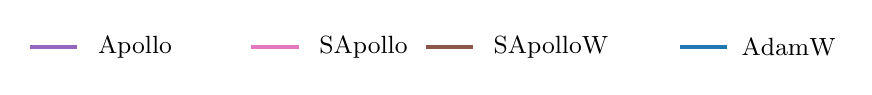
\begin{tikzpicture}[scale=0.75] % Nested TikZ environment
            \small 
            % AdaBelief
     \draw[mediumpurple148103189,  ultra thick] (0,0) -- ++(0.8,0);
     \node[anchor=west] at (1,0) {{Apollo}}; % Increased spacing
     
     % Adam
    
     \draw[orchid227119194,  ultra thick] (3.75,0) -- ++(0.8,0);
     \node[anchor=west] at (4.75,0) {{SApollo}}; % Increased spacing
     
     \draw[sienna1408675,  ultra thick] (6.7,0) -- ++(0.8,0);
     \node[anchor=west] at (7.7,0) {{SApolloW}}; % Increased spacing
     
     % Apollo
     \draw[steelblue31119180,  ultra thick] (11,0) -- ++(0.8,0);
     \node[anchor=west] at (11.9,0) {{AdamW}}; % Increased spacing
        
    \end{tikzpicture}
    };
    \end{tikzpicture}
     % Pfad zu deiner .tex-Datei
                \end{tabular}
                \caption{
                    Evaluation of \emph{SApollo} on CIFAR-10 using ResNet-110 with the \emph{cosine annealing} learning rate scheduler.
                }
                \label{fig:sapollo-perf}
            \end{minipage}
        \end{figure}
        